\documentclass[11 pt]{book}

\usepackage{amsthm,amsfonts,amssymb,amsmath}
\usepackage{delarray}
%\usepackage[paperheight=11in,paperwidth=8.5in,margin=0.75in]{geometry}
\usepackage{enumerate}
\usepackage[inline,shortlabels]{enumitem}
\usepackage{times}
\usepackage{comment}
\usepackage{graphics}
\usepackage{multicol}
\usepackage{appendix}
\usepackage{wrapfig}
%\usepackage{makeidx}
\usepackage{fancyhdr}
\usepackage{tikz}
\usepackage{pstricks}
\usepackage{afterpage}
\usepackage{verbatim}
\usepackage{rotating}
\usepackage[hyphens]{url}
\usepackage{hyperref}
%\usepackage[hyphens]{url}
\usepackage{lscape}
\usepackage{tabularx}
\usepackage{ctable}
\usepackage{color, colortbl}
\usepackage{caption}
\usepackage{epstopdf}
\definecolor{Blue}{rgb}{0,0,1}
\definecolor{Red}{rgb}{1,0,0}
\definecolor{Green}{rgb}{0,1,0}
\definecolor{Gray}{gray}{0.9}
\usepackage{imakeidx}
\makeindex

\addtolength{\oddsidemargin}{-.5in}
	\addtolength{\evensidemargin}{-.5in}
	\addtolength{\textwidth}{1.0in}

	\addtolength{\topmargin}{-.6in}
	\addtolength{\textheight}{1.3in}

\usepackage{hyperref}
\hypersetup{colorlinks=true, linkcolor=blue,  anchorcolor=blue,
citecolor=blue, filecolor=blue, menucolor=blue, pagecolor=blue,
urlcolor=blue,pdftitle={LA_main}}

%Path to images
\usepackage{graphicx}
\graphicspath{ {LA_Figures/} }
\DeclareGraphicsExtensions{.eps,.pdf,.png}

\makeatletter
\def\hlinewd#1{%
\noalign{\ifnum0=`}\fi\hrule \@height #1 %
\futurelet\reserved@a\@xhline}
\makeatother

\lhead[\fancyplain{}{\thepage}]         {\fancyplain{}{\rightmark}}
\chead[\fancyplain{}{}]                 {\fancyplain{}{}}
\rhead[\fancyplain{}{\rightmark}]      
 {\fancyplain{\tiny}}
%\resizebox{!}{0.15in}{\includegraphics{CClicense.eps}}}{\thepage}}
%\rfoot[\fancyplain{}{}] {\fancyplain{}{\tiny \resizebox{!}{0.20in}{\includegraphics{CClicense.eps}}}} \cfoot[\fancyplain{\thepage}{}]
%{\fancyplain{\thepage}{}} \lfoot[ \fancyplain{\resizebox{!}{0.20in}{\includegraphics{CClicense.eps}}} { \tiny \resizebox{!}{0.20in}{\includegraphics{CClicense.eps}}}] 
%{\fancyplain{}{}}

\let\origdoublepage\cleardoublepage
\newcommand{\clearemptydoublepage}{%
  \clearpage
  {\pagestyle{empty}\origdoublepage}%
}
\let\cleardoublepage\clearemptydoublepage

\DeclareMathOperator{\ch}{char}

\begin{document}
\renewcommand{\chaptername}{Section}
\newcommand{\achapter}[2]{\chapter{#2}\markboth{Section #1. #2}{Section #1. #2}}

%% Some theorem-like environments
\newtheorem{theorem}{Theorem}[chapter]
\newtheorem*{thm}{Theorem}
\newtheorem{lemma}[theorem]{Lemma}
\newtheorem{prop}[theorem]{Proposition}
\newtheorem{cor}[theorem]{Corollary}
\newtheorem{cnj}[theorem]{Conjecture}
\newtheorem{axiom}[theorem]{Axiom}
\newtheorem*{wop}{The Well-Ordering Principle}
\newtheorem*{divalg}{The Division Algorithm}
\newtheorem*{fta}{The Fundamental Theorem of Arithmetic}
\newtheorem*{el}{Euclid's Lemma}
\newtheorem*{thmstar}{Theorem}
\newtheorem*{lemstar}{Lemma}
\newtheorem*{claim}{Claim}
\theoremstyle{definition}
\newtheorem*{note}{Note}
\newtheorem{definition}[theorem]{Definition}
\newtheorem{idefn}[theorem]{Informal Definition}
\newtheorem{notation}[theorem]{Notation}
\newtheorem{ex}[theorem]{Example}
\newtheorem{example}[theorem]{Example}
\newtheorem{activity}{Activity}[chapter]
\newtheorem{pactivity}{Project Activity}[chapter]
\newtheorem{pa}{Preview Activity}[chapter]
\newtheorem{reflect}{Reflection}

\newtheoremstyle{activ} %
{9pt} % Space above
{3pt} % Space below
{} % Body font
{} % Indent amount
{\bfseries} % Theorem head font
{.} % Punctuation after theorem head
{ } % Space after theorem head
{} % Theorem head spec
%\newtheorem{question}{Activity}
%\newtheorem{question}{Activity}
\newtheorem{exercise}{Activity}[chapter]
\newtheorem{practice}{Exercise}[chapter]

\newsavebox{\smlmat}% Box to store smallmatrix content
\savebox{\smlmat}{$\left[\begin{smallmatrix}4\\6\end{smallmatrix}\right]$}

%% Common Number Sets
\newcommand{\Z}{\ensuremath{\mathbb{Z}}}
\newcommand{\E}{\ensuremath{\mathbb{E}}}
\newcommand{\N}{\ensuremath{\mathbb{N}}}
\newcommand{\W}{\ensuremath{\mathbb{W}}}
\newcommand{\Q}{\ensuremath{\mathbb{Q}}}
\newcommand{\R}{\ensuremath{\mathbb{R}}}
\newcommand{\C}{\ensuremath{\mathbb{C}}}
\newcommand{\J}{\ensuremath{\mathbb{J}}}
\newcommand{\F}{\ensuremath{\mathcal{F}}}
\newcommand{\D}{\ensuremath{\mathbb{D}}}
\newcommand{\M}{\ensuremath{\mathcal{M}}}
\newcommand{\B}{\ensuremath{\mathcal{B}}}
\newcommand{\NE}{\ensuremath{\mathcal{E}}}
\newcommand{\Mn}[1]{\ensuremath{\mathcal{M}_{#1 \times #1}}}
\renewcommand{\P}{\ensuremath{\mathcal{P}}}
\newcommand{\Rn}{\ensuremath{\R^n}}
\newcommand{\Mat}{\mathbf}
\newcommand{\Seq}{\boldsymbol}
\newcommand{\seq}[1]{\ensuremath{\boldsymbol{#1}}}
\newcommand{\set}[1]{\ensuremath{\mathcal{#1}}}
\newcommand{\abs}[1]{\left\lvert{}#1\right\rvert}
\newcommand{\floor}[1]{\ensuremath{\left\lfloor#1\right\rfloor}}
\newcommand{\cq}{\scalebox{.34}{\pscirclebox{\Huge \textbf{?}}}\hspace*{3 pt}}
\newcommand{\cqup}{\,$^{\text{\scalebox{.2}{\pscirclebox{\Huge\textbf{?}}}}}$}
\newcommand{\cqupmath}{\,^{\text{\scalebox{.2}{\pscirclebox{\Huge\textbf{?}}}}}}
\newcommand{\cqupmathnospace}{^{\text{\scalebox{.2}{\pscirclebox{\Huge\textbf{?}}}}}}
\newcommand{\uspace}[1]{\underline{\hphantom{~~#1~~~}}}
\newcommand{\muspace}[1]{\underline{\mspace{#1 mu}}}
\newcommand{\bspace}[1]{\hphantom{~~#1~~~}}
\newcommand{\ie}{\emph{i}.\emph{e}.}
\newcommand{\nq}[1]{\scalebox{.34}{\pscirclebox{\Huge\textbf{#1}}}}
\newcommand{\equalwhy}{\stackrel{\cqupmath}{=}}
\newcommand{\notequalwhy}{\stackrel{\cqupmath}{\neq}}
\newcommand{\Ker}{\text{Ker}}
\newcommand{\Image}{\text{Im}}
\renewcommand{\qedsymbol}{\ensuremath{\blacksquare}}
\newcommand{\polyp}{p(x) = a_nx^n + a_{n-1}x^{n-1} + \cdots a_2x^2 + a_1x + a_0}
\newcommand{\GL}{\text{GL}}
\newcommand{\SL}{\text{SL}}
\newcommand{\lcm}{\text{lcm}}
\newcommand{\Aut}{\text{Aut}}
\newcommand{\Inn}{\text{Inn}}
\newcommand{\Hol}{\text{Hol}}
\newcommand{\cl}{\text{cl}}
\newcommand{\bsq}{\hfill $\blacksquare$}
\newcommand{\NIMdot}{{\LARGE $\cdot$ }}
\newcommand{\eG}{\ensuremath{e_{\scriptscriptstyle{G}}}}
\newcommand{\eGroup}[1]{\ensuremath{e_{\scriptscriptstyle{#1}}}}
\newcommand{\Gdot}[1]{\ensuremath{\cdot_{\scriptscriptstyle{#1}}}}
\newcommand{\rbar}{\overline{r}}
\newcommand{\nuG}[1]{\ensuremath{\nu_{\scriptscriptstyle{#1}}}}
\newcommand{\rightarray}[2]{\left[ \begin{array}{#1} #2 \end{array} \right]}
\newcommand{\polymod}[1]{\mspace{5 mu}(\text{mod} #1)}
\newcommand{\ts}{\mspace{2 mu}}
\newcommand{\ds}{\displaystyle}
\newcommand{\adj}{\text{adj}}
\newcommand{\pol}{\mathbb{P}}
\newcommand{\CS}{\mathcal{S}}
\newcommand{\CC}{\mathcal{C}}
\newcommand{\CB}{\mathcal{B}}
\newcommand{\CD}{\mathcal{D}}
\newcommand{\CP}{\mathcal{P}}
\newcommand{\CQ}{\mathcal{Q}}
\newcommand{\CW}{\mathcal{W}}
\newcommand{\rank}{\text{rank}}
\newcommand{\nullity}{\text{nullity}}
\newcommand{\trace}{\text{trace}}
\newcommand{\Area}{\text{Area}}
\newcommand{\Vol}{\text{Vol}}
\newcommand{\cov}{\text{cov}}
\newcommand{\var}{\text{var}}

%vector commands
\newcommand{\va}{\mathbf{a}}
\newcommand{\vb}{\mathbf{b}}
\newcommand{\vc}{\mathbf{c}}
\newcommand{\vd}{\mathbf{d}}
\newcommand{\ve}{\mathbf{e}}
\newcommand{\vf}{\mathbf{f}}
\newcommand{\vg}{\mathbf{g}}
\newcommand{\vh}{\mathbf{h}}
\newcommand{\vm}{\mathbf{m}}
\newcommand{\vn}{\mathbf{n}}
\newcommand{\vp}{\mathbf{p}}
\newcommand{\vq}{\mathbf{q}}
\newcommand{\vr}{\mathbf{r}}
\newcommand{\vs}{\mathbf{s}}
\newcommand{\vx}{\mathbf{x}}
\newcommand{\vy}{\mathbf{y}}
\newcommand{\vu}{\mathbf{u}}
\newcommand{\vv}{\mathbf{v}}
\newcommand{\vw}{\mathbf{w}}
\newcommand{\vz}{\mathbf{z}}
\newcommand{\vzero}{\mathbf{0}}
\newcommand{\vi}{\mathbf{i}}
\newcommand{\vj}{\mathbf{j}}
\newcommand{\vk}{\mathbf{k}}
\newcommand{\vF}{\mathbf{F}}
\newcommand{\vP}{\mathbf{P}}

%Other commands
\newcommand{\nin}{\noindent}
\newcommand{\Dom}{\text{Dom}}
\newcommand{\tr}{\mathsf{T}}
\newcommand{\proj}{\text{proj}}
\newcommand{\comp}{\text{comp}}
\newcommand{\Row}{\text{Row }}
\newcommand{\Col}{\text{Col }}
\newcommand{\Nul}{\text{Nul }}
\newcommand{\Span}{\text{Span}}
\newcommand{\Range}{\text{Range}}
\newcommand{\Domain}{\text{Domain}}

\newcommand{\ExampleIntro}{\noindent What follows are worked examples that use the concepts from this section.}
\newcommand{\ExampleSolution}{\noindent \textbf{Example Solution. }}

\newcommand{\gr}{\varphi}
\newcommand{\grc}{\overline{\varphi}}


\newcommand{\hthin}{\hlinewd{.1pt}}
\newcommand{\hthick}{\hlinewd{.7pt}}
\newcommand{\vthick}{\vrule width .7pt}
\newcommand{\vthin}{\vrule width .1pt}

\newcommand{\pbreaks}{1} % Set to 1 to include pagebreaks, 0 otherwise

\newcommand{\pbreak}[0]%
{%
\ifthenelse{\equal{\pbreaks}{0}}{\medskip}{}%
\ifthenelse{\equal{\pbreaks}{1}}{\pagebreak}{}%
}


\makeatletter
\def\imod#1{\allowbreak\mkern8mu({\operator@font mod}\,\,#1)}
\makeatother


\long\def\symbolfootnote[#1]#2{\begingroup%
\def\thefootnote{\fnsymbol{footnote}}\footnote[#1]{#2}\endgroup}

\newcounter{cnt}
\newenvironment{numlist}{\begin{list}{(\arabic{cnt})}{\usecounter{cnt}
\setlength{\leftmargin}{.35 in}\setlength{\labelwidth}{.35 in}
\setlength{\itemsep}{10 pt}}}{\end{list}}

\newcounter{cnt4}
\newenvironment{numlist2}{\begin{list}{(\arabic{cnt4})}{\usecounter{cnt4}
\setlength{\leftmargin}{.5 in}\setlength{\labelwidth}{.25 in}
\setlength{\itemsep}{10 pt}}}{\end{list}}

\newcounter{cnt2}
\newenvironment{alphalist}{\vspace*{-3 pt}\begin{list}{(\alph{cnt2})}{\usecounter{cnt2}
\setlength{\leftmargin}{.5 in}\setlength{\labelwidth}{.25
in}\setlength{\itemsep}{5 pt}}}{\end{list}}

\newcounter{cnt3}
\newenvironment{alphalist2}{\vspace*{-3 pt}\begin{list}{(\alph{cnt3})}{\usecounter{cnt3}
\setlength{\leftmargin}{.25 in}\setlength{\labelwidth}{.25
in}\setlength{\itemsep}{5 pt}}}{\end{list}}

\newcounter{cnt5}
\newenvironment{thmlist}{\vspace*{-3 pt}\begin{list}{{(\roman{cnt5})}}{\usecounter{cnt5}
\setlength{\leftmargin}{.5 in}\setlength{\labelwidth}{.25
in}\setlength{\itemsep}{5 pt}}}{\end{list}}

\newcommand{\lint}{\raisebox{-.14 in}{\underline{\hspace*{.7 ex}}}
\hspace*{-1 ex} \int}

\newcommand{\uint}{\hspace*{1.5 ex} \raisebox{.296 in}{\underline{\hspace*{.7 ex}}}
\hspace*{-2.3 ex} \int}

\setlength{\parskip}{5 pt}

\newcounter{lastenum}
\newcommand{\saveCount}{\setcounter{lastenum}{\value{enumi}}}
\newcommand{\restoreCount}{\setcounter{enumi}{\value{lastenum}}}

\newcommand{\be}{\begin{numlist}}
\newcommand{\ee}{\end{numlist}}
\newcommand{\bei}{\begin{numlist2}}
\newcommand{\eei}{\end{numlist2}}
\newcommand{\ba}{\begin{alphalist}}
\newcommand{\ea}{\end{alphalist}}
\newcommand{\bal}{\begin{alphalist2}}
\newcommand{\eal}{\end{alphalist2}}
\newcommand{\bi}{\begin{itemize}}
\newcommand{\ei}{\end{itemize}}
\newcommand{\btl}{\begin{thmlist}}
\newcommand{\etl}{\end{thmlist}}
\newcommand{\solution}{\noindent \textbf{Solution. }}




%Ted's xitem


\renewcommand{\be}{\begin{enumerate}}
\renewcommand{\ee}{\end{enumerate}}
%\renewcommand{\ba}{\begin{enumerate}}
%\renewcommand{\ea}{\begin{enumerate}}

\renewcommand{\labelenumi}{(\arabic{enumi})}
%\renewcommand{\labelenumii}{(\arabic{enumii})}

\newcommand{\ans}{\renewcommand{\labelenumi}{$^\star$ (\arabic{enumi})}}
\newcommand{\ansend}{\renewcommand{\labelenumi}{(\arabic{enumi})}}
\newcommand{\xitem}{\ans \item \ansend}

%\newcommand{\xans}{\renewcommand{\labelenumii}{$^\star$ (\alph{enumii})}}
%\newcommand{\xansend}{\renewcommand{\labelenumii}{(\alph{enumii})}}
%\newcommand{\yitem}{\xans \item  \xansend}

\newlist{oddenumerate}{enumerate}{1} %odd number enumerate, need package \usepackage{enumitem}
\setlist[oddenumerate]{start=0,label=\theoddenumeratei.}
\makeatletter
\renewcommand\theoddenumeratei{\@arabic{\numexpr2*\value{oddenumeratei}+1}}
\makeatother

\newcommand{\obe}{\begin{oddenumerate}} 
\newcommand{\oee}{\end{oddenumerate}}

\makeatletter
\newcommand{\skipitems}[1]{%
  \addtocounter{\@enumctr}{#1}%
}
\makeatother

\renewcommand{\phi}{\varphi}
 
\newenvironment{fqs}{ \vspace*{7 pt}{\large \textbf{Focus Questions}} \vspace*{-6 pt} \\ ~\hrule~ \vspace*{2 pt}

 {\em By the end of this section, you should be able to give precise and thorough answers to the questions listed below.  You may want to keep these questions in mind to focus your thoughts as you complete the section.}
\vspace*{-5 pt} \\ ~\hrule~ \vspace*{-3 pt}
\begin{list}{\labelitemi}{\leftmargin=1.25em}
\setlength{\itemsep}{3 pt}}{ \end{list} \vspace*{-2 pt}}

\long\def\symbolfootnote[#1]#2{\begingroup%
\def\thefootnote{\fnsymbol{footnote}}\footnote[#1]{#2}\endgroup}

\newcommand{\csection}[1]{\section*{#1}\addcontentsline{toc}{section}{#1}}
\newcommand{\csubsection}[1]{\subsection*{#1}\addcontentsline{toc}{subsection}{#1}}

\renewcommand{\textfraction}{0.05}
\renewcommand{\topfraction}{0.95}
\renewcommand{\bottomfraction}{0.95}
\renewcommand{\floatpagefraction}{0.35}
\setcounter{totalnumber}{5}
\setcounter{topnumber}{5}
\setcounter{bottomnumber}{5}

\pagestyle{fancyplain}

\frontmatter{
\title{{\Huge An Inquiry-Based Introduction to Linear Algebra and Applications}  } }
\date{}

\author{\LARGE Feryal Alayont \\ ~\vspace*{-10 pt}~ \\ \LARGE Steven Schlicker \\ ~ \\ \LARGE Grand Valley State
University \\ \vspace*{.5 in} \\ \resizebox{!}{0.5in}{\includegraphics{CClicense.eps}}}

\maketitle

\thispagestyle{empty}

\renewcommand{\MakeUppercase}[1]{#1}

\tableofcontents

\input{0_preface.tex}

\mainmatter


%\begin{comment}

\part{Systems of Linear Equations}

\achapter{1}{Introduction to Systems of Linear Equations}\label{sec:intro_linear_systems}


\vspace*{-17 pt}
\framebox{
\parbox{\dimexpr\linewidth-3\fboxsep-3\fboxrule}
{\begin{fqs}
\item What is a linear equation?
\item What is a system of linear equations?
\item What is a solution set of a system of linear equations?
\item What are equivalent systems of linear equations?
\item What operations can we use to solve a system of linear equations?
\end{fqs}}}%\hspace*{3 pt}}

\vspace*{13 pt}

\csection{Application: Electrical Circuits}

Linear algebra is concerned with the study of systems of linear equations. There are two important aspects to linear systems. One is to use given information to set up a system of equations that represents the information (this is called \emph{modeling}), and the other is to solve the system.  As an example of modeling, we consider the application to the very simple electrical circuit. An electrical circuit consists of
\begin{itemize}
\item one or more electrical sources, denoted by \ \ \  \resizebox{!}{0.25in}{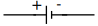
\includegraphics{1_a_pa_source}}
\item one or more resistors, denoted by \ \ \ 
\resizebox{!}{0.25in}{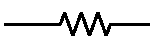
\includegraphics{1_a_pa_resistor}}.
\end{itemize}
A source\index{circuits!source} is a power supply like a battery, and a resistor\index{circuits!resistor} is an object that consumes the electricity, like a lamp or a computer. A simple circuit consists of one or more sources connected to resistors, like the one shown in Figure \ref{F:circuit1}. The straight lines in the circuit indicate wires through which current flows. The points labeled P and Q are called \emph{junctions} or \emph{nodes}\index{circuits!junctions}.
\begin{figure}[h]
\begin{center}
\resizebox{!}{2.5in}{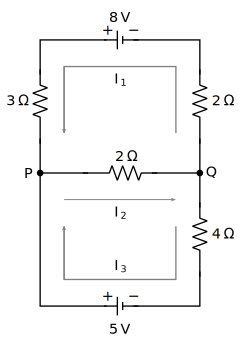
\includegraphics{1_a_pa_circuit1.eps}}
\end{center}
\caption{A circuit.}
\label{F:circuit1}
\end{figure}

The source creates a charge that produces potential energy $E$ measured in volts (V).  Current flows out of the positive terminal of a source and runs through each branch of the circuit. Let $I_1$, $I_2$, and $I_3$ be the currents as illustrated in  Figure \ref{F:circuit1}. The goal is to find the current flowing in each branch of the circuit.  

Linear algebra comes into play when analyzing a circuit based on the relationship between current $I$, resistance $R$, and voltage $E$. There are laws governing electrical circuits that state that $E = IR$ across a resistor. Additionally, Kirchoff's Current and Voltage Laws indicate how current behaves within the whole circuit. Using all these laws together, we derive the system
\begin{alignat}{4}
{}I_1 \	&- \	&{}I_2 \	&+ \	&{}I_3 \	&= 0  \notag \\ %\label{eq:circuit_1} \\
5I_1 \	&+ \	&2I_2 \		&{} \ 	&{}  \		&= 8 \notag \\ %\label{eq:circuit_2} \\
	\	&{} \ 	&2I_2 \		&+ \	&4I_3 \		&= 5, \notag %\label{eq:circuit_3}
\end{alignat}
where $I_1$, $I_2$, and $I_3$ are the currents at the points indicated in Figure \ref{F:circuit1}. To finish analyzing the circuit, we now need to solve this system. In this section we will begin to learn systematic methods for solving systems of linear equations. More details about the derivation of these circuit equations can be found at the end of this section.  

\csection{Introduction}

Systems of linear equations  arise in almost every field of study: mathematics, statistics, physics, chemistry, biology, economics, sociology, computer science, engineering, and many, many others. We will study the theory behind solving systems of linear equations, implications of this theory, and applications of linear algebra as we proceed throughout this text. 

\begin{pa} \label{pa:1_a} ~
\be
\item \label{ex:system_1} Consider the following system of two linear equations in two unknowns, $x_1, x_2$: 
\begin{alignat}{4}
2x_1	&{}-{}	&3x_2 	&= 0  \notag \\%\label{eq:PA1.1_1} \\
x_1 	&{}-{} 	&x_2		&= 1. \notag %\label{eq:PA1.1__2} 
\end{alignat}


One way to solve such a system of linear equations is the method of substitution (where one equation is solved for one variable and then the resulting expression is substituted into the remaining equations). This method works well for simple systems of two equations in two unknowns, but becomes complicated if the number or complexity of the equations is increased. 

Another method is elimination -- the method that we will adopt in this book. Recall that the elimination method works by multiplying each equation by a suitable constant so that the coefficients of one of the variables in each equation is the same. Then we subtract corresponding sides of these equations to eliminate that variable. 

Use the method of elimination to show that this system has the unique solution $x_1=3$ and $x_2=2$. Explain the specific steps you perform when using elimination. 

\item Recall that a linear equation in two variables can be represented as a line in $\R^2$, the Cartesian plane, where one variable corresponds to the horizontal axis and the other to the vertical axis. Represent the two equations $2x_1 -3x_2 = 0$ and $x_1 - x_2= 1$ in $\R^2$ and illustrate the solution to the system in your picture.

\item The previous example should be familiar to you as a system of two equations in two unknowns. Now we consider a system of three equations in three unknowns 
\begin{alignat}{4}
{}I_1 	&{}-{} 	&{}I_2	&{}+{}	&{}I_3 	&{}={} 	&0&{}  \label{eq:PAcircuit_a} \\
{5}I_1 	&{}+{}	&{2}I_2 	&{} 		&{} 		&{}={}	&8&{} \label{eq:PAcircuit_b} \\
{}		&{} 	 	&{2}I_2 	&{}+{}	& {4}I_3	&{}={}	&5&{} \label{eq:PAcircuit_c}
\end{alignat}
that arises from our electrical circuit in Figure \ref{F:circuit1}, with currents $I_1$, $I_2$, and $I_3$ as indicated in the circuit. 
\begin{figure}[h]
\begin{center}
\resizebox{!}{2.5in}{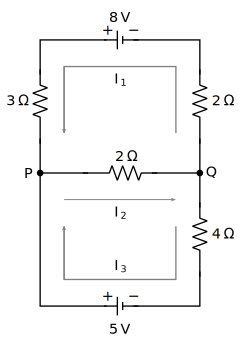
\includegraphics{1_a_pa_circuit1.eps}}
\end{center}
\caption{A circuit.}
\label{F:circuit1}
\end{figure}
In the remainder of this preview activity we will apply the method of elimination to solve the system of linear equations (\ref{eq:PAcircuit_a}), (\ref{eq:PAcircuit_b}), and (\ref{eq:PAcircuit_c}). 

    \ba
            \item Replace equation (\ref{eq:PAcircuit_b}) with the new equation obtained by multiplying both sides of equation (\ref{eq:PAcircuit_a}) by 5 and then subtracting corresponding sides of this equation from the appropriate sides of equation (\ref{eq:PAcircuit_b}).  Show that the resulting system is
        \begin{alignat}{4}
{}I_1 \	&- \	&{}I_2 \	&+ \	&{}I_3 \	&= 0  \notag \\
     \	&  \	&7I_2  \		&{-} \ 	&{5}I_3  \		&= 8 \label{eq:PAcircuit_d} \\
	\	&{} \ 	&2I_2 \		&+ \	&4I_3 \		&= 5. \notag
    \end{alignat}


         \item Now eliminate the variable $I_2$ from the last two equations in the system in part (a) by using equations (\ref{eq:PAcircuit_c}) and (\ref{eq:PAcircuit_d}) to show that $I_3=0.5$. Explain your process. 

        \item Once you know the value for $I_3$, how can you find $I_2$? Then how do you find $I_1$? Use your method to show that the solution to this system is the ordered triple (1,1.5,0.5). Interpret the result in terms of currents. 

	\ea

\ee

\end{pa}

\csection{Notation and Terminology}

To study linear algebra, we will need to agree on some general notation and terminology to represent our systems. 

An equation like $4x_1 + x_2 = 8$ is called a linear equation because the variables ($x_1$ and $x_2$ in this case) are raised to the first power, and there are no products of variables. The equation $4x_1 + x_2 = 8$ is a linear equation in two variables, but we can make a linear equation with any number of variables we like. 

\begin{definition} A \textbf{linear equation}\index{linear equation} in the variables $x_1$, $x_2$, $\ldots$, $x_n$ is an equation of the form
\[a_1x_1 + a_2x_2 + \cdots + a_nx_n = b,\]
where $n$ is a positive integer and $a_1$, $a_2$, $\ldots$, $a_n$ and $b$ are constants. The constants $a_1$, $a_2$, $\ldots$, $a_n$ are called the \textbf{coefficients}\index{linear equation!coefficients} of the equation. 
\end{definition}

We can use any labels for the variables in a linear equation that we like, e.g., $I_1$, $x_1$, $t_1$, and you should become comfortable working with variables in any form. We will usually use subscripts, as in $x_1, x_2, x_3, \ldots$, to represent the variables as this notation allows us to have any number of variables. Other examples of linear equations are 
\[ x+2y=4 \quad \text{ and } \quad \sqrt{2}x_1-3x_2=\frac{1}{4}x_3+\pi \, .\]
On the other hand, the equations
\[\frac{1}{x}+y-z=0 \quad \text{ and } \quad 2x_1=\sqrt{x_2}-5 \]
are non-linear equations. 

\begin{definition} A \textbf{system of linear equations}\index{system of linear equations} is a collection of one or more linear equations in the same variables. 
\end{definition}

For example, the two equations 

\begin{equation} \label{eq:1_a_PA_1}
\begin{alignedat}{4}
x_1 	&{}-{}	&x_2	&= 1  \\ 
2x_1 	&{}+{} 	&x_2	&= 5 
\end{alignedat}
\end{equation}
form a system of two linear equations in variables $x_1$, $x_2$.

\begin{definition} A \textbf{solution}\index{system of linear equations!solution} to a system of linear equations is an ordered $n$-tuple $(s_1, s_2, \ldots, s_n)$ of numbers so that we obtain all true statements in the system when we replace the variable in order with $s_1$, $s_2$, $\ldots$, and  $s_n$. 
\end{definition}

For example, $x_1=2, x_2=1$, or simply $(2,1)$, is a solution to the above system of linear equations in \eqref{eq:1_a_PA_1} as can be checked by substituting the variables into each equation. In solving a system of linear equations, we are interested in finding the set of all solutions, which we will call the \emph{solution set of the system}\index{system of linear equations!solution set}. For the above system in \eqref{eq:1_a_PA_1}, the solution set is the set containing the single point $(2,1)$, denoted $\{(2,1)\}$, because there is only one solution. If we consider just the equation $x_1-x_2=0$ as our system, the solution set is the line $x_1=x_2$ in the plane. More generally, a set of solutions is a collection of ordered $n$-tuples of numbers. We denote the set of all ordered $n$-tuples of numbers as $\R^n$. So, for example, $\R^2$ is the set of all ordered pairs, or just the standard coordinate plane, and $\R^3$ is the set of all ordered triples, or the three-dimensional space. 


\csection{Solving Systems of Linear Equations}

In Preview Activity \ref{pa:1_a}, we were introduced to linear systems and the method of elimination for a system of two or three variables. Our goal now is to come up with a systematic method that will reduce any linear system to one that is easy to solve without changing the solution set of the system. Two linear systems will be called \emph{equivalent}\index{system of linear equations!equivalent systems} if they have the same solution set. 

The operations we used in Preview Activity \ref{pa:1_a} to systematically eliminate variables so that we can solve a linear system are called \emph{elementary operations on a system of linear equations} or just \emph{elementary operations}\index{elementary operations}\index{system of linear equations!operations}. In the exercises you will argue that elementary operations do not change the solution set to a system of linear equations, a fact that is summarized in the following theorem.

\begin{theorem} The \textbf{elementary operations} on a system of linear equations: 
\begin{enumerate}
\item replacing one equation by the sum of that equation and a scalar multiple of another equation;
\item interchanging two equations;
\item replacing an equation by a nonzero scalar multiple of itself;
\end{enumerate}
do not change the solution set to the system of equations.
\end{theorem}

When we apply these elementary operations our ultimate goal is to produce a system of linear equations in a simplified form with the same solution set, where the number of variables eliminated from the equations increase as we move from top to bottom. This method is called the \emph{elimination}\index{system of linear equations!elimination} method. 

\begin{activity} For systems of linear equations with a small number of variables, many different methods could be used to find a solution. However, when a system gets large, ad-hoc methods become unwieldy. One of our goals is to develop an algorithmic approach to solving systems of linear equations that can be programmed and applied to any linear system, so we want to work in a very prescribed method as indicated in this activity. Ultimately, once we understand how the algorithm works, we will use calculators/computers to do the work. Apply the elimination method as described to show that the solution set of the following system is $(2, -1, 1)$:
\begin{alignat*}{4}
x_1 &{}+{}& x_2 &{}-{}& x_3 &= 0   \\
2x_1 &{}+{}& x_2 &{}-{}& x_3 &= 2  \\
x_1&{}-{}&x_2 &{}+{}& 2x_3 &= 5. 
\end{alignat*}
	\ba
	\item Use the first equation to eliminate the variable $x_1$ in the second and third equations.
	
	\item Use the new second equation to eliminate the variable $x_2$ in the third equation and find the value of $x_3$. 
	
	\item Find values of $x_2$ and then $x_1$.

	
	\ea
	
\end{activity}



\noindent \textbf{Important Note:} Technically, we don't really add two equations or multiply an equation by a scalar. When we refer to a scalar multiple of an equation, we mean the equation obtained by equating the scalar multiple of the expression on the left side of the equation and the same scalar multiple of the expression on the right side of the equation. Similarly, when we refer to a sum of two equations, we don't really add the equations themselves. Instead, we mean the equation obtained by equating the sum of the expressions on the left sides of the equations to the sum of the expressions on the right sides of the equations. We will use the terminology ``scalar multiple of an equation" and ``sum of two equations" as shorthand to mean what is described here.


\noindent \textbf{Another Important Note:} There is an important and subtle point to consider here. When we use these operations to find a solution to a system of equations, we are assuming that the system has a solution. The application of these operations then tells us what a solution must look like. However, there is no guarantee that the outcome is actually a solution -- to be safe we should check to make sure that our result is a solution to the system. In the case of linear systems, though, every one of our operations on equations is reversible (if applied correctly), so the result will always be a solution (but this is not true in general for non-linear systems).  


\noindent \textbf{Terminology:} A system of equations is called \emph{consistent}\index{system of linear equations!consistent} if the system has at least one solution. If a system has no solutions, then it is said to be \emph{inconsistent}\index{system of linear equations!inconsistent}.

\csection{The Geometry of Solution Sets of Linear Systems}

We are familiar with linear equations in two variables from basic algebra and calculus (through linear approximations). The set of solutions to a system of linear equations in two variables has some geometry connected to it.


\begin{activity} \label{act:1_a_2} Recall that we examined the geometry of the system 
\begin{alignat}{4}
2x_1 	&{}-{}	&3x_2 	&= 0  \notag \\%\label{eq:PA1.1_1} \\
x_1 	&{}-{} 	&x_2		&= 1 \notag %\label{eq:PA1.1__2} 
\end{alignat}
in Preview Activity \ref{pa:1_a} to show that the resulting solution set consists of a single point in the plane.

In this activity we examine the geometry of the system 
\begin{equation}\label{eq:1_a_2}
\begin{alignedat}{4}
{2}x_1 	&{}-{}	&{}x_2 	&= 1&{}  \\ %\notag \\%\label{eq:PA1.1_1} \\
{2}x_1 	&{}-{} 	&{2}x_2		&= 2&{.} % \notag %\label{eq:PA1.1__2} 
\end{alignedat}
\end{equation}
\ba
\item Consider the linear equation $2x_1-2x_2=2$ (or, equivalently $2x-2y=2$). What is the graph of the solution set (the set of points $(x_1, x_2)$ satisfying this equation) of this single equation in the plane? Draw the graph to illustrate. 


\item How can we represent the solution set of the system \eqref{eq:1_a_2} of two equations graphically? How is this solution set related to the solution set of the single equation $2x_1-2x_2=2$? Why? How many solutions does the system \eqref{eq:1_a_2} have? 


\item There are exactly three possibilities for the number of solutions to a general system of two linear equations in two unknowns. Describe the geometric representations of solution sets for each of the possibilities. Illustrate each with a specific example (of your own) using a system of equations and sketching its geometric representation. 

\ea

\end{activity}

Activity \ref{act:1_a_2} shows that there are three options for the solution set of a system: A system can have no solutions, one solution, or infinitely many solutions.


Now we consider systems of three variables. As an example, let us look at the linear equation $x+y+z=1$ in the three variables $x$, $y$, and $z$. Notice that the points $(1,1,-2)$, $(0,0,0)$, and $(-1,-1,2)$ all satisfy this equation. As a linear equation, the graph of $x+y+z=0$ will be a plane in three dimensions that contains these three points, as shown in Figure \ref{F:1_a_plane}. Hence when we consider a linear system in three unknowns, we are looking for a point in the three dimensional space that lies on all the planes described by the equations. 

\begin{figure}[h]
\begin{center}
\resizebox{!}{2.0in}{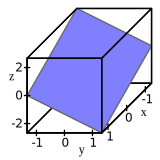
\includegraphics{1_a_plane.eps}}
\caption{The plane $x+y+z=1$.}
\label{F:1_a_plane}
\end{center}
\end{figure}

\begin{activity} \label{act:1_a_3} In this activity we examine the geometry of linear systems of three equations in three unknowns. Recall that each linear equation in three variables has a plane as its solution set. Use a piece of paper to represent each plane. 
\ba
\item Is it possible for a general system of three linear equations in three unknowns to have no solutions? If so, geometrically describe this situation and then illustrate each with a specific example using a system of equations. If not, explain why not.


\item Is it possible for a general system of three linear equations in three unknowns to have exactly one solution? If so, geometrically describe this situation and then illustrate each with a specific example using a system of equations. If not, explain why not.
 

\item Is it possible for a general system of three linear equations in three unknowns to have infinitely many solutions? If so, geometrically describe this situation and then illustrate each with a specific example using a system of equations. If not, explain why not.

 


\ea

\end{activity}


\csection{Examples}

\ExampleIntro

\begin{example} Apply the allowable operations on equations to solve the system
\begin{alignat*}{5}
{}x_1	 	&{}+{}	&{2}x_2 	&{+}	&{}x_3	&{-}	&{}x_4	&= 4&{}   \\
{}	 	&{}-{}	&{}x_2 	&{-}	&{}x_3	&{+}	&{3}x_4	&= 6&{}   \\
{}x_1 	&{}{}		&{}	 	&{+}	&{2}x_3	&{-}	&{}x_4	&= 1&{}   \\
{2}x_1	 &{}-{}	&{3}x_2 	&{+}	&{}x_3	&{+}	&{}x_4	&= 2&{.}   
\end{alignat*}

\ExampleSolution We begin by eliminating the variable $x_1$ from all but the first equation. To do so, we replace the third equation with the third equation minus the first equation to obtain the equivalent system
\begin{alignat*}{5}
{}x_1	 	&{}+{}	&{2}x_2 	&{+}		&{}x_3	&{-}	&{}x_4	&= {}&4&{}   \\
{}	 	&{}-{}	&{}x_2 	&{-}		&{}x_3	&{+}	&{3}x_4	&= {}&6&{}   \\
{}	 	&{}-{}	&{2}x_2	 &{+}		&{}x_3	&{}	&{}		&= {-}&3&{}   \\
{2}x_1	 &{}-{}	&{3}x_2 	&{+}		&{}x_3	&{+}	&{}x_4	&= {}&2&{.}   
\end{alignat*}
Then we replace the fourth equation with the fourth equation minus 2 times the first to obtain the equivalent system
\begin{alignat*}{5}
{}x_1	 	&{}+{}	&{2}x_2 	&{+}		&{}x_3	&{-}	&{}x_4	&= {}&4&{}   \\
{}	 	&{}-{}	&{}x_2 	&{-}		&{}x_3	&{+}	&{3}x_4	&= {}&6&{}   \\
{}	 	&{}-{}	&{2}x_2	 &{+}		&{}x_3	&{}	&{}		&= {-}&3&{}   \\
{}	 	&{}-{}	&{7}x_2 	&{-}		&{}x_3	&{+}	&{3}x_4	&= {-}&6&{.}   
\end{alignat*}

To continue the elimination process, we want to eliminate the $x_2$ variable from our latest third and fourth equations. To do so, we use the second equation so that we do not reinstate an $x_1$ variable in our new equations. We replace equation three with equation 3 minus 2 times equation 2 to produce the equivalent system
\begin{alignat*}{5}
{}x_1	 	&{}+{}	&{2}x_2 	&{+}		&{}x_3	&{-}	&{}x_4	&= {}&4&{}   \\
{}	 	&{}-{}	&{}x_2 	&{-}		&{}x_3	&{+}	&{3}x_4	&= {}&6&{}   \\
{}	 	&{}{}		&{}		&{ }		&{3}x_3	&{-}	&{6}x_4	&= {-}&15&{}   \\
{}	 	&{}-{}	&{7}x_2 	&{-}		&{}x_3	&{+}	&{3}x_4	&= {-}&6&{.}   
\end{alignat*}
Then we replace equation four with equation four minus 7 times equation 2, giving us the equivalent system
\begin{alignat*}{5}
{}x_1	 	&{}+{}	&{2}x_2 	&{+}		&{}x_3	&{-}	&{}x_4	&= {}&4&{}   \\
{}	 	&{}-{}	&{}x_2 	&{-}		&{}x_3	&{+}	&{3}x_4	&= {}&6&{}   \\
{}	 	&{}{}		&{}		&{ }		&{3}x_3	&{-}	&{6}x_4	&= {-}&15&{}   \\
{}	 	&{}{}		&{}	 	&{ }		&{6}x_3	&{-}	&{18}x_4	&= {-}&48&{.}   
\end{alignat*}

With one more step we can determine the value of $x_4$. We use the last two equations to eliminate $x_3$ from the fourth equation by replacing equation four with equation four minus 2 times equation 3. This results in the equivalent system
\begin{alignat*}{5}
{}x_1	 	&{}+{}	&{2}x_2 	&{+}		&{}x_3	&{-}	&{}x_4	&= {}&4&{}   \\
{}	 	&{}-{}	&{}x_2 	&{-}		&{}x_3	&{+}	&{3}x_4	&= {}&6&{}   \\
{}	 	&{}{}		&{}		&{ }		&{3}x_3	&{-}	&{6}x_4	&= {-}&15&{}   \\
{}	 	&{}{}		&{}	 	&{}		&{}		&{-}	&{6}x_4	&= {-}&18&{.}   
\end{alignat*}

The last equation tells us that $-6x_4 = -18$, or $x_4 =3$. Substituting into the third equation shows that 
\begin{align*}
3x_3 - 6\left(3\right) &= -15 \\
3x_3 &= 3 \\
x_3 &= 1.
\end{align*}
The second equation shows that
\begin{align*}
-x_2 - 1 + 3\left(3\right) &= 6 \\
-x_2 &= -2 \\
x_2 &=2.
\end{align*}
Finally, the first equation tells us that
\begin{align*}
x_1 + 2\left(2\right) + 1 - 3 &= 4 \\
x_1 &= 2. 
\end{align*}

So the solution to our system is $x_1 =2$, $x_2 = 2$, $x_3 = 1$, and $x_4 =3$. It is worth substituting back into our original system to check to make sure that we have not made any arithmetic mistakes. 
\end{example}

\begin{example} A mining company has three mines. One day of operation at the mines produces the following output.
\begin{itemize}
\item Mine 1 produces 25 tons of copper, 600 kilograms of silver and 15 tons of manganese.
\item Mine 2 produces 30 tons of copper, 500 kilograms of silver and 10 tons of manganese.
\item Mine 3 produces 20 tons of copper, 550 kilograms of silver and 12 tons of manganese.
\end{itemize}
Suppose the company has orders for 550 tons of copper, 11350 kilograms of silver and 250 tons of manganese.

Write a system of equations to answer the question: how many days should the company operate each mine to exactly fill the orders? State clearly what the variables in your system represent. Then find the general solution of your system. \\

	
\ExampleSolution For our system, let $x_1$ be the number of days mine 1 operates, $x_2$ be the number of days mine 2 operates, and $x_3$ be the number of days mine 3 operates. Since mine 1 produces 25 tons of copper each day, in $x_1$ days mine 1 will produce $25x_1$ tons of copper. Mine 2 produces 30 tons of copper each day, so in $x_2$ days mine 2 will produce $30x_2$ tons of copper. Also, mine 3 produces 20 tons of copper each day, so in $x_3$ days mine 3 will produce $20x_3$ tons of copper. Since the company needs to supply a total of 550 tons of copper, we need to have $25x_1+30x_2+20x_3 = 550$. Similar analyses of silver and manganese give us the system
\begin{alignat*}{4}
{25}x_1  	&{}+{}	&{30}x_2	&{}+{} 	&{20}x_3	&{}={} 	&550&{}  \\
{600}x_1  	&{}+{}  &{500}x_2	&{}+{}  &{550}x_3 	&{}={} 	&11350&{}  \\
{15}x_1    	&{}+{}	&{10}x_2  	&{}+{}  &{12}x_3   &{}={}	&250&{.}
 \end{alignat*}  
 
 To solve the system, we eliminate the variable $x_2$ from the second and third equations by replacing equation two with equation two minus 24 times equation one and replacing equation three with equation three minus $\frac{3}{5}$ times equation one. This produces the equvalent system 
\begin{alignat*}{5}
{25}x_1  	&{}+{}	&{30}x_2	&{}+{} 	&{20}x_3	&{}={} 	&{}550&{}  \\
{}  		&{}-{}  	&{220}x_2	&{}+{}  	&{70}x_3 	&{}={} 	&{-}1850&{}  \\
{}    		&{}-{}	&{8}x_2  	&{}{}  	&{}   		&{}={}	&{-}80&{.}
 \end{alignat*}  
We are fortunate now that we can determine the value of $x_2$ from the third equation, which tells us that $x_2 = 10$. Substituting into the second equation shows that 
\begin{align*}
-220(10) + 70x_3 &= -1850 \\
70x_3 &= 350 \\
x_3 &= 5.
\end{align*}
Substituting into the first equation allows us to determine the value for $x_1$:
 \begin{align*}
 25x_1 + 30(10) + 20(5) &= 550 \\
 25x_1 &= 150 \\
 x_1 &= 6.
 \end{align*}
So the company should run mine 1 for 6 days, mine 2 for 10 days, and mine 3 for 5 days to meet this demand.

\end{example}

\csection{Summary}
In this section we introduced linear equations and systems of linear equations. 
\begin{itemize}
\item Informally, a linear equation is an equation in which each term is either a constant or a constant times a variable. More formally, a linear equation in the variables $x_1$, $x_2$, $\ldots$, $x_n$ is an equation of the form
\[a_1x_1 + a_2x_2 + \cdots + a_nx_n = b,\]
where $n$ is a positive integer and $a_1$, $a_2$, $\ldots$, $a_n$ and $b$ are constants.
\item A system of linear equations is a collection of one or more linear equations in the same variables.
\item Informally, a solution to a system of linear equations is a point that satisfies all of the equations in the system. More formally, a solution to a system of linear equation in $n$ variables $x_1$, $x_2$, $\ldots$, $x_n$ is an ordered $n$-tuple $(s_1, s_2, \ldots, s_n)$ of numbers so that we obtain all true statements in the system when we replace $x_1$ with $s_1$, $x_2$ with $s_2$, $\ldots$, and $x_n$ with $s_n$.
\item Two linear systems are equivalent if they have the same solution set. 
\item The following operations on a system of equations do not change the solution set: 
\begin{enumerate}
\item Replace one equation by the sum of that equation and a scalar multiple of another equation.
\item Interchange two equations.
\item Replace an equation by a nonzero scalar multiple of itself.
\end{enumerate}
\end{itemize}




\csection{Exercises}
\be

\item In the method of elimination there are three operations we can apply to solve a system of linear equations. For this exercise we focus on a system of equations in three unknowns $x_1$, $x_2$, and $x_3$, but the arguments generalize to a system with any number of variables. Consider the general system of three equations in three unknowns
\begin{alignat*}{4}
4x_1 	&{}-{}	&4x_2	&{}+{}	&4x_3 	&= 0  \\ 
4x_1 	&{}+{}	&2x_2	&{}		&{} 		&= 8  \\
{} 	&{}		&2x_2	&{}+{}	&5x_3	&= 9.  
\end{alignat*}
The goal of this exercise is to understand why the three operations on a system do not change the solutions to the system. Recall that a solution to a system with unknowns $x_1$, $x_2$, and $x_3$ is a set of three numbers, one for $x_1$, one for $x_2$, and one for $x_3$ that satisfy all of the equations in the system. 
	\ba
	\item Explain why, if we have a solution to this system, then that solution is also a solution to any constant $k$ times the second equation.  

    \item Explain why, if we have a solution to this system, then that solution is also a solution to the sum of the first equation and $k$ times the third equation for any constant $k$. 

	\ea

\item Alice stopped by a coffee shop two days in a row at a conference to buy drinks and pastries. On the first day, she bought a cup of coffee and two muffins for which she paid \$6.87. The next day she bought two cups of coffee and three muffins (for herself and a friend). Her bill was \$11.25. Use the method of elimination to determine the price of a cup of coffee, and the price of a muffin. Clearly explain your set-up for the problem. (Assume you are explaining your solution to someone who has not solved the problem herself/himself).

\item Alice stopped by a coffee shop three days in a row at a conference to buy drinks and pastries. On the first day, she bought a cup of coffee, a muffin and a scone for which she paid \$6.15. The next day she bought two cups of coffee, three muffins and a scone (for herself and friends). Her bill was \$12.20. The last day she bought a cup of coffee, two muffins and two scones, and paid \$10.35. Determine the price of a cup of coffee, the price of a muffin and the price of a scone. Clearly explain your set-up for the problem. (Assume you are explaining your solution to someone who has not solved the problem herself/himself).

\item 
	\ba
	\item Find an example of a system of two linear equations in variables $x$, $y$ for each of the following three cases: 
		\begin{enumerate}[i.]
		\item where the equations correspond to two non-parallel lines, 
		\item two parallel distinct lines, 
		\item two identical lines (represented with different equations). 
		\end{enumerate}
	\item Describe how the relationship between the coefficients of the variables of the two equations in parts (ii) and (iii) are different than the relationship between those coefficients in part (i) (Note: Please make sure your system examples are different than the examples in the activities, and that they are your own examples.)
	\ea

\item In a grid of wires in thermal equilibrium, the temperature at interior nodes is the average of the temperatures at adjacent nodes. Consider the grid as shown in Figure \ref{F:Grid}, with $x_1$, $x_2$, and $x_3$ the temperatures (in degrees Centigrade) at the indicated interior nodes, and fixed temperatures at the other nodes as shown. For example, the nodes adjacent to the node with temperature $x_1$ have temperatures of $x_2$, $200$, $0$, and $0$, so when the grid is in thermal equilibrium $x_1$ is the average of these temperatures:
\[x_1 = \frac{x_2+200+0+0}{4}.\]
\begin{figure}[h]
\begin{center}
\resizebox{!}{1.5in}{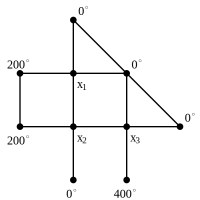
\includegraphics{Grid.eps}}
\caption{A grid of wires.}
\label{F:Grid}
\end{center}
\end{figure}
	\ba
	\item Determine equations for the temperatures $x_2$ and $x_3$ if the grid is in thermal equilibrium to construct a system of three linear equations in $x_1$, $x_2$, and $x_3$ that models node temperatures in the grid in thermal equilibrium.

	\item Use the method of elimination to find a specific solution to the system that makes sense in context.  

	\ea

\item We have seen that a linear system of two equations in two unknowns can have no solutions, one solution, or infinitely many solutions. Find, if possible, a specific example of each of the following. If not possible, explain why.
	\ba
	\item A linear system of three equations in two unknowns with no solutions.
	\item A linear system of three equations in two unknowns with exactly one solution.
	\item A linear system of three equations in two unknowns with exactly two solutions.
	\item A linear system of three equations in two unknowns with infinitely many solutions.
	\ea

\item We have seen that a linear system of three equations in three unknowns can have no solutions, one solution, or infinitely many solutions. Find, if possible, a specific example of each of the following. If not possible, explain why.
	\ba
	\item A linear system of two equations in three unknowns with no solutions.
	\item A linear system of two equations in three unknowns with exactly one solution.
	\item A linear system of two equations in three unknowns with exactly two solutions.
	\item A linear system of two equations in three unknowns with infinitely many solutions.
	\ea
		
\item Find a system of three linear equations in two variables $u$, $v$ whose solution is $u=2$, $v=1$.

\item Consider the system of linear equations
\begin{alignat*}{3}
x_1 	& {}+{} & hx_2 & {}={} & 2 \\
3x_1 	& {}+{} & 5x_2 & {}={} & 1 
\end{alignat*}
where $h$ is an unknown constant. 
	\ba
	\item  Determine the solution(s) of this system for all possible $h$ values, if a solution exists. (Note: Your answers for the variables will depend on the $h$.)
	\item How do your answers change if the second equation in the system above is changed to $3x_1+5x_2=6$?\\
	
	\ea
	
\item Suppose we are given a system of two linear equations
\begin{alignat}{4}
x_1 	& {}+{} & 2x_2 	& {}-{} 	& x_3{}={} 	& { } &1&{} \label{eq_1} \\
3x_1 	& {}+{} & x_2 	& {}+{} 	& 2x_3{}={} 	& {-} &1&. \label{eq_2} 
\end{alignat}
Find another system of two linear equations $E_1$ and $E_2$ in the variables $x_1$, $x_2$, and $x_3$ that are not multiples of each other or of equations (\ref{eq_1}) or (\ref{eq_2}) so that any solution $(x_1, x_2, x_3)$ to the system (\ref{eq_1}) and (\ref{eq_2}) is a solution to the system $E_1$ and $E_2$. 

\ee

\csection{True/False Questions}

In many sections you will be given True/False questions. In each of the True/False questions, you will be given a statement, such as ``if we add corresponding sides of two linear equations, then the resulting equation is a linear equation" and ``one can find a system of two equations in two unknowns that has infinitely many solutions." Your task will be to determine the truth value of the statement and to give a brief justification for your choice.



Note that a {\em general} statement is considered {\em true} only when it is always true. For example, the first of the above statements -- ``if we add corresponding sides of two linear equations, then the resulting equation is a linear equation" -- is a general statement. For this statement to be true, the equation we obtain by adding corresponding sides of any two linear equations has to be linear. If we can find two equations that do not give a linear equation when combined in this way, then this statement is false.



Note that an {\em existential} statement is considered {\em true} if there is at least one example which makes is true. For example, the latter of the above statements -- ``one can find a system of two equations in two unknowns that has infinitely many solutions" -- is an existential statement. For this statement to be true, existence of a system of two equations in two unknowns with infinitely many solutions should suffice. If it is impossible to find two such equations, then this statement is false.



To justify that something always happens or never happens, one would need to refer to other statements whose truth is known, such as theorems, definitions. In particular, giving an \textbf{example} of two linear equations that produce a linear equation when we add corresponding sides \emph{does not justify} why the sum of \textbf{any} two linear equations is also linear. Using the definition of linear equations, however, we can justify why this new equation will always be linear: each side of a linear equation is linear, and adding linear expressions always produces a linear sum. 



To justify that there are examples of something happening or not happening, one would need to give a specific example. For example, in justifying the claim that there is a system of two equations in two unknowns with infinitely many solutions, it is not enough to say ``An equation in two unknowns is a line in the $xy$-plane, so there can be two equations with the same line as their solution." In general, you should avoid the words ``can," ``possibly," ``maybe," etc., in your justifications. Instead, giving an example such as ``The linear system $x+y=1$ and $2x+2y=2$ of two equations in two unknowns has infinitely many solutions since the second equation gives the same line as the first in the $xy$-plane." provides complete justification beyond a reasonable doubt.


Each response to a True/False statement should be more than just True or False. It is important that you provide \textbf{justification} for your responses. 

\be
\item 
	\ba
	\item \textbf{True/False} The set of all solutions of a linear equation can be represented graphically as a line.


	\item \textbf{True/False} The set of all solutions of a linear equation in two variables can be represented graphically as a line.


	\item \textbf{True/False} The set of all solutions of an equation in two variables can be represented graphically as a line.


	\item \textbf{True/False} A system of three linear equations in two unknowns cannot have a unique solution. 


	\item \textbf{True/False} A system of three linear equations in three unknowns has a unique solution.

	\ea
\ee

\csection{Project: Modeling an Electrical Circuit and the Wheatstone Bridge Circuit} \label{sec:1_a_circuits}

Mathematical modeling, or the act of creating equations to model given information, is an important part of problem solving. In this section we will see how we derived the system of equations  
\begin{alignat}{4}
{}I_1 \	&- \	&{}I_2 \	&+ \	&{}I_3 \	&= 0  \notag \\ %\label{eq:circuit_1} \\
5I_1 \	&+ \	&2I_2 \		&{} \ 	&{}  \		&= 8 \notag \\ %\label{eq:circuit_2} \\
	\	&{} \ 	&2I_2 \		&+ \	&4I_3 \		&= 5 \notag %\label{eq:circuit_3}
\end{alignat}
to represent the electrical current in the circuit shown in Figure \ref{F:circuit1}. Recall that a circuit consists of  
\begin{itemize}
\item one or more electrical sources (like a battery), denoted by \ \ \  \resizebox{!}{0.25in}{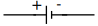
\includegraphics{1_a_pa_source}}
\item one or more resistors (like any appliance that you plug into a wall outlet), denoted by\\
\resizebox{!}{0.25in}{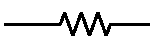
\includegraphics{1_a_pa_resistor}}.
\end{itemize}

The source creates a charge that produces potential energy $E$ measured in volts (V). No substance conducts electricity perfectly, there is always some price to pay (energy loss) to moving electricity. Electrical current $I$ in amperes (A) is the flow of the electric charge in the circuit. (A current of 1 ampere means that $6.2 \times 10^{18}$ electrons pass through the circuit per second.) Current flows out of the positive terminal of a source and runs through each branch of the circuit. Let $I_1$ be the current flowing through the upper branch, $I_2$ the current through middle branch, and $I_3$ the current through the lower branch as illustrated in Figure \ref{F:circuit1}. The goal is to find the current flowing in each branch of the circuit.  

Linear algebra comes into play when analyzing a circuit based on the relationship between current, resistance, and potential. Three basic principles govern current low in a circuit.
\begin{enumerate}
\item Resistance $R$ in ohms ($\Omega$) can be thought of as a measure of how difficult it is to move a charge along a circuit. When a current flows through a resistor, it must expend some energy, called a \emph{voltage drop}. Ohm's Law\index{Ohm's Law} states that the voltage drop $E$ across a resistor is the product of the current $I$ passing through the resistor and the resistance $R$. That is,
\[E = IR.\]
\item Kirchoff's Current Law\index{Kirchoff's Current Law} states that at any point in an electrical circuit, the sum of currents flowing into that point is equal to the sum of currents flowing out of that point.
\item Kirchoff's Voltage Law\index{Kirchoff's Voltage Law} says that around any closed loop the sum of the voltage drops is equal to the sum of the voltage rises. 
\end{enumerate} 

To see how these laws allow us to model the circuit in Figure \ref{F:circuit1}, we will need three equations in $I_1$, $I_2$, and $I_3$ to determine the values of these currents. Let us first apply Kirchoff's Current Law to the point P. The currents flowing into point P are $I_1$ and $I_3$, and the current flowing out is $I_2$. This produces the equation $I_1+I_3 = I_2$, or 
\[I_1 - I_2 + I_3 = 0.\]

\begin{pactivity} Apply Kirchoff's Current Law to the point $Q$ to obtain an equation in $I_1$, $I_2$, and $I_3$. What do you notice?
\end{pactivity}

We have three variables to determine, so we still need two more equations in $I_1$, $I_2$, and $I_3$. Next we apply Kirchoff's Voltage Law to the top loop in the circuit in Figure \ref{F:circuit1}. We will assume the following sign conventions:
\begin{itemize}
\item A current passing through a resistor produces a voltage drop if it flows in the direction of loop (and a voltage rise if the current passes in the opposite direction of the loop). 
\item A current passing through a source in the direction of the loop produces a voltage drop if it flows from $+$ to $-$ and a voltage rise if it flows from $-$ to $+$, while a current passing through a source in the opposite direction of the loop produces a voltage rise if it flows from $+$ to $-$ and a voltage drop if it flows from $-$ to $+$. 
\end{itemize}
(The directions chosen in Figure \ref{F:circuit1} for the voltage flow are arbitrary -- if we reverse the flow then we just replace voltage drops with voltage rises and obtain the same equations. If a solution shows that a current is negative, then that current flows in the direction opposite of what is shown.) 

If we move in the counterclockwise direction around the top loop in the circuit in Figure \ref{F:circuit1}, there is a voltage rise through the source of 8 volts. This must equal the voltage drop in this loop. The current $I_1$ passing though the resistor of resistance 2 $\Omega$ produces a voltage drop of $2I_1$ volts. Similarly, the current $I_1$ passing through the resistor of resistance $3 \Omega$ produces a voltage drop of $3I_1$ volts. Finally, the current $I_2$ passing through the resistor of resistance 2 $\Omega$ produces a voltage drop of $2I_2$ volts. So Kirchoff's Voltage Law applied to the top loop in the circuit in Figure \ref{F:circuit1} gives us the equation $2I_1 + 3I_1 + 2I_2 = 8$ or 
\[5I_1 + 2I_2 = 8.\]

\begin{pactivity} Apply Kirchoff's Voltage Law to the bottom loop in the circuit in Figure \ref{F:circuit1} to obtain an equation in $I_1$, $I_2$, and $I_3$. Compare the three equations we have found to those in the introduction.
\end{pactivity}
 
\begin{figure}[h]
\begin{center}
\resizebox{!}{2.0in}{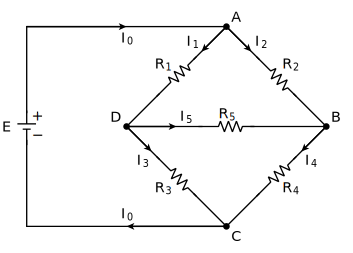
\includegraphics{Wheatstone}}
\end{center}
\caption{A Wheatstone bridge circuit.}
\label{F:Wheatstone}
\end{figure}

\begin{pactivity} Consider the circuit as shown in Figure \ref{F:Wheatstone}, with a single source and five resistors with resistances $R_1$, $R_2$,  $R_3$, $R_4$, and $R_5$ as labeled. 
\ba
\item Assume the following information. The voltage $E$ is $13$ volts, $R_1=R_2=R_3=R_5= 1 \Omega$, and $R_4 = 2  \Omega$. Follow the directions given to find the currents $I_0$, $I_1$, $I_2$, $I_3$, $I_4$, and $I_5$. 
	\begin{enumerate}[i.]
	\item Use Kirchoff's Current Law to show that $I_0 = I_1+I_2$, $I_3 = I_1-I_5$, and  $I_4 = I_2 + I_5$. Thus, we reduce the problem to three variables. 

	\item Apply Kirchoff's Voltage Law to three loops to show that the currents must satisfy the linear system 
\begin{alignat}{4}
{2}I_1	&{}{}		&{}	 	&{}-{}	&{}I_5 	&= & \ 13&{}   \label{eq:Wheatstone_1} \\ 
{}	 	&{}{}		&{3}I_2 	&{}+{}	&{2}I_5 	&= & \ 13&{}  \label{eq:Wheatstone_2}  \\ 
{}I_1 	&{}-{}	&{}I_2 	&{}+{}	&{}I_5 	&= & \ 0&{.}   \label{eq:Wheatstone_3} 
\end{alignat}

	\item Solve the system to find the unknown currents.
	

	\end{enumerate}

\item The circuit pictured in Figure \ref{F:Wheatstone} is called a \emph{Wheatstone bridge} (invented by Samuel Hunter Christie in 1833 and popularized by Sir Charles Wheatstone in 1843). The Wheatstone bridge is a circuit designed to determine an unknown resistance by balancing two paths in a circuit. It is set up so that the resistances of resistors $R_1$ and $R_2$ are known, $R_3$ is a variable resistor and we want to find the resistance of $R_4$. The resistor $R_5$ is replaced with a voltmeter, and the resistance of $R_3$ is varied until the voltmeter reads $0$. This balances the circuit and tells the resistance of resistor $R_4$. Show that if the current $I_5$ in Figure \ref{F:Wheatstone} is $0$ (so the circuit is balanced), then $R_4 = \frac{R_2R_3}{R_1}$ (which is how we calculate the unknown resistance $R_4$). Do this in general and do not use any specific values for the resistances or the voltage. 


\ea
\end{pactivity}


  %1
\achapter{2}{The Matrix Representation of a Linear System} \label{sec:matrix_representation}


\vspace*{-17 pt}
\framebox{
\parbox{\dimexpr\linewidth-3\fboxsep-3\fboxrule}
{\begin{fqs}
\item What is a matrix?
\item How do we associate a matrix to a system of linear equations?
\item What row operations can we perform on an augmented matrix of a linear system to solve the system of linear equations?
\item What are pivots, basic variables, and free variables? 
\item How many solutions can a system of linear equations have?
\item When is a linear system consistent?
\item When does a linear system have infinitely many solutions? A unique solution?
\item How can we represent the set of solutions to a consistent system if the system has infinitely many solutions?
\end{fqs}}}% \hspace*{3 pt}}

\vspace*{13 pt}

\csection{Application: Approximating Area Under a Curve}

We know from basic geometry how to find areas of circles and triangles. However, it is much more difficult to find areas of other geometric objects. In fact, it is generally an impossible problem to determine the exact area bounded by a complicated curve. For this reason, approximation methods are used. One such method involves approximating curves using quadratic functions.

Unless you have learned some calculus, you have probably never calculated the area under a parabola. In the ancient work \emph{Quadrature of the Parabola} (3rd century BC), Archimedes determined a method for finding the area of a region bounded by a parabola by using mechanics and then by geometric methods. Once we know how to calculate the area of a region bounded by a parabola, Simpson's Rule uses parabolas to approximate a function, and then approximates the area under the graph of the graph of the function by using the areas under the parabolas. In order to use Simpsons Rule, we need to know how to exactly fit a quadratic function to three points. More details about this process can be found at the end of this section. This idea of fitting a polynomial to a set of data points has uses in other areas as well. For example, two common applications of B\'{e}zier curves are font design and drawing tools. When fitting a polynomial to a large set of data points, our systems of equations can become quite large, and can be difficult to solve by hand.  In this section we will see how to use matrices to more conveniently represent systems of equations of any size. We also consider how the elimination process works on the matrix representation of a linear system and how we can determine the existence of solutions and the form of solutions of a linear system.

\csection{Introduction}

When working with a linear system, the labels for the variables are irrelevant to the solution -- the only thing that matters is the coefficients of the variables in the equations and the constants on the other side of the equations. For example, given a linear system of the form

\begin{equation}  \label{eq:PA_1}
\begin{alignedat}{4}
a_2 	&{}-{} 	&a_1 	&{}+{}	&a_0 &= 2 \\
a_2 	&{}+{} 	&a_1 	&{}+{} 	&a_0 &= 6 \\
4a_2	&{}+{} 	&2a_1 	&{}+{} 	&a_0	&= 5, 
\end{alignedat}
\end{equation}
the important information in the system can be represented as
\[\begin{tabular}{crcc}
1 &$-1$ &1 &2 \\
1 & 1 &1 &6 \\
4 & 2	&1 &5
\end{tabular}\]
where we interpret the first three numbers in each horizontal row to represent the coefficients of the variables $a$, $b$ and $c$, respectively, and the last number to be the constant on the right hand side of the equation. This tells us that we can record all the necessary information about our system in a rectangular array of numbers. Such an array is called a \emph{matrix}.



\begin{definition} A \textbf{matrix}\index{matrix} is a rectangular array of quantities or expressions.
\end{definition}



We usually delineate a matrix by enclosing its entries in square brackets $[ * ]$. For the system in \eqref{eq:PA_1}, there are two corresponding matrices: 
\begin{center}
\begin{minipage}{2.0in}
\begin{center}
$\left[ \begin{array}{rrr} 1 	&-1 	&1 	\\ 1	&1		&1	\\ 4	&2		&1 \end{array} \right]$ 
\end{center}
\end{minipage}
\begin{minipage}{2.0in}
\begin{center}
$\left[ \begin{array}{rrr|r} 1 	&-1 	&1 &2 	\\ 1	&1		&1 &6	 \\ 4	 &2		&1 &5 \end{array} \right]$
\end{center}
\end{minipage}
\end{center}
The matrix on the left is the matrix of the coefficients of the system, and is called the \emph{coefficient matrix}\index{coefficient matrix} of the system. The matrix on the right is the matrix of coefficients and the constants, and is called the \emph{augmented matrix}\index{augmented matrix} of the system (where we say we augment the coefficient matrix with the additional column of constants). We will separate the augmented column from the coefficient matrix with a vertical line to keep it clear that the last column is an augmented column of constants and not a column of coefficients.\footnote{You should note that not every author uses this convention -- when they do not, it is important that you be careful to understand if the matrix has an augmented column or not.}


\noindent \textbf{Terminology.} There is some important terminology related to matrices.
	\begin{itemize}
	\item Any number in a matrix is called an \emph{entry}\index{matrix!entry} of the matrix. 
	\item The collection of entries in an augmented matrix that corresponds to a given equation (that is reading the entries from left to right, or a horizontal set of entries) is called a \emph{row}\index{matrix!row} of the matrix. We number the rows from top to bottom in a matrix. For example, $\left[ \begin{array}{crc} 1&-1&1 \end{array} \right]$ is the first row and $\left[ \begin{array}{ccc} 1&1&1 \end{array} \right]$ is the second row of the coefficient matrix of the system \eqref{eq:PA_1}.
	\item The set of entries as we read from top to bottom (or a vertical set of entries that correspond to one fixed variable or the constants on the right hand sides of the equations) is called a \emph{column}\index{matrix!column} of the matrix. We number the columns from left to right in a matrix.  For example, $\left[ \begin{array}{c} 1 \\ 1 \\ 4 \end{array} \right]$ is the first column and $\left[ \begin{array}{c} 1 \\ 1 \\ 1 \end{array} \right]$  is the third column of the coefficient matrix of the system \eqref{eq:PA_1}.
	\item The \emph{size}\index{matrix!size} of a matrix is given as $m\times n$ where $m$ is the number of rows and $n$ is the number of columns. The coefficient matrix above is a $3\times 3$ matrix since it has 3 rows and 3 columns, while the augmented matrix is a $3\times 4$ matrix as it has 4 columns.
	\end{itemize}


\begin{pa} \label{pa:1_b} ~
\be 
\item Write the augmented matrix for the following linear system. If needed, rearrange an equation to ensure that the variables appear in the same order on the left side in each equation with the constants being on the right hand side of each equation. 

\begin{equation}
\begin{split}
-x_3 + 3 + 2x_2&= -x_1   \\
-3 + 2x_3 &= -x_2  \\
-2x_2 + x_1 &= 3x_3-7 
\end{split} 
\end{equation} 


\item Write the linear system in variables $x_1, x_2$ and $x_3$, appearing in the natural order that corresponds to the following augmented matrix. Then solve the linear system using the elimination method.

\[\left[ \begin{array}{rrr|r} 1 & 1 & -1 & 4 \\ 1 & 2 & 2 & 3 \\ 2 & 3 & -3 & 11 \end{array} \right]\]


\item Consider the three types of elementary operations on systems of equations introduced in Section \ref{sec:intro_linear_systems}. Each row of an augmented matrix of a system corresponds to an equation, so each elementary operation on equations corresponds to an operation on rows (called row operations). 
	\ba
	\item Describe the row operation that corresponds to interchanging two equations.
	\item Describe the row operation that corresponds to multiplying an equation by a nonzero scalar.
	\item Describe the row operation that corresponds to replacing one equation by the sum of that equation and a scalar multiple of another equation.
	\ea
 

\ee

\end{pa}


\csection{Simplifying Linear Systems Represented in Matrix Form} 

Once we have stored the information about a linear system in an augmented matrix, we can perform the elementary operations directly on the augmented matrix. 

Recall that the allowable operations on a system of equations are the following:
\begin{enumerate}
\item Replacing one equation by the sum of that equation and a scalar multiple of another equation.
\item Interchanging the positions of two equations.
\item Replacing an equation by a nonzero scalar multiple of itself.
\end{enumerate}
Recall that we use these elementary operations to transform a system, with the ultimate goal of finding a simpler, equivalent system that we can solve. Since each row of an augmented matrix corresponds to an equation, we can translate these operations on equations to corresponding operations on rows (called \emph{row operations}\index{row operations} or \emph{elementary row operations}):

\begin{enumerate}
\item Replacing one row by the sum of that row and a scalar multiple of another row.
\item Interchanging two rows.
\item Replacing a row by a nonzero scalar multiple of itself.
\end{enumerate}



\begin{activity} \label{act:A1.2_1} Consider the system 
\begin{alignat*}{4}
{}a_2	&{}-{} 	&{}a_1 	&{}+{}	&{}a_0 	&= 2   \\
{}a_2 	&{}+{}	&{}a_1 	&{}+{}	&{}a_0  &= 6   \\
4a_2 		&{}+{} 	&2a_1 	&{}+{} 	&{}a_0 	&= 5
\end{alignat*} 
with corresponding augmented matrix
\[\left[ \begin{array}{crc|c}
1 	&-1		&1 	&2 \\
1	&1		&1	&6 \\
4	&2		&1	&5
\end{array} \right]
\]
	\ba
	\item As a first step in solving our system, we might eliminate $a_2$ from the second equation. This means that the corresponding entry in the second row and first column of the augmented matrix will become 0. Find a row operation that adds a multiple of the first row to the second row to achieve this goal. Then write the system of equations that corresponds to this new augmented matrix. 

	\item Now that we have eliminated the $a_2$ terms from the second equation, we eliminate the $a_2$ term from the third equation. Find an appropriate row operation that does that, and write the corresponding system of linear equations that corresponds to the new augmented matrix. 

	\item Now you should have a system in which the last two rows correspond to a system of 2 linear equations in two unknowns. Use a row operation that adds a multiple of the second row to the third row to turn the coefficient of $a_1$ in the third row to 0. Then write the corresponding system of linear equations. 

	\item Your simplified system and its augment matrix are in \emph{row echelon form} and this system is solvable using \emph{back-substitution} (substituting the known variable values into the previous equation to find the value of another variable). Solve the system. 	

	\ea

\end{activity}

\begin{reflect}Do you see how this standard elimination process can be generalized to any linear system with any number of variables to produce a simplified system? Do you see why the process does not change the solutions of the system? If needed, can you modify the standard elimination process to obtain a simplified system in which the last equation contains only the variable $a_2$, the next to last equation contains only the variables $a_1, a_2$, etc.? Understanding the standard process will enable you to be able to modify it, if needed, in a problem.
\end{reflect}
 


Activity \ref{act:A1.2_1} illustrates how we can perform all of the operations on equations with operations on the rows of augmented matrices to reduce a system to a solvable form. Each time we perform an operation on the system of equations (or on the rows of an augmented matrix) we obtain an equivalent system (or an augmented matrix corresponding to an equivalent system). For completeness, we list the operations on equations and the corresponding row operations below that can be used to solve our polynomial fitting system. Throughout the process we will let $E_1$, $E_2$, and $E_3$ be the first, second, and third equations in the system and $R_1$, $R_2$, and $R_3$ the first, second, and third rows of the augmented matrices. The notation $E_1+E_2$ placed next to equation $E_2$ means means that we replace the second equation in the system with the sum of the first two equations. We start with the system

\begin{alignat*}{4}
{}a_2	&{}-{} 	&{}a_1 	&{}+{}	&{}a_0 	&= 2   \\
{}a_2 	&{}+{}	&{}a_1 	&{}+{}	&{}a_0  &= 6   \\
4a_2 		&{}+{} 	&2a_1 	&{}+{} 	&{}a_0 	&= 5
\end{alignat*} 



On the left we demonstrate the operations on equations and on the right the corresponding operations on rows of the augmented matrix.


\hspace{-0.2in}
\begin{minipage}{0.7in}
\vspace{0.2in}
{\tiny $E_2-E_1\to E_2$}
\end{minipage}
\hspace{-0.1in}
\begin{minipage}{1.8in}
\vspace{-0.1in}
\begin{alignat*}{4}
{}a_2	&{}-{} 	&{}a_1 	&{}+{}	&{}a_0 	&{}= 2   \\
{}	 	&{}		&2a_1 	&{}		&{}	 	&{}= 4   \\
4a_2 	&{}+{} 	&2a_1 	&{}+{} 	&{}a_0 	&{}= 5
\end{alignat*} 
\end{minipage}
\begin{minipage}{2.35in}
\begin{center}
\renewcommand{\arraystretch}{1.2}
\begin{tabular}{r} \\ \vspace{0.15in}{\tiny $R_2-R_1\to R_2$} \\ \end{tabular} \hspace{-0.1in}$\left[ \begin{array}{rrr|r} 1 &-1 &1 &2 \\ 0 &2 &0 &4 \\ 4 &2&1 &5 \end{array} \right]$
\end{center}
\end{minipage}

\hspace{-0.2in}
\begin{minipage}{0.7in}
\vspace{0.6in}
{\tiny $E_3-4E_1\to E_3$}
\end{minipage}
\hspace{-0.1in}
\begin{minipage}{1.8in}
\vspace{-0.1in}
\begin{alignat*}{4}
{}a_2	&{}-{} 	&{}a_1 		&{}+{}	&{}a_0 	&{}= & \ {}&2   \\
{}	 		&{}		&2a_1 		&{}		&{}	 	&{}= & \ {}&4   \\
{} 		&{} 		&6a_1 		&{}-{} 	&3a_0 	&{}= & \ {-}&3
\end{alignat*} 
\end{minipage}
\begin{minipage}{2.35in}
\begin{center}
\renewcommand{\arraystretch}{1.2}
\begin{tabular}{r} \\ \\ \hspace{0.0in}{\tiny $R_3-4R_1\to R_3$} \end{tabular} \hspace{-0.1in}$\left[ \begin{array}{rrr|r} 1 	 &-1 	&1 &2 	\\ 0	&2		&0 &4	\\ 0	&6		&-3 &-3 \end{array} \right]$
\end{center}
\end{minipage}


\hspace{-0.2in}
\begin{minipage}{0.7in}
\vspace{0.6in}
{\tiny $E_3-3E_2\to E_3$}
\end{minipage}
\hspace{-0.1in}
\begin{minipage}{1.8in}
\vspace{-0.1in}
\begin{alignat*}{5}
{}a_2	&{}-{} 	&{}a_1 		&{}+{}	&{}a_0 	&{}= & \ {}&&{}2   \\
{}	 		&{}		&2a_1 		&{}		&{}	 	&{}= & \ {}&&{}4    \\
{} 		&{} 		&{} 			&{}-{}	&3a_0 	&{}= & \ {-}&&{15}
\end{alignat*} 
\end{minipage}
\begin{minipage}{2.35in}
\begin{center}
\renewcommand{\arraystretch}{1.2}
\begin{tabular}{r} \\ \\ \vspace{0.0in}{\tiny $R_3-3R_2\to R_3$} \\ \end{tabular} \hspace{-0.1in}$\left[ \begin{array}{rrr|r} 1 	 &-1 	&1 &2 	\\ 0	&2		&0 &4	\\ 0	&0		&-3 &-15 \end{array} \right]$
\end{center}
\end{minipage}


Now we can solve the last equation for $a_0$ to find that $a_0=5$. The second equation gives us $a_1 = 2$.\footnote{If there had been an $a_0$ term in the second equation, we could have substituted $a_0=5$ and solved for $a_1$} Finally, using the first equation with the already determined values of $a_0$ and $a_1$ gives us $a_2=-1$. Thus we have found the solution to the polynomial fitting system to be $a_2=-1$, $a_1=2$, and $a_0=5$. 



We summarize the steps of the (partial) elimination on matrices we used above to solve a general linear system in the variables $x_1$, $x_2$, $\ldots$, $x_n$.
\begin{enumerate}
\item Interchange equations if needed to ensure that the coefficient of $x_1$ (or, more generally, the first non-zero variable) in the first equation is non-zero.
\item Use the first equation to eliminate $x_1$ (or, the first non-zero variable) from other equations by adding a multiple of the first equation to the others.
\item After $x_1$ is eliminated from all equations but the first equation, focus on the rest of the equations. Repeat the process of elimination on these equations to eliminate $x_2$  (or, the next non-zero variable) all but the second equation. 
\item Once the process of eliminating variables recursively is finished, solve for the variables in a backwards fashion starting with the last equation and substituting known values in the equations above as they become known.
\end{enumerate}
This elimination method where the variables are eliminated from lower equations is called the \emph{forward elimination phase}\index{forward elimination} as it eliminates variables in the forward direction. Solving for variables using substitution into upper equations is called \emph{back substitution}\index{back substitution}. The matrix representation of a linear system after the forward elimination process is said to be in \emph{row echelon form}. We will define this form and the elimination process on the matrices more precisely in the next section.

\csection{Linear Systems with Infinitely Many Solutions}

Each of the systems that we solved so far have had a unique (exactly one) solution. The geometric representation of linear systems with two equations in two variables shows that this does not always have to be the case. We also have linear systems with no solution and systems with infinitely many solutions. We now consider the problem of how to represent the set of solutions of a linear system that has infinitely many solutions. (Systems with infinitely many solutions will also be of special interest to us a bit later when we study eigenspaces of a matrix.)



\begin{activity} \label{act:A1.2_3} Consider the system  
\begin{alignat*}{4}
{}x_1	&{}+{} 	&{2}x_2		&{}-{}	&{}x_3 	&{}= & \ 1&{} \\
{}x_1	&{}+{}	&{}x_2 		&{}-{}	&{3}x_3	&{}= & \ 0&{}    \\
{2}x_1	&{}+{}	&{3}x_2		&{}-{}	&{4}x_3 &{}= & \ 1&{.}
\end{alignat*} 
	\ba
	\item Without explicitly solving the system, check that $(-1,1,0)$ and $(4,-1,1)$ are solutions to this system. 
	


	\item Without explicitly solving the system, show that $x_1 = -1+5t$, $x_2 = 1-2t$, and $x_3 = t$ is a solution to this system for any value of $t$. What values of $t$ yield the solutions $(-1,1,0)$ and $(4,-1,1)$ from part (a)? The equations $x_1 = -1+5t$, $x_2 = 1-2t$, and $x_3 = t$ form what is called a \emph{parametric solution} to the system with \emph{parameter} $t$. 
	


	\item Part (b) shows that our system has infinitely many solutions. We were given solutions in part (b) -- but how do we find these solutions and how do we know that these are all of the solutions? We address those questions now. 
 
If we apply row operations to the augmented matrix
\[\left[ \begin{array}{ccr|c} 1&2&-1&1 \\ 1&1&-3&0 \\ 2&3&-4&1 \end{array} \right] \]
of this system, we can reduce this system to one with augmented matrix
\[\left[ \begin{array}{ccr|c} 1&2&-1&1 \\ 0&1&2&1 \\ 0&0&0&0 \end{array} \right]. \]
		\begin{enumerate}[i.]
		\item What is it about this reduced form of the augmented matrix that indicates that the system has infinitely many solutions? 
	


		\item Since the system has infinitely many solutions, we will not be able to explicitly determine values for each of the variables. Instead, at least one of the variables can be chosen arbitrarily. What is it about the reduced form of the augmented matrix that indicates that $x_3$ is convenient to choose as the arbitrary variable?



		\item Letting $x_3$ be arbitrary (we call $x_3$ a \emph{free} variable), use the second row to show that $x_2 = 1-2x_3$ (so that we can write $x_2$ in terms of the arbitrary variable $x_3$). 
	


		\item Use the first row to show that $x_1 = 5x_3-1$ (and we can write $x_1$ in terms of the arbitrary variable $x_3$). Compare this to the solutions from part (b). 



		\end{enumerate}
	\ea
	
\end{activity}



After using the elimination method, the first non-zero coefficient (from the left) of each equation in the linear system is in a different position. We call each such coefficient a \emph{pivot} and a variable corresponding to a pivot a \emph{basic variable}. In the system

\begin{alignat*}{5}
{}a_2	&{}-{} 	&{}a_1 		&{}+{}	&{}a_0 	&{}= & \ {}&&{}2   \\
{}	 		&{}		&{2}a_1		&{}		&{}	 	&{}= & \ {}&&{}4    \\
{} 		&{} 		&{} 			&{}-{}	&{3}a_0	&{}= & \ {-}&&{15}
\end{alignat*} 
the basic variables are $a_2, a_1, a_0$ for the first, second, and third equations, respectively. In the system, 

\begin{alignat*}{5}
{}x_1	&{}+{} 	&{2}x_2 	&{}-{}	&{}x_3 	&{}= & \ 1   \\
{}	 		&{}		&{}x_2 		&{}+{}	&{2}x_3	&{}= & \ 1    \\
{} 		&{} 		&{} 			&{}		&{}0 	&{}= & 0
\end{alignat*} 
the basic variables are $x_1$ and $x_2$ for the first and second equations, respectively, while the third equation does not have a basic variable. Through back-substitution, we can solve for each variable in a unique way if each appears as the basic variable in an equation. If, however, a variable is \emph{free}, meaning that it is not the basic variable of an equation, we cannot solve for that variable explicitly. We instead assign a distinct parameter to each such free variable and solve for the basic variables in terms of these parameters. 



\begin{definition} The first non-zero coefficient (from the left) in an equation in a linear system after elimination is called a \textbf{pivot}\index{pivot}. A variable corresponding to a pivot is a \textbf{basic variable}\index{basic variable} and while a variable not corresponding to a pivot is a \textbf{free variable}\index{free variable}.
\end{definition}

\begin{activity} \label{act:A1.2_4} Each matrix is an augmented matrix for a linear system after elimination. Identify the basic variables (if any) and free variables (if any). Then write the general solution (if there is a solution) expressing all variables in terms of the free variables. Use any symbols you like for the variables. 
	\ba
	\item $\left[ \begin{array}{ccc|c} 1&0&2&1 \\ 0&3&1&0 \\ 0&0&0&0 \end{array} \right]$



	\item $\left[ \begin{array}{ccr|c} 1&0&-1&1 \\ 0&0&1&2 \\ 0&0&0&0 \end{array} \right]$
	


	\item $\left[ \begin{array}{ccrc|c} 1&2&-1&1&1 \\ 0&1&0&2&1 \\ 0&0&0&0&0 \\ 0&0&0&0&0 \end{array} \right]$
	

	\ea

\end{activity}



\begin{reflect} Does the existence of a row of 0's always mean a free variable? Can you think of an example where there is a row of 0's but none of the variables is free? How do the numbers of equations and the variables compare in that case?
\end{reflect}




\csection{Linear Systems with No Solutions}

We saw in the previous section that geometrically two parallel and distinct lines represent a linear system with two equations in two unknowns which has no solution. Similarly, two parallel and distinct planes in three dimensions represent a linear system with two equations in three unknowns which has no solution. We can have at least four different geometric configurations of three planes in three dimensions representing a system with no solution. But how do these geometrical configurations manifest themselves algebraically? 

\begin{activity} Consider the linear system
\begin{alignat*}{4}
x_1 		&{}-{}	&x_2 	&{}+{}	&{}x_3	&{}={} & \ 2 &{} \\
x_1		&{}+{}	&x_2	&{}-{}	&{3}x_3	&{}={} & \ 1 &{} \\
{3}x_1	&{}-{}	&x_2	&{}-{}	&{}x_3	&{}={}	& \ 6 &{.}
\end{alignat*}

\ba 
\item Apply the elimination process to the augmented matrix of this system. Write the system of equations that corresponds to the final reduced matrix. 



\item Discuss which feature in the final simplified system makes it easy to determine that the system has no solution. Similarly, what features in the matrix representation makes is easy to see the system has no solution?



\ea

\end{activity}

We summarize our observations about when a system has a solution, and which of those cases has a unique solution.

\begin{theorem}
A linear system is consistent if after the elimination process there is no equation of the form $0=b$ where $b$ is a non-zero number. If a linear system is consistent and has a free variable, then it has infinitely many solutions. If it is consistent and has no free variables, then there is a unique solution.
\end{theorem}



\csection{Examples}

\ExampleIntro

\begin{example} Consider the linear system 
\begin{alignat*}{5}
{}x_1		&{}-{} 	&{ }x_2		&{}{}		&{}		&{}+{}	&{2}x_4 	&{}= & \ 1&{} \\
{2}x_1	&{}+{} 	&{3}x_2		&{}-{}	&{2}x_3	&{}+{}	&{5}x_4 	&{}= & \ 4&{} \\
{}x_1		&{}-{} 	&{}x_2		&{}+{}	&{}x_3	&{}-{}	&{ }x_4 	&{}= & \ 0&{} \\
{4}x_1	&{}+{} 	&{}x_2		&{}-{}	&{}x_3	&{}+{}	&{6}x_4 	&{}= & \ 5&{.} 
\end{alignat*} 
	\ba
	\item Set up the augmented matrix for this linear system.
	
	\item Find all solutions to the system using forward elimination. 
	
	\item Suppose, after forward elimination, the augmented matrix of the system
\begin{alignat*}{5}
{}x_1		&{}-{} 	&{ }x_2		&{}{}		&{}		&{}+{}	&{2}x_4 	&{}= & \ 1&{} \\
{2}x_1	&{}+{} 	&{3}x_2		&{}-{}	&{2}x_3	&{}+{}	&{5}x_4 	&{}= & \ 4&{} \\
{}x_1		&{}-{} 	&{}x_2		&{}+{}	&{}x_3	&{}-{}	&{ }x_4 	&{}= & \ 0&{} \\
{4}x_1	&{}+{} 	&{}x_2		&{}-{}	&{}x_3	&{}+{}	&{6}x_4 	&{}= & \ h&{.} 
\end{alignat*} 
has the form
\[\left[ \begin{array}{crrr|c} 1&-1&0&2&1 \\ 0&5&-2&1&2 \\ 0&0&1&-3&-1 \\ 0&0&0&0&h-5 \end{array} \right].\]
For which values of $h$ does this system have: 
	\begin{enumerate}[i.]
	\item No solutions?
	\item A unique solution? Find the solution.
	\item Infinitely many solution? Determine all solutions? 
	\end{enumerate}
\ea

\ExampleSolution
\ba
\item The augmented matrix for this system is 
\[\left[ \begin{array}{crrr|c} 1&-1&0&2&1 \\ 2&3&-2&5&4 \\ 1&-1&1&-1&0 \\ 4&1&-1&6&5 \end{array} \right].\]
\item We apply forward elimination, first making the entries below the 1 in the upper left all 0. We do this by replacing row two with row two minus 2 times row 1, row three with row three minus row 1, and row four with row four minus 4 row one. This produces the augmented matrix
 \[\left[ \begin{array}{crrr|r} 1&-1&0&2&1 \\ 0&5&-2&1&2 \\ 0&0&1&-3&-1 \\ 0&5&-1&-2&1 \end{array} \right].\]
 Now we eliminate the leading 5 in the fourth row by replacing row four with row four minus row two to obtain the augmented matrix
  \[\left[ \begin{array}{crrr|r} 1&-1&0&2&1 \\ 0&5&-2&1&2 \\ 0&0&1&-3&-1 \\ 0&0&1&-3&-1 \end{array} \right].\]
  When we replace row four with row four minus row three, we wind up with a row of zeros:
  \[\left[ \begin{array}{crrr|r} 1&-1&0&2&1 \\ 0&5&-2&1&2 \\ 0&0&1&-3&-1 \\ 0&0&0&0&0 \end{array} \right].\]  
 We see that there is no pivot in column four, so $x_4$ is a free variable. We can solve for the other variables in terms of $x_4$. The third row shows us that 
 \begin{align*}
 x_3 - 3x_4 &= -1 \\
 x_3 &= 3x_4 - 1.
 \end{align*}
 The second row tells us that
 \begin{align*}
 5x_2 - 2x_3 + x_4 &= 2 \\
 5x_2 &= 2x_3 - x_4 + 2 \\
 5x_2 &= 2(3x_4-1) - x_4 + 2 \\
 5x_2 &= 5x_4 \\
 x_2 &= x_4.
 \end{align*}
 Finally, the first row gives us
 \begin{align*}
 x_1-x_2+2x_4 &= 1 \\
 x_1 &= x_2 - 2x_4 + 1 \\
 x_1 &= x_4 - 2x_4 + 1 \\
 x_1 &= -x_4 + 1.
 \end{align*}
 So this system has infinitely many solutions, with $x_1 = -x_4 + 1$, $x_2 = x_4$, $x_3 = 3x_4 - 1$, and $x_4$ is arbitrary. As a check, notice that 
 \[(-x_4+1) - x_4 + 2x_4 = 1\]
 and so this solution satisfies the first equation in our system. You should check to verify that it also satisfies the other three equations.
 \item 
 	\begin{enumerate}[i.]
	\item The system has no solutions when there is an equation of the form $0 = b$ for some nonzero number $b$. The last row will correspond to an equation of the form $0 = h-5$. So our system will have no solutions when $h \neq 5$. 
	\item When $h \neq 5$, the system has no solutions. When $h = 5$, the variable $x_4$ is a free variable and the system has infinitely many solutions. So there are no values of $h$ for which the system has exactly one solution.
	\item When $h = 5$, the variable $x_4$ is a free variable and the system has infinitely many solutions. The solutions were already found in part (a).
	\end{enumerate}
 
 \ea 
	 
\end{example}

\begin{example} After applying row operations to the augmented matrix of a system of linear equations, each of which describes a plane in 3-space, the following augmented matrix was obtained:
\[\renewcommand{\arraystretch}{1.4} \left[ \begin{array}{ccc|r} 1&a&0&2 \\ 0&2-2a&b&-4 \\ 0&0&3-\frac{1}{2}b&1 \end{array} \right].\]
	\ba
	\item Describe, algebraically and geometrically, all solutions (if any), to this system when $a=0$ and $b=2$. 
	\item  Describe, algebraically and geometrically, all solutions (if any), to this system when $a=0$ and $b=6$. 
	\item  Describe, algebraically and geometrically, all solutions (if any), to this system when $a=1$ and $b=12$. 
	\ea


\ExampleSolution Throughout, we will let the variables $x$, $y$, and $z$ correspond to the first, second, and third columns, respectively, of our augmented matrix.  
\ba
\item When $a=0$ and $b=2$ our augmented matrix has the form 
\[ \left[ \begin{array}{ccc|r} 1&0&0&2 \\ 0&2&2&-4 \\ 0&0&2&1 \end{array} \right].\]
This matrix corresponds to the system
\begin{alignat*}{4}
{}x	&{}{} 		&{}		&{}{}		&{}		 &{}= & \ 2&{} \\
{}	&{}{} 		&{2}y	&{}+{}	&{2}z	 &{}= & \ -4&{} \\
{}	&{}{} 		&{}		&{}{}		&{2}z	&{}= & \ 1&{.} \\
\end{alignat*} 
There are no equations of the form $0 = b$ for a nonzero constant $b$, so the system is consistent. There are no free variables, so the system has a unique solution. Algebraically, the solution is $x = 2$, $z = \frac{1}{2}$, and $y = -\frac{5}{2}$. Geometrically, this tells us that the three planes given by the original system intersect in a single point. 
\item When $a=0$ and $b=6$ our augmented matrix has the form 
\[ \left[ \begin{array}{ccc|r} 1&0&0&2 \\ 0&2&6&-4 \\ 0&0&0&1 \end{array} \right].\]
The last row corresponds to the equation $0 = 1$, so our system is inconsistent and has no solution. Geometrically, this tells us that the three planes given by the original system do not all intersect at any common points.
\item When $a=1$ and $b=12$ our augmented matrix reduces to  
\[ \renewcommand{\arraystretch}{1.4} \left[ \begin{array}{ccc|r} 1&1&0&2 \\ 0&0&1&-\frac{1}{3} \\ 0&0&0&0 \end{array} \right].\]
There are no rows that correspond to equations of the form $0 = c$ for a nonzero constant $c$, so the system is consistent. The variable $y$ is a free variable, so the system has infinitely many solutions. Algebraically, the solutions are $y$ is free, is $z = -\frac{1}{3}$, and $x = 2-y$.  Geometrically, this tells us that the three planes given by the original system intersect in the line with $z = -\frac{1}{3}$, and $x = 2-y$.  

\ea

\end{example}

\csection{Summary}

\begin{itemize}
\item A matrix is just a rectangular array of numbers or objects. 
\item Given a system of linear equations, with the variables listed in the same order in each equation, we represent the system by writing the coefficients of the first equation as the first row of a matrix, the coefficients of the second equation as the second row, and so on. This creates the coefficient matrix of the system. We then augment the coefficient matrix with a column of the constants that appear in the equations. This gives us the augmented matrix of the system. 
\item The operations that we can perform on equations translate exactly to row operations that we can perform on an augmented matrix:
\begin{enumerate}
\item Replacing one row by the sum of that row and a scalar multiple of another row.
\item Interchanging two rows.
\item Replacing a row by a nonzero scalar multiple of itself.
\end{enumerate}
\item The forward elimination phase of the elimination method recursively eliminates the variables in a linear system to reach an equivalent but simplified system.
\item The first non-zero entry in an equation in a linear system after elimination is called a pivot.
\item A basic variable in a linear system corresponds to a pivot of the system. A free variable is a variable that is not basic.
\item A linear system can be inconsistent (no solutions), have a unique solution (if consistent and every variable is a basic variable), or have infinitely many solutions (if consistent and there is a free variable).  
\item A linear system has no solutions if, after elimination, there is an equation of the form $0=b$ where $b$ is a nonzero number.
\item A linear system after the elimination method can be solved using back-substitution. The free variables can be chosen arbitrarily and the basic variables can be solved in terms of the free variables through the back-substitution process.
\end{itemize}



\csection{Exercises}

\be
\item Consider the system of linear equations whose augmented matrix is
\[ \left[ \begin{array}{cc|r} 1 & 3 & -1 \\ 2& h & k \end{array} \right] \]
where $h$ and $k$ are unknown constants. For which values of $h$ and $k$ does this system have 
	\ba
	\item a unique solution, 
	\item infinitely many solutions, 
	\item no solution? 
	\ea

\item Consider the following system:
\begin{alignat*}{5}
{}x 	&{}-{}	&{2}y	&{}+{}	&{}z		&{}={}	&\ {-}&1&{}\\
{-}x	&{}+{}	&{}y		&{}-{}	&{3}z	&{}={} &\ {}&2&{} \\
{}x	&{}+{}	&{h}y	&{}-{}	&{}z		&{}={}	& \ {}&0&{.}
\end{alignat*}
Check that when $h=-3$ the system has infinitely many solutions, while when $h\neq -3$ the system has a unique solution.


\item If possible, find a system of three equations (not in reduced form) in three variables whose solution set consists only of the point $x_1=2, x_2=-1, x_3=0$.

\item What are the possible geometrical descriptions of the solution set of two linear equations in $\R^3$? (Recall that $\R^3$ is the three-dimensional $xyz$-space -- that is, the set of all ordered triples of the form $(x,y,z)$).

\item Two students are talking about when a linear system has infinitely many solutions. 
\begin{quote}
Student 1: So, if we have a linear system whose augmented matrix has a row of zeros, then the system has infinitely many solutions, doesn't it?
\end{quote} 
\begin{quote}
Student 2: Well, but what if there is a row of the form $[\, 0\, 0\, \ldots\, 0\, |\, b\, ]$ with a non-zero $b$ right above the row of 0's?
\end{quote} 
\begin{quote}
Student 1: OK, maybe I should ask ``If we have a consistent linear system whose augmented matrix has a row of zeros, then the system has infinitely many solutions, doesn't it?"
\end{quote} 
\begin{quote}
Student 2: I don't know. It still doesn't sound enough to me, but I'm not sure why.
\end{quote}
Is Student 1 right? Or is Student 2's hunch correct? Justify your answer with a specific example if possible.

\item Label each of the following statements as True or False. Provide justification for your response.
\ba
\item \textbf{True/False} A system of linear equations in two unknowns can have exactly five solutions.

\item \textbf{True/False} A system of equations with all the right hand sides equal to 0 has at least one solution.

\item \textbf{True/False} A system of equations where there are fewer equations than the number of unknowns (known as an underdetermined system) cannot have a unique solution.

\item \textbf{True/False} A system of equations where there are more equations than the number of unknowns (known as an overdetermined system) cannot have a unique solution.

\item \textbf{True/False} A consistent system of two equations in three unknowns cannot have a unique solution.

\item \textbf{True/False} If a system with three equations and three unknowns has a solution, then the solution is unique.

\item \textbf{True/False} If a system of equations has two different solutions, then it has infinitely many solutions.

\item \textbf{True/False} If there is a row of zeros in the row echelon form of the augmented matrix of a system of equations, the system has infinitely many solutions.

\item \textbf{True/False} If there is a row of zeros in the row echelon form of the augmented matrix of a system of $n$ equations in $n$ variables, the system has infinitely many solutions.

\item \textbf{True/False} If a system has no free variables, then the system has a unique solution.

\item \textbf{True/False} If a system has a free variable, then the system has infinitely many solutions.

\ea

\ee

\csection{Project: Polynomial Interpolation to Approximate the Area Under a Curve} \label{sec:1_b_polynomial}

Suppose we want to approximate the area of the region shown in Figure \ref{F:1_b_area}. As discussed in the introduction, we can approximate the area under a curve by approximating the curve by quadratics. First, we will see how Archimedes approached the problem of finding the area of a quadratic region, then we will determine how to determine a quadratic function that passes through three points, then we put it all together to approximate the area under a curve as in Figure \ref{F:1_b_area}. 

\begin{figure}[h]
\begin{center}
\resizebox{!}{2.5in}{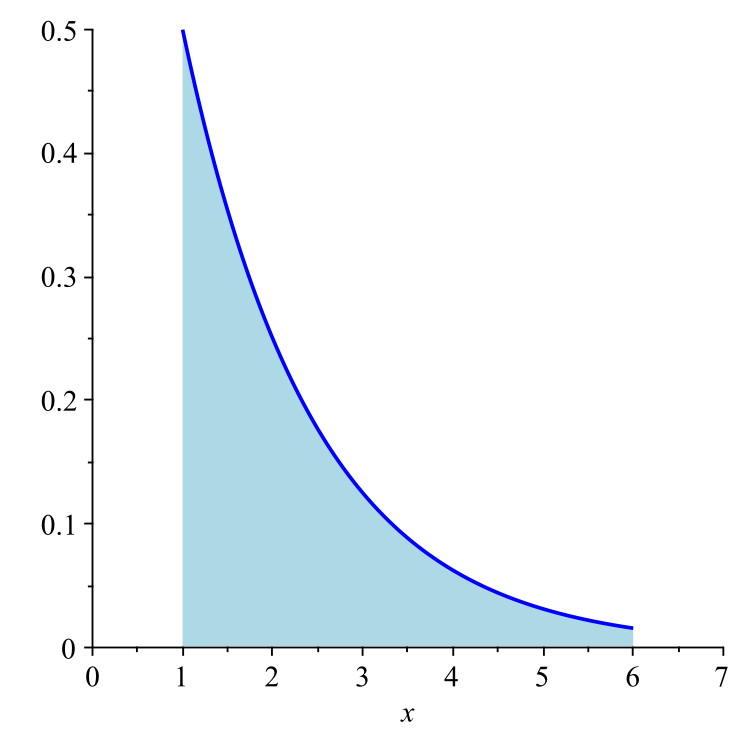
\includegraphics{1_b_area.eps}}
\end{center}
\caption{A region whose area we want to approximate.}
\label{F:1_b_area}
\end{figure}

Archimedes approached the problem of calculating the area of a quadratic region in the following way. Given a quadratic $q(x)$ on an interval $[a,b]$, Archimedes drew in a base given by the secant line connecting the points $(a,q(a))$ and $(b,q(b))$ as illustrated at left in Figure \ref{F:1_b_Archimedes}. Then he found the point in the interval $[a,b]$ at which the tangent line to the curve is parallel to the secant line. Archimedes gave an argument using mechanics (based on balance points), and then another using geometry (through a method of exhaustion) to show that the area of the parabolic region is $\frac{4}{3}$ times the area of the triangle determined by the endpoints and the point of tangency as shown at right in Figure \ref{F:1_b_Archimedes}.
\begin{figure}[h]
\begin{center}
\resizebox{!}{2.0in}{\includegraphics{1_b_Archimedes_1.eps}} \hspace{0.5in} \resizebox{!}{2.0in}{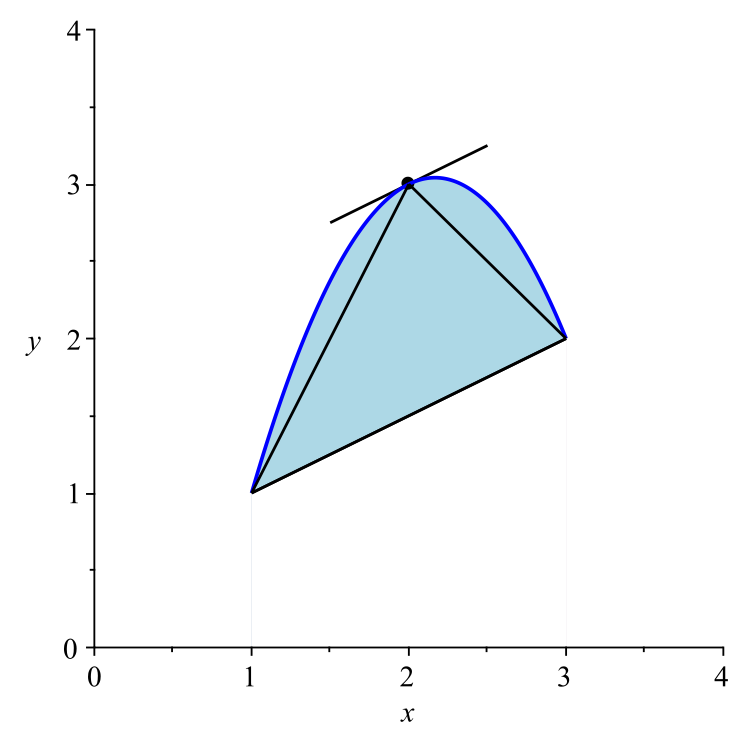
\includegraphics{1_b_Archimedes_2.eps}}
\end{center}
\caption{Archimedes method.}
\label{F:1_b_Archimedes}
\end{figure}
Although we won't go through the details, a conclusion we can draw from Archimedes argument, using the formula for the area of a rectangle and the area of a triangle, is that the area between the graph of a quadratic with equation $q(x) = ax^2+bx+c$ and the $x$-axis on an interval $[x_1, x_2]$ as illustrated in Figure \ref{F:1_b_quad_area} is 
\begin{equation} \label{eq:quad_area}
\frac{a}{3}(x_2^3-x_1^3) + \frac{b}{2}(x_2^2-x_1^2) + c(x_2-x_1).
\end{equation}
\begin{figure}[h]
\begin{center}
\resizebox{!}{2.5in}{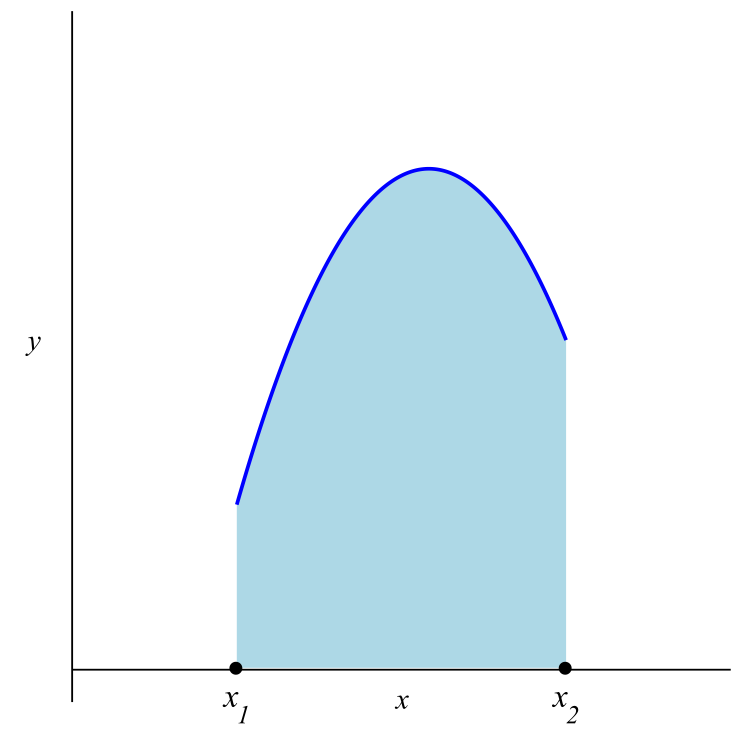
\includegraphics{1_b_quad_area.eps}} 
\end{center}
\caption{Region between a parabola and the $x$-axis.}
\label{F:1_b_quad_area}
\end{figure}
To approximate the area under the graph of a function, we will approximate the function itself with a collection of quadratics, and then use equation (\ref{eq:quad_area}) repeatedly. To do this, we need to know how to fit a quadratic curve to a three points. We consider that question now.

Suppose we are given a collection of three points in the plane: $(x_1, y_1), (x_2, y_2)$ and $(x_3, y_3)$. There is exactly one quadratic polynomial $p(x)$ which goes through these points, i.e. there is exactly one quadratic $p(x)$ such that for each $x_i$, $p(x_i)=y_i$. This is an example of \emph{polynomial curve fitting}\index{polynomial curve fitting}. 

As an example, we use the points $(-1, 2)$, $(1,6)$, $(2,5)$. To fit a quadratic to these points, consider a general quadratic of the form $p(x)=a_2x^2+a_1x+a_0$. By substituting the $x$ value of each of the given points and setting that equal to the $y$ value of that point, we find three equations
\[ (-1)^2a_2-a_1+a_0=2 \; , \; \quad a_2+a_1+a_0=6 \; , \; \quad (2)^2a_2 +2a_1+a_0=5 \]
that give us a system of three equations in the three unknowns $a_2$, $a_1$, and $a_0$:
\begin{alignat*}{4}
{}a_2	&{}-{} 	&{}a_1 	&{}+{}	&{}a_0 	&= 2   \\
{}a_2 	&{}+{}	&{}a_1 	&{}+{}	&{}a_0  &= 6   \\
{4}a_2	&{}+{} 	&{2}a_1	&{}+{} 	&{}a_0 	&= 5. 
\end{alignat*} 
This system is the example we considered in Preview Activity \ref{pa:1_b}, whose solution is $a_2 = -1$, $a_1=2$, and $a_0 = 5$. A graph of $q(x) = -x^2+2x+5$ along with the three points $(-1, 2)$, $(1,6)$, $(2,5)$ is shown in Figure \ref{F:1_b_quadratic_fit}. 
\begin{figure}[h]
\begin{center}
\resizebox{!}{2.5in}{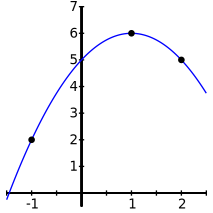
\includegraphics{1_b_quadratic_fit.eps}}
\end{center}
\caption{A quadratic fit to the points $(-1, 2)$, $(1,6)$, $(2,5)$.}
\label{F:1_b_quadratic_fit}
\end{figure}

Now that we know how to fit a quadratic to three points, we next approximate a curve with a collection of quadratics. The method we use is to break the interval on which our curve is defined into several subintervals and create quadratics on each subinterval. The basic idea is contained in our first project activity.
 
\begin{pactivity} \label{act:1_b_Simpson_ex_1}  In this activity we model the function $f$ defined by $f(x) = \sin(2x)+2$ on the interval $[a,b]$, where $a = -\frac{\pi}{2}$ and $b = \pi$ with a collection of quadratics. Let $f(x) = \sin(x)$. We divide the interval $[a,b]$ into three subintervals using the six points $x_0 = -\frac{\pi}{2}$, $x_1 = -\frac{\pi}{4}$, $x_2 = 0$, $x_3 = \frac{\pi}{4}$, $x_4 = \frac{\pi}{2}$, $x_5 = \frac{3 \pi}{4}$, and $x_6 = \pi$. We need three points to determine a quadratic, so the three subintervals of the interval $[a,b]$ will be the intervals $[x_0, x_2]$, $[x_2, x_4]$, and $[x_4,x_6]$. An illustration of the process of dividing our interval $[a,b]$ and approximating by quadratics can be found at \url{https://www.geogebra.org/m/spd4hhbw}. Round all calculations in this activity to the nearest thousandth.
	\ba
	\item Set up a system of linear equations to fit a quadratic $q_1(x) = r_1x^2+s_1x+t_1$ to the three points $(x_0, f(x_0))$, $(x_1, f(x_1))$, and $(x_2, f(x_2))$.  (The solution to this system to the nearest thousandth is $r_1 = 2$, $s_1 \approx 2.546$, and $t_1 = 1.621$.) 

	\item Set up a system of linear equations to fit a quadratic $q_2(x) = r_2x^2+s_2x+t_2$ to the three points $(x_2, f(x_2))$, $(x_3, f(x_3))$, and $(x_4, f(x_4))$. (The solution to this system to the nearest thousandth is $r_2 = 2$, $s_2 \approx  2.546$, and $t_2 \approx  -1.621$.)
	
	\item Set up a system of linear equations to fit a quadratic $q_3(x) = r_3x^2+s_3x+t_3$ to the 3 points $(x_4, f(x_4))$, $(x_5, f(x_5))$, and $(x_6, f(x_6))$. (The solution to this system to the nearest thousandth is $r_3 \approx 10.000$, $s_3 \approx  -7.639$, and $t_3 \approx  1.621$.)
	
	\item Use the GeoGebra applet at \url{https://www.geogebra.org/m/spd4hhbw} to graph the three quadratics on their intervals on the same axes as the graph of $f$. Explain what you see.

	\ea
\end{pactivity}  	

Project Activity \ref{act:1_b_Simpson_ex_1} illustrates how we can model a function on an interval using a sequence of quadratic functions. Now we apply this polynomial curve fitting technique to derive the general formula for approximating the area between a graph of a function $f$ and the $x$-axis. We use parabolic arcs to approximate the graph of $f$ on each subinterval. 

We start by dividing the interval $[a,b]$ over which our function is defined into some number of subintervals. We need an even number of subintervals, since we have to use three points to define each parabola. Let $n = 2m$ be the number of subintervals we use. In order to make the calculations a bit easier, let the subintervals all have the same length, which we denote by $\Delta x$ (the symbol $\Delta$ is often used in mathematics to indicate a change in a quantity). Since we have $n$ subintervals, the length of each subinterval will be $\Delta x = \frac{b-a}{n}$.  For each $k$ we let $x_k = a+k \Delta x$ and $y_k = f(x_k)$. Note that $x_0 = a$ and $x_n=b$. This labeling scheme is illustrated in Figure \ref{F:1_b_partition}
\begin{figure}[h]
\begin{center}
\resizebox{!}{2.5in}{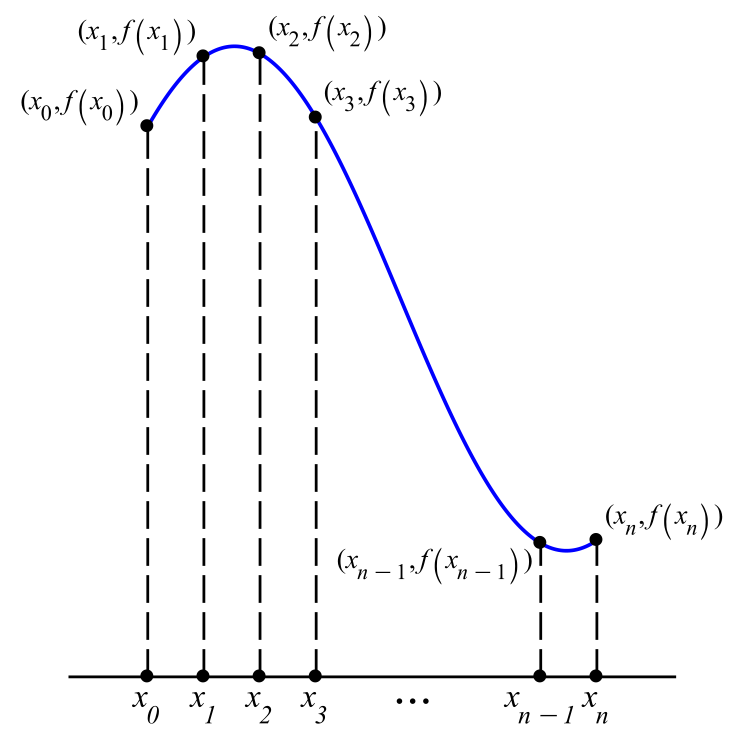
\includegraphics{1_b_partition.eps}}
\end{center}
\caption{Subdividing the interval $[a,b]$.}
\label{F:1_b_partition}
\end{figure}

We approximate $f$ on each subinterval using a quadratic. So we need to find the quadratic $Q(x) = c_2x^2+c_1x+c_0$ that passes through two consecutive end points as well as the midpoint of a subinterval. That is, we need to find the coefficients of $Q$ so that $Q$ passes through the points $(x_k,y_k)$, $(x_{k+2}, y_{k+2})$, and the midpoint $(x_{k+1},y_{k+1})$ on the interval $[x_k, x_{k+2}]$ (so that we have three points to which to fit a parabola) as shown at left in Figure \ref{F:1_b_quad_fit}. Note that the length of the interval $[x_k, x_{k+2}]$ is $2\Delta x$.  To make the calculations easier, we will translate our function so that our leftmost point is $(-r, y_k)$. Then the middle point is $(0, y_{k+1})$ and the rightmost point is $(r, y_{k+2})$ as illustrated at right in Figure \ref{F:1_b_quad_fit}, where $r = \Delta x$.   
\begin{figure}[h]
\begin{center}
\resizebox{!}{2.0in}{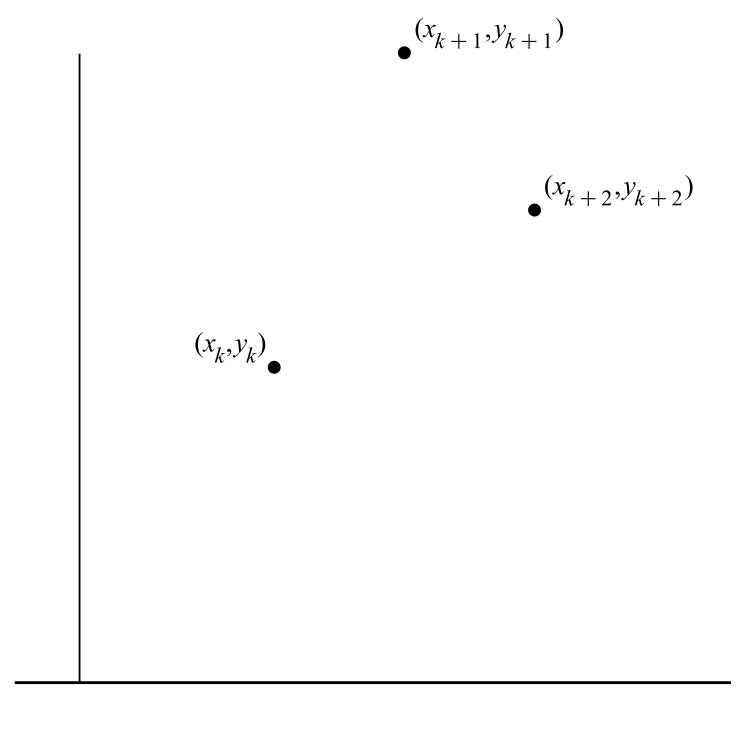
\includegraphics{1_b_quad_fit.eps}} \hspace{0.5in} \resizebox{!}{2.0in}{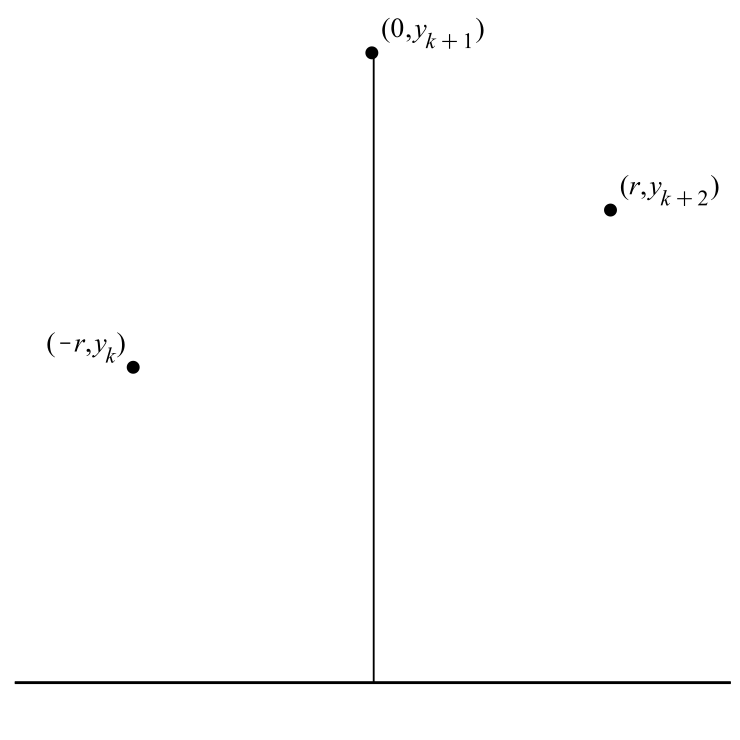
\includegraphics{1_b_translate.eps}}
\end{center}
\caption{Left: Three points. Right: Translated points.}
\label{F:1_b_quad_fit}
\end{figure}


\begin{pactivity} ~
	\ba
	\item Set up a linear system that will determine the coefficients $c_2$, $c_1$,  and $c_0$ so that the polynomial $Q(x) = c_2x^2+c_1x+c_0$ passes through the points $(-r, y_k)$, $(0, y_{k+1})$,  and $(r, y_{k+2})$ with $r \neq 0$. Remember that the unknowns in this system are $c_2$, $c_1$, and $c_0$. 

	\item Explain why the coefficient matrix of the system in part (a) is $\left[ \begin{array}{crc} r^2&-r&1 \\ 0&0&1 \\ r^2&r&1 \end{array} \right]$. Then explain why row reducing the matrix $\left[ \begin{array}{crcc} r^2&-r&1&y_k \\ 0&0&1&y_{k+1} \\ r^2&r&1&y_{k+2} \end{array} \right]$ will find the coefficients we want. Assume that a row echelon form of the matrix $\left[ \begin{array}{crcc} r^2&-r&1&y_k \\ 0&0&1&y_{k+1} \\ r^2&r&1&y_{k+2} \end{array} \right]$ is 
\[\left[ \begin{array}{crcc} r^2&-r&1&y_k \\ 0&2r&0&y_{k+2}-y_k \\ 0&0&1&y_{k+1} \end{array} \right].\]
Use these matrices to explain why $c_2=\frac{y_k-2y_{k+1}+y_{k+2}}{2r^2}$, $c_1=\frac{y_{k+2}-y_k}{2r}$, and $c_0 = y_{k+1}$. 

	\item Our goal is to ultimately approximate the area under the curve on the interval $[a,b]$ by approximating $f$ with quadratics on each subinterval. Use the Archimedean formula (\ref{eq:quad_area}) to show that the area under the quadratic $Q(x)$ from part (a) is 
\[\frac{1}{3}  \left(y_k+4y_{k+1}+y_{k+2}\right) \Delta x.\]

	\item Now add up all of the area approximations on each subinterval to show that the approximate area under the graph is given by the formula 
\begin{equation} \label{eq:1_b_Simpson_sum} 
S(n) = \left(y_0 + 4y_1 + 2y_2 + 4y_3 + 2y_4 + \cdots 2y_{n-2} + 4y_{n-1} + y_n\right) \frac{\Delta x}{3}.
\end{equation}


	\ea
	
\end{pactivity}

We conclude with an example.

\begin{pactivity} Let $f(x) = \left(\frac{1}{2}\right)^x$ on the interval $[1,6]$. A graph of $f$ is shown in Figure \ref{F:1_b_area}. Use our approximation formula with $n=8$ to approximate the area of the shaded region in Figure \ref{F:1_b_area}. Show all of your work and round all calculations to the nearest thousandth. 

\end{pactivity}



 %2
\achapter{3}{Row Echelon Forms} \label{sec:row_echelon_forms}

\vspace*{-17 pt}
\framebox{
\parbox{\dimexpr\linewidth-3\fboxsep-3\fboxrule}
{\begin{fqs}
\item What is the row echelon form of a matrix?
\item What is the procedure to obtain the row echelon form of any matrix?
\item What is the reduced row echelon form of a matrix?
\item What is the procedure to obtain the reduced row echelon form of any matrix?
\item What do the echelon forms of the augmented matrix for a linear system tell us about the solutions to the system?
\end{fqs}}}% \hspace*{3 pt}}

\vspace*{13 pt}

\csection{Application: Balancing Chemical Reactions}

Linear systems have applications in chemistry when balancing chemical equations. When a chemical reaction occurs, molecules of different substances combine to create molecules of other substances. Chemists represent such reactions with chemical equations. To balance a chemical equation means to find the number of atoms of each element involved that will preserve the number of atoms in the reaction. 
As an example, consider the chemical equation
\begin{equation}
\text{C}_2\text{H}_6 + \text{O}_2 \to \text{CO}_2 + \text{H}_2\text{O}. \label{eq:reaction1}
\end{equation}
This equation asks about what will happen when the chemicals ethane ($\text{C}_2\text{H}_6$) and oxygen ($\text{O}_2$), called the \emph{reactants} of the reaction, combine to produce carbon dioxide ($\text{CO}_2$) and water ($\text{H}_2\text{O}$), called the \emph{products} of the reaction (note that oxygen gas is \emph{diatomic}, so that oxygen atoms are paired). The arrow indicates that it is the reactants that combine to form the products. Any chemical reaction has to obey the Law of Conservation of Mass that says that mass can neither be created nor destroyed in a chemical reaction. Consequently, a chemical reaction requires the same number of atoms on both sides of the reaction. In other words, the total mass of the reactants must equal the total mass of the products. In reaction (\ref{eq:reaction1}) the chemicals involved are made up of carbon (C), hydrogen (H), and oxygen (O) atoms. To balance the equation, we need to know how many molecules of each chemical are combined to preserve the number of atoms of C, H, and O. This can be done by setting up a linear system of equations of the form 
\begin{alignat*}{5}
{2}x_1 	&{}		&{}		&{}-{}	&{}x_3	&{}		&{} 			&{}={}	& \ 0&{}   \\
{6}x_1	&{} 		&{} 		&{}		&{}		&{}-{}	&{2}x_4 	&{}={} 	& \ 0&{} \\
{}			&{}		&{2}x_2	&{}-{} 	&{2}x_3	&{}-{}	&{}x_4		&{}={} 	& \ 0&{,}
\end{alignat*}
where $x_1$, $x_2$, $x_3$, and $x_4$ represent the number of molecules of $\text{C}_2\text{H}_6$,  $\text{O}_2$,  $\text{CO}_2$, and $\text{H}_2\text{O}$, respectively, in the reaction and then solving the system. Specific details can be found at the end of this section. 

\csection{Introduction}

In the previous sections, we identified operations on a given linear system with corresponding equivalent operations on the matrix representations which simplify the system and its matrix representation without changing the solutions of the system. Our end goal was to obtain a system which could be solved using back substitution, such as 

\begin{alignat*}{4}
{}x_1 	&{}-{} 	&{}x_2 	&{}+{} 	&{}x_3 &{}={}	&0&{}   \\
{}			&{} 		&{6}x_2 &{}-{}	&{}x_3 &{}={} 	&8&{} \\
{}			&{}		&{}		&{}	 	&{}x_3 &{}={} 	&1&{.} 
\end{alignat*}
The augmented matrix for this system is
\[ \left[ \begin{array}{crr|c} 1 &-1 &1 &0 \\ 0& 6 &-1 &8 \\ 0&0 &1 &1 \end{array} \right]. \]
The matrices of linear systems which can be solved via back substitution are said to be in \emph{row echelon form} (or simply \emph{echelon form}). We will define the properties of matrices in this form precisely in this section. Our goal will be to prescribe a precise procedure for converting any matrix to an equivalent one in row echelon form without having to convert back to the system representation.

\begin{pa} \label{pa:1_c}  We want to determine a suitable form for an augmented matrix that can be obtained from row operations so that it is straightforward to find the solutions to the system. We begin with some examples.

\be
\item Write the linear system corresponding to each of the following augmented matrices. Use the linear system to determine which systems have their variables eliminated completely in the forward direction, or equivalently determine for which systems the next step in the solution process is back substitution (possibly using free variables). Explain your reasoning. You do not need to solve the systems. 
	\begin{enumerate}[i.]
	\begin{minipage}{2.0in}
	\item $\ds \left[ \begin{array}{rrc|r} 1 & -1 & 2 & -2 \\ 0 & 1 & 2& -1 \\ 0 & 0 & 3 & 1   \end{array} \right]$
	\end{minipage}
	\begin{minipage}{2.0in}
	\item $\ds \left[ \begin{array}{crc|r} 1 & 1 & 0 & -2 \\ 0 & 1 & 0 & 3  \\ 0 & 0 & 0& 0 \end{array} \right]$
	\end{minipage}
	
	\begin{minipage}{2.0in}
	\item $\ds \left[ \begin{array}{ccc|c} 1 & 1 & 1 & 2 \\ 1 & 2 & 2 & 2  \\ 0 & 0 & 2& 2 \end{array} \right]$
	\end{minipage}
	\begin{minipage}{2.0in}
	\item $\ds \left[ \begin{array}{ccr|r} 0 & 1 & 1 & 2 \\ 0 & 0 & 3 & 3 \\ 0 & 0 & -2& -2 \end{array} \right]$
	\end{minipage}
	
	\end{enumerate}
	
	\item Shown below are two row reduced forms of the system 
	\begin{alignat*}{5}
{2}x_1 	&{}		&{}		&{}-{}	&{}x_3	&{}		&{} 			&{}={}	& \ 0&{}   \\
{6}x_1	&{} 		&{} 		&{}		&{}		&{}-{}	&{2}x_4 	&{}={} 	& \ 0&{} \\
{}			&{}		&{2}x_2	&{}-{} 	&{2}x_3	&{}-{}	&{}x_4		&{}={} 	& \ 0&{.}
\end{alignat*} 
Of the systems that correspond to these augmented matrices, which is easier to solve and why?
\[\left[ \begin{array}{cccr|c} 2 & 0 & -1 & 0 & 0 \\ 0 & 2 & -2 & -1 & 0 \\ 0 & 0 & 3 & -2 & 0 \end{array} \right] \hspace{0.25in} \left[ \renewcommand{\arraystretch}{1.4} \begin{array}{cccr|c} 1 & 0 & 0 & -\frac{1}{3} & 0 \\ 0 & 1 & 0 & -\frac{7}{6} & 0 \\ 0 & 0 & 1 & -\frac{2}{3} & 0 \end{array} \right]\]	

\ee

\end{pa}


\csection{The Echelon Forms of a Matrix}

In the previous sections we saw how to simplify a linear system and its matrix representation via the elimination method without changing the solution set. This process is more efficient when performed on the matrix representation rather than on the system itself. Furthermore, the process of applying row operations to any augmented matrix is one that can be automated. In order to write an algorithm that can be used with any size augmented matrix to the extent that it can be applied even by a computer program, it is necessary to have a consistent procedure and a stopping point for the simplification process. The two main properties that we want the simplified augmented matrix to satisfy are that it should be easy to see if the system has solutions from the simplified matrix, and in cases when there are solutions, the general form of the solutions can be easily found. Hence the topic of this section is to define the process of elimination completely and generally.

We begin by discussing the \emph{row echelon} or, simply, \emph{echelon} form of a matrix. We know that the forward phase of the elimination on a linear system produces a system which can be solved by back substitution. The matrix representation of such a simplified system is said to be in \emph{row echelon} or simply \emph{echelon} form. Note that matrices in this form have the first nonzero entry in each row to the right of and below the first nonzero entry in the preceding row. Our next step is to formally describe this form -- one that you tried to explain in problem 3 of Preview Activity \ref{pa:1_c}. 



\begin{definition} A rectangular matrix is in \textbf{row echelon form}\index{row echelon form} (or simply \textbf{echelon form}) if it has the following properties:
        \begin{enumerate}
        \item All nonzero rows are above any rows of all zeros.
        \item Each \textbf{pivot}\index{pivot} (the first non-zero entry reading from left to right) in a row is in a column to the right of the pivot of the row above it.
        \end{enumerate}
\end{definition}

A pivot is also called a \emph{leading entry}\index{leading entry of a row} of a row. Note that properties (1) and (2) above imply that all entries in a column below a pivot are zeros. It can be shown that the positions of these pivots, called \textbf{pivot positions}\index{pivot positions}, are unique and tell us quite a bit about a matrix and the solutions of the linear system it corresponds to. The columns that the pivots are in, called \textbf{pivot columns}\index{pivot column}, will also have useful properties as we will see soon.

\begin{reflect} Compare the row echelon form of an augmented matrix to the corresponding system. Do you clearly see the correspondence between the requirements of the row echelon form and the properly eliminated variables in the system? Can you quickly come up with a system which will be in row echelon form when represented in augmented matrix form? Can you modify the standard row echelon form definition to cover cases where the elimination process eliminates the variables from last to first? For example, in a system with three equations in three unknowns, the last variable, say $x_3$, can be eliminated from the second equation, and the last two variables, say $x_2, x_3$ can be eliminated from the last equation. How would you define this modified row echelon form for a general system with this modified elimination process?
\end{reflect}



Once an augmented matrix is in row echelon form, we can use back substitution to solve the corresponding system. However, we can make solving much easier with just a little more elimination work. 

Row operations are easy to apply, so if we are inclined, there is no reason to stop at the row echelon form. For example, starting with the following matrix 
\[\left[ \begin{array}{crcr|r} 2&-1&2&2&7 \\ 0&1&3&-1&-1 \\ 0&0&0&2&4 \end{array} \right]\]
in row echelon form, we could take the row operations even farther and avoid the process of back substitution altogether. First, we multiply the last row by $1/2$ to simplify that row:
\[\begin{array}{c} \text{ }\\ \text{ }\\ \text{\scriptsize $\frac{1}{2} R_3 \to R_3$} \end{array} \left[ \begin{array}{crcr|r} 2&-1&2&2&7 \\ 0&1&3&-1&-1 \\ 0&0&0&1&2 \end{array} \right].\]
Then we use the third row to eliminate entries above the third pivot:
\[\begin{array}{c} \text{\scriptsize $R_1-2R_3 \to R_1$}\\ \text{\scriptsize $R_2+R_3 \to R_2$} \\ \text{ }\end{array}  \left[ \begin{array}{crcr|r} 2&-1&2&0&3 \\ 0&1&3&0&1 \\ 0&0&0&1&2 \end{array} \right].\]
We can continue in this manner (we call this process \emph{backward elimination}) to make 0 all of the entries above the pivots (one in the second column, and one in the fourth) with the pivots being 1, to ultimately obtain the equivalent augmented matrix
\[\left[ \begin{array}{crcr|r} 1&0&1&0&2 \\ 0&1&3&0&1 \\ 0&0&0&1&2 \end{array} \right].\]
The system corresponding to this augmented matrix is
\begin{alignat*}{5}
{}x_1 	&{}	 	&{}		&{}+{}	&{}x_3		&{\hspace{0.2in}}		&{} 		&{}={}	& \ 2   \\
{}			&{} 		&{}x_2 	&{}+{}	&{3}x_3		&{ }							&{} 		&{}={} 	& \ 1 \\
{}			&{}		&{}		&{}	 	&{}			&{ }							&{}x_4	&{}={} 	& \ 2
\end{alignat*}
so we can just directly read off the solution to the system: $x_3$ free and $x_1=2-x_3, x_2=1-3x_3, x_4=2$. This final row reduced form makes solving the system very easy, and this form is called the \emph{reduced row echelon} form. 
 


\begin{definition} A rectangular matrix is in \textbf{reduced row echelon form}\index{row echelon form!reduced} (or \textbf{reduced echelon form}) if the matrix is in row echelon form and 
        \begin{enumerate}
        \item[(3)] The pivot in each nonzero row is 1.
        \item[(4)] Each pivot is the only nonzero entry in its column.
        \end{enumerate}
\end{definition}



In short, the reduced row echelon form of a matrix is a row echelon form in which all the pivots are 1 and any entries \underline{below and above} the pivots are 0.

If we use either of these two row echelon forms, solving the original system becomes straightforward and, as a result, these matrix forms are stopping points for the row operation algorithm to solve a system. It is also very easy to write a computer program to perform row operations to obtain and row echelon or reduced row echelon form of the matrix, making hand computations unnecessary. We will discuss this shortly. 
 
\begin{reflect}Compare the reduced row echelon form of an augmented matrix to the corresponding system. Do you clearly see the correspondence between the requirements of the reduced row echelon form and the way the variables appear in the equations in the system? Can you quickly come up with a system which will be in reduced row echelon form when represented in augmented matrix form?
\end{reflect}



\begin{note} We have used the elimination method on augmented matrices so far. However, the elimination method can be applied on just the coefficient matrix, or other matrices that will arise in other contexts, and will provide useful information in each of those cases. Therefore, the row echelon form and reduced row echelon form is defined for \underline{any matrix}, and from now on, a matrix will be a general matrix unless explicitly specified to be an augmented matrix.
\end{note} 




\begin{activity} \label{act:1_c_1} Identify which of the following matrices is in row echelon form (REF) and/or reduced row echelon form (RREF). For those in row and/or reduced row echelon form, identify the pivots clearly by circling them. For those that are not in a given form, state which properties the matrix fails to satisfy. 

\ba
\begin{minipage}{1.75in}
 \item $\left[ \begin{array}{ccrc} 2 & 4 & -3 & 6 \\ 0 & 0 & 0 & 7 \end{array} \right]$ 
\end{minipage}
\begin{minipage}{1.5in}
\item $\left[ \begin{array}{cc} 1 & 0  \\ 0 & 1 \end{array} \right]$ 
\end{minipage}
\begin{minipage}{1.5in}
\item $\left[ \begin{array}{cccc} 0 & 1 & 2 & 3 \\ 0 & 0 & 1 & 0 \\ 0 & 1 & 0 & 5 \end{array} \right]$ 
\end{minipage} 

\begin{minipage}{1.75in}
\item $\left[ \begin{array}{cccc} 1 & 2 & 3 & 4 \\ 0 & 0 & 0 & 0 \\ 0 & 0 & 0 & 0 \end{array} \right]$ 
\end{minipage}
\begin{minipage}{1.5in}
\item $\left[ \begin{array}{cc} 0 & 0 \\ 0 & 0 \end{array} \right]$ 
\end{minipage}
\ea 

\end{activity}


\csection{Determining the Number of Solutions of a Linear System}

Consider the system
\begin{alignat*}{5}
{}x_1 	&{+}		&{2}x_2		&{}-{}	&{}x_3	&{}		&{} 			&{}={}	& \ 0&{}   \\
{}		&{} 		&{}x_2 		&{}		&{}		&{}-{}	&{}x_4 	&{}={} 	& \ 2&{} \\
{}			&{}		&{}	&{}{} 			&{}x_3	&{}-{}	&{2}x_4		&{}={} 	& \ 4&{.}
\end{alignat*}
The augmented matrix for this system is 
\[\left[ \begin{array}{ccrr|c} 1 & 2 & -1 & 0 & 0 \\ 0 & 1 & 0 & -1 & 2 \\ 0 & 0 & 1 & -2 & 4 \end{array} \right].\]
Note that this matrix is already in row echelon form. The reduced row echelon form of this augmented matrix is 
\begin{equation} \label{eq:Ex_rref}
\left[ \begin{array}{cccr|c} 1 & 0 & 0 & 0 & 0 \\ 0 & 1 & 0 & -1 & 2 \\ 0 & 0 & 1 & -2 & 4 \end{array} \right].
\end{equation}

Since there are leading 1s in the first three columns, we can use those entries to write $x_1$, $x_2$, and $x_3$ in terms of $x_4$. We then choose $x_4$ to be arbitrary and write the remaining variables in terms of $x_4$. Let $x_4 = t$. Solving the third equation for $x_3$ gives us $x_3 = 4+2t$. The second equation shows that $x_2 = 2+t$, and the first that $x_1 = 0$. Each value of $t$ provides a solution to the system, so our system has infinitely many solutions. These solutions are 
\[x_1 = 0, \ x_2 = 2+t, \ x_3 = 4+2t, \ \text{ and } \ x_4 = t,\]
where $t$ can have any value. 

\begin{activity} \label{act:1_c_2} We have seen examples of systems with no solutions, one solution, and infinitely many solutions. As we will see in this activity, we can recognize the number of solutions to a system by analyzing the pivot positions in the augmented matrix of the system.  
    \ba
    \item Write an example of an augmented matrix in row echelon form so that the last column of the (whole) matrix is a pivot column. What is the system of equations corresponding to your augmented matrix? How many solutions does your system have? Why? 
		

    \item Consider the reduced row echelon form (\ref{eq:Ex_rref}). Based on the columns of this matrix, explain how we know that the system it represents is consistent. 

	\item The system with reduced row echelon form (\ref{eq:Ex_rref}) is consistent. What is it about the columns of the coefficient matrix that tells us that this system has infinitely many solutions? 

     \item Suppose that a linear system is consistent and that the coefficient matrix has $m$ rows and $n$ columns. 
		\begin{enumerate}[i.]
		\item If every column of the coefficient matrix is a pivot column, how many solutions must the system have? Why? What relationship must exist between $m$ and $n$? Explain.
		\item If the coefficient matrix has at least one non-pivot column, how many solutions must the system have? Why? 
		\end{enumerate}

    \ea

\end{activity}


When solving a linear system of equations, the free variables can be chosen arbitrarily and we can write the basic variables in terms of the free variables. Therefore, the existence of a free variable leads to infinitely many solutions for consistent systems. However, it is possible to have a system with free variables which is inconsistent. (Can you think of an example?)

\csection{Producing the Echelon Forms}

In this part, we consider the formal process of creating the row and reduced row echelon forms of matrices. The process of creating the row echelon form is the equivalent of the elimination method on systems of linear equations.

\begin{activity} Each of the following matrices is at most a few steps away from being in the requested echelon form. Determine what row operations need to be completed to turn the matrix into the required form.

\ba
\begin{minipage}{2.4in}
\item Turn into REF: $\left[ \begin{array}{cc} 0 & 2 \\ 2 & 1 \end{array} \right]$
\end{minipage} 
\begin{minipage}{2.0in}
\item Turn into REF: $\left[ \begin{array}{cc} 1 & 2 \\ 2 & 5 \end{array} \right]$
\end{minipage}

\begin{minipage}{2.4in}
\item Turn into RREF: $\left[ \begin{array}{ccc} 2 & 0 &0 \\ 0 & 3 &0 \\ 0&0&1\end{array} \right]$
\end{minipage}
\begin{minipage}{2.0in}
\item Turn into RREF: $\left[ \begin{array}{cr} 1& -1 \\ 0 & 1 \end{array} \right]$
\end{minipage}

\begin{minipage}{2.4in}
\item Turn into RREF: $\left[ \begin{array}{cc} 1& 1 \\ 0 & 2 \end{array} \right]$
\end{minipage}
\begin{minipage}{2.0in}
\item Turn into RREF: $\left[ \begin{array}{ccr} 1& 0 &-1 \\ 0 & 1 &3 \\ 0&0&2 \end{array} \right]$
\end{minipage}
\ea

\end{activity}

The complete process of applying row operations to reduce an augmented matrix to a row or reduced row echelon form can be expressed as a recursive process in an algorithmic fashion, making it possible to program computers to solve linear systems. Here are the steps to do so: 

\begin{description}
\item[Step 1:] Begin with the leftmost nonzero column (if there is one). This will be a pivot column. 

\item[Step 2:] Select a nonzero entry in this pivot column as a pivot. If necessary, interchange rows to move this entry to the first row (this entry will be a pivot).

\item[Step 3:] Use row operations to create zeros in all positions below the pivot.

\item[Step 4:] Cover (or ignore) the row containing the pivot position and cover all rows, if any, above it. Apply steps 1-3 to the submatrix that remains. Repeat the process until there are no more nonzero rows to modify.
\end{description}

To obtain the reduced row echelon form we need one more step.

\begin{description}
\item[Step 5:] Beginning with the rightmost pivot and working upward and to the left, create zeros above each pivot. If a pivot is not 1, make it 1 by an appropriate row multiplication.
\end{description}

The algorithm described in steps 1-4 will produce the row echelon form of the matrix. This algorithm is called \emph{Gaussian elimination}. When we add step 5 to produce the reduced row echelon form, the algorithm is called \emph{Gauss-Jordan elimination}.



\begin{activity} \label{act:1_c_3} Consider the matrix $\left[ \begin {array}{rrcr} 0&2&4&1\\ -1&3&0&6 \\ 0&4&8&2\\ 1&-3&0&-2\end {array}  \right]$. 
	\ba
	\item Perform Gaussian elimination to reduce the matrix to row echelon form. Clearly identify each step used. Compare your row echelon form to that of another group. Do your results agree? If not, who is right?
	
	
	
	\item Now continue applying row operations to obtain the reduced row echelon form of the matrix. Clearly identify each step. Compare your row echelon form to that of another group. Do your results agree? If not, who is right?
	
	
	
	\ea
\end{activity}



If we compare row echelon forms from Activity \ref{act:1_c_3}, it is likely that different groups or individuals produced different row echelon forms. That is because the row echelon form of a matrix is not unique. (Is the row echelon form ever unique?)

However, if row operations are applied correctly, then we will all arrive at the same reduced row echelon form in Activity \ref{act:1_c_3}:
\[\left[ \begin{array}{cccc} 1&0&6&0\\ 0&1&2&0 \\ 0&0&0&1\\ 0&0&0&0 \end{array}  \right].\]
It turns out that the reduced row echelon form of a matrix is unique. 

Two matrices who are connected by row operations are said to be \emph{row equivalent}.

\begin{definition} A matrix $B$ is \textbf{row equivalent}\index{row equivalent matrices} to a matrix $A$ if $B$ can be obtained by applying elementary row operations to $A$.
\end{definition}

Since every elementary row operation is reversible, if $B$ is row equivalent to $A$, then $A$ is also row equivalent to $B$. Thus, we just say that $A$ and $B$ are row equivalent. While the row echelon form of a matrix is not unique, it is the case that the reduced row echelon form of a matrix is unique. 

\begin{theorem}Every matrix is row equivalent to a unique matrix in reduced row echelon form.
\end{theorem}

The reduced row echelon form of a matrix that corresponds to a system of linear equations provides us with an equivalent system whose solutions are easy to find. As an example, consider the system 
\begin{alignat*}{5}
{} 		&{}	 	&{2}x_2	&{}+{}	&{4}x_3	&{}+{}	&{}x_4	&{}={}	& \ 0   \\
{-}x_1	&{}+{}	&{3}x_2	&{}		&{}		&{}+{}	&{6}x_4	&{}={} 	& \ 0 \\
{}			&{}		&{4}x_2	&{}+{} 	&{8}x_3	&{}+{}	&{2}x_4	&{}={} 	& \ 0 \\
{}x_1	&{}-{}	&{3}x_2	&{}	 	&{}		&{}-{}	&{2}x_4	&{}={} 	& \ 0 
\end{alignat*}
with augmented matrix 
\[\left[ \begin{array}{rrcr|c} 0&2&4&1&0 \\ -1&3&0&6&0 \\ 0&4&8&2&0 \\ 1&-3&0&-2&0 \end{array}  \right].\]
Notice that the coefficient matrix (the left hand side portion of the augmented matrix) of this system is same as the matrix we considered in Activity \ref{act:1_c_3}. Since we are augmenting with a column of zeros, no row operations will change those zeros in the augmented column. So the row operations applied in Activity \ref{act:1_c_3} will give us the reduced row echelon form of this augmented matrix as 
\[\left[ \begin{array}{cccc|c} 1&0&6&0&0\\ 0&1&2&0&0 \\ 0&0&0&1&0 \\ 0&0&0&0&0 \end{array} \right].\]
Note that the third column is not a pivot column. That means that the variable $x_3$ is a free variable. There are pivots in the other three columns of the coefficient matrix, so we can solve for $x_1$, $x_2$, and $x_4$ in terms of $x_3$. These variables are the basic variables. The third row of the augmented matrix tells us that $x_4=0$. The second row corresponds to the equation $x_2+2x_3 = 0$, and solving for $x_2$ shows that $x_2 = -2x_3$. Finally, the first row tells us that $x_1+6x_3 = 0$, so $x_1 = -6x_3$. Therefore, the general solution to this system of equations is 
\[x_1 = -6x_3, \ \ \ \ x_2 = -2x_3, \ \ \ \ x_3 \text{ is free}, \ \ \ \  x_4 = 0.\]
The fact that $x_3$ is free means that we can choose any value for $x_3$ that we like and obtain a specific solution to the system. For example, if $x_3=-1$, then we have the solution $x_1 = 6$, $x_2 = 2$, $x_3 = -1$, and $x_4 = 0$. Check this to be sure. 

\begin{activity}
Each matrix below is an augmented matrix for a linear system after elimination with variables $x_1, x_2, \ldots$ in that order. Identify the basic variables (if any) and free variables (if any). Then find the general solution (if there is a solution) expressing all variables in terms of the free variables. 
	\ba
	\begin{minipage}{1.5in}
	\item $\left[ \begin{array}{ccc|c} 1&0&2&1 \\ 0&3&1&0 \\ 0&0&0&0 \end{array} \right]$
	\end{minipage}
	\begin{minipage}{1.5in}
	\item $\left[ \begin{array}{ccr|c} 1&1&0&1 \\ 0&0&1&2 \\ 0&0&0&0 \end{array} \right]$
	\end{minipage}
	\begin{minipage}{1.5in}
	\item $\left[ \begin{array}{ccrc|c} 1&2&-1&1&1 \\ 0&1&0&2&1 \\ 0&0&0&0&0 \\ 0&0&0&0&0 \end{array} \right]$
	\end{minipage}

	\begin{minipage}{1.5in}
	\item $\left[ \begin{array}{ccr|c} 1&0&1&1 \\ 0&1&0&0 \\ 0&0&0&2 \end{array} \right]$
	\end{minipage}
	\begin{minipage}{1.5in}
	\item $\left[ \begin{array}{cc|c} 1&0&1 \\ 0&1&0 \\ 0&0&0 \end{array} \right]$
	\end{minipage}

\ea

\end{activity}


%\begin{reflect} For a system of equations with all right hand sides being 0, if the row operations keep those 0's in place, what does this mean in terms of whether the system has a solution or not? Is it possible for such a system to be inconsistent?
%\end{reflect}

Recall that in the previous section, we determined the criteria for when a system has a unique solution, or infinitely many solutions, or no solution. With the use of the row echelon form of the augmented matrix, we can rewrite these criteria as follows:

\begin{theorem} ~
\begin{enumerate}
\item A linear system is consistent if in the row echelon form of the augmented matrix representing the system no pivot is in the rightmost column. 
\item If a linear system is consistent and the row echelon form of the coefficient matrix does not have a pivot in every column, then the system has infinitely many solutions. 
\item If a linear system is consistent and there is a pivot in every column of the row echelon form of the coefficient matrix, then the system has a  unique solution.
\end{enumerate}
\end{theorem}






\begin{figure}[ht]
\begin{center}
\begin{minipage}{1.75in}
\begin{center}
\resizebox{!}{1.5in}{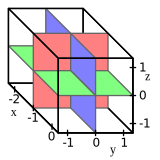
\includegraphics{1_c_echelon_plot_1}} 
\end{center}
%\caption{Part (a), Activity \ref{act:A1.2_7}.}
%\label{Fig:echelon_1}
\end{minipage} %\hspace{0.1in}
\begin{minipage}{1.5in}
\begin{center}
\resizebox{!}{1.5in}{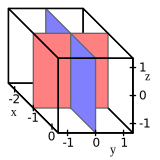
\includegraphics{1_c_echelon_plot_2}} 
\end{center}
%\caption{Part (b), Activity \ref{act:A1.2_7}.}
%\label{Fig:echelon_2}
\end{minipage} %\hspace{0.1in}
\begin{minipage}{1.5in}
\begin{center}
\resizebox{!}{1.5in}{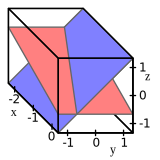
\includegraphics{1_c_echelon_plot_3}}
\end{center}
%\caption{Part (c), Activity \ref{act:A1.2_7}.}
%\label{Fig:echelon_3}
\end{minipage} 
\caption{Figures for Activity \ref{act:1_c_4}.}
\label{F:1_c_1}
\end{center}

\end{figure}

\begin{activity} \label{act:1_c_4} ~
\ba
\item For each part, the reduced row echelon form of the augmented matrix of a system of equations in variables $x$, $y$, and $z$ (in that order) is given. Use the reduced row echelon form to find the solution set to the original system of equations.
	\begin{enumerate}[i.]
	\begin{minipage}{1.4in}
	\item $\left[ \begin{array}{ccc|r} 1 & 0 & 0 & -1 \\ 0 & 1 & 0 & 3 \\ 0 & 0 & 0 & 0 \end{array} \right]$ %(the graph of this system is shown in Figure \ref{Fig:echelon_2})
	\end{minipage}
	\begin{minipage}{1.55in}
	\item $\left[ \begin{array}{ccr|r} 1 & 0 & 2 & -1 \\ 0 & 1 & -1 & 3 \\ 0 & 0 & 0 & 0 \end{array} \right]$ %(the graph of this system is shown in Figure \ref{Fig:echelon_3})
	\end{minipage}
	\begin{minipage}{1.4in}
	\item $\left[ \begin{array}{ccc|r} 1 & 0 & 0 & 2 \\ 0 & 1 & 0 & -1 \\ 0 & 0 & 1 & 3 \end{array} \right]$ %(the graph of this system is shown in Figure \ref{Fig:echelon_1})
	\end{minipage}

\item Each of the three systems above is represented as one of the graphs in Figure \ref{F:1_c_1}. Match each figure with a system.

	\end{enumerate}
	
\item The reduced row echelon form of the augmented matrix of a system of equations in variables $x$, $y$, $z$, and $t$ (in that order) is given. Use the reduced row echelon form to find the solution set to the original system of equations:  
\[\left[ \begin{array}{cccc|r} 1 & 3 & 0 & 0 & -1 \\ 0 & 0 & 1 & 2 & 4 \\ 0 & 0 & 0 & 0 & 1 \end{array} \right].\]



\ea

\end{activity}




\csection{Examples}

\ExampleIntro

\begin{example} Consider the linear system
\begin{align*}
2x_1 + 6x_3 &= x_2 + 2  \\
2x_3 - 4x_1  &=  2x_2\\
x_2 + 4x_3 - 2 &= 2x_1 + 6.
\end{align*}
	\ba
	\item Find the augmented matrix for this system.
	\item Use row operations to find a row echelon form of the augmented matrix of this system.
	\item Use row operations to find the reduced row echelon form of the augmented matrix of this system. 
	\item Find the solution(s), if any, to the system.
	\ea
	
\ExampleSolution Before we can find the augmented matrix of this system, we need to rewrite the system so that the variables are all on one side and the constant terms are on the other side of the equations. Doing so yields the equivalent system
\begin{alignat*}{4}
{2}x_1 	&{}-{}		&{}x_2		&{}+{}	&{6}x_3	&{}={}	& \ 2&{}   \\
{-4}x_1	&{}-{} 		&{2}x_2 		&{}+{}	&{2}x_3	 &{}={} 	& \ 0&{} \\
{-2}x_1	&{}+{}		&{}x_2		&{}+{} 	&{4}x_3	&{}={} 	& \ 8&{.}
\end{alignat*}
Note that this is not the only way to rearrange the system. For example, for the second equation, could be written instead as $4x_1+2x_2-2x_3=0$ to minimize the number of negative signs in the equation. 
\ba
\item The augmented matrix for this system is 
\[\left[ \begin{array}{rrc|c} 2&-1&6&2 \\ -4&-2&2&0 \\ -2&1&4&8 \end{array} \right].\]
\item Our first steps to row echelon form are to eliminate the entries below the leading entry in the first row. To do this we replace row two with row two plus 2 times row 1 and we replace row three with row three plus row one. This produces the row equivalent matrix
\[\left[ \begin{array}{crc|c} 2&-1&6&2 \\ 0&-4&14&4 \\ 0&0&10&10 \end{array} \right].\]
This matrix is now in row echelon form. 
\item To continue to find the reduced row echelon form, we replace row two with row two times $-\frac{1}{4}$ to get a leading 1 in the second row, and we replace row three with row three times $\frac{1}{10}$ to get a leading 1 in the third row and obtain the row equivalent matrix
\[\renewcommand{\arraystretch}{1.4} \left[ \begin{array}{crr|r} 2&-1&6&2 \\ 0&1&-\frac{7}{2}&-1 \\ 0&0&1&1 \end{array} \right].\]
Now we perform backwards elimination to make the entries above the leading $1$s equal to $0$, starting with the third column and working backwards. Replace row one with row one minus $6$ times row three and replace row two with row two plus $\frac{7}{2}$ row three to obtain the row equivalent matrix
\[\renewcommand{\arraystretch}{1.4} \left[ \begin{array}{crc|r} 2&-1&0&-4 \\ 0&1&0&\frac{5}{2} \\ 0&0&1&1 \end{array} \right].\] 
For the second column, we replace row one with row one plus row two to obtain the row equivalent matrix
\[\renewcommand{\arraystretch}{1.4} \left[ \begin{array}{ccc|r} 2&0&0&-\frac{3}{2} \\ 0&1&0&\frac{5}{2} \\ 0&0&1&1 \end{array} \right].\] 
Since the leading entry in row one is not a one, we have one more step before we have the reduced row echelon form. Finally, we replace row one with row one times $\frac{1}{2}$. This gives us the reduced row echelon form
\[\renewcommand{\arraystretch}{1.4} \left[ \begin{array}{ccc|r} 1&0&0&-\frac{3}{4} \\ 0&1&0&\frac{5}{2} \\ 0&0&1&1 \end{array} \right].\] 
\item We can read off the solution to the system from the reduced row echelon form: $x_1 = -\frac{3}{4}$, $x_2 = \frac{5}{2}$, and $x_3 = 1$. You should check in the original equations to make sure we have the correct solution. 
\ea

 \end{example}
 
 \begin{example} In this example, $a$ and $b$ are unknown scalars. Consider the system with augmented matrix 
 \[\left[ \begin{array}{ccc|c} 1&2&a&3 \\ 1&0&0&b \\ 0&1&1&0 \end{array} \right].\] 
 Find all values of $a$ and $b$ so that the system has:
 	\ba
	\item Exactly one solution (and find the solution)
	\item No solutions
	\item Infinitely many solutions (and find all solutions)
	\ea

\ExampleSolution Let $x_1$, $x_2$, and $x_3$ be the variables corresponding to the first, second, and third columns, respectively, of the augmented matrix. To answer these questions, we row reduce the augmented matrix. We interchange rows one and two and then also rows two and three to obtain the matrix
\[\left[ \begin{array}{ccc|c} 1&0&0&b  \\ 0&1&1&0 \\ 1&2&a&3  \end{array} \right].\] 
Now we replace row three with row three minus row one to produce the row equivalent matrix 
\[\left[ \begin{array}{crc|r} 1&0&0&b  \\ 0&1&1&0 \\ 0&2&a&3-b  \end{array} \right].\] 
Next, replace row three with row three minus $2$ times row two. This yields the row equivalent matrix
\[\left[ \begin{array}{ccc|c} 1&0&0&b  \\ 0&1&1&0 \\ 0&0&a-2&3-b  \end{array} \right].\] 
We now have a row echelon form. 
\ba
\item The system will have exactly one solution when the last row has the form $[0 \ 0 \ u \ v]$ where $u$ is not zero. Thus, the system has exactly one solution when $a-2 \neq 0$, or when $a \neq 2$.  In this case, the solution is 
\begin{align*}
x_3 &= \frac{3-b}{a-2}, \\
x_2 &= -x_3 = \frac{b-3}{a-2} \\
x_1 &= b.
\end{align*}
You should check to ensure that this solution is correct. The other cases occur when $a = 2$. 
\item When $a=2$ and $3-b \neq 0$ (or $b \neq 3$), then we have a row of the form $[0 \ 0 \ 0 \ t]$, where $t$ is not $0$. In these cases there are no solutions.
\item When $a=2$ and $b = 3$, then the last row is a row of all zeros. In this case, the system is consistent and $x_3$ is a free variable, so the system has infinitely many solutions. The solutions are 
\begin{align*}
x_1 &= b \\
x_2 &= -x_3 \\
x_3 &\text{ is free.}
\end{align*}
You should check to ensure that this solution is correct.
\ea

 \end{example}

\csection{Summary}

In this section we learned about the row echelon and reduced row echelon forms of a matrix and some of the things these forms tell us about solutions to systems of linear equations. 
\begin{itemize}
\item A matrix is in row echelon form if 
	\begin{enumerate}
    \item All nonzero rows are above any rows of all zeros.
    \item Each \textbf{pivot} (the first nonzero entry) of a row is in a column to the right of the pivot of the row above it.
    \end{enumerate}
\item Once an augmented matrix is in row echelon form, we can use back substitution to solve the corresponding linear system. 
\item To reduce a matrix to row echelon form we do the following: 
	\begin{itemize}
	\item Begin with the leftmost nonzero column (if there is one). This will be a pivot column. 
	\item Select a nonzero entry in this pivot column as a pivot. If necessary, interchange rows to move this entry to the first row (this entry will be a pivot).
	\item Use row operations to create zeros in all positions below the pivot.
	\item Cover (or ignore) the row containing the pivot position and cover all rows, if any, above it. Apply the preceding steps to the submatrix that remains. Repeat the process until there are no more nonzero rows to modify.
	\end{itemize}
\item A matrix is in reduced row echelon form if it is in row echelon form and 
	\begin{enumerate}
    \item[(3)] The pivot in each nonzero row is 1.
    \item[(4)] Each pivot is the only nonzero entry in its column.
	\end{enumerate}
\item To obtain the reduced row echelon form from the row echelon form, beginning with the rightmost pivot and working upward and to the left, create zeros above each pivot. If a pivot is not 1, make it 1 by an appropriate row multiplication.
\item Both row echelon forms of an augmented matrix tell us about the number of solutions to the corresponding linear system.
	\begin{itemize}
	\item A linear system is inconsistent if and only if a row echelon form of the augmented matrix of the system contains a row of the form
    \[[0 \ 0 \ 0 \ \cdots \ 0 \ *],\]
    where $*$ is not zero. Another way to say this is that a linear system is inconsistent if and only if the last column of the augmented matrix of the system is a pivot column.
	\item A consistent linear system will have a unique solution if and only if each column but the last in the augmented matrix of the system is a pivot column. This is equivalent to saying that a consistent linear system will have a unique solution if and only if the consistent system has no free variables.
	\item A consistent linear system will have infinitely many solutions if and only if the coefficient matrix of the system contains a non-pivot column. In that case, the free variables corresponding to the non-pivot columns can be chosen arbitrarily and the basic variables corresponding to pivot columns can be written in terms of the free variables.
	\item A linear system can have no solutions, exactly one solution, or infinitely many solutions.
	\end{itemize}  
\end{itemize}




\csection{Exercises}
\be
\item Represent the following linear system in variables $x_1, x_2, x_3$ in augmented matrix form and use row reduction to find the general solution of the system.
\begin{alignat*}{5}
{}x_1 	&{}+{}	&{}x_2	&{}-{}	&{}x_3 	&= &{}4&{} \\
{}x_1	&{}+{}	&{2}x_2 &{}+{}	&{2}x_3 &= &{}3&{}\\
{2}x_1	&{}+{}	&{3}x_2 &{}-{}	&{3}x_3 &= &{}11&{.}
\end{alignat*}

\item Represent the following linear system in variables $x_1, x_2, x_3$ in augmented matrix form after rearranging the terms and use row reduction to find all solutions to the system. %change numbers to make it nicer. x1=19, x2=3, x3=10 currently
\begin{align*}
x_1 - x_3 - 2x_2 &= 3 \\
2x_3 + 2 &= x_1 +x_2\\
4x_2 + 2x_1 - 2 &= 5x_3.
\end{align*}

\item Check that the reduced row echelon form of the matrix 
\[ \left[ \begin{array}{rrrr} 1 &-1& 3& 2 \\ -1& 2&-4&-1 \\ 2&0&6&8 \end{array} \right] \]
is
\[ \left[ \begin{array}{cccc} 1 &0&0&1 \\ 0&1&0&2 \\ 0&0&1&1 \end{array} \right] \, .\]

\item Consider the following system:
\begin{alignat*}{5}
{}x 	&{}-{} 	&{2}y 	&{}+{} 	&{}z 		&{}={}	&\ {-}&1&{}   \\
{}		&{}		&{2}y	&{}-{} 	&{4}z	&{}={} 	& \ {}&6&{} \\ 
{}		&{}		&{h}y	&{}-{} 	&{2}z	&{}={} 	& \ {}&1&{.} 
\end{alignat*}
	\ba
	\item Find a row echelon form of the augmented matrix for this system.

	\item For which values of $h$, if any, does the system have (i.) no solutions, (ii.) exactly one solution, (iii.) infinitely many solutions? Find the solutions in each case.

	\ea

\item Find the general solution of the linear system corresponding to the following augmented matrix:
\[\left[ \begin{array}{rrcr|r} 1&-1&2&1&2 \\ -1&2&2&-1&-5\\ 1&1&10&2&-1 \end{array}  \right].\]

\item What are the conditions, if any, on the $a, b, c$ values so that the following augmented matrix corresponds to a consistent linear system? How many solutions will the consistent system have? Explain. 
\[\left[ \begin{array}{rrr|c} 1 & 2 & 3 &a \\ 2&3&7&b \\ -1&-4&-1&c \end{array}  \right].\]

\item In this exercise the symbol $\blacksquare$ denotes a non-zero number and the symbol * denotes any real number (including $0$).
\ba
\item Is the augmented matrix 
\[\left[ \begin{array}{cc|c} \blacksquare&*&* \\ 0&\blacksquare&* \end{array} \right]\]
in a form to which back substitution will easily give the solutions to the system?  Explain your reasoning. (Hint: In order to help see what happens in the general case, substitute some numbers in place of the $\blacksquare$'s and *'s and answer the question for that specific system first. Then determine if your answer generalizes.)


\item  The above matrix is a possible form of an augmented matrix with 2 rows and 3 columns corresponding to a linear system after forward elimination, i.e., a linear system for which back substitution will easily give the solutions. Determine the other possible such forms of the nonzero augmented matrices with 2 rows and 3 columns. As in part (a), use the symbol $\blacksquare$ to denote a non-zero number and * to denote any real number.


\ea


\item Give an example of a linear system with a unique solution for which a row echelon form of the augmented matrix of the system has a row of 0's.

\item Come up with an example of an augmented matrix with 0's in the rightmost column corresponding to an inconsistent system, if possible. If not, explain why not.

\item Find two different row echelon forms which are equivalent to the same matrix not given in row echelon form.


\item Determine all possible row echelon forms of a $2\times 2$ matrix. Use the symbol $\blacksquare$ to denote a non-zero number and * to denote a real number with no condition on being 0 or not to represent entries.

\item Label each of the following statements as True or False. Provide justification for your response.
	\ba
	\item \textbf{True/False} The number of pivots of an $m \times n$ matrix cannot exceed $m$. (Note: Here $m$, $n$ are some unknown numbers.)
	\item \textbf{True/False} The row echelon form of a matrix is unique.
	\item \textbf{True/False} The reduced row echelon form of a matrix is unique.
	\item \textbf{True/False} A system of equations where there are fewer equations than the number of unknowns (known as an underdetermined system) cannot have a unique solution.
	\item \textbf{True/False} A system of equations where there are more equations than the number of unknowns (known as an overdetermined system) cannot have a unique solution.
	\item  \textbf{True/False} If a row echelon form of the {\em augmented matrix} of a system of three equations in two unknowns has three pivots, then the system is inconsistent.
	\item \textbf{True/False} If the coefficient matrix of a system has pivots in every row, then the system is consistent.
	\item \textbf{True/False} If there is a row of zeros in a row echelon form of the augmented matrix of a system of equations, the
system has infinitely many solutions.
	\item \textbf{True/False} If there is a row of zeros in a row echelon form of the augmented matrix of a system of $n$ equations in $n$ variables, the system has infinitely many solutions.
	\item \textbf{True/False} If a linear system has no free variables, then the system has a unique solution.
	\item  \textbf{True/False} If a linear system has a free variable, then the system has infinitely many solutions.
	\ea
\ee


\csection{Project: Modeling a Chemical Reaction}

Recall the chemical equation
\begin{equation*}
\text{C}_2\text{H}_6 + \text{O}_2 \to \text{CO}_2 + \text{H}_2\text{O} %\label{eq:reaction1}
\end{equation*}
from the beginning of this section. This equation illustrates the reaction between ethane ($\text{C}_2\text{H}_6$) and oxygen ($\text{O}_2$),called the \emph{reactants}, to produce carbon dioxide ($\text{CO}_2$) and water ($\text{H}_2\text{O}$), called the \emph{products} of the reaction.  In any chemical reaction, the total mass of the reactants must equal the total mass of the products. In our reaction the chemicals involved are made up of carbon (C), hydrogen (H), and oxygen (O) atoms. To balance the equation, we need to know how many molecules of each chemical are combined to preserve the number of atoms of C, H, and O.

Let $x_1$ be the number of molecules of $\text{C}_2\text{H}_6$, $x_2$ the number of molecules of $\text{O}_2$, $x_3$ the number of molecules of $\text{CO}_2$, and $x_4$ the number of molecules of $\text{H}_2\text{O}$ in the reaction. We can then represent this reaction as
\[x_1 \text{C}_2\text{H}_6 + x_2 \text{O}_2 \to x_3 \text{CO}_2 + x_4 \text{H}_2\text{O}.\]

In each molecule (e.g., ethane $\text{C}_2\text{H}_6$), the subscripts indicate the number of atoms of each element in the molecule. So 1 molecule of ethane contains 2 atoms of carbon and 6 atoms of hydrogen. Thus, there are 2 atoms of carbon in $\text{C}_2\text{H}_6$ and 0 atoms of carbon in $\text{O}_2$, giving us  $2x_1$ carbon atoms in $x_1$ molecules of $\text{C}_2\text{H}_6$ and 0 carbon atoms in $x_2$ molecules of $\text{O}_2$. On the product side of the reaction there is 1 carbon atom in $\text{CO}_2$ and 0 carbon atoms in $\text{H}_2\text{O} $. To balance the reaction, we know that the number of carbon atoms in the products must equal the number of carbon atoms in the reactants. 

\begin{pactivity} \label{act:1_c_reaction_1} ~
	\ba
	\item Set up an equation that balances the number of carbon atoms on both sides of the reaction.

	\item Balance the numbers of hydrogen and oxygen atoms in the reaction to explain why
\begin{align*}
6x_1 &= 2x_4 \\
2x_2 &= 2x_3 + x_4.
\end{align*}

	\item So the system of linear equations that models this chemical reaction is  \begin{alignat*}{5}
{2}x_1 	&{}		&{}		&{}-{}	&{}x_3	&{}		&{} 			&{}={}	& \ 0&{}   \\
{6}x_1	&{} 		&{} 		&{}		&{}		&{}-{}	&{2}x_4 	&{}={} 	& \ 0&{} \\
{}			&{}		&{2}x_2	&{}-{} 	&{2}x_3	&{}-{}	&{}x_4		&{}={} 	& \ 0&{.}
\end{alignat*}

Find all solutions to this system and then balance the reaction. Note that we cannot have a fraction of a molecule in our reaction.  (Hint: Some of the work needed is done in Preview Activity \ref{pa:1_c}.) 
	\ea

\end{pactivity}

\begin{pactivity} Chemical reactions can be very interesting. 
\ba
\item Carbon dioxide, $\text{CO}_2$, is a familiar product of combustion. For example, when we burn glucose, $\text{C}_6\text{H}_{12}\text{O}_6$, the products of the reaction are carbon dioxide and water:
\begin{equation}
\text{C}_6\text{H}_{12}\text{O}_6 + \text{O}_2 \to \text{CO}_2 + \text{H}_2\text{O}.\label{eq:reaction2}
\end{equation}
Use the techniques developed in this project to balance this reaction.

\item To burn glucose, we need to add oxygen to make the combustion happen. Carbon dioxide is different in that it can burn without the presence of oxygen. For example, when we mix magnesium (Mg) with dry ice ($\text{CO}_2$), the products are magnesium oxide (MgO) and carbon (C). This is an interesting reaction to watch: you can see it at many websites, e.g.,
\url{http://www.ebaumsworld.com/video/watch/404311/} or 
\url{https://www.youtube.com/watch?v=-6dfi8LyRLA}.

Use the method determined above to balance the chemical reaction 
\begin{equation}
\text{Mg} + \text{CO}_2 \to \text{MgO} + \text{C}. \label{eq:reaction3}
\end{equation}

\ea

\end{pactivity}



 %3
\input{1_d_vector_representation_F20.tex} %4
\achapter{5}{The Matrix-Vector Form of a Linear System} \label{chap:matrix_vector}

\vspace*{-17 pt}
\framebox{
\parbox{\dimexpr\linewidth-3\fboxsep-3\fboxrule}
{\begin{fqs}
\item How and when is the matrix-vector product $A \vx$ defined? 
\item How can a system of linear equations be written in matrix-vector form? 
\item How can we tell if the system $A \vx = \vb$ is consistent for a given vector $\vb$?
\item How can we tell if the system $A \vx = \vb$ is consistent for every vector $\vb$?
\item What is a homogeneous system? What can we say about the solution set to a homogeneous system? 
\item What must be true about pivots in the coefficient matrix $A$ in order for the homogeneous system $A \vx = \vzero$ to have a unique solution? 
\item How are the solutions to the nonhomogeneous system $A \vx = \vb$ related to the solutions of the corresponding homogeneous system $A \vx = \vzero$?
\end{fqs}}}% \hspace*{3 pt}}

\vspace*{13 pt}

\csection{Application: Modeling an Economy}
\label{sec:appl_model_econ}

An economy is a very complex system. An economy is not a well-defined object, there are many factors that influence an economy, and it is often unclear how the factors influence each other. Mathematical modeling plays an important role in attempting to understand an economy.

In 1941 Wassily Leontief developed the first empirical model of a national economy. Around 1949 Leontief used data from the U.S. Bureau of Labor Statistics to divide the U.S. economy into 500 sectors. He then set up linear equations for each sector. This system was too large for the computers at the time to solve, so he then aggregated the information into 42 sectors. The Harvard Mark II computer was used to solve this system, one of the first significant uses of computers for mathematical modeling. Leontief won the 1973 Nobel Prize in economics for his work. 

With such large models (Leontief's models are called \emph{input-output} models) it is important to find a shorthand way to represent the resulting systems.  In this section we will see how to represent any size system of linear equations in a very convenient way. Later, we will analyze a small economy using input-output models. 

\csection{Introduction}
\label{sec:mv_form_intro}

There is another useful way to represent a system of linear equations using a matrix-vector product that we investigate in this section. To understand how this product comes about, recall that we can represent the linear system 
\begin{alignat*}{5}
x_1 		&{}+{} 	&{4}x_2 	&{}+{}	&{2}x_3 	&{}+{}	&{4}x_4	&{}={}	&1 \\
{2}x_1 	&{}-{} 	&{}x_2 		&{}-{}	&{5}x_3 	&{}-{}	&{}x_4	&{}={}	&2 \\
{3}x_1 	&{}+{} 	&{7}x_2 	&{}+{}	&{}x_3 		&{}+{}	&{7}x_4	&{}={}	&3 \\
\end{alignat*}
as a vector equation as
\begin{equation} \label{eq:PA1e_1}
x_1\left[ \begin{array}{c} 1\\2\\3 \end{array} \right] + x_2\left[ \begin{array}{r} 4\\-1\\7 \end{array} \right] + x_3\left[ \begin{array}{r} 2\\-5\\1 \end{array} \right] + x_4\left[ \begin{array}{r} 4\\-1\\7 \end{array} \right]= \left[ \begin{array}{c} 1\\2\\3 \end{array} \right].
\end{equation}
We can view the left hand side of Equation ( \ref{eq:PA1e_1}) as a \textbf{matrix-vector product}. Specifically, if $A = \left[ \begin{array}{crrr} 1&4&2&4 \\ 2&-1&-5&-1 \\ 3&7&1&7 \end{array} \right]$ and $\vx = \left[ \begin{array}{c} x_1 \\x_2 \\x_3 \\x_4 \end{array} \right]$, then we define the \emph{matrix-vector product} $A\vx$ as the left hand side Equation \eqref{eq:PA1e_1}. So the matrix-vector product $A\vx$ is the linear combination of the columns of $A$ with weights from the vector $\vx$ in order. 

With this definition, the vector equation in \eqref{eq:PA1e_1} can be expressed as a matrix-vector equation as
\[\left[ \begin{array}{crrr} 1&4&2&4 \\ 2&-1&-5&-1 \\ 3&7&1&7 \end{array} \right] \left[ \begin{array}{c} x_1 \\x_2 \\x_3\\x_4 \end{array} \right] = \left[ \begin{array}{c} 1\\2\\3 \end{array} \right] \,.\]
We call this representation the \textbf{matrix-vector form} of the system. Note that the matrix $A$ in this expression is the same as the coefficient matrix that appears in the augmented matrix representation of the system.

We can use the above definition of the matrix-vector product as a linear combination with any matrix and any vector, as long as it is meaningful to use the entries in the vector as weights for the columns of the matrix. For example, for $A=\left[ \begin{array}{cc} 1&2\\3&1\\1&1 \end{array} \right]$ and $\vv = \left[ \begin{array}{c} 3\\4 \end{array} \right]$, then we can define $A\vv$ to be the linear combination of the columns of $A$ with weights 3 and 4:
\[A\vv= 3 \left[ \begin{array}{c} 1\\3\\1 \end{array} \right] + 4 \left[ \begin{array}{c} 2\\1\\1 \end{array} \right] = \left[ \begin{array}{c} 11\\13\\7 \end{array} \right] \, .\]
However, note that if $\vv$ had three entries, this definition would not make sense since we do not have three columns in $A$. In those cases, we say $A\vv$ is not defined. We will later see that this definition can be generalized to matrix-matrix products, by treating the vector as a special case of a matrix with one column.

\begin{pa} \label{pa:1_e} ~
\be

\item Write the vector equation
\[x_1 \left[ \begin{array}{c} 1 \\ 1 \\ 2 \end{array} \right] +x_2 \left[ \begin{array}{c}  1\\ 2\\ 3 \end{array} \right] + x_3 \left[ \begin{array}{r} -1 \\ 2 \\ -3 \end{array} \right] = \left[ \begin{array}{c} 4 \\ 3\\ 11 \end{array} \right] \]
in matrix-vector form. Note that this is the vector equation whose augmented matrix representation was given in Problem 2 in Preview Activity \ref{pa:1_b}. Compare your matrix $A$ and the right hand side vector to the augmented matrix. Do not solve the system.

\item Given the matrix-vector equation
\[ \left[ \begin{array}{crr} 1 & 2 & -1 \\ 0&1&2\\1&-2&-3 \end{array} \right] \vx = \left[\begin{array}{r} -3\\3\\-7 \end{array}\right] \]
represent the system corresponding to this equation. Note that this should correspond to the system (or an equivalent system where an equation might be multiplied by $(-1)$) in Problem 1 of Preview Activity \ref{pa:1_b}.


\item Find the indicated matrix-vector products, if possible. Express as one vector.
    \ba
    \item $\left[ \begin{array}{cr} 2& -2 \\ 1& 2 \end{array} \right] \left[ \begin{array}{r} 1 \\ -1 \end{array} \right]$

    

    \item $\left[ \begin{array}{rrr} 1 & 0 & 2\\ 2 & -2 & 3  \end{array} \right] \left[ \begin{array}{r} 2\\1 \end{array} \right]$

    
		
		\item $\left[ \begin{array}{rrc} -6 & -2 & 1\\ 2 & -2 & 1  \end{array} \right] \left[ \begin{array}{r} 1\\-3 \\1\end{array} \right]$

    

    \ea

\item As you might have noticed, systems with all the constants being 0 are special in that they always have a solution. (Why?) So we might consider grouping systems into two types: Those of the form $A \vx = \vb$, where not all of the entries of the vector $\vb$ are $0$, and those of the form $A \vx = \vzero$, where $\vzero$ is the vector of all zeros. Systems like $A \vx = \vb$, where $\vb$ contains at least one non-zero entry, are called \emph{nonhomogeneous}\index{nonhomogeneous system}  systems, and systems of the form $A \vx = \vzero$ are called \emph{homogeneous}\index{homogeneous system} systems. For every nonhomogeneous system $A \vx = \vb$ there is a corresponding homogeneous system $A \vx = \vzero$, and there is a useful connection between the solutions to the nonhomogeneous system and the corresponding homogeneous system. For example, consider the nonhomogeneous system
\[A \vx = \vb\]
with 
 \begin{equation} \label{eq:PA1e_2} 
A = \left[ \begin{array}{ccc} 1 & 1 & 2  \\ 1 & 2 & 1  \end{array} \right], \ \vx = \left[ \begin{array}{c} x_1 \\ x_2 \\ x_3 \end{array} \right], \ \text{ and } \ \vb =  \left[ \begin{array}{r} 0 \\ -2 \end{array} \right].
\end{equation}
The augmented matrix representation of this system is $[A \ | \ \vb]$. If we reduce this augmented matrix, we find 
\[\left[ \begin{array}{ccr|r} 1 & 0 & 3 & 2 \\ 0 & 1 & -1 & -2 \end{array} \right].\]
From this RREF, we immediately see that the general solution is that $x_3$ is free, $x_2 = x_3-2$, and $x_1 = 2-3x_3$. In vector form, we can represent this general solution as
\begin{equation} \label{eq:PA1e_3}
\left[ \begin{array}{c} x_1 \\ x_2 \\ x_3 \end{array} \right] = \left[ \begin{array}{c} 2-3x_3 \\ x_3-2 \\ x_3 \end{array} \right] = \left[ \begin{array}{r} 2 \\ -2 \\ 0 \end{array} \right] + x_3\left[ \begin{array}{r} -3 \\ 1 \\ 1 \end{array} \right].
\end{equation}
The rightmost expression above is called the \emph{parametric vector form}\index{parametric vector form} of the solution. 

If we had a system where the general solution involved more than one free variable, then we would write the parametric vector form to include one vector multiplying each free variable. For example, if the general solution of a system were that $x_2$ and $x_3$ are free and $x_1=2+x_2+3x_3$, then the parametric vector form would be 
\[ \vx = \left[ \begin{array}{c} 2+ x_2+3x_3 \\ x_2 \\ x_3 \end{array} \right] = \left[ \begin{array}{c} 2 \\ 0 \\ 0 \end{array} \right] + x_2 \left[ \begin{array}{c} 1 \\ 1 \\ 0 \end{array} \right] + x_3 \left[ \begin{array}{c} 3 \\ 0 \\ 1\end{array} \right] \, . \]

Note that the parametric vector form expresses the solutions as a linear combination of a number of vectors, depending on the number of free variables, with an added constant vector. This expression helps us in interpreting the solution set geometrically, as we will see in this section.


	
	\ba
	\item Find the general solution to the homogeneous system 
	\[A \vx = \vzero\]
	with $A$ and $\vx$ as in (\ref{eq:PA1e_2}) and compare it to the solution to the nonhomogeneous system in (\ref{eq:PA1e_3}). What do you notice? 


	\item Find the general solution to the nonhomogeneous system 
	\[A \vx = \vb\]
	with 
\[A = \left[ \begin{array}{ccr} 1&2&-1 \\ 2&4&-2 \end{array} \right], \ \vx =  \left[ \begin{array}{c} x_1 \\ x_2 \\ x_3 \end{array} \right], \ \text{ and } \ \vb =  \left[ \begin{array}{r} -1 \\ 1 \end{array} \right].\]
and express it in parametric vector form. Then find the general solution to the corresponding homogeneous system and express it in parametric vector form. How are the two solution sets related? 


	\item Make a conjecture about the relationship between the solutions to a consistent nonhomogeneous system $A \vx = \vb$ and the corresponding homogeneous system $A \vx = \vzero$. Be as specific as possible.

	
	\ea

\ee

\end{pa} 



\csection{The Matrix-Vector Product}
\label{sec:mv_prod}

The matrix-vector product we defined in Preview Activity \ref{pa:1_e} for a specific example generalizes in a very straightforward manner, and provides a convenient way to represent a system of linear equations of any size using matrices and vectors. In addition to providing us with an algebraic approach to solving systems via matrices and vectors -- leading to a powerful geometric relationship between solution sets of homogeneous and non-homogeneous systems -- this representation allows us to think of a linear system from a dynamic perspective, as we will see later in the section on matrix transformations. 

The matrix-vector product $A \vx$ is a linear combination of the columns of $A$ with weights from $\vx$. To define this product in general, we will need a little notation. Recall that a matrix is made of rows and columns -- the entries reading from left to right form the \emph{rows}\index{matrix!rows} of the matrix and the entries reading from top to bottom form the \emph{columns}\index{matrix!columns}. For example, the matrix  
\[A = \left[ \begin{array}{cccc} 1 & 2 & 3 & 4 \\ 5 & 6 & 7 & 8  \\ 9 & 10 & 11 & 12 \end{array} \right].\]
has three rows and four columns. The number of rows and columns of a matrix is called the \emph{size}\index{matrix!size} of the matrix, so $A$ is a 3 by 4 matrix (also written as $3 \times 4$). We often need to have a way to reference the individual entries of a matrix $A$, and to do so we typically give a label, say $a_{ij}$ to the entry in the $i$th row and $j$th column of $A$. So in our example we have $a_{23}=7$. We also write $A = [a_{ij}]$ to indicate a matrix whose $i,j$th entry is $a_{ij}$. At times it is convenient to write a matrix in terms of its rows or columns. If $A = [a_{ij}]$ is an $m \times n$ matrix, then we will write
\[A = \left[ \begin{array}{ccccc}
a_{11} & a_{12}  & \cdots    & a_{1n-1} & a_{1n} \\
a_{21} & a_{22}  & \cdots    & a_{2n-1} & a_{2n} \\
 \vdots &         & \ddots    &     &\vdots \\
a_{m1} & a_{m2}  & \cdots    & a_{mn-1} & a_{mn}
\end{array} \right]\]
or, if we let $\vr_1, \vr_2, \ldots, \vr_m$ denote the rows of the matrix $A$, then we can write $A$ as\footnote{Technically, the rows of $A$ are made from the entries of the row vectors, but we use this notation as a shorthand.}
\[A = \left[ \begin{array}{c} \vr_1 \\ \vr_2 \\ \vdots \\ \vr_m \end{array} \right].\]
We can also write $A$ in terms of its columns, $\vc_1, \vc_2, \ldots, \vc_n$, as
\[A = [\vc_1 \ \vc_2 \ \cdots \ \vc_n].\]

In general, the product of a matrix with a vector is defined as follows. 



\begin{definition} Let $A$ be an $m \times n$ matrix with columns $\vc_1$, $\vc_2$, $\ldots$, $\vc_n$, and let $\vx = \left[ \begin{array}{c} x_1 \\ x_2 \\ \vdots \\ x_n \end{array} \right]$ be a vector in $\R^n$. The \textbf{matrix-vector product}\index{matrix-vector product} $A\vx$ is
\[A \vx = x_1 \vc_1 + x_2 \vc_2 + \cdots + x_n \vc_n.\]
\end{definition}



\noindent \textbf{Important Note:} The matrix-vector product $A \vx$ is defined only when the number of entries of the vector $\vx$ is equal to the number of columns of the matrix $A$. That is, if $A$ is an $m \times n$ matrix, then $A\vx$ is defined only if $\vx$ is a column vector with $n$ entries. 


\csection{The Matrix-Vector Form of a Linear System}
\label{sec:mv_form}

As we saw in Preview Activity \ref{pa:1_e}, the matrix-vector product provides us with a short hand way of representing a system of linear equations. In general, every linear system can be written in matrix-vector form as follows.

The linear system
\begin{alignat*}{5}
{a_{11}}x_1 	&{}+{} 	&{a_{12}}x_2 	&{}+{}	&\cdots 			&{}+{}	&{a_{1n}}x_n		&{}={}	&b_1 \\
{a_{21}}x_1 	&{}+{} 	&{a_{22}}x_2		&{}+{}	&\cdots			&{}+{}	&{a_{2n}}x_n		&{}={}	&b_2 \\
{} 				&{} 		&{}					&{}		&\vdots \ \		&{}		&{}					&{}		&{} \\
{a_{m1}}x_1 	&{}+{} 	&{a_{2m}}x_2	&{}+{}	&\cdots			&{}+{}	&{a_{mn}}x_n	&{}={}	&b_m 
\end{alignat*} 
of $m$ equations in $n$ unknowns can be written in matrix-vector form as $A\vx = \vb$, where 
\[A = \left[ \begin{array}{cccc}
a_{11} & a_{12} & \cdots & a_{1n} \\
a_{21} & a_{22} & \cdots & a_{2n} \\
\vdots &        & \ddots    & \vdots \\
a_{m1} & a_{m2} & \cdots & a_{mn}
\end{array} \right],  \ \ \ \vx = \left[ \begin{array}{c} x_1 \\ x_2 \\ \vdots \\ x_n \end{array} \right],  \ \ \ \text{ and } \ \ \ \vb = \left[ \begin{array}{c} b_1 \\ b_2 \\ \vdots \\ b_m \end{array} \right].\]
This general system can also be written in the vector form
\[x_1  \left[ \begin{array}{c} a_{11}  \\ a_{21} \\ \vdots \\ a_{m1} \end{array} \right] + x_2 \left[ \begin{array}{c} a_{12}  \\ a_{22} \\ \vdots \\ a_{m2} \end{array} \right]  + \cdots + x_n \left[ \begin{array}{c} a_{1n}  \\ a_{2n}  \\ \vdots \\ a_{mn} \end{array} \right] = \left[ \begin{array}{c} b_1 \\ b_2 \\ \vdots \\ b_m \end{array} \right].\]



With this last representation, we now have four different ways to represent a system of linear equations (as a system of linear equations, as an augmented matrix, in vector equation form, and in matrix-vector equation form), and it is important to be able to translate between them. As an example, the system
\begin{alignat*}{5}
x_1 		&{}+{} 	&{4}x_2 	&{}+{}	&{2}x_3 	&{}+{}	&{4}x_4	&{}={}	&1 \\
{2}x_1 	&{}-{} 	&{}x_2 		&{}-{}	&{5}x_3 	&{}-{}	&{}x_4	&{}={}	&2 \\
{3}x_1 	&{}+{} 	&{7}x_2 	&{}+{}	&{}x_3 		&{}+{}	&{7}x_4	&{}={}	&3 \\
\end{alignat*}
from the introduction to this section has corresponding augmented matrix
\[\left[ \begin{array}{crrr|c} 1&4&2&4&1 \\ 2&-1&-5&-1&2 \\ 3&7&1&7&3 \end{array} \right],\]
is expressed in vector form as 
\[x_1\left[ \begin{array}{c} 1\\2\\3 \end{array} \right] + x_2\left[ \begin{array}{r} 4\\-1\\7 \end{array} \right] + x_3\left[ \begin{array}{r} 2\\-5\\1 \end{array} \right] + x_4\left[ \begin{array}{r} 4\\-1\\7 \end{array} \right]= \left[ \begin{array}{c} 1\\2\\3 \end{array} \right],\]
and has matrix-vector form
\[\left[ \begin{array}{crrr} 1&4&2&4 \\ 2&-1&-5&-1 \\ 3&7&1&7 \end{array} \right] \left[ \begin{array}{c} x_1 \\x_2 \\ x_3 \\ x_4 \end{array} \right] = \left[ \begin{array}{c} 1 \\ 2 \\ 3 \end{array} \right].\]


\begin{activity} In this activity, we will use the equivalence of the different representations of a system to make useful observations about when a system represented as $A\vx=\vb$ has a solution. 

\ba
\item Consider the system
\[\left[ \begin{array}{ccr} 1&2&-1 \\ 2&1&3 \end{array} \right] \left[ \begin{array}{c} x_1 \\ x_2 \\ x_3\end{array} \right] = \left[ \begin{array}{c} 2 \\ 6 \end{array} \right].\]
Write the matrix-vector product on the left side of this equation as a linear combination of the columns of the coefficient matrix. Find weights that make the vector $\left[ \begin{array}{c} 2 \\ 6 \end{array} \right]$ a linear combination of the columns of the coefficient matrix. 

\item From this point on we consider the general case where $A$ is an $m \times n$ matrix. Use the vector equation representation to explain why the system $A \vx = \vb$ has a solution if and only if $\vb$ is a linear combination of the columns of $A$. (Note that `if and only if' is an expression to mean that if one side of the expression is true, then the other side must also be true.) (Hint: Compare to what you did in part (a).)



\item Use part (b) and the definition of span to explain why the system $A \vx = \vb$ has a solution if and only if the vector $\vb$ is in the span of the columns of $A$. 



\item Use part (c) to explain why the system $A \vx = \vb$ always has a solution for any vector $\vb$ in $\R^m$ if and only if the span of the columns of $A$ is all of $\R^m$.



\item Use the augmented matrix representation and the criterion for a consistent system to explain why the system $A \vx = \vb$ is consistent for all vectors $\vb$ if and only if $A$ has a pivot position in every row.



\ea

\end{activity}

We summarize our observations from the above activity in the following theorem.

\begin{theorem} Let $A$ be an $m \times n$ matrix. The following statements are equivalent:
    \begin{enumerate}
    \item The matrix equation $A \vx = \vb$ has a solution for every vector $\vb$ in $\R^m$.
    \item Every vector $\vb$ in $\R^m$ can be written as a linear combination of the columns of $A$.
    \item The span of the columns of $A$ is $\R^m$.
    \item The matrix $A$ has a pivot position in each row.
    \end{enumerate}
\end{theorem}



In the future, if we need to determine whether a system has a solution for every $\vb$, we can refer to this theorem without having to argue our reasoning from scratch.



\subsection*{Properties of the Matrix-Vector Product}

As we have done before, we have a new operation (the matrix-vector product), so we should wonder what properties it has. 


\begin{activity} \label{act:A1.4_8} In this activity, we consider whether the matrix-vector product distributes vector addition. In other words: Is $A(\vu + \vv)$ equal to $A\vu + A\vv$?\\

We work with arbitrary vectors $\vu, \vv$ in $\R^3$ and an arbitrary matrix $A$ with 3 columns (so that $A\vu$ and $A\vv$ are defined) to simplify notation. Let $A = [\vc_1 \ \vc_2 \ \vc_3]$ (note that each $\vc_i$ represents a column of $A$), $\vu = \left[ \begin{array}{c} u_1 \\ u_2 \\ u_3 \end{array} \right]$, and $\vv = \left[ \begin{array}{c} v_1 \\ v_2 \\ v_3 \end{array} \right]$. Use the definition of the matrix-vector product along with the properties of vector operations to show that
\[A(\vu + \vv)= A\vu + A\vv.\]


\end{activity}



Similar arguments using the definition of matrix-vector product along with the properties of vector operations can be used to show the following theorem:


\begin{theorem} \label{thm:IMT_1_e} Let $A$ be an $m \times n$ matrix, $\vu$ and $\vv$ $n \times 1$ vectors, and $c$ a scalar. Then
\begin{enumerate}
\item $A(\vu + \vv) = A\vu + A\vv$
\item $c(A\vv) = A(c\vv)$
\end{enumerate}
\end{theorem}

\csection{Homogeneous and Nonhomogeneous Systems}
\label{sec:homog_sys}

As we saw before, the systems with all the right hand side constants being 0 are special in that they always have a solution. (Why?) So we might consider grouping systems into two types: Those of the form $A \vx = \vb$, where not all of the entries of the vector $\vb$ are $0$, and those of the form $A \vx = \vzero$, where $\vzero$ is the vector of all zeros. Systems like $A \vx = \vb$, where $\vb$ contains at least one non-zero entry, are called \textbf{nonhomogeneous} systems, and systems of the form $A \vx = \vzero$ are called \textbf{homogeneous} systems. For every nonhomogeneous system $A \vx = \vb$ there is a corresponding homogeneous system $A \vx = \vzero$. We now investigate the connection between the solutions to the nonhomogeneous system and the corresponding homogeneous system. 

\vspace{0.2cm}

\begin{activity} In this activity we will consider the relationship between the solution sets of nonhomogeneous systems and those of the corresponding homogeneous systems.

\ba 
\item Find the solution sets of the system
\[A \vx = \vb\]
where 
\[ A = \left[ \begin{array}{ccc} 1 & 1 & 2  \\ 1 & 2 & 1  \end{array} \right], \ \vx = \left[ \begin{array}{c} x_1 \\ x_2 \\ x_3 \end{array} \right], \ \text{ and } \ \vb =  \left[ \begin{array}{r} 0 \\ -2 \end{array} \right] \]
and the corresponding homogeneous system (i.e. where we replace $\vb$ with $\vzero$.)


\item Find the solution sets of the system
\[A \vx = \vb\]
where 
\[A = \left[ \begin{array}{ccr} 1&2&-1 \\ 2&4&-2 \end{array} \right], \ \vx =  \left[ \begin{array}{c} x_1 \\ x_2 \\ x_3 \end{array} \right], \ \text{ and } \ \vb =  \left[ \begin{array}{r} -1 \\ 1 \end{array} \right]\]
and the corresponding homogeneous system.


\item What are the similarities/differences between solutions of the nonhomogeneous system and its homogeneous counterpart?


\ea
\end{activity}


As we saw in the above activity, there is a relationship between solutions of a nonhomogeneous and the corresponding homogeneous system. Let us formalize this relationship. If the general solution of a system involves free variables, we can represent the solutions in \textbf{parametric vector form} to have a better idea about the geometric representation of the solution set. Suppose the solution is that $x_3$ is free, $x_2 = -2+x_3$, and $x_1 = 2-3x_3$. In vector form, we can represent this general solution as
\begin{equation} 
\left[ \begin{array}{c} x_1 \\ x_2 \\ x_3 \end{array} \right] = \left[ \begin{array}{c} 2-3x_3 \\ x_3-2 \\ x_3 \end{array} \right] = \left[ \begin{array}{r} 2 \\ -2 \\ 0 \end{array} \right] + x_3\left[ \begin{array}{r} -3 \\ 1 \\ 1 \end{array} \right].
\end{equation}
From this representation, we see that the solution set is a line through the origin (formed by multiples of $\left[ \begin{array}{r} -3 \\ 1 \\ 1 \end{array} \right]$) shifted by the added vector $\left[ \begin{array}{r} 2 \\ -2 \\ 0 \end{array} \right]$. The solution to the homogeneous system on the other does not have the shift.

\vspace{0.2cm}

Algebraically, we see that every solution to the nonhomogeneous system $A\vx = \vb$ can be written in the form $\vp + \vv_h$, where $\vp$ is a particular solution to $A\vx = \vb$ and $\vv_h$ is a solution to the corresponding homogeneous system $A\vx = \vzero$. 

\vspace{0.2cm}

To understand why this \underline{always} happens, we will verify the result algebraically for an arbitrary $A$ and $\vb$. Assuming that $\vp$ is a particular solution to the nonhomogeneous system $A\vx=\vb$, we need to show that:
\begin{itemize}
\item if $\vv$ is an arbitrary solution to the nonhomogeneous system, then $\vv = \vp + \vv_h$, where $\vv_h$ is some solution to the homogeneous system $A\vx = \vzero$, and
\item if $\vv_h$ is an arbitrary solution to the homogeneous system, then $\vp + \vv_h$ is a solution to the nonhomogeneous system.
\end{itemize}

To verify the first condition, suppose that $\vv$ is a solution to the nonhomogeneous system $A \vx = \vb$. Since we want $\vv=\vp+\vv_h$, we need to verify that $\vv-\vp$ is a solution for the homogeneous system so that we can assign $\vv_h=\vv-\vp$. Note that
\[A(\vv - \vp) = A\vv - A\vp = \vb - \vb = \vzero \, ,\]
using the distributive property of matrix-vector product over vector addition. Hence $\vv$ is of the form $\vp + \vv_h$ with $\vv_h = \vzero$.

To verify the second condition, consider a vector of the form $\vp + \vv_h$, where $\vv_h$ is a homogeneous solution. We have
\[A(\vp + \vv_h) = A\vp + A\vv_h = \vb + \vzero = \vb,\]
and so $\vp + \vv_h$ is a solution to $A \vx = \vb$.



Our work above proves the following theorem.

\begin{theorem} \label{thm:1_e_1} Suppose the equation $A\vx=\vb$ is consistent for some $\vb$ and $\vp$ is a solution. Then the solution set of $A\vx=\vb$ consists of all vectors of the form $\vv=\vp+\vv_h$ where $\vv_h$ is a solution to $A\vx=\vzero$.
\end{theorem}


\csection{The Geometry of Solutions to the Homogeneous System}
\label{sec:geom_homog_sys}

There is a simple geometric interpretation to the solution set of the homogeneous system $A \vx = \vzero$ based on the number of free variables that imposes a geometry on the solution set of the corresponding nonhomogeneous system $A \vx = \vb$ (when consistent) due to Theorem \ref{thm:1_e_1}.



\begin{activity} \label{ex:Homogeneous2} In this activity we consider geometric interpretations of the solution sets of homogeneous and nonhomogeneous systems.

\ba \item Consider the system $A \vx = \vb$ where $A = \left[ \begin{array}{rr} 1 & -3 \\ -3 & 9 \\ -1 & 3 \end{array} \right]$ and $\vb =  \left[ \begin{array}{r} 2 \\ -6 \\ -2 \end{array} \right]$. The general solution to this system has the form $\left[ \begin{array}{c} 2 \\ 0 \end{array} \right] + x_2\left[ \begin{array}{c} 3 \\ 1 \end{array} \right]$, where $x_2$ is any real number.
\begin{enumerate}[i.]
    \item Let $\vv = \left[ \begin{array}{c} 3 \\ 1 \end{array} \right]$. What does the set of all vectors of the form $x_2\vv$ look like geometrically? Draw a picture in $\R^2$ to illustrate. (Recall that we refer to all the vectors of the form $x_2\vv$ simply as $\Span \{\vv\}$.)

    

    \item Let $\vp = \left[ \begin{array}{r} 2 \\ 0 \end{array} \right]$. What effect does adding the vector $\vp$ to each vector in $\Span \{\vv\} $ have on the geometry of $\Span \{\vv\}$? Finally, what does this mean about the geometry of the solution set to the nonhomogeneous system $A \vx = \vb$?

    
		
\end{enumerate}

\item Consider the system $A \vx = \vb$ where $A =\left[ \begin{array}{ccr} 1&2&-1 \\ 3&6&-3 \end{array} \right]$ and $\vb =  \left[ \begin{array}{r} -2 \\ -6 \end{array} \right]$. The general solution to this system has the form $\left[ \begin{array}{r} -2 \\ 0 \\0 \end{array} \right] + x_2\left[ \begin{array}{r} -2 \\ 1 \\0 \end{array} \right] +x_3\left[ \begin{array}{c} 1 \\ 0 \\1 \end{array} \right] $, where $x_2, x_3$ are any real numbers. 

\begin{enumerate}[i.]
    \item Let $\vu = \left[ \begin{array}{r} -2 \\ 1 \\0 \end{array} \right], \vv= \left[ \begin{array}{c} 1 \\ 0 \\1 \end{array} \right]$. Use our results from Section 4 to determine the geometric shape of $\Span \{\vu, \vv\}$, the set of all vectors of the form $x_2\left[ \begin{array}{r} -2 \\ 1 \\0 \end{array} \right] +x_3\left[ \begin{array}{c} 1 \\ 0 \\1 \end{array} \right]$, where $x_2, x_3$ are any real numbers. 

    

    \item Let $\vp = \left[ \begin{array}{r} -2 \\ 0 \\0 \end{array} \right]$. What's the geometric effect of adding the vector $\vp$ to each vector in $\Span \{\vu, \vv\} $? Finally, what does this mean about the geometry of the solution set to the nonhomogeneous system $A \vx = \vb$?

\end{enumerate}

   \ea
\end{activity}



Our work in the above activity shows the geometric shape of the solution set of a consistent nonhomogeneous system is the same as the geometric shape of the solution set of the corresponding homogeneous system. The only difference between the two solution sets is that one is a shifted version of the other.






\csection{Examples}
\label{sec:mv_form_exam}

\ExampleIntro

\begin{example} We now have several different ways to represent a system of linear equations.  Rewrite the system in an equivalent form 
\begin{alignat*}{6}
{11}x_1	&{}+{} 	&{4}x_2 	&{}-{}	&{5}x_3 	&{}-{}	&{2}x_4	&= &{} &63&{} \\
{15}x_1 	&{}+{} 	&{5}x_2 	&{}+{}	&{2}x_3 	&{}-{}	&{2}x_4	&= &{} &68&{} \\
{6}x_1 	&{}+{} 	&{2}x_2 	&{}+{}	&{}x_3 	&{}-{}	&{}x_4	&= &{} &26&{} \\
{9}x_1 	&{}+{} 	&{3}x_2 	&{}+{}	&{2}x_3 	&{}-{}	&{}x_4	&= &{} &40&{.} 
\end{alignat*}
	\ba
	\item as an augmented matrix
	\item as an equation involving a linear combination of vectors
	\item using a matrix-vector product
	\ea
Then solve the system. \\

\ExampleSolution
\ba
\item The augmented matrix for this system is 
\[\left[ \begin{array}{ccrr|c} 11&4&-5&-2&63 \\ 15&5&2&-2&68 \\ 6&2&1&-1&26 \\ 9&3&2&-1&40 \end{array} \right].\]

\item If we make vectors from the columns of the augmented matrix, we can write this system in vector form as
\[x_1 \left[ \begin{array}{c} 11 \\ 15 \\ 6 \\ 9 \end{array} \right] + x_2 \left[ \begin{array}{c} 4 \\ 5 \\ 2 \\ 3 \end{array} \right] + x_3 \left[ \begin{array}{r} -5 \\ 2\\ 1 \\ 2 \end{array} \right] + x_4 \left[ \begin{array}{r} -2\\ -2 \\ -1 \\ -1 \end{array} \right] = \left[ \begin{array}{c} 63 \\ 68 \\ 26 \\ 40 \end{array} \right].\]

\item The coefficient matrix for this system is $\left[ \begin{array}{ccrr} 11&4&-5&-2 \\ 15&5&2&-2 \\ 6&2&1&-1 \\ 9&3&2&-1 \end{array} \right]$, and the matrix-vector form of the system is 
\[\left[ \begin{array}{ccrr} 11&4&-5&-2 \\ 15&5&2&-2 \\ 6&2&1&-1 \\ 9&3&2&-1 \end{array} \right] \left[ \begin{array}{c} x_1\\x_2\\x_3\\x_4 \end{array} \right] = \left[ \begin{array}{c} 63 \\ 68 \\ 26 \\ 40 \end{array} \right].\]
\ea

Using technology, we find that the reduced row echelon form of the augmented matrix for this system is 
\[\left[ \begin{array}{cccc|r} 1&0&0&0&3 \\ 0&1&0&0&7 \\ 0&0&1&0&-2  \\ 0&0&0&1&4 \end{array} \right].\]
So the solution to this system is $x_1 = 3$, $x_2 = 7$, $x_3 = -2$, and $x_4 = 4$. 


\end{example}

\begin{example} Consider the homogeneous system
\begin{alignat*}{5}
{}x_1		&{}+{} 	&{8}x_2	 &{}-{}	&{}x_3 		&= &{} &0&{} \\
{}x_1 	&{}-{} 	&{7}x_2 	&{}+{}	&{2}x_3 		&= &{} &0&{} \\
{3}x_1 	&{}+{} 	&{4}x_2 	&{}+{}	&{}x_3 		&= &{} &0&{.} 
\end{alignat*}
\ba
\item Find the general solution to this homogeneous system and express the system in parametric vector form. 

\item Let $A = \left[ \begin{array}{crr} 1&8&-1 \\ 1&-7&2 \\ 3&4&1 \end{array} \right]$, and let $\vb = \left[ \begin{array}{r} -6\\9\\2 \end{array} \right]$. Show that $\left[ \begin{array}{r} -1\\0\\5 \end{array} \right]$ is a solution to the non-homogeneous system $A \vx = \vb$. 

\item Use the results from part (a) and (b) to write the parametric vector form of the general solution to the non-homogeneous system $A \vx = \vb$. (Do this without directly solving the system $A \vx = \vb$.) 

\item Describe what the general solution to the homogeneous system $A \vx = \vzero$ and the general solution to the non-homogeneous system $A \vx = \vb$ look like geometrically. 

\ea 

\ExampleSolution
\ba
\item The augmented matrix of the homogeneous system is 
\[ \left[ \begin{array}{crr|c} 1&8&-1&0 \\ 1&-7&2&0 \\ 3&4&1&0 \end{array} \right],\]
and the reduced row echelon form of this augmented matrix is 
\[ \left[ \renewcommand{\arraystretch}{1.3} \begin{array}{ccr|c} 1&0&\frac{3}{5}&0 \\ &1&-\frac{1}{5}&0 \\ 0&0&0&0 \end{array} \right].\]
Since there is no corresponding equation of the form $0 = b$ for a nonzero constant $b$, this system is consistent. The third column contains no pivot, so the variable $x_3$ is free, $x_2 = \frac{1}{5}x_3$ and $x_1 =  -\frac{3}{5}x_3$.
In parametric vector form the general solution to the homogeneous system is 
\[\left[\begin{array}{c} x_1\\x_2\\x_3 \end{array} \right] = \left[\renewcommand{\arraystretch}{1.4} \begin{array}{c} -\frac{3}{5}x_3\\ \frac{1}{5}x_3\\x_3 \end{array} \right]  = x_3 \left[\renewcommand{\arraystretch}{1.4} \begin{array}{r} -\frac{3}{5}\\ \frac{1}{5}\\1 \end{array} \right].\]
\item  Since
\begin{align*}
A \left[ \begin{array}{r} -1\\0\\5 \end{array} \right] &= (-1)\left[ \begin{array}{c} 1\\1\\3 \end{array} \right] + (0)\left[ \begin{array}{r} 8\\-7\\4 \end{array} \right] + (5) \left[ \begin{array}{r} -1\\2\\1 \end{array} \right] \\
	&= \left[ \begin{array}{c} -1-5\\-1+10\\-3+5 \end{array} \right] = \left[ \begin{array}{r} -6\\9\\2 \end{array} \right],
\end{align*}
we conclude that $\left[ \begin{array}{r} -1\\0\\5 \end{array} \right]$ is a solution to the non-homogeneous system $A \vx = \vb$.

\item We know that every solution to the non-homogeneous system $A \vx = \vb$ has the form of the general solution to the homogeneous system plus a particular solution to the non-homogeneous system. Combining the results of (a) and (b) we see that the general solution to the non-homogeneous system $A \vx = \vb$ is
\[\left[\begin{array}{c} x_1\\x_2\\x_3 \end{array} \right] = \left[\begin{array}{r} -1\\0\\5 \end{array} \right]  +  x_3 \left[\renewcommand{\arraystretch}{1.4} \begin{array}{r} -\frac{3}{5}\\ \frac{1}{5}\\1 \end{array} \right],\]
where $x_3$ can be any real number. 

\item The solution to the homogeneous system $A \vx = \vzero$ is the span of the vector $\left[\renewcommand{\arraystretch}{1.4} \begin{array}{r} -\frac{3}{5}\\ \frac{1}{5}\\1 \end{array} \right]$. Geometrically, this set of points is a line through the origin and the point $(-3, 1, 5)$ in $\R^3$. The solution to the non-homogeneous system $A \vx = \vb$ is the translation of the line through the origin and $(-3, 1, 5)$ by the vector $\left[ \begin{array}{r} -1\\0\\5 \end{array} \right]$. In other words, the solution to the non-homogeneous system $A \vx = \vb$ is the line in $\R^3 $ through the points $(-1,0,5)$ and $(-4,1,10)$. 

\ea

\end{example}

\csection{Summary}
\label{sec:mv_form_summ}

\begin{itemize}
\item If $A = [\vc_1 \ \vc_2 \ \cdots \ \vc_n]$ is an $m \times n$ matrix with columns $\vc_1$, $\vc_2$, $\ldots$, $\vc_n$, and if $\vx = \left[ \begin{array}{c} x_1\\x_2\\ \vdots \\ x_n \end{array} \right]$ is a vector in $\R^n$, then the matrix-vector product $A \vx$ is defined to be the linear combination of the columns of $A$ with corresponding weights from $\vx$ -- that is 
\[A \vx = x_1 \vc_1 + x_2 \vc_2 + \cdots + x_n \vc_n.\]
\item A linear system

\begin{alignat*}{5}
{a_{11}}x_1 	&{}+{} 	&{a_{12}}x_2 	&{}+{}	&\cdots 			&{}+{}	&{a_{1n}}x_n		&{}={}	&b_1 \\
{a_{21}}x_1 	&{}+{} 	&{a_{22}}x_2		&{}+{}	&\cdots			&{}+{}	&{a_{2n}}x_n		&{}={}	&b_2 \\
{} 				&{} 		&{}					&{}		&\vdots \ \		&{}		&{}					&{}		&{} \\
{a_{m1}}x_1 	&{}+{} 	&{a_{2m}}x_2	&{}+{}	&\cdots			&{}+{}	&{a_{mn}}x_n	&{}={}	&b_m 
\end{alignat*} 
can be written in matrix form as
\[A \vx = \vb,\]
where
\[A = \left[ \begin{array}{cccc}
a_{11} & a_{12} & \cdots & a_{1n} \\
a_{21} & a_{22} & \cdots & a_{2n} \\
\vdots &        & \ddots    & \vdots \\
a_{m1} & a_{m2} & \cdots & a_{mn}
\end{array} \right],  \ \ \ \vx = \left[ \begin{array}{c} x_1 \\ x_2 \\ \vdots \\ x_n \end{array} \right],  \ \ \ \text{ and } \ \ \ \vb = \left[ \begin{array}{c} b_1 \\ b_2 \\ \vdots \\ b_m \end{array} \right].\]
\item The matrix equation $A \vx = \vb$ has a solution if and only if $\vb$ is a linear combination of the columns of $A$.
\item The system $A \vx = \vb$ is consistent for every vector $\vb$ if every row of $A$ contains a pivot. 
\item A homogeneous system is a system of the form $A \vx = \vzero$ for some $m \times n$ matrix $A$. Since the zero vector in $\R^n$ satisfies $A \vx = \vzero$, a homogeneous system is always consistent.
\item A homogeneous system can have one or infinitely many different solutions. The homogeneous system $A \vx = \vzero$ has exactly one solution if and only if each column of $A$ is a pivot column.
\item The solutions to the consistent nonhomogeneous system $A \vx = \vb$ have the form $\vp + \vv_h$, where $\vp$ is a particular solution to the nonhomogeneous system $A \vx = \vb$ and $\vv_h$ is a solution to the homogeneous system $A \vx = \vzero$. In other words, the solution space to a consistent nonhomogeneous system $A \vx = \vb$ is a translation of the solution space of the homogeneous system $A \vx = \vzero$ by a particular solution to the nonhomogeneous system.
\end{itemize}

Finally, we argued an important theorem.

\noindent \textbf{Theorem 5.2.} Let $A$ be an $m \times n$ matrix. The following statements are equivalent.
    \begin{enumerate}
    \item The matrix equation $A \vx = \vb$ has a solution for every vector $\vb$ in $\R^m$.
    \item Every vector $\vb$ in $\R^m$ can be written as a linear combination of the columns of $A$.
    \item The span of the columns of $A$ is $\R^m$.
    \item The matrix $A$ has a pivot position in each row.
    \end{enumerate}


We will continue to add to this theorem, so it is a good idea for you to begin now to remember the equivalent conditions of this theorem.




\csection{Exercises}
\label{sec:mv_form_exer}

\be
\item Write the system 
\begin{alignat*}{5}
x_1 		&{}+{} 	&{2}x_2 	&{}+{}	&{2}x_3 	&{}+{}	&{}x_4		&{}={}	&{}- &1 \\
{4}x_1 	&{}-{} 	&{8}x_2		&{}+{}	&{3}x_3 	&{}-{}	&{9}x_4		&{}={}	&{} &2 \\
{}x_1 	&{}+{} 	&{6}x_2 	&{}-{}	&{4}x_3		&{}+{}	&{12}x_4	&{}={}	&{}- &1 
\end{alignat*}
in matrix-vector form. Explicitly identify the coefficient matrix and the vector of constants. 

\item Write the linear combination 
\[x_1\left[ \begin{array}{c} 1\\5 \end{array} \right] + x_2\left[ \begin{array}{r} -3\\10 \end{array} \right] + x_3\left[ \begin{array}{c} 2\\2 \end{array} \right] \]
as a matrix-vector product.


\item Represent the following matrix-vector equation as a linear system and find its solution.
\[ \left[ \begin{array}{crc} 2 & 3 & 4 \\ 1 & -2 & 3  \end{array} \right] \left[ \begin{array}{c} x_1 \\ x_2 \\ x_3 \end{array} \right] = \left[ \begin{array}{r} 4\\-6 \end{array} \right] \]

\item Represent the following matrix-vector equation as a linear system and find its solution.
\[ \left[ \begin{array}{crr} 1 & -2 & -1 \\ 2 & 2 & -2 \\ 3 & 1 & 1  \end{array} \right] \left[ \begin{array}{c} x_1 \\ x_2 \\ x_3 \end{array} \right] = \left[ \begin{array}{r} 1\\ -4\\8 \end{array} \right] \]

\item \label{ex:1_e_scalar_product} Another way of defining the matrix-vector product uses the concept of the \emph{scalar product} of vectors.\begin{footnote}{Note that some authors refer to the scalar product as the \emph{dot product}.}\end{footnote} Given a $1 \times n$ matrix $\vu = [u_1 \ u_2 \ \ldots \ u_n]$\footnote{We can identify a $1 \times n$ matrix $\vu = [u_1 \ u_2 \ \ldots \ u_n]$ with the $n \times 1$ vector $\vu=\left[ \begin{array}{c} u_1\\ u_2\\ \vdots \\ u_n \end{array} \right]$, so we ofter refer to $ [u_1 \ u_2 \ \ldots \ u_n]$ as a vector.} and an $n \times 1$ vector $\vv=\left[ \begin{array}{c} v_1\\ v_2\\ \vdots \\ v_n \end{array} \right]$, we define the scalar product $\vu \cdot \vv$ as 
\[\vu \cdot \vv = u_1v_1 + u_2v_2 + u_3v_3 + \cdots + u_nv_n.\]
We then define the matrix-vector product $A\vx$ as the vector whose entries are the scalar products of the rows of $A$ with $\vx$. As an example, if $A= \left[ \begin{array}{crc} 2 & 3 & 4 \\ 1 & -2 & 3 \end{array} \right]$ and $\vx = \left[ \begin{array}{c} x_1 \\ x_2 \\ x_3 \end{array} \right]$, then 
\[A \vx = \left[ \begin{array}{c} 2x_1+3x_2 +4x_3 \\ x_1 +(-2)x_2 + 3x_3 \end{array} \right].\]
Calculate the matrix-vector product $A\vx$ where $A=\left[ \begin{array}{cc} a & b\\ c& d \end{array} \right]$ and $\vx=\left[ \begin{array}{c} x_1 \\ x_2 \end{array} \right]$ using both methods of finding the matrix-vector product to show that the two definitions are equivalent for size $2\times 2$ matrices.

\item Find the value of $a$ such that 
\[ \left[ \begin{array}{crc} 1 & 2 & 2 \\1 & -1 & 3 \\1 & 2 & 4
\end{array} \right] \left[ \begin{array}{r} 1 \\ -1 \\ a \end{array} \right] = \left[ \begin{array}{r} * \\ -5 \\ * \end{array} \right]\]
where $*$'s represent unknown values.

\item Suppose we have 
\[ \left[ \begin{array}{rccc} 1 & 2 & 1 & 2\\-1 & 2 & 3 & 1\\2&3 & 1 & a
\end{array} \right] \left[ \begin{array}{r} 1 \\ 2 \\ -2 \\ 3 \end{array} \right] = \left[ \begin{array}{c} b_1 \\ b_2\\ b_3 \end{array} \right] \]
where $b_i$'s represent unknown values.
	\ba
	\item In order to find the value of $a$, which of the $b_i$'s do we need to know? Why?
	\item Suppose the $b_i$(s) that we need to know is(are) equal to 9. What is the value of $a$?
	\ea

\item Suppose we are given 
\[ A \vu = \left[ \begin{array}{c} 1 \\ 1 \end{array} \right] \; \text{ and } \; A \vv = \left[ \begin{array}{c} 1 \\ 3 \end{array} \right] \]
for an unknown $A$ and two unknown vectors $\vu, \vv$ in $\R^3$. Using matrix-vector product properties, evaluate $A\vw$ where $\vw=2\vu-3\vv$.

\item Suppose we are given 
\[ A \left[ \begin{array}{c} 1 \\ 2\\ 1 \end{array} \right] = \left[ \begin{array}{c} 1 \\ 1 \end{array} \right] \; \text{ and } \; A \left[ \begin{array}{c} 1 \\ 0 \\2  \end{array} \right] = \left[ \begin{array}{c} 0 \\ 2 \end{array} \right] \, .\]
After expressing $\left[ \begin{array}{r} -1 \\ 6 \\ -5 \end{array} \right]$ as a linear combination of $\left[ \begin{array}{c} 1 \\ 2\\ 1 \end{array} \right]$ and $\left[ \begin{array}{c} 1 \\ 0 \\2  \end{array} \right]$, use the matrix-vector product properties to determine $A\left[ \begin{array}{r} -1 \\ 6 \\ -5 \end{array} \right]$. 

\item 
	\ba
	\item The non-homogeneous system (with unknown constants $a$ and $b$)
\begin{alignat*}{4}
{}x 	&{}+{} 	&{}y 	&{}-{}	&{}z		&{}={}	&2 \\
{2}x 	&{}+{} 	&{a}y 	&{}+{}	&{b}z	&{}={}	&4
\end{alignat*} 
has a solution which lies on the $x$-axis (i.e. $y=z=0$). Find this solution.

	\item If the corresponding homogeneous system
\begin{alignat*}{4}
{}x 	&{}+{} 	&{}y 	&{}-{}	&{}z		&{}={}	&0 \\
{2}x 	&{}+{} 	&{a}y 	&{}+{}	&{b}z	&{}={}	&0
\end{alignat*} 
has its general solution expressed in parametric vector form as $z\cdot \left[ \begin{array}{c} 0\\1\\1 \end{array} \right]$, find the general solution for the non-homogeneous system using your answer to part (a).

	\item Find the conditions on $a$ and $b$ that make the system from (a) have the general solution you found in (b). 
	

	\ea
	
\item Find the general solution to the non-homogeneous system
\begin{alignat*}{5}
{}x 		&{}-{} 	&{2}y 	&{}+{}	&{}z		&{}={}	&{}&3&{} \\
{-2}x	&{}+{} 	&{4}y 	&{}-{}	&{2}z	&{}={}	&{-}&6&{.}
\end{alignat*} 
Using the parametric vector form of the solutions, determine what the solution set to this non-homogeneous system looks like geometrically. Be as specific as possible. (Include information such as whether the solution set is a point, a line, or a plane, etc.; whether the solution set passes through the origin or is shifted from the origin in a specific direction by a specific number of units; and how the solution is related to the corresponding homogeneous system.)

\item Come up with an example of a $3\times 3$ matrix $A$ for which the solution set of $A\vx=\vzero$ is a line, and a $3\times 3$ matrix $A$ for which the solution set of $A\vx=\vzero$ is a plane.

\item Suppose we have three vectors $\vv_1, \vv_2$ and $\vv_3$ satisfying $\vv_3=2\vv_1-\vv_2$. Let $A$ be the matrix with vectors $\vv_1, \vv_2$ and $\vv_3$ as the columns in that order. Find a non-zero $\vx$ such that $A\vx=\vzero$ using this information.

\item Label each of the following statements as True or False. Provide justification for your response.
\ba
\item \textbf{True/False} If the system $A\vx = \vzero$ has infinitely many solutions, then so does the system $A\vx=\vb$ for \textbf{any} right-hand-side $\vb$.

\item \textbf{True/False} If $\vx_1$ is a solution for $A\vx=\vb_1$ and $\vx_2$ is a solution for $A\vx=\vb_2$, then $\vx_1+\vx_2$ is a solution for $A\vx=\vb_1+\vb_2$.

\item \textbf{True/False} If an $m \times n$ matrix $A$ has a pivot in every row, then the equation $A\vx=\vb$ has a unique solution for every $\vb$.

\item \textbf{True/False} If an $m \times n$ matrix $A$ has a pivot in every row, then the equation $A\vx=\vb$ has a solution for every $\vb$.

\item \textbf{True/False} If $A$ and $B$ are row equivalent matrices and the columns of $A$ span $\R^m$, then so do the columns of $B$.

\item \textbf{True/False} All homogeneous systems have either a unique solution or infinitely many solutions.

\item \textbf{True/False} If a linear system is not homogeneous, then the solution set does not include the origin.

\item \textbf{True/False} If a solution set of a linear system does not include the origin, the system is not homogeneous.

\item \textbf{True/False} If the system $A\vx=\vb$ has a unique solution for some $\vb$, then the homogeneous system has only the trivial solution.

\item \textbf{True/False} If $A$ is a $3\times 4$ matrix, then the homogeneous equation $A\vx=\vzero$ has non-trivial solutions.

\item \textbf{True/False}  If $A$ is a $3\times 2$ matrix, then the homogeneous equation $A\vx=\vzero$ has non-trivial solutions.

\ea
\ee

\csection{Project: Input-Output Models}
\label{sec:proj_io_models}

There are two basic types of input-output models\index{input-output models}: closed and open. The closed model assumes that all goods produced are consumed within the economy -- no trading takes place with outside entities. In the open model, goods produced within the economy can be traded outside the economy.

To work with a closed model, we use an example (from \emph{Input-Output Economics} by Wassily Leontief). Assume a simple three-sector economy consisting of agriculture (growing wheat), manufacturing (producing cloth), and households (supplying labor). Each sector of the economy relies on goods from the other sectors to operate (e.g., people must eat to work and need to be clothed). To model the interactions between the sectors, we consider how many units of product is needed as input from one sector to another to produce one unit of product in the second sector. For example, assume the following:
\begin{itemize}
\item to produce one unit (say dollars worth) of agricultural goods requires 25\% of a unit of agricultural output, 28\% of a unit of manufacturing output, and 27\% of a unit of household output;
\item to produce one unit of manufactured goods requires 20\% of a unit of agricultural output, 60\% of a unit of manufacturing output, and 60\% of a unit of household output;
\item to produce one unit of household goods requires 55\% of a unit of agricultural output, 12\% of a unit of manufacturing output, and 13\% of a unit of household output.
\end{itemize}
These assumptions are summarized in Table~\ref{T:ThreeSectorTable}.

\begin{table}[h]
\begin{center}
\begin{tabular}{l | c c c } \\
into\verb+\+from    &Agriculture    & Manufacture   &Households \\ \hline
Agriculture         &0.25           &0.28           &0.27 \\
Manufacture         &0.20           &0.60           &0.60 \\
Households          &0.55           &0.12           &0.13 \\
\end{tabular}
\end{center}
\caption{Summary of simple three sector economy.}
\label{T:ThreeSectorTable}
\end{table}
%\verb*http://books.google.com/books?id=hBDEXblq6HsC&dq=Leontief+Input-output&printsec=frontcover&source=bl&ots=9hTYFNbQ6R&sig=h2F3gSNDNgdYUsTZXXpvYVuXXQw&hl=en&ei=Ztd1Su2DBpCCMfSWyLEM&sa=X&oi=book_result&ct=result&resnum=9#v=onepage&q=&f=false*
%From Table 2-1
This model is said to be \emph{closed} because all good produced are used up within the economy.  If there are goods that are not used within the economy the model is said to be \emph{open}. Open models will be examined later.


The economist's goal is to determine what level of production in each section meets the following requirements:
\begin{itemize} \setlength{\itemsep}{-3pt}
\item the production from each sector meets the needs of all of the sectors and
\item there is no overproduction.
\end{itemize}

\begin{pactivity} \label{act:Closed_model} We can use techniques from linear algebra to determine the levels of production that precisely meet the two goals of the economist.
	\ba
	\item Suppose that the agricultural output is $x_1$ units, the manufacturing output is $x_2$ units, and the household output is $x_3$ units.  We represent this data as a \emph{production vector} $\left[ \begin{array}{c} x_1 \\ x_2 \\ x_3 \end{array} \right]$. To produce a unit of agriculture requires 0.25 units of agriculture, $0.28$ units of manufacturing, and $0.27$ units of household. If $x_1$ units of agriculture, $x_2$ units of manufacturing, and $x_3$ units of household products are are produced, then agriculture can produce  
\[0.25x_1 + 0.28x_2 + 0.27x_3\]
units. In order to meet the needs of agriculture and for there to be no overproduction, we must then have 
\[0.25x_1 + 0.28x_2 + 0.27x_3 = x_1.\] 
 Write similar equations for the manufacturing and household sectors of the economy.


\item  Find the augmented matrix for the system of linear equations that represent production of the three sectors from part (a), and then solve the system to find the production levels that meet the economist's two goals. 


\item Suppose the production level of the household sector is 200 million units (dollars). Find the production levels of the agricultural and manufacturing sectors that meet the economist's two goals.


\ea
\end{pactivity}

In general, a matrix derived from a table like Table~\ref{T:ThreeSectorTable} is called a \emph{consumption} matrix, which we will denote as $C$. (In the example discussed here $C = \left[\begin{array}{ccc} 0.25 & 0.28 & 0.27 \\ 0.20 &0.60 &0.60 \\ 0.55 &0.12 &0.13 \end{array}\right]$.)  A consumption matrix $C = [c_{ij}]$, where $c_{ij}$ represents the proportion of the output of sector $j$ that is consumed by sector $i$, satisfies two important properties.
\begin{itemize}
\item Since no sector can consume a negative amount or an amount that exceeds the output of another sector, we must have $0 \leq c_{ij} \leq 1$ for all $i$ and $j$.
\item If there are $n$ sectors in the economy, the fact that all output is consumed within the economy implies that $c_{1j}+c_{2j}+ \cdots + c_{nj} = 1$. In other words, the column sums of $C$ are all 1. 
\end{itemize}
In our example, if we let $x = \left[\begin{array}{c} x_1 \\ x_2 \\ x_3 \end{array}\right]$, then we can write the equations that guarantee that the production levels satisfy the two economists' goal in matrix form as
\begin{equation} \label{eq:closed}
\vx = C\vx.
\end{equation}
Now we can rephrase the question to be answered as which production vectors $\vx$ satisfy equation (\ref{eq:closed}). When $C\vx = \vx$, then the system is in equilibrium, that is output exactly meets needs. Any solution $\vx$ that satisfies (\ref{eq:closed}) is called a \emph{steady state} solution.

\begin{pactivity} Is there a steady state solution for the closed system of Agriculture, Manufacturing, and Households? If so, find the general steady state solution. If no, explain why.


\end{pactivity}

So far, we considered the case where the economic system was \emph{closed}. This means that the industries that were part of the system sold products only to each other. However, if we want to represent the demand from other countries, from households, capital building, etc., we need an \emph{open model}. In an article in the \emph{Scientific American} Leontief organized the 1958 American economy into 81 sectors. The production of each of these sectors relied on production from the all of the sectors. Here we present a small sample from Leontief's 81 sectors, using Petroleum, Textiles, Transportation, and Chemicals as our sectors of the economy. Leontief's model assumed that the production of 1 unit of output of
\begin{itemize}
\item petroleum requires 0.1 unit of petroleum, 0.2 units of transportation, and 0.4 units of chemicals;
\item textiles requires 0.4 units of petroleum, 0.1 unit of textiles, 0.15 units of transportation, and 0.3 units of chemicals;
\item transportation requires 0.6 units of petroleum, 0.1 unit of transportation, and 0.25 units of chemicals;
\item chemicals requires 0.2 units of petroleum, 0.1 unit of textiles, 0.3 units of transportation, and 0.2 units of chemicals.
\end{itemize}
A summary of this information is in Table~\ref{T:FourSectors}. Assume the units are measured in dollars.
\begin{table}[h]
\begin{center}
\begin{tabular}{l | c c c c } \\
into\verb+\+from    &Petroleum      & Textiles  &Transportation &Chemicals \\ \hline
Petroleum           &0.10           &0.00       &0.20           &0.40    \\
Textiles            &0.40           &0.10       &0.15           &0.30    \\
Transportation      &0.60           &0.00       &0.10           &0.25    \\
Chemicals           &0.20           &0.10       &0.30           &0.20    \\
\end{tabular}
\caption{Summary of four sector economy.}
\label{T:FourSectors}
\end{center}
\end{table}

In the open model, there is another part of the economy, called the \emph{open sector}, that does not produce goods or services but only consumes them. If this sector (think end consumers, for example) demands/consumes $d_1$ units of Petroleum, $d_2$ units of Textiles, $d_3$ units of Transportation, and $d_4$ units of Chemicals, we put this into a \emph{final demand vector} $\vd = \left[ \begin{array}{c} d_1 \\d_2 \\ d_3 \\ d_4 \end{array}\right]$.

An economist would want to find the production level where the demand from the good/service producing sectors of the economy plus the final demand from the open sector exactly matches the output in each of the sectors. Let $x_1$ represent the number of units of petroleum output, $x_2$ the number of units of textiles output, $x_3$ the number of units of transportation output, and $x_4$ the number of units of chemical output during any time period. Then the production vector is $\vx = \left[\begin{array}{c} x_1 \\ x_2 \\ x_3 \\x_4\end{array}\right]$. So an economist wants to find the production vectors $\vx$ such that
\begin{alignat*}{6}
{0.10}x_1		&{}{}	&{}				&{}+{}	&{0.20}x_3 &{}+{}	&{0.40}x_4 &{}+{}	&{}d_1	&= x_1&{}   \\
{0.40}x_1		&{}+{}	&{0.10}x_2		&{}+{}	&{0.15}x_3 &{}+{}	&{0.30}x_4 &{}+{}	&{}d_2	&= x_2&{}   \\
{0.60}x_1		&{}{}	&{}				&{}+{}	&{0.10}x_3 &{}+{}	&{0.25}x_4 &{}+{}	&{}d_3	&= x_3&{}   \\
{0.20}x_1		&{}+{}	&{0.10}x_2		&{}+{}	&{0.30}x_3 &{}+{}	&{0.20}x_4 &{}+{}	&{}d_4	&= x_4&{,}   \\
\end{alignat*}
where $\vd = \left[ \begin{array}{c} d_1 \\d_2 \\ d_3 \\ d_4 \end{array}\right]$ is the demand vector from the open market.  The matrix 
\[E = \left[ \begin{array}{cccc} 0.10 &0.00 &0.20 &0.40    \\ 0.40  &0.10 &0.15 & 0.30    \\ 0.60 &0.00 &0.10 &0.25 \\  0.20 &0.10 &0.30 &0.20\end{array} \right]\]
derived from Table~\ref{T:FourSectors}, is called the \emph{exchange} matrix.



\begin{pactivity} ~
	\ba
	\item Suppose the final demand vector in our four sector economy is  $\left[ \begin{array}{c} 500 \\200 \\ 400 \\ 100 \end{array}\right]$. Find the production levels that satisfy our system.


\item Does this economy defined by the exchange matrix $E$ have production levels that exactly meet internal and external demands regardless of the external demands? That is, does the system of equations
\begin{alignat*}{6}
{0.10}x_1		&{}{}	&{}				&{}+{}	&{0.20}x_3 &{}+{}	&{0.40}x_4 &{}+{}	&{}d_1	&= x_1&{}   \\
{0.40}x_1		&{}+{}	&{0.10}x_2		&{}+{}	&{0.15}x_3 &{}+{}	&{0.30}x_4 &{}+{}	&{}d_2	&= x_2&{}   \\
{0.60}x_1		&{}{}	&{}				&{}+{}	&{0.10}x_3 &{}+{}	&{0.25}x_4 &{}+{}	&{}d_3	&= x_3&{}   \\
{0.20}x_1		&{}+{}	&{0.10}x_2		&{}+{}	&{0.30}x_3 &{}+{}	&{0.20}x_4 &{}+{}	&{}d_4	&= x_4&{}   \\
\end{alignat*}
have a solution regardless of the values of $d_1$, $d_2$, $d_3$, and $d_4$? Explain.


	\ea
	
\end{pactivity}



 %5
\achapter{6}{Linear Dependence and Independence} \label{chap:independence}

\vspace*{-17 pt}
\framebox{
\parbox{\dimexpr\linewidth-3\fboxsep-3\fboxrule}
{\begin{fqs}
\item What are two ways to describe what it means for a set of vectors in $\R^n$ to be linearly independent? 
\item What are two ways to describe what it means for a set of vectors in $\R^n$ to be linearly dependent? 
\item If $S$ is a set of vectors, what do we mean by a basis for $\Span \ S$?
\item Given a nonzero set $S$ of vectors, how can we find a linearly independent subset of $S$ that has the same span as $S$?
\item How do we recognize if the columns of a matrix $A$ are linearly independent? 
\item How can we use a matrix to determine if a set $\{\vv_1, \vv_2, \ldots, \vv_k\}$ of vectors is linearly independent? 
\item How can we use a matrix to find a minimal spanning set for a set $\{\vv_1, \vv_2, \vv_3, \ldots, \vv_k\}$ of vectors in $\R^n$? 
\end{fqs}}}% \hspace*{3 pt}}

\vspace*{13 pt}

\csection{Application: B\'{e}zier Curves}
\label{sec:appl_bezier}

B\'{e}zier curves are simple curves that were first developed in 1959 by French mathematician Paul de Casteljau, who was working at the French automaker Citro\"{e}n. The curves were made public in 1962 by Pierre B\'{e}zier who used them in his work designing automobiles at the French car maker Renault. In addition to automobile design, B\'{e}zier curves have many other uses. Two of the most common applications of B\'{e}zier curves are font design and drawing tools. As an example, the letter ``S" in Palatino font is shown using B\'{e}zier curves in Figure \ref{F:Letter_S}. If you've used Adobe Illustrator, Photoshop, Macromedia Freehand, Fontographer, or any other of a number of drawing programs, then you've used B\'{e}zier curves. At the end of this section we will see how B\'{e}zier curves can be defined using linearly independent vectors and linear combinations of vectors.  
\begin{figure}[ht] \centering
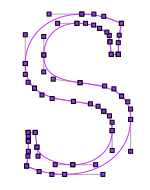
\includegraphics{letter}
\caption{A letter $S$.}
\label{F:Letter_S}
\end{figure}


\csection{Introduction}
\label{sec:indep_intro}

In Section \ref{sec:vector_representation} we saw how to represent water-benzene-acetic acid chemical solutions with vectors, where the components represent the water, benzene and acid percentages.  We then considered a problem of determining if a given chemical solution could be made by mixing other chemical solutions. Suppose we now have three different water-benzene-acetic acid chemical solutions, one with 40\% water, 50\% benzene and 10\% acetic acid, the second with 52\% water, 42\% benzene and 6\% acid, and a third with 46\% water, 46\% benzene and 8\% acid. We represent the first chemical solution with the vector $\vv_1 = \left[ \begin{array}{c} 40\\50\\10\end{array} \right]$, the second with the vector $\vv_2 = \left[ \begin{array}{c} 52\\42\\6\end{array} \right]$, and the third with the vector $\vv_3 = \left[ \begin{array}{c} 46\\46\\8\end{array} \right]$. By combining these three chemical solutions we can make a chemical solution with 43\% water, 48\% benzene and 9\% acid as follows
\[\frac{7}{12}\vv_1 + \frac{1}{12} \vv_2 + \frac{1}{3}\vv_3 = \left[ \begin{array}{c} 43\\48\\9\end{array} \right].\]
However, if we had noticed that the third chemical solution can actually be made from the first two, that is,
\[\frac{1}{2}\vv_1 + \frac{1}{2} \vv_2 = \vv_3,\]
we might have realized that we don't need the third chemical solution to make the 43\% water, 48\% benzene and 9\% acid chemical solution. In fact, 
\[\frac{3}{4}\vv_1 + \frac{1}{4} \vv_2 = \left[ \begin{array}{c} 43\\48\\9\end{array} \right].\]
(See Exercise \ref{ex:1_d_acid} of Section \ref{sec:vector_representation}.) Using the third chemical solution (represented by $\vv_3$) uses more information than we actually need to make the desired 43\% water, 48\% benzene and 9\% acid chemical solution because the vector $\vv_3$ is redundant -- all of the material we need to make $\vv_3$ is contained in $\vv_1$ and $\vv_2$. This is the basic idea behind linear independence -- representing information in the most efficient way.

Information is often contained in and conveyed through vectors -- especially linear combinations of vectors. In this section we will investigate the concepts of linear dependence and independence of a set of vectors. Our goal is to be able to efficiently determine when a given set of vectors forms a \emph{minimal spanning set}. A minimal spanning set is a spanning set that contains the smallest number of vectors to obtain all of the vectors in the span. An important aspect of a minimal spanning set is that every vector in the span can be written in one and only one way as a linear combination of the vectors in the minimal spanning set. This will allow us to define the important notion of the dimension of a vector space. \\

\noindent \textbf{Review of useful information:} Recall that a linear combination of vectors $\vv_1$, $\vv_2$, $\ldots$, $\vv_k$ in $\R^n$ is a sum of scalar multiples of $\vv_1$, $\vv_2$, $\ldots$, $\vv_k$. That is, a linear combination of the vectors $\vv_1$, $\vv_2$, $\ldots$, $\vv_k$ is a vector of the form
\[c_1\vv_1 + c_2\vv_2 + \cdots + c_k\vv_k,\]
where $c_1$, $c_2$, $\ldots$, $c_k$ are scalars.

Recall also that the collection of all linear combinations of a set $\{\vv_1$, $\vv_2$, $\ldots$, $\vv_k\}$ of vectors in $\R^n$ is called the span of the set of vectors. That is, the span $\Span \{\vv_1, \vv_2, \ldots, \vv_k\}$ of the set $\vv_1$, $\vv_2$, $\ldots$, $\vv_k$ of vectors in $\R^n$ is the set
\[ \{c_1\vv_1 + c_2\vv_2 + \cdots + c_k\vv_k : \text{ where } c_1, c_2, \ldots, c_k \text{ are scalars}\}.\]

For example, a linear combination of vectors $\vv_1 = \left[ \begin{array}{c} 1\\1\\2 \end{array} \right]$ and $\vv_2 = \left[ \begin{array}{r} 0\\-2\\1 \end{array} \right]$ is $2 \vv_1-3\vv_2 = \left[ \begin{array}{c} 2\\8\\1 \end{array} \right]$. All linear combinations of these two vectors can be expressed as the collection of vectors of the form $\left[ \begin{array}{c} c_1\\c_1-2c_2\\2c_1+c_2 \end{array} \right]$ where $c_1, c_2$ are scalars. Suppose we want to determine whether $\vw=\left[ \begin{array}{c} 1\\2\\3 \end{array} \right]$ is in the span, in other words if $\vw$ is a linear combination of $\vv_1, \vv_2$. This means we are looking for $c_1, c_2$ such that 
\[  \left[ \begin{array}{c} c_1\\c_1-2c_2\\2c_1+c_2 \end{array} \right] = \left[ \begin{array}{c} 1\\2\\3 \end{array} \right] \, . \]
 we solve for the system represented with the augmented matrix 
\[ \left[\begin{array}{crc|c} 1&0&&1\\ 1&-2&&2 \\ 2&1&&3\end{array} \right] \,. \]
By reducing this matrix, we find that there are no solutions of the system, which implies that $\vw$ is not a linear combination of $\vv_1, \vv_2$. Note that we can use any names we please for the scalars, say $x_1, x_2$, if we prefer.



\begin{pa} \label{pa:1_f} Let $\vv_1 = \left[ \begin{array}{r} 2\\1\\-3 \end{array} \right]$, $\vv_2 =  \left[ \begin{array}{c} 1\\1\\0 \end{array} \right]$, and $\vv_3 = \left[ \begin{array}{r} 1\\-1\\-6 \end{array} \right]$, and let $\vb = \left[ \begin {array}{c} 0 \\ 1 \\ 3 \end {array} \right]$. If $\vb$ is in $\Span \{\vv_1, \vv_2, \vv_3\}$, we are interested in the most efficient way to represent $\vb$ as a linear combination of $\vv_1$, $\vv_2$, and $\vv_3$. 
\be
\item \label{act:PA1_f_1} The vector $\vb$ is in $\Span \{\vv_1, \vv_2, \vv_3\}$ if there exist $x_1$, $x_2$, and $x_3$ so that 
\[x_1 \vv_1 + x_2 \vv_2 + x_3 \vv_3 = \vb.\]
(Recall that we can use any letters we want for the scalars. They are simply unknown scalars we want to solve for.)
	\ba
	\item Explain why $\vb$ is in $\Span \{\vv_1, \vv_2, \vv_3\}$. (Hint: What is the matrix we need to reduce?) 


	\item Write $\vb$ as a linear combination of $\vv_1$, $\vv_2$, and $\vv_3$. In how many ways can $\vb$ be written as a linear combination of the vectors $\vv_1$, $\vv_2$, and $\vv_3$? Explain. 


	\ea



\item \label{act:PA1_f_2}  In problem \ref{act:PA1_f_1} we saw that the vector $\vb$ could be written in infinitely many different ways as linear combinations of $\vv_1$, $\vv_2$, and $\vv_3$. We now ask the question if we really need all of the vectors $\vv_1$, $\vv_2$, and $\vv_3$ to make $\vb$ as a linear combination in a unique way.  
	\ba
	\item Can the vector $\vb$ be written as a linear combination of the vectors $\vv_1$ and $\vv_2$? If not, why not? If so, in how many ways can $\vb$ be written as a linear combination of $\vv_1$ and $\vv_2$? Explain.


	\item If possible, write $\vb$ as a linear combination of $\vv_1$ and $\vv_2$.  


	\ea


\item In problem \ref{act:PA1_f_1} we saw that $\vb$ could be written in infinitely many different ways as a linear combination of the vectors $\vv_1$, $\vv_2$, and $\vv_3$. However, the vector $\vb$ could only be written in one way as a linear combination of $\vv_1$ and $\vv_2$. So $\vb$ is in $\Span \{\vv_1, \vv_2, \vv_3\}$ and $\vb$ is also in $\Span \{\vv_1, \vv_2\} $. This raises a question -- is \emph{any} vector in $\Span \{\vv_1, \vv_2, \vv_3\}$ also in $\Span\{\vv_1, \vv_2\}$. If so, then the vector $\vv_3$ is redundant in terms of forming the span of $\vv_1$, $\vv_2$, and $\vv_3$. For the sake of efficiency, we want to recognize and eliminate this redundancy.  
 
	\ba
	\item Can $\vv_3$ be written as a linear combination of the vectors $\vv_1$ and $\vv_2$? If not, why not? If so, write $\vv_3$ as a linear combination of $\vv_1$ and $\vv_2$. 
	
	
	\item Use the result of part (a) to decide if \emph{any} vector in $\Span\{\vv_1, \vv_2, \vv_3\}$ is also in $\Span\{\vv_1, \vv_2\}$. 


\ea

\ee

\end{pa}

\csection{Linear Independence}
\label{sec:lin_indep}

In this section we will investigate the concepts of linear dependence and independence of a set of vectors. Our goal is to be able to efficiently determine when a given set of vectors forms a \emph{minimal spanning set}. This will involve the concepts of span and linear independence. Minimal spanning sets are important in that they provide the most efficient way to represent vectors in a space, and will later allow us to define the dimension of a vector space.  


In Preview Activity \ref{pa:1_f} we considered the case where we had a set $\{\vv_1, \vv_2, \vv_3\}$ of three vectors, and the vector $\vv_3$ was in the span of $\{\vv_1, \vv_2\}$. So the the vector $\vv_3$ did not add anything to the span of $\{\vv_1, \vv_2\}$. In other words, the set $\{\vv_1, \vv_2, \vv_3\}$ was larger than it needed to be in order to generate the vectors in its span -- that is, $\Span\{\vv_1, \vv_2, \vv_3\} = \Span \{\vv_1, \vv_2\}$. However, neither of the vectors in the set $\{\vv_1, \vv_2\}$ could be removed without changing its span. In this case, the set $\{\vv_1, \vv_2\}$ is what we will call a \emph{minimal spanning set}\index{minimal spanning set} or a \emph{basis} for $\Span \ S$. There are two important properties that make $\{\vv_1, \vv_2\}$ a basis for $\Span \ S$. The first is that every vector in $\Span \ S$ can be written as linear combinations of $\vv_1$ and $\vv_2$ (we also use the terminology that the vectors $\vv_1$ and $\vv_2$ span $\Span \ S$), and the second is that every vector in $\Span \ S$ can be written in exactly one way as a linear combination of $\vv_1$ and $\vv_2$. This second property is the property of linear independence, and it is the property that makes the spanning set \emph{minimal}. 

To make a spanning set minimal, we want to be able to write every vector in the span in a unique way in terms of the spanning vectors. Notice that the zero vector can always be written as a linear combination of any set of vectors using 0 for all of the weights. So to have a \emph{minimal} or \emph{linearly independent} spanning set, that is, to have a unique representation for each vector in the span, it will need to be the case that the \emph{only} way we can write the zero vector as a linear combination of a set of vectors is if all of the weights are 0. This leads us to the definition of a linearly independent set of vectors.  


\begin{definition} \label{def:linear_independence_Rn} A set $\{\vv_1, \vv_2, \ldots, \vv_k\}$ of vectors in $\R^n$ is \textbf{linearly independent}\index{linear independence} if the vector equation
\[x_1 \vv_1 + x_2 \vv_2 + \cdots + x_k \vv_k = \vzero\]
for scalars $x_1, x_2, \ldots, x_k$ has only the trivial solution
\[x_1 = x_2 = x_3 = \cdots = x_k = 0.\]
If a set of vectors is not linearly independent, then the set is \textbf{linearly dependent}\index{linear dependence}.
\end{definition}

Alternatively, we say that the vectors $\vv_1, \vv_2, \ldots, \vv_k$ are linearly independent (or dependent) if the set $\{\vv_1, \vv_2, \ldots, \vv_k\}$ is linearly independent (or dependent).


Note that the definition tells us that a set $\{\vv_1, \vv_2, \ldots, \vv_k\}$ of vectors in $\R^n$ is linearly dependent if there are scalars $x_1$, $x_2$, $\ldots$, $x_n$, not all of which are 0 so that
\[x_1 \vv_1 + x_2 \vv_2 + \cdots + x_k \vv_k = \vzero.\]


\begin{activity} \label{act:1_f_1} Which of the following sets in $\R^2$ or $\R^3$ is linearly independent and which is linearly dependent? Why? For the linearly dependent sets, write one of the vectors as a linear combination of the others, if possible. 
\ba
\item $S_1 = \left\{\left[\begin{array}{c} 2 \\ 0 \\ 1 \end{array}\right], \left[\begin{array}{r} -2 \\ 8 \\ 1 \end{array}\right], \left[\begin{array}{r} -4 \\ 8 \\ 0 \end{array}\right]\right\}$.



\item $S_2 = \left\{\left[\begin{array}{c} 1 \\ 2 \\ 1 \end{array}\right], \left[\begin{array}{c} 0 \\ 2 \\ 3 \end{array}\right]\right\}$. (Hint: What relationship must exist between two vectors if they are linearly dependent?)



\item The vectors $\vu$, $\vv$, and $\vw$ as shown in Figure \ref{F:1_f_1}.
\begin{figure}[ht]
\begin{center}
\resizebox{!}{2.0in}{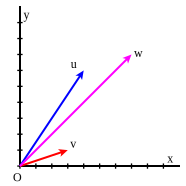
\includegraphics{1_f_lin_dependence}}
\caption{Vectors $\vu$, $\vv$, and $\vw$.}
\label{F:1_f_1}
\end{center}
\end{figure}


\ea

\end{activity}


Activity \ref{act:1_f_1} (a) and (c) illustrate how we can write one of the vectors in a linearly dependent set as a linear combination of the others. This would allow us to write at least one of the vectors in the span of the set in more than one way as a linear combination of vectors in this set. We prove this result in general in the following theorem.

\begin{theorem} \label{thm:Dependence} A set $\{\vv_1, \vv_2, \ldots, \vv_k\}$ of vectors in $\R^n$ is linearly dependent if and only if at least one of the vectors in the set can be written as a linear combination of the remaining vectors in the set.
\end{theorem}

The next activity is intended to help set the stage for the proof of Theorem \ref{thm:Dependence}. 

\begin{activity} \label{act:1_f_1b} The statement of Theorem \ref{thm:Dependence} is a bi-conditional statement (an if and only if statement). To prove this statement about the set $S$ we need to show two things about $S$. One: we must demonstrate that if $S$ is a linearly dependent set, then at least one vector in $S$ is a linear combination of the other vectors (this is the ``only if" part of the biconditional statement) and Two: if at least one vector in $S$ is a linear combination of the others, then $S$ is linearly dependent (this is the ``if" part of the biconditional statement). We illustrate the main idea of the proof using a three vector set $S = \{\vv_1, \vv_2, \vv_3\}$. 
	\ba
	\item First let us assume that $S$ is a linearly dependent set and show that at least one vector in $S$ is a linear combination of the other vectors. Since $S$ is linearly dependent we can write the zero vector as a linear combination of $\vv_1$, $\vv_2$, and $\vv_3$ with at least one nonzero weight. For example, suppose 
\begin{equation} \label{eq:1_f_dependence_thm_1}
2\vv_1 + 3\vv_2 + 4\vv_3 = \vzero.
\end{equation}
Solve Equation (\ref{eq:1_f_dependence_thm_1}) for the vector $\vv_2$ to show that $\vv_2$ can be written as a linear combination of $\vv_1$ and $\vv_3$. Conclude that $\vv_2$ is a linear combination of the other vectors in the set $S$. 

	\item Now we assume that at least one of the vectors in $S$ is a linear combination of the others. For example, suppose that
\begin{equation} \label{eq:1_f_dependence_thm_2}
 \vv_3 = \vv_1 + 5\vv_2.
\end{equation}
Use vector algebra to rewrite Equation \ref{eq:1_f_dependence_thm_2} so that $\vzero$ is expressed as a linear combination of $\vv_1$, $\vv_2$, and $\vv_3$ such that the weight on $\vv_3$ is not zero. Conclude that the set $S$ is linearly dependent. 

	\ea
	
\end{activity}

Now we provide a formal proof of Theorem \ref{thm:Dependence}, using the ideas from Activity \ref{act:1_f_1b}.

\begin{proof}[Proof of Theorem \ref{thm:Dependence}] Let $S = \{\vv_1, \vv_2, \ldots, \vv_k\}$ be a set of vectors in $\R^n$.  We will begin by verifying the first statement.

We assume that $S$ is a linearly dependent set and show that at least one vector in $S$ is a linear combination of the others. Since $S$ is linearly dependent, there are scalars $x_1$, $x_2$, $\ldots$, $x_n$, not all of which are 0, so that 
\begin{equation} \label{eq:1_f_dependence_1} 
x_1\vv_1 + x_2\vv_2 + \cdots +  x_{k}\vv_{k} = \vzero.
\end{equation}
We don't know which scalar(s) are not zero, but there is at least one. So let us assume that $x_i$ is not zero for some $i$ between 1 and $k$.  We can then subtract $x_i \vv_i$ from both sides of Equation (\ref{eq:1_f_dependence_1}) and divide by $x_i$ to obtain
\[\vv_i = \frac{x_1}{x_i}\vv_1 + \frac{x_2}{x_i}\vv_2 + \cdots + \frac{x_{i-1}}{x_i}\vv_{i-1} +  \frac{x_{i+1}}{x_i}\vv_{i+1} + \frac{x_{i+2}}{x_i}\vv_{i+2} + \cdots + \frac{x_{k}}{x_i}\vv_{k}.\]
Thus, the vector $\vv_i$ is a linear combination of $\vv_1$, $\vv_2$, $\ldots$, $\vv_{i-1}$, $\vv_{i+1}$, $\ldots$, $\vv_k$, and at least one of the vectors in $S$ is a linear combination of the other vectors in $S$. 

To verify the second statement, we assume that at least one of the vectors in $S$ can be written as a linear combination of the others and show that $S$ is then a linearly dependent set. We don't know which vector(s) in $S$ can be written as a linear combination of the others, but there is at least one. Let us suppose that $\vv_i$ is a linear combination of the vectors $\vv_1$, $\vv_2$, $\ldots$, $\vv_{i-1}$, $\vv_{i+1}$, $\ldots$, $\vv_k$ for some $i$ between 1 and $k$. Then there exist scalars  $x_1$, $x_2$, $\ldots$, $x_{-1}$, $x_{i+1}$, $\ldots$, $x_n$ so that 
\[\vv_i = x_1\vv_1 + x_2\vv_2 + \cdots + x_{i-1}\vv_{i-1} +  x_{i+1}\vv_{i+1} + x_{i+2}\vv_{i+2} + \cdots + x_{k}\vv_{k}.\]
It follows that 
\[\vzero = x_1\vv_1 + x_2\vv_2 + \cdots + x_{i-1}\vv_{i-1} +  (-1)\vv_i + x_{i+1}\vv_{i+1} + x_{i+2}\vv_{i+2} + \cdots + x_{k}\vv_{k}.\] 
So there are scalars there are scalars $x_1$, $x_2$, $\ldots$, $x_n$ (with $x_i = -1$), not all of which are 0, so that 
\[x_1\vv_1 + x_2\vv_2 + \cdots +  x_{k}\vv_{k} = \vzero.\]
This makes $S$ a linearly dependent set. 
\end{proof}

With a linearly dependent set, at least one of the vectors in the set is a linear combination of the others. With a linearly independent set, this cannot happen -- no vector in the set can be written as a linear combination of the others. This result is given in the next theorem. You may be able to see how Theorems \ref{thm:Dependence} and \ref{thm:Independence} are logically equivalent.  


\begin{theorem} \label{thm:Independence} A set $\{\vv_1, \vv_2, \ldots, \vv_k\}$ of vectors in $\R^n$ is linearly independent if and only if no vector in the set can be written as a linear combination of the remaining vectors in the set.
\end{theorem}


\begin{activity} \label{act:1_f_2}  As was hinted at in Preview Activity \ref{pa:1_f}, an important consequence of a linearly independent set is that every vector in the span of the set can be written in one and only one way as a linear combination of vectors in the set. It is this uniqueness that makes linearly independent sets so useful. We explore this idea in this activity for a linearly independent set of three vectors. Let $S = \{\vv_1, \vv_2, \vv_3\}$ be a linearly independent set of vectors in $\R^n$ for some $n$, and let $\vb$ be a vector in $\Span \ S$. To show that $\vb$ can be written in exactly one way as a linear combination of vectors in $S$, we assume that 
\[\vb = x_1 \vv_1 + x_2 \vv_2 + x_3 \vv_3 \ \ \text{ and } \ \ \vb = y_1\vv_1 + y_2 \vv_2 + y_3 \vv_3\]
for some scalars $x_1$, $x_2$, $x_3$, $y_1$, $y_2$, and $y_3$. We need to demonstrate that $x_1=y_1$, $x_2=y_2$, and  $x_3=y_3$. 
	\ba
	\item Use the two different ways of writing $\vb$ as a linear combination of $\vv_1, \vv_2$ and $\vv_3$ to come up with a linear combination expressing $\vzero$ as a linear combination of these vectors.	
	
	\item Use the linear independence of the vectors $\vv_1, \vv_2$ and $\vv_3$ to explain why $x_1=y_1$, $x_2=y_2$, and  $x_3=y_3$.
	
	\ea
\end{activity}



Activity \ref{act:1_f_2} contains the general ideas to show that any vector in the span of a linearly independent set can be written in one and only one way as a linear combination of the vectors in the set. The weights of such a linear combination provide us a \emph{coordinate system} for the vectors in terms of the basis. Two familiar examples of coordinate systems are the Cartesian coordinates in the $xy$-plane, and $xyz$-space. We will revisit the coordinate system idea in a later chapter. 

In the next theorem we state and prove the general case of any number of linearly independent vectors producing unique representations as linear combinations.



\begin{theorem} \label{thm:1_f_unique_representation} Let $S = \{\vv_1, \vv_2, \ldots, \vv_k\}$ be a linearly independent set of vectors in $\R^n$. Any vector in $\Span \ S$ can be written in one and only one way as a linear combination of the vectors $\vv_1$, $\vv_2$, $\ldots$, $\vv_k$.  
\end{theorem}

\begin{proof} Let $S = \{\vv_1, \vv_2, \ldots, \vv_k\}$ be a linearly independent set of vectors in $\R^n$, and let $\vb$ be a vector in $\Span \ S$. By definition, it follows that $\vb$ can be written as a linear combination of the vectors in $S$. It remains for us to show that this representation is unique. So assume that 
\begin{equation} \label{eq:1_f_1} 
\vb = x_1 \vv_1 + x_2 \vv_2 + \cdots + x_k \vv_k \ \ \text{ and } \ \ \vb = y_1\vv_1 + y_2 \vv_2 + \cdots + y_k \vv_k
\end{equation}
for some scalars $x_1$, $x_2$, $\ldots$, $x_k$, and $y_1$, $y_2$, $\ldots$, $y_k$. Then 
\[x_1 \vv_1 + x_2 \vv_2 + \cdots + x_k \vv_k = y_1\vv_1 + y_2 \vv_2 + \cdots + y_k \vv_k.\]
Subtracting all terms from the right side and using a little vector algebra gives us 
\[(x_1-y_1) \vv_1 + (x_2-y_2) \vv_2 + \cdots + (x_k-y_k) \vv_k = \vzero.\]
 The fact that $S$ is a linearly independent set implies that 
 \[x_1-y_1=0, \ x_2-y_2 = 0, \ \ldots, \ x_k-y_k=0,\]
showing that $x_i=y_i$ for every $i$ between 1 and $k$. We conclude that the representation of $\vb$ as a linear combination of the linearly independent vectors in $S$ is unique. 

\end{proof}


\csection{Determining Linear Independence}
\label{sec:determ_lin_ind}

The definition and our previous work give us a straightforward method for determining when a set of vectors in $\R^n$ is linearly independent or dependent.  



\begin{activity} \label{act:1_f_3} In this activity we learn how to use a matrix to determine in general if a set of vectors in $\R^n$ is linearly independent or dependent. Suppose we have $k$ vectors $\vv_1$, $\vv_2$, $\ldots$, $\vv_k$ in $\R^n$. To see if these vectors are linearly independent, we need to find the solutions to the vector equation
\begin{equation} \label{eq:lin_indep}
x_1 \vv_1 + x_2 \vv_2 + \cdots + x_k \vv_k = \vzero.
\end{equation}
If we let $A = [\vv_1 \  \vv_2 \ \vv_3 \ \cdots \ \vv_k]$ and $\vx = \left[ \begin{array}{c} x_1 \\ x_2 \\ \vdots \\ x_k \end{array} \right]$, then we can write the vector equation (\ref{eq:lin_indep}) in matrix form $A \vx = \vzero$. Let $B$ be the reduced row echelon form of $A$.
	\ba
	\item  What can we say about the pivots of $B$ in order for $A \vx = \vzero$ to have exactly one solution? Under these conditions, are the vectors $\vv_1$, $\vv_2$, $\ldots$, $\vv_k$ linearly independent or dependent? 

	
	
	\item What can we say about the rows or columns of $B$ in order for $A \vx = \vzero$ to have infinitely many solutions? Under these conditions, are the vectors $\vv_1$, $\vv_2$, $\ldots$, $\vv_k$ linearly independent or dependent? 
	
	
	
	\item Use the result of parts (a) and (b) to determine if the vectors $\vv_1 = \left[ \begin{array}{r} 1 \\ -1 \\ 2 \\ 0 \end{array} \right]$, $\vv_2 = \left[ \begin{array}{c} 1 \\ 0 \\ 2 \\ 3 \end{array} \right]$, and $\vv_3 = \left[ \begin{array}{c} 0 \\ 0 \\ 2 \\ 1 \end{array} \right]$ in $\R^4$ are linearly independent or dependent. If dependent, write one of the vectors as a linear combination of the others. You may use the fact that the matrix $\left[ \begin{array}{rcc} 1&1&0 \\ -1&0&0 \\ 2&2&2 \\ 0&3&1 \end{array} \right]$ is row equivalent to $\left[ \begin{array}{rcc} 1&0&0 \\ 0&1&0 \\ 0&0&1 \\ 0&0&0 \end{array} \right]$.



\ea

\end{activity}

\csection{Minimal Spanning Sets}
\label{sec:min_span_set}

It is important to note the differences and connections between linear independence, span, and minimal spanning set. 
\begin{itemize}
\item The set $S = \left\{ \left[ \begin{array}{c} 1 \\ 0 \\ 0 \end{array} \right], \left[ \begin{array}{c} 0 \\ 1 \\ 0 \end{array} \right] \right\}$ is not a minimal spanning set for $\R^3$ even though $S$ is a linearly independent set. Note that $S$ does not span $\R^3$ since the vector $\left[ \begin{array}{c} 0 \\ 0 \\ 1 \end{array} \right] $ is not in $\Span \ S$. 
\item The set $T = \left\{ \left[ \begin{array}{c} 1 \\ 0 \\ 0 \end{array} \right], \left[ \begin{array}{c} 0 \\ 1 \\ 0 \end{array} \right] , \left[ \begin{array}{c} 0 \\ 0 \\ 1 \end{array} \right] , \left[ \begin{array}{c} 1 \\ 1 \\ 1 \end{array} \right] \right\}$ is not a minimal spanning set for $\R^3$ even though $\Span \ T = \R^3$. Note that 
\[\left[ \begin{array}{c} 1 \\ 1 \\ 1 \end{array} \right] = \left[ \begin{array}{c} 1 \\ 0 \\ 0 \end{array} \right] + \left[ \begin{array}{c} 0 \\ 1 \\ 0 \end{array} \right] + \left[ \begin{array}{c} 0 \\ 0 \\ 1 \end{array} \right], \]
so $T$ is not a linearly independent set.
\item The set $U = \left\{ \left[ \begin{array}{c} 1 \\ 0 \\ 0 \end{array} \right], \left[ \begin{array}{c} 0 \\ 1 \\ 0 \end{array} \right] , \left[ \begin{array}{c} 0 \\ 0 \\ 1 \end{array} \right]  \right\}$ is a minimal spanning set for $\R^3$ since it satisfies both characteristics of a minimal spanning set: $\Span \ U = \R^3$ AND $U$ is linearly independent. 
\end{itemize}
The three concepts -- linear independence, span, and minimal spanning set -- are different. The important point to note is that minimal spanning set must be both linearly independent and span the space. 

To find a minimal spanning set we will often need to find a smallest subset of a given set of vectors that has the same span as the original set of vectors. In this section we determine a method for doing so. 

\begin{activity} \label{act:1_f_4} Let $\vv_1 = \left[ \begin{array}{r} -1 \\ 0 \\ 2 \end{array} \right]$, $\vv_2 = \left[ \begin{array}{r} 2 \\ 0 \\ -4 \end{array} \right]$, $\vv_3 = \left[ \begin{array}{c} 0 \\ 1 \\ 3 \end{array} \right]$, and $\vv_4 = \left[ \begin{array}{r} -3 \\ 4 \\ 18 \end{array} \right]$ in $\R^3$. Assume that the reduced row echelon form of the matrix $A = \left[ \begin{array}{rrcr} -1&2&0&-3 \\ 0&0&1&4 \\ 2&-4&3&18 \end{array} \right]$ is $\left[ \begin{array}{crcc} 1&-2&0&3 \\ 0&0&1&4 \\ 0&0&0&0 \end{array} \right]$. 
	\ba
	\item Write the general solution to the homogeneous system $A \vx = \vzero$, where $\vx = \left[ \begin{array}{c} x_1 \\ x_2 \\ x_3 \\ x_4 \end{array} \right]$. Write all linear combinations of $\vv_1$, $\vv_2$, $\vv_3$, and $\vv_4$ that are equal to $\vzero$, using weights that only involve $x_2$ and $x_4$. 
	
	
	
	\item Explain how we can conveniently choose the weights in the general solution to $A \vx = \vzero$ to show that the vector $\vv_4$ is a linear combination of $\vv_1$, $\vv_2$, and $\vv_3$. What does this tell us about $\Span \{\vv_1, \vv_2, \vv_3\}$ and $\Span \{\vv_1, \vv_2, \vv_3, \vv_4\}$? 
	
	
	
	\item Explain how we can conveniently choose the weights in the general solution to $A \vx = \vzero$ to show why the vector $\vv_2$ is a linear combination of $\vv_1$ and $\vv_3$. What does this tell us about $\Span \{\vv_1, \vv_3\}$ and $\Span \{\vv_1, \vv_2, \vv_3 \}$?
	
	
	
	\item Is $\{\vv_1, \vv_3\}$ a minimal spanning set for $\Span \{\vv_1, \vv_2, \vv_3, \vv_4\}$? Explain your response. 
	
	
	
	
	\ea
\end{activity}



Activity \ref{act:1_f_4} illustrates how we can use a matrix to determine a minimal spanning set for a given set of vectors $\{\vv_1, \vv_2, \ldots, \vv_k\}$ in $\R^n$.
\begin{itemize}
\item Form the matrix $A = [\vv_1 \ \vv_2 \ \cdots \ \vv_k]$.
\item Find the reduced row echelon form $[B \ | \ \vzero]$ of $[A \ | \ \vzero]$. If $B$ contains non-pivot columns, say for example that the $i$th column is a non-pivot column, then we can choose the weight $x_i$ corresponding to the $i$th column to be 1 and all weights corresponding to the other non-pivot columns to be 0 to make a linear combination of the columns of $A$ that is equal to $\vzero$. This allows us to write $\vv_i$ as a linear combination of the vectors corresponding to the pivot columns of $A$ as we did in the proof of Theorem \ref{thm:Independence}. So every vector corresponding to a non-pivot column is in the span of the set of vectors corresponding to the pivot columns. The vectors corresponding to the pivot columns are linearly independent, since the matrix with those columns has every column as a pivot column. Thus, the set of vectors corresponding to the pivot columns of $A$ forms a minimal spanning set for $\{\vv_1, \vv_2, \ldots, \vv_k\}$.
\end{itemize}

\noindent \textbf{IMPORTANT NOTE!} The set of pivot columns of the reduced row echelon form of $A$ will normally not have the same span as the set of columns of $A$, so it is critical that we use columns of $A$, NOT $B$ in our minimal spanning set.



\begin{activity} \label{act:1_f_5} Find a minimal spanning set for the span of the set 
\[\left\{ \left[ \begin{array}{c} 1 \\ 1 \\ 0 \\ 0 \end{array} \right], \left[ \begin{array}{c} 2 \\ 3 \\ 0 \\ 0 \end{array} \right], \left[ \begin{array}{c} 0 \\ 1 \\ 2 \\ 0 \end{array} \right], \left[ \begin{array}{c} 4 \\ 1 \\ 0 \\ 0 \end{array} \right] \right\}.\] 



\end{activity}

Activity \ref{act:1_f_4} also illustrates a general process by which we can find a minimal spanning set -- that is the smallest subset of vectors that has the same span. This process will be useful later when we consider vectors in arbitrary vector spaces. The idea is that if we can write one of the vectors in a set $S$ as a linear combination of the remaining vectors, then we can remove that vector from the set and maintain the same span. In other words, begin with the span of a set $S$ and follow these steps:
\begin{description}
\item[Step 1.] If $S$ is a linearly independent set, we already have a minimal spanning set.
\item[Step 2.] If $S$ is not a linearly independent set, then one of the vectors in $S$ is a linear combination of the others. Remove that vector from $S$ to obtain a new set $T$. It will be the case that $\Span \ T = \Span \ S$.
\item[Step 3.] If $T$ is a linearly independent set, then $T$ is a minimal spanning set. If not, repeat steps 2 and 3 for the set $T$ until you arrive at a linearly independent set.
\end{description}
This process is guaranteed to stop as long as the set contains at least one nonzero vector. A verification of the statement in Step 2 that $\Span \ T = \Span \ S$ is given in the next theorem.



\begin{theorem} \label{thm:minimal_spanning_set} Let $\{\vv_1, \vv_2, \ldots, \vv_k\}$ be a set of vectors in $\R^n$ so that for some $i$ between 1 and $k$, $\vv_i$ is in $\Span \{\vv_1, \vv_2, \ldots, \vv_{i-1}, \vv_{i+1}, \ldots, \vv_k\}$. Then
\[\Span \{\vv_1, \vv_2, \ldots, \vv_k\} = \Span \{\vv_1, \vv_2, \ldots, \vv_{i-1}, \vv_{i+1}, \ldots, \vv_k\}.\]
\end{theorem}



\begin{proof} Let $\{\vv_1, \vv_2, \ldots, \vv_k\}$ be a set of vectors in $\R^n$ so that $\vv_i$ is in the span of $\vv_1$, $\vv_2$, $\ldots$, $\vv_{i-1}$, $\vv_{i+1}$, $\ldots$, and $\vv_k$ for some $i$ between 1 and $k$. To show that 
\[\Span \{\vv_1, \vv_2, \ldots, \vv_k\} = \Span \{\vv_1,  \ldots, \vv_{i-1}, \vv_{i+1}, \ldots, \vv_k\},\]
we need to show that
\begin{enumerate}
\item every vector in $\Span \{\vv_1, \vv_2, \ldots, \vv_k\}$ is in $\Span\{\vv_1, \ldots, \vv_{i-1}, \vv_{i+1}, \ldots, \vv_k\}$, and
\item every vector in $\Span \{\vv_1,  \ldots, \vv_{i-1}, \vv_{i+1}, \ldots, \vv_k\}$ is in \\ $\Span \{\vv_1, \ldots, \vv_k\}$.
\end{enumerate}
Let us consider the second containment. Let $\vx$ be a vector in the span of $\vv_1$, $\vv_2$, $\ldots$, $\vv_{i-1}$, $\vv_{i+1}$, $\ldots$, and $\vv_k$. Then
\[\vx = x_1\vv_1 + x_2\vv_2 + \cdots + x_{i-1}\vv_{i-1} + x_{i+1}\vv_{i+1} + \cdots + x_k\vv_k\]
for some scalars $x_1$, $x_2$, $\ldots$, $x_{i-1}$, $x_{i+1}$, $\ldots$, $x_k$. Note that
\[\vx = x_1\vv_1 + x_2\vv_2 + \cdots + x_{i-1}\vv_{i-1} + (0)\vv_i + x_{i+1}\vv_{i+1} + \cdots + x_k\vv_k\]
as well, so $\vx$ is in $\Span \{\vv_1, \vv_2, \ldots, \vv_k\}$. Thus, 
\[\Span \{\vv_1, \vv_2, \ldots, \vv_{i-1}, \vv_{i+1}, \ldots, \vv_k\} \subseteq  \Span \{\vv_1, \vv_2, \ldots, \vv_k\}.\]
(This same argument shows a more general statement that if $S$ is a subset of $T$, then $\Span \ S \subseteq \Span \ T$.)

Now we demonstrate the first containment. Here we need the assumption that $\vv_i$ is in $\Span \{\vv_1$, $\vv_2$, $\ldots$, $\vv_{i-1}$, $\vv_{i+1}$, $\ldots$, $\vv_k\}$ for some $i$ between 1 and $k$. That assumption gives us 
\begin{equation} \label{eq:lin_depend_containment}
\vv_i = c_1 \vv_1 + c_2\vv_2 + \cdots + c_{i-1}\vv_{i-1} + c_{i+1}\vv_{i+1} + \cdots + c_k\vv_k
\end{equation}
for some scalars $c_1$, $c_2$, $\ldots$, $c_{i-1}$, $c_{i+1}$, $\ldots$, $c_k$. Now let $\vx$ be a vector in the span of $\vv_1$, $\vv_2$, $\ldots$, $\vv_k$. Then
\[\vx = x_1\vv_1 + x_2\vv_2 + \cdots + x_k\vv_k\]
for some scalars $x_1$, $x_2$, $\ldots$, $x_k$. Substituting from (\ref{eq:lin_depend_containment}) shows that 
\begin{align*}
\vx &= x_1\vv_1 + x_2\vv_2 + \cdots + x_k\vv_k \\
	&= x_1\vv_1 + x_2\vv_2 + \cdots + x_{i-1} \vv_{i-1} + x_i \vv_i + x_{i+1}\vv_{i+1} + \cdots + x_k\vv_k \\
	&= x_1\vv_1 + x_2\vv_2 + \cdots + x_{i-1} \vv_{i-1} \\
	&\qquad + x_i[c_1 \vv_1 + c_2\vv_2 + \cdots + c_{i-1}\vv_{i-1} + c_{i+1}\vv_{i+1} + \cdots + c_k\vv_k]  \\
	&\qquad + x_{i+1}\vv_{i+1} + \cdots + x_k\vv_k \\
	&= (x_1+x_ic_1)\vv_1 + (x_2+x_ic_2)\vv_2 + \cdots + (x_{i-1}+x_ic_{i-1}) \vv_{i-1} \\
	&\qquad + (x_{i+1}+x_ic_{i+1}) \vv_{i+1} \cdots + (x_k+x_ic_k)\vv_k.
\end{align*}
So $\vx$ is in $\Span \{\vv_1, \vv_2, \ldots, \vv_{i-1}, \vv_{i+1}, \ldots, \vv_k\}$ and 
\[\Span \{\vv_1, \vv_2, \ldots, \vv_k\} \subseteq \Span \{\vv_1, \vv_2, \ldots, \vv_{i-1}, \vv_{i+1}, \ldots, \vv_k\}.\]
 Since the two sets are subsets of each other, they must be equal sets. We conclude that
\[\Span \{\vv_1, \vv_2, \ldots, \vv_k\} = \Span \{\vv_1, \vv_2, \ldots, \vv_{i-1}, \vv_{i+1}, \ldots, \vv_k\}.\]
\end{proof}



The result of Theorem \ref{thm:minimal_spanning_set} is that if we have a finite set $S$ of vectors in $\R^n$, we can eliminate those vectors that are linear combinations of others until we obtain a smallest set of vectors that still has the same span. As mentioned earlier, we call such a minimal spanning set a basis.



\begin{definition} \label{def:1_f_basis} Let $S$ be a set of vectors in $\R^n$. A subset $B$ of $S$ is a \textbf{basis}\index{basis} for $\Span \ S$ if $B$ is linearly independent and $\Span \ B = \Span \ S$. 
\end{definition}



\noindent \textbf{IMPORTANT NOTE: } A basis is defined by two characteristics. A basis must span the space in question and a basis must be a linearly independent set. It is the linear independence that makes a basis a \emph{minimal} spanning set. 

We have worked with a familiar basis in $\R^2$ throughout our mathematical careers. A vector $\left[ \begin{array}{c} a \\ b \end{array} \right]$ in $\R^2$ can be written as 
\[\left[ \begin{array}{c} a \\ b \end{array} \right] = a\left[ \begin{array}{c} 1 \\ 0 \end{array} \right] + b\left[ \begin{array}{c} 0 \\ 1 \end{array} \right].\]
So the set $\{\ve_1, \ve_2\}$, where $\ve_1 = \left[ \begin{array}{c} 1 \\ 0 \end{array} \right]$ and $\ve_2 = \left[ \begin{array}{c} 0 \\ 1 \end{array} \right]$ spans $\R^2$. Since the columns of $[\ve_1 \ \ve_2]$ are linearly independent, so is the set $\{\ve_1, \ve_2\}$. Therefore, the set $\{\ve_1, \ve_2\}$ is a basis for $\R^2$. The vector $\ve_1$ is in the direction of the positive $x$-axis and the vector $\ve_2$ is in the direction of the positive $y$-axis, so decomposing a vector $\left[ \begin{array}{c} a \\ b \end{array} \right]$ as a linear combination of $\ve_1$ and $\ve_2$ is akin to identifying the vector with the point $(a,b)$ as we discussed earlier. The set $\{\ve_1, \ve_2\}$ is called the \emph{standard basis} for $\R^2$. 

This idea is not restricted to $\R^2$. Consider the vectors 
\[\ve_1 = \left[ \begin{array}{c} 1\\0\\0 \\ \vdots \\ 0 \\ 0 \end{array} \right], \ \ve_2 = \left[ \begin{array}{c} 0\\1\\0 \\ \vdots \\ 0 \\ 0 \end{array} \right], \ \cdots, \ \ve_n = \left[ \begin{array}{c} 0\\0\\0 \\ \vdots \\ 0 \\ 1 \end{array} \right]\]
in $\R^n$. That is, the vector $\ve_i$ is the vector with a 1 in the $i$th position and 0s everywhere else. Since the matrix $[\ve_1 \ \ve_2 \ \cdots \ \ve_n]$ has a pivot in each row and column, the set $\{\ve_1, \ve_2, \ldots, \ve_n\}$ is a basis for $\R^n$. The set $\{\ve_1, \ve_2, \ldots, \ve_n\}$ is called the \emph{standard basis}\index{standard basis!for $\R^n$} for $\R^n$. 

As we will see later, bases\footnote{The plural of basis is bases.} are of fundamental importance in linear algebra in that bases will allow us to define the dimension of a vector space and will provide us with coordinate systems.   

We conclude this section with an important theorem that is similar Theorem \ref{thm:IMT_1_e}. 



\begin{theorem} \label{thm:IMT_1_f} Let $A$ be an $m \times n$ matrix. The following statements are equivalent.
    \begin{enumerate}
    \item The matrix equation $A \vx = \vb$ has a unique solution for every vector $\vb$ in the span of the columns of $A$.
    \item The matrix equation $A \vx = \vzero$ has the unique solution $\vx = \vzero$.
    \item The columns of $A$ are linearly independent.
    \item The matrix $A$ has a pivot position in each column. 
    \end{enumerate}
\end{theorem}




\csection{Examples}
\label{sec:indep_exam}

\ExampleIntro

\begin{example} Let $\vv_1 = \left[ \begin{array}{c} 1\\2\\0\\1 \end{array} \right]$, $\vv_2 = \left[ \begin{array}{r} 0\\6\\-1\\5 \end{array} \right]$, $\vv_3 = \left[ \begin{array}{r} 3\\-6\\2\\-7\end{array} \right]$, and $\vv_4 = \left[ \begin{array}{r} 5\\-2\\2\\-5 \end{array} \right]$.
	\ba
	\item Is the set $S = \{\vv_1, \vv_2, \vv_3, \vv_4\}$ linearly independent or dependent. If independent, explain why. If dependent, write one of the vectors in $S$ as a linear combination of the other vectors in $S$.
	
	\item Find a subset $B$ of $S$ that is a basis for $\Span \ S$. Explain how you know you have a basis.
	
	\ea
	
\ExampleSolution
\ba
\item We need to know the solutions to the vector equation
\[x_1 \vv_1 + x_2 \vv_2 + x_3 \vv_3 + x_4 \vv_4 = \vzero.\]
If the equation has as its only solution $x_1 = x_2 = x_3 = x_4 = 0$ (the trivial solution), then the set $S$ is linearly independent. Otherwise the set $S$ is linearly dependent.

To find the solutions to this system, we row reduce the augmented matrix
\[\left[ \begin{array}{crrr|c} 1&0&3&5&0 \\ 2&6&-6&-2&0 \\ 0&-1&2&2&0 \\ 1&5&-7&-5&0 \end{array} \right].\]
(Note that we really don't need the augmented column of zeros -- row operations won't change that column at all. We just need to know that the column of zeros is there.) Technology shows that the reduced row echelon form of this augmented matrix is 
\[\left[ \begin{array}{cccr|c} 1&0&3&5&0 \\ 0&1&-2&-2&0 \\ 0&0&0&0&0 \\ 0&0&0&0&0 \end{array} \right].\]
The reduced row echelon form tells us that the vector equation is consistent, and the fact that there is no pivot in the fourth column shows that the system has a free variable and more than just the trivial solution. We conclude that $S$ is linearly dependent. 

Moreover, the general solution to our vector equation is
\begin{align*}
x_1 &= -3x_3 - 5x_4 \\
x_2 &= 2x_3 + 2x_4 \\
x_3 &\text{ is free} \\
x_4 &\text{ is free}.
\end{align*}
Letting $x_4 = 0$ and $x_3 = 1$ shows that one non-trivial solution to our vector equation is
\[x_1 = -3, \ x_2 = 2, \ x_3 = 1, \ \text{ and } \ x_4 = 0.\]
Thus,
\[-3\vv_1 + 2\vv_2 + \vv_3 = \vzero,\]
or
\[\vv_3 = 3\vv_1 - 2\vv_2\]
and we have written one vector in $S$ as a linear combination of the other vectors in $S$. 

\item We have seen that the pivot columns in a matrix $A$ form a minimal spanning set (or basis) for the span of the columns of $A$. From part (a) we see that the pivot columns in the reduced row echelon form of $A = [\vv_1 \ \vv_2 \ \vv_3 \ \vv_4]$ are the first and second columns. So a basis for the span of the columns of $A$ is $\{\vv_1, \vv_2\}$. Since the elements of $S$ are the columns of $A$, we conclude that the set $B = \{\vv_1, \vv_2\}$ is a subset of $S$ that is a basis for $\Span \ S$. 

\ea
\end{example}

\begin{example} Let $\vv_1 = \left[ \begin{array}{c} 1 \\ 1 \\ 0 \end{array} \right]$, $\vv_2 = \left[ \begin{array}{r} 3 \\ -7 \\ 2 \end{array} \right]$, and $\vv_3 = \left[ \begin{array}{r} -5 \\ 6 \\ 10 \end{array} \right]$. 
	\ba
	\item Is the set $S = \left\{\vv_1, \vv_2, \vv_3\right\}$ a basis for $\R^3$? Explain. 
	
	\item Let $\vv_4 =  \left[ \begin{array}{r} -5 \\ 6 \\ h \end{array} \right]$, where $h$ is a scalar. Are there any values of $h$ for which the set $S' = \{\vv_1, \vv_2, \vv_4\}$ is not a basis for $\R^3$? If so, find all such values of $h$ and explain why $S'$ is not a basis for $\R^3$ for those values of $h$. 
	
	\ea

\ExampleSolution
\ba
\item We need to know if the vectors in $S$ are linearly independent and span $\R^3$. Technology shows that the reduced row echelon form of 
\[A=\left[ \begin{array}{crr} 1&3&-5 \\ 1&-7&6 \\ 0&2&10 \end{array} \right]\]
is
\[\left[ \begin{array}{ccc} 1&0&0 \\ 0&1&0 \\ 0&0&1 \end{array} \right].\]
Since every column of $[\vv_1 \ \vv_2 \ \vv_3]$ is a pivot column, the set $\{\vv_1, \vv_2, \vv_3\}$ is linearly independent. The fact that there is a pivot in every row of the matrix $A$ means that the equation $A \vx = \vb$ is consistent for every $\vb$ in $\R^3$. Since $A \vx$ is a linear combination of the columns of $A$ with weights from $\vx$, tt follows that the columns of $A$ span $\R^3$. We conclude that the set $S$ is a basis for $\R^3$. 


\item Technology shows that a row echelon form of $A = [\vv_1 \ \vv_2 \ \vv_4]$ is 
\[\left[ \renewcommand{\arraystretch}{1.3} \begin{array}{crc} 1&0&0 \\ 0&-10&11 \\ 0&0&h+\frac{11}{5} \end{array} \right].\]
The columns of $A$ are all pivot columns (hence linearly independent) as long as $h \neq -\frac{11}{5}$, and are linearly dependent when $h = -\frac{11}{5}$. So the only value of $h$ for which $S'$ is not a basis for $\R^3$ is $h = -\frac{11}{5}$. 

\ea

\end{example}

\csection{Summary}
\label{sec:indep_summ}

\begin{itemize}
\item A set $\{\vv_1, \vv_2, \ldots, \vv_k\}$ of vectors in $\R^n$ is linearly independent if the vector equation
\[x_1 \vv_1 + x_2 \vv_2 + \cdots + x_k \vv_k = \vzero\]
for scalars $x_1, x_2, \ldots, x_k$ has only the trivial solution
\[x_1 = x_2 = x_3 = \cdots = x_k = 0.\]
Another way to think about this is that a set of vectors is linearly independent if no vector in the set can be written as a linear combination of the other vectors in the set.
\item A set $\{\vv_1, \vv_2, \ldots, \vv_k\}$ of vectors in $\R^n$ is linearly dependent if the vector equation
\[x_1 \vv_1 + x_2 \vv_2 + \cdots + x_k \vv_k = \vzero\]
has a nontrivial solution. That is, we can find scalars $x_1, x_2, \ldots, x_k$ that are not all 0 so that
\[x_1 \vv_1 + x_2 \vv_2 + \cdots + x_k \vv_k = \vzero.\]
Another way to think about this is that a set of vectors is linearly dependent if at least one vector in the set can be written as a linear combination of the other vectors in the set.
\item If $S$ is a set of vectors, a subset $B$ of $S$ is a basis for $\Span \ S$ if $B$ is a linearly independent set and $\Span \ B = \Span \ S$. 
\item Given a nonzero set $S$ of vectors, we can remove vectors from $S$ that are linear combinations of remaining vectors in $S$ to obtain a linearly independent subset of $S$ that has the same span as $S$.
\item The columns of a matrix $A$ are linearly independent if the equation $A \vx = \vzero$ has only the trivial solution $\vx = \vzero$.
\item The set $\{\vv_1, \vv_2, \ldots, \vv_k\}$ is linearly independent if and only if every column of the matrix $A = [\vv_1 \ \vv_2 \ \vv_3 \ \cdots \ \vv_k]$, is a pivot column.
\item If $A = [\vv_1 \ \vv_2 \ \vv_3 \ \cdots \ \vv_k]$, then the vectors in the pivot columns of $A$ form a minimal spanning set for $\Span \{\vv_1, \vv_2, \ldots, \vv_k\}$.
\end{itemize}




\csection{Exercises}
\label{sec:indep_exer}

\be

\item Consider the following vectors in $\R^3$:
\[ \vv_1 = \left[ \begin{array}{c} 1 \\ 1\\ 1 \end{array} \right]\; , \; \vv_2 = \left[ \begin{array}{c} 1 \\ 2\\ 1 \end{array} \right] \; , \; \vv_3= \left[ \begin{array}{c} 1 \\ 3\\ 1 \end{array} \right] \]
Is the set consisting of these vectors linearly independent? If so, explain why. If not, make a single change in one of the vectors so that the set is linearly independent.\\

\item Consider the following vectors in $\R^3$:
\[ \vv_1 = \left[ \begin{array}{c} 1 \\ 2\\ 1 \end{array} \right]\; , \; \vv_2 = \left[ \begin{array}{r} 1 \\ -1\\ 2 \end{array} \right] \; , \; \vv_3= \left[ \begin{array}{c} 1 \\ 1\\ c \end{array} \right] \]
For which values of $c$ is the set consisting of these vectors linearly independent?\\

\item In a lab, there are three different water-benzene-acetic acid solutions: The first one with 36\% water, 50\% benzene and 14\% acetic acid; the second one with 44\% water, 46\% benzene and 10\% acetic acid; and the last one with 38\% water, 49\% benzene and 13\% acid. Since the lab needs space, the lab coordinator wants to determine whether all solutions are needed, or if it is possible to create one of the solutions using the other two. Can you help the lab coordinator? 

\item Given vectors $\vv_1= \left[ \begin{array}{c} 1 \\ 2\\ 3 \end{array} \right]$ and $\vv_2 = \left[ \begin{array}{c} 0 \\ 2\\ 1 \end{array} \right]$, find a vector $\vv_3$ in $\R^3$ so that the set consisting of $\vv_1, \vv_2$ and $\vv_3$ is linearly independent.

\item Consider the span of $S=\{\vv_1, \vv_2, \vv_3, \vv_4\}$ where
\[ \vv_1= \left[ \begin{array}{c} 1\\ 1\\ 1\\ 4 \end{array} \right]\, ,\, \vv_2 = \left[ \begin{array}{c} 2\\1\\0\\3 \end{array} \right]\, ,\, \vv_3 = \left[ \begin{array}{r} 3\\2\\-1\\1 \end{array} \right]\, ,\, \vv_4 = \left[ \begin{array}{c} 3\\3\\1\\6 \end{array} \right]\, .\]
	\ba
	\item  Is the set $S$ a minimal spanning set of $\Span \ S$? If not, determine a minimal spanning set, i.e. a basis, of $\Span\ S$.

	\item Check that the vector $\vu=\left[ \begin{array}{r} 6\\5\\-2\\1 \end{array} \right]$ is in $\Span \ S$. Find the unique representation of $\vu$ in terms of the basis vectors.

	\ea
	
\item Come up with a $4\times 3$ matrix with linearly independent columns, if possible. If not, explain why not.

\item Come up with a $3\times 4$ matrix with linearly independent columns, if possible. If not, explain why not.

\item Give an example of vectors $\vv_1, \vv_2, \vv_3$ such that a minimal spanning set for $\Span\{\vv_1, \vv_2, \vv_3\}$ is equal to that of $\Span\{\vv_1, \vv_2\}$; and an example of three vectors $\vv_1, \vv_2, \vv_3$ such that a minimal spanning set for $\Span\{\vv_1, \vv_2, \vv_3\}$ is equal to that of $\Span\{\vv_1, \vv_3\}$.

\item Label each of the following statements as True or False. Provide justification for your response.
\ba
\item \textbf{True/False} If $\vv_1$, $\vv_2$ and $\vv_3$ are three vectors none of which is a multiple of another, then these vectors form a linearly independent set.

\item \textbf{True/False} If $\vv_1$, $\vv_2$ and $\vv_3$ in $\R^n$ are linearly independent vectors, then so are $\vv_1$, $\vv_2$, $\vv_3$ and $\vv_4$ for any $\vv_4$ in $\R^n$.

\item \textbf{True/False} If $\vv_1$, $\vv_2$, $\vv_3$ and $\vv_4$ in $\R^n$ are linearly independent vectors, then so are $\vv_1$, $\vv_2$ and $\vv_3$.

\item \textbf{True/False} A $3\times 4$ matrix cannot have linearly independent columns.

\item \textbf{True/False} If two vectors span $\R^2$, then they are linearly independent.

\item \textbf{True/False} The space $\R^3$ cannot contain four linearly independent vectors.

\item \textbf{True/False} If two vectors are linearly dependent, then one is a scalar multiple of the other.

\item \textbf{True/False} If a set of vectors in $\R^n$ is linearly dependent, then the set contains more than $n$ vectors.

\item \textbf{True/False} The columns of a matrix $A$ are linearly independent if the equation $A\vx=\vzero$ has only the trivial solution.

\item \textbf{True/False} Let $W = \Span\{\vv_1, \vv_2, \vv_3, \vv_4\}$. If $\{\vv_1, \vv_2, \vv_3\}$ is a minimal spanning set for $W$, then $\{\vv_1, \vv_2, \vv_4\}$ cannot also be a minimal spanning set for $W$.

\item \textbf{True/False} Let $W = \Span\{\vv_1, \vv_2, \vv_3, \vv_4\}$. If $\{\vv_1, \vv_2, \vv_3\}$ is a minimal spanning set for $W$, then $\{\vv_1, \vv_2\}$ cannot also be a minimal spanning set for $W$.

\item \textbf{True/False} If $\vv_3=2\vv_1-3\vv_2$, then $\{\vv_1, \vv_2\}$ is a minimal spanning set for \\
$\Span\{\vv_1, \vv_2, \vv_3\}$.
\ea

\ee

\csection{Project: Generating B\'{e}zier Curves}
\label{sec:proj_bezier}

B\'{e}zier curves can be created as linear combinations of vectors. In this section we will investigate how cubic B\'{e}zier curves (the ones used for fonts) can be realized through linear and quadratic B\'{e}zier curves. We begin with linear B\'{e}zier curves.

\begin{pactivity} \label{act:1_d_linear_Bezier} Start with two vectors $\vp_0$ and $\vp_1$. Linear B\'{e}zier curves are linear combinations 
\[\vq = (1-t)\vp_0 + t\vp_1\]
of the vectors $\vp_0$ and $\vp_1$ for scalars $t$ between 0 and 1. (You can visualize these linear combinations using the GeoGebra file \texttt{Linear Bezier} at \url{https://www.geogebra.org/m/HvrPhh86}. With this file you can draw the vectors $\vq$ for varying values of $t$. You can move the points $\vp_0$ and $\vp_1$ in the GeoGebra file, and the slider controls the values of $t$. The point identified with $\vq$ is traced as $t$ is changed.)  For this activity, we will see what the curve $\vq$ corresponds to by evaluating certain points on the curve in a specific example. Let $\vp_0 = \left[ \begin{array}{c} 2 \\ 1 \end{array} \right]$ and $\vp_1 = \left[ \begin{array}{c} 6 \\ 3 \end{array} \right]$. 
	\ba
	\item What are the components of the vector $(1-t)\vp_0 + t\vp_1$ if $t = \frac{1}{2}$? Where is this vector in relation to $\vp_0$ and $\vp_1$? Explain.


\item  What are the components of the vector $(1-t)\vp_0 + t\vp_1$ if $t = \frac{1}{3}$? Where is this vector in relation to $\vp_0$ and $\vp_1$? Explain.


\item What are the components of the vector $(1-t)\vp_0 + t\vp_1$ for an arbitrary $t$? Where is this vector in relation to $\vp_0$ and $\vp_1$? Explain. 


\ea

\end{pactivity}

For each value of $t$, the vector $\vq = (1-t)\vp_0 + t\vp_1$ is a linear combination of the vectors $\vp_0$ and $\vp_1$. Note that when $t=0$, we have $\vq = \vp_0$ and when $t=1$ we have $\vq = \vp_1$, and for $0 \leq t \leq 1$ Project Activity \ref{act:1_d_linear_Bezier} shows that the vectors $\vq$ trace out the line segment from $\vp_0$ to $\vp_1$. The span $\{(1-t)\vp_0 + t\vp_1\}$ of the vectors $\vp_0$ and $\vp_1$ for $0 \leq t \leq 1$ is a linear B\'{e}zier curve. Once we have a construction like this, it is natural in mathematics to extend it and see what happens. We do that in the next activity to construct quadratic B\'{e}zier curves.

\begin{pactivity} \label{act:1_d_quadratic_Bezier} Let $\vp_0$, $\vp_1$, and $\vp_2$ be vectors in the plane. We can then let 
\[\vq_0 = (1-t)\vp_0 + t\vp_1 \ \ \text{ and } \ \  \vq_1 = (1-t)\vp_1 + t\vp_2\]
be the linear B\'{e}zier curves as defined in Project Activity \ref{act:1_d_linear_Bezier}. Since $\vq_0$ and $\vq_1$ are vectors, we can define $\vr$ as  
\[\vr = (1-t)\vq_0 + t\vq_1.\]
(You can visualize these linear combinations using the GeoGebra file \texttt{Quadraric Bezier} at \url{https://www.geogebra.org/m/VWCZZBXz}. With this file you can draw the vectors $\vr$ for varying values of $t$. You can move the points $\vp_0$, $\vp_1$, and $\vp_2$ in the GeoGebra file, and the slider controls the values of $t$. The point identified with $\vr$ is traced as $t$ is changed.) In this activity we investigate how the vectors $\vr$ change as $t$ changes. For the remainder of this activity, let $\vp_0 = \left[ \begin{array}{c} 2 \\ 3 \end{array} \right]$, $\vp_1 = \left[ \begin{array}{c} 8 \\ 4 \end{array} \right]$, and $\vp_2 = \left[ \begin{array}{r} 6 \\ -3 \end{array} \right]$.	
	\ba
	\item At what point (in terms of $\vp_0$, $\vp_1$, and $\vp_2$) is the vector $\vr = (1-t)\vq_0 + t\vq_1$ when $t=0$? Explain using the definition of $\vr$. 

\item At what point (in terms of $\vp_0$, $\vp_1$, and $\vp_2$) is the vector $\vr = (1-t)\vq_0 + t\vq_1$ when $t=1$? Explain using the definition of $\vr$. 


\item Find by hand the components of the vector $(1-t)\vq_0 + t\vq_1$ with $t = \frac{1}{4}$. Compare with the result of the GeoGebra file. 


\ea

\end{pactivity}

The span $\{(1-t)\vq_0 + t \vq_1\}$ of the vectors $\vq_0$ and $\vq_1$, or the set of points traced out by the vectors $\vr$ for $0 \leq t \leq 1$, is a quadratic B\'{e}zier curve. To understand why this curve is called quadratic, we examine the situation in a general context in the following activity.

\begin{pactivity} \label{act:1_d_quadratic_Bezier_general} 	Let $\vp_0$, $\vp_1$, and $\vp_2$ be arbitrary vectors in the plane. Write $\vr = (1-t)\vq_0 + t\vq_1$ as a linear combination of $\vp_0$, $\vp_1$, and $\vp_2$. That is, write $\vr$ in the form $a_0 \vp_0 + a_1 \vp_1 + a_2 \vp_2$ for some scalars (that may depend on $t$) $a_0$, $a_1$, and $a_2$. Explain why the result leads us to call these vectors \emph{quadratic} B\'{e}zier curves. 


\end{pactivity}

Notice that if any one of the $\vp_i$ lies on the line determined by the other two vectors, then the quadratic B\'{e}zier curve is just a line segment. So to obtain something non-linear we need to choose our vectors so that that doesn't happen. 

Quadratic B\'{e}zier curves are limited, because their graphs are parabolas. For applications we need higher order B\'{e}zier curves. In the next activity we consider  cubic B\'{e}zier curves. 

\begin{pactivity} \label{act:1_d_cubic_Bezier} Start with four vectors $\vp_0$, $\vp_1$, $\vp_2$, $\vp_3$ -- the points defined by these vectors are called \emph{control points} for the curve. As with the linear and quadratic B\'{e}zier curves, we let 
\[\vq_0 = (1-t)\vp_0 + t\vp_1, \ \ \vq_1 = (1-t)\vp_1+t\vp_2,  \ \ \text{ and } \ \  \vq_2 = (1-t)\vp_2 + t\vp_3.\]
Then let 
\[\vr_0 = (1-t)\vq_0 + t\vq_1 \ \ \text{ and } \ \ \vr_1 = (1-t)\vq_1 + t\vq_2.\]
We take this one step further to generate the cubic B\'{e}zier curves by letting 
\[\vs = (1-t)\vr_0 + t\vr_1.\]
(You can visualize these linear combinations using the GeoGebra file \texttt{Cubic} \texttt{ Bezier} at \url{https://www.geogebra.org/m/EDAhudy9}. With this file you can draw the vectors $\vs$ for varying values of $t$. You can move the points $\vp_0$, $\vp_1$, $\vp_2$, and $\vp_3$ in the GeoGebra file, and the slider controls the values of $t$. The point identified with $\vs$ is traced as $t$ is changed.)
In this activity we investigate how the vectors $\vs$ change as $t$ changes. For the remainder of this activity, let $\vp_0 = \left[ \begin{array}{c} 1 \\ 3 \end{array} \right]$, $\vp_1 = \left[ \begin{array}{c} 4 \\ 5 \end{array} \right]$, $\vp_2 = \left[ \begin{array}{r} 9 \\ -3 \end{array} \right]$, and $\vp_3 = \left[ \begin{array}{c} 2 \\ 0 \end{array} \right]$.
	\ba
	\item At what point (in terms of $\vp_0$, $\vp_1$, $\vp_2$, and $\vp_3$) is the vector $\vs = (1-t)\vr_0 + t\vr_1$ when $t=0$? Explain using the definition of $\vs$. 

\item At what point (in terms of $\vp_0$, $\vp_1$, $\vp_2$, and $\vp_3$) is the vector $\vs = (1-t)\vr_0 + t\vr_1$ when $t=1$? Explain using the definition of $\vs$. 

\item Find by hand the components of the vector $(1-t)\vr_0 + t\vr_1$ with $t = \frac{3}{4}$. Compare with the result of the GeoGebra file. 

\ea

\end{pactivity}

The span $\{(1-t)\vr_0 + t \vr_1\}$ of the vectors $\vr_0$ and $\vr_1$, or the set of points traced out by the vectors $\vs$ for $0 \leq t \leq 1$, is a cubic B\'{e}zier curve. To understand why this curve is called cubic, we examine the situation in a general context in the following activity.

\begin{pactivity} \label{act:1_d_cubic_Bezier_general} Let $\vp_0$, $\vp_1$, $\vp_2$, and $\vp_3$ be arbitrary vectors in the plane. Write $\vs =  (1-t)\vr_0 + t\vr_1$ as a linear combination of $\vp_0$, $\vp_1$, $\vp_2$, and $\vp_3$. That is, write $\vs$ in the form $b_0 \vp_0 + b_1 \vp_1 + b_2 \vp_2 + b_3 \vp_3$ for some scalars (that may depend on $t$) $b_0$, $b_1$, $b_2$, and $b_3$. Explain why the result leads us to call these vectors \emph{cubic} B\'{e}zier curves. 
\end{pactivity}

Just as with the quadratic case, we need certain subsets of the set of control vectors to be linearly independent so that the cubic B\'{e}zier curve does not degenerate to a quadratic or linear B\'{e}zier curve.  

More complicated and realistic shapes can be represented by piecing together two or more B\'{e}zier curves  as illustrated with the letter ``S" in Figure \ref{F:Letter_S}. Suppose we have two cubic B\'{e}zier curves, the first with control points  $\vp_0$, $\vp_1$, $\vp_2$, and $\vp_3$ and the second with control points  $\vp_0'$, $\vp_1'$, $\vp_2'$, and $\vp_3'$.  You may have noticed that $\vp_1$ lies on the tangent line to the first B\'{e}zier curve at $\vp_0$ and that $\vp_2$ lies on the tangent line to the first B\'{e}zier curve at $\vp_3$. (Play around with the program \texttt{Cubic Bezier} to convince yourself of these statements. This can be proved in a straightforward manner using vector calculus.) So if we want to make a smooth curve from these two B\'{e}zier curves, the curves will need to join together smoothly at $\vp_3$ and $\vp_0'$. This will force $\vp_3 = \vp_0'$ and the tangents at $\vp_3 = \vp_0'$ will have to match. This implies that $\vp_2$, $\vp_3$, and $\vp_1'$ all have to lie on this common tangent line. Keeping this idea in mind, use the GeoGebra file \texttt{Cubic Bezier Pair} at \url{https://www.geogebra.org/m/UwxQ6RPk} to find control points for the pair of B\'{e}zier curves that create your own letter S. 


 %6
\achapter{7}{Matrix Transformations} \label{sec:matrix_transformations}

\vspace*{-17 pt}
\framebox{
\parbox{\dimexpr\linewidth-3\fboxsep-3\fboxrule}
{\begin{fqs}
\item What is a matrix transformation? 
\item What properties do matrix transformations have? (In particular, what properties make matrix transformations \emph{linear}?)
\item What is the domain of a matrix transformation defined by an $m \times n$ matrix? Why? 
\item What are the range and codomain of a matrix transformation defined by an $m \times n$ matrix? Why? 
\item What does it mean for a matrix transformation to be one-to-one? If $T$ is a matrix transformation represented as $T(\vx) = A \vx$, what are the conditions on $A$ that make $T$ a one-to-one transformation? 
\item What does it mean for a matrix transformation to be onto? If $T$ is a matrix transformation represented as $T(\vx) = A \vx$, what are the conditions on $A$ that make $T$ an onto transformation?
\end{fqs}}}% \hspace*{3 pt}}

\vspace*{13 pt}

\csection{Application: Computer Graphics}

As we will discuss, left multiplication by an $m \times n$ matrix defines a function from $\R^n$ to $\R^m$. Such a function defined by matrix multiplication is called a matrix transformation. In this section we study some of the properties of matrix transformations and understand how, using the pivots of the matrix, to determine when the output of a matrix transformation covers the whole space $R^m$ or when a transformation maps distinct vectors to distinct outputs. 

Matrix transformations are used extensively in computer graphics to produce animations as seen in video games and movies. For example, consider the dancing figure at left in Figure \ref{F:Rotate_dance}. We can identify certain control points (e.g., the point at the neck, where the arms join the torso, etc.) to mark the locations of important points. Using just the control points we can reconstruct the figure. Each control point can be represented as a vector, and so we can manipulate the figure by manipulating the control points with matrix transformations. We will explore this idea in more detail later in this section. 

\begin{figure}[ht]
\begin{center}
\resizebox{!}{1.5in}{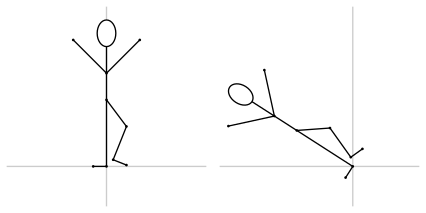
\includegraphics{1_g_dancer_rotate}} 
%\resizebox{!}{1.5in}{\includegraphics{Dancing_man_original}} \hspace{0.5in}  \resizebox{!}{1.5in}{\includegraphics{Dancing_man_rotate}}
\caption{A dancing figure and a rotated dancing figure.}
\label{F:Rotate_dance}
\end{center}
\end{figure}

\csection{Introduction}

In this section we will consider special functions which take vectors as inputs and produce vectors as outputs. We will use matrix multiplication to produce the output vectors.

If $A$ is an $m \times n$ matrix and $\vx$ is a vector in $\R^n$, then the matrix-vector product $A \vx$ is a vector in $\R^m$. (Pick some specific $n, m$ values to understand this statement better.) Therefore, left multiplication by the matrix $A$ takes an input vector $\vx$ in $\R^n$ and produces an output vector $A\vx$ in $\R^m$, which we will refer to as the \emph{image} of $\vx$ under the transformation. This defines a function $T$ from $\R^n$ to $\R^m$ where
\[ T(\vx) = A \vx \, .\]
These functions are the matrix transformations. 

\begin{definition} A \textbf{matrix transformation}\index{matrix transformation}\index{transformation!matrix} is a function $T: \R^n \to \R^m$ defined by 
\[T(\vx) = A\vx\]
for some $m \times n$ matrix $A$. 
\end{definition}

Many of the transformations we consider in this section are from $\R^2$ to $\R^2$ so that we can visualize the transformations.  As an example, let us consider the transformation $T$ defined by 
\[T\left(\left[ \begin{array}{c} x_1 \\ x_2 \end{array} \right] \right) = \left[ \begin{array}{cr} 1&0 \\ 0&-1 \end{array} \right]\left[ \begin{array}{c} x_1 \\ x_2 \end{array} \right]. \]

If we plot the input vectors $\vu_1 = \left[ \begin{array}{c}  1 \\ 0 \end{array} \right]$, $\vu_2 = \left[ \begin{array}{c}  0\\1 \end{array} \right]$, $\vu_3 = \left[ \begin{array}{c} 1  \\ 2 \end{array} \right]$, and  $\vu_4 = \left[ \begin{array}{r} -1  \\ 1 \end{array} \right]$ (as (blue) circles) and their images $T(\vu_1) = \left[ \begin{array}{cr} 1&0 \\ 0&-1 \end{array} \right]\left[ \begin{array}{c} 1 \\ 0 \end{array} \right] = \left[ \begin{array}{c} 1 \\ 0 \end{array} \right]$, $T(\vu_2) = \left[ \begin{array}{r} 0 \\ -1 \end{array} \right]$, $T(\vu_3) = \left[ \begin{array}{r} 1 \\ -2 \end{array} \right]$, and $T(\vu_4) = \left[ \begin{array}{r} -1 \\ -1 \end{array} \right]$ (as (red) $\times$'s) on the same set of axes as shown in Figure \ref{F:PA_1g_1}, we see that this transformation reflects the input vectors across the $x$-axis. We can also see this algebraically since the reflection of the point $(x_1,x_2)$ around the $x$-axis is the point $(x_1,-x_2)$, and 
\[T\left( \left[ \begin{array}{c} x_1 \\ x_2 \end{array} \right] \right) = \left[ \begin{array}{r} x_1 \\ -x_2 \end{array} \right].\]

\begin{figure}[ht]
\begin{center}
\resizebox{!}{3.0in}{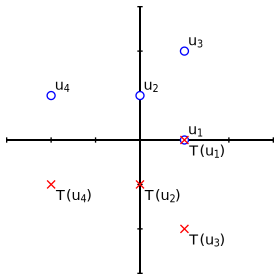
\includegraphics{1g_pa1_b}}
\caption{Inputs and outputs of the transformation $T$.}
\label{F:PA_1g_1}
\end{center}
\end{figure}	

\begin{pa} \label{pa:1_g} We now consider other transformations from $\R^2$ to $\R^2$. 

\be	
\item Suppose a transformation $T$ is defined by 
\[T\left( \left[ \begin{array}{c}  x_1\\x_2 \end{array} \right] \right) = \left[ \begin{array}{cc} 2&0 \\ 0&2 \end{array} \right] \left[ \begin{array}{c}  x_1 \\ x_2 \end{array} \right].\]
	\ba
	\item Find $T(\vu_i)$ for each of $\vu_1 = \left[ \begin{array}{c}  1 \\ 0 \end{array} \right]$, $\vu_2 = \left[ \begin{array}{c}  0\\1 \end{array} \right]$, $\vu_3 = \left[ \begin{array}{c} 1  \\ 2 \end{array} \right]$, and  $\vu_4 = \left[ \begin{array}{r} -1  \\ 1 \end{array} \right]$. (In other words, substitute $\vu_1, \vu_2, \vu_3, \vu_4$ into the formula above to see what output is obtained.)

	\item Plot all input vectors and their images on the same axes in $\R^2$. Clearly identify which image corresponds to which input vector. Then give a geometric description of what this transformation does. 


	\ea
	
\item The transformation in the introduction performs a reflection across the $x$-axis. Find a matrix transformation that performs a reflection across the $y$-axis.

	
\item Suppose a transformation $T$ is defined by 
\[T(\vx) = A\vx,\]
where 
\[A = \left[ \begin{array}{cc} 1&0 \\ 0&0 \end{array} \right].\]
	\ba
	\item Find $T(\vu_i)$ for each of $\vu_1 = \left[ \begin{array}{c}  1 \\ 0 \end{array} \right]$, $\vu_2 = \left[ \begin{array}{c}  0\\1 \end{array} \right]$, $\vu_3 = \left[ \begin{array}{c} 1  \\ 2 \end{array} \right]$, and  $\vu_4 = \left[ \begin{array}{r} -1  \\ 1 \end{array} \right]$. 


	\item Plot all input vectors and their images on the same axes in $\R^2$. Give a geometric description of this transformation.

	\item Is there an input vector which produces $\vb = \left[ \begin{array}{c}  1 \\ 1 \end{array} \right]$ as an output vector?


	\item Find all input vectors that produce the output vector $\vb = \left[ \begin{array}{c}  1 \\ 0 \end{array} \right]$. Is there a unique input vector, or multiple input vectors? 

	\ea
	

\ee
\end{pa}


\csection{Properties of Matrix Transformations}

A matrix transformation is a function. When dealing with functions in previous mathematics courses we have used the terms domain and range with our functions. Recall that the domain of a function is the set of all allowable inputs into the function and the range of a function is the set of all outputs of the function. We do the same with transformations. If $T$ is the matrix transformation $T(\vx) = A \vx$ for some $m \times n$ matrix $A$, then $T$ maps vectors from $\R^n$ into $\R^m$. So $\R^n$ is the \emph{domain}\index{domain of a matrix transformation} of $T$ -- the set of all input vectors. However, the set $\R^m$ is only the target set for $T$ and not necessarily the range of $T$.  We call $\R^m$ the \emph{codomain}\index{codomain of a matrix transformation}  of $T$, while the \emph{range}\index{range of a matrix transformation} of $T$ is the set of all output vectors. The range of a transformation will come up later, so we make a formal definition.

\begin{definition} The \textbf{range}\index{range of a matrix transformation} of a matrix transformation $T$ from $\R^n$ to $\R^m$ is the set 
\[\Range{T} = \{T(\vx) : \vx \in \R^n\}.\]
\end{definition}

The range is always a subset of the codomain, but the two sets do not have to be equal. In addition, if a vector $\vb$ in $\R^m$ satisfies $\vb = T(\vx)$ for some $\vx$ in $\R^n$, then we say that $\vb$ is the \emph{image}\index{image of an element under a transformation} of $\vx$ under the transformation $T$. For this reason we also use the term \emph{image}\index{image of a matrix transformation} to also mean the range of a transformation, with the corresponding notation $\Image(T)$. 



Because of the properties of the matrix-vector product, if the matrix transformation $T$ is defined by $T(\vx) = A\vx$ for some $m \times n$ matrix $A$, then 
\[T(\vu + \vv) =  A(\vu + \vv) = A\vu + A\vv\]
and 
\[T(c\vu) = A(c\vu) = cA\vu = cT(\vu)\]
for any vectors $\vu$ and $\vv$ in $\R^n$ and any scalar $c$. So every matrix transformation $T$ satisfies the following two important properties:
\begin{enumerate}
\item $T(\vu + \vv) =  T(\vu) + T(\vv)$ and
\item $T(c\vu) = c T(\vv)$.
\end{enumerate}
The first property says that a matrix transformation $T$ preserves sums of vectors and the second that $T$ preserves scalar multiples of vectors. 


\begin{activity} \label{act:1_g_2} Let $T$ be a matrix transformation, and let $\vu$ and $\vv$ be vectors in the domain of $T$ so that $T(\vu) = \left[ \begin{array}{c} 1 \\ 2 \\  0 \end{array} \right]$ and $T(\vv) = \left[ \begin{array}{r} -3 \\ 1 \\  4 \end{array} \right]$. 
\ba
\item Exactly which vector is $T(2\vu - 3\vv)$? Explain.

\item If $a$ and $b$ are any scalars, what is the vector $T(a\vu + b\vv)$? Why? 

\ea

\end{activity}


As we saw in Activity \ref{act:1_g_2}, we can combine the two properties of a matrix transformation $T$ into one: for any scalars $a$ and $b$ and any vectors $\vu$ and $\vv$ in the domain of $T$ we have  
\begin{equation} \label{eq:1_g_1}
T(a\vu+b\vv) = aT(\vu) + bT(\vv).
\end{equation}
 We can then extend equation (\ref{eq:1_g_1}) (by mathematical induction) to any finite linear combination of vectors. That is, if $\vv_1$, $\vv_2$, $\ldots$, $\vv_k$ are any vectors in the domain of a matrix transformation $T$ and if $x_1$, $x_2$, $\ldots$, $x_k$ are any scalars, then
\begin{equation} \label{eq:1_g_2}
T(x_1 \vv_1 + x_2 \vv_2 + \cdots + x_k \vv_k) = x_1 T(\vv_1) + x_2 T(\vv_2) + \cdots + x_k T(\vv_k).
\end{equation}
In other words, a matrix transformation preserves linear combinations. For this reason matrix transformations are examples of a larger set of transformation that are called \emph{linear} transformations. We will discuss general linear transformations in a later section.
 

There is one other important property of a matrix transformation for us to consider. The functions we encountered in earlier mathematics courses, e.g., $f(x) = 2x+1$, could send the input 0 to any output. However, as a consequence of the definition, any matrix transformation $T$ maps the zero vector to the zero vector because
\[ T(\vzero) = A\vzero = \vzero \,.\]

Note that the two vectors $\vzero$ in the last equation may not be the same vector -- if $T : \R^n \to \R^m$, then the first $\vzero$ is in $\R^n$ and the second in $\R^m$. It should be clear from the context which vector $\vzero$ is meant. 


\csection{Onto and One-to-One Transformations}

The problems we have been asking about solutions to systems of linear equations can be rephrased in terms of matrix transformations. The question about whether a system $A \vx = \vb$ is consistent for any vector $\vb$ is also a question about the existence of a vector $\vx$ so that $T(\vx) = \vb$, where $T$ is the matrix transformation defined by $T(\vx) = A \vx$. 


\begin{activity} \label{act:1_g_4} Let $T$ be the matrix transformation defined by $T(\vx) = A\vx$ where $A$ is 
\[\left[ \begin{array}{rc} 1&0 \\ 0&1 \\ 0&2 \end{array} \right].\] 
\ba
\item Find $T\left(\left[\begin{array}{c} 1\\1\end{array}\right]\right)$ and $T\left(\left[\begin{array}{c} 1\\1\\1\end{array}\right]\right)$. If it is not possible to find one or both of the output vectors, indicate why.


\item What are the domain and codomain of $T$? Why? (Recall that the domain is the space of all input vectors, while the codomain is the space in which the output vectors are contained.)

\item Can you find a vector $\vx$ for which $T(\vx)= \left[\begin{array}{c} 2\\3\\6\end{array}\right]$? Can you find a vector $\vx$ for which $T(\vx)=\left[\begin{array}{c} 2\\3\\1\end{array}\right]$?

\item Which $\vb=\left[\begin{array}{c} a\\b\\c\end{array}\right]$ are the image vectors for this transformation? Is the range of $T$ equal to the codomain of $T$? Explain. 
 
\item The previous question can be rephrased as a matrix equation question.  We are asking whether $A \vx = \vb$ is consistent for every $\vb$. How is the answer to this question related to the pivots of $A$? 

\ea

\end{activity}


If $T$ is a matrix transformation, Activity \ref{act:1_g_4} illustrates that the range of a matrix transformation $T$ may not equal its codomain. In other words, there may be vectors $\vb$ in the codomain of $T$ that are not the image of any vector in the domain of $T$. If it is the case for a matrix transformation $T$ that there is always a vector $\vx$ in the domain of $T$ such that $T(\vx) = \vb$ for any vector $\vb$ in the codomain of $T$, then $T$ is given a special name.

\begin{definition} A matrix transformation $T$ from $\R^n$ to $\R^m$ is \textbf{onto}\index{onto} if each $\vb$ in $\R^m$ is the image of \emph{at least one} $\vx$ in $\R^n$.
\end{definition}   


So the matrix transformation $T$ from $\R^n$ to $\R^m$ defined by $T(\vx) = A\vx$ is onto if the equation $A \vx = \vb$ has a solution for each vector $\vb$ in $\R^m$. Since the vectors $A\vx$ are linear combinations of the columns of $A$, $T$ is onto exactly when the span of the columns of $A$ is all of $\R^m$. Activity \ref{act:1_g_4} shows us that $T$ is onto if every row of $A$ contains a pivot. 

Another question to ask about matrix transformations is how many vectors there can be that map onto a given output vector.


\begin{activity} \label{act:1_g_5} Let $T$ be the matrix transformation defined by $T(\vx) = A \vx$ where $A$ is 	
\[\left[ \begin{array}{ccc} 1 & 3 & 0 \\ 0 & 0 & 1 \end{array} \right].\]
\ba
\item Find $T\left(\left[\begin{array}{c} 1\\1\end{array}\right]\right)$ and $T\left(\left[\begin{array}{c} 1\\1\\1\end{array}\right]\right)$. If it is not possible to find one or both of the output vectors, indicate why.


\item What are the domain and codomain of $T$? Why?


\item Find $T\left(\left[\begin{array}{c} 1\\1\\2\end{array}\right]\right)$. Are there any other $\vx$'s for which $T(\vx)$ is this same output vector? (Hint: Set up an equation to solve for such $\vx$'s.)
  
\item Assume more generally that for some vector $\vb$, there is a vector $\vx$ so that $T(\vx) = \vb$. Write this as a matrix equation to determine how many solutions this equation has. Explain. How is the answer to this question related to the pivots of $A$?

\ea

\end{activity}


The uniqueness of a solution to $A \vx = \vb$ is the same as saying that the matrix transformation $T$ defined by $T(\vx) = A\vx$ maps exactly one vector to $\vb$. A matrix transformation $T$ that has the property that every image vector is an image in exactly one way is also a special type of transformation.


\begin{definition} A matrix transformation $T$ from $\R^n$ to $\R^m$ is \textbf{one-to-one}\index{one-to-one} if each $\vb$ in $\R^m$ is the image of \emph{at most} one $\vx$ in $\R^n$.
\end{definition}


So the matrix transformation $T$ from $\R^n$ to $\R^m$ defined by $T(\vx) = A\vx$ is one-to-one if the equation $A \vx = \vb$ has a unique solution whenever $A \vx = \vb$ is consistent. Since the vectors $A\vx$ are linear combinations of the columns of $A$, the unique solution requirement indicates that any output vector can be written in exactly one way as a linear combination of the columns of $A$. This implies that the columns of $A$ are linearly independent. Activity \ref{act:1_g_5} indicates that this happens when every column of $A$ is a pivot column. 


To summarize, if $T$ is a matrix transformation defined by $T(\vx) = A \vx$, then $T$ is onto if every row of $A$ contains a pivot, and $T$ is one-to-one if every column of $A$ is a pivot column. It is important to note the difference: being one-to-one depends on the rows of $A$ and being onto depends on the columns of $A$. 


Having a matrix transformation from $\R^n$ to $\R^m$ can tell us things about $m$ and $n$. For example, when a matrix transformation from $\R^n$ to $\R^m$ is one-to-one, it means that there is a unique input vector for every output vector. Since a matrix transformation preserves the algebraic structure of $\R^n$, this implies that the collection of the images of the vectors in the domain of $T$ form a copy of $\R^n$ inside of $\R^m$. If we think of $T$ as a one-to-one matrix transformation with $T(\vx) = A \vx$ for some $m \times n$ matrix, then every column of $A$ will have to be a pivot column. It follows that if there is a one-to-one matrix transformation from $\R^n$ to $\R^m$, we must have $m \geq n$. Similarly, if a matrix transformation $T$ from $\R^n$ to $\R^m$ is onto, then for each $\vb$ in $\R^m$, if we select one vector in the domain of $T$ whose image is $\vb$, then the collection of these vectors in the domain of $T$ is a copy of $\R^m$ inside of $\R^n$. So if there is an onto matrix transformation from $\R^n$ to $\R^m$, then $n \geq m$. As a consequence, the only way a matrix transformation from $\R^n$ to $\R^m$ is both one-to-one and onto is if $n = m$. 

We conclude this section by adding new equivalent conditions to Theorems \ref{thm:IMT_1_e}  and \ref{thm:IMT_1_f} from Sections \ref{sec:matrix_vector} and \ref{sec:independence}.

\begin{theorem} \label{thm:IMT_1_g_a}Let $A$ be an $m \times n$ matrix. The following statements are equivalent.
    \begin{enumerate}
    \item The matrix equation $A \vx = \vb$ has a solution for every vector $\vb$ in $\R^m$.
    \item Every vector $\vb$ in $\R^m$ can be written as a linear combination of the columns of $A$.
    \item The span of the columns of $A$ is $\R^m$.
    \item The matrix $A$ has a pivot position in each row.
    \item The matrix transformation $T$ from $\R^n$ to $\R^m$ defined by $T(\vx) = A\vx$ is onto.
    \end{enumerate}
\end{theorem}


\begin{theorem} \label{thm:IMT_1_g_b} Let $A$ be an $m \times n$ matrix. The following statements are equivalent.
    \begin{enumerate}
    \item The matrix equation $A \vx = \vb$ has a unique solution for every vector $\vb$ in the span of the columns of $A$.
    \item The matrix equation $A \vx = \vzero$ has the unique solution $\vx = \vzero$.
    \item The columns of $A$ are linearly independent.
    \item The matrix $A$ has a pivot position in each column. 
    \item The matrix transformation $T$ from $\R^n$ to $\R^m$ defined by $T(\vx) = A\vx$ is one-to-one.
    \end{enumerate}
\end{theorem}


We will continue to add to these theorems, which will eventually give us many different but equivalent perspectives to look at a linear algebra problem. Please keep these equivalent criteria in mind when considering the best possible approach to a problem.

\csection{Examples}

\ExampleIntro

\begin{example} Let $A = \left[ \begin{array}{crrr} 1&1&-1&-1 \\ 3&6&0&3 \\ 2&-1&-5&-8 \end{array} \right]$ and let $T(\vx) = A\vx$. 
	\ba
	\item Identify the domain of $T$. Explain your reasoning.
	
	\item Is $T$ one-to-one. Explain.
	
	\item Is $T$ onto? If yes, explain why. If no, describe the range of $T$ as best you can, both algebraically and graphically. 
	
	\ea

\ExampleSolution	
\ba
\item Since $A$ is a $3 \times 4$ matrix, $A$ has four columns. Now $A \vx$ is a linear combination of the columns of $A$ with weights from $\vx$, so $\vx$ must have four entries to correspond to the columns of $A$. We conclude that the domain of $T$ is $\R^4$. 

\item Technology shows that the reduced row echelon form of $A$ is 
\[\left[ \begin{array}{ccrr} 1&0&-2&-3 \\ 0&1&1&2 \\ 0&0&0&0 \end{array} \right].\]
Since $A$ contains non-pivot columns, the homogeneous system $A \vx = \vzero$ has infinitely many solutions. So $T$ is not one-to-one. In other words, if there is a column of $A$ that is a non-pivot column, then $A$ is not one-to-one.
	
\item Since the reduced row echelon form of $A$ has rows of zeros, there will be vectors $\vb$ in $\R^3$ such that the reduced row echelon form of $[A \ \vb]$ will have a row of the form $[0 \ 0  \ 0 \ 0 \ c]$ for some nonzero scalar $c$. This means that $T(\vx) = A\vx = \vb$ will have no solution and $T$ is not onto. In other words, if there is a row of $A$ that does not contain a pivot, then $T$ is not onto. 

\item To determine the vectors $\vb = \left[ \begin{array}{c} r\\s\\t \end{array} \right]$ so that $T(\vx) = A\vx = \vb$ is consistent, we row reduce the augmented matrix $[A \ | \  \vb]$. Technology shows that an echelon form of $[A \ \vb]$ is 
\[\left[ \begin{array}{ccrr|c} 1&1&-1&-1&r \\ 0&3&3&6&s-3r \\ 0&0&0&0&t-5r+s \end{array} \right].\]
Thus, the system $A \vx = \vb$ is consistent if and only if $- 5r+s+t = 0$. We can then write the general output vector to this system as 
\[\vb = \left[ \begin{array}{c} r\\s\\5r-s \end{array} \right] = r\left[ \begin{array}{c} 1\\0\\5\end{array} \right] + s\left[ \begin{array}{r} 0\\1\\-1 \end{array} \right],\]
with $r$ and $s$ any scalars. Since there are two free variables, the vectors $\vb$ in $\R^3$ define a plane through the origin. Letting $r=0$ and $s=1$ and $r=1$ and $s=0$, we see that two points that lie on this plane are $(0,1,-1)$ and $(1,0,5)$. So the range of $T$ is the plane through the origin and the points $(0,1,-1)$ and $(1,0,5)$.

\ea

	

\end{example}

\begin{example} A matrix transformation $T: \R^2 \to \R^2$ defined by 
\[T\left(\left[ \begin{array}{c} x\\y \end{array} \right] \right) = \left[ \begin{array}{c} cx\\y \end{array} \right]\]
is a contraction in the $x$ direction if $0 < c < 1$ and a dilation in the $x$ direction if $c>1$.
	\ba
	\item Find a matrix $A$ such that $T(\vx) = A\vx$. 
	
	\item Sketch the square $S$ with vertices $\vu_1 =  \left[ \begin{array}{c} 0\\0 \end{array} \right]$, $\vu_2 =  \left[ \begin{array}{c} 1\\0 \end{array} \right]$, $\vu_3 =  \left[ \begin{array}{c} 1\\1 \end{array} \right]$, and $\vu_4 =  \left[ \begin{array}{c} 0\\1 \end{array} \right]$. Determine and sketch the image of $S$ under $T$ if $c = 2$. 
	
	\ea
	
\ExampleSolution
\ba
\item Since 
\[\left[ \begin{array}{cc} c&0\\0&1 \end{array}\right] \left[ \begin{array}{c} x\\y \end{array} \right] = 
\left[ \begin{array}{c} cx\\y \end{array} \right],\]
the matrix $A = \left[ \begin{array}{cc} c&0\\0&1 \end{array}\right]$ has the property that $T(\vx) = A\vx$. 

\item We can determine the image of $S$ under $T$ by calculating what $T$ does to the vertices of $S$. Notice that 
\begin{align*}
T(\vu_1) &= \left[ \begin{array}{cc} 2&0\\0&1 \end{array}\right] \left[ \begin{array}{c} 0\\0 \end{array} \right] = \left[ \begin{array}{c} 0\\0 \end{array} \right] \\
T(\vu_2) &= \left[ \begin{array}{cc} 2&0\\0&1 \end{array}\right] \left[ \begin{array}{c} 1\\0 \end{array} \right] = \left[ \begin{array}{c} 2\\0 \end{array} \right] \\
T(\vu_3) &= \left[ \begin{array}{cc} 2&0\\0&1 \end{array}\right] \left[ \begin{array}{c} 1\\1 \end{array} \right] = \left[ \begin{array}{c} 2\\1 \end{array} \right] \\
T(\vu_4) &= \left[ \begin{array}{cc} 2&0\\0&1 \end{array}\right] \left[ \begin{array}{c} 0\\1 \end{array} \right] = \left[ \begin{array}{c} 0\\1 \end{array} \right] 
\end{align*}
Since $T$ is a linear map, the image of $S$ under $T$ is the polygon with vertices $(0,0)$, $(1,0)$, $(2,1)$, and $(0,1)$ as shown in Figure \ref{F:ex:1_g_polygons}.
From Figure \ref{F:ex:1_g_polygons} we can see that $T$ stretches the figure in the $x$ direction only by a factor of 2. 

	\ea
\begin{figure}[ht]
\begin{center}
\resizebox{!}{1.75in}{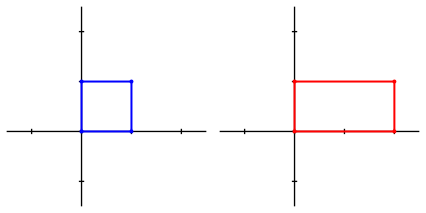
\includegraphics{1_g_polygons}}
\caption{The input square $S$ and the output $T(S)$.}
\label{F:ex:1_g_polygons}
\end{center}
\end{figure}






\end{example}

\csection{Summary}

In this section we determined how to represent any matrix transformation from $\R^n$ to $\R^m$ as a matrix transformation, and what it means for a matrix transformation to be one-to-one and onto.
\begin{itemize}
\item A matrix transformation is a function $T: \R^n \to \R^m$ defined by $T(\vx) = A\vx$ for some $m \times n$ matrix $A$. 
\item A matrix transformation $T$ from $\R^n$ to $\R^m$ satisfies 
\[T(a\vu + b\vv) = aT(\vu) + bT(\vv)\]
for any scalars $a$ and $b$ and any vectors $\vu$ and $\vv$ in $\R^n$. The fact that $T$ preserves linear combinations is why we say that $T$ is a linear transformation. 
\item An $m \times n$ matrix $A$ defines the matrix transformation $T$ via 
\[T(\vx) = A \vx.\]
The domain of this transformation is $\R^n$ because the matrix-vector product $A \vx$ is only defined if $\vx$ is an $n \times 1$ vector. 
\item If $A$ is an $m \times n$ matrix, then the codomain of the matrix transformation $T$ defined by $T(\vx) = A \vx$ is $\R^m$. This is because the matrix-vector product $A \vx$ with $\vx$ an $n \times 1$ vector is an $m \times 1$ vector. The range of $T$ is the subset of the codomain of $T$ consisting of all vectors of the form $T(\vx)$ for vectors $\vx$ in the domain of $T$.
\item A matrix transformation $T$ from $\R^n$ to $\R^m$ is \textbf{one-to-one} if each $\vb$ in $\R^m$ is the image of \emph{at most} one $\vx$ in $\R^n$. If $T$ is a matrix transformation represented as $T(\vx) = A\vx$, then $T$ is one-to-one if each column of $A$ is a pivot column, or if the columns of $A$ are linearly independent.  
\item A matrix transformation $T$ from $\R^n$ to $\R^m$ is \textbf{onto} if each $\vb$ in $\R^m$ is the image of \emph{at least one} $\vx$ in $\R^n$. If $T$ is a matrix transformation represented as $T(\vx) = A\vx$, then $T$ is onto if each row of $A$ contains a pivot position, or if the span of the columns of $A$ is all of $\R^m$.
\end{itemize}




\csection{Exercises}

\be 
\item Given matrix $A=\left[ \begin{array}{ccr} 1& 2 & 1 \\ 1 & 0 & -3 \end{array} \right]$, write the coordinate form of the transformation $T$ defined by $T(\vx)=A\vx$. (Note: Writing a transformation in coordinate form refers to writing the transformation in terms of the entries of the input and output vectors.)

\item Suppose the transformation $T$ is defined by $T(\vx)=A\vx$ where 
\[A=\left[ \begin{array}{ccr} 1&1&-1 \\ 2&1&1 \\ 4&1&4 \end{array} \right].\] Determine if $\vb=\left[ \begin{array}{c} 1\\0\\0 \end{array} \right]$ is in the range of $T$. If so, find all $\vx$'s which map to $\vb$.

\item Suppose $T$ is a matrix transformation and 
\[ T(\vv_1) = \left[ \begin{array}{c} 1 \\ 2 \end{array} \right] \, , \, T(\vv_2) = \left[ \begin{array}{r} -2 \\ 3 \end{array} \right] \]
Find $T(2\vv_1 -5 \vv_2)$.

\item Given a matrix transformation defined as 
\[ T\left( \left[ \begin{array}{c} x_1 \\ x_2 \\ x_3 \end{array} \right] \right) = \left[ \begin{array}{c} 2x_1 -x_3 \\ -x_1 +2x_2 +x_3 \\ 3x_2 - 4x_3 \end{array} \right] \]
determine the matrix $A$ for which $T(\vx) = A\vx$.

\item Suppose a matrix transformation $T$ defined by $T(\vx)=A\vx$ for some unknown $A$ matrix satisfies 
\[ T\left( \left[ \begin{array}{c} 1 \\ 0 \end{array} \right] \right) = \left[ \begin{array}{c} 2\\ 1\end{array} \right] \, \text{ and } \, T\left( \left[ \begin{array}{c} 0 \\ 1 \end{array} \right] \right) = \left[ \begin{array}{r} -1\\ 3\end{array} \right] \, . \] 
Use the matrix transformation properties to determine $T(\vx)$ where $\vx= \left[ \begin{array}{c} x_1\\x_2 \end{array} \right]$. Use the expression for $T(\vx)$ to determine the matrix $A$.

\item For each of the following matrices, determine if the transformation $T$ defined by $T(\vx)=A\vx$ is onto and if $T$ is one-to-one.

\ba
\item $A=\left[ \begin{array}{ccr} 1& 1 & 1 \\ 1 & 2 & -3 \end{array} \right]$

\item $A=\left[ \begin{array}{ccc} 1& 1 & 2 \\ 2 & 2 & 4 \end{array} \right]$

\item $A=\left[ \begin{array}{rcc} 1& 1 & 2 \\ 1 & 2 & 3 \\ -1 & 1 &2 \end{array} \right]$

\item $A=\left[ \begin{array}{cc} 1& 1 \\ 2 & 3 \\ 3 & 0 \end{array} \right]$
\ea

\item Come up with an example of a one-to-one transformation from $\R^3$ to $\R^4$, if possible. If not, explain why not.

\item Come up with an example of an onto transformation from $\R^3$ to $\R^4$, if possible. If not, explain why not.

\item Come up with an example of a one-to-one but not onto transformation from $\R^4$ to $\R^4$, if possible. If not, explain why not.

\item Two students are talking about when a matrix transformation is one-to-one.
\begin{quote}
Student 1: If we have a matrix transformation, then we need to check that $A\vx=\vb$ has a unique solution for every $\vb$ for which $A\vx=\vb$ has a solution, right?
\end{quote} 
\begin{quote}
Student 2: Well, that's the definition. Each $\vb$ in the codomain has to be the image of at most one $\vx$ in the domain. So when $\vb$ is in the range, corresponding to $A\vx=\vb$ having a solution, then there is exactly one solution $\vx$.
\end{quote} 
\begin{quote}
Student 1: But wouldn't it be enough to check that $A\vx=\vzero$ has a unique solution? Doesn't that translate to the other $\vb$ vectors? If there is a unique solution for one $\vb_1$, then there can't be infinitely many solutions for another $\vb_2$.
\end{quote} 
\begin{quote}
Student 2: I don't know. It feels to me as if changing the right hand side could change whether there is a unique solution, or infinitely many solutions, or no solution.
\end{quote}
Which part of the above conversation do you agree with? Which parts need fixing? 

\item Show that if $T$ is a matrix transformation from $\R^n$ to $\R^m$ and $L$ is a line in $\R^n$, then $T(L)$, the image of $L$, is a line or a single vector. (Note that a line in $\R^n$ is the set of all vectors of the form $\vv+c\vw$ where $c$ is a scalar, and $\vv, \vw$ are two fixed vectors in $\R^n$.) 

\item Label each of the following statements as True or False. Provide justification for your response.
\ba
\item \textbf{True/False} The range of a transformation is the same as the codomain of the transformation.

\item \textbf{True/False} The codomain of a transformation $T$ defined by $T(\vx)=A\vx$ is the span of the columns of $A$.

\item \textbf{True/False} A one-to-one transformation is a transformation where each input has a unique output.

\item \textbf{True/False} A one-to-one transformation is a transformation where each output can only come from a unique input.

\item \textbf{True/False} If a matrix transformation from $\R^n$ to $\R^n$ is one-to-one, then it is also onto.

\item \textbf{True/False} A matrix transformation from $\R^2$ to $\R^3$ cannot be onto.

\item \textbf{True/False} A matrix transformation from $\R^3$ to $\R^2$ cannot be onto.

\item \textbf{True/False} A matrix transformation from $\R^3$ to $\R^2$ cannot be one-to-one.

\item \textbf{True/False} If the columns of a matrix $A$ are linearly independent, then the transformation $T$ defined by $T(\vx)=A\vx$ is onto.

\item \textbf{True/False} If the columns of a matrix $A$ are linearly independent, then the transformation $T$ defined by $T(\vx)=A\vx$ is one-to-one.

\item \textbf{True/False} If $A$ is an $m \times n$ matrix with $n$ pivots, then the transformation $\vx \mapsto A\vx$ is onto.

\item \textbf{True/False} If $A$ is an $m \times n$ matrix with $n$ pivots, then the transformation $\vx \mapsto A\vx$ is one-to-one.

\item \textbf{True/False} If $\vu$ is in the range of a matrix transformation $T$, then there is an $\vx$ in the domain of $T$ such that $T(\vx)=\vu$.

\item \textbf{True/False} If $T$ is a one-to-one matrix transformation, then $T(\vx)=\vzero$ has a non-trivial solution.

\item \textbf{True/False} If the transformations $T_1: \R^m \to \R^n$ and $T_2:\R^n \to \R^p$ are onto, then the transformation $T_2 \circ T_1$ defined by $T_2\circ T_1(\vx)=T_2(T_1(\vx))$ is also onto.

\item \textbf{True/False} If the transformations $T_1: \R^m \to \R^n$ and $T_2:\R^n \to \R^p$ are one-to-one, then the transformation $T_2 \circ T_1$ defined by $T_2\circ T_1(\vx)=T_2(T_1(\vx))$ is also one-to-one.

\ea
\ee

\csection{Project: The Geometry of Matrix Transformations}

In this section we will consider certain types of matrix transformations and analyze their geometry. Much more would be needed for real computer graphics, but the essential ideas are contained in our examples. A GeoGebra applet is available at \url{https://www.geogebra.org/m/rh4bzxee} for you to use to visualize the transformations in this project. 

\begin{pactivity} \label{act:1_g_rotation} We begin with transformations that produce the rotated dancing image in Figure \ref{F:Rotate_dance}. Let $R$ be the matrix transformation from $\R^2$ to $\R^2$ defined by 
\[R\left(\left[ \begin{array}{c} x \\ y \end{array} \right] \right) = \left[\begin{array}{lr} \cos(\theta) & -\sin(\theta) \\ \sin(\theta) & \cos(\theta) \end{array} \right]\left[ \begin{array}{c} x \\ y \end{array} \right]. \]
These matrices are the rotation matrices.\index{rotation matrix}
	\ba
	\item Suppose $\theta = \frac{\pi}{2}$. Then 
\[R\left(\left[ \begin{array}{c} x \\ y \end{array} \right] \right) = \left[ \begin{array}{cr} 0&-1 \\ 1&0 \end{array} \right] \left[ \begin{array}{c} x \\ y \end{array} \right]. \]
		\begin{enumerate}[i.]
		\item Find the images of $\vu_1 = \left[ \begin{array}{c} 1 \\ 0 \end{array} \right]$,  $\vu_2 = \left[ \renewcommand{\arraystretch}{1.4} \begin{array}{c} \frac{\sqrt{2}}{2} \\ \frac{\sqrt{2}}{2}  \end{array} \right]$, and $\vu_3 = \left[ \begin{array}{c} 0 \\ 1 \end{array} \right]$ under $R$.

		\item Plot the points determined by the vectors from part i. The matrix transformation $R$ performs a rotation. Based on this small amount of data, what would you say the angle of rotation is for this transformation $R$? 

		\end{enumerate}
	
	\item Now let $R$ be the general matrix transformation defined by the matrix \[\left[\begin{array}{lr} \cos(\theta) & -\sin(\theta) \\ \sin(\theta) & \cos(\theta) \end{array} \right].\] Follow the steps indicated to show that $R$ performs a counterclockwise rotation of an angle $\theta$ around the origin. Let $P$ be the point defined by the vector $\left[ \begin{array}{c} x\\y \end{array} \right] = \left[ \begin{array}{c}\cos(\alpha) \\ \sin(\alpha) \end{array} \right]$ and $Q$ the point defined by the vector $\left[ \begin{array}{c} w\\z \end{array} \right] = \left[ \begin{array}{c} \cos(\alpha+\theta) \\ \sin(\alpha+\theta) \end{array} \right]$ as illustrated in Figure \ref{fig:Rotation_matrix}.
\begin{figure}[h]
\begin{center}
\resizebox{!}{2.0in}{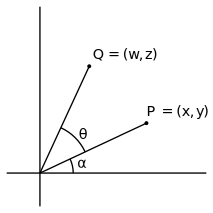
\includegraphics{Rotation_matrix}}
\caption{A rotation in the plane.}
\label{fig:Rotation_matrix}
\end{center}
\end{figure}
		\begin{enumerate}[i.]
		        \item Use the angle sum trigonometric identities 
		        \begin{align*}
		        \cos(A+B) &= \cos(A) \cos(B) - \sin(A) \sin(B) \\
		         \sin(A+B) &= \cos(A) \sin(B) + \cos(B) \sin(A)
		        \end{align*}
		        to show that
    \begin{align*}
    w &= \cos(\theta)x - \sin(\theta)y \\
    z &=  \sin(\theta)x + \cos(\theta)y.
    \end{align*}

	\item Now explain why the counterclockwise rotation around the origin by an angle $\theta$ can be represented by left multiplication by the matrix 
            \[\left[ \begin{array}{rr} \cos(\theta) & -\sin(\theta) \\ \sin(\theta) & \cos(\theta) \end{array} \right].\]
        
	\end{enumerate}
		
	\ea
	
\end{pactivity}

Project Activity \ref{act:1_g_rotation} presented the rotation matrices. Other matrices have different effects. 

\begin{pactivity} \label{act:1_g_shear} Different matrix transformations 
\ba
\item Let $S$ be the matrix transformation from $\R^2$ to $\R^2$ defined by 
\[S\left(\left[ \begin{array}{c} x \\ y \end{array} \right] \right) = \left[ \begin{array}{cr} 1&0.5 \\ 0&1 \end{array} \right]\left[ \begin{array}{c} x \\ y \end{array} \right].\]

Determine the entries of the output vector $S\left(\left[ \begin{array}{c} x \\ y \end{array} \right] \right)$ and explain the action of the transformation $S$ on the dancing figure as illustrated in Figure \ref{F:Shear_x_Dance}. (The transformation $S$ is called a \emph{shear}\index{shear} in the $x$ direction.)
\begin{figure}[ht]
\begin{center}
\resizebox{!}{1.5in}{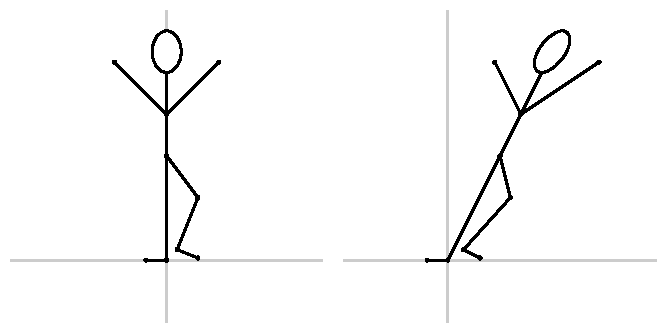
\includegraphics{1_g_shear_x}} 
%\resizebox{!}{1.5in}{\includegraphics{Dancing_man_original}} \hspace{0.5in}  \resizebox{!}{1.5in}{\includegraphics{Dancing_man_shear_x}}
\caption{A dancing figure and a sheared dancing figure.}
\label{F:Shear_x_Dance}
\end{center}
\end{figure}
%\resizebox{!}{1.0in}{\includegraphics{1g_dancing_man_shearx}}


\item Let $C$ be the matrix transformation from $\R^2$ to $\R^2$ defined by 
\[C\left(\left[ \begin{array}{c} x \\ y \end{array} \right] \right) = \left[ \begin{array}{cr} 0.65&0 \\ 0&0.65 \end{array} \right]\left[ \begin{array}{c} x \\ y \end{array} \right].\]

Determine the entries of the output vector $C\left(\left[ \begin{array}{c} x \\ y \end{array} \right] \right)$ and explain the action of the transformation $C$ on the dancing figure as illustrated in Figure \ref{F:Contract_Dance}. (The transformation $C$ is called a \emph{contraction}\index{contraction}.) How would your response change if each $0.65$ was changed to $2$ in the matrix $C$? 
\begin{figure}[ht]
\begin{center}
\resizebox{!}{1.0in}{\includegraphics{1_g_dancer_contract}}
%\resizebox{!}{1.5in}{\includegraphics{Dancing_man_original}} \hspace{0.5in}  \resizebox{!}{1.5in}{\includegraphics{Dancing_man_scale}}
\caption{A dancing figure and a contracted dancing figure.}
\label{F:Contract_Dance}
\end{center}
\end{figure} 

\ea

\end{pactivity}

So far we have seen specific matrix transformations perform a rotations, shears, and contractions. We can combine these, and other, matrix transformations by composition to change figures in different ways, and to created animations of geometric figures. (As we will see later, combining transformations needs to be done carefully in order to obtain the result we want. For example, if we want to first rotate then translate, in what order should the matrices be applied?)


  %7

%\end{comment}

%\begin{comment}

\part{Matrices}

\achapter{8}{Matrix Operations} \label{chap:matrix_operations}

\vspace*{-17 pt}
\framebox{
\parbox{\dimexpr\linewidth-3\fboxsep-3\fboxrule}
{\begin{fqs}
\item Under what conditions can we add two matrices and how is the matrix sum defined? 
\item Under what conditions can we multiply a matrix by a scalar and how is a scalar multiple of a matrix defined? 
\item Under what conditions can we multiply two matrices and how is the matrix product defined?
\item What properties do matrix addition, scalar multiplication of matrices and matrix multiplication satisfy? Are these properties similar to properties that are satisfied by vector operations? 
\item What are two properties that make matrix multiplication fundamentally different than our standard product of real numbers? 
\item What is the interpretation of matrix multiplication from the perspective of linear transformations?
\item How is the transpose of a matrix defined? 
\end{fqs}}}% \hspace*{3 pt}}

\vspace*{13 pt}

\csection{Application: Algorithms for Matrix Multiplication}
\label{sec:appl_mtx_mult}

Matrix multiplication is widely used in applications ranging from scientific computing and pattern recognition to counting paths in graphs. As a consequence, much work is being done in developing efficient algorithms for matrix multiplication. 

We will see that a matrix product can be calculated through the row-column method. Recall that the product of two $2 \times 2$ matrices $A = \left[ \begin{array}{cc} a_{11}&a_{12}\\a_{21}&a_{22} \end{array} \right]$ and $B = \left[ \begin{array}{cc} b_{11}&b_{12}\\b_{21}&b_{22} \end{array} \right]$ is given by 
\[AB = \left[ \begin{array}{cc} a_{11}b_{11}+a_{12}b_{21} & a_{11}b_{12}+a_{12}b_{22} \\ a_{21}b_{11}+a_{22}b_{21} & a_{21}b_{12}+a_{22}b_{22} \end{array} \right],\]
This product involves eight scalar multiplications and some scalar additions. As we will see, multiplication is more computationally expensive than addition, so we will focus on multiplication. In 1969, a German mathematician named Volker Strassen showed\footnote{Strassen, Volker, Gaussian Elimination is not Optimal, Number. Math. 13, p. 354-356, 1969} that the product of two $2 \times 2$ matrices can be calculated using only seven multiplications. While this is not much of an improvement, the Strassen algorithm can be applied to larger matrices, using matrix partitions (which allow for parallel computation), and its publication led to additional research on faster algorithms for matrix multiplication. More details are provided later in this section. 



\csection{Introduction}
\label{sec:mtx_ops_intro}

A vector is a list of numbers in a specified order and a matrix is an ordered array of objects. In fact, a vector can be thought of as a matrix of size $n \times 1$. Vectors and matrices are so alike in this way that it would seem natural that we can define operations on matrices just as we did with vectors. 

Recall that a matrix is made of rows and columns -- the entries reading from left to right form the \emph{rows} of the matrix and the entries reading from top to bottom form the \emph{columns}. The number of rows and columns of a matrix is called the \emph{size} of the matrix, so an $m \times n$ matrix has $m$ rows and $n$ columns. If we label the entry in the $i$th row and $j$th column of a matrix $A$ as $a_{ij}$, then we write $A = [a_{ij}]$. 

We can generalize the operations of addition and scalar multiplication on vectors to matrices similarly. Given two matrices $A=[a_{ij}]$ and $B=[b_{ij}]$ of the same size, we define the sum $A+B$ by
\[ A+B= [ a_{ij}+b_{ij} ] \]
when the sizes of the matrices $A$ and $B$ match. In other words, for matrices of the same size the matrix addition is defined by adding corresponding entries in the matrices. For example,
\[ \left[ \begin{array}{rc} 1 & 2 \\ -2 & 3  \end{array} \right] + \left[ \begin{array}{cc} 1 & 3 \\ 2 & 4  \end{array} \right] = \left[ \begin{array}{cc} 2 & 5 \\ 0 & 7  \end{array} \right]  \,.\]

We define the scalar multiple of a matrix $A=[a_{ij}]$ by scalar $c$ to be the matrix $cA$ defined by
\[ cA= [ ca_{ij}] \, .\index{matrix!scalar multiple}\]
This means that we multiply each entry of the matrix $A$ by the scalar $c$. As an example, 
\[ 3 \left[ \begin{array}{rc} 1 & 2 \\ -2 & 3  \end{array} \right] = \left[ \begin{array}{rc} 3 & 6 \\ -6 & 9  \end{array} \right] \,.\]

Even though we did not have a multiplication operation on vectors, we had a matrix-vector product, which is a special case of a matrix-matrix product since a vector is a matrix with one column. However, generalizing the matrix-vector product to a matrix-matrix product is not immediate as it is not immediately clear what we can do with the other columns. We will consider this question in this section.

Note that all of the matrix operations can be performed on a calculator. After entering each matrix in the calculator, just use $+$, $-$ and $\times$ operations to find the result of the matrix operation. (Just for fun, try using $\div$ with matrices to see if it will work.)\\

\begin{pa} \label{pa:2_a} ~
\be
\item Pick three different varying sizes of pairs of $A, B$ matrices which can be added. For each pair:
	\ba
	\item Find the matrices $A+B$ and $B+A$.

	\item How are the two matrices $A+B$ and $B+A$ related? What does this tell us about matrix addition?

	\ea


\item Let $A = \left[ \begin{array}{rc} 1 & 0 \\ -2 & 8  \end{array} \right]$,  $B = \left[ \begin{array}{cc} 1 & 1 \\ 3 & 4  \end{array} \right]$, and  $C = \left[ \begin{array}{cr} 0 & -5 \\ 1 & 6  \end{array} \right]$. Determine the entries of the matrix $A + 2B - 7C$.


\item \label{p:matrix_multiplication} Now we turn to multiplication of matrices. Our first goal is to find out what conditions we need on the sizes of matrices $A$ and $B$ if the matrix-matrix product $AB$ is defined and what the size of the resulting product matrix is. We know the condition and the size of the result in the special case of $B$ being a vector, i.e., a matrix with one column. So our conjectures for the general case should match what we know in the special case.

In each part of this problem, use any appropriate tool (e.g., your calculator, Maple, Mathematica, Wolfram$|$Alpha) to determine the matrix product $AB$, if it exists. If you obtain a product, write it down and explain how its size is related to the sizes of $A$ and $B$. If you receive an error, write down the error and guess why the error occurred and/or what it means. 
	\ba
	\item $A = \left[ \begin{array}{ccc} 1&2&0 \\ 0&1&1 \end{array} \right]  \ \ \ \text{ and } \ \ \ B = \left[ \begin{array}{crc} 3&5&0\\0&-2&1 \end{array} \right]$



	\item $A = \left[ \begin{array}{ccc} 1&2&0 \\ 0&1&1 \end{array} \right]  \ \ \ \text{ and } \ \ \ B = \left[ \begin{array}{crc} 3&0\\5&-2 \\ 0&1 \end{array} \right]$


 \item $A = \left[ \begin{array}{cc} 1 & 2 \\ 3 & 4\end{array} \right]  \ \ \ \text{ and } \ \ \ B = \left[ \begin{array}{ccc}
1 & 1 & 1 \\1 & 0 & 1 \\ 0 & 2 & 0\end{array} \right]$

 \item $A = \left[ \begin{array}{cc} 1 & 2 \\ 3 & 4 \\ 5 & 6 \\ 7 & 8 \end{array} \right]  \ \ \ \text{ and } \ \ \ B = \left[ \begin{array}{rcc} 1 & 2 & 3 \\ -1 & 1 & 1\end{array} \right]$

  \item Make a guess for the condition on the sizes of two matrices $A, B$ for which the product $AB$ is defined. How is the size of the product matrix related to the sizes of $A$ and $B$?


	\ea

\item The final matrix products, when defined, in problem \ref{p:matrix_multiplication} might seem unrelated to the individual matrices at first. In this problem, we will uncover this relationship using our knowledge of the matrix-vector product.

Let $A = \left[ \begin{array}{rr} 3 & -1 \\ -2 & 3 \end{array} \right]$ and $B = \left[ \begin{array}{ccc} 0 & 2 & 1 \\ 1 & 3 & 2\end{array} \right]$. 

\ba
\item Calculate $AB$ using any tool.

\item Using the matrix-vector product, calculate $A \vx$ where $\vx$ is the first column (i.e., calculate $A\begin{bmatrix} 0 \\ 1\end{bmatrix}$), and then the second column of $B$ (i.e., calculate $A\begin{bmatrix} 2 \\ 3\end{bmatrix}$), and then the third column of $B$ (i.e., calculate $A\begin{bmatrix} 1 \\ 2\end{bmatrix}$). Do you notice these output vectors within $AB$?

\item Describe as best you can a definition of $AB$ using the matrix-vector product.

\ea
\ee

\end{pa}



\csection{Properties of Matrix Addition and Multiplication by Scalars}
\label{sec:mtx_add_smult}

Just as we were able to define an algebra of vectors with addition and multiplication by scalars, we can define an algebra of matrices. We will see that the properties of these operations on matrices are immediate generalizations of the properties of the operations on vectors. We will then see how the matrix product arises through the connection of matrices to linear transformations. Finally, we define the transpose of a matrix. The transpose of a matrix will be useful in applications such as graph theory and least-squares fitting of curves, as well as in advanced topics such as inner product spaces and the dual space of a vector space.

We learned in Preview Activity \ref{pa:2_a} that we can add two matrices of the same size together by adding corresponding entries and we can multiply any matrix by a scalar by multiplying each entry of the matrix by that scalar. More generally, if $A = [a_{ij}]$ and $B = [b_{ij}]$ are $m \times n$ matrices and $c$ is any scalar, then  
\[A + B = [a_{ij}+b_{ij}] \ \ \text{ and } \ \ cA = [ca_{ij}].\index{matrix!sum}\]

As we have done each time we have introduced a new operation, we ask what properties the operation has. For example, you determined in Preview Activity \ref{pa:2_a} that addition of matrices is a commutative operation. More specifically, for every two $m\times n$ matrices $A$ and $B$, $A+B=B+A$. We can use similar arguments to verify the following properties of matrix addition and multiplication by scalars. Notice that these properties are very similar to the properties of addition and scalar multiplication of vectors we discussed earlier. This should come as no surprise since the $n$-dimensional vectors are $n\times 1$ matrices. In a strange twist, we will see that matrices themselves can be considered as vectors when we discuss vector spaces in a later section.



\begin{theorem} \label{thm:matrix_sum_properties} Let $A$, $B$, and $C$ be $m \times n$ matrices and let $a$ and $b$ be scalars. Then
\begin{enumerate}
\item $A+B = B+A$ (this property tells us that matrix addition is \emph{commutative})
\item $(A+B) + C = A + (B+C)$ (this property tells us that matrix addition is \emph{associative})
\item The $m \times n$ matrix $0$ whose entries are all 0 has the property that $A + 0 = A$. The matrix $0$ is called the \textbf{zero matrix} (It is generally clear from the context what the size of the 0 matrix is.).
\item  The scalar multiple $(-1)A$ of the matrix $A$ has the property that $(-1)A + A = 0$. The matrix $(-1)A = -A$ is called the \textbf{additive inverse} of the matrix $A$.
\item $(a+b) A = aA + bA$ (this property tells us that \emph{scalar multiplication of matrices distributes over scalar addition})
\item $a(A+B) = aA + aB$ (this property tells us that \emph{scalar multiplication of matrices distributes over matrix addition})
\item $(ab) A = a(bA)$
\item $1A=A$.
\end{enumerate}
\end{theorem}



Later on, we will see that these properties define the set of all $m \times n$ matrices as a \emph{vector space}. These properties just say that, regarding addition and multiplication by scalars, we can manipulate matrices just as we do real numbers. Note, however, we have not yet defined an operation of multiplication on matrices. That is the topic for the next section. 

\csection{A Matrix Product}
\label{sec:mtx_prod}

As we saw in Preview Activity \ref{pa:2_a}, a matrix-matrix product can be found in a way which makes use of and also generalizes the matrix-vector product.



\begin{definition} The \textbf{matrix product}\index{matrix!product} of a $k \times m$ matrix $A$ and an $m \times n$ matrix $B = [\vb_1 \ \vb_2 \ \cdots \ \vb_n]$ with columns $\vb_1$, $\vb_2$, $\ldots$, $\vb_n$ is the $k \times n$ matrix
\[[A\vb_1 \ A\vb_2 \ \cdots \ A\vb_n].\]
\end{definition}



We now consider the motivation behind this definition by thinking about the matrix transformations corresponding to each of the matrices $A, B$ and $AB$.
Recall that left multiplication by an $m \times n$ matrix $B$ defines a transformation $T$ from $\R^n$ to $\R^m$ by $T(\vx)=B\vx$. The domain of $T$ is $\R^n$ because the number of components of $\vx$ have to match the number of entries in each of row of $B$ in order for the matrix-vector product $B\vx$ to be defined. Similarly, a $k \times m$ matrix $A$ defines a transformation $A$ from $\R^m$ to $\R^k$. Since transformations are functions, we can compose them as long as the output vectors of the inside transformation lie in the domain of the outside transformation. Therefore if $T$ is the inside transformation and $S$ is the outside transformation, the composition $S\circ T$ is defined. So a natural question to ask is if we are given
\begin{itemize}
\item a transformation $T$ from $\R^n$ to $\R^m$ where $T(\vx) = B \vx$ for an $m \times n$ matrix $B$ and
\item a transformation $S$ from $\R^m$ to $\R^k$ with $S(\vy) = A \vy$ for some $k \times m$ matrix $A$,
\end{itemize}
is there a matrix that represents the transformation $S \circ T$ defined by $(S\circ T)(\vx)=S(T(\vx))$? We investigate this question in the next activity in the special case of a $2\times 3$ matrix $A$ and a $3\times 2$ matrix $B$.

\begin{activity} \label{act:A2.1_1} In this activity, we look for the meaning of the matrix product from a transformation perspective. Let $S$ and $T$ be matrix transformations defined by 
\[S(\vy) = A \vy \ \ \ \text{ and } \ \ \ T(\vx) = B \vx,\]
where 
\[A = \left[ \begin{array}{ccc} 1&2&0 \\ 0&1&1 \end{array} \right]  \ \ \ \text{ and } \ \ \ B = \left[ \begin{array}{cr} 3&0\\5&-2 \\ 0&1 \end{array} \right].\]
	\ba
	\item What are the domains and codomains of $S$ and $T$? Why is the composite transformation $S \circ T$ defined? What is the domain of $S\circ T$? What is the codomain of $S\circ T$? (Recall that $S \circ T$ is defined by $(S \circ T)(\vx) = S(T(\vx))$, i.e., we substitute the output $T(\vx)$ as the input into the transformation $S$.)



	\item Let $\vx = \left[ \begin{array}{c} x \\ y \end{array} \right]$. Determine the components of $T(\vx)$.
	


	\item Find the components of $S\circ T(\vx)=S(T(\vx))$. 
	


	\item Find a matrix $C$ so that $S(T(\vx)) = C\vx$. 
	


	\item Use the definition of composition of transformations and the definitions of the $S$ and $T$ transformations to explain why it is reasonable to define $AB$ to be the matrix $C$. Does the matrix $C$ agree with the 
\[AB = \left[ \begin{array}{cr} 13 & -4 \\ 5 & -1 \end{array} \right]\]
you found in Preview Activity \ref{pa:2_a} using technology?
	


	\ea
\end{activity}



We now consider this result in the general case of a $k\times m$ matrix $A$ and an $m \times n$ matrix $B$, where $A$ and $B$ define matrix transformations $S$ and $T$, respectively. In other words, $S$ and $T$ are matrix transformations defined by $S(\vx) = A\vx$ and $T(\vx) = B\vx$. The domain of $S$ is $\R^m$ and the codomain is $\R^k$. The domain of $T$ is $\R^n$ and the codomain is $\R^m$. The composition $S\circ T$ is defined because the output vectors of $T$ are in $\R^m$ and they lie in the domain of $S$. The domain of $S\circ T$ is the same as the domain of $T$ since the input vectors first go through the $T$ transformation. The codomain of $S\circ T$ is the same as the codomain of $S$ since the final output vectors are produced by applying the $S$ transformation.

Let us see how we can obtain the matrix corresponding to the transformation $S\circ T$. Let $B = \left[ \vb_1 \ \vb_2  \  \cdots \ \vb_n  \right]$, where $\vb_j$ is the $j$th column of $B$, and let $\vx = \left[ \begin{array}{c} x_1 \\ x_2 \\ \vdots \\ x_n \end{array} \right]$. Recall that the matrix vector product $B\vx$ is the linear combination of the columns of $B$ with the corresponding weights from $\vx$. So
\[T(\vx) = B\vx = x_1 \vb_1 + x_2 \vb_2 + \cdots + x_n \vb_n.\]
Note that each of the $\vb_j$ vectors are in $\R^m$ since $B$ is an $m\times n$ matrix. Therefore, each of these vectors can be multiplied by matrix $A$ and we can evaluate $S(B\vx)$. Therefore, $S\circ T$ is defined and 
\begin{equation} 
(S \circ T)(\vx) = S(T(\vx))= A(B\vx) = A\left( x_1 \vb_1 + x_2 \vb_2 + \cdots + x_n \vb_n\right). \label{eq:2_a_1}
\end{equation}
The properties of matrix-vector products show that
\begin{equation} 
A\left( x_1 \vb_1 + x_2 \vb_2 + \cdots + x_n \vb_n\right) = x_1 A\vb_1 + x_2 A\vb_2 + \cdots + x_n A\vb_n. \label{eq:2_a_2}
\end{equation}
This expression is a linear combination of $A\vb_i$'s with $x_i$'s being the weights. Therefore, if we let $C$ be the matrix with columns $A \vb_1$, $A\vb_2$, $\ldots$, $A\vb_n$, that is
\[C = [A \vb_1 \ A\vb_2 \ \cdots \ A\vb_n],\]
then 
\begin{equation}
x_1 A\vb_1 + x_2 A\vb_2 + \cdots + x_n A\vb_n = C \vx \label{eq:2_a_3}
\end{equation}
by definition of the matrix-vector product. Combining equations (\ref{eq:2_a_1}), (\ref{eq:2_a_2}), and (\ref{eq:2_a_3}) shows that
\[(S \circ T)(\vx) = C \vx\]
where $C = [A \vb_1 \ A\vb_2 \ \cdots \ A\vb_n]$. 

Also note that since $T(\vx)=B\vx$ and $S(\vy)=A\vy$, we find 
\begin{equation} 
(S\circ T)(\vx)= S(T(\vx))= S(B\vx)=A(B(\vx)) \,.  \label{eq:2_a_4}
\end{equation}
Since the matrix representing the transformation $S\circ T$ is the matrix 
\[[A \vb_1 \ A\vb_2 \ \cdots \ A\vb_n]\]
where $\vb_1$, $\vb_2$, $\ldots$, $\vb_n$ are the columns of the matrix $B$, it is natural to define $AB$ to be this matrix in light of equation \eqref{eq:2_a_4}.



Matrix multiplication has some properties that are unfamiliar to us as the next activity illustrates.



\begin{activity} \label{act:A2.1_2} Let $A~=~\left[ \begin{array}{rr} 3 & -1 \\ -2 & 6 \end{array} \right]$, $B~=~\left[ \begin{array}{cc} 0 & 2 \\ 1 & 3  \end{array} \right]$, $C~=~\left[ \begin{array}{cc} 1 & 1 \\ 1 & 1 \end{array} \right]$, $D~=~\left[ \begin{array}{rr} 3 & -3 \\ -3 & 3 \end{array} \right]$ and $E~=~\left[ \begin{array}{cc} 1 & 0 \\ 0 & 1 \end{array} \right]$. 
	\ba
	\item Find the indicated products (by hand or using a calculator).\\
		$AB$ \hspace{0.75cm} $BA$ \hspace{0.75cm} $DC$ \hspace{0.75cm} $AC$ \hspace{0.75cm} $BC$ \hspace{0.75cm} $AE$ \hspace{0.75cm} $EB$

   

   
		
	\item Is matrix multiplication commutative? Explain.
	


\item Is there an identity element for matrix multiplication? In other words, is there a matrix $I$ for which $AI=IA=A$ for any matrix $A$? Explain.


    
	\item If $a$ and $b$ are real numbers with $ab=0$, then we know that either $a=0$ or $b=0$. Is this same property true with matrix multiplication? Explain. 
	


	\item If $a$, $b$, and $c$ are real numbers with $c \neq 0$ and $ac = bc$, we know that $a=b$. Is this same property true with matrix multiplication?  Explain.
	
	
	
	
    \ea
\end{activity}



As we saw in Activity \ref{act:A2.1_2}, there are matrices $A, B$ for which $AB\neq BA$. On the other hand, there are matrices for which $AB=BA$. For example, this equality will always hold for a square matrix $A$ and if $B$ is the identity matrix of the same size. It also holds if $A=B$. If the equality $AB=BA$ holds, we say that matrices $A$ and $B$ \emph{commute}. So the identity matrix commutes with all square matrices of the same size and every matrix $A$ commutes with $A^k$ for any power $k$.



There is an alternative method of calculating a matrix product that we will often use that we illustrate in the next activity. This alternate version depends on the product of a row matrix with a vector. Suppose $A = [a_1 \ a_2 \ \cdots \ a_n]$ is a $1 \times n$ matrix and $\vx = \left[ \begin{array}{c} x_1 \\ x_2 \\ \vdots \\ x_n \end{array} \right]$ is an $n \times 1$ vector. Then the product $A \vx$ is the $1 \times 1$ vector 
\[[a_1 \ a_2 \ \cdots \ a_n]\left[ \begin{array}{c} x_1 \\ x_2 \\ \vdots \\ x_n \end{array} \right] = [a_1x_1+a_2x_2 + \cdots + a_nx_n].\]
In this situation, we usually identify the $1 \times 1$ matrix with its scalar entry and write 
\begin{equation} \label{eq:2_a_5}
[a_1 \ a_2 \ \cdots \ a_n] \cdot \left[ \begin{array}{c} x_1 \\ x_2 \\ \vdots \\ x_n \end{array} \right] = a_1x_1+a_2x_2 + \cdots + a_nx_n.
\end{equation}
The product $\cdot$ in (\ref{eq:2_a_5}) is called the \emph{scalar} or \emph{dot}\index{dot product} product of $[a_1 \ a_2 \ \cdots \ a_n]$ with $\left[ \begin{array}{c} x_1 \\ x_2 \\ \vdots \\ x_n \end{array} \right]$. 



\begin{activity} \label{act:A2.1_3} Let $A = \left[ \begin{array}{crr} 1&-1&2 \\ 3&0&-4 \\ 2&-5&1 \end{array} \right]$ and $B = \left[ \begin{array}{cr} 4&-2 \\ 6&0 \\ 1&3 \end{array} \right]$. 

Let $\va_i$ be the $i$th row of $A$ and $\vb_j$ the $j$th column of $B$. For example, $\va_1=[ \, 1 \; -1 \; 2 \, ]$ and $\vb_2 = \left[ \begin{array}{r} -2 \\ 0 \\ 3 \end{array} \right]$. 

Calculate the entries of the matrix $C$, where 
\[C = \left[ \begin{array}{cc} \va_1 \cdot \vb_1 & \va_1 \cdot \vb_2 \\ \va_2 \cdot \vb_1 & \va_2 \cdot \vb_2 \\ \va_3 \cdot \vb_1 & \va_3 \cdot \vb_2 \end{array} \right]\,, \]
where $\va_i \cdot \vb_j$ refers to the scalar product of row $i$ of $A$ with column $j$ of $B$.\footnote{Recall from Exercise \ref{ex:1_e_scalar_product} of Section \ref{sec:matrix_vector} that the scalar product $\vu \cdot \vv$ of a $1 \times n$ matrix $\vu = [u_1 \ u_2 \ \ldots \ u_n]$ and an $n \times 1$ vector $\vv=\left[ \begin{array}{c} v_1\\ v_2\\ \vdots \\ v_n \end{array} \right]$ is $\vu \cdot \vv = u_1v_1 + u_2v_2 + u_3v_3 + \cdots + u_nv_n$.} Compare your result with the result of $AB$ calculated via the product of $A$ with the columns of $B$.



\end{activity}





Activity \ref{act:A2.1_3} shows that these is an alternate way to calculate a matrix product. To see how this works in general, let $A = [a_{ij}]$ be a $k \times m$ matrix and $B = [\vb_1 \ \vb_2 \ \cdots \ \vb_n]$ an $m \times n$ matrix. We know that
\[AB = [A\vb_1 \ A\vb_2 \ \cdots \ A\vb_n].\]
Now let $\vr_1$, $\vr_2$, $\ldots$, $\vr_k$ be the rows of $A$ so that $A = \left[ \begin{array}{c} \vr_1 \\ \vr_2 \\ \vdots \\ \vr_k \end{array} \right]$. First we argue that if $\vx = \left[ \begin{array}{c} x_1 \\ x_2 \\ \vdots \\ x_m \end{array} \right]$, then 
\[A \vx = \left[ \begin{array}{c} \vr_1 \cdot \vx \\ \vr_2 \cdot \vx \\ \vdots \\ \vr_k \cdot \vx \end{array} \right].\]
This is the \emph{scalar product} (or \emph{dot product}) definition of the matrix-vector product.

To show that this definition gives the same result as the linear combination definition of matrix-vector product, we first let $A = [\vc_1 \ \vc_2 \ \cdots \ \vc_m]$, where $\vc_1$, $\vc_2$, $\ldots$, $\vc_m$ are the columns of $A$. By our linear combination definition of the matrix-vector product, we obtain 
\begin{align*}
A \vx &= x_1\vc_1 + x_2 \vc_2 + \cdots + x_m \vc_m \\
	&= x_1 \left[ \begin{array}{c} a_{11} \\ a_{21} \\ \vdots \\ a_{k1} \end{array} \right] + x_2 \left[ \begin{array}{c} a_{12} \\ a_{22} \\ \vdots \\ a_{k2} \end{array} \right] + \cdots + x_m \left[ \begin{array}{c} a_{1m} \\ a_{2m} \\ \vdots \\ a_{km} \end{array} \right] \\
	&= \left[ \begin{array}{c} a_{11}x_1+a_{12}x_2+ \cdots + a_{1m}x_m \\ a_{21}x_1+a_{22}x_2+ \cdots + a_{2m}x_m  \\ \vdots \\ a_{k1}x_1+a_{k2}x_2+ \cdots + a_{km}x_m \end{array} \right] \\
	&= \left[ \begin{array}{c} \vr_1 \cdot \vx \\ \vr_2 \cdot \vx \\ \vdots \\ \vr_k \cdot \vx \end{array} \right].
\end{align*}
Therefore, the above work shows that both linear combination and scalar product definitions give the same matrix-vector product.

Applying this to the matrix product $AB$ defined in terms of the matrix-vector product, we see that 
\[A \vb_j = \left[ \begin{array}{c} \vr_1 \cdot \vb_j \\ \vr_2 \cdot \vb_j \\ \vdots \\ \vr_k \cdot \vb_j \end{array} \right].\]
So the $i,j$th entry of the matrix product $AB$ is found by taking the scalar product of the $i$th row of $A$ with the $j$th column of $B$. In other words,
\[(AB)_{ij} = \vr_i \cdot \vb_j\]
where $\vr_i$ is the $i$th row of $A$ and $\vb_j$ is the $j$th column of $B$.

\subsection*{Properties of Matrix Multiplication}

Activity \ref{act:A2.1_2} shows that we must be very careful not to assume that matrix multiplication behaves like multiplication of real numbers. However, matrix multiplication does satisfy some familiar properties. For example, we now have an addition and multiplication of matrices under certain conditions, so we might ask if matrix multiplication distributes over matrix addition. To answer this question we take two \emph{arbitrary} $k \times m$ matrices $A$ and $B$ and an \emph{arbitrary} $m \times n$ matrix $C =  [\vc_1 \ \vc_2 \ \cdots \ \vc_n]$. Then
\begin{align*}
(A+B)C &= [(A+B)\vc_1 \ (A+B)\vc_2 \ \cdots \ (A+B)\vc_n] \\
    &= [A\vc_1+B\vc_1 \ A\vc_2+B\vc_2 \ \cdots \ A\vc_n+B\vc_n] \\
    &= [A\vc_1 \ A\vc_2 \ \cdots \ A\vc_n] + [B\vc_1 \ B\vc_2 \ \cdots \ B\vc_n] \\
    &= AC + BC.
\end{align*}
Similar arguments can be used to show the following properties of matrix multiplication.



\begin{theorem} \label{thm:matrix_product_properties}  Let $A$, $B$, and $C$ be matrices of the appropriate sizes for all sums and products to be defined and let $a$ be a scalar. Then
\begin{enumerate}
\item $(AB)C = A(BC)$  (this property tells us that matrix multiplication is \emph{associative})
\item $(A+B)C = AC + BC$ (this property tells us that matrix multiplication on the right \emph{distributes over matrix addition})
\item $A(B+C) = AB + AC$ (this property tells us that matrix multiplication on the left \emph{distributes over matrix addition})
\item There is a square matrix $I_n$ with the property that $AI_n = A$ or $I_nA = A$ for whichever product is defined. 
\item $a(AB) = (aA)B = A(aB)$
\end{enumerate}
\end{theorem}



We verified the second part of this theorem and will assume that all of the properties of this theorem hold. The matrix $I_n$ introduced in Theorem \ref{thm:matrix_product_properties} is called the \emph{(multiplicative) identity matrix}. We usually omit the word multiplicative and refer to the $I_n$ simply as the identity matrix. This does not cause any confusion since we refer to the additive identity matrix as simply the zero matrix.


 
\begin{definition} Let $n$ be a positive integer. The $n \times n$ \textbf{identity matrix}\index{identity matrix} $I_n$ is the matrix $I_n = [a_{ij}]$, where $a_{ii} = 1$ for each $i$ and $a_{ij} = 0$ if $i \neq j$.
\end{definition}



We also write the matrix $I_n$ as
\[I_n = \left[ \begin{array}{ccccccc} 1 & 0 & 0 & 0 & \cdots & 0 & 0 \\ 0 & 1 & 0 & 0 & \cdots & 0 & 0 \\ 0 & 0 & 1 & 0 & \cdots & 0 & 0 \\ \vdots & & & & \ddots & & \vdots \\ 0 & 0 & 0 & 0 & \cdots & 1 & 0 \\ 0 & 0& 0 & 0 & \cdots & 0 & 1 \end{array} \right].\]

The matrix $I_n$ has the property that for any $n \times n$ matrix $A$,
\[AI_n = I_n A = A\,.\]
so $I_n$ is a multiplicative identity in the set of all $n \times n$ matrices. More generally, for an $m\times n$ matrix $A$,
\[ AI_n = I_mA = A \,.\]

\csection{The Transpose of a Matrix}
\label{sec:mtx_transpose}

One additional operation on matrices is the transpose. The transpose of a matrix occurs in many useful formulas in linear algebra and in applications of linear algebra. 



\begin{definition} The \textbf{transpose}\index{matrix!transpose} of an $m \times n$ matrix $A = [a_{ij}]$ is the $n \times m$ matrix
$A^{\tr}$ whose $i,j$th entry is $a_{ji}$. 
\end{definition}



Written out, the transpose of the $m \times n$ matrix 
\[A = \left[ \begin{array}{ccccc}
a_{11} & a_{12} & \cdots    & a_{1n-1} & a_{1n} \\
a_{21} & a_{22} & \cdots    & a_{2n-1} & a_{2n} \\
 \vdots &       & \ddots    &           &\vdots \\
a_{m1} & a_{m2} & \cdots    & a_{mn-1} & a_{mn}
\end{array} \right]\]
is the $n \times m$ matrix
\[A^{\tr} = \left[ \begin{array}{ccccc}
a_{11} & a_{21} & \cdots & a_{m-11} & a_{m1} \\
a_{12} & a_{22} & \cdots & a_{m-12} & a_{m2} \\
 \vdots &       & \ddots &          &\vdots \\
a_{1n} & a_{2n} & \cdots & a_{m-1n} & a_{mn}
\end{array} \right].\]
In other words, the transpose of a matrix $A$ is the matrix $A^{\tr}$ whose rows are the columns of $A$. Alternatively, the transpose of $A$ is the matrix $A^{\tr}$ whose columns are the rows of $A$. We can also view the transpose of $A$ as the reflection of $A$ across its main diagonal, where the \emph{diagonal}\index{diagonal of a matrix} of a matrix $A = [a_{ij}]$ consists of the entries of the form $[a_{ii}]$.   



\begin{activity} \label{act:A2.1_4} ~
    \ba
    \item Find the transpose of each of the indicated matrices.

$\!\!\!\!\!\!\! \left[ \begin{array}{cccc}
1 & 2   & 3   & 4   \\
5 & 6  & 7   & 8
\end{array} \right]$ \hspace{1cm} $\left[ \begin{array}{r}
1 \\ -1  \\ 0 \end{array} \right]$ \hspace{1cm} $\left[ \begin{array}{cr}
1 &2 \\ 4 & -3 \\ 0 &-1 \end{array} \right]$ 

    

\item Find the transpose of the new matrix for each part above. What can you conjecture based on your results?

 There are certain special types of matrices that are given names. 

   \ea
\begin{definition} \label{def:special_matrices} Let $A$ be a square matrix whose $ij$th entry is $a_{ij}$. 
	\begin{enumerate}
	\item The matrix $A$ is a \textbf{diagonal matrix}\index{diagonal matrix} if $a_{ij} = 0$ whenever $i \neq j$.
	\item The matrix $A$ is a \textbf{symmetric}\index{symmetric matrix} matrix if $A^{\tr} = A$.
	\item The matrix $A$ is an \textbf{upper triangular}\index{upper triangular matrix} if $a_{ij} = 0$ whenever $i > j$.
	\item The matrix $A$ is a \textbf{lower triangular}\index{lower triangular matrix} if $a_{ij} = 0$ whenever $i < j$.
	\end{enumerate}
\end{definition}
	\begin{enumerate}[i.]
	\item Find an example of a diagonal matrix $A$. What can you say about $A^{\tr}$? 
	\item Find an example of a non-diagonal symmetric matrix $B$. If $B^{\tr} = B$, must $B$ be a square matrix?  
	\item Find an example of an upper triangular matrix $C$. What kind of a matrix is $C^{\tr}$? 
	\end{enumerate}
	
\end{activity}


We will see later that diagonal matrices are important in that their powers are easy to calculate. Symmetric matrices arise frequently in applications such as in graph theory as adjacency matrices and in quantum mechanics as observables, and have many useful properties including being diagonalizable and having real eigenvalues, as we will also see later. 

\csection{Properties of the Matrix Transpose}
\label{sec:mtx_transpose_prop}

As with every other operation, we want to understand what properties the matrix transpose has. Properties of transposes are shown in the following theorem.



\begin{theorem} \label{thm:transpose_props} Let $A$ and $B$ be matrices of the appropriate sizes and let $a$ be a scalar. Then
\begin{enumerate}
\item $\left(A^{\tr}\right)^{\tr} = A$
\item $(A+B)^{\tr} = A^{\tr} + B^{\tr}$
\item $(AB)^{\tr} = B^{\tr}A^{\tr}$
\item $(aA)^{\tr} = aA^{\tr}$
\end{enumerate}
\end{theorem}



The one property that might seem strange is the third one. To understand this property, suppose $A$ is an $m \times n$ matrix and $B$ an $n \times k$ matrix so that the product $AB$ is defined. We will argue that $(AB)^{\tr} = B^{\tr}A^{\tr}$ by comparing the $i,j$th entry of each side.
\begin{itemize}
\item First notice that the $i,j$th entry of $(AB)^{\tr}$ is the $j,i$th entry of $AB$. The $j,i$th entry of $AB$ is found by taking the scalar product of the $j$th row of $A$ with the $i$th column of $B$. Thus,
\begin{center} the $i,j$th entry of $(AB)^{\tr}$ is the scalar product of the $j$th row of $A$ with the $i$th column of $B$. \end{center}
\item The $i,j$th entry of $B^{\tr}A^{\tr}$ is the scalar product of the $i$th row of $B^{\tr}$ with the $j$th column of $A^{\tr}$. But the $i$th row of $B^{\tr}$ is the $i$th column of $B$ and the $j$th column of $A^{\tr}$ is the $j$th row of $A$. So
\begin{center} the $i,j$th entry of $B^{\tr}A^{\tr}$ is the scalar product of the $j$th row of $A$ with the $i$th column of $B$. \end{center}
\end{itemize}
Since the two matrices  $(AB)^{\tr}$ and $B^{\tr}A^{\tr}$ have the same size and same corresponding entries, they are the same matrix.

\csection{Examples}
\label{sec:mtx_ops_exam}

\ExampleIntro

\begin{example} Let 
\[\begin{array}{ccc}
A = \left[ \begin{array}{ccrc} 1&2&0&1\\3&0&-4&5\\7&6&-1&0 \end{array} \right] &&  B = \left[ \begin{array}{rcr} -2&4&-3\\5&1&9\\1&1&-2 \end{array} \right] \\ 
&& \\
C = \left[ \begin{array}{crc} 0&-1&6\\3&-2&5\\1&0&4 \end{array} \right] && D = \left[ \begin{array}{cr} 10&-4\\5&2\\8&-1 \end{array} \right] \\ 
&& \\
E = \left[ \begin{array}{cr} 1&0\\4&-3\\5&-1 \end{array} \right] &\text{ and }  & F = \left[ \begin{array}{rcr} -2&1&5\\6&3&-8\\1&0&-1\\ 7&0&-5 \end{array} \right].
\end{array}\]
Determine the results of the following operations, if defined. If not defined, explain why.
	\ba
	\begin{minipage}{1.5in}
	\item $AF$
	\end{minipage}
	\begin{minipage}{1.5in}
	\item $A(BC)$
	\end{minipage}
	\begin{minipage}{1.5in}
	\item $(BC)A$
	\end{minipage}
	
	\begin{minipage}{1.5in}
	\item $(B+C)D$
	\end{minipage}
	\begin{minipage}{1.5in}
	\item $D^{\tr}E$
	\end{minipage}
	\begin{minipage}{1.5in}
	\item $\left(A^{\tr}+F\right)^{\tr}$
	\end{minipage}
	\ea

\ExampleSolution
\ba
\item Since $A$ is a $3 \times 4$ matrix and $F$ is a $4 \times 3$ matrix, the number of columns of $A$ equals the number of rows of $F$ and the matrix produce $AF$ is defined. Recall that if $F = [\vf_1 \ \vf_2 \ \vf_3]$, where $\vf_1$, $\vf_2$, $\vf_3$ are the columns of $F$, then $AF = [A\vf_1 \ A\vf_2 \ A\vf_3]$. Recall also that $A \vf_1$ is the linear combination of the columns of $A$ with weights from $\vf_1$, so 
\begin{align*}
A\vf_1 &= \left[ \begin{array}{ccrc} 1&2&0&1\\3&0&-4&5\\7&6&-1&0 \end{array} \right] \left[ \begin{array}{r} -2\\6\\1\\7 \end{array} \right] \\
	&= (-2) \left[ \begin{array}{c} 1\\3\\7 \end{array} \right]  + (6)  \left[ \begin{array}{c} 2\\0\\6 \end{array} \right]  + (1)  \left[ \begin{array}{r} 0\\-4\\-1 \end{array} \right] + (7)  \left[ \begin{array}{c} 1\\5\\0 \end{array} \right] \\
	&=  \left[ \begin{array}{c} -2+12+0+7 \\ -6+0-4+35 \\ -14+36-1+0\end{array} \right] \\
	&=  \left[ \begin{array}{c} 17\\25\\21 \end{array} \right],
\end{align*}
\begin{align*}
A\vf_2 &= \left[ \begin{array}{ccrc} 1&2&0&1\\3&0&-4&5\\7&6&-1&0 \end{array} \right] \left[ \begin{array}{c} 1\\3\\0\\0 \end{array} \right] \\
	&= (1) \left[ \begin{array}{c} 1\\3\\7 \end{array} \right]  + (3)  \left[ \begin{array}{c} 2\\0\\6 \end{array} \right]  + (0)  \left[ \begin{array}{r} 0\\-4\\-1 \end{array} \right] + (0)  \left[ \begin{array}{c} 1\\5\\0 \end{array} \right] \\
	&=  \left[ \begin{array}{c} 1+6+0+0\\ 3+0+0+0 \\ 7+18+0+0\end{array} \right] \\
	&=  \left[ \begin{array}{c} 7\\3\\25 \end{array} \right],
\end{align*}
and
\begin{align*}
A\vf_3 &= \left[ \begin{array}{ccrc} 1&2&0&1\\3&0&-4&5\\7&6&-1&0 \end{array} \right] \left[ \begin{array}{r} 5\\-8\\-1\\-5 \end{array} \right] \\
	&= (5) \left[ \begin{array}{c} 1\\3\\7 \end{array} \right]  - (8)  \left[ \begin{array}{c} 2\\0\\6 \end{array} \right]  - (1)  \left[ \begin{array}{r} 0\\-4\\-1 \end{array} \right] - (5)  \left[ \begin{array}{c} 1\\5\\0 \end{array} \right] \\
	&=  \left[ \begin{array}{c} 5-16-0-5 \\ 15-0+4-25 \\ 35-48+1-0\end{array} \right] \\
	&=  \left[ \begin{array}{r} -16\\-6\\-12 \end{array} \right].
\end{align*}
So $AF = \left[ \begin{array}{ccr} 17&7&-16\\25&3&-6\\21&25&-12 \end{array} \right]$. 

Alternatively, if $A = \left[ \begin{array}{c} \va_1\\ \va_2 \\ \va_3 \\ \va_4 \end{array}\right]$, then the matrix product $AF$ is the matrix whose $ij$ entry is $\va_i \cdot \vf_j$. Using this method we have 
\[AF = \left[ \begin{array}{ccc} \va_1 \cdot \vf_1&\va_1 \cdot \vf_2 & \va_1 \cdot \vf_3 \\ \va_2 \cdot \vf_1&\va_2 \cdot \vf_2 & \va_2 \cdot \vf_3 \\ \va_3 \cdot \vf_1&\va_3 \cdot \vf_2 & \va_3 \cdot \vf_3 \end{array} \right].\]
Now 
\begin{align*}
\va_1 \cdot \vf_1 &= (1)(-2)+(2)(6)+(0)(1)+(1)(7) = 17 \\ 
\va_1 \cdot \vf_2 &= (1)(1)+(2)(3)+(0)(0)+(1)(0) = 7 \\ 
\va_1 \cdot \vf_3 &= (1)(5)+(2)(-8)+(0)(-1)+(1)(-5) = -16 \\  
\va_2 \cdot \vf_1 &= (3)(-2)+(0)(6)+(-4)(1)+(5)(7) = 25 \\
\va_2 \cdot \vf_2 &= (3)(1)+(0)(3)+(-4)(0)+(5)(0) = 3 \\
\va_2 \cdot \vf_3 &= (3)(5)+(0)(-8)+(-4)(-1)+(5)(-5) = -6 \\ 
\va_3 \cdot \vf_1 &= (7)(-2)+(6)(6)+(-1)(1)+(0)(7) = 21\\
\va_3 \cdot \vf_2 &= (7)(1)+(6)(3)+(-1)(0)+(0)(0) = 25 \\
\va_3 \cdot \vf_3 &=(7)(5)+(6)(-8)+(-1)(-1)+(0)(-5) = -12,
\end{align*}
so $AF = \left[ \begin{array}{ccr} 17&7&-16\\25&3&-6\\21&25&-12 \end{array} \right]$. 
%\begin{align*}
%AF &= \left[ \begin{array}{ccrc} 1&2&0&1\\3&0&-4&5\\7&6&-1&0 \end{array} \right] \left[ \begin{array}{rcr} -2&1&5\\6&3&-8\\1&0&-1\\ 7&0&-5 \end{array} \right] \\
%	&= \left[ \begin{array}{ccc} (1)(-2)+(2)(6)+(0)(1)+(1)(7)&(1)(1)+(2)(3)+(0)(0)+(1)(0)&(1)(5)+(2)(-8)+(0)(-1)+(1)(-5) \\  (3)(-2)+(0)(6)+(-4)(1)+(5)(7)&(3)(1)+(0)(3)+(-4)(0)+(5)(0)&(3)(5)+(0)(-8)+(-4)(-1)+(5)(-5) \\ (7)(-2)+(6)(6)+(-1)(1)+(0)(7)&(7)(1)+(6)(3)+(-1)(0)+(0)(0)&(7)(5)+(6)(-8)+(-1)(-1)+(0)(-5) \end{array} \right] \\
%	&= \left[ \begin{array}{ccr} 17&7&-16\\25&3&-6\\21&25&-12 \end{array} \right].
%\end{align*}

\item Since $BC$ is a $3 \times 3$ matrix but $A$ is $3 \times 4$, the number of columns of $A$ is not equal to the number of rows of $BC$. We conclude that $A(BC)$ is not defined.

\item Since $BC$ is a $3 \times 3$ matrix and $A$ is $3 \times 4$, the number of columns of $BC$ is equal to the number of rows of $A$. Thus, the quantity $(BC)A$ is defined. First we calculate $BC$ using the dot product of the rows of $B$ with the columns of $C$. Letting $B = \left[ \begin{array}{c} \vb_1 \\ \vb_2 \\ \vb_3 \end{array} \right]$ and $C = [\vc_1 \ \vc_2 \ \vc_3]$, where $\vb_1$, $\vb_2$, and $\vb_3$ are the rows of $B$ and $\vc_1$, $\vc_2$, and $\vc_3$ are the columns of $C$, we have 
\[BC = \left[ \begin{array}{ccc} \vb_1 \cdot \vc_1 & \vb_1 \cdot \vc_2 & \vb_1 \cdot \vc_3 \\ \vb_2 \cdot \vc_1 & \vb_2 \cdot \vc_2 & \vb_2 \cdot \vc_3 \\ \vb_3 \cdot \vc_1 & \vb_3 \cdot \vc_2 & \vb_3 \cdot \vc_3 \end{array} \right].\]
Now 
\begin{align*}
\vb_1 \cdot \vc_1 &= (-2)(0)+(4)(3)+(-3)(1) = 9 \\
\vb_1 \cdot \vc_1 &= (-2)(-1)+(4)(-2)+(-3)(0) = -6 \\
\vb_1 \cdot \vc_1 &= (-2)(6)+(4)(5)+(-3)(4) = -4 \\ 
\vb_1 \cdot \vc_1 &= (5)(0)+(1)(3)+(9)(1) = 12 \\
\vb_1 \cdot \vc_1 &= (5)(-1)+(1)(-2)+(9)(0) = -7 \\
\vb_1 \cdot \vc_1 &= (5)(6)+(1)(5)+(9)(4) = 71 \\ 
\vb_1 \cdot \vc_1 &=(1)(0)+(1)(3)+(-2)(1) = 1 \\
\vb_1 \cdot \vc_1 &= (1)(-1)+(1)(-2)+(-2)(0) = -3 \\
\vb_1 \cdot \vc_1 &= (1)(6)+(1)(5)+(-2)(4) = 3, 
\end{align*}
so $BC = \left[ \begin{array}{crr} 9&-6&-4 \\ 12&-7&71 \\ 1&-3&3 \end{array} \right]$. 
%\begin{align*}
%BC &= \left[ \begin{array}{rcr} -2&4&-3\\5&1&9\\1&1&-2 \end{array} \right] \left[ \begin{array}{crc} 0&-1&6\\3&-2&5\\1&0&4 \end{array} \right]  \\
%	&= \left[ \begin{array}{ccc} (-2)(0)+(4)(3)+(-3)(1) & (-2)(-1)+(4)(-2)+(-3)(0) & (-2)(6)+(4)(5)+(-3)(4)  \\ (5)(0)+(1)(3)+(9)(1) & (5)(-1)+(1)(-2)+(9)(0) & (5)(6)+(1)(5)+(9)(4) \\ (1)(0)+(1)(3)+(-2)(1) & (1)(-1)+(1)(-2)+(-2)(0) & (1)(6)+(1)(5)+(-2)(4) \end{array} \right] \\
%	&= \left[ \begin{array}{crr} 9&-6&-4 \\ 12&-7&71 \\ 1&-3&3 \end{array} \right].
%\end{align*}
If $BC = \left[ \begin{array}{c} \vr_1 \\  \vr_2 \\ \vr_3 \end{array} \right]$ and $A = [\vs_1 \ \vs_2 \ \vs_3 \ \vs_4]$, where $\vr_1$, $\vr_2$, and $\vr_3$ are the rows of $BC$ and $\vs_1$, $\vs_2$, $\vs_3$, and $\vs_4$ are the columns of $A$, then 
\[(BC)A = \left[ \begin{array}{cccc} \vr_1 \cdot \vs_1 & \vr_1 \cdot \vs_2 & \vr_1 \cdot \vr_3 & \vr_1 \cdot \vs_4 \\ \vr_2 \cdot \vs_1 & \vr_2 \cdot \vs_2 & \vr_2 \cdot \vs_3 & \vr_2 \cdot \vs_4 \\ \vr_3 \cdot \vs_1 & \vr_3 \cdot \vs_2 & \vr_3 \cdot \vs_3 & \vr_3 \cdot \vs_4  \end{array} \right].\]
Now
\begin{align*}
\vr_1 \cdot \vs_1 &= (9)(1)+(-6)(3)+(-4)(7) = -37 \\
\vr_1 \cdot \vs_2 &= (9)(2)+(-6)(0)+(-4)(6) = -6 \\
\vr_1 \cdot \vs_3 &= (9)(0)+(-6)(-4)+(-4)(-1) = 28 \\
\vr_1 \cdot \vs_4 &= (9)(1)+(-6)(5)+(-4)(0) = -21 \\ 
\vr_2 \cdot \vs_1 &= (12)(1)+(-7)(3)+(71)(7) = 488 \\
\vr_2 \cdot \vs_2 &= (12)(2)+(-7)(0)+(71)(6) = 450 \\
\vr_2 \cdot \vs_3 &= (12)(0)+(-7)(-4)+(71)(-1) = -43 \\
\vr_2 \cdot \vs_4 &= (12)(1)+(-7)(5)+(71)(0) = -23 \\
\vr_3 \cdot \vs_1 &= (1)(1)+(-3)(3)+(3)(7) = 13 \\
\vr_3 \cdot \vs_2 &= (1)(2)+(-3)(0)+(3)(6) = 20 \\
\vr_3 \cdot \vs_3 &= (1)(0)+(-3)(-4)+(3)(-1) = 9 \\
\vr_3 \cdot \vs_4 &= (1)(1)+(-3)(5)+(3)(0) = -14,
\end{align*}
so $(BC)A =  \left[ \begin{array}{rrrr} -37&-6&28&-21 \\ 488&450&-43&-23 \\ 13&20&9&-14 \end{array} \right]$. 
%\begin{align*}
%(BC)A &=  \left[ \begin{array}{crr} 9&-6&-4 \\ 12&-7&71 \\ 1&-3&3 \end{array} \right] \left[ \begin{array}{ccrc} 1&2&0&1\\3&0&-4&5\\7&6&-1&0 \end{array} \right] \\
%	&= \left[ \begin{array}{cccc} (9)(1)+(-6)(3)+(-4)(7) & (9)(2)+(-6)(0)+(-4)(6) & (9)(0)+(-6)(-4)+(-4)(-1) & (9)(1)+(-6)(5)+(-4)(0) \\ (12)(1)+(-7)(3)+(71)(7) & (12)(2)+(-7)(0)+(71)(6) & (12)(0)+(-7)(-4)+(71)(-1) & (12)(1)+(-7)(5)+(71)(0) \\ (1)(1)+(-3)(3)+(3)(7) & (1)(2)+(-3)(0)+(3)(6) & (1)(0)+(-3)(-4)+(3)(-1) & (1)(1)+(-3)(5)+(3)(0) \end{array} \right] \\
%	&= \left[ \begin{array}{rrrr} -37&-6&28&-21 \\ 488&450&-43&-23 \\ 13&20&9&-14 \end{array} \right].
%\end{align*}

\item  Since $B$ and $C$ are both $3 \times 3$ matrices, their sum is defined and is a $3 \times 3$ matrix. Because $D$ is $3 \times 2$ matrix, the number of columns of $B+C$ is equal to the number of rows of $D$. Thus, the quantity $(B+C)D$ is defined and, using the row-column method of matrix multiplication as earlier,  
\begin{align*}
(B+C)D &= \left( \left[ \begin{array}{rcr} -2&4&-3\\5&1&9\\1&1&-2 \end{array} \right] +  \left[ \begin{array}{crc} 0&-1&6\\3&-2&5\\1&0&4 \end{array} \right] \right) \left[ \begin{array}{cr} 10&-4\\5&2\\8&-1 \end{array} \right] \\
	&=  \left[ \begin{array}{ccc} -2+0&4-1&-3+6\\5+3&1-2&9+5\\1+1&1+0&-2+4 \end{array} \right]  \left[ \begin{array}{cr} 10&-4\\5&2\\8&-1 \end{array} \right] \\
	&= \left[ \begin{array}{rrc} -2&3&3\\8&-1&14\\2&1&2 \end{array} \right]  \left[ \begin{array}{cr} 10&-4\\5&2\\8&-1 \end{array} \right] \\
%	&= \left[ \begin{array}{cc} (-2)(10)+(3)(5)+(3)(8)&(-2)(-4)+(3)(2)+(3)(-1) \\ (8)(10)+(-1)(5)+(14)(8)&(8)(-4)+(-1)(2)+(14)(-1)  \\ (2)(10)+(1)(5)+(2)(8)&(2)(-4)+(1)(2)+(2)(-1) \end{array} \right] \\
	&=  \left[ \begin{array}{cr} 19&11 \\ 187&-48 \\ 41&-8 \end{array} \right].
\end{align*}

\item Since $D^{\tr}$ is a $2 \times 3$ matrix and $E$ is $3 \times 2$, the number of columns of $D^{\tr}$ is equal to the number of rows of $E$. Thus, $D^{\tr}E$ is defined and 
\begin{align*}
D^{\tr}E &= \left[ \begin{array}{cr} 10&-4\\5&2\\8&-1 \end{array} \right]^{\tr} 
 \left[ \begin{array}{cr} 1&0\\4&-3\\5&-1 \end{array} \right] \\
	&= \left[ \begin{array}{rcr} 10&5&8\\ -4&2&-1 \end{array} \right] \left[ \begin{array}{cr} 1&0\\4&-3\\5&-1 \end{array} \right] \\
%	&= \left[ \begin{array}{cc} (10)(1)+(5)(4)+(8)(5)&(10)(0)+(5)(-3)+(8)(-1) \\ (-4)(1)+(2)(4)+(-1)(5)&(-4)(0)+(2)(-3)+(-1)(-1) \end{array} \right] \\
	&= \left[ \begin{array}{rr} 70&-23 \\ -1&-5 \end{array} \right].
\end{align*}



\item The fact that $A$ is a $3 \times 4$ matrix means that $A^{\tr}$ is a $4 \times 3$ matrix. Since $F$ is also a $4 \times 3$ matrix, the sum $A^{\tr}+F$ is defined. The transpose of any matrix is also defined, so $\left(A^{\tr}+F\right)^{\tr}$ is defined and 
\begin{align*}
\left(A^{\tr}+F\right)^{\tr} &= \left( \left[ \begin{array}{ccrc} 1&2&0&1\\3&0&-4&5\\7&6&-1&0 \end{array} \right]^{\tr} +  \left[ \begin{array}{rcr} -2&1&5\\6&3&-8\\1&0&-1\\ 7&0&-5 \end{array} \right] \right)^{\tr} \\
	&= \left( \left[ \begin{array}{crr} 1&3&7\\2&0&6\\0&-4&-1 \\ 1&5&0 \end{array} \right] + \left[ \begin{array}{rcr} -2&1&5\\6&3&-8\\1&0&-1\\ 7&0&-5 \end{array} \right] \right)^{\tr} \\
	&= \left( \left[ \begin{array}{ccc} 1-2&3+1&7+5\\2+6&0+3&6-8\\0+1&-4+0&-1-1 \\ 1+7&5+0&0-5 \end{array} \right] \right)^{\tr} \\
	&= \left( \left[ \begin{array}{rrr} -1&4&12\\8&3&-2\\1&-4&-2 \\ 8&5&-5 \end{array} \right] \right)^{\tr} \\
	&= \left[ \begin{array}{rrrr} -1&8&1&8\\4&3&-4&5\\ 12&-2&-2&-5 \end{array} \right].
\end{align*}

\ea

\end{example} 

\begin{example} Let $A = \left[ \begin{array}{cr} 2&-1\\7&-2 \end{array}\right]$ and $B = \left[ \begin{array}{rc} 4&6 \\ -3&5 \end{array} \right]$. 
	\ba
	\item Determine the matrix sum $A+B$. Then use this sum to calculate $(A+B)^2$. 
	
	\item Now calculate $(A+B)^2$ in a different way. Use the fact that matrix multiplication distributes over matrix addition to expand (like foiling) $(A+B)^2$ into a sum of matrix products. The calculate each summand and add to find $(A+B)^2$. You should obtain the same result as part (a). If not, what could be wrong? 
	
	\ea

\ExampleSolution	
\ba
\item Adding corresponding terms shows that $A+B = \left[ \begin{array}{cc} 6&5\\4&3 \end{array} \right]$. 
Squaring this sum yields the result $(A+B)^2 = \left[ \begin{array}{cc} 56&45 \\ 36&29 \end{array} \right]$. 

\item Expanding $(A+B)^2$ (remember that matrix multiplication is not commutative) gives us
\begin{align*}
(A+B)^2 &= (A+B)(A+B) \\
	&= A^2 + AB + BA + B^2 \\
	&= \left[ \begin{array}{rr} -3&0 \\ 0&-3 \end{array} \right] +  \left[ \begin{array}{cc} 11&7 \\ 34&32 \end{array} \right] +  \left[ \begin{array}{cr} 50&-16 \\ 29&-7 \end{array} \right] +  \left[ \begin{array}{rc} -2&54 \\ -27&7 \end{array} \right] \\
	&=  \left[ \begin{array}{cc} 56&45 \\ 36&29 \end{array} \right] 
\end{align*}
just as in part (a). If instead you obtained the matrix  $\left[ \begin{array}{cc} 17&68 \\41&68 \end{array} \right]$ you likely made the mistake of equating $(A+B)^2$ with $A^2+2AB+B^2$. These two matrices are not equal in general, because we cannot say that $AB$ is equal to $BA$. 

\ea
	
\end{example}

\csection{Summary}
\label{sec:mtx_ops_summ}

In this section we defined a matrix sum, scalar multiples of matrices, the matrix product, and the transpose of a matrix.
\begin{itemize}
\item The sum of two $m \times n$ matrices $A = [a_{ij}]$ and $B = [b_{ij}]$ is the $m \times n$ matrix $A+B$ whose $i,j$th entry is $a_{ij} + b_{ij}$.
\item If  $A = [a_{ij}]$ is an $m \times n$ matrix, the scalar multiple $kA$ of $A$ by the scalar $k$ is the $m \times n$ matrix whose $i,j$th entry is $ka_{ij}$.
\item If $A$ is a $k \times m$ matrix and $B = [\vb_1 \ \vb_2 \ \cdots \ \vb_n]$ is an $m \times n$ matrix, then the matrix product $AB$ of the matrices $A$ and $B$ is the $k \times n$ matrix
\[[A\vb_1 \ A\vb_2 \ \cdots \ A\vb_n].\]
The matrix product is defined in this way so that the matrix of a composite $S \circ T$ of linear transformations is the product of matrices of $S$ and $T$.
\item An alternate way of calculating the product of an $k \times m$ matrix $A$ with rows $\vr_1$, $\vr_2$, $\ldots$, $\vr_k$  and an $m \times n$ matrix $B$ with columns $\vb_1$, $\vb_2$, $\ldots$, $\vb_n$ is that the product $AB$ is the $k \times n$ matrix whose $i,j$th entry is $\vr_i \cdot \vb_j$. 
\item Matrix multiplication does not behave as the standard multiplication on real numbers. For example, we can have a product of two non-zero matrices equal to the zero matrix and there is no cancellation law for matrix multiplication.
\item The transpose of an $m \times n$ matrix $A = [a_{ij}]$ is the $n \times m$ matrix $A^{\tr}$ whose $i,j$th entry is $a_{ji}$.
\end{itemize}




\csection{Exercises}
\label{sec:mtx_ops_exer}

\be
\item Calculate $AB$ for each of the following matrix pairs by hand in two ways.

\ba
\item $A = \left[ \begin{array}{cc} 1&0\\0&1\\0&0 \end{array} \right]$, $B = \left[ \begin{array}{cc} a&b \\ c&d \end{array} \right]$

\item $A = \left[ \begin{array}{ccr} 1&0&-1 \end{array} \right]$, $B = \left[ \begin{array}{cc} 1&2 \\ 2&3 \\ 3&4\end{array} \right]$
\ea

\item For each of the following $A$ matrices, find all $2\times 2$ matrices $B=\left[ \begin{array}{cc} a&b\\c&d \end{array} \right]$ which commute with the given $A$. (Two matrices $A$ and $B$ commute with each other if $AB = BA$.)

\ba 
\begin{minipage}{1.5in}
\item $ A = \left[ \begin{array}{cc} 2&0 \\ 0 & 2 \end{array} \right]$
\end{minipage}
\begin{minipage}{1.5in}
\item $ A = \left[ \begin{array}{cc} 2&0 \\ 0 & 3 \end{array} \right]$
\end{minipage}
\begin{minipage}{1.5in}
\item $ A = \left[ \begin{array}{cc} 0&1 \\ 0 & 0 \end{array} \right]$
\end{minipage}
\ea

\item Find all possible, if any, $X$ matrices satisfying each of the following matrix equations.
\ba
\item $ \left[ \begin{array}{cc} 1&2 \\ 0 & 2 \end{array} \right] X = \left[ \begin{array}{cc} 0&1 \\ 0 & 0 \end{array} \right]$
\item $ \left[ \begin{array}{rr} 1&-2 \\ -2 & 4 \end{array} \right] X = \left[ \begin{array}{cc} 0&1 \\ 0 & 0 \end{array} \right]$
\item $ \left[ \begin{array}{rr} 1&-2 \\ -2 & 4 \end{array} \right] X = \left[ \begin{array}{cc} 0&1 \\ 0 &-2 \end{array} \right]$
\ea

\item For each of the following $A$ matrices, compute $A^2=AA, A^3=AAA, A^4$. Use your results to conjecture a formula for $A^m$. Interpret your answer geometrically using the transformation interpretation.

\ba 
\begin{minipage}{1.5in}
\item $ A = \left[ \begin{array}{cc} 2&0 \\ 0 & 3 \end{array} \right]$
\end{minipage}
\begin{minipage}{1.5in}
\item $ A = \left[ \begin{array}{cc} 1&1 \\ 0 & 1 \end{array} \right]$
\end{minipage}
\begin{minipage}{1.5in}
\item $ A = \left[ \begin{array}{cr} 0&-1 \\ 1 & 0 \end{array} \right]$
\end{minipage}
\ea

\item If $A\vv=2\vv$ for unknown $A$ matrix and $\vv$ vector, determine an expression for $A^2 \vv$, $A^3\vv$, \ldots, $A^m\vv$.

\item If $A\vv=2\vv$ and $A\vu=3\vu$, find an expression for $A^m(a\vv+b\vu)$ in terms of $\vv$ and $\vu$.

\item A matrix $A$ is a \textbf{nilpotent} matrix if $A^m=0$, i.e., $A^m$ is the zero matrix, for some positive integer $m$. Explain why the matrices  
\[ A = \left[ \begin{array}{cc} 0 & a \\ 0 & 0 \end{array} \right] \, , \, B = \left[ \begin{array}{ccc} 0 & a & b \\ 0 & 0& c\\ 0&0&0 \end{array} \right] \]
are nilpotent matrices.

\item Suppose $A$ is an $n\times n$ matrix for which $A^2=0$. Show that there is a matrix $B$ for which $(I_n+A)B=I_n$ where $I_n$ is the identity matrix of size $n$.

\item Let $A$, $B$, and $C$ be $m \times n$ matrices and let $a$ and $b$ be scalars. Verify Theorem \ref{thm:matrix_sum_properties}. That is, show that 
	\ba
	\item $A+B = B+A$ 
	\item $(A+B) + C = A + (B+C)$ 
	\item The $m \times n$ matrix $0$ whose entries are all 0 has the property that $A + 0 = A$. 
	\item  The scalar multiple $(-1)A$ of the matrix $A$ has the property that $(-1)A + A = 0$. 
	\item $(a+b) A = aA + bA$ 
	\item $a(A+B) = aA + aB$ 
	\item $(ab) A = a(bA)$
	\item $1A=A$.
	\ea

\item Let $A$, $B$, and $C$ be matrices of the appropriate sizes for all sums and products to be defined and let $a$ be a scalar. Verify the remaining parts of Theorem \ref{thm:matrix_product_properties}. That is, show that 
	\ba
	\item $(AB)C = A(BC)$ 
	\item $A(B+C) = AB + AC$ 
	\item There is a square matrix $I_n$ with the property that $AI_n = A$ or $I_nA = A$ for whichever product is defined. 
	\item $a(AB) = (aA)B = A(aB)$
	\ea

\item Let $A = [a_{ij}]$ and $B = [b_{ij}]$ be matrices of the appropriate sizes, and let $a$ be a scalar. Verify the remaining parts of Theorem \ref{thm:transpose_props}. That is, show that
	\ba
	\item $\left(A^{\tr}\right)^{\tr} = A$
	\item $(A+B)^{\tr} = A^{\tr} + B^{\tr}$
	\item $(aA)^{\tr} = aA^{\tr}$
	\ea

\item \label{ex:2_a_matrix_exponential} The \emph{matrix exponential}\index{matrix!exponential} is an important tool in solving differential equations. Recall from calculus that the Taylor series expansion for $e^x$ centered at $x=0$ is 
\begin{equation*} %\label{eq:exponential_series}
e^x = \sum_{n=0}^{\infty} \frac{x^n}{n!} = 1 + x + \frac{x^2}{2!} + \frac{x^3}{3!} + \cdots,
\end{equation*}
and that this Taylor series converges to $e^x$ for every real number $x$. We extend this idea to define the matrix exponential $e^A$ for any square matrix $A$ with real entries as 
\[e^A = \sum_{n=0}^{\infty} \frac{1}{n!}A^n = I_n + A + \frac{1}{2!}A^2 + \frac{1}{3!}A^3 + \cdots\]
We explore this idea with an example.  Let $B = \left[ \begin{array}{cr} 2&0\\0&-1 \end{array} \right]$. 
	\ba
	\item Calculate $B^2$, $B^3$, $B^4$. Explain why $B^n = \left[ \begin{array}{cc} 2^n&0\\0&(-1)^n \end{array} \right]$ for any positive integer $n$. 

	\item Show that  $I_2 + B + B^2 + B^3 + B^4$ is equal to 
	\[\left[\renewcommand{\arraystretch}{1.4} \begin{array}{cc} 1+2+\frac{2^2}{2} + \frac{2^3}{3!} + \frac{2^4}{4!}&0\\0&1+(-1)+\frac{(-1)^2}{2} + \frac{(-1)^3}{3!} + \frac{(-1)^4}{4!} \end{array} \right].\]

	\item Explain why $e^B = \left[\renewcommand{\arraystretch}{1.4} \begin{array}{cc} e^2&0\\0&e^{-1} \end{array} \right]$.

	\ea

\item Show that if $A$ and $B$ are $2\times 2$ rotation matrices, then $AB$ is also a $2\times 2$ rotation matrix. 
	
\item Label each of the following statements as True or False. Provide justification for your response. Throughout, assume that matrices are of the appropriate sizes so that any matrix sums or products are defined. 
\ba
\item \textbf{True/False} For any three matrices $A, B, C$ with $A \neq 0$, $AB=AC$ implies $B=C$.

\item \textbf{True/False} For any three matrices $A, B, C$ with $A \neq 0$, $AB=CA$ implies $B=C$.

\item \textbf{True/False} If $A^2$ is the zero matrix, then $A$ itself is the zero matrix.

\item \textbf{True/False} If $AB=BA$ for every $n \times n$ matrix $B$, then $A$ is the identity matrix $I_n$.

\item \textbf{True/False} If matrix products $AB$ and $BA$ are both defined, then $A$ and $B$ are both square matrices of the same size.

\item \textbf{True/False} If $\vx_1$ is a solution for $A\vx=\vb_1$ (i.e., that $A\vx_1 = \vb_1$) and $\vx_2$ is a solution for $B\vx=\vb_2$, then $\vx_1+\vx_2$ is a solution for $(A+B)\vx=\vb_1+\vb_2$.

\item \textbf{True/False} If $B$ is an $m\times n$ matrix with two equal columns, then the matrix $AB$ has two equal columns for every $k \times m$ matrix.

\item \textbf{True/False} If $A^2 = I_2$, then $A=-I_2$ or $A=I_2$.



\ea
\ee

\csection{Project: Strassen's Algorithm and Partitioned Matrices}
\label{sec:proj_starassen}

Strassen's algorithm\index{Strassen's algorithm} is an algorithm for matrix multiplication that can be more efficient than the standard row-column method. To understand this method, we begin with the $2 \times 2$ case which will highlight the essential ideas.  

\begin{pactivity} \label{:pact:Strassen_1} We first work with the $2 \times 2$ case.
\ba
\item Let $A = [a_{ij}] = \left[ \begin{array}{cc} 1&2\\3&4 \end{array} \right]$ and $B =  [b_{ij}] = \left[ \begin{array}{cc} 5&6\\7&8 \end{array} \right]$. 
	\begin{enumerate}[i.]
	\item Calculate the matrix product $AB$. 

	\item Rather than using eight multiplications to calculate $AB$, Strassen came up with the idea of using the following seven products:
\begin{align*}
h_1 &= (a_{11}+a_{22})(b_{11}+b_{22}) \\
h_2 &= (a_{21}+a_{22})b_{11} \\
h_3 &= a_{11}(b_{12}-b_{22}) \\
h_4 &= a_{22}(b_{21}-b_{11}) \\
h_5 &= (a_{11}+a_{12})b_{22} \\
h_6 &=(a_{21}-a_{11})(b_{11}+b_{12}) \\
h_7 &= (a_{12}-a_{22})(b_{21}+b_{22}).
\end{align*}
Calculate $h_1$ through $h_7$ for the given matrices $A$ and $B$. Then calculate the quantities
\[h_1+h_4-h_5+h_7,  \  h_3+h_5, \  h_2+h_4, \ \text{ and }  h_1+h_3-h_2+h_6 .\]
What do you notice?


	\end{enumerate}


\item Now we repeat part (a) in general. Suppose we want to calculate the matrix product $AB$ for arbitrary $2 \times 2$ matrices $A = \left[ \begin{array}{cc} a_{11}&a_{12}\\a_{21}&a_{22} \end{array} \right]$ and $B = \left[ \begin{array}{cc} b_{11}&b_{12}\\b_{21}&b_{22} \end{array} \right]$.

Let 
\begin{align*}
h_1 &= (a_{11}+a_{22})(b_{11}+b_{22}) \\
h_2 &= (a_{21}+a_{22})b_{11} \\
h_3 &= a_{11}(b_{12}-b_{22}) \\
h_4 &= a_{22}(b_{21}-b_{11}) \\
h_5 &= (a_{11}+a_{12})b_{22} \\
h_6 &=(a_{21}-a_{11})(b_{11}+b_{12}) \\
h_7 &= (a_{12}-a_{22})(b_{21}+b_{22}).
\end{align*}

Show that 
\[AB = \left[ \begin{array}{cc} h_1+h_4-h_5+h_7 & h_3+h_5 \\ h_2+h_4 & h_1+h_3-h_2+h_6 \end{array} \right].\]	


\ea

\end{pactivity}

The next step is to understand how Strassen's algorithm can be applied to larger matrices. This involves the idea of partitioned (or block) matrices.\index{partitioned matrices} Recall that the matrix-matrix product of the $k \times m$ matrix $A$ and the $m \times n$ matrix $B = [\vb_1 \ \vb_2 \ \cdots \ \vb_n]$ is defined as 
\[AB = [A\vb_1 \ A\vb_2 \ \cdots \ A\vb_n].\]
In this process, we think of $B$ as being partitioned into $n$ columns. We can expand on this idea to partition both $A$ and $B$ when calculating a matrix-matrix product. 

\begin{pactivity} We illustrate the idea of partitioned matrices with an example. Let $A = \left[ \begin{array}{crcrc} 1&-2&3&-6&4 \\ 7&5&2&-1&0 \\ 3&-8&1&0&9 \end{array} \right]$.We can partition $A$ into smaller matrices 
\[A = \left[ \begin{array}{crc|rc} 1&-2&3&-6&4 \\ 7&5&2&-1&0  \\ \hline 3&-8&1&0&9 \end{array} \right],\]
which are indicated by the vertical and horizontal lines. As a shorthand, we can describe this partition of $A$ as
\[A = \left[ \begin{array}{cc} A_{11}&A_{12} \\ A_{21}&A_{22} \end{array} \right],\]
where $A_{11} = \left[ \begin{array}{crc} 1&-2&3\\ 7&5&2   \end{array} \right]$, $A_{12} = \left[ \begin{array}{rc} -6&4 \\ -1&0  \end{array} \right]$, $A_{21} = \left[ \begin{array}{crc} 3&-8&1\end{array} \right]$, and $A_{22} =  [0 \ 9 ]$. The submatrices $A_{ij}$ are called \emph{blocks}. If $B$  is a matrix such that $AB$ is defined, then $B$ must have five rows. As an example, $AB$ is defined if $B = \left[ \begin{array}{cc} 1&3\\2&0 \\ 4&1\\6&5\\4&2 \end{array} \right]$. The partition of $A$ breaks $A$ up into blocks with three and two columns, respectively. So if we partition $B$ into blocks with three and two rows, then we can use the blocks to calculate the matrix product $AB$. For example, partition $B$ as 
\[B = \left[ \begin{array}{cc} 1&3\\2&0 \\ 4&1\\ \hline 6&5\\4&2 \end{array} \right] = \left[ \begin{array}{c} B_{11}\\B_{21} \end{array} \right].\]
Show that 
\[AB = \left[ \begin{array}{cc} A_{11}&A_{12} \\ A_{21}&A_{22} \end{array} \right] \left[ \begin{array}{c} B_{11}\\B_{21} \end{array} \right] = \left[ \begin{array}{cc} A_{11}B_{11}+A_{12}B_{21} \\ A_{21}B_{11}+A_{22}B_{21} \end{array} \right].\]


\end{pactivity}

An advantage to using partitioned matrices is that computations with them can be done in parallel, which lessens the time it takes to do the work. In general, we can multiply partitioned matrices as though the submatrices are scalars. That is,
\[ \left[ \begin{array}{cccc} A_{11}&A_{12}&\cdots&A_{1m} \\ A_{21}&A_{22}&\cdots&A_{2m}\\ \vdots & \vdots &\ddots & \vdots \\ A_{i1}&A_{i2}&\cdots&A_{im}  \\ \vdots & \vdots &\ddots & \vdots \\ A_{k1}&A_{k2}&\cdots&A_{km} \end{array} \right] \left[ \begin{array}{cccccc} B_{11}&B_{12}&\cdots&B_{1j} & \cdots &B_{1n} \\ B_{21}&B_{22}&\cdots&B_{2j}&\cdots &B_{2n}\\ \vdots & \vdots &\ddots & \vdots&\ddots&\vdots \\ B_{m1}&B_{m2}&\cdots&B_{mj} &\cdots &B_{mn}\end{array} \right] = [P_{ij}],\]
where
\[P_{ij} = A_{i1}B_{1j} + A_{i2}B_{2j} + \cdots + A_{im}B_{mj} = \sum_{t=1}^{m} A_{it}B_{tj},\]
provided that all the submatrix products are defined. 

Now we can apply Strassen's algorithm to larger matrices using partitions. This method is sometimes referred to as divide and conquer.

\begin{pactivity} Let $A$ and $B$ be two $r \times r$ matrices.  If $r$ is not a power of $2$, then pad the rows and columns of $A$ and $B$ with zeros to make them of size $2^m \times 2^m$ for some integer $m$. (From a practical perspective, we might instead just use unequal block sizes.) Let $n = 2^m$.  Partition $A$ and $B$ as 
\[A = \left[ \begin{array}{cc} A_{11}&A_{12}\\A_{21}&A_{22} \end{array} \right] \ \text{ and } \  B = \left[ \begin{array}{cc} B_{11}&B_{12}\\B_{21}&B_{22} \end{array} \right],\]
where each submatrix is of size $\frac{n}{2} \times \frac{n}{2}$. Now we use the Strassen algorithm just as in the $2 \times 2$ case, treating the submatrices as if they were scalars (with the additional constraints of making sure that the dimensions match up so that products are defined, and ensuring we multiply in the correct order). Letting
\begin{align*}
M_1 &= (A_{11}+A_{22})(B_{11}+B_{22}) \\
M_2 &= (A_{21}+A_{22})B_{11} \\
M_3 &= A_{11}(B_{12}-B_{22}) \\
M_4 &= A_{22}(B_{21}-B_{11}) \\
M_5 &= (A_{11}+A_{12})B_{22} \\
M_6 &=(A_{21}-A_{11})(B_{11}+B_{12}) \\
M_7 &= (A_{12}-A_{22})(B_{21}+B_{22}),
\end{align*}
then the same algebra as in Project Activity \ref{:pact:Strassen_1} shows that 
\[AB = \left[ \begin{array}{cc} M_1+M_4-M_5+M_7 & M_3+M_5 \\ M_2+M_4 & M_1+M_3-M_2+M_6 \end{array} \right].\]	
Apply Strassen's algorithm to calculate the matrix product $AB$, where 
\[A = \left[ \begin{array}{crr} 1&3&-1\\2&4&6\\7&-2&5 \end{array} \right] \text{ and } B = \left[ \begin{array}{crc} 2&5&3\\2&-4&1\\1&6&4 \end{array} \right].\]


\end{pactivity}

While Strassen's algorithm can be more efficient, it does not always speed up the process. We investigate this in the next activity. 

\begin{pactivity} We introduce a little notation to help us describe the efficiency of our calculations. We won't be formal with this notation, rather work with it in an informal way. Big O (the letter ``O") notation is used to describe the complexity of an algorithm. Generally speaking, in computer science big O notation can be used to describe the run time of an algorithm, the space used by the algorithm, or the number of computations required. The letter ``O" is used because the behavior described is also called the order. Big O measures the asymptotic time of an algorithm, not its exact time. For example, if it takes $6n^2-n+8$ steps to complete an algorithm, then we say that the algorithm grows at the order of $n^2$ (we ignore the constants and the smaller power terms, since they become insignificant as $n$ increases) and we describe its growth as $O{\left(n^2\right)}$. To measure the efficiency of an algorithm to determine a matrix product, we will measure the number of operations it takes to calculate the product. 

\ba
\item Suppose $A$ and $B$ are $n \times n$ matrices. Explain why the operation of addition (that is, calculating $A+B$) is $O{\left(n^2\right)}$. 


\item Suppose $A$ and $B$ are $n \times n$ matrices. How many multiplications are required to calculate the matrix product $AB$? Explain. 
 
\item The standard algorithm for calculating a matrix product of two $n \times n$ matrices requires $n^3$ multiplications and a number of additions. Since additions are much less costly in terms of operations, the standard matrix product is $O{\left(n^3\right)}$. We won't show it here, but using Strassen's algorithm on a product of $2^m \times 2^m$ matrices is $O{\left(n^{\log_2(7)}\right)}$, where $n = 2^m$. That means that Strassen's algorithm applied to an $n \times n$ matrix (where $n$ is a power of $2$) requires approximately $n^{\log_2(7)}$ multiplications. We use this to analyze situations to determine when Strassen's algorithm is computationally more efficient than the standard algorithm.
	\begin{enumerate}[i.]
	\item  Suppose $A$ and $B$ are $5 \times 5$ matrices. Determine the number of multiplications required to calculate the matrix product $AB$ using the standard matrix product. Then determine the approximate number of multiplications required to calculate the matrix product $AB$ using Strassen's algorithm. Which is more efficient? (Remember, we can only apply Strassen's algorithm to square matrices whose sizes are powers of $2$.) 

\item Repeat part i. with $125 \times 125$ matrices. Which method is more efficient?
	
	\end{enumerate}
\ea

\end{pactivity}


As a final note, Strassen's algorithm is approximately $O{\left(n^{2.81}\right)}$. As of 2018, the best algorithm for matrix multiplication, developed by Virginia Williams at Stanford University,  is approximately $O{\left(n^{2.373}\right)}$.\footnote{V. V. Williams, Multiplying matrices in $O{\left(n^{2.373}\right)}$ time, Stanford University, (2014).}





 %8
\achapter{9}{Introduction to Eigenvalues and Eigenvectors} \label{chap:intro_eigenvals_eigenvects}

\vspace*{-17 pt}
\framebox{
\parbox{\dimexpr\linewidth-3\fboxsep-3\fboxrule}
{\begin{fqs}
\item What is an eigenvalue of a matrix?
\item What is an eigenvector of a matrix?
\item How do we find eigenvectors of a matrix corresponding to an eigenvalue?
\item How can the action of a matrix on an eigenvector be visualized?
\item Why do we study eigenvalues and eigenvectors?
\item What are discrete dynamical systems and how do we analyze the long-term behavior in them?
\end{fqs}}}% \hspace*{3 pt}}

\vspace*{13 pt}

\csection{Application: The Google PageRank Algorithm}
\label{sec:appl_pagerank}
The World Wide Web is a vast collection of information, searchable via search engines. A search engine looks for pages that are of interest to the user. In order to be effective, a search engine needs to be able to identify those pages that are relevant to the search criteria provided by the user. This involves determining the relative importance of different web pages by ranking the results of thousands or millions of pages fitting the search criteria. For Google, the PageRank algorithm is their method and is ``the heart of our software'' as they say. It is this PageRank algorithm that we will learn about later in this section. Eigenvalues and eigenvectors play an important role in this algorithm.

\csection{Introduction}
\label{sec:eigen_intro}

Given a matrix $A$, for some special non-zero vectors $\vv$ the action of $A$ on $\vv$ will be same as scalar multiplication, i.e., $A\vv=\lambda \vv$ for some scalar $\lambda$. Geometrically, this means that the transformation $T$ defined by $T(\vx) = A\vx$ simply stretches or contracts the vector $\vv$ but does not change its direction. Such a \underline{nonzero} vector is called an \emph{eigenvector} of $A$, while the scalar $\lambda$ is called the corresponding \emph{eigenvalue} of $A$. The eigenvectors of a matrix tell us quite a bit about the transformation the matrix defines. 

Eigenvalues and eigenvectors are used in many applications. Social media like Facebook and Google use eigenvalues to determine the influence of individual members on the network (which can affect advertising) or to rank the importance of web pages. Eigenvalues and eigenvectors appear in quantum physics, where atomic and molecular orbitals can be defined by the eigenvectors of a certain operator. They appear in principal component analysis, used to study large data sets, to diagonalize certain matrices and determine the long term behavior of systems as a result, and in the important singular value decomposition of a matrix. Matrices with real entries can have real or complex eigenvalues, and complex eigenvalues reveal a rotation that is encoded in every real matrix with complex eigenvalues which allows us to better understand certain matrix transformations. 

\begin{definition} \label{def:eigenvector} Let $A$ be an $n \times n$ matrix. A non-zero vector $\vx$ is an \textbf{eigenvector}\index{eigenvector} (or \textbf{characteristic vector}\index{characteristic vector}) of $A$ if there is a scalar $\lambda$ such that
$A\vx = \lambda \vx$.
The scalar $\lambda$ is an \textbf{eigenvalue}\index{eigenvalue} (or \textbf{characteristic value}\index{characteristic value}) of $A$.
\end{definition}

For example, $\vv= \left[ \begin{array}{c} 1\\1\end{array} \right]$ is an eigenvector of $A=\left[ \begin{array}{cc} 2 & 1 \\ 3 & 0 \end{array} \right]$ corresponding to the eigenvalue $\lambda=3$ because $A\vv = \left[ \begin{array}{c} 3\\3\end{array} \right]$, which is equal to $3\vv$. On the other hand, $\vw= \left[ \begin{array}{c} 1\\2\end{array} \right]$ is not an eigenvector of $A=\left[ \begin{array}{cc} 2 & 1 \\ 3 & 0 \end{array} \right]$ because $A\vw = \left[ \begin{array}{c} 4\\3\end{array} \right]$, which is not a multiple of $\vw$.



\begin{pa} \label{pa:2_b_1} ~
\be
\item For each of the following parts, use the definition of an eigenvector to determine whether the given vector $\vv$ is an eigenvector for the given matrix $A$. If it is, determine the corresponding eigenvalue. 

\ba
\item $A=\left[ \begin{array}{cc} 3 &2 \\ 3 & 8 \end{array} \right]$, $\vv=\left[ \begin{array}{r} -2\\1 \end{array} \right]$

\item $A=\left[ \begin{array}{cr} 2 & 0 \\ 0 & -3 \end{array} \right]$, $\vv=\left[ \begin{array}{c} 0\\1 \end{array} \right]$

\item $A=\left[ \begin{array}{cc} 3 &2 \\ 3 & 8 \end{array} \right]$, $\vv=\left[ \begin{array}{c} 1\\1 \end{array} \right]$

\item $A=\left[ \begin{array}{cc} 1 &2 \\ 2 & 4 \end{array} \right]$, $\vv=\left[ \begin{array}{r} -2\\1 \end{array} \right]$ 

\ea

\item We now consider how we can find the eigenvectors corresponding to an eigenvalue using the definition. Suppose $A=\left[ \begin{array}{cr} 6 & -2\\2 & 1 \end{array} \right]$. We consider whether we can find eigenvectors corresponding to eigenvalues 3, and 5. Effectively, this will help us determine whether 3 and/or 5 are eigenvalues of $A$.

\ba
	\item Rewrite the vector equation $A\vv=5\vv$ where $\vv = \left[ \begin{array}{c} x \\y \end{array} \right]$ as a vector equation.
	
	
	\item After writing $5\vv$ as $5I\vv$ where $I$ is the identity matrix, rearrange the variables to turn this vector equation into the homogeneous matrix equation $B\vv=\vzero$ where $B=\left[ \begin{array}{cr} 1 & -2\\2 & -4 \end{array} \right]$. If possible, find a non-zero (i.e. a non-trivial) solution to $B\vv=\vzero$. Explain what this means about 5 being an eigenvalue of $A$ or not. 


\item Similarly, determine whether the vector equation $A\vv=3\vv$ has non-zero solutions. Using your result, determine whether 3 is an eigenvalue of $A$ or not.

\ea

\ee
\end{pa}


\csection{Eigenvalues and Eigenvectors}

Eigenvectors are especially useful in understanding the long-term behavior of dynamical systems, an example of which we will see shortly. The long-term behavior of a dynamical system is quite simple when the initial state vector is an eigenvector and this fact helps us analyze the system in general. 

To find eigenvectors, we are interested in determining the vectors $\vx$ for which $A\vx$ has the same direction as $\vx$. This will happen when
\[A\vx = \lambda \vx\]
for some scalar $\lambda$. Of course, $A\vx = \lambda \vx$ when $\vx = \vzero$ for every $A$ and every $\lambda$, but that is uninteresting. So we really want to consider when there is a \underline{non-zero} vector $\vx$ so that $A\vx = \lambda \vx$. This prompts the definition of eigenvectors and eigenvalues as in Definition \ref{def:eigenvector} 


In order for a matrix $A$ to have an eigenvector, one condition $A$ must satisfy is that $A$ has to be a square matrix\index{matrix!square}, i.e. an $n \times n$ matrix. We will find that each $n\times n$ matrix has only finitely many eigenvalues.

The terms eigenvalue and eigenvector seem to come from Hilbert, using the German ``eigen'' (roughly translated as ``own'', ``proper'', or ``characteristic'') to emphasize how eigenvectors and eigenvalues are connected to their matrices. To find the eigenvalues and eigenvectors of an $n \times n$ matrix $A$, we need to find the solutions to the equation
\[A \vx = \lambda \vx \, .\]
In Preview Activity \ref{pa:2_b_1}, we considered this equation for $A=\left[ \begin{array}{cr} 6&-2 \\ 2&1 \end{array} \right]$ and $\lambda=5$. The homogeneous matrix equation we came up with was
\[ \left[ \begin{array}{cr} 1&-2 \\ 2&-4 \end{array}\right] \vx = \vzero \,.\]
To see the relationship between this homogeneous matrix equation and the eigenvalue-eigenvector equation better, let us consider the eigenvector equation using matrix algebra:
\begin{align*}
A\vx &= \lambda\vx \\
A\vx - \lambda \vx &= \vzero \\
A\vx - \lambda I_n\vx &= \vzero \\
(A-\lambda I_n)\vx &= \vzero,
\end{align*}
where $I_n$ is the $n \times n$ identity matrix. Notice that this description matches the homogenous equation matrix example above since we simply subtracted 5 from the diagonal terms of the matrix $A$. Hence, to find eigenvalues, we need to find the values of $\lambda$ so that the homogeneous equation $(A - \lambda I_n)\vx=\vzero$ has non-trivial solutions.



\begin{activity} \hfill
\ba
\item Under what conditions on $A-\lambda I_n$ will the matrix equation $(A-\lambda I_n)\vx=\vzero$ have non-trivial solutions? Describe at least two different but equivalent conditions. 



\item The real number 0 is an eigenvalue of $A = \left[ \begin{array}{cc} 1&2 \\ 2&4 \end{array} \right]$. Check that your criteria in the previous part agrees with this result.



\item Determine if 5 is an eigenvalue of the matrix $A = \left[ \begin{array}{cc} 1&2 \\ 2&4 \end{array} \right]$ using your criterion above. 

 

%\item (If time: Just for fun) Which $A = \left[ \begin{array}{cc} a&b\\c&d \end{array} \right]$ matrices have $ \left[ \begin{array}{c} 1\\ 1 \end{array} \right]$ as an eigenvector? More generally, for which $n\times n$ matrices is the vector with all 1's an eigenvector?
%
%

%\item What is the other eigenvalue of $A = \left[ \begin{array}{cc} 1&2\\2&4 \end{array} \right]$?



\item What are the two eigenvalues of the matrix $A = \left[ \begin{array}{cc} 3&2\\4&5 \end{array} \right]$?



\ea

\end{activity}



Since an eigenvector of $A$ corresponding to eigenvalue $\lambda$ is a non-trivial solution to the homogeneous equation $(A - \lambda I_n)\vx = \vzero$, the eigenvalues $\lambda$ which work are those for which the matrix $A-\lambda I_n$ has linearly dependent columns, or for which the row echelon form of the matrix $A-\lambda I_n$ does not have a pivot in every column. When we need to test if a specific $\lambda$ is an eigenvalue, this method works fine. However, finding which $\lambda$'s will work in general involves row reducing a matrix with $\lambda$'s subtracted on the diagonal algebraically. For certain types of matrices, this method still provides us the eigenvalues quickly. For general matrices though, row reducing algebraically is not efficient. We will later see an algebraic method which uses the determinants to find the eigenvalues.



\begin{activity} ~
\ba
\item For $\lambda$ to be an eigenvalue of $A$, we noted that $A-\lambda I_n$ must have a non-pivot column. Use this criterion to explain why $A=\left[ \begin{array}{rc} -2&2\\0&4 \end{array} \right]$ has eigenvalues $\lambda=-2$ and $\lambda=4$.



\item Determine the eigenvalues of $A = \left[ \begin{array}{ccrc} 3&0&1&0 \\ 0&2&-1&0 \\ 0&0&2&0 \\ 0&0&0&1 \end{array} \right]$. 



\item Generalize your results from the above parts in the form of a theorem in the most general $n\times n$ case.



\ea
\end{activity}

\csection{Dynamical Systems}
\label{sec:dynam_sys}

One real-life application of eigenvalues and eigenvectors is in analyzing the long-term behavior of \emph{discrete dynamical systems}. A \emph{dynamical system}\index{dynamical system} is a system of variables whose values change with time. In discrete systems, the change is described by defining the values of the variables at time $t+1$ in terms of the values at time $t$. For example, the discrete dynamical system 
\[y_{t+1} = y_t + t\]
relates the value of $y$ at time $t+1$ to the value of $y$ at time $t$. This is in contrast with a differential equation\footnote{A differential equation is an equation that involves one or more derivatives of a function.}  such as  
\[ \frac{dy}{dt} = y+t,\]
which describes the instantaneous rate of change of $y(t)$ in terms of $y$ and $t$.

Discrete dynamical systems can be used in population modeling to provide a simplified model of predator-prey interactions in biology (see Preview Activity \ref{pa:2_b_2}). Other applications include Markov chains (see Exercise \ref{ex:2_b_Markov}), age structured population growth models, distillation of a binary ideal mixture of two liquids, cobweb model in economics concerning the interaction of supply and demand for a single good, queuing theory and traffic flow. 

Eigenvectors can be used to analyze the long-term behavior of dynamical systems.

\begin{pa} \label{pa:2_b_2} ~
\be
\item Consider a discrete dynamical system providing a simplified model of predator-prey interactions in biology, such as the system describing the populations of rabbits and foxes in a certain area. 

Suppose, for example, for a specific area the model is given by the following equations:
%\begin{equation} \label{eq:PA5.1_3}
%\begin{array} {rcl}
%r_{k+1}&=&1.14 r_k - 0.12 f_k\\ 
%f_{k+1}&=&0.08 r_k +0.86 f_k
%\end{array}
%\end{equation}
\begin{equation}  \label{eq:PA5.1_3}
\begin{alignedat}{4}
r_{k+1}	&{}={} 	&{1.14}r_k 	&{}-{}	&{0.12}f_k \\
f_{k+1}	&{}={} 	&{0.08}r_k 	&{}+{}	&{0.86}f_k \\
\end{alignedat}
\end{equation}
where $r_i$ represents the number of rabbits in the area $i$ years after a starting time value, and $f_i$ represents the number of foxes in year $i$. We use $r_0, f_0$ to denote the initial population values.

\ba
\item Suppose $r_k=300$ and $f_k=100$ for one year. Calculate rabbit and fox population values for the next year. In other words, find $r_{k+1}, f_{k+1}$ values.

\item Consider the coefficients of the variables $r_k, f_k$ in the the system of equations in (\ref{eq:PA5.1_3}). Can you explain the reasoning behind the signs and absolute sizes of the coefficients from the story that it models? 

\item Let $\vx_k=\left[ \begin{array}{c} r_k \\ f_k \end{array} \right]$. The vector $\vx_k$ is called the \emph{state vector} of the system at time $k$, because it describes the state of the whole system at time $k$. We can rewrite the system of equations in (\ref{eq:PA5.1_3}) as a matrix-vector equation in terms of the state vectors at time $k$ and $k+1$. More specifically, the equation will be of the form 
\begin{equation} \label{eq:PA5.1_4}
\vx_{k+1} = A\vx_k
\end{equation}
where $A = \left[ \begin{array}{cr} 1.14 & -0.12 \\ 0.08 & 0.86 \end{array} \right]$. We will call this matrix the \emph{transition matrix} of the system. Check that $A \left[ \begin{array}{c} 300\\100 \end{array} \right]$ gives us the population values you calculated in the first part above.

\item The transition matrix will help us simplify calculations of the population values. Note that equation (\ref{eq:PA5.1_4}) implies that $\vx_1 = A\vx_0$, $\vx_2=A\vx_1$, $\vx_3=A\vx_2$, and so on. This is a recursive method to find the population values as each year's population values depend on the previous year's population values. Using this approach, calculate $\vx_k$ for $k$ values up to 5 corresponding to the following \underline{three different} initial rabbit-fox population values (all in thousands): 
\[ r_0=300 \;,\;  f_0=100 \]
\[ r_0=100 \;,\;  f_0=200 \]
\[ r_0=1200 \;,\; f_0=750\]
Can you guess the long-term behavior of the population values in each case? Are they both increasing? Decreasing? One increasing, one decreasing? How do the rabbit and fox populations compare?

	\ea


\ee
\end{pa}


A dynamical system is a system of variables whose values change with time. In Preview Activity \ref{pa:2_b_2}, we considered the discrete dynamical system modeling the rabbit and fox population in an area, which is an example of a predator-prey system. The system was given by the equations from (\ref{eq:PA5.1_3}), where $r_i$ represented the number of rabbits in the area $i$ years after a starting time value, and $f_i$ represented the number of foxes in year $i$. In this notation, $r_0, f_0$ corresponded to the initial population values.

As we saw in Preview Activity \ref{pa:2_b_2}, if we define the state vector\index{state vector} as $\vx_k=\begin{bmatrix} r_k \\ f_k \end{bmatrix}$, the system of equations representing the dynamical system can be expressed as  
\begin{equation} 
\vx_{k+1} = A \vx_k \label{eq:state_vector_recursive_formula}
\end{equation}
where $A=\left[ \begin{array}{cr} 1.14 & -0.12 \\ 0.08 & 0.86 \end{array} \right]$ represents the transition matrix. Note that equation (\ref{eq:state_vector_recursive_formula}) encodes infinitely many equations including $\vx_1 = A\vx_0$, $\vx_2=A\vx_1$, $\vx_3=A\vx_2$, and so on. This is a recursive formula for the population values as each year's population values are expressed in terms of the previous year's population values. If we want to calculate $\vx_{10}$, this formula requires first finding the population values for years 1-9. However, we can obtain a non-recursive formula using matrix algebra. If we substitute $\vx_1 = A\vx_0$ into $\vx_2=A\vx_1$ and simplify, we find that 
\[ \vx_2=A\vx_1= A(A\vx_0) = A^2 \vx_0 \,.\] 
Similarly, substituting $\vx_2=A^2\vx_1$ into the formula for $\vx_3$ gives
\[ \vx_3 = A\vx_2=A(A^2 \vx_0) = A^3 \vx_0 \, .\]
This process can be continued inductively to show that 
\begin{equation}
\vx_k=A^k \vx_0 \label{eq:state_vector_closed_formula}
\end{equation}
for every $k$ value. So to find the population values at any year $k$, we only need to know the initial state vector $\vx_0$.



\begin{activity} \label{act:dynamical_system} In this activity the matrix $A$ is the transition matrix for the rabbit and fox population model,
\[A = \left[ \begin{array}{cr} 1.14 & -0.12 \\ 0.08 & 0.86 \end{array} \right].\]
\ba
\item Suppose that the initial state vector $\vx_0$ is an eigenvector of $A$ corresponding to eigenvalue $\lambda$. In this case, explain why $\vx_1=\lambda \vx_0$ and $\vx_2=\lambda^2 \vx_0$. Find the formula for $\vx_k$ in terms of $\lambda, k$ and $\vx_0$ by applying equation (\ref{eq:state_vector_recursive_formula}) iteratively.



\item The initial state vector $\vx_0=\left[ \begin{array}{c} 300\\100\end{array} \right]$ is an eigenvector of $A$. Find the corresponding eigenvalue and, using your formula from (a) for $\vx_k$ in terms of $\lambda, k$ and $\vx_0$, find the state vector $\vx_k$ in this case.



\item The initial state vector $\vx_0=\left[ \begin{array}{c} 100\\200 \end{array} \right]$ is an eigenvector of $A$. Find the corresponding eigenvalue and, using your formula from (a) for $\vx_k$ in terms of $\lambda, k$ and $\vx_0$, find the state vector $\vx_k$ in this case.



\item Consider now an initial state vector of the form $\vx_0=a\vv_0+b\vw_0$ where $a, b$ are constants, $\vv_0$ is an eigenvector corresponding to eigenvalue $\lambda_1$ and $\vw_0$ corresponding to eigenvalue $\lambda_2$ ($\vv_0$ and $\vw_0$ are not necessarily the eigenvectors from parts (b) and (c)). Use matrix algebra and equation (\ref{eq:state_vector_closed_formula}) to explain why $\vx_k=a\lambda_1^k\vv_0+b\lambda_2^k\vw_0$.



\item Express the initial state vector $\vx_0=\left[ \begin{array}{c} 1200 \\ 750 \end{array} \right]$ as a linear combination of the eigenvectors $\vv_0=\left[ \begin{array}{c}300\\ 100\end{array} \right], \vw_0=\left[ \begin{array}{c} 100\\200\end{array} \right]$ and use your result from the previous part to find a formula for $\vx_k$. What happens to the population values as $k\to \infty?$


\ea

\end{activity}

As you discovered in Activity \ref{act:dynamical_system}, we can use linearly independent eigenvectors of the transition matrix to find a closed formula for the state vector of a dynamical system, as long as the initial state vector can be expressed as a linear combination of the eigenvectors.


\csection{Examples}
\label{sec:eigen_exam}

\ExampleIntro

\begin{example} Let $A = \left[ \begin{array}{cc} 1&2\\2&4 \end{array} \right]$.
	\ba
	\item Find all of the eigenvalues of $A$.
	
	\item Find a corresponding eigenvector for each eigenvalue found in part (a).  
	
	\ea


\ExampleSolution
\ba

\item Recall that a scalar $\lambda$ is a eigenvalue for $A$ if there is a nonzero vector $\vx$ such that $A \vx = \lambda \vx$ or $(A-\lambda I_2) \vx = \vzero$. For this matrix $A$, we have 
\[A - \lambda I_2 = \left[ \begin{array}{cc} 1-\lambda&2\\2&4-\lambda \end{array} \right].\]
To solve the homogeneous system $(A-\lambda I_2) \vx = \vzero$, we row reduce $A - \lambda I_2$. To do this, we first interchange rows to get the following matrix that is row equivalent to $A - \lambda I_2$ (we do this to ensure that we have a nonzero entry in the first row and column)
\[\left[ \begin{array}{cc} 2&4-\lambda \\ 1-\lambda&2 \end{array} \right].\]
Next we replace row two with $\frac{1}{2}(1-\lambda)$ times row one minus row two to obtain the row equivalent matrix
\[\left[ \renewcommand{\arraystretch}{1.4} \begin{array}{cc} 2&4-\lambda \\ 0&\frac{1}{2}(4-\lambda)(1-\lambda)-2 \\ \end{array} \right].\]
There will be a nontrivial solution to $(A-\lambda I_2)\vx = \vzero$ if there is a row of zeros in this row echelon form. Thus, we look for values of $\lambda$ that make 
\[\frac{1}{2}(4-\lambda)(1-\lambda)-2 = 0.\]
Applying a little algebra shows that 
\begin{align*}
\frac{1}{2}(4-\lambda)(1-\lambda)-2 &= 0 \\
(4-\lambda)(1-\lambda) - 4 &= 0 \\
\lambda^2 - 5 \lambda &= 0 \\
\lambda(\lambda-5) &= 0.
\end{align*}
So the eigenvalues of $A$ are $\lambda = 0$ and $\lambda = 5$. 

\item Recall that an eigenvector for the eigenvalue $\lambda$ is a nonzero vector $\vx$ such that $(A - \lambda I_2) \vx = \vzero$. We consider each eigenvalue in turn. 
\begin{itemize}
\item When $\lambda = 0$, 
\[A - 0 I_2 = A = \left[ \begin{array}{cc} 1&2\\2&4 \end{array} \right].\]
Technology shows that the reduced row echelon form of $A$ is 
\[\left[ \begin{array}{cc} 1&2 \\ 0&0 \end{array} \right].\]
If $\vx = \left[ \begin{array}{c} x_1\\x_2 \end{array} \right]$, then $A \vx = \vzero$ implies that $x_2$ is free and $x_1 = -2x_2$. Choosing $x_2 = 1$ gives us the eigenvector $\left[ \begin{array}{r} -2\\1 \end{array} \right]$. As a check, note that 
\[\left[ \begin{array}{cc} 1&2\\2&4 \end{array} \right] \left[ \begin{array}{r} -2\\1 \end{array} \right] = \left[ \begin{array}{c} 0\\0 \end{array} \right].\]

\item When $\lambda = 5$, 
\[A - 5 I_2 = \left[ \begin{array}{rr} -4&2\\2&-1 \end{array} \right].\]
Technology shows that the reduced row echelon form of $A-5I_2$ is 
\[\left[ \renewcommand{\arraystretch}{1.4} \begin{array}{cr} 1&-\frac{1}{2} \\ 0&0 \end{array} \right].\]
If $\vx = \left[ \begin{array}{c} x_1\\x_2 \end{array} \right]$, then $(A - 5I_2)\vx = \vzero$ implies that $x_2$ is free and $x_1 = \frac{1}{2}x_2$. Choosing $x_2 = 2$ gives us the eigenvector $\left[ \begin{array}{c} 1\\2 \end{array} \right]$. As a check, note that 
\[\left[ \renewcommand{\arraystretch}{1.4} \begin{array}{cr} 1&-\frac{1}{2} \\ 0&0 \end{array} \right] \left[ \begin{array}{c} 1\\2 \end{array} \right] = \left[ \begin{array}{c} 0\\0 \end{array} \right].\]

\end{itemize}
\ea

\end{example}
 
\begin{example} Accurately predicting the weather has long been an important task. Meteorologists  use science, mathematics, and technology to construct models that help us understand weather patterns. These models are very sophisticated, but we will consider only a simple model. Suppose, for example, we want to learn something about whether it will be wet or dry in Grand Rapids, Michigan. To do this, we might begin by collecting some data about weather conditions in Grand Rapids and then use that to make predictions. Information taken over the course of 2017 from the National Weather Service Climate Data shows that if it was dry (meaning no measurable precipitation, either rain or snow) on a given day in Grand Rapids, it would be dry the next day with a probability of 64\% and wet with a probability of 36\%. Similarly, if it was wet on a given day it would be dry the next day with a probability of 47\% and dry with a probability of 53\%. Assuming that this pattern is one that continues in the long run, we can develop a mathematical model to make predictions about the weather. 

This data tells us how the weather transitions from one day to the next, and we can succinctly represent this data in a \emph{transition matrix}\index{transition matrix}:
\begin{equation} \label{eq:weather_transition}
T = \left[ \begin{array}{cc} 0.64&0.47 \\ 0.36&0.53 \end{array} \right].
\end{equation}
Whether it is dry or wet on a given day is called the \emph{state} of that day. So our transition matrix tells us about the transition between states. Notice that if $T = [t_{ij}]$, then the probability of moving from state $j$ to state $i$ is given by $t_{ij}$. We can represent a state by a vector: the vector $\left[ \begin{array}{c} 1\\0 \end{array}\right]$ represents the dry state and the vector $\left[ \begin{array}{c} 0\\1 \end{array}\right]$ represents the wet state. 

	\ba
	\item Calculate $T\left[ \begin{array}{c} 1\\0 \end{array}\right] $. Interpret the meaning of this output.
	

	\item Calculate $T\left[ \begin{array}{c} 0\\1 \end{array}\right] $. Interpret the meaning of this output.
	

	\item Calculate $T\left[ \begin{array}{c} 0.3\\0.7 \end{array}\right] $. Interpret the meaning of this output.


	\item We can use the transition matrix to build a chain of probability vectors. We begin with an initial state, say it is dry on a given day. This initial state is represented by the initial state vector $\vx_0 = \left[ \begin{array}{c} 1\\0 \end{array}\right]$. The probabilities that it will be dry or wet the following day are given by the vector 
\[\vx_1 = T\vx_0 = \left[ \begin{array}{c} 0.64\\0.36 \end{array}\right].\]
This output vector tells us that the next day will be dry with a 64\% probability and wet with a 36\% probability. 

For each $k \geq 1$, we let 
\begin{equation} \label{eq:weather_chain}
\vx_{k} = T\vx_{k-1}.
\end{equation}
Thus we create a sequence of vectors that tell us the probabilities of it being dry or wet on subsequent days. The vector $\vx_k$ is called the \emph{state vector} of the system at time $k$, because it describes the state of the whole system at time $k$. We can rewrite the system of equations in (\ref{eq:PA5.1_3}) as a matrix-vector equation in terms of the state vectors at time $k$ and $k+1$. More specifically, the equation will be of the form 
\begin{equation} \label{eq:weather_chain}
\vx_{k+1} = T\vx_k
\end{equation}
for $k \geq 0$. 
	\begin{enumerate}[i.]
	\item Starting with $\vx_0 = \left[ \begin{array}{c} 1\\0 \end{array} \right]$, use appropriate technology to  calculate $\vx_k$ for $k$ values up to 10. Round to three decimal places. What do you notice about the entries? 
	
	\item What does the result of the previous part tell us about eigenvalues of $T$? Explain. 
	
	\item Rewrite $T$ as 
	\[T = \left[ \renewcommand{\arraystretch}{1.4} \begin{array}{cc} \frac{64}{100}&\frac{47}{100} \\ \frac{36}{100}&\frac{53}{100} \end{array} \right].\]
	 We do this so we can use exact arithmetic. Let $\vx = \left[ \renewcommand{\arraystretch}{1.4} \begin{array}{c} \frac{47}{83} \\ \frac{36}{83} \end{array} \right]$. What is $T\vx$? (Use exact arithmetic, no decimals.) Explain how $\vx$ is related to the previous two parts of this problem. What does the vector $\vx$ tells us about weather in Grand Rapids? 
	
	\end{enumerate}


\ea
	
\ExampleSolution
\ba
\item Here we have 
\[T\left[ \begin{array}{c} 1\\0 \end{array}\right]  = \left[ \begin{array}{cc} 0.64&0.47 \\ 0.36&0.53 \end{array} \right] \left[ \begin{array}{c} 1\\0 \end{array}\right]  = \left[ \begin{array}{c} 0.64\\0.36 \end{array}\right].\]
This output tells us the different probabilities of whether it will be dry or wet the day following a dry day. 



\item Here we have 
\[T\left[ \begin{array}{c} 0\\1 \end{array}\right]  = \left[ \begin{array}{cc} 0.64&0.47 \\ 0.36&0.53 \end{array} \right] \left[ \begin{array}{c} 0\\1 \end{array}\right]  = \left[ \begin{array}{c} 0.47\\0.53 \end{array}\right].\]
This output tells us the different probabilities of whether it will be dry or wet the day following a wet day. 


	\item Here we have 
\[T\left[ \begin{array}{c} 0.3\\0.7 \end{array}\right]  = \left[ \begin{array}{cc} 0.64&0.47 \\ 0.36&0.53 \end{array} \right] \left[ \begin{array}{c} 0.3\\0.7 \end{array}\right]  \approx \left[ \begin{array}{c} 0.52\\0.48 \end{array}\right].\]
This output tells us there is a 52\% chance of it being dry and a 48\% chance of it being wet following a day when there is a 30\% chance of it being dry and a 70\% chance of it being wet. 

	\item 
	\begin{enumerate}[i.]
	\item Technology shows that
	\[
	\begin{array}{ll}
	\vx_1 = \left[ \begin{array}{c} 0.640\\0.360 \end{array} \right] &
	\vx_2 = \left[ \begin{array}{c} 0.579\\0.421 \end{array} \right] \vspace{2pt} \\
	\vx_3 = \left[ \begin{array}{c} 0.568\\0.432 \end{array} \right] &
	\vx_4 = \left[ \begin{array}{c} 0.567\\0.433 \end{array} \right]  \vspace{2pt}  \\
	\vx_5 = \left[ \begin{array}{c} 0.566\\0.434 \end{array} \right] &
	\vx_6 = \left[ \begin{array}{c} 0.566\\0.434 \end{array} \right]  \vspace{2pt}  \\
	\vx_7 = \left[ \begin{array}{c} 0.566\\0.434 \end{array} \right] &
	\vx_8 = \left[ \begin{array}{c} 0.566\\0.434 \end{array} \right]  \vspace{2pt}  \\
	\vx_9 = \left[ \begin{array}{c} 0.566\\0.434 \end{array} \right] &
	\vx_{10} = \left[ \begin{array}{c} 0.566\\0.434 \end{array} \right].
	\end{array} \]
	We can see that our vectors $\vx_k$ are essentially the same as we let $k$ increase. 
	
	\item Since our sequence seems to be converging to a vector $\vx$ satisfying $T \vx = \vx$, we conclude that 1 is an eigenvalue of $T$. 
	
	\item  A matrix vector multiplication shows that 
	\[T \vx = \left[ \renewcommand{\arraystretch}{1.4} \begin{array}{cc} \frac{64}{100}&\frac{47}{100} \\ \frac{36}{100}&\frac{53}{100} \end{array} \right]\left[ \renewcommand{\arraystretch}{1.4} \begin{array}{c} \frac{47}{83} \\ \frac{36}{83} \end{array} \right] = \left[ \renewcommand{\arraystretch}{1.4} \begin{array}{c} \frac{47}{83} \\ \frac{36}{83} \end{array} \right].\]
In other words, $\vx$ is an eigenvector for $T$ with eigenvalue 1. Notice that 
\[\frac{47}{83} \approx 0.566 \ \text{ and } \ \frac{36}{83} \approx 0.434,\]
so these fractions give the same results we obtained with our sequence of vectors $\vx_k$. These vectors provide a steady-state vector for Grand Rapids weather. In other words, if there is a $56.6\%$ chance of it being dry on a given day in Grand Rapids, then there is a $56.6\%$ chance it will be dry again the next day. 
	
	\end{enumerate}
	
\ea

This is an example of a Markov process\index{Markov process}. Markov processes (named after Andrei Andreevich Markov) are widely used to model phenomena in biology, chemistry, business, physics, engineering, the social sciences, and much more. More specifically, 

\begin{definition} \label{def:Markov}  A \textbf{Markov process}\index{Markov process} is a process in which the probability of the system being in a given state depends only on the previous state.
\end{definition}

If $\vx_0$ is a vector which represents the initial state of a Markov process, then there is a matrix $T$ (the \emph{transition matrix})\index{transition matrix} such that the state of the system after one iteration is given by the vector $T\vx_0$. This produces a chain of state vectors $T\vx_0$, $T^2 \vx_0$, $T^3 \vx_0$, etc., where the state of the system after $n$ iterations is given by $T^n \vx_0$.  Such a chain of vectors is called a \emph{Markov chain}\index{Markov chain}. A Markov process is characterized by two properties:
\begin{itemize}
\item the total number of observations remains fixed (this is reflected in the fact that the sum of the entries in each column of the matrix $T$ is 1), and
\item no observation is lost (this means the entries in the matrix $T$ cannot be negative).
\end{itemize}


\end{example}

\csection{Summary}
\label{sec:eigen_summ}
We learned about eigenvalues and eigenvectors of a matrix in this section.
\begin{itemize}
\item A scalar $\lambda$ is an  eigenvalue (or characteristic value) of a square matrix $A$ if there is a non-zero vector $\vx$ so that $A\vx = \lambda \vx$.
\item A non-zero vector $\vx$ is an eigenvector (or characteristic vector) of a square matrix $A$ if there is a scalar $\lambda$ so that $A\vx = \lambda \vx$.
\item To find the eigenvectors of an $n \times n$ matrix $A$ corresponding to an eigenvalue $\lambda$, we determine the non-trivial solutions to $(A - \lambda I_n)\vx=\vzero$ where $I_n$ is the $n\times n$ identity matrix.
\item We study eigenvectors and eigenvalues because the eigenvectors tell us quite a bit about the transformation corresponding to the matrix. These eigenvectors arise in many applications in physics, chemistry, statistics, economics, biology, sociology and other areas, and help understand the long-term behavior of dynamical systems.
\item A dynamical system is a system of variables whose values change with time. In linear dynamical systems, the change in the state vector from one time period to the next is expressed by matrix multiplication by the transition matrix $A$. The eigenvectors of $A$ provide us a simple method to express the state vector at any given time period in terms of the initial state vector. Specifically, if the initial state vector is $\vx_0=a\vv_0+b\vw_0$ where $\vv_0, \vw_0$ are eigenvectors corresponding to eigenvalues $\lambda_1, \lambda_2$, we have 
\[ \vx_k = A^k \vx_0 = \lambda_1^k a \vv_0 + \lambda_2^k b \vw_0\,.\]
\end{itemize}




\csection{Exercises}
\label{sec:eigen_exer}

\be
\item For each of the following matrix-vector pairs, determine whether the given vector is an eigenvector of the matrix.

\ba
\item $A=\left[ \begin{array}{cc} 1&2 \\ 4&3 \end{array} \right]$, $\vv=\left[ \begin{array}{r} 1\\-1 \end{array} \right]$

\item $A=\left[ \begin{array}{cc} 1&2 \\ 0&3 \end{array} \right]$, $\vv=\left[ \begin{array}{r} 1\\1 \end{array} \right]$

%\item $A=\left[ \begin{array}{cc} 1&2 \\ 3&3 \end{array} \right]$, $\vv=\left[ \begin{array}{c} 1\\-1 \end{array} \right]$

\item $A=\left[ \begin{array}{rcc} 2&1&0 \\ 0&1&0 \\ -1&0&1 \end{array} \right]$, $\vv=\left[ \begin{array}{r} -1\\0\\1 \end{array} \right]$

\ea

\item For each of the following matrix-eigenvalue pairs, determine an eigenvector of $A$ for the given eigenvalue. \\

\ba
\begin{minipage}{2.0in} 
\item $A=\left[ \begin{array}{rc} 1&2 \\ -1&4 \end{array} \right]$, $\lambda=3$
\end{minipage}
\begin{minipage}{2.0in} 
\item $A=\left[ \begin{array}{cc} 1&4 \\ 1&1 \end{array} \right]$, $\lambda=3$
\end{minipage}
%\item $A=\left[ \begin{array}{rc} -1&4 \\ 3&3 \end{array} \right]$, $\lambda=5$

\begin{minipage}{2.0in} 
\item $A=\left[ \begin{array}{rcc} -1&4&1 \\ 3&3&0 \\ 0&0&1 \end{array} \right]$, $\lambda=5$
\end{minipage}
\begin{minipage}{2.0in} 
\item $A=\left[ \begin{array}{cccc} 4&0&0&0 \\ 0&2&0&2 \\ 2&0&0&0 \\ 0&0&0&3 \end{array} \right]$, $\lambda=4$
\end{minipage}

\ea

\item For each of the following matrix-$\lambda$ pairs, determine whether the given $\lambda$ will work as an eigenvalue. You do not need to find an eigenvector as long you can justify if $\lambda$ is a valid eigenvalue or not.

\ba
\begin{minipage}{2.0in} 
\item $A=\left[ \begin{array}{cc} 4&3 \\ 4&8 \end{array} \right]$, $\lambda=2$
\end{minipage}
\begin{minipage}{2.0in} 
\item $A=\left[ \begin{array}{cr} 4&-2 \\ 2&-1 \end{array} \right]$, $\lambda=0$
\end{minipage}

\begin{minipage}{2.0in} 
\item $A=\left[ \begin{array}{rc} 1&2 \\ -1&4 \end{array} \right]$, $\lambda=-1$
\end{minipage}
\begin{minipage}{2.0in} 
\item $A=\left[ \begin{array}{rr} 0&-2 \\ -1&1 \end{array} \right]$, $\lambda=-2$
\end{minipage}
\ea

\item For a matrix $A$ with eigenvector $\vv_1=\left[ \begin{array}{c} 1\\1 \end{array}\right]$ with eigenvalue $\lambda_1=2$, and eigenvector $\vv_2=\left[ \begin{array}{c} 1\\2 \end{array}\right]$ with eigenvalue $\lambda_2=-1$, determine the value of the following expressions using matrix-vector product properties:
\ba
\item $A(2\vv_1+3\vv_2)$

\item $A(A(\vv_1+2\vv_2))$

\item $A^{20} (4\vv_1-2\vv_2)$
\ea

\item \label{ex:2_b_Markov} In this problem we consider a discrete dynamical system that forms what is called a \emph{Markov chain}\index{Markov chain} (see Definition \ref{def:Markov}) which models the number of students attending and skipping a linear algebra class in a semester. Assume the course starts with 1,000,000 students on day 0. For any given class day, 90\% of the students who attend a class attend the next class (and 10\% of these students skip next class) while only 30\% of those absent are there the next time (and 70\% of these students continue skipping class). 

\ba 
\item We know that there will be 900,000 students in class on the second day and 100,000 students skipping class. On the third day, 90\% of the 900,000 students (attenders) and 30\% of the 100,000 students (skippers) will come back to class. Therefore, 840,000 students will attend class on the third day. On the other hand, 10\% of 900,000 students and 70\% of 100,000 students skip class on the third day, for a total of 160,000 students skipping class.

We can use variables to represent these numbers. Let $a_n$ represent the number of students attending class $n$ days after first day. So $a_0=1,000,000, a_1=900,000, a_2=840,000$. Let $s_n$ represent the students skipping class. So $s_0=0, s_1=100,000, s_2=160,000$. Find $a_3, s_3, a_4, s_4$.

\item Find a linear expression for $a_{k+1}$ in terms of the previous day values, $a_k$ and $s_k$, using the story given in the problem. Similarly, express $s_{k+1}$ in terms of $a_k$ and $s_k$.


\item Let $\textbf{x}_k$ represent the state vector: \textbf{x}$_k=\begin{bmatrix} a_k\\s_k \end{bmatrix}$. It describes the state of the whole system (students attending class and skipping class) in one vector. For example, \textbf{x}$_0=\begin{bmatrix} 1,000,000\\0 \end{bmatrix}$ is the initial state. The state next day is \textbf{x}$_1=\begin{bmatrix} 900,000\\100,000 \end{bmatrix}$.

Using your answer to the previous part, find a matrix $A$ which describes how the system changes from one day to the other so that \textbf{x}$_{k+1} = A\textbf{x}_k$.

\ea

\item Label each of the following statements as True or False. Provide justification for your response.
\ba
\item \textbf{True/False} The number 0 cannot be an eigenvalue.

\item \textbf{True/False} The $\vzero$ vector cannot be an eigenvector.

\item \textbf{True/False} If $\vv$ is an eigenvector of $A$, then so is $2\vv$.

\item \textbf{True/False} If $\vv$ is an eigenvector of $A$, then it is also an eigenvector of $A^2$.

\item \textbf{True/False} If $\vv$ and $\vu$ are eigenvectors of $A$ with the same eigenvalue, then $\vv+\vu$ is also an eigenvector with the same eigenvalue.

\item \textbf{True/False} If $\lambda$ is an eigenvalue of $A$, then $\lambda^2$ is an eigenvalue of $A^2$.

\item \textbf{True/False} A projection matrix satisfies $P^2=P$. If $P$ is a projection matrix, then the eigenvalues of $P$ can only be 0 and 1.

\item \textbf{True/False} If $\lambda$ is an eigenvalue of an $n\times n$ matrix $A$, then $1+\lambda$ is an eigenvalue of $I_n+A$.

\item \textbf{True/False} If $\lambda$ is an eigenvalue of two matrices $A$ and $B$ of the same size, then $\lambda$ is an eigenvalue of $A+B$.

\item \textbf{True/False} If $\vv$ is an eigenvector of two matrices $A$ and $B$ of the same size, then it is also an eigenvector of $A+B$.

\item \textbf{True/False} A matrix $A$ has 0 as an eigenvalue if and only if $A$ has linearly dependent columns.

\ea
\ee

\csection{Project: Understanding the PageRank Algorithm}
\label{sec:proj_pagerank}

Sergey Brin and Lawrence Page, the founders of Google, decided that the importance of a web page can be judged by the number of links to it as well as the importance of those pages. It is this idea that leads to the PageRank algorithm.\footnote{Information for this project  was taken from the websites \url{http://www.ams.org/samplings/feature-column/fcarc-pagerank} and \url{http://faculty.winthrop.edu/polaskit/spring11/math550/chapter.pdf}.} Google uses this algorithm (and others) to order search engine results. According to Google:\footnote{\url{http://web.archive.org/web/20111104131332/http://www.google.com/competition/howgooglesearchworks.html}}
\begin{quote}
PageRank works by counting the number and quality of links to a page to determine a rough estimate of how important the website is. The underlying assumption is that more important websites are likely to receive more links from other websites.
\end{quote}

To rank how ``important'' a website is, we need to make some assumptions. We assume that a person visits a page and then surfs the web by selecting a link from that page -- all links on a given page are assigned the same probability of being chosen. As an example, assume a small set of seven pages 1, 2, 3, 4, 5, 6, and 7 with links between the pages given by the arrows as shown in Figure \ref{F:seven_page}.\footnote{The Internet is very large and has upwards of 25 billion pages. This would leave us with an enormous transition matrix, even though most of its entries are 0. In fact, studies show that web pages have an average of about 10 links, so on average all but 10 entries of each column are 0. Working with such a large matrix is beyond what we want to do in this project, so we will just amuse ourselves with small examples that illustrate the general points.} So, for example, there is a hyperlink from page 4 to page 3, but no hyperlink in the opposite direction. If a web surfer starts on page 5, then there is probability of $\frac{1}{2}$ that this person will surf to page 6 and a probability of $\frac{1}{2}$ that the surfer will move to page 4. If there is no link leaving a page, as in the case of page 3, then the probability of remaining there is 1.


\begin{figure}[h]
\begin{center}
\resizebox{!}{2.0in}{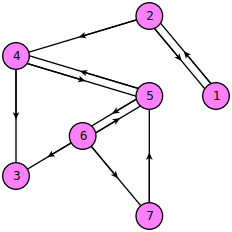
\includegraphics{seven_page_1}} 
\caption{A seven page internet}
\label{F:seven_page}
\end{center}
\end{figure}


To rank pages, we need to know how likely it is that a surfer will land on a given page. In our seven page example, a person can land on page 3 from page 4 with a probability of $\frac{1}{2}$ or from page 6 with a probability of $\frac{1}{3}$. If there is a link from a page we assume that the surfer leaves the page, and if there are no links from a page then the surfer stays on that page. We also assume that the surfer does not use the ``Back'' key. This information for our seven page internet example can be summarized in a \emph{transition matrix} $T$ whose $i,j$th entry is the probability that a surfer lands on page $i$ from page $j$.
\[T= \left[ \renewcommand{\arraystretch}{1.2} \begin{array}{ccccccc} 0&\frac{1}{2}&0&0&0&0&0 \\ 1&0&0&0&0&0&0 \\ 0&0&1&\frac{1}{2}&0&\frac{1}{3}&0 \\ 0&\frac{1}{2}&0&0&\frac{1}{2}&0&0 \\ 0&0&0&\frac{1}{2}&0&\frac{1}{3}&1 \\ 0&0&0&0&\frac{1}{2}&0&0 \\ 0&0&0&0&0&\frac{1}{3}&0 \end{array} \right].\]

Let us assume in our seven page internet that a user starts on page 6. That is, the probability that the user is initially on page 6 is 1, and so the probability that the user is on some other page is 0. This information can be encapsulated in a \emph{state vector}
\[\vx_0 = \left[ 0 \ 0 \ 0 \ 0 \ 0 \ 1 \ 0  \right]^{\tr}.\]
Since there are links from page 6 to pages 3, 5, and 7, there is a $\frac{1}{3}$ probability that the surfer will next move to one of these pages. That means that at the next step, the state vector $\vx_1$ for this user will be
\[\vx_1 = \left[ 0 \ 0 \ \frac{1}{3} \ 0 \ \frac{1}{3} \ 0 \ \frac{1}{3} \right]^{\tr}.\]
Note that
\[\vx_1 = T\vx_0.\]
As the user continues to surf the internet, the probabilities that the surfer is on a given page after the second, third, and fourth steps are given in the state vectors
\[\vx_2 = T\vx_1 = T^2 \vx_0, \ \ \vx_3 = T\vx_2 = T^3 \vx_0, \ \ \vx_4 = T\vx_3 = T^4 \vx_0.\]
In general, the probabilities that the surfer is on a given page after the $n$th step is given by the state vector
\[\vx_n = T \vx_{n-1} = T^n \vx_0.\]

This example illustrates the general nature of what is called a \emph{Markov process} (see Definition \ref{def:Markov}).  The two properties of the transition matrix $T$ make $T$ a special kind of matrix.

\begin{definition}  A \textbf{stochastic} matrix\index{stochastic matrix} is a matrix in which entries are nonnegative and the sum of the entries in every column is one.
\end{definition}

In a Markov process, each generation depends only on the preceding generation and there may be a limiting value as we let the process continue indefinitely. We can test to see if that happens for this Markov process defined by $T$ by doing some experimentation.


\begin{pactivity} \label{act:limit} Use appropriate technology to do the following. Choose several different initial state vectors $\vx_0$ and calculate the vectors in the sequence $\{T^n\vx_0\}$ for large values of $n$. (Note that, as state vectors, the entries of $\vx_0$ cannot be negative and the sum of the entries of $\vx_0$ must be $1$.) Explain the behavior of the sequence $\{\vx_n\}$ as $n$ gets large. Do you notice anything strange? What aspects of our seven page internet do you think explain this behavior? Clearly communicate all of the experimentation that you do. You may use the GeoGebra applet at \url{https://www.geogebra.org/m/b3dybnux}.  


\end{pactivity}



If there is a limit of the sequence $\{T^n\vx_0\}$ (in other words, if there is a vector $\vv$ such that $\vv = \ds \lim_{n \to \infty} T^n \vx_0$), we call this limit a \emph{steady-state} or \emph{equilibrium} vector. Such a steady-state vector has another important property. Since $T$ is independent of $n$ we have 
\begin{equation} \label{eq:Google_evector}
T \vv = T\left(\lim_{n \to \infty} T^n \vx_0 \right) = \lim_{n \to \infty} T^{n+1} \vx_0 = \vv.
\end{equation}


Equation (\ref{eq:Google_evector}) shows that a steady state vector $\vv$ is an eigenvector for $T$ with eigenvalue 1. We can interpret the steady-state vector for $T$ in an important way. Let $t_j$ be the fraction of time we spend on page $j$ and let $l_j$ be the number of links on page $j$. Then the fraction of the time that we end up on page $i$ coming from page $j$ is $\frac{t_j}{l_j}$. If we sum over all the pages linked to page $i$ we have that
\[t_i = \sum \frac{t_j}{l_j}.\]
Notice that this is essentially the same process we used to obtain $\vx_n$ from $\vx_{n-1}$, and so we can interpret the steady-state vector $\vv$ as telling us what fraction of a random web surfer's time was spent at each web page. If we assume that the time spent at a web page is a measure of its importance, then the steady-state vector tells us the relative importance of each web page. So this steady-state vector provides the page rankings for us. In other words,
\begin{quote}
The importance of a webpage may be measured by the relative size of the corresponding entry in the steady-state vector for an appropriately chosen Markov chain.
\end{quote}


\begin{pactivity} Show that the limiting vector you found in Project Activity \ref{act:limit} is an eigenvector of $T$ with eigenvalue 1.


\end{pactivity}


Project Activity \ref{act:limit} illustrates one problem with our seven page internet. The steady-state vector shows that page 3 is the only important page, but that hardly seems reasonable in the example since there are other pages that must have some importance. The problem is that page 3 is a ``dangling'' page and does not lead anywhere. Once a surfer reaches that page, they are  stuck there, overemphasizing its importance. So this dangling page acts like a sink, ultimately drawing all surfers to it. To adjust for dangling pages, we make the assumption that if a surfer reaches a dangling page (one with no links emanating from it), the surfer will jump to any page on the web with equal probability. So in our seven page example, once a surfer reaches page 3 the surfer will jump to any page on the web with probability $\frac{1}{7}$.

\begin{pactivity} \label{LQ:G2} ~
    \ba
    \item Determine the transition matrix for our seven page internet with this adjustment.

    \item Approximate the steady-state vector for this adjusted matrix so that the entries are accurate to four decimal places. Use any appropriate technology to row reduce matrices.
   

    \item According to this adjusted model, which web page is now the most important? Why? Does this seem reasonable? Why?


    \ea
\end{pactivity}

There is one more issue to address before we can consider ourselves ready to rank web pages. Consider the example of the five page internet shown in Figure \ref{F:five_page}.


\begin{figure}[h]
\begin{center}
\resizebox{!}{2.0in}{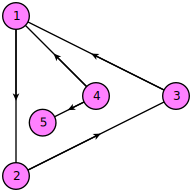
\includegraphics{five_page_1}} 
\caption{A five page internet}
\label{F:five_page}
\end{center}
\end{figure}


\begin{pactivity} \label{Q:no_limit} ~
    \ba
    \item Explain why
    \[\renewcommand{\arraystretch}{1.2} \left[ \begin{array}{ccccc} 0&0&1&\frac{1}{2}&\frac{1}{5} \\ 1&0&0&0&\frac{1}{5} \\ 0&1&0&0&\frac{1}{5} \\ 0&0&0&0&\frac{1}{5} \\ 0&0&0&\frac{1}{2}&\frac{1}{5} \end{array} \right].\]
is the transition matrix for this five page internet. (Keep in mind the adjustment we made for dangling pages.)

    \item Start with different initial state vectors $\vx_0$ and determine if there is a limit to the Markov chain. Explain. You may use the GeoGebra applet at \url{https://www.geogebra.org/m/b3dybnux}.  


    \ea
\end{pactivity}



Project Activity \ref{Q:no_limit} shows that it is possible to construct an internet so that the corresponding Markov chain does not have a limit, even after adjusting for dangling pages. This is a significant problem if we want to provide a relative ranking of all web pages regardless of where a surfer starts. To fix this problem we need to make one final adjustment to arrive at a type of transition matrix that always provides a limit for our Markov chain.

\begin{definition} A stochastic matrix is \textbf{regular}\index{stochastic matrix!regular} if its transition matrix $T$ has the property that for some power $k$, all the entries of $T^k$ are positive.
\end{definition}

Note that the transition matrix from Project Activity \ref{Q:no_limit} is not regular. Regular matrices have some especially nice properties, as the following theorem describes. We will not prove this theorem, but use it in the remainder of this project. The theorem shows that if we have a regular transition matrix, then there will a limit of the state vectors $\vx_n$, and that this limit has a very interesting property.

\begin{theorem} \label{thm:Google_1} Assume $n \geq 2$ and that $T$ is a regular $n \times n$ stochastic matrix.
\begin{enumerate}
\item $\ds \lim_{k \to \infty} T^k$ exists and is a stochastic matrix.
\item For any vector $\vx$,
\[\lim_{k \to \infty} T^k \vx = \vc\]
for the same vector $\vc$. 
\item The columns of $\ds \lim_{k \to \infty} T^k$ are the same vector $\vc$.
\item The vector $\vc$ is the unique eigenvector of $T$ whose entries sum to 1.
\item If $\lambda$ is an eigenvalue of $T$ not equal to 1, then $|\lambda| < 1$.
\end{enumerate}
\end{theorem}

 
Having a regular transition matrix $T$ ensures that there is always the same limit $\vv$ to the sequence $T^k \vx_0$ for any starting vector $\vx_0$. As mentioned before, the entries in $\vv = \ds \lim_{n \to \infty} T^n \vx_0$ can be interpreted as telling us what fraction of the random surfer's time was spent at each webpage. If we interpret the amount of time a surfer spends at a page as a measure of the page's importance, then this steady-state vector $\vv$ provides a ranking of the relative importance of each page in the web. This is the essence of Google's PageRank.

To make our final adjustment in the transition matrix to be sure that we obtain a regular matrix, we need to deal with the problems of ``loops'' in our internet. Loops, as illustrated in Project Activity \ref{Q:no_limit}, can act as sinks just like the dangling pages we saw earlier and condemn a user that enters such a loop to spend his/her time only on those pages in the loop. Quite boring! To account for this problem, we make a second adjustment.

Let $p$ be a number between 0 and 1 (Google supposedly uses $p=0.85$). Suppose a surfer is on page $i$. We assume with probability $p$ that the surfer will chose any link on page $i$ with equal probability. We make the additional assumption with probability $1-p$ that the surfer will select with equal probability any page on the web.

If $T$ is a transition matrix, incorporating the method we used to deal with dangling pages, then the adjusted transition matrix $G$ (the Google matrix) is
\[G = pT + (1-p)Q,\]
where $Q$ is the matrix all of whose entries are $\frac{1}{n}$, where $n$ is the number of pages in the internet ($n=7$ in our seven page example). Since all of the entries of $G$ are positive, $G$ is a regular stochastic matrix.



\begin{pactivity} Return to the seven page internet in Figure \ref{F:seven_page}.
    \ba
    \item Find the Google matrix $G$ for this internet.

    \item Approximate, to four decimal places, the steady-state vector for this internet. 

    \item What is the relative rank of each page in this internet, and approximately what percentage of time does a random user spend on each page.
    
    \ea
\end{pactivity}


We conclude with two observations. Consider the role of the parameter $p$ in our final adjustment. Notice that if $p=1$, then $G = T$ and we have the original hyperlink structure of the web. However, if $p=0$, then $G = \frac{1}{n} I_n$, where $I_n$ is the $n \times n$ identity matrix with $n$ as the number of pages in the web. In this case, every page is linked to every other page and a random surfer spends equal time on any page. Here we have lost all of the character of the linked structure of the web. Choosing $p$ close to 1 retains much of the original hyperlink structure of the web.

Finally, the matrices that model the web are HUGE, and so the methods we used in this project to approximate the steady-state vectors are not practical. There are many methods for approximating eigenvectors that are often used in these situations, some of which we discuss in a later section.






 %9
\achapter{10}{The Inverse of a Matrix} \label{sec:matrix_inverse}

\vspace*{-17 pt}
\framebox{
\parbox{\dimexpr\linewidth-3\fboxsep-3\fboxrule}
{\begin{fqs}
\item What does it mean for a matrix $A$ to be invertible? 
\item How can we tell when an $n \times n$ matrix $A$ is invertible?
\item If an $n \times n$ matrix $A$ is invertible, how do we find the inverse of $A$?
\item If $A$ and $B$ are invertible $n \times n$ matrices, why is $AB$ invertible and what is $(AB)^{-1}$?
\item How can we use the inverse of a matrix in solving matrix equations?
\end{fqs}}}% \hspace*{3 pt}}

\vspace*{13 pt}


\csection{Application: Modeling an Arms Race}

Lewis Fry Richardson was a Quaker by conviction who was deeply troubled by the major wars that had been fought in his lifetime. Richardson's training as a physicist led him to believe that the causes of war were phenomena that could be quantified, studied, explained, and thus controlled. He collected considerable data on wars and constructed a model to represent an arms race. The equations in his model caused him concern about the future as indicated by the following statement:  
\begin{quote} But it worried him that the equations also showed that the unilateral disarmament of Germany after 1918, enforced by the Allied Powers, combined with the persistent level of armaments of the victor countries would lead to the level of Germany�s armaments growing again. In other words, the post-1918 situation was not stable. From the model he concluded that great statesmanship would be needed to prevent an unstable situation from developing, which could only be prevented by a change of policies.\footnote{\emph{Nature} \textbf{135}, 830-831 (18 May 1935) ``Mathematical Psychology of War" (3420).}
\end{quote}
Analyzing Richardson's arms race model utilizes matrix operations, including matrix inverses. We explore the basic ideas in Richardson's model later in this section. 


\csection{Introduction}

To this point we have solved systems of linear equations with matrix forms $A \vx = \vb$ by row reducing the augmented matrices $[A \ | \ \vb]$. These linear matrix-vector equations should remind us of linear algebraic equations of the form $ax = b$, where $a$ and $b$ are real numbers. Recall that we solved an equation of the form $ax=b$ by dividing both sides by $a$ (provided $a \neq 0$), giving the solution $x = \frac{b}{a}$, or equivalently $x = a^{-1}b$. The important property that the number $a^{-1}$ has that allows us to solve a linear equation in this way is that $a^{-1}a = 1$, so that $a^{-1}$ is the multiplicative inverse of $a$. We can solve certain types of matrix equations $A \vx = \vb$ in the same way, provided we can find a matrix $A^{-1}$ with similar properties. We investigate this situation in this section.

\begin{pa} \label{pa:2_c} ~
\be
\item Before we define the inverse matrix, recall that the identity matrix $I_n$ (with 1's along the diagonal and 0's everywhere else) is a multiplicative identity in the set of $n \times n$ matrices (just like the real number 1 is the multiplicative identity in the set of real number). In particular, $I_nA = AI_n = A$ for any $n \times n$ matrix $A$. 

Now we can generalize the inverse operation to matrices. For an $n\times n$ matrix $A$, we define $A^{-1}$ to be the matrix which when multiplied by $A$ gives us the identity matrix. In other words, $AA^{-1}=A^{-1}A=I_n$. We can find the inverse of a matrix in a calculator by using the $x^{-1}$ button.

For each of the following matrices, determine if the inverse exists using your calculator or other appropriate technology. If the inverse does exist, write down the inverse and check that it satisfies the defining property of the inverse matrix, that is $AA^{-1}=A^{-1}A=I_n$. If the inverse doesn't exist, write down any error you received from the technology. Can you guess why the inverse does not exist for these matrices? \\

\ba
\begin{minipage}{2.0in}
\item $A = \left[ \begin{array}{cc} 1&3 \\ 0&4 \end{array} \right]$
\end{minipage}
\begin{minipage}{2.0in}
\item $A = \left[ \begin{array}{cc} 2&3 \\ 4&6 \end{array} \right]$
\end{minipage}

\begin{minipage}{2.0in}
\item $A = \left[ \begin{array}{rrc} 1&2&3 \\ -1&-1&2\\1&2&2 \end{array} \right]$
\end{minipage}
\begin{minipage}{2.0in}
\item $A = \left[ \begin{array}{rrc} 1&2&3 \\ 2&4&6\\1&2&2 \end{array} \right]$
\end{minipage}

\begin{minipage}{2.0in}
\item $A = \left[ \begin{array}{rrc} 1&0&0 \\ 0&2&0\\0&0&3 \end{array} \right]$
\end{minipage}
\begin{minipage}{2.0in}
\item $A = \left[ \begin{array}{rrc} 1&2&3 \\ -1&-1&2\\0&1&5 \end{array} \right]$
\end{minipage}

\ea

\item Now we turn to the question of how to find the inverse of a matrix in general. With this approach, we will be able to determine which matrices have inverses as well. 

We will consider the $2 \times 2$ case to make the calculations easier. Suppose $A$ is a $2 \times 2$ matrix. Our goal is to find a matrix $B$ so that $AB = I_2$ and $BA = I_2$. If such a matrix exists, we will call $B$ the inverse, $A^{-1}$, of $A$. 
	\ba
	\item What does the equation $AB = I_2$ tell us about the size of the matrix $B$?
		

	\item Now let $A = \left[ \begin{array}{cc} 1&2 \\ 1&3 \end{array} \right]$. We want to find a  matrix $B$ so that $AB = I_2$. Suppose $B$ has columns $\vb_1$ and $\vb_2$, i.e. $B = [\vb_1 \ \vb_2]$. Our definition of matrix multiplication shows that 
	\[AB = [A\vb_1 \ A\vb_2].\]
		\begin{enumerate}[i.]
		\item If $AB = I_2$, what must $A\vb_1$ and $A \vb_2$ equal? 
		
		\item Use the result from part (a) to set up two matrix equations to solve to find $\vb_1$ and $\vb_2$. Then find $\vb_1$ and $\vb_2$. As a result, find the matrix $B$.

		\item When we solve the two systems we have found a matrix $B$ so that $AB = I_2$. Is this enough to say that $B$ is the inverse of $A$? If not, what else do we need to know to verify that $B$ is in fact $A^{-1}$? Verify that $B$ is $A^{-1}$. 
	
		\end{enumerate}
	\ea

\item A matrix inverse is extremely useful in solving matrix equations and can help us in solving systems of equations. Suppose that $A$ is an invertible matrix, i.e., there exists $A^{-1}$ such that $AA^{-1}=A^{-1}A=I_n$.

\ba 

\item Consider the system $A\vx=\vb$. Use the inverse of $A$ to show that this system has a solution for every $\vb$ and find an expression for this solution in terms of $\vb$ and $A^{-1}$. (Note that since matrix multiplication is not commutative, we have to pay attention to the order in which we multiply matrices. For example, $A^{-1}AB=B$ while we cannot simplify $ABA^{-1}$ to $B$ unless $A$ and $B$ commute.)

\item If $A$, $B$, and $C$ are matrices and $A+C = B+C$, then we can subtract the matrix $C$ from both sides to see that $A = B$. We saw in Section \ref{sec:matrix_operations} that there is no corresponding general cancellation property for matrix multiplication when we found that $AB=AC$ could hold while $B\neq C$. However, we can cancel $A$ from this equation in certain circumstances. Suppose that $AB=AC$ and that $A$ is an invertible matrix. Show that we can cancel $A$ in this case and conclude that $B=C$. (Note: When simplifying the product of matrices, again keep in mind that matrix multiplication is not commutative.)

\ea

\ee

\end{pa}


\csection{Invertible Matrices} 

We now have an algebra of matrices in that we can add, subtract, and multiply matrices of the correct sizes. But what about division? In our early mathematics education we learned about \emph{multiplicative inverses} (or reciprocals) of real numbers. The multiplicative inverse of a number $a$ is the real number which when multiplied by $a$ produces 1, the multiplicative identity of real numbers. This inverse is denoted $a^{-1}$. For example, the multiplicative inverse of $2$ is $2^{-1}=\frac{1}{2}$ because 
\[2\cdot \frac{1}{2} = 1 = \frac{1}{2}\cdot 2.\]
Of course, we didn't have to write both products because multiplication of real numbers is a commutative operation.  There are a couple of important things to note about multiplicative inverses -- we can use the inverses of the number $a$ to solve the simple linear equation $ax+b = c$ for $x$ ($x = a^{-1}(c-b)$), and not every real number has an inverse. The latter means that the inverse is not defined on the entire set of real numbers. We can extend the idea of inverses to matrices, although we will see that there are many more matrices than just the zero matrix that do not have inverses.

To define matrix inverses\footnote{We usually refer to a multiplicative inverse as just an inverse. Since every matrix has an additive inverse, there is no need to consider the existence of additive inverses.} we make an analogy with the property of inverses in the real numbers: $x\cdot x^{-1}=1=x^{-1}\cdot x$. 



\begin{definition} Let $A$ be an $n \times n$ matrix.
\begin{enumerate}
\item $A$ is \textbf{invertible}\index{matrix!invertible} if there is an $n \times n$ matrix $B$ so that $AB = BA = I_n$. 
\item If $A$ is invertible, an \textbf{inverse}\index{matrix!inverse} of $A$ is a matrix $B$ such that $AB = BA = I_n$. 
\end{enumerate} 
\end{definition}



If an $n \times n$ matrix $A$ is invertible, its inverse will be unique (see Exercise \ref{ex:2_c_unique_inverse}), and we denote the inverse of $A$ as $A^{-1}$. We also call an invertible matrix a \emph{non-singular}\index{matrix!non-singular} matrix (with \emph{singular}\index{matrix!singular} meaning non-invertible). 



\begin{activity} \label{act:2_c_1} ~
	\ba
	\item Let $A = \left[ \begin{array}{cc} 1 & 0 \\ 0 & 0 \end{array} \right]$. Calculate $AB$ where $B = \left[ \begin{array}{cc} a&b \\ c&d \end{array} \right]$. Using your result, explain why it is not possible to have $AB=I_2$, showing that $A$ is non-invertible. 



\item Calculate $AB$ where $A = \left[ \begin{array}{cc} 1 & 2 \\ 2 & 4 \end{array} \right]$ and $B = \left[ \begin{array}{cc} a&b \\ c&d \end{array} \right]$. Using your result, explain why the inverse of $A$ doesn't exist.

	
	
	\ea
	
\end{activity}

We saw in Activity \ref{act:2_c_1} why the inverse does not exist for two specific matrices. We will find in the next section an easy criterion for determining when a matrix has an inverse. In short, when the RREF of the matrix has a pivot in every column and row, then the matrix will be invertible. We know that this condition relates to quite a few other linear algebra concepts we have seen so far, such as linear independence of columns and the columns spanning $\R^n$. We will put these criteria together in one big theorem in the next section.



\begin{activity} \label{act:2_c_2} Suppose that $A$ is an invertible $n \times n$ matrix. Hence we have an inverse matrix $A^{-1}$ for which $AA^{-1}=A^{-1}A=I_n$. We will see how the inverse is useful in solving matrix equations involving $A$.

	\ba
	\item Explain why the matrix expressions 
\[\ A^{-1}(AB) , \ A^{-1}(A(BA)A^{-1}) \ \text{ and } \ BA^{-1}BAA^{-1}B^{-1}A\]
can all be simplified to $B$. (Hint: Use the associative property of matrix multiplication.)
	
	
	
	\item Suppose the system $A \vx = \vb$ has a solution. Explain why then $A^{-1}(A\vx)= A^{-1}\vb$. What does this equation simplify to?
	
	
	
	\item Since we found one single expression for the solution $\vx$ in equation $A\vx=\vb$, this implies that the equation has a unique solution. What does this imply about the matrix $A$? 
	
	
	
	\ea
	
\end{activity}



As we saw in Preview Activity \ref{act:2_c_1}, if the $n \times n$ matrix $A$ is invertible, then the equation $A \vx = \vb$ is consistent for all $\vb$ in $\R^n$ and has the unique solution $\vx = A^{-1} \vb$. This means that $A$ has a pivot in every row and column, which is equivalent to the criterion that $A$ reduces to $I_n$, as we noted above. 

Even though $\vx=A^{-1}\vb$ is an explicit expression for the solution of the system $A\vx=\vb$, using the inverse of a matrix is usually not a computationally efficient way to solve a matrix equation. Finding the RREF of a matrix computationally takes fewer steps to solve the matrix equation. 


\csection{Finding the Inverse of a Matrix}

The next questions for us to address are how to tell when a matrix is invertible and how to find the inverse of an invertible matrix. Consider a $2 \times 2$ matrix $A$. To find the inverse matrix $B = [\vb_1 \ \vb_2]$ of $A$, we have to solve the two matrix-vector equations $A \vb_1 = \begin{bmatrix}1 \\ 0 \end{bmatrix}$ and $A \vb_2= \begin{bmatrix}0 \\1 \end{bmatrix}$ to find the columns of $B$. Since $A$ is the coefficient matrix for both systems, we apply the same row operations on both systems to reduce $A$ to RREF. Thus, instead of solving the two matrix-vector equations separately, we could simply have found the RREF of 
\[\left[\, A \ \left| \begin{array}{cc} 1 & 0 \\ 0 & 1 \end{array}\right. \right]\]
and done all of the work in one pass. Note that the right hand side of the augmented matrix is now $I_2$. So we row reduce $[A \ | \ I_2]$, and if the systems are consistent, the reduced row echelon form of $[A \ | \ I_2]$ must be $[I_2 \ | \ A^{-1}]$.  You should be able to see that this same process works in any dimension. 



\noindent \textbf{How to find the inverse of an $n \times n$ matrix $A$:}
\begin{itemize}
\item Augment $A$ with the identity matrix $I_n$.
\item Apply row operations to reduce the augmented matrix $[A \ | \ I_n]$. If the system is consistent, then the reduced row echelon form of $[A \ | \ I_n]$ will have the form $[I_n \ | \ B]$ (by Activity \ref{act:2_c_1} (d)). If the reduced row echelon form of $A$ is not $I_n$, then this step fails and $A$ is not invertible.
\item If $A$ is row equivalent to $I_n$, then the matrix $B$ in the second step has the property that $AB = I_n$. We will show later that the matrix $B$ also satisfies $BA = I_n$ and so $B$ is the inverse of $A$.
\end{itemize}



\begin{activity}  \label{act:2_c_3} Find the inverse of each matrix \underline{using the method above}, if it exists. Compare the result with the inverse that you get from using appropriate technology to directly calculate the inverse. 
\ba
\item $\left[ \begin {array}{crr} 1&1&1\\ 1&1&-1\\ 1&-1&0 \end {array} \right]$



\item $\left[ \begin {array}{cccc} 1&1&1\\ 2&2&2\\ 0&0&1 \end {array} \right]$

\ea

\end{activity}



We can use this method of finding the inverse of a matrix to derive a concrete formula for the inverse of a $2 \times 2$ matrix: 
\begin{equation} \label{eq:2_c_1}
\left[ \begin{array}{cc} a&b \\ c&d \end{array} \right]^{-1} = \frac{1}{ad-bc} \left[ \begin{array}{rr} d&-b \\ -c&a \end{array} \right],
\end{equation}
provided that $ad-bc \neq 0$ (see Exercise \ref{ex:2_c_2by2_inverse}). Hence, any $2\times 2$ matrix $\left[ \begin{array}{cc} a&b \\ c&d \end{array} \right]$ has an inverse if and only if $ad-bc\neq 0$. We call this quantity \emph{determinant of $A$}, $\det(A)$. We will see that the determinant of a general $n\times n$ matrix will be essential in determining invertibility of the matrix.


\csection{Properties of the Matrix Inverse}

As we have done with every new operation, we ask what properties the inverse of a matrix has. 



\begin{activity} \label{act:2_c_5} Consider the following questions about matrix inverses. If two $n \times n$ matrices $A$ and $B$ are invertible, is the product $AB$ invertible? If so, what is the inverse of $AB$? We answer these questions in this activity.
\ba
\item Let 
\[A = \left[ \begin{array}{cc} 1&2\\1&3 \end{array} \right] \ \ \text{ and }  B = \left[ \begin{array}{rc} 2&3\\-1&2 \end{array} \right].\]
	\begin{enumerate}[i.]
	\item Use formula (\ref{eq:2_c_1}) to find the inverses of $A$ and $B$.



	\item Find the matrix product $AB$. Is $AB$ invertible? If so, use formula (\ref{eq:2_c_1}) to find the inverse of $AB$.



	\item Calculate the products $A^{-1}B^{-1}$ and $B^{-1}A^{-1}$. What do you notice?   



	\end{enumerate}

\item In part (a) we saw that the matrix product $B^{-1}A^{-1}$ was the inverse of the matrix product $AB$. Now we address the question of whether this is true in general.  Suppose now that $C$ and $D$ are invertible $n \times n$ matrices so that the matrix inverses $C^{-1}$ and $D^{-1}$ exist. 
	\begin{enumerate}[i.]
	\item Use matrix algebra to simplify the matrix product $(CD)\left(D^{-1}C^{-1}\right)$. (Hint: What do you know about $DD^{-1}$ and $CC^{-1}$?)



	\item Simplify the matrix product $\left(D^{-1}C^{-1}\right)(CD)$ in a manner similar to part i.  
	
	
	
	\item What conclusion can we draw from parts i and ii? Explain. What property of matrix multiplication requires us to reverse the order of the product when we create the inverse of $CD$?  
	
	
	
	\end{enumerate}

\ea

\end{activity} 



Activity \ref{act:2_c_5} gives us one important property of matrix inverses. The other properties given in the next theorem can be verified similarly.



\begin{theorem} \label{thm:inverse_properties} Let $A$ and $B$ be invertible $n \times n$ matrices. Then
\begin{enumerate}
\item $\left(A^{-1}\right)^{-1} = A$.
\item The product $AB$ is invertible and  $(AB)^{-1} = B^{-1}A^{-1}$.
\item The matrix $A^{\tr}$ is invertible and $\left(A^{\tr}\right)^{-1} = \left(A^{-1}\right)^{\tr}$.
\end{enumerate}
\end{theorem}

\csection{Examples}

\ExampleIntro

\begin{example} For each of the following matrices $A$,
\begin{itemize}
\item Use appropriate technology to find the reduced row echelon form of $[A \ | \ I_3]$. 

\item Based on the result of part (a), is $A$ invertible? If yes, what is $A^{-1}$? If no, explain why.

\item Let $\vx = \left[ \begin{array}{c} x_1\\x_2\\x_3 \end{array} \right]$ and $\vb = \left[ \begin{array}{c} 5\\4\\1 \end{array} \right]$. If $A$ is invertible, solve the matrix equation $A \vx = \vb$ using the inverse of $A$. If $A$ is not invertible, find all solutions, if any, to the equation $A \vx = \vb$ using whatever method you choose. 
\end{itemize}

\ba
\item $A = \left[ \begin{array}{crr} 1&2&3 \\ 1&-1&-1 \\ 1&0&1 \end{array} \right]$
\item $A = \left[ \begin{array}{crr} 1&2&5 \\ 1&-1&-1 \\ 1&0&1 \end{array} \right]$
\ea

\ExampleSolution
\ba
\item With $A = \left[ \begin{array}{crr} 1&2&3 \\ 1&-1&-1 \\ 1&0&1 \end{array} \right]$, we have the following.
\begin{itemize}
\item The reduced row echelon form of $[A \ | \ I_3]$ is 
\[ \left[ \renewcommand{\arraystretch}{1.4}  \begin{array}{ccc|rrr} 1&0&0&\frac{1}{2}&1&-\frac{1}{2} \\ 0&1&0&1&1&-2  \\ 0&0&1&-\frac{1}{2}&-1&\frac{3}{2} \end{array} \right].\]
\item Since $A$ is row equivalent to $I_3$, we conclude that $A$ is invertible. The reduced row echelon form of $[A \ | \ I_3]$ tells us that 
\[A^{-1} = \frac{1}{2} \left[ \begin{array}{rrr} 1&2&-1 \\ 2&2&-4 \\ -1&-2&3 \end{array} \right].\]
\item The solution to $A \vx = \vb$ is given by 
\[vx = A^{-1} \vb = \frac{1}{2} \left[ \begin{array}{rrr} 1&2&-1 \\ 2&2&-4 \\ -1&-2&3 \end{array} \right] \left[ \begin{array}{c} 5\\4\\1 \end{array} \right] = \left[ \begin{array}{r} 6\\7\\-5 \end{array} \right].\]
\end{itemize}

\item With $A = \left[ \begin{array}{crr} 1&2&5 \\ 1&-1&-1 \\ 1&0&1 \end{array} \right]$, we have the following.
\begin{itemize}
\item The reduced row echelon form of $[A \ | \ I_3]$ is 
\[ \left[ \begin{array}{ccc|crr} 1&0&1&0&0&1 \\ 0&1&2&0&-1&1  \\ 0&0&0&1&2&-3 \end{array} \right].\]
\item Since $A$ is not row equivalent to $I_3$, we conclude that $A$ is not invertible. 
\item The reduced row echelon form of $[A \ | \ \vb]$ is 
\[ \left[ \begin{array}{ccc|c} 1&0&1&0 \\ 0&1&2&0 \\ 0&0&0&1 \end{array} \right].\]
The fact that the augmented column is a pivot column means that the equation $A \vx = \vb$ has no solutions. 
\end{itemize}

\ea


\end{example}

\begin{example} ~
\ba
\item Let $A = \left[ \begin{array}{ccc} 0&1&0\\0&0&1\\0&0&0 \end{array} \right]$. 
	\begin{enumerate}[i.]
	\item Show that $A^2 \neq 0$ but $A^3 = 0$. 
	
	\item Show that $I - A$ is invertible and find its inverse. Compare the inverse of $I-A$ to $I+A+A^2$. 
	
	\end{enumerate}

\item Let $M$ be an arbitrary square matrix such that $M^3 = 0$. Show that $M$ is invertible and find an inverse for $M$.

\ea


\ExampleSolution
\ba
\item Let $A = \left[ \begin{array}{ccc} 0&1&0\\0&0&1\\0&0&0 \end{array} \right]$. 
	\begin{enumerate}[i.]
	\item Using technology to calculate $A^2$ and $A^3$ we find that $A^3=0$ while $A^2 =  \left[ \begin{array}{ccc} 0&0&1\\0&0&0\\0&0&0 \end{array} \right]$.
	
	\item For this matrix $A$ we have $I - A = \left[ \begin{array}{crr} 1&-1&0\\0&1&-1\\0&0&1 \end{array} \right]$. The reduced row echelon form of $I-A$ is 
	\[\left[ \begin{array}{ccc|ccc} 1&-0&0&1&1&1\\0&1&0&0&1&1\\0&0&1&0&0&1 \end{array} \right],\]
	so $I-A$ is invertible and $(I-A)^{-1} = \left[ \begin{array}{ccc} 1&1&1\\0&1&1\\0&0&1 \end{array} \right]$. 
	
A straightforward matrix calculation also shows that 
\[(I-A)^{-1} = I+A+A^2.\]
	
	\end{enumerate}

\item We can try to emulate the result of part (a) here. Expanding using matrix operations gives us
\begin{align*}
(I-M)(I+M+M^2) &= (I+M+M^2) - (M+M^2+M^3) \\
	&= (I+M+M^2) - (M+M^2+0) \\
	&= I
\end{align*}
and
\begin{align*}
(I+M+M^2)(I-M) &= (I+M+M^2) - (M+M^2+M^3) \\
	&= (I+M+M^2) - (M+M^2+0) \\
	&= I.
\end{align*}	 
So $I-M$ is invertible and $(I-M)^{-1} = I+M+M^2$. 

This argument can be generalized to show that if $M$ is a square matrix and $M^n = 0$ for some positive integer $n$, then $I-M$ is invertible and 
\[(I-M)^{-1} = I+M+M^2+ \cdots + M^{n-1}.\] 

\ea


\end{example}

\csection{Summary}
\begin{itemize}
\item If $A$ is an $n \times n$ matrix, then $A$ is invertible if there is a matrix $B$ so that $AB = BA = I_n$. The matrix $B$ is called the inverse of $A$ and is denoted $A^{-1}$.
\item An $n \times n$ matrix $A$ is invertible if and only if $A$ the reduced row echelon form of $A$ is the $n \times n$ identity matrix $I_n$. 
\item To find the inverse of an invertible $n \times n$ matrix $A$, augment $A$ with the identity and row reduce. If $[A \ | \ I_n] \sim [I_n \ | \ B]$, then $B = A^{-1}$.
\item If $A$ and $B$ are invertible $n \times n$ matrices, then $(AB)^{-1}=B^{-1}A^{-1}$. Since the inverse of $AB$ exists, the product of two invertible matrices is an invertible matrix. 
\item We can use the algebraic tools we have developed for matrix operations to solve equations much like we solve equations with real variables. We must be careful, though, to only multiply by inverses of invertible matrices, and remember that matrix multiplication is not commutative. 
\end{itemize}




\csection{Exercises}

\be


\item \label{ex:2_c_unique_inverse} Let $A$ be an invertible $n \times n$ matrix. In this exercise we will prove that the inverse of $A$ is unique. To do so, we assume that both $B$ and $C$ are inverses of $A$, that is $AB=BA = I_n$ and $AC=CA = I_n$. By considering the product $BAC$ simplified in two different ways, show that $B=C$, implying that the inverse of $A$ is unique. 

\item \label{ex:2_c_2by2_inverse} Let $A = \left[ \begin{array}{cc} a&b \\ c&d \end{array} \right]$ be an arbitrary $2 \times 2$ matrix. 
	\ba
	\item If $A$ is invertible, perform row operations to determine a row echelon form of $A$. (Hint: You may need to consider different cases, e.g., when $a=0$ and when $a \neq 0$.)

	\item Under certain conditions, we can row reduce $[A \ | \ I_2]$ to $[I_2 \ | \ B]$, where 
\[B=\frac{1}{ad-bc} \left[ \begin{array}{rr} d&-b \\ -c&a \end{array} \right].\]
Use the row echelon form of $A$ from part (a) to find conditions under which the $2 \times 2$ matrix $A$ is invertible. Then derive the formula for the inverse $B$ of $A$. 
	\ea

\item \ba 
\item For a few different $k$ values, find the inverse of $A = \left[ \begin{array}{cc} 1&k \\ 0&1 \end{array} \right]$. From these results, make a conjecture as to what $A^{-1}$ is in general.

\item Prove your conjecture using the definition of inverse matrix. 

\item Find the inverse of $A = \left[ \begin{array}{ccc} 1&k&\ell \\ 0&1&m\\0&0&1 \end{array} \right]$.
\ea

(Note: You can combine the first two parts above by applying the inverse finding algorithm directly on $A = \left[ \begin{array}{cc} 1&k \\ 0&1 \end{array} \right]$.)

\item Solve for the matrix $A$ in terms of the others in the following equation:
\[ P^{-1}(D+CA)P=B\]
If you need to use an inverse, assume it exists.

\item For which $c$ is the matrix $A=\left[ \begin{array}{ccr} 1&2&-1\\2&1&1\\1&5&c\end{array} \right]$ invertible?

\item For which $c$ is the matrix $A=\left[ \begin{array}{cc} c&2\\3&c\end{array} \right]$ invertible?

\item Let $A$ and $B$ be invertible $n \times n$ matrices. Verify the remaining properties of Theorem \ref{thm:inverse_properties}. That is, show that 	
	\ba
	\item  $\left(A^{-1}\right)^{-1} = A$.
	\item The matrix $A^{\tr}$ is invertible and $\left(A^{\tr}\right)^{-1} = \left(A^{-1}\right)^{\tr}$.
	\ea

\item Label each of the following statements as True or False. Provide justification for your response.
\ba
\item \textbf{True/False} If $A$ is an invertible matrix, then for any two matrices $B, C$, $AB=AC$ implies $B=C$.

\item \textbf{True/False} If $A$ is invertible, then so is $AB$ for any matrix $B$.

\item \textbf{True/False} If $A$ and $B$ are invertible $n\times n$ matrices, then so is $AB$.


\item \textbf{True/False} If $A$ is an invertible $n\times n$ matrix, then the equation $A\vx=\vb$ is consistent for any $\vb$ in $\R^n$.

\item \textbf{True/False} If $A$ is an invertible $n\times n$ matrix, then the equation $A\vx=\vb$ has a unique solution when it is consistent.

\item \textbf{True/False} If $A$ is invertible, then so is $A^2$.

\item \textbf{True/False} If $A$ is invertible, then it reduces to the identity matrix.

\item \textbf{True/False} If a matrix is invertible, then so is its transpose.

\item \textbf{True/False} If $A$ and $B$ are invertible $n\times n$ matrices, then $A+B$ is invertible.

\item \textbf{True/False} If $A^2=0$, then $I+A$ is invertible.

\ea
\ee


\csection{Project: The Richardson Arms Race Model}

How and why a nation arms itself for defense depends on many factors. Among these factors are the offensive military capabilities a nation deems its enemies have, the resources available for creating military forces and equipment, and many others. To begin to analyze such a situation, we will need some notation and background. In this section we will consider a two nation scenario, but the methods can be extended to any number of nations. In fact, after World War I, Richardson collected data and created a model for the countries Czechoslovakia, China, France, Germany, England, Italy, Japan, Poland, the USA, and the USSR.\footnote{The Union of Soviet Socialist Republics (USSR), headed by Russia, was a confederation of socialist republics in Eurasia. The USSR disbanded in 1991. Czechoslovakia was a sovereign state in central Europe that peacefully split into the Czech Republic and Slovakia in 1993.}

Let $N_1$ and $N_2$ represent $2$ different nations. Each nation has some military capability (we will call this the \emph{armament} of the nation) at time $n$ (think of $n$ as representing the year). Let $a_1(n)$ represent the armament of nation $N_1$ at time $n$, and $a_2(n)$ the armament of nation $N_2$ at time $n$. We could measure $a_i(n)$ in weaponry or dollars or whatever units make sense for armaments. The Richardson arms race model provides connections between the armaments of the two nations. 

\begin{pactivity} \label{act:arms_race_1}  We continue to analyze a two nation scenario. Let us suppose that our two nations are Iran (nation $N_1$) and Iraq (nation $N_2$). In 1980, Iraq invaded Iran resulting in a long and brutal 8 year war. Richardson was interested in analyzing data to see if such wars could be predicted by the changes in armaments of each nation. We construct the two nation model in this activity. 
	
During each time period every nation adds or subtracts from its armaments. In our model, we will consider three main effects on the changes in armaments: the defense effect, fatigue effect and the grievance effect. In this activity we will discuss each effect in turn and then create a model to represent a two nation arms race. 
	
\begin{itemize}
\item We first consider the defense effect. In a two nation scenario, each nation may react to the potential threat implied by an arms buildup of the other nation. For example, if nation $N_1$ feels threatened by nation $N_2$ (think of South and North Korea, or Ukraine and Russia, for example), then nation $N_2$'s level of armament might cause nation $N_1$ to increase its armament in response. We will let $\delta_{12}$ represent this effect of nation $N_2$'s armament on the armament of nation $N_1$. Nation $N_1$ will then increase (or decrease) its armament in time period $n$ by the amount $\delta_{12}a_2(n-1)$ based on the armament of nation $N_2$ in time period $n-1$. We will call $\delta_{12}$ a \emph{defense coefficient}.\footnote{Of course, there are many other factors that have not been taken into account in the analysis. A nation may have heavily armed allies (like the U.S.) which may provide enough perceived security that this analysis is not relevant. Also, a nation might be a neutral state, such as Switzerland, and this analysis might not apply to such nations.}


\item Next we discuss the fatigue effect. Keeping a strong defense is an expensive and taxing enterprise, often exacting a heavy toll on the resources of a nation. For example, consider the fatigue that the U.S. experienced fighting wars in Iraq and Afghanistan, losing much hardware and manpower in these conflicts. Let $\delta_{ii}$ represent this \emph{fatigue factor} on nation $i$. Think of $\delta_{ii}$ as a measure of how much the nation has to replace each year, so a positive fatigue factor means that the nation is adding to its armament. The fatigue factor produces an effect of $\delta_{ii}a_i(n-1)$ on the armament of nation $i$ at time $t=n$ that is the effect of the armament at time $t=n-1$. 


\item The last factor we consider is what we will call a grievance factor. This can be thought of as the set of ambitions and/or grievances against other nations (such as the acquisition or reacquisition of territory currently belonging to another country). As an example, Argentina and Great Britain both claim the Falkland Islands as territory. In 1982 Argentina invaded the disputed Falkland Islands which resulted in a two-month long undeclared Falkland Islands war, which returned control to the British. It seems reasonable that one nation might want to have sufficient armament in place to support its claim if force becomes necessary. Assuming that these grievances and ambitions have a constant impact on the armament of a nation from year to year, let $g_i$ be this ``grievance" constant for nation $i$.\footnote{It might be possible for $g_i$ to be negative if, for example, a nation feels that such disputes can and should only be settled by negotiation.} The effect a grievance factor $g_i$ would have on the armament of nation $i$ in year $n$ would be to add $g_i$ directly to $a_i(n-1)$, since the factor $g_i$ is constant from year to year (paying for arms and soldier's wages, for example) and does not depend on the amount of existing armament.

\end{itemize} 

\ba
\item  Taking the three effects discussed above into consideration, explain why  
\[a_1(n) = \delta_{11}a_1(n-1) + \delta_{12}a_2(n-1) + a_1(n-1) + g_1.\]
Then explain why 
\begin{equation} \label{eq:AR_1}
a_1(n) = \left(\delta_{11}+1\right)a_1(n-1) + \delta_{12}a_2(n-1) + g_1. 
\end{equation}

\item Write an equation similar to equation (\ref{eq:AR_1})  that describes $a_2(n)$ in terms of the three effects. \\


\item Let $\va_n = \left[ \begin{array}{ccc} a_1(n) \\ a_2(n)  \end{array} \right]$. Explain why 
\[\va_n = (D+I_2)\va_{n-1} + \vg,\]
where $D = \left[ \begin{array}{cc} \delta_{11}&\delta_{12} \\ \delta_{21}&\delta_{22} \end{array} \right]$ and $\vg = [g_1 \ g_2]^{\tr}$. 


\ea

\end{pactivity}

\begin{table}[h]
\begin{center}
\begin{tabular}{lcc}
Year			& Iran 		& Iraq \\ \hline 
$1966$		&$662$		&$391$ \\ \hline	
$1967$		&$903$		&$378$ \\ \hline	
$1968$		&$1090$		&$495$ \\ \hline	
$1969$		&$1320$		&$615$ \\ \hline	
$1970$		&$1470$		&$600$ \\ \hline	
$1971$		&$1970$		&$618$ \\ \hline	
$1972$		&$2500$		&$589$ \\ \hline	
$1973$		&$2970$		&$785$ \\	 \hline
$1974$		&$5970$		&$2990$ \\ \hline 
$1975$		&$7100$		&$1690$
\end{tabular}
\caption{Military Expenditures of Iran and Iraq 1966-1975.}
\label{T:Expenditures}
\end{center}
\end{table}

\begin{pactivity} \label{act:arms_race_2} In order to analyze a specific arms race between nations, we need some data to determine values of the $\delta_{ij}$ and the $g_i$. Table \ref{T:Expenditures} shows the military expenditures of Iran and Iraq in the years leading up to their war in 1975. (The data is in millions of US dollars, adjusted for inflation and is taken from ``World Military Expenditures and Arms Transfers 1966-1975" by the U.S. Arms Control and Disarmament Agency.) We can perform regression (we will see how in a later section) on this data to obtain the following linear approximations:
\begin{align}
a_1(n) &= 2.0780a_1(n-1) - 1.7081a_2(n-1) - 126.9954 \label{eq:arms_race_regression_1} \\
a_2(n) &=  0.9419a_1(n-1) - 1.3283a_2(n-1) - 101.2980.  \label{eq:arms_race_regression_2}
\end{align}
(Of course, the data does not restrict itself to only factors between the two countries, so our model will not be as precise as we might like. However, it is a reasonable place to start.)  Use the regression equations (\ref{eq:arms_race_regression_1}) and (\ref{eq:arms_race_regression_2}) to explain why 
\[D = \left[ \begin{array}{cc} 1.0780&-1.7081 \\  0.94194&-2.3283 \end{array} \right] \ \text{ and } \ \ \vg = [ -126.9954 \ -101.2980]^{\tr}\]
for our Iran-Iraq arms race. 


\end{pactivity}


Activities \ref{act:arms_race_1} and \ref{act:arms_race_2} provide the basics to describe the general arms race model due to Richardson. If we have an $m$ nation arms race with $D = [\delta_{ij}]$ and $\vg = [g_i]$ , then 
\begin{equation} \label{eq:AR_model}
\va_n =  (D+I_m)\va_{n-1}+\vg.
\end{equation}


\begin{pactivity} The idea of an arms race, theoretically, is to reach a point at which all parties feel secure and no additional money needs to be spent on armament. If such a situation ever arises, then the armament of all nations is stable, or in equilibrium. If we have an equilibrium solution, then for large values of $n$ we will have $\va_n = \va_{n-1}$. So to find an equilibrium solution, if it exists, we need to find a vector $\va_E$ so that 
\begin{equation} \label{eq:AR_equilibrium}
\va_E = (D+I)\va_E + \vg
\end{equation}
where $I$ is the appropriate size identity matrix. If $\va_{E}$ exists, we call $\va_E$ an \emph{equilibrium state}.

We can apply matrix algebra to find the equilibrium state vector $\va_E$ under certain conditions. 
	\ba
   \item Assuming that $\va_E$ exists, use matrix algebra and Equation \ref{eq:AR_equilibrium} to show that 
    \begin{equation} \label{eq:AR_equilibrium_2}
    D\va_E + \vg = 0.
    \end{equation}


\item Under what conditions can we be assured that there will always be a unique equilibrium state $\va_{E}$? Explain. Under these conditions, how can we find this unique equilibrium state? Write this equilibrium state vector $\va_{E}$ as a matrix-vector product.

\item Does the arms race model for Iran and Iraq have an equilibrium solution? If so, find it. If not, explain why not. Use technology as appropriate. 

\item Assuming an equilibrium exists and that both nations behave in a way that supports the equilibrium, explain what the appropriate entry of the equilibrium state vector $\va_E$ suggests about what Iran and Iraq's  policies should be. What does this model say about why there might have been war between these two nations? 


\ea

\end{pactivity}



 %10
\achapter{11}{The Invertible Matrix Theorem} \label{chap:IMT}

\vspace*{-17 pt}
\framebox{
\parbox{\dimexpr\linewidth-3\fboxsep-3\fboxrule}
{\begin{fqs}
\item What does it mean for two statements to be equivalent? 
\item How can we efficiently prove that a string of statements are all equivalent?  
\item What is the Invertible Matrix Theorem and why is it important?  
\item What are the equivalent conditions to a matrix being invertible? 
\end{fqs}}}% \hspace*{3 pt}}

\vspace*{13 pt}


\csection{Introduction}
\label{sec:imt_intro}

This section is different than others in this book in that it contains only one long proof of the equivalence of statements that we have already discussed. As such, this is a theoretical section and there is no application connected to it. 

The Invertible Matrix Theorem is a theorem that provides many different statements that are equivalent to having a matrix be invertible. To understand the Invertible Matrix Theorem, we need to know what it means for two statements to be \emph{equivalent}\index{equivalent statements}. By equivalent, we mean that if one of the statements is true, then so is the other. We examine this idea in this preview activity.

\begin{pa} \label{pa:2_d} Let $A$ be an $n \times n$ matrix. In this activity we endeavor to understand why the two statements
\begin{description}
\item[I.] The matrix $A$ is invertible.
\item[II.] The matrix $A^{\tr}$ is invertible. 
\end{description}
are equivalent. To demonstrate that statements I and II are equivalent, we need to argue that if statement I is true, then so is statement II, and if statement II is true then so is statement I. 
\be
\item Let's first show that if statement I is true, then so is statement II. So we assume statement I. That is, we assume that $A$ is an invertible matrix. So we know that there is an $n \times n$ matrix $B$ such that $AB = BA = I_n$, where $I_n$ is the $n \times n$ identity matrix. To demonstrate that statement II must also be true, we need to verify that $A^{\tr}$ is an invertible matrix. 
	\ba
	\item What is $I_n^{\tr}$? 


	\item Take the transpose of both sides of the equation $AB = I_n$ and use the properties of the transpose to write $(AB)^{\tr}$ in terms of $A^{\tr}$ and $B^{\tr}$. 
	

	\item Take the transpose of both sides of the equation $BA = I_n$ and use the properties of the transpose to write $(BA)^{\tr}$ in terms of $A^{\tr}$ and $B^{\tr}$. 
	
	
	\item Explain how the previous two parts show that $B^{\tr}$ is the inverse of $A^{\tr}$, so that $A^{\tr}$ is invertible. So we have shown that if statement I is true, so is statement II.\footnote{Note that statement I does not have to be true. We are only assuming that IF statement I is true, then statement II must also be true.}


	\ea
	
\item Now we prove that if statement II is true, then so is statement I. So we assume statement II. That is, we assume that the matrix $A^{\tr}$ is invertible. We could do this in the same manner as part (a), or we could be a bit clever. Let's try to be clever.

	\ba
	\item What matrix is $\left(A^{\tr}\right)^{\tr}$? 

	
	\item Why can we use the result of part (a) with $A^{\tr}$ in place of $A$ to conclude that $A$ is invertible? As a consequence, we have demonstrated that $A$ is invertible if $A^{\tr}$ is invertible. This concludes our argument that statements I and II are equivalent. 
	
	\ea

\ee

\end{pa}



\csection{The Invertible Matrix Theorem}
\label{sec:imt}

We have been introduced to many statements about existence and uniqueness of solutions to systems of linear equations, linear independence of columns of coefficient matrices, onto linear transformations, and many other items. In this section we will analyze these statements in light of how they are related to invertible matrices, with the main goal to understand the Invertible Matrix Theorem. 

Recall that an $n \times n$ matrix $A$ is invertible if there is an $n \times n$ matrix $B$ such that $AB = BA = I_n$, where $I_n$ is the $n \times n$ identity matrix. The Invertible Matrix Theorem is an important theorem in that it provides us with a wealth of statements that are all equivalent to the statement that an $n \times n$ matrix $A$ is invertible, and connects many of the topics we have been discussing so far this semester into one big picture. 



\begin{theorem}[The Invertible Matrix Theorem]\index{Invertible Matrix Theorem} Let $A$ be an $n \times n$ matrix. The following statements are equivalent:
\begin{enumerate}
\item $A$ is an invertible matrix.
\item \label{item:trivial_soln} The equation $A \vx = \vzero$ has only the trivial solution.
\item $A$ has $n$ pivot columns. 
\item The columns of $A$ span $\R^n$.
\item $A$ is row equivalent to the identity matrix $I_n$.
\item The columns of $A$ are linearly independent.
\item The columns of $A$ form a basis for $\R^n$.
\item The matrix transformation $T$ from $\R^n$ to $\R^n$ defined by $T(\vx) = A\vx$ is one-to-one.
\item The matrix equation $A \vx = \vb$ has exactly one solution for each vector $\vb$ in $\R^n$.
\item The matrix transformation $T$ from $\R^n$ to $\R^n$ defined by $T(\vx) = A\vx$ is onto.
\item \label{item:AC_I} There is an $n \times n$ matrix $C$ so that $AC = I_n$.
\item \label{item:DA_I} There is an $n \times n$ matrix $D$ so that $DA = I_n$.
\item The scalar 0 is not an eigenvalue of $A$.
%\item $\det(A) \neq 0$.
\item $A^{\tr}$ is invertible.
\end{enumerate}
\end{theorem}




The Invertible Matrix Theorem is a theorem that provides many different statements that are equivalent to a matrix being invertible. As discussed in Preview Activity \ref{pa:2_d}, two statements are said to be \textbf{equivalent} if, whenever one of the statements is true, then the other is also true. So to demonstrate, say, statements I and II are equivalent, we need to argue that 
\begin{itemize}
\item if statement I is true, then so is statement II, and 
\item if statement II is true then so is statement I. 
\end{itemize}
The Invertible Matrix Theorem, however, provides a long list of statements that are equivalent. It would be inefficient to prove, one by one, that each pair of statements is equivalent. (There are $\binom{14}{2} = 91$ such pairs.) Fortunately, there is a shorter method that we can use. 



\begin{activity} \label{act:2_d_1} In this activity, we will consider certain parts of the Invertible Matrix Theorem and show that one implies another in a specific order. For all parts in this activity, we assume $A$ is an $n\times n$ matrix.

\ba
\item Consider the following implication: \\
$(2) \implies (6)$:\footnote{The symbol $\implies$ is the implication symbol, so $(1) \implies (12)$ is read to mean that statement $(1)$ of the theorem implies statement $(12)$.}  If the equation $A \vx = \vzero$ has only the trivial solution, then the columns of $A$ are linearly independent. This shows that part 2 of the IMT implies part 6 of the IMT. Justify this implication as if it is a T/F problem.

\item Justify the following implication:\\
$(6) \implies (9)$: If the columns of $A$ are linearly independent, then the matrix equation $A\vx =\vb$ has exactly one solution for each vector $\vb$ in $\R^n$.

\item Justify the following implication:\\
$(9) \implies (4)$: If the equation $A \vx = \vb$ has exactly one solution for every vector $\vb$ in $\R^n$, then the columns of $A$ span $\R^n$. \\

\item Justify the following implication:\\
$(4) \implies (2)$: If the columns of $A$ span $\R^n$, then the equation $A \vx = \vzero$ has only the trivial solution.\\

\item Using the above implications you proved, explain why we can conclude the following implication must also be true:\\
$(2) \implies (9)$: If the equation $A \vx = \vzero$ has only the trivial solution, then the matrix equation $A\vx =\vb$ has exactly one solution for each vector $\vb$ in $\R^n$.

\item Using the above implications you proved, explain why any one of the implications $(2)$, $(6)$, $(9)$, and $(4)$ implies any of the others.  

\ea

\end{activity}



Using a similar ordering of circular implications as in Activity \ref{act:2_d_1}, we can prove the Invertible Matrix Theorem by showing that each statement in the list implies the next statement, and that the last statement implies the first. 



\noindent \emph{Proof of the Invertible Matrix Theorem}

\begin{description}
\item[Statement (1) implies Statement (2).] This follows from work done in Activity \ref{act:2_d_1}. 
\item[Statement (2) implies Statement (3).] This was done in Activity \ref{act:2_d_1}. 
\item[Statement (3) implies Statement (4).] Suppose that every column of $A$ is a pivot column. The fact that $A$ is square means that every row of $A$ contains a pivot, and hence the columns of $A$ span $\R^n$.
\item[Statement (4) implies Statement (5).] Since the columns of $A$ span $\R^n$, it must be the case that every row of $A$ contains a pivot. This means that $A$ must be row equivalent to $I_n$. 
\item[Statement (5) implies Statement (6).] If $A$ is row equivalent to $I_n$, there must be a pivot in every column, which means that the columns of $A$ are linearly independent.
\item[Statement (6) implies Statement (7).] If the columns of $A$ are linearly independent, then there is a pivot in every column. Since $A$ is a square matrix, there is a pivot in every row as well. So the columns of $A$ span $\R^n$. Since they are also linearly independent, the columns form a minimal spanning set, which is a basis of $\R^n$.
\item[Statement (7) implies Statement (8).] If the columns form a basis of $\R^n$, then the columns are linearly independent. This means that each column is a pivot column, which also implies $A\vx=\vzero$ has a unique solution and that $T$ is one-to-one.
\item[Statement (8) implies Statement (9).] If $T$ is one-to-one, then $A$ has a pivot in every column. Since $A$ is square, every row of $A$ contains a pivot. Therefore, the system $A \vx = \vb$ is consistent for every $\vb \in \R^n$ and has a unique solution.
\item[Statement (9) implies Statement (10).] If $A\vx=\vb$ has a unique solution for every $\vb$, then the transformation $T$ is onto since $T(\vx)=\vb$ has a solution for every $\vb$.
\item[Statement (10) implies Statement (11).] Assume that $T$ defined by $T(\vx) = A\vx$ is onto. For each $i$, let $\ve_i$ be the $i$th column of the $n \times n$ identity matrix $I_n$. That is, $\ve_i$ is the vector in $\R^n$ with 1 in the $i$th component and 0 everywhere else. Since $T$ is onto, for each $i$ there is a vector $\vc_i$ such that $T(\vc_i) = A \vc_i = \ve_i$. Let $C = [\vc_1  \ \vc_2 \ \cdots \ \vc_n]$. Then
\[AC = A[\vc_1  \ \vc_2 \ \cdots \ \vc_n] = [A\vc_1 \ A\vc_2 \ \cdots \ A\vc_n] = [\ve_1 \ \ve_2 \ \cdots \ \ve_n] = I_n.\]
\item[Statement (11) implies Statement (12).] Assume $C$ is an $n \times n$ matrix so that $AC = I_n$. First we show that the matrix equation $C \vx = \vzero$ has only the trivial solution. Suppose $C \vx = \vzero$. Then
multiplying both sides on the left by $A$ gives us
\[A(C \vx) = A \vzero.\]
Simplifying this equation using $AC=I_n$, we find $\vx = \vzero.$

Since $C \vx = \vzero$ has only the trivial solution, every column of $C$ must be a pivot column. Since $C$ is an $n \times n$ matrix, it follows that every row of $C$ contains a pivot position. Thus, the matrix equation $C \vx = \vb$ is consistent and has a unique solution for every $\vb$ in $\R^n$. Let $\vv_i$ be the vector in $\R^n$ satisfying $C \vv_i = \ve_i$ for each $i$ between 1 and $n$ and let $M = [\vv_1 \ \vv_2 \ \cdots \ \vv_n]$. Then $CM = I_n$.

Now we show that $CA = I_n$. Since 
\[AC = I_n\]
we can multiply both sides on the left by $C$ to see that 
\[C(AC) = CI_n.\]
Now we multiply both sides on the right by $M$ and obtain
\[(C(AC))M = CM.\]
Using the associative property of matrix multiplication and the fact that $CM = I_n$ shows that 
\begin{align*}
(CA)(CM) &= CM \\
CA = I_n.
\end{align*}
Thus, if $A$ and $C$ are $n \times n$ matrices and $AC = I_n$, then $CA = I_n$. So we have proved our implication with $D = C$
\item[Statement (12) implies Statement (13).] Assume that there is an $n \times n$ matrix $D$ so that $DA = I_n$. Suppose $A \vx = \vzero$. Then multiplying both sides by $A$ on the left, we find that
\begin{align*}
D(A\vx) &= D\vzero \\
(DA) \vx &= \vzero \\
\vx &= \vzero.
\end{align*}
So the equation $A \vx = \vzero$ has only the trivial solution and $0$ is not an eigenvalue for $A$. 
\item[Statement (13) implies Statement (14).] If 0 is not an eigenvalue of $A$, then the equation $A \vx = \vzero$ has only the trivial solution. Since statement \ref{item:trivial_soln} implies statement \ref{item:AC_I}, there is an $n \times n$ matrix $C$ such that $AC = I_n$. The proof that statement \ref{item:AC_I} implies statement \ref{item:DA_I} shows that $CA = I_n$ as well. So $A$ is invertible. By taking the transpose of both sides of the equation $AA^{-1}=A^{-1}A=I_n$ (remembering $(AB)^{\tr}= B^{\tr}A^{\tr}$) we find
\[ (A^{-1})^{\tr} A^{\tr} = A^{\tr} (A^{-1})^{\tr} = I_n^{\tr}=I_n \,.\]
Therefore, $(A^{-1})^{\tr}$ is the inverse of $A^{\tr}$ by definition of the inverse.
\item[Statement (14) implies Statement (1).] Since statement (1) implies statement (14), we proved `If $A$ is invertible, then $A^{\tr}$ is invertible." Using this implication with $A^{\tr}$ replaced by $A$, we find that `If $A^{\tr}$ is invertible, then $(A^{\tr})^{\tr}$ is invertible." But $(A^{\tr})^{\tr}=A$, which proves that statement (14) implies statement (1).
\end{description}
This concludes our proof of the Invertible Matrix Theorem.


\csection{Examples}
\label{sec:imt_exam}

\ExampleIntro

\begin{example} Let $M = \left[ \begin{array}{cccc} 1&2&2&1 \\ 0&1&0&1 \\ 1&3&2&3 \\ 0&1&0&0 \end{array} \right]$. 
\ba
\item Without doing any calculations, is $M$ invertible? Explain your response.

\item Is the equation $M \vx = \vb$ consistent for every $\vb$ in $\R^4$? Explain.

\item Is the equation $M \vx = \vzero$ consistent? If so, how many solutions does this equation have? Explain. 

\item Is it possible to find a $4 \times 4$ matrix $P$ such that $PM = I_4$? Explain.

\ea


\ExampleSolution
\ba
\item The third column of $M$ is twice the first, so the columns of $M$ are not linearly independent. We conclude that $M$ is not invertible.

\item The equation $M \vx = \vb$ is not consistent for every $\vb$ in $\R^4$. If it was, then the columns of $M$ would span $\R^4$ and, since there are exactly four columns, the columns of $M$ would be a basis for $\R^4$. Thus, $M$ would have to be invertible, which it is not.

\item The homogeneous system is always consistent. Since the columns of $M$ are linearly dependent, the equation $M \vx = \vzero$ has infinitely many solutions.

\item It is not possible to find a $4 \times 4$ matrix $P$ such that $PM = I_4$. Otherwise $M$ would have to be invertible. 

\ea

\end{example}



\begin{example} Let $M$ be an $n \times n$ matrix whose eigenvalues are all nonzero.
\ba
\item Let $\vb \in \R^n$. Is the equation $M \vx = \vb$ consistent? If yes, explain why and find all solutions in terms of $M$ and $\vb$. If no, explain why.

\item Let $S$ be the matrix transformation defined by $S(\vx) = M\vx$. Suppose $S(\va) = S(\vb)$ for some vectors $\va$ and $\vb$ in $\R^n$. Must there be any relationship between $\va$ and $\vb$? If yes, explain the relationship. If no, explain why.

\item Let $\vm_1$, $\vm_2$, $\ldots$, $\vm_n$ be the columns of $M$. In how many ways can we write the zero vector as a linear combination of $\vm_1$, $\vm_2$, $\ldots$, $\vm_n$? Explain.

\ea
  


\ExampleSolution
\ba
\item Since $0$ is not an eigenvalue of $M$, we know that $M$ is invertible. Therefore, the equation $M \vx = \vb$ has the unique solution $\vx = M^{-1} \vb$.

\item The fact that $M$ is invertible implies that $S$ is one-to-one. So if $S(\va) = S(\vb)$, then it must be the case that $\va = \vb$. 

\item Because $M$ is invertible, the columns of $M$ are linearly independent. Therefore, there is only the trivial solution to the equation 
\[x_1\vm_1 + x_2\vm_2 +  \cdots + x_n\vm_n = \vzero.\] 

\ea

\end{example}

\csection{Summary}
\label{sec:imt_summ}
\begin{itemize}
\item Two statements are equivalent if, whenever one of the statements is true, then the other must also be true. 
\item To efficiently prove that a string of statements are all equivalent, we can prove that each statement in the list implies the next statement, and that the last statement implies the first.  
\item The Invertible Matrix Theorem gives us many conditions that are equivalent to an $n \times n$ matrix being invertible. This theorem is important because it connects many of the concepts we have been studying. 
\end{itemize}


\csection{Exercises}
\label{sec:imt_exer}

\be
\item Consider the matrix $A=\left[ \begin{array}{rcc} 1&2&a \\ -1&1&b \\ 1&1&c \end{array} \right]$. Use the Invertible Matrix Theorem to geometrically describe the vectors $\left[ \begin{array}{c} a \\ b\\ c\end{array} \right]$ which make $A$ invertible without doing any calculations.

\item Suppose $A$ is an invertible $n\times n$ matrix. Let $T$ be the matrix transformation defined by $T(\vx)=A\vx$ for $\vx$ in $\R^n$. Show that the matrix transformation $S$ defined by $S(\vx)=A^{-1}\vx$ is the inverse of the transformation $T$ (i.e., $S$ is the inverse function to $T$ when the transformations are considered as functions).

\item Label each of the following statements as True or False. Provide justification for your response.
\ba
\item \textbf{True/False} If $A^2$ is invertible, then $A$ is invertible.

\item \textbf{True/False} If $A$ and $B$ are square matrices with $AB$ invertible, then $A$ and $B$ are invertible.

\item \textbf{True/False} If the columns of an $n \times n$ matrix $A$ span $\R^n$, then the equation $A^{-1}\vx =\vzero$ has a unique solution.

\item \textbf{True/False} If the columns of $A$ and columns of $B$ form a basis of $\R^n$, then so do the columns of $AB$.

\item \textbf{True/False} If the columns of a matrix $A$ form a basis of $\R^n$, then so do the rows of $A$.

\item \textbf{True/False} If the matrix transformation $T$ defined by $T(\vx)=A\vx$ is one-to-one for an $n\times n$ matrix $A$, then the columns of $A^{-1}$ are linearly independent.

\item \textbf{True/False} If the columns of an $n\times n$ matrix $A$ span $\R^n$, then so do the rows of $A$.

\item \textbf{True/False} If there are two $n\times n$ matrices $A$ and $B$ such that $AB=I_n$, then the matrix transformation defined by $T(\vx)=A^T\vx$ is one-to-one.

\ea
\ee

 %11

%\end{comment}

%\begin{comment}

\part{The Vector Space $\R^n$}

\achapter{12}{The Structure of $\R^n$} \label{chap:R_n}

\vspace*{-17 pt}
\framebox{
\parbox{\dimexpr\linewidth-3\fboxsep-3\fboxrule}
{\begin{fqs}
\item What properties make $\R^n$ a vector space?
\item What is a subspace of $\R^n$?
\item What properties do we need to verify to show that a set of vectors is a subspace of $\R^n$? Why?
\item What important structure does the span of a set of vectors in $\R^n$ have?  
%\item What is an eigenspace of a matrix? 
\end{fqs}}}% \hspace*{3 pt}}

\vspace*{13 pt}

\csection{Application: Connecting GDP and Consumption in Romania}
\label{sec:appl_romania}

It is common practice in the sciences to run experiments and collect data. Once data is collected it is necessary to find some way to analyze the data and predict future behavior from the data. One method is to find a curve that best ``fits" the data, and one widely used method for curve fitting is called the \emph{least squares} method.

For example, economists are often interested in \emph{consumption}, which is the purchase of goods and services for use by households. In ``A Statistical Analysis of GDP and Final Consumption Using Simple Linear Regression, the Case of Romania 1990-2010",\footnote{B\u{a}l\u{a}cescu, Aniela \& Zaharia, Marian. (2012). A STATISTICAL ANALYSIS OF GDP AND FINAL CONSUMPTION USING SIMPLE LINEAR REGRESSION. THE CASE OF ROMANIA 1990?2010. Annals - Economy Series. 4. 26-31. Available from: \url{https://www.researchgate.net/publication/227382939_A_STATISTICAL_ANALYSIS_OF_GDP_AND_FINAL_CONSUMPTION_USING_SIMPLE_LINEAR_REGRESSION_THE_CASE_OF_ROMANIA_1990-2010}.} the authors collect data and then use simple linear regression to compare GDP (gross domestic product) to consumption in Romania. The data they used is seen in Table \ref{T:GDP_consumption}, with a corresponding scatterplot of the data (with consumption as independent variable and GDP as dependent variable). The units for GDP and consumption are milliions of leu (the currency of Romania is the leu -- on December 21, 2018, one leu was worth approximately \$0.25 U.S.)
The authors conclude their paper with the following statement: 
\begin{quote}
``However, we can appreciate that linear regression model describes the correlation between the value of gross domestic product and the value of final consumption and may be transcribed following form: 
\begin{center} PIB = -3127.51+ 1.22 CF. \end{center}

Analysis of correlation between GDP and final consumption (private consumption and public consumption) will result in an increase of 1.22 units of monetary value of gross domestic product. 
 
We can conclude that the Gross Domestic Product of our country is strongly influenced by the private and public consumption."
 \end{quote}

\begin{figure}[ht]
\begin{center}
\begin{minipage}{1.75in}
\begin{center}
\setlength{\tabcolsep}{2pt}
\hspace{-0.5in} \begin{tabular}{ccc} \hline
Year		&\hspace{0.2in} GDP \hspace{0.2in}		&Consumption \\ \hline
$1990$ 	&$85.8$ 		&$68.0$ \\ \hline
$1991$ 	&$220.4$ 		&$167.3$ \\ \hline
$1992$ 	&$602.9$ 		&$464.3$ \\ \hline
$1993$ 	&$2003.9$ 	&$1523.6$ \\ \hline
$1994$ 	&$4977.3$	&$3845.2$ \\ \hline
$1995$ 	&$7648.9$	&$6257.7$ \\ \hline
$1996$ 	&$11384.2$ 	&$9713.8$ \\ \hline
$1997$ 	&$25529.8$	&$ 21972.2$ \\ \hline
$1998$ 	&$37055.1$ 	&$33311.2$ \\ \hline
$1999$ 	&$55191.4$	&$49311.9$ \\ \hline
$2000$ 	&$80984.6$ 	&$69587.4$  \\ \hline
$2001$ 	&$117945.8$ 	&$100731.7$ \\ \hline
$2002$ 	&$152017.0$ 	&$127118.8$ \\ \hline
$2003$	&$197427.6$ 	&$168818.7$ \\ \hline
$2004$  	&$247368.0$ 	&$211054.6$ \\ \hline
$2005$ 	&$288954.6$  	&$251038.1$ \\ \hline
$2006$  	&$344650.6$  	&$294867.6$  \\ \hline
$2007$  	&$416006.8$  	&$344937.0$ \\ \hline
$2008$  	&$514700.0$  	&$420917.5$ \\ \hline
$2009$  	&$498007.5$  	&$402246.0$ \\ \hline 
$2010$  	&$513640.8$  	&$405422.4$ \\ \hline  
\end{tabular}
\captionof{table}{GDP and consumption in Romania.}
\label{T:GDP_consumption}
\end{center}
\end{minipage} \hspace{0.25in}
\begin{minipage}{2.0in}
\begin{center}
\resizebox{!}{2.0in}{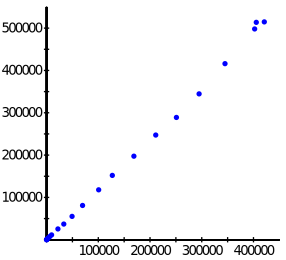
\includegraphics{GDP_consumption}}
\end{center}
\captionof{figure}{GDP and consumption data plot.}
\label{F:GDP_consumption}
\end{minipage}
\end{center}
\end{figure}


As we can see from the scatterplot, the relationship between the GDP and consumption is not exactly linear, but looks to be very close. To make correlations between GDP and consumption as the authors did, we need to understand how they determined their approximate linear relationship between the variables.  With a good approximation function we can then compare the variables, extrapolate from the data, and make predictions or interpolate and estimate between data points. For example, we could use our approximation function to predict, as the authors did, how changes in consumption affect GDP (or vice versa). Later in this section we will see how to find the least squares line to fit this data -- the best linear approximation to the data. This involves finding a vector in a certain subspace of $\R^2$ that is closest to a given vector. Linear least squares approximation is a special case of a more general process that we will encounter in later sections where we learn how to project sets onto subspaces. 


\csection{Introduction}
\label{sec:rn_intro}

The set $\R^n$ with vector addition and scalar multiplication has a nice algebraic structure. These operations satisfy a number of properties, such as associativity and commutativity of vector addition, the existence of an additive identity and additive inverse, distribution of scalar multiplication over vector addition, and others. These properties make it easier to work with the whole space since we can express the vectors as linear combinations of basis vectors in a unique way. This algebraic structure makes $\R^n$ a \emph{vector space}. 

There are many subsets of $\R^n$ that have this same structure. These subsets are called \emph{subspaces} of $\R^n$. These are the sets of vectors for which the addition of any two vectors is defined within the set, the scalar multiple of any vector by any scalar is defined within the set and the set contains the zero vector. One type of subset with this structure is the span of a set of vectors. 
 
Recall that the span of a set of vectors $\{\vv_1, \vv_2, \ldots, \vv_k\}$ in $\R^n$ is the set of all linear combinations of the vectors. For example, if $\vv_1=\left[ \begin{array}{c} 1\\1\\0\end{array} \right]$ and $\vv_2=\left[ \begin{array}{c} 1\\0\\1\end{array} \right]$, then a linear combination of these two vectors is of the form
\[ c_1 \vv_1 + c_2 \vv_2 = c_1 \left[ \begin{array}{c} 1\\1\\0\end{array} \right] + c_2 \left[ \begin{array}{c} 1\\0\\1\end{array} \right] = \left[ \begin{array}{c} c_1+c_2 \\c_1 \\c_2 \end{array} \right] \,. \]
One linear combination can be obtained by letting $c_1=2, c_2=-3$, which gives the vector $2\vv_1-3\vv_2=\left[ \begin{array}{c} -1\\-3\\2\end{array} \right]$. All such linear combinations form the span of the vectors $\vv_!$ and $\vv_2$. In this case, these vectors will form a plane through the origin in $\R^3$. 

Now we will investigate if the span of two vectors form a subspace, i.e. if it has the same structure as a vector space.


\begin{pa} \label{pa:3_a} Let $\vw_1$ and $\vw_2$ be two vectors in $\R^n$. Let $W = \Span \{\vw_1, \vw_2\}$. 
\be
\item For $W$ to be a subspace of $\R^n$, the sum of any two vectors in $W$ must also be in $W$.
    \ba
    \item Pick two specific examples of vectors $\vu, \vy$ in $W$ (keeping $\vw_1, \vw_2$ unknown/general vectors). For example, one specific $\vu$ would be $2\vw_1-3\vw_2$ as we used in the above example. Find the sum of $\vu, \vy$. Is the sum also in $W$? Explain. (Hint: What does it mean for a vector to be in $W$?)
		
		
		
		\item Now let $\vu$ and $\vy$ be arbitrary vectors in $W$. Explain why $\vu + \vy$ is in $W$.

    



	\ea
	
\item For $W$ to be a subspace of $\R^n$, any scalar multiple of any vector in $W$ must also be in $W$. 

	\ba 
	\item Pick a specific example $\vu$ in $W$. Explain why $2\vu, -3\vu, \pi\vu$ are all also in $W$.



	\item Now let $a$ be an arbitrary scalar and let $\vu$ be an arbitrary vector in $W$. Explain why the vector $a \vu$ is in $W$.

    
		
		
	\ea


\item For $W$ to be a subspace of $\R^n$, the zero vector must also be in $W$. Explain why the zero vector is in $W$. 

    
		
		


\item Does vector addition being commutative for vectors in $\R^n$ imply that vector addition is also commutative for vectors in $W$? Explain your reasoning.






\item Suppose we have an arbitrary $\vu$ in $W$. There is an additive inverse of $\vu$ in $\R^n$. In other words, there is a $\vu'$ such that $\vu+
\vu'=\vzero$. Should this $\vu'$ be also in $W$? If so, explain why. If not, give a counterexample.



\item Look at the other properties of vector addition and scalar multiplication of vectors in $\R^n$ listed in Theorem \ref{thm:vector_properties} in Section \ref{sec:vector_representation}. Which of these properties should also hold for vectors in $W$? 




    
\ee
    
\end{pa}


%The result of the first three problems above is that $W$ is a subspace of $\R^n$. Since the other properties of vector addition and scalar multiplication in the space $\R^n$ (such as commutativity and associativity of vector addition, existence of an additive inverse, distribution of scalar multiplication over vector addition) transfer to the vector addition and scalar multiplication in $W$, we see that $W$ is a vector space satisfying the same properties as $\R^n$ satisfies.


\csection{Vector Spaces}
\label{sec:vec_spaces}

The set of $n$-dimensional vectors with the vector addition and scalar multiplication satisfy many properties, such as addition being commutative and associative, existence of an additive identity, and others. The set $\R^n$ with these properties is an example of a \emph{vector space}, a general structure examples of which include many other algebraic structures as we will see later.

\begin{definition} \label{def:3_a_1} A set $V$ on which an operation of addition and a multiplication by scalars is defined is a \textbf{vector space}\index{vector space} if for all $\vu$, $\vv$, and $\vw$ in $V$ and all scalars $a$ and $b$:
\begin{enumerate}
\item $\vu + \vv$ is an element of $V$ (we say that $V$ is \emph{closed} under the addition in $V$),
\item $\vu + \vv = \vv + \vu$ (we say that the addition in $V$ is \emph{commutative}),
\item $(\vu + \vv) + \vw = \vu + (\vv + \vw)$ (we say that the addition in $V$ is \emph{associative}),
\item there is a vector $\vzero$ in $V$ so that $\vu + \vzero = \vu$ (we say that $V$ contains an \emph{additive identity} or \emph{zero vector} $\vzero$),
\item for each $\vx$ in $V$ there is an element $\vy$ in $V$ so that $\vx + \vy = \vzero$ (we say that $V$ contains an \emph{additive inverse} $\vy$ for each element $\vx$ in $V$),
\item $a \vu$ is an element of $V$ (we say that $V$ is \emph{closed} under multiplication by scalars),
\item $(a+b) \vu = a\vu + b\vu$ (we say that \emph{multiplication by scalars distributes over scalar addition}),
\item $a(\vu + \vv) = a\vu + a\vv$ (we say that \emph{multiplication by scalars distributes over addition in $V$}),
\item $(ab) \vu = a(b\vu)$,
\item $1 \vu = \vu$.
\end{enumerate}
\end{definition}

Theorem \ref{thm:vector_properties} in Section \ref{sec:vector_representation} shows that $\R^n$ is itself a vector space. As we will see, there are many other sets that have the same algebraic structure. By focusing on this structure and the properties of these operations, we can extend the theory of vectors we developed so far to a broad range of objects, making it easier to work with them. For example, we can consider linear combinations of functions or matrices, or define a basis for different types of sets of objects. Such algebraic tools provide us with new ways of looking at these sets of objects, including a geometric intuition when working with these sets. In this section, we will analyze subsets of $\R^n$ which behave similar to $\R^n$ algebraically. We will call such sets \emph{subspaces}. In a later chapter we will encounter different kinds of sets that are also vector spaces. 

\begin{definition} \label{def:3_a_subspaces} A subset $W$ of $\R^n$ is a \textbf{subspace}\index{subspace!of $\R^n$} of $\R^n$ if $W$ itself is a vector space using the same operations as in $\R^n$. 
\end{definition}

The following example illustrates the process for demonstrating that a subset of $\R^n$ is a subspace of $\R^n$.

\begin{example} \label{ex:3_a_1} There are many subsets of $\R^n$ that are themselves vector spaces. Consider as an example the set $W$ of vectors in $\R^2$ defined by 
\[W = \left\{ \left[ \begin{array}{c} x \\ 0 \end{array} \right] \middle| x \text{ is a real number}\right\}.\]
In other words, $W$ is the set of vectors in $\R^2$ whose second component is 0. To see that $W$ is itself a vector space, we need to demonstrate that $W$ satisfies all of the properties listed in Definition \ref{def:3_a_1}. 

To prove the first property, we need to show that the sum of \underline{any} two vectors in $W$ is again in $W$. So we need to choose two \underline{arbitrary} vectors in $W$. Let $\vu = \left[ \begin{array}{c} x \\ 0 \end{array} \right]$ and $\vv = \left[ \begin{array}{c} y \\ 0 \end{array} \right]$ be vectors in $W$. Note that 
\[\vu + \vv = \left[ \begin{array}{c} x \\ 0 \end{array} \right] + \left[ \begin{array}{c} y \\ 0 \end{array} \right] = \left[ \begin{array}{c} x+y \\ 0 \end{array} \right].\]
Since the second component of $\vu + \vv$ is 0, it follows that $\vu + \vv$ is in $W$. Thus, the set $W$ is closed under addition.

For the second property, that addition is commutative in $W$, we can just use the fact that if $\vu$ and $\vv$ are in $W$, they are also vectors in $\R^2$ and $\vu+\vv=\vv+\vu$ is satisfied in $\R^2$. So the property also holds in $W$.

A similar argument can be made for property (3). 

Property (4) states the existence of the additive identity in $W$. Note that $\vzero$ is an additive identity in $\R^2$ and if it is also an element in $W$, then it will automatically be the additive identity of $W$. Since the zero vector can be written as $\vzero=\left[ \begin{array}{c} x \\ 0 \end{array} \right]$ with $x=0$, $\vzero$ is in $W$. Thus, $W$ satisfies property 4.

We will postpone property (5) for a bit since we can show that other properties imply property (5).

Property (6) is a closure property, just like property (1). We need to verify that \underline{any} scalar multiple of \underline{any} vector in $W$ is again in $W$. Consider an arbitrary vector $\vu$ and an arbitrary scalar $a$. Now
\[a \vu = a\left[ \begin{array}{c} x \\ 0 \end{array} \right] = \left[ \begin{array}{c} ax \\ 0 \end{array} \right].\]
Since the vector $a \vu$ has a 0 as its second component, we see that $a \vu$ is in $W$. Thus, $W$ is closed under scalar multiplication. 

Properties (7), (8), (9) and (10) only depend on the operations of addition and multiplication by scalars in $\R^2$. Since these properties depend on the operations and not the vectors, these properties will transfer to $W$. 

We still have to justify property (5) though. Note that since $1-1=0$ in real numbers, by applying property (7) with $a=1$, $b=-1$, we find that 
\[\vzero=0\vu=(a+b)\vu=a\vu+b\vu= \vu + (-1)\vu \,.\]
Therefore, $(-1)\vu$ is an additive inverse for $\vu$. Therefore, to show that the additive inverse of any $\vu$ in $W$ is also in $W$, we simply note that any multiple of $\vu$ is also in $W$ and hence $(-1)\vu$ must also be in $W$.

Since $W$ satisfies all of the properties of a vector space, $W$ is a vector space. Any subset of $\R^n$ that is itself a vector space using the same operations as in $\R^n$ is called a \emph{subspace} of $\R^n$. 

\end{example} 



Example \ref{ex:3_a_1} and our work Preview Activity \ref{pa:3_a} bring out some important ideas. When checking that a subset $W$ of a vector space $\R^n$ is also a vector space, we can use the fact that all of the properties of the operations in $\R^n$ are transferred to any closed subset $W$. This implies that properties (2), (3), (7)-(10) are all automatically satisfied for $W$ as well. Property (5) follows from the others. So we only need to check properties (1), (4) and (6). In fact, as we argued in the above example, property (4) also needs to be checked by simply checking that $\vzero$ of $\R^n$ is in $W$. We summarize this result in the following theorem.


\begin{theorem} \label{thm:3_a_subspace_Rn} A subset $W$ of $\R^n$ is a subspace of $\R^n$ if
\begin{enumerate}
\item whenever $\vu$ and $\vv$ are in $W$ it is also true that $\vu + \vv$ is in $W$ (that is, $W$ is \textbf{closed} under addition),
\item whenever $\vu$ is in $W$ and $a$ is a scalar it is also true that $a\vu$ is in $W$ (that is, $W$ is \textbf{closed} under scalar multiplication),
\item $\vzero$ is in $W$.
\end{enumerate}
\end{theorem}

The next activity provides some practice using Theorem \ref{thm:3_a_subspace_Rn}.

\begin{activity} \label{act:3_a_1} Use Theorem \ref{thm:3_a_subspace_Rn} to answer the following questions. Justify your responses. For sets which lie inside $\R^2$, sketch a pictorial representation of the set and explain why your picture confirms your answer.

\ba
\item Is the set $W = \left\{ \left[ \begin{array}{c} x \\ y \end{array} \right] \middle| y = 2x\right\}$ a subspace of $\R^2$? 



\item Is the set $W = \left\{ \left[ \begin{array}{c} x \\ 0 \\ 1 \end{array} \right] \middle| x \text{ is a scalar}\right\}$ a subspace of $\R^3$?




\item Is the set $W = \left\{ \left[ \begin{array}{c} x \\ x+y \end{array} \right] \middle| x, y \text{ are scalars}\right\}$ a subspace of $\R^2$? 



\item Is the set $W = \left\{ \left[ \begin{array}{c} x \\ y \end{array} \right] \middle| y = 2x+1\right\}$ a subspace of $\R^2$? 



\item Is the set $W = \left\{ \left[ \begin{array}{c} x \\ y \end{array} \right] \middle| y=x^2\right\}$ a subspace of $\R^2$? 



\item Is the set $W = \left\{ \left[ \begin{array}{c} 0 \\ 0 \\ 0 \\ 0 \end{array} \right]\right\}$ a subspace of $\R^4$?



\item Is the set $W = \left\{ \left[ \begin{array}{c} x \\ y \\ z \end{array} \right] \middle| x^2+y^2+z^2 \leq 1\right\}$ a subspace of $\R^3$? Note that $W$ is the unit sphere (a.k.a. unit ball) in $\R^3$.



\item Is the set $W = \R^2$ a subspace of $\R^3$?



\ea
\end{activity}



There are several important points that we can glean from Activity \ref{act:3_a_1}. 
\begin{itemize}
\item A subspace is a vector space within a larger vector space, similar to a subset being a set within a larger set.
\item The set containing the zero vector in $\R^n$ is a subspace of $\R^n$, and it is the only finite subspace of $\R^n$.
\item Every subspace of $\R^n$ must contain the zero vector.
\item No nonzero subspace is bounded -- since a subspace must include all scalar multiples of its vectors, a subspace cannot be contained in a finite sphere or box. 
\item Since vectors in $\R^k$ have $k$ components, vectors in $\R^k$ are not contained in $\R^n$ when $n \neq k$. However, if $n > k$, then we can think of $\R^n$ as containing a \emph{copy} (what we call an isomorphic image) of $\R^k$ as the set of vectors with zeros as the last $n-k$ components. 
\end{itemize}
 

\csection{The Subspace Spanned by a Set of Vectors}
\label{sec:sub_space_span}

One of the most convenient ways to represent a subspace of $\R^n$ is as the span of a set of vectors. In Preview Activity \ref{pa:3_a} we saw that the span of two vectors is a subspace of $\R^n$. In the next theorem we verify this result for the span of an arbitrary number of vectors, extending the ideas you used in Preview Activity \ref{pa:3_a}. Expressing a set of vectors as the span of some number of vectors is a quick way of justifying that this set is a subspace and it also provides us a geometric intuition for the set of vectors.



\begin{theorem} \label{thm:3_a_span_subspace} Let $\vv_1$, $\vv_2$, $\ldots$, $\vv_k$ be vectors in $\R^n$. Then $\Span \{\vv_1, \vv_2, \ldots, \vv_k\}$ is a subspace of $\R^n$.
\end{theorem}

\begin{proof}  Let $\vv_1$, $\vv_2$, $\ldots$, $\vv_k$ be vectors in $\R^n$. Let $W = \Span\{\vv_1, \vv_2, \ldots, \vv_k\}$. To show that $W$ is a subspace of $\R^n$ we need to show that $W$ is closed under addition and multiplication by scalars and that $\vzero$ is in $W$. 

First we show that $W$ is closed under addition. Let $\vu$ and $\vw$ be vectors in $W$. This means that $\vu$ and $\vw$ are linear combinations of $\vv_1$, $\vv_2$, $\ldots$, $\vv_k$. So there are scalars $a_1$, $a_2$, $\ldots$, $a_k$ and $b_1$, $b_2$, $\ldots$, $b_k$ so that
\[\vu = a_1\vv_1 + a_2\vv_2 + \cdots + a_k \vv_k \ \ \ \ \ \text{ and } \ \ \ \ \ \vw = b_1\vv_1 + b_2\vv_2 + \cdots + b_k \vv_k.\]
To demonstrate that $\vu + \vw$ is in $W$, we need to show that $\vu + \vw$ is a linear combination of $\vv_1$, $\vv_2$, $\ldots$, $\vv_k$. Using the properties of vector addition and scalar multiplication, we find
\begin{align*}
\vu + \vw &= (a_1\vv_1 + a_2\vv_2 + \cdots + a_k \vv_k) + (b_1\vv_1 + b_2\vv_2 + \cdots + b_k \vv_k) \\
    &= (a_1+b_1)\vv_1 + (a_2+b_2)\vv_2 + \cdots + (a_k+b_k) \vv_k.
\end{align*}
Thus $\vu + \vw$ is a linear combination of $\vv_1$, $\vv_2$, $\ldots$, $\vv_k$ and $W$ is closed under vector addition.

Next we show that $W$ is closed under scalar multiplication. Let $\vu$ be in $W$ and $c$ be a scalar. Then
\[c\vu = c(a_1\vv_1 + a_2\vv_2 + \cdots + a_k \vv_k) = (ca_1)\vv_1 + (ca_2)\vv_2 + \cdots + (ca_k) \vv_k\]
and $c\vu$ is a linear combination of $\vv_1$, $\vv_2$, $\ldots$, $\vv_k$ and $W$ is closed under multiplication by scalars.

Finally, we show that $\vzero$ is in $W$. Since 
\[\vzero = 0\vv_1 + 0\vv_2 + \cdots + 0 \vv_k \, , \]
$\vzero$ is in $W$.

Since $W$ satisfies all of the properties of a subspace as given in definition of a subspace, we conclude that $W$ is a subspace of $\R^n$.
\end{proof}

The subspace $W=\Span\{\vv_1, \vv_2, \ldots, \vv_k\}$ is called the \emph{subspace of $\R^n$ spanned by $\vv_1, \vv_2, \ldots, \vv_k$}. We also use the phrase ``subspace generated by $\vv_1, \vv_2, \ldots, \vv_k$" since the vectors $\vv_1, \vv_2, \ldots, \vv_k$ are the building blocks of all vectors in $W$.



\begin{activity} \label{act:3_a_2} ~
\ba 
\item Describe geometrically as best as you can the subspaces of $\R^3$ spanned by the following sets of vectors. 

$\left\{\left[ \begin{array}{c} 1 \\ 0 \\0\end{array} \right]\right\}$



$\left\{\left[ \begin{array}{c} 1 \\ 0\\0 \end{array} \right], \left[ \begin{array}{r} 0 \\ 1\\0 \end{array} \right]\right\}$ 



\item Express the following set of vectors as the span of some vectors to show that this set is a subspace. Can you give a geometric description of the set?

\[ W = \left\{ \left[ \begin{array}{c} 2x+y-z \\ y \\ z \\ -x+3z \end{array} \right]: x, y, z \text{ real numbers} \right \} \]


\ea
\
\end{activity}



One additional conclusion we can draw from Activities \ref{act:3_a_1} and \ref{act:3_a_2} is that subspaces of $\R^n$ are made up of ``flat" subsets. The span of a single nonzero vector is a line (which is flat), and the span of a set of two distinct nonzero vectors is a plane (which is also flat). So subspaces of $\R^n$ are linear (or ``flat") subsets of $\R^n$. That is why we can recognize that the non-flat parabola in Activity \ref{act:3_a_1} is not a subspace of $\R^2$. 
 


\csection{Examples}
\label{sec:rn_exam}

\ExampleIntro

\begin{example}  Let $W = \left\{\left[ \begin{array}{c} 2r+s+t \\ r+t \\ r+s \end{array} \right] : r,s,t \in \R \right\}$. 
\ba
\item Show that $W$ is a subspace of $\R^3$. 

\item Describe in detail the geometry of the subspace $W$ (e.g., is it a line, a union of lines, a plane, a union of planes, etc.) 

\ea

\ExampleSolution

\ba
\item Every vector in $W$ has the form
\[\left[ \begin{array}{c}  2r+s+t \\ r+t \\ r+s \end{array} \right] = r\left[ \begin{array}{c} 2 \\ 1 \\ 1  \end{array} \right] + s\left[ \begin{array}{c} 1 \\ 0 \\ 1 \end{array} \right] + t\left[ \begin{array}{c} 1 \\ 1 \\ 0  \end{array} \right]\]
for some real numbers $r$, $s$, and $t$. Thus, 
\[W = \Span\left\{\left[ \begin{array}{c} 2 \\ 1 \\ 1  \end{array} \right], \left[ \begin{array}{c} 1 \\ 0 \\ 1 \end{array} \right], \left[ \begin{array}{c} 1 \\ 1 \\ 0  \end{array} \right] \right\}.\]
 As a span of a set of vectors, we know that $W$ is a subspace of $\R^3$. 

\item Let $\vv_1 = \left[ \begin{array}{c} 2 \\ 1 \\ 1  \end{array} \right]$, $\vv_2 = \left[ \begin{array}{c} 1 \\ 0 \\ 1 \end{array} \right]$, and $\vv_3 = \left[ \begin{array}{c} 1 \\ 1 \\ 0  \end{array} \right]$. The reduced row echelon form of $[\vv_1 \ \vv_2 \ \vv_3]$ is $\left[ \begin{array}{ccr} 1&0&1\\0&1&-1\\0&0&0 \end{array} \right]$. The pivot columns of $[\vv_1 \ \vv_2 \ \vv_3]$ form a linearly independent set with the same span as $\{\vv_1, \vv_2, \vv_3\}$, So $W = \Span\{\vv_1, \vv_2\}$ and $W$ forms the plane in $\R^3$ through the origin and the points $(2,1,1)$ and $(1,0,1)$. 

\ea

\end{example}



\begin{example} ~

\ba
\item Let $X = \Span\left\{ \left[ \begin{array}{c} 1\\0\\0 \end{array} \right] \right\}$ and let $Y = \Span\left\{ \left[ \begin{array}{c} 0\\1\\0 \end{array} \right] \right\}$. That is, $X$ is the $x$-axis and $Y$ the $y$-axis in three-space. Let
\[X+Y = \{\vx+\vy : \vx \in X \text{ and } \vy \in Y\}.\]
	\begin{enumerate}[i.]
	\item Is $\left[ \begin{array}{c} 2\\3\\0 \end{array} \right]$ in $X+Y$? Justify your answer. 
	
	\item Is $\left[ \begin{array}{c} 1\\1\\1 \end{array} \right]$ in $X+Y$? Justify your  answer. 
	
	\item Assume that $X+Y$ is a subspace of $\R^3$. Describe in detail the geometry of this subspace.  
	
	\end{enumerate}

\item Now let $W_1$ and $W_2$ be arbitrary subspaces of $\R^n$ for some positive integer $n$. Let
\[W_1+W_2 = \{\vw_1+\vw_2 : \vw_1 \in W_1 \text{ and } \vw_2 \in W_2\}.\]
Show that $W_1+W_2$ is a subspace of $\R^n$.  The set $W_1+W_2$ is called the \emph{sum}\index{subspace!sum} of the subspaces $W_1$ and $W_2$.

\ea


\ExampleSolution 
\ba
\item We let $X = \Span\left\{ \left[ \begin{array}{c} 1\\0\\0 \end{array} \right] \right\}$ and $Y = \Span\left\{ \left[ \begin{array}{c} 0\\1\\0 \end{array} \right] \right\}$. T
	\begin{enumerate}[i.]
	\item Let $\vw = \left[ \begin{array}{c} 2\\3\\0 \end{array} \right]$, $\vx = 2\left[ \begin{array}{c} 1\\0\\0 \end{array} \right] $, and $\vy = 3\left[ \begin{array}{c} 0\\1\\0 \end{array} \right]$. Since $\vw = \vx+\vy$ with $\vx \in X$ and $\vy \in Y$ we conclude that $\vw \in X + Y$. 
		
	\item Every vector in $X$ has the form $a \ve_1$ for some scalar $a$ (where $\ve_1 = \left[ \begin{array}{c} 1\\0\\0 \end{array} \right]$, and every vector in $Y$ has the form $b \ve_2$ for some scalar $b$ (where $\ve_2 = \left[ \begin{array}{c} 0\\1\\0 \end{array} \right]$). So every vector in $X+Y$ is of the form $a\ve_1 + b\ve_2 = \left[ \begin{array}{c} a\\b\\0 \end{array} \right]$. Since the vector $\left[ \begin{array}{c} 1\\1\\1 \end{array} \right]$ does not have a $0$ in the third component, we conclude that in $\left[ \begin{array}{c} 1\\1\\1 \end{array} \right]$ is not in $X+Y$.
	
	\item As we just argued, every vector in $X+Y$ has the form $a\ve_1+b\ve_2$. So $X+Y = \Span\{\ve_1,\ve_2\}$, which is the $xy$-plane in $\R^3$. 
	
	\end{enumerate}

\item To see why the set $W_1+W_2$ is a subspace of $\R^3$, suppose that $\vx$ and $\vy$ are in $W_1+W_2$. Then $\vx = \vu_1+\vu_2$ and $\vy = \vz_1+\vz_2$ for some $\vu_1, \vz_1$ in $W_1$ and some $\vu_2, \vz_2$ in $W_2$. Then
\[\vx+\vy = (\vu_1+\vu_2)+(\vz_1+\vz_2) = (\vu_1+\vz_1)+(\vu_2+\vz_2).\]
Since $W_1$ is a subspace of $\R^3$ it follows that $\vu_1+\vz_1 \in W_1$. Similarly, $\vu_2+\vz_2 \in W_2$. This makes $\vx + \vy$ an element of $W_1+W_2$. 

Also, suppose that $a$ is a scalar. Then
\[a \vx = a(\vu_1+\vu_2) = a\vu_1 + a\vu_2.\]
Since $W_1$ is a subspace of $\R^3$ it follows that $a\vu_1 \in W_1$. Similarly, $a\vu_2 \in W_2$. This makes $a\vx$ an element of $W_1+W_2$. 

Finally, since $\vzero$ is in both $W_1$ and $W_2$, and $\vzero = \vzero + \vzero$, it follows that $\vzero$ is an element of $W_1+W_2$. We conclude that $W_1+W_2$ is a subspace of $\R^3$. 

\ea

\end{example}

\csection{Summary}
\label{sec:rn_summ}

\begin{itemize}
\item A vector space is a set $V$ with operations of addition and scalar multiplication defined on $V$ such that for all $\vu$, $\vv$, and $\vw$ in $V$ and all scalars $a$ and $b$:
\begin{enumerate}
\item $\vu + \vv$ is an element of $V$ (we say that $V$ is \emph{closed} under the addition in $V$),
\item $\vu + \vv = \vv + \vu$ (we say that the addition in $V$ is \emph{commutative}),
\item $(\vu + \vv) + \vw = \vu + (\vv + \vw)$ (we say that the addition in $V$ is \emph{associative}),
\item there is a vector $\vzero$ in $V$ so that $\vu + \vzero = \vu$ (we say that $V$ contains an \emph{additive identity} or \emph{zero vector} $\vzero$),
\item for each $\vx$ in $V$ there is an element $\vy$ in $V$ so that $\vx + \vy = \vzero$ (we say that $V$ contains an \emph{additive inverse} $\vy$ for each element $\vx$ in $V$),
\item $a \vu$ is an element of $V$ (we say that $V$ is \emph{closed} under multiplication by scalars),
\item $(a+b) \vu = a\vu + b\vu$ (we say that \emph{multiplication by scalars distributes over scalar addition}),
\item $a(\vu + \vv) = a\vu + a\vv$ (we say that \emph{multiplication by scalars distributes over addition in $V$}),
\item $(ab) \vu = a(b\vu)$,
\item $1 \vu = \vu$. 
\end{enumerate}
\item For every $n$, $\R^n$ is a vector space.
\item A subset $W$ of $\R^n$ is a subspace of $\R^n$ if $W$ is a vector space using the same operations as in $\R^n$. 
\item To show that a subset $W$ of $\R^n$ is a subspace of $\R^n$, we need to prove the following:
\begin{enumerate}
\item $\vu + \vv$ is in $W$ whenever $\vu$ and $\vv$ are in $W$ (when this property is satisfied we say that $W$ is \emph{closed} under addition),
\item $a \vu$ is in $W$ whenever $a$ is a scalar and $\vu$ is in $W$ (when this property is satisfied we say that $W$ is \emph{closed} under multiplication by scalars),
\item $\vzero$ is in $W$.
\end{enumerate}
The remaining properties of a vector space are properties of the operation, and as long as we use the same operations as in $\R^n$, the operation properties follow the operations. 
\item The span of any set of vectors in $\R^n$ is a subspace of $\R^n$. 
%\item An eigenspace of an $n \times n$ matrix $A$ for the eigenvalue $\lambda$ is the set of all eigenvectors of $A$ with eigenvalue $\lambda$, along with the zero vector.  
\end{itemize}



\csection{Exercises}
\label{sec:rn_exer}
\be

\item Each of the following regions or graphs determines a subset $W$ of $\R^2$. For each region, discuss each of the subspace properties of Theorem 12.4 and explain with justification if the set $W$ satisfies each property or not.   \\

\begin{tabular}{llcclc} 
\begin{minipage}{0.2in} (a) \vspace{1.4in}\end{minipage}&\resizebox{!}{1.5in}{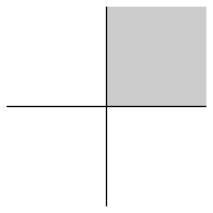
\includegraphics{3_a_subspaces_a.eps}} & \hspace{0.25in} &\begin{minipage}{0.2in} (b) \vspace{1.3in}\end{minipage} &\resizebox{!}{1.5in}{\includegraphics{3_a_subspaces_b.eps}} 
\end{tabular} \\
\begin{tabular}{llcclc} 
\begin{minipage}{0.2in} (c) \vspace{1.4in}\end{minipage} &\resizebox{!}{1.5in}{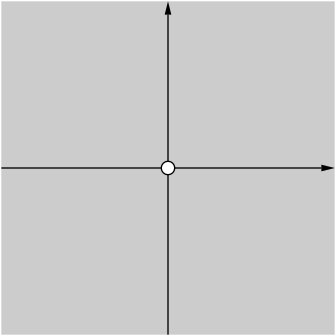
\includegraphics{3_a_subspaces_e.eps}} & \hspace{0.25in} &\begin{minipage}{0.2in} (d) \vspace{1.3in}\end{minipage} &\resizebox{!}{1.5in}{
\includegraphics{3_a_subspaces_g.eps}}
\end{tabular} %\\


\item Determine which of the following sets $W$ is a subspace of $\R^n$ for the indicated value of $n$. Justify your answer.

\ba
\item $W = \{[x \ 0]^{\tr} : x \text{ is a scalar}\}$
\item $W = \{[2x+y \ x-y \ x+y]^{\tr} : x,y \text{ are scalars}\}$
\item $W = \{[x+1 \ x-1]^{\tr} : x \text{ is a scalar}\}$
\item $W = \{[xy \ xz \ yz ]^{\tr} : x,y,z \text{ are scalars}\}$
\ea



\item Find a subset of $\R^2$ that is closed under addition and scalar multiplication, but that does not contain the zero vector, or explain why no such subset exists. 

\item Let $\vv$ be a vector in $\R^2$. What is the smallest subspace of $\R^2$ that contains $\vv$? Explain. Describe this space geometrically. 

\item What is the smallest subspace of $\R^2$ containing the first quadrant? Justify your answer. 

\item Let $\vu$, $\vv$, and $\vw$ be vectors in $\R^3$ with $\vw = \vu+\vv$. Let $W_1 = \Span\{\vu,\vv\}$ and $W_2 = \Span\{\vu,\vv,\vw\}$. 
\ba
\item If $\vx$ is in $W_1$, must $\vx$ be in $W_2$? Explain.

\item If $\vy$ is in $W_2$, must $\vy$ be in $W_1$? Explain.

\item What is the relationship between $\Span\{\vu,\vv\}$ and $\Span\{\vu,\vv,\vw\}$? Be specific. 

\ea

\item Let $m$ and $n$ be positive integers, and let $\vv$ be in $\R^n$. Let $W = \{A\vv : A \in \M_{m \times n}\}$. 
\ba
\item As an example, let $\vv = [2 \ 1]^{\tr}$ in $\R^2$ with $W = \{A\vv : A \in \M_{2 \times 2}\}$. 
	\begin{enumerate}[i.]
	\item Show that the vector $[2 \ 1]^{\tr}$ is in $W$ by finding a matrix $A$ that places $[2 \ 1]^{\tr}$ in $W$.  
	\item Show that the the vector $[4 \ 2]^{\tr}$ is in $W$ by finding a matrix $A$ that places $[4 \ 2]^{\tr}$ in $W$. 
	\item Show that the vector $[6 \ -1]^{\tr}$ is in $W$ by finding a matrix $A$ that places $[6 \ -1]^{\tr}$ in $W$. 
	\item Show that $W = \R^2$. 
	\end{enumerate}
	
\item Show that, regardless of the vector $\vv$ selected, $W$ is a subspace of $\R^m$. 

\item Characterize all of the possibilities for what the subspace $W$ can be. (Hint: There is more than one possibility.)

\ea

\item Let $S_1$ and $S_2$ be subsets of $\R^3$ such that $\Span \ S_1 = \Span \ S_2$. Must it be the case that $S_1$ and $S_2$ contain at least one vector in common? Justify your answer. 

\item Assume $W_1$ and $W_2$ are two subspaces of $\R^n$. Is $W_1 \cap W_2$ also a subspace of $\R^n$? Is $W_1 \cup W_2$ also a subspace of $\R^n$? Justify your answer. (Note: The notation $W_1 \cap W_2$ refers to the vectors common to both $W_1, W_2$, while the notation $W_1 \cup W_2$ refers to the vectors that are in at least one of $W_1, W_2$.)

\item Determine whether the plane defined by the equation $5x+3y-2z=0$ is a subspace in $\R^3$. 

\item If $W$ is a subspace of $\R^n$ and $\vu$ is a vector in $\R^n$ not in $W$, determine whether 
\[ \vu+W = \{\vu+\vv: \vv \text{ is a vector in }W\} \]
is a subspace of $\R^n$.

\item Two students are talking about examples of subspaces. 
\begin{quote}
Student 1: The $x$-axis in $\R^2$ is a subspace. It is generated by the vector $\left[ \begin{array}{c} 1\\0 \end{array}\right]$. 
\end{quote} 
\begin{quote}
Student 2: Similarly $\R^2$ is a subspace of $\R^3$. 
\end{quote} 
\begin{quote}
Student 1: I'm not sure if that will work. Can we fit $\R^2$ inside $\R^3$? Don't we need $W$ to be a subset of $\R^3$ if it is a subspace of $\R^3$?
\end{quote} 
\begin{quote}
Student 2: Of course we can fit $\R^2$ inside $\R^3$. We can think of $\R^2$ as vectors $\left[ \begin{array}{c} a\\b\\0 \end{array} \right]$. That's the $xy$-plane.
\end{quote} 
\begin{quote}
Student 1: I don't know. The vector $\left[ \begin{array}{c} a\\b\\0 \end{array} \right]$ is not exactly same as $\left[ \begin{array}{c} a\\b \end{array} \right]$. 
\end{quote}
\begin{quote}
Student 2: Well, $\R^2$ is a plane and so is the $xy$-plane. So they must be equal, shouldn't they? 
\end{quote} 
\begin{quote}
Student 1: But there are infinitely many planes in $\R^3$. They can't all be equal to $\R^2$. They all ``look like" $\R^2$ but I don't think we can say they are equal.
\end{quote}
Which student is correct? Is $\R^2$ a subspace of $\R^3$, or not? Justify your answer.

\item \label{ex:3_a_sum} Given two subspaces $H_1, H_2$ of $\R^n$, define 
\[ H_1+H_2 = \{ \vw \mid \vw=\vu+\vv \text{ where } \vu \text{ in }H_1, \vv \text{ in }H_2\} \,.\]
Show that $H_1+H_2$ is a subspace of $\R^n$ containing both $H_1, H_2$ as subspaces. The space $H_1+H_2$ is the sum\index{subspace!sum} of the subspaces $H_1$ and $H_2$.

\item Label each of the following statements as True or False. Provide justification for your response.
\ba
\item \textbf{True/False} Any line in $\R^n$ is a subspace in $\R^n$.

\item \textbf{True/False} Any line through the origin in $\R^n$ is a subspace in $\R^n$.

\item \textbf{True/False} Any plane through the origin in $\R^n$ is a subspace in $\R^n$.

\item \textbf{True/False} In $\R^4$, the points satisfying $xy=2t+z$ form a subspace.

\item \textbf{True/False} In $\R^4$, the points satisfying $x+3y=2z$ form a subspace.

\item \textbf{True/False} Any two nonzero vectors generate a plane subspace in $\R^3$.

\item \textbf{True/False} The space $\R^2$ is a subspace of $\R^3$.

\item \textbf{True/False} If $W$ is a subspace of $\R^n$ and $\vu$ is in $W$, then the line through the origin and $\vu$ is in $W$.

\item \textbf{True/False} There are four types of subspaces in $\R^3$: $\{\vzero\}$, line through origin, plane through origin and the whole space $\R^3$.

\item \textbf{True/False} There are four types of subspaces in $\R^4$: $\{\vzero\}$, line through origin, plane through origin and the whole space $\R^4$.

\item \textbf{True/False} The vectors $\left[ \begin{array}{c} 1\\1\\1 \end{array} \right]$, $\left[ \begin{array}{c} 1\\2\\1 \end{array} \right]$ and $\left[ \begin{array}{c} 2\\3\\2 \end{array} \right]$ form a subspace in $\R^3$.

\item \textbf{True/False} The vectors $\left[ \begin{array}{c} 1\\1\\1 \end{array} \right]$ and $\left[ \begin{array}{c} 1\\2\\1 \end{array} \right]$ form a basis of a subspace in $\R^3$.

\ea
\ee

\csection{Project: Least Squares Linear Approximation}
\label{sec:proj_ls_approx}

We return to the problem of finding the least squares line to fit the GDP-consumption data. We will start our work in a more general setting, determining the  method for fitting a linear function to fit any data set, like the GDP-consumption data, in the least squares sense. Then we will apply our result to the GDP-consumption data. 

\begin{pactivity} \label{act:ls_no_line} Suppose we want to fit a linear function $p(x) = mx+b$ to our data. For the sake of our argument, let us assume the general case where we have $n$ data points labeled as $(x_1,y_1)$, $(x_2, y_2)$, $(x_3, y_3)$,  $\ldots$, $(x_n, y_n)$. (In the GDP-consumption data $n = 21$.) In the unlikely event that the graph of $p(x)$ actually passes through these data points, then we would have the system of equations
\begin{align}
y_1 &= b + mx_1  \notag  \\
y_2 &= b + mx_2 \notag  \\
y_3 &= b + mx_3 \label{eq:LS_system} \\
\vdots &\hspace{0.39in} \vdots  \notag\\
y_n &= b + mx_n \notag
\end{align}
in the unknowns $b$ and $m$. 
	\ba
	\item As a small example to illustrate, write the system (\ref{eq:LS_system}) using the three points $(x_1,y_1)= (1,2)$, $(x_2,y_2) = (3,4)$, and $(x_3,y_3) = (5,6)$. Identify the unknowns and then write this system in the form $M \va = \vy$. Explicitly identify the matrix $M$ and the the vectors $\va$ and $\vy$.
	
	\item Identify the specific matrix $M$ and the specific vectors $\va$ and $\vy$ using the data in Table \ref{T:GDP_consumption}.  Explain why the system $M \va = \vy$ is inconsistent. (Remember, we are treating consumption as the independent variable and GDP as the dependent variable.) What does the result tell us about the data? 

	
	\ea

\end{pactivity}


Project Activity \ref{act:ls_no_line} shows that the GDP-consumption data does not lie on a line.  So instead of attempting to find coefficients $b$ and $m$ that give a solution to this system, which may be impossible, we instead look for a vector $\va^*$ that provides us with something that is ``close" to a solution.

If we could find $b$ and $m$ that give a solution to the system $M\va = \vy$, then $M\va - \vy$ would be zero. If we can't make $M\va - \vy$ exactly equal to the vector $\vzero$, we could instead try to minimize $M\va-\vy$ in some way. One way is to minimize the length $||M\va-\vy||$ of the vector $M\va - \vy$.

If we minimize the quantity $||M\va-\vy||$, then we will have minimized a function given by a sum of squares. That is, $||M\va-\vy||$ is calculated to be
\begin{equation}
 \sqrt{(b+mx_1-y_1)^2 + (b+mx_2-y_2)^2 + \cdots + (b+mx_n-y_n)^2}. \label{eq:ls_equation}
\end{equation}
This is why the method we will derive is called the method of least squares. This method provides us with a vector ``solution" in a subspace that is related to $M$. We can visualize $||M \va - \vy||$ as in Figure \ref{F:GDP_error}. In this figure the data points are shown along with a linear approximation (not the best for illustrative purposes). The lengths of the vertical line segments are the summands $(b+mx_i-y_i)$ in (\ref{eq:ls_equation}). So we are trying to minimize the sum of the squares of these line segments. 
\begin{figure}[ht]
\begin{center}
\resizebox{!}{2.5in}{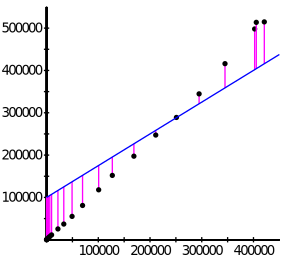
\includegraphics{GDP_error}}
\caption{Error in the linear approximation.}
\label{F:GDP_error}
\end{center}
\end{figure}

Suppose that $\va^*$ minimizes $||M \va - \vy||$. Then the vector $M \va^*$ is the vector that is closest to $\vy$ of all of the vectors of the form $M \vx$. The fact that the vectors of the form $M \vx$ make a subspace will be useful in what follows. We verify that fact in the next project activity.  

\begin{pactivity} \label{act:ls_subspace}  Let $A$ be an arbitrary $m \times k$ matrix. Explain why the set $C = \{A \vx : \vx \in \R^k\}$ is a subspace of $\R^m$. 


\end{pactivity}

Project Activity \ref{act:ls_subspace} shows us that even though the GDP-consumption system $M \va = \vy$ does not have a solution, we can find a vector that is close to a solution in the subspace $\{M \vx : \vx \in \R^2\}$. That is, find a vector $\va^*$ in $\R^{2}$ such that $M \va^*$ is as close (in the least squares sense) to $\vy$ as we can get. In other words, the error $||M \va^* - \vy||$ is as small as possible. In the following activity we see how to find $\va^*$. 

\begin{pactivity} \label{act:ls_minimum} Let 
\[S = \sqrt{(b+mx_1-y_1)^2 + (b+mx_2-y_2)^2 + \cdots + (b+mx_n-y_n)^2},\]
the quantity we want to minimize. The variables in $S$ are $m$ and $b$, so we can think of $S$ as a function of the two independent variables $m$ and $b$. The square root makes calculations more complicated, so it is helpful to notice that $S$ will be a minimum when $S^2$ is a minimum. Since $S^2$ is also function of the two variables $b$ and $m$, the minimum value of $S^2$ will occur when the partial derivatives of $S^2$ with respect to $b$ and $m$ are both $0$ (if you haven't yet taken a multivariable calculus course, you can just assume that this is correct). This yields the equations 
\begin{align}
0 &= \sum_{i=1}^n \left( mx_i + b - y_i\right)x_i  \label{eq:ls_1} \\
0 &= \sum_{i=1}^n \left( mx_i+b-y_i\right). \label{eq:ls_2}
\end{align}
In this activity we solve equations (\ref{eq:ls_1}) and (\ref{eq:ls_2}) for the unknowns $b$ and $m$. (Do this in a general setting without using specific values for the $x_i$ and $y_i$.)
	\ba
	\item Let $r=\sum_{i=1}^n x_i^2$, $s=\sum_{i=1}^n x_i$, $t = \sum_{i=1}^n y_i$, and $u = \sum_{i=1}^n x_iy_i$. Show that the equations (\ref{eq:ls_1}) and (\ref{eq:ls_2}) can be written in the form 
\begin{align*}
0 &= bs + mr -u \\ %\label{eq:revised_1} \\
0 &= bn + ms - t. %\label{eq:revised_2}.
\end{align*}	
Note that this is a system of two linear equations in the unknowns $b$ and $m$.

	\item Write the system from part (a) in matrix form $A \vx = \vb$. Then use techniques from linear algebra to solve the linear system to show that 
\begin{equation} \label{eq:ls_b} 
b = \frac{tr-us}{nr-s^2} = \frac{\left(\sum_{i=1}^n y_i\right) \left(\sum_{i=1}^n x_i^2\right) - \left(\sum_{i=1}^n x_i \right) \left(\sum_{i=1}^n x_iy_i \right)}{n\left(\sum_{i=1}^n x_i^2 \right) - \left(\sum_{i=1}^n x_i \right)^2}
\end{equation}
and
\begin{equation} \label{eq:ls_m} 
m = \frac{nu-ts}{nr-s^2} =  \frac{n\left(\sum_{i=1}^n x_iy_i\right) - \left(\sum_{i=1}^n x_i \right) \left(\sum_{i=1}^n y_i \right)}{n\left(\sum_{i=1}^n x_i^2 \right) - \left(\sum_{i=1}^n x_i \right)^2}.
\end{equation}


\ea

\end{pactivity}
 
\begin{pactivity} Use the formulas (\ref{eq:ls_b}) and (\ref{eq:ls_m}) to find the values of $b$ and $m$ for the regression line to fit the GDP-consumption data in Table \ref{T:GDP_consumption}. You may use the fact that the sum of the GDP data is $3.5164030 \times 10^6$, the sum of the consumption data is $2.9233750 \times 10^6$, the sum of the squares of the consumption data is $8.806564894 \times 10^{11}$, and the sum of the products of the GDP and consumption data is $1.069946378 \times 10^{12}$. Compare to the results the authors obtained in the paper  ``A Statistical Analysis of GDP and Final Consumption Using Simple Linear Regression, the Case of Romania 1990-2010". 



\end{pactivity}



 %12
\achapter{13}{The Null Space and Column Space of a Matrix } \label{sec:null_space}

\vspace*{-17 pt}
\framebox{
\parbox{\dimexpr\linewidth-3\fboxsep-3\fboxrule}
{\begin{fqs}
\item What is the null space of a matrix? 
\item What is the column space of a matrix?
\item What important structure do the null space and column space of a matrix have?
\item What is the kernel of a matrix transformation?
\item How is the kernel of a matrix transformation $T$ defined by $T(\vx) = A\vx$ related to the null space of $A$?
\item What is the range of a matrix transformation?
\item How is the range of a matrix transformation $T$ defined by $T(\vx) = A\vx$ related to the column space of $A$?
\item How do we find a basis for $\Nul A$? 
\item How do we find a basis for $\Col A$? 
\end{fqs}}}% \hspace*{3 pt}}

\vspace*{13 pt}

\csection{Application: The Lights Out Game}

Lights Out (LO) is a commercial game released by Tiger Toys in 1995 (later bought out by Hasbro). The game consists of a $5 \times 5$ grid in which each square is either lit or unlit. Pressing a square changes the status of the square itself and all the squares to the left, right, up, or down. The player's job is to turn all the lights out. You can play a sample game at \url{https://www.geogebra.org/m/wcmctahp}. There is a method to solve any solvable Lights Out game that can be uncovered through linear algebra that we will uncover later in this section. Column spaces and null spaces play important roles in this method. 

\csection{Introduction}

Recall that a subspace of $\R^n$ is a subset of $\R^n$ which is a vector space in itself. More specifically, a subset $W$ or $\R^n$ is a subspace of $\R^n$ if 
\begin{enumerate}
\item whenever $\vu$ and $\vv$ are in $W$ it is also true that $\vu + \vv$ is in $W$ (that is, $W$ is \textbf{closed} under addition),
\item whenever $\vu$ is in $W$ and $a$ is a scalar it is also true that $a\vu$ is in $W$ (that is, $W$ is \textbf{closed} under scalar multiplication),
\item $\vzero$ is in $W$.
\end{enumerate}

Given a matrix $A$, there are several subspaces that are connected to $A$. Two specific such subspaces are the null space of $A$ and the column space of $A$. We will see that these subspaces provide answers to the big questions we have been considering since the beginning of the semester, such as ``Do columns of $A$ span $\R^m$?" ``Are the columns of $A$ linearly independent?" ``Is the transformation $T$ defined by matrix multiplication by $A$ one-to-one?" ``Is the transformation $T$ onto?" 

In this preview activity, we start examining the \emph{null space}. 


\begin{pa} \label{pa:3_b} ~
\be
\item Let $A =  \left[ \begin {array}{ccc} 2&1&3\\ 1&1&4 \end {array} \right]$.
	\ba
	\item Find the general solution to the homogeneous equation $A \vx = \vzero$. Write your solutions in parametric vector form. (Recall that the parametric vector form expresses the solutions to an equation as linear combinations of vectors with free variables as the weights. An example would be $x_3 \left[ \begin{array}{r} 1\\0\\-1\\0\end{array}\right] + x_4 \left[ \begin{array}{r} -2\\1\\0\\1\end{array} \right]$.)



	\item Find two specific solutions $\vx_1$ and $\vx_2$ to the homogeneous equation $A \vx = \vzero$. Is $\vx_1 + \vx_2$ a solution to $A \vx = \vzero$? Explain.



	\item Is $3\vx_1$ a solution to $A \vx = \vzero$? Explain. 



	\item Is $\vzero$ a solution to $A \vx = \vzero$? 
	
	
	
	\item What does the above seem to indicate about the set of solutions to the homogeneous system $A \vx = \vzero$? 



	\ea

\item Let $A$ be an $m \times n$ matrix. As problem 1 implies, the set of solutions to a homogeneous matrix-vector equation $A \vx = \vzero$ appears to be a subspace. We give a special name to this set.



\begin{definition} \label{def:null_space} The \textbf{null space}\index{null space} of an $m \times n$ matrix $A$ is the set of all solutions to $A \vx = \vzero$.
\end{definition}



We denote the null space of a matrix $A$ as $\Nul A$. In set notation we write
\[\Nul A = \{ \vx : A \vx = \vzero\}.\]
Note that since $A\vx=\vzero$ corresponds to a homogeneous system of linear equations, $\Nul A$ also represents the solution set of a homogeneous system.\\

Let $A =  \left[ \begin{array}{cccc} 2&1&3&0\\ 1&1&4&1 \end{array} \right]$. Find all vectors in $\Nul A$. 



\item So far we considered specific examples of null spaces. But what are the properties of a null space in general? Let $A$ be an \emph{arbitrary} $m \times n$ matrix. 
	\ba
	\item The null space of an $m \times n$ matrix is a subset of $\R^k$ for some integer $k$. What is $k$?


	
	\item Now suppose $\vu$ and $\vv$ are two vectors in $\Nul A$. By definition, that means $A\vu=\vzero$, $A\vv=\vzero$. Use properties of the matrix-vector product to show that $\vu + \vv$ is also in $\Nul A$. 



\item Now suppose $\vu$ is a vector in $\Nul A$ and $a$ is a scalar. Explain why $a\vu$ is also in $\Nul A$. 



	\item Explain why $\Nul A$ is a subspace of $\R^n$. 

	\ea
	
\ee
\end{pa}


\csection{The Null Space of a Matrix and the Kernel of a Matrix Transformation}

In this section we explore the \emph{null space} and see how the null space of a matrix is related to the matrix transformation defined by the matrix. 


Let $A$ be an $m \times n$ matrix. In Preview Activity \ref{pa:3_b} we defined the null space of a matrix $A$ (see Definition \ref{def:null_space}) as the set of solutions to the matrix equation $A \vx = \vzero$. Note that the null space of an $m \times n$ matrix is a subset of $\R^n$. We saw that the null space of $A$ is closed under addition and scalar multiplication -- that is, if $\vu$ and $\vv$ are in $\Nul A$ and $a$ and $b$ are any scalars, then $\vu + \vv$ and $a \vu$ are also in $\Nul A$. Since the zero vector is always in $\Nul A$, we can conclude that the null space of $A$ is a subspace of $\R^n$. 



There is a connection between the null space of a matrix and the matrix transformation it defines. Recall that any $m \times n$ matrix $A$ defines a matrix transformation $T$ from $\R^n$ to $\R^m$ by $T(\vx) = A \vx$. The null space of $A$ is then the collection of vectors $\vx$ in $\R^n$ so that $T(\vx) = \vzero$. So if $T$ is a matrix transformation from $\R^n$ to $\R^m$, then the set 
\[\{\vx \text{ in } \R^n : T(\vx) = \vzero\}\]
 is a subspace of $\R^n$ equal to the null space of $A$. This set is is given a special name. 



\begin{definition} Let $T : \R^n \to \R^n$ be a matrix transformation. The \textbf{kernel}\index{kernel} of $T$ is the set
\[\Ker(T) = \{\vx \in \R^n : T(\vx) = \vzero\}.\]
\end{definition}


\begin{activity} \label{act:3_b_1} 
If $T$ is a matrix transformation defined by a matrix $A$, then there is a convenient way to determine if $T$ is one-to-one.
\ba
\item Let $T$ be the matrix transformation defined by $T(\vx) = A\vx$, where 
\[A = \left[ \begin{array}{ccr} 1&2&-1 \\ 0&1&4 \end{array} \right].\]
Find all of the vectors in $\Nul A$. If $\Nul A$ contains more than one vector, can $T$ be one-to-one? Why?


\item Let $T$ be the matrix transformation defined by $T(\vx) = A\vx$, where 
\[A = \left[ \begin{array}{rc} 1&0 \\ 2&1 \\ -1&4 \end{array} \right].\]
Find all of the vectors in $\Nul A$. Is $T$ one-to-one? Why?


\item To find the vectors in the null space of a matrix $A$ we solve the system $A \vx = \vzero$. Since a homogeneous system is always consistent, there are two possibilities for $\Nul A$: either $\Nul A = \{\vzero\}$ or $\Nul A$ contains infinitely many vectors. 
	\begin{enumerate}[i.]
	\item Under what conditions on $A$ is $\Nul A = \{\vzero\}$? What does that mean about $T$ being one-to-one or not? Explain. 

	\item Under what conditions is $\Nul A$ infinite? What does that mean about $T$ being one-to-one or not? Explain.

\item Is is possible for $\Nul A$ to be the whole space $\R^n$? If so, give an example. If not, explain why not.

\end{enumerate}

\ea
\end{activity}


Recall that for a function to be  one-to-one, each output must come from exactly one input. Since a matrix transformation $T$ defined by $T(\vx) = A \vx$ always maps the zero vector to the zero vector, for $T$ to be one-to-one it must be the case that the zero vector is the only vector that $T$ maps to the zero vector. This means that the null space of $A$ must be $\{\vzero\}$. Activity \ref{act:3_b_1} demonstrates that if the matrix $A$ that defines the transformation $T$ has a pivot in every column, then $T(\vx) = \vb$ will have exactly one solution for each $\vb$ in the range of $T$. So a trivial null space is enough to characterize a one-to-one matrix transformation.  


\begin{theorem} \label{thm:3_b_one_to_one_kernel} A matrix transformation $T$ from $\R^n$ to $\R^m$ defined by $T(\vx) = A\vx$ is one-to-one if and only if 
\[\Nul A = \Ker(T) = \{\vzero\}.\] 
\end{theorem}


\csection{The Column Space of a Matrix and the Range of a Matrix Transformation}

Given an $m \times n$ matrix $A$, we have seen that the matrix-vector product $A \vx$ is a linear combination of the columns of $A$ with weights from $\vx$. It follows that the equation $A \vx = \vb$ has a solution if and only if $\vb$ is a linear combination of the columns of $A$. So the span of the columns of $A$ tells us for which vectors the equation $A \vx = \vb$ is consistent. We give the span of the columns of a matrix $A$ a special name. 


\begin{definition} The \textbf{column space}\index{column space} of an $m \times n$ matrix $A$ is the span of the columns of $A$.
\end{definition}


We denote the column space of $A$ as $\Col A$. Given that $A \vx$ is a linear combination of the columns of $A$, we can also write the column space of an $m \times n$ matrix $A$ as
\[\Col A = \{A \vx : \vx \text{ is in } \R^n\}.\]
For the matrix transformation $T$ defined by $T(\vx) = A\vx$, the set of all vectors of the form $A \vx$ is also the range of the transformation $T$. So for a matrix transformation $T$ with matrix $A$ we have $\Range(T) = \Col A$. 

\begin{activity} \label{act:3_b_2} As a span of a set of vectors, we know that $\Col A$ is a subspace of $\R^k$ for an appropriate value of $k$.  
\ba
\item Let $M =  \left[ \begin{array}{ccccr} 1&1&1&0&2 \\ 0&1&0&1&1 \\ 1&0&1&1&-1 \\ 0&1&0&1&1 \end{array} \right]$. 
The space $\Col M$ is a subspace of $\R^k$ for some positive integer $k$. What is $k$ in this case?


\item If $A$ is an $m \times n$ matrix, then $\Col A$ is a subspace of $\R^k$ for some positive integer $k$. What is $k$ in this case?


\item Recall that a matrix transformation $T$ given by $T(\vx)=A\vx$ where $A$ is an $m\times n$ matrix is onto if for every $\vb$ in $\R^m$ there exists a $\vx$ in $\R^n$ for which $T(\vx)=\vb$. How does $T$ being onto relate to the $\Col A$? 


\ea
\end{activity}

As you saw in Activity \ref{act:3_b_2}, a matrix transformation $T$ defined by $T(\vx)=A\vx$ is onto if the column space of $A$, which consists of the image vectors under the transformation $T$, is equal to $\R^m$. In other words, we want the $\Range(T)$ to equal $\R^m$.

\begin{theorem} \label{thm:3_b_onto_range} A matrix transformation $T$ from $\R^n$ to $\R^m$ defined by $T(\vx) = A\vx$ is onto if and only if 
\[\Col A = \Range(T) = \R^m.\] 
\end{theorem}



\csection{The Row Space of a Matrix}

As you might expect, if there is a column space for a matrix then there is also a row space for a matrix. The row space is defined just as the column space as the span of the rows of a matrix. 

\begin{definition} The \textbf{row space}\index{row space} of an $m \times n$ matrix $A$ is the span of the row of $A$.
\end{definition}

There is really nothing new here, though. Since the rows of $A$ are the columns of $A^{\tr}$, it follows that $\Row A = \Col A^{\tr}$. So if we want to learn anything about the row space of $A$, we can just translate all of our questions to the column space of $A^{\tr} $. 

\csection{Bases for $\Nul A$ and $\Col A$}

When confronted with a subspace of $\R^n$, we will usually want to find a minimal spanning set -- a smallest spanning set -- for the space. Recall that a minimal spanning set is also called a basis for the space. So a basis for a space must span that space, and to be a minimal spanning set we have seen that a basis must also be linearly independent.  So to prove that a set is a basis for a subspace of $\R^n$ we need to demonstrate two things: that the set is linearly independent, and that the set spans the subspace. 



\begin{activity} \label{act:3_b_3} In this activity we see how to find a basis for $\Col A$ and $\Nul A$ for a specific matrix $A$. Let 
\[A =  \left[ \begin{array}{rrrrr} 1&1&1&0&2 \\ 0&1&0&1&1 \\ 1&0&1&1&-1 \\ 0&1&0&1&1 \end{array} \right].\] Assume that the reduced row echelon form of $A$ is 
\[R= \left[ \begin{array}{rrrrr} 1&0&1&0&0 \\ 0&1&0&0&2 \\ 0&0&0&1&-1 \\ 0&0&0&0&0\end{array} \right].\] 
\ba 
\item First we examine $\Col A$. Recall that to find a minimal spanning set of a set of vectors $\{\vv_1, \vv_2, \ldots, \vv_k\}$ in $\R^n$ we just select the pivot columns of the matrix $[\vv_1  \ \vv_2  \ \cdots \  \vv_k]$. 
	\begin{enumerate}[i.]
	\item Find a basis for $\Col A$.



	\item Does $\Col A$ equal $\Col R$? Explain.
	


	\end{enumerate}
	
\item Now we look at $\Nul A$. 
	\begin{enumerate}[i.]
	\item Write the general solution to the homogeneous system $A \vx = \vzero$ in vector form. 



	\item Find a spanning set for $\Nul A$. 



	\item Find a basis for $\Nul A$. Explain how you know you have a basis.  



	\end{enumerate}

\ea

\end{activity}


You should have noticed that Activity \ref{act:3_b_3} (a) provides a process for finding a basis for $\Col A$ -- the pivot columns of $A$ form a basis for $\Col A$. Similarly, Activity \ref{act:3_b_3} (b) shows us that we can find a basis for $\Nul A$ by writing the general solution to the homogeneous equation $A\vx = \vzero$ as a linear combination of vectors whose weights are the variables corresponding to the non-pivot columns of $A$ -- and these vectors form a basis for $\Nul A$. As we will argue next, these process always give us bases for $\Col A$ and $\Nul A$. 

Let $A$ be an $m \times n$ matrix, and let $R$ be the reduced row echelon form of $A$. Suppose $R$ has $k$ non-pivot columns and $n-k$ pivot columns. We can rearrange the columns so that the non-pivot columns of $R$ are the last $k$ columns (this just amounts to relabeling the unknowns in the system).

\begin{description}
\item[Basis for $\Nul A$.] Here we argue that the method described following Activity \ref{act:3_b_3} to find a spanning set for the null space always yields a basis for the null space.

First note that $\Nul R = \Nul A$, since the system $A\vx = \vzero$ has the same solution set as $R \vx = \vzero$. So it is enough to find a basis for $\Nul R$. If every column of $R$ is a pivot column, then $R \vx = \vzero$ has only the trivial solution and the null space of $R$ is $\{ \vzero \}$. Let us now consider the case where $R$ contains non-pivot columns. If we let $\vx = [x_1 \ x_2 \ \ldots \ x_n]^{\tr}$, and if $R\vx = \vzero$ then we can write $x_1$, $x_2$, $\ldots$, $x_{n-k}$ in terms of $x_{n-k+1}$, $x_{n-k+2}$, $\ldots$, and $x_n$. From these equations we can write $\vx$ as a linear combination of some vectors $\vv_1$, $\vv_2$, $\ldots$, $\vv_k$ with $x_{n-k+1}$, $x_{n-2+2}$, $\ldots$, $x_n$ as weights. By construction, each of the vectors $\vv_1$, $\vv_2$, $\ldots$, $\vv_k$ has a component that is 1 with the corresponding component as 0 in all the other $\vv_i$. Therefore, the vectors $\vv_1$, $\vv_2$, $\ldots$, $\vv_k$ are linearly independent and span $\Nul R$ (and $\Nul A$). In other words, the method we have developed to find the general solution to $A \vx = \vzero$ always produces a basis for $\Nul A$.
\item[Basis for $\Col A$.] Here we explain why the pivot columns of $A$ form a basis for $\Col A$.  Recall that the product $A \vx$ expresses a linear combination of the columns of $A$ with weights from $\vx$, and every such linear combination is matched with a product $R \vx$ giving a linear combination of the columns of $R$ \emph{using the same weights}. So if a set of columns of $R$ is linearly independent (or dependent), then the set of corresponding columns in $A$ is linearly independent (or dependent) and vice versa. Since each pivot column of $R$ is a vector with 1 in one entry (a different entry for different pivot columns) and zeros elsewhere, the pivot columns of $R$ are clearly linearly independent. It follows that the pivot columns of $A$ are linearly independent. All that remains is to explain why the pivot columns of $A$ span $\Col A$. 

Let $\vr_1$, $\vr_2$, $\ldots$, $\vr_n$ be the columns of $R$ so that $R~=~[\vr_1 \ \ \vr_2 \ \ \cdots \ \ \vr_n]$, and let $\va_1$, $\va_2$, $\ldots$, $\va_n$ be the columns of $A$ so that $A~=~[\va_1 \ \ \va_2 \ \ \cdots \ \ \va_n]$. Suppose $\va_i$ is a non-pivot column for $A$ and $\vr_i$ the corresponding non-pivot column in $R$. Each pivot column is composed of a single 1 with the rest of its entries 0. Also, if a non-pivot column contains a nonzero entry, then there is a corresponding pivot column that contains a 1 in the corresponding position. So $\vr_i$ is a linear combination of $\vr_1$, $\vr_2$, $\ldots$, $\vr_{n-k}$ -- the pivot columns of $R$. Thus,
\[\vr_i = c_1 \vr_1 + c_2\vr_2 + \cdots + c_{n-k}\vr_{n-k}\]
for some scalars $c_1$, $c_2$, $\ldots$, $c_{n-k}$. Let $\vx = [c_1 \ c_2 \ \cdots \ c_{n-k} \ 0 \ \cdots 0 \ -1 \ 0 \ \cdots \ 0]^{\tr}$, where the $-1$ is in position $i$. Then $R \vx = \vzero$ and so $A \vx = \vzero$. Thus, 
\[\va_i = c_1 \va_1 + c_2\va_2 + \cdots + c_{n-k}\va_{n-k}\]
and $\va_i$ is a linear combination of the pivot columns of $A$. So every non-pivot column of $A$ is in the span of $A$ and we conclude that the pivot columns of $A$ form a basis for $\Col A$. 
\end{description}

\noindent \textbf{IMPORTANT POINT:} It is the pivot columns of $A$ that form a basis for $\Col A$, not the pivot columns of the reduced row echelon form $R$ of $A$. In general, $\Col R \neq \Col A$. 

We can incorporate the ideas of this section to expand the Invertible Matrix Theorem.



\begin{theorem}[The Invertible Matrix Theorem] Let $A$ be an $n \times n$ matrix. The following statements are equivalent.
\begin{enumerate}
\item The matrix $A$ is an invertible matrix.
\item \label{item:3_b_trivial_soln} The matrix equation $A \vx = \vzero$ has only the trivial solution.
\item The matrix $A$ has $n$ pivot columns.
\item Every row of $A$ contains a pivot. 
\item The columns of $A$ span $\R^n$.
\item The matrix $A$ is row equivalent to the identity matrix $I_n$.
\item The columns of $A$ are linearly independent.
\item The columns of $A$ form a basis for $\R^n$.
\item The matrix transformation $T$ from $\R^n$ to $\R^n$ defined by $T(\vx) = A\vx$ is one-to-one.
\item The matrix equation $A \vx = \vb$ has exactly one solution for each vector $\vb$ in $\R^n$.
\item The matrix transformation $T$ from $\R^n$ to $\R^n$ defined by $T(\vx) = A\vx$ is onto.
\item \label{item:3_b_AC_I} There is an $n \times n$ matrix $C$ so that $AC = I_n$.
\item \label{item:3_b_DA_I} There is an $n \times n$ matrix $D$ so that $DA = I_n$.
\item The scalar 0 is not an eigenvalue of $A$.
\item The matrix $A^{\tr}$ is invertible.
\item $\Nul A = \{\vzero\}$.
\item $\Col A = \R^n$.
\end{enumerate}
\end{theorem}


\csection{Examples}

\ExampleIntro

\begin{example} ~
\ba
\item Let $A = \left[ \begin{array}{rrrr} 1&0&-2&3 \\ -2&-4&0&-14 \\ 1&3&1&9 \end{array} \right]$.
	\begin{enumerate}[i.]
	\item Find a basis for $\Col A$. 
	
	\item  Describe $\Col A$ geometrically (e.g., as a line, a plane, a union of lines, etc.) in the appropriate larger space. 
	
	\end{enumerate}
	
\item Let $B = \left[ \begin{array}{rrr} 0&-2&1\\-1&0&1 \\ 6&-10&-1 \\ 1&-4&1  \end{array} \right]$.
	\begin{enumerate}[i.]
	\item Find a basis for $\Nul B$. 
	
	\item  Describe $\Nul B$ geometrically (e.g., as a line, a plane, a union of lines, etc.) in the appropriate larger space. 
	
	\end{enumerate}
	
\ea
	
\ExampleSolution
\ba
\item We use $A = \left[ \begin{array}{rrrr} 1&0&-2&3 \\ -2&-4&0&-14 \\ 1&3&1&9 \end{array} \right]$.
	\begin{enumerate}[i.]
	\item Technology shows that the reduced row echelon form of $A$ is 
	\[\left[ \begin {array}{ccrc} 1&0&-2&3\\ 0&1&1&2 \\ 0&0&0&0\end {array} \right].\]
	The first two columns of $A$ are the pivot columns of $A$. Since the pivot columns of $A$ form a basis for $\Col A$, a basis for $\Col A$ is 
	\[\left\{ \left[ \begin {array}{r} 1\\ -2 \\ 1\end {array} \right], \left[ \begin {array}{r} 0\\ -4 \\ 3\end {array} \right] \right\}.\]

	\item Let $\vv_1 =  \left[ \begin {array}{r} 1\\ -2 \\ 1\end {array} \right]$ and $\vv_2 =  \left[ \begin {array}{r} 0\\ -4 \\ 3\end {array} \right]$. Since neither $\vv_1$ nor $\vv_2$ is a scalar multiple of the other, we see that $\Col A$ is the span of two linearly independent vectors in $\R^3$. Thus, we conclude that $\Col A$ is the plane in $\R^3$ through the origin and the points $(1,-2,1)$ and $(0,-4,3)$. 
	
	\end{enumerate}
	
\item We use $B = \left[ \begin{array}{rrr} 0&-2&1\\-1&0&1 \\ 6&-10&-1 \\ 1&-4&1  \end{array} \right]$.
	\begin{enumerate}[i.]
	\item Technology shows that the reduced row echelon form of $B$ is 
	\[\left[ \renewcommand{\arraystretch}{1.5} \begin {array}{ccr} 1&0&-1\\ 0&1&-\frac{1}{2} \\ 0&0&0 \\ 0&0&0\end {array} \right].\]
	To find a basis for $\Nul B$, we must solve the homogeneous equation $B \vx = \vzero$. If $\vx = \left[ \begin{array}{c}x_1\\x_2\\x_3 \end{array} \right]$ and $B \vx = \vzero$, the reduced row echelon form of $B$ shows that $x_3$ is free, $x_2 = \frac{1}{2}x_3$, and $x_1 = x_3$. So 
	\begin{align*}
	\vx &= \left[ \begin{array}{c}x_1\\x_2\\x_3 \end{array} \right] \\
		&= \left[ \renewcommand{\arraystretch}{1.5} \begin{array}{c}x_3\\ \frac{1}{2}x_3 \\x_3 \end{array} \right] \\
		&= x_3\left[ \renewcommand{\arraystretch}{1.5} \begin{array}{c}1\\ \frac{1}{2}1\\1 \end{array} \right] .
	\end{align*}
	 Thus, a basis for $\Nul B$ is 
	\[\left\{ \left[ \begin {array}{c} 2\\ 1 \\ 2\end {array} \right] \right\}.\]

	\item  Since $\Nul B = \Span\left\{ \left[ \begin {array}{c} 2\\ 1 \\ 2\end {array} \right] \right\}$ is the span of one nonzero vector in $\R^3$, we conclude that $\Nul B$ is the line in $\R^3$ through the origin and the point $(2,1,2)$.
	\end{enumerate}
	
\ea


\end{example}


\begin{example} Let $A = \left[ \begin{array}{rr} 1&3\\-1&2 \\ 0&-2\\5&6 \end{array} \right]$, and let $T$ be the matrix transformation defined by $T(\vx) = A\vx$.
\ba
\item What are the domain and codomain of $T$? Why? 

\item Find all vectors $\vx$ such that $T(\vx) = \vzero$. How is this set of vectors related to $\Nul A$? Explain.

\item Is $T$ one-to-one? Explain.

\item Is $T$ onto? If yes, explain why. If no, find a basis for the range of $T$. 

\ea

\ExampleSolution

\ba
\item Recall that $A \vx$ is a linear combination of the columns of $A$ with weights from $\vx$. So $A \vx$ is defined only when the number of components of $\vx$ is equal to the number of columns of $A$. This explains why the domain of $T$ is $\R^2$. Also, since each output of $T$ is a linear combination of the columns of $A$, the codomain of $T$ is $\R^4$. 

\item The set of vectors $\vx$ such that $\vzero = T(\vx) = A\vx$ is the same as $\Nul A$. The reduced row echelon form of $A$ is 
\[\left[ \begin{array}{cc} 1&0\\0&1\\0&0\\0&0 \end{array}\right].\]
Since both columns of $A$ are pivot columns, the columns of $A$ are linearly independent. This implies that $A \vx = \vzero$ has only the trivial solution. Therefore, the only vector $\vx$ such that $T(\vx) = \vzero$ is the zero vector in $\R^2$. 

\item The previous part shows that $\Ker(T) = \{\vzero\}$. This means that $T$ is one-to-one by Theorem \ref{thm:3_b_one_to_one_kernel}. 

\item Recall that the range of $T$ is the same as $\Col A$. The reduced row echelon form of $A$ has a row of zeros, so $A \vx = \vb$ is not consistent for every $\vb$ in $\R^4$. We conclude that $T$ is not onto. To find a basis for the range of $T$, we just need to find a basis for $\Col A$. The pivot columns of $A$ form such a basis, so a basis for the range of $T$ is 
\[\left\{ \left[ \begin{array}{r} 1\\-1 \\ 0\\5 \end{array} \right], \left[ \begin{array}{r} 3\\2 \\ -2\\6 \end{array} \right] \right\}.\]

\ea

\end{example}

\csection{Summary}

\begin{itemize}
\item The null space of an $m \times n$ matrix $A$ is the set of vectors $\vx$ in $\R^n$ so that $A \vx = \vzero$. In set notation
\[\Nul A = \{\vx : A \vx = \vzero\}.\]
\item The column space of a matrix $A$ is the span of the columns of $A$.
\item A subset $W$ of $\R^n$ is a subspace of $\R^n$ if
\begin{enumerate}
\item $\vu + \vv$ is in $W$ whenever $\vu$ and $\vv$ are in $W$ (when this property is satisfied we say that $W$ is \emph{closed} under addition),
\item $a \vu$ is in $W$ whenever $a$ is a scalar and $\vu$ is in $W$ (when this property is satisfied we say that $W$ is \emph{closed} under multiplication by scalars),
\item $\vzero$ is in $W$.
\end{enumerate}
\item The null space of an $m \times n$ matrix is a subspace of $\R^n$ while the column space of $A$ is a subspace of $\R^m$.
\item The span of any set of vectors in $\R^n$ is a subspace of $\R^n$. 
\item The kernel of a matrix transformation $T : \R^n \to \R^m$ is the set 
\[\Ker(T) = \{\vx \in \R^n : T(\vx) = \vzero\}.\]
\item The kernel of a matrix transformation $T$ defined by $T(\vx) = A\vx$ is the same set as $\Nul A$. 
\item The range of a matrix transformation $T : \R^n \to \R^m$ is the set 
\[\Range(T) = \{T(\vx) : \vx \in \R^n\}.\]
\item The range of a matrix transformation $T$ defined by $T(\vx) = A\vx$ is the same set as $\Col A$. 
\item A basis for the null space of a matrix $A$ can be found by writing the general solution to the homogeneous equation $A \vx = \vzero$ as a linear combination of vectors whose weights are the variables corresponding to the non-pivot columns of $A$. The number of vectors in a basis for $\Nul A$ is the number of non-pivot columns of $A$.
\item The pivot columns of a matrix $A$ form a basis for the column space of $A$.
\end{itemize}



\csection{Exercises}
\be
\item Find a basis for the null space and column space of the matrix 
\[A=\left[ \begin{array}{cccr} 1 & 2& 3& 4\\ 0 & 0 & 2 & -2 \\ 1 & 2 & 5 & 2 \end{array} \right].\]
Of which spaces are the null and column spaces of $A$ subspaces?

\item If the column space of $\left[ \begin{array}{ccr} 1&2&-1\\1&1&1\\1&2&c\end{array} \right]$ has basis $\left\{ \left[ \begin{array}{c} 1\\1\\1 \end{array} \right], \left[ \begin{array}{c} 2\\1\\2 \end{array} \right]\right\}$, what must $c$ be?

\item If the null space of $\left[ \begin{array}{ccc} 2&1&a\\ 1&2&b \end{array} \right]$ has basis $\left\{ \left[ \begin{array}{r} 2\\-1\\1 \end{array} \right]\right\}$, what must $a$ and $b$ be?

\item Find a matrix with at least four non-zero and distinct columns for which the column space has basis $\left\{ \left[ \begin{array}{c} 1\\1\\1\end{array} \right] , \left[ \begin{array}{c} 2\\2\\3\end{array} \right] \right\}$.

\item Find a matrix with at least two rows whose null space has basis $\left\{ \left[ \begin{array}{r} 1\\1\\-1\end{array} \right] \right\}$.

\item Find a matrix whose column space has basis $\left\{ \left[ \begin{array}{c} 1\\1\\1\end{array} \right] , \left[ \begin{array}{c} 2\\2\\3\end{array} \right] \right\}$ and whose null space has basis $\left\{ \left[ \begin{array}{r} 2\\1\\-1\end{array} \right] \right\}$.

\item If possible, find a $4\times 4$ matrix whose column space does not equal $\R^4$ but whose null space equals $\{\vzero\}$. Explain your answer. If not possible, explain why not.

\item Label each of the following statements as True or False. Provide justification for your response.
\ba
\item \textbf{True/False} For a $3\times 4$ matrix, the null space contains vectors other than the zero vector.

\item \textbf{True/False} For a $4\times 3$ matrix, the null space contains vectors other than the zero vector.

\item \textbf{True/False} If Nul $A$ is not the zero subspace, then the transformation ${\bf x} \mapsto A{\bf x}$ is not one-to-one.

\item \textbf{True/False} If the transformation ${\bf x} \mapsto A{\bf x}$ is onto where $A$ is an $m\times n$ matrix, then Col $A=\R^m$.

\item \textbf{True/False} For a $4\times 3$ matrix $A$, Col $A$ cannot equal $\R^4$.

\item \textbf{True/False} For a $3\times 4$ matrix $A$, Col $A$ cannot equal $\R^3$.

\item \textbf{True/False} The null space of the matrix $\begin{bmatrix} 1 & 1 & 1 \\1 & 1 & 1 \\ 1 & 1 & 1\end{bmatrix}$ consists of the two vectors $[-1 \ 0 \ 1]^{\tr}$ and $[0 \ -1 \ 1]^{\tr}$.

\item \textbf{True/False} A basis for the null space of the matrix $\begin{bmatrix} 1 & 1 & 1 \\1 & 1 & 1 \\ 1 & 1 & 1\end{bmatrix}$ consists of the two vectors $[-1 \ 0 \ 1]^{\tr}$ and $[0 \ -1 \ 1]^{\tr}$.

\item \textbf{True/False} There does not exist a matrix whose null space equals its column space.

\item \textbf{True/False} The column space of every $4\times 4$ matrix is $\R^4$ and its null space is $\{\vzero\}$.

\ea

\ee

\csection{Project: Solving the Lights Out Game}
The Lights Out game starts with a $5 \times 5$ grid on which some of the squares are lit (on) and some are not lit (off). We will call such a state a \emph{configuration}. Pressing a square that is on turns it off and changes the state of all adjacent (vertically and horizontally) squares, and pressing a square that is off turns it on and changes the state of all adjacent (vertically and horizontally) squares. To model this situation, we consider the number system $\Z_2 = \{0,1\}$ consisting only of 0 and 1, where 0 represents the off state and 1 the on state. We can also think of 1 as the act of pressing a square and 0 as the act of not pressing -- that is,
\begin{itemize}
\item $0+0 = 0$ (not pressing an off square leaves it off),
\item $0+1 = 1 = 1 + 0$ (pressing an off square turns it on or not pressing a lit square leaves it lit),
\item $1+1 = 0$ (pressing a lit square turns it off).
\end{itemize}

The numbers 0 and 1 in $\Z_2$ will be the only numbers we use when playing the Lights Out game, so all of our matrix entries will be in $\Z_2$ and all of our calculations are done in $\Z_2$. 

There are two ways we can view a Lights Out game.
\begin{itemize}
\item We can view each configuration as a $5 \times 5$ matrix. In this situation, we label the entries in the grid as shown in Figure \ref{F:LO}. Each entry in the grid will be assigned a 0 or 1 according to whether the light in that entry is off or on.

\item For our purposes a better way to visualize a Lights Out configuration is as a $25 \times 1$ vector. The components in this vector correspond to the entries in the $5 \times 5$ grid with the correspondence given by the numbering demonstrated in Figure \ref{F:LO} (for the sake of space, this array is shown in a row instead of a column). Again, each component is assigned a 0 or 1 according to whether the light for that entry is off or on. In this view, each configuration is a vector with 25 components in $\Z_2$.
\end{itemize}

\begin{figure}[h]
\begin{center}

\resizebox{!}{1.0in}{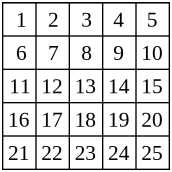
\includegraphics{LO}} \\

\vspace{6pt}

\resizebox{!}{0.22in}{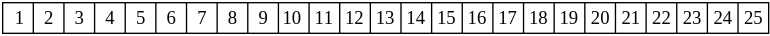
\includegraphics{LO_vector}}

\end{center}
\caption{Two representations of the Lights Out game.}
\label{F:LO}
\end{figure}

We will take the latter perspective and view the Lights Out game as if it is played on a $25 \times 1$ board with entries in $\Z_2$. The space of all of these Lights Out configurations is denoted as $\Z_2^{25}$ (similar to $\R^{25}$, but with entries in $\Z_2$ rather than $\R$). Since $\Z_2$ is a field, the space $\Z_2^{25}$ is a vector space just as $\R^{25}$ is. This is the environment in which we will play the Lights Out game.

If we think about the game as played on a $25 \times 1$ board, then pressing a square correlates to selecting one of the 25 components of a configuration vector. Each time we press a square, we make a move that changes the status of that square and all the squares vertically or horizontally adjacent to it from the $5 \times 5$ board. Recalling that adding 1 to a square has the effect of changing its status (from on to off or off to on), and each move that we make in the game can be represented as a $25 \times 1$ vector that is added to a configuration. For example, the move of pressing the first square is given by adding the vector
\[\vm_{1} = [ 1 \ 1 \ 0 \ 0 \ 0 \ 1 \ 0 \ 0 \ 0 \ 0 \ 0 \ 0 \ 0 \ 0 \ 0 \ 0 \ 0 \ 0 \ 0 \ 0\  0 \ 0 \ 0 \ 0 \ 0 ]^{\tr}\]
to a configuration vector and the move of pressing the second square is represented by adding the vector 
\[\vm_{2} = [ 1 \ 1 \ 1 \ 0 \ 0 \ 0 \ 1 \ 0 \ 0 \ 0 \ 0 \ 0 \ 0 \ 0 \ 0 \ 0 \ 0 \ 0 \ 0 \ 0\  0 \ 0 \ 0 \ 0 \ 0 ]^{\tr}.\]



\begin{pactivity} Let $\vm_i$ be the move of pressing the $i$th square for $i$ from 1 to 25. 
\ba
\item Find vector representations for $\vm_9$ and $\vm_{22}$. %each of the other 23 moves


\item Let $M = [m_{ij}] =  \left[\vm_1 | \vm_2 | \cdots | \vm_{25} \right]$. Explain why $m_{ij} = m_{ji}$ for each $i$ and $j$. In other words, explain why $M^{\tr} = M$. (Such a matrix is called a \emph{symmetric} matrix.)


\ea

\end{pactivity}

The goal of the Lights Out game is to begin with an initial configuration $\vc$ (a vector in $\Z_2^{25}$) and determine if we can apply a sequence of moves to obtain the configuration in which all the entries are 0 (or all the lights are off). The vector in $\Z_2^{25}$ of all 0s is the zero vector in $\Z_2^{25}$ and we will denote it as $\vzero$. Some basic algebra of vector addition in $\Z_2$ (or mod 2) will help us understand the strategy.

Start with a configuration $\vc$. If we press the $i$th square, then we obtain the new configuration $\vc_1 = \vm_i + \vc$ (where each move $\vm_i$ is also in $\Z_2^{25}$).

\begin{pactivity} \label{act_LO_1} ~
\ba
\item What happens if we press the $i$th square twice in a row? Explain in terms of the action and the game and verify using vector addition.


\item Explain why applying move $\vm_i$ then move $\vm_j$ is the same as applying move $\vm_j$, then $\vm_i$.


\item Explain how the answers to the previous two questions show that to play the game we only need to determine which buttons to press (and only once each) without worrying about the order in which the buttons are pressed.


\ea

\end{pactivity}



What we have seen is that to play the game we are really looking for scalars $x_1$, $x_2$, $\ldots$, $x_{25}$ in $\Z_2$ (in other words, either 0 or 1) so that
\begin{equation}
x_1\vm_1 + x_2\vm_2 + \cdots + x_{25}\vm_{25} + \vc = \vzero. \label{eq:LO1}
\end{equation}



\begin{pactivity} Explain why (\ref{eq:LO1}) has the equivalent matrix equation
\begin{equation}
M\vx = \vc, \label{eq:LO2}
\end{equation}
where $M = \left[\vm_1 | \vm_2 | \cdots | \vm_{25} \right]$, or 
\[M =
\arraycolsep=3.0pt
\left[ \begin{array}{c c c c c c c c c c c c c c c c c c c c c c c c c }
1 & 1 & 0 & 0 & 0 & 1 & 0 & 0 & 0 & 0 & 0 & 0 & 0 & 0 & 0 & 0 & 0 & 0 & 0 & 0 & 0 & 0 & 0 & 0 & 0 \\
1 & 1 & 1 & 0 & 0 & 0 & 1 & 0 & 0 & 0 & 0 & 0 & 0 & 0 & 0 & 0 & 0 & 0 & 0 & 0 & 0 & 0 & 0 & 0 & 0 \\
0 & 1 & 1 & 1 & 0 & 0 & 0 & 1 & 0 & 0 & 0 & 0 & 0 & 0 & 0 & 0 & 0 & 0 & 0 & 0 & 0 & 0 & 0 & 0 & 0 \\
0 & 0 & 1 & 1 & 1 & 0 & 0 & 0 & 1 & 0 & 0 & 0 & 0 & 0 & 0 & 0 & 0 & 0 & 0 & 0 & 0 & 0 & 0 & 0 & 0 \\
0 & 0 & 0 & 1 & 1 & 0 & 0 & 0 & 0 & 1 & 0 & 0 & 0 & 0 & 0 & 0 & 0 & 0 & 0 & 0 & 0 & 0 & 0 & 0 & 0 \\
1 & 0 & 0 & 0 & 0 & 1 & 1 & 0 & 0 & 0 & 1 & 0 & 0 & 0 & 0 & 0 & 0 & 0 & 0 & 0 & 0 & 0 & 0 & 0 & 0 \\
0 & 1 & 0 & 0 & 0 & 1 & 1 & 1 & 0 & 0 & 0 & 1 & 0 & 0 & 0 & 0 & 0 & 0 & 0 & 0 & 0 & 0 & 0 & 0 & 0 \\
0 & 0 & 1 & 0 & 0 & 0 & 1 & 1 & 1 & 0 & 0 & 0 & 1 & 0 & 0 & 0 & 0 & 0 & 0 & 0 & 0 & 0 & 0 & 0 & 0 \\
0 & 0 & 0 & 1 & 0 & 0 & 0 & 1 & 1 & 1 & 0 & 0 & 0 & 1 & 0 & 0 & 0 & 0 & 0 & 0 & 0 & 0 & 0 & 0 & 0 \\
0 & 0 & 0 & 0 & 1 & 0 & 0 & 0 & 1 & 1 & 0 & 0 & 0 & 0 & 1 & 0 & 0 & 0 & 0 & 0 & 0 & 0 & 0 & 0 & 0 \\
0 & 0 & 0 & 0 & 0 & 1 & 0 & 0 & 0 & 0 & 1 & 1 & 0 & 0 & 0 & 1 & 0 & 0 & 0 & 0 & 0 & 0 & 0 & 0 & 0 \\
0 & 0 & 0 & 0 & 0 & 0 & 1 & 0 & 0 & 0 & 1 & 1 & 1 & 0 & 0 & 0 & 1 & 0 & 0 & 0 & 0 & 0 & 0 & 0 & 0 \\
0 & 0 & 0 & 0 & 0 & 0 & 0 & 1 & 0 & 0 & 0 & 1 & 1 & 1 & 0 & 0 & 0 & 1 & 0 & 0 & 0 & 0 & 0 & 0 & 0 \\
0 & 0 & 0 & 0 & 0 & 0 & 0 & 0 & 1 & 0 & 0 & 0 & 1 & 1 & 1 & 0 & 0 & 0 & 1 & 0 & 0 & 0 & 0 & 0 & 0 \\
0 & 0 & 0 & 0 & 0 & 0 & 0 & 0 & 0 & 1 & 0 & 0 & 0 & 1 & 1 & 0 & 0 & 0 & 0 & 1 & 0 & 0 & 0 & 0 & 0 \\
0 & 0 & 0 & 0 & 0 & 0 & 0 & 0 & 0 & 0 & 1 & 0 & 0 & 0 & 0 & 1 & 1 & 0 & 0 & 0 & 1 & 0 & 0 & 0 & 0 \\
0 & 0 & 0 & 0 & 0 & 0 & 0 & 0 & 0 & 0 & 0 & 1 & 0 & 0 & 0 & 1 & 1 & 1 & 0 & 0 & 0 & 1 & 0 & 0 & 0 \\
0 & 0 & 0 & 0 & 0 & 0 & 0 & 0 & 0 & 0 & 0 & 0 & 1 & 0 & 0 & 0 & 1 & 1 & 1 & 0 & 0 & 0 & 1 & 0 & 0 \\
0 & 0 & 0 & 0 & 0 & 0 & 0 & 0 & 0 & 0 & 0 & 0 & 0 & 1 & 0 & 0 & 0 & 1 & 1 & 1 & 0 & 0 & 0 & 1 & 0 \\
0 & 0 & 0 & 0 & 0 & 0 & 0 & 0 & 0 & 0 & 0 & 0 & 0 & 0 & 1 & 0 & 0 & 0 & 1 & 1 & 0 & 0 & 0 & 0 & 1 \\
0 & 0 & 0 & 0 & 0 & 0 & 0 & 0 & 0 & 0 & 0 & 0 & 0 & 0 & 0 & 1 & 0 & 0 & 0 & 0 & 1 & 1 & 0 & 0 & 0 \\
0 & 0 & 0 & 0 & 0 & 0 & 0 & 0 & 0 & 0 & 0 & 0 & 0 & 0 & 0 & 0 & 1 & 0 & 0 & 0 & 1 & 1 & 1 & 0 & 0 \\
0 & 0 & 0 & 0 & 0 & 0 & 0 & 0 & 0 & 0 & 0 & 0 & 0 & 0 & 0 & 0 & 0 & 1 & 0 & 0 & 0 & 1 & 1 & 1 & 0 \\
0 & 0 & 0 & 0 & 0 & 0 & 0 & 0 & 0 & 0 & 0 & 0 & 0 & 0 & 0 & 0 & 0 & 0 & 1 & 0 & 0 & 0 & 1 & 1 & 1 \\
0 & 0 & 0 & 0 & 0 & 0 & 0 & 0 & 0 & 0 & 0 & 0 & 0 & 0 & 0 & 0 & 0 & 0 & 0 & 1 & 0 & 0 & 0 & 1 & 1 \\
\end{array}\right].\]
Explicitly identify the vector $\vx$. Also, explain why $\vc$ is on the right side of this equation. 


\end{pactivity}


To solve a Lights Out game now, all we need do is determine a solution, if one exists, to the matrix equation (\ref{eq:LO2}). 
\begin{pactivity} \label{act:LO_2} For this activity you may use the fact that the reduced row echelon form of the matrix $M$ (using algebra in $\Z_2$) is as shown below. 
\ba
\item Find a basis for the column space of $M$. 

\item Explain why not every Lights Out puzzle can be solved. That is, explain why there are some initial configurations of lights on and off for which it is not possible to turn out all the lights (without turning off the game). Relate this to the column space of $M$.


\ea

\end{pactivity}

 The reduced row echelon form of the matrix $M$ (using algebra in $\Z_2$):
\[ \arraycolsep=3pt \left[ \begin {array}{ccccccccccccccccccccccccc}
1&0&0&0&0&0&0&0&0&0&0&0&0&0&0&0&0&0&0&0&0&0&0&0&1 \\
0&1&0&0&0&0&0&0&0&0&0&0&0&0&0&0&0&0&0&0&0&0&0&1&0 \\
0&0&1&0&0&0&0&0&0&0&0&0&0&0&0&0&0&0&0&0&0&0&0&1&1 \\
0&0&0&1&0&0&0&0&0&0&0&0&0&0&0&0&0&0&0&0&0&0&0&1&0 \\
0&0&0&0&1&0&0&0&0&0&0&0&0&0&0&0&0&0&0&0&0&0&0&0&1 \\
0&0&0&0&0&1&0&0&0&0&0&0&0&0&0&0&0&0&0&0&0&0&0&1&1 \\
0&0&0&0&0&0&1&0&0&0&0&0&0&0&0&0&0&0&0&0&0&0&0&0&0 \\
0&0&0&0&0&0&0&1&0&0&0&0&0&0&0&0&0&0&0&0&0&0&0&1&1 \\
0&0&0&0&0&0&0&0&1&0&0&0&0&0&0&0&0&0&0&0&0&0&0&0&0 \\
0&0&0&0&0&0&0&0&0&1&0&0&0&0&0&0&0&0&0&0&0&0&0&1&1 \\
0&0&0&0&0&0&0&0&0&0&1&0&0&0&0&0&0&0&0&0&0&0&0&1&0 \\
0&0&0&0&0&0&0&0&0&0&0&1&0&0&0&0&0&0&0&0&0&0&0&1&0 \\
0&0&0&0&0&0&0&0&0&0&0&0&1&0&0&0&0&0&0&0&0&0&0&0&0 \\
0&0&0&0&0&0&0&0&0&0&0&0&0&1&0&0&0&0&0&0&0&0&0&1&0 \\
0&0&0&0&0&0&0&0&0&0&0&0&0&0&1&0&0&0&0&0&0&0&0&1&0 \\
0&0&0&0&0&0&0&0&0&0&0&0&0&0&0&1&0&0&0&0&0&0&0&1&1 \\
0&0&0&0&0&0&0&0&0&0&0&0&0&0&0&0&1&0&0&0&0&0&0&0&0 \\
0&0&0&0&0&0&0&0&0&0&0&0&0&0&0&0&0&1&0&0&0&0&0&1&1 \\
0&0&0&0&0&0&0&0&0&0&0&0&0&0&0&0&0&0&1&0&0&0&0&0&0 \\
0&0&0&0&0&0&0&0&0&0&0&0&0&0&0&0&0&0&0&1&0&0&0&1&1 \\
0&0&0&0&0&0&0&0&0&0&0&0&0&0&0&0&0&0&0&0&1&0&0&0&1 \\
0&0&0&0&0&0&0&0&0&0&0&0&0&0&0&0&0&0&0&0&0&1&0&1&0 \\
0&0&0&0&0&0&0&0&0&0&0&0&0&0&0&0&0&0&0&0&0&0&1&1&1 \\
0&0&0&0&0&0&0&0&0&0&0&0&0&0&0&0&0&0&0&0&0&0&0&0&0 \\
0&0&0&0&0&0&0&0&0&0&0&0&0&0&0&0&0&0&0&0&0&0&0&0&0
\end {array} \right].\]


To find conditions under which a Lights Out game is not solvable, we will demonstrate that  if $A$ is an $n \times n$ matrix, then the scalar product of any vector in $\Nul A^{\tr}$ with any column of $A$ is $\vzero$. Let $A = [a_{ij}]$ be an $n \times n$ matrix with columns $\va_1$, $\va_2$, $\ldots$, $\va_n$. Represent the entries in the $i$th column as  $\va_i = [a_{1i} \ a_{2i} \ \ldots \ a_{ni}]^{\tr}$ for each $i$ between 1 and $n$. Note that $\va_i$ is also the $i$th row of $A^{\tr}$. Also, let $\vx = [x_1 \ x_2 \ \ldots \ x_n]^{\tr}$ be a vector in $\Nul A^{\tr}$. Then $A^{\tr} \vx = \vzero$. Using the row-column method of multiplying a matrix by a vector, when we multiply the $i$th row of $A^{\tr}$ with $\vx$ we obtain
    \begin{equation}
    a_{1i}x_1 + a_{2i}x_2 + \cdots + a_{ni}x_n = 0. \label{eq:LO_dp}
    \end{equation}
    This equation is valid for each $i$ between 1 and $n$. Recall that the sum in (\ref{eq:LO_dp}) is the scalar product of $\va_i$ and $\vx$ and is denoted  $\va_i \cdot \vx$. That is,
     \[\va_i \cdot \vx = a_{i1}x_1 + a_{i2}x_2 + \cdots + a_{in}x_n.\]
     The fact that $\vx$ is in $\Nul A^{\tr}$ means $\va_i \cdot \vx = \vzero$ for every $i$ between 1 and $n$. In other words, the scalar product of any vector in $\Nul A^{\tr}$ with any column of $A$ is $\vzero$. (When the scalar product of two vectors is $\vzero$, we call the vectors \emph{orthogonal} -- a fancy word for ``perpendicular".) Since scalar products are linear, we can extend this result to the following.
     
 \begin{theorem} \label{thm:LO_Nul_Col} Let $A$ be an $n \times n$ matrix. If $\vx$ is any vector in $\Col A$ and $\vy$ is any vector in $\Nul A^{\tr}$, then $\vx \cdot \vy = 0$. 
\end{theorem}
     
With Theorem \ref{thm:LO_Nul_Col} in mind we can return to our analysis of the Lights Out game, applying this result to the matrix $M$. 

\begin{pactivity} ~
\ba
\item Find a basis for the null space of $M^{\tr}$. (Recall that $M^{\tr} = M$, so you can use the reduced row echelon form of $M$ (using algebra in $\Z_2$) given earlier.) 



\item Use  Theorem \ref{thm:LO_Nul_Col}  to show that if $\vc = [c_1 \  c_2 \  \ldots \  c_{25}]^{\tr}$ is an initial Lights Out configuration that is solvable, then $\vc$ must be orthogonal to each of the vectors in a basis for $\Nul M^{\tr}$. Then show that if $\vc$ is a solvable initial Lights Out configuration, $\vc$ must satisfy
\begin{align*}
c_2 + c_3 + c_4 + c_6 + c_8 + c_{10} + c_{11} + c_{12} &+ c_{14} + c_{15} + c_{16} + c_{18}  \\
	&+ c_{20} + c_{22} + c_{23} + c_{24} = 0 
\end{align*}
and
\begin{equation*}
c_1 + c_3 + c_5 + c_6 + c_8 + c_{10} + c_{16} + c_{18} + c_{20} + c_{21} + c_{23} + c_{25} = 0.
\end{equation*}
Be very specific in your explanation.


\ea
\end{pactivity}



\begin{pactivity} Now that we know which Lights Out games can be solved, let $\vc$ be an initial configuration to a solvable Lights Out game. Explain how to find a solution to this game. Will the solution be unique? Explain.
\end{pactivity}


Now that we have a strategy for solving the Lights Out game, use it to solve random puzzles at \url{https://www.geogebra.org/m/wcmctahp}, or create your own game to solve. 





  %13
\achapter{14}{Eigenspaces of a Matrix} \label{sec:eigenspaces}

\vspace*{-17 pt}
\framebox{
\parbox{\dimexpr\linewidth-3\fboxsep-3\fboxrule}
{\begin{fqs}
\item What is an eigenspace of a matrix?
\item How do we find a basis for an eigenspace of a matrix?
\item What is true about any set of eigenvectors for a matrix that correspond to different eigenvalues? 
\end{fqs}}}% \hspace*{3 pt}}

\vspace*{13 pt}

\csection{Application: Population Dynamics}

The study of population dynamics -- how and why people move from one place to another -- is important to economists. The movement of people corresponds to the movement of money, and money makes the economy go. As an example, we might consider a simple model of population migration to and from the state of Michigan.

According to the Michigan Department of Technology, Management, and Budget,\footnote{\url{http://michigan.gov/cgi/0,1607,7-158-54534-140915--,00.html}} from 2011 to 2012, approximately 0.05\% of the U.S. population outside of Michigan moved to the state of Michigan, while approximately 2\% of Michigan's population moved out of Michigan. A reasonable question to ask about this situation is, if these numbers don't change, what is the long-term distribution of the US population inside and outside of Michigan (under the assumption that the total US population doesn't change.). The answer to this question involves eigenvalues and eigenvectors of a matrix. More details can be found later in this section. 


\csection{Introduction}



\begin{pa} \label{pa:3_c_1} Consider the matrix transformation $T$ from $\R^2$ to $\R^2$ defined by $T(\vx) = A \vx$, where
\[A = \left[ \begin{array}{cc} 3&1\\1&3 \end{array} \right].\]
We are interested in understanding what this matrix transformation does to vectors in $\R^2$.  The matrix $A$ has eigenvalues $\lambda_1 = 2$ and $\lambda_2 = 4$ with corresponding eigenvectors $\vv_1 = \left[ \begin{array}{r} -1\\1 \end{array} \right]$ and $\vv_2 = \left[ \begin{array}{c} 1\\1 \end{array} \right]$. 

\be
\item Explain why $\vv_1$ and $\vv_2$ are linearly independent.


\item  Explain why any vector $\vb$ in $\R^2$ can be written uniquely as a linear combination of $\vv_1$ and $\vv_2$. 

\item We now consider the action of the matrix transformation $T$ on a linear combination of $\vv_1$ and $\vv_2$. Explain why 
\begin{equation} \label{eq:3_c_1}
T(c_1\vv_1 + c_2 \vv_2) = 2c_1\vv_1 + 4c_2 \vv_2. 
\end{equation} 


\ee

\end{pa}

Equation (\ref{eq:3_c_1}) illustrates that it would be convenient to view the action of $T$ in the coordinate system where $\Span\{\vv_1\}$ serves as the $x$-axis and $\Span\{\vv_2\}$ as the $y$-axis. In this case, we can visualize that when we apply the transformation $T$ to a vector $\vb = c_1 \vv_1 + c_2 \vv_2$ in $\R^2$ the result is an output vector is scaled by a factor of $2$ in the $\vv_1$ direction and by a factor of $4$ in the $\vv_2$ direction. For example, consider the box with vertices at $(0,0)$,  $\vv_1$, $\vv_2$, and $\vv_1+\vv_2$ as shown at left in Figure \ref{F:3_c_1}. The transformation $T$ stretches this box by a factor of $2$ in the $\vv_1$ direction and a factor of $4$ in the $\vv_2$ direction as illustrated at right in Figure \ref{F:3_c_1}. In this situation, the eigenvalues and eigenvectors provide the most convenient perspective through which to visualize the action of the transformation $T$. Here, $\Span\{\vv_1\}$ and $\Span\{\vv_2\}$ are the eigenspaces of the matrix $A$. 
\begin{figure}[ht]
\begin{center}
\resizebox{!}{1.5in}{\includegraphics{3_c_Transformation}}
\end{center}
\caption{A box and a transformed box.}
\label{F:3_c_1}
\end{figure}

This geometric perspective illustrates how each the span of each eigenvalue of $A$ tells us something important about $A$.  In this section we explore the idea of eigenvalues and spaces defined by eigenvectors in more detail.

\csection{Eigenspaces of Matrix}

Recall that the eigenvectors of an $n \times n$ matrix $A$ satisfy the equation 
\[A \vx = \lambda \vx\]
for some scalar $\lambda$. Equivalently, the eigenvectors of $A$ with eigenvalue $\lambda$ satisfy the equation 
\[(A - \lambda I_n) \vx = \vzero.\]
In other words, the eigenvectors for $A$ with eigenvalue $\lambda$ are the non-zero vectors in $\Nul A-\lambda I_n$. Recall that the null space of an $n \times n$ matrix is a subspace of $\R^n$. In Preview Activity \ref{pa:3_c_1} we say how these subspaces provided a convenient coordinate system through which to view a matrix transformation. These special null spaces are called \emph{eigenspaces}.



\begin{definition} Let $A$ be an $n \times n$ matrix with eigenvalue $\lambda$. The \textbf{eigenspace}\index{eigenspace} for $A$ corresponding to $\lambda$ is the null space of $A - \lambda I_n$.
\end{definition}



\begin{activity} \label{act:3_c_1} The matrix $A = \left[ \begin{array}{rrrr} 2&0&1 \\ 0&2&-1 \\ 0&0&1 \\  \end{array} \right]$ has two distinct eigenvalues. 
	\ba
	\item Find a basis for the eigenspace of $A$ corresponding to the eigenvalue $\lambda_1 = 1$. In other words, find a basis for $\Nul A - I_3$. 



	\item Find a basis for the eigenspace of $A$ corresponding to the eigenvalue $\lambda_2 = 2$. 



	\item Is it true that if $\vv_1$ and $\vv_2$ are two distinct eigenvectors for $A$, that $\vv_1$ and $\vv_2$ are linearly independent? Explain. 



	\item Is it possible to have two linearly independent eigenvectors corresponding to the same eigenvalue?
	
	
	

	\item Is it true that if $\vv_1$ and $\vv_2$ are two distinct eigenvectors corresponding to different eigenvalues for $A$, that $\vv_1$ and $\vv_2$ are linearly independent? Explain. 
	
	
	
	\ea
	
\end{activity}



If we know an eigenvalue $\lambda$ of an $n \times n$ matrix $A$, Activity \ref{act:3_c_1} shows us how to find a basis for the corresponding eigenspace -- just row reduce $A - \lambda I_n$ to find a basis for $\Nul A-\lambda I_n$. To this point we have always been given eigenvalues for our matrices, and have not seen how to find these eigenvalues. That process will come a bit later. For now, we just want to become more familiar with eigenvalues and eigenvectors. The next activity should help connect eigenvalues to ideas we have discussed earlier. 



\begin{activity} \label{act:3_c_2} Let $A$ be an $n \times n$ matrix with eigenvalue $\lambda$. 
\ba
\item How many solutions does the equation $(A-\lambda I_n) \vx = \vzero$ have? Explain.



\item Can $A - \lambda I_n$ have a pivot in every column? Why or why not?



\item Can $A - \lambda I_n$ have a pivot in every row? Why or why not?



\item Can the columns of $A - \lambda I_n$ be linearly independent? Why or why not?



\ea

\end{activity}
 

\csection{Linearly Independent Eigenvectors}

An important question we will want to answer about a matrix is how many linearly independent eigenvectors the matrix has. Activity \ref{act:3_c_1} shows that eigenvectors for the same eigenvalue may be linearly dependent or independent, but all of our examples so far seem to indicate that eigenvectors corresponding to different eigenvalues are linearly independent. This turns out to be universally true as our next theorem demonstrates. The next activity should help prepare us for the proof of this theorem



\begin{activity} \label{act:3_c_3} Let $\lambda_1$ and $\lambda_2$ be distinct eigenvalues of a matrix $A$ with corresponding eigenvectors $\vv_1$ and $\vv_2$. The goal of this activity is to demonstrate that $\vv_1$ and $\vv_2$ are linearly independent. To prove that $\vv_1$ and $\vv_2$ are linearly independent, suppose that 
\begin{equation} \label{eq:3_c_2}
x_1\vv_1 + x_2 \vv_2 = \vzero.
\end{equation}
\ba
\item Multiply both sides of equation (\ref{eq:3_c_2}) on the left by the matrix $A$ and show that 
\begin{equation} \label{eq:3_c_3}
x_1\lambda_1\vv_1 + x_2 \lambda_2\vv_2 = \vzero.
\end{equation}



\item Now multiply both sides of equation (\ref{eq:3_c_2}) by the scalar $\lambda_1$ and show that 
\begin{equation} \label{eq:3_c_4}
x_1\lambda_1\vv_1 + x_2 \lambda_1\vv_2 = \vzero.
\end{equation}



\item Combine equations (\ref{eq:3_c_3}) and (\ref{eq:3_c_4}) to obtain the equation
\begin{equation} \label{eq:3_c_5}
x_2(\lambda_2-\lambda_1)\vv_2 = \vzero.
\end{equation}



\item Explain how we can conclude that $x_2 = 0$. Why does it follow that $x_1 = 0$? What does this tell us about $\vv_1$ and $\vv_2$? 



\ea

\end{activity}



Activity \ref{act:3_c_3} contains the basic elements of the proof of the next theorem.



\begin{theorem} \label{thm:4_b_lin_indep_evects}  Let $\lambda_1$, $\lambda_2$, $\ldots$, $\lambda_k$ be $k$ distinct eigenvalues for a matrix $A$ and for each $i$ between 1 and $k$ let $\vv_i$ be an eigenvector of $A$ with eigenvalue $\lambda_i$. Then the vectors $\vv_1$, $\vv_2$, $\ldots$, $\vv_k$ are linearly independent.
\end{theorem}


\begin{proof} Let $A$ be a matrix with $k$ distinct eigenvalues $\lambda_1$, $\lambda_2$, $\ldots$, $\lambda_k$ and corresponding eigenvectors $\vv_1$, $\vv_2$, $\ldots$, $\vv_k$. To understand why $\vv_1$, $\vv_2$, $\ldots$, $\vv_k$ are linearly independent, we will argue by contradiction and suppose that the vectors $\vv_1$, $\vv_2$, $\ldots$, $\vv_k$ are linearly dependent. Note that $\vv_1$ cannot be the zero vector (why?), so the set $S_1=\{\vv_1\}$ is linearly independent. If we include $\vv_2$ into this set, the set $S_2 = \{\vv_1, \vv_2\}$ may be linearly independent or dependent. If $S_2$ is linearly independent, then the set $S_3 = \{\vv_1, \vv_2, \vv_3\}$ may be linearly independent or dependent. We can continue adding additional vectors until we reach the set $S_k = \{\vv_1, \vv_2, \vv_3, \ldots, \vv_k\}$ which we are assuming is linearly dependent. So there must be a smallest integer $m \geq 2$ such that the set $S_m$ is linearly dependent while $S_{m-1}$ is linearly independent. Since $S_m = \{\vv_1, \vv_2, \vv_3, \ldots, \vv_m\}$ is linearly dependent, there is a linear combination of $\vv_1$, $\vv_2$, $\ldots$, $\vv_m$ with weights not all 0 that is the zero vector. Let $c_1$, $c_2$, $\ldots$, $c_m$ be such weights, not all zero, so that
\begin{equation}
c_1\vv_1 + c_2\vv_2 + \cdots + c_{m-1} \vv_{m-1} + c_m \vv_m = \vzero \label{eq:distinct_eigenvalues}
\end{equation}

If we multiply both sides of (\ref{eq:distinct_eigenvalues}) on the left by the matrix $A$ we obtain
\begin{align}
A(c_1\vv_1 + c_{2}\vv_{2} + \cdots + c_m \vv_m) &= A\vzero \notag \\
c_1A\vv_1 + c_{2}A\vv_{2} + \cdots + c_m A\vv_m &= \vzero \notag \\
c_1 \lambda_1\vv_1 + c_{2}\lambda_{2}\vv_{2} + \cdots + c_m \lambda_m\vv_m &= \vzero. \label{eq:distinct_eigenvalues2}
\end{align}

If we multiply both sides of (\ref{eq:distinct_eigenvalues}) by $\lambda_m$ we obtain the equation
\begin{equation}
c_1\lambda_m\vv_1 + c_{2}\lambda_m\vv_{2} + \cdots + c_m \lambda_m\vv_m = \vzero. \label{eq:distinct_eigenvalues3}
\end{equation}

Subtracting corresponding sides of equation (\ref{eq:distinct_eigenvalues3}) from (\ref{eq:distinct_eigenvalues2}) gives us
\begin{equation}
c_{1}(\lambda_{1}-\lambda_m)\vv_{1} + c_{2}(\lambda_{2}-\lambda_m)\vv_{2} + \cdots + c_{m-1} (\lambda_{m-1}-\lambda_m) \vv_{m-1} = \vzero. \label{eq:distinct_eigenvalues4}
\end{equation}

Recall that $S_{m-1}$ is a linearly independent set, so the only way a linear combination of vectors in $S_{m-1}$ can be $\vzero$ is if all of the weights are 0. Therefore, we must have
\[c_{1}(\lambda_{1}-\lambda_m) = 0, \ \ c_{2}(\lambda_{2}-\lambda_m) = 0, \ \ \ldots, \ \ c_{m-1} (\lambda_{m-1}-\lambda_m) = 0.\]
Since the eigenvalues are all distinct, this can only happen if
\[c_1 = c_2 = \cdots = c_{m-1} = 0.\]
But equation (\ref{eq:distinct_eigenvalues}) then implies that $c_m = 0$ and so all of the weights $c_1$, $c_2$, $\ldots$, $c_m$ are 0. However, when we assumed that the eigenvectors $\vv_1$, $\vv_2$, $\ldots$, $\vv_k$ were linearly dependent, this led to having at least one of the weights $c_1$, $c_2$, $\ldots$, $c_m$ be nonzero. This cannot happen, so our assumption that the eigenvectors $\vv_1$, $\vv_2$, $\ldots$, $\vv_k$ were linearly dependent must be false and we conclude that the eigenvectors $\vv_1$, $\vv_2$, $\ldots$, $\vv_k$ are linearly independent.
\end{proof}



\csection{Examples}

\ExampleIntro

\begin{example} Let $A = \left[ \begin{array}{rrr} 4&-3&-3\\-3&4&3\\3&-3&-2 \end{array} \right]$ and let $T$ be the matrix transformation defined by $T(\vx) = A\vx$. 
\ba
\item Show that $4$ is an eigenvalue for $A$ and find a basis for the corresponding eigenspace of $A$.

\item Geometrically describe the eigenspace of $A$ corresponding to the eigenvalue $4$. Explain what the transformation $T$ does to this eigenspace. 

\item Show that $1$ is an eigenvalue for $A$ and find a basis for the corresponding eigenspace of $A$. 

\item Geometrically describe the eigenspace of $A$ corresponding to the eigenvalue $1$. Explain what the transformation $T$ does to this eigenspace. 

\ea

\ExampleSolution
\ba
\item Recall that $\lambda$ is an eigenvalue of $A$ if $A-\lambda I_3$ is not invertible. To show that $4$ is an eigenvalue for $A$ we row reduce the matrix 
\[A - (4)I_3 = \left[ \begin{array}{rrr} 0&-3&-3\\3&0&-3\\3&-3&-6 \end{array} \right]\]
 to $\left[ \begin{array}{ccr} 1&0&-1\\0&1&1\\0&0&0\end{array} \right]$. Since the third column of $A-4I_3$ is not a pivot column, the matrix $A-4I_3$ is not invertible. We conclude that $4$ is an eigenvalue of $A$. 

The eigenspace of $A$ for the eigenvalue $4$ is $\Nul (A-4I_3)$. The reduced row echelon form of $A-4I_3$ shows that if $\vx = \left[ \begin{array}{c} x_1\\x_2\\x_3 \end{array} \right]$ and $(A-4I_3) \vx = \vzero$, then $x_3$ is free, $x_2 = -x_3$, and $x_1 = x_3$. Thus, 
\[\vx = \left[ \begin{array}{c} x_1\\x_2\\x_3 \end{array} \right] = \left[  \begin{array}{r} x_3\\ -x_3\\x_3 \end{array} \right] = x_3 \left[ \begin{array}{r} 1\\-1\\1 \end{array} \right].\]
Therefore, $\left\{\left[ \begin{array}{r} 1\\-1\\1 \end{array} \right]\right\}$ is a basis for the eigenspace of $A$ corresponding to the eigenvalue $4$. 

\item Since the eigenspace of $A$ corresponding to the eigenvalue $4$ is the span of a single nonzero vector $\vv = \left[ \begin{array}{r} 1\\-1\\1 \end{array} \right]$, this eigenspace is the line in $\R^3$ through the origin and the point $(1,-1,1)$. Any vector in this eigenspace has the form $c \vv$ for some scalar $c$. Notice that 
\[T(c\vv) = Ac\vv = cA\vv = 4c\vv,\]
so $T$ expands any vector in this eigenspace by a factor of 4. 


\item To show that $1$ is an eigenvalue for $A$ we row reduce the matrix 
\[A - (1)I_3 = \left[ \begin{array}{crr} 3&-3&-3\\-3&3&3\\3&-3&-3 \end{array} \right]\]
 to $\left[  \begin{array}{crr} 1&-1&-1\\0&0&0\\0&0&0\end{array} \right]$. Since the third column of $A -I_3$ is not a pivot column, the matrix $A -I_3$ is not invertible. We conclude that $1$ is an eigenvalue of $A$. 

The eigenspace of $A$ for the eigenvalue $1$ is $\Nul (A-I_3)$. The reduced row echelon form of $A-I_3$ shows that if $\vx = \left[ \begin{array}{c} x_1\\x_2\\x_3 \end{array} \right]$ and $(A-I_3) \vx = \vzero$, then $x_2$ and $x_3$ are free, and $x_1 = x_2+x_3$. Thus, 
\[\vx = \left[ \begin{array}{c} x_1\\x_2\\x_3 \end{array} \right] = \left[ \begin{array}{c} x_2+x_3\\ x_2 \\x_3 \end{array} \right] = x_2 \left[ \begin{array}{c} 1\\1\\0 \end{array} \right] + x_3 \left[ \begin{array}{c} 1\\0\\1 \end{array} \right].\]
Therefore, $\left\{\left[ \begin{array}{c} 1\\1\\0 \end{array} \right], \left[ \begin{array}{c} 1\\0\\1 \end{array} \right]\right\}$ is a basis for the eigenspace of $A$ corresponding to the eigenvalue $1$. 

\item Since the eigenspace of $A$ corresponding to the eigenvalue $1$ is the span of two linearly independent vectors $\vv_1 = \left[ \begin{array}{r} 1\\1\\0 \end{array} \right]$ and $\vv_2 = \left[ \begin{array}{c} 1\\0\\1 \end{array} \right]$, this eigenspace is the plane in $\R^3$ through the origin and the points $(1,1,0)$ and $(1,0,1)$. Any vector in this eigenspace has the form $a \vv_1 + b\vv_2$ for some scalars $a$ and $b$. Notice that 
\[T(a\vv_1+b\vv_2) = A(a\vv_1+b\vv_2) = aA\vv_1+bA\vv_2 = a\vv_1+b\vv_2,\]
so $T$ fixes every vector in this plane. 

\ea


\end{example}

\begin{example} ~
\ba
\item Let $A = \left[ \begin{array}{cc} 1&2\\2&1 \end{array} \right]$. Note that the vector $\vv = \left[ \begin{array}{c}1\\1 \end{array} \right]$ satisfies $A \vv = 3\vv$. 
	\begin{enumerate}[i.]
	\item Show that $\vv$ is an eigenvector of $A^2$. What is the corresponding eigenvalue?
	\item Show that $\vv$ is an eigenvector of $A^3$. What is the corresponding eigenvalue?
	\item Show that $\vv$ is an eigenvector of $A^4$. What is the corresponding eigenvalue?
	\item If $k$ is a positive integer, do you expect that $\vv$ is an eigenvector of $A^k$? If so, what do you think is the corresponding eigenvalue?
	\end{enumerate}

\item The result of part (a) is true in general. Let $M$ be an $n \times n$ matrix with eigenvalue $\lambda$ and corresponding eigenvector $\vx$.
	\begin{enumerate}[i.]
	\item Show that $\lambda^2$ is an eigenvalue of $M^2$ with eigenvector $\vx$. 
	\item Show that $\lambda^3$ is an eigenvalue of $M^3$ with eigenvector $\vx$. 
	\item Suppose that $\lambda^k$ is an eigenvalue of $M^k$ with eigenvector $\vx$ for some integer $k \geq 1$. Show then that $\lambda^{k+1}$ is an eigenvalue of $M^{k+1}$ with eigenvector $\vx$. This argument shows that $\lambda^k$ is an eigenvalue of $M^k$ with eigenvector $\vx$ for any positive integer $k$. 
	\end{enumerate}

\item  We now investigate the eigenvalues of a special type of matrix. 
	\begin{enumerate}[i.]
	\item Let $B = \left[ \begin{array}{ccc} 0&1&0 \\ 0&0&1 \\ 0&0&0 \end{array} \right]$. Show that $B^3 = 0$. (A square matrix $M$ is \emph{nilpotent}\index{matrix!nilpotent}) if $M^k = 0$ for some positive integer $k$, so $B$ is an example of a nilpotent matrix.) What are the eigenvalues of $B$? Explain. 

	\item Show that the only eigenvalue of a nilpotent matrix is $0$.
	\end{enumerate}

\ea
	
\ExampleSolution
\ba
\item We use the fact that $\vv$ is an eigenvector of the matrix $A$ with eigenvalue $3$.  	\begin{enumerate}[i.]
	\item We have that 
	\[A^2 \vv = A(A\vv) = A(3\vv) = 3(A\vv) = 3(3\vv) = 9\vv.\]
	So $\vv$ is an eigenvector of $A^2$ with eigenvalue $9 = 3^2$. 
	\item We have that 
	\[A^3 \vv = A(A^2\vv) = A(9\vv) = 9(A\vv) = 9(3\vv) = 27\vv.\]
	So $\vv$ is an eigenvector of $A^3$ with eigenvalue $27 = 3^3$. 
	\item We have that 
	\[A^4 \vv = A(A^3\vv) = A(27\vv) = 27(A\vv) = 27(3\vv) = 81\vv.\]
	So $\vv$ is an eigenvector of $A^4$ with eigenvalue $81 = 3^4$. 
	\item The results of the previous parts of this example indicate that $A^k \vv = 3^k \vv$, or that $\vv$ is an eigenvector of $A^k$ with corresponding eigenvalue $3^k$.
	\end{enumerate}

\item Let $M$ be an $n \times n$ matrix with eigenvalue $\lambda$ and corresponding eigenvector $\vx$.
	\begin{enumerate}[i.]
\item We have that 
	\[M^2 \vx = M(M\vx) = M(\lambda \vx) = \lambda(M\vx) = \lambda(\lambda \vx) = \lambda^2 \vx.\]
	So $\vx$ is an eigenvector of $M^2$ with eigenvalue $\lambda^2$. 
	\item We have that 
	\[M^3 \vx = M(M^2\vx) = M(\lambda^2 \vx) = \lambda^2(M\vx) = \lambda^2(\lambda \vx) = \lambda^3 \vx.\]
	So $\vx$ is an eigenvector of $M^3$ with eigenvalue $\lambda^3$. 
	\item Assume that $M^k \vx = \lambda^k \vx$. Then 
	\[M^{k+1} \vx = M(M^k\vx) = M(\lambda^k \vx) = \lambda^k(M\vx) = 2\lambda^k(\lambda \vx) = \lambda^{k+1} \vx.\]
	So $\vx$ is an eigenvector of $M^{k+1}$ with eigenvalue $\lambda^{k+1}$. 
	\end{enumerate}

	
\item Now we investigate a special type of matrix.
	\begin{enumerate}[i.]
	\item Straightforward calculations show that $B^3 = 0$. Since $B$ is an upper triangular matrix, the eigenvalues of $B$ are the entries on the diagonal. That is, the only eigenvalue of $B$ is $0$.
	
	\item Assume that $M$ is a nilpotent matrix. Suppose that $\lambda$ is an eigenvalue of $M$ with corresponding eigenvector $\vv$. Since $M$ is a nilpotent matrix, there is a positive integer $k$ such that $M^k = 0$. But $\lambda^k$ is an eigenvalue of $M^k$ with eigenvector $\vv$. The only eigenvalue of the zero matrix is $0$, so $\lambda^k = 0$. This implies that $\lambda = 0$. We conclude that the only eigenvalue of a nilpotent matrix is $0$. 
	
	\end{enumerate}

\ea
\end{example}


\csection{Summary}
\begin{itemize}
\item An eigenspace of an $n \times n$ matrix $A$ corresponding to an eigenvalue $\lambda$ of $A$ is the null space of $A - \lambda I_n$. 
\item To find a basis for an eigenspace of a matrix $A$ corresponding to an eigenvalue $\lambda$, we row reduce $A - \lambda I_n$ and find a basis for $\Nul A - \lambda I_n$. 
\item Eigenvectors corresponding to different eigenvalues are always linearly independent. 
\end{itemize}



\csection{Exercises}
\be
\item For each of the following, find a basis for the eigenspace of the indicated matrix corresponding to the given eigenvalue.
	\ba
	\item $\left[ \begin{array}{rr} 10&7 \\ -14&-11 \end{array} \right]$ with eigenvalue 3
	\item  $\left[ \begin{array}{rr} 11&18 \\ -3&-4 \end{array} \right]$ with eigenvalue 2
	\item $\left[ \begin{array}{rc} 2&1 \\ -1&0 \end{array} \right]$ with eigenvalue 1
	\item $\left[ \begin{array}{ccc} 1&0&0 \\ 0&0&2 \\ 1&0&2 \end{array} \right]$ with eigenvalue 2
	\item $\left[ \begin{array}{ccc} 1&0&0 \\ 0&0&2 \\ 1&0&2 \end{array} \right]$ with eigenvalue 1
	\item $\left[ \begin{array}{ccc} 2&2&4 \\ 1&1&2 \\ 3&3&6 \end{array} \right]$ with eigenvalue 0
	\ea

\item Suppose $A$ is an invertible matrix. 

	\ba 
	\item Use the definition of an eigenvalue and an eigenvector to algebraically explain why if $\lambda$ is an eigenvalue of $A$, then $\lambda^{-1}$ is an eigenvalue of $A^{-1}$. 

	\item To provide an alternative explanation to the result in the previous part, let $\vv$ be an eigenvector of $A$ corresponding to $\lambda$. Consider the matrix transformation $T_A$ corresponding to $A$ and $T_{A^{-1}}$ corresponding to $A^{-1}$. Considering what happens to $\vv$ if $T_A$ and then $T_{A^{-1}}$ are applied, describe why this justifies $\vv$ is also an eigenvector of $A^{-1}$.
	\ea

\item If $A=\left[ \begin{array}{cc} 0&1\\a&b \end{array} \right]$ has two eigenvalues 4 and 6, what are the values of $a$ and $b$?

\item ~
	\ba
	\item What are the eigenvalues of the identity matrix $I_2$? Describe each eigenspace.
	\item Now let $n > 2$ be a positive integer. What are the eigenvalues of the identity matrix $I_n$? Describe each eigenspace.
	\ea

\item ~
	\ba
	\item What are the eigenvalues of the $2 \times 2$ zero matrix (the matrix all of whose entries are 0)? Describe each eigenspace.
	\item Now let $n > 2$ be a positive integer. What are the eigenvalues of the $n \times n$ zero matrix? Describe each eigenspace.
	\ea
	
	

\item Label each of the following statements as True or False. Provide justification for your response.
	\ba
	\item \textbf{True/False} If $A\vv = \lambda \vv$, then $\lambda$ is an eigenvalue of $A$ with eigenvector $\vv$.
	\item \textbf{True/False} The scalar $\lambda$ is an eigenvalue of a square matrix $A$ if and only if the equation $(A - \lambda I_n) \vx = \vzero$ has a nontrivial solution. 
	\item \textbf{True/False} If $\lambda$ is an eigenvalue of a matrix $A$, then there is only one nonzero vector $\vv$ with $A \vv = \lambda \vv$.  
	\item \textbf{True/False} The eigenspace of an eigenvalue of an $n \times n$ matrix $A$ is the same as $\Nul (A - \lambda I_n)$. 
	\item \textbf{True/False} If $\vv_1$ and $\vv_2$ are eigenvectors of a matrix $A$ corresponding to the same eigenvalue $\lambda$, then $\vv_1 + \vv_2$ is also an eigenvector of $A$.	
	\item \textbf{True/False} If $\vv_1$ and $\vv_2$ are eigenvectors of a matrix $A$, then $\vv_1 + \vv_2$ is also an eigenvector of $A$. 
	\item \textbf{True/False} If $\vv$ is an eigenvector of an invertible matrix $A$, then $\vv$ is also an eigenvector of $A^{-1}$.
	\ea
	
\ee

\csection{Project: Modeling Population Migration}

As introduced earlier, data from the Michigan Department of Technology, Management, and Budget shows that from 2011 to 2012, approximately 0.05\% of the U.S. population outside of Michigan moved to the state of Michigan, while approximately 2\% of Michigan's population moved out of Michigan. We are interested in determining the long-term distribution of population in Michigan. 

Let $\vx_n = \left[ \begin{array}{c} m_n \\ u_n  \end{array} \right]$ be the $2 \times 1$ vector where $m_n$ is the population of Michigan and $u_n$ is the U.S. population outside of Michigan in year $n$. Assume that we start our analysis at generation 0 and $\vx_0 = \left[ \begin{array}{c} m_0 \\ u_0 \end{array} \right]$.

\begin{pactivity} \label{act:Mi_pop_1} ~
\ba
\item Explain how the data above shows that 
\begin{align*}
m_1 &= 0.98m_0 + 0.0005u_0 \\
u_1 &= 0.02m_0 + 0.9995u_0
\end{align*}


\item Identify the matrix $A$ such that $\vx_1 = A \vx_{0}$. 


\ea

\end{pactivity}

One we have the equation $\vx_1 = A\vx_0$, we can extend it to subsequent years:
\[\vx_2 = A\vx_1, \ \ \ \ \vx_3 = A \vx_2, \ \ \ \ , ..., \ \ \ \ \vx_{n+1} = A \vx_n\]
for each $n \geq 0$.

This example illustrates the general nature of what is called a \emph{Markov process} (see Definition \ref{def:Markov}). Recall that the matrix $A$ that provides the link from one generation to the next is called the transition matrix.

In situations like these, we are interested in determining if there is a steady-state vector, that is a vector that satisfies 
\begin{equation} \label{eq:Mi_pop_2}
\vx = A \vx.
\end{equation}
Such a vector would show us the long-term population of Michigan provided the population dynamics do not change.

\begin{pactivity}  ~
\ba
\item Explain why a steady-state solution to (\ref{eq:Mi_pop_2}) is an eigenvector of $A$. What is the corresponding eigenvalue? 


\item Consider again the transition matrix $A$ from Project Activity \ref{act:Mi_pop_1}. Recall that the solutions to equation (\ref{eq:Mi_pop_2}) are all the vectors in $\Nul (A-I_2)$. In other words, the eigenvectors of $A$ for this eigenvalue are the nonzero vectors in $\Nul (A-I_2)$. Find a basis for the eigenspace of $A$ corresponding to this eigenvalue. Use whatever technology is appropriate. 

\item Once we know a basis for the eigenspace of the transition matrix $A$, we can use it to estimate the steady-state population of Michigan (assuming the stated migration trends are valid long-term). According to the US Census Bureau\footnote{\url{https://www.census.gov/data/tables/time-series/demo/popest/2010s-national-total.html}}, the resident US population on December 1, 2019 was 330,073,471. Assuming no population growth in the U.S., what would the long-term population of Michigan be? How realistic do you think this is? 

 
\ea

\end{pactivity}

  %14
\achapter{15}{Bases and Dimension} \label{sec:bases_dimension}

\vspace*{-17 pt}
\framebox{
\parbox{\dimexpr\linewidth-3\fboxsep-3\fboxrule}
{\begin{fqs}
\item What is the dimension of a subspace of $\R^n$? What property of bases makes the dimension a well-defined number? 
\item If $W$ is a subspace of $\R^n$ with dimension $k$, what must be true about any linearly independent subset $S$ of $W$ that contains exactly $k$ vectors? 
\item If $W$ is a subspace of $\R^n$ with dimension $k$, what must be true about any subset $S$ of $W$ that contains exactly $k$ vectors and spans $W$?
\item What is the rank of a matrix? 
\item What does the Rank-Nullity Theorem say? 
\end{fqs}}}% \hspace*{3 pt}}

\vspace*{13 pt}

\csection{Application: Lattice Based Cryptography}      

When you use your credit card, you expect that the information that is transmitted is protected so others can't use your card. Similarly, when you create a password for your computer or other devices, you do so with the intention that it will be difficult for others to decipher. 

Cryptology is the study of methods to maintain secure communication in the presence of other parties (cryptography), along with the study of breaking codes (cryptanalysis). In essence, cryptology is the art of keeping and breaking secrets. The creation of secure codes (cryptography) can provide confidentiality (ensure that information is available only to the intended recipients), data integrity (prevent data from being altered between the sender and recipient), and authentication (making sure that the information is from the correct source). 

Modern cryptology uses mathematical theory that can be implemented with computer hardware and algorithms. The security of public key systems is largely based on mathematical problems that are very difficult to solve. For example, the security of the RSA system relies on the fact that it is computationally difficult to find prime factors of very large numbers, and elliptic curve cryptography relies on the difficulty of the discrete logarithm problem for elliptic curves.  However, the continual increase in the power of computers threatens the security of these systems, and so cryptographic systems have to keep adapting to the newest technology. For example, Shor's Algorithm (which could run on a quantum computer) can solve the public key cryptographic systems that rely on the integer factorization problem or the discrete logarithm problem. So if a working quantum computer was ever developed, it would threaten the existing cryptographic systems. Lattice-based cryptography is a potential source of systems that may be secure even in such an environment. The security of these systems is dependent on the fact that the average case of the difficulty of certain problems in lattice theory is higher than the worst case problems that underpin current cryptosystems.  As we will see later in this section, lattices are built on bases for subspace of $\R^n$.

\csection{Introduction}
A basis provides a system in which we can uniquely represent every vector in the space we are considering. More specifically, every vector in the space can be expressed as a linear combination of the vectors in the basis in a unique way. In order to be able to cover every point in the space, the basis has to span the space. In order to be able to provide a unique coordinate for each point, there should not be any extra vectors in the basis, which is achieved by linear independence of the vectors. For practical reasons, a basis simplifies many problems because we only need to solve the problem for each of the basis vectors. Solutions of the other cases usually follow because every vector in the space can be expressed as a unique linear combination of the basis vectors.

Recall that a basis for a subspace $W$ of $\R^n$ is a set of vectors which are linearly independent and which span $W$. 

\begin{pa} \label{pa:3_d} ~
\be

\item For each of the following sets of vectors, determine whether the vectors form a basis of $\R^3$. Use any appropriate technology for your computations. 
	\ba
	\item $\left\{\left[ \begin{array}{c} 1\\0\\0\end{array} \right],\left[ \begin{array}{c} 1\\1\\ 0\end{array} \right], \left[ \begin{array}{c} 1\\1\\1\end{array} \right]\right\}$
	

	\item $\left\{\left[ \begin{array}{c} 1\\0\\1\end{array} \right],\left[ \begin{array}{c} 1\\1\\ 0\end{array} \right], \left[ \begin{array}{c} 2\\3\\1\end{array} \right]\right\}$ 
	

	\item $\left\{\left[ \begin{array}{c} 1\\0\\1\end{array} \right],\left[ \begin{array}{c} 1\\1\\ 1\end{array} \right], \left[ \begin{array}{c} 0\\3\\3\end{array} \right], \left[ \begin{array}{r} -1\\2\\1\end{array} \right]\right\}$
	

	\item $\left\{\left[ \begin{array}{c} 1\\0\\0\end{array} \right],\left[ \begin{array}{c} 0\\1\\ 0\end{array} \right]\right\}$

	
	\ea

\item In problem (1) we should have noticed that a space can have more than one basis, but that any two bases contain the same number of elements. This is a critically important idea that we investigate in more detail in this problem in one specific case. Assume that $W$ is a subspace of $\R^n$ that has a basis $\B = \{\vv_1, \vv_2\}$ with two basis vectors. We want to see if any other basis for $W$ can have a different number of elements. Let us now consider a set $U = \{\vu_1, \vu_2, \vu_3\}$ of three vectors in $W$. Our goal is to determine if $U$ can be a basis for $W$. Since $\B$ is a basis for $W$, any vector in $W$ can be written as a linear combination of the vectors in $\B$. So we can write
\begin{align}
\vu_1 &= a_{11}\vv_1 + a_{21}\vv_2 \label{eq:PA2.9_1} \\
\vu_2 &= a_{12}\vv_1 + a_{22}\vv_2 \label{eq:PA2.9_2} \\
\vu_3 &= a_{13}\vv_1 + a_{23}\vv_2 \label{eq:PA2.9_3} 
\end{align}
for some scalars $a_{ij}$. If $U$ were to be a basis for $W$, then $U$ would have to be a linearly independent set. To determine the independence or dependence of $U$ we consider the vector equation 
\begin{equation} \label{eq:PA2.9_4}
x_1 \vu_1 + x_2 \vu_2 + x_3 \vu_3 = \vzero
\end{equation}
for scalars $x_1$, $x_2$, and $x_3$. 

	\ba
	\item Substitute for $\vu_1$, $\vu_2$, and $\vu_3$ from (\ref{eq:PA2.9_1}), (\ref{eq:PA2.9_2}), and (\ref{eq:PA2.9_3}) into (\ref{eq:PA2.9_4}) and perform some vector algebra to show that 
\begin{equation} \label{eq:PA2.9_5}
\vzero = \left(a_{11}x_1+a_{12}x_2 + a_{13}x_3\right) \vv_1 + \left(a_{21}x_1+a_{22}x_2 + a_{23}x_3\right) \vv_2.
\end{equation}


	\item Recall that $\B = \{\vv_1, \vv_2\}$ is a basis. What does that tell us about the weights in the linear combination (\ref{eq:PA2.9_5})? Explain why $A \vx = \vzero$, where $A = [a_{ij}]$ and $\vx = [x_1 \ x_2 \ x_3]^{\tr}$. 

	\item With $A$ as in part (b), how many solutions does the system $A \vx = \vzero$ have? Explain. (Hint: Consider the number of rows and columns of $A$.) What does this tell us about the independence or dependence of the set $U$? Why?


	\item Can $U$ be a basis for $W$? Explain. 

	\ea

\ee

\end{pa}


\csection{The Dimension of a Subspace of $\R^n$}

In Preview Activity \ref{pa:3_d} we saw that a subspace of $\R^n$ can have more than one basis. This prompts the question of how, if at all, are any two bases for a given space related. More specifically, is it possible to have two bases for a given subspace of $\R^n$ that contain different numbers of vectors? As we will see the answer is no, which will lead us to the concept of \emph{dimension}. 

Let $W$ be a subspace of $\R^n$ that has a basis $\B = \{\vv_1, \vv_2, \ldots, \vv_k\}$ of $k$ vectors. Since we have been calling bases minimal spanning sets, we should expect that any two bases for the same subspace have the same number of elements (otherwise one of the two bases would not be minimal). Our goal in this section is to prove that result -- that any other basis of $W$ contains exactly $k$ vectors. The approach will be the same as was used in Preview Activity \ref{pa:3_d}. We will let $U = \{\vu_1, \vu_2, \ldots, \vu_m\}$ be a set of vectors in $W$ with $m > k$ and demonstrate that $U$ is a linearly dependent set. To argue linear dependence, let $x_1$, $x_2$, $\ldots$, $x_m$ be scalars so that
\begin{equation} \label{eq:3_d_1}
x_1 \vu_1 + x_2 \vu_2 + \cdots + x_m \vu_m = \vzero.
\end{equation}
For each $i$ there exist scalars $a_{ij}$ so that
\[\vu_i = a_{1i}\vv_1 + a_{2i}\vv_2 + \cdots + a_{ki}\vv_k.\]
Substituting into (\ref{eq:3_d_1}) yields
\begin{align}
\vzero &= x_1 \vu_1 + x_2 \vu_2 + \cdots + x_m \vu_m \notag \\
	&= x_1( a_{11}\vv_1 + a_{21}\vv_2 + \cdots + a_{k1}\vv_k ) + x_2 ( a_{12}\vv_1 + a_{22}\vv_2 \notag \\
		&\qquad + \cdots  + a_{k2}\vv_k ) + \cdots + x_m ( a_{1m}\vv_1 + a_{2m}\vv_2 + \cdots + a_{km}\vv_k ) \notag \\
	&= (x_1a_{11}+x_2a_{12}+x_3a_{13} + \cdots + x_ma_{1m})\vv_1 \notag \\
		&\qquad + (x_1a_{21}+x_2a_{22}+x_3a_{23} + \cdots + x_ma_{2m})\vv_2 \notag \\
		&\qquad + \cdots  + (x_1a_{k1}+x_2a_{k2}+x_3a_{k3} + \cdots + x_ma_{km})\vv_k. \label{eq:3_d_2}
\end{align}
Since $\B$ is a basis, the vectors $\vv_1$, $\vv_2$, $\ldots$, $\vv_k$ are linearly independent. So each coefficient in (\ref{eq:3_d_2}) is 0 and $\vx~=~[x_1 \ x_2 \ \cdots \ x_m]^{\tr}$ is a solution to the homogeneous system $A \vx = \vzero$, where $A = [a_{ij}]$. Now $A$ is a $k \times m$ matrix with $m > k$, so not every column of $A$ is a pivot column. This means that $A \vx = \vzero$ has a nontrivial solution. It follows that the vector equation (\ref{eq:3_d_1}) has a nontrivial solution and so the $m$ vectors $\vu_1$, $\vu_2$, $\ldots$, $\vu_m$ are linearly dependent. We summarize this in the following theorem. 


\begin{theorem} \label{thm:3_d_1}  Let $W$ be a subspace of $\R^n$ containing a basis with $k$ vectors. If $m > k$, then any set of $m$ vectors in $W$ is linearly dependent.
\end{theorem}



One consequence of Theorem \ref{thm:3_d_1} is that, in addition to being a minimal spanning set, a basis is also a maximal linearly independent set. 



\begin{activity} \label{act:3_d_1} Now let's return to the question of the number of elements in a basis for a subspace of $\R^n$. Recall that we are assuming that $W$ has a basis $\B = \{\vv_1, \vv_2, \ldots, \vv_k\}$ of $k$ vectors in $\R^n$.  Suppose that $\B'$ is another basis for $W$ containing $m$ vectors. 
	\ba
	\item Given the fact that $\B$ is a basis for $W$, what does Theorem \ref{thm:3_d_1} tell us about the relationship between $m$ and $k$? 



	\item Given the fact that $\B'$ is a basis for $W$, what does Theorem \ref{thm:3_d_1} tell us about the relationship between $m$ and $k$? 



	\item What do the results of (a) and (b) tell us about the relationship between $m$ and $k$? What can we conclude about any basis for $W$?



	\ea

\end{activity}



The result of Activity \ref{act:3_d_1} is summarized in the following theorem. Recall that the trivial space is the single element set $\{\vzero\}$. 



\begin{theorem} \label{thm:3_d_basis} If a nontrivial subspace $W$ of $\R^n$ has a basis of $k$ vectors, then every basis of $W$ contains exactly $k$ vectors.
\end{theorem}



This last theorem states that the number of vectors in a basis for a subspace space is a well-defined number. In other words, the number of vectors in a basis is an \emph{invariant} of the subspace. This important number is given a name.



\begin{definition} The \textbf{dimension}\index{dimension!subspace of $\R^n$} of a subspace $W$ of $\R^n$ is the number of vectors in a basis for $W$. The dimension of the trivial subspace $\{\vzero\}$ of $\R^n$ is defined to be 0.
\end{definition}



We denote the dimension of a subspace $W$ of $\R^n$ by $\dim(W)$. As we will see later, any two vector spaces of the same dimension are basically the same vector space. So the dimension of a vector space is an important number that essentially tells us all we need to know about the structure of the space. 



\begin{activity} \label{act:3_d_2} Find the dimensions of each of the indicated subspaces of $\R^n$ for the appropriate $n$. Explain your method. 
	\ba

	\item $\Span\left\{ \left[ \begin{array}{c} 1 \\ 0 \\ 0 \end{array} \right], \left[ \begin{array}{c} 1 \\ 1 \\ 0 \end{array} \right], \left[ \begin{array}{c} 2 \\ 3 \\ 0 \end{array} \right] \right\}$ 



	\item $xy$-plane in $\R^3$



	\item $\R^3$ 
	
	
	
	\item $\R^n$
	
	

	\ea
	

\end{activity}



\csection{Conditions for a Basis of a Subspace of $\R^n$}

There are two items we need to confirm before we can state that a subset $\B$ of a subspace $W$ of $\R^n$ is a basis for $W$: the set $\B$ must be linearly independent and span $W$. However, if we have the right number (namely, the dimension) of vectors in our set $\B$, then either one of these conditions will imply the other. 



\begin{activity} \label{act:3_d_3} Let $W$ be a subspace of $\R^n$ with $\dim(W) = k$. We know that every basis of $W$ contains exactly $k$ vectors. 
	\ba
	\item Suppose that $S$ is a subset of $W$ that contains $k$ vectors and is linearly independent. In this part of the activity we will show that $S$ must span $W$.
		\begin{enumerate}[i.]
		\item Suppose that $S$ does not span $W$. Explain why this implies that $W$ contains a set of $k+1$ linearly independent vectors. 
		

	\item Explain why the result of part i. tells us that $S$ is a basis for $W$. 

	\end{enumerate}

\item Now suppose that $S$ is a subset of $W$ with $k$ vectors that spans $W$. In this part of the activity we will show that $S$ must be linearly independent.
	\begin{enumerate}[i.]
	\item Suppose that $S$ is not linearly independent. Explain why we can then find a proper subset of $S$ that is linearly independent but has the same span as $S$. 

	\item Explain why the result of part i. tells us that $S$ is a basis for $W$. 


	\end{enumerate}

\ea

\end{activity}



The result of Activity \ref{act:3_d_3} is the following important theorem.



\begin{theorem} \label{thm:3_d_basis_properties} Let $W$ be a subspace of $\R^n $ of dimension $k$ and let $S$ be a subset of $W$ containing exactly $k$ vectors.
\begin{enumerate}
\item If $S$ is linearly independent, then $S$ is a basis for $W$.
\item If $S$ spans $W$, then $S$ is a basis for $W$.
\end{enumerate}
\end{theorem}




\csection{Finding a Basis for a Subspace}

Since every vector in a subspace of $\R^n$ can be written uniquely as a linear combination of vectors in a basis for the subspace, a basis provides us with the most efficient and convenient way to represent vectors in the subspace. Until now we have been given a set of vectors and have been asked to find a basis from that set, so an important question to address is how we can find a basis for a subspace $W$ of $\R^n$ starting from scratch. Here is one way. If $W = \{\vzero\}$, then the dimension of $W$ is 0 and $W$ has no basis. So suppose $\dim(W) > 0$. Start by choosing any nonzero vector $\vw_1$ in $W$. Let $\B_1 = \{\vw_1\}$. If $\B_1$ spans $W$, then $\B_1$ is a basis for $W$. If not, there is a vector $\vw_2$ in $W$ that is not in $\Span(\B_1)$. Then $\B_2 = \{\vw_1, \vw_2\}$ is a linearly independent set. If $\Span(\B_2) = W$, then $\B_2$ is a basis for $W$ and we are done. If not, repeat the process. Since any basis for $W$ can contain at most $n=\dim(\R^n)$ vectors, we know the process must stop at some point. This process also allows us to construct a basis for a vector space that contains a given nonzero vector. 



\begin{activity} \label{act:3_d_4} Find a basis for $\R^3$ that contains the vector $\left[ \begin{array}{r} 1 \\ 2 \\ -1 \end{array} \right]$. When constructing your basis, how do you know when to stop? 


\end{activity}


\csection{Rank of a Matrix}

In this section, we define the rank of a matrix and review conditions to add to our Invertible Matrix Theorem.



\begin{activity} \label{act:3_d_5} Let $A = \left[ \begin{array}{rrrrr} 1&2&-1&0&0 \\ 0&0&1&0&-1 \\ 0&0&0&1&1 \end{array} \right]$.
\ba
\item Without performing any calculations, find $\dim(\Nul A)$. Explain.



\item Without performing any calculations, find $\dim(\Col A)$. Explain.



\item There is a connection between $\dim(\Nul A)$, $\dim(\Col A)$ and the size of $A$. Find this connection and explain it.



\ea

\end{activity}



As Activity \ref{act:3_d_5} illustrates, the number of vectors in a basis for $\Nul A$ is the number of non-pivot columns in $A$ and the number of vectors in a basis for $\Col A$ is the number of pivot columns of $A$. We define the \emph{rank}\index{rank of a matrix} of a matrix $A$ (denoted rank($A$)) to be the dimension of $\Col A$ and the \emph{nullity} of $A$ to be dimension of $\Nul A$. The dimension of the null space of $A$ is also called the \emph{nullity}\index{nullity of a matrix} of $A$ (denoted nullity($A$)) Using this terminology we have the Rank-Nullity Theorem.


\begin{theorem}[The Rank-Nullity Theorem] \label{thm:3_d_rank_nullity} Let $A$ be an $m \times n$ matrix. Then
\[\rank(A) + \nullity(A) = n.\]
\end{theorem}


There is also a row space of a matrix $A$, which we define to be the span of the rows of $A$. We can find the row space of $A$ by finding the column space of $A^{\tr}$, so the row space is really nothing new. As it turns out, the dimension of the row space of $A$ is always equal to the dimension of the column space of $A$, and justification for this statement is in the exercises. 

The Rank-Nullity Theorem allows us to add extra conditions to the Invertible Matrix Theorem.

\begin{theorem}[The Invertible Matrix Theorem] \label{thm:3_d_IMT} Let $A$ be an $n \times n$ matrix. The following statements are equivalent.
\ba
\item The matrix $A$ is an invertible matrix.
\item The matrix equation $A \vx = \vzero$ has only the trivial solution.
\item The matrix $A$ has $n$ pivot columns.
\item Every row of $A$ contains a pivot. 
\item The columns of $A$ span $\R^n$.
\item The matrix $A$ is row equivalent to the identity matrix $I_n$.
\item The columns of $A$ are linearly independent.
\item The columns of $A$ form a basis for $\R^n$.
\item The matrix transformation $T$ from $\R^n$ to $\R^n$ defined by $T(\vx) = A\vx$ is one-to-one.
\item The matrix equation $A \vx = \vb$ has exactly one solution for each vector $\vb$ in $\R^n$.
\item The matrix transformation $T$ from $\R^n$ to $\R^n$ defined by $T(\vx) = A\vx$ is onto.
\item There is an $n \times n$ matrix $C$ so that $AC = I_n$.
\item There is an $n \times n$ matrix $D$ so that $DA = I_n$.
\item The scalar 0 is not an eigenvalue of $A$.
\item The matrix $A^{\tr}$ is invertible.
\item $\Nul A = \{\vzero\}$.
\item $\Col A = \R^n$.
\item $\dim(\Col A) = n$
\item $\dim(\Nul A) = 0$
\item $\rank(A) = n$
\ea
\end{theorem}


\csection{Examples}

\ExampleIntro

\begin{example} Let $W = \left\{ \left[ \begin{array}{c} r+s+u \\ r+3s+2t-u\\ -s-t+u \\ s+t-u  \end{array} \right] : r,s,t,u \in \R \right\}$.  
\ba
\item Explain why $W$ is a subspace of $\R^4$. 

\item Find a basis for $W$ and determine the dimension of $W$. 

\ea

\ExampleSolution
\ba
\item We can write any vector in $W$ in the form
\[\left[ \begin{array}{c} r+s+u \\ r+3s+2t-u\\ -s-t+u \\ s+t-u  \end{array} \right] = r\left[ \begin{array}{c} 1 \\ 1 \\ 0 \\ 0\end{array} \right] + s\left[ \begin{array}{r} 1 \\ 3\\ -1 \\ 1 \end{array} \right] + t\left[ \begin{array}{r} 0 \\ 2 \\ -1 \\ 1 \end{array} \right] + u\left[ \begin{array}{r} 1 \\ -1 \\ 1 \\ -1 \end{array} \right],\]
so 
\[W = \Span\left\{ \left[ \begin{array}{c} 1 \\ 1 \\ 0 \\ 0\end{array} \right], \left[ \begin{array}{r} 1 \\ 3\\ -1 \\ 1 \end{array} \right] , \left[ \begin{array}{r} 0 \\ 2 \\ -1 \\ 1 \end{array} \right], \left[ \begin{array}{r} 1 \\ -1 \\ 1 \\ -1 \end{array} \right]\right\}.\]
As a span of a set of vectors in $\R^4$, $W$ is a subspace of $\R^4$. 

\item Let $A = \left[ \begin{array}{crrr} 1&1&0&1\\1&3&2&-1\\0&-1&-1&1\\0&1&1&-1 \end{array}\right]$. To find a basis for $W$, we note that the reduced row echelon form of $A$ is $\left[ \begin{array}{ccrr} 1&0&-1&2\\0&1&1&-1\\0&0&0&0\\0&0&0&0 \end{array}\right]$. Since the pivot columns of $A$ form a basis for $\Col A = W$, we conclude that 
\[\left\{ \left[ \begin{array}{c} 1\\1\\0\\0 \end{array}\right], \left[ \begin{array}{r} 1\\3\\-1\\1 \end{array}\right] \right\}\]
is a basis for $W$. Therefore, $\dim(W) = 2$. 

\ea


\end{example}

\begin{example} Find a basis and the dimension of the solution set to the system
\begin{alignat*}{5}
{}r	&{}+{} 	&{}s 		&{}-{}	&{}t	&{}+{}	&{2}u &= 0&{} \\
{3}r	&{}-{} 	&{}s 		&{}+{}	&{2}t	&{}-{}	&{}u &= 0&{} \\
{}r	&{}-{} 	&{3}s 	&{}+{}	&{4}t	&{}-{}	&{5}u &= 0&{} \\
{5}r	&{}-{} 	&{3}s 	&{}+{}	&{5}t	&{}-{}	&{4}u &= 0&{.}
\end{alignat*}

\ExampleSolution

The coefficient matrix of this system is 
\[A = \left[ \begin{array}{crrr} 1&1&-1&2\\3&-1&2&-1\\1&-3&4&-5\\5&-3&5&-4 \end{array} \right],\]
and the solution set to the system is $\Nul A$. To find a basis for $\Nul A$ we row reduce $A$ to 
\[\left[ \renewcommand{\arraystretch}{1.5} \begin{array}{ccrc} 1&0&\frac{1}{4}&\frac{1}{4} \\0&1&-\frac{5}{4}&\frac{7}{4} \\ 0&0&0&0 \\ 0&0&0&0 \end{array} \right].\]
The general solution to the system has the form
\[\left[ \begin{array}{c}r\\s\\t\\u \end{array} \right] = \left[ \renewcommand{\arraystretch}{1.5}  \begin{array}{c}-\frac{1}{4}t-\frac{1}{4}u\\\frac{5}{4}t-\frac{7}{4}u\\t\\u \end{array} \right] =  t\left[ \renewcommand{\arraystretch}{1.5}  \begin{array}{r}-\frac{1}{4}\\\frac{5}{4}\\1\\0\end{array} \right] + u \left[ \renewcommand{\arraystretch}{1.5}  \begin{array}{r}-\frac{1}{4}\\-\frac{7}{4}\\0\\1 \end{array} \right],\]
so $\left\{\left[ \renewcommand{\arraystretch}{1.5}  \begin{array}{r}-\frac{1}{4}\\\frac{5}{4}\\1\\0\end{array} \right], \left[ \renewcommand{\arraystretch}{1.5}  \begin{array}{r}-\frac{1}{4}\\-\frac{7}{4}\\0\\1 \end{array} \right] \right\}$ is a basis for $\Nul A$ and $\dim(\Nul A) = 2$. 

\end{example}

\csection{Summary}

The key idea in this section is the \emph{dimension} of a vector space.

\begin{itemize}
\item Any two bases for a vector space \emph{must} contain the same number of vectors. Therefore, we can define the \emph{dimension} of a vector space $W$ to be the number of vectors in any basis for $W$.
\item If $W$ is a subspace of $\R^n$ with dimension $k$ and $S$ is any linearly independent subset of $W$ with $k$ vectors, then $S$ is a basis for $W$.
\item If $W$ is a subspace of $\R^n$ with dimension $k$ and $S$ is any subset of $W$ with $k$ vectors that spans $W$, then $S$ is a basis for $W$.
\item The rank of a matrix is the dimension of its column space. 
\item The Rank-Nullity Theorem states that if $A$ is an $m \times n$ matrix, then $\rank(A) + \nullity(A) = n$.
\end{itemize}



\csection{Exercises}

\be
\item Let $A =  \left[ \begin{array}{ccccr} 1&3&1&2&0\\ 0&0&0&0&1 \\ 2&6&0&0&1\\ 1&3&2&4&1 \\ 3&9&1&2&-1\\ 3&9&3&6&1 \end{array} \right]$. 
	\ba
	\item Find a basis for $\Col A$. What is the dimension of $\Col A$? What, then, is the dimension of $\Nul A$? 
	

	\item Find a basis for $\Nul A$ and verify the dimension you found in part (a). 
	
	\ea
	
\item Let $A =  \left[ \begin{array}{crc} 2&-1&1\\ 1&0&1 \\ 1&-1&2\end{array} \right]$. The eigenvalues of $A$ are $1$ and $2$. Find the dimension of each eigenspace of $A$. 


\item Let $A = \left[ \begin{array}{rrrr} 1&2&-1&-1 \\ -2&-4&2&2 \\ 1&2&-1&-1 \end{array} \right]$. 
	\ba
	\item Find a basis for $\Col A$. What is the rank of $A$? 
	\item Find a basis for $\Nul A$. What is the nullity of $A$. 
	\item Verify the Rank-Nullity Theorem for $A$. 
	\item The row space of $A$ is the span of the rows of $A$. Find a basis for the row space of $A$ and the dimension of the row space of $A$. 
	\ea

\item Let $A$ be an $m \times n$ matrix with $r$ pivots, where $r$ is less than or equal to both $m, n$. Fill in the blanks.
	\ba
	\item The null space of $A$ is a subspace of \underline{\hspace{1.5cm}}.
	\item The column space of $A$ is a subspace of  \underline{\hspace{1.5cm}}.
	\item Suppose $r=m$. Then there is a pivot in every \underline{\hspace{2cm}} and $\Col A =$ \underline{\hspace{1.5cm}}.
	\item Suppose $r=n$. Then there is a pivot in every \underline{\hspace{2cm}} and $\Nul A= $\underline{\hspace{2cm}}.
	\item If $A$ has 3 pivots, then the rank of $A$ is \underline{\hspace{1.5cm}}.
	\item If $A$ has 3 pivots, then the number of free variables in the system $A \vx = \vzero$ is \underline{\hspace{1.5cm}}.
	\item The dimension of $\Col A$ is equal to the number of \underline{\hspace{3cm}}, i.e. \\
	$\dim \Col A = $\underline{\hspace{1cm}}.
	\item The dimension of $\Nul A$ is equal to the number of \underline{\hspace{4cm}}, i.e. $\dim \Nul A =$\underline{\hspace{1.5cm}}.
	\item $\dim(\Nul A) + \dim(\Col A) = $ \underline{\hspace{1.5cm}}.
	\item Suppose the columns of $A$ span $\R^m$. Then rank $A$ is \underline{\hspace{2cm}}.
	\item Suppose the columns of $A$ are linearly independent. Then $r= $ \underline{\hspace{1.5cm}} and the dimension of $\Nul A$ is \underline{\hspace{1.5cm}}.
	\ea
	

\item Prove the remaining parts of the Invertible Matrix Theorem (Theorem \ref{thm:3_d_IMT}).  Let $A$ be an $n \times n$ matrix. 
	\ba
	\item Prove that $A$ is invertible if and only if $\dim(\Nul A)= 0$.
	\item Prove that $A$ is invertible if and only if $\dim(\Col A) = n$. 
	\ea


\item We can convert the language of the Rank-Nullity Theorem to matrix transformation language, as we show in this exercise. Let $T$ be the matrix transformation defined by the matrix $A$. 
	\ba
	\item How is the kernel of $T$ related to $A$?
	\item How is the range of $T$ related to $A$?
	\item How is the domain of $T$ related to $A$?
	\item Explain why the Rank-Nullity Theorem says that $\dim(\Ker(T)) + \dim(\Range(T)) = \dim(\Domain(T))$.
	\ea


\item Let $W$ be a subspace of $\R^4$. What are possible values for the dimension of $W$? Explain. What are the geometric descriptions of $W$ in each case?

\item Is it possible to find two subspaces $W_1$ and $W_2$ in $\R^3$ such that $W_1 \cap W_2=\{ \vzero \}$ and $\dim W_1=\dim W_2=2$? If possible, give an example and justify that they satisfy the conditions. If not possible, explain why not. (Hint: Dimension two leads to two linearly independent vectors in each of $W_i$.)

\item Determine the dimensions of the column space and null space of $\left[ \begin{array}{ccccc} 1&2&4&3&2 \\ 1&0&2&1&4 \\ 1&1&3&1&2 \\ 1&0&2&2&5 \end{array} \right]$. 

\item If possible, find a $3\times 4$ matrix whose column space has dimension 3 and null space has dimension 1. Explain how you \underline{found} the matrix in addition to explaining why your answer works. If not possible, explain why it is not possible to find such a matrix.

\item ~
	\ba
	\item If possible, find a $5\times 5$ matrix whose column space has the same dimension as its null space. Explain how you \underline{found} the matrix in addition to explaining why your answer works. If not possible, explain why it is not possible to find such a matrix.


	\item If possible, find a matrix $A$ so that $\Col A = \Nul A$. Explain how you \underline{found} the matrix in addition to explaining why your answer works. If not possible, explain why it is not possible to find such a matrix.


	\ea

\item In this exercise we examine why the dimension of a row space of a matrix is the same as the dimension of the column space of the matrix. Let $A$ be an $m \times n$ matrix. 
	\ba
	\item Explain why row operations do not change the row space of a matrix. Then explain why if $R$ is the reduced row echelon form of $A$, then $\Row R = \Row A$, where $\Row M$ is the row space of the matrix $M$. 
	
	\item Explain why the rows of $R$ that contain pivots form a basis for $\Row R$, and also of $\Row A$. 
	
	\item Explain why $\rank(A)$ is the number of pivots in the matrix $A$. Then explain why $\dim(\Row A) = \dim(\Col A)$. 
	
	\ea
	
\item Label each of the following statements as True or False. Provide justification for your response.
\ba
\item \textbf{True/False} The dimension of the column space of a $3\times 2$ matrix can be three.

\item \textbf{True/False} There exists a $3\times 3$ matrix whose column space has equal dimension as the null space.

\item \textbf{True/False} If a set of vectors spans a subspace, then that set is a basis of this subspace.

\item \textbf{True/False} If a linearly independent set of vectors spans a subspace, then that set is a basis of this subspace. 

\item \textbf{True/False} The dimension of a space is the minimum number of vectors needed to span that space.

\item \textbf{True/False} The dimension of the null space of a $3\times 2$ matrix can at most be 2.

\item \textbf{True/False} Any basis of $\R^4$ contains 4 vectors.

\item \textbf{True/False} If $n$ vectors span $\R^n$, then these vectors form a basis of $\R^n$.

\item \textbf{True/False} Every line in $\R^n$ is a one-dimensional subspace of $\R^n$.

\item \textbf{True/False} Every plane through origin in $\R^n$ is a two-dimensional subspace of $\R^n$.

\item \textbf{True/False} In $\R^n$ any $n$ linearly independent vectors form a basis.

\ea

\ee

\csection{Project: The GGH Cryptosystem}

A cryptographic system (or cryptosystem) allows for secure communication between two or more parties. These systems take messages (called \emph{plaintext}) and encrypt them in some way to produce what is called \emph{ciphertext}. This is the scrambled information that is transmitted to the receiver, from which it should not be possible for someone who does not have the proper key to recover the original message. When the message is received by the intended recipient, it must be unscrambled or \emph{decrypted}. Decryption is the process of converting ciphertext back to plaintext. 

The Goldreich-Goldwasser-Halevi (GGH) public key cryptosystem\footnote{Published in 1997 by Oded Goldreich, Shafi Goldwasser, and Shai Halevi.} uses lattices to encrypt plaintext. The security of the system depends on the fact that the Closest Vector Problem (CVP) is, in general, a very hard problem.  To begin to understand these cryptosystems, we begin with lattices. 

Lattices are closely related to spans of sets of vectors in $\R^n$. If we start with a linearly independent set $S = \{\vb_1, \vb_2, \ldots, \vb_m\}$ in $\R^n$, we can create the span of $S$ -- the set of all linear combinations 
\[c_1 \vb_1 + c_2 \vb_2 + \cdots + c_m \vb_m,\]
where $c_1$, $c_2$, $\ldots$, $c_m$ are real numbers. This span creates a subspace of $\R^n$. If we restrict the set from which we choose the coefficients, we can create different types of structures. An important one is a lattice. The \emph{lattice} $\mathcal{L}(S)$ defined by the linearly independent set $S = \{\vb_1, \vb_2, \ldots, \vb_m\}$ is the set of linear combinations
\[c_1 \vb_1 + c_2 \vb_2 + \cdots + c_m \vb_m,\]
where $c_1$, $c_2$, $\ldots$, $c_m$ are integers. If the vectors in $S$ have integer components, then every point in $\mathcal{L}(S)$ will have integer entries. In these cases, $\mathcal{L}(S)$ is a subset of $\Z^n$, as illustrated in Figure \ref{F:Lattice_2}. Also, if $m = n$ we say that the lattice $\mathcal{L}(S)$ is \emph{full-rank}. We will restrict ourselves to full-rank lattices in this project. A \emph{basis} for a lattice is any set of linearly independent vectors that generates the lattice. There is a little special notation that is often used with lattices. If $\CB =  \{\vb_1, \vb_2, \ldots, \vb_n\}$ is a basis for $\R^n$, we associate to $\CB$ the matrix $B = [\vb_1 \ \vb_2 \ \vb_3 \ \cdots \ \vb_n]$. We then use the notation $\mathcal{L}(B)$ to also refer to the lattice defined by $\CB$. 

\begin{pactivity} \label{act:lattices_1} We explore lattices in more detail in this activity.
\ba
\item Let $S_1 = \{[1 \ 1]^{\tr}, [-1 \ 1]^{\tr}\}$. 
	\begin{enumerate}[i.]
	\item Find five distinct vectors in $\mathcal{L}(S_1)$.
	

	\item Is the vector $[1 \ 0]^{\tr}$ in $\mathcal{L}(S_1)$? Justify your answer.
	
	
	\item We can draw pictures of lattices by plotting the terminal points of the lattice vectors. Draw all of the lattice points in $\mathcal{L}(S_1)$ on the square with vertices $(-4,-4)$, $(4,-4)$, $(4,4)$, and $(-4,4)$. 


	\end{enumerate}
	
\item Now let $S_2 = \{[3 \ 5]^{\tr}, [1 \ 2]^{\tr}\}$. A picture of $\mathcal{L}(S_2)$ is shown in Figure \ref{F:Lattice_2} with the basis vectors highlighted. As we have seen, $\mathcal{L}(S_1)$ is not the entire space $\Z^2$. Is $\mathcal{L}(S_2) = \Z^2$? Justify your answer. 
\begin{figure}[h]
\begin{center}
\resizebox{!}{2.0in}{\includegraphics{Lattice_2}}
\caption{The lattice $\mathcal{L}(S_2)$.}
\label{F:Lattice_2}
\end{center}
\end{figure}


\ea

\end{pactivity}

Project Activity \ref{act:lattices_1} shows that even if $\CB$ is a basis for $\R^n$, it does not follow that $\mathcal{L}(\CB)$ is all of $\Z^n$. So latices can be complicated, and problems in lattice theory can be very difficult. 

The GGH cryptosystem relies on the fact that we can convert ``good" bases for lattices into ``bad" bases. We will not delve into the details of what separates a ``good" basis from a ``bad" one, but suffice it to say that a good basis is one in which the basis vectors are close to being perpendicular\footnote{This is also a good property in vector spaces. We will see in a later section that perpendicular basis vectors make calculations in vector spaces relatively easy. A similar thing is true in lattices, where we are able to solve certain variants of closest vector problem very efficiently.} and are all short (that is, they have small norms), while any other basis is a bad basis. An example of a good basis is the basis $S_1$ for $\R^2$ in Project Activity \ref{act:lattices_1}, and we will see later that $\{[-2 \ 8]^{\tr}, [-1 \ 3]^{\tr}\}$ is a bad basis for the same lattice. You should draw a picture of the vectors $[-2 \ 8]^{\tr}$ and $[-1 \ 3]^{\tr}$ to convince yourself that this is a bad basis for its lattice.  

The GGH cryptosystem works with two \emph{keys} -- a public key and a private key. The keys are based on lattices. The general process of the GGH cryptosystem is as follows. Begin with a good basis $\CB = \{\vb_1 \ \vb_2 \ \ldots \ \vb_n\}$ of $\R^n$ of vectors with integer components. Let $B = [\vb_1 \ \vb_2 \ \cdots \ \vb_n]$ be the matrix associated with $\CB$. Let $\CB' = \{\vb'_1, \vb'_2, \ldots, \vb'_n\}$ be a bad basis for which $\mathcal{L}(\CB') = \mathcal{L}(\CB)$. Let $B' = [\vb'_1 \ \vb'_2 \ \cdots \ \vb'_n]$ be the matrix associated to the basis $\CB'$. The bad basis can be shared with anyone (the public key), but the good basis is kept secret (the private key). Start with a message $\vm = [m_1 \ m_2 \ \cdots \ m_n]^{\tr}$ with integer entries to send. 

First we encrypt the message, which can be done by anyone who has the public key $\CB'$.
\begin{itemize}
\item Create the message vector 
\[\vm' = m_1 \vb'_1 +  m_2 \vb'_2 + \cdots +  m_n \vb'_n = B' \vm\]
that is in the lattice using the bad basis $\CB'$.
\item Choose a small error $\ve$ to add to $\vm'$ to move $\vm'$ off the lattice (small enough so that $\vm'$ does not pass by another lattice point). This is an important step that will make the message difficult to decrypt without the key. Let $\vc = \vm' + \ve = B'\vm + \ve$. The vector $\vc$ is the ciphertext that is to be transmitted to the receiver.
\end{itemize}

Only someone who knows the basis $\CB$ can decode the ciphertext. This is done as follows.
\begin{itemize}
\item Find the vector $\va = a_1 \vb_1 + a_2 \vb_2 + \cdots + a_n \vb_n$ in the good basis $\CB$ that is closest to $\vc$. 
\item We interpret the vector $[a_1 \ a_2 \ \ldots \ a_n]^{\tr}$ as being the encoded vector without the error. So to recreate the original message vector we need to undo the encrypting using the bad basis $\CB'$. That is, we need to find the weights $y_1$, $y_2$, $\ldots$, $y_n$ such that 
\[[a_1 \ a_2 \ \ldots \ a_n]^{\tr} = y_1 \vb'_1 + y_2 \vb'_2 + \cdots + y_n \vb'_n = B' [y_1 \ y_2 \ \cdots \ y_n]^{\tr}.\]
We can do this by as $[y_1 \ y_2 \ \cdots \ y_n]^{\tr} = B'^{-1} [a_1 \ a_2 \ \ldots \ a_n]^{\tr}$.
\end{itemize}

There are several items to address before we can implement this algorithm. One is how we create a bad basis $\CB'$ from $\CB$ that produces the same lattice. Another is how we find the vector in $\mathcal{\CB}$ closest to a given vector. The latter problem is called the Closest Vector Problem (CVP) and is, in general, a very difficult problem. This is what makes lattice-based cryptosystems secure. We address the first of these items in the next activity, and the second a bit later. 

 
\begin{pactivity} \label{act:lattices_2} Consider again the basis $S_1 = \{[1 \ 1]^{\tr}, [-1 \ 1]^{\tr}\}$ from Project Activity \ref{act:lattices_1}, and let $B = \left[ \begin{array}{cr} 1&-1\\1&1 \end{array} \right]$ be the matrix whose columns are the vectors in $S_1$. 
\ba
\item Let $T$ be the triangle with vertices $(0,0)$, $(1,1)$, and $(-1,1)$. Show that this triangle is a right triangle, and conclude that the vectors $\vv_1 = [1 \ 1]^{\tr}$, and $\vv_2 = [-1 \ 1]^{\tr}$ are perpendicular.


\item Let $U = \left[ \begin{array}{cc} 3&1\\5&2 \end{array} \right]$. Let $S_3$ be the set whose vectors are the columns of the matrix $B_1U$.  Show that $\mathcal{L}(S_1) = \mathcal{L}(S_3)$.

\ea

\end{pactivity}


The two bases $S_1 = \{[1 \ 1]^{\tr}, [-1 \ 1]^{\tr}\}$ and $S_3 =\{[-2 \ 8]^{\tr}, [-1 \ 3]^{\tr}\}$ from Project Activity \ref{act:lattices_2} are shown in Figure \ref{F:Lattice_3}. This figure illustrates how the matrix $U$ transforms the basis $S_1$, in which the vectors are perpendicular and short, to one in which the vectors are nearly parallel and significantly longer. So the matrix $U$ converts the ``good" basis $S_1$ into a ``bad" basis $S_2$, keeping the lattice intact. This is a key idea in the GGH cryptosystem. What makes this work is the fact that both $U$ and $U^{-1}$ have integer entries. The reason for this is that, for a $2 \times 2$ matrix $U = \left[ \begin{array}{cc} a&b\\c&d \end{array} \right]$, we know that $U^{-1} = \frac{1}{ad-bc} \left[  \begin{array}{rr} d&-b\\-c&a \end{array} \right]$. If $U$ has integer entries and $ad-bc = \pm 1$, then $U^{-1}$ will also have integer entries. The number $ad-bc$ is called the \emph{determinant} of $U$, and matrices with determinant of $1$ or $-1$ are called \emph{unimodular}. That what happened in Project Activity \ref{act:lattices_2} happens in the general case is the focus of the next activity.
\begin{figure}[h]
\begin{center}
\resizebox{!}{2.0in}{\includegraphics{Lattice_3}}
\caption{The lattices $\mathcal{L}(S_1)$ and $\mathcal{L}(S_3)$.}
\label{F:Lattice_3}
\end{center}
\end{figure}



\begin{pactivity} \label{act:lattices_3} We will restrict ourselves to $2 \times 2$ matrices in this activity, but the results generalize to $n \times n$ matrices. Let $\CB = \{\vb_1, \vb_2\}$ and $\CB' = \{\vb'_1, \vb'_2\}$ be bases for $\R^2$ with integer entries, and let $B = [\vb_1 \ \vb_2]$ and $B' = [\vb'_1 \ \vb'_2]$ be the matrices associated to these bases. Show that if $B' = BU$ for some unimodular matrix $U$ with integer entries, then $\mathcal{L}(B) = \mathcal{L}(B')$.


\end{pactivity}

Project Activity \ref{act:lattices_3} is the part we need for our lattice-based cryptosysystem. Although we won't show it here, the converse of the statement in Project Activity \ref{act:lattices_3} is also true. That is, if $\CB$ and $\CB'$ generate the same lattice, then $B' = BU$ for some unimodular matrix $U$ with integer entries.


There is one more item to address before we implement the GGH cryptosystem. That item is how to solve the Closest Vector Problem. There are some algorithms for approximating the closest vector in a basis. One is Babai's Closest Vector algorithm. This algorithm works in the following way. Consider a lattice with basis $\{\vb_1, \vb_2, \ldots, \vb_n\}$. To approximate the closest vector in the lattice to a vector $\vw$, find the weights $c_1$, $c_2$, $\ldots$, $c_n$ in $\R$ such that $\vw = c_1\vb_1 + c_2 \vb_2 + \cdots + c_n \vb_n$. Then round the coefficients to the nearest integer.  This algorithm works well for a good basis, but is unlikely to return a lattice point that is close to $\vw$ if the basis is a bad one. 

Now we put this all together to illustrate the GGH algorithm. 

\begin{figure}[h]
\begin{center}
\resizebox{!}{2.0in}{\includegraphics{GGH_example}}
\caption{Decrypting an encrypted message.}
\label{F:lattices_GGH_ex}
\end{center}
\end{figure}

\begin{pactivity} \label{act:lattices_GGH} Let $\CB = \{[5 \ 0]^{\tr}, [0 \ 3]^{\tr}\}$ be the private key, and let $B = \left[ \begin{array}{cc}5&0\\0&3 \end{array} \right]$ be the matrix whose columns are the vectors in $\CB$.  Let $U$ be the unimodular matrix $U = \left[ \begin{array}{cc} 2&3\\3&5 \end{array} \right]$. Let $\vm = [3 \ -2]^{\tr}$ be our message and let $\ve = [1 \ -1]^{\tr}$ be our error vector.
\ba
\item Use the unimodular matrix $U$ to create the bad basis $\CB'$. 

 
\item Determine the ciphertext message $\vc$.


\item A picture of the message vector $\vm$ and the ciphertext vector $\vc$ are shown in Figure \ref{F:lattices_GGH_ex}. Although the closest vector in the lattice to $\vc$ can be determined by the figure, actual messages are constructed in high dimensional spaces where a visual approach is not practical. Use Babai's algorithm to find the vector in $\mathcal{L}(\CB)$ that is closest to $\vc$ and compare to Figure \ref{F:lattices_GGH_ex}.


\item The final step in the GGH scheme is to recover the original message. Complete the GGH algorithm to find this message. 


\item The GGH cryptosystem works because the CVP can be reasonable solved using a good basis. That is, Babai's algorithm works if our basis is a good basis. To illustrate that a bad basis will not allow us to reproduce the original message vector, show that Babai's algorithm does not return the closest vector to $\vc$ using the bad basis $\CB'$.


\ea

\end{pactivity}

 %15 
 \achapter{16}{Coordinate Vectors and Change of Basis} \label{sec:coordinate_vectors}

\vspace*{-17 pt}
\framebox{
\parbox{\dimexpr\linewidth-3\fboxsep-3\fboxrule}
{\begin{fqs}
\item How do we find the coordinate vector of a vector $\vx$ with respect to a basis $\CB = \{\vv_1, \vv_2, \ldots, \vv_n\}$? 
\item What is a change of basis matrix? 
\item Why is a change of basis useful? 
\end{fqs}}}% \hspace*{3 pt}}

\vspace*{13 pt}

\csection{Application: Describing Orbits of Planets}

Consider a planet orbiting the sun (or an object like a satellite orbiting the Earth). According to Kepler's Laws, we assume an elliptical orbit. There are many different ways to describe this orbit, and which description we use depends on our perspective and the application. One important perspective is to make the description of the orbit as simple as possible for earth-based observations. Two problems arise. One is that the earth's orbit and the orbit of the planet do not lie in the same plane. A second problem is that it is complicated to describe the orbit of a planet using the perspective of the plane of the earth's orbit. A reasonable approach, then, is to establish two different coordinate systems, one for the earth's orbit and one for the planet's orbit. We can then use a change of basis to move back and forth from these two perspectives. 


\csection{Introduction}

In this section we will investigate how a basis in $\R^n$ provides a coordinate system in which each vector in $\R^n$ has a unique set of coordinates. In this way, each basis will provide us with a new perspective to visualize $\R^n$. Then we will see how coordinate vectors can allow us to find change of basis matrices that we can use to easily switch between coordinate systems. We begin our analysis of coordinate systems by looking at how a basis in $\R^2$ gives us a different view of $\R^2$. 

\begin{pa} \label{pa:3_e} Two vectors $\vv_1$ and $\vv_2$ are shown in Figure \ref{F:PA_5d_1}. 
\begin{figure}[h]
\begin{center}
\resizebox{!}{2.5in}{\includegraphics{5_d_PA_Coords}}
\end{center}
\caption{Vectors $\vv_1$ and $\vv_2$.}
\label{F:PA_5d_1}
\end{figure}

\be
\item Explain why $\CB = \{\vv_1, \vv_2\}$ is a basis for $\R^2$. 


\item Draw the vector $\vb = -3\vv_1 + 2\vv_2$ in Figure \ref{F:PA_5d_1}. Explain your process. 

\item In part (2) we were given the weights ($-3$ and 2) of the linear combination of $\vv_1$ and $\vv_2$ that produced $\vb$. We call the vector $\left[ \begin{array}{r} -3 \\2 \end{array} \right]$ the \emph{coordinate vector} of $\vb$ with respect to the basis $\{\vv_1, \vv_2\}$.  

Explain why any vector $\vb$ in $\R^2$ can be written as a linear combination of vectors $\vv_1, \vv_2$. This shows that each vector in $\R^2$ has a coordinate vector in the coordinate system defined by $\vv_1$ and $\vv_2$.


\item Since $\{\vv_1, \vv_2\}$ is a basis for $\R^2$, any vector $\vb$ in $\R^2$ has a coordinate vector in the coordinate system defined by $\vv_1$ and $\vv_2$. But we also need to make sure that each vector has a unique coordinate vector. Explain why there is no vector in $\R^2$ which has two different coordinate vectors.

\item We can think of the vectors $\vv_1$ and $\vv_2$ as defining a coordinate system, with $\Span\{\vv_1\}$ as the ``$x$"-axis and $\Span\{\vv_2\}$ as the ``$y$"-axis. Any vector $\vb$ in $\R^2$ can be written uniquely in the form
\[\vb = x_1 \vv_1 + x_2 \vv_2\]
and the weights serve as the coordinates of $\vb$ in the $\vv_1$, $\vv_2$ coordinate system. In this case the coordinate vector $\left[ \begin{array}{c} x_1 \\ x_2 \end{array} \right]$ of $\vb$ with respect to the basis $\CB =\nobreak \{\vv_1, \vv_2\}$ is written as $[\vb]_{\CB}$.

Let $\CB = \left\{ \left[ \begin{array}{r} -1 \\ 4 \end{array} \right], \left[ \begin{array}{c} 2 \\ 0 \end{array} \right]\right\}$. 
	\ba
	\item Show that $\CB$ is a basis for $\R^2$. 

	\item Find $[\vb]_{\CB}$ if $\vb =  \left[ \begin{array}{c} 0 \\ 6 \end{array} \right]$. Draw a picture to illustrate how $\vb$ is expressed as a linear combination of the vectors in $\CB$.


	\ea
	
\ee
\end{pa}



\csection{Bases as Coordinate Systems in $\R^n$}

Bases are useful for many reasons. A basis provides us with a unique representation of the elements in $\R^n$ as linear combinations of the basis vectors in the coordinate system defined by the vectors. 

As we saw in Preview Activity \ref{pa:3_e}, we can think of a basis $\CB$ of $\R^2$ as determining a coordinate system of $\R^2$. For example, let $\CB = \{\vv_1, \vv_2\}$ where $\vv_1 = \left[ \begin{array}{r} 2 \\ -2 \end{array} \right]$ and $\vv_2 = \left[ \begin{array}{c} 1 \\ 3 \end{array} \right]$. The vector $\vb =  \left[ \begin{array}{r} -4 \\ 12 \end{array} \right]$ can be written as $\vb = -3\vv_1 + 2\vv_2$. Figure \ref{F:3_e_1} shows that if we plot the point that is $-3$ units in the $\vv_1$ direction (where a ``unit" is a copy of $\vv_1$) and $2$ units in the $\vv_2$ direction, then the result is the vector from the origin to point defined by $\vb$.
\begin{figure}[h]
\begin{center}
\resizebox{!}{2.5in}{\includegraphics{5_d_Coords_basis}}
\end{center}
\caption{A Coordinate System Defined by a Basis.}
\label{F:3_e_1}
\end{figure}


As discussed in Preview Activity \ref{pa:3_e}, we can think of the vectors $\vv_1$ and $\vv_2$ as defining a coordinate system, with $\Span\{\vv_1\}$ as the ``$x$"-axis and $\Span\{\vv_2\}$ as the ``$y$"-axis. Since $\CB$ is a basis, any vector $\vb$ in $\R^2$ can be written uniquely in the form
\[\vb = x_1 \vv_1 + x_2 \vv_2\]
and the weights serve as the coordinates of $\vb$ in the $\vv_1$, $\vv_2$ coordinate system. We call the vector $\left[ \begin{array}{c} x_1 \\ x_2 \end{array} \right]$ the \emph{coordinate vector} of $\vb$ with respect to the basis $\CB$ and write this vector as $[\vb]_{\CB}$.

This is actually a familiar idea, one we have used for years. The standard coordinates of a vector $\va = \left[ \begin{array}{c} a_1 \\ a_2 \end{array} \right]$ in $\R^2$ are just the coordinates of $\va$ with respect to the standard basis $\{\ve_1, \ve_2\}$ of $\R^2$. 

While we can draw pictures in $\R^2$, there is no reason to restrict this idea to $\R^2$.



\begin{definition} Let $\CB = \{\vv_1, \vv_2, \ldots, \vv_n\}$ be a basis for $\R^n$ for some positive integer $n$. For any vector $\vx$ in $\R^n$, the \textbf{coordinate vector}\index{coordinate vector with respect to a basis in $\R^n$} of $\vx$ with respect to $\CB$ is the vector
\[[\vx]_{\CB} = \left[ \begin{array}{c} x_1 \\ x_2 \\ \vdots \\ x_n \end{array} \right],\]
where
\[\vx = x_1 \vv_1 + x_2 \vv_2 + \cdots + x_n \vv_n.\]
The scalars $x_1$, $x_2$, $\ldots$, $x_n$ are the \textbf{coordinates of the vector}\index{coordinates with respect to a basis in $\R^n$} $\vx$ \textbf{with respect to the basis}.  
\end{definition}

Recall that there is exactly one way to write a vector as a linear combination of basis vectors, so there is only one  coordinate vector of a given vector with respect to a basis. Therefore, the coordinate vector of any vector with respect to a basis is well-defined.

\begin{activity} \label{act:3_e_1} Let $\CS = \{[1 \ 0 \ 0]^{\tr},[0 \ 1 \ 0]^{\tr}, [0 \ 0 \ 1]^{\tr}\}$ and $\CB = \{[1 \ 0 \ 0]^{\tr}, [3 \ 2 \ -1]^{\tr}, [1 \ 1 \ -1]^{\tr}\}$. Assume that $\CS$ and $\CB$ are bases for $\R^3$. Find $\left[\left[ \begin{array}{c} 3\\ 7 \\ 0\end{array} \right]\right]_{\CS}$ and $\left[\left[ \begin{array}{c} 3\\ 7 \\ 0\end{array} \right]\right]_{\CB}$. Note that the coordinate vector depends on the basis that is used. 

\end{activity}

\noindent \textbf{IMPORTANT NOTE:} We have defined the coordinate vector of a vector $\vx$ in $\R^n$ with respect to a basis $\CB = \{\vv_1, \vv_2, \ldots, \vv_n\}$ as the vector $[x_1 \ x_2 \ \ldots \ x_n]^{\tr}$ if 
\[\vx = x_1 \vv_1 + x_2 \vv_2 + \cdots + x_n \vv_n.\]
Until now we have listed a basis as a set without regard to the order in which the basis elements are written. That is, the set $\{\vv_1, \vv_2\}$ is the same as the set $\{\vv_2, \vv_1\}$. Notice, however, that if we change the order of the vectors in our basis, say from $\{\vv_1, \vv_2, \ldots, \vv_n\}$ to  $\{\vv_2, \vv_1, \vv_3, \ldots, \vv_n\}$, then the coordinate vector of $\vx$ with respect to $\CB$ will be different. To avoid this problem, when discussing coordinate vectors we will consider our bases to be \emph{ordered bases}, so that the order in which we write the elements in our basis is fixed. So, for example, the ordered basis $\{\vv_1, \vv_2, \ldots, \vv_n\}$ is different than the ordered basis $\{\vv_2, \vv_1, \vv_3, \ldots, \vv_n\}$. 

Coordinate vectors behave nicely with respect to addition and multiplication by scalars. The next activity illustrates this in $\R^2$. 

\begin{activity} \label{act:3_e_coor_vect_props} Let $\CB = \{\vb_1, \vb_2\}$ be a basis for $\R^2$. Let $\vv$ and $\vw$ be vectors in $\R^2$ with $[\vv]_{\CB} = [x_1 \ x_2]^{\tr}$ and $[\vw]_{\CB} = [y_1 \ y_2]^{\tr}$. 
\ba
\item Determine the components of the vector $[ \vv + \vw]_{\CB}$. How is $[ \vv + \vw]_{\CB}$ related to $[ \vv]_{\CB}$ and $[\vw]_{\CB}$? 

\item Let $c$ be any scalar. Determine the components of the vector $[ c\vv]_{\CB}$. How is $[ c\vv]_{\CB}$ related to $c$ and $[ \vv]_{\CB}$ 

\ea

\end{activity} 

Activity \ref{act:3_e_coor_vect_props} suggests that the following theorem is true for coordinate vectors. The verification is left to the exercises.

\begin{theorem} \label{thm:3_e_coord_vector} Let $n$ be a positive integer and let $\CB$ be a basis for $\R^n$. If $\vv$ and $\vw$ are in $\R^n$ and $a$ and $b$ are any scalars, then 
\[[a\vv+b\vw]_{\CB} = a[\vv]_{\CB} + b[\vw]_{\CB}.\]
\end{theorem} 


\csection{Change of Basis in $\R^n$}

In calculus we change coordinates, from rectangular to polar, for example, to make certain calculations easier. In order for us to be able to work effectively in different coordinate systems, and to easily change back and forth as needed, we will want to have a way to effectively transition from one coordinate system to another. In other words, if we have two different bases for $\R^n$, we want a straightforward way to translate between the coordinate vectors of any given vector in $\R^n$ with respect to the two bases. 


\begin{pa} \label{pa:3_e_2} ~
\be
\item Let $\vb_1 = [4 \ 2]^{\tr}$, $\vb_2 = [-6 \ 8]^{\tr}$, $\vc_1 = [1 \ 1 ]^{\tr}$, $\vc_2 = [1 \ -1]^{\tr}$, and let $\CB = \{\vb_1, \vb_2\}$ and $\CC = \{\vc_1, \vc_2\}$.
	\ba
	\item Show that $\CB$ and $\CC$ are bases for $\R^2$. 
	

	\item Let $\vv = 3 \vb_1 + 2 \vb_2$. What is $[\vv]_{\CB}$?

	\item Since $\CC$ is also a basis for $\R^2$, there is also a coordinate vector for $\vv$ with respect to $\CC$, and it is reasonable to ask how $[\vv]_{\CC}$ is related to $[\vv]_{\CB}$.
	
Recall that coordinate vectors respect linear combinations -- that is
\[[r\vx + s\vy]_{\CS} = r[\vx]_{\CS} + s[\vy]_{\CS}\]
for any vectors $\vx$ and $\vy$ in $\R^n$  with basis $\CS$, and any scalars $r$ and $s$. Use the fact that $\vv = 3 \vb_1 + 2 \vb_2$ and the linearity of the coordinate transformation with respect to the basis $\CC$ to express $[\vv]_{\CC}$ in terms of $[\vb_1]_{\CC}$ and $[\vb_2]_{\CC}$ (don't actually calculate $[\vb_1]_{\CC}$ and $[\vb_2]_{\CC}$ yet, just leave your result in terms of the symbols $[\vb_1]_{\CC}$ and $[\vb_2]_{\CC}$.) 

	\item The result of part (c) can be expressed as a matrix-vector product of the form 
\[[\vv]_{\CC} = P[\vv]_{\CB}.\]
 Describe how the columns of the matrix $P$ are related to $[\vb_1]_{\CC}$ and $[\vb_2]_{\CC}$. 

\item Now calculate $[\vb_1]_{\CC}$, $[\vb_2]_{\CC}$, and $[\vv]_{\CC}$. Determine the entries of the matrix $P$ and verify in this example that $[\vv]_{\CC} = P[\vv]_{\CB}$. 


	\ea

\item The matrix $P$ that we constructed in problem (1) allows us to quickly and easily switch from coordinates with respect to a basis $\CB$ to coordinates with respect to another basis $\CC$, providing a way to effectively transition from one coordinate system to another as described in the introduction. This matrix $P$ is called a \emph{change of basis matrix}. In problem (1) we explained why the change of basis matrix exists, and in this problem we will see another perspective from which to view this matrix. Let $\CB = \{\vb_1, \vb_2\}$ and $\CC = \{\vc_1, \vc_2\}$ be two bases for $\R^2$ (not the specific bases we used earlier in this activity, but any bases).  The change of basis matrix $P$ from $\CB$ to $\CC$ has the property that $P[\vx]_{\CB} = [\vx]_{\CC}$ for every vector $\vx$ in $\R^2$. We can determine the entries of $P$ by applying this formula to specific vectors in $\R^2$. 
	\ba
	\item What are $[\vb_1]_{\CB}$ and $[\vb_2]_{\CB}$? Why?


	\item If $A$ is an $n \times n$ matrix and $\ve_1$, $\ve_2$, $\ldots$, $\ve_n$ are the standard unit vectors in $\R^n$ (that is, $\ve_i$ is the $i$th column of the $n \times n$ identity matrix), then what does the product $A \ve_i$ tell us about the matrix $A$? 
	
	\item Combine the results of parts (a) and (b) and the equation $P[\vx]_{\CB} = [\vx]_{\CC}$ to explain why $P = [[\vb_1]_{\CC} \ [\vb_2]_{\CC}]$. 
	
		\ea
		
\ee

\end{pa}



\csection{The Change of Basis Matrix in $\R^n$}\index{change of basis matrix in $\R^n$}

Suppose we have two different finite bases $\CB$ and $\CC$ for $\R^n$. In Preview Activity \ref{pa:3_e_2} we learned how to translate between the two bases in the 2-dimensional case -- if $\CB = \{\vb_1, \vb_2\}$ and $\CC = \{\vc_1, \vc_2\}$, then the change of basis matrix from $\CB$ to $\CC$ is the matrix $[[\vb_1]_{\CC} \ [\vb_2]_{\CC}]$. This result in the 2-dimensional case generalizes to the $n$-dimensional case, and we can determine a straightforward method for calculating a change of basis matrix.  The essential idea was introduced in Preview Activity \ref{pa:3_e_2}. 

Let $\CB = \{\vb_1, \vb_2, \ldots, \vb_n\}$ and $\CC = \{\vc_1, \vc_2, \ldots, \vc_n\}$ be two bases for $\R^n$. If $\vx$ is in $\R^n$, we have defined the coordinate vectors $[\vx]_{\CB}$ and $[\vx]_{\CC}$ for $\vx$ with respect to $\CB$ and $\CC$, respectively. Recall that $[\vx]_{\CB} = \left[ \begin{array}{c} x_1 \\ x_2 \\ \vdots \\ x_n \end{array} \right]$ if
\[\vx = x_1 \vb_1 + x_2 \vb_2 + \cdots + x_n \vb_n.\]
To see how to convert from the coordinates of $\vx$ with respect to $\CB$ to coordinates of $\vx$ with respect to $\CC$, note that
\begin{align*}
[\vx]_{\CC} &= [x_1 \vb_1 + x_2 \vb_2 + \cdots + x_n \vb_n]_{\CC} \\
    &= x_1 [\vb_1]_{\CC} + x_2 [\vb_2]_{\CC} + \cdots + x_n [\vb_n]_{\CC} \\
    &= [[\vb_1]_{\CC} \ [\vb_2]_{\CC}  \  \cdots  \ [\vb_n]_{\CC}]\left[ \begin{array}{c} x_1 \\ x_2 \\ \vdots \\ x_n \end{array} \right] \\
    &= [[\vb_1]_{\CC} \ [\vb_2]_{\CC}  \  \cdots  \ [\vb_n]_{\CC}][\vx]_{\CB}.
\end{align*}
So we can convert from coordinates with respect to the basis $\CB$ to coordinates with respect to the basis $\CC$ by multiplying $[\vx]_{\CB}$ on the left by the matrix \[[[\vb_1]_{\CC} \ [\vb_2]_{\CC}  \  \cdots  \ [\vb_n]_{\CC}].\]
This matrix is called the \emph{change of basis matrix} from $\CB$ to $\CC$ and is denoted $\underset{\CC \leftarrow \CB}{P}$.

\begin{definition} Let $n$ be a positive integer and let $\CB = \{\vb_1, \vb_2, \ldots, \vb_n\}$ and $\CC = \{\vc_1, \vc_2, \ldots, \vc_n\}$ be two bases for $\R^n$. The \textbf{change of basis matrix}\index{change of basis matrix in $\R^n$} from $\CB$ to $\CC$ is the matrix 
\[\underset{\CC \leftarrow \CB}{P} = [[\vb_1]_{\CC} \ [\vb_2]_{\CC}  \  \cdots  \ [\vb_n]_{\CC}].\]
\end{definition}

The change of basis matrix allows us to convert from coordinates with respect to one basis to coordinates with respect to another. The result is summarized in the following theorem.


\begin{theorem} \label{thm:3_e_COB} Let $n$ be a positive integer and let $\CB = \{\vb_1, \vb_2, \ldots, \vb_n\}$ and $\CC = \{\vc_1, \vc_2, \ldots, \vc_n\}$ be two bases for $\R^n$. Then
\[[\vx]_{\CC} = \underset{\CC \leftarrow \CB}{P}[\vx]_{\CB}\]
for any vector $\vx$ in $\R^n$.
\end{theorem}

One way to find a change of basis matrix is to utilize a basis in which computations are straightforward. The following activity illustrates the process.

\begin{activity}  \label{act:3_e_COB_standard_basis} Let $\CS = \{[1 \ 0]^{\tr}, [0 \ 1]^{\tr}\}$ be the standard basis for $\R^2$. Let $\CB = \{\vb_1, \vb_2\}$ and $\CC = \{\vc_1, \vc_2\}$, where $\vb_1 = [4 \ 1]^{\tr}$, $\vb_1 =  [2 \ 5]^{\tr}$, $\vc_1 = [-1 \ 2]^{\tr}$, and $\vc_2 = [-1 \ -1]^{\tr}$. You may assume that 
\[\underset{\CC \leftarrow \CB}{P} = \left[ \begin{array}{rr} -1&1 \\ -3&-3 \end{array} \right].\]
\ba
\item Find $[\vb_1]_{\CS}$, $[\vb_2]_{\CS}$, $[\vc_1]_{\CS}$, and  $[\vc_2]_{\CS}$.  

\item Row reduce $[[\vc_1]_{\CS} \ [\vc_2]_{\CS} \ | \ [\vb_1]_{\CS} \ [\vb_2]_{\CS}]$. What do you notice?

\ea

\end{activity} 

In general, as Activity \ref{act:3_e_COB_standard_basis} suggests, we can use the standard basis to do our work to find a change of basis matrix 
\[\underset{\CC \leftarrow \CB}{P} = [[\vb_1]_{\CC} \ [\vb_2]_{\CC}  \  \cdots  \ [\vb_n]_{\CC}]\]
from a basis $\CB = \{\vb_1, \vb_2, \ldots, \vb_n\}$ of $\R^n$ to a basis $\CC = \{\vc_1, \vc_2, \ldots, \vc_n\}$ of $\R^n$. Recall that we need to write $\vb_i$ as a linear combination of the vectors in $\CC$. That is, we need to find weights $x_{1,i}$, $x_{2,i}$, $\ldots$, $x_{n,i}$ so that 
\begin{equation} \label{eq:3_e_COB} 
\vb_i = x_{1,i}\vc_1 + x_{2,i} \vc_2 + \cdots + x_{n,i} \vc_n.
\end{equation}
The weights in equation (\ref{eq:3_e_COB}) are also the weights that satisfy the equation
\[[\vb_i]_{\CS} = x_{1,i}[\vc_1]_{\CS} + x_{2,i} [\vc_2]_{\CS} + \cdots + x_{n,i} [\vc_n]_{\CS}\]
where $\CS$ is any basis for $\R^n$. So to find these weights, we choose a convenient basis $\CS$ (often the standard basis, if one exists, is a good choice) and then row reduce the matrix 
\[[[\vc_1]_{\CS} \ [\vc_2]_{\CS} \ \cdots \ [\vc_n]_{\CS} \ | \ [\vb_i]_{\CS}].\]
The row operations we will apply to row reduce the coefficient matrix 
\[[[\vc_1]_{\CS} \ [\vc_2]_{\CS} \ \cdots \ [\vc_n]_{\CS}]\]
will be the same regardless of the augmented column, so we can solve all of the systems at one time by row reducing the matrix 
\[[[\vc_1]_{\CS} \ [\vc_2]_{\CS} \ \cdots \ [\vc_n]_{\CS} \ | \ [\vb_1]_{\CS} \ [\vb_2]_{\CS} \ \cdots \ [\vb_n]_{\CS}].\]
The result of the row reduction will be the matrix 
\[\left[ I_n \ | \ \underset{\CC \leftarrow \CB}{P} \right].\]
In particular, if we use the standard basis for $\R^n$ as our basis $\CS$, then $[\vv]_{\CS} = \vv$ for any vector $\vv$. Our change of basis matrix can then be realized by row reducing the matrix
\[[\vc_1 \ \vc_2 \ \cdots \ \vc_n \ | \ \vb_1 \ \vb_2 \ \cdots \ \vb_n].\]


\csection{Properties of the Change of Basis Matrix}

The are many different bases for $\R^n$, so it is natural to ask how change of bases matrices might be related to one another.

\begin{activity} \label{act:3_e_COB_properties} The sets $\CB = \{[3 \ 0]^{\tr}, [4 \ -1]^{\tr}\}$ and $\CC = \{[1 \ 2]^{\tr}, [-1 \ 1]^{\tr}\}$ are bases for $\R^2$.
	\ba
	\item Find the change of basis matrix $\underset{\CC \leftarrow \CB}{P}$ from the basis $\CB$ to the basis $\CC$.
	
	
	
	\item Let $\vv= [2 \ 4]^{\tr}$. Find $[\vv]_{\CB}$ and $[\vv]_{\CC}$.
	
	
	
	\item Verify by matrix multiplication that $[\vv]_{\CC} = \underset{\CC \leftarrow \CB}{P} [\vv]_{\CB}$.
	
	
	
	\item Find the change of basis matrix $\underset{\CB \leftarrow \CC}{P}$ from the basis $\CC$ to the basis $\CB$.
	
	
	
	\item Verify by matrix multiplication that $[\vv]_{\CB} = \underset{\CB \leftarrow \CC}{P} [\vv]_{\CC}$.
	
	
	
	\item How, specifically, are the matrices $\underset{\CC \leftarrow \CB}{P}$ and $\underset{\CB \leftarrow \CC}{P}$ related? (Hint: If you don't see a relationship right away, what is the product of these two matrices?)
	
	

	\ea
		
\end{activity}



Activity \ref{act:3_e_COB_properties} seems to indicate that the inverse of a change of basis matrix is also a change of basis matrix, which assumes that a change of basis matrix is always invertible. The following theorem provides some properties about change of basis matrices. The proofs are left for the exercises.

\begin{theorem} \label{thm:3_e_COB_properties} Let $n$ be a positive integer, and let $\CB$, $\CC$, and $\CS$ be bases for $\R^n$. Then
\begin{enumerate}
\item the change of basis matrix $\underset{\CC \leftarrow \CB}{P}$ is invertible,
\item $\underset{\CC \leftarrow \CB}{P}^{-1} = \underset{\CB \leftarrow \CC}{P}$,
\item $\underset{\CS \leftarrow \CC}{P} \ \underset{\CC \leftarrow \CB}{P} = \underset{\CS \leftarrow \CB}{P}$.
\end{enumerate}
\end{theorem}

\csection{Examples}

\ExampleIntro

\begin{example} ~
	\ba
	\item Find the coordinate vector of $\vv$ with respect to the ordered basis $\CB$ in the indicated space.
		\begin{enumerate}[i.]
		\item $\CB = \{[1 \ 1]^{\tr}, [2 \ -1]^{\tr}\}$ in $\R^2$ with $\vv = [4 \ 1]^{\tr}$
	
		\item $\CB = \left\{[1 \ 0 \ 0 \ 1]^{\tr}, [1 \  0 \ -1 \ 1]^{\tr}, [1 \ 1 \ 0 \ 1]^{\tr},  [0 \ 0 \ 0  \ 1]^{\tr} \right\}$ in $\R^4$ with $\vv = [2 \ 3 \ 1 \ 0]^{\tr}$
		\end{enumerate}
	
	\item Find the vector $\vv$ given the basis $\CB$ and the coordinate vector $[\vv]_{\CB}$.
		\begin{enumerate}[i.]
		\item $\CB = \{[1\ 0 \ 1]^{\tr}, [1 \ 1 \ 1]^{\tr}, [0 \ 1 \ 1]^{\tr}\}$, $[\vv]_{\CB} = [2 \ 1 \ 3]^{\tr}$
		
		\item $\CB = \left\{[0 \ 0 \ 1 \ 1 \ 2]^{\tr}, [-1 \ 3 \ 4 \ 7 \ 0]^{\tr}\right\}$ in $\Span \ \CB$ with $[\vx]_{\CB} = [2 \ -1]^{\tr}$
		
		\end{enumerate}
	
	\ea

\ExampleSolution

	\ba
	\item Find the coordinate vector of $\vv$ with respect to the ordered basis $\CB$ in the indicated vector space.
		\begin{enumerate}[i.]
		\item We need to write $\vv =[4 \ 1]^{\tr}$ as a linear combination of $[1 \ 1]^{\tr}$ and $[2-t]2 \ -1]^{\tr}$. If $[4 \ 1]^{\tr} = c_1([1 \ 1]^{\tr}) + c_2([2 \ -1]^{\tr})$, then equating coefficients of like power terms yields the equations $4 = c_1 +2c_2$ and $1 = c_1-c_2$. The solution to this system is $c_1 = 2$ and $c_2 = 1$, so $[\vv]_{\CB} = [2 \ 1]^{\tr}$.  
		
			
		\item We need to write $\vv$ as a linear combination of the vectors in $\CB$. If 
\[\vv = c_1[1 \ 0 \ 0 \ 1]^{\tr} + c_2 [1 \  0 \ -1 \ 1]^{\tr} + c_3 [1 \ 1 \ 0 \ 1]^{\tr} + c_4  [0 \ 0 \ 0  \ 1]^{\tr},\]
equating corresponding components produces the system 
\begin{alignat*}{6}
{}c_1 	&{}+{}	&{}c_2	&{}+{}	&{}c_3	&{}{}		&{}		&{}={}	&\ {}&2&{}\\
{}		&{}{}		&{}		&{}{}		&{}c_3	&{}{}		&{}		&{}={} 	&\ {}&3&{} \\
{}		&{}{}		&{-}c_2	&{}{}		&{}		&{}{}		&{}		&{}={} 	&\ {}&1&{} \\
{}c_1		&{}+{}	&{}c_2	&{}+{}	&{}c_3	&{}+{}	&{}c_4	&{}={}	& \ {}&0&{.}
\end{alignat*}
The solution to this system is $c_1 = 0$, $c_2 = -1$, $c_3 = 3$, and $c_4 = -2$, so $[\vv]_{\CB} = [0 \ -1 \ 3 \ -2]^{\tr}$.

		\end{enumerate}
	
	\item Find the vector $\vv$ given the basis $\CB$ of $V$ and the coordinate vector $[\vv]_{\CB}$.
		\begin{enumerate}[i.]
		\item Since $[\vv]_{\CB} = [2 \ 1 \ 3]^{\tr}$, it follows that 
		\[\vv =  2[1\ 0 \ 1]^{\tr} + [1 \ 1 \ 1]^{\tr} + 3[0 \ 1 \ 1]^{\tr} = [3 \ 4 \ 6]^{\tr}.\]
		
		\item Since $[\vx]_{\CB} = [2 \ -1]^{\tr}$, it follows that 
		\[\vv = 2[0 \ 0 \ 1 \ 1 \ 2]^{\tr} - [-1 \ 3 \ 4 \ 7 \ 0]^{\tr} = [1 \ -3 \ -6 \ -14 \ 4]^{\tr}.\]
		
		\end{enumerate}
	
	\ea
	
\end{example}


\begin{example} Let $\CB = \{\vb_1, \vb_2, \vb_3\}$ and $\CC = \{\vc_1, \vc_2, \vc_3\}$, where $\vb_1 = [1 \ 2 \ 0]^{\tr}$, $\vb_2 = [0 \ 4 \ -1]^{\tr}$, $\vb_3 = [3 \ -1 \ 1]^{\tr}$, $\vc_1 = [2 \ 4 \ 1]^{\tr}$, $\vc_2 = [1 \ 0 \ -1]^{\tr}$, and $\vc_3 = [0 \ 1 \ 1]^{\tr}$. 
	\ba
	\item Find the change of basis matrix $\underset{\CC \leftarrow \CB}{P}$. 
	
	\item Use the change of basis matrix to find $[\vb_1]_{\CC}$. 
	
	\item If $\vv$ and $\vw$ are vectors in $\R^3$ with $[\vv]_{\CB} = [2 \ -2 \ 5]^{\tr}$ and $\vw = [ 1 \ 3 \ -1]^{\tr}$, find $[2\vv-4\vw]_{\CC}$. 
	
	\item Find the change of basis matrix $\underset{\CB \leftarrow \CC}{P}$. 
	\ea

\ExampleSolution

	\ba
	\item To find $\underset{\CC \leftarrow \CB}{P}$ we row reduce $[\vc_1 \ \vc_2 \ \vc_3 \ | \ \vb_1 \ \vb_2 \ \vb_3]$ and get the matrix 
	\[ \left[ \begin{array}{ccc|rrr} 1&0&0&1&5&-5\\ 0&1&0&-1&-10&13\\ 0&0&1&-2&-16&19 \end{array} \right].\]
	So
	\[ \underset{\CC \leftarrow \CB}{P} = \left[ \begin{array}{rrr} 1&5&-5\\ -1&-10&13\\ -2&-16&19 \end{array} \right].\]
	
	\item Since $[\vb_1]_{\CB} = [1 \ 0 \ 0]^{\tr}$, it follows that 
	\[[\vb_1]_{\CC} =  \underset{\CB \leftarrow \CC}{P} [\vb_1]_{\CB} = [1 \ -1 \ -2]^{\tr}.\]
	A quick check shows that $\vc_1-\vc_2 - 2\vc_3 = \vb_1$. 
	
	\item Properties of the matrix-vector product show that 
	\begin{align*}
	[2\vv-4\vw]_{\CC} &= \underset{\CB \leftarrow \CC}{P}[2\vv-4\vw]_{\CB}  \\
		&= 2\underset{\CB \leftarrow \CC}{P}[\vv]_{\CB} -4\underset{\CB \leftarrow \CC}{P} [\vw]_{\CB}  \\
		&= 2[ -33 \ 83 \ 123]^{\tr} - 4[21 \ -44 \ -69]^{\tr} \\
		&= [-150 \ 342 \ 522]^{\tr}.
	\end{align*}
	
	\item Since $\underset{\CC \leftarrow \CB}{P} = \underset{\CB \leftarrow \CC}{P}^{-1}$, technology shows that 
	\[\underset{\CC \leftarrow \CB}{P} = \frac{1}{3} \left[ \begin{array}{rrr} 18&-15&15\\-7&9&-8\\-4&6&-5 \end{array} \right].\]
	

	\ea
	
\end{example}


\csection{Summary}

The key ideas in this section are the coordinate vector with respect to a basis and the change of basis matrix.

\begin{itemize}
\item If $\CB = \{\vv_1, \vv_2, \vv_3, \ldots, \vv_n\}$ is a basis for $\R^n$, then the coordinate vector of $\vx$ with respect to $\CB$ is the vector
\[[\vx]_{\CB} = [x_1 \ x_2 \ \ldots \ x_n]^{\tr},\]
where
\[\vx = x_1 \vv_1 + x_2 \vv_2 + \cdots + x_n \vv_n.\]
\item If $\CB = \{\vb_1, \vb_2, \ldots, \vb_n\}$ and $\CC = \{\vc_1, \vc_2, \ldots, \vc_n\}$ are two bases for $\R^n$, then the change of basis matrix from $\CB$ to $\CC$ is the matrix
\[\underset{\CC \leftarrow \CB}{P} = [[\vb_1]_{\CC} \ [\vb_2]_{\CC}  \  \cdots  \ [\vb_n]_{\CC}]\]
that satisfies 
\[[\vx]_{\CC} = \underset{\CC \leftarrow \CB}{P}[\vx]_{\CB}\]
for any vector $\vx$ in $\R^n$.
\item Change of basis matrices allow us to effectively and efficiently transition from one coordinate system to another. 
\end{itemize}


\csection{Exercises}

\be
\item Let $\CB=\left\{ \left[ \begin{array}{r} 0\\1\\-1 \end{array} \right], \left[ \begin{array}{c} 1\\2\\0 \end{array} \right] \right\}$ be a basis of the subspace defined by the equation $y-2x+z=0$.
Find the coordinates of the vector $\vb=\left[ \begin{array}{c} 3\\4\\2 \end{array} \right]$ with respect to the basis $\CB$. 
 
\item Let $\CB=\{[1 \ 1 \ 0]^{\tr}, [2 \ 0 \ 1]^{\tr}, [0 \ 1 \ 1]^{\tr}\}$. Assume that $\CB$ is a basis of $\R^3$. 
\ba 
\item For which vector $\vv$ is $[\vv]_{\CB} = [ 1 \ -1 \ 3 ]^\tr$?

\item Determine coordinates of $\vw = [-1 \ 1 \ 2]^{\tr}$ with respect to the basis $\CB$.
\ea

\item Find two different bases $\CB_1$ and $\CB_2$ of $\R^2$ so that $[\vb]_{\CB_1} = [\vb]_{\CB_2} = \left[ \begin{array}{c} 2\\1 \end{array}\right]$, where $\vb=\left[ \begin{array}{c} 5\\3 \end{array} \right]$.

\item If  $[\vb_1]_{\CB} = \left[ \begin{array}{c} 1\\2\\1 \end{array} \right]$ and $[\vb_2]_{\CB} = \left[ \begin{array}{c} 2\\1\\2 \end{array} \right]$ with respect to some basis $\CB$ of $\R^3$, where $\vb_1=\left[ \begin{array}{c} 1\\2\\3 \end{array} \right]$ and $\vb_2=\left[ \begin{array}{c} 2\\1\\3 \end{array} \right]$, what are the coordinates of $\left[ \begin{array}{r} -2\\3\\1 \end{array} \right]$ with respect to $\CB$?

\item If $[\vb_1]_{\CB} = \left[ \begin{array}{c} 1\\1 \end{array} \right]$ and $[\vb_2]_{\CB} = \left[ \begin{array}{c} 2\\1 \end{array} \right]$ with respect to some basis $\CB$, where  $\vb_1=\left[ \begin{array}{c} 3\\1\\3 \end{array} \right]$ and $\vb_2=\left[ \begin{array}{c} 4\\1\\5 \end{array} \right]$, what are the vectors in $\CB$?

\item Let $\CB=\{ \vv_1, \vv_2, \ldots, \vv_n\}$ be a basis for $\R^n$. Describe how the coordinates of a vector with respect to $\CB$ will change if $\vv_1$ is replaced with $\frac{1}{2}\vv_1$.

\item Let $\CB = \{[1 \ 0 \ 0]^{\tr}, [0 \ 1 \ 0]^{\tr}, [1 \ 0 \ 1]^{\tr}\}$.
	\ba
	\item Show that $\CB$ is a basis for $\R^3$.
	\item Let $\vv_1 = [1 \ 0 \ 2]^{\tr}$, $\vv_2=[1 \ 1 \ 2]^{\tr}$, and $\vv_3 = [2 \ -1 \ 1]^{\tr}$.
Find $[\vv_1]_{\CB}$, $[\vv_2]_{\CB}$, and $[\vv_3]_{\CB}$. 
	\ea


\item Let $\CB$ be a basis for $\R^n$, and let $S = \{\vu_1, \vu_2, \ldots, \vu_k\}$ be a subset of $\R^n$.  Let $R = \{[\vu_1]_{\CB}, [\vu_2]_{\CB}, \ldots, [\vu_k]_{\CB}\}$ in $\R^n$. 
	\ba
	\item Show that if $S$ is linearly independent in $\R^n$, then $R$ is linearly independent in $\R^n$. 
	\item Is the converse of part (a) true? That is, if $R$ is linearly independent in $\R^n$, must $S$ be linearly independent in $\R^n$? Justify your answer. 
	\item Repeat parts (a) and (b), replacing `linearly independent" with ``linearly dependent". 
	\ea

\item Verify Theorem \ref{thm:3_e_coord_vector}. That is, let $n$ be a positive integer and let $\CB$ be a basis for $\R^n$. Show that if $\vv$ and $\vw$ are in $\R^n$ and $a$ and $b$ are any scalars, then 
\[[a\vv+b\vw]_{\CB} = a[\vv]_{\CB} + b[\vw]_{\CB}.\]

\item Calculate the change of basis matrix $\underset{\CC \leftarrow \CB}{P}$ in each of the following cases.
	\ba
	\item $\CB = \{[1 \ 2 \ -1]^{\tr}, [-1 \ 1 \ 0]^{\tr}, [0 \ 0 \ 1]^{\tr}\}$ and $\CC = \{[0 \ 1 \ 0]^{\tr}, [1 \ -1 \ 1]^{\tr}, [0 \ 1 \ 1]^{\tr}\}$ in $\R^3$. 
	\item $\CB = \{[1 \ 0 \ 0 \ 1]^{\tr}, [0 \ 1 \ -1 \ 0]^{\tr}, [0 \ 1 \ 0 \ 0]^{\tr}, [0 \ 0 \ 0 \ 1]^{\tr}\}$ and \\
	$\CC = \{[1 \ 0 \ 0 \ 0]^{\tr}, [0 \ 1 \ 0 \ 0]^{\tr}, [1 \ 0 \ 1 \ 0]^{\tr}, [0 \ 1 \ 0 \ 1]^{\tr}\}$ in $\R^4$. 
	\ea

\item We can view the matrix transformation that performs a counterclockwise rotation by an angle $\theta$ around the origin in $\R^2$ as a change of basis matrix. Let $\CB = \{\ve_1, \ve_2\}$ be the standard basis for $\R^2$, and let $\CC = \{\vv_1, \vv_2\}$, where $\vv_1 = [\cos(\theta) \ \sin(\theta)]^{\tr}$ and $\vv_2 = [\cos(\theta+\pi/2) \ \sin(\theta+ \pi/2)]^{\tr}$. Note that $\vv_1$ is a vector rotated counterclockwise from the positive $x$-axis by the angle $\theta$, and $\vv_2$ is a vector rotated counterclockwise from the positive $y$-axis by the angle $\theta$. 
\ba
\item Use necessary trigonometric identities to show that the change of basis matrix from $\CC$ to $\CB$ is 
\[\left[ \begin{array}{cr} \cos(\theta) & - \sin(\theta) \\ \sin(\theta) & \cos(\theta) \end{array} \right].\]
Then find the change of basis matrix from $\CB$ to $\CC$. 

\item Let $\vx = \left[ \begin{array}{c} 2\\1 \end{array} \right]$ in $\R^2$. Find $[\vx]_{\CB}$. Then find $[\vx]_{\CC}$, where $\CC = \{\vv_1, \vv_2\}$ with $\theta = 30^{\circ}$. Draw a picture to illustrate how the components of $[\vx]_{\CC}$ determine coordinates of $(2,1)$ in the coordinate system with axes $\vv_1$ and $\vv_2$. 

\item Let $\vy$ be the vector such that $[\vy]_{\CC}  = [2 \ 3]^{\tr}$. Find $[\vy]_{\CB}$. Draw a picture to illustrate how the components of $[\vy]_{\CB}$ determine coordinates of $\vy$ in the coordinate system with axes $\ve_1$ and $\ve_2$. 

\ea


\item A \emph{permutation matrix} is a change of basis matrix that is obtained when the order of the basis vectors is switched. Let $\CB = \{\vb_1, \vb_2, \vb_3, \vb_4\}$ and $\CC = \{\vb_2, \vb_3, \vb_1, \vb_4\}$ be two ordered bases for $\R^4$. Find $\underset{\CC \leftarrow \CB}{P}$.


\item Let $\CB = \{[0 \ 1\ 0]^{\tr},[1 \ 1 \ 0]^{\tr}, [0 \ 0 \ 1]^{\tr}\}$ be a basis for $\R^3$. Suppose $\CC$ is another basis for $\R^3$ and
\[\underset{\CC \leftarrow \CB}{P} = \left[ \begin{array}{ccr} 1&1&0 \\ 0&2&-1 \\ 2&0&2 \end{array} \right].\]
Find the vectors in the basis $\CC$. 

\item Label each of the following statements as True or False. Provide justification for your response.
\ba
\item \textbf{True/False} The coordinates of a non-zero vector cannot be the same in the coordinate systems defined by two different bases.

\item \textbf{True/False} The coordinate vector of the zero vector with respect to any basis is always the zero vector.

\item \textbf{True/False} If $W$ is a $k$ dimensional subspace of $\R^n$, and $\CB$ is a basis of $W$, then $[\vw]_{\CB}$ is a vector in $\R^n$ for any $\vw$ in $W$.

\item \textbf{True/False} The order of vectors in a basis do not affect the coordinates of vectors with respect to this basis.

\item \textbf{True/False} If $\CB$ is a basis for $\R^n$, then the vector $[\vx]_{\CB}$ is unique to $\vx$. 

\item \textbf{True/False}  If $\CB$ is a basis for $\R^n$ and $\vw$ is a vector in $\R^n$, there is a vector $\vv$ in $\R^n$ such that $[\vv]_{\CB} = \vw$. 

\item \textbf{True/False}  If $\CB$ is a basis for $\R^n$ and $\vv$ is a vector in $\R^n$, then the additive inverse of $[\vv]_{\CB}$ is the coordinate vector of the additive inverse of $\vv$. 

\item \textbf{True/False} If a coordinate vector of $\vx$ in $\R^3$ is $\left[ \begin{array}{r} 1\\-1\\2 \end{array} \right]$ with respect to some basis, then the coordinate vector of $2\vx$ is $\left[ \begin{array}{r} 2\\-2\\4 \end{array} \right]$ with respect to the same basis.

\item \textbf{True/False} If $\CB$ and $\CC$ are bases for $\R^n$, then the columns of $\underset{\CC \leftarrow \CB}{P}$ span $\R^n$. 

\item \textbf{True/False} If $\CB$ and $\CC$ are bases for $\R^n$, then the rows of $\underset{\CC \leftarrow \CB}{P}$ span $\R^n$. 

\item \textbf{True/False} If $\CB$ and $\CC$ are bases for $\R^n$, then the columns of $\underset{\CC \leftarrow \CB}{P}$ are linearly independent.  

\item \textbf{True/False} The matrix $[\vb_1 \ \vb_2 \ \cdots \ \vb_n \ | \ \vc_1 \ \vc_2 \ \cdots \ \vc_n]$ row reduces to $[I_n \ | \ \underset{\CC \leftarrow \CB}{P}]$. 

\ea


\ee

\csection{Project: Planetary Orbits and Change of Basis}

We are interested in determining the orbit of planet that orbits the sun. Finding the equation of such an orbit is not difficult, but just having an equation is not enough. For many purposes, it is important to know where the planet is fro the perspective or earth observation. This is a more complicated question, one we can address through change of bases matrices.\footnote{This project is based on the paper ``Planetary Orbits: Change of Basis in R$^3$", Donald Teets,  \emph{Teaching Mathematics and its Applications: An International Journal of the IMA}, Volume 17, Issue 2, 1 June 1998, Pages 66-68.}
% \url{https://doi-org.ezproxy.gvsu.edu/10.1093/teamat/17.2.66.}

\begin{pactivity} \label{act:orbits_ellipse} Since planetary orbits are elliptical, not circular, we need to understand ellipses.  An ellipse is a shape like a flattened circle. More specifically, while a circle is the set of points equidistant from a fixed point, and ellipse is a set of points so that the sum of the distances from a point on the ellipse to two fixed points (called foci) is a constant. We can use this definition to derive an equation for an ellipse. We will simplify by rotating and translating an ellipse so that its foci are at points $(-c,0)$ and $(c,0)$, and the constant sum is $2a$. Let $(x,y)$ be a point on the ellipse as illustrated in Figure \ref{F:ellipse}. Use the fact that the sum of the distances from $(x,y)$ to the foci is $2a$ to show that $(x,y)$ satisfies the equation  
\begin{equation} \label{eq:orbit_ellipse} 
\frac{x^2}{a^2} + \frac{y^2}{b^2} = 1,
\end{equation} 
where the points $(0,b)$ and $(0,-b)$ are the $y$ intercepts of the ellipse. 
\begin{figure}[h]
\begin{center}
\resizebox{!}{2.0in}{\includegraphics{5_e_Ellipse}} 
%\resizebox{!}{2.0in}{\includegraphics[trim=0.4cm 0.85cm 0.4cm 0.85cm, clip]{ellipse.png}} 
\end{center}
\caption{An ellipse.}
\label{F:ellipse}
\end{figure}
%crop graphics in animate trim=<left> <bottom> <right> <top>, clip with includegraphics


\end{pactivity}


The longer axis of an ellipse is called the major axis and the axis perpendicular to the major axis through the origin is the minor axis. Half of these axes (from the origin) are the semi-major axis and the  semi-minor axis. So the parameter $a$ in (\ref{eq:orbit_ellipse}) is the length of the semi-major axis and the parameter $b$ is the length of the semi-minor axis. Note that the points $(0,b)$ and $(0,-b)$ are the $y$ intercepts and the points $(a,0)$ and $(-a,0)$ are the $x$ intercepts of this ellipse. Note that if $a$ and $b$ are equal, then the ellipse is a circle. How far the ellipse deviates from a circle is called the \emph{eccentricity} (usually denoted as $e$) of the ellipse. In other words, the eccentricity is a measure of how flattened en ellipse is, and this is determined by how close $c$ is to $a$, or how close the ratio $\frac{c}{a}$ is to $1$. Thus, we define the eccentricity of an ellipse by 
\[e =\frac{c}{a} = \sqrt{1-\frac{b^2}{a^2}}.\]

Now we assume we have a planet (different from the earth) orbiting the sun and we establish how to convert back and forth from the coordinate system of earth's orbit to the coordinate system of the planet's orbit. To do so we need to establish some coordinate systems. We assume the orbit of earth is in the standard $xy$ plane, with the sun (one of the foci) at the origin. The elliptical orbit of the planet is in some other plane with coordinate axes $x'$ and $y'$. The two orbital planes intersect in a line. Let this line be the $x'$ axis and let $\alpha$ be the angle the positive $x'$ axis makes with the positive $x$ axis. We can represent the elliptical orbit of the planet in the $x'y'$ plane, but the $x'$ and $y'$ axes are not likely to be the best axes for this orbit. So we define a third coordinate system $x''y''$ in the $x'y'$ plane so that the origin (the position of the sun) is at one focus of the planet's orbit and the $x''$ axis is the major axis of the orbit and the $y''$ axis is the minor axis of the orbit of the planet. The unit vectors $\vb_1$, $\vb_2$, and $\vb_3$ in the positive $x$, $y$, and $z$ directions define a basis $\CB = \{\vb_1, \vb_2, \vb_3\}$ for $\R^3$, the unit vectors $\vb'_1$, $\vb'_2$, $\vb'_3$ in the positive $x'$, $y'$, and $z'$ directions define a basis $\CB' = \{\vb'_1, \vb'_2, \vb'_3\}$ for $\R^3$, and the unit vectors $\vb''_1$, $\vb''_2$, $\vb''_3$ in the positive $x''$, $y''$, and $z''$ directions define a basis $\CB'' = \{\vb''_1, \vb''_2, \vb''_3\}$ for $\R^3$. See Figure \ref{F:orbits} for illustrations. 
\begin{figure}[h]
\begin{center}
\resizebox{!}{2.0in}{\includegraphics{5_e_orbit}} \hspace{0.2in} \resizebox{!}{2.0in}{\includegraphics{5_e_orbit_plane}}
%\resizebox{!}{2.5in}{\includegraphics[trim=0.1cm 0.2cm 0.1cm 0.2cm, clip]{plane_2.png}} \hspace{0.2in} \resizebox{!}{2.5in}{\includegraphics[trim=2.0cm 0.3cm 2.0cm 0.3cm, clip]{plane_1.png}}
\end{center}
\caption{Left: The planet's orbit in the $x''y''$ system. Right: The planes of the planet and earth orbits.}
\label{F:orbits}
\end{figure}
%crop graphics in animate trim=<left> <bottom> <right> <top>, clip with includegraphics
Finally, let $\gamma$ be the angle between the positive $x'$ axis and the positive $x''$ axis as shown at left in Figure \ref{F:orbits}. Our first step is to find the change of basis matrix from $\CB''$ to $\CB'$. 

\begin{pactivity} \label{act:orbits_COB_1} Explain why the change of basis matrix $\underset{\CB' \leftarrow \CB''}{P}$ is given by 
\[\underset{\CB' \leftarrow \CB''}{P} = \left[ \begin{array}{ccc} \cos(\gamma)&-\sin(\gamma)&0 \\ \sin(\gamma)&\cos(\gamma)&0 \\ 0&0&1 \end{array} \right].\]


\end{pactivity}

More complicated is the change of basis matrix from $\CB'$ to $\CB$. 

\begin{pactivity} \label{act:orbits_COB_2} Now we look for $\underset{\CB \leftarrow \CB'}{P} = [[\vb'_1]_{\CB} \ [\vb'_2]_{\CB} \ [\vb'_3]_{\CB}]$. Assume that the plane $p$ in which the planet's orbit lies has equation $z = ax+by$. 
\ba
\item Explain why $\vb'_1 =  \cos(\alpha) \vb_1 + \sin(\alpha) \vb_2$. 

\item  The $x'$ axis is the intersection of the plane $z=ax+by$ with the plane $z=0$, so the equation of $x'$ axis in terms of $x$ and $y$ is $ax+by=0$. Now we determine the coordinates of $\vb'_2$ in terms of the basis $\CB$. 
	\begin{enumerate}[i.]
	\item Explain why the vector $[b \ -a \ 0]^{\tr}$ lies on the $x'$ axis. We take this vector to point in the positive $x'$ direction. This gives us another representation of $\vb'_1$ -- namely that $\vb'_1 = \frac{1}{\sqrt{a^2+b^2}} [b \ -a \ 0]^{\tr}$. 

	\item Explain why a vector in the plane $z = ax+by$ orthogonal to $\vb'_1$ is $\left[a \ b \ a^2+b^2 \right]^{\tr}$.

	\item  From the previous part we have 
\[\vb'_2 = \frac{1}{\sqrt{a^2+b^2+(a^2+b^2)^2}} \left[b \ a \ a^2+b^2 \right]^{\tr}.\]
Let $G = \left(\frac{b}{\sqrt{a^2+b^2+(a^2+b^2)^2}}, \frac{a}{\sqrt{a^2+b^2+(a^2+b^2)^2}}, 0\right)$ be the terminal point of the projection of $\vb'_2$ onto the $xy$ plane. Show that $\overrightarrow{OG}$ is orthogonal to $\vb'_1$. 

	\item Let $\beta$ be the angle between the plane $p$ and the $xy$ plane as illustrated at right in Figure \ref{F:orbits}. Explain why $||\overrightarrow{OG}|| = \cos(\beta)$. Then explain why 
\[\vb'_2 = [ -\cos(\beta)\sin(\alpha) \ \cos(\beta)\cos(\alpha) \ \sin(\beta)]^{\tr}.\]
(Hint: Use the trigonometric identities $\cos\left(A+\frac{\pi}{2}\right) =  -\sin(A)$ and $\sin\left(A + \frac{\pi}{2}\right) =\cos(A)$.)

	\end{enumerate}

	\item Finally, we find $[\vb'_3]_{\CB}$. The cross product of $\vb'_1$ and $\vb'_2$ is a vector orthogonal to $\vb'_1$ and $\vb'_2$, so 
\[\vb'_3 = \frac{1}{\sqrt{\left(a^2+b^2\right)^2+4a^2b^2}} \left[-a(a^2+b^2) \ -b(a^2+b^2) \ 2ab \right]^{\tr}.\]
Let $H$ be the terminal point of the projection of $\vb'_3$ onto the $xy$ plane as illustrated at right in Figure \ref{F:orbits}. 
	\begin{enumerate}[i.]
	\item Explain why the angle between $\vb'_1$ and $\overrightarrow{OH}$ is $\frac{\pi}{2}$. 
	

	\item Explain why $||\overrightarrow{OH}|| = \sin(\beta)$. (Hint: Use the trigonometric identity $\cos\left(\frac{\pi}{2}-A \right) = \sin(A)$.)
	
	\item Since the angle from $\vb_1$ to $\overrightarrow{OH}$ is negative, this angle is $\alpha-\frac{\pi}{2}$. Use this angle and the previous information to find the coordinates of the point $H$ and, consequently, explain why 
\[\vb'_3  = [ \sin(\beta)\sin(\alpha) \ -\sin(\beta)\cos(\alpha) \ \cos(\beta)]^{\tr}.\]
(Hint: Use the trigonometric identities $\cos\left(A - \frac{\pi}{2} \right) = \sin(A)$ and $\sin\left(A - \frac{\pi}{2}\right) = -\cos(A)$.)

	\end{enumerate}
	
\item Explain why the change of basis matrix $\underset{\CB \leftarrow \CB'}{P}$ from $\CB'$ to $\CB$ is 
\[\underset{\CB \leftarrow \CB'}{P} = \left[ \begin{array}{ccc} 
\cos(\alpha)&-\cos(\beta)\sin(\alpha)&\sin(\beta)\sin(\alpha) \\ 
\sin(\alpha)&\cos(\beta)\cos(\alpha)&-\sin(\beta)\cos(\alpha) \\ 
0&\sin(\beta)&\cos(\beta) \end{array} \right].\]

	\ea
	
\end{pactivity}

\begin{figure}[h]
\begin{center}
\resizebox{!}{2.0in}{\includegraphics{5_e_ellipse_polar}} 
%\resizebox{!}{2.0in}{\includegraphics[trim=0.4cm 0.9cm 0.5cm 0.8cm, clip]{ellipse_polar.png}} 
\end{center}
\caption{Points on the ellipse in terms of angles.}
\label{F:ellipse_polar}
\end{figure}
With the change of basis matrices we can convert from any one coordinate system to the other. Note that all of the change of basis matrices are written in terms of angles, so it will be convenient to have a way to express points on our ellipses using angles as well. Given any point on an ellipse (or any point in the plane), we can represent the coordinates of that point in terms of the angle $\theta$ the vector through the origin and the point makes with the positive $x$-axis and the distance $r$ from the origin to the point as shown in Figure \ref{F:ellipse_polar}. In this representation we have $x = r\cos(\theta)$ and $y = r \sin(\theta)$. 

So we can start in the $x''y''$ coordinate system with the coordinate vector of a point $\left[\overrightarrow{OP}\right]_{\CB''} = [ r\cos(\theta) \ r\sin(\theta) \ 0]^{\tr}$. Then to view this point in the $xy$ system, we apply the change of basis matrices 
\[\left[\overrightarrow{OP}\right]_{\CB} = \underset{\CB \leftarrow \CB'}{P} \underset{\CB' \leftarrow \CB''}{P} [ r\cos(\theta) \ r\sin(\theta) \ 0]^{\tr}.\]
Of course we can also covert from $\CB$ coordinates to $\CB''$ coordinates by applying the inverses of our change of basis matrices. 



 %16

%\end{comment}

%\begin{comment}

\part{Eigenvalues and Eigenvectors}

\achapter{17}{The Determinant} \label{chap:determinants}

\vspace*{-17 pt}
\framebox{
\parbox{\dimexpr\linewidth-3\fboxsep-3\fboxrule}
{\begin{fqs}
\item How do we calculate the determinant of an $n \times n$ matrix?
\item What is one important fact the determinant tells us about a matrix?

\end{fqs}}}% \hspace*{3 pt}}

\vspace*{13 pt}

\csection{Application: Area and Volume}       % Enter section title between curly braces
\label{sec:appl_area_vol}
Consider the problem of finding the area of a parallelogram determined by two  vectors $\vu$ and $\vv$, as illustrated at left in Figure \ref{F:det_area}.
\begin{figure}[ht]
  \begin{center}
\resizebox{!}{1.15in}{\includegraphics{det_area_2.eps}} \hspace{0.1in} \resizebox{!}{1.15in}{\includegraphics{det_volume_2.eps}}
    \caption{A parallelogram and a parallelepiped.}
    \label{F:det_area}
  \end{center}
\end{figure}
We could calculate this area, for example, by breaking up the parallelogram into two triangles and a rectangle and finding the area of each. Now consider the problem of calculating the volume of the three-dimensional analog (called a \emph{parallelepiped}) determined by three vectors $\vu$, $\vv$, and $\vw$ as illustrated at right in Figure \ref{F:det_area}. 

It is quite a bit more difficult to break this parallelepiped into subregions whose volumes are easy to compute. However, all of these computations can be made quickly by using determinants. The details are later in this section. 

\csection{Introduction}
\label{sec:det_intro}
We know that a non-zero vector $\vx$ is an eigenvector of an $n \times n$ matrix $A$ if $A \vx = \lambda \vx$ for some scalar $\lambda$. Note that this equation can be written as $(A-\lambda I_n)\vx=\vzero$. Until now, we were given eigenvalues of matrices and have used the eigenvalues to find the eigenvectors. In this section we will learn an algebraic technique to find the eigenvalues ourselves. We will also be able to justify why an $n\times n$ matrix has at most $n$ eigenvalues. 

A scalar $\lambda$ is an eigenvalue of $A$ if $(A - \lambda I_n)\vx=\vzero$ has a non-trivial solution $\vx$, which happens if and only if $A-\lambda I_n$ is not invertible. In this section we will find a scalar whose value will tell us when a matrix is invertible and when it is not, and use this scalar to find the eigenvalues of a matrix. 


\begin{pa} \label{pa:4_a} In this activity, we will focus on $2\times 2$ matrices. Let $A = \left[ \begin{array}{cc} a&b \\ c&d \end{array} \right]$ be a $2\times 2$ matrix. To see if $A$ is invertible, we row reduce $A$ by replacing row 2 with $a\cdot $(row 2) $- c \cdot $(row 1):
\[\left[ \begin{array}{cc} a&b \\ 0&ad-bc \end{array} \right].\]
So the only way $A$ can be reduced $I_2$ is if $ad - bc \neq 0$. We call this quantity $ad-bc$ the \emph{determinant} of $A$, and denote the determinant of $A$ as $\det(A)$ or $|A|$. When $\det(A)\neq 0$, we know that 
\[A^{-1} = \frac{1}{ad-bc} \left[ \begin{array}{rr} d&-b \\ -c&a \end{array} \right].\]
We now consider how we can use the determinant to find eigenvalues and other information about the invertibility of a matrix. 
\be
\item Let $A = \left[ \begin{array}{cc} 1&2 \\ 2&4 \end{array} \right]$. Find $\det(A)$ by hand. What does this mean about the matrix $A$? Can you confirm this with other methods? 



\item One of the eigenvalues of $A=\left[ \begin{array}{cc} 1&3 \\ 2&2 \end{array} \right]$ is $\lambda=4$. Recall that we can rewrite the matrix equation $A\vx=4\vx$ in the form $(A-4I_2) \vx = \vzero$. What must be true about $A-4I_2$ in order for 4 to be an eigenvalue of $A$? How does this relate to $\det(A-4I_2)$? 


\item Another eigenvalue of $A=\left[ \begin{array}{cc} 1&3 \\ 2&2 \end{array} \right]$ is $\lambda=-1$. What must be true about $A+I_2$ in order for $-1$ to be an eigenvalue of $A$? How does this relate to $\det(A+I_2)$? 



\item To find the eigenvalues of the matrix $A=\left[ \begin{array}{cc} 3&2\\2&6 \end{array} \right]$, we rewrite the equation $A \vx = \lambda \vx$ as $(A - \lambda I_2) \vx = \vzero$. The coefficient matrix of this last system has the form $A-\lambda I_2 = \left[ \begin{array}{cc} 3-\lambda &2 \\ 2& 6-\lambda \end{array} \right]$. The determinant of this matrix is a quadratic expression in $\lambda$. Since the eigenvalues will occur when the determinant is 0, we need to solve a quadratic equation. Find the resulting eigenvalues. (Note: One of the eigenvalues is 2.)



\item Can you explain why a $2\times 2$ matrix can have at most two eigenvalues?
	

\ee

\end{pa}



\csection{The Determinant of a Square Matrix}
\label{sec:det_square}

Around 1900 or so determinants were deemed much more important than they are today. In fact, determinants were used even before matrices. According to Tucker\footnote{Tucker, Alan. (1993). The Growing Importance of Linear Algebra in Undergraduate Mathematics. \emph{The College Mathematics Journal}, 1, 3-9.} determinants (not matrices) developed out of the study of coefficients of systems of linear equations and were used by Leibniz 150 years before the term matrix was coined by J. J. Sylvester in 1848. Even though determinants are not as important as they once were, the determinant of a matrix is still a useful quantity. We saw in Preview Activity \ref{pa:4_a} that the determinant of a matrix tells us if the matrix is invertible and how it can help us find eigenvalues. In this section, we will see how to find the determinant of any size matrix and how to use this determinant to find the eigenvalues.

The determinant of a $2 \times 2$ matrix $A = \left[ \begin{array}{cc} a&b \\ c&d \end{array} \right]$ is $\det(A)=ad-bc$. The matrix $A$ is invertible if and only if $\det(A) \neq 0$. We will use a recursive approach to find the determinants of larger size matrices building from the $2\times 2$ determinants. We present the result in the $3 \times 3$ case here -- a more detailed analysis can be found at the end of this section. 

To find the determinant of a $3 \times 3$ matrix $A = \left[ \begin {array}{ccc} a_{11}&a_{12}&a_{13} \\ a_{21}&a_{22}&a_{23}\\ a_{31}&a_{32}&a_{33}\end {array} \right]$, we will use the determinants of three $2\times 2$ matrices. More specifically, the determinant of $A$, denoted $\det(A)$ is the quantity
\begin{equation} \label{eq:det_3by3}
a_{11} \det\left(\left[ \begin{array}{cc} a_{22}&a_{23} \\ a_{32}&a_{33} \end{array} \right] \right)- a_{12} \det \left(\left[ \begin{array}{cc} a_{21}&a_{23} \\ a_{31}&a_{33} \end{array} \right] \right) + a_{13} \det \left(\left[ \begin{array}{cc} a_{21}&a_{22} \\ a_{31}&a_{32} \end{array} \right] \right).
\end{equation}
This sum is called a \emph{cofactor expansion} of the determinant of $A$. The smaller matrices in this expansion are obtained by deleting certain rows and columns of the matrix $A$. In general, when finding the determinant of an $n\times n$ matrix, we find determinants of $(n-1)\times (n-1)$ matrices, which we can again reduce to smaller matrices to calculate.

We will use the specific matrix 
\[ A = \left[ \begin{array}{ccc} 1 & 2 & 0 \\ 1 & 4 & 3 \\ 2 & 2 & 1\end{array} \right] \]
as an example in illustrating the cofactor expansion method in general.

\begin{itemize}
\item We first pick a row or column of $A$. We will pick the first row of $A$ for this example.

\item For each entry in the row (or column) we choose, in this case the first row, we will calculate the determinant of a smaller matrix obtained by removing the row and the column the entry is in. Let $A_{ij}$ be the smaller matrix found by deleting the $i$th row and $j$th column of $A$. For entry $a_{11}$, we find the matrix $A_{11}$ obtained by removing first row and first column:
\[A_{11} = \left[ \begin{array}{cc} 4 & 3 \\ 2 & 1 \end{array} \right]\, .\]
For entry $a_{12}$, we find
\[ A_{12} = \left[ \begin{array}{cc} 1 & 3 \\ 2 & 1 \end{array} \right]\, .\] 
Finally, for entry $a_{13}$, we find
\[ A_{13} = \left[ \begin{array}{cc} 1 & 4 \\ 2 & 2 \end{array} \right] \, .\]

\item Notice that in the $3 \times 3$ determinant formula in \eqref{eq:det_3by3} above, the middle term had a (-) sign. The signs of the terms in the cofactor expansion alternate within each row and each column. More specifically, the sign of a term in the $i$th row and $j$th column is $(-1)^{i+j}$. We then obtain the following pattern of the signs within each row and column:
\[ \left[ \begin{array}{cccc} + & - & + & \cdots \\ - & + & - & \cdots \\ + & - & + & \cdots \\ \vdots & & & \end{array} \right] \]
In particular, the sign factor for $a_{11}$ is $(-1)^{1+1}=1$, for $a_{12}$ is $(-1)^{1+2}=-1$, and for $a_{13}$ is $(-1)^{1+3}=1$. 

\item For each entry $a_{ij}$ in the row (or column) of $A$ we chose, we multiply the entry $a_{ij}$ by the determinant of $A_{ij}$ and the sign $(-1)^{i+j}$. In this case, we obtain the following numbers
\[ a_{11} (-1)^{1+1} \det(A_{11})  = 1 \det \left[ \begin{array}{cc} 4 & 3 \\ 2 & 1 \end{array} \right] = 1(4-6)=-2 \]
\[ a_{12} (-1)^{1+2} \det(A_{12}) = -2 \det \left[ \begin{array}{cc} 1 & 3 \\ 2 & 1 \end{array} \right] = -2(1-6)=10 \]
\[ a_{13} (-1)^{1+3} \det(A_{13}) = 0 \]
Note that in the last calculation, since $a_{13}=0$, we did not have to evaluate the rest of the terms.

\item Finally, we find the determinant by adding all these values:
\begin{align*}
 \det(A) &= a_{11} (-1)^{1+1} \det(A_{11}) + a_{12} (-1)^{1+2} \det(A_{12}) \\
	&\qquad + a_{13} (-1)^{1+3} \det(A_{13}) \\
	&= 8.
\end{align*}

\end{itemize}

\csection{Cofactors}
\label{sec:cofactors}

We will now define the determinant of a general $n \times n$ matrix $A$ in terms of a cofactor expansion as we did in the $3 \times 3$ case. To do so, we need some notation and terminology.

\begin{itemize}
\item We let $A_{ij}$ be the submatrix of $A = [a_{ij}]$ found by deleting the $i$th row and $j$th column of $A$. The determinant of $A_{ij}$ is called the $ij$th \emph{minor}\index{matrix!minor} of $A$ or the minor corresponding to the entry $a_{ij}$.
\item Notice that in the $3 \times 3$ case, we used the opposite of the 1,2 minor in the sum. It will be the case that the terms in the cofactor expansion will alternate in sign. We can make the signs in the sum alternate by taking $-1$ to an appropriate power. As a result, we define the $ij$th \emph{cofactor}\index{cofactor} $C_{ij}$ of $A$ as
\[C_{ij} = (-1)^{i+j} \det\left(A_{ij}\right).\]
\item Finally, we define the determinant of $A$. 
\end{itemize}

\begin{definition} If $A=[a_{ij}]$ is an $n \times n$ matrix, the \textbf{determinant}\index{determinant} of $A$ is the scalar 
\[\det(A) = a_{11}C_{11} + a_{12}C_{12} + a_{13}C_{13} + \cdots + a_{1n}C_{1n}\]
where $C_{ij}= (-1)^{i+j} \det(A_{ij})$ is the $ij$-cofactor of $A$ and $A_{ij}$ is the matrix obtained by removing row $i$ and column $j$ of matrix $A$.
\end{definition}


This method for computing determinants is called the \emph{cofactor expansion} or \emph{Laplace expansion} of $A$ along the 1st row. The cofactor expansion reduces the computation of the determinant of an $n \times n$ matrix to $n$ computations of determinants of $(n-1) \times (n-1)$ matrices. These smaller matrices can be reduced again using cofactor expansions, so it can be a long and grueling process for large matrices. It turns out that we can actually take this expansion along any row or column of the matrix (a proof of this fact is given in Section \ref{sec:det_properties}). For example, the cofactor expansion along the 2nd row is  
\[\det(A) = a_{21}C_{21} + a_{22}C_{22} + \cdots + a_{2n}C_{2n}\]
and along the 3rd column the formula is
\[\det(A) = a_{13}C_{13} + a_{23}C_{23} + \cdots + a_{n3}C_{n3}.\]

Note that when finding a cofactor expansion, choosing a row or column with many zeros makes calculations easier.



\begin{activity} \label{act:4_a_1} ~
	\ba
	\item Let $A = \left[ \begin{array}{rcr} 1&2&-1 \\ -2&0&4 \\ 6&3&0  \end{array} \right]$. Use the cofactor expansion along the first row to calculate the determinant of $A$ by hand.


	\item Calculate $\det(A)$ by using a cofactor expansion along the second row where $A = \left[ \begin{array}{ccc} 1 & 4 & 2 \\ 0 & 2 & 0 \\ 2 & 5 & 3 \end{array} \right]$. 
	
	

	\item Calculate the determinant of $\left[ \begin{array}{crr} 1&-2&3 \\ 0&4&-3 \\ 0&0&8\end{array} \right]$. 
	
	
	
	\item Which determinant property can be used to calculate the determinant in part (c)? Explain how. (Determinant properties are included below for easy reference.)
	
	
	
	\item Consider the matrix $A=\left[ \begin{array}{ccc} 1 & 1 & 2 \\ 0 & 2 & 1 \\ 1 & 2 & 2 \end{array} \right]$. Let $B$ be the matrix which results when $c$ times row 1 is added to row 2 of $A$. Evaluate the determinant of $B$ by hand to check that it is equal to the determinant of $A$, which verifies one other determinant property (in a specific case).
	
	
	
	\ea

\end{activity}

As with any new idea, like the determinant, we must ask what properties are satisfied. We state the following theorem without proof for the time being. For the interested reader, the proof of many of these properties is given in Section \ref{sec:det_properties} and others in the exercises. 


\begin{theorem} \label{thm:determinant_properties} Given $n\times n$ matrices $A, B$, the following hold:

\begin{enumerate}

\item $\det (AB) = \det (A) \cdot \det (B)$, and in particular $\det
(A^k) = (\det A)^k$ for any positive integer $k$.
\item $\det (A^{\tr}) = \det (A)$.
\item $A$ is invertible if and only if $\det (A) \neq 0$.
\item If $A$ is invertible, then $\det (A^{-1}) = (\det A)^{-1}$.
\item For a $2\times 2$ matrix $A=\begin{bmatrix} a & b \\ c & d
\end{bmatrix}$, $\det (A) = ad-bc$.
\item If $A$ is upper/lower triangular, then $\det (A)$ is the product
of the entries on the diagonal.
\item The determinant of a matrix is the product of the eigenvalues,
with each eigenvalue repeated as many times as its multiplicity.
\item Effect of row operations:
\begin{itemize}
\item Adding a multiple of a row to another does NOT change the
determinant of the matrix.
\item Multiplying a row by a constant multiplies the determinant by
the same constant.
\item Row swapping multiplies the determinant by $(-1)$.
\end{itemize}
\item If the row echelon form $U$ of $A$ is obtained by adding
multiples of one row to another, and row swapping, then $\det (A)$ is
equal to $\det (U)$ multiplied by $(-1)^r$ where $r$ is the number of row
swappings done during the row reduction.
\end{enumerate}
\end{theorem}

Note that if we were to find the determinant of a $4\times 4$ matrix using the cofactor method, we will calculate determinants of 4 matrices of size $3\times 3$, each of which will require 3 determinant calculations again. So, we will need a total of 12 calculations of determinants of $2\times 2$ matrices. That is a lot of calculations. There are other, more efficient, methods for calculating determinants. For example, we can row reduce the matrix, keeping track of the effect that each row operation has on the determinant. 



\csection{The Determinant of a $3 \times 3$ Matrix}
\label{sec:det_3by3}

Earlier we defined the determinant of a $3 \times 3$ matrix. In this section we endeavor to understand the motivation behind that definition.

We will repeat the process we went through in the $2 \times 2$ case to see how to define the determinant of a $3 \times 3$  matrix. Let
\[A =  \left[ \begin {array}{ccc} a_{11}&a_{12}&a_{13} \\ a_{21}&a_{22}&a_{23}\\ a_{31}&a_{32}&a_{33}\end {array} \right].\]
To find the inverse of $A$ we augment $A$ by the $3 \times 3$ identity matrix 
\[[A \ | \ I_3] = \left[ \begin {array}{cccccc} a_{11}&a_{12}&a_{13}&1&0&0 \\ a_{21}&a_{22}&a_{23}&0&1&0 \\ a_{31}&a_{32}&a_{33}&0&0&1 \end {array} \right]\]
and row reduce the matrix (using appropriate technology) to obtain
\[\renewcommand{\arraystretch}{2.0}  \left[ \begin{array}{rrrrrr} 1&0&0&\ds \frac{a_{33}a_{22}-a_{32}a_{23}}{d}& \ds -\frac{a_{33}a_{12}-a_{32}a_{13}}{d}& \ds \frac{-a_{13}a_{22}+a_{12}a_{23}}{d} \\ 0&1&0& \ds -\frac{a_{33}a_{21}-a_{31}a_{23}}{d}& \ds \frac{a_{33}a_{11}-a_{31}a_{13}}{d}& \ds -\frac{a_{23}a_{11}-a_{21}a_{13}}{d} \\
0&0&1& \ds \frac{-a_{31}a_{22}+a_{32}a_{21}}{d}& \ds -\frac{a_{32}a_{11}-a_{31}a_{12}}{d}& \ds \frac{a_{22}a_{11}-a_{21}a_{12}}{d} \end{array} \right],\]
where 
\begin{equation} \label{eq:4_a_3by3_det}
\begin{aligned}
d = a_{33}a_{11}a_{22}&-a_{33}a_{21}a_{12}-a_{31}a_{13}a_{22} \\
	&-a_{32}a_{11}a_{23}+a_{32}a_{21}a_{13}+a_{31}a_{12}a_{23}.
\end{aligned}
\end{equation}

In this case, we can see that the inverse of the $3 \times 3$ matrix $A$ will be defined if and only if $d \neq 0$. So, in the $3 \times 3$ case the determinant of $A$ will be given by the value of $d$ in Equation (\ref{eq:4_a_3by3_det}). What remains is for us to see how this is related to determinants of $2 \times 2$ sub-matrices of $A$. 

To start, we collect all terms involving $a_{11}$ in $d$. A little algebra shows that
\[\det(A) = a_{11} \left( a_{33} a_{22} - a_{32} a_{23} \right) - a_{33} a_{21} a_{12} - a_{31} a_{13} a_{22} + a_{32}a_{21}a_{13} + a_{31} a_{12} a_{23}.\]

Now let's collect the remaining terms involving $a_{12}$:
\[\det(A) = a_{11} \left( a_{33} a_{22} - a_{32} a_{23} \right) - a_{12} \left(a_{33} a_{21} - a_{31} a_{23} \right)  - a_{31} a_{13} a_{22} + a_{32}a_{21}a_{13}.\]

Finally, we collect the terms involving $a_{13}$:
\[\det(A) = a_{11} \left( a_{33} a_{22} - a_{32} a_{23} \right) - a_{12} \left(a_{33} a_{21} - a_{31} a_{23} \right) + a_{13} \left(a_{32} a_{21} - a_{31} a_{22} \right).\]

Now we can connect the determinant of $A$ to determinants of $2 \times 2$ sub-matrices of $A$. 
\begin{itemize}
\item Notice that 
\[a_{33} a_{22} - a_{32} a_{23}\]
is the determinant of the $2 \times 2$ matrix $\left[ \begin{array}{cc} a_{22}&a_{23} \\ a_{32}&a_{33} \end{array} \right]$ obtained from $A$ by deleting the first row and first column.
\item Similarly, the expression
\[a_{33} a_{21} - a_{31} a_{23}\]
is the determinant of the $2 \times 2$ matrix $\left[ \begin{array}{cc} a_{21}&a_{23} \\ a_{31}&a_{33} \end{array} \right]$ obtained from $A$ by deleting the first row and second column.
\item Finally, the expression
\[a_{32} a_{21} - a_{31} a_{22}\]
is the determinant of the $2 \times 2$ matrix $\left[ \begin{array}{cc} a_{21}&a_{22} \\ a_{31}&a_{32} \end{array} \right]$ obtained from $A$ by deleting the first row and third column.
\end{itemize}

Putting this all together gives us formula (\ref{eq:det_3by3}) for the determinant of a $3 \times 3$ matrix as we defined earlier. 

\csection{Two Devices for Remembering Determinants}
\label{sec:det_remember}

There are useful ways to remember how to calculate the formulas for determinants of $2 \times 2$ and $3 \times 3$ matrices. In the $2 \times 2$ case of $A = \left[ \begin{array}{cc} a_{11}&a_{12} \\ a_{21}&a_{22} \end{array} \right]$, we saw that 
\[|A| = a_{11}a_{22} - a_{21}a_{22}.\]
 This makes $|A|$ the product of the diagonal elements $a_{11}$ and $a_{22}$ minus the product of the off-diagonal elements $a_{12}$ and $a_{21}$. We can visualize this in an array by drawing arrows across the diagonal and off-diagonal, with a plus sign on the diagonal arrow indicting that we add the product of the diagonal elements and a minus sign on the off-diagonal arrow indicating that we subtract the product of the off-diagonal elements as shown in Figure \ref{F:2by2_determinant}.  

\begin{figure}[h] 
\begin{center}
\setlength{\unitlength}{0.75cm}
\begin{picture}(1.5,1.8)
\put(0,1){$a_{11}$}
\put(0,0){$a_{21}$}
\put(1,1){$a_{12}$}
\put(1,0){$a_{22}$}
\put(0,1.2){\vector(1,-1){1.5}}
\put(1.2,1.2){\vector(-1,-1){1.5}}
\put(1.4,-0.55){$+$}
\put(-0.6,-0.55){$-$}
\put(-0.1,1.4){\line(0,-1){1.7}}
\put(1.7,1.4){\line(0,-1){1.7}}
\end{picture}
\end{center}
\caption{A diagram to remember the $2 \times 2$ determinant.}
\label{F:2by2_determinant}
\end{figure} 

We can do a similar thing for the determinant of a $3 \times 3$ matrix. In this case, we extend the $3 \times 3$ array to a $3 \times 5$ array by adjoining the first two columns onto the matrix. We then add the products along the diagonals going from left to right and subtract the products along the diagonals going from right to left as indicated in Figure \ref{F:3by3_determinant}. 

\begin{figure}[h] 
\begin{center}
\setlength{\unitlength}{0.75cm}
\begin{picture}(2.5,2.8)
\put(0,2){$a_{11}$}
\put(0,1){$a_{21}$}
\put(0,0){$a_{31}$}
\put(1,2){$a_{12}$}
\put(1,1){$a_{22}$}
\put(1,0){$a_{32}$}
\put(2,2){$a_{13}$}
\put(2,1){$a_{23}$}
\put(2,0){$a_{33}$}
\put(3,2){$a_{11}$}
\put(3,1){$a_{21}$}
\put(3,0){$a_{31}$}
\put(4,2){$a_{12}$}
\put(4,1){$a_{22}$}
\put(4,0){$a_{32}$}
\put(0,2.2){\vector(1,-1){2.5}}
\put(1,2.2){\vector(1,-1){2.5}}
\put(2,2.2){\vector(1,-1){2.5}}
\put(2.2,2.2){\vector(-1,-1){2.5}}
\put(3.2,2.2){\vector(-1,-1){2.5}}
\put(4.2,2.2){\vector(-1,-1){2.5}}
\put(2.4,-0.55){$+$}
\put(3.4,-0.55){$+$}
\put(4.4,-0.55){$+$}
\put(-0.6,-0.55){$-$}
\put(0.4,-0.55){$-$}
\put(1.4,-0.55){$-$}
\put(-0.1,2.4){\line(0,-1){2.8}}
\put(2.7,2.4){\line(0,-1){2.8}}
\end{picture}
\end{center}
\caption{A diagram to remember the $3 \times 3$ determinant.}
\label{F:3by3_determinant}
\end{figure} 

  

\csection{Examples}
\label{sec:det_exam}

\ExampleIntro

\begin{example} For each of the following
\begin{itemize}
\item Identify the sub-matrices $A_{1,j}$
\item Determine the cofactors $C_{1,j}$.
\item Use the cofactor expansion to calculate the determinant.
\end{itemize}
 
\ba
\item $A = \left[ \begin{array}{ccr} 3&6&2 \\ 0&4&-1 \\ 5&0&1  \end{array} \right]$

\item $A = \left[ \begin{array}{rrcr} 3&0&1&1 \\ 2&1&2&1 \\ 1&-2&2&-1 \\ -3&2&3&1  \end{array} \right]$

\ea

\ExampleSolution

\ba
\item With a $3 \times 3$ matrix, we will find the sub-matrices $A_{11}$, $A_{12}$, and $A_{13}$. Recall that $A_{ij}$ is the sub-matrix of $A$ obtained by deleting the $i$th row and $j$th column of $A$. Thus,
\[A_{11} =  \left[ \begin{array}{cr} 4&-1 \\ 0&1  \end{array} \right] \ 
A_{12} =  \left[ \begin{array}{cr} 0&-1 \\ 5&1  \end{array} \right] \ \text{ and } 
A_{13} =  \left[ \begin{array}{cc} 0&4 \\ 5&0  \end{array} \right].
\]
The $ij$th cofactor is $C_{ij} = (-1)^{i+j}\det(A_{ij})$, so
\begin{align*}
C_{11} &= (-1)^2 \left[ \begin{array}{cr} 4&-1 \\ 0&1  \end{array} \right] = 4 \\
C_{12} &= (-1)^3 \left[ \begin{array}{cr} 0&-1 \\ 5&1  \end{array} \right] = -5 \\
C_{13} &= (-1)^4 \left[ \begin{array}{cc} 0&4 \\ 5&0  \end{array} \right] = -20.
\end{align*}
Then
\[\det(A) = a_{11}C_{11} + a_{12}C_{12} + a_{13}C_{13} = (3)(4) +(6)(-5) +(2)(-20) = -58.\]

\item With a $4 \times 4$ matrix, we will find the sub-matrices $A_{11}$, $A_{12}$, $A_{13}$, and $A_{14}$. We see that 
\begin{align*}
A_{11} &= \left[ \begin{array}{rcr}  1&2&1 \\ -2&2&-1 \\ 2&3&1  \end{array} \right] \\
A_{12} &= \left[ \begin{array}{rcr}  2&2&1 \\ 1&2&-1 \\ -3&3&1  \end{array} \right]\\
A_{13} &= \left[ \begin{array}{rrr}  2&1&1 \\ 1&-2&-1 \\ -3&2&1  \end{array} \right]\\
A_{14} &= \left[ \begin{array}{rrc}  2&1&2 \\ 1&-2&2 \\ -3&2&3  \end{array} \right].
\end{align*}
To calculate the $ij$th cofactor $C_{ij} = (-1)^{i+j}\det(A_{ij})$, we need to calculate the determinants of the $A_{1j}$. Using the device for calculating the determinant of a $3 \times 3$ matrix we have that 
\begin{align*}
\det(A_{11}) &=\det\left( \left[ \begin{array}{rrr}  1&2&1 \\ -2&2&-1 \\ 2&3&1  \end{array} \right] \right) \\
	&= (1)(2)(1)+(2)(-1)(2)+(1)(-2)(3) \\
	&\qquad - (1)(2)(2)-(1)(-1)(3)-(2)(-2)(1) \\
	&= -5,
\end{align*}
\begin{align*}
\det(A_{12}) &= \det\left(\left[ \begin{array}{rcr}  2&2&1 \\ 1&2&-1 \\ -3&3&1  \end{array} \right] \right) \\
	&= (2)(2)(1)+(2)(-1)(-3)+(1)(1)(3) \\
	&\qquad - (1)(2)(-3)-(2)(-1)(3)-(2)(1)(1) \\
	&= 23,
\end{align*}
\begin{align*}
\det(A_{13}) &=  \det\left(\left[ \begin{array}{rrr}  2&1&1 \\ 1&-2&-1 \\ -3&2&1  \end{array} \right] \right) \\
	&= (2)(-2)(1)+(1)(-1)(-3)+(1)(1)(2) \\
	&\qquad - (1)(-2)(-3)-(2)(-1)(2)-(1)(1)(1) \\
	&= -2,
\end{align*}
and 
\begin{align*}
\det(A_{14}) &=  \det\left(\left[ \begin{array}{rrc}  2&1&2 \\ 1&-2&2 \\ -3&2&3  \end{array} \right] \right) \\
	&= (2)(-2)(3)+(1)(2)(-3)+(2)(1)(2) \\
	&\qquad - (2)(-2)(-3)-(2)(2)(2)-(1)(1)(3) \\
	&= -37.
\end{align*}
Then
\begin{align*}
C_{11} &= (-1)^2 \det(A_{11}) = -5 \\
C_{12} &= (-1)^3 \det(A_{12})= -23 \\
C_{13} &= (-1)^4 \det(A_{13}) = -2 \\
C_{14} &= (-1)^5 \det(A_{13}) = 37
\end{align*}
and so 
\begin{align*}
\det(B) &= b_{11}C_{11} + b_{12}C_{12} + b_{13}C_{13} + b_{14}C_{14} \\
	&= (3)(-5) +(0)(-23) +(1)(-2)+ (1)(37) \\
	&= 20.
\end{align*}

\ea

\end{example}

\begin{example} Show that for any $2 \times 2$ matrices $A$ and $B$,
\[\det(AB) = \det(A) \det(B).\] 

\ExampleSolution

Let $A = \left[ \begin{array}{cc} a_{11}&a_{12} \\ a_{21}&a_{22} \end{array} \right]$ and $B = \left[ \begin{array}{cc} b_{11}&b_{12} \\ b_{21}&b_{22} \end{array} \right]$. Then
\[AB = \left[ \begin{array}{cc} a_{11}b_{11}+a_{12}b_{21}&a_{11}b_{12}+a_{12}b_{22} \\ a_{21}b_{11}+a_{22}b_{21}&a_{21}b_{12}+a_{22}b_{22} \end{array} \right].\]
So
\begin{align*}
\det(AB) &= (a_{11}b_{11}+a_{12}b_{21})(a_{21}b_{12}+a_{22}b_{22}) \\
	& \qquad   - (a_{11}b_{12}+a_{12}b_{22})(a_{21}b_{11}+a_{22}b_{21}) \\
	&= (a_{11}b_{11}a_{21}b_{12} + a_{11}b_{11}a_{22}b_{22} + a_{12}b_{21}a_{21}b_{12} + a_{12}b_{21}a_{22}b_{22}) \\
	& \qquad - (a_{11}b_{12}a_{21}b_{11} + a_{11}b_{12}a_{22}b_{21} +  a_{12}b_{22}a_{21}b_{11} + a_{12}b_{22}a_{22}b_{21}) \\ 
	&= a_{11}b_{11}a_{22}b_{22} + a_{12}b_{21}a_{21}b_{12} - a_{11}b_{12}a_{22}b_{21} - a_{12}b_{22}a_{21}b_{11}.
%	&= a_{11}a_{22}b_{11}b_{22} - a_{11}a_{22}b_{12}b_{21} - a_{12}a_{21}b_{11}b_{22} + a_{12}a_{21}b_{12}b_{21}. 
\end{align*}
Also,
\begin{align*}
\det(A) \det(B) &= (a_{11}a_{22}-a_{12}a_{21})(b_{11}b_{22}-b_{12}b_{21}) \\
	&= a_{11}a_{22}b_{11}b_{22} - a_{11}a_{22}b_{12}b_{21} - a_{12}a_{21}b_{11}b_{22} + a_{12}a_{21}b_{12}b_{21}.
\end{align*}
We conclude that $\det(AB) = \det(A) \det(B)$ if $A$ and $B$ are $2 \times 2$ matrices.

\end{example}

\csection{Summary}
\label{sec:det_summ}

\begin{itemize}
\item The determinant of an $n \times n$ matrix $A = [a_{ij}]$ is found by taking the cofactor expansion of $A$ along the first row. That is
\[\det(A) = a_{11}C_{11} + a_{12}C_{12} + a_{13}C_{13} + \cdots + a_{1n}C_{1n},\]
where
    \begin{itemize}
    \item $A_{ij}$ is the sub-matrix of $A$ found by deleting the $i$th row and $j$th column of $A$.
    \item $C_{ij} = (-1)^{i+j} \det\left(A_{ij}\right)$ is the $ij$th \emph{cofactor} of $A$.
    \end{itemize}
\item The matrix $A$ is invertible if and only if $\det(A) \neq 0$.


\end{itemize}



\csection{Exercises}
\label{sec:det_exer}

\be
\item Use the cofactor expansion to explain why multiplying each of the entries of a $3\times 3$ matrix $A$ by 2 multiplies the determinant of $A$ by 8.

\item Use the determinant criterion to determine for which $c$ the matrix $A=\left[ \begin{array}{crc} 1& 1& 2\\ 1& 0&c\\ 2&-1&2 \end{array} \right]$ is invertible.

\item Let $A$ be a square matrix.
	\ba
	\item Explain why $\det(A^2) = [\det(A)]^2$	
	\item Expand on the argument from (a) to explain why $\det(A^k) = [\det(A)]^k$ for any positive integer $k$.
	\item Suppose that $A$ is an invertible matrix and $k$ is a positive integer. Must $A^k$ be an invertible matrix? Why or why not? 
	
	\ea

%\item Find a formula for $\det(rA)$ where $A$ is an $n\times n$ matrix and $r$ is a scalar.
	
\item Let $A$ be an invertible matrix. Explain why $\det(A^{-1})= \dfrac{1}{\det(A)}$ using determinant properties.

\item Simplify the following determinant expression using determinant properties:
\[ \det(PA^4P^{-1}A^T(A^{-1})^3) \]

\item Find the eigenvalues of the following matrices. Find a basis for and the dimension of each eigenspace. 

\ba
\item $A=\left[ \begin{array}{ccc} 1&1&1\\1&1&1\\1&1&1\end{array} \right]$

\item $A=\left[ \begin{array}{ccc} 2&0&3\\0&1&0\\0&1&2\end{array} \right]$
\ea
	
	
\item Label each of the following statements as True or False. Provide justification for your response.
\ba
\item \textbf{True/False} For any two $n\times n$ matrices $A$ and $B$, $\det (A+B) = \det A + \det B$.

\item \textbf{True/False} For any square matrix $A$, $\det(-A)= -\det(A)$.

\item \textbf{True/False} For any square matrix $A$, $\det(-A)= \det(A)$.

\item \textbf{True/False} The determinant of a square matrix with all non-zero entries is non-zero.

\item \textbf{True/False} If the determinant of $A$ is non-zero, then so is the determinant of $A^2$.

\item \textbf{True/False} If the determinant of a matrix $A$ is 0, then one of the rows of $A$ is a linear combination of the other rows.

\item \textbf{True/False} For any square matrix $A$, $\det(A^2)>\det(A)$.

\item \textbf{True/False} If $A$ and $B$ are $n \times n$ matrices and $AB$ is invertible, then $A$ and $B$ are invertible.

%\item \textbf{True/False} If $2+3i$ is an eigenvalue of a real matrix, then so is $2-3i$.

%\item \textbf{True/False} If $2+3i$ is an eigenvalue of a $3\times 3$ real matrix $A$, then $A$ has three distinct eigenvalues.

\item \textbf{True/False} If $A^2$ is the zero matrix, then the only eigenvalue of $A$ is 0.

\item \textbf{True/False} If 0 is an eigenvalue of $A$, then 0 is an eigenvalue of $AB$ for any $B$ of the same size as $A$.

%\item \textbf{True/False} If an eigenvalue $\lambda$ is repeated 3 times among the eigenvalues of a matrix, then there are at most 3 linearly independent eigenvectors corresponding to $\lambda$.

\item \textbf{True/False} Suppose $A$ is a $3 \times 3$ matrix. Then any three eigenvectors of $A$ will form a basis of $\R^3$.


\ea
\ee

\csection{Project: Area and Volume Using Determinants}
\label{sec:proj_det_area_vol}

The approach we will take to connecting area (volume) to the determinant will help shed light on properties of the determinant that we will discuss from an algebraic perspective in a later section. First, we mention some basic properties of area (we focus on area for now, but these same properties are valid for volumes as well). volume).  As a shorthand, we denote the area of a region $R$ by $\Area(R)$. 
\begin{itemize}
\item Area cannot be negative.
\item If two regions $R_1$ and $R_2$ don't overlap, then the area of the union of the regions is equal to the sum of the areas of the regions. That is, if $R_1 \cap R_2 = \emptyset$, then $\Area(R_1 \cup R_2) = \Area(R_1) + \Area(R_2)$. 
\item Area is invariant under translation. That is, if we move a geometric region by the same amount uniformly in a given direction, the area of the original region and the area of the transformed region are the same. A translation of a region is done by just adding a fixed vector to each vector in the region. That is, a translation by a vector $\vv$ is a function $T_{\vv}$ such that the image $T_{\vv}(R)$ of a region $R$ is defined as 
\[T_{\vv}(R) = \{\vr+\vv : \vr \in R\}.\]
Since area is translation invariant, $\Area(T_{\vv}(R)) = \Area(R)$.
\item The area of a one-dimensional object like a line segment is $0$.
\end{itemize}

Now we turn our attention to areas of parallelograms. Let $\vu$ and $\vv$ be vectors in $\R^2$. The parallelogram $P(\vu,\vv)$ defined by $\vu$ and $\vv$ with point $Q$ as basepoint is the set
\[P(\vu, \vv) = \{\overrightarrow{OQ}+r \vu + s \vv : 0 \leq r, s \leq 1\}.\]
An illustration of such a parallelogram is shown at left in Figure \ref{F:parallelograms}.
\begin{figure}[ht]
  \begin{center}
 \resizebox{!}{1.75in}{\includegraphics{4_a_parallelogram_rotated.eps}} 
%\resizebox{!}{1.75in}{\includegraphics{Parallelogram_original_b.eps}} \hspace{0.1in} \resizebox{!}{1.75in}{\includegraphics{Parallelogram_rotate_b.eps}}
    \caption{A parallelogram and a translated, rotated parallelogram.}
    \label{F:parallelograms}
  \end{center}
\end{figure}
If $\vu = [u_1 \ u_2]^{\tr}$ and $\vv = [v_1 \ v_2]^{\tr}$, then we will also represent $P(\vu,\vv)$ as $P\left( \left[ \begin{array}{cc}u_1&u_2 \\ v_1&v_2 \end{array} \right] \right)$. 

Since area is translation and rotation invariant, we can translate our parallelogram by $-\overrightarrow{OQ}$ to place its basepoint at the origin, then rotate by an angle $\theta$ (as shown at left in Figure \ref{F:parallelograms}. This transforms the vector $\vv$ to a vector $\vv'$ and the vector $\vu$ to a vector $\vu'$ as shown at right in Figure \ref{F:parallelograms}. With this in mind we can always assume that our parallelograms have one vertex at the origin, with $\vu$ along the $x$-axis, and $\vv$ in standard position. Now we can investigate how to calculate the area of a parallelogram. 

\begin{pactivity} \label{act:parallelogram_area} There are two situations to consider when we want to find the area of a parallelogram determined by vectors $\vu$ and $\vv$, both shown in Figure \ref{F:parallelogram_area}. The parallelogram will be determined by the lengths of these vectors.
\begin{figure}[ht]
  \begin{center}
 \resizebox{!}{1.0in}{\includegraphics{4_a_parallelogram_area.eps}}  
%\resizebox{!}{0.85in}{\includegraphics{Parallelogram_area_1.eps}} \hspace{6pt} \resizebox{!}{0.85in}{\includegraphics{Parallelogram_area_2.eps}}
    \caption{Parallelograms formed by $\vu$ and $\vv$}
    \label{F:parallelogram_area}
  \end{center}
\end{figure}
\ba
\item In the situation depicted at left in Figure \ref{F:parallelogram_area}, use geometry to explain why $\Area(P(\vu,\vv)) = h |\vu|$. (Hint: What can we say about the triangles $ODB$ and $EAC$?)


\item In the situation depicted at right in Figure \ref{F:parallelogram_area}, use geometry to again explain why \\
$\Area(P(\vu,\vv)) = h |\vu|$. (Hint: What can we say about $\Area(AEC)$ and  $\Area(ODB)$?)

\ea

\end{pactivity}

The result of Project Activity \ref{act:parallelogram_area} is that the area of $P(\vu,\vv)$ is given by $h |\vu|$, where $h$ is the height of the parallelogram determined by dropping a perpendicular from the terminal point of $\vv$ to the line determined by the vector $\vu$. 

Now we turn to the question of how the determinant is related to area of a parallelogram. Our approach will use some properties of the area of $P(\vu, \vv)$. 

\begin{pactivity} \label{act:P_area_properties} Let $\vu$ and $\vv$ be vectors that determine a parallelogram in $\R^2$. 
\begin{figure}[ht]
  \begin{center}
 \resizebox{!}{1.0in}{\includegraphics{4_a_parallelogram_shear.eps}} 
%\includegraphics[width=1.7in]{Parallelogram_stretch.eps} \hspace{6pt} \includegraphics[width=2.3in]{Parallelogram_shear.eps}
    \caption{Parallelograms formed by $k\vu$ and $\vv$ and by $\vu$ and $\vv+k\vu$.}
    \label{F:area_propertities}
  \end{center}
\end{figure}

\ba
\item Explain why 
\begin{equation} \label{eq:P_area_properties_1}
\Area(P(\vu,\vv)) = \Area(P(\vv,\vu))
\end{equation}


\item If $k$ is any scalar, then $k\vu$ either stretches or compresses $\vu$. Use this idea, and the result of Project Activity \ref{act:parallelogram_area}, to explain why
\begin{equation} \label{eq:P_area_properties_2}
\Area(P(k\vu,\vv)) = \Area(P(\vu,k\vv)) = |k| \Area(P(\vu,\vv))
\end{equation}
 for any real number $k$. A representative picture of this situation is shown at left in Figure \ref{F:parallelogram_area} for a value of $k > 1$. You will also need to consider what happens when $k < 0$. 
 
 
\item Finally, use the result of Project Activity \ref{act:parallelogram_area} to explain why
\begin{equation} \label{eq:P_area_properties_3}
\Area(P(\vu+k\vv,\vv)) = \Area(P(\vu,\vv+k\vu)) = \Area(P(\vu,\vv))
\end{equation}
for any real number $k$. A representative picture is shown at right in Figure \ref{F:area_propertities}.


\ea

\end{pactivity}


Properties (\ref{eq:P_area_properties_2}) and  (\ref{eq:P_area_properties_3}) will allow us to calculate the area of the parallelogram determined by vectors $\vu$ and $\vv$. 

\begin{pactivity} \label{act:det_area} Let $\vu = [u_1 \ u_2]^{\tr}$ and $\vv = [v_1 \ v_2]^{\tr}$. We will now demonstrate that 
\[\Area(P(\vu,\vv)) = \left|\det\left(\left| \begin{array}{cc} u_1&u_2\\v_1&v_2 \end{array} \right] \right)\right|.\]
Before we begin, note that if both $u_1$ and $v_1$ are $0$, then $\vu$ and $\vv$ are parallel. This makes $P(\vu, \vv)$ a line segment and so $\Area(P(\vu,\vv)) = 0$. But if $u_1 = v_1 = 0$, it is also the case that 
\[\det\left(\left| \begin{array}{cc} u_1&u_2\\v_1&v_2 \end{array} \right] \right) = u_1v_2-u_2v_1 = 0\]
as well. So we can assume that at least one of $u_1$, $v_1$ is not $0$. Since $P(\vu, \vv) = P(\vv, \vu)$, we can assume without loss of generality that $u_1 \neq 0$. 

\ba
\item Explain using properties (\ref{eq:P_area_properties_2}) and  (\ref{eq:P_area_properties_3}) as appropriate why
\[\Area(P(\vu,\vv)) =\Area\left(P\left(\vu, \left[0 \ v_2-\frac{v_1}{u_1}u_2\right] \right) \right).\]

\item Let $\vv_1 = \left[0 \ v_2-\frac{v_1}{u_1}u_2\right]^{\tr}$. Recall that our alternate representation of $P(\vu,\vv))$ allows us to write
\[\Area(P(\vu, \vv_1)) = \Area\left( P\left(  \left[ \begin{array}{cc} u_1&u_2 \\ 0&v_2-\frac{v_1}{u_1}u_2 \end{array} \right] \right) \right).\]
This should seem very suggestive. We are essentially applying the process of Gaussian elimination to our parallelogram matrix to reduce it to a diagonal matrix. From there, we can calculate the area. The matrix form should indicate the next step --  applying an operation to eliminate the entry in the first row and second column. To do this, we need to consider what happens if $v_2-\frac{v_1}{u_1}u_2 = 0$ and if $v_2-\frac{v_1}{u_1}u_2 \neq 0$. 
	\begin{enumerate}[i.]
	\item Assume that $v_2-\frac{v_1}{u_1}u_2 = 0$. Explain why $\Area(P(\vu,\vv)) = 0$. Then explain why $\Area(P(\vu,\vv)) = 0 = \det\left(\left[ \begin{array}{cc} u_1&u_2\\v_1&v_2 \end{array} \right]\right)$. 

	\item Now we consider the case when $v_2-\frac{v_1}{u_1}u_2 \neq 0$. Complete the process as in part (a), using properties (\ref{eq:P_area_properties_2}) and  (\ref{eq:P_area_properties_3}) (compare to Gaussian elimination) to continue to reduce the problem of calculating $\Area(P(\vu,\vv))$ to one of calculating $\Area(P(\ve_1, \ve_2))$. Use this process to conclude that 
\[\Area(P(\vu,\vv)) = \left| \det\left(\left[ \begin{array}{cc} u_1&u_2\\v_1&v_2 \end{array} \right]\right)\right|.\]


	\end{enumerate}

\ea

\end{pactivity}

We can apply the same arguments as above using rotations, translations, shearings, and scalings to show that the properties of area given above work in any dimension. Given vectors $\vu_1$, $\vu_2$, $\ldots$, $\vu_n$ in $\R^n$, we let 
\[P(\vu_1, \vu_2, \ldots, \vu_n) = \{\overrightarrow{OQ}+x_1 \vu_1 + x_2 \vu_2 + \cdots + x_n \vu_n : 0 \leq x_i \leq 1 \text{ for each } i\}.\]
If $n = 2$, then $P(\vu_1,\vu_2)$ is the parallelogram determined by $\vu_1$ and $\vu_2$ with basepoint $Q$. If $n = 3$, then $P(\vu_1, \vu_2, \vu_3)$ is the parallelepiped with basepoint $Q$ determined by $\vu_1$, $\vu_2$, and $\vu_3$. In higher dimensions the sets $P(\vu_1, \vu_2, \ldots,\vu_n)$ are called parallelotopes, and we use the notation $\Vol(P(\vu_1, \vu_2, \ldots,\vu_n))$ for their volume. The $n$-dimensional volumes of these paralleotopes satisfy the following properties:
\begin{align}
\Vol&(P(\vu_1, \vu_2, \ldots, \vu_{i-1}, \vu_i, \vu_{i+1}, \ldots, \vu_{j-1}, \vu_j, \vu_{j+1}, \ldots,\vu_n)) \notag \\
&= \Vol(P(\vu_1, \vu_2, \ldots, \vu_{i-1}, \vu_j, \vu_{i+1}, \ldots, \vu_{j-1}, \vu_i, \vu_{j+1}, \ldots,\vu_n))  \label{eq:vol_property_1} 
\end{align}
for any $i$ and $j$. 
%\begin{align} 
\begin{equation} 
\Vol(P(\vu_1,\vu_2, \ldots, \vu_{i-1}, k\vu_i, \vu_{i+1}, \ldots, \vu_n)) 
= |k| \Vol(P(\vu_1,\vu_2, \ldots, \vu_n)) \label{eq:vol_property_2} 
\end{equation}
%\end{align}
for any real number $k$ and any $i$. 
%\begin{align}
\begin{equation} 
\Vol(P(\vu_1,\vu_2, \ldots, \vu_{i-1}, \vu_{i}+k\vu_j, \vu_{i+1}, \ldots, \vu_n)) 
= \Vol(P(\vu_1,\vu_2, \ldots, \vu_n)) \label{eq:vol_property_3} 
\end{equation}
%\end{align}
for any real number $k$ and any distinct $i$ and $j$.

\begin{pactivity} \label{act:det_vol} We now show that $\Vol(P(\vu_1, \vu_2, \vu_3))$ is the absolute value of the determinant of $\left[ \begin{array}{c} \vu_1 \\ \vu_2 \\ \vu_3 \end{array} \right]$. For easier notation, let $\vu = [u_1 \ u_2 \ u_3]^{\tr}$, $\vv = [v_1 \ v_2 \ v_3]^{\tr}$, and $\vw = [w_1 \ w_2 \ w_3]^{\tr}$. As we argued in the 2-dimensional case, we can assume that all terms that we need to be nonzero are nonzero, and we can do so without verification. 
\ba
\item Explain how property (\ref{eq:vol_property_2}) shows that $\Vol(P(\vu, \vv, \vw))$ is equal to 
\[\Vol\left(P\left( \left[ \begin{array}{ccc} u_{1}&u_{2}&u_{3}
\\ 0&\frac{1}{u_1}(v_{2}u_1-v_{1}u_{2})&\frac{1}{u_1}(v_{3}u_1-v_{1}u_{3})\\ 0&\frac{1}{u_1}(w_{2}u_1-w_{1}u_{2})&\frac{1}{u_1}(w_{3}u_1-w_{1}u_{3}) \end {array} \right] \right)\right).\]
(Hint: Think about how these properties are related to row operations.)

\item Now let $\vv_1 = \left[ 0 \ \frac{1}{u_1}(v_{2}u_1-v_{1}u_{2}) \ \frac{1}{u_1}(v_{3}u_1-v_{1}u_{3})\right]^{\tr}$ and \\
$\vw_1 = \left[ 0 \ \frac{1}{u_1}(w_{2}u_1-w_{1}u_{2}) \ \frac{1}{u_1}(w_{3}u_1-w_{1}u_{3})\right]^{\tr}$. Explain how property (\ref{eq:vol_property_2}) shows that $\Vol(P(\vu, \vv, \vw))$ is equal to
\[\Vol\left(P\left( \left[ \begin{array}{ccc} u_{1}&u_{2}&u_{3}
\\ 0&\frac{1}{u_1}(v_{2}u_1-v_{1}u_{2})&\frac{1}{u_1}(v_{3}u_1-v_{1}u_{3})\\ 0&0&d \end {array} \right] \right)\right),\]
where 
\[d = \frac{1}{u_1v_2-u_2v_1}(u_1(v_2w_3-v_3w_2)-u_2(v_1w_3-v_{3}w_1)+u_3(v_1w_2-v_2w_1)).\]

\item Just as we saw in the 2-dimensional case, we can proceed to use the diagonal entries to eliminate the entries above the diagonal without changing the volume to see that 
\[\Vol(P(\vu, \vv, \vw)) = \Vol\left(P\left( \left[ \begin{array}{ccc} u_{1}&0&0
\\ 0&\frac{1}{u_1}(v_{2}u_1-v_{1}u_{2})&0\\ 0&0&d \end {array} \right] \right)\right).\]
Complete the process, applying appropriate properties to explain why 
\[\Vol(P(\vu, \vv, \vw)) = x \Vol(P(\ve_1, \ve_2, \ve_3))\]
for some constant $x$. Find the constant and, as a result, find a specific expression for $\Vol(P(\vu, \vv, \vw))$ involving a determinant. 


\ea

\end{pactivity}


Properties (\ref{eq:vol_property_1}), (\ref{eq:vol_property_2}), and (\ref{eq:vol_property_3}) involve the analogs of row operations on matrices, and we will prove algebraically that the determinant exhibits the same properties. In fact, the determinant can be uniquely defined by these properties. So in a sense, the determinant is an area or volume function. 



 %17
\achapter{18}{The Characteristic Equation} \label{sec:characteristic_equation}

\vspace*{-17 pt}
\framebox{
\parbox{\dimexpr\linewidth-3\fboxsep-3\fboxrule}
{\begin{fqs}
\item What is the characteristic polynomial of a matrix?
\item What is the characteristic equation of a matrix?
\item How and why is the characteristic equation of a matrix useful?
\item How many different eigenvalues can an $n \times n$  matrix have?
\item How large can the dimension of the eigenspace corresponding to an eigenvalue be?
\end{fqs}}}% \hspace*{3 pt}}

\vspace*{13 pt}

\csection{Application: Modeling the Second Law of Thermodynamics}

Pour cream into your cup of coffee and the cream spreads out; straighten up your room and it soon becomes messy again; when gasoline is mixed with air in a car's cylinders, it explodes if a spark is introduced. In each of these cases a transition from a low energy state (your room is straightened up) to a higher energy state (a messy, disorganized room) occurs. This can be described by entropy -- a measure of the energy in a system. Low energy is organized (like ice cubes) and higher energy is not (like water vapor). It is a fundamental property of energy (as described by the second law of thermodynamics) that the entropy of a system cannot decrease. In other words, in the absence of any external intervention, things never become more organized.

The Ehrenfest model\footnote{named after Paul and Tatiana Ehrenfest who introduced it in ``{\"U}ber zwei bekannte Einw{\"a}nde gegen das Boltzmannsche H-Theorem," \emph{Physikalishce Zeitschrift}, vol. 8 (1907), pp. 311-314)} is a Markov process proposed to explain the statistical interpretation of the second law of thermodynamics using the diffusion of gas molecules. This process can be modeled as a problem of balls and bins, as we will do later in this section. The characteristic polynomial of the transition matrix will help us find the eigenvalues and allow us to analyze our model. 


\csection{Introduction}
We have seen that the eigenvalues of an $n \times n$ matrix $A$ are the scalars $\lambda$ so that $A - \lambda I_n$ has a nontrivial null space. Since a matrix has a nontrivial null space if and only if the matrix is not invertible, we can also say that $\lambda$ is an eigenvalue of $A$ if
\begin{equation}
\det(A - \lambda I_n) = 0. \label{eq:PA5.2_1}
\end{equation}
This equation is called the \emph{characteristic equation} of $A$. It provides us an \emph{algebraic} way to find eigenvalues, which can then be used in finding eigenvectors corresponding to each eigenvalue. Suppose we want to find the eigenvalues of $A=\left[ \begin{array}{cc} 1 & 1 \\ 1& 3 \end{array} \right]$. Note that 
\[ A- \lambda I_2 = \left[ \begin{array}{cc} 1-\lambda & 1 \\ 1& 3-\lambda \end{array} \right]\, ,\]
with determinant $(1-\lambda)(3-\lambda)-1=\lambda^2-4\lambda+2$. Hence, the eigenvalues $\lambda_1, \lambda_2$ are the solutions of the characteristic equation $\lambda^2-4\lambda+2=0$. Using quadratic formula, we find that $\lambda_1=2+\sqrt{2}$ and $\lambda_2=2-\sqrt{2}$ are the eigenvalues.

In this activity, our goal will be to use the characteristic equation to obtain information about eigenvalues and eigenvectors of a matrix with real entries.

\begin{pa} \label{pa:4_b} ~

\be
\item For each of the following parts, use the characteristic equation to determine the eigenvalues of $A$. Then, for each eigenvalue $\lambda$, find a basis of the corresponding eigenspace, i.e., $\Nul(A-\lambda I)$. You might want to recall how to find a basis for the null space of a matrix from Section \ref{sec:null_space}. Also, make sure that your eigenvalue candidate $\lambda$ yields nonzero eigenvectors in $\Nul(A-\lambda I)$ for otherwise $\lambda$ will not be an eigenvalue.

	\ba
	\begin{minipage}{1.5in} 
	\item $A=\left[ \begin{array}{cr} 2 &0 \\ 0 & -3 \end{array}\right]$
	\end{minipage}
	\begin{minipage}{1.5in} 
	\item $A=\left[ \begin{array}{cc} 1 & 2 \\ 0 & 1 \end{array}\right]$
	\end{minipage}
	\begin{minipage}{1.5in} 
	\item $A=\left[ \begin{array}{cc} 1 & 4 \\2 & 3 \end{array}\right]$
	\end{minipage}

\ea

\item Use your eigenvalue and eigenvector calculations of the above problem as a guidance to answer the following questions about a matrix with real entries.

\ba
	\item At most how many eigenvalues can a $2\times 2$ matrix have? Is it possible to have no eigenvalues? Is it possible to have only one eigenvalue? Explain.
	
\item If a matrix is an upper-triangular matrix (i.e., all entries below the diagonal are 0's, as in the first two matrices of the previous problem), what can you say about its eigenvalues? Explain.


\item How many linearly independent eigenvectors can be found for a $2\times 2$ matrix? Is it possible to have a matrix without 2 linearly independent eigenvectors? Explain.

\ea

\item Using the characteristic equation, determine which matrices have 0 as an eigenvalue.

\ee

\end{pa}



\csection{The Characteristic Equation}

Until now, we have been given eigenvalues or eigenvectors of a matrix and determined eigenvectors and eigenvalues from the known information. In this section we use determinants to find (or approximate) the eigenvalues of a matrix. From there we can find (or approximate) the corresponding eigenvectors. The tool we will use is a polynomial equation, the \emph{characteristic equation}, of a square matrix whose roots are the eigenvalues of the matrix. The characteristic equation will then provide us with an \emph{algebraic} way of finding the eigenvalues of a square matrix. 

We have seen that the eigenvalues of a square matrix $A$ are the scalars $\lambda$ so that $A - \lambda I$ has a nontrivial null space. Since a matrix has a nontrivial null space if and only if the matrix is not invertible, we can also say that $\lambda$ is an eigenvalue of $A$ if
\begin{equation}
\det(A - \lambda I) = 0. \label{eq:4_b_1}
\end{equation}
Note that if $A$ is an $n \times n$ matrix, then $\det(A - \lambda I)$ is a polynomial of degree $n$. Furthermore, if $A$ has real entries, the polynomial has real coefficients. This polynomial, and the equation (\ref{eq:4_b_1}) are given special names.



\begin{definition} Let $A$ be an $n \times n$ matrix. The \textbf{characteristic polynomial}\index{characteristic polynomial} of $A$ is the polynomial
\[\det(A-\lambda I_n),\]
where $I_n$ is the $n \times n$ identity matrix. The \textbf{characteristic equation}\index{characteristic equation} of $A$ is the equation
\[\det(A-\lambda I_n) = 0.\]
\end{definition}



So the characteristic equation of $A$ gives us an algebraic way of finding the eigenvalues of $A$.



\begin{activity} \label{act:4_b_1} ~
	\ba
	\item Find the characteristic polynomial of the matrix $A = \left[ \begin{array}{crc} 3&-2&5 \\ 1&0&7 \\ 0&0&1 \end{array} \right]$, and use the characteristic polynomial to find all of the eigenvalues of $A$.
	

	
	\item  Verify that 1 and 2 are the only eigenvalues of the matrix $\left[ \begin{array}{cccc} 1&0&0&1\\ 1&2&0&0 \\ 0&0&1&0 \\ 0&0&0&1 \end{array} \right]$.



	\ea
\end{activity}



As we argued in Preview Activity \ref{pa:4_b}, a $2 \times 2$ matrix can have at most 2 eigenvalues. For an $n \times n$ matrix, the characteristic polynomial will be a degree $n$ polynomial, and we know from algebra that a degree $n$ polynomial can have at most $n$ roots. Since an eigenvalue of a matrix is a root of the characteristic polynomial of that matrix, we can conclude that an $n \times n$ matrix can have at most $n$ distinct eigenvalues. Activity \ref{act:4_b_1} (b) shows that a $4 \times 4$ matrix may have fewer than $4$ eigenvalues, however. Note that one of these eigenvalues, the eigenvalue 1, appears three times as a root of the characteristic polynomial of the matrix. The number of times an eigenvalue appears as a root of the characteristic polynomial is called the \emph{(algebraic) multiplicity} of the eigenvalue. More formally:



\begin{definition} The \textbf{(algebraic) multiplicity}\index{multiplicity!algebraic} of an eigenvalue $\lambda$ of a matrix $A$ is the largest integer $m$ so that $(x-\lambda)^m$ divides the characteristic polynomial of $A$.
\end{definition}



Thus, in Activity \ref{act:4_b_1} (b) the eigenvalue 1 has multiplicity 3 and the eigenvalue 2 has multiplicity 1. Notice that if we count the eigenvalues of an $n \times n$ matrix with their multiplicities, the total will always be $n$.

 

If $A$ is a matrix with real entries, then the characteristic polynomial will have real coefficients. It is possible that the characteristic polynomial can have complex roots, and that the matrix $A$ has complex eigenvalues. The Fundamental Theorem of Algebra shows us that if a real matrix has complex eigenvalues, then those eigenvalues will appear in conjugate pairs, i.e., if $\lambda_1=a+ib$ is an eigenvalue of $A$, then $\lambda_2=a-ib$ is another eigenvalue of $A$. Furthermore, for an odd degree polynomial, since the complex eigenvalues will come in conjugate pairs, we will be able to find at least one real eigenvalue.



We now summarize the information we have so far about eigenvalues of an $n\times n$ real matrix:

\begin{theorem} Let $A$ be an $n\times n$ matrix with real entries. Then
\begin{enumerate}
\item There are at most $n$ eigenvalues of $A$. If each eigenvalue (including complex eigenvalues) is counted with its multiplicity, there are exactly $n$ eigenvalues.
\item If $A$ has a complex eigenvalue $\lambda$, the complex conjugate of $\lambda$ is also an eigenvalue of $A$.
%\item There are at most $n$ real eigenvalues of $A$.
\item If $n$ is odd, $A$ has at least one real eigenvalue.
\item If $A$ is upper or lower-triangular, the eigenvalues are the entries on the diagonal.
\end{enumerate}
\end{theorem}



\csection{Eigenspaces, A Geometric Example}

Recall that for each eigenvalue $\lambda$ of an $n \times n$ matrix $A$, the eigenspace of $A$ corresponding to the eigenvalue $\lambda$ is $\Nul (A - \lambda I_n)$. These eigenspaces can tell us important information about the matrix transformation defined by $A$. For example, consider the matrix transformation $T$ from $\R^3$ to $\R^3$ defined by $T(\vx) = A \vx$, where
\[A = \left[ \begin{array}{ccc} 1&0&1\\0&1&1\\0&0&2 \end{array} \right].\]
We are interested in understanding what this matrix transformation does to vectors in $\R^3$. First we note that $A$ has eigenvalues $\lambda_1 = 1$ and $\lambda_2 = 2$, with $\lambda_1$ having multiplicity $2$. There is a pair $\vv_1 = \left[ \begin{array}{c} 1\\0\\0 \end{array} \right]$ and $\vv_2 = \left[ \begin{array}{c} 0\\1\\0 \end{array} \right]$ of linearly independent eigenvectors for $A$ corresponding to the eigenvalue $\lambda_1$ and an eigenvector $\vv_3=\left[ \begin{array}{c} 1\\1\\1 \end{array} \right]$ for $A$ corresponding to the eigenvalue $\lambda_2$. Note that the vectors $\vv_1$, $\vv_2$, and $\vv_3$ are linearly independent (recall from Theorem \label{thm:4_b_lin_indep_evects} that eigenvectors corresponding to different eigenvalues are always linearly independent). So any vector $\vb$ in $\R^3$ can be written uniquely as a linear combination of $\vv_1$, $\vv_2$, and $\vv_3$. Let's now consider the action of the matrix transformation $T$ on a linear combination of $\vv_1$, $\vv_2$, and $\vv_2$. Note that 
\begin{align} 
T(c_1\vv_1 + c_2 \vv_2 + c_3 \vv_3) &= c_1T(\vv_1) + c_2T(\vv_2) + c_3 T(\vv_3) \notag \\
	&= c_1 \lambda_1 \vv_1 + c_2 \lambda_1 \vv_2 + c_3 \lambda_2 \vv_3 \notag \\
	&= (1)(c_1\vv_1 + c_2 \vv_2) + (2)c_3 \vv_3. \label{eq:4_b_2}
\end{align}
Equation (\ref{eq:4_b_2}) illustrates that it is most convenient to view the action of $T$ in the coordinate system where $\Span \{\vv_1\}$ serves as the $x$-axis, $\Span \{\vv_2\}$ serves as the $y$-axis, and $\Span \{\vv_3\}$ as the $z$-axis. In this case, we can visualize that when we apply the transformation $T$ to a vector $\vb = c_1 \vv_1 + c_2 \vv_2 + c_3 \vv_3$ in $\R^3$ the result is an output vector that is unchanged in the $\vv_1$-$\vv_2$ plane and scaled by a factor of $2$ in the $\vv_3$ direction. For example, consider the box whose sides are determined by the vectors $\vv_1$, $\vv_2$, and $\vv_3$ as shown in Figure \ref{F:4_b_1}. The transformation $T$ stretches this box by a factor of $2$ in the $\vv_3$ direction and leaves everything else alone, as illustrated in Figure \ref{F:4_b_1}. So the entire $\Span \{\vv_1, \vv_2\})$ is unchanged by $T$, but $\Span \{\vv_3\})$ is scaled by $2$. In this situation, the eigenvalues and eigenvectors provide the most convenient perspective through which to visualize the action of the transformation $T$. 
\begin{figure}[ht]
\begin{center}
\resizebox{!}{2.3in}{\includegraphics{4_b_Eigenspaces.eps}}
%\resizebox{!}{2.5in}{[trim=1cm 1cm 1cm 1cm, clip]%{4_b_Eigenspaces.png}}
%trim=left bottom right top, clip
\end{center}
\caption{A box and a transformed box.}
\label{F:4_b_1}
\end{figure}

This geometric perspective illustrates how each eigenvalue and the corresponding eigenspace of $A$ tells us something important about $A$. So it behooves us to learn a little more about eigenspaces. 


\csection{Dimensions of Eigenspaces}

There is a connection between the dimension of the eigenspace of a matrix corresponding to an eigenvalue and the multiplicity of that eigenvalue as a root of the characteristic polynomial. Recall that the dimension of a subspace of $\R^n$ is the number of vectors in a basis for the eigenspace. We investigate the connection between dimension and multiplicity in the next activity.



\begin{activity} \label{act:4_b_3} ~
	
	\ba
	\item Find the dimension of the eigenspace for each eigenvalue of matrix $A = \left[ \begin{array}{crc} 3&-2&5 \\ 1&0&7 \\ 0&0&1 \end{array} \right]$ from Activity \ref{act:4_b_1} (a). 
	

	
	\item Find the dimension of the eigenspace for each eigenvalue of matrix $A=\left[ \begin{array}{cccc} 1&0&0&1\\ 1&2&0&0 \\ 0&0&1&0 \\ 0&0&0&1 \end{array} \right]$ from Activity \ref{act:4_b_1} (b).



 \item Consider now a $3\times 3$ matrix with 3 distinct eigenvalues $\lambda_1, \lambda_2, \lambda_3$. 

\begin{enumerate}[i.]
\item Recall that a polynomial of degree can have at most three distinct roots. What does that say about the multiplicities of $\lambda_1, \lambda_2, \lambda_3$?



\item Use the fact that eigenvectors corresponding to distinct eigenvalues are linearly independent to find the dimensions of the eigenspaces for $\lambda_1, \lambda_2, \lambda_3$.

\end{enumerate}



	\ea
\end{activity}



The examples in Activity \ref{act:4_b_3} all provide instances of the principle that the dimension of an eigenspace corresponding to an eigenvalue $\lambda$ cannot exceed the multiplicity of $\lambda$. Specifically:



\begin{theorem} If $\lambda$ is an eigenvalue of $A$, the dimension of the eigenspace corresponding to $\lambda$ is less than or equal to the multiplicity of $\lambda$.
\end{theorem}



The examples we have seen raise another important point. The matrix $A = \left[ \begin{array}{ccc} 1&0&1\\0&1&1\\0&0&2 \end{array} \right]$ from our geometric example has two eigenvalues $1$ and $2$, with the eigenvalue 1 having multiplicity 2. If we let $E_{\lambda}$ represent the eigenspace of $A$ corresponding to the eigenvalue $\lambda$, then $\dim(E_1)=2$ and $\dim(E_2) = 1$. If we change this matrix slightly to the matrix $B = \left[ \begin{array}{crc} 2&0&1 \\ 0&1&1 \\ 0&0&1 \end{array} \right]$ we see that $B$ has two eigenvalues $1$ and $2$, with the eigenvalue 1 having multiplicity 2. However, in this case we have $\dim(E_1) = 1$ (like the example in from Activities \ref{act:4_b_1} (a) and \ref{act:4_b_3} (a)). In this case the vector $\vv_1 = [1 \ 0 \ 0]^{\tr}$ forms a basis for $E_2$ and the vector $\vv_2 = [0 \ 1 \ 0]^{\tr}$ forms a basis for $E_1$. We can visualize the action of $B$ on the square formed by $\vv_1$ and $\vv_2$ in the $xy$-plane as a scaling by 2 in the $\vv_1$ direction as shown in Figure \ref{F:4_b_2}, but since we do not have a third linearly independent eigenvector, the action of $B$ in the direction of $[0 \ 0 \ 1]^{\tr}$ is not so clear. 
\begin{figure}[ht]
\begin{center}
\resizebox{!}{2.3in}{\includegraphics{4_b_Eigenspaces_2.eps}}
%\resizebox{!}{2.5in}{\includegraphics[trim=1cm 1cm 1cm 1cm, clip]{4_b_Eigenspaces_2.png}}
%trim=left bottom right top, clip
\end{center}
\caption{A box and a transformed box.}
\label{F:4_b_2}
\end{figure}

So the action of a matrix transformation can be more easily visualized if the dimension of each eigenspace is equal to the multiplicity of the corresponding eigenvalue. This geometric perspective leads us to define the geometric multiplicity of an eigenvalue.



\begin{definition} The \textbf{geometric multiplicity}\index{multiplicity!geometric} of an eigenvalue of an $n \times n$ matrix $A$ is the dimension of the corresponding eigenspace $\Nul (A-\lambda I_n)$. 
\end{definition}

 
\csection{Examples}

\ExampleIntro

\begin{example} Let $A = \left[ \begin{array}{rcr} -1&0&-2 \\ 2&1&2 \\ 0&0&1 \end{array}\right]$. 
\ba
\item Find the characteristic polynomial of $A$. 

\item Factor the characteristic polynomial and find the eigenvalues of $A$. 

\item Find a basis for each eigenspace of $A$. 

\item Is it possible to find a basis for $\R^3$ consisting of eigenvectors of $A$? Explain. 

\ea


\ExampleSolution
\ba
\item The characteristic polynomial of $A$ is 
\begin{align*}
p(\lambda) &= \det(A - \lambda I_3) \\
	&= \det\left( \left[ \begin{array}{ccc} -1-\lambda&0&-2 \\ 2&1-\lambda&2 \\ 0&0&1-\lambda \end{array}\right] \right) \\
	&= (-1-\lambda)(1-\lambda)(1-\lambda).
\end{align*}

\item The eigenvalues of $A$ are the solutions to the characteristic equation. Since 
\[p(\lambda) = (-1-\lambda)(1-\lambda)(1-\lambda) = 0\]
implies $\lambda = -1$ or $\lambda = 1$, the eigenvalues of $A$ are $1$ and $-1$.

\item To find a basis for the eigenspace of $A$ corresponding to the eigenvalue $1$, we find a basis for $\Nul (A-I_3)$. The reduced row echelon form of $A - I_ 3 = \left[ \begin{array}{rcr} -2&0&-2 \\ 2&0&2 \\ 0&0&0 \end{array}\right]$ is $\left[ \begin{array}{ccc} 1&0&1 \\ 0&0&0 \\ 0&0&0 \end{array}\right]$. If $\vx = \left[ \begin{array}{c} x_1\\x_2\\x_3 \end{array} \right]$, then $(A-I_3)\vx = \vzero$ has general solution 
\[\vx = \left[ \begin{array}{c} x_1\\x_2\\x_3 \end{array} \right] = \left[ \begin{array}{r} -x_3\\x_2\\x_3 \end{array} \right] = x_2 \left[ \begin{array}{c} 0\\1\\0 \end{array} \right] + x_3\left[ \begin{array}{r} -1\\0\\1 \end{array} \right].\]
Therefore, $\{[0 \ 1 \ 0]^{\tr}, [-1 \ 0 \ 1]^{\tr}\}$ is a basis for the eigenspace of $A$ corresponding to the eigenvalue $1$. 

To find a basis for the eigenspace of $A$ corresponding to the eigenvalue $-1$, we find a basis for $\Nul (A+I_3)$. The reduced row echelon form of $A + I_ 3 = \left[ \begin{array}{ccr} 0&0&-2 \\ 2&2&2 \\ 0&0&2 \end{array}\right]$ is $\left[ \begin{array}{ccc} 1&1&0 \\ 0&0&1 \\ 0&0&0 \end{array}\right]$. If $\vx = \left[ \begin{array}{c} x_1\\x_2\\x_3 \end{array} \right]$, then $(A+I_3)\vx = \vzero$ has general solution 
\[\vx = \left[ \begin{array}{c} x_1\\x_2\\x_3 \end{array} \right] = \left[ \begin{array}{r} -x_2\\x_2\\0 \end{array} \right] = x_2 \left[ \begin{array}{r} -1\\1\\0 \end{array} \right].\]
Therefore, a basis for the eigenspace of $A$ corresponding to the eigenvalue $-1$ is $\{[-1 \ 1 \ 0]^{\tr}\}$. 

\item Let $\vv_1 = [0 \ 1 \ 0]^{\tr}, [-1 \ 0 \ 1]^{\tr}$, $\vv_2 =  [-1 \ 0 \ 1]^{\tr}$, and $\vv_3 =  [-1 \ 1 \ 0]^{\tr}$. Since eigenvectors corresponding to different eigenvalues are linearly independent, and since neither $\vv_1$ nor $\vv_2$ is a scalar multiple of the other, we can conclude that the set $\{\vv_1, \vv_2, \vv_3\}$ is a linearly independent set with $3 = \dim(\R^3)$ vectors.  Therefore, $\{\vv_1, \vv_2, \vv_3\}$ is a basis for $\R^3$ consisting of eigenvectors of $A$. 

\ea

\end{example}

\begin{example} Find a $3 \times 3$ matrix $A$ that has an eigenvector $\vv_1 = [1 \ 0 \ 1]^{\tr}$ with corresponding eigenvalue $\lambda_1 = 2$, an eigenvector $\vv_2 = [0 \ 2 \ -3]^{\tr}$ with corresponding eigenvalue $\lambda_2 = -3$, and an eigenvector $\vv_3 = [-4 \ 0 \ 5]^{\tr}$ with corresponding eigenvalue $\lambda_3 = 5$. Explain your process. 

\ExampleSolution
We are looking for a $3 \times 3$ matrix $A$ such that $A \vv_1 = 2 \vv_1$, $A \vv_2 = -3 \vv_2$ and $A \vv_3 = 5 \vv_3$. Since $\vv_1$, $\vv_2$, and $\vv_3$ are eigenvectors corresponding to different eigenvalues, $\vv_1$, $\vv_2$, and $\vv_3$ are linearly independent. So the matrix $[\vv_1 \ \vv_2 \ \vv_3]$ is invertible. It follows that 
\begin{align*}
A[\vv_1 \ \vv_2 \ \vv_3] &= [A\vv_1 \ A\vv_2 \ A\vv_3] \\
A \left[\begin{array}{rcr} 1&0&-4 \\ 0&2&0 \\ 1&-3&5 \end{array} \right] &= [2\vv_1 \ -3\vv_2 \ 5\vv_3] \\
A \left[\begin{array}{crr} 1&0&-4 \\ 0&2&0 \\ 1&-3&5 \end{array} \right] &= \left[ \begin{array}{crr} 2&0&-20 \\ 0&-6&0 \\ 2&9&25 \end{array} \right] \\
A &=  \left[ \begin{array}{crr} 2&0&-20 \\ 0&-6&0 \\ 2&9&25 \end{array} \right] \left[\begin{array}{crr} 1&0&-4 \\ 0&2&0 \\ 1&-3&5 \end{array} \right]^{-1}\\
A &= \left[ \begin{array}{crr} 2&0&-20 \\ 0&-6&0 \\ 2&9&25 \end{array} \right]  \left[\renewcommand{\arraystretch}{1.4} \begin{array}{rcc} \frac{5}{9}&\frac{2}{3}&\frac{4}{9} \\ 0&\frac{1}{2}&0 \\ -\frac{1}{9}&\frac{1}{6}&\frac{1}{9} \end{array} \right]\\
A &= \left[\renewcommand{\arraystretch}{1.4} \begin{array}{rrr} \frac{10}{3}&-2&-\frac{4}{3} \\ 0&-3&0 \\ -\frac{5}{3}&10&\frac{11}{3} \end{array} \right].
\end{align*}



\end{example}

\csection{Summary}
In this section we studied the characteristic polynomial of a matrix and similar matrices.
\begin{itemize}
\item If $A$ is an $n \times n$ matrix, the characteristic polynomial of $A$ is the polynomial
\[\det(A-\lambda I_n),\]
where $I_n$ is the $n \times n$ identity matrix.
\item If $A$ is an $n \times n$ matrix, the characteristic equation of $A$ is the equation
\[\det(A-\lambda I_n) = 0.\]
\item The characteristic equation of a square matrix provides us an algebraic method to find the eigenvalues of the matrix.
\item The eigenvalues of an upper or lower-triangular matrix are the entries on the diagonal.
\item There are at most $n$ eigenvalues of an $n\times n$ matrix.
\item For a real matrix $A$, if an eigenvalue $\lambda$ of $A$ is complex, then the complex conjugate of $\lambda$ is also an eigenvalue.
\item The algebraic multiplicity of an eigenvalue $\lambda$ is the multiplicity of $\lambda$ as a root of the characteristic equation.
\item The dimension of the eigenspace corresponding to an eigenvalue $\lambda$ is less than or equal to the algebraic multiplicity of $\lambda$.

\end{itemize}





\csection{Exercises}
\be
	
\item \label{ex:determinant_eigenvalues} There is a useful relationship between the determinant and eigenvalues of a matrix $A$ that we explore in this exercise. 
	\ba
	\item Let $B = \left[ \begin{array}{cc} 2&3\\8&4 \end{array} \right]$. Find the determinant of $B$ and the eigenvalues of $B$, and compare $\det(B)$ to the eigenvalues of $B$.
	
	\item Let $A$ be an $n \times n$ matrix. In this part of the exercise we argue the general case illustrated in the previous part -- that $\det(A)$ is the product of the eigenvalues of $A$. Let $p(\lambda) = \det(A - \lambda I_n)$ be the characteristic polynomial of $A$.
		\begin{enumerate}[i.]
		\item Let $\lambda_1$, $\lambda_2$, $\ldots$, $\lambda_n$ be the eigenvalues of $A$ (note that these eigenvalues may not all be distinct). Recall that if $r$ is a root of a polynomial $q(x)$, then $(x-r)$ is a factor of $q(x)$. Use this idea to explain why 
	\[p(\lambda) = (-1)^{n} (\lambda-\lambda_1)(\lambda- \lambda_2) \cdots (\lambda - \lambda_n).\]
		\item Explain why $p(0) = \lambda_1 \lambda_2 \cdots \lambda_n$. 
		\item Why is $p(0)$ also equal to $\det(A)$. Explain how we have shown that $\det(A)$ is the product of the eigenvalues of $A$. 
		\end{enumerate}
	\ea


	
\item Find the eigenvalues of the following matrices. For each eigenvalue, determine its algebraic and geometric multiplicity.

\ba
\item $A=\left[ \begin{array}{ccc} 1&1&1\\1&1&1\\1&1&1\end{array} \right]$

\item $A=\left[ \begin{array}{ccc} 2&0&3\\0&1&0\\0&1&2\end{array} \right]$
\ea

\item Let $A$ be an $n \times n$ matrix. Use the characteristic equation to explain why $A$ and $A^\tr$ have the same eigenvalues.

\item Find three $3 \times 3$ matrices whose eigenvalues are 2 and 3, and for which the dimensions of the eigenspaces for $\lambda=2$ and $\lambda=3$ are different. 

\item Suppose $A$ is an $n\times n$ matrix and $B$ is an invertible $n\times n$ matrix. Explain why the characteristic polynomial of $A$ is the same as the characteristic polynomial of $BAB^{-1}$, and hence, as a result, the eigenvalues of $A$ and $BAB^{-1}$ are the same.

\item Label each of the following statements as True or False. Provide justification for your response.
\ba

\item \textbf{True/False} If the determinant of a $2 \times 2$ matrix $A$ is positive, then $A$ has two distinct real eigenvalues.

\item \textbf{True/False} If two $2 \times 2$ matrices have the same eigenvalues, then the have the same eigenvectors. 

\item \textbf{True/False} The characteristic polynomial of an $n \times n$ matrix has degree $n$.

\item \textbf{True/False} If $R$ is the reduced row echelon form of an $n \times n$ matrix $A$, then $A$ and $R$ have the same eigenvalues. 

\item \textbf{True/False} If $R$ is the reduced row echelon form of an $n \times n$ matrix $A$, and $\vv$ is an eigenvector of $A$, then $\vv$ is an eigenvector of $R$. 

\item \textbf{True/False} Let $A$ and $B$ be $n \times n$ matrices with characteristic polynomials $p_A(\lambda)$ and $p_B(\lambda)$, respectively. If $A \neq B$, then $p_A(\lambda) \neq p_B(\lambda)$. 

\item \textbf{True/False}  Every matrix has at least one eigenvalue. 

\item \textbf{True/False}  Suppose $A$ is a $3 \times 3$ matrix with three distinct eigenvalues. Then any three eigenvectors, one for each eigenvalue, will form a basis of $\R^3$.

\item \textbf{True/False} If an eigenvalue $\lambda$ is repeated 3 times among the eigenvalues of a matrix, then there are at most 3 linearly independent eigenvectors corresponding to $\lambda$.


\ea

\ee

\csection{Project: The Ehrenfest Model}

To realistically model the diffusion of gas molecules we would need to consider a system with a large number of balls as substitutes for the gas molecules. However, the main idea can be seen in a model with a much smaller number of balls, as we will do now. Suppose we have two bins that contain a total of $4$ balls between them. Label the bins as Bin 1 and Bin 2. In this case we can think of entropy as the number of different possible ways the balls can be arranged in the system. For example, there is only $1$ way for all of the balls to be in Bin 1 (low entropy), but there are $4$ ways that we can have one ball in Bin 1 (choose any one of the four different balls, which can be distinguished from each other) and $3$ balls in Bin 2 (higher entropy). The highest entropy state has the balls equally distributed between the bins (with $6$ different ways to do this).

We assume that there is a way for balls to move from one bin to the other (like having gas molecules pass through a permeable membrane). A way to think about this is that we select a ball (from ball 1 to ball 4, which are different balls) and move that ball from its current bin to the other bin. Consider a ``move" to be any instance when a ball changes bins. A \emph{state} is any configuration of balls in the bins at a given time, and the state changes when a ball is chosen at random and moved to the other bin. The possible states are to have 0 balls in Bin 1 and 4 balls in Bin 2 (State 0, entropy 1), 1 ball in Bin 1 and 3 in Bin 2 (State 1, entropy 4), 2 balls in each Bin (State 2, entropy 6), 3 balls in Bin 1 and 1 ball in Bin 2 (State 3, entropy 4), and 4 balls in Bin 1 and 0 balls in Bin 2 (State 4, entropy 1). These states are shown in Figure \ref{F:Ehrenfest}.

\begin{figure}[h]
\begin{center}
\resizebox{!}{2.5in}{\includegraphics{4_b_states}}
\end{center}
\caption{States}
\label{F:Ehrenfest}
\end{figure}

%\begin{figure}[h]
%\begin{center}
%\begin{minipage}{1in}
%\begin{center}
%\resizebox{!}{1.0in}{\includegraphics{x0}}
%\end{center}
%\end{minipage}
%\begin{minipage}{1in}
%\begin{center}
%\resizebox{!}{1.0in}{\includegraphics{x1}}
%\end{center}
%\end{minipage}
%\begin{minipage}{1in}
%\begin{center}
%\resizebox{!}{1.0in}{\includegraphics{x2}}
%\end{center}
%\end{minipage} %\\
%\begin{minipage}{1in}
%\begin{center}
%\resizebox{!}{1.0in}{\includegraphics{x3}}
%\end{center}
%\end{minipage}
%\begin{minipage}{1in}
%\begin{center}
%\resizebox{!}{1.0in}{\includegraphics{x4}}
%\end{center}
%\end{minipage}
%\end{center}
%\caption{States}
%\label{F:Ehrenfest}
%\end{figure}


\begin{pactivity} \label{act:Eherenfest_model} To model the system of balls in bins we need to understand how the system can transform from one state to another. It suffices to count the number of balls in Bin 1 (since the remaining balls will be in Bin 2). Even though the balls are labeled, our count only cares about how many balls are in each bin. Let $\vx_0 = [x_0, x_1, x_2, x_3, x_4]^{\tr}$, where $x_i$ is the probability that Bin 1 contains $i$ balls, and let $\vx_1 = \left[ x_0^1, x_1^1, x_2^1, x_3^1, x_4^1 \right]^{\tr}$, where $x_i^1$ is the probability that Bin 1 contains $i$ balls after the first move. We will call the vectors $\vx_0$ and $\vx_1$ \emph{probability distributions} of balls in bins. Note that since all four balls have to be placed in some bin, the sum of the entries in our probability distribution vectors must be $1$. Recall that a move is an instance when a ball changes bins. We want to understand how $\vx_1$ is obtained from $\vx_0$. In other words, we want to figure out what the probability that Bin 1 contains 0, 1, 2, 3, or 4 balls after one ball changes bins if our initial probability distribution of balls in bins is $\vx_0$. 

We begin by analyzing the ways that a state can change. For example, 
\begin{itemize}
\item Suppose there are $0$ balls in Bin 1. (In our probability distribution $\vx_0$, this happens with probability $x_0$.) Then there are four balls in Bin 2. The only way for a ball to change bins is if one of the four balls moves from Bin 2 to Bin 1, putting us in State 1. Regardless of which ball moves, we will always be put in State 1, so this happens with a probability of $1$. In other words, if the probability that Bin 1 contains $0$ balls is $x_0$, then there is a probability of $(1)x_0$ that Bin 1 will contain 1 ball after the move. 

\item Suppose we have 1 ball in Bin 1. There are four ways this can happen (since there are four balls, and the one in Bin 1 is selected at random from the four balls), so the probability of a given ball being in Bin 1 is $\frac{1}{4}$. 
	\begin{itemize}
	\item If the ball in Bin 1 moves, that move puts us in State $0$. In other words, if the probability that Bin 1 contains 1 ball is $x_1$, then there is a probability of $\frac{1}{4}x_1$ that Bin 1 will contain $0$ balls after a move.
	\item If any of the $3$ balls in Bin 2 moves (each moves with probability $\frac{3}{4}$), that move puts us in State 2. In other words, if the probability that Bin 1 contains 1 ball is $x_1$, then there is a probability of $\frac{3}{4}x_1$ that Bin 1 will contain $2$ balls after a move.
	\end{itemize}
\end{itemize}

\ba
\item Complete this analysis to explain the probabilities if there are $2$, $3$, or $4$ balls in Bin 1.

\item Explain how the results of part (a) show that 
\begin{center}
\setlength{\tabcolsep}{.26667em}
\begin{tabular}{rcccccccccc} \\
$x_0^1$ &= &$0x_0$ &+ &$\frac{1}{4} x_1$	&+  &$0 x_2$ 				&+ &$0 x_3$ 				&+ &$0 x_4$ \\
$x_1^1$ &= &$1x_0$ &+ &$0 x_1$ 			    &+ &$\frac{1}{2} x_2$	    &+  &$0 x_3$ 				&+  &$0 x_4$ \\
$x_2^1$ &= &$0x_0$ &+ &$\frac{3}{4} x_1$ 	&+ &$0 x_2$ 				&+ &$\frac{3}{4} x_3$ 	    &+ &$0 x_4$ \\
$x_3^1$ &= &$0x_0$ &+ &$0 x_1$ 			    &+ &$\frac{1}{2} x_2$ 	    &+ &$0 x_3$ 				&+ &$1 x_4$ \\
$x_4^1$ &= &$0x_0$ &+ &$0 x_1$ 			    &+ &$0 x_2$ 				&+ &$\frac{1}{4} x_3$	    &+ &$0 x_4$ \\
\end{tabular}
\end{center}

\ea

\end{pactivity}

The system we developed in Project Activity \ref{act:Eherenfest_model} has matrix form
\[\vx_1 = T \vx_0,\]
where $T$ is the \emph{transition matrix}
\[T = \left[ \renewcommand{\arraystretch}{1.2} \begin{array}{ccccc}
0 & \frac{1}{4}	& 0 			& 0 			& 0 \\
1 & 0 			& \frac{1}{2}	& 0 			& 0 \\
0 & \frac{3}{4} & 0 			& \frac{3}{4} 	& 0 \\
0 & 0 			& \frac{1}{2} 	& 0 			& 1 \\
0 & 0 			& 0 			& \frac{1}{4}	& 0 \\
\end{array} \right].\]

Subsequent moves give probability distribution vectors 
\begin{align*}
\vx_2 &= T\vx_1 \\
\vx_3 &= T\vx_2  \\
\vdots & \hspace{0.2in} \vdots \\
\vx_k &= T\vx_{k-1} .
\end{align*}

This example is an example of a Markov process (see Definition \ref{def:Markov}). There are several questions we can ask about this model. For example, what is the long-term behavior of this system, and how does this model relate to entropy? That is, given an initial probability distribution vector $\vx_0$, the system will have probability distribution vectors $\vx_1$, $\vx_2$, $\ldots$ after subsequent moves. What happens to the vectors $\vx_k$ as $k$ goes to infinity, and what does this tell us about entropy? To answer these questions, we will first explore the sequence $\{\vx_k\}$ numerically, and then use the eigenvalues and eigenvectors of $T$ to analyze the sequence $\{\vx_k\}$. 

\begin{pactivity} \label{act:Ehrenfest_numeric} Use appropriate technology to do the following.
	\ba
	\item Suppose we begin with a probability distribution vector $\vx_0 = [1 \ 0 \ 0 \ 0 \ 0]^{\tr}$. Calculate vectors $\vx_k$ for enough values of $k$ so that you can identify the long term behavior of the sequence. Describe this behavior.
	
	\item Repeat part (a) with 
	\begin{enumerate}[i.]
	\item $\vx_0 = \left[0 \ \frac{1}{2} \ \frac{1}{2} \ 0 \ 0\right]^{\tr}$
	\item $\vx_0 = \left[0 \ \frac{1}{3} \ \frac{1}{3} \ 0 \ \frac{1}{3}\right]^{\tr}$
	\item $\vx_0 = \left[\frac{1}{5} \ \frac{1}{5} \ \frac{1}{5} \ \frac{1}{5} \ \frac{1}{5}\right]^{\tr}$
	\end{enumerate}
	Describe the long term behavior of the sequence $\{\vx_k\}$ in each case. 
	

	\ea
	
\end{pactivity}

In what follows, we investigate the behavior of the sequence $\{\vx_k\}$ that we uncovered in Project Activity \ref{act:Ehrenfest_numeric}.

\begin{pactivity} \label{act:Ehrenfest_eigenvalues} We use the characteristic polynomial to find the eigenvalues of $T$.  
    \ba
    \item Find the characteristic polynomial of $T$. Factor the characteristic polynomial into a product of linear polynomials to show that the eigenvalues of $T$ are $0$, $1$, $-1$, $\frac{1}{2}$ and $-\frac{1}{2}$. 
    

	\item As we will see a bit later, certain eigenvectors for $T$ will describe the end behavior of the sequence $\{\vx_k\}$. Find eigenvectors for $T$ corresponding to the eigenvalues $1$ and $-1$. Explain how the eigenvector for $T$ corresponding to the eigenvalue $1$ explains the behavior of one of the sequences was saw in Project Activity \ref{act:Ehrenfest_numeric}. (Any eigenvector of $T$ with eigenvalue $1$ is called an \emph{equilibrium} or \emph{steady state} vector.) 


\ea
\end{pactivity}

Now we can analyze the behavior of the sequence $\{\vx_k\}$.

\begin{pactivity} \label{act:Ehrenfest_basis} To make the notation easier, we will let $\vv_1$ be an eigenvector of $T$ corresponding to the eigenvalue $0$, $\vv_2$ an eigenvector of $T$ corresponding to the eigenvalue $1$, $\vv_3$ an eigenvector of $T$ corresponding to the eigenvalue $-1$, $\vv_4$ an eigenvector of $T$ corresponding to the eigenvalue $\frac{1}{2}$, and $\vv_5$ an eigenvector of $T$ corresponding to the eigenvalue $-\frac{1}{2}$. 

	\ba
	
	\item Explain why $\{\vv_1, \vv_2, \vv_3, \vv_4, \vv_5\}$ is a basis of $\R^5$.
    
	\item Let $\vx_0$ be any initial probability distribution vector. Explain why we can write $\vx_0$ as
\[\vx_0 = a_1 \vv_1 + a_2 \vv_2 + a_3 \vv_3 + a_4 \vv_4 + a_5 \vv_5 = \sum_{i=1}^5 a_i \vv_i\]
for some scalars $a_1$, $a_2$, $a_3$, $a_4$, and $a_5$.

\ea

\end{pactivity}


We can now use the eigenvalues and eigenvectors of $T$ to write the vectors $\vx_k$ in a convenient form. Let $\lambda_1 = 0$, $\lambda_2=1$, $\lambda_3=-1$, $\lambda_4=\frac{1}{2}$, and $\lambda_5=-\frac{1}{2}$. Notice that 
\begin{align*}
\vx_1 &= T \vx_0  \\
	&= T(a_1  \vv_1 + a_2 \vv_2 + a_3  \vv_3 + a_4  \vv_4 + a_5 \vv_5) \\
	&= a_1  T\vv_1 + a_2 T\vv_2 + a_3  T\vv_3 + a_4 T\vv_4 + a_5 T\vv_5 \\
	&= a_1\lambda_1 \vv_1 + a_2\lambda_2 \vv_2 + a_3 \lambda_3 \vv_3 + a_4 \lambda_4 \vv_4 + a_5 \lambda_5 \vv_5 \\
	&= \sum_{i=1}^5 a_i \lambda_i \vv_i.
\end{align*}
Similarly
\[\vx_2 = T \vx_1 = T\left(\sum_{i=1}^5 a_i \lambda_i\vv_i\right) = \sum_{i=1}^5 a_i \lambda_i T\vv_i = \sum_{i=1}^5 a_i\lambda_i^2 \vv_i.\]
We can continue in this manner to ultimately show that for each positive integer $k$ we have 
\begin{equation} \label{eq:Ehrenfest_sum}
\vx_k = \sum_{i=1}^5 a_i\lambda_i^k \vv_i
\end{equation}
when $\vx_0 = \sum_{i=1}^5 a_i \vv_i$. 


\begin{pactivity} \label{act:Ehrenfest_entropy} Recall that we are interested in understanding the behavior of the sequence $\{\vx_k\}$ as $k$ goes to infinity.
	\ba
	\item Equation (\ref{eq:Ehrenfest_sum}) shows that we need to know $\lim_{k \to \infty} \lambda_i^k$ for each $i$ in order to analyze $\lim_{k \to \infty} \vx_k$. Calculate or describe these limits.    

	\item Use the result of part (a), Equation (\ref{eq:Ehrenfest_sum}), and Project Activity \ref{act:Ehrenfest_eigenvalues} (b) to explain why the sequence $\{\vx_k\}$ is either eventually fixed or oscillates between two states. Compare to the results from Project Activity \ref{act:Ehrenfest_numeric}. How are these results related to entropy? You may use the facts that 
\begin{itemize}
\item $\vv_1 = [1 \ 0 \ -2 \ 0 \ 1]^{\tr}$ is an eigenvector for $T$ corresponding to the eigenvalue $0$,
\item $\vv_2 = [1 \ 4 \ 6 \ 4 \ 1]^{\tr}$ is an eigenvector for $T$ corresponding to the eigenvalue $1$,
\item $\vv_3 = [1 \ -4 \ 6 \ -4 \ 1]^{\tr}$ is an eigenvector for $T$ corresponding to the eigenvalue $-1$,
\item $\vv_4 = [-1 \ -2 \ 0\ 2 \ 1]^{\tr}$ is an eigenvector for $T$ corresponding to the eigenvalue $\frac{1}{2}$,
\item $\vv_5 = [-1 \ 2 \ 0 \ -2 \ 1]^{\tr}$ is an eigenvector for $T$ corresponding to the eigenvalue $-\frac{1}{2}$.
\end{itemize}

	
\ea

\end{pactivity}


   %18
\achapter{19}{Diagonalization} \label{sec:diagonalization}

\vspace*{-17 pt}
\framebox{
\parbox{\dimexpr\linewidth-3\fboxsep-3\fboxrule}
{\begin{fqs}
\item What is a diagonal matrix?
\item What does it mean to diagonalize a matrix?
\item What does it mean for two matrices to be similar?
\item What important properties do similar matrices share?
\item Under what conditions is a matrix diagonalizable?
\item When a matrix $A$ is diagonalizable, what is the structure of a matrix $P$ that diagonalizes $A$?
\item Why is diagonalization useful?
\end{fqs}}}% \hspace*{3 pt}}

\csection{Application: The Fibonacci Numbers}

In 1202 Leonardo of Pisa (better known as Fibonacci) published \emph{Liber Abaci} (roughly translated as \emph{The Book of Calculation}), in which he constructed a mathematical model of the growth of a rabbit population. The problem Fibonacci considered is that of determining the number of pairs of rabbits produced in a given time period beginning with an initial pair of rabbits. Fibonacci made the assumptions that each pair of rabbits more than one month old produces a new pair of rabbits each month, and that no rabbits die. (We ignore any issues about that might arise concerning the gender of the offspring.) If we let $F_n$ represent the number of rabbits in month $n$, Fibonacci produced the model
\begin{equation}
F_{n+2} = F_{n+1} + F_{n}, \label{eq:Fibonacci}
\end{equation}
for $n \geq 0$ where $F_0 = 0$ and $F_1 = 1$. The resulting sequence 
\[1,1,2,3,5,8,13,21, \ldots\]
is a very famous sequence in mathematics and is called the Fibonacci sequence\index{Fibonacci sequence}. This sequence is thought to model many natural phenomena such as number of seeds in a sunflower and anything which grows in a spiral form. It is so famous in fact that it has a journal devoted entirely to it. As a note, while Fibonacci's work \emph{Liber Abaci} introduced this sequence to the western world, it had been described earlier Sanskrit texts going back as early as the sixth century. 

By definition, the Fibonacci numbers are calculated by recursion. This is a vey ineffective way to determine entries $F_n$ for large $n$. Later in this section we will derive a fascinating and unexpected formula for the Fibonacci numbers using the idea of diagonalization. 


\csection{Introduction}

As we have seen when studying Markov processes, each state is dependent on the previous state. If $\vx_0$ is the initial state and $A$ is the transition matrix, then the $n$th state is found by $A^n \vx_0$. In these situations, and others, it is valuable to be able to quickly and easily calculate powers of a matrix. We explore a way to do that in this section. 

\begin{pa} \label{pa:4_c} Consider a very simplified weather forecast. Let us assume there are two possible states for the weather: rainy ($R$) or sunny($S$). Let us also assume that the weather patterns are stable enough that we can reasonably predict the weather tomorrow based on the weather today. If is is sunny today, then there is a 70\% chance that it will be sunny tomorrow, and if it is rainy today then there is a 40\% chance that it will be rainy tomorrow. If $\vx_0 = \left[ \begin{array}{c} s \\ r \end{array} \right]$ is a state vector that indicates a probability $s$ that it is sunny and probability $r$ that it is rainy on day $0$, then 
\[\vx_1 = \left[ \begin{array}{cc} 0.70&0.40 \\ 0.30&0.60 \end{array} \right] \vx_0\]
tells us the likelihood of it being sunny or rainy on day 1. Let $A = \left[ \begin{array}{cc} 0.70&0.40 \\ 0.30&0.60 \end{array} \right]$.  
\be
\item Suppose it is sunny today, that is $\vx_0 = \left[ \begin{array}{c} 1 \\ 0 \end{array} \right]$. Calculate $\vx_1 = A \vx_0$ and explain how this matrix-vector product tells us the probability that it will be sunny tomorrow.

\item Calculate $\vx_2 = A\vx_1$ and interpret the meaning of each component of the product.  

\item  Explain why $\vx_2 = A^2 \vx_0$. Then explain in general why $\vx_n = A^n \vx_0$. 

\item The previous result demonstrates that to determine the long-term probability of a sunny or rainy day, we want to be able to easily calculate powers of the matrix $A$. Use a computer algebra system (e.g., Maple, Mathematica, Wolfram$|$Alpha) to calculate the entries of $\vx_{10}$, $\vx_{20}$, and $\vx_{30}$.  Based on this data, what do you expect the long term probability of any day being a sunny one? 

\ee

\end{pa}


\csection{Diagonalization}


In Preview Activity \ref{pa:4_c} we saw how if we can powers of a matrix we can make predictions about the long-term behavior of some systems. In general, calculating powers of a matrix can be a very difficult thing, but there are times when the process is straightforward. 

\begin{activity} \label{act:4_c_0} Let $D = \left[ \begin{array}{cc} 2&0 \\ 0&3 \end{array} \right]$. 
	\ba
	\item Show that $D^2 = \left[ \begin{array}{cc} 2^2&0 \\ 0&3^2 \end{array} \right]$.

	\item Show that $D^3 = \left[ \begin{array}{cc} 2^3&0 \\ 0&3^3 \end{array} \right]$. (Hint: $D^3 = DD^2$.)

	\item Explain in general why $D^n = \left[ \begin{array}{cc} 2^n&0 \\ 0&3^n \end{array} \right]$ for any positive integer $n$.

	\ea
\end{activity}

Activity \ref{act:4_c_0} illustrates that calculating powers of square matrices whose only nonzero entries are along the diagonal is rather simple. In general, if 
\[D = \left[ \begin{array}{cccccc}
d_{11} 	&0 			&0				&\cdots    	&0		&0 \\
0 			& d_{22} 	&0				&\cdots    	&0		&0 \\
 \vdots  & 0      		&0				&\ddots    	&      &\vdots \\
0 			& 0 			&0    			& \cdots		&0  	&d_{nn}
\end{array} \right],\]
then 
\[D^k = \left[ \begin{array}{cccccc}
d_{11}^k 	&0 			&0				&\cdots    	&0		&0 \\
0 			& d_{22}^k 	&0				&\cdots    	&0		&0 \\
 \vdots  & 0      			&0				&\ddots    	&      &\vdots \\
0 			& 0 				&0    			& \cdots		&0  	&d_{nn}^k
\end{array} \right]\]
for any positive integer $k$. Recall that a diagonal matrix is a matrix whose only nonzero elements are along the diagonal (see Definition \ref{def:special_matrices}).  In this section we will see that matrices that are similar to diagonal matrices have some very nice properties, and that diagonal matrices are useful in calculations of powers of matrices. 

We can utilize the method of calculating powers of diagonal matrices to also easily calculate powers of other types of matrices. 

\begin{activity} \label{act:4_c_0.5} Let $D$ be any matrix, $P$ an invertible matrix, and let $A = P^{-1}DP$. 
	\ba
	\item Show that $A^2 = P^{-1}D^2P$.

	\item Show that $A^3 = P^{-1}D^3P$.

	\item Explain in general why $A^n = P^{-1}D^nP$ for positive integers $n$.

	\ea

\end{activity}

As Activity \ref{act:4_c_0.5} illustrates, to calculate the powers of a matrix of the form $P^{-1}DP$ we only need determine the powers of the matrix $D$. If $D$ is a diagonal matrix, this is especially straightforward. 

 
\csection{Similar Matrices}

Similar matrices play an important role in certain calculations. For example, Activity  \ref{act:4_c_0.5} showed that if we can write a square matrix $A$ in the form $A = P^{-1}DP$ for some invertible matrix $P$ and diagonal matrix $D$, then finding the powers of $A$ is straightforward. As we will see, the relation $A = P^{-1}DP$ will imply that the matrices $A$ and $D$ share many properties. 



\begin{definition} The $n \times n$ matrix $A$ is \textbf{similar}\index{similar matrices} to the $n \times n$ matrix $B$ if there is an invertible matrix $P$ such that $A = P^{-1}BP$.
\end{definition}



\begin{activity} \label{act:4_c_1} Let $A = \left[ \begin{array}{cc} 1&1\\2&0 \end{array} \right]$ and $B = \left[ \begin{array}{cr} 2&2\\0&-1 \end{array} \right]$. Assume that $A$ is similar to $B$ via the matrix $P = \left[ \begin{array}{cc} 2&1\\2&2 \end{array} \right]$.
    \ba
    \item Calculate $\det(A)$ and $\det(B)$. What do you notice?



    \item Find the characteristic polynomials of $A$ and $B$. What do you notice?



    \item What can you say about the eigenvalues of $A$ and $B$? Explain.



    \item Explain why $\vx = \left[ \begin{array}{c} 1\\1 \end{array} \right]$ is an eigenvector for $A$ with eigenvalue 2. Is $\vx$ an eigenvector for $B$ with eigenvalue 2? Why or why not?



    \ea

\end{activity}



Activity \ref{act:4_c_1} suggests that similar matrices share some, but not all, properties. Note that if $A = P^{-1}BP$, then $B = Q^{-1}AQ$ with $Q = P^{-1}$. So if $A$ is similar to $B$, then $B$ is similar to $A$. Similarly (no pun intended), since $A = I^{-1}AI$ (where $I$ is the identity matrix), then any square matrix is similar to itself. Also, if $A = P^{-1}BP$ and $B = M^{-1}CM$, then $A = (MP)^{-1}C(MP)$. So if $A$ is similar to $B$ and $B$ is similar to $C$, then $A$ is similar to $C$. If you have studied relations, these three properties show that similarity is an equivalence relation on the set of all $n \times n$ matrices. This is one reason why similar matrices share many important traits, as the next activity highlights.



\begin{activity} \label{act:4_c_2} Let $A$ and $B$ be similar matrices with $A = P^{-1}BP$.
\ba
\item Use the multiplicative property of the determinant to explain why $\det(A) = \det(B)$. So similar matrices have the same determinants.



%Using the multiplicative property of the determinant we see that
%\[\det(A) = \det(P^{-1}BP) = \det(P^{-1}) \det(B) \det(P) = \det(B).\]

\item Use the fact that $P^{-1}IP = I$ to show that $A-\lambda I$ is similar to $B - \lambda I$.



%\[A - \lambda I = P^{-1}BP - \lambda I = P^{-1}BP - \lambda P^{-1}IP = P^{-1}(B - \lambda I)P.\]
%So $A-\lambda I$ is similar to $B - \lambda I$.

\item Explain why it follows from (a) and (b) that 
\[\det(A - \lambda I) = \det(B - \lambda I).\]
So similar matrices have the same characteristic polynomial, and the same eigenvalues.
%Since similar matrices have the same determinant, it follows that



\ea

\end{activity}



We summarize some properties of similar matrices in the following theorem.



\begin{theorem} Let $A$ and $B$ be similar $n \times n$ matrices and $I$ the $n \times n$ identity matrix. Then
\begin{enumerate}
\item $\det(A) = \det(B)$,
\item $A-\lambda I$ is similar to $B - \lambda I$,
\item $A$ and $B$ have the same characteristic polynomial,
\item $A$ and $B$ have the same eigenvalues.
\end{enumerate}
\end{theorem}

\csection{Similarity and Matrix Transformations}

When a matrix is similar to a diagonal matrix, we can gain insight into the action of the corresponding matrix transformation. As an example,  consider the matrix transformation $T$ from $\R^2$ to $\R^2$ defined by $T(\vx) = A \vx$, where
\begin{equation} \label{eq:4_c_1}
A = \left[ \begin{array}{cc} 3&1\\1&3 \end{array} \right].
\end{equation}
We are interested in understanding what this matrix transformation does to vectors in $\R^2$. First we note that $A$ has eigenvalues $\lambda_1 = 2$ and $\lambda_2 = 4$ with corresponding eigenvectors $\vv_1 = \left[ \begin{array}{r} -1\\1 \end{array} \right]$ and $\vv_2 = \left[ \begin{array}{c} 1\\1 \end{array} \right]$. If we let $P = [\vv_1 \ \vv_2]$, then you can check that 
\[P^{-1}AP = D\]
and
\[A = PDP^{-1},\]
where 
\[D = \left[ \begin{array}{cc} 2 & 0 \\ 0 & 4 \end{array} \right].\]
Thus,
\[T(\vx) = PDP^{-1}\vx.\]

A simple calculation shows that 
\[P^{-1} = \frac{1}{2}\left[ \begin{array}{rc} -1&1 \\ 1&1 \end{array} \right].\]
Let us apply $T$ to the unit square whose sides are formed by the vectors $\ve_1 = \left[ \begin{array}{c} 1 \\ 0 \end{array} \right]$ and $\ve_2 = \left[ \begin{array}{c} 0 \\ 1 \end{array} \right]$ as shown in the first picture in Figure \ref{F:4_c_1}. 

To apply $T$ we first multiply $\ve_1$ and $\ve_2$ by $P^{-1}$. This gives us 
\[P^{-1}\ve_1 = \frac{1}{2}\left[ \begin{array}{r} -1\\1 \end{array} \right] \text{ and } \ P^{-1}\ve_2 = \frac{1}{2}\left[ \begin{array}{c} 1\\1 \end{array} \right]  .\]
So $P^{-1}$ transforms the standard coordinate system into a coordinate system in which columns of $P^{-1}$ determine the axes, as illustrated in the second picture in Figure \ref{F:4_c_1}. Applying $D$ to the output scales by 2 in the first component and by $4$ in the second component as depicted in the third picture in Figure \ref{F:4_c_1}. Finally, we apply $P$ to translate back into the standard $xy$ coordinate system as shown in the last picture in Figure \ref{F:4_c_1}.  In this case, we can visualize that when we apply the transformation $T$ to a vector in this system it is just scaled in the $P^{-1}\ve_1-P^{-1}\ve_2$ system  by the matrix $D$. Then the matrix $P$ translates everything back to the standard $xy$ coordinate system. 
%\begin{figure}[ht]
%\begin{center}
%\begin{tabular}{ccc}
%\resizebox{!}{2.5in}{\includegraphics{4_c_diag}} 
%\resizebox{!}{1.5in}{\includegraphics{4_c_Transformation_1}} &\hspace{0.1in}  &\resizebox{!}{1.5in}{\includegraphics{4_c_Transformation_2}} \\
%\resizebox{!}{1.5in}{\includegraphics{4_c_Transformation_3}} &\hspace{0.1in} &\resizebox{!}{1.5in}{\includegraphics{4_c_Transformation_4}} 
%\end{tabular}
%\end{center}
%\caption{The matrix transformation.}
%\label{F:4_c_1}
%\end{figure}

\begin{figure}[ht]
\begin{center}
%\begin{tabular}{ccc}
%\resizebox{!}{2.5in}{\includegraphics{4_c_diag}} 
\resizebox{!}{1.25in}{\includegraphics{4_c_Transformation_1}} \hspace{0.1in}  \resizebox{!}{1.25in}{\includegraphics{4_c_Transformation_2}} 
\resizebox{!}{1.25in}{\includegraphics{4_c_Transformation_3}} \hspace{0.1in} \resizebox{!}{1.25in}{\includegraphics{4_c_Transformation_4}} 
%\end{tabular}
\end{center}
\caption{The matrix transformation.}
\label{F:4_c_1}
\end{figure}

This geometric perspective provides another example of how having a matrix similar to a diagonal matrix informs us about the situation. In what follows we determine the conditions that determine when a matrix is similar to a diagonal matrix. 

\csection{Diagonalization in General}

In Preview Activity \ref{pa:4_c} and in the matrix transformation example we found that a matrix $A$ was similar to a diagonal matrix whose columns were eigenvectors of $A$. This will work for a general $n \times n$ matrix $A$ as long as we can find an invertible matrix $P$ whose columns are eigenvectors of $A$. More specifically, suppose $A$ is an $n \times n$ matrix with $n$ linearly independent eigenvectors $\vv_1$, $\vv_1$, $\ldots$, $\vv_n$ with corresponding eigenvalues $\lambda_1$, $\lambda_1$, $\ldots$, $\lambda_n$ (not necessarily distinct). Let
\[P = [ \vv_1 \  \vv_2  \ \vv_3  \ \cdots  \ \vv_n].\]
Then
\begin{align*}
AP &= [ A\vv_1  \ A\vv_2  \ A\vv_3  \ \cdots  \ A\vv_n] \\
    &= [ \lambda_1\vv_1  \ \lambda_2\vv_2  \ \lambda_3\vv_3  \ \cdots  \ \lambda_n\vv_n] \\
    &= [ \vv_1 \  \vv_2  \ \vv_3  \ \cdots  \ \vv_n]\left[ \begin{array}{cccccc} \lambda_1&0&0&\cdots&0&0 \\ 0&\lambda_2&0&\cdots&0&0 \\ \vdots&\vdots&& \cdots&\vdots&\vdots \\ 0&0&0&\cdots&\lambda_{n-1}&0 \\  0&0&0&\cdots&0&\lambda_{n} \end{array} \right] \\
    &= P D.
\end{align*}
where 
\[D = \left[ \begin{array}{cccccc} \lambda_1&0&0&\cdots&0&0 \\ 0&\lambda_2&0&\cdots&0&0 \\ \vdots&\vdots&& \cdots&\vdots&\vdots \\ 0&0&0&\cdots&\lambda_{n-1}&0 \\  0&0&0&\cdots&0&\lambda_{n} \end{array} \right].\]
Since the columns of $P$ are linearly independent, we know $P$ is invertible, and so
\[P^{-1}AP = D.\]



\begin{definition} An $n \times n$ matrix $A$ is \textbf{diagonalizable}\index{matrix!diagonalizable} if there is an invertible $n \times n$ matrix $P$ so that $P^{-1}AP$ is a diagonal matrix.
\end{definition}



In other words, a matrix $A$ is diagonalizable if $A$ is similar to a diagonal matrix. 



\noindent \textbf{IMPORTANT NOTE:} The key notion to the process described above is that in order to diagonalize an $n\times n$ matrix $A$, we have to find $n$ linearly independent eigenvectors for $A$. When $A$ is diagonalizable, a matrix $P$ so that $P^{-1}AP$ is diagonal is said to \emph{diagonalize} $A$.



\begin{activity} \label{act:4_c_3} Find an invertible matrix $P$ that diagonalizes $A$.
    \ba
    \item $A = \left[ \begin{array}{cc} 1&1 \\ 0&2 \end{array} \right]$

    

    \item $A = \left[ \begin{array}{ccc} 3&2&4 \\ 2&0&2 \\ 4&2&3 \end{array} \right]$. (Hint: The eigenvalues of $A$ are 8 and $-1$.)

    

    \ea
\end{activity}


It should be noted that there are square matrices that are not diagonalizable. For example, the matrix $A = \left[ \begin{array}{cc} 1&1 \\ 0&1 \end{array} \right]$ has 1 as its only eigenvalue and the dimension of the eigenspace of $A$ corresponding to the eigenvalue is one. Therefore, it will be impossible to find two linearly independent eigenvectors for $A$.

We showed previously that eigenvectors corresponding to distinct eigenvalue are always linearly independent, so if an $n \times n$ matrix $A$ has $n$ distinct eigenvalues then $A$ is diagonalizable. Activity \ref{act:4_c_3} (b) shows that it is possible to diagonalize an $n \times n$ matrix even if the matrix does not have $n$ distinct eigenvalues. In general, we can diagonalize a matrix as long as the dimension of each eigenspace is equal to the multiplicity of the corresponding eigenvalue. In other words, a matrix is diagonalizable if the geometric multiplicity is the same is the algebraic multiplicity for each eigenvalue. 

At this point we might ask one final question. We argued that if an $n \times n$ matrix $A$ has $n$ linearly independent eigenvectors, then $A$ is diagonalizable. It is reasonable to wonder if the converse is true -- that is, if $A$ is diagonalizable, must $A$ have $n$ linearly independent eigenvectors? The answer is yes, and you are asked to show this in Exercise \ref{ex:4_c_diagonal_converse}. We summarize the result in the following theorem.

\begin{theorem}[The Diagonalization Theorem] An $n \times n$ matrix $A$ is diagonalizable if and only if $A$ has $n$ linearly independent eigenvectors. If $A$ is diagonalizable and has linearly independent eigenvectors $\vv_1$, $\vv_2$, $\ldots$, $\vv_n$ with $A\vv_i = \lambda_i \vv_i$ for each $i$, then $n \times n$ matrix $P [ \vv_1 \ \vv_2 \ \cdots \ \vv_n]$ whose columns are linearly independent eigenvectors of $A$ satisfies $P^{-1}AP = D$, where $D = [d_{ij}]$ is the diagonal matrix  with diagonal entries $d_{ii} = \lambda_i$ for each $i$.
\end{theorem}


\csection{Examples}

\ExampleIntro

\begin{example} Let $A = \left[ \begin{array}{crr} 1&-2&1 \\ 0&3&-1 \\ 0&-2&2 \end{array} \right]$ and $B = \left[ \begin{array}{ccc} 1&2&0 \\ 0&1&0 \\ 0&0&4 \end{array} \right]$. You should use appropriate technology to calculate determinants, perform any row reductions, or solve any polynomial equations. 
\ba
\item Determine if $A$ is diagonalizable. If diagonalizable, find a matrix $P$ that diagonalizes $A$.

\item Determine if $B$ is diagonalizable. If diagonalizable, find a matrix $Q$ that diagonalizes $B$.

\item Is it possible for two matrices $R$ and $S$ to have the same eigenvalues with the same algebraic multiplicities, but one matrix is diagonalizable and the other is not? Explain.

\ea

\ExampleSolution
\ba
\item Technology shows that the characteristic polynomial of $A$ is
\[p(\lambda) = \det(A - \lambda I_3) = (4-\lambda)(1-\lambda)^2.\]
The eigenvalues of $A$ are the solutions to the characteristic equation $p(\lambda) = 0$. Thus, the eigenvalues of $A$ are $1$ and $4$. 

To find a basis for the eigenspace of $A$ corresponding to the eigenvalue $1$, we find the general solution to the homogeneous system $(A - I_3)\vx = \vzero$. Using technology we see that the reduced row echelon form of $A - I_3 =  \left[ \begin{array}{crr} 0&-2&1 \\ 0&2&-1 \\ 0&-2&1 \end{array} \right]$ is $\left[ \renewcommand{\arraystretch}{1.4} \begin{array}{ccr} 0&1&-\frac{1}{2} \\ 0&0&0 \\ 0&0&0 \end{array} \right]$. So if $\vx = \left[ \begin{array}{c} x_1 \\ x_2 \\ x_3 \end{array} \right]$, then the general solution to $(A-I_3)\vx = \vzero$ is
\begin{align*}
\vx &= \left[ \renewcommand{\arraystretch}{1.3}  \begin{array}{c} x_1 \\ \frac{1}{2}x_3 \\ x_3 \end{array} \right]\\
	&= x_1 \left[\begin{array}{c}  1 \\ 0 \\ 0 \end{array} \right] + x_3 \left[ \renewcommand{\arraystretch}{1.3}  \begin{array}{c} 0 \\ \frac{1}{2} \\ 1 \end{array} \right].
\end{align*}
So a basis for the eigenspace of $A$ corresponding to the eigenvalue $1$ is 
\[\left\{ \left[ 1 \ 0 \ 0 \right]^{\tr}, \left[  0 \ 1 \ 2 \right]^{\tr} \right\}.\]

To find a basis for the eigenspace of $A$ corresponding to the eigenvalue $4$, we find the general solution to the homogeneous system $(A - 4I_3)\vx = \vzero$. Using technology we see that the reduced row echelon form of $A - 4I_3 =  \left[ \begin{array}{rrr} -3&-2&1 \\ 0&-1&-1 \\ 0&-2&-2 \end{array} \right]$ is $\left[ \begin{array}{ccr} 0&1&-1 \\ 0&1&1 \\ 0&0&0 \end{array} \right]$. So if $\vx = \left[ \begin{array}{c} x_1 \\ x_2 \\ x_3 \end{array} \right]$, then the general solution to $(A-4I_3)\vx = \vzero$ is
\begin{align*}
\vx &= \left[ x_1 \ x_2 \ x_3 \right]^{\tr} \\
	&= \left[ x_3 \ -x_3 \ x_3 \right]^{\tr} \\
	&= x_3 \left[  1\ -1 \ 1 \right]^{\tr}.
\end{align*}
So a basis for the eigenspace of $A$ corresponding to the eigenvalue $4$ is 
\[\left\{ \left[ 1 \ -1 \ 0 \right]^{\tr}\right\}.\]
Eigenvectors corresponding to different eigenvalues are linearly independent, so the set 
\[\left\{ \left[ 1 \ 0 \ 0 \right]^{\tr}, \left[  0 \ 1 \ 2  \right]^{\tr},  \left[ 1 \ -1 \ 0 \right]^{\tr} \right\}\]
is a basis for $\R^3$. Since we can find a basis for $\R^3$ consisting of eigenvectors of $A$, we conclude that $A$ is diagonalizable. Letting 
\[P =  \left[ \begin{array}{ccr} 1&0&1 \\ 0&1&-1 \\ 0&2&1 \end{array} \right]\]
gives us
\[P^{-1}AP = \left[ \begin{array}{ccc} 1&0&0 \\ 0&1&0 \\ 0&0&4 \end{array} \right]\]


\item Technology shows that the characteristic polynomial of $B$ is
\[p(\lambda) = \det(B - \lambda I_3) = (4-\lambda)(1-\lambda)^2.\]
The eigenvalues of $B$ are the solutions to the characteristic equation $p(\lambda) = 0$. Thus, the eigenvalues of $B$ are $1$ and $4$. 

To find a basis for the eigenspace of $B$ corresponding to the eigenvalue $1$, we find the general solution to the homogeneous system $(B - I_3)\vx = \vzero$. Using technology we see that the reduced row echelon form of $B - I_3 =  \left[ \begin{array}{ccc} 0&2&0 \\ 0&0&0 \\ 0&0&3 \end{array} \right]$ is $\left[ \begin{array}{ccc} 0&1&0 \\ 0&0&1 \\ 0&0&0 \end{array} \right]$. So if $\vx = \left[ \begin{array}{c} x_1 \\ x_2 \\ x_3 \end{array} \right]$, then the general solution to $(B-I_3)\vx = \vzero$ is
\begin{align*}
\vx &= \left[ x_1 \ x_2 \ x_3\right]^{\tr} \\
	&= \left[  x_1 \ 0 \ 0  \right]^{\tr} \\
	&= x_1 \left[ 1 \ 0 \ 0 \right]^{\tr}.
\end{align*}
So a basis for the eigenspace of $B$ corresponding to the eigenvalue $1$ is 
\[\left\{ \left[ 1 \ 0 \ 0 \right]^{\tr}\right\}.\]

To find a basis for the eigenspace of $B$ corresponding to the eigenvalue $4$, we find the general solution to the homogeneous system $(B - 4I_3)\vx = \vzero$. Using technology we see that the reduced row echelon form of $B - 4I_3 =  \left[ \begin{array}{rrc} -3&2&0 \\ 0&-3&0 \\ 0&0&0 \end{array} \right]$ is $\left[ \begin{array}{ccc} 1&0&0 \\ 0&1&0 \\ 0&0&0 \end{array} \right]$. So if $\vx = \left[ \begin{array}{c} x_1 \\ x_2 \\ x_3 \end{array} \right]$, then the general solution to $(B-4I_3)\vx = \vzero$ is
\begin{align*}
\vx &= \left[ x_1 \ x_2 \ x_3  \right]^{\tr} \\
	&= \left[  0 \ 0 \ x_3  \right]^{\tr} \\
	&= x_3 \left[  0\ 0 \ 1  \right]^{\tr}.
\end{align*}
So a basis for the eigenspace of $B$ corresponding to the eigenvalue $4$ is 
\[\left\{ \left[ 0 \ 0 \ 1  \right]^{\tr}\right\}.\]
Since each eigenspace is one-dimensional, we cannot find a basis for $\R^3$ consisting of eigenvectors of $B$. We conclude that $B$ is not diagonalizable. 


\item Yes it is possible for two matrices $R$ and $S$ to have the same eigenvalues with the same multiplicities, but one matrix is diagonalizable and the other is not. An example is given by the matrices $A$ and $B$ in this problem. 

\ea

\end{example}


\begin{example} ~
\ba
\item Is it possible to find diagonalizable matrices $A$ and $B$ such that $AB$ is not diagonalizable? If yes, provide an example. If no, explain why.

\item Is it possible to find diagonalizable matrices $A$ and $B$ such that $A+B$ is not diagonalizable? If yes, provide an example. If no, explain why.

\item Is it possible to find a diagonalizable matrix $A$ such that $A^{\tr}$ is not diagonalizable? If yes, provide an example. If no, explain why.

\item Is it possible to find an invertible diagonalizable matrix $A$ such that $A^{-1}$ is not diagonalizable? If yes, provide an example. If no, explain why.

\ea

\ExampleSolution
\ba
\item Let $A = \left[ \begin{array}{cc} 1&1\\0&2 \end{array} \right]$ and $B = \left[ \begin{array}{cr} 2&-2 \\ 0&1 \end{array} \right]$. Since $A$ and $B$ are both diagonal matrices, their eigenvalues are their diagonal entries. With $2$ distinct eigenvalues, both $A$ and $B$ are diagonalizable. In this case we have $AB = \left[ \begin{array}{cr} 2&-1\\0&2 \end{array} \right]$, whose only eigenvector is $2$. The reduced row echelon form of $AB - 2I_2$ is $\left[ \begin{array}{cr} 0&1\\0&0 \end{array} \right]$. So a basis for the eigenspace of $AB$ is $\{[1 \ 0]^{\tr}\}$. Since there is no basis for $\R^2$ consisting of eigenvectors of $AB$, we conclude that $AB$ is not diagonalizable.

\item Let $A = \left[ \begin{array}{cc} 1&3\\0&2 \end{array} \right]$ and $B = \left[ \begin{array}{rr} 2&0 \\ 0&1 \end{array} \right]$. Since $A$ and $B$ are both diagonal matrices, their eigenvalues are their diagonal entries. With $2$ distinct eigenvalues, both $A$ and $B$ are diagonalizable. In this case we have $A+B = \left[ \begin{array}{cc} 3&3\\0&3 \end{array} \right]$, whose only eigenvector is $3$. The reduced row echelon form of $(A+B) - 3I_2$ is $\left[ \begin{array}{cc} 0&1\\0&0 \end{array} \right]$. So a basis for the eigenspace of $A+B$ is $\{[1 \ 0]^{\tr}\}$. Since there is no basis for $\R^2$ consisting of eigenvectors of $A+B$, we conclude that $A+B$ is not diagonalizable.

\item It is not possible to find a diagonalizable matrix $A$ such that $A^{\tr}$ is not diagonalizable. To see why, suppose that matrix $A$ is diagonalizable. That is, there exists a matrix $P$ such that $P^{-1}AP = D$, where $D$ is a diagonal matrix. Recall that $\left(P^{-1}\right)^{\tr} = \left(P^{\tr}\right)^{-1}$. So 
\begin{align*}
D &= D^{\tr} \\
	&= \left(P^{-1}AP\right)^{\tr} \\
	&= P^{\tr}A^{\tr}\left(P^{-1}\right)^{\tr}  \\
	&= P^{\tr}A^{\tr}\left(P^{\tr}\right)^{-1}.
\end{align*}
Letting $A = \left(P^{\tr}\right)^{-1}$, we conclude that 
\[Q^{-1}A^{\tr}Q = D.\]
Therefore, $Q$ diagonalizes $A^{\tr}$. 

\item It is not possible to find an invertible diagonalizable matrix $A$ such that $A^{-1}$ is not diagonalizable. To see why, suppose that matrix $A$ is diagonalizable. That is, there exists a matrix $P$ such that $P^{-1}AP = D$, where $D$ is a diagonal matrix. Thus, $A = PDP^{-1}$. Since $A$ is invertible, $\det(A) \neq 0$. It follows that $\det(D) \neq 0$. So none of the diagonal entries of $D$ can be $0$. Thus, $D$ is invertible and $D^{-1}$ is a diagonal matrix. Then
\[D^{-1} = \left(P^{-1}AP\right)^{-1} = PA^{-1}P^{-1}\]
and so $P^{-1}$ diagonalizes $A^{-1}$. 
\ea

\end{example}

\csection{Summary}
\begin{itemize}
\item A matrix $D = [d_{ij}]$ is a diagonal matrix if $d_{ij} = 0$ whenever $i \neq j$.
\item A matrix $A$ is diagonalizable if there is an invertible matrix $P$ so that $P^{-1}AP$ is a diagonal matrix.
\item Two matrices $A$ and $B$ are similar if there is an invertible matrix $P$ so that 
\[B = P^{-1}AP.\]
\item Similar matrices have the same determinants, same characteristic polynomials, and same eigenvalues. Note that similar matrices do not necessarily have the same eigenvectors corresponding to the same eigenvalues. 
\item An $n \times n$ matrix $A$ is diagonalizable if and only if $A$ has $n$ linearly independent eigenvectors.
\item When an $n \times n$ matrix $A$ is diagonalizable, then $P = [ \vv_1  \ \vv_2  \ \vv_3  \ \cdots  \ \vv_n]$ is invertible and $P^{-1}AP$ is diagonal, where $\vv_1$, $\vv_2$, $\ldots$, $\vv_n$ are $n$ linearly independent eigenvectors for $A$.
\item One use for diagonalization is that once we have diagonalized a matrix $A$ we can quickly and easily compute powers of $A$. Diagonalization can also help us understand the actions of matrix transformations. 
\end{itemize}



\csection{Exercises}
\be
\item Determine if each of the following matrices is diagonalizable or not. For diagonalizable matrices, clearly identify a matrix $P$ which diagonalizes the matrix, and what the resulting diagonal matrix is.
\ba
\item $A=\left[ \begin{array}{cr} 2&-1\\ 1&4 \end{array} \right]$

\item $A=\left[ \begin{array}{rcr} -1 & 4 & -2 \\ -3 & 4 & 0 \\ -3 & 1 & 3 \end{array} \right]$
\ea

\item The $3\times 3$ matrix $A$ has two eigenvalues $\lambda_1=2$ and $\lambda_2=3$. The vectors $\left[ \begin{array}{c} 1\\2\\1 \end{array} \right]$, $\left[ \begin{array}{r} 1\\-1\\2 \end{array} \right]$, and $\left[ \begin{array}{c} 2\\4\\2\end{array} \right]$ are eigenvectors for $\lambda_1=2$, while the vectors $\left[ \begin{array}{c} 1\\1\\1\end{array} \right], \left[ \begin{array}{c} 2\\2\\2\end{array} \right]$ are eigenvectors for $\lambda_2=3$. Find the matrix $A$.

\item Find a $2\times 2$ non-diagonal matrix $A$ and two different pairs of $P$ and $D$ matrices for which $A=PDP^{-1}$.

\item Find a $2\times 2$ non-diagonal matrix $A$ and two different $P$ matrices for which $A=PDP^{-1}$ with the same $D$.

\item Suppose a $4\times 4$ matrix $A$ has eigenvalues 2, 3 and 5 and the eigenspace for the eigenvalue 3 has dimension 2. Do we have enough information to determine if $A$ is diagonalizable? Explain.

\item \label{ex:4_c_diagonal_converse} Let $A$ be a diagonalizable $n \times n$ matrix. Show that $A$ has $n$ linearly independent eigenvectors. 

\item ~
	\ba
	\item Let $A = \left[ \begin{array}{cc} 1&1\\0&1 \end{array} \right]$ and $B = \left[ \begin{array}{cc} 1&2\\0&1 \end{array} \right]$. Find the eigenvalues and eigenvectors of $A$ and $B$. Conclude that it is possible for two different $n \times n$ matrices $A$ and $B$ to have exactly the same eigenvectors and corresponding eigenvalues. 

	\item A natural question to ask is if there are any conditions under which $n \times n$ matrices that have exactly the same eigenvectors and corresponding eigenvalues must be equal. Determine the answer to this question if $A$ and $B$ are both diagonalizable. 

	\ea

\item ~
	\ba
	\item Show that if $D$ and $D'$ are $n \times n$ diagonal matrices, then $DD' = D'D$. 

	\item Show that if $A$ and $B$ are $n \times n$ matrices and $P$ is an invertible $n \times n$ matrix such that $P^{-1}AP = D$ and $P^{-1}BP = D'$ with $D$ and $D'$ diagonal matrices, then $AB = BA$. 

	\ea


\item \label{ex:trace_eigenvalues} Exercise \ref{ex:determinant_eigenvalues} in Section \ref{sec:characteristic_equation} shows that the determinant of a matrix is the product of its eigenvalues. In this exercise we show that the trace of a diagonalizable matrix is the sum of its eigenvalues.\footnote{This result is true for any matrix, but the argument is more complicated.} First we define the trace of a matrix. 

\begin{definition} \label{def:trace} The \textbf{trace}\index{trace} of an $n \times n$ matrix $A = [a_{ij}]$ is the sum of the diagonal entries of $A$. That is,
\[\trace(A) = a_{11} + a_{22} + \cdots + a_{nn} = \sum_{i=1}^n a_{ii}.\]
\end{definition}

\ba
\item Show that if $R = [r_{ij}]$ and $S = [s_{ij}]$ are $n \times n$ matrices, then $\trace(RS) = \trace(SR)$. 

\item Let $A$ be a diagonalizable $n \times n$ matrix, and let $p(\lambda) = \det(A - \lambda I_n)$ be the characteristic polynomial of $A$. Let $P$ be an invertible matrix such that $P^{-1}AP = D$, where $D$ is the diagonal matrix whose diagonal entries are $\lambda_1$, $\lambda_2$, $\ldots$, $\lambda_n$,  the eigenvalues of $A$ (note that these eigenvalues may not all be distinct). 
	\begin{enumerate}[i.]
	\item Explain why $\trace(A) = \trace(D)$. 
	
	\item Show that the trace of an $n \times n$ diagonalizable matrix is the sum of the eigenvalues of the matrix. 
	\end{enumerate}
	
\ea

\item  \label{ex:4_c_matrix_exponential} In this exercise we generalize the result of Exercise \ref{ex:2_a_matrix_exponential} in Section \ref{sec:matrix_operations} to arbitrary diagonalizable matrices. 
\ba
\item Show that if 
\[D=\left[ \begin{array}{ccccc} \lambda_1& 0 &0& \cdots &0 \\ 0 & \lambda_2& 0 &\cdots & 0 \\ \vdots &\vdots &\vdots & \ddots & \vdots \\ 0 & 0& 0 &\cdots & \lambda_n \end{array} \right],\]
then
\[e^D =  \left[ \begin{array}{ccccc} e^{\lambda_1}& 0 &0& \cdots &0 \\ 0 & e^{\lambda_2}& 0 &\cdots & 0 \\ \vdots &\vdots &\vdots & \ddots & \vdots \\ 0 & 0& 0 &\cdots & e^{\lambda_n} \end{array} \right].\]

\item Now suppose that an $n \times n$ matrix $A$ is diagonalizable, with $P^{-1}AP$ equal to a diagonal matrix $D$. Show that $e^A = Pe^DP^{-1}$. 

\ea

\item  \label{ex:4_c_matrix_exponential_examples} Let $A = \left[ \begin{array}{cc} 1&1\\0&0 \end{array} \right]$ and let $B = \left[ \begin{array}{cr} 0&-1 \\ 0&0 \end{array} \right]$.
\ba
\item Use the result of Exercise \ref{ex:4_c_matrix_exponential} to calculate $e^A$.

\item Calculate $e^B$. (Hint: Explain why $B$ is not diagonalizable.)

\item Use the result of Exercise \ref{ex:4_c_matrix_exponential} to calculate $e^{A+B}$.

\item The real exponential function satisfies some familiar properties. For example, $e^xe^y = e^ye^x$ and $e^{x+y} = e^x e^y$ for any real numbers $x$ and $y$. Does the matrix exponential satisfy the corresponding properties. That is, if $X$ and $Y$ are $n \times n$ matrices, must $e^Xe^Y = e^Ye^X$ and $e^{X+Y} = e^X e^Y$? Explain.

\ea

\item In Exercise \ref{ex:4_c_matrix_exponential_examples} we see that we cannot conclude that $e^{X+Y} = e^X e^Y$ for $n \times n$ matrices $X$ and $Y$. However, a more limited property is true. 
\ba
\item  Follow the steps indicated to show that if $A$ is an $n \times n$ matrix and $s$ and $t$ are any scalars, then $e^{As} e^{At} = e^{A(s+t)}$. (Although we will not use it, you may assume that the series for $e^A$ converges for any square matrix $A$.) 
	\begin{enumerate}[i.]
	\item Use the definition to show that 
	\[e^{As}e^{At} = \sum_{k \geq 0} \sum_{m \geq 0} \frac{s^kt^m}{k!}m! A^{k+m}.\]
	\item Relabel and reorder terms with $n = k+m$ to show that
	\[e^{As}e^{At} = sum_{n \geq 0} \frac{1}{n!} A^n \sum_{m = 0}^n \frac{n!}{(n-m)!m!} s^{n-m}t^m.\]
	\item Complete the problem using the Binomial Theorem that says \[(s+t)^n =  \sum_{m = 0}^n \frac{n!} {(n-m)!m!} s^{n-m}t^m.\]
	\end{enumerate}

\item Use the result of part (a) to show that $e^A$ is an invertible matrix for any $n \times n$ matrix $A$. 

\ea


\item There is an interesting connection between the determinant of a matrix exponential and the trace of the matrix. 
Let $A$ be a diagonalizable $n \times n$ matrix with real entries. Let $D = P^{-1}AP$ for some invertible matrix $P$, where $D$ is the diagonal matrix with entries $\lambda_1$, $\lambda_2$, $\ldots$, $\lambda_n$ the eigenvalues of $A$.
\ba
\item  Show that $e^A = Pe^DP^{-1}$.

\item Use Exercise \ref{ex:trace_eigenvalues} to show that 
\[\det\left(e^A\right) = e^{\trace(A)}.\]

\ea

\item \label{ex:Cayley-Hamilton} There is interesting relationship between a matrix and its characteristic equation that we explore in this exercise.  
	\ba
	\item We first illustrate with an example. Let $B = \left[ \begin{array}{cr} 1&2\\ 1&-2 \end{array} \right]$.
		\begin{enumerate}[i.]
		\item Show that $\lambda^2 + \lambda - 4$ is the characteristic polynomial for $B$.
		\item Calculate $B^2$. Then compute $B^2 + B - 4I_2$. What do you get?
		\end{enumerate}
	\item The first part of this exercise presents an example of a matrix that satisfies its own characteristic equation. Show that if $A$ is an $n \times n$ \emph{diagonalizable} matrix with characteristic polynomial $p(x)$, then $p(A) = 0$.\footnote{This result is known as the Cayley-Hamilton Theorem and is one of the fascinating results in linear algebra. This result is true for any square matrix.} That is, if $p(x) = a_nx^n+a_{n-1}x^{n-1} + \cdots + a_1x + a_0$, then $p(A) = a_nA^n+a_{n-1}A^{n-1} + \cdots + a_1A + a_0 = 0$. (Hint: If $A = PDP^{-1}$ for some diagonal matrix $D$, show that $p(A) = Pp(D)P^{-1}$. Then determine $p(D)$.)
	\ea

\item Label each of the following statements as True or False. Provide justification for your response.
\ba
\item \textbf{True/False} If matrix $A$ is diagonalizable, then so is $A^T$.

\item \textbf{True/False} If matrix $A$ is diagonalizable, then $A$ is invertible.

\item \textbf{True/False} If an $n\times n$ matrix $A$ is diagonalizable, then $A$ has $n$ distinct eigenvalues.

\item \textbf{True/False} If matrix $A$ is invertible and diagonalizable, then so is $A^{-1}$.

\item \textbf{True/False} If an $n \times n$ matrix $C$ is diagonalizable, then there exists a basis of $\R^n$ consisting of the eigenvectors of $C$.

\item \textbf{True/False} An $n\times n$ matrix with $n$ distinct eigenvalues is diagonalizable.

\item \textbf{True/False} If $A$ is an $n\times n$ diagonalizable matrix, then there is a unique diagonal matrix such that $P^{-1}AP = D$ for some invertible matrix $P$.  

\item \textbf{True/False} If $A$ is an $n\times n$ matrix with eigenvalue $\lambda$, then the dimension of the eigenspace of $A$ corresponding to the eigenvalue $\lambda$ is $n - \rank(A - \lambda I_n)$. 

\item \textbf{True/False} If $\lambda$ is an eigenvalue of an $n \times n$ matrix $A$, then $e^\lambda$ is an eigenvalue of $e^A$. (See Exercise  \ref{ex:2_a_matrix_exponential} in Section \ref{sec:matrix_operations} for information on the matrix exponential.)

\ea
\ee

\csection{Project: Binet's Formula for the Fibonacci Numbers}

We return to the Fibonacci sequence $F_n$ where $F_{n+2} = F_{n+1} + F_{n}$, for $n \geq 0$, $F_0 = 0$, and $F_1=1$. Since $F_{n+2}$ is determined by previous values $F_{n+1}$ and $F_n$, the relation $F_{n+2} = F_{n+1} + F_{n}$ is called a \emph{recurrence relation}. The recurrence relation $F_{n+2} = F_{n+1} + F_{n}$ is very time consuming to use to compute $F_n$ for large values of $n$. It turns out that there is a fascinating formula that gives the $n$th term of the Fibonacci sequence directly, without using the relation $F_{n+2} = F_{n+1} + F_{n}$.


\begin{pactivity} The recurrence relation$F_{n+2} = F_{n+1} + F_{n}$ gives the equations
\begin{align}
F_{n+1} &= F_{n} + F_{n-1} \label{eq:Fib_1} \\
F_{n} &= F_{n}. \label{eq:Fib_2} 
\end{align} 
Let $\vx_{n} = \left[ \begin{array}{c} F_{n+1} \\ F_{n} \end{array} \right]$ for $n \geq 0$. Explain how the equations (\ref{eq:Fib_1}) and (\ref{eq:Fib_1}) can be described with the matrix equation
\begin{equation} \label{eq:Fib_matrix}
\vx_n = A \vx_{n-1},
%\left[ \begin{array}{c} F_{n+1} \\ F_{n} \end{array} \right] = A \left[ \begin{array}{c} F_{n} \\ F_{n-1} \end{array} \right] 
\end{equation}
where $A = \left[ \begin{array}{cc} 1&1 \\ 1&0 \end{array} \right]$. 

\end{pactivity}


The matrix equation (\ref{eq:Fib_matrix}) shows us how to find the vectors $\vx_n$ using powers of the matrix $A$:
\begin{align*}
\vx_1 &= A\vx_0 \\
\vx_2 &= A\vx_1 = A(A\vx_0) = A^2\vx_0 \\
\vx_3 &= A\vx_2 = A(A^2\vx_0) = A^3\vx_0 \\
\ \vdots & \qquad \vdots \\
\vx_n &= A^n\vx_0.
\end{align*}
So if we can somehow easily find the powers of the matrix $A$, then we can find a convenient formula for $F_n$. As we have seen, we know how to do this if $A$ is diagonalizable


\begin{pactivity} Let $A = \left[ \begin{array}{cc} 1&1 \\ 1&0 \end{array} \right]$. 
\ba
\item Show that the eigenvalues of $A$ are $\gr = \frac{1 + \sqrt{5}}{2}$ and $\grc = \frac{1 - \sqrt{5}}{2}$.

\item Find bases for each eigenspace of $A$.

\ea

\end{pactivity}

Now that we have the eigenvalues and know corresponding eigenvectors for $A$, we can return  to the problem of diagonalizing $A$. 

\begin{pactivity} \hfill
\ba
\item Why do we know that $A$ is diagonalizable?

\item Find a matrix $P$ such that $P^{-1}AP$ is a diagonal matrix. What is the diagonal matrix?

\ea

\end{pactivity}

Now we can find a formula for the $n$th Fibonacci number.

\begin{pactivity} Since $P^{-1}AP = D$, where $D$ is a diagonal matrix, we also have $A = PDP^{-1}$. Recall that when $A = PDP^{-1}$, it follows that $A^n = PD^nP^{-1}$. Use the equation $A^n = PD^nP^{-1}$ to show that 
\begin{equation} \label{eq:Binet}
F_n = \frac{\gr^n - \grc^n}{\sqrt{5}}.
\end{equation}
(Hint: We just need to calculate the second component of $A^n \vx_0$.)

\end{pactivity}

Formula (\ref{eq:Binet}) is called \emph{Binet's formula}\index{Binet's formula}. It is a very surprising formula in the fact that the expression on the right hand side of (\ref{eq:Binet}) is an integer for each positive integer $n$. Note that with Binet's formula we can quickly compute $F_n$ for very large values of $n$. For example, 
\[F_{150} = 9969216677189303386214405760200.\]

The number $\gr  = \frac{1+\sqrt{5}}{2}$, called the  \emph{golden mean} or \emph{golden ratio} is intimately related to the Fibonacci sequence. Binet's formula provides a fascinating relationship between the Fibonacci numbers and the golden ratio. The golden ratio also occurs often in other areas of mathematics. It was an important number to the ancient Greek mathematicians who felt that the most aesthetically pleasing rectangles had sides in the ratio of $\gr:1$. 

\begin{pactivity} You might wonder what happens if we use negative integer exponents in Binet's formula. In other words, are there negatively indexed Fibonacci numbers? For any integer $n$, including negative integers, let 
\[F_n = \frac{\gr^n - \grc^n}{\sqrt{5}}\]
There is a specific relationship between $F_{-n}$ and $F_n$. Find it and verify it. 


\end{pactivity}


 %19
\achapter{20}{Approximating Eigenvalues and Eigenvectors} \label{chap:approx_eigenvalues}

\vspace*{-17 pt}
\framebox{
\parbox{\dimexpr\linewidth-3\fboxsep-3\fboxrule}
{\begin{fqs}
\item What is the power method for?
\item How does the power method work?
\item How can we use the inverse power method to approximate any eigenvalue/eigenvector pair? 
\end{fqs}}}% \hspace*{3 pt}}

\vspace*{13 pt}

\csection{Application: Leslie Matrices and Population Modeling}
\label{sec:appl_leslie_mtx}

The Leslie Matrix (also called the Leslie Model) is a powerful model for describing an age distributed growth of a population that is closed to migration. In a Leslie model, it is usually the case that only one gender (most often female) is considered. As an example, we will later consider a population of sheep that is being grown commercially. A natural question that we will address is how we can harvest the population to build a sustainable environment.

When working with populations, the matrices we use are often large. For large matrices, using the characteristic polynomial to calculate eigenvalues is too time and resource consuming to be practical, and we generally cannot find the exact values of the eigenvalues. As a result, approximation techniques are very important. In this section we will explore a method for approximating eigenvalues. The eigenvalues of a Leslie matrix are important because they describe the limiting or steady-state behavior of a population. The matrix and model were introduced by Patrick H. Leslie in ``On the Use of Matrices in Certain Population Mathematics", Leslie, P.H., \emph{Biometrika}, Volume XXXIII, November 1945, pp. 183-212.


\csection{Introduction}
\label{sec:app_eigen_intro}

We have used the characteristic polynomial to find the eigenvalues of a matrix, and for each eigenvalue row reduced a corresponding matrix to find the eigenvectors This method is only practical for small matrices -- for more realistic applications approximation techniques are used. We investigate one such technique in this section, the \emph{power method}. 


\begin{pa} \label{pa:4_d} Let $A = \left[ \begin{array}{cc} 2&6 \\ 5&3 \end{array} \right]$. Our goal is to find a scalar $\lambda$ and a nonzero vector $\vv$ so that $A \vv = \lambda \vv$. 
\be
\item If we have no prior knowledge of the eigenvalues and eigenvectors of this matrix, we might just begin with a guess. Let $\vx_0 = [1 \ 0]^{\tr}$ be such a guess for an eigenvector.  Calculate $A \vx_0$. Is $\vx_0$ an eigenvector of $A$? Explain.


	\item If $\vx_0$ is not a good approximation to an eigenvector of $A$, then we need to make a better guess. We have little to work with other than just random guessing, but we can use $\vx_1 = A\vx_0$ as another guess. We calculated $\vx_1$ in part 1. Is $\vx_1$ an eigenvector for $A$? Explain.

\item In parts (a) and (b) you might have noticed that in some sense $\vx_1$ is closer to being an eigenvector of $A$ than $\vx_0$ was. So maybe continuing this process will get us closer to an eigenvector of $A$. In other words, for each positive integer $k$ we define $\vx_k$ as $A \vx_{k-1}$. Before we proceed, however, we should note that as we calculate the vectors $\vx_1$, $\vx_2$, $\vx_3$, $\ldots$, the entries in the vectors get large very quickly. So it will be useful to scale the entries so that they stay at a reasonable size, which makes it easier to interpret the output. One way to do this is to divide each vector $\vx_i$ by its largest component in absolute value so that all of the entries stay between $-1$ and $1$.\footnote{There are several other ways to scale, but we won't consider them here.} So in our example we have $\vx_0 = [1 \ 0]^{\tr}$, $\vx_1 = [2/5 \ 1]^{\tr}$, and $\vx_2 = [1 \ 25/34]^{\tr}$. Explain why scaling our vectors will not affect our search for an eigenvector.


\item Use an appropriate technological tool to find the vectors $\vx_k$ up to $k=10$. What do you think the limiting vector $\lim_{k \to \infty} \vx_k$ is? Is this limiting vector an eigenvector of $A$? If so, what is the corresponding eigenvalue?  

\ee

\end{pa}


\csection{The Power Method}
\label{sec:power_method}

While the examples we present in this text are small in order to highlight the concepts, matrices that appear in real life applications are often enormous. For example, in Google's PageRank algorithm that is used to determine relative rankings of the importance of web pages, matrices of staggering size are used (most entries in the matrices are zero, but the size of the matrices is still huge). Finding eigenvalues of such large matrices through the characteristic polynomial is impractical. In fact, finding the roots of all but the smallest degree characteristic polynomials is a very difficult problem. As a result, using the characteristic polynomial to find eigenvalues and then finding eigenvectors is not very practical in general, and it is often a better option to use a numeric approximation method. We will consider one such method in this section, the \emph{power method}. 

In Preview Activity \ref{pa:4_d}, we saw an example of a matrix $A = \left[ \begin{array}{cc} 2&6 \\ 5&3 \end{array} \right]$ so that the sequence $\{\vx_k\}$, where $\vx_k = A \vx_{k-1}$, converged to a dominant eigenvector of $A$ for an initial guess vector $\vx_0 = [1 \ 0]^{\tr}$. The vectors $\vx_i$ for $i$ from $1$ to $6$ (with scaling) are approximately
\begin{center}
\renewcommand{\arraystretch}{1.5}
\begin{tabular}{ccc}
$\vx_1 = \left[ \begin{array}{c} 0.4 \\ 1 \end{array} \right]$ & $\vx_2 = \left[ \begin{array}{c} 1 \\ 0.7353 \end{array} \right]$ & $\vx_3 = \left[ \begin{array}{c} 0.8898 \\ 1 \end{array} \right]$  \\
$\vx_4 = \left[ \begin{array}{c} 1 \\ 0.9575 \end{array} \right]$ & $\vx_5 = \left[ \begin{array}{c} 0.9838 \\ 1 \end{array} \right]$ & $\vx_6 = \left[ \begin{array}{c} 1 \\ 0.9939 \end{array} \right]$.
\end{tabular}
\end{center}
Numerically we can see that the sequence $\{\vx_k\}$ approaches the vector $[1 \ 1]^{\tr}$, and Figure \ref{F:4_e_1} illustrates this geometrically as well. 
\begin{figure}[h]
\begin{center}
\resizebox{!}{2.0in}{\includegraphics{4_e_Power_Method_1}}
\end{center}
\caption{The power method.}
\label{F:4_e_1}
\end{figure}
This method of successive approximations $\vx_k = A \vx_{k-1}$ is called the \emph{power method}\index{power method} (since we could write $\vx_k$ as $A^k \vx_0$). Our task now is to show that this method works in general. In the next activity we restrict our argument to the $2 \times 2$ case, and then discuss the general case afterwards. 



Let $A$ be an arbitrary $2 \times 2$ matrix with two linearly independent eigenvectors $\vv_1$ and $\vv_2$ and corresponding eigenvalues $\lambda_1$ and $\lambda_2$, respectively. We will also assume $|\lambda_1| > |\lambda_2|$. An eigenvalue  whose absolute value is larger than that of any other eigenvalue is called a \emph{dominant eigenvalue}\index{dominant eigenvalue}. Any eigenvector for a dominant eigenvalue is called a \emph{dominant eigenvector}\index{dominant eigenvector}. Before we show that our method can be used to approximate a dominant eigenvector, we recall that since $\vv_1$ and $\vv_2$ are eigenvectors corresponding to distinct eigenvalues, then $\vv_1$ and $\vv_2$ are linearly independent. So there exist scalars $a_1$ and $a_2$ such that 
\[\vx_0 = a_1 \vv_1 + a_2 \vv_2.\]
We have seen that for each positive integer $k$ we can write $\vx_n$ as 
\begin{equation} \label{eq:4_e_1}
\vx_k = a_1 \lambda_1^k \vv_1 + a_2 \lambda_2^k \vv_2. 
\end{equation}
With this representation of $\vx_0$ we can now see why the power method approximates a dominant eigenvector of $A$. 



\begin{activity} \label{act:4_e_1} Assume as above that $A$ is an arbitrary $2 \times 2$ matrix with two linearly independent eigenvectors $\vv_1$ and $\vv_2$ and corresponding eigenvalues $\lambda_1$ and $\lambda_2$, respectively. (We are assuming that we don't know these eigenvectors, but we can assume that they exist.) Assume that $\lambda_1$ is the dominant eigenvalue for $A$, $\vx_0$ is some initial guess to an eigenvector for $A$, that $\vx_0 = a_1 \vv_1 + a_2 \vv_2$, and that $\vx_k = A\vx_{k-1}$ for $k \geq 1$.
	\ba
	\item We divide both sides of equation (\ref{eq:4_e_1}) by $\lambda_1^k$ (since $\lambda_1$ is the dominant eigenvalue, we know that $\lambda_1$ is not $0$) to obtain
\begin{equation} \label{eq:4_e_2}
\frac{1}{\lambda_1^k}\vx_k = a_1 \vv_1 + a_2 \left(\frac{\lambda_2}{\lambda_1}\right)^k \vv_2.
\end{equation} 
Recall that $\lambda_1$ is the dominant eigenvalue for $A$. What happens to $\left( \frac{\lambda_2}{\lambda_1} \right)^k$ as $k \to \infty$? Explain what happens to the right hand side of equation (\ref{eq:4_e_2}) as $k \to \infty$.
	
	
	
	\item Explain why the previous result tells us that the vectors $\vx_k$ are approaching a vector in the \emph{direction} of $\vv_1$ or $-\vv_1$ as $k \to \infty$, assuming $a_1 \neq 0$. (Why do we need $a_1 \neq 0$? What happens if $a_1=0$?)

	
	
	\item What does all of this tell us about the sequence $\{\vx_k\}$ as $k \to \infty$?
	
	
	
	
	\ea
\end{activity}



The power method is straightforward to implement, but it is not without its drawbacks. We began by assuming that we had a basis of eigenvectors of a matrix $A$. So we are also assuming that $A$ is diagonalizable. We also assumed that $A$ had a dominant eigenvalue $\lambda_1$. That is, if $A$ is $n \times n$ we assume that $A$ has eigenvalues $\lambda_1$, $\lambda_2$, $\ldots$, $\lambda_n$, not necessarily distinct, with 
\[|\lambda_1| > |\lambda_2| \geq |\lambda_3| \geq \cdots \geq |\lambda_n|\]
and with $\vv_i$ an eigenvector of $A$ with eigenvalue $\lambda_i$. We could then write any initial guess $\vx_0$ in the form 
\[\vx_0 = a_1 \vv_1 +  a_2\vv_2 + \cdots + a_n \vv_n.\]
The initial guess is also called a \emph{seed}. 

Then 
\[\vx_k = a_1 \lambda_1^k \vv_1 + a_2 \lambda_2^k \vv_2 + \cdots + a_n \lambda_n^k \vv_n\]
 and
\begin{equation} \label{eq:4_e_3} 
\frac{1}{\lambda_1^k} \vx_k = a_1 \vv_1 + a_2 \left(\frac{\lambda_2}{\lambda_1}\right)^k \vv_2 + \cdots + a_n \left(\frac{\lambda_n}{\lambda_1}\right)^k \vv_n.
\end{equation} 
Notice that we are not actually calculating the vectors $\vx_k$ here -- this is a theoretical argument and we don't know $\lambda_1$ and are not performing any scaling like we did in Preview Activity \ref{pa:4_d}. We are assuming that $\lambda_1$ is the dominant eigenvalue of $A$, though, so for each $i$ the terms $\left(\frac{\lambda_i}{\lambda_1}\right)^k$ converge to $0$ as $k$ goes to infinity. Thus, 
\[\vx_k \approx \lambda_1^k a_1 \vv_1\]
 for large values of $k$, which makes the sequence $\{\vx_k\}$ converge to a vector in the direction of a dominant eigenvector $\vv_1$ provided $a_1 \neq 0$. So we need to be careful enough to choose a seed that has a nonzero component in the direction of $\vv_1$. Of course, we generally don't know that our matrix is diagonalizable before we make these calculations, but for many matrices the sequence $\{\vx_k\}$ will approach a dominant eigenvector. 
 
The power method approximates a dominant eigenvector, and there are ways that we can approximate the dominant eigenvalue. Exercise \ref{ex:4_d_dominant_eigenvalue} presents one way -- by keeping track of the components of the $\vx_k$ that have the largest absolute values, and the next activity shows another. 
 
 \begin{activity} \label{act:4_d_Rayleigh} Let $A$ be an $n \times n$ matrix with eigenvalue $\lambda$ and corresponding eigenvector $\vv$. 
 \ba
 \item Explain why $\lambda = \frac{\lambda (\vv \cdot \vv)}{\vv \cdot \vv}$. 
 
\item Use the result of part (a) to explain why $\lambda = \frac{(A\vv) \cdot \vv}{\vv \cdot \vv}$. 


\ea

\end{activity}

The result of Activity \ref{act:4_d_Rayleigh} is that, when the vectors in the sequence $\{\vx_k\}$  approximate a dominant eigenvector of a matrix $A$, the quotients
\begin{equation} \label{eq:Rayleigh}
\frac{(A\vx_k) \cdot \vx_k}{\vx_k \cdot \vx_k} = \frac{\vx_k^{\tr}A\vx_k}{\vx_k^{\tr}\vx_k}
\end{equation}
approximate the dominant eigenvalue of $A$. The quotients in (\ref{eq:Rayleigh}) are called \emph{Rayleigh quotients}\index{Rayleigh quotients}. 

 
To summarize, the procedure for applying the power method for approximating a dominant eigenvector and dominant eigenvalue of a matrix $A$ is as follows.
\begin{description}
\item[Step 1:] Select an arbitrary nonzero vector $\vx_0$ as an initial guess to a dominant eigenvector.
\item[Step 2:] Let $\vx_1 = A\vx_0$. Let $k = 1$. 
\item[Step 3:] To avoid having the magnitudes of successive approximations become excessively large, scale this approximation $\vx_k$. That is, find the entry $\alpha_k$ of $\vx_k$ that is largest in absolute value. Then replace $\vx_k$ by $\frac{1}{\alpha_k} \vx_k$.  
\item[Step 4:] Calculate the Rayleigh quotient $r_k = \frac{(A\vx_{k}) \cdot \vx_k}{\vx_k \cdot \vx_k}$.
\item[Step 5:] Let let $\vx_{k+1} = A \vx_k$. Increase $k$ by $1$ and repeat Steps 3 through 5.
\end{description}
If the sequence $\{\vx_k\}$ converges to a dominant eigenvector of $A$, then the sequence $\{r_k\}$ converges to the dominant eigenvalue of $A$. 

The power method can be useful for approximating a dominant eigenvector as long as the successive multiplications by $A$ are fairly simple -- for example, if many entries of $A$ are zero.\footnote{A matrix in which most entries are zero is called a \emph{sparse} matrix.\index{matrix!sparse}} The rate of convergence of the sequence $\{\vx_k\}$ depends on the ratio $\frac{\lambda_2}{\lambda_1}$. If this ratio is close to $1$, then it can take many iterations before the power $\left(\frac{\lambda_2}{\lambda_1}\right)^k$ makes the $\vv_2$ term negligible. There are other methods for approximating eigenvalues and eigenvectors, e.g., the QR factorization, that we will not discuss at this point.   	

\csection{The Inverse Power Method}
\label{sec:power_method_inv}

The power method only allows us to approximate the dominant eigenvalue and a dominant eigenvector for a matrix $A$. It is possible to modify this method to approximate other eigenvectors and eigenvalues under certain conditions. We consider an example in the next activity to motivate the general situation.



\begin{activity} \label{act:4_e_2} Let $A = \left[ \begin{array}{cc} 2&6 \\ 5&3 \end{array} \right]$ be the matrix from Preview Activity \ref{pa:4_d}. Recall that $8$ is an eigenvalue for $A$, and a quick calculation can show that $-3$ is the other eigenvalue of $A$. Consider the matrix $B = (A - (-2)I_2)^{-1} = \frac{1}{10}\left[ \begin{array}{rr} -5&6 \\ 5&-4 \end{array} \right]$. 
	\ba
	\item Show that $\frac{1}{8-(-2)}$ and $\frac{1}{-3-(-2)}$ are the eigenvalues of $B$. 



	\item Recall that $\vv_1 = [1 \ 1]^{\tr}$ is an eigenvector of $A$ corresponding to the eigenvalue $8$ and assume that $\vv_2 = [-6 \ 5]^{\tr}$ is an eigenvector for $A$ corresponding to the eigenvalue $-3$. Calculate the products $B \vv_1$ and $B \vv_2$. How do the products relate to the results of part (a)? 



	\ea
	
\end{activity}



Activity \ref{act:4_e_2} provides evidence that we can translate the matrix $A$ having a dominant eigenvalue to a different matrix $B$ with the same eigenvectors as $A$ and with a dominant eigenvalue of our choosing. To see why, let $A$ be an $n \times n$ matrix with eigenvalues $\lambda_1$, $\lambda_2$, $\ldots$, $\lambda_n$, and let $\alpha$ be any real number distinct from the eigenvalues. Let $B = (A - \alpha I_n)^{-1}$. In our example in Activity \ref{act:4_e_2} the numbers 
\[\frac{1}{\lambda_1 - \alpha}, \  \frac{1}{\lambda_2 - \alpha}, \ \frac{1}{\lambda_3 - \alpha}, \ \ldots, \frac{1}{\lambda_n - \alpha}\]
were the eigenvalues of $B$, and that if $\vv_i$ is an eigenvector for $A$ corresponding to the eigenvalue $\lambda_i$, then $\vv_i$ is an eigenvector of $B$ corresponding to the eigenvalue $\frac{1}{\lambda_i - \alpha}$. To see why, let $\lambda$ be an eigenvalue of an $n \times n$ matrix $A$ with corresponding eigenvector $\vv$. Let $\alpha$ be a scalar that is not an eigenvalue of $A$, and let $B = (A - \alpha I_n)^{-1}$. Now 
\begin{align*}
A \vv &= \lambda \vv \\
A \vv - \alpha \vv &= \lambda \vv - \alpha \vv \\
(A-\alpha I_n) \vv &= (\lambda - \alpha) \vv \\
\frac{1}{\lambda - \alpha} \vv &= (A-\alpha I_n)^{-1} \vv.
\end{align*}
So $\frac{1}{\lambda - \alpha}$ is an eigenvalue of $B$ with eigenvector $\vv$. 

Now suppose that $A$ is an $n \times n$ matrix with eigenvalues $\lambda_1$, $\lambda_2$, $\ldots$, $\lambda_n$, and that we want to approximate an eigenvector and corresponding eigenvalue $\lambda_i$ of $A$. If we can somehow find a value of $\alpha$ so that $|\lambda_i - \alpha| < |\lambda_j - \alpha|$ for all $j \neq i$, then $\left| \frac{1}{\lambda_i - \alpha} \right| > \left| \frac{1}{\lambda_j - \alpha} \right|$ for any $j \neq i$. Thus, the matrix $B = (A - \alpha I_n)^{-1}$ has $\frac{1}{\lambda_i - \alpha}$ as its dominant eigenvalue and we can use the power method to approximate an eigenvector and the Rayleigh quotient to approximate the eigenvalue $\frac{1}{\lambda_i - \alpha}$, and hence approximate $\lambda_i$.  



\begin{activity} \label{act:4_e_3} Let $A = \frac{1}{8}\left[ \begin{array}{crr} 7&3&3 \\ 30&22&-10 \\ 15&-21&11 \end{array} \right]$. 
	\ba
	\item Apply the power method to the matrix $B = (A - I_3)^{-1}$ with initial vector $\vx_0 = [1 \ 0 \ 0]^{\tr}$ to fill in Table \ref{T:4_e_2} (to four decimal places). Use this information to estimate an eigenvalue for $A$ and a corresponding eigenvector. 
\begin{table}[h]
\begin{center}
\renewcommand{\arraystretch}{2.0}
\begin{tabular}{cccc} 
$k$												&$10$		&$15$		&$20$		 \\ \hline
$\vx_k$											&\hspace{1.0in}	&\hspace{1.0in}	&\hspace{1.0in}		\\ \hline
$\frac{\vx_k^{\tr}A\vx_k}{\vx_k^{\tr}\vx_k}$ 	&	&	&		\\ \hline
\end{tabular}
\caption{Applying the power method to $(A - I_3)^{-1}$.}
\label{T:4_e_2}
\end{center}
\end{table}



	\item Applying the power method to the matrix $B = (A - 0I_3)^{-1}$ with initial vector $\vx_0 = [1 \ 0 \ 0]^{\tr}$ yields the information in Table \ref{T:4_e_3} (to four decimal places). Use this information to estimate an eigenvalue for $A$ and a corresponding eigenvector. 

\begin{table}[h]
\begin{center}
\renewcommand{\arraystretch}{2.0}
\begin{tabular}{cccc} \hline
$k$			&$10$		&$15$		&$20$		 \\ \hline %&$25$
$\vx_k$		&$\left[ \begin{array}{r} -0.3344 \\ 0.6677 \\ 1.0000 \end{array} \right]$	&$\left[\begin{array}{r} -0.3333 \\ 0.6666 \\ 1.0000 \end{array} \right]$	&$\left[ \begin{array}{r} -0.3333 \\ 0.6666 \\ 1.0000 \end{array} \right]$		\\ \hline %&$[-0.3333 \ 0.6666 \ 1.0000]^{\tr}$
$\frac{\vx_k^{\tr}A\vx_k}{\vx_k^{\tr}\vx_k}$ 	&$-1.0014$	&$-1.0000$	&$-1.0000$		\\ \hline %&$-1.0000$
\end{tabular}
\caption{Applying the power method to $(A - 0I_3)^{-1}$.}
\label{T:4_e_3}
\end{center}
\end{table}


%Eigenvector $[1/3 \ -2/3 \ -1]^{\tr}$ with eigenvalue $\lambda$ satisfying $\frac{1}{\lambda-0} = -1$ or $\lambda = -1$.



	\item Applying the power method to the matrix $B = (A - 5I_3)^{-1}$ with initial vector $\vx_0 = [1 \ 0 \ 0]^{\tr}$ yields the information in Table \ref{T:4_e_4} (to four decimal places). Use this information to estimate an eigenvalue for $A$ and a corresponding eigenvector. 

\begin{table}[h]
\begin{center}
\renewcommand{\arraystretch}{2.0}
\begin{tabular}{cccc} \hline
$k$			&$10$		&$15$		&$20$		\\ \hline %&$25$ 
$\vx_k$		&$\left[ \begin{array}{r} 0.0000 \\ 1.0000 \\ -1.0000 \end{array} \right]$	&$\left[ \begin{array}{r} 0.0000 \\ 1.0000 \\ -1.0000 \end{array} \right]$	&$\left[ \begin{array}{r} 0.0000 \\ 1.0000 \\ -1.0000 \end{array} \right]$		\\ \hline %&$[0.0000 \ -1.0000 \ 1.0000]^{\tr}$
$\frac{\vx_k^{\tr}A\vx_k}{\vx_k^{\tr}\vx_k}$ 	&$-1.0000$	&$-1.0000$	&$-1.0000$		\\ \hline %&$-1.0000$
\end{tabular}
\caption{Applying the power method to $(A - 5I_3)^{-1}$.}
\label{T:4_e_4}
\end{center}
\end{table}

%Eigenvector $[0 \ 1 \ -1]^{\tr}$ with eigenvalue $\lambda$ satisfying $\frac{1}{\lambda-5} = -1$ or $\lambda = 4$.



	\ea
	
\end{activity}

\csection{Examples}
\label{sec:app_eigen_exam}
\ExampleIntro

\begin{example} Let $A = \left[ \begin{array}{ccc} 1&2&3\\4&5&6\\7&8&9 \end{array} \right]$.
\ba
\item Approximate the dominant eigenvalue of $A$ accurate to two decimal places using the power method. Use technology as appropriate.

\item Find the characteristic polynomial $p(\lambda)$ of $A$. Then find the the root of $p(\lambda)$ farthest from the origin. Compare to the result of part (a). Use technology as appropriate.

\ea

\ExampleSolution
\ba
\item We use technology to calculate the scaled vectors $A^k \vx_0$ for values of $k$ until the components don't change in the second decimal place. We start with the seed $\vx_0 = [1 \ 1 \ 1]^{\tr}$. For example, to two decimal places we have $\vx_k = [0.28 \ 0.64 \ 1.00]^{\tr}$ for $k  \geq 20$. So we suspect that $\left[ 0.28 \ 0.64 \ 1.00 \right]^{\tr}$ is close to a dominant eigenvector for $A$. 

For the dominant eigenvalue, we can calculate the Rayleigh quotients $\frac{(A\vx_k) \cdot \vx_k}{\vx_k \cdot \vx_k}$ until they do not change to two decimal places. For $k \geq 4$, our Rayleigh quotients are all (to two decimal places) equal to $16.12$. So we expect that the dominant eigenvalue of $A$ is close to $16.12$. Notice that 
\[A [0.28 \ 0.64 \ 1.00]^{\tr} =  [4.56 \ 10.32 \ 16.08]^{\tr},\]
which is not far off from $16.12 [0.28 \ 0.64 \ 1.00]^{\tr}$. 

\item The characteristic polynomial of $A$ is 
\[p(\lambda) =-\lambda^3 + 15 \lambda^2 + 18 \lambda = -\lambda(\lambda^2-15\lambda-18).\]
The quadratic formula gives the nonzero roots of $p(\lambda)$ as 
\[\frac{15 \pm \sqrt{15^2 + 4(18)}}{2} = \frac{15 \pm 3\sqrt{33}}{2}.\]
The roots farthest from the origin is approximately $16.12$, as was also calculated in part (a).  
\ea

\end{example}


\begin{example} Let $A = \left[ \begin{array}{ccc} 2&1&0 \\ 1&3&1 \\ 0&1&2 \end{array} \right]$.
\ba
\item Use the power method to approximate the dominant eigenvalue and a corresponding eigenvector (using scaling) accurate to two decimal places. Use $\vx_0 = [1 \ 1 \ 1]^{\tr}$ as the seed.

\item Determine the exact value of the dominant eigenvalue of $A$ and compare to your result from part (a).

\item Approximate the remaining eigenvalues of $A$ using the inverse power method. (Hint: Try $\alpha = 0.5$ and $\alpha = 1.8$.)

\ea

\ExampleSolution
\ba
\item We use technology to calculate the scaled vectors $A^k \vx_0$ for values of $k$ until the components don't change in the second decimal place. For example, to two decimal places we have $\vx_k = [0.50 \ 1.00 \ 0.50]^{\tr}$ for $k \geq 4$. So we suspect that $\left[ \frac{1}{2} \ 1 \ \frac{1}{2} \right]^{\tr}$ is a dominant eigenvector for $A$. 

For the dominant eigenvalue, we can calculate the Rayleigh quotients $\frac{(A\vx_k) \cdot \vx_k}{\vx_k \cdot \vx_k}$ until they do not change to two decimal places. For $k \geq 2$, our Rayleigh quotients are all (to two decimal places) equal to $4$. So we expect that the dominant eigenvalue of $A$ is $4$. We could also use the fact that 
\[A \left[ \frac{1}{2} \ 1 \ \frac{1}{2} \right]^{\tr} = [2 \ 4 \ 2]^{\tr} = 4\left[ \frac{1}{2} \ 1 \ \frac{1}{2} \right]^{\tr} \]
to see that $\left[ \frac{1}{2} \ 1 \ \frac{1}{2} \right]^{\tr}$ is a dominant eigenvector for $A$ with eigenvalue $4$. 

\item Technology shows that the characteristic polynomial of $A - \lambda I_3$ is 
\[p(\lambda) = -\lambda^3 + 7\lambda^2 - 14 \lambda + 8 = -(\lambda-1)(\lambda-2)(\lambda-4).\]
We can see from the characteristic polynomial that $4$ is the dominant eigenvalue of $A$. 

\item Applying the power method to $B = (A-0.5I_3)^{-1}$ with seed $\vx_0 = [1 \ 1 \ 1]^{\tr}$ gives $\vx_k \approx [ 0.50 \ 1.00 \ 0.50]^{\tr}$ for $k \geq 5$, with Rayleigh quotients of $2$ (to several decimal places). So $2$ is the dominant eigenvalue of $B$. But $\frac{1}{\lambda-0.5}$ is also the dominant eigenvalue of $B$, where $\lambda$ is the corresponding eigenvalue of $A$. . So to find $\lambda$, we note that $\frac{1}{\lambda-0.5} = 2$ implies that $\lambda = 1$ is an eigenvalue of $A$.  

Now applying the power method to $B = (A-1.8I_3)^{-1}$ with seed $\vx_0 = [1 \ 1 \ 1]^{\tr}$ gives $\vx_k \approx [ 1.00 \ -1.00 \ 1.00]^{\tr}$ for large enough $k$, with Rayleigh quotients of $5$ (to several decimal places). To find the corresponding eigenvalue $\lambda$ for $A$, we note that $\frac{1}{\lambda-1.8} = 5$, or  $\lambda = 2$ is an eigenvalue of $A$.  

Admittedly, this method is very limited. Finding good choices for $\alpha$ often depends on having some information about the eigenvalues of $A$. Choosing $\alpha$ close to an eigenvalue provides the best chance of obtaining that eigenvalue.   

\ea

\end{example}


\csection{Summary}
\label{sec:app_eigen_summ}
\begin{itemize}
\item The power method is an iterative method that can be used to approximate the dominant eigenvalue of an $n \times n$ matrix $A$ that has $n$ linearly independent eigenvectors and a dominant eigenvalue. 
\item To use the power method we start with a seed $\vx_0$ and then calculate the sequence $\{\vx_k\}$ of vectors, where $\vx_k = A \vx_{k-1}$. If $\vx_0$ is chosen well, then the sequence $\{\vx_k\}$ converges to a dominant eigenvector of $A$. 
\item If $A$ is an $n \times n$ matrix with eigenvalues $\lambda_1$, $\lambda_2$, $\ldots$, $\lambda_n$, to approximate an eigenvector of $A$ corresponding to the eigenvalue $\lambda_i$, we apply the power method to the matrix $B = (A - \alpha I_n)^{-1}$, where $\alpha$ is not a eigenvalue of $A$ and $\left| \frac{1}{\lambda_i - \alpha} \right| > \left| \frac{1}{\lambda_j - \alpha} \right|$ for any $j \neq i$. 
\end{itemize}

\csection{Exercises}
\label{sec:app_eigen_exer}

\be
\item Let $A = \left[ \begin{array}{cc} 1&2\\2&1 \end{array} \right]$. Let $\vx_0 = [1 \ 0]^{\tr}$. 
	\ba
	\item Find the eigenvalues and corresponding eigenvectors for $A$. 
	\item Use appropriate technology to calculate $\vx_k = A^k \vx_0$ for $k$ up to 10. Compare to a dominant eigenvector for $A$. 
	\item Use the eigenvectors from part (b) to approximate the dominant eigenvalue for $A$. Compare to the exact value of the dominant eigenvalue of $A$. 
	\item Assume that the other eigenvalue for $A$ is close to $0$. Apply the inverse power method and compare the results to the remaining eigenvalue and eigenvectors for $A$.
	\ea

\item Let $A = \left[ \begin{array}{rcc} 1&2&0\\-2&1&2 \\ 1&3&1 \end{array} \right]$. Use the power method to approximate a dominant eigenvector for $A$.  Use $\vx_0 = [1 \ 1 \ 1]^{\tr}$ as the seed. Then approximate the dominant eigenvalue of $A$. 

\item Let $A = \left[ \begin{array}{rr} 3&-1\\-1&3 \end{array} \right]$. Use the power method starting with $\vx_0 = [1 \ 1]^{\tr}$. Explain why the method fails in this case to approximate a dominant eigenvector, and how you could adjust the seed to make the process work.  

\item Let $A = \left[ \begin{array}{cc} 0&1\\1&0 \end{array} \right]$. 
	\ba
	\item Find the eigenvalues and an eigenvector for each eigenvalue.
	
	\item Apply the power method with an initial starting vector $\vx_0 = [0 \ 1]^{\tr}$. What is the resulting sequence? 
	
	\item Use equation (\ref{eq:4_e_3}) to explain the sequence you found in part (b).
	
	\ea


\item Let $A = \left[ \begin{array}{cc} 2&6 \\ 5&3 \end{array} \right]$. Fill in the entries in Table \ref{T:4_e_1}, where $\vx_k$ is the $k$th approximation to a dominant eigenvector using the power method, starting with the seed $\vx_0 = [1 \ 0]^{\tr}$. Compare the results of this table to the eigenvalues of $A$ and $\lim_{k \to \infty} \frac{\vx_{k+1}\cdot \vx_k}{\vx_k \cdot \vx_k}$. What do you notice? 

\begin{table}[h]
\begin{center}
\renewcommand{\arraystretch}{1.4}
\begin{tabular}{ccccccc} 
$\vv$ &$\vx_0$	&$\vx_1$	&$\vx_2$	&$\vx_3$	&$\vx_4$	&$\vx_5$ 		\\ 
$\frac{\vv^{\tr}A\vv}{\vv^{\tr}\vv}$ 	&\hspace{0.25in}	&\hspace{0.25in}	&\hspace{0.25in}	&\hspace{0.25in}	&\hspace{0.25in}	&\hspace{0.25in}		\\ \hline
\end{tabular}
\begin{tabular}{ccccccc} \hline
$\vv$ &$\vx_6$	&$\vx_7$	&$\vx_8$	&$\vx_9$	&$\vx_{10}$ &$\vx_{11}$	\\ 
$\frac{\vv^{\tr}A\vv}{\vv^{\tr}\vv}$ 	&\hspace{0.25in}	&\hspace{0.25in}	&\hspace{0.25in}	&\hspace{0.25in}	&\hspace{0.25in}	&\hspace{0.25in}		\\ 
\end{tabular}
\caption{Values of the Rayleigh quotient.}
\label{T:4_e_1}
\end{center}
\end{table}

\item Let $A = \left[ \begin{array}{cr} 4&-5 \\ 2&15 \end{array} \right]$. The power method will approximate the dominant eigenvalue $\lambda = 14$. In this exercise we explore what happens if we apply the power method to $A^{-1}$. 
\ba
\item Apply the power method to $A^{-1}$ to approximate the dominant eigenvalue of $A^{-1}$.  Use $[1 \ 1]^{\tr}$ as the seed. How is this eigenvalue related to an eigenvalue of $A$?

\item Explain in general why applying the power method to the inverse of an invertible matrix $B$ might give an approximation to an eigenvalue of $B$ of smallest magnitude. When might this not work? 

\ea


\item There are other algebraic methods that do not rely on the determinant of a matrix that can be used to find eigenvalues of a matrix. We examine one such method in this exercise. Let $A$ be any $n \times n$ matrix, and let $\vv$ be any vector in $\R^n$. 
	\ba
	\item Explain why the vectors  
\[\vv, \ A\vv, \ A^2\vv, \ \ldots, \ A^n\vv\]
are linearly dependent. 

	\item Let $c_0$, $c_1$, $\ldots$, $c_n$ be scalars, not all 0, so that  
\[c_0 \vv + c_1 A\vv + c_2 A^2 \vv + \cdots + c_n A^n \vv = \vzero.\]
Explain why there must be a smallest positive integer $k$ so that there are scalars $a_0$, $a_1$, $\ldots$, $a_k$ with $a_k \neq 0$. such that  
\[a_0 \vv + a_1 A\vv + a_2 A^2 \vv + \cdots + a_k A^k \vv = \vzero.\]

	\item Let 
\[q(t) = a_0 + a_1t + a_2t^2 + \cdots + a_kt^k.\]
Then
\[q(A) = a_0 + a_1A + a_2A^2 + \cdots + a_kA^k\]
and
\begin{align*}
q(A)\vv &= (a_0 + a_1A + a_2A^2 + \cdots + a_kA^k)\vv \\
	&= a_0 \vv + a_1 A\vv + a_2 A^2 \vv + \cdots + a_k A^k \vv \\
	&= \vzero.
\end{align*}
Suppose the polynomial $q(t)$ has a linear factor, say $q(t) = (t-\lambda)Q(t)$ for some degree $k-1$ polynomial $Q(t)$. Explain why, if $Q(A) \vv$ is non-zero,  $\lambda$ is an eigenvalue of $A$ with eigenvector $Q(A) \vv$. 

	\item This method allows us to find certain eigenvalues and eigenvectors, the roots of the polynomial $q(t)$. Any other eigenvector must lie outside the eigenspaces we have already found, so repeating the process with a vector $\vv$ not in any of the known eigenspaces will produce different eigenvalues and eigenvectors. Let $A = \left[ \begin{array}{ccr} 2&2&-1 \\ 2&2&2 \\ 0&0&6 \end{array} \right]$.
	\begin{enumerate}[i.]
	\item Find the polynomial $q(t)$. Use $\vv = [1 \ 1 \ 1]^{\tr}$.
	\item Find all of the roots of $q(t)$.
	\item For each root $\lambda$ of $q(t)$, find the polynomial $Q(t)$ and use this polynomial to determine an eigenvector of $A$. Verify your work.
	\end{enumerate}
	\ea

\item \label{ex:4_d_dominant_eigenvalue} We have seen that the Rayleigh quotients approximate the dominant eigenvalue of a matrix $A$. As an alternative to using Rayleigh quotients, we can keep track of the scaling factors. Recall that the scaling in the power method can be used to make the magnitudes of the successive approximations smaller and easier to work with. Let $A$ be an $n \times n$ matrix and begin with a non-zero seed $\vv_0$. We now want to keep track of the scaling factors, so let $\alpha_0$ be the component of $\vv_0$ with largest absolute value and let $\vx_0 = \frac{1}{\alpha_0}\vv_0$. For $k \geq 0$, let $\vv_k = A\vx_{k-1}$, let $\alpha_k$ be the component of $\vv_k$ with largest absolute value and let $\vx_k = \frac{1}{\alpha_k}\vv_k$. 
\ba
\item Let $A = \left[ \begin{array}{rc} 0&1 \\ -8&6 \end{array} \right]$. Use $\vx_0 = [1 \ 1]^{\tr}$ as the seed and calculate $\alpha_k$ for $k$ from $1$ to $10$. Compare to the dominant eigenvalue of $A$.

\item Assume that for large $k$ the vectors $\vx_k$ approach a dominant eigenvector with dominant eigenvalue $\lambda$. Show now in general that the sequence of scaling factors $\alpha_k$ approaches $\lambda$. 

\ea

\item Let $A$ be an $n \times n$ matrix and let $\alpha$ be a scalar that is not an eigenvalue of $A$. Suppose that $\vx$ is an eigenvector of $B = (A-\alpha I_n)^{-1}$ with eigenvalue $\beta$. Find an eigenvalue of $A$ in terms of $\beta$ and $\alpha$ with  corresponding eigenvector $\vx$.

	
\item Label each of the following statements as True or False. Provide justification for your response.
\ba
\item \textbf{True/False} The largest eigenvalue of a matrix is a dominant eigenvalue. 

\item \textbf{True/False} If an $n \times n$ matrix $A$ has $n$ linearly independent eigenvectors and a dominant eigenvalue, then the sequence $\{A^k \vx_0\}$ converges to a dominant eigenvector of $A$ for any initial vector $\vx_0$. 

\item \textbf{True/False} If $\lambda$ is an eigenvalue of an $n \times n$ matrix $A$ and $\alpha$ is not an eigenvalue of $A$, then $\lambda - \alpha$ is an eigenvalue of $A - \alpha I_n$. 

\item \textbf{True/False} Every square matrix has a dominant eigenvalue. 
\ea

\ee

\csection{Project: Managing a Sheep Herd}
\label{sec:proj_sheep_herd}

Sheep farming is a significant industry in New Zealand. New Zealand is reported to have the highest density of sheep in the world. Sheep can begin to reproduce after one year, and give birth only once per year. Table \ref{T:Sheep} gives Birth and Survival Rates for Female New Zealand Sheep (from G. Caughley, ``Parameters for Seasonally Breeding Populations," \emph{Ecology}, \textbf{48}, (1967), 834-839). Since sheep hardly ever live past 12 years, we will only consider the population through 12 years.
%\verb+http://www.math.uri.edu/~bonifant/classes/spring07/mth215/proj2.pdf+
\begin{table}[h]
\begin{center}
\begin{tabular}{| c | c | c |}  \hline
Age (years) &Birth Rate 	&Survival Rate \\ \hline
0-1 		&0.000 			&0.845 \\ \hline
1-2 		&0.045 			&0.975 \\ \hline
2-3 		&0.391 			&0.965 \\ \hline
3-4 		&0.472 			&0.950 \\ \hline
4-5 		&0.484 			&0.926 \\ \hline
5-6 		&0.546 			&0.895 \\ \hline
6-7 		&0.543 			&0.850 \\ \hline
7-8 		&0.502 			&0.786 \\ \hline
8-9 		&0.468 			&0.691 \\ \hline
9-10 		&0.459 			&0.561 \\ \hline
10-11 	&0.433 			&0.370 \\ \hline
11-12 	&0.421 			&0.000 \\ \hline
\end{tabular}
\caption{New Zealand female sheep data by age group.}
\label{T:Sheep}
\end{center}
\end{table}

As sheep reproduce, they add to the 0-1 sheep (lamb) population. The potential to produce offspring is called \emph{fecundity} (derived from the word \emph{fecund} which generally refers to reproductive ability) and determines how many lamb are added to the population. Let $F_k$ (the fecundity rate) be the rate at which females in age class $k$ give birth to female offspring. Not all members of a given age group survive to the next age groups, so let $s_k$ be the fraction of individuals that survives from age group $k$ to age group $k+1$. With these ideas  in mind, we can create a life cycle chart as in Figure \ref{F:Life_cycle} that illustrates how the population of sheep changes on a farm (for the sake of space, we illustrate with four age classes). 

\begin{figure}[ht]
\begin{center}
\resizebox{!}{1.5in}{\includegraphics{4_d_Cycles}}
\caption{Life cycle with four age classes.}
\label{F:Life_cycle}
\end{center}
\end{figure}


\begin{comment}
\begin{figure}[ht]
\begin{center}
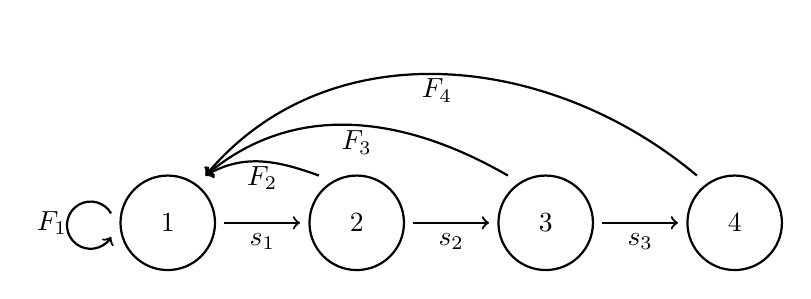
\begin{tikzpicture}[scale=0.6]
	\def\firstcircle{(0,0) circle (1cm)}
	\def\secondcircle{(4,0) circle (1cm)}
	\def\thirdcircle{(8,0) circle (1cm)}
	\def\fourthcircle{(12,0) circle (1cm)}
%	\draw (-4,-4.5) -- (4,-4.5) -- (4,2.75) -- (-4,2.75) -- cycle;
%	\begin{scope}
%	\clip \firstcircle;
%	\draw[fill=gray!30] \secondcircle;
%	\end{scope}
%	\draw[fill=gray!30] \thirdcircle;
	\draw[thick] \firstcircle;
	\draw[thick] \secondcircle;	
	\draw[thick] \thirdcircle;	
	\draw[thick] \fourthcircle;		
	\draw[->, thick](1.2,0) -- (2.8,0);
	\draw[->, thick](5.2,0) -- (6.8,0);
	\draw[->, thick](9.2,0) -- (10.8,0);
	%curve start point, end point, angle at start, angle at end
	\draw[->,thick] (3.2,1.0) to [out=160,in=30](0.8,1.0);
	\draw[->,thick] (7.2,1.0) to [out=150,in=40](0.8,1.0);
	\draw[->,thick] (11.2,1.0) to [out=140,in=50](0.8,1.0);
	\draw[thick] [->] (-1.2,0.2) arc (30:330:0.5); %center of arc, arc (start degree, end degree, radius) 
	\node at (0,0) {$1$};
	\node at (4,0) {$2$};
	\node at (8,0) {$3$};
	\node at (12,0) {$4$};
	\node at (2,-0.4) {$s_1$};
	\node at (6,-0.4) {$s_2$};
	\node at (10,-0.4) {$s_3$};
	\node at (-2.45,0.0) {$F_1$};
	\node at (2,0.95) {$F_2$};
	\node at (4,1.7) {$F_3$};
	\node at (5.7,2.8) {$F_4$};
\end{tikzpicture}
\caption{Life cycle with four age classes.}
\label{F:Life_cycle}
\end{center}
\end{figure}
\end{comment}

To model the sheep population, we need a few variables. Let $n_1^{(0)}$ be the number of sheep in age group 0-1, $n_2^{(0)}$ the number in age group 1-2, $n_3$ the number in age group 2-3 and, in general, $n_k^{(0)}$ the number of sheep in age group $(k-1)$-$k$ at some initial time (time $0$), and let 
\[\vx_0 = \left[ n_1^{(0)} \ n_2^{(0)} \ n_3^{(0)} \ \cdots \ n_{12}^{(0)} \right]^{\tr}.\]
We wish to determine the populations in the different groups after one year. Let 
\[\vx_1 = \left[ n_1^{(1)} \ n_2^{(1)} \ n_3^{(1)}  \ \cdots \ n_{12}^{(1)} \right]^{\tr},\]
where $n_1^{(1)}$ denotes the number of sheep in age group 0-1, $n_2^{(1)}$ the number of sheep in age group 1-2 and, in general, $n_{k}^{(1)}$ the number of tilapia in age group $(k-1)$-$k$ after one year. 

\begin{pactivity} \label{Leslie_1} Table \ref{T:Sheep} shows that, on average, each female in age group 1-2 produces $0.045$ female offspring in a year. Since there are $n_2$ females in age group 1-2, the lamb population increases by $0.045n_2$ in a year. 
	\ba
	\item Continue this analysis to explain why 
	\begin{align*}
	n_1^{(1)} &= 0.045n_2+0.391 n_3+0.472n_4+0.484 n_5+0.546n_6+0.543n_7 \\
		&\qquad+0.502 n_8+0.468 n_9+0.459n_{10}+0.433 n_{11}+0.421 n_{12}.
	\end{align*}
	
	\item Explain why $n_2^{(1)} = 0.845n_1$. 
	
	\item Now explain why 
\begin{equation}
\vx_1 = L\vx_0, \label{eq:Leslie_1}
\end{equation}
where $L$ is the matrix 
 \begin{equation} \label{eq:Leslie_2}
 {\scriptsize \hspace*{-0.25in} \left[\arraycolsep=2.0pt  \begin{array}{cccccccccccc} 
0     	& 0.045 & 0.391 & 0.472 & 0.484 & 0.546 & 0.543 & 0.502 & 0.468 & 0.459 & 0.433 & 0.421 \\
0.845 	& 0 	& 0 	& 0 	& 0 	& 0 	& 0 	& 0 	& 0 	& 0 	& 0 	& 0 \\
0 		& 0.975 & 0		& 0 	& 0 	& 0 	& 0 	& 0 	& 0 	& 0 	& 0 	& 0 \\
0 		& 0 	& 0.965	& 0 	& 0 	& 0 	& 0 	& 0 	& 0 	& 0 	& 0 	& 0 \\
0 		& 0 	& 0		& 0.950	& 0 	& 0 	& 0 	& 0 	& 0 	& 0 	& 0 	& 0 \\
0 		& 0 	& 0		& 0		& 0.926 & 0 	& 0 	& 0 	& 0 	& 0 	& 0 	& 0 \\
0 		& 0 	& 0		& 0		& 0 	& 0.895	& 0 	& 0 	& 0 	& 0 	& 0 	& 0 \\
0 		& 0 	& 0		& 0		& 0 	& 0		& 0.850	& 0 	& 0 	& 0 	& 0 	& 0 \\
0 		& 0 	& 0		& 0		& 0 	& 0		& 0		& 0.786	& 0 	& 0 	& 0 	& 0 \\
0 		& 0 	& 0		& 0		& 0 	& 0		& 0		& 0		& 0.691	& 0 	& 0 	& 0 \\
0 		& 0 	& 0		& 0		& 0 	& 0		& 0		& 0		& 0		& 0.561	& 0 	& 0 \\
0 		& 0 	& 0		& 0		& 0 	& 0		& 0		& 0		& 0		& 0		& 0.370	& 0 \\
\end{array} \right]}.
\end{equation}

	\ea
\end{pactivity}

Notice that our matrix $L$ has the form 
\[\left[ \begin{array}{cccccc} F_1&F_2&F_3&\cdots&F_{n-1}&F_n \\ s_1&0&0&\cdots&0&0 \\ 0&s_2&0&\cdots&0&0 \\  0&0&s_3&\cdots&0&0 \\ &&&\ddots&& \\ 0&0&0&\cdots&s_{n-1}&0 \end{array} \right].\]
Such a matrix is called a \emph{Leslie matrix}\index{Leslie matrix}\index{Leslie matrix}. 

Leslie matrices have certain useful properties, and one eigenvalue of a Leslie matrix can tell us a lot about the long-term behavior of the situation being modeled. You can take these properties as fact unless otherwise directed.
\begin{enumerate}
\item A Leslie matrix $L$ has a unique positive eigenvalue $\lambda_1$ with a corresponding eigenvector $\vv_1$ whose entries are all positive.

\item If $\lambda_i$ ($i > 1$) is any other eigenvalue (real or complex) of $L$, then $|\lambda_i| \leq \lambda_1$. If $\lambda_1$ is the largest magnitude eigenvalue of a matrix $L$, we call $\lambda_1$ a \emph{dominant eigenvalue} of $L$.

\item If any two successive entries in the first row of $L$ are both positive, then $|\lambda_i| < \lambda_1$ for every $i > 1$. In this case we say that $\lambda_1$ is a \emph{strictly dominant eigenvalue} of $L$. In a Leslie model, this happens when the females in two successive age classes are fertile, which is almost always the case.

\item If $\lambda_1$ is a strictly dominant eigenvalue, then $\vx_k$ is approximately a scalar multiple of $\vv_1$ for large values of $k$, regardless of the initial state $\vx_0$. In other words, large state vectors are close to eigenvectors for $\lambda_1$.
\end{enumerate}

We can use these properties to determine the long-term behavior of the sheep herd.

\begin{pactivity} \label{act:Leslie_2} Assume that $L$ is defined by (\ref{eq:Leslie_2}), and let 
\[\vx_m = \left[ n_1^{(m)} \ n_2^{(m)} \ n_3^{(m)} \ \cdots \ n_{12}^{(m)} \right]^{\tr},\]
 where $n_1^{(m)}$ denotes the number of sheep in age group 0-1, $n_2^{(m)}$ the number of sheep in age group 1-2 and, in general, $n_k^{(m)}$ the number of sheep in age group $(k-1)$-$k$ after $k$ years. 
 	\ba
	 \item Assume that $\vx_0 = \left[100 \ 100 \ 100 \ \cdots \ 100  \right]^{\tr}$. Use appropriate technology to calculate $\vx_{22}$, $\vx_{23}$, $\vx_{24}$, and $\vx_{25}$. Round to the nearest whole number. What do you notice about the sheep population?  You may use the GeoGebra applet at \url{https://www.geogebra.org/m/yqss88xq}. 

	\item  We can use the third and fourth properties of Leslie matrices to better understand the long-term behavior of the sheep population. Since successive entries in the first row of the Leslie matrix in (\ref{eq:Leslie_2}) are positive, our Leslie matrix has a strictly dominant eigenvalue $\lambda_1$. Given the dimensions of our Leslie matrix, finding this dominant eigenvalue through algebraic means is not feasible. Use the power method to approximate the dominant eigenvalue $\lambda_1$ of the Leslie matrix in (\ref{eq:Leslie_2}) to five decimal places. Explain your process. Then explain how this dominant eigenvalue tells us that, unchecked, the sheep population grows at a rate that is roughly exponential. What is the growth rate of this exponential growth?  You may use the GeoGebra applet at \url{https://www.geogebra.org/m/yqss88xq}. 

	\ea

\end{pactivity}


Project Activity \ref{act:Leslie_2} indicates that, unchecked, the sheep population will grow without bound, roughly exponentially with ratio equal to the dominant eigenvalue of our Leslie matrix $L$. Of course, a sheep farmer cannot provide the physical environment or the resources to support an unlimited population of sheep. In addition, most sheep farmers cannot support themselves only by shearing sheep for the wool. Consequently, some harvesting of the sheep population each year for meat and skin is necessary. A sustainable harvesting policy allows for the regular harvesting of some sheep while maintaining the population at a stable level. It is necessary for the farmer to find an optimal harvesting rate to attain this stable population and the following activity leads us through an analysis of how such a harvesting rate can be determined.

\begin{pactivity} \label{act:Leslie_harvest} The Leslie model can be modified to consider harvesting. It is possible to harvest different age groups at different rates, and to harvest only some age groups and not others. In the case of sheep, it might make sense to only harvest from the youngest population since lamb is more desirable than mutton and the lamb population grows the fastest. Assume that this is our harvesting strategy and that we harvest our sheep from only the youngest age group at the start of each year. Let $h$ be the fraction of sheep we harvest from the youngest age group each year after considering growth.
\ba
\item If we begin with an initial population $\vx_0$, then the state vector after births and expected deaths is $L\vx_0$. Now we harvest. Explain why if we harvest a fraction $h$ from the youngest age group after considering growth, then the state vector after 1 year will be
\begin{equation*}
\vx_1 = L\vx_0 - HL\vx_0,
\end{equation*}
where
\[H =  \left[
\begin{array}{c c c c c c c c c c c c}
h    	& 0 	& 0 	& 0 	& 0 	& 0 	& 0 	& 0	 	& 0 	& 0 	& 0 	& 0 \\
0 		& 0 	& 0 	& 0 	& 0 	& 0 	& 0 	& 0 	& 0 	& 0 	& 0 	& 0 \\
0 		& 0 	& 0		& 0 	& 0 	& 0 	& 0 	& 0 	& 0 	& 0 	& 0 	& 0 \\
0 		& 0 	& 0		& 0 	& 0 	& 0 	& 0 	& 0 	& 0 	& 0 	& 0 	& 0 \\
0 		& 0 	& 0		& 0		& 0 	& 0 	& 0 	& 0 	& 0 	& 0 	& 0 	& 0 \\
0 		& 0 	& 0		& 0		& 0 	& 0 	& 0 	& 0 	& 0 	& 0 	& 0 	& 0 \\
0 		& 0 	& 0		& 0		& 0 	& 0		& 0 	& 0 	& 0 	& 0 	& 0 	& 0 \\
0 		& 0 	& 0		& 0		& 0 	& 0		& 0		& 0 	& 0 	& 0 	& 0 	& 0 \\
0 		& 0 	& 0		& 0		& 0 	& 0		& 0		& 0		& 0 	& 0 	& 0 	& 0 \\
0 		& 0 	& 0		& 0		& 0 	& 0		& 0		& 0		& 0		& 0 	& 0 	& 0 \\
0 		& 0 	& 0		& 0		& 0 	& 0		& 0		& 0		& 0		& 0		& 0 	& 0 \\
0 		& 0 	& 0		& 0		& 0 	& 0		& 0		& 0		& 0		& 0		& 0		& 0 \\
\end{array} \right].\]


\item Our goal is to find a harvesting rate that will lead to a steady state in which the sheep population remains the same each year. In other words, we want to find a value of $h$, if one exists, that satisfies
\begin{equation}
\vx = L\vx - HL\vx. \label{eq:Harvest}
\end{equation}
Show that (\ref{eq:Harvest}) is equivalent to the matrix equation
\begin{equation}
\vx = (I_{12}-H)L\vx. \label{eq:Harvest2}
\end{equation}

\item Use appropriate technology to experiment numerically with different values of $h$ to find the value you think gives the best uniform harvest rate. Explain your reasoning. You may use the GeoGebra applet at \url{https://www.geogebra.org/m/yqss88xq}. 


\item Now we will use some algebra to find an equation that explicitly gives us the harvest rate in the general setting. This will take a bit of work, but none of it is too difficult. To simplify our work but yet illustrate the overall idea, let us consider the general $4 \times 4$ case with arbitrary Leslie matrix
\begin{equation*} 
L = \left[ \begin{array}{cccc}
F_1 & F_2 	& F_3 	& F_4 \\
s_1 & 0 	& 0 	& 0  \\
0 	& s_2 	& 0 	& 0 \\
0 	& 0 	& s_3	& 0  \\
\end{array} \right].
\end{equation*}
Recall that we want to find a value of $h$ that satisfies (\ref{eq:Harvest2}) with $H = \left[ \begin{array}{cccc}
h   & 0 	& 0 	& 0 \\
0   & 0 	& 0 	& 0  \\
0 	& 0 	& 0 	& 0 \\
0 	& 0 	& 0	    & 0  \\
\end{array} \right].$
Let $\vx = [x_1 \  x_2 \ x_3 \ x_4]^{\tr}$.
        \begin{enumerate}[i.]
        \item Calculate the matrix product $(I_{4}-H)L$. Explain why this product is again a Leslie matrix and why $(I_{4}-H)L$ will have a dominant eigenvalue of 1.


        \item Now calculate $(I_{4}-H)L\vx$ and set it equal to $\vx$. Write down the resulting system of 4 equations that must be satisfied. Be sure that your first equation is
\begin{equation}
x_1 = (1-h)F_1x_1 + (1-h)F_2x_2 + (1-h)F_3x_3 + (1-h)F_4x_4. \label{eq:harvestval1}
\end{equation}

        \item Equation (\ref{eq:harvestval1}) as written depends on the entries of the vector $\vx$, but we should be able to arrive at a result that is independent of $\vx$. To see how we do this, we assume the population of the youngest group is never 0, so we can divide both sides of (\ref{eq:harvestval1}) by $x_1$ to obtain
\begin{equation} 
1 = (1-h)F_1 + (1-h)F_2 \frac{x_2}{x_1} + (1-h)F_3 \frac{x_3}{x_1} + (1-h)F_4 \frac{x_4}{x_1}. \label{eq:harvestval2}
\end{equation}
Now we need to write the fractions $\frac{x_2}{x_1}$,   $\frac{x_3}{x_1}$,  and $\frac{x_4}{x_1}$ so that they do not involve the $x_i$. Use the remaining equations in your system to show that
\begin{align*}
\frac{x_2}{x_1} &= s_1 \\
\frac{x_3}{x_1} &= s_1s_2 \\
\frac{x_4}{x_1} &= s_1s_2s_3. \\
\end{align*}


\item Now conclude that the harvesting value $h$ must satisfy the equation
\begin{equation}
1 = (1-h) [F_1 + F_2 s_1 + F_3 s_1s_2 + F_4 s_1s_2s_3]. \label{eq:harvestval3}
\end{equation}
The value $R = F_1 + F_2 s_1 + F_3 s_1s_2 + F_4 s_1s_2s_3$ is called the \emph{net reproduction rate of the population} and turns out to be the average number of daughters born to a female in her expected lifetime.


        \end{enumerate}

\item Extend (\ref{eq:harvestval3}) to the 12 age group case of the sheep herd. Calculate the value of $R$ for this sheep herd and then find the value of $h$. Compare this $h$ to the value you obtained through experimentation earlier. Find the fraction of the lambs that should be harvested each year and explain what the stable population state vector $\vx$ tells us about the sheep population for this harvesting policy.


\ea
\end{pactivity}



 %20
\achapter{21}{Complex Eigenvalues} \label{sec:complex_eigenvalues}

\vspace*{-17 pt}
\framebox{
\parbox{\dimexpr\linewidth-3\fboxsep-3\fboxrule}
{\begin{fqs}
\item What properties do complex eigenvalues of a real matrix satisfy?
\item What properties do complex eigenvectors of a real matrix satisfy?
\item What is a rotation-scaling matrix?
\item How do we find a rotation-scaling matrix within a matrix with complex eigenvalues?
\end{fqs}}}% \hspace*{3 pt}}

\vspace*{13 pt}

\csection{Application: The Gershgorin Disk Theorem}

We have now seen different methods for calculating/approximating eigenvalues of a matrix. The algebraic method using the characteristic polynomial can provide exact values, but only in cases where the size of the matrix is small. Methods like the power method allow us to approximate eigenvalues in many, but not all, cases. These approximation techniques can be made more efficient if we have some idea of where the eigenvalues are. The Gershgorin Disc Theorem is a useful tool that can quickly provide bounds on the location of eigenvalues using elementary calculations. For example, using the Gershsgorin Disk Theorem we can quickly tell that the real parts of the eigenvalues of the matrix 
\[\left[ \begin{array}{ccr} 3&1&-1 \\ 0&-1+i&i \\ 2&1&-2i \end{array} \right]\]
lie between $-4$ and 5 and the imaginary parts lie between $-5$ and 2. Even more, we can say that the eigenvalues lie in the disks (called \emph{Gershgorin disks}) shown in Figure \ref{F:Gershgorin_1}.
\begin{figure}[ht]
\begin{center}
\resizebox{!}{2.5in}{\includegraphics{Gershgorin_1.eps}}
\end{center}
\caption{Gershgorin disks.}
\label{F:Gershgorin_1}
\end{figure}
We will learn more details about the Gershgorin Disk Theorem at the end of this section. 

\csection{Introduction}

So far we have worked with real matrices whose eigenvalues are all real. However, the characteristic polynomial of a matrix with real entries can have complex roots. In this section we investigate the properties of these complex roots and their corresponding eigenvectors, how these complex eigenvectors are found, and the geometric interpretation of the transformations defined by matrices with complex eigenvalues. Although we can consider matrices that have complex numbers as entries, we will restrict ourselves to matrices with real entries. 

\begin{pa} \label{pa:4_e} Let $A = \left[ \begin{array}{rc} 2&4 \\ -2&2 \end{array} \right]$.
	\be
	\item Find the characteristic polynomial of $A$.

	\item Find the eigenvalues of $A$. You should get two complex numbers. How are these complex numbers related?

	\item Find an eigenvector corresponding to each eigenvalue of $A$. You should obtain vectors with complex entries.

	\ee
\end{pa}

\csection{Complex Eigenvalues}

As you noticed in Preview Activity \ref{pa:4_e}, the complex roots of the characteristic equation of a real matrix $A$ come in complex conjugate pairs. This should come as no surprise since we know through our use of the quadratic formula that complex roots of (real) quadratic polynomials come in complex conjugate pairs. More generally, if $p(x)=a_0+a_1x+a_2x^2 + \cdots + a_nx^n$ is a polynomial with real coefficients and $z$ is a root of this polynomial, meaning $p(z)=0$, then 
\[ 0=\overline{p(z)} = \overline{a_0+a_1z+a_2z^2 + \cdots + a_nz^n} = a_0 + a_1 \overline{z} + a_2 \overline{z}^2 + \cdots + a_n \overline{z}^n = p(\overline{z})\, .\]
Therefore, $\overline{z}$ is also a root of $p(x)$.

\begin{activity} \label{act:4e_1} Let $A=\left[ \begin{array}{cr} 0&-1 \\ 1&0 \end{array} \right]$. 

	\ba
	\item The matrix transformation $T:\R^2 \to \R^2$ defined by $T(\vx)=A\vx$ is a rotation transformation. What is the angle of rotation?
	
	
	
	\item Find the eigenvalues of $A$. For each eigenvalue, find an eigenvector.

	
		
	\ea
\end{activity}



In Preview Activity \ref{pa:4_e} and in Activity \ref{act:4e_1}, you found that if $\vv$ is an eigenvector of $A$ corresponding to $\lambda$, then $\overline{\vv}$ obtained by taking the complex conjugate of each entry in $\vv$ is an eigenvector of $A$ corresponding to $\overline{\lambda}$. Specifically, if $\vv=\vu+i\vw$ where both $\vu$ and $\vw$ are real vectors is an eigenvector of $A$, then so is $\overline{\vv} = \vu-i\vw$. We can justify this property using matrix algebra as follows:
\[ A\overline{\vv} = \overline{A}\overline{\vv} = \overline{A\vv} = \overline{\lambda \vv} = \overline{\lambda} \overline{\vv} \, .\]
In the first equality, we used the fact that $A$ is a real matrix, so $\overline{A}=A$. In all the other equalities, we used the properties of the conjugation operation in complex numbers.

\csection{Rotation and Scaling Matrices}

Recall that a rotation matrix is of the form 
\[ R_\theta= \left[ \begin{array}{cr} \cos(\theta)&-\sin(\theta) \\ \sin(\theta)&\cos(\theta) \end{array} \right]\]
where the rotation is counterclockwise about the origin by an angle of $\theta$ radians. In Activity \ref{act:4e_1}, we considered the rotation matrix with angle $\pi/2$ in counterclockwise direction. We will soon see that rotation matrices play an important role in the geometry of a matrix transformation for a matrix that has complex eigenvalues. In this activity, we will restrict ourselves to the $2 \times 2$ case, but similar arguments can be made in higher dimensions.



\begin{activity} \label{act:4e_2} Let $A=\left[ \begin{array}{rc} 1&1 \\ -1&1 \end{array} \right]$. 

	\ba
	\item Explain why $A$ is not a rotation matrix.
	
	
	
	\item Although $A$ is not a rotation matrix, there is a rotation matrix $B$ inside $A$. To find the matrix $B$, factor out $\sqrt{2}$ from all entries of $A$. In other words, write $A$ as a product of two matrices in the form
\[ A = \left[ \begin{array}{cc} \sqrt{2} &0 \\ 0&\sqrt{2} \end{array} \right] B \;. \]
		
	
		
	\item The $B$ matrix is a rotation matrix with an appropriate $\theta$. Find this $\theta$.
	
	
	
	\item If we think about the product of two matrices as applying one transformation after another, describe the effect of the matrix transformation defined by $A$ geometrically. 

	 		
			
	\ea
\end{activity}



More generally, if we have a matrix $A$ of the form $A=\left[ \begin{array}{cr} a&-b \\ b&a \end{array} \right]$, then 
\[ A = \left[ \begin{array}{cc} \sqrt{a^2+b^2} &0 \\ 0&\sqrt{a^2+b^2} \end{array} \right] \left[ \begin{array}{cc} \frac{a}{\sqrt{a^2+b^2}}&\frac{-b}{\sqrt{a^2+b^2}} \\ \frac{b}{\sqrt{a^2+b^2}}&\frac{a}{\sqrt{a^2+b^2}}\end{array} \right] \, .\]
The first matrix in the decomposition is a scaling matrix with a scaling factor of $s=\sqrt{a^2+b^2}$. So if $s>1$, the transformation stretches vectors, and if $s<1$, the transformation shrinks vectors. The second matrix in the decomposition is a rotation matrix with angle $\theta$ such that $\cos(\theta)=\frac{a}{\sqrt{a^2+b^2}}$ and $\sin(\theta)=\frac{b}{\sqrt{a^2+b^2}}$. This angle is also the angle between the positive $x$-axis and the vector $\vv=\left[ \begin{array}{c} a\\ b\end{array} \right]$. We will refer to the matrices of the form $\left[ \begin{array}{cr} a&-b \\ b&a \end{array} \right]$ as \emph{rotation-scaling matrices}\index{rotation-scaling matrices}. 

\csection{Matrices with Complex Eigenvalues}

Now we will investigate how a general $2\times 2$ matrix with complex eigenvalues can be seen to be similar (both in a linear algebra and a colloquial meaning) to a rotation-scaling matrix.



\begin{activity} \label{act:4e_3} Let $B=\left[ \begin{array}{cr} 1&-5\\2&3 \end{array} \right]$. The eigenvalues of $B$ are $2\pm 3i$.  An eigenvector for the eigenvalue $2-3i$ is $\vv=\left[ \begin{array}{c} -5 \\ 1-3i\end{array} \right]$. We will use this eigenvector to show that $B$ is similar to a rotation-scaling matrix.

	\ba
	\item Any complex vector $\vv$ can be written as $\vv=\vu+i\vw$ where both $\vu$ and $\vw$ are real vectors. What are these real vectors $\vu$ and $\vw$ for the eigenvector $\vv$ above?
	
	
	
	\item Let $P=[ \vu \ \vw ]$ be the matrix whose first column is the real part of $\vv$ and whose second column is the imaginary part of $\vv$ (without the $i$). Find $R=P^{-1}BP$.
		
	
		
	\item Express $R$ as a product of a rotation and a scaling matrix. What is the factor of scaling? What is the rotation angle?
	
	
				
	\ea
\end{activity}



In Activity \ref{act:4e_3}, we saw that the matrix $B$ with complex eigenvalues $2\pm 3i$ is similar to a rotation-scaling matrix. Specifically $R=P^{-1}BP$, where the columns of $P$ are the real and imaginary parts of an eigenvector of $B$, is the rotation-scaling matrix with a factor of scaling by $\sqrt{2^2+3^2}$ and a rotation by angle $\theta=\arccos(\frac{2}{\sqrt{2^2+3^2}})$. 



Does a similar decomposition result hold for a general $2\times 2$ matrix with complex eigenvalues? We investigate this question in the next activity.



\begin{activity} \label{act:4e_4} Let $A$ be a $2\times 2$ matrix with complex eigenvalue $\lambda=a-bi$, $b\neq 0$, and corresponding complex eigenvector $\vv=\vu+i\vw$.

	\ba
	\item Explain why $A\vv = A\vu+iA\vw$.
	
	
	\item Explain why $\lambda\vv = (a\vu+b\vw)+i (a\vw-b\vu)$.
		
	
		
	\item Use the previous two results to explain why 
	\begin{itemize}
	\item $A\vu=a\vu+b\vw$ and 
	\item $A\vw = a\vw - b\vu$.
	\end{itemize}
	
	
	
	\item Let $P=[ \vu \ \vw ]$. We will now show that $AP=PR$ where $R=\left[ \begin{array}{cr} a&-b \\ b&a \end{array} \right]$.
	
	\begin{enumerate}[i.]
	\item Without any calculation, explain why
\[AP = [ A\vu \  A\vw ].\]



	\item Recall that if $M$ is an $m \times n$ matrix and $\vx$ is an $n \times 1$ vector, then the matrix product $M\vx$ is a linear combination of the columns of $M$ with weights the corresponding entries of the vector $\vx$. Use this idea to show that
\[PR = [ a\vu + b\vw \  -b\vu + a\vw ].\]



	\item Now explain why $AP = PR$.
	
	
	
	\item Assume for the moment that $P$ is an invertible matrix. Show that $A = PRP^{-1}$.
	
	
	
	\end{enumerate}
				
	\ea
\end{activity}



Your work in Activity \ref{act:4e_4} shows that any $2\times 2$ matrix is similar to a rotation-scaling matrix with a factor of scaling by $\sqrt{a^2+b^2}$ and a rotation by angle $\theta=\arccos(\frac{a}{\sqrt{a^2+b^2}})$ if $b\geq 0$, and $\theta=-\arccos(\frac{a}{\sqrt{a^2+b^2}})$ if $b<0$. Geometrically, this means that every $2 \times 2$ real matrix with complex eigenvalues is just a scaled rotation ($R$) with respect to the basis $\B$ formed by $\vu$ and $\vw$ from the complex eigenvector $\vv$. Multiplying by $P^{-1}$ and $P$ simply provides the change of basis from the standard basis to the basis $\B$, as we will see in detail when we learn about linear transformations.



\begin{theorem} Let $A$ be a real $2\times 2$ matrix with complex eigenvalue $a-bi$ and corresponding eigenvector $\vv=\vu+i\vw$. Then 
\[ A=PRP^{-1} \; , \text{ where } P=[ \vu \ \vw ] \; \text{ and } R= \left[ \begin{array}{cr} a&-b \\ b&a \end{array} \right] \, .\]
\end{theorem}



The one fact that we have not yet addressed is why the matrix $P = [ \vu \ \vw ]$ is invertible. We do that now to complete the argument.

Let $A$ be a real $2 \times 2$ matrix with $A \vv = \lambda \vv$, where $\lambda = a-bi$, $b \neq 0$ and $\vv=\vu+i\vw$ (where $\vu$ and $\vv$ are in $\R^2$) with $\vw \neq \vzero$. From Activity \ref{act:4e_4} we know that 
\[A\vu = a\vu + b\vw \ \text{ and } \ A\vw = a\vw - b \vu.\]

To show that $\vu$ and $\vw$ are linearly independent, we need to show that no nontrivial linear combination of $\vu$ and $\vw$ can be the zero vector. Suppose
\[x_1\vu + x_2\vw = \vzero\]
for some scalars $x_1$ and $x_2$. We will show that $x_1 = x_2 = 0$. Assume to the contrary that one of $x_1, x_2$ is not zero. First, assume $x_1 \neq 0$. Then $\vu = -\frac{x_2}{x_1} \vw$. Let $c = -\frac{x_2}{x_1}$. From this we have
\begin{align*}
A \vu &= A(c\vw) \\
A \vu &= cA \vw \\
a\vu + b\vw &= c(a \vw - b \vu) \\
(a+cb)\vu &= (ca-b)\vw \\
(a+cb)(c\vw) &= (ca-b)\vw.
\end{align*}
Since $\vw \neq \vzero$ we must have $(a+cb)c = ca-b$. A little algebra shows that $(c^2+1)b = 0$. Since $b \neq 0$, we conclude that $c^2+1=0$, which is impossible for a real constant $c$. Therefore, we cannot have $x_1 \neq 0$. A similar argument (left to the reader) shows that $x_2 = 0$. Thus we can conclude that $\vu$ and $\vw$ are linearly independent.

\csection{Examples}

\ExampleIntro

\begin{example} Let $A = \left[ \begin{array}{rcr} 0&1&0 \\ -1&0&-1 \\ 1&1&1 \end{array} \right]$.
\ba
\item Without doing any computations, explain why not all of the eigenvalues of $A$ can be complex.

\item Find all of the eigenvalues of $A$.

\ea

\ExampleSolution
\ba
\item Since complex eigenvalues occur in conjugate pairs, the complex eigenvalues with nonzero imaginary parts occur in pairs. Since $A$ can have at most 3 different eigenvalues, at most two of them can have nonzero imaginary parts. So at least one eigenvalue of $A$ is real. 

\item For this matrix $A$ we have $A - \lambda I_3 = \left[ \begin{array}{rrc} -\lambda&1&0 \\ -1&-\lambda&-1 \\ 1&1&-\lambda+1 \end{array} \right]$. Using a cofactor expansion along the first row gives us 
\begin{align*}
\det(A - \lambda I_3) &= (-\lambda)\left((-\lambda)(1-\lambda)+1\right) - \left((-1)(1-\lambda)+1\right) \\
	&= -\lambda^3 + \lambda^2 - \lambda +1 - \lambda -1 \\
	&= \lambda^3 + \lambda^2 - 2\lambda \\
	&= -\lambda(\lambda^2 -\lambda + 2).
\end{align*}
The roots of the characteristic polynomial are $\lambda = 0$ and 
\[\lambda = \frac{1 \pm \sqrt{1-4(2)}}{2} = \frac{1}{2}(1 \pm \sqrt{7}i).\]


\ea


\end{example}

\begin{example} Let $A = \left[ \begin{array}{rc} 1&2\\-1&3 \end{array} \right]$.  Find a rotation scaling matrix $R$ that is similar to $A$. Identify the rotation and scaling factor.


\ExampleSolution
The eigenvalues of $A$ are the roots of the characteristic polynomial
\begin{align*}
p(\lambda) &= \det(A - \lambda I_2) \\
	&= \det\left(\left[ \begin{array}{rc} 1-\lambda&2\\-1&3-\lambda \end{array} \right]\right) \\
	&= (1-\lambda)(3-\lambda) + 2 \\
	&= \lambda^2 -4\lambda + 5.
\end{align*}
The quadratic formula shows that the roots of $p(\lambda)$ are 
\[\frac{4 \pm \sqrt{-4}}{2} = 2 \pm i.\]
To find an eigenvector for $A$ with eigenvalue $2-i$, we row reduce 
\[A - (2-i) I_3 =   \left[ \begin{array}{cc} -1+i&2\\-1&1+i \end{array} \right]\]
to 
\[\left[ \begin{array}{cc} 1&-i-1\\0&0 \end{array} \right].\]
An eigenvector for $A$ with eigenvalue $2-i$ is then 
\[[ 1+i \  \ 1]^{\tr} = [1 \ 1]^{\tr} + i[1 \ 0]^{\tr}.\]
Letting $P = \left[  \begin{array}{cc} 1&1\\1&0 \end{array} \right]$, we have 
\[R = P^{-1}AP = \left[ \begin{array}{cr} 2&-1\\1&2 \end{array} \right].\]
The scaling is determined by the determinant of $R$ which is $5$, and the angle $\theta$ of rotation satisfies $\sin(\theta) = \frac{1}{5}$. This makes  $\theta \approx 0.2014$ radians or approximately $11.5370^{\circ}$ counterclockwise. 


\end{example}



\csection{Summary}

\begin{itemize}
\item For a real matrix, complex eigenvalues appear in conjugate pairs. Specifically, if $\lambda=a+ib$ is an eigenvalue of a real matrix $A$, then $\overline{\lambda}=a-ib$ is also an eigenvalue of $A$.
\item For a real matrix, if a $\vv$ is an eigenvector corresponding to $\lambda$, then the vector $\overline{\vv}$ obtained by taking the complex conjugate of each entry in $\vv$ is an eigenvector corresponding to $\overline{\lambda}$.
\item The rotation-scaling matrix $A=\left[ \begin{array}{cr} a&-b \\ b&a \end{array} \right]$ can be written as 
\[ \left[ \begin{array}{cc} \sqrt{a^2+b^2} &0 \\ 0&\sqrt{a^2+b^2} \end{array} \right] \left[ \begin{array}{cc} \frac{a}{\sqrt{a^2+b^2}}&\frac{-b}{\sqrt{a^2+b^2}} \\ \frac{b}{\sqrt{a^2+b^2}}&\frac{a}{\sqrt{a^2+b^2}}\end{array} \right] \, .\]
This decomposition geometrically means that the transformation corresponding to $A$ can be viewed as a rotation by angle $\theta=\arccos\left(\frac{a}{\sqrt{a^2+b^2}}\right)$ if $b\geq 0$, or $\theta=-\arccos\left(\frac{a}{\sqrt{a^2+b^2}}\right)$ if $b<0$, followed by a scaling by factor $\sqrt{a^2+b^2}$. 
\item If $A$ is a real $2\times 2$ matrix with complex eigenvalue $a-bi$ and corresponding eigenvector $\vv=\vu+i\vw$, then $A$ is similar to the rotation-scaling matrix $R=\left[ \begin{array}{cr} a&-b \\ b&a \end{array} \right]$. More specifically,
\[ A=PRP^{-1} \; , \text{ where } P=[ \vu \ \vw ]\, .\]
\end{itemize}


\csection{Exercises}
\be
\item Find eigenvalues and eigenvectors of each of the following matrices.
\ba \item $\left[ \begin{array}{rc} 2&4 \\ -2&2 \end{array} \right]$
\item $\left[ \begin{array}{rc} 3&2 \\ -1&1 \end{array} \right]$
\item $\left[ \begin{array}{cr} 1&-2 \\ 4&-3 \end{array} \right]$
\ea

\item Find a rotation-scaling matrix where the rotation angle is $\theta=3\pi/4$ and scaling factor is less than 1.

\item Determine which rotation-scaling matrices have determinant equal to 1. Be as specific as possible.

\item Determine the rotation-scaling matrix inside the matrix $\left[ \begin{array}{rc} 2&4 \\ -2&2 \end{array} \right]$.

\item Find a real $2\times 2$ matrix with eigenvalue $1+2i$.

\item Find a real $2\times 2$ matrix which is not a rotation-scaling matrix with eigenvalue $-1+2i$.

\item We have seen how to find the characteristic polynomial of an $n \times n$ matrix. In this exercise we consider the reverse question. That is, given a polynomial $p(\lambda)$ of degree $n$, can we find an $n \times n$ matrix whose characteristic polynomial is $p(\lambda)$? 
\ba
\item Find the characteristic polynomial of the $2 \times 2$ matrix $C = \left[ \begin{array}{cc} 0&-a_0\\1&-a_1 \end{array} \right]$. Use this result to find a real valued matrix whose eigenvalues are $1+i$ and $1-i$. 

\item Repeat part (a) by showing that $p(\lambda) = -\left(\lambda^3+a_2\lambda^2+a_1\lambda+a_0\right)$ is the characteristic polynomial of the $3 \times 3$ matrix $C = \left[ \begin{array}{ccc} 0&0&-a_0\\1&0&-a_1\\0&1&-a_2 \end{array} \right]$.  

\item We can generalize this argument. Prove, using mathematical induction, that the polynomial
\[p(\lambda) =(-1)^n\left( \lambda^n + a_{n-1}\lambda^{n-1} + a_{n-2}\lambda^{n-2} + \cdots + a_1 \lambda + a_0\right)\]
is the characteristic polynomial of the matrix 
\[C = \left[ \begin{array}{cccccc} 0&0&0&\cdots&0&-a_{0}\\
1&0&0&\cdots&0&-a_{1} \\
0&1&0&\cdots&0&-a_2 \\
\vdots & \vdots &\vdots& \ddots & \vdots   & \vdots   \\
0 & 0 & 0& \cdots &  1 & -a_{n-1} 
\end{array} \right].\]
The matrix $C$ is called the \emph{companion matrix}\index{companion matrix} for $p(\lambda)$.

\ea


\item Label each of the following statements as True or False. Provide justification for your response.
\ba
\item \textbf{True/False} If $3-4i$ is an eigenvalue of a real matrix, then so is $3+4i$.

\item \textbf{True/False} If $2+3i$ is an eigenvalue of a $3\times 3$ real matrix $A$, then $A$ has three distinct eigenvalues.

\item \textbf{True/False} Every $2\times 2$ real matrix with complex eigenvalues is a rotation-scaling matrix.

\item \textbf{True/False} Every square matrix with real entries has real number eigenvalues. 

\item \textbf{True/False} If $A$ is a $2\times 2$ matrix with complex eigenvalues similar to a rotation-scaling matrix $R$, the eigenvalues of $A$ and $R$ are the same.

\item \textbf{True/False} If $A$ is a real matrix with complex eigenvalues, all eigenvectors of $A$ must be non-real.


\ea

\ee

\csection{Project: Understanding the Gershgorin Disk Theorem}

To understand the Gershgorin Disk Theorem, we need to recall how to visualize a complex number in the plane. Recall that a complex number $z$ is a number of the form $z = a+bi$ where $a$ and $b$ are real numbers and $i^2 = -1$. The number $a$ is the real part of $z$, denoted as $\text{Re}(z)$, and $b$ is the imaginary part of $z$, denoted $\text{Im}(z)$. The set of all complex numbers is denoted $\C$. We define addition and multiplication on $\C$ as follows. For $a+bi, c+di \in \C$, 
\[(a+bi) + (c+di) = (a+c) + (b+d)i \ \ \ \ \ \text{and} \ \ \ \ \ (a+bi)(c+di) = (ac-bd) + (ad+bc)i.\]
Note that the product is what we would expect if we ``expanded" the product in the normal way and used the fact that $i^2=-1$. The set of complex numbers forms a field -- that is, $\C$ satisfies all of the same properties as $\R$ as stated in Theorem \ref{thm:1_d_reals}. 

We can visualize the complex number $a+bi$ in the plane as the point $(a,b)$. Here we are viewing the horizontal axis as the real axis and the vertical axis as the imaginary axis. The length (or magnitude) of the complex number $z = a+bi$, which we denote as $|z|$, is the distance from the origin to $z$. So by the Pythagorean Theorem we have $|a+bi| = \sqrt{a^2+b^2}$. Note that the magnitude of $z = a+bi$ can be written as a complex product 
\[|z| = \sqrt{(a+bi)(a-bi)}.\]
The complex number $a-bi$ is called the \emph{complex conjugate} of $z=a+bi$ and is denoted as $\overline{z}$. A few important properties of real numbers and their conjugates are the following. Let $z = a+bi$ and $w = c+di$ be complex numbers. Then

\begin{itemize}
\item $\overline{z+w} = \overline{(a+c) + (b+d)i} = (a+c)-(b+d)i = (a-bi) + (c-di) = \overline{z} + \overline{w}$,
\item $\overline{zw} = \overline{(ac-bd) + (ad+bc)i} = (ac-bd)-(ad+bc)i = (a-bi)(c-di) = \overline{z} \overline{w}$,
\item $\overline{\overline{z}} = z$,
%\item $\Re(z\overline{w}) = \Re((ac+bd) + (bc-ad)i) = ac+bd$,
%\item $\Im(z\overline{w}) = bc-ad$,
\item $|z| = \sqrt{a^2+b^2} \geq \sqrt{a^2} = |a| = |\text{Re}(z)|$,
\item $|z| = \sqrt{a^2+b^2} \geq \sqrt{b^2} = |b| = |\text{Im}(z)|$,
\item $\left| \overline{z} \right| = |z|$,
\item $|z| = 0$ if and only if $z = 0$,
\item If $p(x)$ is a polynomial with real coefficients and the complex number $z$ satisfies $p(z) = 0$, then $p\left(\overline{z}\right) = 0$ as well. 
\end{itemize}

Using these facts we can show that the triangle inequality is true for complex numbers. That is, 
\[|z+w| \leq |z| + |w|.\]
To see why, notice that 
\begin{align*}
|z+w|^2 &= (z+w)(\overline{z+w}) \\
	&= (z+w)(\overline{z} + \overline{w}) \\
	&= z\overline{z} + z\overline{w} + w \overline{z} + w \overline{w} \\
	&= z\overline{z} + z\overline{w} + \overline{zw\overline{w}} + w \overline{w} \\
%	&= |z|^2 + [(ac+bd) + (bc-ad)i] + [(ca+db) + (da-cb)i] + |w|^2 \\
	&= |z|^2 + 2\text{Re}(z\overline{w}) + |w|^2 \\
	&\leq |z|^2 + 2|zw| + |w|^2 \\
	&= |z|^2 + 2|z| |w| + |w|^2 \\
	&= (|z|+|w|)^2.
\end{align*}
Since $|z+w|$, $|z|$, and $|w|$ are all non-negative, taking square roots of both sides gives us $|z+w| \leq |z| + |w|$ as desired. We can extend this triangle inequality to any number of complex numbers. That is, if $z_1$, $z_2$, $\ldots$, $z_k$ are complex numbers, then 
\begin{equation} \label{eq:general_triangle_inequaltity}
|z_1+z_2+ \cdots + z_k| \leq |z_1| + |z_2| + \cdots + |z_k|.
\end{equation}
We can prove Equation (\ref{eq:general_triangle_inequaltity}) by mathematical induction. We have already done the $k=2$ case and so we assume that Equation (\ref{eq:general_triangle_inequaltity}) is true for any sum of $k$ complex numbers. Now suppose that $z_1$, $z_2$, $\ldots$, $z_k$, $z_{k+1}$ are complex numbers. Then 
\begin{align*}
|z_1+z_2+ \cdots + z_k + z_{k+1}| &= |(z_1+z_2+ \cdots + z_k) + z_{k+1}| \\
	&\leq |z_1+z_2+ \cdots + z_k| + |z_{k+1}| \\
	&\leq (|z_1| + |z_2| + \cdots + |z_k|) + |z_{k+1}| \\
	&= |z_1| + |z_2| + \cdots + |z_k| + |z_{k+1}|.
\end{align*}

To prove the Gershgorin Disk Theorem, we will use the Levy-Desplanques Theorem, which gives conditions that guarantee that a matrix is invertible. We illustrate with an example in the following activity.

\begin{pactivity} \label{act:Gershgorin_1} Let $A = \left[ \begin{array}{rc} 3&2 \\ -1&4 \end{array} \right]$. Since $\det(A) \neq 0$, we know that $A$ is an invertible matrix. Let us assume for a moment that we don't know that $A$ is invertible and try to determine if 0 is an eigenvalue of $A$. In other words, we want to know if there is a nonzero vector $\vv$ so that $A \vv = \vzero$. Assuming the existence of such a vector $\vv = [v_1 \ v_2]^{\tr}$, for $A \vv$ to be $\vzero$ it must be the case that 
\[3v_1 + 2v_2 = 0\ \text{ and } \ -v_1 + 4v_2 = 0.\]
Since the vector $\vv$ is not the zero vector, at least one of $v_1$, $v_2$ is not zero. Note that if one of $v_1$, $v_2$ is zero, the so is the other. So we can assume that $v_1$ and $v_2$ are nonzero. 
	\ba
	\item Use the fact that $3v_1+2v_2 = 0$ to show that $|v_2| >  |v_1|$. 


	\item  Use the fact that $-v_1 + 4v_2  = 0$ to show that $|v_1| >  |v_2|$. What conclusion can we draw about whether 0 is an eigenvalue of $A$? Why does this mean that $A$ is invertible?

	\ea
\end{pactivity}

What makes the arguments work in Project Activity \ref{act:Gershgorin_1} is that $|3| > |2|$ and $|4| > |-1|$. This argument can be extended to larger matrices, as described in the following theorem. 

\begin{theorem}[Levy-Desplanques Theorem] Any square matrix $A = [a_{ij}]$ satisfying $|a_{ii}| > \sum_{j \neq i} |a_{ij}|$ for all $i$ is invertible. 
\end{theorem}

\begin{proof} Let $A = [a_{ij}]$ be an $n \times n$ matrix satisfying $|a_{ii}| > \sum_{j \neq i} |a_{ij}|$ for all $i$. Let us assume that $A$ is not invertible, that is that there is a vector $\vv \neq \vzero$ such that $A \vv = \vzero$. Let $\vv = [v_1 \ v_2 \ \cdots \ v_n]$ and $t$ be between 1 and $n$ so that $|v_t| \geq |v_i|$ for all $i$. That is, choose $v_t$ to be the component of $\vv$ with the largest absolute value.

Expanding the product $A\vv$ using the row-column product along the $t$th row shows that 
\[a_{t1}v_1 + a_{t2}v_2 + \cdots a_{tn}v_n = 0.\]
Solving for the $a_{tt}$ term gives us 
\[a_{tt}v_t = -(a_{t1}v_1 + a_{t2}v_2 + \cdots a_{t(t-1)}v_{t-1}+a_{t(t+1)}v_{t+1} + \cdots + a_{tn}v_n).\]
Then
\begin{align*}
|a_{tt}| |v_t| &= |-(a_{t1}v_1 + a_{t2}v_2 + \cdots a_{t(t-1)}v_{t-1}+a_{t(t+1)}v_{t+1} + \cdots + a_{tn}v_n| \\
	&= |a_{t1}v_1 + a_{t2}v_2 + \cdots a_{t(t-1)}v_{t-1}+a_{t(t+1)}v_{t+1} + \cdots + a_{tn}v_n| \\
	&\leq |a_{t1}| |v_1| + |a_{t2}| |v_2| + \cdots |a_{t(t-1)}| |v_{t-1}| + |a_{t(t+1)}| |v_{t+1}| + \cdots + |a_{tn}| |v_n| \\
	&\leq |a_{t1}| |v_t| + |a_{t2}| |v_t| + \cdots |a_{t(t-1)}| |v_{t}| + |a_{t(t+1)}| |v_{t}| + \cdots + |a_{tn}| |v_t| \\
	&=  (|a_{t1}| + |a_{t2}| + \cdots |a_{t(t-1)}|  + |a_{t(t+1)}| + \cdots + |a_{tn}|) |v_t|.
\end{align*}
Since $|v_t| \neq 0$, we cancel the $|v_t|$ term to conclude that 
\[|a_{tt}| \leq  |a_{t1}| + |a_{t2}| + \cdots |a_{t(t-1)}|  + |a_{t(t+1)}| + \cdots + |a_{tn}|.\]
But this contradicts the condition that $|a_{ii}| > \sum_{j \neq i} |a_{ij}|$ for all $i$. We conclude that 0 is not an eigenvalue for $A$ and $A$ is invertible.
\end{proof}

Any matrix $A = [a_{ij}]$ satisfying the condition of the Levy-Desplanques Theorem is given a special name.

\begin{definition} A square matrix $A = [a_{ij}]$ is \textbf{strictly diagonally dominant}\index{strictly diagonally dominant matrix} if $|a_{ii}| > \sum_{j \neq i} |a_{ij}|$ for all $i$. 
\end{definition}

So any strictly diagonally dominant matrix is invertible. A quick glance can show that a matrix is strictly diagonally dominant. For example, since $|3| > |1| + |-1|$, $|12| > |5| +|6|$, and $|-8| > |-2| + |4|$, the matrix 
\[A = \left[ \begin{array}{rcr} 3&1&-1 \\ 5&12&6 \\ -2&4&-8 \end{array} \right]\]
is strictly diagonally dominant and therefore invertible. However, just because a matrix is not strictly diagonally dominant, it does not follow that the matrix is non-invertible. For example, the matrix $B = \left[ \begin{array}{cc} 1&2 \\ 0&1 \end{array} \right]$ is invertible, but not strictly diagonally dominant.

Now we can address the Gershgorin Disk Theorem. 

\begin{pactivity} \label{act:Gershgorin_2} \index{Gershgorin Disk Theorem} Let $A$ be an arbitrary $n \times n$ matrix and assume that $\lambda$ is an eigenvalue of $A$.
	\ba
	\item Explain why the matrix $A - \lambda I$ is singular.

	\item What does the Levy-Desplanques Theorem tell us about the matrix $A - \lambda I$? 

	\item Explain how we can conclude the Gershgorin Disk Theorem.
 
\begin{theorem}[Gershgorin Disk Theorem] \label{thm:Gershgorin} Let $A=[a_{ij}]$ be an $n \times n$ matrix with complex entries. Then every eigenvalue of $A$ lies in one of the Gershgorin discs
\[\{z \in \C : |z-a_{ii}| \leq r_i\},\]
where $r_i = \sum_{j \neq i} |a_{ij}|$.
\end{theorem}

Based on this theorem, we define a Gershgorin disk to be $D(a_{ii}, r_i)$, where $r_i =  \sum_{j \neq i} |a_{ij}|$. 


	\item Use the Gershgorin Disk Theorem to give estimates on the locations of the eigenvalues of the matrix $A = \left[ \begin{array}{rr} -1&2 \\ -3&2 \end{array} \right]$.


	\ea
\end{pactivity} 


The Gershgorin Disk Theorem has a consequence that gives additional information about the eigenvalues if some of the Gershgorin disks do not overlap. 

\begin{theorem} \label{thm:Gersgorin_consequence} If $S$ is a union of $m$ Gershgorin disks of a matrix $A$ such that $S$ does not intersect any other Gershgorin disk, then $S$ contains exactly $m$ eigenvalues (counting multiplicities) of $A$. 
\end{theorem}

\begin{proof} Most proofs of this theorem require some results from topology. For that reason, we will not present a completely rigorous proof but rather give the highlights. Let $A = [a_{ij}]$ be an $n \times n$ matrix. Let $D_i$ be a collection of Gershgorin disks of $A$ for $1 \leq i \leq m$ such that $S = \cup_{1 \leq i \leq m} D_i$ does not intersect any other Gershgorin disk of $A$, and let $S'$ be the union of the Gershgorin disks of $A$ that are different from the $D_i$. Note that $S \cap S' = \emptyset$.  Let $C$ be the matrix whose $i$th column is $a_{ii}\ve_i$, that is $C$ is the diagonal matrix whose diagonal entries are the corresponding diagonal entries of $A$. Note that the eigenvalues of $C$ are $a_{ii}$ and the Gershgorin disks of $C$ are just the points $a_{ii}$. So our theorem is true for this matrix $C$. To prove the result, we build a continuum of matrices from $C$ to $A$ as follows: let $B = A-C$ (so that $B$ is the matrix whose off-diagonal entries are those of $A$ and whose diagonal entries are 0), and let $A(t) = tB + C$ for $t$ in the interval $[0,1]$. Note that $A(1) = A$. Since the diagonal entries of $A(t)$ are the same as those of $A$, the Gershgorin disks of $A(t)$ have the same centers as the corresponding Gershgorin disks of $A$,  while the radii of the Gershgorin disks of $A(t)$ are those of $A$ but scaled by $t$. So the Gershgorin disks of $A(t)$ increase from points (the $a_{ii}$) to the Gershgorin disks of $A$ as $t$ increases from 0 to 1. While the centers of the disks all remain fixed, it is important to recognize that the eigenvalues of $A(t)$ move as $t$ changes. An illustration of this is shown in Figure \ref{F:Gershgorin_2} with the eigenvalues as the black points and the changing Gershgorin disks dashed in magenta, using the matrix $\left[ \begin{array}{cc} i&\frac{1}{2} \\ 1&-2+i \end{array} \right]$. We can learn about how the eigenvalues move with the characteristic polynomial.
\begin{figure}[ht]
\begin{center}
\resizebox{!}{2.0in}{\includegraphics{Gershgorin_2.eps}}
\end{center}
\caption{How eigenvalues move.}
\label{F:Gershgorin_2}
\end{figure}

Let $p(t,x)$ be the characteristic polynomial of $A(t)$. Note that these characteristic polynomials are functions of both $t$ and $x$. Since polynomials are continuous functions, their roots (the eigenvalues of $A(t)$) are continuous for $t \in [0,1]$ as well. Let $\lambda(t)$ be an eigenvalue of $A(t)$. Note that $\lambda(1)$ is an eigenvalue of $A$, and $\lambda(0)$ is one of the $a_{ii}$ and is therefore in $S$. We will argue that $\lambda(t)$ is in $S$ for every value of $t$ in $[0,1]$. Let $r_i$ be the radius of $D_i$ and let $D(t)_i$ be the Gershgorin disk of $A(t)$ with the same center as $D_i$ and radius  $r(t)_i = tr_i$. Let $S(t) = \cup_{1 \leq i \leq m} D(s)_i$. Since $r(s)_i \leq r_i$, it follows that $D(s)_i \subseteq D_i$ and so $S(t) \cap S' = \emptyset$ as well. From topology, we know that since the disks $D_i$ are closed, the union $S$ of these disks is also closed. Similarly, $S(t)$ and $S'$ are closed. Thus, $\lambda(t)$ is continuous in a closed set and so does not leave the set. Thus, $\lambda(t)$ is in $S$ for every value of $t$ in $[0,1]$. 

\end{proof}

  %21
\achapter{22}{Properties of Determinants} \label{sec:det_properties}

\vspace*{-17 pt}
\framebox{
\parbox{\dimexpr\linewidth-3\fboxsep-3\fboxrule}
{\begin{fqs}
\item How do elementary row operations change the determinant?
\item How can we represent elementary row operations via matrix multiplication?
\item How can we use elementary row operations to calculate the determinant more efficiently?
\item What is the Cramer's rule for the explicit formula for the inverse of a matrix?  
\item How can we interpret determinants from a geometric perspective?
\item What is an $LU$ factorization of a matrix and why is such a factorization useful?
\end{fqs}}}% \hspace*{3 pt}}

\vspace*{13 pt}




\csection{Introduction}

This section is different than others in that it contains mainly proofs of previously stated results and only a little new material. Consequently, there is no application attached to this section.

We have seen that an important property of the determinant is that it provides an easy criteria for the invertibility of a matrix. As a result, we obtained an algebraic method for finding the eigenvalues of a matrix, using the characteristic equation. In this section, we will investigate other properties of the determinant related to how elementary row operations change the determinant. These properties of the determinant will help us evaluate the determinant in a more efficient way compared to using the cofactor expansion method, which is computationally intensive for large $n$ values due to it being a recursive method. Finally, we will derive a geometrical interpretation of the determinant.


\begin{pa} \label{pa:4_f} ~
\be
\item We first consider how the determinant changes if we multiply a row of the matrix by a constant.

\ba 
\item Let $A = \left[ \begin{array}{cc} 2&3 \\ 1&4 \end{array} \right]$. Pick a few different values for the constant $k$ and compare the determinant of $A$ and that of $\left[ \begin{array}{cc} 2k& 3k \\ 1&4 \end{array} \right]$. What do you conjecture that the effect of multiplying a row by a constant on the determinant is?


\item If we want to make sure our conjecture is valid for any $2\times 2$ matrix, we need to show that for $A = \left[ \begin{array}{cc} a&b\\c&d \end{array} \right]$, the relationship between $\det(A)$ and the determinant of $\left[ \begin{array}{cc} a\cdot k&b\cdot k\\c&d \end{array} \right]$ follows our conjecture. We should also check that the relationship between $\det(A)$ and the determinant of $\left[ \begin{array}{cc} a&b\\c\cdot k&d\cdot k \end{array} \right]$ follows our conjecture. Verify this.



\item Make a similar conjecture for what happens to the determinant when a row of a $3\times 3$ matrix $A$ is multiplied by a constant $k$, and explain why your conjecture is true using the cofactor expansion definition of the determinant.



\ea

\item The second type of elementary row operation we consider is row swapping. 

\ba \item Take a general $2\times 2$ matrix $A = \left[ \begin{array}{cc} a&b\\c&d \end{array} \right]$ and determine how row swapping effects the determinant.



\item Now choose a few different $3\times 3$ matrices and see how row swapping changes the determinant in these matrices by evaluating the determinant with a calculator or any other appropriate technology. 



\item Based on your results so far, conjecture how row swapping changes the determinant in general.



\ea

\item The last type of elementary row operation is adding a multiple of a row to another. Determine the effect of this operation on a $2\times 2$ matrix by evaluating the determinant of a general $2\times 2$ matrix after a multiple of one row is added to the other row.



\item All of the elementary row operations we discussed above can be achieved by matrix multiplication with \emph{elementary matrices}. For each of the following elementary matrices, determine what elementary operation it corresponds to by calculating the product $EA$, where  $A = \left[ \begin{array}{ccc} a_{11}&a_{12}&a_{13}\\a_{21}&a_{22}&a_{23}\\a_{31}&a_{32}&a_{33} \end{array} \right]$ is a general $3\times 3$ matrix.


\ba 
\begin{minipage}{1.5in} 
\item $E = \left[ \begin{array}{ccc} 0&1&0\\ 1&0&0 \\ 0&0&1 \end{array} \right]$
\end{minipage}
\begin{minipage}{1.5in} 
\item $E = \left[ \begin{array}{ccc} 1&0&0\\ 0&3&0 \\ 0&0&1 \end{array} \right]$
\end{minipage}
\begin{minipage}{1.5in} 
\item $E = \left[ \begin{array}{ccc} 1&0&0\\ 0&1&2 \\ 0&0&1 \end{array} \right]$
\end{minipage}

\ea


\ee

\end{pa}


\csection{Elementary Row Operations and Their Effects on the Determinant}

In Preview Activity \ref{pa:4_f}, we conjectured how elementary row operations affect the determinant of a matrix. In the following activity, we prove how the determinant changes when a row is multiplied by a constant using the cofactor expansion definition of the determinant.


\begin{activity} \label{act:4_f_1} In this activity, assume that the determinant of $A$ can be determined by a cofactor expansion along any row or column. (We will prove this result independently later in this section.) Consider an arbitrary $n \times n$ matrix $A = [a_{ij}]$. 
	\ba
	\item  

		\item Write the expression for $\det(A)$ using the cofactor expansion along the second row.


	
		\item Let $B$ be obtained by multiplying the second row of $A$ by $k$. Write the expression for $\det(B)$ if the cofactor expansion along the second row is used.



		\item Use the expressions you found above, to express $\det(B)$ in terms of $\det(A)$.

 

		\item Explain how this method generalizes to prove the relationship between the determinant of a matrix $A$ and that of the matrix obtained by multiplying a row by a constant $k$.
	

	
	\ea

\end{activity}



Your work in Activity \ref{act:4_f_1} proves the first part of the following theorem on how elementary row operations change the determinant of a matrix. 

\begin{theorem} \label{thm:4_f_1} Let $A$ be a square matrix. 
\begin{enumerate}
\item If $B$ is obtained by multiplying a row of $A$ by a constant $k$, then $\det(B)=k\det(A)$.
\item If $B$ is obtained by swapping two rows of $A$, then $\det(B)=-\det(A)$.
\item If $B$ is obtained by adding a multiple of a row of $A$ to another, then $\det(B)=\det(A)$.
\end{enumerate}
\end{theorem}

In the next section, we will use elementary matrices to prove the last two properties of Theorem \ref{thm:4_f_1}. 

\csection{Elementary Matrices}

As we saw in Preview Activity \ref{pa:4_f}, elementary row operations can be achieved by multiplication by \emph{elementary matrices}.

\begin{definition} An \textbf{elementary matrix}\index{matrix!elementary} is a matrix obtained by performing a single elementary row operation on an identity matrix.
\end{definition}



The following elementary matrices correspond, respectively, to an elementary row operation which swaps rows 2 and 4; an elementary row operation which multiplies the third row by 5; and an elementary row operation which adds four times the third row to the first row on any $4\times 4$ matrix:

\[ E_1 = \left[ \begin{array}{cccc} 1&0&0&0\\0&0&0&1\\0&0&1&0\\ 0&1&0&0 \end{array} \right], \ \ E_2 = \left[ \begin{array}{cccc} 1&0&0&0\\0&1&0&0\\0&0&5&0 \\ 0&0&0&1 \end{array} \right], \ \ \text{ and } \ \ E_3 = \left[ \begin{array}{cccc} 1&0&4&0\\0&1&0&0\\0&0&1&0\\0&0&0&1 \end{array} \right]\,.\]

To obtain an elementary matrix corresponding an elementary row operation, we simply perform the elementary row operation on the identity matrix. For example, $E_1$ above is obtained by swapping rows 2 and 4 of the identity matrix.



With the use of elementary matrices, we can now prove the result about how the determinant is affected by elementary row operations. We first rewrite Theorem \ref{thm:4_f_1} in terms of elementary matrices:

\begin{theorem} \label{thm:4_f_2} Let $A$ be an $n\times n$ matrix. If $E$ is an $n\times n$ elementary matrix, then $\det(EA)=\det(E)\det(A)$ where
\[ \det(E) = \left\{ \begin{array}{rl} r & \text{if $E$ corresponds to multiplying a row by $r$} \\ -1& \text{if $E$ corresponds to swapping two rows} \\ 1 & \text{if $E$ corresponds to adding a multiple of a row to another.} \end{array} \right. \]
\end{theorem}



\noindent \textbf{Notes on Theorem \ref{thm:4_f_2}.} An elementary matrix $E$ obtained by multiplying a row by $r$ is a diagonal matrix with one $r$ along the diagonal and the rest 1s, so $\det(E) = r$. Similarly, an elementary matrix $E$ obtained by adding a multiple of a row to another is a triangular matrix with 1s along the diagonal, so $\det(E) = 1$. The fact that the the determinant of an elementary matrix obtained by swapping two rows is $-1$ is a bit more complicated and is verified independently later in this section. Also, the proof of \ref{thm:4_f_2} depends on the fact that the cofactor expansion of a matrix is the same along any two rows. A proof of this can also be found later in this section.



\begin{proof}[Proof of Theorem \ref{thm:4_f_2}] 
We will prove the result by induction on $n$, the size of the matrix $A$. We verified these results in Preview Activity \ref{pa:4_f} for $n=2$ using elementary row operations. The elementary matrix versions follow immediately.

Now assume the theorem is true for $k\times k$ matrices with $k\geq 2$ and consider an $n\times n$ matrix $A$ where $n=k+1$. If $E$ is an $n\times n$ elementary matrix, we want to show that $\det(EA)=\det(E)\det(A)$. Let $EA=B$. (Although it is an abuse of language, we will refer to both the elementary matrix and the elementary row operation corresponding to it by $E$.)

When finding $\det(B)=\det(EA)$ we will use a cofactor expansion along a row which is not affected by the elementary row operation $E$. Since $E$ affects at most two rows and $A$ has $n\geq 3$ rows, it is possible to find such a row, say row $i$. The cofactor expansion along row $i$ of $B$ is 
\begin{equation}\label{eq:4_f_1}
b_{i1} (-1)^{i+1} \det(B_{i1}) + b_{i2} (-1)^{i+2} \det(B_{i2}) + \cdots + b_{in} (-1)^{i+n} \det(B_{in}) \, . 
\end{equation}

Since we chose a row of $A$ which was not affected by the elementary row operation, it follows that $b_{ij}=a_{ij}$ for $1\leq j\leq n$. Also, the matrix $B_{ij}$ obtained by removing row $i$ and column $j$ from matrix $B=EA$ can be obtained from $A_{ij}$ by an elementary row operation of the same type as $E$. Hence there is an elementary matrix $E_k$ of the same type as $E$ with $B_{ij}=E_k A_{ij}$. Therefore, by induction, $\det(B_{ij})=\det(E_k)\det(A_{ij})$ and $\det(E_k)$ is equal to 1, -1 or $r$ depending on the type of elementary row operation. If we substitute this information into equation \eqref{eq:4_f_1}, we obtain
\begin{equation*}
\begin{split}
\det(B)&= a_{i1} (-1)^{i+1} \det(E_k) \det(A_{i1}) + a_{i2} (-1)^{i+2} \det(E_k) \det(A_{i2}) \\
	&\qquad + \cdots + a_{in} (-1)^{i+n} \det(E_k) \det(A_{in})\\
	&= \det(E_k) \det(A) \, . 
\end{split}
\end{equation*}
This equation proves $\det(EA)=\det(E_k)\det(A)$ for any $n\times n$ matrix $A$ where $E_k$ is the corresponding elementary row operation on the $k\times k$ matrices obtained in the cofactor expansion.

The proof of the inductive step will be finished if we show that $\det(E_k)=\det(E)$. This equality follows if we let $A=I_n$ in $\det(EA)=\det(E_k)\det(A)$. Therefore, $\det(E)$ is equal to $r$, or 1, or $-1$, depending on the type of the elementary row operation $E$ since the same is true of $\det(E_k)$ by inductive hypothesis.

Therefore, by the principle of induction, the claim is true for every $n\geq 2$.
\end{proof}



As a corollary of this theorem, we can prove the multiplicativity of determinants:



\begin{theorem} \label{thm:determinant_product} Let $A$ and $B$ be $n\times n$ matrices. Then
\[ \det(AB)=\det(A)\det(B) \,.\]
\end{theorem}

\begin{proof}
If $A$ is non-invertible, then $AB$ is also non-invertible and both $\det(A)$ and $\det(AB)$ are 0, proving the equality in this case.

Suppose now that $A$ is invertible. By the Invertible Matrix Theorem, we know that $A$ is row equivalent to $I_n$. Expressed in terms of elementary matrices, this means that there are elementary matrices $E_1, E_2, \ldots, E_\ell$ such that 
\begin{equation} \label{eq:4_f_2}  
A= E_1 E_2 \cdots E_\ell I_n = E_1 E_2 \cdots E_\ell \,. 
\end{equation}
Therefore, repeatedly applying Theorem \ref{thm:4_f_2}, we find that 
\begin{equation} \label{eq:4_f_3}  
\det(A) = \det(E_1) \det(E_2) \cdots \det(E_\ell) \, .
\end{equation}
If we multiply equation \eqref{eq:4_f_2} by $B$ on the right, we obtain
\[ AB = E_1 E_2 \cdots E_\ell B \,. \]
Again, by repeatedly applying Theorem \ref{thm:4_f_2} with this product of matrices, we find
\[ \det(AB) = \det(E_1 E_2 \cdots E_\ell B ) = \det(E_1) \det(E_2) \cdots \det(E_\ell) \det(B) \, .\]
From equation \eqref{eq:4_f_3}, the product of $\det(E_i)$'s equals $\det(A)$, so 
\[ \det(AB) = \det(A) \det(B) \]
which finishes the proof of the theorem.
\end{proof}



We can use the multiplicative property of the determinant and the determinants of elementary matrices to calculate the determinant of a matrix in a more efficient way than using the cofactor expansion. The next activity provides an example.



\begin{activity} \label{act:4_f_2} Let $A=\left[ \begin{array}{rcc} 1&1&2\\ 2&2&6\\ -1&2&1\end{array} \right]$.
\ba 
\item Use elementary row operations to reduce $A$ to a row echelon form. Keep track of the elementary row operation you use.


\item Taking into account how elementary row operations affect the determinant, use the row echelon form of $A$ to calculate $\det(A)$.


\ea 
\end{activity}



Your work in Activity \ref{act:4_f_2} provides an efficient method for calculating the determinant. If $A$ is a square matrix, we use row operations given by elementary matrices $E_1$, $E_2$, $\ldots$, $E_k$ to row reduce $A$ to row echelon form $R$. That is
\[R = E_kE_{k-1} \cdots E_2E_1A.\]
We know $\det(E_i)$ for each $i$, and since $R$ is a triangular matrix we can find its determinant. Then
\[\det(A) = \det(E_1)^{-1}\det(E_2)^{-1} \cdots \det(E_2)^{-1}\det(R).\]
In other words, if we keep track of how the row operations affect the determinant, we can calculate the determinant of a matrix $A$ using row operations. 




\begin{activity} \label{act:4_f_2_b} Theorems \ref{thm:4_f_2} and \ref{thm:determinant_product} can be used to prove the following (part c of Theorem \ref{thm:determinant_properties}) that $A$ is invertible if and only if $\det(A) \neq 0$. We see how in this activity. Let $A$ be an $n \times n$ matrix. We can row reduce $A$ to its reduced row echelon form $R$ by elementary matrices $E_1$, $E_2$, $\ldots$, $E_k$ so that 
\[R = E_1E_2 \cdots E_kA.\]
\ba 
\item Suppose $A$ is invertible. What, then, is $R$? What is $\det(R)$? Can the determinant of an elementary matrix ever be $0$? How do we conclude that $\det(A) \neq 0$?
\item Now suppose that $\det(A) \neq 0$. What can we conclude about $\det(R)$? What, then, must $R$ be? How do we conclude that $A$ is invertible? 
\ea 
\end{activity}

\noindent \textbf{Summary: } Let $A$ be an $n\times n$ matrix. Suppose we swap rows $s$ times and divide rows by constants $k_1, k_2, \ldots, k_r$ while computing a row echelon form $\text{REF}(A)$ of $A$. Then $\det(A)=(-1)^s k_1 k_2\cdots k_r \det(\text{REF}(A))$.

\csection{Geometric Interpretation of the Determinant}

Determinants have interesting and useful applications from a geometric perspective. To understand the geometric interpretation of the determinant of an $n\times n$ matrix $A$, we consider the image of the unit square under the transformation $T(\vx)=A\vx$ and see how its area changes based on $A$.



\begin{activity} \label{act:4_f_3}~

\ba
\item Let $A = \left[ \begin{array}{cc} 2&0\\0&3 \end{array} \right]$. Start with the unit square in $\R^2$ with corners at the origin and at $(1,1)$. In other words, the unit square we are considering consists of all vectors $\vv=\left[ \begin{array}{c} x\\y \end{array} \right]$ where $0\leq x\leq 1$ and $0\leq y\leq 1$, visualized as points in the plane. 

\begin{enumerate}[i.]
\item Consider the collection of image vectors $A\vv$ obtained by multiplying $\vv$'s by $A$. Sketch the rectangle formed by these image vectors. 



\item Explain how the area of this image rectangle and the unit square is related via $\det(A)$.



\item Does the relationship you found above generalize to an arbitrary $A = \left[ \begin{array}{cc} a&0\\0&b \end{array} \right]$? If not, modify the relationship to hold for all diagonal matrices.



\end{enumerate}

\item Let $A=\left[ \begin{array}{cc} 2&1\\ 0&3 \end{array} \right]$.

\begin{enumerate}[i.]
\item Sketch the image of the unit square under the transformation $T(\vv)=A\vv$. To make the sketching easier, find the images of the vectors $[0 \  0]^{\tr}, [1 \ 0]^{\tr}, [0 \ 1]^{\tr}, [1 \ 1]^{\tr}$ as points first and then connect these images to find the image of the unit square.
	

		
\item Check that the area of the parallelogram you obtained in the above part is equal to $\det(A)$.



\item Does the relationship between the area and $\det(A)$ still hold if $A=\left[ \begin{array}{rc} -2&1\\ 0&3 \end{array} \right]$? If not, how will you modify the relationship?

 

\end{enumerate}
	
\ea

\end{activity}



It can be shown that for all $2\times 2$ matrices a similar relationship holds.




\begin{theorem}
For a $2\times 2$ matrix $A$, the area of the image of the unit square under the transformation $T(\vx)=A\vx$ is equal to $|\det(A)|$. This is equivalent to saying that $|\det(A)|$ is equal to the area of the parallelogram defined by the columns of $A$. The area of the parallelogram is also equal to the lengths of the column vectors of $A$ multiplied by $|\sin(\theta)|$ where $\theta$ is the angle between the two column vectors.
\end{theorem}



There is a similar geometric interpretation of the determinant of a $3\times 3$ matrix in terms of volume.



\begin{theorem}
For a $3\times 3$ matrix $A$, the volume of the image of the unit cube under the transformation $T(\vx)=A\vx$ is equal to $|\det(A)|$. This is equivalent to saying that $|\det(A)|$ is equal to the volume of the parallelepiped defined by the columns of $A$. 
\end{theorem}



The sign of $\det(A)$ can be interpreted in terms of the orientation of the column vectors of $A$. See the project in Section \ref{sec:determinants} for details. 



\csection{An Explicit Formula for the Inverse and Cramer's Rule}

In Section \ref{sec:matrix_inverse} we found the inverse $A^{-1}$ using row reduction of the matrix obtained by augmenting $A$ with $I_n$. However, in theoretical applications, having an explicit formula for $A^{-1}$ can be handy. Such an explicit formula provides us with an algebraic expression for $A^{-1}$ in terms of the entries of $A$. A consequence of the formula we develop is Cramer's Rule, which can be used to provide formulas that give solutions to certain linear systems.

We begin with an interesting connection between a square matrix and the matrix of its cofactors that we explore in the next activity.



\begin{activity} \label{act:4_f_4} Let $A = \left[ \begin{array}{crc} 2&1&3 \\ 1&4&5 \\ 2&-1&2 \end{array} \right]$. 
\ba
\item Calculate the $(1,1)$, $(1,2)$, and $(1,3)$ cofactors of $A$.



\item If $C_{ij}$ represents the $(i,j)$ cofactor of $A$, then the cofactor matrix $C$ is the matrix $C = [C_{ij}]$. The \emph{adjugate}\index{matrix!adjugate} matrix of $A$ is the transpose of the cofactor matrix. In our example, the adjugate matrix of $A$ is 
\[\adj(A) = \left[ \begin{array}{rrr} 13&-5&-7 \\ 8&-2&-7 \\ -9&4&7 \end{array} \right].\]
Check the entries of this adjugate matrix with your calculations from part (a). Then calculate the matrix product
\[A \ \adj(A).\]



\item What do you notice about the product $A \ \adj(A)$? How is this product related to $\det(A)$?



\ea

\end{activity}



The result of Activity \ref{act:4_f_4} is rather surprising, but it is valid in general. That is, if $A = [a_{ij}]$ is an invertible $n \times n$ matrix and $C_{ij}$ is the $(i,j)$ cofactor of $A$, then $A \ \adj(A)=\det(A) I_n$. In other words, $A \left(\frac{\adj(A)}{\det(A)}\right) = I_n$ and so 
\[A^{-1} = \frac{1}{\det(A)} \adj(A).\]
This gives us another formulation of the inverse of a matrix. To see why $A \ \adj(A) = \det(A) I_n$, we use the row-column version of the matrix product to find the $ij$th entry of $A \ \adj(A)$ as indicated by the shaded row and column 
\[\left[ \begin{array}{cccc}
a_{11} 		& a_{12} 	& \cdots   & a_{1n} \\
a_{21} 		&a_{22}		& \cdots  & a_{2n} \\
\vdots 		& \vdots      &           &\vdots  \\
\rowcolor{Gray}
a_{i1}  		&a_{i2} 		& \cdots   & a_{in} \\
\vdots 		& \vdots      &           &\vdots  \\
a_{n1} 		& a_{n2} 	& \cdots   &a_{nn}
\end{array} \right] \left[ \begin{array}{ccc>{\columncolor{Gray}}ccc}
C_{11} 	& C_{21} & \cdots    &C_{j1} &\cdots & C_{n1} \\
C_{12} 	& C_{22} & \cdots    &C_{j2} &\cdots & C_{n2} \\
\vdots 	&  \vdots  & 		    &           &			 & \vdots \\
C_{1n} 	& C_{2n} & \cdots    &C_{jn} &\cdots & C_{nn} 
\end{array} \right]. \]
Thus the $ij$th entry of $A \ \adj(A)$ is 
\begin{equation} \label{eq:4_f_4}
a_{i1}C_{j1} + a_{i2}C_{j2} + \cdots + a_{in}C_{jn}.
\end{equation}
Notice that if $i=j$, then expression (\ref{eq:4_f_4}) is the cofactor expansion of $A$ along the $i$th row. So the $ii$th entry of $A \ \adj(A)$ is $\det(A)$. It remains to show that the $ij$th entry of $A \ \adj(A)$ is 0 when $i \neq j$. 

When $i \neq j$, the expression (\ref{eq:4_f_4}) is the cofactor expansion of the matrix
\[\left[ \begin{array}{cccc}
a_{11} 		& a_{12} 	& \cdots   & a_{1n} \\
a_{21} 		&a_{22}		& \cdots  & a_{2n} \\
\vdots 		& \vdots      &           &\vdots  \\
a_{i1}  		&a_{i2} 		& \cdots   & a_{in} \\
\vdots 		& \vdots      &           &\vdots  \\
a_{j-11}  		&a_{j-12} 		& \cdots   & a_{j-1n} \\
\rowcolor{Gray}
a_{i1}  		&a_{i2} 		& \cdots   & a_{in} \\
a_{j+11}  		&a_{i+12} 		& \cdots   & a_{j+1n} \\
\vdots 		& \vdots      &           &\vdots  \\
a_{n1} 		& a_{n2} 	& \cdots   &a_{nn}
\end{array} \right]\]
along the $j$th row. This matrix is the one obtained by replacing the $j$th row of $A$ with the $i$th row of $A$. Since this matrix has two identical rows, it is not row equivalent to the identity matrix and is therefore not invertible. Thus, when $i \neq j$ expression (\ref{eq:4_f_4}) is 0. This makes $A \ \adj(A) = \det(A) I_n$.

One consequence of the formula $A^{-1} = \frac{1}{\det(A)} \adj(A)$ is Cramer's rule, which describes the solution to the equation $A \vx = \vb$. 



\begin{activity} \label{act:4_f_5} Let $A = \left[ \begin{array}{cc} 3&1 \\ 4&2 \end{array} \right]$, and let $\vb = \left[ \begin{array}{c}2\\6 \end{array} \right]$. 
\ba
\item Solve the equation $A \vx = \vb$ using the inverse of $A$. 



\item Let $A_1 =  \left[ \begin{array}{cc} 2&1 \\ 6&2 \end{array} \right]$, the matrix obtained by replacing the first column of $A$ with $\vb$. Calculate $\frac{\det(A_1)}{\det(A)}$ and compare to your solution from part (a). What do you notice?



\item Now let $A_2 =  \left[ \begin{array}{cc} 3&2 \\ 4&6 \end{array} \right]$, the matrix obtained by replacing the second column of $A$ with $\vb$. Calculate $\frac{\det(A_2)}{\det(A)}$ and compare to your solution from part (a). What do you notice?



\ea

\end{activity}



The result from Activity \ref{act:4_f_5} may seem a bit strange, but turns out to be true in general. The result is called \emph{Cramer's Rule}.



\begin{theorem}[Cramer's Rule]
Let $A$ be an $n\times n$ invertible matrix. For any $\vb$ in $\R^n$, the solution $\vx$ of $A\vx=\vb$ has entries
\[ x_i =\frac{\det(A_i)}{\det(A)} \]
where $A_i$ represents the matrix formed by replacing $i$th column of $A$ with $\vb$.\index{Cramer's Rule}
\end{theorem}



To see why Cramer's Rule works in general, let $A$ be an $n \times n$ invertible matrix and $\vb = [b_1 \ b_2 \ \cdots \ b_n]^{\tr}$. The solution to $A \vx = \vb$ is 
\[\vx = A^{-1} \vb = \frac{1}{\det(A)} \adj(A) \vb = \frac{1}{\det(A)}\left[ \begin{array}{cccc}
C_{11} 	& C_{21} &\cdots & C_{n1} \\
C_{12} 	& C_{22} &\cdots & C_{n2} \\
\vdots 	&  \vdots  &			 & \vdots \\
C_{1n} 	& C_{2n} &\cdots & C_{nn} 
\end{array} \right] \left[ \begin{array}{c} b_1 \\ b_2 \\ \vdots \\ b_n \end{array} \right].\]
Expanding the product gives us
\[\vx = \frac{1}{\det(A)}\left[ \begin{array}{c} b_1C_{11} + b_2C_{21} + \cdots + b_nC_{n1}  \\ b_1C_{12} + b_2C_{22} + \cdots + b_nC_{n2}   \\ \vdots \\ b_1C_{1n} + b_2C_{2n} + \cdots + b_nC_{nn}   \end{array} \right].\]
The expression 
\[b_1C_{1j} + b_2C_{2j} + \cdots + b_nC_{nj}\]
is the cofactor expansion of the matrix 
\[A_j = \left[ \begin{array}{cccc>{\columncolor{Gray}}cccc}
a_{11} 	& a_{12} & \cdots    &a_{1j-1} &b_1 	&a_{1j+1}		&\cdots 	& a_{1n} \\
a_{21} 	& a_{22} & \cdots    &a_{2j-1} &b_2 	&a_{2j+1}	&\cdots	& a_{2n} \\
\vdots 	&  \vdots  & 		    &           	&		&				&		 	& \vdots \\
a_{n1} 	& a_{n2} & \cdots    &a_{nj-1} &b_n 	&a_{nj+1}	&\cdots	& a_{nn} 
\end{array} \right]\]
along the $j$th column, giving us the formula in Cramer's Rule. 

Cramer's Rule is not a computationally efficient method. To find a solution to a linear system of $n$ equations in $n$ unknowns using Cramer's Rule requires calculating $n+1$ determinants of $n \times n$ matrices -- quite inefficient when $n$ is 3 or greater. Our standard method of solving systems using Gaussian elimination is much more efficient. However, Cramer's Rule does provide a formula for the solution to $A \vx = \vb$ as long as $A$ is invertible. 

\csection{The Determinant of the Transpose}

In this section we establish the fact that the determinant of a square matrix is the same as the determinant of its transpose.  

The result is easily verified for $2 \times 2$ matrices, so we will proceed by induction and assume that the determinant of the transpose of any $(n-1) \times (n-1)$ matrix is the same as the determinant of its transpose. Suppose $A = [a_{ij}]$ is an $n \times n$ matrix. By definition,
\[\det(A) = a_{11}C_{11} + a_{12}C_{12} + a_{13}C_{13} + \cdots + a_{1n}C_{1n}\]
and
\[\det(A^{\tr}) = a_{11}C_{11} + a_{21}C_{21} + a_{31}C_{31} + \cdots + a_{n1}C_{n1}.\]
Note that the only terms in either determinant that contains $a_{11}$ is $a_{11}C_{11}$. This term is the same in both determinants, so we proceed to examine other elements. Let us consider all terms in the cofactor expansion for $\det(A^{\tr})$ that contain $a_{i1}a_{1j}$. The only summand that contains $a_{i1}$ is $a_{i1}C_{i1}$. Letting $A_{ij}$ be the sub-matrix of $A$ obtained by deleting the $i$th row and $j$th column, we see that $a_{i1}C_{i1} = (-1)^{i+1}a_{i1}\det(A_{i1})$. Now let's examine the sub-matrix $A_{i1}$:
\[\left[ \begin{array}{ccc>{\columncolor{Gray}}cccc}
\rowcolor{Gray}
a_{12} & a_{13} & \cdots    &a_{1j} &\cdots & a_{1n-1} & a_{1n} \\
a_{22} & a_{23} & \cdots    &a_{2j} &\cdots & a_{2n-1} & a_{2n} \\
\vdots &       & \ddots    & \vdots          &\ddots & & \\
a_{i-12} & a_{i-13} & \cdots    &a_{i-1j} &\cdots & a_{i-1n-1} & a_{i-1n} \\
a_{i+12} & a_{i+13} & \cdots    &a_{i+1j} &\cdots & a_{i+1n-1} & a_{i+1n} \\
a_{n2} & a_{n3} & \cdots    &a_{nj} &\cdots & a_{nn-1} & a_{nn}
\end{array} \right] \]

When we expand along the first row to calculate $\det(A_{i1})$, the only term that will involve $a_{1j}$ is 
\[(-1)^{j-1+1}a_{1j}\det(A_{i1, 1j}),\]
where $A_{ik,jm}$ denotes the sub-matrix of $A$ obtained by deleting rows $i$ and $k$ and columns $j$ and $m$ from $A$. So the term that contains $a_{i1}a_{1j}$ in the cofactor expansion for $\det(A^{\tr})$ is 
\begin{equation} \label{eq:det_transpose_1}
(-1){i+1}a_{i1}(-1)^{j}a_{1j}\det(A_{i1_{1j}}) = (-1)^{i+j+1} a_{i1}a_{1j}\det(A_{i1, 1j}).
\end{equation}

Now we examine the cofactor expansion for $\det(A)$ to find the terms that contain $a_{i1}a_{1j}$. The quantity $a_{1j}$ only appears in the cofactor expansion as 
\[a_{1j}C_{1j} = (-1)^{1+j}a_{1j}\det(A_{1j}).\]
Now let's examine the sub-matrix $A_{1j}$: 
\[\left[ \begin{array}{>{\columncolor{Gray}}ccccccc}
a_{21} 	& a_{22} 	& \cdots    &a_{2j-1} &a_{2j+1} &\cdots & a_{2n} \\
a_{31} 	& a_{32} 	& \cdots    &a_{3j-1} &a_{3j+1} &\cdots & a_{3n} \\
\vdots 	&       		& \ddots    & \vdots   &\ddots 	 & 		 & \\
\rowcolor{Gray}
a_{i1} 	& a_{i2} 	& \cdots     &a_{ij-1} &a_{ij+1}   &\cdots & a_{in} \\
\vdots 	&       		&          	& \vdots   & 			  &\vdots &\\
a_{n1} 	& a_{n2} 	& \cdots    &a_{nj-1} &a_{nj+1}  &\cdots & a_{nn}
\end{array} \right] \]
Here is where we use the induction hypothesis. Since $A_{1j}$ is an $(n-1) \times (n-1)$ matrix, its determinant can be found with a cofactor expansion down the first column. The only term in this cofactor expansion that will involve $a_{i1}$ is 
\[(-1)^{i-1+1}a_{i1} \det(A_{1i, j1}).\]
So the term that contains $a_{i1}a_{1j}$ in the cofactor expansion for $\det(A)$ is 
\begin{equation} \label{eq:det_transpose_2}
(-1)^{1+j}a_{1j}(-1)^{i-1+1}a_{i1} \det(A_{1j_{i1}}) = (-1)^{i+j+1} a_{i1}a_{1j}\det(A_{1i, j1}).
\end{equation}
Since the quantities in (\ref{eq:det_transpose_1}) and (\ref{eq:det_transpose_2}) are equal, we conclude that the terms in the two cofactor expansions are the same and 
\[\det(A^{\tr}) = \det(A).\]

\csection{Row Swaps and Determinants}

In this section we determine the effect of row swaps to the determinant. Let $E_{rs}$ be the elementary matrix that swaps rows $r$ and $s$ in the $n \times n$ matrix $A=[a_{ij}]$. Applying $E_{12}$ to a $2 \times 2$ matrix $A = \left[ \begin{array}{cc} a & b \\ c & d \end{array} \right]$, we see that 
\[\det(A) = ad - bc = -(ad-bc) = \det\left(\left[ \begin{array}{cc} c & d \\ a & b \end{array} \right]\right) = \det(E_{12}A).\]
So swapping rows in a $2 \times 2$ matrix multiplies the determinant by $-1$. Suppose that row swapping on any $(n-1) \times (n-1)$ matrix multiplies the determinant by $-1$ (in other words, we are proving our statement by mathematical induction). Now suppose $A$ is an $n \times n$ matrix and let $B = [b_{ij}] = E_{rs}A$. We first consider the case that $s = r+1$ -- that we swap adjacent rows. We consider two cases, $r > 1$ and $r = 1$. First let us suppose that $r > 1$. Let $C_{ij}$ be the $(i,j)$ cofactor of $A$ and $C'_{ij}$ the $(i,j)$ cofactor of $B$. We have
\[\det(A) = a_{11}C_{11} + a_{12}C_{12} + \cdots + a_{1n}C_{1n}\]
and
\[\det(B) = b_{11}C'_{11} + b_{12}C'_{12} + \cdots + b_{1n}C'_{1n}.\]
Since $r > 1$,it follows that $a_{1j} = b_{1j}$ for every $j$. For each $j$ the sub-matrix $B_{1j}$ obtained from $B$ by deleting the $i$th row and $j$th column is the same matrix as obtained from $A_{ij}$ by swapping rows $r$ and $s$. So by our induction hypothesis, we have $C'_{1j} = -C_{1j}$ for each $j$. Then
\begin{align*}
\det(B) &= b_{11}C'_{11} + b_{12}C'_{12} + \cdots + b_{1n}C'_{1n} \\
	&= a_{11}(-C_{11}) + a_{12}(-C_{12}) + \cdots + a_{1n}(-C_{1n}) \\
	&= -(a_{11}C_{11} + a_{12}C_{12} + \cdots + a_{1n}C_{1n}) \\
	&= -\det(A).
\end{align*}
Now we consider the case where $r=1$, where $B$ is the matrix obtained from $A$ by swapping the first and second rows. Here we will use the fact that $\det(A) = \det(A^{\tr})$ which allows us to calculate $\det(A)$ and $\det(B)$ with the cofactor expansions down the first column. In this case we have 
\[\det(A) = a_{11}C_{11} + a_{21}C_{21} + \cdots + a_{n1}C_{n1}\]
and
\begin{align*}
\det(B) &= b_{11}C'_{11} + b_{21}C'_{21} + \cdots + b_{n1}C'_{n1} \\
	&= a_{21}C'_{11} + a_{11}C'_{21} + a_{31}C'_{31} + \cdots + a_{n1}C'_{n1}.
\end{align*}
For each $i \geq 3$, the sub-matrix $B_{i1}$ is just $A_{i1}$ with rows 1 and 2 swapped. So we have $C'_{i1} = -C_{i1}$ by our induction hypothesis. Since we swapped rows 1 and 2, we have $B_{21} = A_{11}$ and $B_{11} = A_{21}$. Thus,
\[b_{11}C'_{11} = (-1)^{1+1}b_{11}\det(A_{21}) = a_{21}\det(A_{21}) = -a_{21}C_{21}\]
and
\[b_{21}C'_{21} = (-1)^{2+1}a_{11}\det(A_{11}) = -a_{11}\det(A_{11}) = -a_{11}C_{11}.\]
Putting this all together gives us
\begin{align*}
\det(B) &= b_{11}C'_{11} + b_{21}C'_{21} + \cdots + b_{n1}C'_{n1} \\
	&= -a_{21}C_{21} - a_{11}C_{11} + a_{31}(-C_{31}) + \cdots + a_{n1}(-C_{n1}) \\
	&= -\left(a_{11}C_{11} + a_{21}C_{21} + \cdots + a_{n1}C_{n1}\right) \\
	&= - \det(A).
\end{align*}
So we have shown that if $B$ is obtained from $A$ by interchanging two adjacent rows, then $\det(B) = -\det(A)$. Now we consider the general case. Suppose $B$ is obtained from $A$ by interchanging rows $r$ and $s$, with $r < s$. We can perform this single row interchange through a sequence of adjacent row interchanges. First we swap rows $r$ and $r+1$, then rows $r+1$ and $r+2$, and continue until we swap rows $s-1$ and $s$. This places the original row $r$ into the row $s$ position, and the process involved $s-r$ adjacent row interchanges. Each of these interchanges multiplies the determinant by a factor of $-1$. At the end of this sequence of row swaps, the original row $s$ is now row $s-1$. So it will take one fewer adjacent row interchanges to move this row to be row $r$. This sequence of $(s-r)+(s-r-1) = 2(s-r-1)-1$ row interchanges produces the matrix $B$. Thus,
\[\det(B) = (-1)^{2(s-r)-1}\det(A) = -\det(A),\]
and interchanging any two rows multiplies the determinant by $-1$. 



\csection{Cofactor Expansions}

We have stated that the determinant of a matrix can be calculated by using a cofactor expansion along any row or column. We use the result that swapping rows introduces a factor of $-1$ in the determinant to verify that result in this section. Note that in proving that $\det(A^{\tr}) = \det(A)$, we have already shown that the cofactor expansion along the first column is the same as the cofactor expansion along the first row. If we can prove that the cofactor expansion along any row is the same, then the fact that $\det(A^{\tr}) = \det(A)$ will imply that the cofactor expansion along any column is the same as well.

Now we demonstrate that the cofactor expansions along the first row and the $i$th row are the same. Let $A = [a_{ij}]$ be an $n \times n$ matrix. The cofactor expansion of $A$ along the first row is 
\[a_{11}C_{11} + a_{12}C_{12} + \cdots + a_{1n}C_{1n}\]
and the cofactor expansion along the $i$th row is 
\[a_{i1}C_{i1} + a_{i2}C_{i2} + \cdots + a_{in}C_{in}.\]
Let $B$ be the matrix obtained by swapping row $i$ with previous rows so that row $i$ becomes the first row and the order of the remaining rows is preserved. 
\[B = \left[ \begin{array}{>{\columncolor{Gray}}cccccc}
\rowcolor{Gray}
a_{i1} 		& a_{i2} 	& \cdots    &a_{ij} 	&\cdots & a_{in} \\
a_{11} 		& a_{12} 	& \cdots    &a_{1j} 	&\cdots & a_{1n} \\
a_{21} 		& a_{22} 	& \cdots    &a_{2j} 	&\cdots & a_{2n} \\
a_{i-11} 	& a_{i-12} 	& \cdots    &a_{i-1j} 	&\cdots & a_{i-1n} \\
a_{i+11} 	& a_{i+12} 	& \cdots    &a_{i+1j} 	&\cdots & a_{i+1n} \\
\vdots 		& \ddots    & \vdots   	&\ddots 	 & 		 & \\
a_{n1} 		& a_{n2} 	& \cdots    &a_{nj}  	&\cdots & a_{nn}
\end{array} \right] \]
Then
\[\det(B) = (-1)^{i-1} \det(A).\]
So, letting $C'_{ij}$ be the $(i,j)$ cofactor of $B$ we have 
\[\det(A) = (-1)^{i-1} \det(B) = (-1)^{i-1}\left(a_{i1}C'_{11} + a_{i2}C'_{12} + \cdots + a_{in}C'_{1n}\right).\]
Notice that for each $j$ we have $B_{1j} = A_{ij}$. So 
\begin{align*}
\det(A) &= (-1)^{i-1}\big(a_{i1}C'_{11} + a_{i2}C'_{12} + \cdots + a_{in}C'_{1n}\big) \\
	&= (-1)^{i-1}\Big(a_{i1}(-1)^(1+1)\det(B_{11}) + a_{i2}(-1)^{1+2}\det(B_{12})  \\
	&\qquad + \cdots + a_{in}(-1)^{1+n}\det(B_{1n})\Big) \\
	&= (-1)^{i-1}\Big(a_{i1}(-1)^(1+1)\det(A_{i1}) + a_{i2}(-1)^{1+2}\det(A_{i2}) \\
	&\qquad + \cdots + a_{in}(-1)^{1+n}\det(A_{in})\Big) \\
	&= a_{i1}(-1)^(i+1)\det(A_{i1}) + a_{i2}(-1)^{i+2}\det(A_{i2}) \\
	&\qquad + \cdots + a_{in}(-1)^{i+n}\det(A_{in}) \\
	&= a_{i1}C_{i1} + a_{i2}C_{i2} + \cdots + a_{in}C_{in}.
\end{align*}


\csection{The LU Factorization of a Matrix}

There are many instances where we have a number of systems to solve of the form $A \vx = \vb$, all with the same coefficient matrix. The system may evolve over time so that we do not know the constant vectors $\vb$ in the system all at once, but only determine them as time progresses. Each time we obtain a new vector $\vb$, we have to apply the same row operations to reduce the coefficient matrix to solve the new system. This is time repetitive and time consuming. Instead, we can keep track of the row operations in one row reduction and save ourselves a significant amount of time. One way of doing this is the $LU$-factorization (or decomposition). 

To illustrate, suppose we can write the matrix $A$ as a product $A = LU$,
where 
\[L = \left[ \begin{array}{rccc} 1&0&0&0\\-1&1&0&0 \\0&1&1&0\\1&0&0&1\end{array}  \right] \ \ \text{ and } \ \ U = \left[ \begin{array}{ccrr} 1&0&1&0\\0&1&3&-2 \\0&0&0&3\\0&0&0&0\end{array}  \right].\]
Let $\vb = [3 \ 1 \ 1 \ 3]^{\tr}$ and $\vx = [x_1 \ x_2 \ x_3 \ x_4]^{\tr}$, and consider the linear system $A \vx = \vb$. If $A \vx = \vb$, then $LU \vx = \vb$. We can solve this system without applying row operations as follows. Let $U\vx = \vz$, where $\vz = [z_1 \ z_2 \ z_3 \ z_4]^{\tr}$. We can solve $L\vz = \vb$ by using forward substitution.

The equation $L \vz = \vb$ is equivalent to the system
\begin{alignat*}{5}
{}z_1   \	&{}  \	&{}      \	&{} \	&{}     \	&{} \   &{}       &= 3 \\
{-}z_1  \	&{+} \	&{}z_2   \	&{} \ 	&{}     \	&{}	\   &{}       &= 1 \\
{}      \	&{}  \	&{}z_2   \	&{+} \ 	&{}z_3  \   &{}	\ 	&{}       &= 1 \\
{}      \	&{}  \	&{}      \	&{}  \ 	&{}     \   &{}	\ 	&{}z_4    &= 3. \\
\end{alignat*}
The first equation shows that $z_1=3$. Substituting into the second equation gives us $z_2 = 4$. Using this information in the third equation yields $z_3 = -3$, and then the fourth equation shows that $z_4 = 0$. To return to the original system, since $U\vx = \vz$, we now solve this system to find the solution vector $\vx$. In this case, since $U$ is upper triangular, we use back substitution. The equation $U\vx = \vz$ is equivalent to the system
\begin{alignat*}{5}
{}x_1   \	&{}  \	&{}      \	&{+} \	&{}x_3   \	&{}    \   &{}       &= &{}&3 \\
{}      \	&{} \	&{}x_2   \	&{+} \ 	&{3}x_3  \	&{-}	\  &{2}x_4   &= &{}&4 \\
{}      \	&{}  \	&{}      \	&{}  \ 	&{}      \   &{}	\  &{3}x_4   &= &{-}&3. \\
\end{alignat*}
Note that the third column of $U$ is not a pivot column, so $x_3$ is a free variable. The last equation shows that $x_4=-1$. Substituting into the second equation and solving for $x_2$ yields $x_2 = 2-3x_3$. The first equation then gives us $x_1 = 3-x_3$. So the general solution 
\[\vx = \left[ \begin{array}{r} 3\\2\\0\\-1 \end{array} \right] +  \left[ \begin{array}{r} -1\\-3\\1\\0 \end{array} \right]x_3\]
to $A \vx = \vb$ can be found through $L$ and $U$ via forward and backward substitution. If we can find a factorization of a matrix $A$ into a lower triangular matrix $L$ and an upper triangular matrix $U$, then $A= LU$ is called an $LU$-\emph{factorization}\index{$LU$ factorization} or $LU$-\emph{decomposition}.  


We can use elementary matrices to obtain a factorization of certain matrices into products of lower triangular (the``L" in LU) and upper triangular (the ``U" in LU) matrices. We illustrate with an example. Let
\[A = \left[ \begin{array}{rccr} 1&0&1&0\\-1&1&2&-2 \\0&1&3&1\\1&0&1&0\end{array}  \right].\]
Our goal is to find an upper triangular matrix $U$ and a lower triangular matrix $L$ so that $A = LU$. We begin by row reducing $A$ to an upper triangular matrix, keeping track of the elementary matrices used to perform the row operations. We start by replacing the entries below the $(1,1)$ entry in $A$ with zeros. The elementary matrices that perform these operations are
\[E_1 = \left[ \begin{array}{cccc} 1&0&0&0\\1&1&0&0 \\0&0&1&0\\0&0&0&1\end{array}  \right] \ \ \text{ and } \ \ E_2 = \left[ \begin{array}{rccc} 1&0&0&0\\0&1&0&0 \\0&0&1&0\\-1&0&0&1\end{array}  \right],\]
and
\[E_2E_1A = \left[ \begin{array}{ccrr} 1&0&1&0\\0&1&3&-2 \\0&1&3&1\\0&0&0&0\end{array}  \right].\]
We next zero out the entries below the $(2,2)$ entry as
\[E_3E_2E_1A = \left[ \begin{array}{ccrr} 1&0&1&0\\0&1&3&-2 \\0&0&0&3\\0&0&0&0\end{array}  \right],\]
where
\[E_3 = \left[ \begin{array}{crcc} 1&0&0&0\\0&1&0&0 \\0&-1&1&0\\0&0&0&1\end{array}  \right].\]
The product $E_3E_2E_1A$ is an upper triangular matrix $U$. So we have
\[E_3E_2E_1A = U\]
and
\[A = E_1^{-1}E_2^{-1}E_3^{-1}U,\]
where
\[E_1^{-1}E_2^{-1}E_3^{-1} = \left[ \begin{array}{rccc} 1&0&0&0\\-1&1&0&0 \\0&1&1&0\\1&0&0&1\end{array}  \right]\]
is a lower triangular matrix $L$. So we have decomposed the matrix $A$ into a product $A = LU$, where $L$ is lower triangular and $U$ is upper triangular. Since every matrix is row equivalent to a matrix in row echelon form, we can always find an upper triangular matrix $U$ in this way. However, we may not always obtain a corresponding lower triangular matrix, as the next example illustrates. 

Suppose we change the problem slightly and consider the matrix
\[B = \left[ \begin{array}{rccr} 1&0&1&0\\-1&1&2&-2 \\0&1&3&1\\1&0&0&1\end{array}  \right].\]
Using the same elementary matrices $E_1$, $E_2$, and $E_3$ as earlier, we have
\[E_3E_2E_1B = \left[ \begin{array}{ccrr} 1&0&1&0\\0&1&3&-2 \\0&0&0&3\\0&0&-1&1\end{array}  \right].\]
To reduce $B$ to row-echelon form now requires a row interchange. Letting
\[E_4 = \left[ \begin{array}{crcc} 1&0&0&0\\0&1&0&0 \\0&0&0&1\\0&0&1&0\end{array}  \right]\]
brings us to
\[E_4E_3E_2E_1B = \left[ \begin{array}{ccrr} 1&0&1&0\\0&1&3&-2 \\0&0&-1&1\\0&0&0&3\end{array}  \right].\]
So in this case we have $U = E_4E_3E_2E_1B$, but
\[E_1^{-1}E_2^{-1}E_3^{-1}E_4^{-1} = \left[ \begin{array}{rccc} 1&0&0&0\\-1&1&0&0 \\0&1&0&1\\1&0&1&0\end{array}  \right]\]
is not lower triangular. The difference in this latter example is that we needed a row swap to obtain the upper triangular form. 

\csection{Examples}

\ExampleIntro

\begin{example} ~
	\ba
	\item If $A$, $B$ are $n\times n$ matrices with $\det(A)=3$ and $\det(B)=2$, evaluate the following determinant values. Briefly justify.\\
		\begin{enumerate}[i.]
		\item $\det(A^{-1})$

		\item $\det(ABA^{\mathsf{T}})$

		\item $\det(A^3(BA)^{-1}(AB)^2)$
		
		\end{enumerate}
		
	\item If the determinant of $\left[ \begin{array}{ccc} a&b&c\\d&e&f\\g&h&i\end{array} \right]$ is $m$, find the determinant of each of the following matrices.

		\begin{enumerate}[i.]
		\item $\left[ \begin{array}{ccc} a&b&c\\2d&2e&2f\\g&h&i\end{array} \right]$

		\item $\left[ \begin{array}{ccc} d&e&f\\g&h&i\\a&b&c\end{array} \right]$

		\item $\left[ \begin{array}{ccc} a&b&c\\g-2d&h-2e&i-2f\\a+d&b+e&c+f \end{array} \right]$
		\end{enumerate}
		
	\ea


\ExampleSolution
	\ba
	\item Assume that $\det(A)=3$ and $\det(B)=2$. 
		\begin{enumerate}[i.]
		\item Since $\det(A) \neq 0$, we know that $A$ is invertible. Since $1 = \det(I_n) = \det(AA^{-1}) = \det(A) \det(A^{-1})$, it follows that $\det(A^{-1}) = \frac{1}{\det(A)} = \frac{1}{3}$. 
		
		\item We know that $\det(A^{\tr}) = \det(A)$, so 
\begin{align*}
 \det(ABA^\tr) &= \det(A) \det(B) \det(A^{\tr}) \\
 	&= \det(A) \det(B) \det(A) \\
	&= (3)(2)(3) \\
	&= 18.
\end{align*}

		\item  Using properties of determinants gives us 
\begin{align*}
\det(A^3(BA)^{-1}(AB)^2) &= \det(A^3)\det((BA)^{-1}) \det((AB)^2) \\
	&= (\det(A))^3 \left(\frac{1}{\det(AB)}\right) (\det(AB))^2 \\
	&= 27 \left(\frac{1}{\det(A) \det(B)} \right) (\det(A)\det(B))^2 \\
	&= \frac{(27)(6^2)}{6} \\
	&= 162.
\end{align*}
		\end{enumerate}
	
	\item Assume that $\det\left(\left[ \begin{array}{ccc} a&b&c\\d&e&f\\g&h&i\end{array} \right] \right) = m$. 
		\begin{enumerate}[i.]
		\item Multiplying a row by a scalar multiples the determinant by that scalar, so 
\[\det\left( \left[ \begin{array}{ccc} a&b&c\\2d&2e&2f\\g&h&i\end{array} \right] \right) = 2m.\]

		\item Interchanging two rows multiples the determinant by $-1$. It takes two row swaps in the original matrix to obtain this one, so 
\[\det\left( \left[ \begin{array}{ccc} d&e&f\\g&h&i\\a&b&c\end{array} \right] \right) = (-1)^2m = m.\]

		\item Adding a multiple of a row to another does not change the determinant of the matrix. Since there is a row swap needed to get this matrix from the original we have  
\[\det\left(\left[ \begin{array}{ccc} a&b&c\\g-2d&h-2e&i-2f\\a+d&b+e&c+f \end{array} \right]\right) = -m.\]

		\end{enumerate}

	\ea
	
\end{example}

\begin{example} Let $A = \left[ \begin{array}{ccr} 2&8&0\\2&2&-3\\1&2&7 \end{array} \right]$.
	\ba
	\item Find an LU factorization for $A$.
	
	\item Use the LU factorization with forward substitution and back substitution to solve the system $A \vx = [18 \ 3 \ 12]^{\tr}$. 
	
	\ea

\ExampleSolution
\ba
\item We row reduce $A$ to an upper triangular matrix by applying elementary matrices. First notice that if $E_1 = \left[ \begin{array}{rcc} 1&0&0 \\-1&1&0 \\ 0&0&1 \end{array} \right]$, then 
\[E_1 A = \left[ \begin{array}{crr} 2&8&0 \\ 0&-6&-3 \\ 1&2&7 \end{array} \right].\]
Letting $E_2 =  \left[\renewcommand{\arraystretch}{1.4} \begin{array}{rcc} 1&0&0 \\0&1&0 \\ -\frac{1}{2}&0&1 \end{array} \right]$ gives us
\[E_2E_1A = \left[ \begin{array}{crr} 2&8&0 \\ 0&-6&-3 \\ 0&-2&7 \end{array} \right].\]
Finally, when $E_3 = \left[\renewcommand{\arraystretch}{1.4} \begin{array}{crc} 1&0&0 \\0&1&0 \\ 0&-\frac{1}{3}&1 \end{array} \right]$ we have 
\[U=E_3E_2E_1A = \left[ \begin{array}{crr} 2&8&0 \\ 0&-6&-3 \\ 0&0&8 \end{array} \right].\]
This gives us $E_3E_2E_1A = U$, so we can take
\[L = E_1^{-1}E_2^{-1}E_3^{-1} =  \left[\renewcommand{\arraystretch}{1.4} \begin{array}{ccc} 1&0&0 \\1&1&0 \\ \frac{1}{2}&\frac{1}{3}&1 \end{array} \right].\]

	\item  To solve the system $A \vx = \vb$, where $\vb = [18 \ 3 \ 12]^{\tr}$, we use the LU factorization of $A$ and solve $LU \vx = \vb$. Let $\vx = [x_1 \ x_2 \ x_3]^{\tr}$ and let $\vz = [z_1 \ z_2 \ z_3]^{\tr}$ with $U \vx = \vz$ so that $L \vz = L(U\vx) = A\vx = \vb$. First we solve $L \vz = [18 \ 3 \ 12]^{\tr}$ to find $\vz$ using forward substitution. The first row of $L$ shows that $z_1 = 18$ and the second row that $z_1 + z_2 = 3$. So $z_2 = -15$. The third row of $L$ gives us $\frac{1}{2}z_1 + \frac{1}{3}z_2 + z_3 = 12$, so $z_3 = 12 - 9 + 5 = 8$. Now to find $\vx$ we solve $U \vx = \vz$ using back substitution. The third row of $U$ tells us that $8x_3 = 8$ or that $x_3 = 1$. The second row of $U$ shows that $-6x_2-3x_3 = -15$ or $x_2 =2$. Finally, the first row of $U$ gives us $2x_1+8x_2 = 18$, or $x_1 = 1$. So the solution to $A \vx = \vb$ is $\vx = [1 \ 2 \ 1]^{\tr}$. 
	
	\ea

\end{example}


\csection{Summary}

\begin{itemize}
\item The elementary row operations have the following effects on the determinant:
\ba \item If we multiply a row of a matrix by a constant $k$, then the determinant is multiplied by $k$.
\item If we swap two rows of a matrix, then the determinant changes sign.
\item If we add a multiple of a row of a matrix to another, the determinant does not change.
\ea
\item Each of the elementary row operations can be achieved by multiplication by elementary matrices. To obtain the elementary matrix corresponding to an elementary row operation, we perform the operation on the identity matrix.
\item Let $A$ be an $n\times n$ invertible matrix. For any $\vb$ in $\R^n$, the solution $\vx$ of $A\vx=\vb$ has entries
\[ x_i =\frac{\det(A_i(\vb))}{\det(A)} \]
where $A_i(\vb)$ represents the matrix formed by replacing $i$th column of $A$ with $\vb$.
\item Let $A$ be an invertible $n\times n$ matrix. Then 
\[ A^{-1} = \frac{1}{\det(A)} \text{adj } A \]
where the $\text{adj } A$ matrix, the \emph{adjugate of $A$}, is defined as the matrix whose $ij$-th entry is $C_{ji}$, the $ji$-th cofactor of $A$.
\item For a $2\times 2$ matrix $A$, the area of the image of the unit square under the transformation $T(\vx)=A\vx$ is equal to $|\det(A)|$, which is also equal to the area of the parallelogram defined by the columns of $A$. 
\item For a $3\times 3$ matrix $A$, the volume of the image of the unit cube under the transformation $T(\vx)=A\vx$ is equal to $|\det(A)|$, which is also equal to the volume of the parallelepiped defined by the columns of $A$. 
\item An $LU$ factorization of a square matrix $A$ consists of a lower triangular matrix $L$ and an upper triangular matrix $U$ so that $A = LU$. 
\item A square matrix $A$ has an $LU$ factorization if we can use row operations without row interchanges to row reduce $A$ to an upper triangular matrix $U$. In this situation the elementary matrices that perform the row operations produce a lower triangular matrix $L$ so that $A = LU$. If $A$ cannot be reduced to an upper triangular matrix $U$ without row interchanges, then we can factor $A$ in the form $PLU$, where $L$ is a lower triangular matrix, $U$ is an upper triangular matrix, and $P$ is obtained from the identity matrix by appropriate row interchanges.  
\item There are many instances where we have a number of systems to solve of the form $A \vx = \vb$, all with the same coefficient matrix but where the vectors $\vb$ can change. With an $LU$ factorization, we can keep track of the row operations in one row reduction and save ourselves a significant amount of time when solving these systems. 
\end{itemize}

\csection{Exercises}

\be
\item \label{ex:4_f_det_multiple} Find a formula for $\det(rA)$ in terms of $r$ and $\det(A)$, where $A$ is an $n\times n$ matrix and $r$ is a scalar. Explain why your formula is valid.

\item Find $\det(A)$ by hand using elementary row operations where
\[ A= \left[ \begin{array}{rrrr} 1&2&-1&3\\ -1&-2&3&-1\\ -2&-1&2&-3\\ 1&8&-3&8 \end{array} \right] \, .\]

\item Consider the matrix $A= \left[ \begin{array}{rrrr} 4&-1&-1&-1 \\ -1&4&-1&-1\\ -1&-1&4&-1\\ -1&-1&-1&4 \end{array} \right]$. We will find $\det(A)$ using elementary row operations. (This matrix arises in graph theory, and its determinant gives the number of spanning trees in the complete graph with 5 vertices. This number is also equal to the number of labeled trees with 5 vertices.)

\ba 
\item Add rows $R_2$, $R_3$ and $R_4$ to the first row in that order.



\item Then add the new $R_1$ to rows $R_2$, $R_3$ and $R_4$ to get a triangular matrix $B$.


\item Find the determinant of $B$. Then use $\det(B)$ and properties of how elementary row operations affect determinants to find $\det(A)$.



\item Generalize your work to find the determinant of the $n\times n$ matrix
\[ A= \left[ \begin{array}{rrrrrr} n&-1&-1&\cdots &-1&-1 \\ -1&n&-1&\cdots &-1&-1\\ \vdots &\vdots &\vdots &\cdots & \vdots & \vdots\\ -1&-1&-1& \cdots&-1&n \end{array} \right] \, .\]

\ea

\item For which matrices $A$, if any, is $\det(A)=-\det(-A)$? Justify your answer. 

\item Find the inverse $A^{-1}$ of $A=\left[ \begin{array}{ccc} 1&0&1 \\ 0&1&0\\2&0&1\end{array} \right]$ using the adjugate matrix.

\item For an invertible $n\times n$ matrix $A$, what is the relationship between $\det(A)$ and $\det(\text{adj }A)$? Justify your result. 

\item Let $A = \left[ \begin{array}{ccc} a&b&1\\c&d&2\\e&f&3 \end{array} \right]$, and assume that $\det(A) = 2$. Determine the determinants of each of the following.
\ba
\item $B= \left[ \begin{array}{ccc} a&b&1\\3c&3d&6\\e+a&f+b&4 \end{array} \right] $

\item $C =  \left[ \begin{array}{ccr} 2e&2f&6 \\2c-2e&2d-2f&-2\\2a&2b&2 \end{array} \right]$

\ea

\item Find the area of the parallelogram with one vertex at the origin and adjacent vertices at $(1,2)$ and $(a,b)$. For which $(a,b)$ is the area 0? When does this happen geometrically?

\item Find the volume of the parallelepiped with one vertex at the origin and three adjacent vertices at $(3,2,0)$, $(1,1,1)$ and $(1,3,c)$ where $c$ is unknown. For which $c$, is the volume 0? When does this happen geometrically?

\item Find an $LU$ factorization of each of the following matrices $A$. Use the $LU$ factorization to solve the system $A \vx = \vb$ for the given vector $\vb$.
	\ba
	\item $A = \left[ \begin{array}{rcc} 2&1&3 \\ -1&0&1 \\ 2&1&5 \end{array} \right]$, $\vb = \left[ \begin{array}{c} 1 \\ 2 \\ 1 \end{array} \right]$
	
	\item $A = \left[ \begin{array}{rcc} 1&1&0 \\ -1&1&1 \\ 0&2&1 \end{array} \right]$, $\vb = \left[ \begin{array}{c} 1 \\ 2 \\ 1 \end{array} \right]$
	
	\item $A = \left[ \begin{array}{rcrc} 1&1&1&0 \\ 1&0&1&1 \\ -1&1&0&0 \\ 0&1&-1&0 \end{array} \right]$, $\vb = \left[ \begin{array}{c} 3 \\ 0 \\ 2 \\ 0 \end{array} \right]$
	
	\ea

\item Let $A = \left[ \begin{array}{cc} 1&2\\2&1 \end{array} \right]$.
	\ba
	\item Find an $LU$ decomposition of $A$.
	\item Find a different factorization of $A$ into a product $L'U'$ where $L'$ is a lower triangular matrix different from $L$ and $U'$ is an upper triangular matrix different from $U$. Conclude that the $LU$ decomposition of a matrix is not unique. 
	\ea

\item Let $A = \left[ \begin{array}{rcc} 1&2&3\\-1&2&0 \\ 2&0&0\end{array} \right]$.
	\ba
	\item Find an $LU$ decomposition of $A$.
	\item Find an $LU$ decomposition of $A$ in which the diagonal entries of $D$ are all 1. (Hint: Continue row reducing.)
	\item Find an upper triangular matrix $L$ whose diagonal entries are all 1, a lower triangular matrix $U$ whose diagonal entries are all 1, and a diagonal matrix $D$ such that $A = LDU$.
	\ea
	
		
\item Label each of the following statements as True or False. Provide justification for your response.
\ba
\item \textbf{True/False} If two rows are equal in $A$, then $\det(A)=0$.

\item \textbf{True/False} If $A$ is a square matrix and $R$ is a row echelon form of $A$, then $\det(A) = \det(R)$. 

\item \textbf{True/False} If a matrix $A$ is invertible, then 0 is not an eigenvalue of $A$.

\item \textbf{True/False} If $A$ is a $2\times 2$ matrix for which the image of the unit square under the transformation $T(\vx)=A\vx$ has zero area, then $A$ is non-invertible.

\item \textbf{True/False} Row operations do not change the determinant of a square matrix. 

\item \textbf{True/False} If $A_{ij}$ is the matrix obtained from a square matrix $A = [a_{ij}]$ by deleting the $i$th row and $jth$ column of $A$, then 
\begin{align*}
a_{i1}(-1)^{i+1}&\det(A_{i1}) + a_{i2}(-1)^{i+2}\det(A_{i2}) + \cdots \\
	&\qquad + a_{in}(-1)^{i+n}\det(A_{in}) \\
	&=  a_{1j}(-1)^{j+1}\det(A_{1j}) + a_{2i}(-1)^{j+2}\det(A_{2i}) + \cdots \\
	&\qquad + a_{nj}(-1)^{j+n}\det(A_{nj})
\end{align*}
for any $i$ and $j$ between $1$ and $n$.  

\item \textbf{True/False} If $A$ is an invertible matrix, then $\det\left(A^{\tr}A\right) > 0$.  

\ea

\ee
 %22

%\end{comment}

%\begin{comment}

\part{Orthogonality}

\achapter{23}{The Dot Product in $\R^n$} \label{sec:dot_product}

\vspace*{-17 pt}
\framebox{
\parbox{\dimexpr\linewidth-3\fboxsep-3\fboxrule}
{\begin{fqs}
\item What is the dot product of two vectors? Under what conditions is the dot product defined? 
\item How do we find the angle between two nonzero vectors in $\R^n$?
\item How does the dot product tell us if two vectors are orthogonal? 
\item How do we define the length of a vector in any dimension and how can the dot product be used to calculate the length? 
\item How do we define the distance between two vectors? 
\item What is the orthogonal projection of a vector $\vu$ in the direction of the vector $\vv$ and how do we find it? 
\item What is the orthogonal complement of a subspace $W$ of $\R^n$? 
\end{fqs}}}% \hspace*{3 pt}}

\vspace*{13 pt}

\csection{Application: Hidden Figures in Computer Graphics}

 In video games, the speed at which a computer can render changing graphics views is vitally important. To increase a computer's ability to render a scene, programs often try to identify those parts of the images a viewer could see and those parts the viewer could not see. For example, in a scene involving buildings, the viewer could not see any images blocked by a solid building. In the mathematical world, this can be visualized by graphing surfaces. In  Figure \ref{F:House} we see a crude image of a house made up of small polygons (this is how programs generally represent surfaces). On the left in Figure \ref{F:House} we see all of the polygons that are needed to construct the entire surface, even those polygons that lie behind others which we could not see if the surface was solid. On the right in Figure \ref{F:House} we have hidden the parts of the polygons that we cannot see from our view. 
 \begin{figure}[ht] 
\begin{center}
\resizebox{!}{1.5in}{\includegraphics{6_a_House}}
\caption{Images of a house.}
\label{F:House}
\end{center}
\end{figure}
We also see this idea in mathematics when we graph surfaces. Figure \ref{F:Surface} shows the graph of the surface defined by $f(x,y) = \sqrt{4-x^2}$ that is made up of polygons. At left we see all of the polygons and at right only those parts that would be visible from our viewing perspective. 
\begin{figure}[h]
\begin{center}
\resizebox{!}{2.0in}{\includegraphics{6_a_Surface_1.eps}} \hspace{0.1in} \resizebox{!}{2.0in}{\includegraphics{6_a_Surface_2.eps}}
\end{center}
\caption{Graphs of $f(x,y) = \sqrt{4-x^2}$.}
\label{F:Surface}
\end{figure}
By eliminating the parts of the polygons we cannot see from our viewing perspective, the computer program can more quickly render the viewing image. Later in this section we will explore one method for how programs remove the hidden portions of images. This process involves the dot product of vectors.  

\csection{Introduction}

Orthogonality, a concept which generalizes the idea of perpendicularity, is an important concept in linear algebra. We use the dot product to define orthogonality and more generally angles between vectors in $\R^n$ for any dimension $n$. The dot product has many applications, e.g., finding components of forces acting in different directions in physics and engineering. The dot product is also an example of a larger concept, \emph{inner products}, that we will discuss later. We introduce and investigate dot products in this section.

We will illustrate the dot product in $\R^2$, but the process we go through will translate to any dimension. Recall that we can represent the vector $\vv = \left[ \begin{array}{c} v_1 \\ v_2 \end{array} \right]$ as the directed line segment (or arrow) from the origin to the point $(v_1, v_2)$ in $\R^2$, as illustrated in Figure \ref{F:6_a_Vector_norm}. Using the Pythagorean Theorem we can then define the length (or magnitude or norm) of the vector $\vv$ in $\R^2$ as
\[|| \vv || = \sqrt{v_1^2 + v_2^2}.\]
We can also write this norm as
\[\sqrt{v_1v_1 + v_2v_2}.\]
The expression under the square root is an important one and we extend it and give it a special name.
\begin{figure}[ht] \centering
\includegraphics[width=3.7cm]{6_a_Vector_norm}
\caption{A vector in $\R^2$ from the origin to a point.}
\label{F:6_a_Vector_norm}
\end{figure}

If $\vu = [ u_1 \ u_2 ]^{\tr}$ and $\vv = [ v_1 \ v_2]^{\tr}$ are vectors in $\R^2$, then we call the expression $u_1v_1+u_2v_2$ the \emph{dot product} of $\vu$ and $\vv$, and denote it as $\vu \cdot \vv$. With this idea in mind, we can rewrite the norm of the vector $\vv$ as
\[|| \vv || = \sqrt{\vv \cdot \vv}.\]

The definition of the dot product translates naturally to $\R^n$ (see Exercise \ref{ex:1_e_scalar_product} in Section \ref{sec:matrix_vector}).

\begin{definition} \label{def:6_a_dot_product} Let $\vu = [u_1 \ u_2 \ \cdots \ u_n]$ and $\vv = [ v_1 \ v_2 \ \cdots \ v_n ]$ be vectors in $\R^n$. The \textbf{dot product}\index{dot product} (or \textbf{scalar product}\index{scalar product}) of $\vu$ and $\vv$ is the scalar
\[\vu \cdot \vv = u_1v_1 + u_2v_2 + \cdots + u_nv_n = \displaystyle \sum_{i=1}^n u_iv_i.\]
\end{definition}

The dot product then allows us to define the norm (or magnitude or length) of any vector in $\R^n$.

\begin{definition} \label{def:6_a_length_Rn} The \textbf{norm}\index{vector!norm in $\R^n$} $||\vv||$ of the vector $\vv \in \R^n$ is 
\[||\vv|| = \sqrt{\vv \cdot \vv}.\]
\end{definition}

We also use the words \textbf{magnitude}\index{vector!magnitude in $\R^n$} or \textbf{length}\index{vector!length in $\R^n$} as alternatives for the word norm. We can equivalently write the norm of the vector $\vv = [ v_1 \ v_2 \ \cdots \ v_n ]^{\tr}$ as 
\[||\vv|| = \sqrt{v_1^2 + v_2^2 + \cdots + v_n^2}.\]

We can also realize the dot product as a matrix product. If $\vu = [ u_1 \ u_2 \ \cdots \ u_n ]^{\tr}$ and $\vv = [  v_1 \ v_2 \ \cdots \ v_n ]^{\tr}$, then
\[\vu \cdot \vv = \vu^{\tr}\vv.\footnote{Technically, $\vu^{\tr}\vv$ is a $1 \times 1$ matrix and not a scalar, but we usually think of $1 \times 1$ matrices as scalars.}\]

\noindent \textbf{IMPORTANT NOTE: } The dot product is only defined between two vectors with the \emph{same number of components}.


\begin{pa} \label{pa:6_a} ~
\be
\item Find $\vu \cdot \vv$ if $\vu = [2 \ 3 \ -1 \ 4]^{\tr}$ and $\vv = [4 \ 6 \ 7 \ -5]^{\tr}$ in $\R^4$.


\item The dot product satisfies some useful properties as given in the next theorem.

\begin{theorem} \label{thm:6_a_dot_product} Let $\vu$, $\vv$, and $\vw$ be vectors in $\R^n$, and let $c$ be a scalar. Then
\ba
\item $\vu \cdot \vv = \vv \cdot \vu$ (the dot product is \emph{commutative}),
\item $(\vu + \vv) \cdot \vw = (\vu \cdot \vw) + (\vv \cdot \vw)$ (the dot product \emph{distributes over vector addition}),
\item $(c\vu) \cdot \vv = \vu \cdot (c\vv) = c(\vu \cdot \vv)$,
\item $\vu \cdot \vu \geq 0$ with equality if and only if $\vu = \vzero$,
\item $||c \vu || = |c| ||\vu||$.  
\ea
\end{theorem}

Verification of some of these properties is left to the exercises.  Let $\vu$ and $\vv$ be vectors in $\R^5$ with $\vu \cdot \vv = -1$, $|| \vu || = 2$ and $|| \vv || = 3$. 
    \ba
    \item Use property (c) of Theorem \ref{thm:6_a_dot_product} to determine the value of $\vu \cdot 2\vv$.

    \item Use property (b) of Theorem \ref{thm:6_a_dot_product} to determine the value of $(\vu + \vv) \cdot \vv$.

    \item Use whatever properties of Theorem \ref{thm:6_a_dot_product} that are needed to determine the value of $(2\vu+4\vv) \cdot (\vu - 7\vv)$.

	\ea
	
\item At times we will want to find vectors in the direction of a given vector that have a certain magnitude. Let $\vu = [2 \ 2 \ 1]^{\tr}$ in $\R^3$.
	\ba
	\item What is $|| \vu ||$? 

	\item Show that $\left| \left| \frac{1}{||\vu||} \vu \right| \right| = 1$. 

	
	\item Vectors with magnitude 1 are important and are given a special name.

\begin{definition} \label{def:6_a_unit_vector} A vector $\vv$ in $\R^n$ is a \textbf{unit vector}\index{unit vector} if $|| \vv || = 1$.
\end{definition}

We can use unit vectors to find vectors of a given length in the direction of a given vector. Let $c$ be a positive scalar and $\vv$ a vector in $\R^n$. Use properties from Theorem \ref{thm:6_a_dot_product} to show that the magnitude of the vector $c \frac{\vv}{||\vv||}$ is $c$. 

	\ea
		

\ee

\end{pa}


\csection{The Distance Between Vectors}

Finding optimal solutions to systems is an important problem in applied mathematics. It is often the case that we cannot find an exact solution that satisfies certain constraints, so we look instead for the ``best" solution that satisfies the constraints. An example of this is fitting a least squares line to a set of data. As we will see, the dot product will allow us to find ``best" solutions to certain types of problems, where we measure accuracy using the notion of a distance between vectors. Geometrically, we can represent a vector $\vu$ as a directed line segment from the origin to the point defined by $\vu$. If we have two vectors $\vu$ and $\vv$, we can think of the length of the difference $\vu - \vv$ as a measure of how far apart the two vectors are from each other. It is natural, then to define the distance between vectors as follows.

\begin{definition} \label{def:6_a_distance} Let $\vu$ and $\vv$ be vectors in $\R^n$. The \textbf{distance}\index{distance between vectors} between $\vu$ and $\vv$ is the length of the difference $\vu - \vv$ or
\[|| \vu - \vv ||.\]
\end{definition}


As Figure \ref{F:6_a_vector_difference} illustrates, if vectors $\vu$ and $\vv$ emanate from the same initial point, and $P$ and $Q$ are the terminal points of $\vu$ and $\vv$, respectively, then the difference $|| \vu - \vv||$  is the standard Euclidean distance between the points $P$ and $Q$. 
\begin{figure}[ht] \centering
\includegraphics[width=3.7cm]{6_a_vector_difference}
\caption{$|| \vu - \vv||$.}
\label{F:6_a_vector_difference}
\end{figure}



\csection{The Angle Between Two Vectors}

Determining a ``best" solution to a problem often involves finding a solution that minimizes a distance. We generally accomplish a minimization through orthogonality --  which depends on the angle between vectors. Given two vectors $\vu$ and $\vv$ in $\R^n$, we position the vectors so that they emanate from the same initial point. If the vectors are nonzero, then they determine a plane in $\R^n$. In that plane there are two angles that these vectors create. We will define the angle between the vectors to be the smaller of these two angles. The dot product will tell us how to find the angle between vectors. Let $\vu$ and $\vv$ be vectors in $\R^n$ and $\theta$ the angle between them as illustrated in Figure \ref{F:Angle}.
\begin{figure}[h]
\begin{center}
\resizebox{!}{1.5in}{\includegraphics{6_a_Angle.eps}}
\end{center}
\caption{The angle between $\vu$ and $\vv$}
\label{F:Angle}
\end{figure}
Using the Law of Cosines, we have
\[ ||\vu-\vv||^2=||\vu||^2+||\vv||^2 - 2||\vu|| \ ||\vv|| \ \cos(\theta) \,.\]
Rearranging, we obtain 
\begin{align*}
||\vu|| \ ||\vv|| \ \cos(\theta) &= \frac{1}{2} \left( ||\vu||^2+||\vv||^2 - ||\vu-\vv||^2 \right) \\
&= \frac{1}{2} (||\vu||^2+||\vv||^2 - (\vu-\vv)\cdot (\vu-\vv) )\\
&= \frac{1}{2} (||\vu||^2+||\vv||^2 - \vu\cdot \vu +2\vu \cdot \vv - \vv\cdot \vv ) \\
&= \vu \cdot \vv  \, .
\end{align*}
%\begin{align*}
%|| \vu - \vv ||^2 &= ||\vu||^2 + ||\vv||^2 - 2||\vu|| \ ||\vv|| \ \cos(\theta) \\
%(\vu - \vv) \cdot (\vu - \vv)  &= ||\vu||^2 + ||\vv||^2 - 2||\vu|| \ ||\vv|| \ \cos(\theta) \\
%(\vu \cdot \vu) - 2 (\vu \cdot \vv) + (\vv \cdot \vv) &= ||\vu||^2 + ||\vv||^2 - 2||\vu|| \ ||\vv|| \ \cos(\theta) \\
%||\vu||^2 - 2 (\vu \cdot \vv) + ||\vv||^2 &= ||\vu||^2 + ||\vv||^2 - 2||\vu|| \ ||\vv|| \ \cos(\theta) \\
%- 2 (\vu \cdot \vv)  &= - 2 \ ||\vu|| \ ||\vv|| \ \cos(\theta) \\
%\vu \cdot \vv  &= ||\vu|| \ ||\vv|| \ \cos(\theta).
%\end{align*}
So the angle $\theta$ between two nonzero vectors $\vu$ and $\vv$ in $\R^n$ satisfies the equation
\begin{equation} \label{eq:6_a_angle_between}\index{angle between vectors} 
\cos(\theta) = \frac{\vu \cdot \vv}{||\vu|| \ ||\vv||}.
\end{equation}

Of particular interest to us will be the situation where vectors $\vu$ and $\vv$ are \emph{orthogonal} (perpendicular).\footnote{We use the term orthogonal instead of perpendicular because we will be able to extend this idea to situations where we normally don't think of objects as being perpendicular.} Intuitively, we think of two vectors as orthogonal if the angle between them is $90^{\circ}$. 



\begin{activity} \label{act:6_a_orthogonality} ~ 
	\ba
	\item The vectors $\ve_1 = [ 1 \ 0]^{\tr}$ and $\ve_2 = [0 \ 1]^{\tr}$ are perpendicular in $\R^2$. What is $\ve_1 \cdot \ve_2$?
	
	
	
	\item Now let $\vu$ and $\vv$ be any vectors in $\R^n$. 
		\begin{enumerate}[i.]
		\item Suppose the angle between nonzero vectors $\vu$ and $\vv$ is $90^{\circ}$. What does Equation (\ref{eq:6_a_angle_between}) tell us about $\vu \cdot \vv$?
		
		
		
		\item Now suppose that $\vu \cdot \vv = 0$. What does Equation (\ref{eq:6_a_angle_between}) tell us about the angle between $\vu$ and $\vv$? Why?
		
		
		
		\item Explain why the following definition makes sense.


		
\begin{definition} \label{def:6_a_orthogonal_dot_product} Two vectors $\vu$ and $\vv$ in $\R^n$ are \textbf{orthogonal}\index{orthogonal} if $\vu \cdot \vv = 0$.
\end{definition}



	\item According to Definition \ref{def:6_a_orthogonal_dot_product}, to which vectors is $\vzero$ orthogonal? Does this make sense to you intuitively? Explain. 
	
	
	
	\end{enumerate}
	
\ea

\end{activity}


%Notice that if the angle $\theta$ between two vectors $\vu$ and $\vv$ is $90^{\circ}$, then $\cos(\theta) = 0$ and we will have $\vu \cdot \vv = 0$. Conversely, if $\vu \cdot \vv = 0$ then the cosine of the angle between $\vu$ and $\vv$ must be 0 and the angle between $\vu$ and $\vv$ is $90^{\circ}$. This leads to the next definition.



\begin{activity} \hfill
	\ba
	\item Find the angle between the two vectors $\vu = [1 \ 3 \ -2 \ 5]^{\tr}$ and $\vv = [5 \  2 \  3  \ -1]^{\tr}$.
	
	
	
	\item Find, if possible, two non-parallel vectors orthogonal to $\vu = \left[ \begin{array}{r} 0\\3\\-2\\1 \end{array} \right]$.
	
	
	
	\ea
\end{activity}

\csection{Orthogonal Projections}

When running a sprint, the racers may be aided or slowed by the wind. The wind assistance is a measure of the wind speed that is helping push the runners down the track. It is much easier to run a very fast race if the wind is blowing hard in the direction of the race. So that world records aren't dependent on the weather conditions, times are only recorded as record times if the wind aiding the runners is less than or equal to 2 meters per second. Wind speed for a race is recorded by a wind gauge that is set up close to the track. It is important to note, however, that weather is not always as cooperative as we might like. The wind does not always blow exactly in the direction of the track, so the gauge must account for the angle the wind makes with the track. If the wind is blowing in the direction of the vector $\vu$ in Figure \ref{F:Projection} and the track is in the direction of the vector $\vv$ in Figure \ref{F:Projection}, then only part of the total wind vector is actually working to help the runners. This part is called the orthogonal projection of the vector $\vu$ onto the vector $\vv$ and is denoted $\proj_{\vv} \vu$. The next activity shows how to find this projection.

\begin{figure}[h]
\begin{center}
\resizebox{!}{1.5in}{\includegraphics{6_a_Projection.eps}}
\end{center}
\caption{The orthogonal projection of $\vu$ onto $\vv$.}
\label{F:Projection}
\end{figure}

\begin{activity} Since the orthogonal projection $\proj_{\vv} \vu$ is in the direction of $\vv$, there exists a constant $c$ such that $\proj_{\vv} \vu = c \vv$. If we determine the value of  $c$, we can find $\proj_{\vv} \vu$.
\ba 
\item The wind component that acts perpendicular to the direction of $\vv$ is called the projection of $\vu$ orthogonal to $\vv$ and is denoted $\proj_{\perp \vv} \vu$ as shown in Figure \ref{F:Projection}. Write an equation that involves $\proj_{\vv} \vu$, $\proj_{\perp \vv} \vu$, and $\vu$. Then solve that equation for $\proj_{\perp \vv} \vu$. 

\item Given that $\vv$ and $\proj_{\perp \vv} \vu$ are orthogonal, what does that tell us about $\vv \cdot \proj_{\perp \vv} \vu$? Combine this fact with the result of part (a) and that $\proj_{\vv} \vu = c \vv$ to obtain an equation involving $\vv$, $\vu$, and $c$. 

\item Solve for $c$ using the equation you found in the previous step.

\item Use your value of $c$ to identify $\proj_{\vv} \vu$. 
\ea
\end{activity}


To summarize:

\begin{definition} Let $\vu$ and $\vv$ be vectors in $\R^n$ with $\vv \neq \vzero$. 
	\begin{enumerate}
	\item The \textbf{orthogonal projection}\index{orthogonal projection!in the direction of a vector} of $\vu$ onto $\vv$ is the vector 
	\begin{equation}  \label{eq:6_a_projection}
	\proj_{\vv} \vu = \frac{\vu \cdot \vv}{||\vv||^2} \vv.
	\end{equation}
%	\item The \textbf{component}\index{component of one vector in the direction of another} of $\vu$ onto $\vv$ is the scalar
%	\[\comp_{\vv} \vu = \frac{\vu \cdot \vv}{||\vv||}.\]
	\item The \textbf{projection}\index{projection!orthogonal to a vector} of $\vu$ orthogonal to $\vv$ is the vector 
	\[\proj_{\perp \vv} \vu = \vu - \proj_{\vv} \vu.\]
	\end{enumerate}
\end{definition}



\begin{activity} Let $\vu = \left[ \begin{array}{c} 5\\8 \end{array} \right]$ and $\vv = \left[ \begin{array}{r} 6\\-10 \end{array} \right]$. Find $\proj_{\vv} \vu$ and $\proj_{\perp \vv} \vu$ and draw a picture to illustrate.

\end{activity}

The orthogonal projection of a vector $\vu$ onto a vector $\vv$ is really a projection of the vector $\vu$ onto the space $\Span\{\vv\}$. The vector $\proj_{\vv} \vu$ is the best approximation to $\vu$ of all the vectors in $\Span\{\vv\}$ in the sense that $\proj_{\vv} \vu$ is the closest to $\vu$ among all vectors in $\Span\{\vv\}$, as we will prove later.

\csection{Orthogonal Complements}

In Activity \ref{act:6_a_orthogonality} we defined two vectors $\vu$ and $\vv$ in $\R^n$ to be orthogonal (or perpendicular) if $\vu \cdot \vv = 0$. A use of orthogonality in geometry is to define a plane. A plane through the origin in $\R^3$ is a two dimensional subspace of $\R^3$, and a plane is defined to be the set of all vectors in $\R^3$ that are orthogonal to a given vector (called a \emph{normal}\index{normal vector} vector).  For example, to find the equation of the plane through the origin in $\R^3$ orthogonal to the normal vector $\vn = [1 \ 2 \ -1]^{\tr}$, we seek all the vectors $\vv = [x \  y \ z]^{\tr}$ such that
\[\vv \cdot \vn = \vzero.\]
This gives us the equation 
\[x+2y-z = 0\]
as the equation of this plane. The collection of all vectors that are orthogonal to a given subspace of vectors is called the \emph{orthogonal complement} of that subspace in $\R^n$.

\begin{definition} \label{def:6_a_orth_complement} Let $W$ be a subspace of $\R^n$ for some $n \geq 1$. The \textbf{orthogonal complement}\index{orthogonal complement} of $W$ is the set
\[W^{\perp} = \{\vx \in \R^n : \vx \cdot \vw = 0 \text{ for all } \vw \in W\}.\]
\end{definition}

\begin{pa} \label{pa:6_a_2} Let $W = \Span\{[1 \ -1]^{\tr}\}$ in $\R^2$. Completely describe all vectors in $W^{\perp}$ both algebraically and geometrically.

\end{pa}


%orthogonal to the entire space $\Span\{\vv\}$. 


There is a more general idea here as defined in Preview Activity \ref{pa:6_a_2}. If we have a set $S$ of vectors in $\R^n$, we let $S^{\perp}$ (read as ``$S$ perp", called the \emph{orthogonal complement} of $S$) be the set of all vectors in $\R^n$ that are orthogonal to every vector in $S$. In our plane example, the set $S$ is $\{\vn\}$ and $S^{\perp}$ is the plane with equation $x+2y-z=0$.

\begin{activity} We have seen another example of orthogonal complements. Let $A$ be an $m \times n$ matrix with rows $\vr_1$, $\vr_2$ , $\ldots$, $\vr_m$ in order. Consider the three spaces $\Nul A$, $\Row A$, and $\Col A$ related to $A$, where $\Row A = \Span\{\vr_1, \vr_2, \ldots, \vr_m\}$ (that is, $\Row A$ is the span of the rows of $A$). Let $\vx$ be a vector in $\Row A$. 
	\ba
	\item What does it mean for $\vx$ to be in $\Row A$?

	\item Now let $\vy$ be a vector in $\Nul A$. Use the result of part (a) and the fact that $A \vy = \vzero$ to explain why $\vx \cdot \vy = 0$. (Hint: Calculate $A \vy$ using scalar products of rows of $A$ with $\vy$.) Explain how this verifies $(\Row A)^{\perp} = \Nul A$. 

\item Use $A^\tr$ in place of $A$ in the result of the previous part to show $(\Col A)^{\perp} = \Nul A^{\tr}$.
	\ea

\end{activity}

The activity proves the following theorem:

\begin{theorem} \label{thm:6_a_orthogonal_subspaces} Let $A$ be an $m \times n$ matrix. Then
\[(\Row A)^{\perp} = \Nul A \text{ and } (\Col A)^{\perp} = \Nul A^{\tr}.\]
\end{theorem}


To show that a vector is in the orthogonal complement of a subspace, it is not necessary to demonstrate that the vector is orthogonal to every vector in the subspace. If we have a basis for the subspace, it suffices to show that the vector is orthogonal to every vector in that basis for the subspace, as the next theorem demonstrates. 

\begin{theorem} \label{thm:6_a_dot_pd_orth_complement_basis} Let $\CB = \{\vw_1, \vw_2, \ldots, \vw_m\}$ be a basis for a subspace $W$ of $\R^n$. A vector $\vv$ in $\R^n$ is orthogonal to every vector in $W$ if and only if $\vv$ is orthogonal to every vector in $\CB$.
\end{theorem}

\begin{proof} Let $\CB = \{\vw_1, \vw_2, \ldots, \vw_m\}$ be a basis for a subspace $W$ of $\R^n$ and let $\vv$ be a vector in $\R^n$. Our theorem is a biconditional, so we need to prove both implications. Since $\CB \subset W$, it follows that if $\vv$ is orthogonal to every vector in $W$, then $\vv$ is orthogonal to every vector in $\CB$. This proves the forward implication. Now we assume that $\vv$ is orthogonal to every vector in $\CB$ and show that $\vv$ is orthogonal to every vector in $W$. Let $\vx$ be a vector in $W$. Then
\[\vx = x_1\vw_1 + x_2\vw_2 + \cdots + x_m\vw_m\]
for some scalars $x_1$, $x_2$, $\ldots$, $x_m$. Then
\begin{align*}
\vv \cdot \vx &= \vv \cdot (x_1\vw_1 + x_2\vw_2 + \cdots + x_m\vw_m) \\
	&= x_1(\vv \cdot \vw_1) + x_2(\vv \cdot \vw_2) + \cdots + x_m(\vv \cdot \vw_m) \\
	&= 0.
\end{align*}
Thus, $\vv$ is orthogonal to $\vx$ and $\vv$ is orthogonal to every vector in $W$.
\end{proof}

\begin{activity} Let $W = \Span\left\{ \left[ \begin{array}{c} 1 \\ 1 \\ 0 \end{array} \right], \left[ \begin{array}{c} 0 \\ 0 \\ 1 \end{array} \right] \right\}$. Find all vectors in $W^{\perp}$.

\end{activity}

We will work more closely with projections and orthogonal complements in later sections.

\csection{Examples}

\ExampleIntro

\begin{example} Let $\ell$ be the line defined by the equation $ax+by+c=0$ with  in $\R^2$ and let $P = (x_0,y_0)$ be a point in the plane. In this example we will learn how to find the distance from $P$ to $\ell$.  
\ba
\item Show that $\vn = [a \ b]^{\tr}$ is orthogonal to the line $\ell$. That is, $\vn$ is orthogonal to any vector on the line $\ell$. 

\item Let $Q = (x_1, y_1)$ be any point on line $\ell$. Draw a representative picture of $P$, $\vn$ with its initial point at $P$, along with $Q$ and $\ell$.  Explain how to use a projection to determine the distance from $P$ to $\ell$. 

\item Use the idea from part (b) to show that the distance $d$ from $P$ to $\ell$ satisfies
\begin{equation} \label{eq:dist_point_line} 
d = \frac{|ax_0+by_0+c|}{\sqrt{a^2+b^2}}.
\end{equation}

\item Use Equation (\ref{eq:dist_point_line}) to find the distance from the point $(3,4)$ to the line $y = 2x+1$. 

\ea

\ExampleSolution
\ba
\item Any vector on the line $\ell$ is a  vector between two points on the line. Let $Q = (x_1,y_1)$ and $R = (x_2,y_2)$ be points on the line $\ell$. Then $\vu = \overrightarrow{QR} = [x_2-x_1 \ y_2-y_1]^{\tr}$ is a vector on line $\ell$. Since $Q$ and $R$ are on the line, we know that $ax_1+by_1+c=0$ and $ax_2+by_2+c = 0$. So $-c = ax_1+by_1 = ax_2+by_2$ and 
\[0 = a(x_2-x_1) + b(y_2-y_1) = [a \ b]^{\tr} \vu.\]
Thus, $\vn = [a \ b]^{\tr}$ is orthogonal to every vector on the line $\ell$. 

\item A picture of the situation is shown in Figure \ref{F:dist_point_line}. If $\vv = \overrightarrow{PQ}$, then the distance from point $P$ to line $\ell$ is given by $||\proj_{\vn} \vv||$. 
\begin{center}
\begin{figure}[ht] 
\begin{center}
\resizebox{!}{1.5in}{\includegraphics{6_a_distance_line.eps}}
\caption{Distance from a point to a line.}
\label{F:dist_point_line}
\end{center}
\end{figure}
\end{center}

\item Recall that $\vn = [a \ b]^{\tr}$ and $\vv = \overrightarrow{PQ} = [x_1-x_0 \ y_1-y_0]^{\tr}$. Since $ax_1+by_1+c = 0$, we have 
\begin{align*}
\proj_{\vn} \vv &= \frac{\vv \cdot \vv}{||\vn||^2} \vn \\
	&= \frac{a(x_1-x_0)+ b(y_1-y_0)}{a^2+b^2} [a \ b]^{\tr} \\
	&= \frac{ax_1+by_1-ax_0-by_0}{a^2+b^2} [a \ b]^{\tr} \\
	&= \frac{-c-ax_0-by_0}{a^2+b^2} [a \ b]^{\tr}.
\end{align*}
So 
\[||\proj_{\vn} \vv|| = \frac{|ax_0+by_0+c|}{a^2+b^2} \sqrt{a^2+b^2} = \frac{|ax_0+by_0+c|}{\sqrt{a^2+b^2}}.\]

\item Here we have $P = (3,4)$, and the equation of our line is $2x-y+1=0$. So $a=2$, $b=-1$, and $c=-1$. Thus, the distance from $P$ to the line is 
\[\frac{|ax_0+by_0+c|}{\sqrt{a^2+b^2}} = \frac{|2(3)-(4)+1|}{\sqrt{4+1}} = \frac{3}{\sqrt{5}}.\]

\ea

\end{example}

\begin{example} Let $a$, $b$, and $c$ be scalars with $a \neq 0$, and let 
\[W = \{ax+by+cz=0 : x,y,z \in \R\} \, .\]  
\ba
\item Find two vectors that span $W$, showing that $W$ is a subspace of $\R^3$. (In fact, $W$ is a plane through the origin in $\R^3$.)

\item Find a vector $\vn$ that is orthogonal to the two vectors you found in part (a). 

\item Explain why $\{\vn\}$ is a basis for $W^{\perp}$. 

\ea

\ExampleSolution
\ba
\item The coefficient matrix for the system $ax+by+cz = 0$ is $[a \ b \ c]^{\tr}$. The first column is a pivot column and the others are not. So $y$ and $z$ are free variables and 
\[[x \ y \ z]^{\tr} = \left[-\frac{b}{a}y - \frac{c}{a}z, y, z\right]^{\tr} = y\left[ -\frac{b}{a} \ 1 \ 0\right]^{\tr} + z\left[ -\frac{c}{a} \ 0 \ 1\right]^{\tr}.\]
So $W = \Span\left\{\left[ -\frac{b}{a} \ 1 \ 0\right]^{\tr}, \left[ -\frac{c}{a} \ 0 \ 1\right]^{\tr}\right\}$.  

\item If we let $\vn = [a \ b \ c]^{\tr}$, then 
\begin{align*}
\vn \cdot \left[ -\frac{b}{a} \ 1 \ 0\right]^{\tr} &= -b+b = 0 \\
\vn \cdot \left[ -\frac{c}{a} \ 0 \ 1\right]^{\tr}\ &= -c+c = 0.
\end{align*}
Thus, $[a \ b \ c]^{\tr}$ is orthogonal to both $\left[ -\frac{b}{a} \ 1 \ 0\right]^{\tr}$ and $\left[ -\frac{c}{a} \ 0 \ 1\right]^{\tr}$. 

\item Let $\vu = \left[ -\frac{b}{a} \ 1 \ 0\right]^{\tr}$ and $\vv = \left[ -\frac{c}{a} \ 0 \ 1\right]^{\tr}$. Every vector in $W$ has the form $x\vu + y\vv$ for some scalars $x$ and $y$, and 
\[\vn \cdot (x\vu + y\vv) = x(\vn \cdot \vu) + y (\vn \cdot \vv) = 0.\]
So $\vn \in W^{\perp}$. 

Now we need to verify that $\{\vn\}$ spans $W^{\perp}$. Let $\vw = [w_1 \ w_2 \ w_3]^{\tr}$ be in $W^{\perp}$. Then $\vw \cdot \vz = 0$ for every $\vz \in W$. In particular, $\vw \cdot \vu = 0$ or $-\frac{b}{a}w_1 + w_2 = 0$, and $\vw \cdot \vv = 0$ or $-\frac{c}{a}w_1 + w_3 = 0$. Equivalently, we have $w_2 = \frac{b}{a}w_1$ and $w_3 = \frac{c}{a}w_1$. So 
\begin{align*}
\vw &=  [w_1 \ w_2 \ w_3]^{\tr} \\
	&= \left[ w_1 \ \frac{b}{a}w_1 \ \frac{c}{a}w_1\right]^{\tr} \\
	&= \frac{1}{a}[a \ b \ c]^{\tr}w_1 \\
	&= \frac{w_1}{a} \vn.
\end{align*}
So every vector in $W^{\perp}$ is a multiple of $\vn$, and $\{\vn\}$ spans $W^{\perp}$. We conclude that $\{\vn\}$ is a basis for $W^{\perp}$.  Thus, the vector $[a \ b \ c]^{\tr}$ is a normal vector to the plane $ax+by+cz=0$ if $a \neq 0$. The same reasoning works if at least one of $a$, $b$,or $c$ is nonzero, so we can say in every case that $[a \ b \ c]^{\tr}$ is a normal vector to the plane $ax+by+cz=0$.

\ea

\end{example}


\csection{Summary}
\begin{itemize}
\item The dot product of vectors $\vu = [u_1 \ u_2 \  \cdots  \ u_n ]^{\tr}$ and $\vv = [ v_1 \ v_2 \ \cdots \ v_n ]^{\tr}$ in $\R^n$ is the scalar 
\[\vu \cdot \vv = u_1v_1 + u_2v_2 + \cdots + u_nv_n = \displaystyle \sum_{i=1}^n u_iv_i.\]
\item The angle $\theta$ between two nonzero vectors $\vu$ and $\vv$ in $\R^n$ satisfies the equation
\[\cos(\theta) = \frac{\vu \cdot \vv}{||\vu|| \ ||\vv||}\]
and $0\leq \theta \leq 180$.
\item Two vectors $\vu$ and $\vv$ are orthogonal if $\vu \cdot \vv = 0$. 
\item The length, or norm, of the vector $\vu$ can be found as $\ds || \vu || = \sqrt{\vu \cdot \vu}$.
\item The distance between the vectors $\vu$ and $\vv$ in $\R^n$ is $||\vu - \vv ||$, which is the length of the difference $\vu - \vv$.
\item Let $\vu$ and $\vv$ be vectors in $\R^n$. 
	\begin{itemize}
	\item The orthogonal projection of $\vu$ onto $\vv$ is the vector 
	\[\proj_{\vv} \vu = \frac{\vu \cdot \vv}{||\vv||^2} \vv.\]
%	\item The component of $\vu$ onto $\vv$ is the scalar
%	\[\comp_{\vv} \vu = \frac{\vu \cdot \vv}{||\vv||}.\]
	\item The projection of $\vu$ perpendicular to $\vv$ is the vector 
	\[\proj_{\perp \vv} \vu = \vu - \proj_{\vv} \vu.\]
	\end{itemize}
\item The orthogonal complement of the subspace $W$ of $\R^n$ is the set 
\[W^{\perp} = \{\vx \in \R^n : \vx \cdot \vw = 0 \text{ for all } \vw \in W\}.\]
\end{itemize}



\csection{Exercises}
\be
\item For each of the following pairs of vectors, find $\vu \cdot \vv$, calculate the angle between $\vu$ and $\vv$, determine if $\vu$ and $\vv$ are orthogonal, find $||\vu||$ and $||\vv||$, calculate the distance between $\vu$ and $\vv$, and determine the orthogonal  projection of $\vu$ onto $\vv$. 
	\ba
	\item $\vu = [1 \ 2]^{\tr}$, $\vv = [-2 \ 1]^{\tr}$
	\item $\vu = [2 \ -2]^{\tr}$, $\vv = [1 \ -1]^{\tr}$
	\item $\vu = [2 \ -1]^{\tr}$, $\vv = [1 \ 3]^{\tr}$
	\item $\vu = [1 \ 2 \ 0]^{\tr}$, $\vv = [-2 \ 1 \ 1]^{\tr}$
	\item $\vu = [0 \ 0 \ 1]^{\tr}$, $\vv = [1 \ 1 \ 1]^{\tr}$
	\ea

\item Given $\vu=[2 \ 1\ 2]^\tr$, find a vector $\vv$ so that the angle between $\vu$ and $\vv$ is $60^\circ$ and the orthogonal projection of $\vv$ onto $\vu$ has length 2.


\item For which value(s) of $h$ is the angle between $[1\ 1\ h]^\tr$ and $[1\ 2\ 1]^\tr$ equal to $60^\circ$?

\item Let $A = [a_{ij}]$ be a $k \times m$ matrix with rows $\vr_1$, $\vr_2$, $\ldots$, $\vr_k$, and let $B =  [\vb_1 \ \vb_2 \ \cdots \ \vb_n]$ be an $m \times n$ matrix with columns $\vb_1$, $\vb_2$, $\ldots$, $\vb_n$. Show that we can write the matrix product $AB$ in a shorthand way as $AB = [\vr_i \cdot \vb_j]$. 


\item Let $A$ be an $m \times n$, $\vu$ a vector in $\R^n$ and $\vv$ a vector in $\R^m$. Show that 
\[A\vu \cdot \vv = \vu \cdot A^{\tr} \vv.\]


\item Let $\vu$, $\vv$, and $\vw$ be vectors in $\R^n$. Show that 
	\ba
	\item $(\vu + \vv) \cdot \vw = (\vu \cdot \vw) + (\vv \cdot \vw)$ (the dot product \emph{distributes over vector addition})
	\item If $c$ is an arbitrary constant, then $(c\vu) \cdot \vv = \vu \cdot (c\vv) = c(\vu \cdot \vv)$
	\ea

\item \label{ex:Pyth_Thm} The Pythagorean Theorem states that if $a$ and $b$ are the lengths of the legs of a right triangle whose hypotenuse has length $c$, then $a^2+b^2=c^2$. If we think of the legs as defining vectors $\vu$ and $\vv$, then the hypotenuse is the vector $\vu+\vv$ and we can restate the Pythagorean Theorem\index{Pythagorean Theorem in $\R^n$} as 
\[||\vu+\vv||^2 = ||\vu||^2+||\vv||^2.\]
In this exercise we show that this result holds in any dimension.
	\ba
	\item Let $\vu$ and $\vv$ be orthogonal vectors in $\R^n$. Show that $||\vu+\vv||^2 = ||\vu||^2+||\vv||^2$. (Hint: Rewrite $||\vu+\vv||^2$ using the dot product.)  
	\item Must it be true that if $\vu$ and $\vv$ are vectors in $\R^n$ with $||\vu+\vv||^2 = ||\vu||^2+||\vv||^2$, then $\vu$ and $\vv$ are orthogonal? If not, provide a counterexample. If true, verify the statement.
	\ea
	
\item \label{ex:Cauchy_Schwarz} The Cauchy-Schwarz inequality\index{Cauchy-Schwarz inequality!in $\R^n$},
\begin{equation} \label{eq:6_a_Cauchy_Schwartz}
|\vu \cdot \vv| \leq ||\vu|| \ \||\vv||
\end{equation}
for any vectors $\vu$ and $\vv$ in $\R^n$, is considered one of the most important inequalities in mathematics. We verify the Cauchy-Schwarz inequality in this exercise. Let $\vu$ and $\vv$ be vectors in $\R^n$.
	\ba
	\item Explain why the inequality (\ref{eq:6_a_Cauchy_Schwartz}) is true if either $\vu$ or $\vv$ is the zero vector. As a consequence, we assume that $\vu$ and $\vv$ are nonzero vectors for the remainder of this exercise. 
	\item Let $\vw = \proj_{\vv} \vu = \frac{\vu \cdot \vv}{||\vv||^2} \vv$ and let $\vz = \vu - \vw$. We know that $\vw \cdot \vz = 0$. Use Exercise \ref{ex:Pyth_Thm} of this section to show that 
	\[||\vu||^2 \geq ||\vw||^2.\]


	\item Now show that $||\vw||^2 = \frac{|\vu \cdot \vv|^2}{||\vv||^2}$. 

	\item Combine parts (b) and (c) to explain why equation (\ref{eq:6_a_Cauchy_Schwartz}) is true. 
	

	\ea
	
\item Let $\vu$ and $\vv$ be vectors in $\R^n$. Then $\vu$, $\vv$ and $\vu+\vv$ form a triangle. We should then expect that the length of any one side of the triangle is smaller than the sum of the lengths of the other sides (since the straight line distance is the shortest distance between two points). In other words, we expect that 
\begin{equation} \label{eq:6_a_triangle_inequality}
||\vu + \vv|| \leq ||\vu|| + ||\vv||.
\end{equation}
Equation (\ref{eq:6_a_triangle_inequality}) is called the \emph{Triangle Inequality}\index{triangle inequality in $\R^n$}. Use the Cauchy-Schwarz inequality (Exercise \ref{ex:Cauchy_Schwarz}) to prove the triangle inequality.

\item Let $W$ be a subspace of $\R^n$ for some $n$. Show that $W^{\perp}$ is also a subspace of $\R^n$. 

\item Let $W$ be a subspace of $\R^n$. Show that $W$ is a subspace of $(W^\perp)^\perp$.

\item If $W$ is a subspace of $\R^n$ for some $n$, what is $W \cap W^{\perp}$? Verify your answer. 

\item Suppose $W_1\subseteq W_2$ are two subspaces of $\R^n$. Show that $W_2^\perp \subseteq W_1^\perp$.

\item What are $\left(\R^n\right)^{\perp}$ and $\{\vzero\}^{\perp}$ in $\R^n$? Justify your answers. 

\item Label each of the following statements as True or False. Provide justification for your response.
	\ba
	\item \textbf{True/False} The dot product is defined between any two vectors. 
	\item \textbf{True/False} If $\vu$ and $\vv$ are vectors in $\R^n$, then $\vu \cdot \vv$ is another vector in $\R^n$. 
	\item \textbf{True/False} If $\vu$ and $\vv$ are vectors in $\R^n$, then $\vu \cdot \vv$ is always non-negative.
	\item \textbf{True/False} If $\vv$ is a vector in $\R^n$, then $\vv \cdot \vv$ is never negative.
	\item \textbf{True/False} If $\vu$ and $\vv$ are vectors in $\R^n$ and $\vu \cdot \vv = 0$, then $\vu = \vv = \vzero$. 
	\item \textbf{True/False} If $\vv$ is a vector in $\R^n$ and $\vv \cdot \vv = 0$, then $\vv = \vzero$. 
	\item \textbf{True/False} The norm of the sum of vectors is the sum of the norms of the vectors. 
	\item \textbf{True/False} If $\vu$ and $\vv$ are vectors in $\R^n$, then $\proj_{\vv} \vu$ is a vector in the same direction as $\vu$. 
	\item \textbf{True/False} The only subspace $W$ of $\R^n$ for which $W^\perp=\{\vzero\}$ is $W=\R^n$.
	\item \textbf{True/False} If a vector $\vu$ is orthogonal to $\vv_1$ and $\vv_2$, then $\vu$ is also orthogonal to $\vv_1+\vv_2$.
	\item \textbf{True/False} If a vector $\vu$ is orthogonal to $\vv_1$ and $\vv_2$, then $\vu$ is also orthogonal to all linear combinations of $\vv_1$ and $\vv_2$.
	\item \textbf{True/False} If $\vu\neq \vzero$ and $\vv$ are parallel, then the orthogonal projection of $\vv$ onto $\vu$ equals $\vv$.
	\item \textbf{True/False} If $\vu\neq \vzero$ and $\vv$ are orthogonal, then the orthogonal projection of $\vv$ onto $\vu$ equals $\vv$.
	\item \textbf{True/False}	For any vector $\vv$ and $\vu\neq \vzero$, $||\proj_\vu \vv|| \leq ||\vv||$.
	\item \textbf{True/False}	Given an $m\times n$ matrix, $\dim(\Row A)+\dim(\Row A)^\perp = n$.
	\item \textbf{True/False} If $A$ is a square matrix, then the columns of $A$ are orthogonal to the vectors in $\Nul A$. 
	\item \textbf{True/False} The vectors in the null space of an $m \times n$ matrix are orthogonal to vectors in the row space of $A$. 

	\ea
\ee

\csection{Project: Back-Face Culling}

To identify hidden polygons in a surface, we will utilize a technique called \emph{back face culling}\index{back-face culling}. This involves identifying which polygons are back facing and which are front facing relative to the viewer's perspective. The first step is to assign a direction to each polygon in a surface. 

\begin{pactivity} \label{act:bf_normal} Consider the polygon $ABCD$ in Figure \ref{F:Normal_vector}. Since a polygon is flat, every vector in the polygon is perpendicular to a fixed vector (which we call a \emph{normal vector} to the polygon). A normal vector $\vn$ for the polygon $ABCD$ in Figure \ref{F:Normal_vector} is shown. In this activity we learn how to find a normal vector to a polygon.

Let  $\vx = [x_1 \ x_2 \ x_3]^{\tr}$ and $\vy = [y_1 \ y_2 \ y_3]^{\tr}$ be two vectors in $\R^3$. If $\vx$ and $\vy$ are linearly independent, then $\vx$ and $\vy$ determine a polygon as shown in Figure \ref{F:Normal_vector}. Our goal is to find a vector $\vn$ that is orthogonal to both $\vx$ and $\vy$. Let $\vw = [w_1 \ w_2 \ w_3]^{\tr}$ be another vector in $\R^3$ and let $C = \left[ \begin{array}{c} \vw^{\tr} \\ \vx^{\tr} \\ \vy^{\tr} \end{array} \right]$ be the matrix whose rows are $\vw$, $\vx$, and $\vy$. Let $C_{ij}$ be the $ij$th cofactor of $C$, that is $C_{ij}$ is $(-1)^{i+j}$ times the determinant of the submatrix of $C$ obtained by deleting the $i$th row and $j$th column of $C$.  Now define the vector $\vx \times \vy$ as follows:
\[\vx \times \vy = C_{11}\ve_1 + C_{12}\ve_2 + C_{13} \ve_3.\]
The vector $\vx \times \vy$ is called the \emph{cross product}\index{cross product} of the vectors $\vx$ and $\vy$. (Note that the cross product is only defined for vectors in $\R^3$.) We will show that $\vx \times \vy$ is orthogonal to both $\vx$ and $\vy$, making $\vx \times \vy$ a normal vector to the polygon defined by $\vx$ and $\vy$.  
\begin{center}
\begin{figure}[ht] 
\begin{center}
\resizebox{!}{1.5in}{\includegraphics{6_a_normal.eps}}
\caption{Normal vector to a polygon.}
\label{F:Normal_vector}
\end{center}
\end{figure}
\end{center}

\ba
\item Show that 
\[\vx \times \vy = \left[ \begin{array}{c} x_2y_3-x_3y_2 \\ x_3y_1-x_1y_3 \\ x_1y_2-x_2y_1 \end{array} \right].\]


\item  Use a cofactor expansion of $C$ along the first row and properties of the dot product to show that 
\[\det(C) = \vw \cdot (\vx \times \vy).\]


\item Use the result of part (b) and properties of the determinant to calculate $\vx \cdot (\vx \times \vy)$ and $\vy \cdot (\vx \times \vy)$. Explain why $\vx \times \vy$ is orthogonal to both $\vx$ and $\vy$ and is therefore a normal vector to the polygon determined by $\vx$ and $\vy$. 


	\ea
	
\end{pactivity}

Project Activity \ref{act:bf_normal} shows how we can find a normal vector to a parallelogram -- take two vectors $\vx$ and $\vy$ between the vertices of the parallelogram and calculate their cross products. Such a normal vector can define a direction for the parallelogram. There is still a problem, however.

\begin{pactivity} \label{act:bf_normal_2} Let $\vx = [x_1 \ x_2 \ x_3]^{\tr}$ and $\vy = [y_1 \ y_2 \ y_3]^{\tr}$ be any vectors in $\R^3$. There is a relationship between $\vx \times \vy$ and $\vy \times \vx$. Find and verify this relationship.


\end{pactivity}

Project Activity \ref{act:bf_normal_2} shows that the cross product is anticommutative, so we get different directions if we switch the order in which we calculate the cross product. To fix a direction, we establish the convention that we always label the vertices of our parallelogram in the counterclockwise direction as shown in Figure \ref{F:Normal_vector}. This way we always use $\vx$ as the vector from vertex $A$ to vertex $B$ rather than the reverse. With this convention established, we can now define the direction of a parallelogram as the direction of its normal vector.

Once we have a normal vector established for each polygon, we can now determine which polygons are back-face and which are front-face. Figure \ref{F:Hidden} at left provides the gist of the idea, where we represent the polygons with line segments to illustrate. If the viewer's eye is at point $P$ and views the figures, the normal vectors of the visible polygons point in  a direction toward the viewer (front-face) and the normal vectors of the polygons hidden from the viewer point away from the viewer (back-face). What remains is to determine an effective computational way to identify the front and back facing polygons. 

\begin{center}
\begin{figure}[ht] 
\begin{center}
\resizebox{!}{1.25in}{\includegraphics{6_a_hidden.eps}} \hspace{0.5in} 
\resizebox{!}{1.25in}{\includegraphics{6_a_cull.eps}}
\caption{Left: Hidden faces. Right: Back face culling.}
\label{F:Hidden}
\end{center}
\end{figure}
\end{center}

\begin{pactivity} \label{act:bf_dot_product} Consider the situation as depicted at right in Figure \ref{F:Hidden}. Assume that $AB$ and $RS$ are polygons (rendered one dimensionally here) with normal vectors $\vn$ at their centers as shown. The viewer's eye is at point $P$ and the viewer's line of vision to the centers $C_{AB}$ and $C_{RS}$ are indicated by the vectors $\vv$. Each vector $\vv$ makes an angle $\theta$ with the normal to the polygon. 
	\ba
	\item What can be said about the angle $\theta$ for a front-facing polygon? What must be true about $\vv \cdot \vn$ for a front-facing polygon? Why?

	
	\item What can be said about the angle $\theta$ for a back-facing polygon? What must be true about $\vv \cdot \vn$ for a back-facing polygon? Why?


	\item The dot product then provides us with a simple computational tool for identifying back-facing polygons (assuming we have already calculated all of the normal vectors). We can then create an algorithm to cull the back-facing polygons. Assuming that we the viewpoint $P$ and the coordinates of the polygons of the surface, complete the pseudo-code for a back-face culling algorithm:

\noindent \textbf{for all} polygons on the surface \textbf{do} \\
\-\hspace{0.25in} 	calculate the normal vector $\vn$ using the \underline{\hspace{0.5in}} product for the current polygon \\
\-\hspace{0.25in} 	calculate the center $C$ of the current polygon \\
\-\hspace{0.25in} 	calculate the viewing vector \underline{\hspace{1in}} \\
\-\hspace{0.5in}	\textbf{if}  \underline{\hspace{1in}} \textbf{then} \\
\-\hspace{0.75in}		render the current polygon \\
\-\hspace{0.5in} 	\textbf{end if} \\
\textbf{end for}
	

	\ea

\end{pactivity} 

As a final comment, back-face culling generally reduces the number of polygons to be rendered by half. This algorithm is not perfect and does not always do what we want it to do (e.g., it may not remove all parts of a polygon that we don't see), so there are other algorithms to use in concert with back-face culling to correctly render objects. 




 %23
\achapter{24}{Orthogonal and Orthonormal Bases in $\R^n$} \label{chap:orthogonal_basis}

\vspace*{-17 pt}
\framebox{
\parbox{\dimexpr\linewidth-3\fboxsep-3\fboxrule}
{\begin{fqs}
\item What is an orthogonal set in $\R^n$? What is one useful fact about orthogonal subsets of $\R^n$? 
\item What is an orthogonal basis for a subspace of $\R^n$? What is an orthonormal basis?
\item How does orthogonality help us find the weights to write a vector as a linear combination of vectors in an orthogonal basis?  
\item What is an orthogonal matrix and why are orthogonal matrices useful? 
%\item How can we find a least squares solution to an equation $A \vx = \vb$? 
\end{fqs}}}%\hspace*{3 pt}}

\vspace*{13 pt}

\csection{Application: Rotations in 3D} 
\label{sec:appl_3d_rotate}

An aircraft in flight, like a plane or the space shuttle, can perform three independent rotations: \emph{roll}, \emph{pitch}, and \emph{yaw}. Roll is a rotation about the axis through the nose and tail of the aircraft, pitch is rotation moving the nose of the aircraft up or down through the axis from wingtip to wingtip, and yaw is the rotation when the nose of the aircraft turns left or right about the axis though the plane from top to bottom. These rotations take place in $3$-space and the axes of the rotations change as the aircraft travels through space. To understand how aircraft maneuver, it is important to know about general rotations in space. These are more complicated than rotations in $2$-space, and, as we will see later in this section, involve orthogonal sets. 

\csection{Introduction}
\label{sec:orthog_set_intro}

If $\CB = \{\vv_1, \vv_2, \ldots, \vv_m\}$ is a basis for a subspace $W$ of $\R^n$, we know that any vector $\vw$ in $W$ can be written uniquely as a linear combination of the vectors in $\CB$. In the past, the way we have found the coordinates of $\vx$ with respect to $\CB$, i.e. the weights needed to write a vector $\vx$ as a linear combination of the elements in $\CB$, has been to row reduce the matrix $[\vv_1  \ \vv_2  \ \cdots  \ \vv_m \ | \ \vx]$ to solve the corresponding system. This can be a cumbersome process, especially if we need to do it many times. This process also forces us to determine all of the weights at once. For certain types of bases, namely the \emph{orthogonal} and \emph{orthonormal} bases, there is a much easier way to find individual weights for this linear combination.

Recall that two nonzero vectors $\vu$ and $\vv$ in $\R^n$ are orthogonal if $\vu \cdot \vv = 0$. We can extend this idea to an entire set. For example, the standard basis $\CS = \{\ve_1, \ve_2, \ve_3\}$ for $\R^3$ has the property that any two distinct vectors in $\CS$ are orthogonal to each other. The basis vectors in $\CS$ make a very nice coordinate system for $\R^3$, where the basis vectors provide the directions for the coordinate axes. We could rotate this standard basis, or multiply any of the vectors in the basis by a nonzero constant, and retain a basis in which all distinct vectors are orthogonal to each other (e.g., $\{[2 \ 0 \ 0]^{\tr}, [0 \ 3 \ 0]^{\tr}, [0 \ 0 \ 1]^{\tr}\}$). We define this idea of having all vectors be orthogonal to each other for sets, and then for bases.

\begin{definition} \label{def:6_b_orthogonal_set_Rn} A non-empty subset $S$ of $\R^n$ is \textbf{orthogonal}\index{orthogonal set in $\R^n$} if $\vu \cdot \vv = 0$ for every pair of distinct vectors $\vu$ and $\vv$ in $S$.
\end{definition}

\begin{pa} \label{pa:6_b} ~
\be
\item Determine if the set $S = \{[1 \ 2 \ 1]^{\tr}, [2 \ -1 \ 0]^{\tr}\}$ is an orthogonal set.


\item Orthogonal bases are especially important.

\begin{definition} \label{def:6_b_orthogonal_basis_Rn} An \textbf{orthogonal basis}\index{orthogonal basis in $\R^n$} $\CB$ for a subspace $W$ of $\R^n$ is a basis of $W$ that is also an orthogonal set.
\end{definition}

Let $\CB = \{\vv_1, \vv_2, \vv_3\}$, where $\vv_1 = [1 \ 2 \ 1]^{\tr}$, $\vv_2 = [2 \ -1 \ 0]^{\tr}$, and $\vv_3 = [1 \ 2 \ -5]^{\tr}$. 
    \ba
    \item Explain why $\CB$ is an orthogonal basis for $\R^3$.


    \item Suppose $\vx$ has coordinates $x_1, x_2, x_3$ with respect to the basis $\CB$, i.e. 
\[ \vx = x_1 \vv_1 + x_2 \vv_2 + x_3 \vv_3 \,.\]
Substitute this expression for $\vx$ in $\vx \cdot \vv_1$ and use the orthogonality property of the basis $\CB$ to show that $x_1 = \frac{\vx \cdot \vv_1}{\vv_1 \cdot \vv_1}$. Then determine $x_2$ and $x_3$ similarly. Finally, calculate the values of $x_1$, $x_2$, and $x_3$ if $\vx = [1 \ 1 \ 1]^{\tr}$. 


   \item Find components of $\vx = [1 \ 1 \ 1]^{\tr}$ by reducing the augmented matrix $[\vv_1 \   \vv_2 \  \vv_3 \ | \ \vx]$. Does this result agree with your work from the previous part?

    \ea

\ee

\end{pa}

\csection{Orthogonal Sets}
\label{sec:orthog_sets}

We defined orthogonal sets in $\R^n$ and bases of subspaces of $\R^n$ in Definitions \ref{def:6_b_orthogonal_set_Rn} and \ref{def:6_b_orthogonal_basis_Rn}. We saw that the standard basis in $\R^3$ is an orthogonal set and an orthogonal basis of $\R^3$ -- there are many other examples as well.



\begin{activity} \label{act:6_b_orthog} Let $\vw_1 = \left[ \begin{array}{r} -2 \\ 1 \\ -1 \end{array} \right]$, $\vw_2 = \left[ \begin{array}{r} 0 \\ 1 \\ 1 \end{array} \right]$, and $\vw_3 = \left[ \begin{array}{r} 1 \\ 1 \\ -1 \end{array} \right]$. In the same manner as in Preview Activity \ref{pa:6_b}, we can show that the set $S_1 = \left\{ \vw_1, \vw_2, \vw_3  \right\}$ is an orthogonal subset of $\R^3$. 
	\ba
	\item Is the set $S_2 = \left\{ \left[ \begin{array}{r} -2 \\ 1 \\ -1 \end{array} \right], \left[ \begin{array}{r} 0 \\ 1 \\ 1 \end{array} \right], \left[ \begin{array}{r} 1 \\ 1 \\ -1 \end{array} \right], \left[ \begin{array}{r} 1 \\ 2 \\ 0 \end{array} \right] \right\}$ an orthogonal subset of $\R^3$?
	
	

	\item Suppose a vector $\vv$ is a vector so that $S_1 \cup \{\vv\}$ is an orthogonal subset of $\R^3$. Then $\vw_i \cdot \vv = 0$ for each $i$. Explain why this implies that $\vv$ is in $\Nul A$, where $A =  \left[ \begin{array}{rcr} -2&1&-1 \\ 0&1&1 \\ 1&1&-1 \end{array} \right]$. 
	
	\item Assuming that the reduced row echelon form of the matrix $A$ is $I_3$, explain why it is not possible to find a nonzero vector $\vv$ so that $S_1 \cup \{\vv\}$ is an orthogonal subset of $\R^3$. 
		

	
	\ea
\end{activity}


The example from Activity \ref{act:6_b_orthog} suggests that we can have three orthogonal nonzero vectors in $\R^3$, but no more. Orthogonal vectors are, in a sense, as far apart as they can be. So we might expect that there is no linear relationship between orthogonal vectors. The following theorem makes this clear.

\begin{theorem} \label{thm:6_b_Orth_li} Let $\{\vv_1, \vv_2, \ldots, \vv_m\}$ be a set of nonzero orthogonal vectors in $\R^n$. Then the vectors $\vv_1, \vv_2, \ldots, \vv_m$ are linearly independent.
\end{theorem}

\begin{proof} Let $S = \{\vv_1, \vv_2, \ldots, \vv_m\}$ be a set of nonzero orthogonal vectors in $\R^n$. To show that $\vv_1$, $\vv_2$, $\ldots$, $\vv_m$ are linearly independent, assume that
\begin{equation}
x_1\vv_1 + x_2\vv_2 + \cdots + x_m \vv_m = \vzero \label{eq:6_b_orthog}
\end{equation}
for some scalars $x_1$, $x_2$, $\ldots$, $x_m$. We will show that $x_i = 0$ for each $i$ from 1 to $m$. Since the vectors in $S$ are orthogonal  to each other, we know that $\vv_i \cdot \vv_j = 0$ whenever $i \neq j$. Fix an index $k$ between 1 and $m$. We evaluate the dot product of both sides of (\ref{eq:6_b_orthog}) with $\vv_k$ and simplify using the dot product properties:
\begin{align}
\vv_k \cdot (x_1\vv_1 + x_2\vv_2 + \cdots + x_m \vv_m) &= \vv_k \cdot \vzero  \notag \\
(\vv_k \cdot x_1\vv_1) + (\vv_k \cdot x_2\vv_2) + \cdots + (\vv_k \cdot x_m \vv_m) &= 0 \notag \\
x_1(\vv_k \cdot \vv_1) + x_2(\vv_k \cdot \vv_2) + \cdots + x_m(\vv_k \cdot  \vv_m) &= 0. \label{eq:6_b_orthog2}
\end{align}
Now all of the dot products on the left are 0 except for $\vv_k \cdot \vv_k$, so (\ref{eq:6_b_orthog2}) becomes
\[x_k (\vv_k \cdot \vv_k) = 0.\]
We assumed that $\vv_k \neq \vzero$ and since $\vv_k \cdot \vv_k = || \vv_k ||^2 \neq 0$, we conclude that $x_k = 0$. We chose $k$ arbitrarily, so we have shown that $x_k =0$ for each $k$ between 1 and $m$. Therefore, the only solution to equation (\ref{eq:6_b_orthog}) is the trivial solution with $x_1 = x_2 = \cdots = x_m = 0$ and the set $S$ is linearly independent.
\end{proof}


\csection{Properties of Orthogonal Bases}
\label{sec:orthog_bases_prop}

Orthogonality is a useful and important property for a basis to have. In Preview Activity \ref{pa:6_b} we saw that if a vector $\vx$ in the span of an orthogonal basis $\{\vv_1, \vv_2, \vv_3\}$ could be written as a linear combination of the basis vectors as $\vx = x_1 \vv_1 + x_2 \vv_2 + x_3 \vv_3$, then $x_1 = \frac{\vx \cdot \vv_1}{\vv_1 \cdot \vv_1}$. If we continued that same argument we could show that 
\[\vx = \left(\frac{\vx \cdot \vv_1}{\vv_1 \cdot \vv_1}\right) \vv_1 + \left(\frac{\vx \cdot \vv_2}{\vv_2 \cdot \vv_2}\right) \vv_2 + \left(\frac{\vx \cdot \vv_3}{\vv_3 \cdot \vv_3}\right) \vv_3.\]

We can apply this idea in general to see how the orthogonality of an orthogonal basis allows us to quickly and easily determine the weights to write a given vector as a linear combination of orthogonal basis vectors. To see why, let $\CB = \{\vv_1, \vv_2, \ldots, \vv_m\}$ be an orthogonal basis for a subspace $W$ of $\R^n$ and let $\vx$ be any vector in $W$. We know that
\[\vx = x_1\vv_1 + x_2\vv_2 + \cdots + x_m \vv_m\]
for some scalars $x_1$, $x_2$, $\ldots$, $x_m$. Let $1\leq k\leq m$. Then, using orthogonality of vectors $\vv_1, \vv_2, \ldots, \vv_m$, we have
\[\vv_k \cdot \vx = x_1(\vv_k \cdot \vv_1) + x_2(\vv_k \cdot \vv_2) + \cdots + x_m(\vv_k \cdot \vv_m) = x_k \vv_k \cdot \vv_k.\]
So
\[x_k = \ds \frac{\vx \cdot \vv_k}{\vv_k \cdot \vv_k}.\]
Thus, we can calculate each weight individually with two simple dot products. We summarize this discussion in the next theorem.

\begin{theorem} \label{thm:6_b_orth_dcomp} Let $\CB = \{\vv_1, \vv_2, \ldots, \vv_m\}$ be an orthogonal basis for a subspace of $\R^n$. Let $\vx$ be a vector in $W$. Then
\begin{equation}
\vx = \ds \frac{\vx \cdot \vv_1}{\vv_1 \cdot \vv_1} \vv_1 +  \frac{\vx \cdot \vv_2}{\vv_2 \cdot \vv_2} \vv_2 + \cdots + \frac{\vx \cdot \vv_m}{\vv_m \cdot \vv_m} \vv_m. \label{eq:6_b_orth_ddecomp}
\end{equation}
\end{theorem}


\begin{activity} Let $\vv_1 = [1 \ 0 \ 1]^{\tr}$, $\vv_2 = [0 \ 1 \ 0]^{\tr}$, and $\vv_3 = [0 \ 0 \ 1]^{\tr}$. The set $\CB = \{\vv_1, \vv_2, \vv_3\}$ is a basis for $\R^3$. Let $\vx = [1 \ 0 \ 0]^{\tr}$. Calculate 
\[\frac{\vx \cdot \vv_1}{\vv_1 \cdot \vv_1}\vv_1 + \frac{\vx \cdot \vv_2}{\vv_2 \cdot \vv_2}\vv_2 + \frac{\vx \cdot \vv_3}{\vv_3 \cdot \vv_3}\vv_3.\]
Compare to $\vx$. Does this violate Theorem \ref{thm:6_b_orth_dcomp}? Explain.

\end{activity}

\csection{Orthonormal Bases}
\label{sec:orthon_bases}

The decomposition (\ref{eq:6_b_orth_ddecomp}) is even simpler if $\vv_k \cdot \vv_k = 1$ for each $k$, that is, if $\vv_k$ is a unit vector for each $k$. In this case, the denominators are all 1 and we don't even need to consider them. We have a familiar example of such a basis for $\R^n$, namely the standard basis $\CS = \{\ve_1, \ve_2, \ldots, \ve_n\}$.

Recall that
\[\vv \cdot \vv = || \vv ||^2,\]
so the condition $\vv \cdot \vv = 1$ implies that the vector $\vv$ has norm 1. An orthogonal basis with this additional condition is a very nice basis and is given a special name.

\begin{definition} \label{def:6_b_orthonormal_basis} An \textbf{orthonormal basis}\index{orthonormal basis in $\R^n$} $\CB = \{\vu_1, \vu_2, \ldots, \vu_m\}$ for a subspace $W$ of $\R^n$ is an orthogonal basis such that $|| \vu_k || = 1$ for $1\leq k\leq m$.
\end{definition}

In other words, an orthonormal basis is an orthogonal basis in which every basis vector is a unit vector. A good question to ask here is how we can construct an orthonormal basis from an orthogonal basis.



\begin{activity} \hfill
	\ba
	\item Let $\vv_1$ and $\vv_2$ be orthogonal vectors. Explain how we can obtain unit vectors $\vu_1$ in the direction of $\vv_1$ and $\vu_2$ in the direction of $\vv_2$.
	
	
	
	\item Show that $\vu_1$ and $\vu_2$ from the previous part are orthogonal vectors.
	
	
	
	\item Use the ideas from this problem to construct an orthonormal basis for $\R^3$ from the orthogonal basis $S = \left\{ \left[ \begin{array}{r} -2 \\ 1 \\ -1 \end{array} \right], \left[ \begin{array}{r} 0 \\ 1 \\ 1 \end{array} \right], \left[ \begin{array}{r} 1 \\ 1 \\ -1 \end{array} \right] \right\}$.
	
	
	
	\ea
\end{activity}

In general, we can construct an orthonormal basis $\{\vu_1, \vu_2, \ldots, \vu_m\}$ from an orthogonal basis $\CB = \{\vv_1, \vv_2, \ldots, \vv_m\}$ by normalizing each vector in $\CB$ (that is, dividing each vector by its norm).


\csection{Orthogonal Matrices}
\label{sec:orthog_mtx}

We have seen in the diagonalization process that we diagonalize a matrix $A$ with a matrix $P$ whose columns are linearly independent eigenvectors of $A$. In general, calculating the inverse of the matrix whose columns are eigenvectors of $A$ in the diagonalization process can be time consuming, but if the columns form an orthonormal set, then the calculation is very straightforward. 

\begin{activity} \label{act:6_b_orthogonal_inverse}  Let $\vu_1 = \frac{1}{3}[2 \ 1 \ 2]^{\tr}$, $\vu_2 = \frac{1}{3}[-2 \ 2 \ 1]^{\tr}$, and $\vu_3 = \frac{1}{3}[1 \ 2 \ -2]^{\tr}$. It is not difficult to see that the set $\{\vu_1, \vu_2, \vu_3\}$ is an orthonormal basis for $\R^3$. Let 
\[A = [\vu_1 \ \vu_2 \ \vu_3] = \frac{1}{3} \left[ \begin{array}{crr} 2&-2&1\\1&2&2\\2&1&-2 \end{array} \right].\] 
\ba
\item Use the definition of the matrix-matrix product to find the entries of the second row of the matrix product $A^{\tr}A$. Why should you have expected the result? (Hint: How are the rows of $A^{\tr}$ related to the columns of $A$?)

\item With the result of part (a) in mind, what is the matrix product $A^{\tr}A$? What does this tell us about the relationship between $A^{\tr}$ and $A^{-1}$? Use technology to calculate $A^{-1}$ and confirm your answer.

\item Suppose $P$ is an $n \times n$ matrix whose columns form an orthonormal basis for $\R^n$. Explain why $P^{\tr}P = I_n$. 

\ea

\end{activity}

The result of Activity \ref{act:6_b_orthogonal_inverse} is that if the columns of a square matrix $P$ form an orthonormal set, then $P^{-1} = P^{\tr}$. This makes calculating $P^{-1}$ very easy. Note, however,  that this only works if the columns of $P$ form an orthonormal basis for $\Col P$. You should also note that if $P$ is an $n \times n$ matrix satisfying $P^{\tr}P = I_n$, then the columns of $P$ must form an orthonormal set. Matrices like this appear quite often and are given a special name.

\begin{definition} An \textbf{orthogonal}\index{matrix!orthogonal} matrix is an $n \times n$ matrix $P$ such that $P^{\tr}P = I_n$.\footnote{It isn't clear why such matrices are called orthogonal since the columns are actually orthonormal, but that is the standard terminology in mathematics.}
\end{definition}

\begin{activity} As a special case, we apply the result of Activity \ref{act:6_b_orthogonal_inverse} to a $2 \times 2$ rotation matrix $P = \left[ \begin{array}{cr} \cos(\theta) &-\sin(\theta) \\ \sin(\theta) &\cos(\theta) \end{array} \right]$.
	\ba
	\item Show that the columns of $P$ form an orthonormal set.

	\item Use the fact that $P^{-1} = P^{\tr}$ to find $P^{-1}$. Explain how this shows that the inverse of a rotation matrix by an angle $\theta$ is just another rotation matrix but by the angle $-\theta$.  
		
	\ea

\end{activity}

Orthogonal matrices are useful because they satisfy some special properties. For example, if $P$ is an orthogonal $n \times n$ matrix and $\vx, \vy \in \R^n$, then
\[(P\vx) \cdot (P\vy) = (P\vx)^{\tr}(P\vy) = \vx^{\tr}P^{\tr}P\vy = \vx^{\tr}\vy = \vx \cdot \vy.\]
This property tells us that the matrix transformation $T$ defined by $T(\vx) = P\vx$ preserves dot products and, hence, orthogonality. In addition,
\[||P\vx||^2 = P\vx \cdot P\vx = \vx \cdot \vx = ||\vx||^2,\]
so $||P\vx|| = ||\vx||$. This means that $T$ preserves length. Such a transformation is called an \emph{isometry}\index{isometry} and it is convenient to work with functions that don't expand or contract things. Moreover, if $\vx$ and $\vy$ are nonzero vectors, then
\[\frac{P\vx \cdot P\vy}{||P\vx|| \ ||P\vy||} = \frac{\vx \cdot \vy}{||\vx|| \ ||\vy||}.\]
Thus $T$ also preserves angles. Transformations defined by orthogonal matrices are very well behaved transformations. To summarize,

\begin{theorem} Let $P$ be an $n \times n$ orthogonal matrix and let $\vx, \vy \in \R^n$. Then
\begin{enumerate}
\item $(P\vx) \cdot (P\vy) = \vx \cdot \vy$,
\item $||P\vx|| = ||\vx||$, and
\item $\frac{P\vx \cdot P\vy}{||P\vx|| \ ||P\vy||} = \frac{\vx \cdot \vy}{||\vx|| \ ||\vy||}$ if $\vx$ and $\vy$ are nonzero.
\end{enumerate}
\end{theorem}

We have discussed orthogonal and orthonormal bases for subspaces of $\R^n$ in this section. There are reasonable questions that follow, such as
\begin{itemize}
\item Can we always find an orthogonal (or orthonormal) basis for any subspace of $\R^n$?
\item Given a vector $\vv$ in $W$, can we find an orthogonal basis of $W$ that contain $\vv$?

%\item Can we extend the concept of orthogonality to other vector spaces?
\end{itemize}
We will answer these questions in subsequent sections.

\csection{Examples}
\label{sec:orthog_set_exam}

\ExampleIntro

\begin{example} Let $S = \{\vv_1, \vv_2, \vv_3\}$, where $\vv_1 = [1 \ 1 \ -4]^{\tr}$, $\vv_2 = [2 \ 2 \ 1]^{\tr}$, and $\vv_3 = [1 \ -1 \ 0]^{\tr}$.
\ba
\item Show that $S$ is an orthogonal set.

\item Create an orthonormal set $S' = \{\vu_1, \vu_2, \vu_3\}$ from the vectors in $S$. 

\item Just by calculating dot products, write the vector $\vw = [2 \ 1 \ -1]^{\tr}$ as a linear combination of the vectors in $S'$.  

\ea

\ExampleSolution

\ba
\item Using the dot product formula, we see that $\vv_1 \cdot \vv_2 = 0$, $\vv_1 \cdot \vv_3 = 0$, and $\vv_2 \cdot \vv_3 = 0$. Thus, the set $S$ is an orthogonal set. 

\item To make an orthonormal set $S' = \{\vu_1, \vu_2, \vu_3\}$ from $S$, we divide each vector in $S$ by its magnitude. This gives us
\[\vu_1 = \frac{1}{\sqrt{18}}[1 \ 1 \ -4]^{\tr}, \ \vu_2 = \frac{1}{3}[2 \ 2 \ 1]^{\tr}, \ \text{ and } \ \vu_3 = \frac{1}{\sqrt{2}} [1 \ -1 \ 0]^{\tr}.\]

\item Since $S'$ is an orthonormal basis for $\R^3$, we know that
\begin{align*}
\vw &= (\vw \cdot \vu_1) \vu_1 + (\vw \cdot \vu_2) \vu_2 + (\vw \cdot \vu_3) \vu_3  \\
	&= \frac{7}{\sqrt{18}}[1 \ 1 \ -4]^{\tr} +  \frac{5}{3}[2 \ 2 \ 1]^{\tr} + \frac{1}{\sqrt{2}}[1 \ -1 \ 0]^{\tr}.
\end{align*}

\ea

\end{example}

\begin{example} Let $\vu_1 = \frac{1}{\sqrt{3}}[1 \ 1 \ 1]^{\tr}$, $\vu_2 = \frac{1}{\sqrt{2}}[1 \ -1 \ 0]^{\tr}$, and $\vu_3 = \frac{1}{\sqrt{6}}[1 \ 1 \ -2]^{\tr}$. Let $\CB = \{\vu_1, \vu_2, \vu_3\}$. 
\ba
\item Show that $\CB$ is an orthonormal basis for $\R^3$. 

\item Let $\vw = [1 \ 2 \ 1]^{\tr}$. Find $[\vw]_{\CB}$. 

\item Calculate $||\vw||$ and $\left|\left|[\vw]_{\CB}\right|\right|$. What do you notice?

\item Show that the result of part (c) is true in general. That is, if $\CS = \{\vv_1, \vv_2, \ldots, \vv_n\}$ is an orthonormal basis for $\R^n$, and if $\vz = c_1\vv_1 + c_2 \vv_2 + \cdots + c_n \vv_n$, then 
\[||\vz|| =\sqrt{c_1^2+c_2^2 + \cdots + c_n^2}.\]

\ea


\ExampleSolution
\ba
\item Using the dot product formula, we see that $\vu_i \cdot \vu_j = 0$ if $i \neq j$ and that $\vu_i \cdot \vu_i = 1$ for each $i$. Since orthogonal vectors are linearly independent, the set $\CB$ is a linearly independent set with $3$ vectors in a $3$-dimensional space. It follows that $\CB$ is an orthonormal basis for $\R^3$. 

\item Since $\CB$ is an orthonormal basis for $\R^3$, we know that
\[\vw = (\vw \cdot \vu_1) \vu_1 + (\vw \cdot \vu_2) \vu_2 + (\vw \cdot \vu_3) \vu_3.\]
Therefore,
\[[\vw]_{\CB} = [(\vw \cdot \vu_1) \ (\vw \cdot \vu_2) \ (\vw \cdot \vu_3)]^{\tr} = \left[ \frac{4}{\sqrt{3}} \ -\frac{1}{\sqrt{2}} \ \frac{1}{\sqrt{6}} \right]^{\tr}.\]

\item Using the definition of the norm of a vector we have
\begin{align*}
||\vw|| &= \sqrt{1^2+2^2+1^2} = \sqrt{6} \\
\left|\left|[\vw]_{|CB}\right|\right| &= \sqrt{\left( \frac{4}{\sqrt{3}}\right)^2+\left(-\frac{1}{\sqrt{2}}\right)^2 + \left(\frac{1}{\sqrt{6}}\right)^2} = \sqrt{6}.
\end{align*}
So in this case we have $||\vw|| = \left|\left|[\vw]_{\CB}\right|\right|$. 

\item Let $\CS = \{\vv_1, \vv_2, \ldots, \vv_n\}$ be an orthonormal basis for $\R^n$, and suppose that $\vz = c_1\vv_1 + c_2 \vv_2 + \cdots + c_n \vv_n$. Then
\begin{align}
|| \vz || &= \sqrt{\vz \cdot \vz} \notag  \\
	&= \sqrt{ (c_1\vv_1 + c_2 \vv_2 + \cdots + c_n \vv_n) \cdot (c_1\vv_1 + c_2 \vv_2 + \cdots + c_n \vv_n)}. \label{eq:6_b_ex_2}
\end{align}
Since $\CS$ is an orthonormal basis for $\R^n$, it follows that $\vv_i \cdot \vv_j = 0$ if $i \neq j$ and $\vv_ \cdot \vv_i = 1$. Expanding the dot product in (\ref{eq:6_b_ex_2}), the only terms that won't be zero are the ones that involve $\vv_i \cdot \vv_i$. This leaves us with 
\begin{align*}
|| \vz || &=  \sqrt{ (c_1\vv_1 + \cdots + c_n \vv_n) \cdot (c_1\vv_1 + \cdots + c_n \vv_n)} \\
	&= \sqrt{c_1c_1 (\vv_1 \cdot \vv_1) + c_2c_2 (\vv_2 \cdot \vv_2) + \cdots + c_nc_n (\vv_n \cdot \vv_n)} \\
	&= \sqrt{c_1^2+c_2^2 + \cdots + c_n^2}.
\end{align*}


\ea

\end{example}

\csection{Summary}
\label{sec:orthog_set_summ}
\begin{itemize}
\item A subset $S$ of $\R^n$ is an orthogonal set if $\vu \cdot \vv = 0$ for every pair of distinct vector $\vu$ and $\vv$ in $S$.
\item Any orthogonal set of nonzero vectors is linearly independent. 
\item A basis $\CB$ for a subspace $W$ of $\R^n$ is an orthogonal basis if $\CB$ is also an orthogonal set.
\item An orthogonal basis $\CB$ for a subspace $W$ of $\R^n$ is an orthonormal basis if each vector in $\CB$ has unit length.
\item If $\CB = \{\vv_1, \vv_2, \ldots, \vv_m\}$ is an orthogonal basis for a subspace $W$ of $\R^n$ and $\vx$ is any vector in $W$, then
\[\vx = \sum_{i=1}^m c_i \vv_i\]
where $c_i = \frac{\vx \cdot \vv_i}{\vv_i \cdot \vv_i}$.
\item An $n \times n$ matrix $P$ is an orthogonal matrix if $P^{\tr}P = I_n$. Orthogonal matrices are important, in part, because the matrix transformations they define are isometries. 
\end{itemize}


\csection{Exercises}
\label{sec:orthog_set_exer}
\be
\item Find an orthogonal basis for the subspace $W = \{ [x \ y \ z] : 4x-3z = 0\}$ of $\R^3$.

\item Let $\{\vv_1, \vv_2, \ldots, \vv_n\}$ be an orthogonal basis for $\R^n$ and, for some $k$ between 1 and $n$, let $W = \Span\{\vv_1,\vv_2, \ldots, \vv_k\}$. Show that $\{\vv_{k+1}, \vv_{k+2}, \ldots, \vv_n\}$ is a basis for $W^{\perp}$. 

\item \label{problem:orthog_decomp} Let $W$ be a subspace of $\R^n$ for some $n$, and let $\{\vw_1, \vw_2, \ldots, \vw_k\}$ be an orthogonal basis for $W$. Let $\vx$ be a vector in $\R^n$. and define $\vw$ as 
\[\vw = \frac{\vx \cdot \vw_1}{\vw_1 \cdot \vw_1} \vw_1 + \frac{\vx \cdot \vw_2}{\vw_2 \cdot \vw_2} \vw_2 + \cdots + \frac{\vx \cdot \vw_k}{\vw_k \cdot \vw_k} \vw_k.\]
	\ba
	\item Explain why $\vw$ is in $W$.
	\item Let $\vz = \vx - \vw$. Show that $\vz$ is in $W^{\perp}$. 

	\item Explain why $\vx$ can be written as a sum of vectors, one in $W$ and one in $W^{\perp}$. 

	\item Suppose $\vx = \vw+\vw_1$ and $\vx = \vu+\vu_1$, where $\vw$ and $\vu$ are in $W$ and $\vw_1$ and $\vu_1$ are in $W^{\perp}$. Show that $\vw=\vu$ and $\vw_1 = \vu_1$, so that the representation of $\vx$ as a sum of a vector in $W$ and a vector in $W^{\perp}$ is unique.

	\ea

\item Use the result of problem (\ref{problem:orthog_decomp}) above and that $W\cap W^\perp=\{\vzero\}$ to show that $\dim(W)+\dim(W^\perp)=n$ for a subspace $W$ of $\R^n$. (See Exercise \ref{ex:3_a_sum} in Section \ref{sec:R_n} for the definition of the sum of subspaces.)


\item Let $P$ be an $n \times n$ matrix. We showed that if $P$ is an orthogonal matrix, then $(P\vx) \cdot (P\vy) = \vx \cdot \vy$ for any vectors $\vx$ and $\vy$ in $\R^n$. Now we ask if the converse of this statement is true. That is, determine the validity of the following statement: if $(P\vx) \cdot (P\vy) = \vx \cdot \vy$ for any vectors $\vx$ and $\vy$ in $\R^n$, then $P$ is an orthogonal matrix? Verify your answer. (Hint: Consider $(P \ve_i) \cdot (P \ve_j)$ where $\ve_t$ is the $t$th standard basis vector for $\R^n$.) 

\item \label{ex:Reflection_matrices} In this exercise we examine reflection matrices. In the following exercise we will show that the reflection and rotation matrices are the only $2 \times 2$ orthogonal matrices. We will determine how to represent the reflection across a line through the origin in $\R^2$ as a matrix transformation. The setup is as follows. Let $L(\theta)$ be the line through the origin in $\R^2$ that makes an angle $\theta$ with the positive $x$-axis as illustrated in Figure \ref{F:Reflection}.
\begin{figure}[h]
\begin{center}
\resizebox{!}{2.0in}{\includegraphics{Reflection.eps}} 
\caption{Reflecting across a line $L(\theta)$.}
\label{F:Reflection}
\end{center}
\end{figure}

\ba
\item Find a unit vector $\vu$ in the direction of the line $L(\theta)$. 

\item Let $\vv = \left[ \begin{array}{c} a\\b \end{array} \right]$ be an arbitrary vector in $\R^2$ as represented in Figure \ref{F:Reflection}. Determine the components of the vectors $\proj_{\vu} \vv$ and $\proj_{\perp \vu} \vv$. Reproduce Figure \ref{F:Reflection} and draw the vectors $\proj_{\vu} \vv$ and $\proj_{\perp \vu} \vv$ in your figure.

\item The vector labeled $\vw$ is the reflection of the vector $\vv$ across the line $L(\theta)$. Write $\vw$ in terms of $\vv$ and $\proj_{\vu} \vv$. Clearly explain your method.

\item Finally, show that the matrix $A$ such that $A \vv = \vw$ is given by 
\[A = \left[ \begin{array}{cr} \cos(2\theta)&\sin(2\theta) \\ \sin(2\theta)& -\cos(2\theta) \end{array} \right].\]
The matrix $A$ is the \emph{reflection} matrix across the line $L(\theta)$. (You will want to look up some appropriate trigonometric identities.)

\ea


\item In this exercise we will show that the only orthogonal $2 \times 2$ matrices are the rotation matrices $ \left[ \begin{array}{cr} \cos(\theta)&-\sin(\theta) \\ \sin(\theta)& \cos(\theta) \end{array} \right]$ and the reflection matrices $\left[ \begin{array}{cr} \cos(\theta)&\sin(\theta) \\ \sin(\theta) &-\cos(\theta) \end{array} \right]$ (see Exercise \ref{ex:Reflection_matrices}).  Throughout this exercise let $a$, $b$, $c$, and $d$  be real numbers such that $M = \left[ \begin{array}{cc} a&b \\ c&d \end{array} \right]$ is an orthogonal $2 \times 2$ matrix. Let $\vv_1= \left[ \begin{array}{c} a \\ c \end{array} \right]$ and $\vv_2= \left[ \begin{array}{c} b \\ d \end{array} \right]$ be the columns of $M$.

\ba

\item  Explain why the terminal point of $\vv_1$ in standard position lies on the unit circle. Then explain why there is an angle $\theta$ such that $a = \cos(\theta)$ and $c = \sin(\theta)$. What angle, specifically, is $\theta$? Draw a picture to illustrate. 

\item A similar argument to (b) shows that there is an angle $\alpha$ such that $\vv_2 = \left[ \begin{array}{c} b\\d \end{array} \right] = \left[ \begin{array}{c} \cos(\alpha)\\\sin(\alpha) \end{array} \right]$. Given that $M$ is an orthogonal matrix, how must $\alpha$ be related to $\theta$? Use this result to find the two possibilities for $\vv_2$ as a vector in terms of $\cos(\theta)$ and $\sin(\theta)$. (You will likely want to look up some trigonometric identities for this part of the problem.)

\item By considering the two possibilities from part (c), show that $M$ is either a rotation matrix or a reflection matrix. Conclude that the only $2 \times 2$ orthogonal matrices are the reflection and rotation matrices. 

\ea 
	

\item Suppose $A, B$ are orthogonal matrices of the same size. 
  \ba 
	\item Show that $AB$ is also an orthogonal matrix.
	\item Show that $A^\tr$ is also an orthogonal matrix.
	\item Show that $A^{-1}$ is also an orthogonal matrix.
	\ea
	
\item Label each of the following statements as True or False. Provide justification for your response.
	\ba
	\item \textbf{True/False} Any orthogonal subset of $\R^n$ is linearly independent.
	\item \textbf{True/False} Every single vector set is an orthogonal set.
	\item \textbf{True/False} If $S$ is an orthogonal set in $\R^n$ with exactly $n$ nonzero vectors, then $S$ is a basis for $\R^n$.  
	\item \textbf{True/False} Every set of three linearly independent vectors in $\R^3$ is an orthogonal set.
%	\item \textbf{True/False} If $A$ is an $n \times n$ orthogonal matrix, then $A^{\tr}$ must also be an orthogonal matrix. 
%	\item \textbf{True/False} If $A$ is an $n \times n$ orthogonal matrix, then $A^{-1}$ must also be an orthogonal matrix.
	\item \textbf{True/False} If $A$ and $B$ are $n \times n$ orthogonal matrices, then $A+B$ must also be an orthogonal matrix.
%	\item \textbf{True/False} If $A$ and $B$ are $n \times n$ orthogonal matrices, then $AB$ must also be an orthogonal matrix.
	\item \textbf{True/False} If the set $S=\{\vv_1, \vv_2, \ldots, \vv_n\}$ is an orthogonal set in $\R^n$, then so is the set $\{c_1\vv_1, c_2\vv_2, \ldots, c_n\vv_n\}$ for any scalars $c_1$, $c_2$, $\ldots$, $c_n$.
	\item \textbf{True/False} If $\CB=\{\vv_1, \vv_2, \ldots, \vv_n\}$ is an orthogonal basis of $\R^n$, then so is $\{c_1\vv_1$, $c_2\vv_2$, $\ldots$, $c_n\vv_n\}$ for any nonzero scalars $c_1$, $c_2$, $\ldots$, $c_n$.
	\item \textbf{True/False} If $A$ is an $n\times n$ orthogonal matrix, the rows of $A$ form an orthonormal basis of $\R^n$.
	\item \textbf{True/False} If $A$ is an orthogonal matrix, any matrix obtained by interchanging columns of $A$ is also an orthogonal matrix.
	\ea
	
\ee

\csection{Project: Understanding Rotations in 3-Space}
\label{sec:proj_3d_rotate}

Recall that a counterclockwise rotation of $2$-space around the origin by an angle $\theta$ is accomplished by left multiplication by the matrix $\left[ \begin{array}{cr} \cos(\theta)&-\sin(\theta) \\ \sin(\theta)&\cos(\theta) \end{array} \right]$. Notice that the columns of this rotation matrix are orthonormal, so this rotation matrix is an orthogonal matrix. As the next activity shows, rotation matrices in 3D are also orthogonal matrices.

\begin{pactivity} \label{act:rot_det} Let $R$ be a rotation matrix in 3D.  A rotation does not change lengths of vectors, nor does it change angles between vectors. Let $\ve_1 = [ 1 \ 0 \ 0]^{\tr}$, $\ve_2 = [0 \ 1 \ 0]^{\tr}$, and $\ve_3 = [0 \ 0 \ 1]^{\tr}$ be the standard unit vectors in $\R^3$.
\ba
\item Explain why the columns of $R$ form an orthonormal set. (Hint: How are $R \ve_1$, $R\ve_2$, and $R\ve_3$ related to the columns of $R$?) 

\item Explain why $R$ is an orthogonal matrix. What must be true about $\det(R)$? (Hint: What is $R^{\tr}$ and what is $\det(R^{\tr}R)$?)

\ea

\end{pactivity}

By Project Activity \ref{act:rot_det} we know that the determinant of any rotation matrix is either $1$ or $-1$. Having a determinant of $1$ preserves orientation, and we will identify these rotations as being counterclockwise, and we will identify the others with determinant of $-1$ as being clockwise. We will set the convention that a rotation is always measured counterclockwise (as we did in $\R^2$), and so every rotation matrix will have determinant $1$. 

Returning to the counterclockwise rotation of $2$-space around the origin by an angle $\theta$ determined by left multiplication by the matrix $\left[ \begin{array}{cr} \cos(\theta)&-\sin(\theta) \\ \sin(\theta)&\cos(\theta) \end{array} \right]$, we can think of this rotation in $3$-space as the rotation that keeps points in the $xy$ plane in the $xy$ plane, but rotates these points counterclockwise around the $z$ axis. In other words, in the standard $xyz$ coordinate system, with standard basis $\ve_1$, $\ve_2$, $\ve_3$, our rotation matrix $R$ has the property that $R \ve_3 = \ve_3$. Now $R \ve_3$ is the third column of $R$, so the third column of $R$ is $\ve_3$. Similarly, $R \ve_1$ is the first column of $R$ and $R \ve_2$ is the second column of $R$. Since $R$ is a counterclockwise rotation of the $xy$ plane space around the origin by an angle $\theta$ it follows that this rotation is given by the matrix
\begin{equation} \label{eq:rot_z}
R_{\ve_3}(\theta) = \left[ \begin{array}{ccc} \cos(\theta)&-\sin(\theta)&0 \\ \sin(\theta)&\cos(\theta)&0 \\ 0&0&1 \end{array} \right].
\end{equation}

In this notation in (\ref{eq:rot_z}), the subscript gives the direction of the line fixed by the rotation and the angle provides the counterclockwise rotation in the plane perpendicular to this vector. This vector is called a \emph{normal} vector for the rotation. Note also that the columns of $R_{\ve_3}(\theta)$ form an orthogonal set such that each column vector has norm $1$. 

This idea describes a general rotation matrix $R_{\vn}(\theta)$ in 3D by specifying a normal vector $\vn$ and an angle $\theta$. For example, with roll, a normal vector points from the tail of the aircraft to its tip. It is our goal to understand how we can determine an arbitrary rotation matrix of the form $R_{\vn}(\theta)$. We can accomplish this by using the rotation around the $z$ axis and change of basis matrices to find rotation matrices around other axes. Let $\CS = \{\ve_1, \ve_2, \ve_3\}$ be the standard basis for $\R^3$

\begin{pactivity} \label{act:rot_x} In this activity we see how to determine the rotation matrix around the $x$ axis using the matrix $R_{\ve_3}(\theta)$ and a change of basis.
\ba
\item  Define a new ordered basis $\CB$ so that our axis of rotation is the third vector. So in this case the third vector in $\CB$ will be $\ve_1$. The other two vectors need to make $\CB$ an orthonormal set. So we have plenty of choices. For example, we could set $\CB = \{\ve_2, \ve_3, \ve_1\}$. Find the change of basis matrix $\underset{\CS \leftarrow \CB}{P}$ from $\CB$ to $\CS$.
	
\item Use the change of basis matrix from part (a) to find the change of basis matrix $\underset{\CB \leftarrow \CS}{P}$ from $\CS$ to $\CB$.

\item To find our rotation matrix around the $x$ axis, we can first change basis from $\CS$ to $\CB$, then perform a rotation around the new $z$ axis using (\ref{eq:rot_z}), then changing basis back from $\CB$ to $\CS$. In other words, 
\[R_{\ve_1}(\theta) = \underset{\CS \leftarrow \CB}{P} R_{\ve_3}(\theta) \underset{\CB \leftarrow \CS}{P}.\]
Find the entries of this matrix $R_{\ve_1}(\theta)$.

\ea

\end{pactivity}


\noindent \textbf{IMPORTANT NOTE:} We could have considered using $\CB_1 = \{\ve_3, \ve_2, \ve_1\}$ in Project Activity \ref{act:rot_x} instead of $\CB = \{\ve_2, \ve_3, \ve_1\}$. Then we would have 
\[\underset{\CS \leftarrow \CB_1}{P} = \left[ \begin{array}{ccc} 0&0&1 \\ 0&1&0 \\ 1&0&0 \end{array} \right].\]
The difference between the two options is that, in the first we have $\det\left(\underset{\CS \leftarrow \CB_1}{P}\right) = -1$ while $\det\left(\underset{\CS \leftarrow \CB}{P} \right) = 1$ in the second. Using $\CB_1$ will give clockwise rotations while $\CB$ gives counterclockwise rotations (this is the difference between a left hand system and a right hand system). So it is important to ensure that our change of basis matrix is one with determinant $1$. 

\begin{pactivity} \label{act:rot_y} Repeat Project Activity \ref{act:rot_y} to find the 3D rotation around the $y$ axis. 

\end{pactivity}

We do one more example to illustrate the process before tackling the general case. 

\begin{pactivity} \label{act:rot_ex} In this activity we find the rotation around the axis given by the line $x=y/2=z$. This line is in the direction of the vector $\vn = [1 \ 2 \ 1]^{\tr}$. So we start with making a unit vector in the direction of $\vn$ as the third vector in an ordered basis $\CB$. The other two vectors need to make $\CB$ an orthonormal set with $\det\left(\underset{\CS \leftarrow \CB}{P} \right) = 1$.
\ba
\item  Find a unit vector $\vw$ in the direction of $\vn$. 
	
	
\item Show that $[2 \ -1 \ 0]^{\tr}$ is orthogonal to the vector $\vw$ from part (a). Then find a unit vector $\vv$ that is in the same direction as $[2 \ -1 \ 0]^{\tr}$. 


\item Let $\vv$ be as in the previous part. Now the trick is to find a third unit vector $\vu$ so that $\CB = \{\vu, \vv, \vw\}$ is an orthonormal set. This can be done with the cross product. If $\va = [a_1 \ a_2 \ a_3]^{\tr}$ and $\vb = [b_1 \ b_2 \ b_3]^{\tr}$, then the cross product $\va \times \vb$ of $\va$ and $\vb$ is the vector 
\[\va \times \vb = \left(a_2b_3-a_3b_2\right) \ve_1 - \left(a_1b_3-a_3b_1\right) \ve_2 + \left(a_1b_2-a_2b_1\right) \ve_3.\]
(You can check that $\{\va \times \vb, \va, \vb\}$ is an orthogonal set that gives the correct determinant for the change of basis matrix.) Use the cross product to find a unit vector $\vu$ so that $\CB = \{\vu, \vv, \vw\}$ is an orthonormal set. 
 

\item Find the entries of the matrix $R_{\vw}(\theta)$. 

\ea

\end{pactivity}

In the next activity we summarize the general process to find a 3D rotation matrix $R_{\vn}(\theta)$ for any normal vector $\vn$. There is a GeoGebra applet at \url{https://www.geogebra.org/m/n9gbjhfx} that allows you to visualize rotation matrices in 3D. 

\begin{pactivity} \label{act:rot_general} Let $\vn = [n_1 \ n_2 \ n_3]^{\tr}$ be a normal vector (nonzero) for our rotation. We need to create an orthonormal basis $\CB = \{\vu, \vv, \vw\}$ where $\vw$ is a unit vector in the direction of $\vn$ so that the change of basis matrix $\underset{\CS \leftarrow \CB}{P}$ has determinant $1$. 
\ba
\item Find, by inspection, a vector $\vy$ that is orthogonal to $\vn$. (Hint: You may need to consider some cases to ensure that $\vv$ is not the zero vector.) 


\item Once we have a normal vector $\vn$ and a vector $\vy$ orthogonal to $\vn$, the vector $\vz = \vy \times \vn$ gives us an orthogonal set $\{\vz, \vy, \vn\}$. We then normalize each vector to create our orthonormal basis $\CB = \{\vu, \vv, \vw\}$. Use this process to find the matrix that produces a $45^{\circ}$ counterclockwise rotation around the normal vector $[1 \ 0 \ -1]^{\tr}$. 

\ea

\end{pactivity}
 %24
\achapter{25}{Projections onto Subspaces and the Gram-Schmidt Process in $\R^n$} \label{chap:gram_schmidt}

\vspace*{-17 pt}
\framebox{
\parbox{\dimexpr\linewidth-3\fboxsep-3\fboxrule}
{\begin{fqs}
\item What is a projection of a vector onto a subspace and why are such projections important?
\item What is a projection of a vector orthogonal to a subspace and why are such orthogonal projections important?
\item What is the Gram-Schmidt process and why is it useful? 
\item What is the QR-factorization of a matrix and why is it useful? 
\end{fqs}}}% \hspace*{3 pt}}

\vspace*{13 pt}

\csection{Application: MIMO Systems}      
\label{sec:mimo}

MIMO (Multiple Input Multiple Output) systems are widely used to increase data transmission rates and improve the quality of wireless communication systems.  MIMO is one of several forms of smart antenna technology, and it makes use of multiple antennas at the transmitter to send signals and multiple antennas at the receiver to accept the signals. MIMO systems transmit the same data on multiple streams, which introduces redundancy into the system. MIMO systems can utilize bounced and reflected signals to actually improve signal strength. This is very useful in urban environments in the presence of large buildings and the absence of direct line-of-sight transmission. MIMO systems can transmit several information streams in parallel (known as spatial multiplexing), allowing for increased data transformation rates. The presence of multiple receiver antennas allows for greater reliability in the system. 

\begin{figure}[ht]
\begin{center}
\resizebox{!}{1.5in}{\includegraphics{MIMO.eps}}
\caption{A MIMO system.}
\label{F:MIMO}
\end{center}
\end{figure}
In a MIMO system, every transmitter antenna sends a signal to every receiver antenna as illustrated in Figure \ref{F:MIMO}. In each of these transmissions the signal can be disturbed in some way. Two types of disturbances are \emph{fading} and \emph{noise}. Fading is due to time variations in the received signal, which can occur because of atmospheric conditions or obstacles over the path which are varying with respect to time. In a MIMO system we have \emph{multipath fading} for the different paths the signal takes from different antennas to receivers, which causes fluctuations in amplitude, phase and angle of arrival of the received signal. Noise is an unwanted signal which interferes with actual signal. Both fading and noise result in a received signal that is different than the transmitted signal. The problem is how to recover the original signal from the transmitted signal. The QR decomposition is used in this process. To improve the efficiency of MIMO systems, different methods are introduced to determine a QR decomposition. We will discuss MIMO systems in more detail later in this section, and how Householder transformations can be used to find QR decompositions. 

\csection{Introduction}
\label{sec:gram_schmidt_intro}

In many situations (least squares approximations, for example) want to find a vector $\vw$ in a subspace $W$ of $\R^n$ that is the ``best" approximation to a vector $\vv$ not in the subspace. A natural measure of ``best" is to find a vector $\vw$ in $W$, if one exists, such that the distance from $\vw$ to $\vu$ is a minimum. This means we want to find $\vw$ so that the quantity
\[||\vw - \vu ||\]
is as small as possible over all vectors $\vw$ in $W$. To do this, we will need to find a suitable projection of the vector $\vv$ onto the subspace $W$. We have already done this in the case that $W = \Span\{\vw_1\}$  is the span of a single vector -- we can project the vector $\vv$ in the direction of $\vw_1$. Our goal is to generalize this to project a vector $\vv$ onto an entire subspace in a useful way. 

\begin{pa} \label{pa:6_e_1} Let $\CB = \{\vw_1, \vw_2\}$ be a basis for a subspace $W$ of $\R^3$,  where $\vw_1 = [1 \ 0 \ 0]^{\tr}$ and $\vw_2 = [0 \ 1 \ 0]^{\tr}$. Note that $\CB$ is an orthonormal basis for $W$. Let $\vv = [1 \ 2 \ 1]^{\tr}$. Note that $W$ is the $xy$-plane and that $\vv$ is not in $W$ as illustrated in Figure \ref{F:6_d_o_proj}.
	\be
	\item Find the projection $\vu_1$ of $\vv$ onto $W_1 = \Span\{\vw_1\}$. (Hint: See Equation (\ref{eq:6_a_projection}).) 
		
	\item Find the projection $\vu_2$ of $\vv$ onto $W_2 = \Span\{\vw_2\}$.

	\item Calculate the distance between $\vv$ and $\vu_1$ and $\vv$ and $\vu_2$. Which of $\vu_1$ and $\vu_2$ is closer to $\vv$?
			
	\item Show that the vector $\frac{3}{4} [1 \ 2 \ 0]^{\tr}$ is in $W$ and find the distance between $\vv$ and $\frac{3}{4} [1 \ 2 \ 0]^{\tr}$.


\item Part (4) shows that neither vector $\vu_1 = \proj_{\vw_1} \vv$ nor $\vu_2 = \proj_{\vw_2} \vv$ is the vector in $W$ that is closest to $\vv$. We should probably expect this neither projection uses the fact that the other vector might contribute to the closest vector. Let us instead consider the sum $\vu_3 = \vu_1+\vu_2$. Calculate the components of this vector $\vu_3$ and determine the distance between $\vu_3$ and $\vv$. Which of the three vectors $\vu_1$, $\vu_2$, and $\vu_3$ in $W$ is closest to $\vv$?  

	
\item A picture of $\vw_1$, $\vw_2$, $W$, and $\vv$ is shown in Figure \ref{F:6_d_o_proj}. Draw in $\vu_1$, $\vu_2$, and $\vu_3$. Draw a picture of the vector $\vw$ in $W$ that appears to be closest to $\vv$. Does this vector seem to have any relationship to $\vu_1$, $\vu_2$, or $\vu_3$? If yes, what relationship do you see?
\begin{figure}[h]
\begin{center}
\resizebox{!}{2.5in}{\includegraphics{6_d_O_proj}}
\end{center}
\caption{The space $W$ and vectors $\vw_1$, $\vw_2$, and $\vv$.}
\label{F:6_d_o_proj}
\end{figure}


	\ee
\end{pa}


\csection{Projections onto Subspaces and Orthogonal Projections }
\label{sec:proj_subsp_orth}

Preview Activity \ref{pa:6_e_1} gives an indication of how we can project a vector $\vv$ in $\R^n$ onto a subspace $W$ of $\R^n$. If we have an orthogonal basis for $W$, we can just add the projections of $\vv$ onto each basis vector. The resulting vector is called the projection of $\vv$ onto the subspace $W$. As we did with projections onto vectors, we can also define the projection of $\vv$ orthogonal to $W$. Note that to make this all work out properly, we will see that we need an orthogonal basis for $W$. 

\begin{definition} Let $W$ be a subspace of $\R^n$ and let $\{\vw_1, \vw_2, \ldots, \vw_m\}$ be an orthogonal basis for $W$. The \textbf{projection of the vector $\vv$ in $V$ onto $W$}\index{projection onto a subspace!in $\R^n$} is the vector
\[\proj_W \vv = \frac{\vv \cdot \vw_1}{\vw_1 \cdot \vw_1} \vw_1 + \frac{\vv \cdot \vw_2}{\vw_2 \cdot \vw_2}  \vw_2 + \cdots + \frac{\vv \cdot \vw_m}{\vw_m \cdot \vw_m}  \vw_m.\]
The \textbf{projection of $\vv$ orthogonal to $W$}\index{projection orthogonal to a subspace} is the vector
\[\proj_{\perp W} \vv = \vv - \proj_W \vv.\]
\end{definition}

The notation $\proj_{\perp W} \vv$ indicates that we expect this vector to be orthogonal to every vector in $W$. We address this in the following activity. 

\begin{activity} \label{act:6_e_orth_projection} Let $W = \Span \{\vw_1, \vw_2\}$ in $\R^3$, with $\vw_1=[1 \ 0 \ 0]^{\tr}$ and $\vw_2= [0 \ 1 \ 0]^{\tr}$,  and  $\vv = [1 \ 2 \ 1]^{\tr}$ as in Preview Activity \ref{pa:6_e_1}. Recall that $\proj_W \vv =  [1 \ 2 \ 0]^{\tr}$. Find the projection of $\vv$ orthogonal to $W$ and show directly that $\proj_{\perp W} \vv$ is orthogonal to the basis vectors for $W$ (and hence to every vector in $W$).

\end{activity}

Activity \ref{act:6_e_orth_projection} indicates that the vector $\proj_{\perp W} \vv$ is in fact orthogonal to every vector in $W$. To see that this is true in general, let $\CB = \{\vw_1, \vw_2, \ldots, \vw_m\}$ be an orthogonal basis for a subspace $W$ of $\R^n$ and let $\vv$ be a vector in $\R^n$. Let 
\[\vw =  \proj_W \vv = \frac{\vv \cdot \vw_1}{\vw_1 \cdot \vw_1} \vw_1 + \frac{\vv \cdot \vw_2}{\vw_2 \cdot \vw_2}  \vw_2 + \cdots + \frac{\vv \cdot \vw_m}{\vw_m \cdot \vw_m}  \vw_m.\]
Then $\vv - \vw$ is the projection of $\vv$ orthogonal to $W$. We will show that $\vv - \vw$ is orthogonal to every basis vector for $W$. Since $\CB$ is an orthogonal basis for $W$, we know that $\vw_i \cdot \vw_j = 0$ for $i \neq j$. So if $k$ is between 1 and $m$ then
\begin{align*}
\vw_k \cdot (\vv - \vw) &= (\vw_k \cdot \vv) - (\vw_k \cdot \vw) \\
	&= (\vw_k \cdot \vv) - \left[\vw_k \cdot \left(\ds \frac{\vv \cdot \vw_1}{\vw_1 \cdot \vw_1} \vw_1 + \frac{\vv \cdot \vw_2}{\vw_2 \cdot \vw_2}  \vw_2 + \cdots + \frac{\vv \cdot \vw_m}{\vw_m \cdot \vw_m}  \vw_m \right)\right] \\
	&= (\vw_k \cdot \vv) - \left(\frac{\vv \cdot \vw_k}{\vw_k \cdot \vw_k}\right) (\vw_k \cdot \vw_k) \\
	&= (\vw_k \cdot \vv) - (\vv \cdot \vw_k) \\
	&= 0.
\end{align*}
So the vector $\vv - \vw$ is orthogonal to every basis vector for $W$, and therefore to every vector in $W$ (Theorem \ref{thm:6_a_dot_pd_orth_complement_basis}).  Because $\CB$ is a basis for $W$, if $\vx$ is in $W$, then 
\[\vx = c_1 \vw_1 + c_2 \vw_2 + \cdots + c_m \vw_m\]
for some scalars $c_1$, $c_2$, $\ldots$, $c_m$. So 
\[(\vv - \vw) \cdot \vx = \sum_{k=1}^m c_k (\vv - \vw) \cdot \vw_k = 0,\]
and so $\vv - \vw$ is orthogonal to every vector in $W$. 

\csection{Best Approximations}
\label{sec:best_approx}

We have seen that $\proj_{\perp W} \vv$ is orthogonal to every vector in $W$, which suggests that $\proj_W \vv$ is in fact the vector in $W$ that is closest to $\vv$. We now verify this fact and conclude that $\proj_W \vv$ is the vector in $W$ closest to $\vv$ and therefore the best approximation of $\vv$ by a vector in $W$.

\begin{theorem} Let $\B = \{\vw_1, \vw_2, \ldots, \vw_m\}$ be an orthogonal basis for a subspace $W$ of $\R^n$ and let $\vv$ be a vector in $\R^n$. Then
\[||\vv - \emph{proj}_W \vv || < || \vv - \vx ||\]
for every vector $\vx$ different from $\emph{proj}_W \vv$ in $W$.
\end{theorem}

\begin{proof} Let $\B = \{\vw_1, \vw_2, \ldots, \vw_m\}$ be an orthogonal basis for a subspace $W$ of $\R^n$ and let $\vv$ be a vector in $\R^n$. Let $\vx$ be a vector in $W$. The vector $\proj_W \vv - \vx$ is in $W$, so is orthogonal to $\proj_{\perp W} \vv = \vv - \proj_W \vv$. Thus, the dotted triangle whose vertices are the tips of the vectors $\vv$, $\vx$, and $\proj_W \vv$ in Figure \ref{F:best_approx} is a right triangle.
\begin{figure}[h]
\begin{center}
\resizebox{!}{2.0in}{\includegraphics{6_d_best_approx}}
\caption{The best approximation to $\vv$ in $W$}
\label{F:best_approx}
\end{center}
\end{figure}
The Pythagorean theorem then shows that
\[|| \vv - \vx ||^2 = || \proj_{\perp W} \vv ||^2 + || \proj_W \vv - \vx ||^2.\]
Now $\vx \neq \proj_W \vv$, so $|| \proj_W \vv - \vx ||^2 > 0$. This implies
\[|| \vv - \vx ||^2 > || \proj_{\perp W} \vv ||^2\]
and it follows that
\[|| \vv - \vx || > || \proj_{\perp W} \vv ||.\]
\end{proof}
This theorem shows that the distance from $\proj_W \vv$ to $\vv$ is less than the distance from any other vector in $W$ to $\vv$. So $\proj_W \vv$ is the best approximation to $\vv$ of all the vectors in $W$.

If $\vv = [v_1 \ v_2 \ v_3 \ \ldots \ v_m]^{\tr}$ and $\proj_W \vv =  [w_1 \ w_2 \ w_3 \ \ldots \ w_m]^{\tr}$, then the square of the error in approximating $\vv$ by $\proj_W \vv$ is given by
\[|| \vv - \proj_W \vv ||^2 = \sum_{i=1}^m (v_i - w_i)^2.\]
So $\proj_W \vv$ minimizes this sum of squares over all vectors in $W$. As a result, we call $\proj_W \vv$ the \emph{least squares approximation} to $\vv$.

\begin{activity} Let $\CB = \left\{\left[ \begin{array}{r} 1 \\ 0 \\ -1 \\ 0 \end{array} \right], \left[ \begin{array}{r} 0 \\ 1 \\ 0 \\ -1 \end{array} \right], \left[ \begin{array}{r} -1 \\ 1 \\ -1 \\ 1 \end{array} \right]\right\}$ and let $W = \Span(\CB)$ in $\R^4$. Find the best approximation in $W$ to the vector $\vv = \left[ \begin{array}{r} 2 \\ 3 \\ 1 \\ -1 \end{array} \right]$ in $W$.
\end{activity}


\csection{The Gram-Schmidt Process}
\label{sec:gram_schmidt_process}
We have seen that orthogonal bases make computations very convenient. However, until now we had no convenient way to construct orthogonal bases. The problem we address in this section is how to create an orthogonal basis from any basis.  

\begin{pa} \label{pa:6_d_2_no_inner_product}  Let $W = \Span \{\vv_1, \vv_2, \vv_3\}$ in $\R^4$, where $\vv_1 = [1 \ 1 \ 1 \ 1]^{\tr}$, $\vv_2 = [-1 \ 4 \ 4 \ -1]^{\tr}$, and $\vv_3 = [2 \ -1 \ 1 \ 0]^{\tr}$. Our goal in this preview activity is to begin to understand how we can find an orthogonal set $\CB = \{\vw_1, \vw_2, \vw_3\}$ in $\R^4$ so that $\Span \ \CB = W$. To begin, we could start by letting $\vw_1 = \vv_1$. 
	\be
	\item Now we want to find a vector in $W$ that is orthogonal to $\vw_1$. Let $W_1 = \Span\{\vw_1\}$. Explain why $\vw_2 = \proj_{\perp W_1} \vv_2$ is in $W$ and is orthogonal to $\vw_1$. Then calculate the vector $\vw_2$.  


	\item Next we need to find a third vector $\vw_3$ that is in $W$ and is orthogonal to both $\vw_1$ and $\vw_2$. Let $W_2 = \Span \{\vw_1, \vw_2\}$. Explain why $\vw_3 = \proj_{\perp W_2} \vv_3$ is in $W$ and is orthogonal to both $\vw_1$ and $\vw_2$. Then calculate the vector $\vw_3$.  

	\item Explain why the set $\{\vw_1, \vw_2, \vw_3\}$ is an orthogonal basis for $W$. 


	\ee
	
\end{pa}

Preview Activity \ref{pa:6_d_2_no_inner_product} shows the first steps of the Gram-Schmidt process to construct an orthogonal basis from any basis of a subspace in $\R^n$. To understand why the process works in general, let $\{\vv_1, \vv_2, \ldots, \vv_m\}$ be a basis for a subspace $W$ of $\R^n$. Let $\vw_1 = \vv_1$ and let $W_1 = \Span\{\vw_1\}$. Since $\vw_1 = \vv_1$ we have that $W_1 = \Span\{\vw_1\} = \Span\{\vv_1\}$. 

The vectors $\vv_1 = \vw_1$ and $\vv_2$ are possibly not orthogonal, but we know the orthogonal projection of $\vv_2$ onto $W_1^{\perp}$ is orthogonal to $\vw_1$. Let
\[\vw_2 = \proj_{\perp W_1} \vv_2 = \vv_2 -  \frac{ \vv_2 \cdot \vw_1 }{ \vw_1 \cdot  \vw_1 } \vw_1.\]
Then $\{\vw_1, \vw_2\}$ is an orthogonal set. Note that $\vw_1 = \vv_1 \neq \vzero$, and the fact that $\vv_2 \notin W_1$ implies that $\vw_2 \neq \vzero$. So the set $\{\vw_1, \vw_2\}$ is linearly independent, being a set of non-zero orthogonal vectors. Now the question is whether $\Span\{\vw_1,\vw_2\} = \Span\{\vv_1,\vv_2\}$. Note that $\vw_2$ is a linear combination of $\vv_1$ and $\vv_2$, so $\vw_2$ is in $\Span\{\vv_1,\vv_2\}$. Since $\Span\{\vw_1,\vw_2\}$ is a 2-dimensional subspace of the 2-dimensional space $\Span\{\vv_1,\vv_2\}$, it must be true that $\Span\{\vw_1,\vw_2\} = W_2 = \Span\{\vv_1,\vv_2\}$.

Now we take the next step, adding $\vv_3$ into the mix. The vector
\[\vw_3 = \proj_{\perp W_2} \vv_3 = \vv_3 - \frac{ \vv_3 \cdot  \vw_1 }{ \vw_1 \cdot  \vw_1 } \vw_1 - \frac{ \vv_3 \cdot  \vw_2 }{ \vw_2 \cdot  \vw_2 } \vw_2\]
is orthogonal to both $\vw_1$ and $\vw_2$ and, by construction, $\vw_3$ is a linear combination of $\vv_1$, $\vv_2$, and $\vv_3$. So $\vw_3$ is in $W_3 = \Span\{\vv_1, \vv_2, \vv_3\}$. The fact that $\vv_3 \notin W_2$ implies that $\vw_3 \neq \vzero$ and $\{\vw_1, \vw_2, \vw_3\}$ is a linearly independent set. Since $\Span\{\vw_1, \vw_2, \vw_3\}$ is a 3-dimensional subspace of the 3-dimensional space $\Span\{\vv_1,\vv_2,\vv_3\}$, we conclude that $\Span\{\vw_1, \vw_2, \vw_3\} = W_3 = \Span\{\vv_1,\vv_2,\vv_3\}$.

We continue inductively in this same manner. If we have constructed a set $\{\vw_1$, $\vw_2$, $\vw_3$, $\ldots$, $\vw_{k-1}\}$ of $k-1$ orthogonal vectors such that \[\Span\{\vw_1, \vw_2, \vw_3, \ldots, \vw_{k-1}\} = \Span\{\vv_1,\vv_2,\vv_3, \ldots, \vv_{k-1}\},\]
then we let
\begin{align*}
\vw_{k} &= \proj_{\perp W_{k-1}} \vv_k \\
	&= \vv_k - \ds \frac{ \vv_k \cdot  \vw_1 }{ \vw_1 \cdot  \vw_1 } \vw_1 - \frac{ \vv_k \cdot  \vw_2 }{ \vw_2 \cdot  \vw_2 } \vw_2 - \cdots - \frac{ \vv_k \cdot  \vw_{k-1} }{ \vw_{k-1} \cdot  \vw_{k-1} } \vw_{k-1},
\end{align*}
where 
\[W_{k-1} = \Span\{\vw_1, \vw_2, \vw_3, \ldots, \vw_{k-1}\}.\]
We know that $\vw_k$ is orthogonal to $\vw_1$, $\vw_2$, $\ldots$, $\vw_{k-1}$. Since $\vw_1$, $\vw_2$, $\ldots$, $\vw_{k-1}$, and $\vv_k$ are all in $W_k = \Span\{\vv_1, \vv_2, \ldots, \vv_k\}$ we see that $\vw_k$ is also in $W_k$. Since $\vv_k \notin W_{k-1}$ implies that $\vw_k \neq \vzero$ and $\{\vw_1, \vw_2, \ldots, \vw_k\}$ is a linearly independent set. Then $\Span\{\vw_1, \vw_2, \vw_3, \ldots, \vw_{k}\}$ is a $k$-dimensional subspace of the $k$-dimensional space $W_k$, so it follows that 
\[\Span\{\vw_1, \vw_2, \vw_3, \ldots, \vw_{k}\} = W_k = \Span\{\vv_1,\vv_2,\vv_3, \ldots, \vv_{k}\}.\] 
This process will end when we have an orthogonal set $\{\vw_1$, $\vw_2$, $\vw_3$, $\ldots$, $\vw_{m}\}$ with $\Span\{\vw_1$, $\vw_2$, $\vw_3$, $\ldots$, $\vw_{m}\}$ = $W$.

We summarize the process in the following theorem.

\begin{theorem}[The Gram-Schmidt Process]\label{thm:6_d_Gram_Schmidt_ips}\index{Gram-Schmidt Process!in $\R^n$} Let $\{\vv_1, \vv_2, \ldots, \vv_m\}$ be a basis for a subspace $W$ of $\R^n$. The set $\{\vw_1, \vw_2, \vw_3, \ldots, \vw_{m}\}$ defined by
\begin{itemize}
\item $\vw_1 = \vv_1$,
\item $\vw_2 = \vv_2 - \ds \frac{ \vv_2 \cdot  \vw_1 }{ \vw_1 \cdot  \vw_1 } \vw_1$,
\item $\vw_3 =  \vv_3 - \ds \frac{ \vv_3 \cdot  \vw_1 }{ \vw_1 \cdot  \vw_1 } \vw_1 - \frac{ \vv_3 \cdot  \vw_2 }{ \vw_2 \cdot  \vw_2 } \vw_2$, \\
\qquad $\vdots$
\item $\vw_m = \vv_m - \ds \frac{ \vv_m \cdot  \vw_1 }{ \vw_1 \cdot  \vw_1 } \vw_1 - \frac{ \vv_m \cdot  \vw_2 }{ \vw_2 \cdot  \vw_2 } \vw_2 - \cdots - \frac{ \vv_m \cdot  \vw_{m-1} }{ \vw_{m-1} \cdot  \vw_{m-1} } \vw_{m-1}$.
\end{itemize}
is an orthogonal basis for $W$. Moreover,
\[\Span\{\vw_1, \vw_2, \vw_3, \ldots, \vw_{k}\} = \Span\{\vv_1,\vv_2,\vv_3, \ldots, \vv_{k}\}\]
for $1\leq k\leq m$.
\end{theorem}


The Gram-Schmidt process builds an orthogonal basis $\{\vw_1, \vw_2, \vw_3, \ldots, \vw_{m}\}$ for us from a given basis. To make an orthonormal basis $\{\vu_1, \vu_2, \vu_3, \ldots, \vu_{m}\}$, all we need do is normalize each basis vector: that is, for each $i$, we let
\[\vu_i = \ds \frac{\vw_i}{|| \vw_i ||} \, .\]
 
\begin{activity} \label{act:6_d_gs_examples} Let $W = \Span \left\{\left[ \begin{array}{c} 1\\1\\0\\0 \end{array} \right], \left[ \begin{array}{c} 0\\1\\1\\0 \end{array} \right], \left[ \begin{array}{c} 0\\0\\1\\1 \end{array} \right] \right\}$. 
	\ba
	\item Use the Gram-Schmidt process to find an orthogonal basis for $W$. (Hint: Order your vectors carefully to minimize computation.)

\item Find the projection of the vector $\vv = [0 \ 1 \ 1 \ 1]^{\tr}$ onto $W$. 
	
	\ea
\end{activity}



\csection{The QR Factorization of a Matrix}
\label{sec:qr_fact}

There are several different factorizations, or decompositions, of matrices where each matrix is written as a product of certain types of matrices: LU decomposition using lower and upper triangular matrices (see Section \ref{sec:det_properties}), EVD (EigenVector Decomposition) decomposition using eigenvectors and diagonal matrices (see Section \ref{sec:diagonalization}), and in this section we will introduce the QR decomposition of a matrix. The QR decomposition is one of the most important tools for matrix computations. Jack Dongarra and Francis Sullivan\footnote{Jack Dongarra and Francis Sullivan. Introduction to the top 10 algorithms. Computing in Science and Engineering, 2: 22-23, 2000.} nominated the QR decomposition as one of the ``10 algorithms with the greatest influence on the development and practice of science and engineering in the 20th century."  The QR algorithm's importance stems from the fact that is a ``genuinely new contribution to the field of numerical analysis and not just a refinement of ideas given by Newton, Gauss, Hadamard, or Schur."\footnote{[3] Beresford N. Parlett. The QR algorithm. Computing in Science and Engineering, 2:38-42, 2000.}  Most computer algebra systems (e.g., MATLAB) use a variant of the QR decomposition to compute eigenvalues. While there are other methods for approximating eigenvalues, the QR algorithm stands out. For example, the power method is useful when a matrix is large and contains a lot of zero entries (such matrices are called \emph{sparse}). When most of the entries of a matrix are nonzero, the power method is not recommended. The better, more sophisticated,  alternative in these situations is to use the QR decomposition. The QR factorization has applications to solving least squares problems and approximating eigenvalues of matrices.

\begin{activity} \label{act:6_e_QR} Let $A = \left[ \begin{array}{cc} 1&0 \\ 0&0 \\ 0&2 \end{array} \right]$.
	\ba
	\item Find an orthonormal basis $\CB$ for $\Col A$.  Let $Q$ be the matrix whose columns are these orthonormal basis vectors. 
		
	\item Write the columns of $A$ as linear combinations of the columns of $Q$. That is, if $A = [\va_1 \ \va_2]$, find $[\va_1]_{\CB}$ and $[\va_2]_{\CB}$. Let $R = [[\va_1]_{\CB} \ [\va_2]_{\CB}]$. 
	
	\item Find the product $QR$ and compare to $A$. 
	
	\ea
		
\end{activity}

Activity \ref{act:6_e_QR} contains the main ideas to find the QR factorization of a matrix. Let 
\[A = [\va_1  \ \va_2  \ \va_3  \ \cdots  \ \va_n ]\]
be an $m \times n$ matrix with rank\footnote{Recall that the rank of a matrix $A$ is the dimension of the column space of $A$.} $n$. We can use the Gram-Schmidt process to find an orthonormal basis $\{\vu_1, \vu_2, \ldots, \vu_n\}$ for $\Col A$. Recall also that $\Span\{\vu_1, \vu_2, \ldots, \vu_k\}  = \Span\{\va_1, \va_2, \ldots, \va_k\}$ for any $k$ between 1 and $n$. Let
\[Q = [\vu_1 \   \vu_2 \  \vu_3 \  \cdots \  \vu_n ].\]
If $k$ is between 1 and $n$, then $\va_k$ is in $\Span\{\vu_1, \vu_2, \ldots, \vu_k\}$ and
\[\va_k = r_{1k}\vu_1 + r_{2k}\vu_2 + \cdots + r_{kk}\vu_k\]
for some scalars $r_{1k}$, $r_{2k}$, $\ldots$, $r_{kk}$. Then
\[Q \left[ \begin{array}{c} r_{1k} \\ r_{2k} \\ \vdots \\ r_{kk} \\ 0 \\ \vdots \\ 0 \end{array} \right] = \va_k.\]
If we let $\vr_k = \left[ \begin{array}{c} r_{1k} \\ r_{2k} \\ \vdots \\ r_{kk} \\ 0 \\ \vdots \\ 0 \end{array} \right]$ for $k$ from 1 to $n$, then
\[A = [Q\vr_1  \ Q\vr_2  \ Q\vr_3  \ \cdots  \ Q\vr_k].\]
This is the QR factorization of $A$ into the product
\[A = QR\]
where the columns of $Q$ form an orthonormal basis for $\Col A$ and
\[R = [\vr_1  \ \vr_2  \ \vr_3  \ \cdots  \ \vr_n ] = \left[ \begin{array}{cccccc} r_{11}&r_{12}&r_{13}& \cdots &r_{1n-1}&r_{1n} \\ 0&r_{22}&r_{23}& \cdots &r_{2n-1}&r_{2n} \\ 0&0&r_{33}& \cdots &r_{3n-1}&r_{3n} \\ \vdots&\vdots &\vdots &\vdots &\vdots &\vdots \\ 0&0&0& \cdots &0&r_{nn} \end{array} \right]\]
is an upper triangular matrix. Note that $Q$ is an $m \times n$ matrix and $R = [r_{ij}]$ is an $n \times n$ matrix with $r_{ii} \neq 0$ for each $i$.

\begin{activity} The set $\{\vu_1, \vu_2\}$, where $\vu_1 =  [1 \ 1 \ 1 \ 1]^{\tr}$ and $\vu_2 = [1 \ -1 \ 1 \ -1]^{\tr}$ is an orthogonal basis for the column space of a $4 \times 2$ matrix $A = [\va_1 \ \va_2]$. Moreover, $\va_1 = 2\vu_1$ and $\va_2 = 3\vu_2+4\vu_2$. What is $A$? 
\end{activity}


The QR factorization provides a widely used algorithm (the QR algorithm) for approximating all of the eigenvalues of a matrix. The computer system MATLAB utilizes four versions of the QR algorithm to approximate the eigenvalues of real symmetric matrices, eigenvalues of real nonsymmetric matrices, eigenvalues of pairs of complex matrices, and singular values of general matrices. %\url{http://www.mathworks.com/company/newsletters/news_notes/pdf/sum95cleve.pdf}}.

The algorithm works as follows.
\begin{itemize}
\item Start with an $n \times n$ matrix $A$. Let $A_1 = A$.
\item Find the QR factorization for $A_1$ and write it as $A_1 = Q_1R_1$, where $Q_1$ is orthogonal and $R_1$ is upper triangular.
\item Let $A_2 = Q_1^{-1}A_1Q_1 = Q_1^{\tr}AQ_1 = R_1Q_1$. Find the QR factorization of $A_2$ and write it as $A_2 = Q_2R_2$.
\item Let $A_3 = Q_2^{-1}A_2Q_2 = Q_2^{\tr}AQ_2 = R_2Q_2$. Find the QR factorization of $A_3$ and write it as $A_3 = Q_3R_3$.
\item Continue in this manner to obtain a sequence $\{A_k\}$ where $A_k = Q_kR_k$ and $A_{k+1} = R_kQ_k$.
\end{itemize}
Note that $A_{k+1} = Q_k^{-1}A_kQ_k$ and so all of the matrices $A_k$ are similar to each other and therefore all have the same eigenvalues. We won't go into the details, but it can be shown that if the eigenvalues of $A$ are real and have distinct absolute values, then the sequence $\{A_i\}$ converges to an upper triangular matrix with the eigenvalues of $A$ as the diagonal entries. If some of the eigenvalues of $A$ are complex, then the sequence $\{A_i\}$ converges to a block upper triangular matrix, where the diagonal blocks are either $1 \times 1$ (approximating the real eigenvalues of $A$) or $2 \times 2$ (which provide a pair of conjugate complex eigenvalues of $A$).

\csection{Examples} 
\label{sec:gram_schmidt_examples}

\ExampleIntro

\begin{example} Let $W$ be the subspace of $\R^4$ spanned by
$\vw_1 = [1 \ 0 \ 0 \ 0]^{\tr}$, $\vw_2 = [1 \ 1 \ 1 \ 0]^{\tr}$, and $\vw_3 = [1 \ 2 \ 0 \ 1]^{\tr}$. 

\ba
\item Use the Gram-Schmidt process to find an orthonormal basis for the subspace $W$ of $\R^4$ spanned by
$\vw_1 = [1 \ 0 \ 0 \ 0]^{\tr}$, $\vw_2 = [1 \ 1 \ 1 \ 0]^{\tr}$, and $\vw_3 = [1 \ 2 \ 0 \ 1]^{\tr}$. 

\item Find a QR factorization of the matrix $A = \left[ \begin{array}{cccc} 1&1&1&0 \\ 0&1&2&0 \\ 0&1&0&0 \\ 0&0&1&1 \end{array} \right]$. 

\ea


\ExampleSolution
\ba
\item First note that $\vw_1$, $\vw_2$, and $\vw_3$ are linearly independent. We let $\vv_1 = \vw_1$ and the Gram-Schmidt process gives us 
\begin{align*}
\vv_2 &= \vw_2 - \frac{\vw_2 \cdot \vv_1}{\vv_1 \cdot \vv_1} \vv_1 \\
	&= [1 \ 1 \ 1 \ 0]^{\tr} - \frac{1}{1}[1 \ 0 \ 0 \ 0]^{\tr} \\
	&= [0 \ 1 \ 1 \ 0]^{\tr}
\end{align*}
and
\begin{align*}
\vv_3 &= \vw_3 - \frac{\vw_3 \cdot \vv_1}{\vv_1 \cdot \vv_1} \vv_1 - \frac{\vw_3 \cdot \vv_2}{\vv_2 \cdot \vv_2} \vv_2 \\
	&= [1 \ 2 \ 0 \ 1]^{\tr} - \frac{1}{1}[1 \ 0 \ 0 \ 0]^{\tr} - \frac{2}{2}[0 \ 1 \ 1 \ 0]^{\tr} \\
	&= [0 \ 1 \ -1 \ 1]^{\tr}.
\end{align*}
So $\{\vv_1, \vv_2, \vv_3\}$ is an orthogonal basis for $W$. An orthonormal basis is found by dividing each vector by its magnitude, so 
\[\{[1 \ 0 \ 0 \ 0]^{\tr}, \frac{1}{\sqrt{2}} [0 \ 1 \ 1 \ 0]^{\tr}, \frac{1}{\sqrt{3}}[0 \ 1 \ -1 \ 1]^{\tr}\}\]
is an orthonormal basis for $W$. 

\item Technology shows that the reduced row echelon form of $A$ is $I_4$, so the columns of $A$ are linearly independent and $A$ has rank $4$. From part (a) we have an orthogonal basis for the span of the first three columns of $A$. To find a fourth vector to add so that the span is $\Col \ A$, we apply the Gram-Schmidt process one more time with $\vw_4 = [0 \ 0 \ 0 \ 1]^{\tr}$:
\begin{align*}
\vv_4 &= \vw_4 - \frac{\vw_4 \cdot \vv_1}{\vv_1 \cdot \vv_1} \vv_1 - \frac{\vw_4 \cdot \vv_2}{\vv_2 \cdot \vv_2} \vv_2 - \frac{\vw_4 \cdot \vv_3}{\vv_3 \cdot \vv_3} \vv_3 \\
	&= [0 \ 0 \ 0 \ 1]^{\tr} - \frac{0}{1}[1 \ 0 \ 0 \ 0]^{\tr} - \frac{0}{2}[0 \ 1 \ 1 \ 0]^{\tr} - \frac{1}{3}[0 \ 1 \ -1 \ 1]^{\tr}  \\
	&= \frac{1}{3} [0 \ -1 \ 1 \ 2]^{\tr}.
\end{align*}
So $\{\vu_1, \vu_2, \vu_3, \vu_4\}$ is an orthonormal basis for $\Col \ A$, where
\[\begin{array}{ccc} \vu_1 = [1 \ 0 \ 0 \ 0]^{\tr} &\hspace{12pt} &\vu_2 = \frac{\sqrt{2}}{2}[0 \ 1 \ 1 \ 0]^{\tr} \\ 
  \vu_3 = \frac{\sqrt{3}}{3}[0 \ 1 \ -1 \ 1]^{\tr} &	 &\vu_4 = \frac{\sqrt{6}}{6} [0 \ -1 \ 1 \ 2]^{\tr}.
  \end{array}\]
This makes 
\[Q = \left[ \renewcommand{\arraystretch}{1.4} \begin{array}{ccrr} 1&0&0&0 \\ 0&\frac{\sqrt{2}}{2}&\frac{\sqrt{3}}{3}&-\frac{\sqrt{6}}{6} \\ 0&\frac{\sqrt{2}}{2}&-\frac{\sqrt{3}}{3}&\frac{\sqrt{6}}{6} \\ 0&0&\frac{\sqrt{3}}{3}&\frac{\sqrt{6}}{3} \end{array} \right].\]
To find the matrix $R$, we write the columns of $A$ in terms of the basis vectors $\vu_1$, $\vu_2$, $\vu_3$, and $\vu_4$. Technology shows that the reduced row echelon form of $[Q  \ | \ A]$ is 
\[ \left[ \renewcommand{\arraystretch}{1.4}  \begin{array}{cccc|cccc} 1&0&0&0&1&1&1&0 \\ 0&1&0&0&0&\sqrt{2}&\sqrt{2}&0 \\ 0&0&1&0&0&0&\sqrt{3}&\frac{\sqrt{3}}{3} \\ 0&0&0&1&0&0&0&\frac{\sqrt{6}}{3} \end{array} \right].\]
So 
\[R = \left[ \renewcommand{\arraystretch}{1.4} \begin{array}{cccc} 1&1&1&0 \\ 0&\sqrt{2}&\sqrt{2}&0 \\ 0&0&\sqrt{3}&\frac{\sqrt{3}}{3} \\ 0&0&0&\frac{\sqrt{6}}{3} \end{array} \right].\]

\ea 

\end{example}

\begin{example} Let $W = \Span\{[1  \ 0 \ 1 \ 0]^{\tr}, [0 \ 0 \ 1 \ -1]^{\tr}, [1 \ 0 \ -1 \ 0]^{\tr}\}$. Find the vector in $W$ that is closest to the vector $[1 \ 1 \ 1 \ 1]^{\tr}$. Provide a numeric measure of the error in approximating $[1 \ 1 \ 1 \ 1]^{\tr}$ by this vector. 

\ExampleSolution

\ba
\item Our job is to find $\proj_{W} [1 \ 1 \ 1 \ 1]^{\tr}$. To do this, we need an orthogonal basis of $W$. Let $\vv_1 = [1  \ 0 \ 1 \ 0]^{\tr}$, $\vv_2 = [0 \ 0 \ 1 \ -1]^{\tr}$, and $\vv_3 = [1 \ 0 \ -1 \ 0]^{\tr}$. Technology shows that each column of the matrix $[\vv_1 \ \vv_2 \ \vv_3]$ is a pivot column, so the set $\{\vv_1, \vv_2, \vv_3\}$ is a basis for $W$. We apply the Gram-Schmidt process to this basis to obtain an orthogonal basis $\{\vw_1, \vw_2, \vw_3\}$ of $W$. We start with $\vw_1= \vv_1$, then 
\begin{align*}
\vw_2 &= \vv_2 - \frac{\vv_2 \cdot \vw_1}{ \vw_1 \cdot \vw_1} \vw_1  \\
	&= [0 \ 0 \ 1 \ -1]^{\tr} - \frac{1}{2} [1  \ 0 \ 1 \ 0]^{\tr} \\
	&= \frac{1}{2}[-1 \ 0 \ 1 \ -2]^{\tr}
\end{align*}
and
 \begin{align*}
\vw_3 &= \vv_3 - \frac{\vv_3 \cdot \vw_1}{ \vw_1 \cdot \vw_1} \vw_1 - \frac{\vv_3 \cdot \vw_2}{ \vw_2 \cdot \vw_2} \vw_2 \\
	&= [1 \ 0 \ -1 \ 0]^{\tr} - \frac{0}{2} [1  \ 0 \ 1 \ 0]^{\tr} + \frac{2}{3} \left(\frac{1}{2}[-1 \ 0 \ 1 \ -2]^{\tr}\right) \\
	&= \frac{1}{3} [2 \ 0 \ -2 \ -2]^{\tr}.
\end{align*}

Then, letting $\vz = [1 \ 1 \ 1 \ 1]^{\tr}$ we have 
\begin{align*}
\proj_{W} \vz &= \frac{\vz \cdot \vw_1}{\vw_1 \cdot \vw_1} \vw_1 +  \frac{\vz \cdot \vw_2}{\vw_2 \cdot \vw_2} \vw_2 +  \frac{\vz \cdot \vw_3}{\vw_3 \cdot \vw_3} \vw_3 \\
	&= \frac{2}{2}[1  \ 0 \ 1 \ 0]^{\tr} + \frac{-1}{3/2}\frac{1}{2}[-1 \ 0 \ 1 \ -2]^{\tr} + \frac{-2/3}{4/3}  \frac{1}{3} [2 \ 0 \ -2 \ -2]^{\tr} \\
	&= [1  \ 0 \ 1 \ 0]^{\tr} - \frac{1}{3}[-1 \ 0 \ 1 \ -2]^{\tr} - \frac{1}{6}[2 \ 0 \ -2 \ -2]^{\tr} \\
	&= [1 \ 0 \ 1 \ 1]^{\tr}.
\end{align*}
The norm of $\proj_{W^{\perp}} \vz = \vz - \proj_W \vz$ tells us how well our projection $[1 \ 0 \ 1 \ 1]^{\tr}$ approximates $\vz = [1 \ 1 \ 1 \ 1]^{\tr}$. Now
\[||\proj_{W^{\perp}} \vz || = ||[1 \ 1 \ 1 \ 1]^{\tr} - [1 \ 0 \ 1 \ 1]^{\tr}|| = ||[0 \ 1 \ 0 \ 0]^{\tr}|| = 1,\]
so $[1 \ 0 \ 1 \ 1]^{\tr}$ is one unit away from $\vz = [1 \ 1 \ 1 \ 1]^{\tr}$.

\ea

\end{example}

\csection{Summary}
\label{sec:gram_schmidt_summ}
\begin{itemize}
\item The projection of the vector $\vv$ in $V$ onto $W$ is the vector
\[\proj_W \vv = \frac{\vv \cdot \vw_1}{\vw_1 \cdot \vw_1} \vw_1 + \frac{\vv \cdot \vw_2}{\vw_2 \cdot \vw_2}  \vw_2 + \cdots + \frac{\vv \cdot \vw_m}{\vw_m \cdot \vw_m}  \vw_m,\]
where $W$ is the a subspace of $\R^n$ with orthogonal basis $\{\vw_1, \vw_2, \ldots, \vw_m\}$. These projections are important in that $\proj_W \vv$ is the best approximation of the vector $\vv$ by a vector in $W$ in the least squares sense.  
\item With $W$ as in (a), the projection of $\vv$ orthogonal to $W$ is the vector
\[\proj_{\perp W} \vv = \vv - \proj_W \vv.\]
The norm of $\proj_{\perp W} \vv$ provides a measure of how well $\proj_W \vv$ approximates the vector $\vv$. 
\item The Gram-Schmidt process produces an orthogonal basis from any basis. It works as follows. Let $\{\vv_1, \vv_2, \ldots, \vv_m\}$ be a basis for a subspace $W$ of $\R^n$. The set $\{\vw_1$, $\vw_2$, $\vw_3$, $\ldots$, $\vw_{m}\}$ defined by
\begin{itemize}
\item $\vw_1 = \vv_1$,
\item $\vw_2 = \vv_2 - \ds \frac{\vv_2 \cdot \vw_1}{\vw_1 \cdot \vw_1} \vw_1$,
\item $\vw_3 =  \vv_3 - \ds \frac{ \vv_3 \cdot  \vw_1 }{ \vw_1 \cdot  \vw_1 } \vw_1 - \frac{ \vv_3 \cdot  \vw_2 }{ \vw_2 \cdot  \vw_2 } \vw_2$, \\
\qquad $\vdots$
\item $\vw_m = \vv_m - \ds \frac{ \vv_m \cdot  \vw_1 }{ \vw_1 \cdot  \vw_1 } \vw_1 - \frac{ \vv_m \cdot  \vw_2 }{ \vw_2 \cdot  \vw_2 } \vw_2 - \cdots - \frac{ \vv_m \cdot \vw_{m-1} }{ \vw_{m-1} \cdot  \vw_{m-1} } \vw_{m-1}$.
\end{itemize}
is an orthogonal basis for $W$. Moreover,
\[\Span\{\vw_1, \vw_2, \vw_3, \ldots, \vw_{k}\} = \Span\{\vv_1,\vv_2,\vv_3, \ldots, \vv_{k}\}\]
for each $k$ between 1 and $m$.
\item The QR factorization has applications to solving least squares problems and approximating eigenvalues of matrices. The QR factorization writes an $m \times n$ matrix with rank $n$ as a product $A = QR$, where the columns of $Q$ form an orthonormal basis for $\Col A$ and
\[R = [\vr_1 \ | \ \vr_2 \ | \ \vr_3 \ | \ \cdots \ | \ \vr_n ] = \left[ \begin{array}{cccccc} r_{11}&r_{12}&r_{13}& \cdots &r_{1n-1}&r_{1n} \\ 0&r_{22}&r_{23}& \cdots &r_{2n-1}&r_{2n} \\ 0&0&r_{33}& \cdots &r_{3n-1}&r_{3n} \\ \vdots&\vdots &\vdots &\vdots &\vdots &\vdots \\ 0&0&0& \cdots &0&r_{nn} \end{array} \right]\]
is an upper triangular matrix. 
\end{itemize}



\csection{Exercises}
\label{sec:gram_schmidt_exercises}
\be
\item Let $W = \Span \{\vw_1, \vw_2\}$ in $\R^3$, with $\vw_1=[1 \ 2 \ 1]^{\tr}$ and $\vw_2= [1 \ -1 \ 1]^{\tr}$,  and  $\vv = [1 \ 0 \ 0]^{\tr}$. 
	\ba
	\item Find $\proj_W \vv$ and $\proj_{\perp W} \vv$

	\item Find the vector in $W$ that is closest to $\vv$. How close is this vector to $\vv$? 

	\ea


\item Let $\CB = \left\{\left[ \begin{array}{r} 1 \\ 0 \\ -1 \\ 0 \end{array} \right], \left[ \begin{array}{r} 0 \\ 1 \\ 0 \\ -1 \end{array} \right], \left[ \begin{array}{r} -1 \\ 1 \\ -1 \\ 1 \end{array} \right]\right\}$ and let $W = \Span(\CB)$ in $\R^4$. Find the best approximation in $W$ to the vector $\vv = \left[ \begin{array}{r} 2 \\ 3 \\ 1 \\ -1 \end{array} \right]$ in $W$ and give a numeric estimate of how good this approximation is.
	
\item In this exercise we determine the least-squares line (the line of best fit in the least squares sense) to a set of $k$ data points $(x_1,y_1)$, $(x_2,y_2)$, $\ldots$, $(x_k,y_k)$ in the plane. In this case, we want to fit a line of the form $f(x) = mx+b$ to the data. If the data were to lie on a line, then we would have a solution to the system 
\begin{align*}
mx_1 + b &= y_1 \\
mx_2 + b &= y_2 \\
\vdots	& \vdots \\
mx_k + b &= y_k
\end{align*}
This system can be written as 
\[m \vw_1 + b\vw_2 = \vy,\]
where $\vw_1 = [x_1 \ x_2 \ \cdots \ x_k]^{\tr}$, $\vw_2 = [1 \ 1 \ \cdots \ 1]^{\tr}$,  and $\vy = [y_1 \ y_2 \ \cdots \ y_k]^{\tr}$. If the data does not lie on a line, then the system won't have a solution. Instead, we want to minimize the square of the distance between $\vy$ and a vector of the form $m\vw_1 + b \vw_2$. That is, minimize
\begin{equation} \label{eq:6_d_LS_line_1} 
||\vy - (m \vw_1 + b\vw_2)||^2.
\end{equation} 
Rephrasing this in terms of projections, we are looking for the vector in $W = \Span\{\vw_1, \vw_2\}$ that is closest to $\vy$.  In other words, the values of $m$ and $b$ will occur as the weights when we write $\proj_{W} \vy$ as a linear combination of $\vw_1$ and $\vw_2$. The one wrinkle in this problem is that we need an orthogonal basis for $W$ to find this projection. Find the least squares line for the data points $(1,2)$, $(2,4)$ and $(3,5)$ in $\R^2$. 
	
%\item Let $\CB = \{\vw_1, \vw_2, \ldots, \vw_m\}$ be an orthogonal basis for a subspace $W$ of $\R^n$, and let $\vy$ be a vector in $\R^n$ that is orthogonal to $\vw_k$ for every $k$. Show that $\vy$ is orthogonal to every vector in $W$. 

\item Each set $S$ is linearly independent. Use the Gram-Schmidt process to create an orthogonal set of vectors with the same span as $S$. Then find an orthonormal basis for the same span. 
	\ba
	\item $S = \left\{[1 \ 1 \ 1]^{\tr}, [5 \ -1 \ 2]^{\tr}\right\}$ in $\R^3$

	\item $S = \left\{[1 \ 0 \ 2]^{\tr}, [-1 \ 1 \ 1]^{\tr},  [1 \ 1 \ 19]^{\tr} \right\}$ in $\R^3$ 

	\item $S = \left\{[1 \ 0 \ 1 \ 0 \ 1 \ 0 \ 1]^{\tr}, [-1 \ 2 \ 3 \ 0 \ 1 \ 0 \ 1]^{\tr},  [1 \ 0 \ 4 \ -1 \ 2 \ 0 \ 1]^{\tr}, [1 \ 1 \ 1 \ 1 \ 1 \ 1 \ 1]^{\tr} \right\}$ in $\R^7$ 

	\ea

\item Let $S = \{\vv_1, \vv_2, \vv_3\}$ be a set of linearly dependent vectors in $\R^n$ for some integer $n \geq 3$. What is the result if the Gram-Schmidt process is applied to the set $S$? Explain.


\item A fellow student wants to find a QR factorization for a $3 \times 4 $ matrix. What would you tell this student and why?

\item Find the QR factorizations of the given matrices.
\ba
\item $\left[ \begin{array}{ccc} 1&2&3 \\ 0&4&5 \\ 0&0&6 \end{array} \right]$

\item $\left[ \begin{array}{cc} 1&2 \\ 1&3 \\ 1&2 \\ 1&3 \end{array} \right]$

\item  $\left[ \begin{array}{ccc} 0&1&0\\0&0&0\\3&0&4 \\ 0&0&5 \end{array} \right]$. 

\ea

\item Find an orthonormal basis $\{\vu_1, \vu_2, \vu_3\}$ of $\R^3$ such that $\Span\{\vu_1,\vu_2\} = \Span\{[1 \ 2 \ 3]^{\tr}, [1 \ 1 \ 0]^{\tr}\}$. 

\item ~
\ba
\item Let $A = \left[ \begin{array}{cc} 2&1\\2&6\\2&6\\2&1 \end{array} \right] = [\va_1 \ \va_2]$. A QR factorization of $A$ has $Q = [\vu_1 \ \vu_2]$ with $\vu_1 = \frac{1}{2}[1 \ 1 \ 1 \ 1]^{\tr}$ and $\vu_2 = \frac{1}{2}[-1 \ 1 \ 1 \ -1]^{\tr}$, and $\vu_3 = \frac{1}{\sqrt{12}}[1 \ -1 \ -1 \ 3]^{\tr}$ and $R = [r_{ij}] = \left[ \begin{array}{cc} 4&7 \\ 0&5 \end{array} \right]$.  Calculate the dot products $\va_i \cdot \vu_j$ for $i$ and $j$ between $1$ and $2$. How are these dot products connected to the entries of $R$? 

\item Explain why the result of part (a) is true in general. That is, if $A = [\va_1 \ \ \va_2 \ \ldots \ \va_n]$ has QR factorization with $Q = [\vu_1 \ \vu_2 \ \ldots \ \vu_n]$ and $R = [r_{ij}]$, then $r_{ij} = \va_j \cdot \vu_i$. 

\ea

\item \label{ex:6_e_upper_triangular_props} Upper triangular matrices play an important role in the QR decomposition. In this exercise we examine two properties of upper triangular matrices. 
\ba
\item Show that if $R$ and $S$ are upper triangular $n \times n$ matrices with positive diagonal entries, then $RS$ is also an upper triangular $n \times n$ matrices with positive diagonal entries.

\item Show that if $R$ is an invertible upper triangular matrix with positive diagonal entries, then $R^{-1}$ is also an upper triangular matrix with positive diagonal entries. 


\ea

\item In this exercise we demonstrate that the QR decomposition of an $m \times n$ matrix with linearly independent columns is unique. 
\ba
\item Suppose that $A = QR$, where $Q$ is an $m \times n$ matrix with orthogonal columns and $R$ is an $n \times n$ upper triangular matrix. Show that $R$ is invertible. (Hint: What can we say about $\vx$ if $R \vx = \vzero$?)

\item Show that the only $n \times n$ orthogonal upper triangular matrix with positive diagonal entries is the identity matrix $I_n$. (Hint: Let $A =  [\va_1 \ \va_2 \ \ldots \ \va_n] = [a_{ij}]$ be an $n \times n$ orthogonal upper triangular matrices with positive diagonal entries. What does that tell us about $\va_i \cdot \va_j$?)
 
\item Show that if $Q_1$ and $Q_2$ are $m \times n$ matrices with orthogonal columns, and $S$ is a matrix such that $Q_1 = Q_2S$, then $S$ is an orthogonal matrix.  (Hint: Write $Q_1^{\tr}Q_1$ in terms of $Q_2$ and $S$.)

\item Suppose that $Q_1$ and $Q_2$ are $m \times n$ matrices with orthogonal columns and $R_1$ and $R_2$ are $n \times n$ upper triangular matrices such that 
\[A = Q_1R_1 = Q_2R_2.\]
Show that $Q_1 = Q_2$ and $R_1 = R_2$. Conclude that the QR factorization of a matrix is unique. (Hint: Use the previous parts of this problem along with the results of Exercise \ref{ex:6_e_upper_triangular_props}.)

\ea


\item Label each of the following statements as True or False. Provide justification for your response. Throughout, let $V$ be a vector space. 
	\ba
	\item \textbf{True/False} If $\{\vw_1, \vw_2\}$ is a basis for a subspace $W$ of $\R^3$, then the vector $\frac{\vv \cdot \vw_1}{\vw_1 \cdot \vw_1} \vw_1 + \frac{\vv \cdot \vw_2}{\vw_2 \cdot \vw_2}  \vw_2$ is the vector in $W$ closest to $\vv$. 
	\item \textbf{True/False}  If $W$ is a subspace of $\R^n$, then the vector $\vv - \proj_{W} \vv$ is orthogonal to every vector in $W$.
	\item \textbf{True/False} If $\vu_1$, $\vu_2$, $\vu_3$ are vectors in $\R^n$, then the Gram-Schmidt process constructs an orthogonal set of vectors $\{\vv_1, \vv_2, \vv_3\}$ with the same span as $\{\vu_1, \vu_2, \vu_3\}$. 
	\item \textbf{True/False} Any set $\{\vu_1, \vu_2, \ldots, \vu_k\}$ of orthogonal vectors in $\R^n$ can be extended to an orthogonal basis of $V$. 
	\item \textbf{True/False} If $A$ is an $n \times n$ matrix with $AA^{\tr} = I_n$, then the rows of $A$ form an orthogonal set. 
	\item \textbf{True/False} Every nontrivial subspace of $\R^n$ has an orthogonal basis. 
	\item \textbf{True/False} If $W$ is a subspace of $\R^n$ satisfying $W^\perp=\{\vzero\}$, then $W=\R^n$. 
	 \ea

\ee

\csection{Project: MIMO Systems and Householder Transformations}
\label{sec:project_mimo}

In a simplified model, a MIMO system will have $k$ transmitting antennas and $m$ receiving antennas. We record a transmitted symbol in a vector $\vx = [x_1 \ x_2 \ \ldots \ x_k]^{\tr}$ (one $x_i$ for each transmitting antenna) and the received symbol as a vector $\vy = [y_1 \ y_2 \ \ldots \ y_m]^{\tr}$ (one $y_j$ for each received symbol). 

Between each transmit antenna and each receiver antenna is a fading channel. The MIMO system is the collection of fading channels. If we let $h_{ij}$ be the fading between the $j$th transmitter and $i$th receiver, then we can represent this multipath fading as an $m \times k$ matrix $H = [h_{ij}]$. We assume that there is also some noise in the received signal that we represent by $n_j$ (for the $j$th receiving antenna). Our MIMO system is then represented as the matrix-vector equation
\[\vy = H\vx + \vn,\]
where $\vn = [n_1 \ n_2 \ \ldots \ n_m]^{\tr}$. The goal is to reproduce the original signal $\vx$ from the received signal $\vy$. This is where the QR decomposition comes into play. 

\begin{pactivity} \label{act:QR_example_1} To see why and how the QR decomposition is used in MIMO systems, we begin with an example. Assume that we have two transmitters and three receivers, and suppose $H = \left[ \begin{array}{cc} 2&1\\2&1\\1&5 \end{array} \right]$. From this point, to simplify the situation we assume that noise is negligible and consider the system $\vy = H\vx$. Assume that the received signal is $\vy = \left[ \begin{array}{c} 2\\1\\4 \end{array} \right]$. 
\ba
\item Show that the system $H \vx = \vy$ is inconsistent.

\begin{comment}

\solution The reduced row echelon form of $[H | \vy] = \left[ \begin{array}{ccc} 2&1&2\\2&1&1\\1&5&4 \end{array} \right]$ is $I_3$, so the augmented column is a pivot column.

\end{comment}

\item When we receive a signal, we need to interpret it, and that is difficult if we cannot find a solution. One reason that the system might not have a solution is that the elements in $\vx$ have to come from a specified alphabet, and so we are looking for solutions that are in that alphabet, and there may be no direct solution in that alphabet. As a result, we generally have to find a ``best" solution in the alphabet space. That can be done with the QR decomposition. Assume that $H$ has a QR decomposition $H = QR$ with $Q$ having orthonormal columns and $R$ a diagonal matrix. Explain how the equation $\vy = H\vx$ can be transformed into  
\begin{equation} \label{eq:QR_system_example}
Q^{\tr} \vy = R\vx.
\end{equation} 

\begin{comment}

\solution Since the columns of $Q$ are orthonormal, $Q^{\tr}Q = I_k$. Multiplying both sides of $\vy = QR\vx$ by $Q^{\tr}$ yields  
\[Q^{\tr} \vy = Q^{\tr}QR\vx  = R\vx.\]

\end{comment}

\item Return to our example of $H = \left[ \begin{array}{cc} 2&1\\2&1\\1&5 \end{array} \right]$. Assume that 
\[H = QR =  \left[ \renewcommand{\arraystretch}{1.4} \begin{array}{cr} \frac{2}{3}& -\frac{\sqrt{2}}{6} \\ \frac{2}{3}& -\frac{\sqrt{2}}{6} \\ \frac{1}{3}& \frac{2\sqrt{2}}{3} \end{array} \right] \left[ \begin{array}{cc} 3&3\\0&3\sqrt{2} \end{array} \right].\]
Use (\ref{eq:QR_system_example}) to find $\vx$ if $\vy = \left[ \begin{array}{c} 2\\1\\4 \end{array} \right]$. 

\begin{comment}

\solution Letting $\vx = \left[ \begin{array}{c} x_1 \\ x_2\end{array} \right]$, we have 
\[Q^{\tr} \vy =  \left[ \renewcommand{\arraystretch}{1.4} \begin{array}{rrc} 2/3&2/3&1/3\\ -\frac{\sqrt{2}}{6} &-\frac{\sqrt{2}}{6}& \frac{2\sqrt{2}}{3}\end {array} \right]   \left[ \begin{array}{c} 2 \\ 1 \\ 4\end{array} \right] =  \left[ \renewcommand{\arraystretch}{1.4} \begin{array}{c} \frac{10}{3} \\ \frac{13 \sqrt{2}}{6} \end{array} \right]\]
and
\[R \vx = \left[ \renewcommand{\arraystretch}{1.4}\begin{array}{cc} 3&3\\0&3\sqrt{2} \end{array} \right]\left[ \begin{array}{c} x_1\\x_2 \end{array} \right] = \left[\renewcommand{\arraystretch}{1.4} \begin{array}{c} 3x_1+3x_2 \\ 3\sqrt{2}x_2 \end{array} \right].\]
We are then reduced to the triangular system 
\[\left[ \renewcommand{\arraystretch}{1.4} \begin{array}{c} \frac{10}{3} \\ \frac{13 \sqrt{2}}{6} \end{array} \right] = \left[\renewcommand{\arraystretch}{1.4} \begin{array}{c} 3x_1+3x_2 \\ 3\sqrt{2}x_2 \end{array} \right].\]
This makes $x_2 = \frac{1}{\sqrt{2}}{3}\frac{13 \sqrt{2}}{6}  = \frac{13}{18}$ and $3x_1+3x_2 = \frac{10}{3}$ or $x_1 = \frac{7}{18}$. 

\end{comment} 

\ea


\end{pactivity}

In Project Activity \ref{act:QR_example_1} we saw that a QR decomposition allows us to replace the system $\vy = H\vx$ with an upper triangular system $Q^{\tr}\vy = R\vx$ that has a solution. This solution is what is called a least squares solution (which we will discuss in more detail in a later section). The key to all of this is finding an efficient way to calculate a QR decomposition. This is the focus of the remainder of this project.

\subsection*{Householder Transformations and the QR Decomposition}

There are three main ways to compute a QR decomposition.
\begin{itemize}
\item The method discussed in this section uses Gram-Schmidt orthogonalization. This method is not recommended for numerical use as it is inherently numerically unstable. Under certain circumstances, cancellation can destroy the accuracy of the computed vectors and the resulting vectors may not be orthogonal. 
\item The method that we will discuss in this project using Householder transformations (developed by Alston S. Householder). In Gaussian elimination, we can zero out entries below the diagonal by multiplying by elementary matrices to perform row operations. Householder transformations do something similar, allowing us to replace columns with columns of mostly zeros, which then allow for more efficient computations. 
\item Givens (or Jacobi) rotations (used by W. Givens and originally invented by Jacobi for use with in solving the symmetric eigenvalue problem) is another method that allows us to selectively produce zeros into a matrix. We will focus on Householder transformations in this project. 
\end{itemize}

The first step in a QR decomposition using Householder matrices is to create a matrix that is upper triangular. To get to this form, we use a \emph{Householder transformation}. A Householder transformation (or matrix) is a matrix of the form
\[H = I - 2 \frac{\vv \vv^{\tr}}{||\vv||^2},\]
where $\vv$ is a vector in $\R^n$ and $I$ is the $n \times n$ identity matrix. 
%If we normalize $\vv$ to $\vu = \frac{1}{||\vv||}\vv$,  then $H$ has the form
%\[H = I - 2\vu \vu^{\tr}.\]
%If we apply $H$ to a vector $\vx$ we obtain 
%\[H \vx = \vx - 2\vu \vu^{\tr} \vx.\]

\begin{pactivity} We will discover some properties of Householder transformations in this activity.
\ba
\item Let $\vx$ be any vector and let $\vy$ be a unit vector. In this part of the exercise we show that, with a suitable choice of $\vv$, the Householder transformation $H$ transforms $\vx$ into a vector of the same length parallel to $\vy$. That is, 
\[H \vx = -\sigma \vy\]
for some scalar $\sigma$. (Hint: Let $\sigma = ||\vx||$, and let $\vv = \vx + \sigma \vy$. Apply $H$ to $\vx$, factor out $\vx + \sigma \vy$, and ultimately show that $H \vx = -\sigma \vy$.)

\begin{comment}
 
\solution Applying $H$ to $\vx$ gives us 
\begin{align*}
H \vx &= \left(I - \frac{2\vv \vv^{\tr}}{||\vv||^2} \right) \vx \\
	&= \vx - \frac{2}{||\vv||^2} \vv \vv^{\tr} \vx \\
	&= \vx - (\vx + \sigma \vy) \frac{2(\vx + \sigma \vy)^{\tr} \vx}{(\vx + \sigma \vy)^{\tr} (\vx + \sigma \vy)}   \\
	&= \vx - (\vx + \sigma \vy) \frac{2(\vx^{\tr}\vx + \sigma \vy^{\tr} \vx)}{(\vx^{\tr}\vx + \sigma \vy^{\tr} \vx + \sigma \vx^{\tr} \vy + \sigma^2 \vy^{\tr} \vy)}   \\
	&= \vx - (\vx + \sigma \vy) \frac{2(||\vx||^2 + \sigma \vy^{\tr} \vx)}{\sigma^2 + \sigma \vy^{\tr} \vx + \sigma \vy^{\tr} \vx + \sigma^2 ||\vy||^2}   \\
	&= \vx - (\vx + \sigma \vy) \frac{2(\sigma^2 + \sigma \vy^{\tr} \vx)}{2(\sigma^2 + \sigma \vy^{\tr} \vx)}   \\
	&= \vx - (\vx + \sigma \vy) \\
	&= -\sigma \vy.
\end{align*}

\end{comment}

A similar argument shows that $H (\vx - \sigma \vy) = \sigma \vy$. Letting $\vy = \ve_1$ gives us the following result. 

\begin{lemma} \label{lem:Householder}  Let $\vx$ be any vector, let $\sigma = ||\vx||$, and let $\vv = \vx \pm \sigma \ve_1$. Then $H \vx = \mp \sigma \ve_1$. 
\end{lemma}
%Recall that $\proj_{\vv} \vu = \frac{\vu \cdot \vv}{||\vv||^2} \vu$, so \frac{\vv \vv^{\tr} \vx}{||\vv||^2} is the projection of $\vx$ onto $\vv$. \{Such a matrix performs a reflection.  reflection with respect a plane (or hyperplane) through the origin represented by its normal vector ${\bf v}$ of unit length ${\bf v}^T{\bf v}=\vert\vert{\bf v}\vert\vert^2=1$, which can be found as 
%, allowing for at most nonzero element in entries one below the diagonal. A matrix of this type is called a  \emph{Hessenberg form}. 

\item The Householder matrix $H$ has two other important properties. Show that $H$ is symmetric and orthogonal. 

\begin{comment}

To see that $H$ is symmetric, note that 
\[H^{\tr} = \left(I - 2\vu \vu^{\tr}\right) = I^{\tr} - 2 \left(\vu \vu^{\tr}\right)^{\tr} = I - 2 \vu \vu^{\tr} = H.\]
Also,
\begin{align*}
HH^{\tr} &=  \left(I - 2\vu \vu^{\tr}\right) \left(I - 2\vu \vu^{\tr}\right) \\
	&= I - 4 \vu \vu^{\tr} + 4 \vu \vu^{\tr} \vu \vu^{\tr} \\
	&= I - 4 \vu \vu^{\tr} + 4 \vu \left(\vu^{\tr} \vu\right) \vu^{\tr} \\
	&= I - 4 \vu \vu^{\tr} + 4 \vu \left(||\vu||^2\right) \vu^{\tr} \\
	&= I - 4 \vu \vu^{\tr} + 4 \vu  \vu^{\tr} \\
	&= I,
\end{align*}
so $H^{\tr} = H^{-1}$ and $H$ is orthogonal. 

\end{comment}

\ea

\end{pactivity}

There are many advantages to using Householder matrices. One is that instead of having to store all entries of the matrix $H = I - 2 \frac{\vv \vv^{\tr}}{||\vv||^2}$, all we need to store is the entries of $\vv$. Another advantage of Householder transformations is that they can be used to efficiently calculate QR decompositions. The next project activity shows how to use Lemma \ref{lem:Householder} and Householder transformations to compute a QR decomposition through an example. 

\begin{pactivity} \label{act:MIMO_Householder} Assume that we have five receiving antennas and three transmitting antennas, and that 
\[A = \left[ \begin{array}{crc} 1.0&0.0&1.0 \\ 7.0&7.0&8.0 \\1.0&2.0&1.0 \\ 7.0&7.0&6.0 \\ 0.0&-1.0&0.0 \end{array} \right].\]
(We use $A$ now instead of $H$ so as to avoid confusion with Householder matrices.) The calculations in this activity can get rather messy, so use appropriate technology and round entries to four decimal places to the right of the decimal. 
\ba
\item Let $\vx_1$ be the first column of $A$. Identify an appropriate Householder transformation $H_1$ so that $H_1 \vx$ is a constant multiple of $[1 \ 0 \ 0 \ 0 \ 0]^{\tr}$. Determine the matrix $A_1$, where $A_1 = H_1 A$. (Special note: when deciding which of $\vx \pm \sigma \ve_1$ to use to create $H$, it is best to use the one whose sign is the same as $x_1$ (the first entry of $\vx$). We won't go into the details, but this helps prevent problems due to cancellation,)

\begin{comment}

\solution Let $\vx_1 = \left[ \begin{array}{c} 1.0\\7.0\\1.0\\7.0\\0.0 \end{array} \right]$. Let $\sigma_1 = ||\vx_1|| =  10.0$, and let 
\[\vv_1 = \vx_1 + \sigma_1 \ve_1 = \left[ \begin{array}{c}  11.0\\7.0\\1.0\\7.0\\0.0 \end{array} \right].\]
From this we have the Householder matrix 
\[H_1 = I_5 - 2\frac{\vv_1 \vv_1^{\tr}}{||\vv_1||^2}.\]
% = \left[ \begin{array}{rrrrc} 
%-0.1000&-0.7000&-0.1000&-0.7000&0.0000\\ 
%-0.7000&0.5545&-0.0636&-0.4455&0.0000\\ 
%-0.1000&-0.0636&0.9909&-0.0636&0.0000 \\ 
%-0.7000&-0.4455&-0.0636&0.5545&0.0000\\ 
%0.0000&0.0000&0.0000&0.0000&1.0000
%\end{array} \right].\]
Then
\[A_1 = H_1A = \left[ \begin{array}{rrr} 
-10.0000&-10.0000&-10.0000\\ 
0.0000&-0.6364&1.0000 \\ 
0.0000&-1.0909&0.0000\\ 
0.0000&-0.6364&-1.0000\\ 
0.0000&-1.0000&0.0000
\end{array} \right].\]

\end{comment}

\item Next we consider just the bottom right $4 \times 2$ portion $\hat{A}_2$ of the matrix $A_1$ found in part (a). 
	\begin{enumerate}[i.]
	\item Repeat the process on $\hat{A}_2$ to find a Householder matrix $\hat{H}_2$ that will make the first column of $\hat{A}_2$ have all zeros below its first entry.  
	
\begin{comment}

\solution We have 
\[\hat{A}_2= \left[ \begin{array}{rr} 
-0.6364&1.0000 \\ 
-1.0909&0.0000\\ 
-0.6364&-1.0000\\ 
-1.0000&0.0000
\end{array} \right].\] 
 Let $\vx_2 =  \left[ \begin{array}{r} -0.6364\\-1.0909\\-0.6364\\-1.0000 \end{array} \right]$. Then $\sigma_2 = ||\vx_2|| = 1.7320$ and we let $\vv_2 = \vx_2 - \sigma_2 \ve_1 = \left[ \begin{array}{r} -2.3684\\-1.0909\\-0.6364\\-1.0000  \end{array} \right]$. From this we have the Householder matrix 
\[\hat{H}_2 = I_4 - 2\frac{\vv_2 \vv_2^{\tr}}{||\vv_2||^2}.\]
%= \left[ \begin{array}{rrrr} 
%-0.3674&-0.6298&-0.3674&-0.5774 \\
%-0.6298&0.7099 &-0.1692&-0.2659 \\
%-0.3674&-0.1692&0.9013&-0.1551 \\
%-0.5774&-0.2659&-0.1551&0.7562
%\end{array} \right].\]
We then have 
\[\hat{H}_2\hat{A}_2 = \left[ \begin{array}{rr} 
1.7321&0.0000\\ 
 0.0000&-0.4606 \\
 0.0000&-1.2687\\ 
 0.0000&-0.4222
\end{array} \right].\]

\end{comment}

	\item Let 
\[H_2 =  \left[ \begin{array}{cc} I_1&0 \\ 0&\hat{H}_2 \end{array} \right].\]
% = \left[ \begin{array}{crrrr} 
%1.0000&0.0000&0.0000&0.0000&0.0000 \\
%0.0000&-0.3674&-0.6298&-0.3674&-0.5774 \\
%0.0000&-0.6298&0.7099 &-0.1692&-0.2659 \\
%0.0000&-0.3674&-0.1692&0.9013&-0.1551 \\
%0.0000&0.0000&0.0000&0.0000&0.0000&1.0000
%\end{array} \right],\]
Explain what the matrix $A_2 = H_2H_1A$ is. 

\begin{comment}

\solution We have 
\begin{align*}
H_2H_1A &= H_2A_1 \\
	&= \left[ \begin{array}{cc} I_1&\vzero^{\tr}\\ \vzero&\hat{H_2} \end{array} \right] \left[ \begin{array}{rc}-10.0000&-10.0000[1 \ 0]  \\ \vzero&\hat{A}_2 \end{array} \right] \\
	&= \left[ \begin{array}{rrr} 
-10.0000&-10.0000&-10.0000 \\
0.0000&1.7321&0.0000\\ 
0.0000& 0.0000&-0.4606 \\
0.0000& 0.0000&-1.2687\\ 
0.0000& 0.0000&-0.4222
\end{array} \right].
\end{align*}

\end{comment}

	\end{enumerate} 
	
\item As a final step, we consider just the bottom right $3 \times 1$ portion $\hat{A}_3$ of the matrix $A_2$ and repeat the process.
	\begin{enumerate}[i.]
	\item Find a matrix $\hat{H}_3$ that produces zeros below the first entry.

\begin{comment}

\solution Let $\vx_3 = \left[ \begin{array}{r} -0.4606 \\ -1.2687 \\  -0.4222 \end{array} \right]$. Then $\sigma_3 = ||\vx_3|| = 1.4142$ and we let 
\[\vv_3 = \vx_3 - \sigma_3 \ve_1 = \left[ \begin{array}{c}  -1.8748 \\ -1.2687 \\ -0.4222 \end{array} \right].\]
From this we have the Householder matrix 
\[\hat{H}_3 = I_3 - 2\frac{\vv_3 \vv_3^{\tr}}{||\vv_3||^2}.\]
% = \left[ \begin{array}{rrr} 
%0.3257&-0.8971&-0.2986\\ 
%-0.8971& 0.3929&-0.2020\\ 
%-0.2986&-0.2020&0.9328
%\end{array} \right].\]
We then have 
\[\hat{H}_3\vx_3 = \left[ \begin{array}{rr} 
1.4142  \\
$0.0000$  \\
$0.0000$  
\end{array} \right].\]

\end{comment}

\item Let 
\[H_3 = \left[ \begin{array}{cc}I_2&0 \\ 0&\hat{H}_3 \end{array} \right].\]
What matrix is $H_3H_2H_1A$? Why?


%\[H_3 = \left[ \begin{array}{rrrrr} 
%1.00000&0.00000&0.00000&0.00000&0.00000 \\
%0.00000&1.00000&0.00000&0.00000&0.00000 \\
%0.00000&0.00000&0.3257&-0.8971&-0.2986\\ 
%0.00000&0.00000&-0.8971& 0.3929&-0.2020\\ 
%0.00000&0.00000&-0.2986&-0.2020&0.9328
%\end{array} \right],\]

\begin{comment}

\solution As with $H_2H_1A$, we have
\[ H_3H_2H_1A =  \left[ \begin{array}{rrr} 
-10.0000&-10.0000&-10.0000 \\
0.0000&1.7321&0.0000\\ 
0.0000& 0.0000&1.4142 \\
0.0000& 0.0000&0.0000\\ 
0.0000& 0.0000&0.0000
\end{array} \right].\]

\end{comment}

	\end{enumerate}
	
\item Explain why $Q = H_1H_2H_3$ is an orthogonal matrix. Then find an upper triangular matrix $R$ such that $A = QR$. 

\begin{comment}	

\solution Suppose $A$ and $B$ are orthogonal $n \times n$ matrices. The 
\[(AB)^{\tr}(AB) = B^{\tr}\left(A^{\tr}A\right)B = B^{\tr}B = I_n,\]
so $AB$ is orthogonal. So the product of orthogonal matrices is orthogonal. The matrices $H_3$, $H_2$, and $H_1$ are all orthogonal matrices, so 
\[Q = H_1H_2H_3 =  \left[ \begin{array}{rrrrr}
$-0.4927$&$-0.4807$&$0.1780$&$-0.6015$&$-0.3644$ \\
$-0.5478$&$-0.3583$&$-0.5777$&$0.3760$&$0.3104$\\
$-0.0768$&$0.4754$&-$0.6343$&$-0.1497$&$-0.5859$\\
$-0.5524$&$0.3391$&$0.4808$&$0.5071$&$-0.3026$ \\
$-0.3824$&$0.5473$&$0.0311$&$-0.4661$&$0.5796$,
\end{array} \right],\] is orthogonal. 

We saw that 
\[R = H_3H_2H_1A= \left[ \begin{array}{rrr} 
-10.0000&-10.0000&-10.0000 \\
0.0000&1.7321&0.0000\\ 
0.0000& 0.0000&1.4142 \\
0.0000& 0.0000&0.0000\\ 
0.0000& 0.0000&0.0000
\end{array} \right]\]
is an upper triangular matrix, and since each $H_i$ is a symmetric matrix we have 
\[QR = (H_1H_2H_3)(H_3H_2H_1A) = A.\]
Thus, we have found a QR decomposition of $A$. 

\end{comment}

 \ea
 
 \end{pactivity}

Project Activity \ref{act:MIMO_Householder} illustrates the general method for finding a QR decomposition of a matrix $A$ by using Householder transformations to reduce $A$ to an upper triangular matrix $R$. The product of the Householder matrices is then the orthogonal matrix $Q$. One final note: You may have noticed that the matrix $Q$ you found in this project was a square $5 \times 5$ matrix and $R$ was a $5 \times 3$ matrix, and so they have different sizes than the QR decomposition in this section. We could use the Gram-Schmidt process to obtain these larger matrices by extending the columns of a $5 \times 3$ matrix $Q$ to form an orthonormal basis for $\R^5$. However, if we want a QR decomposition for $A$ in which $Q$ is $5 \times 3$ and $R$ is $3 \times 3$ from the work we did in Project Activity \ref{act:MIMO_Householder} , we can simply delete the last two columns of the matrix $Q$ and the last two rows of the matrix $R$ we calculated. This smaller QR decomposition is often referred to as a \emph{thin} QR decomposition.  



 %25
\achapter{26}{Least Squares Approximations} \label{sec:least_squares}

\vspace*{-17 pt}
\framebox{
\parbox{\dimexpr\linewidth-3\fboxsep-3\fboxrule}
{\begin{fqs}
\item How, in general, can we find a least squares approximation to a system $A \vx = \vb$?
\item If the columns of $A$ are linearly independent, how can we find a least squares approximation to $A \vx = \vb$ using just matrix operations?
\item Why are these approximations called ``least squares" approximations?  
\end{fqs}}}% \hspace*{3 pt}}

\vspace*{13 pt}

\csection{Application: Fitting Functions to Data}

Data is all around us. Data is collected on almost everything and it is important to be able to use data to make predictions. However, data is rarely well-behaved and so we generally need to use approximation techniques to estimate from the data. One technique for this is least squares approximations. As we will see, we can use linear algebra to fit a variety of different types of curves to data. 


\csection{Introduction}

In this section our focus is on fitting linear and polynomial functions to data sets. 

\begin{pa} \label{pa:LS_1} NBC was awarded the U.S. television broadcast rights to the 2016 and 2020 summer Olympic games. Table \ref{T:LS_Olympics} lists the amounts paid (in millions of dollars) by NBC sports for the 2008 through 2012 summer Olympics plus the recently concluded bidding for the 2016 and 2020 Olympics, where year 0 is the year 2008. (We will assume a simple model here, ignoring variations such as value of money due to inflation, viewership data which might affect NBC's expected revenue, etc.) Figure \ref{F:LS_Olympics} shows a plot of the data. Our goal in this activity is to find a linear function $f$ defined by $f(x) = a_0 + a_1x$ that fits the data well. 

\begin{minipage}{\textwidth}
  \begin{minipage}[b]{0.49\textwidth}
    \centering
    \renewcommand{\arraystretch}{1.2}
\begin{tabular}{|c|c|} \hline
Year    &Amount \\ \hline
0	&894   \\ \hline 
4	&1180  \\ \hline 
8	&1226  \\ \hline 
12	&1418\\ \hline
\end{tabular}
      \captionof{table}{Olympics television broadcast rights.}
      \label{T:LS_Olympics}
      \hfill
    \end{minipage}
  \begin{minipage}[b]{0.49\textwidth}
    \centering
    \resizebox{!}{1.35in}{\includegraphics{7_d_pa_3}}
    \captionof{figure}{A plot of the data.}
    \label{F:LS_Olympics}
  \end{minipage}
 
\end{minipage}

If the data were actually linear, then the data would satisfy the system
\begin{alignat*}{4}
{}a_0 &{}+{}	&{0}a_1 &= &894&{}  \\
{}a_0 &{}+{}	&{4}a_1 &= &1180&{}  \\
{}a_0 &{}+{}	&{8}a_1 &= &1226&{}  \\
{}a_0 &{}+{}	&{12}a_1 &= &1418&{.}
\end{alignat*}
The vector form of this equation is
\[a_0 [1 \ 1 \ 1 \ 1]^{\tr} + a_1[0 \ 4 \ 8 \ 12]^{\tr} = [894 \ 1180 \ 1226 \ 1418]^{\tr}.\]
This equation does not have a solution, so we seek the best approximation to a solution we can find.  That is, we want to find $a_0$ and $a_1$ so that the line $f(x) = a_0+a_1x$ provides a best fit to the data.  

Letting $\vv_1 = [1 \ 1 \ 1 \ 1]^{\tr}$ and $\vv_2 = [0 \ 4 \ 8 \ 12]^{\tr}$, and $\vb = [894 \ 1180 \ 1226 \ 1418]^{\tr}$, our vector equation becomes
\[a_0 \vv_1 + a_1\vv_2 = \vb.\]
To make a best fit, we will minimize the square of the distance between $\vb$ and a vector of the form $a_0\vv_1 + a_1 \vv_2$. That is, minimize
\begin{equation} \label{eq:LS_line_1} 
||\vb - (a_0 \vv_1 + a_1\vv_2)||^2.
\end{equation} 
Rephrasing this in terms of projections, we are looking for the vector in $W = \Span\{\vv_1, \vv_2\}$ that is closest to $\vb$.  In other words, the values of $a_0$ and $a_1$ will occur as the weights when we write $\proj_{W} \vb$ as a linear combination of $\vv_1$ and $\vv_2$. The one wrinkle in this problem is that we need an orthogonal basis for $W$ to find this projection. Use appropriate technology throughout this activity. 

\be
\item Find an orthogonal basis $\CB = \{\vw_1, \vw_2\}$ for $W$. 

\item Use the basis $\CB$ to find $\vy = \proj_{W} \vb$ as illustrated in Figure \ref{F:6_f_proj}.
\begin{figure}[h]
    \begin{center}
    \resizebox{!}{1.45in}{\includegraphics{6_f_O_proj}}
    \caption{Projecting $\vb$ onto $W$.}
    \label{F:6_f_proj}
    \end{center}
    \end{figure} 

\item Find the values of $a_0$ and $a_1$ that give our best fit line by writing $\vy$ as a linear combination of $\vv_1$ and $\vv_2$. 

\item Draw a picture of your line from the previous part on the axes with the data set. How well do you think your line approximates the data? Explain. 
	
\ee

\end{pa}

 \csection{Least Squares Approximations}
 
In Section \ref{sec:gram_schmidt} we saw that the projection of a vector $\vv$ in $\R^n$ onto a subspace $W$ of $\R^n$ is the best approximation to $\vv$ of all the vectors in $W$. In fact, if $\vv = [v_1 \ v_2 \ \ldots \ v_n]^{\tr}$ and $\proj_W \vv =  [w_1 \ w_2 \ w_3 \ \ldots \ w_m]^{\tr}$, then the error in approximating $\vv$ by $\vw$ is given by 
\[|| \vv - \proj_W \vv ||^2 = \sum_{i=1}^m (v_i - w_i)^2.\]
In the context of Preview Activity \ref{pa:LS_1}, we projected the vector $\vb$ onto the span of the vectors $\vv_1 = [1 \ 1 \ 1 \ 1]^{\tr}$ and $\vv_2 = [0 \ 4 \ 8 \ 12]^{\tr}$. The projection minimizes the distance between the vectors in $W$ and the vector $\vb$ (as shown in Figure \ref{F:6_f_proj}), and also produces a line which minimizes the sums of the squares of the vertical distances from the line to the data set as illustrated in Figure \ref{F:LS_Olympics2} with the olympics data. This is why these approximations are called least squares approximations. 

\begin{figure}[h]
\begin{center}
\resizebox{!}{2.0in}{\includegraphics{Regression1}}
\caption{Least squares linear approximation}
\label{F:LS_Olympics2}
\end{center}
\end{figure}

While we can always solve least squares problems using projections, we can often avoid having to create an orthogonal basis when fitting functions to data. We work in a more general setting, showing how to fit a polynomial of degree $n$ to a set of data points. Our goal is to fit a polynomial $p(x) = a_0+a_1x+a_2x^2+ \cdots + 
a_nx^n$ of degree $n$ to $m$ data points $(x_1,y_1)$, $(x_2,y_2)$, $\ldots$, $(x_m,y_m)$, no two of which have the same $x$ coordinate. In the unlikely event that the polynomial $p(x)$ actually passes through the $m$ points, then we would have the $m$ equations
\begin{alignat*}{7}
y_1 &{}={} &{a_0} &{}+{} &{a_1}x_1 &{}+{} &{a_2}x_1^2 &{}+{} &\cdots &{}+{} &{a_{n-1}}x_1^{n-1} &{}+{} &{a_n}x_1^n  \\
y_2 &{}={} &{a_0} &{}+{} &{a_1}x_2 &{}+{} &{a_2}x_2^2 &{}+{} &\cdots &{}+{} &{a_{n-1}}x_2^{n-1} &{}+{} &{a_n}x_2^n  \\
y_3 &{}={} &{a_0} &{}+{} &{a_1}x_3 &{}+{} &{a_2}x_3^2 &{}+{} &\cdots &{}+{} &{a_{n-1}}x_3^{n-1} &{}+{} &{a_n}x_3^n  \\
{}   &{}     &{}       &{}      &{}          &{}      &{}             &{}       &\vdots &{}     &{}                            &{}       &{}            \\
y_m &{}={} &{a_0} &{}+{} &{a_1}x_m &{}+{} &{a_2}x_m^2 &{}+{} &\cdots &{}+{} &{a_{n-1}}x_m^{n-1} &{}+{} &{a_n}x_m^n
\end{alignat*}
in the $n+1$ unknowns $a_0$, $a_1$, $\ldots$, $a_{n-1}$, and $a_n$.

The $m$ data points are known in this situation and the coefficients $a_0$, $a_1$, $\ldots$, $a_n$ are the unknowns. To write the system in matrix-vector form, the coefficient matrix $M$ is
\[M = \left[ \begin{array}{cccccc} 1&x_1&x_1^2& \cdots &x_1^{n-1}&x_1^{n} \\ 1&x_2&x_2^2& \cdots &x_2^{n-1}&x_2^{n} \\ 1&x_3&x_3^2& \cdots &x_3^{n-1}&x_3^{n} \\ \vdots & \vdots & \vdots & \cdots &\vdots &\vdots \\ 1&x_m&x_m^2& \cdots &x_m^{n-1}&x_m^{n} \end{array} \right],\]
while the vectors $\va$ and $\vy$ are
\[\va = \left[ \begin{array}{c} a_{0} \\ a_{1} \\ a_{2} \\ \vdots \\ a_{n-1} \\a_{n} \end{array} \right] \text{ and } \vy = \left[ \begin{array}{c} y_{1} \\ y_{2} \\ y_{3} \\ \vdots \\ y_{m-1} \\ y_{m} \end{array} \right].\]
Letting $\vy = [y_1 \ y_2 \ \ldots \ y_m]^{\tr}$ and $\vv_i = [x_1^{i-1} \ x_2^{i-1} \ \ldots \ x_m^{i-1}]^{\tr}$ for $1 \leq i \leq n+1$, the vector form of the system is 
\[\vy = a_0\vv_1 + a_1 \vv_2 +  \cdots + a_n \vv_{n+1}.\]

Of course, it is unlikely that the $m$ data points already lie on a polynomial of degree $n$, so the system will usually have no solution. So instead of attempting to find coefficients $a_0$, $a_1$, $\ldots$, $a_n$ that give a solution to this system, which may be impossible, we instead look for a vector that is ``close" to a solution. As we have seen, the vector $\proj_{W} \vy$, where $W$ is the span of the columns of $M$, minimizes the sum of the squares of the differences of the components. That is, our desired approximation to a solution to $M \vx = \vy$ is the projection of $\vy$ onto $\Col M$. Now $\proj_W \vy$ is a linear combination of the columns of $M$, so $\proj_W \vy = M \va^*$ for some vector $\va^*$. This vector $\va^*$ then minimizes $|| \proj_{\perp W} \vy|| = ||\vy - M \va ||$. That is, if we let $(M\va)^{\tr} = [b_1 \ b_2 \ b_3 \ \cdots \ b_m]$, we are minimizing 
\begin{equation*}
||\vy - M\va||^2 = (y_1-b_1)^2 + (t_2-b_2)^2 + \cdots + (y_m-b_m)^2. \label{eq:ls_1}
\end{equation*}
The expression $||\vy - M\va||^2$ measures the error in our approximation. 

The question we want to  answer is how we can find the vector $\va^*$ that minimizes $||\vy -M\va||$ in a way that is more convenient than computing a projection. We answer this question in a general setting in the next activity. 

\begin{activity} \label{act:LS_matrices} Let $A$ be an $m \times n$ matrix and let $\vb$ be in $\R^m$. Let $W = \Col A$. Then $\proj_W \vb$ is in $\Col A$, so let $\vx^*$ be in $\R^{n}$ such that $A\vx^* = \proj_W \vb$. 
	\ba
    \item Explain why $\vb - A\vx^*$ is orthogonal to every vector of the form $A\vx$, for any $\vx$ in $\R^{n}$. That is, $\vb - A\vx^*$ is orthogonal to $\Col A$. 

    \item Let $\va_i$ be the $i$th column of $A$. Explain why $\va_i \cdot \left(\vb - A\vx^*\right) = 0$. From this, explain why $A^{\tr}\left(\vb - A\vx^*\right) = 0$. 
    
    \item From the previous part, show that $\vx^*$ satisfies the equation
\[A^{\tr}A\vx^* = A^{\tr}\vb.\]
%    From this we can conclude that if $A^{\tr}A$ is invertible, then
%\[\vx^* = \left(A^{\tr}A\right)^{-1}A^{\tr}\vb.\]


    \ea
    
\end{activity}


The result of Activity \ref{act:LS_matrices} is that we can now do least squares polynomial approximations with just matrix operations. We summarize this in the following theorem.

\begin{theorem} \label{thm:6_f_least_squares_1} The least squares solutions to the system $A \vx = \vb$ are the solutions to the corresponding system 
    \begin{equation} \label{eq:6_f_normal_equations}
    A^{\tr}A\vx = A^{\tr}\vb.
    \end{equation}
\end{theorem}

The equations in the system (\ref{eq:6_f_normal_equations}) are called the \emph{normal equations} for $A \vx = \vb$. To illustrate, with the Olympics data, our data points are $(0, 894)$, $(4, 1180)$, $(8, 1226)$, $(12,1418)$ with $\vy = [894 \ 1180 \ 1226 \ 1418]^{\tr}$. So $M = \left[ \begin{array}{cc} 1&0 \\ 1&4 \\ 1&8 \\ 1&12 \end{array} \right]$. Notice that $M^{\tr}M$ is invertible, to find the degree 1 approximation to the data, technology shows that 
\[\va^* = \left(M^{\tr}M\right)^{-1}M^{\tr}\vy = \left[ \frac{4684}{5} \ \frac{809}{20}\right]\]
just as in Preview Activity \ref{pa:LS_1}. 


\begin{activity} Now use the least squares method to find the best polynomial approximations (in the least squares sense) of degrees 2 and 3 for the Olympics data set in Table \ref{T:LS_Olympics}. Which polynomial seems to give the ``best" fit? Explain why. Include a discussion of the errors in your approximations. Use your ``best" least squares approximation to estimate how much NBC might pay for the television rights to the 2024 Olympic games. Use technology as appropriate.

\end{activity}

The solution with our Olympics data gave us the situation where $M^{\tr}M$ was invertible. This corresponded to a unique least squares solution $ \left(M^{\tr}M\right)^{-1}M^{\tr}\vy$. It is reasonable to ask when this happens in general. To conclude this section, we will demonstrate that if the columns of a matrix $A$ are linearly independent, then $A^{\tr}A$ is invertible.

\begin{activity} \label{act:LS_invertible} Let $A$ be an $m \times n$ matrix with linearly independent columns.
\ba
\item What must be the relationship between $m$ and $n$? Explain. 

\item We know that an $n \times n$ matrix $M$ is invertible if and only if the only solution to the homogeneous system $M \vx = \vzero$ is $\vx = \vzero$. Note that $A^{\tr}A$ is an $n \times n$ matrix. Suppose that $A^{\tr}A \vx = \vzero$ for some $\vx$ in $\R^n$. 
	\begin{enumerate}[i.]
	\item Show that $||A\vx|| = 0$. (Hint: What is $\vx^{\tr} (A^{\tr}A \vx)$?)

	\item What does $||A\vx|| = 0$ tell us about $\vx$ in relation to $\Nul A$? Why?

	\item What is $\Nul A$? Why? What does this tell us about $\vx$ and then about $A^{\tr}A$?
	

	\end{enumerate}

\ea

\end{activity}

We summarize the result of Activity \ref{act:LS_invertible} in the following theorem.

\begin{theorem} \label{thm:6_f_least_squares_2} If the columns of $A$ are linearly independent, then the least squares solution $\vx^*$ to the system $A \vx = \vb$ is
\[\vx^* = \left(A^{\tr}A\right)^{-1}A^{\tr}\vb.\]
\end{theorem}

If the columns of $A$ are linearly dependent, we can still solve the normal equations, but will obtain more than one solution. In a later section we will see that we can also use a pseudoinverse in these situations. 

\csection{Examples}

\ExampleIntro

\begin{example} According to the Centers for Disease Control and Prevention\footnote{ \url{https://www.cdc.gov/growthcharts/html_charts/lenageinf.htm}}, the average length of a male infant (in centimeters) in the US as it ages (with time in months from 1.5 to 8.5) is given in Table \ref{T:lengths}. 
\begin{table}[h]
\begin{center}
\begin{tabular}{|c||c|c|c|c|c|c|c|c|} \hline
Age (months)	&1.5	&2.5	&3.5	&4.5	&5.5	&6.5	&7.5	&8.5 \\ \hline
Average Length (cm)	&56.6&59.6&62.1&64.2&66.1&67.9&69.5&70.9 \\ \hline
\end{tabular}
\caption{Average lengths of male infants.}
\label{T:lengths}
\end{center}
\end{table}
In this problem we will find the line and the quadratic of best fit in the least squares sense to this data. We treat age in months as the independent variable and length in centimeters as the dependent variable. 
	\ba
	\item Find a line that is the best fit to the data in the least squares sense. Draw a picture of your least squares solution against a scatterplot of the data. 

%	\item Even though the data is not perfectly linear, let us assume for a moment that a line of the form $f(x) = a_1x+a_0$ contains all of the data points. 
%		\begin{enumerate}[i.]
%		\item Write a matrix equation of the form $A \vx = \vb$ that represents the data.

%		\item Find the best least squares solution to the system $A \vx = \vb$. Use appropriate technology to perform any matrix operations. Draw a picture of your least squares solution against a scatterplot of the data. 

%		\end{enumerate}
		
	\item Now find the least squares quadratic of the form $q(x) = a_2x^2+a_1x+a_0$ to the data. Draw a picture of your least squares solution against a scatterplot of the data. 

	
	\ea
	


\ExampleSolution

	\ba
	\item We assume that a line of the form $f(x) = a_1x+a_0$ contains all of the data points.  The first data point would satisfy $1.5a_1+a_0 = 56.6$, the second $2.5a_1+a_0 = 59.6$, and so on, giving us the linear system
\begin{alignat*}{3}
{1.5}a_1	&{}+{}	&a_0 &{}={} 56.6{} \\ 
{2.5}a_1	&{}+{}	&a_0 &{}={} 59.6{} \\
{3.5}a_1	&{}+{}	&a_0 &{}={} 62.1{} \\
{4.5}a_1	&{}+{}	&a_0 &{}={} 64.2{}  \\
{5.5}a_1	&{}+{}	&a_0 &{}={} 66.1{} \\
{6.5}a_1	&{}+{}	&a_0 &{}={} 67.9{} \\
{7.5}a_1	&{}+{}	&a_0 &{}={} 69.5{} \\
{8.5}a_1	&{}+{}	&a_0 &{}={} 70.9{.}
\end{alignat*}
Letting 
\[A = \left[ \begin{array}{cc} 1.5&1 \\ 2.5&1 \\ 3.5&1 \\ 4.5&1 \\ 5.5&1 \\ 6.5&1 \\ 7.5&1 \\ 8.5&1 \end{array} \right], \ \vx = \left[ \begin{array}{c} a_1\\a_0 \end{array} \right], \ \text{ and } \ \vb=\left[ \begin{array}{c} 56.6\\59.6\\62.1\\64.2\\66.1\\67.9\\69.5\\70.9 \end{array} \right],\]
we can write this system in the matrix form  $A \vx = \vb$. Neither column of $A$ is a multiple of the other, so the columns of $A$ are linearly independent. The least squares solution $\vx^*$ to the system is then found by 
\[\vx^* = \left(A^{\tr}A\right)^{-1}A^{\tr} \vb.\]
Technology shows that (with entries rounded to 3 decimal places), $\left(A^{\tr}A\right)^{-1}A^{\tr}$ is 
\[ \left[\arraycolsep=2.5pt \begin{array}{rrrrcrrr} - 0.083&- 0.060&- 0.036&- 0.012& 0.012& 0.036& 0.060& 0.083\\ 0.542& 0.423& 0.304& 0.185& 0.065&- 0.054&- 0.173&- 0.292 \end{array} \right],\]
and 
\[\vx^* \approx \left[ \begin{array}{cc} 2.011 \\ 54.559 \end{array} \right].\]
So the least squares linear function to the data is $f(x) \approx 2.011x + 54.559$. A graph of $f$ against the data points is shown at left in Figure \ref{F:LS_linear}. 
\begin{figure}[h]
\begin{center}
\resizebox{!}{2.0in}{\includegraphics{7_d_least_squares_line}} 
%\resizebox{!}{1.5in}{\includegraphics{least_squares_line}} \hspace{0.2in} \resizebox{!}{1.5in}{\includegraphics{least_squares_quadratic}}
\end{center}
\caption{Left: Least squares line. Right: Least squares quadratic.}
\label{F:LS_linear}
\end{figure}   
		
	\item The first data point would satisfy $(1.5^2)a_2+1.5a_1+a_0 = 56.6$, the second $(2.5)^2a_2+2.5a_1+a_0 = 59.6$, and so on, giving us the linear system
\begin{alignat*}{4}
{1.5^2}a_2	&{}+{}	&{1.5}a_1	&{}+{}	&a_0 &{}={} 56.6{} \\ 
{2.5^2}a_2	&{}+{}	&{2.5}a_1	&{}+{}	&a_0 &{}={} 59.6{} \\
{3.5^2}a_2	&{}+{}	&{3.5}a_1	&{}+{}	&a_0 &{}={} 62.1{} \\
{4.5^2}a_2	&{}+{}	&{4.5}a_1	&{}+{}	&a_0 &{}={} 64.2{}  \\
{5.5^2}a_2	&{}+{}	&{5.5}a_1	&{}+{}	&a_0 &{}={} 66.1{} \\
{6.5^2}a_2	&{}+{}	&{6.5}a_1	&{}+{}	&a_0 &{}={} 67.9{} \\
{7.5^2}a_2	&{}+{}	&{7.5}a_1	&{}+{}	&a_0 &{}={} 69.5{} \\
{8.5^2}a_2	&{}+{}	&{8.5}a_1	&{}+{}	&a_0 &{}={} 70.9{.}
\end{alignat*}
Letting 
\[A = \left[ \begin{array}{ccc} 1.5^2&1.5&1 \\ 2.5^2&2.5&1 \\ 3.5^2&3.5&1 \\ 4.5^2&4.5&1 \\ 5.5^2&5.5&1 \\ 6.5^2&6.5&1 \\ 7.5^2&7.5&1 \\ 8.5^2&8.5&1 \end{array} \right], \ \vx = \left[ \begin{array}{c} a_2\\a_1\\a_0 \end{array} \right], \ \text{ and } \ \vb=\left[ \begin{array}{c} 56.6\\59.6\\62.1\\64.2\\66.1\\67.9\\69.5\\70.9 \end{array} \right],\]
we can write this system in the matrix form  $A \vx = \vb$. 

Technology shows that every column of the reduced row echelon form of $A$ contains a pivot, so the columns of $A$ are linearly independent. The least squares solution $\vx^*$ to the system is then found by 
\[\vx^* = \left(A^{\tr}A\right)^{-1}A^{\tr} \vb.\]
Technology shows that (with entries rounded to 3 decimal places) $\left(A^{\tr}A\right)^{-1}$ is 
\[\left[ \arraycolsep=2.5pt  \begin{array}{rrrrrrrr}  0.042& 0.006&- 0.018&- 0.030&- 0.030&- 0.018& 0.006& 0.042\\ - 0.500&- 0.119& 0.143& 0.286& 0.310& 0.214& 0.000&-0.333\\  1.365& 0.540&- 0.049&- 0.403&-0.522&- 0.406&- 0.055& 0.531\end {array} \right],\]
and 
\[\vx^* \approx \left[ \begin{array}{r} -0.118 \\ 3.195 \\ 52.219 \end{array} \right].\]
So the least squares quadratic function to the data is $q$ defined by $q(x) \approx -0.118x^2+3.195x + 52.219$. A graph of $q$ against the data points is shown at right in Figure \ref{F:LS_linear}. 
 	
	\ea

\end{example}

\begin{example} Least squares solutions can be found through a QR factorization, as we explore in this example. Let $A$ be an $m \times n$ matrix with linearly independent columns and QR factorization $A = QR$. Suppose that $\vb$ is not in $\Col A$ so that the system $A \vx = \vb$ is inconsistent. We know that the least squares solution $\vx^*$ to $A \vx = \vb$ is 
\begin{equation} \label{eq:ls_example}
\vx^* = \left(A^{\tr}A\right)^{-1}A^{\tr}\vb.
\end{equation}
\ba
\item Replace $A$ by its QR factorization in (\ref{eq:ls_example}) to show that 
\[\vx^* = R^{-1}Q^{\tr} \vb.\]
(Hint: Use the fact that $Q$ is orthogonal and $R$ is invertible.)

\item Consider the data set in Table \ref{T:life_exectancy}, which shows the average life expectance in years in the US for selected years from 1950 to 2010. 
\begin{table}[ht]
\begin{center}
\begin{tabular}{l|cccccc}
year	&1950 	&1965 	&1980 	&1995 	&2010 \\
age	&68.14	&70.21	&73.70	&75.98	&78.49 
\end{tabular}
\caption{Life expectancy in the US.}
\label{T:life_exectancy}
\end{center}
\end{table}
(Data from macrotrends at \url{https://www.macrotrends.net/countries/USA/united-states/life-expectancy}.) 
	\begin{enumerate}[i.]
	\item Use (\ref{eq:ls_example}) to find the least squares linear fit to the data set. 
	
	\item Use appropriate technology to find the QR factorization of an appropriate matrix $A$, and use the QR decomposition to find the least squares linear fit to the data. Compare to what you found in part i. 

	\end{enumerate}
	
\ea

\end{example}

\ExampleSolution
\ba
\item Replacing $A$ with $QR$ and using the fact that $R$ is invertible and $Q$ is orthogonal to see that 
\begin{align*}
\vx^* &= \left(A^{\tr}A\right)^{-1}A^{\tr}\vb \\
	 &= \left((QR)^{\tr}QR\right)^{-1} (QR)^{\tr} \vb \\
	&= \left(R^{\tr}Q^{\tr}QR\right) R^{\tr}Q^{\tr} \vb \\
	&= \left(R^{\tr}R\right)^{-1}R^{\tr}Q^{\tr} \vb \\
	&= R^{-1}\left(R^{\tr}\right)^{-1}R^{\tr} Q^{\tr} \vb \\
	&= R^{-1}Q^{\tr} \vb.
\end{align*}
So if $A = QR$ is a QR factorization of $A$, then the least squares solution to $A \vx = \vb$ is $R^{-1}Q^{\tr} \vb$. 

\item 
	\begin{enumerate}[i.]
	\item A linear fit to the data will be provided by the least squares solution to $A \vx = \vb$, where 
\[A = \left[ \begin{array}{cc} 1&1950 \\ 1&1965 \\ 1 &1980 \\  1&1995 \\ 1 &2010 \end{array} \right], \ \vx = \left[ \begin{array}{c} a\\b \end{array} \right], \ \text{ and } \ \vb =  \left[ \begin{array}{c} 68.14\\70.21\\73.70\\75.98	\\78.49 \end{array} \right].\]
Technology shows that 
\[\left(A^{\tr}A\right)^{-1}A^{\tr} \vb \approx [-276.1000 \ 0.1765]^{\tr}.\]
	
	\item Technology shows that $A = QR$, where 
\[Q = \left[\renewcommand{\arraystretch}{1.4}  \begin{array}{cr} \frac{1}{\sqrt{5}}&-\frac{2}{\sqrt{10}} \\ \frac{1}{\sqrt{5}}&-\frac{1}{\sqrt{10}} \\ \frac{1}{\sqrt{5}}&0 \\ \frac{1}{\sqrt{5}}&\frac{1}{\sqrt{10}} \\ \frac{1}{\sqrt{5}}&\frac{2}{\sqrt{10}} \end{array} \right] \text{ and } R = \left[ \begin{array}{cc} \sqrt{5}&1980 \sqrt{5} \\ 0&15 \sqrt{10} \end{array} \right].\]
Then we have that 
\[R^{-1} Q^{\tr} \vb \approx [-276.1000 \ 0.1765]^{\tr},\]
just as in part i. 	

	\end{enumerate}
	
\ea

\csection{Summary}
\begin{itemize}
\item A least squares approximation to $A \vx = \vb$ is found by orthogonally projecting $\vb$ onto $\Col A$. 
\item If the columns of $A$ are linearly independent, then the least squares approximation to $A \vx = \vb$ is $\left(A^{\tr}A\right)^{-1}A^{\tr} \vb$. 
\item The least squares solution to $A \vx = \vb$, where $A\vx = [y_1 \ y_2 \ \ldots \ y_m]$ and $\vb = [b_1 \ b_2 \ \ldots \ b_ m]^{\tr}$, minimizes the distance $||A\vx - \vb||$, where 
\begin{equation*}
||A\vx - \vb||^2 = (y_1-b_1)^2 + (y_2-b_2)^2 + \cdots + (y_m-b_m)^2. 
\end{equation*}
So the least squares solution minimizes a sum of squares. 
 
\end{itemize}


\csection{Exercises}

\be
\item The University of Denver Infant Study Center investigated whether babies take longer to learn to crawl in cold months, when they are often bundled in clothes that restrict their movement, than in warmer months. The study sought a relationship between babies' first crawling age and the average temperature during the month they first try to crawl (about 6 months after birth). Some of the data from the study is in Table \ref{T:7_d_infants}. Let $x$ represent the temperature in degrees Fahrenheit and $C(x)$ the average crawling age in months. 

\begin{table}[ht]
\begin{center}
\begin{tabular}{|l||c|c|c|c|} \hline
$x$		&33		&37		&48		&57 \\ \hline
$C(x)$	&33.83	&33.35	&33.38	&32.32 \\ \hline
\end{tabular}
\end{center}
\caption{Crawling age.}
\label{T:7_d_infants}
\end{table}
	\ba
	\item Find the least squares line to fit this data. Plot the data and your line on the same set of axes. (We aren't concerned about whether a linear fit is really a good choice outside of this data set, we just fit a line to it to see what happens.)
	
	\item Use your least squares line to predict the average crawling age when the temperature is 65. 
	\ea


\item The cost, in cents, of a first class postage stamp in years from 1981 to 1995 is shown in Table \ref{T:7_d_stamps}.

	\ba
	\item Find the least squares line to fit this data. Plot the data and your line on the same set of axes. 
	\item Now find the least squares quadratic approximation to this data. Plot the quadratic function on same axes as your linear function. 
	\item Use your least squares line and quadratic to predict the cost of a postage stamp in this year. Look up the cost of a stamp today and determine how accurate your prediction is. Which function gives a better approximation? Provide reasons for any discrepancies.  
	\ea

\begin{table}[h]
\begin{center}
\begin{tabular}{|l||c|c|c|c|c|} \hline
Year	&1981	&1985	&1988	&1991	&1995 \\ \hline
Cost	&20		&22		&25		&29		&32  \\ \hline
\end{tabular}
\end{center}
\caption{Cost of postage.}
\label{T:7_d_stamps}
\end{table}


\item According to \emph{The Song of Insects} by G.W. Pierce (Harvard College Press, 1948) the sound of striped ground crickets chirping, in number of chirps per second, is related to the temperature. So the number of chirps per second could be a predictor of temperature. The data Pierce collected is shown in the table and scatterplot below, where $x$ is the (average) number of chirps per second and $y$ is the temperature in degrees Fahrenheit. 

\begin{center}
\begin{minipage}{2in}
\begin{center}
\begin{tabular}{|c|c|} \hline
$x$	&$y$ \\ \hline
20.0	&88.6 \\ \hline
16.0	&71.6 \\ \hline
19.8	&93.3 \\ \hline
18.4	&84.3 \\ \hline
17.1	&80.6 \\ \hline
15.5	&75.2 \\ \hline
14.7	&69.7 \\ \hline
17.1	&82.0 \\ \hline
15.4	&69.4 \\ \hline
16.2	&83.3 \\ \hline
15.0	&79.6 \\ \hline
17.2	&82.6 \\ \hline
16.0	&80.6 \\ \hline
17.0	&83.5 \\ \hline
14.4	&76.3 \\ \hline
\end{tabular}
\end{center} 
\end{minipage} \hspace{0.2in}
\begin{minipage}{2.5in}
 \begin{center}
      \resizebox{2.55in}{!}{\includegraphics{10_7_crickets.eps}}
    \end{center}
    \end{minipage}
    \end{center}
The relationship between $x$ and $y$ is not exactly linear, but looks to have a linear pattern. It could be that the relationship is really linear but experimental error causes the data to be slightly inaccurate. Or perhaps the data is not linear, but only approximately linear. Find the least squares linear approximation to the data. 

\item We showed that if the columns of $A$ are linearly independent, then $A^{\tr}A$ is invertible. Show that the reverse implication is also true. That is, show that if $A^{\tr}A$ is invertible, then the columns of $A$ are linearly independent.

%\item Let $\vv$ be a vector in $\R^k$. Suppose that  $\vv\cdot \vw= 0$ for every vector $\vw$ in $\R^k$. Show that $\vv= \vzero$.
	

\item \label{ex:6_f_not_li} Consider the small data set of points $S = \{(2,1), (2,2), (2,3)\}$. 
\ba 
\item Find a linear system $A \vx = \vb$ whose solution would define a least squares linear approximation to the data in set $S$.

\item Explain what happens when we attempt to find the least squares solution $\vx^*$ using the matrix $\left(A^{\tr}A\right)^{-1}A^{\tr}$. Why does this happen?

\item Does the system $A \vx = \vb$ have a least squares solution? If so, how many and what are they? If not, why not?

\item Fit a linear function of the form $x = a_0 + a_1y$ to the data. Why should you have expected the answer?  

\ea

\item \label{ex:6_f_ranks} Let $M$ and $N$ be any matrices such that $MN$ is defined. In this exercise we investigate relationships between ranks of various matrices. 
\ba
\item Show that $\Col MN$ is a subspace of $\Col M$. Use this result to explain why $\rank(MN) \leq \rank(M)$. 

\item Show that $\rank\left(M^{\tr}M\right) = \rank(M) = \rank\left(M^{\tr}\right)$. (Hint: For part, see Exercise 12 in Section 15.)

\item Show that $\rank(MN) \leq \min\{\rank(M), \rank(N)\}$. 

\ea

\item We have seen that if the columns of a matrix $M$ are linearly independent, then 
\[\va^* = \left(M^{\tr}M\right)^{-1}M^{\tr} \vb\]
 is a least squares solution to $M \va = \vy$. What if the columns of $M$ are linearly dependent? From Activity 26.1, a least squares solution to $M \va = \vy$ is a solution to the equation $\left(M^{\tr}M\right)\va = M^{\tr}\vy$.  In this exercise we demonstrate that $\left(M^{\tr}M\right)\va = M^{\tr}\vy$ always has a solution. 
\ba
\item Explain why it is enough to show that the rank of the augmented matrix $[M^{\tr}M \ | \ M^{\tr}\vy]$ is the same as the rank of $M^{\tr}M$.

\item Explain why $\rank\left([M^{\tr}M \ | \ M^{\tr}\vy]\right) \geq \rank(M)$. (Hint: See Exercise \ref{ex:6_f_ranks}.)

\item  Explain why $[M^{\tr}M \ | \ M^{\tr}\vy] = M^{\tr}[M \ | \ \vy]$. 

\item Explain why $\rank\left([M^{\tr}M \ | \ M^{\tr}\vy]\right) \leq \rank\left(M^{\tr} \right)$. (Hint: See Exercise \ref{ex:6_f_ranks}.)

\item Finally, explain why $\rank\left([M^{\tr}M \ | \ M^{\tr}\vy]\right) = \rank\left(M^{\tr}M\right)$. 

\ea

\item If $A$ is an $m \times n$ matrix with linearly independent columns, the least squares solution $\vx^* = \left(A^{\tr}A\right)^{-1}A^{\tr} \vb$ to $A \vx = \vb$ has the property that $A \vx^* = A\left(A^{\tr}A\right)^{-1}A^{\tr} \vb$ is the vector in $\Col A$ that is closest to $\vb$. That is, $A\left(A^{\tr}A\right)^{-1}A^{\tr} \vb$ is the projection of $\vb$ onto $\Col A$. The matrix $P = A\left(A^{\tr}A\right)^{-1}A^{\tr}$ is called a \emph{projection matrix}. Projection matrices have special properties. 
\ba
\item Show that $P^2 = P = P^{\tr}$.

\item In general, we define projection matrices as follows.

\begin{definition} A square matrix $E$ is a \textbf{projection matrix}\index{projection matrix} if $E^2 = E$. 
\end{definition}
Show that $E = \left[ \begin{array}{cc} 0&1\\  0&1 \end{array} \right]$ is a projection matrix. Onto what does $E$ project?

\item Notice that the projection matrix from part (b) is not an orthogonal matrix. 
	
\begin{definition} A square matrix $E$ is a \textbf{orthogonal projection matrix} if $E^2 = E = E^{\tr}$. 
\end{definition}

Show that $E = \left[ \renewcommand{\arraystretch}{1.4} \begin{array}{cc} \frac{1}{2}&\frac{1}{2} \\  \frac{1}{2}&\frac{1}{2} \end{array} \right]$ is an orthogonal projection matrix. Onto what does $E$ project?
	
\item If $E$ is an $n \times n$ orthogonal projection matrix, show that if $\vb$ is in $\R^n$, then $\vb - E\vb$ is orthogonal to every vector in $\Col E$. (Hence, $E$ projects orthogonally onto $\Col E$.)
		
\item Recall the projection $\proj_{\vv} \vu$ of a vector $\vu$  in the direction of a vector $\vv$ is give by $\proj_{\vv} \vu = \frac{\vu \cdot \vv}{\vv \cdot \vv} \vv$. Show that $\proj_{\vv} \vu = E\vu$, where $E$ is the orthogonal projection matrix $\frac{1}{\vv \cdot \vv} \left(\vv \vv^{\tr} \right)$. Illustrate with $\vv = [1 \ 1]^{\tr}$. 

\ea

 \item Label each of the following statements as True or False. Provide justification for your response.
\ba	
\item \textbf{True/False} If the columns of $A$ are linearly independent, then there is a unique least squares solution to $A\vx = \vb$.

\item \textbf{True/False} Let $\{\vv_1, \vv_2, \ldots, \vv_n\}$ be an orthonormal basis for $\R^n$. The least squares solution to $[\vv_1 \ \vv_2 \ \cdots \ \vv_{n-1}] \vx = \vv_n$ is $\vx = \vzero$.

%Notice that $A^{\tr}A = I_{n-1}$. So $\left(A^{\tr}A\right)^{-1}A^{\tr} \vv_n = A^{\tr} \vv_n = \vzero$. 

\item \textbf{True/False} The least squares line to the data points $(0,0)$, $(1,0)$, and $(0,1)$ is $y=x$. 

\item \textbf{True/False} If the columns of a matrix $A$ are not invertible and the vector $\vb$ is not in $\Col A$, then there is no least squares solution to $A \vx = \vb$. 

\item \textbf{True/False} Every matrix equation of the form $A \vx = \vb$ has a least squares solution.

\item \textbf{True/False} If the columns of $A$ are linearly independent, then the least squares solution to $A \vx = \vb$ is the orthogonal projection of $\vb$ onto $\Col A$. 

\ea




\ee


\csection{Project: Other Least Squares Approximations}

In this section we learned how to fit a polynomial function to a set of data in the least squares sense. But data takes on many forms, so it is important to be able to fit other types of functions to data sets. We investigate three different types of regression problems in this project.

\begin{pactivity} The length of a species of fish is to be represented as a function of the age and water temperature as shown in the table on the next page.\footnote{Data from \emph{Mathematical Algorithms for Linear Regression}, Helmut Spaeth, Academic Press, 1991, page 305, ISBN 0-12-656460-4.}  The fish are kept in tanks at 25, 27, 29 and 31 degrees Celsius.  After birth, a test specimen is chosen at random every 14 days and its length measured. The data include:
\begin{itemize}
\item $I$,  the index;
\item $x$, the age of the fish in days;
\item $y$, the water temperature in degrees Celsius;
\item $z$,  the length of the fish.
\end{itemize}
Since there are three variables in the data, we cannot perform a simple linear regression. Instead, we seek a model of the form 
\[f(x,y) = ax+by+c\]
to fit the data, where $f(x,y)$ approximates the length. That is, we seek the best fit plane to the data. This is an example of what is called multiple linear regression. A scatterplot of the data, along with the best fit plane, is also shown. 

\ba
\item As we did when we fit polynomials to data, we start by considering what would happen if all of our data points satisfied our model function. In this case our data points have the form $(x_1,y_1,z_1)$, $(x_2,y_2,z_2)$, $\ldots$, $(x_m,y_m,z_m)$. Explain what system of linear equations would result if the data points actually satisfy our model function $f(x,y)= ax+by+c$. (You don't need to write 44 different equations, just explain the general form of the system.)

\item Write the system from (a) in the form $M \va = \vz$, and specifically identify the matrix $M$ and the vectors $\va$ and $\vz$.

\item The same derivation as with the polynomial regression models shows that the vector $\va^*$ that minimizes $||\vz - M\va||$ is found by 
\[\va^* = \left(M^{\tr}M\right)^{-1}M^{\tr}\vz,\]
Use this to find the least squares fit of the form $f(x,y) = ax+by+c$ to the data. 

\item Provide a numeric measure of how well this model function fits the data. Explain.

\ea

\end{pactivity}

\newpage
%\begin{table}[ht]
\begin{minipage}{2.25in}
\begin{center}
\begin{tabular}{cccc}
Index	&Age	&Temp ($^\circ$C)	&Length \\ \hline
 1   &14  &25   &620 \\
 2   &28  &25  &1315 \\
 3   &41  &25  &2120 \\
 4   &55  &25  &2600 \\
 5   &69  &25  &3110 \\
 6   &83  &25  &3535 \\
 7   &97  &25  &3935 \\
 8  &111  &25  &4465 \\
 9  &125  &25  &4530 \\
10  &139  &25  &4570 \\
11  &153  &25  &4600 \\
12   &14  &27   &625 \\
13   &28  &27  &1215 \\
14   &41  &27  &2110 \\
15   &55  &27  &2805 \\
16   &69  &27  &3255 \\
17   &83  &27  &4015 \\
18   &97  &27  &4315 \\
19  &111  &27  &4495 \\
20  &125  &27  &4535 \\
21  &139  &27  &4600 \\
22  &153  &27  &4600 \\
23   &14  &29   &590 \\
24   &28  &29  &1305 \\
25   &41  &29  &2140 \\
26   &55  &29  &2890 \\
27   &69  &29  &3920 \\
28   &83  &29  &3920 \\
29   &97  &29  &4515 \\
30  &111  &29  &4520 \\
31  &125  &29  &4525 \\
32  &139  &29  &4565 \\
33  &153  &29  &4566 \\
34   &14  &31   &590 \\
35   &28  &31  &1205 \\
36   &41  &31  &1915 \\
37   &55  &31  &2140 \\
38   &69  &31  &2710 \\
39   &83  &31  &3020 \\
40   &97  &31  &3030 \\
41  &111  &31  &3040 \\
42  &125  &31  &3180 \\
43  &139  &31  &3257 \\
44  &153  &31  &3214 \\
\end{tabular}
%\caption{Fish data.}
%\label{T:Fish}
\end{center}
\end{minipage} \hspace{0.5in}
\begin{minipage}{3in}
 \begin{center}
%      \resizebox{3.75in}{!}{\includegraphics{Multi_linear_scatterplot.png}}
	\resizebox{3.5in}{!}{\includegraphics{Multi_linear.png}}
    \end{center}
\end{minipage}
%\end{table}

\newpage
\begin{pactivity}  Population growth is typically not well modeled by polynomial functions. Populations tend to grow at rates proportional to the population, which implies exponential growth. For example, Table \ref{T:7_d_US_population} shows the approximate population of the United States in years between 1920 and 2000, with the population measured in millions. 
\begin{table}[h]
\begin{center}
\begin{tabular}{|l||c|c|c|c|c|c|c|c|c|} \hline
Year			&1920	&1930	&1940	&1950	&1960	&1970	&1980	&1990	&2000 \\ \hline
Population	&106		&123		&142		&161		&189		&213		&237		&259		&291  \\ \hline
\end{tabular}
\end{center}
\caption{U.S. population.}
\label{T:7_d_US_population}
\end{table}
If we assume the population grows exponentially, we would want to find the best fit function $f$ of the form $f(t) = ae^{kt}$, where $a$ and $k$ are constants. However, an exponential function is not linear. So to apply the methods we have developed, we could instead apply the natural logarithm to both sides of $y = ae^{kt}$ to obtain the equation $\ln(y) = \ln(a) + kt$. We can then find the best fit line to the data in the form $(t, \ln(y))$ to determine the values of $\ln(a)$ and $k$. Use this approach to find the best fit exponential function in the least squares sense to the U.S. population data. Then look up the U.S. population in 2010 (include your source) and compare to the estimate given by your model function. If your prediction is not very close, give some plausible explanations for the difference. 

\end{pactivity}

\begin{figure}[ht]
\begin{center}
\resizebox{!}{2.0in}{\includegraphics{ellipse_plot}}
\caption{Best fit ellipse.}
\label{F:ellipse}
\end{center}
\end{figure}

\begin{pactivity} Carl Friedrich Gauss is often credited with inventing the method of least squares. He used the method to find a best-fit ellipse which allowed him to correctly predict the orbit of the asteroid Ceres as it passed behind the sun in 1801. (Adrien-Marie Legendre appears to be the first to publish the method, though.) Here we examine the problem of fitting an ellipse to data. 

An ellipse is a quadratic equation that can be written in the form 
\begin{equation} \label{eq:ellipse} 
x^2 + By^2 + Cxy + Dx + Ey + F = 0
\end{equation}
for constants $B$, $C$, $D$, $E$, and $F$, with $B > 0$. We will find the best-fit ellipse in the least squares sense through the points 
\[(0,2), \ (2,1), \ (1, -1), \ (-1, -2), \ (-3,1), \ \text{ and } \ (-1, -1).\]
A picture of the best fit ellipse is shown in Figure \ref{F:ellipse}.

\ba
\item Find the system of linear equations that would result if the ellipse (\ref{eq:ellipse}) were to exactly pass through the given points. 

\begin{comment}

\vs

\solution If these points were to lie on an ellipse whose equation has the given form, then we have the resulting system of equations
\begin{alignat*}{7}
{0} 	&{}+{}   &{4}B 	&{}{} 		&{}		&{}{}		&{}		&{}+{}	&{2}E	&{}+{}	&{}F	&{}={} 	&0&{}  \\
{4} 	&{}+{} &{}B 	&{}+{} 	&{2}C	&{}+{}	&{2}D	&{}+{}	&{}E		&{}+{}	&{}F	&{}={} 	&0&{}  \\
{1} 	&{}+{} &{}B 	&{}-{} 	&{}C		&{}+{}	&{}D		&{}-{}	&{}E		&{}+{}	&{}F	&{}={} 	&0&{}  \\
{1} 	&{}+{} &{4}B 	&{}+{} 	&{2}C	&{}-{}	&{}D		&{}-{}	&{2}E	&{}+{}	&{}F	&{}={} 	&0&{}  \\
{9} 	&{}+{} &{}B 	&{}-{} 	&{3}C	&{}-{}	&{3}D	&{}+{}	&{}E		&{}+{}	&{}F	&{}={} 	&0&{}  \\
{1} 	&{}+{} &{}B 	&{}+{} 	&{}C		&{}-{}	&{}D		&{}-{}	&{}E		&{}+{}	&{}F	&{}={} 	&0&{.} 
\end{alignat*}

\vs

\end{comment}

\item Write the linear system from part (a) in the form $A \vx = \vb$, where the vector $\vx$ contains the unknowns in the system. Clearly identify $A$, $\vx$, and $\vb$.

\begin{comment}

\vs
 
\solution We can rewrite this as the system $A \vx = \vb$, with $A= \left[ \begin{array}{crrrc} 4&0&0&2&1\\1&2&2&1&1 \\ 1&-1&1&-1&1 \\ 4&2&-1&-2&1\\ 1&-3&-3&1&1 \\ 1&1&-1&-1&1 \end{array} \right]$, $\vx = \left[ \begin{array}{c}B\\C\\D\\E\\F \end{array} \right]$, and $\vb = \left[ \begin{array}{r} 0\\-4\\-1\\-1\\-9\\-1 \end{array} \right]$. 

\vs

\end{comment}

\item Find the least squares ellipse to this set of points. Make sure your method is clear. (Note that we are really fitting a surface of the form $f(x,y) = x^2 + By^2 + Cxy + Dx + Ey + F$ to a set of data points in the $xy$-plane. So the error is the sum of the vertical distances from the points in the $xy$-plane to the surface.)


\ea

\end{pactivity}

 %26


%\end{comment}

%\begin{comment}

\part{Applications of Orthogonality}
\achapter{27}{Orthogonal Diagonalization} \label{sec:orthogonal_diagonalization}

\vspace*{-17 pt}
\framebox{
\parbox{\dimexpr\linewidth-3\fboxsep-3\fboxrule}
{\begin{fqs}
\item What does it mean for a matrix to be orthogonally diagonalizable and why is this concept important?
\item What is a symmetric matrix and what important property related to diagonalization does a symmetric matrix have? 
\item What is the spectrum of a matrix?
\end{fqs}}}% \hspace*{3 pt}}

\vspace*{13 pt}

\csection{Application: The Multivariable Second Derivative Test} 

In single variable calculus, we learn that the second derivative can be used to classify a critical point of the type where the derivative of a function is 0 as a local maximum or minimum. 

\begin{theorem}[The Second Derivative Test for Single-Variable Functions]  If $a$ is a critical number of a function $f$ so that $f'(a)=0$ and if $f''(a)$ exists, then 
\begin{itemize}
\item if $f''(a) < 0$, then $f(a)$ is a local maximum value of $f$,
\item if $f''(a) > 0$, then $f(a)$ is a local minimum value of $f$, and
\item if $f''(a) = 0$,  this test yields no information.
\end{itemize}
\end{theorem}

In the two-variable case we have an analogous test, which is usually seen in a multivariable calculus course. 

\begin{theorem}[The Second Derivative Test for Functions of Two Variables] Suppose $(a,b)$ is a critical point of the function $f$ for which $f_x(a,b) = 0$ and
$f_y(a,b) = 0$.  Let $D$ be the quantity defined by
\[D = f_{xx}(a,b) f_{yy}(a,b) - f_{xy}(a,b)^2.\]
\begin{itemize}
\item If $D>0$ and $f_{xx}(a,b) < 0$, then $f$ has a local maximum at $(a,b)$.
\item If $D>0$ and $f_{xx}(a,b) > 0$, then $f$ has a local minimum at $(a,b)$.
\item If $D < 0$, then $f$ has a saddle point at $(a,b)$.
\item If $D = 0$, then this test yields no information about what happens at $(a,b)$.
\end{itemize}
\end{theorem}

A proof of this test for two-variable functions is based on Taylor polynomials, and relies on symmetric matrices, eigenvalues, and quadratic forms. The steps for a proof will be found later in this section.


\csection{Introduction}

We have seen how to diagonalize a matrix -- if we can find $n$ linearly independent eigenvectors of an $n\times n$ matrix $A$ and let $P$ be the matrix whose columns are those eigenvectors,  then $P^{-1}AP$ is a diagonal matrix with the eigenvalues down the diagonal in the same order corresponding to the eigenvectors placed in $P$. We will see that in certain cases we can take this one step further and create an orthogonal matrix with eigenvectors as columns to diagonalize a matrix. This is called orthogonal diagonalization. Orthogonal diagonalizability is useful in that it allows us to find a ``convenient" coordinate system in which to interpret the results of certain matrix transformations. A set of orthonormal basis vectors for an orthogonally diagonalizable matrix $A$ is called a set of \emph{principal axes} for $A$. Orthogonal diagonalization will also play a crucial role in the singular value decomposition of a matrix, a decomposition that has been described by some as the ``pinnacle" of linear algebra.


\begin{definition} \label{def:7_a_orthogonal _diagonalization} An $n \times n$ matrix $A$ is \textbf{orthogonally diagonalizable}\index{orthogonal diagonalization} if there is an orthogonal matrix $P$ such that
\[P^{\tr}AP\]
is a diagonal matrix. We say that the matrix $P$ \emph{orthogonally diagonalizes} the matrix $A$.
\end{definition}

\begin{pa} \label{pa:7_a} ~ 
 \be
\item For each matrix $A$ whose eigenvalues and corresponding eigenvectors are given, find a matrix $P$ such that $P^{-1}AP$ is a diagonal matrix. 
	\ba
	\item $A = \left[ \begin {array}{cc} 1&2 \\ 2&1 \end {array} \right]$ with eigenvalues $-1$ and 3 and corresponding eigenvectors  $\vv_1 = \left[ \begin {array}{r} -1 \\ 1 \end {array} \right]$ and $\vv_2 = \left[ \begin {array}{c} 1 \\ 1 \end {array} \right]$. 

	\item $A =  \left[ \begin {array}{cc} 1&2 \\ 1&2 \end {array} \right]$ with eigenvalues $0$ and $3$ and corresponding eigenvectors  $\vv_1 = \left[ \begin {array}{r} -2 \\ 1 \end {array} \right]$ and $\vv_2 = \left[ \begin {array}{c} 1 \\ 1 \end {array} \right]$. 

	\item $A = \left[ \begin {array}{ccc} 1&0&1 \\ 0&1&1 \\ 1&1&2 \end {array} \right]$ with eigenvalues $0$, $1$, and $3$ and corresponding eigenvectors  $\vv_1 = \left[ \begin {array}{r} -1 \\ -1 \\ 1 \end {array} \right]$,  $\vv_2 = \left[ \begin {array}{r} -1 \\ 1 \\ 0 \end {array} \right]$, and $\vv_3 = \left[ \begin {array}{c} 1 \\ 1 \\ 2 \end {array} \right]$. 

	\ea
	
\item Which matrices in part 1 seem to satisfy the orthogonal diagonalization requirement? Do you notice any common traits among these matrices?  

\ee
\end{pa}


\csection{Symmetric Matrices}

As we saw in Preview Activity \ref{pa:7_a}, matrices that are not symmetric need not be orthogonally diagonalizable, but the symmetric matrix examples are orthogonally diagonalizable. We explore that idea in this section. 

 If $P$ is a matrix that orthogonally diagonalizes the matrix $A$, then $P^{\tr}AP = D$, where $D$ is a diagonal matrix. Since $D^{\tr} = D$ and $A = PDP^{\tr}$, we have
\begin{align*}
A &= PDP^{\tr} \\
    &= PD^{\tr}P^{\tr} \\
    &= \left(P^{\tr}\right)^{\tr}D^{\tr}P^{\tr} \\
    &= \left(PDP^{\tr}\right)^{\tr} \\
    &= A^{\tr}.
\end{align*}
Therefore, $A^{\tr} = A$ and matrices with this property are the only matrices that can be orthogonally diagonalized. Recall that any matrix $A$ satisfying $A^{\tr} = A$ is a symmetric matrix. 

While we have just shown that the only matrices that can be orthogonally diagonalized are the symmetric matrices, the amazing thing about symmetric matrices is that \emph{every} symmetric matrix can be orthogonally diagonalized. We will prove this shortly.

Symmetric matrices have useful properties, a few of which are given in the following activity (we will use some of these properties later in this section).


\begin{activity} \label{act:7_a_symmetric} Let $A$ be a symmetric $n \times n$ matrix and let $\vx$ and $\vy$ be vectors in $\R^n$.
	\ba
	\item Show that $\vx^{\tr} A \vy = (A\vx)^{\tr} \vy$.
	
	
	\item Show that $(A\vx) \cdot \vy = \vx \cdot (A\vy)$.
	

	\item Show that the eigenvalues of a $2 \times 2$ symmetric matrix $A = \left[ \begin{array}{cc} a&b\\b&c \end{array} \right]$ are real.	
	
	\ea
\end{activity}

Activity \ref{act:7_a_symmetric} (c) shows that a $2 \times 2$ symmetric matrix has real eigenvalues. This is a general result about real symmetric matrices.

\begin{theorem} \label{thm:7_a_symmetric_eigenvalues} Let $A$ be an $n\times n$ symmetric matrix with real entries. Then the eigenvalues of $A$ are real.
\end{theorem}

\begin{proof} Let $A$ be an $n\times n$ symmetric matrix with real entries and let $\lambda$ be an eigenvalue of $A$ with eigenvector $\vv$. To show that $\lambda$ is real, we will show that $\overline{\lambda} = \lambda$. We know
\begin{equation}
A \vv = \lambda \vv. \label{eq:symm1}
\end{equation}
Since $A$ has real entries, we also know that $\overline{\lambda}$ is an eigenvalue for $A$ with eigenvector $\overline{\vv}$.  Multiply both sides of (\ref{eq:symm1}) on the left by $\overline{\vv}^{\tr}$ to obtain
\begin{equation}
\overline{\vv}^{\tr} A \vv = \overline{\vv}^{\tr} \lambda \vv = \lambda \left(\overline{\vv}^{\tr} \vv \right). \label{eq:symm2}
\end{equation}
Now
\begin{equation*}
\overline{\vv}^{\tr} A \vv = (A\overline{\vv})^{\tr} \vv = (\overline{\lambda} \ \overline{\vv})^{\tr} \vv = \overline{\lambda} \left(\overline{\vv}^{\tr} \vv \right)
\end{equation*}
and equation (\ref{eq:symm2}) becomes
\[\overline{\lambda} \left(\overline{\vv}^{\tr} \vv \right) = \lambda \left(\overline{\vv}^{\tr} \vv \right).\]
Since $\vv \neq \vzero$, this implies that $\overline{\lambda} = \lambda$ and $\lambda$ is real.
\end{proof}

To orthogonally diagonalize a matrix, it must be the case that eigenvectors corresponding to different eigenvalues are orthogonal. This is an important property and it would be useful to know when it happens.


\begin{activity} \label{act:7_a_symmetric_eigenvalues} Let $A$ be a real symmetric matrix with eigenvalues $\lambda_1$ and $\lambda_2$ and corresponding eigenvectors $\vv_1$ and $\vv_2$, respectively. 
	\ba
	\item Use Activity \ref{act:7_a_symmetric} (b) to show that $\lambda_1 \vv_1\cdot \vv_2 = \lambda_2 \vv_1 \cdot \vv_2$.

	\item Explain why the result of part (a) shows that $\vv_1$ and $\vv_2$ are orthogonal if $\lambda_1\neq \lambda_2$.
	
	\ea
	
\end{activity}


Activity \ref{act:7_a_symmetric_eigenvalues} proves the following theorem. 


\begin{theorem} If $A$ is a real symmetric matrix, then eigenvectors corresponding to distinct eigenvalues are orthogonal.
\end{theorem}


Recall that the only matrices that can be orthogonally diagonalized are the symmetric matrices. Now we show that every real symmetric matrix can be orthogonally diagonalized, which completely characterizes the matrices that are orthogonally diagonalizable. The proof of the following theorem proceeds by induction. A reader who has not yet encountered this technique of proof can safely skip the proof of this theorem without loss of continuity.  


\begin{theorem} Let $A$ be a real symmetric matrix. Then $A$ is orthogonally diagonalizable.
\end{theorem}


\begin{proof} Let $A$ be a real $n \times n$ symmetric matrix. The proof proceeds by induction on $n$. If $n = 1$, then $A$ is diagonal and orthogonally diagonalizable. So assume that any real $(n-1) \times (n-1)$ symmetric matrix is orthogonally diagonalizable. Assume that $A$ is a real $n \times n$ symmetric matrix. By Theorem 25.4 (find reference), the eigenvalues of $A$ are real. Let $\lambda_1$ be a real eigenvalue of $A$ with corresponding unit eigenvector $\vp_1$. We can use the Gram-Schmidt process to extend $\{\vp_1\}$ to an orthonormal basis $\{\vp_1, \vp_2, \ldots, \vp_n\}$ for $\R^n$. Let $P_1 = [\vp_1 \ \vp_2 \ \ldots \ \vp_n]$. Then $P_1$ is an orthogonal matrix. Also,
\begin{align*}
P_1^{-1}AP_1 &= P_1^{\tr}AP_1 \\
	&= P_1^{\tr} [A\vp_1 \ A\vp_2 \ \ldots \ A\vp_n] \\
	&= \left[ \begin{array}{c} \vp_1^{\tr} \\ \vp_2^{\tr} \\ \vdots \\ \vp_n^{\tr} \end{array} \right]  [\lambda \vp_1 \ A\vp_2 \ \ldots \ A\vp_n] \\
	&= \left[ \begin{array}{ccccc} 
	\vp_1^{\tr} \lambda_1 \vp_1 & \vp_1^{\tr} A\vp_2 & \vp_1 A\vp_3 & \cdots & \vp_1^{\tr} A \vp_n \\
	 \vp_2^{\tr} \lambda_1 \vp_1 & \vp_2^{\tr} A\vp_2 & \vp_2 A\vp_3 &\cdots & \vp_2^{\tr} A \vp_n \\
	 					&	& \vdots 	& & \\
	\vp_n^{\tr} \lambda_1 \vp_1 & \vp_n^{\tr} A\vp_2 & \vp_n A\vp_3 &\cdots & \vp_n^{\tr} A \vp_n 
	\end{array} \right] \\
	&= \left[ \begin{array}{ccccc} 
	\lambda_1& \vp_1^{\tr} A\vp_2 & \vp_1 A\vp_3 & \cdots & \vp_1^{\tr} A \vp_n \\
	 0 & \vp_2^{\tr} A\vp_2 & \vp_2 A\vp_3 &\cdots & \vp_2^{\tr} A \vp_n \\
	 					&	& \vdots 	& & \\
	0 & \vp_n^{\tr} A\vp_2 & \vp_n A\vp_3 &\cdots & \vp_n^{\tr} A \vp_n 
	\end{array} \right] \\
	 &= \left[ \begin{array}{cc} \lambda_1&\vx^{\tr} \\ \vzero & A_1 \end{array} \right]
\end{align*}
where $\vx$ is a $(n-1)\times 1$ vector, $\vzero$ is the zero vector in $\R^{n-1}$, and $A_1$ is an $(n-1) \times (n-1)$ matrix. Letting $R = P_1^{\tr}AP_1$ we have that 
\[R^{\tr} = \left(P_1^{\tr}AP_1\right)^{\tr} = P_1^{\tr}A^{\tr}P_1 = P_1^{\tr}AP_1 = R,\]
so $R$ is a symmetric matrix. Therefore, $\vx = \vzero$ and $A_1$ is a symmetric matrix. By our induction hypothesis, $A_1$ is orthogonally diagonalizable. That is, there exists an $(n-1) \times (n-1)$ orthogonal matrix $Q$ such that $Q^{\tr}A_1Q = D_1$, where $D_1$ is a diagonal matrix. Now define $P_2$ by 
\[P_2 = \left[ \begin{array}{cc} 1&\vzero^{\tr} \\ \vzero & Q \end{array} \right],\]
where $\vzero$ is the zero vector in $\R^{n-1}$. By construction, the columns of $P_2$ are orthonormal, so $P_2$ is an orthogonal matrix. Since $P_1$ is also an orthogonal matrix, 
\[P^{\tr} = (P_1P_2)^{\tr} = P_2^{\tr}P_1^{\tr} = P_2^{-1}P_1^{-1} = (P_1P_2)^{-1}  = P^{-1}\]
and $P$ is an orthogonal matrix. Finally, 
\begin{align*}
P^{\tr}AP &= (P_1P_2)^{\tr}A(P_1P_2) \\
	&= P_2^{\tr}\left(P_1^{\tr}AP_1\right)P_2 \\
	&= \left[ \begin{array}{cc} 1&\vzero^{\tr} \\ \vzero & Q \end{array} \right]^{\tr} \left[ \begin{array}{cc} \lambda_1&\vx^{\tr} \\ 0 & A_1 \end{array} \right] \left[ \begin{array}{cc} 1&\vzero^{\tr} \\ \vzero & Q \end{array} \right] \\
	&= \left[ \begin{array}{cc} 1&\vzero^{\tr} \\ \vzero & Q^{\tr} \end{array} \right] \left[ \begin{array}{cc} \lambda_1&\vx^{\tr} \\ 0 & A_1 \end{array} \right]\left[ \begin{array}{cc} 1&\vzero^{\tr} \\ \vzero & Q \end{array} \right] \\
	&= \left[ \begin{array}{cc} \lambda_1&\vzero^{\tr} \\ \vzero & Q^{\tr}A_1Q \end{array} \right] \\
	&= \left[ \begin{array}{cc} \lambda_1&\vzero^{\tr} \\ \vzero & D_1 \end{array} \right].
\end{align*}
Therefore, $P^{\tr}AP$ is a diagonal matrix and $P$ orthogonally diagonalizes $A$. This completes our proof.
\end{proof}



The set of eigenvalues of a matrix $A$ is called the \emph{spectrum}\index{spectrum of a matrix} of $A$ and we have just proved the following theorem.



\begin{theorem}[The Spectral Theorem for Real Symmetric Matrices] Let $A$ be an $n \times n$ symmetric matrix with real entries. Then
\begin{enumerate}
\item $A$ has $n$ real eigenvalues (counting multiplicities)
\item the dimension of each eigenspace of $A$ is the multiplicity of the corresponding eigenvalue as a root of the characteristic polynomial
\item eigenvectors corresponding to different eigenvalues are orthogonal
\item $A$ is orthogonally diagonalizable.
\end{enumerate}
\end{theorem}



So \emph{any} real symmetric matrix is orthogonally diagonalizable. We have seen examples of the orthogonal diagonalization of $n \times n$  real symmetric matrices with $n$ distinct eigenvalues, but how do we orthogonally diagonalize a symmetric matrix having eigenvalues of multiplicity greater than 1? The next activity shows us the process.



%\begin{activity} \label{act:7_a_3} Let $A = \left[ \begin{array}{ccc} 4&2&2 \\ 2&4&2 \\ 2&2&4 \end{array} \right]$. The eigenvalues of $A$ are 2 and 8. The eigenspace for $A$ corresponding to the eigenvalue 2 has dimension 2 and the eigenspace corresponding to the eigenvalue 8 has dimension 1.
%	\ba
%	\item Explain why $A$ can be orthogonally diagonalized.
	
	
%	\item Two linearly independent eigenvectors for $A$ corresponding to the eigenvalue 2 are $\vv_1 = \left[ \begin{array}{r} -1 \\ 0 \\ 1 \end{array} \right]$ and $\vv_2 = \left[ \begin{array}{r} -1 \\ 1 \\ 0 \end{array} \right]$. Let $\vv_3$ be an eigenvector for $A$ corresponding to the eigenvalue 8. What must automatically be true about the relationship between $\vv_1$ and $\vv_3$? What about the relationship between $\vv_2$ and $\vv_3$?
	
	
%	\item To orthogonally diagonalize $A$, we need an orthogonal basis of $\R^3$ of eigenvectors of $A$. Explain how you know that $\vv_1$ and $\vv_2$ are not orthogonal vectors. How can we find a set $\{\vw_1, \vw_2\}$ of orthogonal eigenvectors of $A$ so that $\Span\{\vw_1, \vw_2\} = \Span\{\vv_1, \vv_2\}$? Find such a set.
	
	
%	\item An eigenvector for $A$ corresponding to the eigenvalue 8 is $\vv_3 = \left[ \begin{array}{c} 1 \\ 1 \\ 1 \end{array} \right]$. Find a matrix $P$ that orthogonally diagonalizes $A$. Verify your work.
	
	
	
%	\ea
%\end{activity}

%****
%Another possible version:

\begin{activity} \label{act:7_a_3} Let $A = \left[ \begin{array}{ccc} 4&2&2 \\ 2&4&2 \\ 2&2&4 \end{array} \right]$. The eigenvalues of $A$ are 2 and 8, with eigenspace of dimension 2 and dimension 1, respectively.
\ba
\item Explain why $A$ can be orthogonally diagonalized.

	
\item Two linearly independent eigenvectors for $A$ corresponding to the eigenvalue 2 are $\vv_1 = \left[ \begin{array}{r} -1 \\ 0 \\ 1 \end{array} \right]$ and $\vv_2 = \left[ \begin{array}{r} -1 \\ 1 \\ 0 \end{array} \right]$. Note that $\vv_1, \vv_2$ are not orthogonal, so cannot be in an orthogonal basis of $\R^3$ consisting of eigenvectors of $A$. So find a set $\{\vw_1, \vw_2\}$ of orthogonal eigenvectors of $A$ so that $\Span\{\vw_1, \vw_2\} = \Span\{\vv_1, \vv_2\}$.

	
\item The vector $\vv_3=\left[ \begin{array}{c} 1 \\ 1 \\ 1 \end{array} \right]$ is an eigenvector for $A$ corresponding to the eigenvalue 8. What can you say about the orthogonality relationship between $\vw_i$'s and $\vv_3$? 


\item Find a matrix $P$ that orthogonally diagonalizes $A$. Verify your work.	
	
\ea
\end{activity}


\csection{The Spectral Decomposition of a Symmetric Matrix $A$}

Let $A$ be an $n \times n$ symmetric matrix with real entries. The Spectral Theorem tells us we can find an orthonormal basis $\{\vu_1, \vu_2, \ldots, \vu_n\}$ of eigenvectors of $A$. Let $A \vu_i = \lambda_i \vu_i$ for each $1 \leq i \leq n$. If $P = [ \vu_1 \  \vu_2 \  \vu_3 \  \cdots \ \vu_n]$, then we know that
\[P^{\tr}AP = P^{-1}AP = D,\]
where $D$ is the $n \times n$ diagonal matrix
\[\left[ \begin{array}{cccccc} \lambda_1&0&0&\cdots&0&0 \\ 0&\lambda_2&0&\cdots&0&0 \\ \vdots&\vdots&\vdots&&\vdots&\vdots \\ 0&0&0&\cdots&0&\lambda_n \end{array} \right].\]
Since $A = PDP^{\tr}$ we see that
\begin{align}
A &= [ \vu_1 \ \vu_2 \ \vu_3 \ \cdots \ \vu_n] \left[ \begin{array}{cccccc} \lambda_1&0&0&\cdots&0&0 \\ 0&\lambda_2&0&\cdots&0&0 \\ \vdots&\vdots&\vdots&&\vdots&\vdots \\ 0&0&0&\cdots&0&\lambda_n \end{array} \right] \left[ \begin{array}{c} \vu_1^{\tr} \\ \vu_2^{\tr} \\ \vu_3^{\tr} \\ \vdots \\ \vu_n^{\tr} \end{array} \right] \notag \\
	&= [ \lambda_1\vu_1 \ \lambda_2\vu_2 \ \lambda_3\vu_3 \ \cdots \ \lambda_n\vu_n] \left[ \begin{array}{c} \vu_1^{\tr} \\ \vu_2^{\tr} \\ \vu_3^{\tr} \\ \vdots \\ \vu_n^{\tr} \end{array} \right] \notag \\
	&= \lambda_1 \vu_1\vu_1^{\tr} + \lambda_2 \vu_2\vu_2^{\tr} + \lambda_3 \vu_3\vu_3^{\tr} + \cdots + \lambda_n \vu_n\vu_n^{\tr}, \label{eq:spec_decomp}
\end{align}
where the last product follows from Exercise \ref{ex:7_a_product}. The expression in (\ref{eq:spec_decomp}) is called a \emph{spectral decomposition}\index{spectral decomposition} of the matrix $A$. Let $P_i = \vu_i\vu_i^{\tr}$ for each $i$. The matrices $P_i$ satisfy several special conditions given in the next theorem. The proofs are left to the exercises. 

\begin{theorem} \label{thm:7_a_spectral_decomposition} Let $A$ be an $n \times n$ symmetric matrix with real entries, and let $\{\vu_1, \vu_2, \ldots, \vu_n\}$ be an orthonormal basis of eigenvectors of $A$ with $A \vu_i = \lambda_i \vu_i$ for each $i$. For each $i$, let $P_i = \vu_i\vu_i^{\tr}$. Then
\be
\item $A = \lambda_1 P_1 + \lambda_2 P_2 + \cdots + \lambda_n P_n$,
\item $P_i$ is a symmetric matrix for each $i$,
\item $P_i$ is a rank 1 matrix for each $i$, 
\item $P_i^2 = P_i$ for each $i$,
\item $P_i P_j = 0$ if $i \neq j$,
\item $P_i \vu_i = \vu_i$ for each $i$,
\item $P_i \vu_j = \vzero$ if $i \neq j$,
\item For any vector $\vv$ in $\R^n$, $P_i \vv = \text{proj}_{\Span\{\vu_i\}} \vv$. 
\ee
\end{theorem}

The consequence of Theorem \ref{thm:7_a_spectral_decomposition} is that any symmetric matrix can be written as the sum of symmetric, rank 1 matrices. As we will see later, this kind of decomposition contains much information about the matrix product $A^{\tr}A$ for any matrix $A$. 
 

\begin{activity} \label{act:7_a_4} Let $A = \left[ \begin{array}{ccc} 4&2&2 \\ 2&4&2 \\ 2&2&4 \end{array} \right]$. Let $\lambda_1 = 2$, $\lambda_2 = 2$, and $\lambda_3 = 8$ be the eigenvalues of $A$. A basis for the eigenspace $E_8$ of $A$ corresponding to the eigenvalue 8 is $\{[1 \ 1\ 1]^{\tr}\}$ and a basis for the eigenspace $E_2$ of $A$ corresponding to the eigenvalue 2 is $\{[1 \ -1\ 0]^{\tr}, [1 \ 0 \ -1]^{\tr}\}$. (Compare to Activity \ref{act:7_a_3}.)
	\ba
	\item Find orthonormal eigenvectors $\vu_1$, $\vu_2$, and $\vu_3$ of $A$ corresponding to $\lambda_1$, $\lambda_2$, and $\lambda_3$, respectively.
	
	\item Compute $\lambda_1 \vu_1\vu_1^{\tr}$
	
	
	\item Compute $\lambda_2 \vu_2\vu_2^{\tr}$
	
	
	\item Compute $\lambda_3 \vu_3\vu_3^{\tr}$
	
	
	\item Verify that $A = \lambda_1 \vu_1\vu_1^{\tr} + \lambda_2 \vu_2\vu_2^{\tr} + \lambda_3 \vu_3\vu_3^{\tr}$.
	
	\ea
\end{activity}

\csection{Examples} 

\ExampleIntro

\begin{example} For each of the following matrices $A$, determine if $A$ is diagonalizable. If $A$ is not diagonalizable, explain why. If $A$ is diagonalizable, find a matrix $P$ so that $P^{-1}AP$ is a diagonal matrix. If the matrix is diagonalizable, is it orthogonally diagonalizable? If orthogonally diagonalizable, find an orthogonal matrix that diagonalizes $A$. Use appropriate technology to find eigenvalues and eigenvectors. 
	\ba
	\begin{minipage}{1.75in}
	\item $A = \left[ \begin{array}{rrc}  2  &  0  &  0 \\  -1  &  3  &  2 \\  1  & -1  &  0  \end{array} \right]$
	\end{minipage}
	\begin{minipage}{1.5in}
	\item $A = \left[ \begin{array}{ccc}   1  &  1  &  0 \\  0  &  1  &  0 \\  0  &  0  &  0 \end{array} \right]$
	\end{minipage}
	\begin{minipage}{1.5in}
	\item $A = \left[ \begin{array}{ccc}   4  &  2  &  1 \\  2  &  7  &  2 \\  1  &  2  &  4 \end{array} \right]$
	\end{minipage}

	\ea


\ExampleSolution

	\ba
	\item  Recall that an $n \times n$ matrix $A$ is diagonalizable if and only if $A$ has $n$ linearly independent eigenvectors, and $A$ is orthogonally diagonalizable if and only if $A$ is symmetric. Since $A$ is not symmetric, $A$ is not orthogonally diagonalizable. Technology shows that the eigenvalues of $A$ are $2$ and $1$ and bases for the corresponding eigenspaces are  $\{ [1 \ 1\ 0]^{\tr}, [2 \ 0 \ 1]^{\tr} \}$ and $\{[0 \ -1 \ 1]^{\tr}\}$. So $A$ is diagonalizable and if $P = \left[ \begin{array}{rcr} 1&2&0\\1&0&-1\\0&1&1 \end{array} \right]$, then 
\[P^{-1}AP = \left[ \begin{array}{ccc} 2&0&0\\0&2&0\\0&0&1 \end{array} \right].\]

	\item  Since $A$ is not symmetric, $A$ is not orthogonally diagonalizable. Technology shows that the eigenvalues of $A$ are $0$ and $1$ and bases for the corresponding eigenspaces are $\{[0 \ 0 \ 1]^{\tr}\}$ and $\{ [1 \ 0\ 0]^{\tr} \}$. We cannot create a basis of $\R^3$ consisting of eigenvectors of $A$, so $A$ is not diagonalizable. 

	\item  Since $A$ is symmetric, $A$ is orthogonally diagonalizable. Technology shows that the eigenvalues of $A$ are $3$ and $9$ and bases for the eigenspaces $\{[-1 \ 0 \ 1]^{\tr}, [-2 \ 1 \ 0]^{\tr}\}$ and $\{ [1 \ 2 \ 1]^{\tr} \}$, respectively. To find an orthogonal matrix that diagonalizes $A$, we must find an orthonormal basis of $\R^3$ consisting of eigenvectors of $A$. To do that, we use the Gram-Schmidt process to obtain an orthogonal basis for the eigenspace of $A$ corresponding to the eigenvalue $3$. Doing so gives an orthogonal basis $\{\vv_1, \vv_2\}$, where $\vv_1 = [-1 \ 0 \ 1]^{\tr}$ and 
\begin{align*}
\vv_2 &=  [-2 \ 1 \ 0]^{\tr} - \frac{ [-2 \ 1 \ 0]^{\tr} \cdot [-1 \ 0 \ 1]^{\tr}}{[-1 \ 0 \ 1]^{\tr} \cdot [-1 \ 0 \ 1]^{\tr}} [-1 \ 0 \ 1]^{\tr} \\
	&=  [-2 \ 1 \ 0]^{\tr} - [-1 \ 0 \ 1]^{\tr} \\
	&= [ -1 \ 1 \ -1]^{\tr}.
\end{align*}
So an orthonormal basis for $\R^3$ of eigenvectors of $A$ is 
\[\left\{\frac{1}{\sqrt{2}} [-1 \ 0 \ 1]^{\tr}, \frac{1}{\sqrt{3}}[ -1 \ 1 \ -1]^{\tr}, \frac{1}{\sqrt{6}}[1 \ 1 \ 1]^{\tr} \right\}.\] 
Therefore, $A$ is orthogonally diagonalizable and if $P$ is the matrix $\left[{\renewcommand{\arraystretch}{1.2} \begin{array}{rrc} -\frac{1}{\sqrt{2}}&-\frac{1}{\sqrt{3}}&\frac{1}{\sqrt{6}}\\0&\frac{1}{\sqrt{3}}&\frac{2}{\sqrt{6}}\\\frac{1}{\sqrt{2}}&-\frac{1}{\sqrt{3}}&\frac{1}{\sqrt{6}} \end{array}} \right]$, then 
\[P^{-1}AP = \left[ \begin{array}{ccc} 3&0&0\\0&3&0\\0&0&9 \end{array} \right].\] 

	\ea


\end{example}

\begin{example} Let $A = \left[ \begin{array}{cccc} 0&0&0&1 \\ 0&0&1&0 \\ 0&1&0&0 \\ 1&0&0&0 \end{array} \right]$. Find an orthonormal basis for $\R^4$ consisting of eigenvectors of $A$. 

\ExampleSolution

Since $A$ is symmetric, there is an orthogonal matrix $P$ such that $P^{-1}AP$ is diagonal. The columns of $P$ will form an orthonormal basis for $\R^4$. Using a cofactor expansion along the first row shows that 
\begin{align*}
\det(A-\lambda I_4) &= \det\left(\left[ \begin{array}{rrrr} -\lambda&0&0&1 \\ 0&-\lambda&1&0 \\ 0&1&-\lambda&0 \\ 1&0&0&-\lambda \end{array} \right] \right) \\
	&= \left(\lambda^2-1\right)^2 \\
	&= (\lambda+1)^2(\lambda-1)^2.
\end{align*}
So the eigenvalues of $A$ are $1$ and $-1$. The reduced row echelon forms of $A-I_4$ and $A+I_4$ are, respectively,  
\[\left[ \begin{array}{ccrr} 1&0&0&-1 \\ 0&1&-1&0 \\0&0&0&0 \\ 0&0&0&0 \end{array} \right] \ \text{ and } \ \left[ \begin{array}{cccc} 1&0&0&1 \\ 0&1&1&0 \\0&0&0&0 \\ 0&0&0&0 \end{array} \right].\]
Thus, a basis for the eigenspace $E_{1}$ of $A$ is $\{[0 \ 1 \ 1 \ 0]^{\tr}, [1 \ 0 \ 0 \ 1]^{\tr}\}$ and a basis for the eigenspace $E_{-1}$ of $A$ is $\{[0 \ 1 \ -1 \ 0]^{\tr}, [1 \ 0 \ 0 \ -1]^{\tr}\}$. The set $\{[0 \ 1 \ 1 \ 0]^{\tr}, [1 \ 0 \ 0 \ 1]^{\tr}, [0 \ 1 \ -1 \ 0]^{\tr}, [1 \ 0 \ 0 \ -1]^{\tr}\}$ is an orthogonal set, so an orthonormal basis for $\R^4$ consisting of eigenvectors of $A$ is
\[\left\{\frac{1}{\sqrt{2}} [0 \ 1 \ 1 \ 0]^{\tr}, \frac{1}{\sqrt{2}}[1 \ 0 \ 0 \ 1]^{\tr}, \frac{1}{\sqrt{2}}[0 \ 1 \ -1 \ 0]^{\tr}, \frac{1}{\sqrt{2}}[1 \ 0 \ 0 \ -1]^{\tr}\right\}.\]

\end{example}

\csection{Summary}
\begin{itemize}
\item An $n \times n$ matrix $A$ is orthogonally diagonalizable if there is an orthogonal matrix $P$ such that $P^{\tr}AP$ is a diagonal matrix. Orthogonal diagonalizability is useful in that it allows us to find a ``convenient" coordinate system in which to interpret the results of certain matrix transformations. Orthogonal diagonalization also  a plays a crucial role in the singular value decomposition of a matrix.
\item An $n \times n$ matrix $A$ is symmetric if $A^{\tr} = A$. The symmetric matrices are exactly the matrices that can be orthogonally diagonalized. 
\item The spectrum of a matrix is the set of eigenvalues of the matrix. 
\end{itemize}



\csection{Exercises}
\be
\item For each of the following matrices, find an orthogonal matrix $P$ so that $P^{\tr}AP$ is a diagonal matrix, or explain why no such matrix exists.
	\ba
\hspace{-0.3in}	\begin{minipage}{1.4in}
	\item $A = \left[ \begin{array}{rr} 3&-4 \\ -4&-3 \end{array} \right]$
	\end{minipage}
	\begin{minipage}{1.4in}
	\item $A = \left[ \begin{array}{ccc} 4&1&1 \\ 1&1&4 \\ 1&4&1 \end{array} \right]$
	\end{minipage}
	\begin{minipage}{1.4in}
	\item $A = \left[ \begin{array}{cccc} 1&2&0&0 \\ 0&1&2&1 \\ 1&1&1&1 \\ 3&0&5&2 \end{array} \right]$
	\end{minipage}
	\ea

\item For each of the following matrices find an orthonormal basis of eigenvectors of $A$. Then find a spectral decomposition of $A$. 
	\ba
	\begin{minipage}{2.0in}
	\item $A = \left[ \begin{array}{rr} 3&-4 \\ -4&-3 \end{array} \right]$
	\end{minipage}
	\begin{minipage}{2.0in}
	\item $A = \left[ \begin{array}{ccc} 4&1&1 \\ 1&1&4 \\ 1&4&1 \end{array} \right]$
	\end{minipage}
	
	\begin{minipage}{2.0in}
	\item $A = \left[ \begin{array}{rrr} -4&0&-24 \\ 0&-8&0 \\ -24&0&16 \end{array} \right]$
	\end{minipage}
	\begin{minipage}{2.0in}
	\item $A = \left[ \begin{array}{ccr} 1&0&0 \\ 0&0&2 \\ 0&2&-3 \end{array} \right]$
	\end{minipage}
	\ea

\item Find a non-diagonal $4 \times 4$ matrix with eigenvalues 2, 3 and 6 which can be orthogonally diagonalized.

\item \label{ex:7_a_product} Let $A = [a_{ij}] = [ \vc_1 \ \vc_2 \ \cdots \ \vc_m]$ be an $k \times m$ matrix with columns $\vc_1$, $\vc_2$, $\ldots$, $\vc_m$, and let $B = [b_{ij}] = \left[ \begin{array}{c} \vr_1 \\ \vr_2 \\ \vdots \\ \vr_m \end{array} \right]$ be an $m \times n$ matrix  with rows $\vr_1$, $\vr_2$, $\ldots$, $\vr_m$. Show that 
\[AB = [ \vc_1 \ \vc_2 \ \cdots \ \vc_m]\left[\begin{array}{c} \vr_1 \\ \vr_2 \\ \vdots \\ \vr_m \end{array} \right] = \vc_1\vr_1 + \vc_2\vr_2 + \cdots + \vc_m \vr_m.\]
 
\item \label{ex:7_a_spectral_decomposition} Let $A$ be an $n \times n$ symmetric matrix with real entries and let $\{\vu_1, \vu_2, \ldots, \vu_n\}$ be an orthonormal basis of eigenvectors of $A$. For each $i$, let $P_i = \vu_i\vu_i^{\tr}$. Prove Theorem \ref{thm:7_a_spectral_decomposition} -- that is, verify each of the following statements.
	\ba
	\item For each $i$, $P_i$ is a symmetric matrix. 

	\item For each $i$, $P_i$ is a rank 1 matrix.

	\item For each $i$, $P_i^2 = P_i$.

	\item If $i \neq j$, then $P_iP_j = 0$. 

	\item For each $i$, $P_i \vu_i = \vu_i$.

	\item If $i \neq j$, then $P_i \vu_j = 0$. 

	\item If $\vv$ is in $\R^n$, show that 
\[P_i \vv = \proj_{\Span\{\vu_i\} } \vv.\]
For this reason we call $P_i$ an \emph{orthogonal projection matrix}. 
	
		\ea

\item Show that if $M$ is an $n \times n$ matrix and $(M\vx) \cdot \vy = \vx \cdot (M\vy)$ for every $\vx, \vy$ in $\R^n$, then $M$ is a symmetric matrix. (Hint: Try $\vx = {\bf e}_i$ and $\vy = {\bf e}_j$.)
	
	
\item Let $A$ be an $n \times n$ symmetric matrix and assume that $A$ has an orthonormal basis $\{\vu_1$, $\vu_2$, $\ldots$, $\vu_n\}$ of eigenvectors of $A$ so that $A \vu_i = \lambda_i \vu_i$ for each $i$. Let $P_i = \vu_i\vu_i^{\tr}$ for each $i$. It is possible that not all of the eigenvalue of $A$ are distinct. In this case, some of the eigenvalues will be repeated in the spectral decomposition of $A$. If we want only distinct eigenvalues to appear, we might do the following. Let $\mu_1$, $\mu_2$, $\ldots$, $\mu_k$ be the distinct eigenvalues of $A$. For each $j$ between 1 and $k$, let $Q_j$ be the sum of all of the $P_i$ that have $\mu_j$ as eigenvalue. 
	\ba
	\item The eigenvalues for the matrix $A = \left[ \begin{array}{cccc} 0&2&0&0 \\ 2&3&0&0 \\ 0&0&0&2 \\ 0&0&2&3 \end{array} \right]$ are $-1$ and $4$. Find a basis for each eigenspace and determine each $P_i$. Then find $k$, $\mu_1$, $\ldots$, $\mu_k$, and each $Q_j$.

	\item Show in general (not just for the specific example in part (a), that the $Q_j$ satisfy the same properties as the $P_i$. That is, verify the following.
		\begin{enumerate}[i.]
		\item $A = \mu_1 Q_1 + \mu_2 Q_2 + \cdots \mu_k Q_k$
		\item $Q_j$ is a symmetric matrix for each $j$
		\item $Q_j^2 = Q_j$ for each $j$
		\item $Q_j Q_{\ell} = 0$ when $j \neq \ell$
		\item if $E_{\mu_j}$ is the eigenspace for $A$ corresponding to the eigenvalue $\mu_j$, and if $\vv$ is in $\R^n$, then $Q_j \vv = \proj_{E_{\mu_j}} \vv$. 
		\end{enumerate}
		
	\item What is the rank of $Q_j$? Verify your answer. 
	
	\ea

\item Label each of the following statements as True or False. Provide justification for your response.
	\ba
	\item \textbf{True/False} Every real symmetric matrix is diagonalizable.
	\item \textbf{True/False} If $P$ is a matrix whose columns are eigenvectors of a symmetric matrix, then the columns of $P$ are orthogonal. 
	\item \textbf{True/False} If $A$ is a symmetric matrix, then eigenvectors of $A$ corresponding to distinct eigenvalues are orthogonal. 
	\item \textbf{True/False} If $\vv_1$ and $\vv_2$ are distinct eigenvectors of a symmetric matrix $A$, then $\vv_1$ and $\vv_2$ are orthogonal.  
	\item \textbf{True/False} Any symmetric matrix can be written as a sum of symmetric rank 1 matrices. 
	\item \textbf{True/False}  If $A$ is a matrix satisfying $A^{\tr} = A$, and $\vu$ and $\vv$ are vectors satisfying $A \vu = 2 \vu$ and $A \vv = -2 \vv$, then $\vu \cdot \vv = 0$. 
\item \textbf{True/False} If an $n\times n$ matrix $A$ has $n$ orthogonal eigenvectors, then $A$ is a symmetric matrix.
\item \textbf{True/False} If an $n\times n$ matrix has $n$ real eigenvalues (counted with multiplicity), then $A$ is a symmetric matrix.
\item \textbf{True/False} For each eigenvalue of a symmetric matrix, the algebraic multiplicity equals the geometric multiplicity.
\item \textbf{True/False} If $A$ is invertible and orthogonally diagonalizable, then so is $A^{-1}$.
\item \textbf{True/False} If $A, B$ are orthogonally diagonalizable $n\times n$ matrices, then so is $AB$.
	\ea
	
	
\ee

\csection{Project: The Second Derivative Test for Functions of Two Variables}

In this project we will verify the Second Derivative Test for functions of two variables.\footnote{Many thanks to Professor Paul Fishback for sharing his activity on this topic. Much of this project comes from his activity.} This test will involve Taylor polynomials and linear algebra. As a quick review, recall that the second order Taylor polynomial for a function $f$ of a single variable $x$ at $x = a$ is 
\begin{equation} \label{eq:Taylor_2}
P_2(x) = f(a)+f'(a)(x-a)+\frac{f''(a)}{2}(x-a)^2. 
\end{equation}
As with the linearization of a function, the second order Taylor polynomial is a good approximation to $f$ around $a$ -- that is $f(x) \approx P_2(x)$ for $x$ close to $a$. If $a$ is a critical number for $f$ with $f'(a) = 0$, then 
\[P_2(x) = f(a) + \frac{f''(a)}{2}(x-a)^2.\]
In this situation, if $f''(a) < 0$, then $\frac{f''(a)}{2}(x-a)^2 \leq 0$ for $x$ close to $a$, which makes $P_2(x) \leq f(a)$. This implies that $f(x) \approx P_2(x) \leq  f(a)$ for $x$ close to $a$, which makes $f(a)$ a relative maximum value for $f$. Similarly, if $f''(a) > 0$, then $f(a)$ is a relative minimum.

We now need a Taylor polynomial for a function of two variables. The complication of the additional independent variable in the two variable case means that the Taylor polynomials will need to contain all of the possible monomials of the indicated degrees. Recall that the linearization (or tangent plane) to a function $f = f(x,y)$ at a point $(a,b)$ is given by 
\[P_1(x,y) = f(a,b) + f_x(a,b)(x-a) + f_y(a,b)(y-b).\]
Note that $P_1(a,b) = f(a,b)$, $\frac{\partial P_1}{\partial x}(a,b) = f_x(a,b)$, and $\frac{\partial P_1}{\partial y}(a,b) = f_y(a,b)$. This makes $P_1(x,y)$ the best linear approximation to $f$ near the point $(a,b)$. The polynomial $P_1(x,y)$ is the first order Taylor polynomial for $f$ at $(a,b)$. 

Similarly, the second order Taylor polynomial $P_2(x,y)$ centered at the point $(a,b)$ for the function $f$ is 
\begin{align*}
P_2(x,y) = f(a,b) &+ f_x(a,b)(x-a) + f_y(a,b)(y-b) + \frac{f_{xx}(a,b)}{2}(x-a)^2 \\
		          &+ f_{xy}(a,b)(x-a)(y-b) + \frac{f_{yy}(a,b)}{2}(y-b)^2.
\end{align*}		       


\begin{pactivity} To see that $P_2(x,y)$ is the best approximation for $f$ near $(a,b)$, we need to know that the first and second order partial derivatives of $P_2$ agree with the corresponding partial derivatives of $f$ at the point $(a,b)$.  Verify that this is true.


\end{pactivity}



We can rewrite this second order Taylor polynomial using matrices and vectors so that we can apply techniques from linear algebra to analyze it. Note that 
\begin{align}
P_2(x,y) &= f(a,b) + \nabla f(a,b)^{\tr} \left[ \begin{array}{c} x-a\\y-b \end{array} \right] \notag \\
			&\qquad + \frac{1}{2}\left[ \begin{array}{c} x-a\\y-b \end{array} \right]^{\tr} \left[ \begin{array}{cc} f_{xx}(a,b)&f_{xy}(a,b) \\ f_{xy}(a,b)& f_{yy}(a,b) \end{array} \right] \left[ \begin{array}{c} x-a\\y-b \end{array} \right],  \label{eq:Taylor_2_vector}
\end{align}
where $\nabla f(x,y) = \left[ \begin{array}{c} f_x(x,y)\\f_y(x,y) \end{array} \right]$ is the gradient of $f$ and $H$ is the \emph{Hessian} of $f$, where $H(x,y) = \left[ \begin{array}{cc} f_{xx}(x,y)&f_{xy}(x,y) \\ f_{yx}(x,y)& f_{yy}(x,y) \end{array} \right]$.\footnote{Note that under reasonable conditions (e.g., that $f$ has continuous second order mixed partial derivatives in some open neighborhood containing $(x,y)$) we have that $f_{xy}(x,y) = f_{yx}(x,y)$ and $H(x,y) = \left[ \begin{array}{cc} f_{xx}(a,b)&f_{xy}(a,b) \\ f_{xy}(a,b)& f_{yy}(a,b) \end{array} \right]$ is a symmetric matrix. We will only consider functions that satisfy these reasonable conditions.}



\begin{pactivity} \label{ex:example_1} Use Equation (\ref{eq:Taylor_2_vector}) to compute $P_2(x,y)$ for $f(x,y)=x^4+y^4-4xy+1$ at $(a, b)=(2,3)$. 

\end{pactivity}

The important idea for us is that if $(a, b)$ is a point at which $f_x$ and $f_y$ are zero, then $\nabla f$ is the zero vector and Equation (\ref{eq:Taylor_2_vector}) reduces to 
\begin{equation} \label{eq:Taylor_2_vector_2}
P_2(x,y) = f(a,b) +  \frac{1}{2}\left[ \begin{array}{c} x-a\\y-b \end{array} \right]^{\tr} \left[ \begin{array}{cc} f_{xx}(a,b)&f_{xy}(a,b) \\ f_{xy}(a,b)& f_{yy}(a,b) \end{array} \right] \left[ \begin{array}{c} x-a\\y-b \end{array} \right],
\end{equation}

To make the connection between the multivariable second derivative test and properties of the Hessian, $H(a,b)$, at a critical point of a function $f$ at which $\nabla f = \vzero$, we will need to connect the eigenvalues of a matrix to the determinant and the trace.

Let $A$ be an $n \times n$ matrix with eigenvalues $\lambda_1$, $\lambda_2$, $\ldots$, $\lambda_n$ (not necessarily distinct). 
Exercise \ref{ex:determinant_eigenvalues} in Section \ref{sec:characteristic_equation} shows that 
\begin{equation} \label{eq:evals_det}
\det(A) = \lambda_1 \lambda_2 \cdots \lambda_n.
\end{equation}
In other words, the determinant of a matrix is equal to the product of the eigenvalues of the matrix. In addition, Exercise \ref{ex:trace_eigenvalues} in Section \ref{sec:diagonalization} shows that 
\begin{equation} \label{eq:evals_trace}
\trace(A) = \lambda_1 +  \lambda_2 + \cdots + \lambda_n.
\end{equation}
for a diagonalizable matrix, where $\trace(A)$ is the sum of the diagonal entries of $A$. Equation (\ref{eq:evals_trace}) is true for any square matrix, but we don't need the more general result for this project.  


The fact that the Hessian is a symmetric matrix makes it orthogonally diagonalizable. We denote the eigenvalues of $H(a,b)$ as $\lambda_1$ and $\lambda_2$. Thus there exists an orthogonal matrix $P$ and a diagonal matrix $D = \left[ \begin{array}{cc} \lambda_1&0 \\ 0&\lambda_2 \end{array} \right]$ such that $P^{\tr}H(a,b)P=D$, or $H(a,b) = PDP^{\tr}$. Equations \ref{eq:evals_det} and \ref{eq:evals_trace}  show that 
\[\lambda_1\lambda_2 = f_{xx}(a,b)f_{yy}(a,b)-f_{xy}(a,b)^2 \ \text{ and  } \ \lambda_1 + \lambda_2 = f_{xx}(a,b) + f_{yy}(a,b).\]

Now we have the machinery to verify the Second Derivative Test for Two-Variable Functions. We assume $(a,b)$ is a point in the domain of a function $f$ so that $\nabla f(a,b) = \vzero$. First we consider the case where $f_{xx}(a,b)f_{yy}(a,b)-f_{xy}(a,b)^2<0$.


\begin{pactivity} Explain why if $f_{xx}(a,b)f_{yy}(a,b)-f_{xy}(a,b)^2<0$, then 
\[\left[ \begin{array}{c} x-a \\ y-b \end{array} \right]^{\tr} H(a,b) \left[ \begin{array}{c} x-a \\ y-b \end{array} \right]\]
 is indefinite. Explain why this implies that $f$ is ``saddle-shaped'' near $(a,b)$. (Hint: Substitute $\vw = \left[ \begin{array}{c} w_1\\w_2 \end{array} \right] = P^{\tr}\left[ \begin{array}{c} x-a \\ y-b \end{array} \right]$. What does the graph of $f$ look like in the $w_1$ and $w_2$ directions?)

 
\end{pactivity}

Now we examine the situation when $f_{xx}(a,b)f_{yy}(a,b)-f_{xy}(a,b)^2>0$. 


\begin{pactivity} Assume that $f_{xx}(a,b)f_{yy}(a,b)-f_{xy}(a,b)^2>0$.
	\ba
	\item Explain why either both $f_{xx}(a,b)$ and $f_{yy}(a,b)$ are positive or both are negative.

 
	\item If $f_{xx}(a,b)>0$ and $f_{yy}(a,b)>0$, explain why $\lambda_1$ and $\lambda_2$ must be positive. 

	\item Explain why, if $f_{xx}(a,b)>0$ and $f_{yy}(a,b)>0$, then $f(a,b)$ is a local minimum value for $f$. 

	\ea
\end{pactivity}



When $f_{xx}(a,b)f_{yy}(a,b)-f_{xy}(a,b)^2>0$ and either $f_{xx}(a,b)$ or $f_{yy}(a,b)$ is negative, a slight modification of the preceding argument
leads to the fact that $f$ has a local maximum at $(a,b)$ (the details are left to the reader). Therefore, we have proved the Second Derivative Test for functions of two variables!



\begin{pactivity} Use the Hessian to classify the local maxima, minima, and saddle points of $f(x,y)=x^4+y^4-4xy+1$. Draw a graph of $f$ to illustrate. 


\end{pactivity}


 %27
\input{7_b_principal_axis_theorem_F20_inner_product.tex} %28
\achapter{29}{The Singular Value Decomposition} \label{chap:SVD}

\vspace*{-17 pt}
\framebox{
\parbox{\dimexpr\linewidth-3\fboxsep-3\fboxrule}
{\begin{fqs}
\item What is the operator norm of a matrix and what does it tell us about the matrix? 
\item What is a singular value decomposition of a matrix? Why is a singular value decomposition important?  
\item How does a singular value decomposition relate fundamental subspaces connected to a matrix?  
\item What is an outer product decomposition of a matrix and how is it useful? 
\end{fqs}}}% \hspace*{3 pt}}

\vspace*{13 pt}

\csection{Application: Search Engines and Semantics}    
\label{sec:appl_search_engn} 

Effective search engines search for more than just words. Language is complex and search engines must deal with the fact that there are often many ways to express a given concept (this is called \emph{synonymy}, that multiple words can have the same meaning), and that a single word can have multiple meanings (\emph{polysemy}). As a consequence, a search on a word may provide irrelevant matches (e.g., searching for \emph{derivative} could provide pages on mathematics or financial securities) or you might search for articles on \emph{cats} but the paper you really want uses the word \emph{felines}.  A better search engine will not necessarily try to match terms, but instead retrieve information based on concept or intent. Latent Semantic Indexing (LSI)\index{Latent Semantic Indexing} (or \emph{Latent Semantic Analysis}), developed in the late 1980s, helps search engines determine concept and intent in order to provide more accurate and relevant results. LSI essentially works by providing underlying (latent) relationships between words (semantics) that search engines need to provide context and understanding (indexing). LSI provides a mapping of both words and documents into a lower dimensional  ``concept" space, and makes the search in this new space. The mapping is provided by the  singular value decomposition. 

\csection{Introduction}
\label{sec:svd_intro}

The singular value decomposition (SVD) of a matrix is an important and useful matrix decomposition. Unlike other matrix decompositions, \emph{every} matrix has a singular value decomposition. The SVD is used in a variety of applications including scientific computing, digital signal processing, image compression, principal component analysis, web searching through latent semantic indexing, and seismology. 
%http://www.math.pitt.edu/~sussmanm/2071/lab09/
Recall that the eigenvector decomposition of an $n \times n$ diagonalizable matrix $M$ has the form $P^{-1}MP$, where the columns of the matrix $P$ are $n$ linearly independent eigenvectors of $M$ and the diagonal entries of the diagonal matrix $P^{-1}MP$ are the eigenvalues of $M$. The singular value decomposition does something similar for any matrix of any size. One of the keys to the SVD is that the matrix $A^{\tr}A$ is symmetric for any matrix $A$. 


\csection{The Operator Norm of a Matrix}
\label{sec:mtx_op_norm}

Before we introduce the Singular Value Decomposition, let us work through some preliminaries to motivate the idea. The first is to provide an answer to the question ``How `big' is a matrix?" There are many ways to interpret and answer this question, but a substantial (and useful) answer should involve more than just the dimensions of the matrix. A good measure of the size of a matrix, which we will refer to as the norm of the matrix, should take into account the action of the linear transformation defined by the matrix on vectors. This then will lead to questions about how difficult or easy is it to solve a matrix equation $A \vx = \vb$.

If we want to incorporate the action of a matrix $A$ into a calculation of the norm of $A$, we might think of measuring how much $A$ can change a vector $\vx$. This could lead us to using $||A\vx||$ as some sort of measure of a norm of $A$. However, since $||A (c\vx)|| = |c| \ ||A\vx||$ for any scalar $c$, scaling $\vx$ by a large scalar will produce a large norm, so this is not a viable definition of a norm. We could instead measure the \emph{relative} effect that $A$ has on a vector $\vx$ as $\ds \frac{||A\vx||}{||\vx||}$, since this ratio does not change when $\vx$ is multiplied by a scalar. The largest of all of these ratios would provide a good sense of how much $A$ can change vectors. Thus, we define the operator norm of a matrix $A$ as follows.

\begin{definition} The \textbf{operator norm}\index{operator norm of a matrix}\footnote{Technically this definition should be in terms of a supremum, but because the equivalent definition restricts the $\vx$'s to a compact subset, the sup is achieved and we can use max.} of a matrix $A$ is  
\[||A|| = \max_{||\vx|| \neq 0} \left\{\frac{||A\vx||}{||\vx||} \right\}.\]
\end{definition}

Due to the linearity of matrix multiplication, we can restrict ourselves to unit vectors for an equivalent definition of the operator norm of the matrix $A$ as
\[||A|| = \ds \max_{||\vx|| = 1}\{||A\vx||\}.\]

\begin{pa} \label{pa:7_c_1} ~
\be
	\item Determine $||A||$ if $A$ is the zero matrix. 

\item Determine $||I_n||$, where $I_n$ is the $n \times n$ identity matrix. 


\item Let $A = \left[ \begin{array}{cc} 1&0\\0&2 \end{array} \right]$. Find $||A||$. Justify your answer. (Hint: $x_1^2+4x_2^2 \leq 4(x_1^2 + x_2^2)$.)


\item  If $P$ is an orthogonal matrix, what is $||P||$? Why?

 
\ee
\end{pa}


The operator norm of a matrix tells us that how big the action of an $m \times n$ matrix is can be determined by its action on the unit sphere in $\R^n$ (the unit sphere is the set of terminal point of unit vectors). Let us consider two examples.

\begin{example} Let $A = \left[ \begin{array}{cc} 2&1 \\ 2&5 \end{array} \right]$. We can draw a graph to see the action of $A$ on the unit circle. A picture of the set $\{A\vx \ : \ ||\vx|| = 1\}$ is shown in Figure \ref{F:7_c_Mat_norm1}.
\begin{figure}[h]
\begin{center}
\resizebox{!}{2.0in}{\includegraphics{7_c_Mat_norm_a}}
%\resizebox{!}{2.0in}{\includegraphics{7_c_Mat_norm1}} \hspace{0.5in} \resizebox{!}{2.0in}{\includegraphics{7_c_Op_norm_1}}
\end{center}
\caption{The image of the unit circle under the action of $A$.}
\label{F:7_c_Mat_norm1}
\end{figure}

It appears that $A$ transforms the unit circle into an ellipse. To find $||A||$ we want to maximize $||A\vx||$ for $\vx$ on the unit circle. This is the same as maximizing
\[||A\vx||^2 = (A\vx)^{\tr}(A\vx) = \vx^{\tr}A^{\tr}A\vx.\]
Now $A^{\tr}A = \left[ \begin{array}{cc} 8&12 \\ 12&26 \end{array} \right]$ is a symmetric matrix, so we can orthogonally diagonalize $A^{\tr}A$. The eigenvalues of $A^{\tr}A$ are 32 and 2. Let $P = [\vu_1 \ \vu_2]$, where $\vu_1=\left[ \frac{\sqrt{5}}{5} \ \frac{2\sqrt{5}}{5} \right]^{\tr}$ is a unit eigenvector of $A^{\tr}A$ with eigenvalue 32 and $\vu_2=\left[ -\frac{2\sqrt{5}}{5} \ \frac{\sqrt{5}}{5} \right]^{\tr}$ is a unit eigenvector of $A^{\tr}A$ with eigenvalue 2. Then $P$ is an orthogonal matrix such that $P^{\tr}(A^{\tr}A)P = \left[ \begin{array}{cc} 32&0 \\ 0&2 \end{array} \right] = D$. It follows that 
\[\vx^{\tr} (A^{\tr}A)  \vx = \vx^{\tr} PDP^{\tr} \vx = (P^{\tr}\vx)^{\tr} D (P^{\tr}\vx).\]
Now $P^{\tr}$ is orthogonal, so $||P^{\tr}\vx|| = ||\vx||$ and $P^{\tr}$ maps the unit circle to the unit circle. Moreover, if $\vx$ is on the unit circle, then $\vy = P\vx$ is also on the unit circle and $P^{\tr}\vy = P^{\tr}P\vx = \vx$. So every point $\vx$ on the unit circle corresponds to a point $P\vx$ on the unit circle. Thus, the forms $\vx^{\tr} (A^{\tr}A)  \vx$ and $(P^{\tr}\vx)^{\tr} D (P^{\tr}\vx)$ take on exactly the same values over all points on the unit circle. Now we just need to find the maximum value of $(P^{\tr}\vx)^{\tr} D (P^{\tr}\vx)$. This turns out to be relatively easy since $D$ is a diagonal matrix.

Let's simplify the notation. Let $\vy = P^{\tr}\vx$. Then our job is to maximize $\vy^{\tr}D\vy$. If $\vy = [y_1 \ y_2]^{\tr}$, then
\[\vy^{\tr} D  \vy = 32y_1^2 + 2y_2^2.\]
We want to find the maximum value of this expression for $\vy$ on the unit circle. Note that $2y_2^2 \leq 32y_2^2$ and so 
\[32y_1^2 + 2y_2^2 \leq 32y_1^2 + 32y_2^2 = 32(y_1^2+y_2^2) = 32||\vy||^2 = 32.\]
Since $[1 \ 0]^{\tr}$ is on the unit circle, the expression $32y_1^2 + 2y_2^2$ attains the value 32 at some point on the unit circle, so 32 is the maximum value of $\vy^{\tr} D \vy$ over all $\vy$ on the unit circle. While we are at it, we can similarly find the minimum value of $\vy^{\tr} D  \vy$ for $\vy$ on the unit circle. Since $2y_1^2 \leq 32y_1^2$ we see that 
\[32y_1^2 + 2y_2^2 \geq 2y_1^2 + 2y_2^2 = 2(y_1^2+y_2^2) = 2||\vy||^2 = 2.\]
Since the expression $\vy^{\tr} D \vy$ attains the value 2 at $[0 \ 1]^{\tr}$  on the unit circle, we can see that $\vy^{\tr} D \vy$ attains the minimum value of 2 on the unit circle.

Now we can return to the expression $\vx^{\tr} (A^{\tr}A) \vx$. Since $\vy^{\tr} D \vy$ assumes the same values as $\vx^{\tr} (A^{\tr}A) \vx$, we can say that the maximum value of $\vx^{\tr} (A^{\tr}A) \vx$ for $\vx$ on the unit circle is 32 (and the minimum value is 2). Moreover, the quadratic form $(P^{\tr}\vx)^{\tr} D (P^{\tr}\vx)$ assumes its maximum value when $P^{\tr}\vx = [1 \ 0]^{\tr}$ or $[-1 \ 0]^{\tr}$. Thus, the form $\vx^{\tr} (A^{\tr}A) \vx$ assumes its maximum value at the vector $\vx = P[1 \ 0 ]^{\tr} = \vu_1$ or $-\vu_1$. Similarly, the quadratic form $\vx^{\tr} (A^{\tr}A)  \vx$ attains its minimum value at $P[0 \ 1]^{\tr} = \vu_2$ or $-\vu_2$. We conclude that $||A|| = \sqrt{32}$.

Figure \ref{F:7_c_Mat_norm1_b} shows the image of the unit circle under the action of $A$ and the images of $A\vu_1$ and $A\vu_2$ where $\vu_1, \vu_2$ are the two unit eigenvectors of $A^{\tr}A$. The image also supports that $A\vx$ assumes its maximum and minimum values for points on the unit circle at $\vu_1$ and $\vu_2$.
\begin{figure}[h]
\begin{center}
\resizebox{!}{2.0in}{\includegraphics{7_c_Mat_norm_b}}
%\resizebox{!}{2.0in}{\includegraphics{7_c_Mat_norm1}} \hspace{0.5in} \resizebox{!}{2.0in}{\includegraphics{7_c_Op_norm_1}}
\end{center}
\caption{The image of the unit circle under the action of $A$, and the vectors $A\vu_1$ and $A\vu_2$}
\label{F:7_c_Mat_norm1_b}
\end{figure}
\end{example}


\noindent \textbf{IMPORTANT NOTE 1:} What we have just argued is that the maximum value of $||A\vx||$ for $\vx$ on the unit sphere in $\R^n$ is the square root of the largest eigenvalue of $A^{\tr}A$ and occurs at a corresponding unit eigenvector.

\begin{example} This same process works for matrices other than $2 \times 2$ ones. For example, consider $A = \left[ \begin{array}{rrr} -2&8&20 \\ 14&19&10 \end{array} \right]$. In this case $A$ maps $\R^3$ to $\R^2$. The image of the unit sphere $\{\vx \in \R^3  : ||\vx|| = 1\}$ under left multiplication by $A$ is a filled ellipse as shown in Figure \ref{F:7_c_Mat_norm_2}.
\begin{figure}[h]
\begin{center}
\resizebox{!}{2.0in}{\includegraphics{7_c_Mat_norm_2}}
%\resizebox{!}{2.0in}{\includegraphics{7_c_Mat_norm1}} \hspace{0.5in} \resizebox{!}{2.0in}{\includegraphics{7_c_Op_norm_1}}
\end{center}
\caption{The image of the unit circle under the action of $A$, and the vectors $A\vu_1$ and $A\vu_2$}
\label{F:7_c_Mat_norm_2}
\end{figure}
As with the previous example, the norm of $A$ is the square root of the maximum value of $\vx^{\tr} (A^{\tr}A) \vx$ and this maximum value is the dominant eigenvalue of $A^{\tr}A =  \left[ \begin {array}{ccc} 200&250&100\\ \noalign{\medskip}250&425&350\\ \noalign{\medskip}100&350&500\end {array} \right]$. The eigenvalues of $A$ are $\lambda_1 = 900$, $\lambda_2 = 225$, and $\lambda_3 = 0$ with corresponding unit eigenvectors $\vu_1=\left[ \frac{1}{3} \ \frac{2}{3} \ \frac{2}{3} \right]^{\tr}$, $\vu_1=\left[ -\frac{2}{3} \ -\frac{1}{3} \ \frac{2}{3} \right]^{\tr}$, and $\vu_3=\left[ \frac{2}{3} \ -\frac{2}{3} \ \frac{1}{3} \right]^{\tr}$. So in this case we have $||A|| = \sqrt{900} = 30$. The transformation defined by matrix multiplication by $A$ from $\R^3$ to $\R^2$ has a one-dimensional kernel which is spanned by the eigenvector corresponding to $\lambda_3$. The image of the transformation is 2-dimensional and the image of the unit circle is an ellipse where $A\vu_1$ gives the major axis of the ellipse and $A\vu_2$ gives the minor axis. Essentially, the square roots of the eigenvalues of $A^{\tr}A$ tell us how $A$ stretches the image space in each direction.
\end{example}


\noindent \textbf{IMPORTANT NOTE 2:} We have just argued that the image of the unit $n$-sphere under the action of an $m \times n$ matrix is an ellipsoid in $\R^m$ stretched the greatest amount, $\sqrt{\lambda_1}$, in the direction of an eigenvector for the largest eigenvalue ($\lambda_1$) of $A^{\tr}A$; the next greatest amount, $\sqrt{\lambda_2}$, in the direction of a unit vector for the second largest eigenvalue ($\lambda_2$) of $A^{\tr}A$; and so on.


\begin{activity}  Let $A = \left[ \begin{array}{rc} 0&5\\ 4&3 \\ -2&1\end{array} \right].$ Then $A^{\tr}A = \left[ \begin{array}{cc} 20&10\\ 10&35\end{array}
 \right]$. The eigenvalues of $A^{\tr}A$ are $\lambda_1 = 40$ and $\lambda_2 = 15$ with respective eigenvectors $\vv_1 = \left[ \begin{array}{c} \frac{1}{2} \\ 1 \end{array} \right]$ and $\vv_2 = \left[ \begin{array}{r} -2 \\ 1 \end{array} \right]$.
 	\ba
	\item Find $||A||$.
	
	\item Find a unit vector $\vx$ at which $||A\vx||$ assumes its maximum value.
	
	\ea
\end{activity}


%\begin{activity} Let $A$ be a symmetric matrix.
%	\ba
%	\item Let $\lambda$ be an eigenvalue of $A$ with eigenvector $\vv$. Show that $\lambda^2$ is an eigenvalue of $A^2$.
	
	
%	\item How are the eigenvalues of $A$ related to the eigenvalues of $A^{\tr}A$?	

	
%	\ea
%\end{activity}


\csection{The SVD}
\label{sec:svd}

The Singular Value Decomposition (SVD) is essentially a concise statement of what we saw in the previous section that works for \emph{any} matrix. We will uncover the SVD in this section.

\begin{pa} \label{pa:7_c_2} Let $A = \left[ \begin{array}{ccc} 1&1&0\\ 0&1&1 \end{array} \right]$. Since $A$ is not square, we cannot diagonalize $A$. However, the matrix
\[A^{\tr}A = \left[ \begin{array}{ccc} 1&1&0 \\ 1&2&1 \\ 0&1&1 \end{array} \right]\]
is a symmetric matrix and can be orthogonally diagonalized. The eigenvalues of $A^{\tr}A$ are 3, 1, and 0 with corresponding eigenvectors
\[\left[ \begin{array}{c} 1\\2\\1 \end{array} \right], \ \left[ \begin{array}{r} -1\\0\\1 \end{array} \right], \ \text{ and } \ \left[ \begin{array}{r} 1\\-1\\1 \end{array} \right],\]
respectively. Use appropriate technology to do the following. 
\be
\item Find an orthogonal matrix $V = [\vv_1 \ \vv_2 \ \vv_3]$ that orthogonally diagonalizes $A^{\tr}A$, where
\[V^{\tr}\left(A^{\tr}A\right)V = \left[ \begin{array}{ccc} 3&0&0\\0&1&0\\0&0&0 \end{array} \right].\]


\item For $i=1,2$, let $\vu_i = \frac{A \vv_i}{||A \vv_i||}$. Find each $\vu_i$. Why don't we define $\vu_3$ in this way?


\item Let $U = [\vu_1 \ \vu_2]$. What kind of matrix is $U$? Explain.


\item  Calculate the matrix product $U^{\tr}AV$. What do you notice? How is this similar to the eigenvector decomposition of a matrix?

 
\ee
\end{pa}


Preview Activity \ref{pa:7_c_2} contains the basic ideas behind the Singular Value Decomposition. Let $A$ be an $m \times n$ matrix with real entries. Note that $A^{\tr}A$ is a symmetric $n \times n$ matrix and, hence, it can be orthogonally diagonalized. Let $V = [\vv_1 \ \vv_2 \ \vv_3 \  \cdots \  \vv_n ]$ be an $n \times n$ orthogonal matrix whose columns form an orthonormal set of eigenvectors for $A^{\tr}A$. For each $i$, let $(A^{\tr}A)\vv_i = \lambda_i \vv_i$. We know
\[V^{\tr} (A^{\tr}A) V = \left[ \begin{array}{ccccc} \lambda_1&0&0&\cdots&0 \\ 0& \lambda_2&0&\cdots&0 \\ \vdots & \vdots & \vdots & & \vdots  \\ 0&0&0&\cdots& \lambda_n \end{array} \right].\]

Now notice that for each $i$ we have
\begin{equation}
|| A \vv_i ||^2 = (A\vv_i)^{\tr}(A\vv_i) = \vv_i^{\tr}(A^{\tr}A) \vv_i = \vv_i^{\tr} \lambda_i \vv_i = \lambda_i ||\vv_i||^2 = \lambda_i, \label{eq:7_c_sing_vals1}
\end{equation}
so $\lambda_i \geq 0$. Thus, the matrix $A^{\tr}A$ has no negative eigenvalues. We can always arrange the eigenvectors and eigenvalues of $A^{\tr}A$ so that
\[\lambda_1 \geq \lambda_2 \geq \cdots \geq \lambda_n \geq 0.\]

Also note that
\[(A\vv_i) \cdot (A\vv_j) = (A\vv_i)^{\tr} (A\vv_j) = \vv_i^{\tr} (A^{\tr}A) \vv_j = \vv_i^{\tr} \lambda_j\ \vv_j = \lambda_j \vv_i \cdot \vv_j = 0\]
if $i \neq j$. So the set $\{A\vv_1, A\vv_2, \ldots, A\vv_n\}$ is an orthogonal set in $\R^m$. Each of the vectors $A\vv_i$ is in $\Col A$, and so $\{A\vv_1, A\vv_2, \ldots, A\vv_n\}$ is an orthogonal subset of $\Col A$. It is possible that $A\vv_i = \vzero$ for some of the $\vv_i$ (if $A^{\tr}A$ has 0 as an eigenvalue). Let $\vv_1$, $\vv_2$, $\ldots$, $\vv_r$ be the eigenvectors corresponding to the nonzero eigenvalues. Then the set
\[\CB=\{A\vv_1, A\vv_2, \ldots, A\vv_r\}\]
is a linearly independent set of nonzero orthogonal vectors in $\Col A$. Now we will show that $\CB$ is a basis for $\Col A$. Let $\vy$ be a vector in $\Col A$. Then $\vy = A\vx$ for some vector $\vx$ in $\R^n$. Recall that the vectors $\vv_1$, $\vv_2$, $\ldots$, $\vv_n$ form an orthonormal basis of $\R^n$, so
\[\vx = x_1 \vv_1 + x_2 \vv_2 + \cdots + x_n \vv_n\]
for some scalars $x_1$, $x_2$, $\ldots$, $x_n$. Since $A\vv_j = \vzero$ for $r+1 \leq j \leq n$ we have
\begin{align*}
\vy &= A\vx \\
	&= A(x_1 \vv_1 + x_2 \vv_2 + \cdots + x_n \vv_n) \\
	&= x_1 A\vv_1 + x_2 A\vv_2 + \cdots + x_r A\vv_r + x_{r+1} A \vv_{r+1} + \cdots + x_n A\vv_n \\
	&= x_1 A\vv_1 + x_2 A\vv_2 + \cdots + x_r A\vv_r.
\end{align*}
So $\Span \ \CB = \Col A$ and $\CB$ is an orthogonal basis for $\Col A$.

Now we are ready to find the Singular Value Decomposition of $A$. First we create an orthonormal basis $\{\vu_1, \vu_2, \ldots, \vu_r\}$ for $\Col A$ by normalizing the vectors $A\vv_i$. So we let
\[\vu_i = \frac{A\vv_i}{||A\vv_i||}\]
for $i$ from 1 to $r$.

Remember from (\ref{eq:7_c_sing_vals1}) that $||A\vv_i||^2 = \lambda_i$, so if we let $\sigma_i = \sqrt{\lambda_i}$, then we have
\[\vu_i = \frac{A\vv_i}{\sigma_i} \text{ and } A \vv_i = \sigma_i \vu_i.\]
We ordered the $\lambda_i$ so that $\lambda_1 \geq \lambda_2 \geq \cdots \geq \lambda_n$, so we also have
\[\sigma_1 \geq \sigma_2 \geq \cdots \geq \sigma_r > 0.\]
The scalars $\sigma_1$, $\sigma_2$, $\ldots$, $\sigma_n$ are called the \emph{singular values} of $A$.

\begin{definition} Let $A$ be an $m \times n$ matrix. The \textbf{singular values}\index{singular values} of $A$ are the square roots of the eigenvalues of $A^{\tr}A$. 
\end{definition} 

The vectors $\vu_1$, $\vu_2$, $\ldots$, $\vu_r$ are $r$ orthonormal vectors in $\R^m$. We can extend the set $\{\vu_1$, $\vu_2$, $\ldots$, $\vu_r\}$ to an orthonormal basis $\CC = \{\vu_1, \vu_2, \ldots, \vu_r, \vu_{r+1} \vu_{r+2}, \ldots, \vu_m\}$ of $\R^m$. Recall that $A \vv_i = \sigma_i \vu_i$ for $1 \leq i \leq r$ and $A \vv_j = \vzero$ for $r+1 \leq j \leq n$, so
\begin{align*}
AV &= A [\vv_1 \  \vv_2  \ \cdots  \ \vv_n] \\
	&= [A\vv_1  \ A\vv_2  \ \cdots  \ A\vv_n] \\
	&= [\sigma_1 \vu_1  \ \sigma_2 \vu_2  \ \cdots  \ \sigma_r \vu_r  \ \vzero  \ \vzero  \ \cdots  \ \vzero].
\end{align*}
We can write the matrix $[\sigma_1 \vv_1  \ \sigma_2 \vv_2  \ \cdots  \ \sigma_r \vv_r  \ \vzero  \ \vzero  \ \cdots  \ \vzero]$ in another way. Let $\Sigma$ be the $m\times n$ matrix defined as
\[\Sigma = \left[ \begin{array}{ccccc|c} \sigma_1&&&&0& \\ & \sigma_2&&&&0 \\ && \sigma_3&&& \\ &  & & \ddots & & \\ 0&&&& \sigma_r \\ \hline &&0&&&0 \end{array} \right].\]
Now
\[[\vu_1  \ \vu_2  \ \cdots  \ \vu_m] \Sigma = [\sigma_1\vu_1  \ \sigma_1\vu_2  \ \cdots  \ \sigma_r\vu_r \ \vzero \ \vzero \ \cdots \ \vzero] = AV.\]
So if $U = [\vu_1 \ \vu_2 \ \cdots \ \vu_m]$, then
\[U\Sigma = AV.\]
Since $V$ is an orthogonal matrix, we have that
\[U \Sigma V^{\tr} = AV V^{\tr} = A.\]
This is the Singular Value Decomposition of $A$.



\begin{theorem}[The Singular Value Decomposition] Let $A$ be an $m \times n$ matrix of rank $r$. There exist an $m \times m$ orthogonal matrix $U$, an $n \times n$ orthogonal matrix $V$, and an $m \times n$ matrix $\Sigma$ whose first $r$ diagonal entries are the singular values $\sigma_1$, $\sigma_2$, $\ldots$, $\sigma_r$ and whose other entries are 0, such that
\[A = U \Sigma V^{\tr}.\]
\end{theorem}



 \noindent \textbf{SVD Summary: } A Singular Value Decomposition of an $m \times n$ matrix $A$ of rank $r$ can be found as follows.
	\begin{enumerate}
	\item Find an orthonormal basis $\{\vv_1, \vv_2, \vv_3, \ldots, \vv_n\}$ of eigenvectors of $A^{\tr}A$ such that $(A^{\tr}A) \vv_i = \lambda_i \vv_i$ for $i$ from 1 to $n$ with $\lambda_1 \geq \lambda_{2} \geq \cdots \geq \lambda_n \geq 0$ with the first $r$ eigenvalues being positive. The vectors $\vv_1$, $\vv_2$, $\vv_3$, $\ldots$, $\vv_n$ are the \emph{right singular vectors}\index{singular vectors!right} of $A$.
	\item Let
\[V= [\vv_1 \  \vv_2 \  \vv_3 \  \cdots \  \vv_n ].\]
Then $V$ orthogonally diagonalizes $A^{\tr}A$.
	\item The singular values of $A$ are the numbers $\sigma_i$, where $\sigma_i = \sqrt{\lambda_i} > 0$ for $i$ from 1 to $r$. Let $\Sigma$ be the $m \times n$ matrix 
\[\Sigma = \left[ \begin{array}{ccccc|c} \sigma_1&&&&0& \\ & \sigma_2&&&&0 \\ && \sigma_3&&& \\ &  & & \ddots & & \\ 0&&&& \sigma_r \\ \hline &&0&&&0 \end{array} \right] \]
	\item For $i$ from 1 to $r$, let $\vu_i = \frac{A\vv_i}{||A\vv_i||}$. Then the set $\{\vu_1, \vu_2, \ldots, \vu_r\}$ forms an orthonormal basis of $\Col A$.
	\item Extend the set $\{\vu_1, \vu_2, \ldots, \vu_r\}$ to an orthonormal basis 
\[\{\vu_1, \vu_2, \ldots, \vu_r, \vu_{r+1} \vu_{r+2}, \ldots, \vu_m\}\]
of $\R^m$. Let
\[U = [\vu_1 \ \vu_2 \ \cdots \ \vu_m].\]
The vectors $\vu_1$, $\vu_2$, $\ldots$, $\vu_m$ are the \emph{left singular vectors}\index{singular vectors!left} of $A$.
	\item Then $A = U \Sigma V^{\tr}$ is a singular value decomposition of $A$.
	\end{enumerate}



\begin{activity} \label{ex:7_c_SVD} Let $A = \left[ \begin {array}{rc} 0&5\\ \noalign{\medskip}4&3
\\ \noalign{\medskip}-2&1\end {array} \right].$ Then $A^{\tr}A = \left[ \begin {array}{cc} 20&10\\ \noalign{\medskip}10&35\end {array}
 \right]$. The eigenvalues of $A^{\tr}A$ are $\lambda_1 = 40$ and $\lambda_2 = 15$ with respective eigenvectors $\vw_1 = \left[ \begin {array}{c} 1 \\ 2 \end {array} \right]$ and $\vw_2 = \left[ \begin {array}{r} -2 \\ 1 \end {array} \right]$.
 	\ba
	\item Find an orthonormal basis $\{\vv_1, \vv_2, \vv_3, \ldots, \vv_n\}$ of eigenvectors of $A^{\tr}A$. What is $n$? Find the matrix $V$ in a SVD for $A$.
		
	
	
	\item Find the singular values of $A$. What is the rank $r$ of $A$? Why?

	
	
	\item What are the dimensions of the matrix $\Sigma$ in a SVD of $A$? Find $\Sigma$.
	
	
	
	\item Find the vectors $\vu_1$, $\vu_2$, $\ldots$, $\vu_r$. If necessary, extend this set to an orthonormal basis
\[\{\vu_1, \vu_2, \ldots, \vu_r, \vu_{r+1} \vu_{r+2}, \ldots, \vu_m\}\]
of $\R^m$. 
	
	
	
	\item Find the matrix $U$ so that $A = U \Sigma V^{\tr}$ is a SVD for $A$.
	
	
	
	\ea
\end{activity}

There is another way we can write this SVD of $A$. Let the $m \times n$ matrix $A$ have a singular value decomposition $U \Sigma V^{\tr}$, where
\begin{align*}
U &= [\vu_1 \ \vu_2 \ \cdots \ \vu_m], \\
\Sigma &= \left[ \begin{array}{ccccc|c} \sigma_1&&&&0& \\ & \sigma_2&&&&0 \\ && \sigma_3&&& \\ &  & & \ddots & & \\ 0&&&& \sigma_r \\ \hline &&0&&&0 \end{array} \right],  \text{ and }  \\
V &= [\vv_1 \ \vv_2 \ \vv_3 \   \cdots \  \vv_n ].
\end{align*}

Since $A = U \Sigma V^{\tr}$ we see that
\begin{align}
A &= [ \vu_1 \ \vu_2 \ \vu_3 \ \cdots \ \vu_m] \left[ \begin{array}{ccccc|c} \sigma_1&&&&0& \\ & \sigma_2&&&&0 \\ && \sigma_3&&& \\ &  & & \ddots & & \\ 0&&&& \sigma_r \\ \hline &&0&&&0 \end{array} \right] \left[ \renewcommand{\arraystretch}{1.2} \begin{array}{c} \vv_1^{\tr} \\ \vv_2^{\tr} \\ \vv_3^{\tr} \\ \vdots \\ \vv_n^{\tr} \end{array} \right] \notag \\
	&= [ \sigma_1\vu_1 \ \sigma_2\vu_2 \ \sigma_3\vu_3 \ \cdots \ \sigma_r\vu_r \ \vzero \ \cdots \ \vzero] \left[ \renewcommand{\arraystretch}{1.2} \begin{array}{c} \vv_1^{\tr} \\ \vv_2^{\tr} \\ \vv_3^{\tr} \\ \vdots \\ \vv_n^{\tr} \end{array} \right] \notag \\
	&= \sigma_1 \vu_1\vv_1^{\tr} + \sigma_2 \vu_2\vv_2^{\tr} + \sigma_3 \vu_3\vv_3^{\tr} + \cdots + \sigma_r \vu_r\vv_r^{\tr}. \label{eq:7_c_SVD}
\end{align}
This is called an \emph{outer product decomposition}\index{outer product decomposition} of $A$ and tells us everything we learned above about the action of the matrix $A$ as a linear transformation. Each of the products $\vu_i\vv_i^{\tr}$ is a rank 1 matrix (see Exercise \ref{ex:7_c_rank1}), and $||A\vv_1|| = \sigma_1$ is the largest value $A$ takes on the unit $n$-sphere, $||A\vv_2|| = \sigma_2$ is the next largest dilation of the unit $n$-sphere, and so on. An outer product decomposition allows us to approximate $A$ with smaller rank matrices. For example, the matrix $\sigma_1 \vu_1\vv_1^{\tr}$ is the best rank 1 approximation to $A$, $\sigma_1 \vu_1\vv_1^{\tr} + \sigma_2 \vu_2\vv_2^{\tr} $ is the best rank 2 approximation, and so on. This will be very useful in applications, as we will see in the next section. 

\csection{SVD and the Null, Column, and Row Spaces of a Matrix}
\label{sec:svd_mtx_spaces}

We conclude this section with a short discussion of how a singular value decomposition relates fundamental subspaces of a matrix. We have seen that the vectors $\vu_1$, $\vu_2$, $\ldots$, $\vu_r$ in an SVD for an $m \times n$ matrix $A$ form a basis for $\Col A$. Recall also that $A \vv_j = \vzero$ for $r+1 \leq j \leq n$. Since $\dim(\Nul A) + \dim(\Col A) = n$, it follows that the vectors $\vv_{r+1}$, $\vv_{r+2}$, $\ldots$, $\vv_n$ form a basis for $\Nul A$.  As you will show in the exercises, the set $\{\vv_1, \vv_2, \ldots, \vv_r\}$ is a basis for $\Row A$.  Thus, an SVD for a matrix $A$ tells us about three fundamental vector spaces related to $A$.

%We conclude this section with a short discussion of how a singular value decomposition relates fundamental subspaces of a matrix. Let $A$ be an $m \times n$ matrix with right singular vectors $\vv_1$, $\vv_2$, $\ldots$, $\vv_n$. That is, the set $\{\vv_1, \vv_2, \vv_n\}$ is an orthonormal basis for $\R^n$ consisting of eigenvectors of $A^{\tr}A$. Let $A \vv_i = \lambda_i \v_i$ for $i $from $1$ to $n$, with $\lambda_1 \geq \lambda_2 \geq \cdots \geq \lambda_n \geq 0$, and let $r > 0$ such that $\lambda_i > 0$ for $1 \leq i \leq r$ and $\lambda_j = 0$ for $r+1 \leq j \leq n$. Let $\sigma_i = \sqrt{\lambda_i}$ for $i$ from $1$ to $n$. For $1 \leq i \leq r$, let $\vu_i = \frac{1}{||A \vv_i||}$. The set $\{vu_1, \vu_2, \ldots, \vu_r\}$ is an orthonormal subset of $\R^m$. Extend this set to an orthogonal basis $\{vu_1, \vu_2, \ldots, \vu_r, \vu_{r+1}, \ldots, \vu_m\}$ of $\R^m$. In this context we can relate the four fundamental %subspaces $\Row A$, $\Col A = \Row A^{\tr}$, $\Nul A$, and $\Nul A^{\tr}$.

%\begin{itemize}
%\item We have seen that the set $\{A\vv_1, A\vv_2, \ldots, A\vv_r\}$ is a basis for $\Col A$. Since $A \vv_i = \sigma_i %\vu_i$, it follows that the set $\{\sigma_1 \vu_1, \sigma_2 \vu_2, \ldots, \sigma_r \vu_r\}$ is a basis for $\Col A$. Also, $%\sigma_i > 0$ for each $i$ from $1$ to $r$, so the set $\{\vu_1$, $\vu_2$, $\ldots$, $\vu_r\}$ is an orthonormal basis %for $\Col A$. 

%\item Recall also that $A \vv_j = \vzero$ for $r+1 \leq j \leq n$. Since $\dim(\Nul A) + \dim(\Col A) = n$, it follows that %the set $\{\vv_{r+1}, \vv_{r+2}, \ldots, \vv_n\} is an orthonormal basis for $\Nul A$.  

%\item As you will show in the exercises, the set $\{\vv_1, \vv_2, \ldots, \vv_r\}$ is an orthonormal basis for $\Row A$. 

%\item Finally, since $\dim(\Row A^{\tr}) = \dim(\Col A^{\tr})$, it follows that $\dim(\Nul A^{\tr}) + \dim(\Row A^{\tr}) = m$. %From this we have that the set $\{\vu_{r+1}, \vu_{r+2}, \ldots, \vu_{m\}$ is an orthonormal basis for $\Nul A^{\tr}$. 

%\end{itemize}

%The connections are illustrated in Figure \ref{F:Fundamental_spaces}. Thus, an SVD for a matrix $A$ tells us about %four fundamental vector spaces related to $A$.

%\begin{figure}[h]
%\begin{center}
%\resizebox{!}{2.0in}{\includegraphics{Fundamental_spaces.eps}}
%\end{center}
%\caption{The four fundamental subspaces.}
%\label{F:Fundamental_spaces}
%\end{figure}

\csection{Examples}
\label{sec:svd_exam}

\ExampleIntro

\begin{example} Let $A = \left[ \begin{array}{cccc} 2  &  0  &  0  &  0 \\  0  &  2  &  1  &  0 \\ 0&1  &  2  &  0  \end{array} \right]$. 
\ba
\item Find a singular value decomposition for $A$. You may use technology to find eigenvalues and eigenvectors of matrices. 

\item Use the singular value decomposition to find a basis for $\Col A$, $\Row A$, and $\Nul A$.

\ea


\ExampleSolution
\ba
\item With $A$ as given, we have $A^{\tr}A = \left[ \begin{array}{cccc} 4  &  0  &  0  &  0 \\  0  &  5  &  4  &  0 \\ 0  &  4  &  5  &  0 \\ 0&0&0&0 \end{array} \right]$. Technology shows that the eigenvalues of $A^{\tr}A$ are $\lambda_1 = 9$, $\lambda_2 = 4$, $\lambda_3 = 1$, and $\lambda_4 = 0$ with corresponding orthonormal eigenvectors $\vv_1 = \frac{1}{\sqrt{2}}[0 \ 1 \ 1 \ 0]^{\tr}$, $\vv_2 = [1 \ 0 \ 0 \ 0]^{\tr}$, $\vv_3 = \frac{1}{\sqrt{2}}[0 \ -1 \ 1 \ 0]^{\tr}$, and $\vv_4 = [0 \ 0 \ 0 \ 1]^{\tr}$. This makes $V = [\vv_1 \ \vv_2 \ \vv_3 \ \vv_4]$. The singular values of $A$ are $\sigma_1 = \sqrt{9} = 3$, $\sigma_2 = \sqrt{4}= 2$, $\sigma_3 = \sqrt{1} = 1$, and $\sigma_4 = 0$, so $\Sigma$ is the $3 \times 4$ matrix with the nonzero singular values along the diagonal and zeros everywhere else. Finally, we define the vectors $\vu_i$ as $\vu_i = \frac{1}{||A \vv_i||} A\vv_i$. Again, technology gives us $\vu_1 = \frac{1}{\sqrt{2}}[0 \ 1 \ 1]^{\tr}$, $\vu_2 = [1 \ 0 \ 0]^{\tr}$, and $\vu_3 = \frac{1}{\sqrt{2}}[0 \ -1 \ 1]^{\tr}$. Thus, a singular value decomposition of $A$ is $U \Sigma V^{\tr}$, where 
\begin{align*}
U &= \left[\renewcommand{\arraystretch}{1.2} \begin{array}{ccr} 0&1&0\\ \frac{1}{\sqrt{2}}&0&-\frac{1}{\sqrt{2}} \\ \frac{1}{\sqrt{2}}&0&\frac{1}{\sqrt{2}} \end{array} \right], \\
\Sigma &= \left[ \begin{array}{cccc} 3&0&0&0 \\ 0&2&0&0 \\ 0&0&1&0 \end{array} \right], \ \text{ and } \\
V &= \left[\renewcommand{\arraystretch}{1.2} \begin{array}{ccrc} 0&1&0&0 \\ \frac{1}{\sqrt{2}}&0&-\frac{1}{\sqrt{2}}&0 \\ \frac{1}{\sqrt{2}}&0&\frac{1}{\sqrt{2}}&0 \\ 0&0&0&1 \end{array} \right].
\end{align*}

\item Recall that the right singular vectors of an $m \times n$ matrix $A$ of rank $r$ form an orthonormal basis $\{\vv_1, \vv_2, \vv_3, \ldots, \vv_n\}$ of eigenvectors of $A^{\tr}A$ such that $(A^{\tr}A) \vv_i = \lambda_i \vv_i$ for $i$ from 1 to $n$ with $\lambda_1 \geq \lambda_{2} \geq \cdots \geq \lambda_n \geq 0$. These vectors are the columns of the matrix $V = [\vv_1 \ \vv_2 \ \cdots \ \vv_n]$ in a singular value decomposition of $A$. 

For $i$ from 1 to $r$, we let $\vu_i = \frac{A\vv_i}{||A\vv_i||}$. Then the set $\{\vu_1, \vu_2, \ldots, \vu_r\}$ forms an orthonormal basis of $\Col A$. We extend this set $\{\vu_1, \vu_2, \ldots, \vu_r\}$ to an orthonormal basis $\{\vu_1, \vu_2, \ldots, \vu_r, \vu_{r+1} \vu_{r+2}, \ldots, \vu_m\}$ of $\R^m$.

Recall also that $A \vv_j = \vzero$ for $r+1 \leq j \leq n$. Since $\dim(\Nul A) + \dim(\Col A) = n$, it follows that the vectors $\vv_{r+1}$, $\vv_{r+2}$, $\ldots$, $\vv_n$ form a basis for $\Nul A$.  Finally, the set $\{\vv_1, \vv_2, \ldots, \vv_r\}$ is a basis for $\Row A$. 

So in our example, we have $m = 3$, $n = 4$, $\vv_1 = \frac{1}{\sqrt{2}}[0 \ 1 \ 1 \ 0]^{\tr}$, $\vv_2 = [1 \ 0 \ 0 \ 0]^{\tr}$, $\vv_3 = \frac{1}{\sqrt{2}}[0 \ -1 \ 1 \ 0]^{\tr}$, and $\vv_4 = [0 \ 0 \ 0 \ 1]^{\tr}$. Since the singular values of $A$ are $3$, $2$, $1$, and $0$, it follows that $r = \rank(A) = 3$. We also have $\vu_1 = \frac{1}{\sqrt{2}}[0 \ 1 \ 1]^{\tr}$, $\vu_2 = [1 \ 0 \ 0]^{\tr}$, and $\vu_3 = \frac{1}{\sqrt{2}}[ 0 \ -1 \ 1]^{\tr}$. So 
\[\left\{\frac{1}{\sqrt{2}}[0 \ 1 \ 1 \ 0]^{\tr}, [1 \ 0 \ 0 \ 0]^{\tr}, \frac{1}{\sqrt{2}}[0 \ -1 \ 1 \ 0]^{\tr}\right\}\]
is a basis for $\Row A$ and
\[\{[0 \ 0 \ 0 \ 1]^{\tr}\}\]
is a basis for $\Nul A$. Finally, the set 
\[ \left\{ \frac{1}{\sqrt{2}}[0 \ 1 \ 1]^{\tr}, [1 \ 0 \ 0]^{\tr}, \frac{1}{\sqrt{2}}[[ 0 \ -1 \ 1]^{\tr}\right\}\]
is a basis for $\Col A$. 

\ea


\end{example} 


\begin{example} Let
\[A = \left[ \begin{array}{ccc} 2&5&4\\6&3&0\\6&3&0\\2&5&4 \end{array} \right].\]
The eigenvalues of $A^{\tr}A$ are $\lambda_1 = 144$, $\lambda_2 = 36$, and $\lambda_3=0$ with corresponding eigenvectors
\[\vw_1 = \left[ \begin{array}{c} 2\\2\\1 \end{array} \right], \ \vw_1 = \left[ \begin{array}{r} -2\\1\\2 \end{array} \right], \ \text{ and } \ \vw_1 = \left[ \begin{array}{r} 1\\-2\\2 \end{array} \right].\]
In addition,
\[A \vw_1 = \left[ \begin{array}{c} 18\\18\\18\\18 \end{array} \right] \ \text{ and } A \vw_2 = \left[ \begin{array}{r} 9\\-9\\-9\\9 \end{array} \right].\]
    \ba

    \item Find orthogonal matrices $U$ and $V$, and the matrix $\Sigma$, so that $U \Sigma V^{\tr}$ is a singular value decomposition of $A$.

    \item Determine the best rank 1 approximation to $A$. 
    
    \ea


\ExampleSolution

\ba
\item Normalizing the eigenvectors $\vw_1$, $\vw_2$, and $\vw_3$ to normal eigenvectors $\vv_1$, $\vv_2$, and $\vv_3$, respectively, gives us an orthogonal matrix
\[V = \left[ \renewcommand{\arraystretch}{1.4} \begin {array}{crr} \frac{2}{3}&-\frac{2}{3}&\frac{1}{3}\\ \frac{2}{3}&\frac{1}{3}&-
\frac{2}{3}\\  \frac{1}{3}&\frac{2}{3}&\frac{2}{3}\end {array} \right].\]
Now $A \vv_i = A \frac{\vw_i}{||\vw_i||} = \frac{1}{|| \vw_i ||} A \vw_i$, so normalizing the vectors $A \vv_1$ and $A \vv_2$ gives us vectors \[\vu_1 = \frac{1}{2} \left[ \begin{array}{c} 1\\1\\1\\1\\ \end{array} \right] \ \text{ and } \ \vu_2 = \frac{1}{2} \left[ \begin{array}{r} 1\\-1\\-1\\1\\ \end{array} \right]\]
that are the first two columns of our matrix $U$. Given that $U$ is a $4 \times 4$ matrix, we need to find two other vectors orthogonal to $\vu_1$ and $\vu_2$ that will combine with $\vu_1$ and $\vu_2$ to form an orthogonal basis for $\R^4$. Letting $\vz_1 = [1 \ 1 \ 1 \ 1]^{\tr}$, $\vz_2 = [1 \ -1 \ -1 \ 1]^{\tr}$, $\vz_3 = [1 \ 0 \ 0 \ 0]^{\tr}$, and $\vz_4 = [0 \ 1 \ 0 \ 1]^{\tr}$, a computer algebra system shows that the reduced row echelon form of the matrix $[\vz_1 \ \vz_2 \ \vz_3 \ \vz_4]$ is $I_4$, so that vectors $\vz_1$, $\vz_2$, $\vz_3$, $\vz_4$ are linearly independent. Letting $\vw_1 = \vz_1$ and $\vw_2 = \vz_2$, the Gram-Schmidt process shows that the set $\{\vw_1, \vw_2, \vw_3, \vw_4\}$ is an orthogonal basis for $\R^4$, where 
\begin{align*}
\vw_3 &= [1 \ 0 \ 0 \ 0]^{\tr} - \frac{[1 \ 0 \ 0 \ 0]^{\tr} \cdot [1 \ 1 \ 1 \ 1]^{\tr}}{[1 \ 1 \ 1 \ 1]^{\tr} \cdot [1 \ 1 \ 1 \ 1]^{\tr}} [1 \ 1 \ 1 \ 1]^{\tr} \\
	&\qquad - \frac{[1 \ 0 \ 0 \ 0]^{\tr} \cdot [1 \ -1 \ -1 \ 1]^{\tr}}{[1 \ -1 \ -1 \ 1]^{\tr} \cdot [1 \ -1 \ -1 \ 1]^{\tr}} [1 \ -1 \ -1 \ 1]^{\tr} \\
	&= [1 \ 0 \ 0 \ 0]^{\tr} - \frac{1}{4}[1 \ 1 \ 1 \ 1]^{\tr} - \frac{1}{4} [1 \ -1 \ -1 \ 1]^{\tr} \\
	&= \frac{1}{4} [2 \ 0 \ 0 \ -2]^{\tr}
\end{align*}
and (using $[1 \ 0 \ 0 \ -1]^{\tr}$ for $\vw_3$)
\begin{align*}
\vw_4 &= [0 \ 1 \ 0 \ 0]^{\tr} - \frac{[0 \ 1 \ 0 \ 0]^{\tr} \cdot [1 \ 1 \ 1 \ 1]^{\tr}}{[1 \ 1 \ 1 \ 1]^{\tr} \cdot [1 \ 1 \ 1 \ 1]^{\tr}} [1 \ 1 \ 1 \ 1]^{\tr} \\
	&\qquad - \frac{[0 \ 1 \ 0 \ 0]^{\tr} \cdot [1 \ -1 \ -1 \ 1]^{\tr}}{[1 \ -1 \ -1 \ 1]^{\tr} \cdot [1 \ -1 \ -1 \ 1]^{\tr}} [1 \ -1 \ -1 \ 1]^{\tr} \\
	&\qquad - \frac{[0 \ 1 \ 0 \ 0]^{\tr} \cdot [1 \ 0 \ 0 \ -1]^{\tr}}{[1 \ 0 \ 0 \ -1]^{\tr} \cdot [1 \ 0 \ 0 \ -1]^{\tr}} [1 \ 0 \ 0 \ -1]^{\tr} \\
	&= [0 \ 1 \ 0 \ 0]^{\tr} - \frac{1}{4}[1 \ 1 \ 1 \ 1]^{\tr} + \frac{1}{4} [1 \ -1 \ -1 \ 1]^{\tr} - \vzero \\
	&= \frac{1}{4} [0 \ 2 \ -2 \ 0]^{\tr}.
\end{align*}
The set $\{\vu_1, \vu_2, \vu_3, \vu_4\}$ where $\vu_1 = \frac{1}{2}[1 \ 1 \ 1 \ 1]^{\tr}$, $\vu_2 = \frac{1}{2}[1 \ -1 \ -1 \ 1]^{\tr}$, $\vu_3 = \frac{1}{\sqrt{2}}[1 \ 0 \ 0 \ -1]^{\tr}$ and $\vu_4 = \frac{1}{\sqrt{2}}[0 \ 1 \ -1 \ 0]^{\tr}$ is an orthonormal basis for $\R^4$ and we can let 
\[U = \left[ \renewcommand{\arraystretch}{1.4} \begin{array}{crrr} \frac{1}{2} & \frac{1}{2} & \frac{1}{\sqrt{2}} & 0 \\ \frac{1}{2} & -\frac{1}{2} & 0 & \frac{1}{\sqrt{2}} \\  \frac{1}{2} & -\frac{1}{2} & 0 & -\frac{1}{\sqrt{2}} \\ \frac{1}{2} & \frac{1}{2} & -\frac{1}{\sqrt{2}} & 0 \\\end{array} \right].\]

The singular values of $A$ are $\sigma_1 = \sqrt{\lambda_1} = 12$ and $\sigma_2 = \sqrt{\lambda_2} = 6$, and so
\[\Sigma = \begin{bmatrix} 12&0&0 \\ 0&6&0 \\0&0&0 \\ 0&0&0 \end{bmatrix}.\]
Therefore, a singular value decomposition of $A$ is $U \Sigma V^{\tr}$ of
\[\left[ \begin{array}{crrr} \frac{1}{2} & \frac{1}{2} & \frac{1}{\sqrt{2}} & 0 \\ \frac{1}{2} & -\frac{1}{2} & 0 & \frac{1}{\sqrt{2}} \\  \frac{1}{2} & -\frac{1}{2} & 0 & -\frac{1}{\sqrt{2}} \\ \frac{1}{2} & \frac{1}{2} & -\frac{1}{\sqrt{2}} & 0 \\\end{array} \right] \begin{bmatrix} 12&0&0 \\ 0&6&0 \\0&0&0 \\ 0&0&0 \end{bmatrix} \left[ \begin {array}{rrc} \frac{2}{3}&\frac{2}{3}&\frac{1}{3}\\ \noalign{\medskip}-\frac{2}{3}&\frac{1}{3}&\frac{2}{3}\\ \noalign{\medskip} \frac{1}{3}&-\frac{2}{3}&\frac{2}{3}\end {array} \right].\]

\item Determine the best rank 1 approximation to $A$.  The outer product decomposition of $A$ is
\[A = \sigma_1 \vu_1 \vv_1^{\tr} + \sigma_2 \vu_2 \vv_2^{\tr}.\]
So the rank one approximation to $A$ is
\[ \sigma_1 \vu_1 \vv_1^{\tr} = 12 \left(\frac{1}{2}\right) \left[ \begin{array}{c} 1\\1\\1\\1\\ \end{array} \right] \left[ \begin{array}{ccc} \frac{2}{3} & \frac{2}{3} & \frac{1}{3} \end{array} \right] = \left[ \begin {array}{ccc} 4&4&2\\ \noalign{\medskip}4&4&2 \\ \noalign{\medskip}4&4&2\\ \noalign{\medskip}4&4&2\end {array}  \right].\]
Note that the rows in this rank one approximation are the averages of the two distinct rows in the matrix $A$, which makes sense considering that this is the closest rank one matrix to $A$.
    \ea


\end{example}



\csection{Summary}
\label{sec:svd_summ}

We learned about the singular value decomposition of a matrix. 
\begin{itemize}
\item The operator norm of an $m \times n$ matrix $A$ is  
\[||A|| = \max_{||\vx|| \neq 0} \frac{||A\vx||}{||\vx||} = \max_{||\vx||=1} ||A\vx|| .\]
The operator norm of a matrix tells us that how big the action of an $m \times n$ matrix is can be determined by its action on the unit sphere in $\R^n$. 
\item A singular value decomposition of an $m \times n$ matrix is of the form $A = U \Sigma V^{\tr}$, where 
	\begin{itemize}
	\item $V= [\vv_1 \ \vv_2 \ \vv_3 \  \cdots \  \vv_n ]$ where $\{\vv_1, \vv_2, \vv_3, \ldots, \vv_n\}$ is an  orthonormal basis of eigenvectors of $A^{\tr}A$ such that $(A^{\tr}A) \vv_i = \lambda_i \vv_i$ for $i$ from 1 to $n$ with $\lambda_1 \geq \lambda_{2} \geq \cdots \geq \lambda_n \geq 0$,
	\item $U = [\vu_1 \ \vu_2 \ \cdots \ \vu_m]$ where $\vu_i = \frac{A\vv_i}{||A\vv_i||}$ for $i$ from 1 to $r$, and this orthonormal basis of $\Col A$ is extended to an orthonormal basis $\{\vu_1, \vu_2, \ldots, \vu_r, \vu_{r+1} \vu_{r+2}, \ldots, \vu_m\}$ of $\R^m$,
	\item $\Sigma = \left[ \begin{array}{ccccc|c} \sigma_1&&&&0& \\ & \sigma_2&&&&0 \\ && \sigma_3&&& \\ &  & & \ddots & & \\ 0&&&& \sigma_r \\ \hline &&0&&&0 \end{array} \right]$, where $\sigma_i = \sqrt{\lambda_i} > 0$ for $i$ from 1 to $r$. 
	\end{itemize}
A singular value decomposition is important in that every matrix has a singular value decomposition, and a singular value decomposition has a variety of applications including scientific computing and digital signal processing, image compression, principal component analysis, web searching through latent semantic indexing, and seismology. 
\item The vectors $\vu_1$, $\vu_2$, $\ldots$, $\vu_r$ in an SVD for an $m \times n$ matrix $A$ form a basis for $\Col A$ while the vectors $\vv_{r+1}$, $\vv_{r+2}$, $\ldots$, $\vv_n$ form a basis for $\Nul A$.  Also, the set $\{\vv_1, \vv_2, \ldots, \vv_r\}$ is a basis for $\Row A$.
\item Let $A$ have an SVD as in the second bullet. Decomposing $A$ as 
\[A =\sigma_1 \vu_1\vv_1^{\tr} + \sigma_2 \vu_2\vv_2^{\tr} + \sigma_3 \vu_3\vv_3^{\tr} + \cdots + \sigma_r \vu_r\vv_r^{\tr}\] 
is an outer product decomposition of $A$. An outer product decomposition allows us to approximate $A$ with smaller rank matrices. For example, the matrix $\sigma_1 \vu_1\vv_1^{\tr}$ is the best rank 1 approximation to $A$, $\sigma_1 \vu_1\vv_1^{\tr} + \sigma_2 \vu_2\vv_2^{\tr} $ is the best rank 2 approximation, and so on. 

\end{itemize}

\csection{Exercises}
\label{sec:svd_exer}
\be
\item Find a singular value decomposition of the following matrices.
	\ba
	\begin{minipage}{2.0in}
	\item $\left[ \begin{array}{cc} 1&1\\0&0 \end{array} \right]$
	\end{minipage}
	\begin{minipage}{2.0in}
	\item $\left[ \begin{array}{c} 1\\0\\1 \end{array} \right]$
	\end{minipage}
	
	\begin{minipage}{2.0in}
	\item $\left[ \begin{array}{ccc} 1&1&0\\1&0&1 \end{array} \right]$
	\end{minipage}
	\begin{minipage}{2.0in}
	\item $\left[ \begin{array}{cc} 1&2\\2&1\\3&1\\1&3 \end{array} \right]$
	\end{minipage}
	
	\begin{minipage}{2.0in}
	\item $\left[ \begin{array}{cccc} 2&0&0&0\\0&2&1&0\\0&1&2&0 \end{array} \right]$
	\end{minipage}
	\ea
	
\item Let $A$ be an $m \times n$ matrix of rank $r$ with singular value decomposition $U \Sigma V^{\tr}$, where $U = [ \vu_1 \ \vu_2 \ \cdots \ \vu_m ]$ and $V = [\vv_1 \ \vv_2 \ \cdots \ \vv_n]$. We have seen that the set $\{ \vu_1, \vu_2, \ldots, \vu_r\}$  is a basis for $\Col A$, and the vectors $\vv_{r+1}$, $\vv_{r+2}$, $\ldots$, $\vv_n$ form a basis for $\Nul A$. In this exercise we examine the set $\{\vv_1, \vv_2, \ldots, \vv_r\}$ and determine what this set tells us about $\Row A$. 

	\ba
	\item Find a singular value decomposition for $A^{\tr}$. (Hint: Use the singular value decomposition $U \Sigma V^{\tr}$ for $A$.)
	


	\item Explain why the result of (a) shows that the set $\{\vv_1, \vv_2, \ldots, \vv_r\}$ is a basis for $\Row A$. 
	
	\ea
 


\item Let $A = \left[ \begin{array}{cc} 1&1 \\ 2&2 \\ 3&3 \end{array} \right]$.
	\ba
	\item Find the singular values of $A$.
	\item Find a singular value decomposition of $A$. 
	\item Use a singular value decomposition to find orthonormal bases for the following:
		\begin{enumerate}[i.]	
		\item $\Nul A$
		\item $\Col A$
		\item $\Row A$
		\end{enumerate}
	\ea

\item Let $A$ have the singular value decomposition as in (\ref{eq:7_c_SVD}).
	\ba
	\item Show, using (\ref{eq:7_c_SVD}), that $||A\vv_j|| = \sigma_j$.
	

	\item Explain why $||A|| = \sigma_1$. (Hint: The set $\{\vv_1, \vv_2, \ldots, \vv_n\}$ is an orthonormal basis of $\R^n$. Use this to show that $||A \vx||^2  \leq \sigma_1^2$ for any unit vector $\vx$ in $\R^n$.) 
	
	
	\ea


\item Show that $A$ and $A^{\tr}$ have the same nonzero singular values. How are their singular value decompositions related?

\item \label{ex:7_c_AAT} The vectors $\vv_i$ that form the columns of the matrix $V$ in a singular value decomposition of a matrix $A$ are eigenvectors of $A^{\tr}A$. In this exercise we investigate the vectors $\vu_i$ that make up the columns of the matrix $U$ in a singular value decomposition of a matrix $A$ for each $i$ between 1 and the rank of $A$, and their connection to the matrix $AA^{\tr}$. 
	\ba
	\item Let $A = \left[ \begin{array}{ccr} 1&1&0 \\ 0&1&-1 \end{array} \right]$. A singular value decomposition of $A$ is $U \Sigma V^{\tr}$, where 
	\begin{align*}
	U &= \frac{1}{\sqrt{2}}\left[ \begin{array}{rr} -1&1\\-1&-1 \end{array} \right], \\
	\Sigma &= \left[ \begin{array}{ccc} \sqrt{3}&0&0\\0&1&0 \end{array} \right], \\
	V &= \left[ \begin{array}{rcc} -\frac{1}{\sqrt{6}}&-\frac{1}{3\sqrt{6}}&\frac{1}{\sqrt{6}}\\ \frac{1}{\sqrt{2}}&0&\frac{1}{\sqrt{2}} \\  -\frac{1}{\sqrt{3}} & \frac{1}{\sqrt{3}} & \frac{1}{\sqrt{3}}\end{array} \right].
	\end{align*}
		\begin{enumerate}[i.]
		\item Determine the rank $r$ of $A^{\tr}A$ and identify the vectors $\vu_1$, $\vu_2$, $\ldots$, $\vu_r$. 
		\item Calculate $AA^{\tr} \vu_i$ for each $i$ between 1 and $r$. How is $AA^{\tr} \vu_i$ related to $\vu_i$? 
		\end{enumerate}
	\item Now we examine the result of part (a) in general. Let $A$ be an arbitrary matrix. Calculate $AA^{\tr} \vu_i$ for $1 \leq i \leq \rank(A)$ and determine specifically how $AA^{\tr} \vu_i$ is related to $\vu_i$. What does this tell us about the vectors $\vu_i$ and the matrix $AA^{\tr}$? 


	\item Now show in general that the columns of $U$ are orthonormal eigenvectors for $AA^{\tr}$. (That is, what can we say about the vectors $\vu_i$ if $i > \rank(A)$?) 
	

		\ea

\item If $A$ is a symmetric matrix with eigenvalues $\lambda_1 \geq \lambda_2 \geq \cdots \geq \lambda_n \geq 0$, what is $||A||$? Justify your answer.


\item \label{ex:7_c_Symmetric_SVD}  Let $A$ be a $n \times n$ symmetric matrix. 
	\ba
		\item Show that if $\vv$ is an eigenvector of $A$ with eigenvalue $\lambda$, then $\vv$ is an eigenvector for $A^{\tr}A$. What is the corresponding eigenvalue?  


	\item Show that if $\vv$ is an eigenvector of $A^{\tr}A$ with non-negative eigenvalue $\lambda$, then $A\vv$ is an eigenvector of $A^{\tr}A$. What is the corresponding eigenvalue?
 
	\item Suppose $U \Sigma V^{\tr}$ is a singular value decomposition of $A$. Explain why $V \Sigma V^{\tr}$ is also a singular value decomposition of $A$.
		
	\ea
		


\item \label{ex:7_c_rank1} Let $\vu_1$, $\vu_2$, $\ldots$, $\vu_r$ and $\vv_1$, $\vv_2$, $\ldots$, $\vv_r$ be the vectors found in a singular value decomposition of a matrix $A$, where $r$ is the rank of $A$. Show that $\vu_i\vv_i^{\tr}$ is a rank 1 matrix for each $i$. (Hint: Compare to Exercise \ref{ex:7_a_spectral_decomposition} in Section \ref{sec:orthogonal_diagonalization}.)


\item Is it possible for a matrix $A$ to have a singular value decomposition $U \Sigma V^{\tr}$ in which $U = V$? If no, explain why. If yes, determine for which matrices we can have $U = V$.


\item Label each of the following statements as True or False. Provide justification for your response.
	\ba
	\item \textbf{True/False} If $\sigma$ is a singular value of a matrix $A$, then $\sigma$ is an eigenvalue of $A^{\tr}A$.
	\item \textbf{True/False} A set of right singular vectors of a matrix $A$ is also a set of left singular vectors of $A^{\tr}$. 
	\item \textbf{True/False} The transpose of a singular value decomposition of a matrix $A$ is a singular value decomposition for $A^{\tr}$.  
	\item \textbf{True/False} Similar matrices have the same singular values. 
	\item \textbf{True/False} If $A$ is an $n \times n$ matrix, then the singular values of $A^2$ are the squares of the singular values of $A$. 
\item \textbf{True/False} The $\Sigma$ matrix in an SVD of $A$ is unique.
\item \textbf{True/False} The matrices $U, V$ in an SVD of $A$ are unique.
\item \textbf{True/False} If $A$ is a positive definite matrix, then an orthogonal diagonalization of $A$ is an SVD of $A$.
	\ea


\ee

\csection{Project: Latent Semantic Indexing}
\label{sec:proj_indexing}
    
As an elementary example to illustrate the idea behind Latent Semantic Indexing (LSI), consider the problem of creating a program to search a collection of documents for words, or words related to a given word. Document collections are usually very large, but we use a small example for illustrative purposes. A standard example that is given in several publications\footnote{ e.g., Deerwester, S., Dumais, S. T., Fumas, G. W., Landauer, T. K. and Harshman, R. Indexing by latent semantic analysis. \emph{Journal of the American Society for Information Science}, 1990, 41: 391?407, and Landauer, T. and  Dutnais, S. A Solution to Plato's Problem: The Latent Semantic Analysis Theory of Acquisition, Induction, and Representation of Knowledge. \emph{Psychological Review}, 1997. Vol. 1M. No. 2, 211-240.} is the following. Suppose we have nine documents $c_1$ through $c_5$ (titles of documents about human-computer interaction) and $m_1$ through $m_4$ (titles of graph theory papers) that make up our library: 
\begin{itemize}
\setlength{\itemsep}{0pt}%
\item $c_1$: \emph{Human} machine \emph{interface} for ABC \emph{computer} applications
\item $c_2$: A \emph{survey} of \emph{user} opinion of \emph{computer system response time}
\item $c_3$: The \emph{EPS user interface} management \emph{system}
\item $c_4$: \emph{System} and \emph{human system} engineering testing of \emph{EPS}
\item $c_5$: Relation of \emph{user} perceived \emph{response time} to error measurement
\item $m_1$: The generation of random, binary, ordered \emph{trees}
\item $m_2$: The intersection \emph{graph} of paths in \emph{trees}
\item $m_3$: \emph{Graph minors} IV: Widths of \emph{trees} and well-quasi-ordering
\item $m_4$: \emph{Graph minors}: A \emph{survey}
\end{itemize}
To make a searchable database, one might start by creating a list of key terms that appear in the documents (generally removing common words such as ``a", ``the", ``of", etc., called \emph{stop words} -- these words contribute little, if any, context). In our documents we identify the key words that are shown in italics. (Note that we are just selecting key words to make our example manageable, not necessarily identifying the most important words.) Using the key words we create a \emph{term-document} matrix. The term-document matrix is the matrix in which the terms form the rows and the documents the columns. If $A = [a_{ij}]$ is the term-document matrix, then $a_{ij}$ counts the number of times word $i$ appears in document $j$. The term-document matrix $A$ for our library is  
\begin{equation} \label{eq:LSI_A}
\begin{tabular}{cc}
	&$\arraycolsep=1.4pt \hspace{-4.5mm}  \begin{array}{ccccccccc}c_1&\hspace{1.0mm} c_2&\hspace{1.0mm}c_3&\hspace{1.0mm}c_4&\hspace{1.0mm}c_5&m_1&m_2&m_3&m_4 \end{array}$ \\
$\begin{array}{l} \text{human} \\ \text{interface}  \\ \text{computer} \\ \text{user} \\ \text{system} \\ \text{response}  \\ \text{time} \\ \text{EPS} \\ \text{survey} \\ \text{trees} \\ \text{graph} \\ \text{minors} \end{array}$	&\hspace{-5mm}$\left[ \begin{array}{ccccccccc} 1&0&0&1&0&0&0&0&0 \\ 1&0&1&0&0&0&0&0&0  \\ 1&1&0&0&0&0&0&0&0 \\ 0&1&1&0&1&0&0&0&0  \\ 0&1&1&2&0&0&0&0&0 \\ 0&1&0&0&1&0&0&0&0 \\ 0&1&0&0&1&0&0&0&0 \\ 0&0&1&1&0&0&0&0&0 \\ 0&1&0&0&0&0&0&0&1 \\ 0&0&0&0&0&1&1&1&0 \\ 0&0&0&0&0&0&1&1&1 \\ 0&0&0&0&0&0&0&1&1  \end{array} \right]$.
\end{tabular}
\end{equation}


One of our goals is to rate the pages in our library for relevance if we search for a query. For example, suppose we want to rate the pages for the query \emph{survey, computer}. This query can be represented by the vector $\vq= [0 \ 0 \ 1 \ 0  \ 0 \ 0 \ 0 \ 0 \ 1 \ 0 \ 0 \ 0 ]^{\tr}$.  

\begin{pactivity} \label{act:LSI_standard} In a standard term-matching search with $m \times n$ term-document matrix $A$, a query vector  $\vq$ would be matched with the terms to determine the number of matches. The matching counts the number of times each document agrees with the query.
\ba
\item Explain why this matching is accomplished by the matrix-vector product $A^{\tr} \vq$. 


\item Let $\vy = [y_1 \ y_2 \ \ldots \ y_n]^{\tr} = A^{\tr} \vq$. Explain why $y_i = \cos(\theta_i) ||\va_i|| ||\vq||$, where $\va_i$ is the $i$th column of $A$ and  $\theta_i$ is the angle between $\va_i$ and $\vq$. 


\item  We can use the cosine calculation from part (b) to compare matches to our query -- the closer the cosine is to $1$, the better the match (dividing by the product of the norms is essentially converting all vectors to unit vectors for comparison purposes). This is often referred to as the cosine distance. Calculate the cosines of the $\theta_i$ for our example of the query $\vq= [0 \ 0 \ 1 \ 0  \ 0 \ 0 \ 0 \ 0 \ 1 \ 0 \ 0 \ 0 ]^{\tr}$. Order the documents from best to worst match for this query. 

\ea

\end{pactivity}

Though we were able to rate the documents in Project Activity \ref{act:LSI_standard} using the cosine distance, the result is less than satisfying.  Documents $c_3$, $c_4$, and $c_5$ are all related to computers but do not appear at all in or results. This is a problem with language searches -- we don't want to compare just words, but we also need to compare the concepts the words represent. The fact that words can represent different things implies that a random choice of word by different authors can introduce noise into the word-concept relationship. To filter out this noise, we can apply the singular value decomposition to find a smaller set of concepts to better represent the relationships. Before we do so, we examine some useful properties of the term-document matrix.
 
\begin{pactivity} \label{act:LSI_tt_dd} Let $A = [ \va_1 \ \va_2 \ \cdots \ \va_9]$, where $\va_1$, $\va_2$, $\ldots$, $\va_9$ are the columns of $A$.
\ba
\item In Project Activity \ref{act:LSI_standard} you should have seen that $b_{ij} = \va_i^{\tr} \va_j = \va_i \cdot \va_j$. Assume for the moment that all of the entries in $A$ are either $0$ or $1$. Explain why in this case the dot product $\va_i \cdot \va_j$ tells us how many terms documents $i$ and $j$ have in common. Also, the matrix $A^{\tr}A$ takes dot products of the columns of $A$, which refer to what's happening in each document and so is looking at document-document interactions. For these reasons, we call $A^{\tr}A$ the document-document matrix. 

\item Use appropriate technology to calculate the entries of the matrix $C = [c_{ij}] = AA^{\tr}$.  This matrix is the term-term matrix. Assume for the moment that all of the entries in $A$ are either $0$ or $1$. Explain why if terms $i$ and $j$ occur together in $k$ documents, then $c_{ij} =k$. 


\ea

\end{pactivity} 

The nature of the term-term and document-document matrices makes it realistic to think about a SVD. 


\begin{pactivity} \label{act:LSI_ATA_AAT} To see why a singular value decomposition might be useful, suppose our term-document matrix $A$ has singular value decomposition $A = U \Sigma V^{\tr}$. (Don't actually calculate the SVD yet). 
\ba
\item Show that the document-document matrix $A^{\tr}A$ satisfies  $A^{\tr}A = \left(V \Sigma^{\tr}\right) \left(V\Sigma^{\tr}\right)^{\tr}$. This means that we can compare document $i$ and document $j$ using the dot product of row $i$ and column $j$ of the matrix product $V\Sigma^{\tr}$. 


\item Show that the term-term matrix $AA^{\tr}$ satisfies $AA^{\tr} =  \left(U \Sigma\right) \left(U\Sigma\right)^{\tr}$. Thus we can compare term $i$ and term $j$ using the dot product of row $i$ and column $j$ of the matrix product $U\Sigma$. (Exercise \ref{ex:7_c_AAT} shows that the columns of $U$ are orthogonal eigenvectors of $AA^{\tr}$.)


\ea

\end{pactivity}


As we will see, the connection of the matrices $U$ and $V$ to documents and terms that we saw in Project Activity \ref{act:LSI_ATA_AAT} will be very useful when we use the SVD of the term-document matrix to reduce dimensions to a ``concept" space. We will be able to interpret the rows of the matrices $U$ and $V$ as providing coordinates for terms and documents in this space. 

\begin{pactivity} \label{act:LSI_SVD} The singular value decomposition (SVD) allows us to produce new, improved term-document matrices. For this activity, use the term-document matrix $A$ in (\ref{eq:LSI_A}). 
\ba
\item Use appropriate technology to find a singular value decomposition of $A$ so that $A = U \Sigma V^{\tr}$. Print your entries to two decimal places (but keep as many as possible for computational purposes). %Based on the work in Project Activity \ref{act:LSI_ATA_AAT}, the matrix $U$ is called the SVD \emph{term matrix},  while $V^{\tr}$ is the SVD \emph{document matrix}. 

\item Each singular value tells us how important its semantic dimension is. If we remove the smaller singular values (the less important dimensions), we retain the important information but eliminate minor details and noise. We produce a new term-document matrix $A_k$ by keeping the largest $k$ of the singular values and discarding the rest. This gives us an approximation 
\[A_k = \sigma_1 \vu_1\vv_1^{\tr} + \sigma_2 \vu_2\vv_2^{\tr} + \cdots + \sigma_k \vu_k\vv_k^{\tr}\]
using the outer product decomposition, where $\sigma_1$, $\sigma_2$, $\ldots$, $\sigma_k$ are the $k$ largest singular values of $A$. Note that if $A$ is an $m \times n$ matrix, letting $U_k = [\vu_1 \ \vu_2 \ \cdots \ \vu_k]$ (an $m \times k$ matrix), $\Sigma_k$ the $k \times k$ matrix with the first $k$ singular values along the diagonal, and $V^{\tr} = [\vv_1 \ \vv_2 \ \cdots \ \vv_k ]^{\tr}$ (a $k \times n$ matrix), then we can also write $A_k = U_k \Sigma_k V_k^{\tr} $. This is sometimes referred to as a reduced SVD.  Find $U_2$, $\Sigma_2$, and $V_2^{\tr}$, and find the new term-document matrix $A_2$. 


\ea

\end{pactivity}

Once we have our term-document matrix, there are three basic comparisons to make: comparing terms, comparing documents, and comparing terms and documents. Term-document matrices are usually very large, with dimension being the number of terms. By using a reduced SVD we can create a much smaller approximation. In our example, the matrix $A_k$ in Project Activity \ref{act:LSI_SVD} reduces our problem to a $k$-dimensional space. Intuitively, we can think of LSI as representing terms as averages of all of the documents in which they appear and documents as averages of all of the terms they contain. Through this process, LSI attempts to combine the surface information in our library into a deeper abstraction (the ``concept" space) that captures the mutual relationships between terms and documents. 

We now need to understand how we can represent documents and terms in this smaller space where $A_k = U_k \Sigma_k V_k^{\tr}$. Informally, we can consider the rows of $U_k$ as representing the coordinates of each term in the lower dimensional concept space and the columns of $V_k^{\tr}$ as the coordinates of the documents, while the entries of $\Sigma_k$ tell us how important each semantic dimension is. The dot product of two row vectors of $A_k$ indicates how terms compare across documents. This product is $A_kA_k^{\tr}$. Just as in Project Activity \ref{act:LSI_ATA_AAT}, we have $A_kA_k^{\tr} = \left(U_k \Sigma_k\right) \left(U_k\Sigma_k\right)^{\tr}$. In other words, if we consider the rows of $U_k\Sigma_k$ as coordinates for terms, then the dot products of these rows give us term to term comparisons. (Note that multiplying $U$ by $\Sigma$ just stretches the rows of $U$ by the singular values according to the importance of the concept represented by that singular value.) Similarly, the dot product between columns of $A$ provide a comparison of documents. This comparison is given by $A_k^{\tr}A_k^  =  \left(V_k \Sigma_k^{\tr}\right) \left(V_k\Sigma_k^{\tr}\right)^{\tr}$ (again by Project Activity \ref{act:LSI_ATA_AAT}). So we can consider the rows of $V\Sigma^{\tr}$ as providing coordinates for documents.   

\begin{pactivity} \label{act:LSI_term_document} We have seen how to compare terms to terms and documents to documents. The matrix $A_k$ itself compares terms to documents. Show that $A_k = \left(U_k \Sigma_k^{1/2}\right) \left(V_k\Sigma_k^{1/2}\right)^{\tr}$, where $\Sigma_k^{1/2}$ is the diagonal matrix of the same size as $\Sigma_k$ whose diagonal entries are the square roots of the corresponding diagonal entries in $\Sigma_k$. Thus, all useful comparisons of terms and documents can be made using the rows of the matrices $U$ and $V$, scaled in some way by the singular values in $\Sigma$.  

\end{pactivity}

To work in this smaller concept space, it is important to be able to find appropriate comparisons to objects that appeared in the original search. For example, to complete the latent structure view of the system, we must also convert the original query to a representation within the new term-document system represented by $A_k$. This new representation is called a \emph{pseudo-document}. 

\begin{equation} \label{eq:LSI_newterms}
\begin{tabular}{ccc}
	&	\hspace{-9.0mm}  $\begin{array}{l} \text{human} \\ \text{interface}  \\ \text{computer} \\ \text{user} \\ \text{system} \\ \text{response}  \\ \text{time} \\ \text{EPS} \\ \text{survey} \\ \text{trees} \\ \text{graph} \\ \text{minors} \end{array}$	&\hspace{-5mm}$\left[ \begin{array}{rr}  - 0.22&- 0.11\\ - 0.20&- 0.07\\ - 0.24& 0.04\\ - 0.40&0.06\\ - 0.64&- 0.17\\ - 0.27&0.11\\ - 0.27& 0.11\\ - 0.30&-0.14\\ - 0.21& 0.27\\ - 0.01&0.49\\ - 0.04& 0.62\\ - 0.03&0.45\end{array}   \right]$
\end{tabular}
\end{equation}
\begin{center} Terms in the reduced concept space. \end{center}

\begin{equation} \label{eq:LSI_newdocs}
\begin{tabular}{cc}
	&	$\hspace{-2.0mm}  \arraycolsep=9.0pt  \begin{array}{ccccccccc}c_1& \hspace{2mm} c_2& \ \  c_3& \ \  c_4& \ c_5&m_1&m_2&m_3&m_4 \end{array}$ \\
	&\hspace{-5mm} $ \left[  \arraycolsep=2pt \begin{array}{rrrrrrrrr} - 0.20&- 0.61&- 0.46&- 0.54&- 0.28&- 0.00&- 0.01&- 0.02&- 0.08\\ - 0.06& 0.17&- 0.13&- 0.23& 0.11& 0.19& 0.44& 0.62& 0.53 \end{array} \right]$
\end{tabular}
\end{equation}
\begin{center} Documents in the reduced concept space. \end{center}

\begin{pactivity} \label{act:LSI_concept_space} For an original query $\vq$, we start with its term vector $\va_{\vq}$ (a vector in the coordinate system determined by the columns of $A$) and find a representation $\vv_{\vq}$ that we can use as a column of $V^{\tr}$ in the document-document comparison matrix. If this representation was perfect, then it would take a real document in the original system given by $A$ and produce the corresponding column of $U$ if we used the full SVD. In other words, we would have $\va_{\vq} = U \Sigma \vv_{\vq}^{\tr}$. 
\ba
\item Use the fact that $A_k = U_k \Sigma_k V_k^{\tr}$, to show that $V_k = A_k^{\tr} U_k \Sigma_k^{-1}$. It follows that $\vq$ is transformed into the query $\vq_k = \vq^{\tr}U_k \Sigma_k^{-1}$.

\item In our example, using $k=2$, the terms can now be represented as $2$-dimensional vectors (the rows of $U_2$, see (\ref{eq:LSI_newterms})), or as points in the plane. More specifically, \emph{human} is represented by the vector (to two decimal places) $[-0.22 \ -0.11]^{\tr}$, \emph{interface} by $[- 0.20 \ - 0.07]^{\tr}$,  etc. Similarly, the documents are represented by columns of $V_2$ (see  (\ref{eq:LSI_newdocs})), so that the document $c_1$ is represented by $[-0.20 \ -0.06]^{\tr}$, $c_2$ by $[-0.61 \ 0.17]^{\tr}$, etc. From this perspective we can visualize these documents in the plane. Plot the documents and the query in the 2-dimensional concept space. Then calculate the cosine distances from the query to the documents in this space. Which documents now give the best three matches to the query? Compare the matches to your plot. 


\ea

\end{pactivity}

As we can see from Project Activity \ref{act:LSI_concept_space}, the original query had no match at all with any documents except $c_1$, $c_2$, and $m_4$. In the new concept space, the query now has some connection to every document,. So LSI has made semantic connections between the terms and documents that were not present in the original term-document matrix, which gives us better results for our search. 





 %29
\achapter{30}{Using the Singular Value Decomposition} \label{sec:pseudoinverses}

\vspace*{-17 pt}
\framebox{
\parbox{\dimexpr\linewidth-3\fboxsep-3\fboxrule}
{\begin{fqs}
\item What is the condition number of a matrix and what does it tell us about the matrix? 
\item What is the pseudoinverse of a matrix? 
\item Why are pseudoinverses useful? 
%\item How can we find a least squares solution to an equation $A \vx = \vb$? 
\item How does the pseudoinverse of a matrix allow us to find least squares solutions to linear systems?
\end{fqs}}}% \hspace*{3 pt}}

\vspace*{13 pt}

\csection{Application: Global Positioning System}      

You are probably familiar with the Global Positioning System (GPS). The system allows anyone with the appropriate software to accurately determine their location at any time. The applications are almost endless, including getting real-time driving directions while in your car, guiding missiles, and providing distances on golf courses. 

The GPS is a worldwide radio-navigation system owned by the US government and operated by the US Air Force. GPS is one of four global navigation satellite systems. At least twenty four GPS satellites orbit the Earth at an altitude of approximately 11,000 nautical miles. The satellites are placed so that at any time at least four of them can be accessed by a GPS receiver. Each satellite carries an atomic clock to relay a time stamp along with its position in space. There are five ground stations to coordinate and ensure that the system is working properly. 

The system works by triangulation, but there is also error involved in the measurements that go into determining position. Later in this section we will see how the method of least squares can be used to determine the receiver's position.


\csection{Introduction} A singular value decomposition has many applications, and in this section we discuss how a singular value decomposition can be used in image compression, to determine how sensitive a matrix can be to rounding errors in the process of row reduction, and to solve least squares problems.  


\csection{Image Compression}

The digital age has brought many new opportunities for the collection, analysis, and dissemination of information. Along with these opportunities come new difficulties as well. All of this digital information must be stored in some way and be retrievable in an efficient manner. A singular value decomposition of digitally stored information can be used to compress the information or clean up corrupted information. In this section we will see how a singular value decomposition can be used in image compression. While a singular value decomposition is normally used with very large matrices, we will restrict ourselves to small examples so that we can more clearly see how a singular value decomposition is applied.

\begin{pa} \label{pa:7_d_1} Let $A = \frac{1}{4}\left[ \begin{array}{ccrr} 67&29&-31&-73 \\ 29&67&-73&-31 \\ 31&73&-67&-29  \\ 73&31&-29&-67 \end{array} \right]$. A singular value decomposition for $A$ is $U \Sigma V^{\tr}$, where
\begin{align*}
U &= [\vu_1 \ \vu_2 \ \vu_3 \ \vu_4] = \frac{1}{2} \left[ \begin{array}{crrr} 1&-1&1&-1\\1&1&1&1\\1&1&-1&-1\\1&-1&-1&1 \end{array} \right], \\
 \Sigma &=  \left[ \begin{array}{cccc} 50&0&0&0\\0&20&0&0\\0&0&2&0\\0&0&0&1 \end{array} \right], \\
 V &= [\vv_1 \ \vv_2 \ \vv_3 \ \vv_4] = \frac{1}{2} \left[ \begin{array}{rrrr} 1&1&-1&1\\1&-1&-1&-1\\-1&1&-1&-1\\-1&-1&-1&1 \end{array} \right].
 \end{align*}
	\be
	\item Write the summands in the corresponding outer product decomposition of $A$.
	
	\item The outer product decomposition of $A$ writes $A$ as a sum of rank 1 matrices (the summands $\sigma_i \vu_i \vv_i^{\tr})$. Each summand contains some information about the matrix $A$. Since $\sigma_1$ is the largest of the singular values, it is reasonable to expect that the summand $A_1 = \sigma_1 \vu_1  \vv_1^{\tr}$ contains the most information about $A$ among all of the summands. To get a measure of how much information $A_1$ contains of $A$, we can think of $A$ as simply a long vector in $\R^{mn}$ where we have folded the data into a rectangular array (we will see later why taking the norm as the norm of the vector in $\R^{nm}$ makes sense, but for now, just use this definition). If we are interested in determining the error in approximating an image by a compressed image, it makes sense to use the standard norm in $\R^{mn}$ to determine length and distance, which is really just the Frobenius norm that comes from the Frobenius inner product defined by
\begin{equation} \label{eq:7_d_Frobenius_ip}
\langle U,V \rangle = \sum u_{ij}v_{ij},
\end{equation}
where $U = [u_{ij}]$ and $V = [v_{ij}]$ are $m \times n$ matrices. (That (\ref{eq:7_d_Frobenius_ip}) defines an inner product on the set of all $n \times n$ matrices is left to discuss in a later section.) So in this section all the norms for matrices will refer to the Frobenius norm. Rather than computing the distance between $A_1$ and $A$ to measure the error, we are more interested in the relative error
\[\frac{||A-A_1||}{||A||}.\]
	\ba
	\item Calculate the relative error in approximating $A$ by $A_1$. What does this tell us about how much information $A_1$ contains about $A$? 
	
	\item Let $A_2 = \sum_{k=1}^2 \sigma_k \vu_k \vv_k^{\tr}$. Calculate the relative error in approximating $A$ by $A_2$. What does this tell us about how much information $A_2$ contains about $A$? 
	

	\item Let $A_3 =  \sum_{k=1}^3 \sigma_k \vu_k \vv_k^{\tr}$. Calculate the relative error in approximating $A$ by $A_3$. What does this tell us about how much information $A_3$ contains about $A$? 
	
	\item Let $A_4 =  \sum_{k=1}^4 \sigma_k \vu_k \vv_k^{\tr}$. Calculate the relative error in approximating $A$ by $A_4$. What does this tell us about how much information $A_4$ contains about $A$? Why?

		\ea
	\ee
\end{pa}

The first step in compressing an image is to digitize the image. There are many ways to do this and we will consider one of the simplest ways and only work with gray-scale images, with the scale from 0 (black) to 255 (white).  A digital image can be created by taking a small grid of squares (called pixels) and coloring each pixel with some shade of gray.  The resolution of this grid is a measure of how many pixels are used per square inch.  As an example,  consider the 16 by 16 pixel picture of a flower shown in Figure \ref{Fig:7_c_Flower}.
\begin{figure}[h]
\begin{center}
\resizebox{!}{2.5in}{\includegraphics{7_c_Flower}}
\end{center}
\caption{A 16 by 16 pixel image}
\label{Fig:7_c_Flower}
\end{figure}

To store this image pixel by pixel would require $16 \times 16 = 256$ units of storage space (1 for each pixel). If we let $M$ be the matrix whose $i,j$th entry is the scale of the $i,j$th pixel, then $M$ is the matrix 
%\[ \left[ \begin {array}{cccccccccccccccc} 240&240&240&240&130&130&240&
%130&130&240&240&240&240&240&240&240\\ 240&240&240&
%130&175&175&130&175&175&130&240&240&240&240&240&240
%\\ 240&240&130&130&175&175&130&175&175&130&130&240&
%240&240&240&240\\ 240&130&175&175&130&175&175&175&
%130&175&175&130&240&240&240&240\\ 240&240&130&175&
%175&130&175&130&175&175&130&240&240&240&240&240\\ 
%255&240&240&130&130&175&175&175&130&130&240&240&225&240&240&240
%\\ 240&240&130&175&175&130&130&130&175&175&130&240&
%225&255&240&240\\ 240&240&130&175&130&240&130&240&
%130&175&130&240&255&255&255&240\\ 240&240&240&130&
%240&240&75&240&240&130&240&255&255&255&255&255\\ \noalign{\medskip}240
%&240&240&240&240&240&75&240&240&240&240&240&240&240&240&240
%\\ 240&240&240&75&75&240&75&240&75&75&240&240&240&
%240&240&240\\ 50&240&240&240&75&240&75&240&75&240&
%240&240&240&50&240&240\\ 240&75&240&240&240&75&75&75
%&240&240&50&240&50&240&240&50\\ 240&240&75&240&240&
%240&75&240&240&50&240&50&240&240&50&240\\ 75&75&75&
%75&75&75&75&75&75&75&75&75&75&75&75&75\\ 75&75&75&75
%&75&75&75&75&75&75&75&75&75&75&75&75\end {array} \right].\]

\[\tiny{ \left[ \begin{array}{cccccccccccccccc} 240&240&240&240&130&130&240&
130&130&240&240&240&240&240&240&240\\ 240&240&240&
130&175&175&130&175&175&130&240&240&240&240&240&240
\\ 240&240&130&130&175&175&130&175&175&130&130&240&
240&240&240&240\\ 240&130&175&175&130&175&175&175&
130&175&175&130&240&240&240&240\\ 240&240&130&175&
175&130&175&130&175&175&130&240&240&240&240&240\\ 
255&240&240&130&130&175&175&175&130&130&240&240&225&240&240&240
\\ 240&240&130&175&175&130&130&130&175&175&130&240&
225&255&240&240\\ 240&240&130&175&130&240&130&240&
130&175&130&240&255&255&255&240\\ 240&240&240&130&
240&240&75&240&240&130&240&255&255&255&255&255\\ 240
&240&240&240&240&240&75&240&240&240&240&240&240&240&240&240
\\ 240&240&240&75&75&240&75&240&75&75&240&240&240&
240&240&240\\ 50&240&240&240&75&240&75&240&75&240&
240&240&240&50&240&240\\ 240&75&240&240&240&75&75&75
&240&240&50&240&50&240&240&50\\ 240&240&75&240&240&
240&75&240&240&50&240&50&240&240&50&240\\ 75&75&75&
75&75&75&75&75&75&75&75&75&75&75&75&75\\ 75&75&75&75
&75&75&75&75&75&75&75&75&75&75&75&75 \end{array} \right]}.\]



Recall that if $U \Sigma V^{\tr}$ is a singular value decomposition for $M$, then we can also write $M$ in the form
\[M=\sigma_1 \vu_1\vv_1^{\tr} + \sigma_2 \vu_2\vv_2^{\tr} + \sigma_3 \vu_3\vv_3^{\tr} + \cdots + \sigma_{16} \vu_{16}\vv_{16}^{\tr}.\]
given in (\ref{eq:7_c_SVD}). For this $M$, the singular values are approximately
\begin{equation} \left[ \begin {array}{c}  3006.770088367795 \\ 439.13109000200205 \\ 382.1756550649652 \\ 312.1181752764884 \\ 254.45105800344953 \\ 203.36470770057494 \\ 152.8696215072527 \\ 101.29084240890717 \\ 63.80803769229468 \\ 39.6189181773536 \\ 17.091891798245463 \\ 12.304589419140656 \\ 4.729898943556077 \\ 2.828719409809012 \\ 6.94442317024232 \times 10^{-15} \\2.19689952047833 \times 10^{-15} \end {array} \right]. \label{eq:7_c_Flower_sing_values}
\end{equation}

Notice that some of these singular values are very small compared to others. As in Preview Activity \ref{pa:7_d_1}, the terms with the largest singular values contain most of the information about the matrix.  Thus, we shouldn't lose much information if we eliminate the small singular values. In this particular example, the last 4 singular values are significantly smaller than the rest. If we let
\[M_{12} = \sigma_1 \vu_1\vv_1^{\tr} + \sigma_2 \vu_2\vv_2^{\tr} + \sigma_3 \vu_3\vv_3^{\tr} + \cdots + \sigma_{12} \vu_{12}\vv_{12}^{\tr},\]
then we should expect the image determined by $M_{12}$ to be close to the image made by $M$. The two images are presented side by side in Figure \ref{F:7_c_Compress}.
\begin{figure}[h]
\begin{center}
\resizebox{!}{2.0in}{\includegraphics{7_c_Flower}} \hspace{0.5in} \resizebox{!}{2.0in}{\includegraphics{7_c_CFlower}}
\end{center}
\caption{{\scriptsize A 16 by 16 pixel image and a compressed image using a singular value decomposition.}}
\label{F:7_c_Compress}
\end{figure}

This small example illustrates the general idea. Suppose we had a satellite image that was $1000 \times 1000$ pixels and we let $M$ represent this image. If we have a singular value decomposition of this image $M$, say
\[M = \sigma_1 \vu_1\vv_1^{\tr} + \sigma_2 \vu_2\vv_2^{\tr} + \sigma_3 \vu_3\vv_3^{\tr} + \cdots + \sigma_{r} \vu_{r}\vv_{r}^{\tr},\]
if the rank of $M$ is large, it is likely that many of the singular values will be very small. If we only keep $s$ of the singular values, we can approximate $M$ by
\[M_s = \sigma_1 \vu_1\vv_1^{\tr} + \sigma_2 \vu_2\vv_2^{\tr} + \sigma_3 \vu_3\vv_3^{\tr} + \cdots + \sigma_{s} \vu_{s}\vv_{s}^{\tr}\]
and store the image with only the vectors $\sigma_1 \vu_1$, $\sigma_2 \vu_2$, $\ldots$, $\sigma_{s}\vu_s$, $\vv_1$, $\vv_1$, $\ldots$, $\vv_s$.
For example, if we only need 10 of the singular values of a satellite image ($s = 10$), then we can store the satellite image with only 20 vectors in $\R^{1000}$ or with $20 \times 1000 = 20,000$ numbers instead of $1000 \times 1000 = 1,000,000$ numbers.

A similar process can be used to denoise data.\footnote{For example, as stated in \url{http://www2.imm.dtu.dk/~pch/Projekter/tsvd.html}, ``The SVD [singular value decomposition] has also applications in digital signal processing, e.g., as a method for noise reduction. The central idea is to let a matrix $A$ represent the noisy signal, compute the SVD, and then discard small singular values of $A$. It can be shown that the small singular values mainly represent the noise, and thus the rank-$k$ matrix $A_k$ represents a filtered signal with less noise."}

\csection{Calculating the Error in Approximating an Image}

In the context where a matrix represents an image, the operator aspect of the matrix is irrelevant -- we are only interested in the matrix as a holder of information. In this situation, we think of an $m \times n$ matrix as simply a long vector in $\R^{mn}$ where we have folded the data into a rectangular array. If we are interested in determining the error in approximating an image by a compressed image, it makes sense to use the standard norm in $\R^{mn}$ to determine length and distance. This leads to what is called the \emph{Frobenius} norm of a matrix. The Frobenius norm $||M||_F$ of an $m \times n$ matrix $M = [m_{ij}]$ is
\[||M||_F = \sqrt{ \sum m_{ij}^2 }.\]
There is a natural corresponding inner product on the set of $m \times n$ matrices (called the \emph{Frobenius product}) defined by
\[\langle A,B \rangle = \sum a_{ij}b_{ij},\]
where $A = [a_{ij}]$ and $B = [b_{ij}]$ are $m \times n$ matrices.%\footnote{This is the same inner product that we defined as the Frobenius inner product in Section \ref{sec:inner_products}, where $\langle A, B \rangle = \trace\left(AB^{\tr}\right)$.}
Note that
\[||A||_F = \sqrt{\langle A, A\rangle}.\]

If an $m \times n$ matrix $M$ of rank $r$ has a singular value decomposition $M = U \Sigma V^{\tr}$, we have seen that we can write $M$ as an outer product
\begin{equation}
M = \sigma_1 \vu_1\vv_1^{\tr} + \sigma_2 \vu_2\vv_2^{\tr} + \sigma_3 \vu_3\vv_3^{\tr} + \cdots + \sigma_{r} \vu_{r}\vv_{r}^{\tr}, \label{eq:7_c_outer_product}
\end{equation}
where the $\vu_i$ are the columns of $U$ and the $\vv_j$ the columns of $V$. Each of the products $\vu_i \vv_i^{\tr}$ is an $m \times n$ matrix. Since the columns of $\vu_i \vv_i^{\tr}$ are all scalar multiples of $\vu_i$, the matrix $\vu_i \vv_i^{\tr}$ is a rank 1 matrix. So (\ref{eq:7_c_outer_product}) expresses $M$ as a sum of rank 1 matrices. Moreover, if we let $\vx$ and $\vw$ be $m \times 1$ vectors and let $\vy$ and $\vz$ be $n \times 1$ vectors with $\vy = [y_1 \ y_2 \ \ldots \ y_n]^{\tr}$ and $\vz = [z_1 \ z_2 \ \ldots \ z_n]^{\tr}$, then
\begin{align*}
\langle \vx\vy^{\tr}, \vw\vz^{\tr} \rangle &= \langle [y_1\vx \ y_2\vx \ \cdots \ y_n\vx], [z_1\vw \ z_2\vw \ \cdots \ z_n\vw] \rangle \\
	&= \sum (y_i\vx) \cdot (z_i\vw) \\
	&= \sum (y_iz_i)(\vx \cdot \vw) \\
	&= (\vx \cdot \vw) \sum (y_iz_i) \\
	&= (\vx \cdot \vw) (\vy \cdot \vz).
\end{align*}

Using the vectors from the singular value decomposition of $M$ as in (\ref{eq:7_c_outer_product}) we see that
\[\langle \vu_i\vv_i^{\tr}, \vu_j\vv_j^{\tr} \rangle = (\vu_i \cdot \vu_j)(\vv_i \cdot \vv_j) = \begin{cases}
0, &\text{ if } i\neq j, \\
1, &\text{ if } i = j.
\end{cases}\]
It follows that
\begin{equation}
||M||_F^2 = \sum \sigma_i^2 (\vu_i \cdot \vu_i)(\vv_i \cdot \vv_i) = \sum \sigma_i^2. \label{eq:7_c_SVD_norm}
\end{equation}



\begin{activity} Verify (\ref{eq:7_c_SVD_norm}) that $||M||_F^2 = \sum \sigma_i^2$.



\end{activity}

When we used the singular value decomposition to approximate the image defined by $M$, we replaced $M$ with a matrix of the form
\begin{equation}
M_k = \sigma_1 \vu_1\vv_1^{\tr} + \sigma_2 \vu_2\vv_2^{\tr} + \sigma_3 \vu_3\vv_3^{\tr} + \cdots + \sigma_{k} \vu_{k}\vv_{k}^{\tr}. \label{eq:7_c_outer_product_k}
\end{equation}
We call $M_k$ the rank $k$ approximation to $M$. Notice that the outer product expansion in (\ref{eq:7_c_outer_product_k}) is in fact a singular value decomposition for $M_k$. The error $E_k$ in approximating $M$ with $M_k$ is
\begin{equation}
E_k = M - M_k = \sigma_{k+1} \vu_{k+1}\vv_{k+1}^{\tr} + \sigma_{k+2} \vu_{k+2}\vv_{k+2}^{\tr} + \cdots + \sigma_{r} \vu_{r}\vv_{r}^{\tr}. \label{eq:7_c_outer_product_error}
\end{equation}
Once again, notice that (\ref{eq:7_c_outer_product_error}) is a singular value decomposition for $E_k$. We define the relative error in approximating $M$ with $M_k$ as
\[\ds \frac{||E_k||}{||M||}.\]
Now (\ref{eq:7_c_SVD_norm}) shows that
\[\ds \frac{||E_k||}{||M||} = \sqrt{ \frac{\sum_{i=k+1}^r \sigma_i^2}{\sum_{i=1}^r \sigma_i^2} }.\]
In applications, we often want to retain a certain degree of accuracy in our approximations and this error term can help us accomplish that.

In our flower example, the singular values of $M$ are given in (\ref{eq:7_c_Flower_sing_values}). The relative error in approximating $M$ with $M_{12}$ is
\[\sqrt{ \frac{\sum_{i=13}^{16} \sigma_i^2}{\sum_{i=1}^{16} \sigma_i^2} } \approx 0.0018.\]
Errors (rounded to 4 decimal places) for approximating $M$ with some of the $M_k$ are shown in Table \ref{T:7_c_Errors}
\begin{table}[h]
\begin{center}
\begin{tabular}{|c|c|c|c|c|c|} \hline
$k$	&10 & 9 & 8 & 7 & 6  \\ \hline
$\frac{||E_k||}{||M||}$ &0.0070 &0.0146 &0.0252 &0.0413 &0.06426 \\ \hline
\end{tabular} \vspace{4pt}
\begin{tabular}{|c|c|c|c|c|c|} \hline
$k$	&5 & 4 &3 & 2 & 1  \\ \hline
$\frac{||E_k||}{||M||}$ &0.0918 &0.1231 &0.1590 &0.201 &0.2460 \\ \hline
\end{tabular}
\caption{ Errors in approximating $M$ by $M_k$}
\label{T:7_c_Errors}
\end{center}
\end{table}



\begin{activity} Let $M$ represent the flower image.
	\ba
	\item Find the relative errors in approximating $M$ by $M_{13}$ and $M_{14}$. You may use the fact that  $\sqrt{\sum_{i=1}^{16} \sigma_i^2} \approx 3102.0679$.



	\item About how much of the information in the image is contained in the rank 1 approximation? Explain.
	
	
	
	\ea
\end{activity}


\csection{The Condition Number of a Matrix}

A singular value decomposition for a matrix $A$ can tell us a lot about how difficult it is to accurately solve a system $A \vx = \vb$. Solutions to systems of linear equations can be very sensitive to rounding as the next exercise demonstrates.



\begin{activity} \label{act:7_c_cond_num} Find the solution to each of the systems.
	\ba
	\item $\left[ \begin{array}{cc} 1.0000&1.0000 \\ 1.0000&1.0005 \end{array} \right] \left[ \begin{array}{c} x \\ y \end{array} \right] = \left[ \begin{array}{c} 2.0000 \\ 2.0050 \end{array} \right]$
	
	
	
	\item $\left[ \begin{array}{cc} 1.000&1.000 \\ 1.000&1.001 \end{array} \right] \left[ \begin{array}{c} x \\ y \end{array} \right] = \left[ \begin{array}{c} 2.000 \\ 2.005 \end{array} \right]$

	
	
	\ea
\end{activity}

Notice that a simple rounding in the $(2,2)$ entry of the coefficient matrix led to a significantly different solution. If there are rounding errors at any stage of the Gaussian elimination process, they can be compounded by further row operations. This is an important problem since computers can only approximate irrational numbers with rational numbers and so rounding can be critical. Finding ways of dealing with these kinds of errors is an area of on-going research in numerical linear algebra. This problem is given a name.

\begin{definition} A matrix $A$ is \textbf{ill-conditioned} if relatively small changes in any entries of $A$ can produce significant changes in solutions to the system $A\vx = \vb$.
\end{definition}

A matrix that is not ill-conditioned is said to be \emph{well-conditioned}. Since small changes in entries of ill-conditioned matrices can lead to large errors in computations, it is an important problem in linear algebra to have a way to measure how ill-conditioned a matrix is. This idea will ultimately lead us to the condition number of a matrix.

Suppose we want to solve the system $A \vx = \vb$, where $A$ is an invertible matrix. Activity \ref{act:7_c_cond_num} illustrates that if $A$ is really close to being singular, then small changes in the entries of $A$ can have significant effects on the solution to the system. So the system can be very hard to solve accurately if $A$ is close to singular. It is important to have a sense of how ``good" we can expect any calculated solution to be. Suppose we think we solve the system $A \vx = \vb$ but, through rounding error in our calculation of $A$, get a solution $\vx'$ so that $A \vx' = \vb'$, where $\vb'$ is not exactly $\vb$. Let $\Delta \vx$ be the error in our calculated solution and $\Delta \vb$ the difference between $\vb'$ and $\vb$. We would like to know how large the error $||\Delta \vx||$ can be. But this isn't exactly the right question. We could scale everything to make $||\Delta \vx||$ as large as we want. What we really need is a measure of the \emph{relative error} $\frac{||\Delta \vx||}{||\vx||}$, or how big the error is compared to $||\vx||$ itself. More specifically, we want to know how large the relative error in $\Delta \vx$ is compared to the relative error in $\Delta \vb$. In other words, we want to know how good the relative error in $\Delta \vb$ is as a predictor of the relative error in $\Delta \vx$ (we may have some control over the relative error in $\Delta \vb$, perhaps by keeping more significant digits). So we want know if there is a best constant $C$ such that
\[\frac{||\Delta \vx||}{||\vx||} \leq C \frac{||\Delta \vb||}{||\vb||}.\]
This best constant $C$ is the condition number -- a measure of how well the relative error in $\Delta \vb$ predicts the relative error in $\Delta \vx$. How can we find $C$?

Since $A \vx' = \vb'$ we have
\begin{equation*}
A(\vx + \Delta \vx) = \vb + \Delta \vb.
\end{equation*}
Distributing on the left and using the fact that $A\vx = \vb$ gives us
\begin{equation*}
A\Delta \vx = \Delta \vb. \label{eq:7_c_cn}
\end{equation*}

We return for a moment to the operator norm of a matrix. This is an appropriate norm to use here since we are considering $A$ to be a transformation. Recall that if $A$ is an $m \times n$ matrix, we defined the operator norm of $A$ to be
\[||A|| = \max_{||\vx|| \neq \vzero} \left\{\frac{||A\vx||}{||\vx||} \right\} = \max_{||\vx||=1} \{||A\vx||\}.\]
One important property that the norm has is that if the product $AB$ is defined, then
\[||AB|| \leq ||A|| \ ||B||.\]
To see why, notice that
\[\frac{||AB\vx||}{||\vx||} = \frac{||A(B\vx)||}{||B\vx||} \ \frac{||B\vx||}{||\vx||}.\]
Now $\frac{||A(B\vx)||}{||B\vx||} \leq ||A||$ and $\frac{||B\vx||}{||\vx||} \leq ||B||$ by the definition of the norm, so we conclude that
\[\frac{||AB\vx||}{||\vx||} \leq ||A|| \ ||B||\]
for every $\vx$. Thus,
\[||AB|| \leq ||A|| \ ||B||.\]

Now we can find the condition number. From $A \Delta \vx = \Delta \vb$ we have
\[\Delta \vx = A^{-1} \Delta \vb,\]
so
\begin{equation}
||\Delta \vx|| \leq ||A^{-1}|| \ ||\Delta \vb||. \label{eq:7_c_cn2}
\end{equation}
Similarly, $\vb = A\vx$ implies that $||\vb|| \leq ||A|| \ ||\vx||$ or
\begin{equation}
\frac{1}{||\vx||} \leq \frac{||A||}{||\vb||}. \label{eq:7_c_cn3}
\end{equation}

Combining (\ref{eq:7_c_cn2}) and (\ref{eq:7_c_cn3}) gives
\begin{align*}
\frac{||\Delta \vx||}{||\vx||} &\leq \frac{||A^{-1}|| \ ||\Delta \vb||}{||\vx||} \\
	&= ||A^{-1}|| \ ||\Delta \vb|| \left(\frac{1}{||\vx||}\right) \\
	&\leq ||A^{-1}|| \ ||\Delta \vb||  \frac{||A||}{||\vb||} \\
	&= ||A^{-1}|| \ ||A|| \ \frac{||\Delta \vb||}{||\vb||}.
\end{align*}

This constant $||A^{-1}|| \ ||A||$ is the best bound and so is called the condition number of $A$.

\begin{definition} The \textbf{condition number}\index{condition number of a matrix} of an invertible matrix $A$ is the number $||A^{-1}|| \ ||A||$.
\end{definition}

How does a singular value decomposition tell us about the condition number of a matrix? Recall that the maximum value of $||A\vx||$ for $\vx$ on the unit $n$-sphere is $\sigma_1$. So $||A|| = \sigma_1$. If $A$ is an invertible matrix and $A = U \Sigma V^{\tr}$ is a singular value decomposition for $A$, then
\[A^{-1} = (U \Sigma V^{\tr})^{-1} = (V^{\tr})^{-1} \Sigma^{-1} U^{-1} = V \Sigma^{-1} U^{\tr},\]
where
\[\Sigma^{-1} = \left[ \begin{array}{ccccc} \frac{1}{\sigma_1}&&&&0 \\ & \frac{1}{\sigma_2}&&& \\ && \frac{1}{\sigma_3}&& \\ &  & & \ddots &  \\ 0&&&& \frac{1}{\sigma_n} \end{array} \right].\]
Now $V \Sigma^{-1} U^{\tr}$ is a singular value decomposition for $A^{-1}$ with the diagonal entries in reverse order, so
\[||A^{-1}|| = \frac{1}{\sigma_n}.\]
Therefore, the condition number of $A$ is
\[||A^{-1}|| \ ||A|| = \frac{\sigma_1}{\sigma_n}.\]



\begin{activity} Let $A = \left[ \begin{array}{cc} 1.0000&1.0000 \\ 1.0000&1.0005 \end{array} \right]$. A computer algebra system gives the singular values of $A$ as 2.00025003124999934 and 0.000249968750000509660. What is the condition number of $A$. What does that tell us about $A$? Does this seem reasonable given the result of Activity \ref{act:7_c_cond_num}?



\end{activity}


\begin{activity} \hfill
	\ba
	\item What is the smallest the condition number of a matrix can be? Find an entire class of matrices with this smallest condition number.
	
	

	\item What is the condition number of an orthogonal matrix? Why does this make sense? (Hint: If $P$ is an orthogonal matrix, what is $||P \vx||$ for any vector $\vx$? What does this make $||P||$?)
	
	
	
	\item What is the condition number of an invertible symmetric matrix in terms of its eigenvalues?
	
	
	
	\item Why do we not define the condition number of a non-invertible matrix? If we did, what would the condition number have to be? Why?
	
	
	
	\ea
\end{activity}


\csection{Pseudoinverses} 

Not every matrix is invertible, so we cannot always solve a matrix equation $A \vx = \vb$. However, every matrix has a pseudoinverse $A^+$ that acts something like an inverse. Even when we can't solve a matrix equation $A \vx = \vb$ because $\vb$ isn't in $\Col A$, we can use the pseudoinverse of $A$ to ``solve" the equation $A \vx = \vb$ with the ``solution" $A^+ \vb$. While not an exact solution, $A^+ \vb$ turns out to be the best approximation to a solution in the least squares sense. We will use the singular value decomposition to find the pseudoinverse of a matrix.


\begin{pa} \label{pa:7_d_2} Let $A = \left[\begin{array}{ccc} 1&1&0\\ 0&1&1 \end{array} \right]$. The singular value decomposition of $A$ is $U \Sigma V^{\tr}$ where
\begin{align*}
U &= \frac{\sqrt{2}}{2} \left[ \begin{array}{cr} 1&-1 \\ 1&1 \end{array} \right], \\
\Sigma &= \left[ \begin{array}{ccc} \sqrt{3}&0&0 \\ 0&1&0 \end{array} \right], \\ 
V &= \frac{1}{6} \left[ \begin{array}{rrr} \sqrt{6}&-3\sqrt{2}&2\sqrt{3} \\ 2\sqrt{6}&0&-2\sqrt{3} \\ \sqrt{6}&3\sqrt{2}&2\sqrt{3} \end{array} \right].
\end{align*}
\be
\item Explain why $A$ is not an invertible matrix.

\item Explain why the matrices $U$ and $V$ are invertible. How are $U^{-1}$ and $V^{-1}$ related to $U^{\tr}$ and $V^{\tr}$? 

\item Recall that one property of invertible matrices is that the inverse of a product of invertible matrices is the product of the inverses in the reverse order. If $A$ were invertible, then $A^{-1}$ would be $\left(U \Sigma V^{\tr}\right)^{-1} = V \Sigma^{-1} U^{\tr}$.  Even though $U$ and $V$ are invertible, the matrix $\Sigma$ is not. But $\Sigma$ does contain non-zero eigenvalues that have reciprocals, so consider the matrix $\Sigma^+ = \left[ \begin{array}{cc} \frac{1}{\sqrt{3}}&0 \\ 0&1 \\ 0&0 \end{array} \right]$. Calculate the products $\Sigma \Sigma^+$ and $\Sigma^+ \Sigma$. How are the results similar to that obtained with a matrix inverse? 

\item The only matrix in the singular value decomposition of $A$ that is not invertible is $\Sigma$. But the matrix $\Sigma^{+}$ acts somewhat like an inverse of $\Sigma$, so let us define  $A^+$ as $V \Sigma^+ U^{\tr}$. Now we explore a few properties of the matrix $A^{+}$. 
	\ba
	\item Calculate $AA^+$ and $A^+A$ for $A = \left[\begin{array}{ccc} 1&1&0\\ 0&1&1 \end{array} \right]$. What do you notice?
 
 	\item Calculate $A^+AA^+$ and $AA^+A$ for $A = \left[\begin{array}{ccc} 1&1&0\\ 0&1&1 \end{array} \right]$. What do you notice?

	\ea
	
\ee

\end{pa}

Only some square matrices have inverses. However, every matrix has a pseudoinverse. A pseudoinverse $A^{+}$ of a matrix $A$ provides something like an inverse when a matrix doesn't have an inverse. Pseudoinverses are useful to approximate solutions to linear systems. If $A$ is invertible, then the  equation $A \vx = \vb$ has the solution $\vx = A^{-1}\vb$, but when $A$ is not invertible and $\vb$ is not in $\Col A$, then the equation $A \vx = \vb$ has no solution. In the invertible case of an $n \times n$ matrix $A$, there is a matrix $B$ so that $AB = BA = I_n$. This also implies that $BAB = B$ and $ABA = A$. To mimic this situation when $A$ is not invertible, we search for a matrix $A^+$ (a pseudoinverse of $A$) so that $AA^+A = A$ and $A^+AA^+ = A^+$, as we saw in Preview Activity \ref{pa:7_d_2}. Then it turns out that $A^+$ acts something like an inverse for $A$. In this case, we approximate the solution to $A \vx = \vb$ by $\vx^* = A^+\vb$, and we will see that the vector $A\vx^* = AA^+\vb$ turns out to be the vector in $\Col A$ that is closest to $\vb$ in the least squares sense. 

A reasonable question to ask is how we can find a pseudoinverse of a matrix $A$. A singular value decomposition provides an answer to this question. If $A$ is an invertible $n \times n$ matrix, then 0 is not an eigenvalue of $A$. As a result, in the  singular value decomposition $U \Sigma V^{\tr}$ of $A$, the matrix $\Sigma$ is an invertible matrix (note that $U$, $\Sigma$, and $V$ are all $n \times n$ matrices in this case). So
\[A^{-1} = \left(U \Sigma V^{\tr}\right)^{-1} = V \Sigma^{-1} U^{\tr},\]
where
\[\Sigma^{-1} = \left[ \begin{array}{ccccc} \frac{1}{\sigma_1}&&&& \\  & \frac{1}{\sigma_2}&&0& \\  && \frac{1}{\sigma_3}&& \\ &0  & & \ddots &  \\ &&&& \frac{1}{\sigma_n} \end{array} \right].\]
In this case, $V \Sigma^{-1} U^{\tr}$ is a singular value decomposition for $A^{-1}$.

To understand in general how a pseudoinverse is found, let $A$ be an $m \times n$ matrix with $m \neq n$, or an $n \times n$ with rank less than $n$. In these cases $A$ does not have an inverse. But as in Preview Activity \ref{pa:7_d_2}, a singular value decomposition provides a pseudoinverse $A^+$ for $A$. Let $U \Sigma V^{\tr}$ be a singular value decomposition of an $m \times n$ matrix $A$ of rank $r$, with
\[\Sigma = \left[ \begin{array}{ccccc|c} \sigma_1&&&&& \\ & \sigma_2&&0&&0 \\ && \sigma_3&&& \\ & 0 & & \ddots & & \\ &&&& \sigma_r \\ \hline &&0&&&0 \end{array} \right] \]
The matrices $U$ and $V$ are invertible, but the matrix $\Sigma$ is not if $A$ is not invertible. If we let $\Sigma^+$ be the $n \times m$ matrix defined by
\[\Sigma^{+} = \left[ \begin{array}{ccccc|c} \frac{1}{\sigma_1}&&&&& \\ & \frac{1}{\sigma_2}&&0&&0 \\ && \frac{1}{\sigma_3}&&& \\ & 0 & & \ddots & & \\ &&&& \frac{1}{\sigma_r} \\ \hline &&0&&&0 \end{array} \right],\]
then $\Sigma^{+}$ will act much like an inverse of $\Sigma$ might. In fact, it is not difficult to see that
\[\Sigma\Sigma^{+} = \left[ \begin{array}{c|c} I_r&0 \\ \hline 0&0 \end{array} \right] \text{ and } \Sigma^{+}\Sigma = \left[ \begin{array}{c|c} I_r&0 \\ \hline 0&0 \end{array} \right],\]
where $\Sigma\Sigma^{+}$ is an $m \times m$ matrix and $\Sigma^{+}\Sigma$ is an $n \times n$ matrix.

The matrix
\begin{equation}
A^{+} = V\Sigma^{+}U^{\tr} \label{eq:pseudoinverse}
\end{equation}
is a \emph{pseudoinverse}\index{pseudoinverse} of $A$. 


\begin{activity} \hfill
    \ba
    \item Find the pseudoinverse $A^+$ of $A = \left[ \begin{array}{rc} 0&5\\ 4&3 \\ -2&1 \end{array} \right]$. Use the singular value decomposition $U \Sigma V^{\tr}$ of $A$, where 
\[U = \renewcommand{\arraystretch}{1.5} \left[ \begin{array}{crc} \frac{\sqrt{2}}{2}&\frac{\sqrt{3}}{3}&1 \\ \frac{\sqrt{2}}{2}&-\frac{\sqrt{3}}{3}&0 \\ 0&\frac{\sqrt{3}}{3}&0 \end{array} \right], \ 
\Sigma = \renewcommand{\arraystretch}{1.5} \left[ \begin{array}{cc} \sqrt{40}&0 \\ 0&\sqrt{15} \\ 0&0 \end{array} \right], \ 
V = \frac{1}{\sqrt{5}} \left[ \begin{array}{cr} 1&-2 \\ 2&1 \end{array} \right].\]


    \item The vector $\vb = \left[ \begin{array}{c} 0\\0\\1 \end{array} \right]$ is not in $\Col A$. The vector $\vx^* = A^+ \vb$ is an approximation to a solution of $A \vx = \vb$, and $AA^+\vb$ is in $\Col A$. Find $A\vx^*$ and determine how far $A\vx^*$ is from $\vb$.



    \ea
\end{activity}

Pseudoinverses satisfy several properties that are similar to those of inverses. For example, we had an example in Preview Activity \ref{pa:7_d_2} where $AA^{+}A = A$ and $A^+AA^+ = A^+$. That $A^+$ always satisfies these properties is the subject of the next activity.

\begin{activity} \label{act:7_d_Moore-Penrose} Let $A$ be an $m \times n$ matrix with singular value decomposition $U \Sigma V^{\tr}$. Let $A^{+}$ be defined as in (\ref{eq:pseudoinverse}). 
	\ba
	\item Show that $AA^{+}A = A$.

	\item Show that $A^{+}AA^{+} = A^{+}$.
	
	\ea
\end{activity}

Activity \ref{act:7_d_Moore-Penrose} shows that $A^{+}$ satisfies properties that are similar to those of an inverse of $A$. In fact, $A^{+}$ satisfies several other properties (that together can be used as defining properties) as stated in the next theorem. The conditions of Theorem \ref{thm:7_d_pseudoinverse} are called the \emph{Penrose} or \emph{Moore-Penrose} conditions.\footnote{Theorem \ref{thm:7_d_pseudoinverse} is often given as the definition of a pseudoinverse.} Verification of the remaining parts of this theorem are left for the exercises. 


\begin{theorem}[The Moore-Penrose Conditions.] \label{thm:7_d_pseudoinverse} A pseudoinverse of a matrix $A$ is a matrix $A^+$ that satisfies the following properties. 
\begin{enumerate}
\item $AA^{+}A = A$
\item $A^{+}AA^{+} = A^{+}$
\item $(AA^{+})^{\tr} = AA^{+}$
\item $(A^{+}A)^{\tr} = A^{+}A$
\end{enumerate}
\end{theorem} 
Also, there is a unique matrix $A^+$ that satisfies these properties. The verification of this property is left to the exercises. 


\csection{Least Squares Approximations}

The pseudoinverse of a matrix is also connected to least squares solutions of linear systems as we encountered in Section \ref{sec:orthogonal_basis}. Recall from Section \ref{sec:orthogonal_basis}, that if the columns of $A$ are linearly independent, then the least squares solution to $A\vx = \vb$ is $\vx = \left(A^{\tr}A\right)^{-1}A^{\tr} \vb$. In this section we will see how to use a pseudoinverse to solve a least squares problem, and verify that if the columns of $A$ are linearly dependent, then $ \left(A^{\tr}A\right)^{-1}A^{\tr}$ is in fact the pseudoinverse of $A$.  

Let $U \Sigma V^{\tr}$ be a singular value decomposition for an $m \times n$ matrix $A$ of rank $r$. Then the columns of
\[U = [\vu_1 \ \vu_2  \ \cdots  \ \vu_m]\]
form an orthonormal basis for $\R^m$ and $\{\vu_1, \vu_2, \ldots, \vu_r\}$ is a basis for $\Col A$. Remember from Section \ref{sec:gram_schmidt}  that if $\vb$ is any vector in $\R^m$, then
\[\proj_{\Col A} \vb = (\vb \cdot \vu_1) \vu_1 + (\vb \cdot \vu_2) \vu_2 + \cdots + (\vb \cdot \vu_r) \vu_r\]
is the least squares approximation of the vector $\vb$ by a vector in $\Col A$. 
We can extend this sum to all of columns of $U$ as
\[\proj_{\Col A} \vb = (\vb \cdot \vu_1) \vu_1 + (\vb \cdot \vu_2) \vu_2 + \cdots + (\vb \cdot \vu_r) \vu_r + 0 \vu_{r+1} + 0 \vu_{r+2} + \cdots + 0 \vu_m.\]
It follows that 
\begin{align*}
\proj_{\Col A} \vb &= \sum_{i=1}^r \vu_i (\vu_i \cdot \vb) \\
	&= \sum_{i=1}^r \vu_i (\vu_i^{\tr}\vb) \\
	&= \sum_{i=1}^r (\vu_i\vu_i^{\tr}) \vb \\
	&= \left(\sum_{i=1}^r (1)(\vu_i\vu_i^{\tr})\right)\vb + \left(\sum_{i=r+1}^m 0(\vu_i\vu_i^{\tr})\right) \vb \\
	&= (UDU^{\tr}) \vb,
\end{align*}
where
\[D = \left[ \begin{array}{c|c} I_r & \vzero \\ \hline \vzero & \vzero \end{array} \right].\]
%So we can also view the projection matrix $P_{\Col A}$ as
%\[P_{\Col A} = UDU^{\tr}.\]

Now, if $\vz = A^{+} \vb$, then
\[A\vz = (U\Sigma V^{\tr})(V \Sigma^+ U^{\tr} \vb) = (U \Sigma \Sigma^+ U^{\tr})\vb = (UDU^{\tr})\vb = \proj_{\Col A} \vb,\]
and hence the vector $A \vz = AA^+ \vb$ is the vector $A\vx$ in $\Col A$ that minimizes $||A \vx - \vb||$. Thus, $A\vz$ is in actuality the least squares approximation to $\vb$. So a singular value decomposition allows us to construct the pseudoinverse of a matrix $A$ and then directly solve the least squares problem. 

If the columns of $A$ are linearly independent, then we do not need to use an SVD to find the pseudoinverse, as the next activity illustrates. 

\begin{activity} \label{act:7_b_lin_indep_cols} Having to calculate eigenvalues and eigenvectors for a matrix to produce a singular value decomposition to find pseudoinverse can be computationally intense. As we demonstrate in this activity, the process is easier if the columns of $A$ are linearly independent. More specifically, we will prove the following theorem.

\begin{theorem} \label{thm:7_d_SVD_cols_lin_indep} If the columns of a matrix $A$ are linearly independent, then $A^{+} = \left(A^{\tr}A\right)^{-1}A^{\tr}$.
\end{theorem}

To see how, suppose that $A$ is an $m \times n$ matrix with linearly independent columns. 
	\ba
	\item Given that the columns of $A$ are linearly independent, what must be the relationship between $n$ and $m$?

	\item Since the columns of $A$ are linearly independent, it follows that $A^{\tr}A$ is invertible (see Activity \ref{act:LS_invertible}). So the eigenvalues of $A^{\tr}A$ are all non-zero. Let $\sigma_1$, $\sigma_2$, $\ldots$, $\sigma_r$ be the singular values of $A$.  How is $r$ related to $n$, and what do $\Sigma$ and $\Sigma^{+}$ look like? 


	\item Let us now investigate the form of the invertible matrix $A^{\tr}A$ (note that neither $A$ nor $A^{\tr}$ is necessarily invertible). If a singular value decomposition of $A$ is $U \Sigma V^{\tr}$, show that 
\[A^{\tr}A = V \Sigma^{\tr} \Sigma V^{\tr}.\]

	\item Let $\lambda_i = \sigma_i^2$ for $i$ from 1 to $n$. It is straightforward to see that $\Sigma^{\tr} \Sigma$ is an $n \times n$ diagonal matrix $D$, where
\[D = \Sigma^{\tr} \Sigma = \left[ \begin{array}{ccccc} \lambda_1&&&& \\ & \lambda_2&&0& \\ && \lambda_3&& \\ &  & & \ddots &   \\ &0&&& \lambda_n \end{array} \right] .\]
Then $(A^{\tr}A)^{-1} = VD^{-1}V^{\tr}$. Recall that $A^{+} = V \Sigma^{+} U^{\tr}$, so to relate $A^{\tr}A$ to $A^{+}$ we need a product that is equal to $\Sigma^{+}$. Explain why 
\[D^{-1} \Sigma^{\tr} = \Sigma^{+}.\]

	\item Complete the activity by showing that 
\[\left(A^{\tr}A\right)^{-1} A^{\tr} = A^{+}.\] 

	\ea
\end{activity}

Therefore, to calculate $A^{+}$ and solve a least squares problem, Theorem \ref{thm:7_d_SVD_cols_lin_indep} shows that as long as the columns of $A$ are linearly independent, we can avoid using a singular value decomposition of $A$ in finding $A^{+}$. 

\csection{Examples}

\ExampleIntro

\begin{example} Let
\[A = \left[ \begin{array}{ccc} 2&5&4\\6&3&0\\6&3&0\\2&5&4 \end{array} \right].\]
The eigenvalues of $A^{\tr}A$ are $\lambda_1 = 144$, $\lambda_2 = 36$, and $\lambda_3=0$ with corresponding eigenvectors
\[\vw_1 = \left[ \begin{array}{c} 2\\2\\1 \end{array} \right], \ \vw_1 = \left[ \begin{array}{r} -2\\1\\2 \end{array} \right], \ \text{ and } \ \vw_1 = \left[ \begin{array}{r} 1\\-2\\2 \end{array} \right].\]
In addition,
\[A \vw_1 = \left[ \begin{array}{c} 18\\18\\18\\18 \end{array} \right] \ \text{ and } A \vw_2 = \left[ \begin{array}{r} 9\\-9\\-9\\9 \end{array} \right].\]
\ba

\item Find orthogonal matrices $U$ and $V$, and the matrix $\Sigma$, so that $U \Sigma V^{\tr}$ is a singular value decomposition of $A$.

\item Determine the best rank 1 approximation to $A$. Give an appropriate numerical estimate as to how good this approximation is to $A$.

\item Find the pseudoinverse $A^+$ of $A$.

\item Let $\vb = \left[ \begin{array}{c} 1\\0\\1\\0 \end{array} \right]^{\tr}$. Does the matrix equation
    \[A \vx = \vb\]
    have a solution? If so, find the solution. If not, find the best approximation you can to a solution to this matrix equation.

\item Use the orthogonal basis $\{\frac{1}{2}[1 \ 1 \ 1 \ 1]^{\tr}, \frac{1}{2}[1 \ -1 \ -1 \ 1]^{\tr}\}$ of $\Col A$ to find the projection of $\vb$ onto $\Col A$. Compare to your solution in part (c).

\ea

\ExampleSolution

\ba

\item Normalizing the eigenvectors $\vw_1$, $\vw_2$, and $\vw_3$ to normal eigenvectors $\vv_1$, $\vv_2$, and $\vv_3$, respectively, gives us an orthogonal matrix
\[V = \left[ \renewcommand{\arraystretch}{1.4} \begin {array}{crr} \frac{2}{3}&-\frac{2}{3}&\frac{1}{3}\\ \frac{2}{3}&\frac{1}{3}&-
\frac{2}{3}\\  \frac{1}{3}&\frac{2}{3}&\frac{2}{3}\end {array} \right].\]
Now $A \vv_i = A \frac{\vw_i}{||\vw_i||} = \frac{1}{||\vw_i||} A \vw_i$, so normalizing the vectors $A \vw_1$ and $A \vw_2$ gives us vectors \[\vu_1 = \frac{1}{2} \left[ \begin{array}{c} 1\\1\\1\\1\\ \end{array} \right] \ \text{ and } \ \vu_2 = \frac{1}{2} \left[ \begin{array}{r} 1\\-1\\-1\\1\\ \end{array} \right]\]
that are the first two columns of our matrix $U$. Given that $U$ is a $4 \times 4$ matrix, we need to find two other vectors orthogonal to $\vu_1$ and $\vu_2$ that will combine with $\vu_1$ and $\vu_2$ to form an orthogonal basis for $\R^4$. Letting $\vz_1 = [1 \ 1 \ 1 \ 1]^{\tr}$, $\vz_2 = [1 \ -1 \ -1 \ 1]^{\tr}$, $\vz_3 = [1 \ 0 \ 0 \ 0]^{\tr}$, and $\vz_4 = [0 \ 1 \ 0 \ 1]^{\tr}$, a computer algebra system shows that the reduced row echelon form of the matrix $[\vz_1 \ \vz_2 \ \vz_3 \ \vz_4]$ is $I_4$, so that vectors $\vz_1$, $\vz_2$, $\vz_3$, $\vz_4$ are linearly independent. Letting $\vw_1 = \vz_1$ and $\vw_2 = \vz_2$, the Gram-Schmidt process shows that the set $\{\vw_1, \vw_2, \vw_3, \vw_4\}$ is an orthogonal basis for $\R^4$, where $\vw_3 = \frac{1}{4} [2 \ 0 \ 0 \ -2]^{\tr}$ and (using $[1 \ 0 \ 0 \ -1]^{\tr}$ for $\vw_3$) $\vw_4 = \frac{1}{4} [0 \ 2 \ -2 \ 0]^{\tr}$.

%\begin{align*}
%\vw_3 &= [1 \ 0 \ 0 \ 0]^{\tr} - \frac{[1 \ 0 \ 0 \ 0]^{\tr} \cdot [1 \ 1 \ 1 \ 1]^{\tr}}{[1 \ 1 \ 1 \ 1]^{\tr} \cdot [1 \ 1 \ 1 \ 1]^{\tr}} [1 \ 1 \ 1 \ 1]^{\tr} \\
%	&\qquad - \frac{[1 \ 0 \ 0 \ 0]^{\tr} \cdot [1 \ -1 \ -1 \ 1]^{\tr}}{[1 \ -1 \ -1 \ 1]^{\tr} \cdot [1 \ -1 \ -1 \ 1]^{\tr}} [1 \ -1 \ -1 \ 1]^{\tr} \\
%	&= [1 \ 0 \ 0 \ 0]^{\tr} - \frac{1}{4}[1 \ 1 \ 1 \ 1]^{\tr} - \frac{1}{4} [1 \ -1 \ %-1 \ 1]^{\tr} \\
%	&= \frac{1}{4} [2 \ 0 \ 0 \ -2]^{\tr}
%\end{align*}
%and (using $[1 \ 0 \ 0 \ -1]^{\tr}$ for $\vw_3$) 
%\begin{align*}
%\vw_4 &= [0 \ 1 \ 0 \ 0]^{\tr} - \frac{[0 \ 1 \ 0 \ 0]^{\tr} \cdot [1 \ 1 \ 1 \ 1]^{\tr}}{[1 \ 1 \ 1 \ 1]^{\tr} \cdot [1 \ 1 \ 1 \ 1]^{\tr}} [1 \ 1 \ 1 \ 1]^{\tr} \\
%	&\qquad - \frac{[0 \ 1 \ 0 \ 0]^{\tr} \cdot [1 \ -1 \ -1 \ 1]^{\tr}}{[1 \ -1 \ -1 \ 1]^{\tr} \cdot [1 \ -1 \ -1 \ 1]^{\tr}} [1 \ -1 \ -1 \ 1]^{\tr} \\
%	&\qquad - \frac{[0 \ 1 \ 0 \ 0]^{\tr} \cdot [1 \ 0 \ 0 \ -1]^{\tr}}{[1 \ 0 \ 0 \ -1]^{\tr} \cdot [1 \ 0 \ 0 \ -1]^{\tr}} [1 \ 0 \ 0 \ -1]^{\tr} \\
%	&= [0 \ 1 \ 0 \ 0]^{\tr} - \frac{1}{4}[1 \ 1 \ 1 \ 1]^{\tr} + \frac{1}{4} [1 \ -1 \ -1 \ 1]^{\tr} - \vzero \\
%	&= \frac{1}{4} [0 \ 2 \ -2 \ 0]^{\tr}.
%\end{align*}
The set $\{\vu_1, \vu_2, \vu_3, \vu_4\}$ where $\vu_1 = \frac{1}{2}[1 \ 1 \ 1 \ 1]^{\tr}$, $\vu_2 = \frac{1}{2}[1 \ -1 \ -1 \ 1]^{\tr}$, $\vu_3 = \frac{1}{\sqrt{2}}[1 \ 0 \ 0 \ -1]^{\tr}$ and $\vu_4 = \frac{1}{\sqrt{2}}[0 \ 1 \ -1 \ 0]^{\tr}$ is an orthonormal basis for $\R^4$ and we can let 
\[U = \left[ \renewcommand{\arraystretch}{1.4} \begin{array}{crrr} \frac{1}{2} & \frac{1}{2} & \frac{1}{\sqrt{2}} & 0 \\ \frac{1}{2} & -\frac{1}{2} & 0 & \frac{1}{\sqrt{2}} \\  \frac{1}{2} & -\frac{1}{2} & 0 & -\frac{1}{\sqrt{2}} \\ \frac{1}{2} & \frac{1}{2} & -\frac{1}{\sqrt{2}} & 0 \\\end{array} \right].\]

The singular values of $A$ are $\sigma_1 = \sqrt{\lambda_1} = 12$ and $\sigma_2 = \sqrt{\lambda_2} = 6$, and so
\[\Sigma = \begin{bmatrix} 12&0&0 \\ 0&6&0 \\0&0&0 \\ 0&0&0 \end{bmatrix}.\]
Therefore, a singular value decomposition of $A$ is $U \Sigma V^{\tr}$ of
\[\left[ \begin{array}{crrr} \frac{1}{2} & \frac{1}{2} & \frac{1}{\sqrt{2}} & 0 \\ \frac{1}{2} & -\frac{1}{2} & 0 & \frac{1}{\sqrt{2}} \\  \frac{1}{2} & -\frac{1}{2} & 0 & -\frac{1}{\sqrt{2}} \\ \frac{1}{2} & \frac{1}{2} & -\frac{1}{\sqrt{2}} & 0 \\\end{array} \right] \begin{bmatrix} 12&0&0 \\ 0&6&0 \\0&0&0 \\ 0&0&0 \end{bmatrix} \left[ \begin {array}{rrc} \frac{2}{3}&\frac{2}{3}&\frac{1}{3}\\ \noalign{\medskip}-\frac{2}{3}&\frac{1}{3}&\frac{2}{3}\\ \noalign{\medskip} \frac{1}{3}&-\frac{2}{3}&\frac{2}{3}\end {array} \right].\]

\item  The outer product decomposition of $A$ is
\[A = \sigma_1 \vu_1 \vv_1^{\tr} + \sigma_2 \vu_2 \vv_2^{\tr}.\]
So the rank one approximation to $A$ is
\[ \sigma_1 \vu_1 \vv_1^{\tr} = 12 \left(\frac{1}{2}\right) \left[ \begin{array}{c} 1\\1\\1\\1\\ \end{array} \right] \left[ \begin{array}{ccc} \frac{2}{3} & \frac{2}{3} & \frac{1}{3} \end{array} \right] = \left[ \begin {array}{ccc} 4&4&2\\ \noalign{\medskip}4&4&2 \\ \noalign{\medskip}4&4&2\\ \noalign{\medskip}4&4&2\end {array}  \right].\]
The error in approximating $A$ with this rank one approximation is
\[\sqrt{\frac{\sigma_2^2}{\sigma_1^2+\sigma_2^2}} = \sqrt{\frac{36}{180}} = \sqrt{\frac{1}{5}} \approx 0.447.\]

\item Given that $A = U \Sigma V^{\tr}$, we use the pseudoinverse $\Sigma^+$ of $\Sigma$ to find the pseudoinverse $A^+$ of $A$ by
\[A^+ = V \Sigma^+ U^{\tr}.\]
Now
\[\Sigma^+ = \left[ \renewcommand{\arraystretch}{1.4} \begin{array}{ccc} \frac{1}{12}&0&0 \\ 0&\frac{1}{6}&0 \\0&0&0 \\ 0&0&0 \end{array} \right],\]
so
\begin{align*}
A^+ &= \left[ \renewcommand{\arraystretch}{1.4} \begin {array}{crr} \frac{2}{3}&-\frac{2}{3}&\frac{1}{3}\\ \frac{2}{3}&\frac{1}{3}&-
\frac{2}{3}\\  \frac{1}{3}&\frac{2}{3}&\frac{2}{3}\end {array} \right] \left[ \renewcommand{\arraystretch}{1.4} \begin{array}{ccc} \frac{1}{12}&0&0 \\ 0&\frac{1}{6}&0 \\0&0&0 \\ 0&0&0 \end{array} \right] \left[ \renewcommand{\arraystretch}{1.4} \begin{array}{crrr} \frac{1}{2} & \frac{1}{2} & \frac{1}{\sqrt{2}} & 0 \\ \frac{1}{2} & -\frac{1}{2} & 0 & \frac{1}{\sqrt{2}} \\  \frac{1}{2} & -\frac{1}{2} & 0 & -\frac{1}{\sqrt{2}} \\ \frac{1}{2} & \frac{1}{2} & -\frac{1}{\sqrt{2}} & 0 \\\end{array} \right]^{\tr} \\
	&=  \frac{1}{72} \left[ \begin{array}{rrrr} -2&6&6&-2 \\ 4&0&0&4 \\ 5&-3&-3&5 \end {array} \right].
\end{align*}

\item  Augmenting $A$ with $\vb$ and row reducing shows that
\[[A \ \vb ] \sim  \left[ \begin{array}{crrr} 2&5&4&1\\ 0&-12&-12&-3
\\ 0&0&0&1\\ 0&0&0&0\end {array}  \right],\]
so $\vb$ is not in $\Col A$ and the equation $A\vx = \vb$ has no solution. However, the best approximation to a solution to $A \vx = \vb$ is found using the pseudoinverse $A^+$ of $A$. That best solution is
\begin{align*}
\vx^*&= AA^+ \vb \\
	&= \left[ \begin{array}{ccc} 2&5&4\\6&3&0\\6&3&0\\2&5&4 \end{array} \right] \frac{1}{72} \left[ \begin{array}{rrrr} -2&6&6&-2 \\ 4&0&0&4 \\ 5&-3&-3&5 \end {array} \right] \left[ \begin{array}{c} 1\\0\\1\\0 \end{array} \right]  \\
	&= \frac{1}{2} \left[ \begin{array}{c} 2 \\ 1 \\ 1 \\ 2 \end{array} \right].
\end{align*}

\item  The rank of $A$ is 2 and an orthonormal basis for $\Col A$ is $\{\vu_1, \vu_2\}$, where $\vu_1 = \frac{1}{2}[1 \ 1 \ 1 \ 1]^{\tr}$ and $\vu_2 = \frac{1}{2}[1 \ -1 \ -1 \ 1]^{\tr}$. So 
\begin{align*}
\proj_{\Col A} \vb &= (\vb \cdot \vu_1) \vu_1 + (\vb \cdot \vu_2) \vu_2 \\
	&= \left(\frac{3}{2}\right)\left(\frac{1}{2}\right)[1 \ 1 \ 1 \ 1]^{\tr} + \left(\frac{1}{2}\right)\left(\frac{1}{2}\right)[1 \ -1 \ -1 \ 1]^{\tr} \\
	&= \frac{1}{2}[2 \ 1 \ 1 \ 2]^{\tr}
\end{align*}
as expected from part (c). 

\ea

\end{example}

\begin{example} Table \ref{T:Debt_per_capita} shows the per capita debt in the U.S. in from 2014 to 2019 (source statistica.com at \url{https://www.statista.com/statistics/203064/national-debt-of-the-united-states-per-capita/}). 

\begin{table}[ht]
\begin{center}
\begin{tabular}{l|cccccc}
Year	&2014	&2015	&2016	&2017	&2018	&2019 \\
Debt	&55905	&56513	&60505	&62174	&65697	&69064 
\end{tabular}
\caption{U.S. per capita debt.}
\label{T:Debt_per_capita}
\end{center}
\end{table}

\ba
\item Set up a linear system of the form $A \vx = \vb$ whose least squares solution provides a linear fit to the data. 

\item Use technology to approximate a singular value decomposition (round to four decimal places). Use this svd to approximate the pseudoinverse of $A$. Then use this pseudoinverse to approximate the least squares linear approximation to the system.

\item Calculate $\left(A^{\tr}A\right)^{-1}A^{\tr}$ directly and compare to the pseudoinverse you found in part (b). 

\item Use your approximation to estimate the U.S. per capita debt in 2020. 

\ea

\ExampleSolution

\ba
\item A linear approximation $f(x) = a_0 + a_1x$ to the system would satisfy the equation $A \vx = \vb$, where $A = \left[ \begin{array}{cc} 1&2014 \\ 1&2015 \\ 1&2016 \\ 1&2017 \\ 1&2018 \\ 1&2019 \end{array} \right]$, $\vx = \left[ \begin{array}{c} a_0 \\ a_1 \end{array} \right]$, and $\vb = \left[ \begin{array}{c}  55905 \\ 56513	\\ 60505 \\ 62174 \\ 65697 \\ 69064 \end{array} \right]$. 

\item Technology shows that a singular value decomposition of $A$ is approximately $U \Sigma V^{\tr}$, where 
\begin{align*}
U &= \left[\begin{array}{rrrrrr}
0.4077 & 0.5980 & -0.3997 & -0.3615 & -0.3233 & -0.2851 \\
0.4079 & 0.3589 & -0.0621 & 0.1880 & 0.4381 & 0.6882 \\
0.4081 & 0.1199 & 0.8817 & -0.1181 & -0.1178 & -0.1176 \\
0.4083 & -0.1192 & -0.1291 & 0.8229 & -0.2251 & -0.2730 \\
0.4085 & -0.3582 & -0.1400 & -0.2361 & 0.6677 & -0.4285 \\
0.4087 & -0.5973 & -0.1508 & -0.2952 & -0.4396 & 0.4160
\end{array}\right] \\
 \Sigma &=  \left[\begin{array}{cc}
4939.3984 & 0.0 \\
0.0 & 0.0021 \\
0.0 & 0.0 \\
0.0 & 0.0 \\
0.0 & 0.0 \\
0.0 & 0.0
\end{array}\right] \\ 
V &= \left[\begin{array}{cr}
0.0005 & 1.0000 \\
1.0000 & -0.0005
\end{array}\right].
\end{align*}

Thus, with $\Sigma^+ = \left[ \renewcommand{\arraystretch}{1.4} \begin{array}{cccccc} \frac{1}{4939.3984}&0&0&0&0&0 \\ 0&\frac{1}{0.0021}&0&0&0&0 \end{array} \right]$, we have that the pseudoinverse of $A$ is approximately
\[A^+ = V \Sigma^+ U^{\tr} = \left[\begin{array}{rrrrrr}
288.2381 & 173.0095 & 57.7809 & -57.4476 & -172.6762 & -287.9048 \\
-0.14286 & -0.0857 & -0.0286 & 0.02857 & 0.0857 & 0.14286 \end{array}\right].\]
So our least squares linear approximation is found by 
\[A^{+} \vb = \left[ \begin{array}{r} -5412635.9714 \\ 2714.7429 \end{array} \right].\]
This makes our least squares linear approximation to be (to four decimal places)
\[f(x) = -5412635.9714 + 2714.7429x.\]

\item Calculating $\left(A^{\tr}A\right)^{-1}A^{\tr}$ gives the same matrix as $A^+$, so we obtain the same linear approximation.

\item The approximate U.S. per capita debt in 2020 is 
\[f(2020) = -5412635.9714 + 2714.7429(2020) = 71144.60.\]

\ea

\end{example}

%\begin{example} According to the Centers for Disease Control and Prevention\footnote{ \url{https://www.cdc.gov/growthcharts/html_charts/lenageinf.htm}}, the average length of a male infant (in centimeters) in the US as it ages (with time in months from 1.5 to 8.5) is given in Table \ref{T:lengths}. 
%\begin{table}[h]
%\begin{center}
%\begin{tabular}{|c||c|c|c|c|c|c|c|c|} \hline
%Age (months)	&1.5	&2.5	&3.5	&4.5	&5.5	&6.5	&7.5	&8.5 \\ \hline
%Average Length (cm)	&56.6&59.6&62.1&64.2&66.1&67.9&69.5&70.9 \\ \hline
%\end{tabular}
%\caption{Average lengths of male infants.}
%\label{T:lengths}
%\end{center}
%\end{table}
%In this problem we will find the line and the quadratic of best fit in the least squares sense to this data. We treat time in months as the independent variable and length in centimeters as the dependent variable. 
%	\ba
%	\item Find a line that is the best fit to the data in the least squares sense. Draw a picture of your least squares solution against a scatterplot of the data. 

%	\item Even though the data is not perfectly linear, let us assume for a moment that a line of the form $f(x) = a_1x+a_0$ contains all of the data points. 
%		\begin{enumerate}[i.]
%		\item Write a matrix equation of the form $A \vx = \vb$ that represents the data.

%		\item Find the best least squares solution to the system $A \vx = \vb$. Use appropriate technology to perform any matrix operations. Draw a picture of your least squares solution against a scatterplot of the data. 

%		\end{enumerate}
		
%	\item Now find the least squares quadratic of the form $q(x) = a_2x^2+a_1x+a_0$ to the data. Draw a picture of your least squares solution against a scatterplot of the data. 

	
%	\ea
	


%\ExampleSolution

%	\ba
%	\item We assume that a line of the form $f(x) = a_1x+a_0$ contains all of the data points.  The first date point would satisfy $1.5a_1+a_0 = 56.6$, the second $2.5a_1+a_0 = 59.6$, and so on, giving us the linear system
%\begin{alignat*}{3}
%{1.5}a_1	&{}+{}	&a_0 &{}={} 56.6{} \\ 
%{2.5}a_1	&{}+{}	&a_0 &{}={} 59.6{} \\
%{3.5}a_1	&{}+{}	&a_0 &{}={} 62.1{} \\
%{4.5}a_1	&{}+{}	&a_0 &{}={} 64.2{}  \\
%{5.5}a_1	&{}+{}	&a_0 &{}={} 66.1{} \\
%{6.5}a_1	&{}+{}	&a_0 &{}={} 67.9{} \\
%{7.5}a_1	&{}+{}	&a_0 &{}={} 69.5{} \\
%{8.5}a_1	&{}+{}	&a_0 &{}={} 70.9{.}
%\end{alignat*}
%Letting 
%\[A = \left[ \begin{array}{cc} 1.5&1 \\ 2.5&1 \\ 3.5&1 \\ 4.5&1 \\ 5.5&1 \\ 6.5&1 \\ 7.5&1 \\ 8.5&1 \end{array} \right], \ \vx = \left[ \begin{array}{c} a_1\\a_0 \end{array} \right], \ \text{ and } \ \vb=\left[ \begin{array}{c} 56.6\\59.6\\62.1\\64.2\\66.1\\67.9\\69.5\\70.9 \end{array} \right],\]
%we can write this system in the matrix form  $A \vx = \vb$. Neither column of $A$ is a multiple of the other, so the columns of $A$ are linearly independent. The least squares solution to the system is then found by 
%\[A^+ \vb = (A^{\tr}A)^{-1}A^{\tr} \vb.\]
%Technology shows that (with entries rounded to 3 decimal places), $A^+$ is 
%\[ \left[\arraycolsep=2.5pt \begin{array}{rrrrcrrr} - 0.083&- 0.060&- 0.036&- 0.012& 0.012& 0.036& 0.060& 0.083\\ 0.542& 0.423& 0.304& 0.185& 0.065&- 0.054&- 0.173&- 0.292 \end{array} \right],\]
%and 
%\[A^+ \vb \approx \left[ \begin{array}{cc} 2.011 \\ 54.559 \end{array} \right].\]
%So the least squares linear solution to $A\vx = \vb$ is $f$ defined by $f(x) \approx 2.011x + 54.559$. A graph of $f$ against the data points is shown at left in Figure \ref{F:LS_linear}. 
%\begin{figure}[h]
%\begin{center}
%\resizebox{!}{2.0in}{\includegraphics{7_d_least_squares_line}} 
%\resizebox{!}{1.5in}{\includegraphics{least_squares_line}} \hspace{0.2in} \resizebox{!}{1.5in}{\includegraphics{least_squares_quadratic}}
%\end{center}
%\caption{Left: Least squares line. Right: Least squares quadratic.}
%\label{F:LS_linear}
%\end{figure}   
		
%	\item The first date point would satisfy $(1.5^2)a_2+1.5a_1+a_0 = 56.6$, the second $(2.5)^2a_2+2.5a_1+a_0 = 59.6$, and so on, giving us the linear system
%\begin{alignat*}{4}
%{1.5^2}a_2	&{}+{}	&{1.5}a_1	&{}+{}	&a_0 &{}={} 56.6{} \\ 
%{2.5^2}a_2	&{}+{}	&{2.5}a_1	&{}+{}	&a_0 &{}={} 59.6{} \\
%{3.5^2}a_2	&{}+{}	&{3.5}a_1	&{}+{}	&a_0 &{}={} 62.1{} \\
%{4.5^2}a_2	&{}+{}	&{4.5}a_1	&{}+{}	&a_0 &{}={} 64.2{}  \\
%{5.5^2}a_2	&{}+{}	&{5.5}a_1	&{}+{}	&a_0 &{}={} 66.1{} \\
%{6.5^2}a_2	&{}+{}	&{6.5}a_1	&{}+{}	&a_0 &{}={} 67.9{} \\
%{7.5^2}a_2	&{}+{}	&{7.5}a_1	&{}+{}	&a_0 &{}={} 69.5{} \\
%{8.5^2}a_2	&{}+{}	&{8.5}a_1	&{}+{}	&a_0 &{}={} 70.9{.}
%\end{alignat*}
%Letting 
%\[A = \left[ \begin{array}{ccc} 1.5^2&1.5&1 \\ 2.5^2&2.5&1 \\ 3.5^2&3.5&1 \\ 4.5^2&4.5&1 \\ 5.5^2&5.5&1 \\ 6.5^2&6.5&1 \\ 7.5^2&7.5&1 \\ 8.5^2&8.5&1 \end{array} \right], \ \vx = \left[ \begin{array}{c} a_2\\a_1\\a_0 \end{array} \right], \ \text{ and } \ \vb=\left[ \begin{array}{c} 56.6\\59.6\\62.1\\64.2\\66.1\\67.9\\69.5\\70.9 \end{array} \right],\]
%we can write this system in the matrix form  $A \vx = \vb$. 

%Technology shows that every column of the reduced row echelon form of $A$ contains a pivot, so the columns of $A$ are linearly independent. The least squares solution to the system is then found by 
%\[A^+ \vb = (A^{\tr}A)^{-1}A^{\tr} \vb.\]
%Technology shows that (with entries rounded to 3 decimal places) $A^+$ is 
%\[\left[ \arraycolsep=2.5pt  \begin{array}{rrrrrrrr}  0.042& 0.006&- 0.018&- 0.030&- 0.030&- 0.018& 0.006& 0.042\\ - 0.500&- 0.119& 0.143& 0.286& 0.310& 0.214& 0.000&-0.333\\  1.365& 0.540&- 0.049&- 0.403&-0.522&- 0.406&- 0.055& 0.531\end {array} \right],\]
%and 
%\[A^+ \vb \approx \left[ \begin{array}{r} -0.118 \\ 3.195 \\ 52.219 \end{array} \right].\]
%So the least squares quadratic solution to $A\vx = \vb$ is $q$ defined by $q(x) \approx -0.118x^2+3.195x + 52.219$. A graph of $q$ against the data points is shown at right in Figure \ref{F:LS_linear}. 
 	
%	\ea
	

%\end{example}
	

\csection{Summary}
\begin{itemize}
\item The condition number of an $m \times n$ matrix $A$ is the number $||A^{-1}|| \ ||A||$. The condition number provides a measure of how well the relative error in a calculated value $\Delta \vb$ predicts the relative error in $\Delta \vx$ when we are trying to solve a system $A \vx = \vb$.  
\item A pseudoinverse $A^{+}$ of a matrix $A$ can be found through a singular value decomposition. Let $U \Sigma V^{\tr}$ be a singular value decomposition of an $m \times n$ matrix $A$ of rank $r$, with
\[\Sigma = \left[ \begin{array}{ccccc|c} \sigma_1&&&&& \\ & \sigma_2&&0&& \\ && \sigma_3&&&0 \\ & 0 & & \ddots & & \\ &&&& \sigma_r \\ \hline &&0&&&0 \end{array} \right] \]
If $\Sigma^+$ is the $n \times m$ matrix defined by
\[\Sigma^{+} = \left[ \begin{array}{ccccc|c} \frac{1}{\sigma_1}&&&&& \\ & \frac{1}{\sigma_2}&&0&& \\ && \frac{1}{\sigma_3}&&&0 \\ & 0 & & \ddots & & \\ &&&& \frac{1}{\sigma_r} \\ \hline &&0&&&0 \end{array} \right],\]
then $A^{+} = V\Sigma^{+}U^{\tr}$. 
\item A pseudoinverse $A^{+}$ of a matrix $A$ acts like an inverse for $A$. So if we can't solve a matrix equation $A \vx = \vb$ because $\vb$ isn't in $\Col A$, we can use the pseudoinverse of $A$ to ``solve" the equation $A \vx = \vb$ with the ``solution" $A^+ \vb$. While not an exact solution, $A^+ \vb$ turns out to be the best approximation to a solution in the least squares sense. 
%\item If the columns of $A$ are linearly independent, then we can alternatively find the least squares solution as $\left(A^{\tr}A\right)^{-1}A^{\tr}\vb$.
\end{itemize}


\csection{Exercises}
\be
\item Let $A = \left[ \begin{array}{rcc} 20&4&32 \\ -4&4&2 \\ 35&22&26 \end{array} \right]$. Then $A$ has singular value decomposition $U \Sigma V^{\tr}$ , where 
\begin{align*}
U &= \frac{1}{5}\left[ \begin{array}{crc} 3&4&0 \\ 0&0&5 \\ 4&-3&0 \end{array} \right] \\
\Sigma &= \left[ \begin{array}{crc} 60&0&0 \\ 0&15&0 \\ 0&0&6 \end{array} \right] \\
V &= \frac{1}{3}\left[ \begin{array}{crr} 2&-1&-2 \\ 1&-2&2 \\ 2&2&1 \end{array} \right].
\end{align*}
	\ba
	\item What are the singular values of $A$?
	\item Write the outer product decomposition of $A$. 
	\item Find the best rank 1 approximation to $A$. What is the relative error in approximating $A$ by this rank 1 matrix? 
	\item Find the best rank 2 approximation to $A$. What is the relative error in approximating $A$ by this rank 2 matrix?
	\ea

\item Let $A = \left[ \begin{array}{ccrr} 861&3969&70&140 \\ 3969&861&70&140 \\ 3969&861&-70&-140 \\ 861&3969&-70&-140 \end{array} \right]$. 
	\ba
	\item Find a singular value decomposition for $A$. 
	\item What are the singular values of $A$?
	\item Write the outer product decomposition of $A$. 
	\item Find the best rank 1, 2, and 3 approximations to $A$. How much information about $A$ does each of these approximations contain?
	\ea
	
	

%\item The University of Denver Infant Study Center investigated whether babies take longer to learn to crawl in cold months, when they are often bundled in clothes that restrict their movement, than in warmer months. The study sought a relationship between babies' first crawling age and the average temperature during the month they first try to crawl (about 6 months after birth). Some of the data from the study is in Table \ref{T:7_d_infants}. Let $x$ represent the temperature in degrees Fahrenheit and $C(x)$ the average crawling age in months.  

%\begin{table}[h]
%\begin{center}
%\begin{tabular}{|l||c|c|c|c|} \hline
%$x$		&33		&37		&48		&57 \\ \hline
%$C(x)$	&33.83	&33.35	&33.38	&32.32 \\ \hline
%\end{tabular}
%\end{center}
%\caption{Crawling age.}
%\label{T:7_d_infants}
%\end{table}
%	\ba
%	\item Use Theorem \ref{thm:7_d_SVD_cols_lin_indep} to find the least squares line to fit this data. Plot the data and your line on the same set of axes. 
%	\item Use your least squares line to predict the average crawling age when the temperature is 65. 
%	\ea


%\item The cost, in cents, of a first class postage stamp in years from 1981 to 1995 is shown in Table \ref{T:7_d_stamps}.
%\begin{table}[h]
%\begin{center}
%\begin{tabular}{|l||c|c|c|c|c|} \hline
%Year	&1981	&1985	&1988	&1991	&1995 \\ \hline
%Cost	&20		&22		&25		&29		&32  \\ \hline
%\end{tabular}
%\end{center}
%\caption{Cost of postage.}
%\label{T:7_d_stamps}
%\end{table}
%	\ba
%	\item Use Theorem \ref{thm:7_d_SVD_cols_lin_indep} to find the least squares line to fit this data. Plot the data and your line on the same set of axes. 
%	\item Now find the least squares quadratic approximation to this data. Plot the quadratic function on same axes as your linear function. 
%	\item Use your least squares line and quadratic to predict the cost of a postage stamp in this year. Look up the cost of a stamp today and determine how accurate your prediction is. Which function gives a better approximation? Provide reasons for any discrepancies.  
%	\ea

\item Assume that the number of feet traveled by a batted baseball at various angles in degrees (all hit at the same bat speed) is given in Table \ref{T:7_d_batting}.
\begin{table}[h]
\begin{center}
\begin{tabular}{|l||c|c|c|c|c|c|} \hline
Angle			&$10^{\circ}$	&$20^{\circ}$	&$30^{\circ}$	&$40^{\circ}$	&$50^{\circ}$	&$60^{\circ}$ \\ \hline
Distance		&116					&190					&254					&285					&270					&230  \\ \hline
\end{tabular}
\end{center}
\caption{Distance traveled by batted ball.}
\label{T:7_d_batting}
\end{table}
	\ba
	\item Plot the data and explain why a quadratic function is likely a better fit to the data than a linear function.
	\item Find the least squares quadratic approximation to this data. Plot the quadratic function on same axes as your data.
	\item At what angle (or angles), to the nearest degree, must a player bat the ball in order for the ball to travel a distance of 220 feet?
	\ea

%\item Not all data is well modeled with polynomials -- populations tend to grow at rates proportional to the population, which implies exponential growth. For example, Table \ref{T:7_d_US_population} shows the approximate population of the United States in years between 1920 and 2000, with the population measured in millions. 
%\begin{table}[h]
%\begin{center}
%\begin{tabular}{|l||c|c|c|c|c|c|c|c|c|} \hline
%Year			&1920	&1930	&1940	&1950	&1960	&1970	&1980	&1990	&2000 \\ \hline
%Population	&106		&123		&142		&161		&189		&213		&237		&259		&291  \\ \hline
%\end{tabular}
%\end{center}
%\caption{U.S. population.}
%\label{T:7_d_US_population}
%\end{table}
%If we assume the population grows exponentially, we would want to find the best fit function $f$ of the form $f(t) = ae^{kt}$, where $a$ and $k$ are constants. To apply the methods we have developed, we could instead apply the natural logarithm to both sides of $y = ae^{kt}$ to obtain the equation $\ln(y) = \ln(a) + kt$. We can then find the best fit line to the data in the form $(t, \ln(y))$ to determine the values of $\ln(a)$ and $k$. Use this approach to find the best fit exponential function in the least squares sense to the U.S. population data.

\item How close can a matrix be to being non-invertible? We explore that idea in this exercise. Let $A = [a_{ij}]$ be the $n \times n$ upper triangular matrix with 1s along the diagonal and with every other entry being $-1$. 
	\ba
	\item What is $\det(A)$? What are the eigenvalues of $A$? Is $A$ invertible?  


	\item Let $B = [b_{ij}]$ be the $n \times n$ matrix so that $b_{n1} = -\frac{1}{2^{n-2}}$ and $b_{ij} = a_{ij}$ for all other $i$ and $j$. 
		\begin{enumerate}[i.]
		\item For the matrix $B$ with $n=3$, show that the equation $B \vx = \vzero$ has a non-trivial solution. Find one non-trivial solution. 
	
		\item For the matrix $B$ with $n=4$, show that the equation $B \vx = \vzero$ has a non-trivial solution. Find one non-trivial solution. 
	

		\item Use the pattern established in parts (i.) and (ii.) to find a non-trivial solution to the equation $B \vx = \vzero$ for an arbitrary value of $n$. Be sure to verify that you have a solution. Is $B$ invertible? (Hint: For any positive integer $m$, the sum  $1+\sum_{k=0}^{m-1} 2^k$ is the partial sum of a geometric series with ratio $2$ and so $1+\sum_{k=0}^{m-1} 2^k  = 1+\frac{1-2^m}{1-2} = 2^m$.)

		\item Explain why $B$ is not an invertible matrix. Notice that $A$ and $B$ differ by a single entry, and that $A$ is invertible and $B$ is not. Let us examine how close $A$ is to $B$. Calculate $|| A - B ||_F$? What happens to $||A - B||_F$ as $n$ goes to infinity? How close can an invertible matrix be to becoming non-invertible? 

		\end{enumerate}

	\ea
 
 \item Let $A = \left[ \begin{array}{crr} 1&0&0 \\ 0&1&-1 \\ 0&-1&1 \end{array} \right]$. In this exercise we find a matrix $B$ so that $B^2 = A$, that is, find a square root of the matrix $A$. 
	\ba
	\item Find the eigenvalues and corresponding eigenvectors for $A$ and $A^{\tr}A$. Explain what you see. 
	
	\item Find a matrix $V$ that orthogonally diagonalizes $A^{\tr}A$. 
	
\item Exercise \ref{ex:7_c_Symmetric_SVD} in Section \ref{sec:SVD} shows if $U \Sigma V^{\tr}$ is a singular value decomposition for a symmetric matrix $A$, then so is $V \Sigma V^{\tr}$. Recall that $A^n = \left(V \Sigma V^{\tr}\right)^n = V \Sigma^n V^{\tr}$ for any positive integer $n$. We can exploit this idea to define $\sqrt{A}$ to be the matrix
	\[V \Sigma^{1/2}V^{\tr},\]
	where $\Sigma^{1/2}$ is the matrix whose diagonal entries are the square roots of the corresponding entries of $\Sigma$. Let $B = \sqrt{A}$. Calculate $B$ and show that $B^2 = A$. 

	\item Why was it important that $A$ be a symmetric matrix for this process to work, and what had to be true about the eigenvalues of $A$ for this to work? 
	
	\item Can you extend the process in this exercise to find a cube root of $A$? 
	
	\ea


\item Let $A$ be an $m \times n$ matrix with singular value decomposition $U \Sigma V^{\tr}$. Let $A^{+}$ be defined as in (\ref{eq:pseudoinverse}). In this exercise we prove the remaining parts of Theorem \ref{thm:7_d_pseudoinverse}.
	\ba
	\item Show that $(AA^{+})^{\tr} = AA^{+}$. (Hint: $\Sigma \Sigma^+$ is a symmetric matrix.)

	
	\item Show that $(A^{+}A)^{\tr} = A^{+}A$. 

	\ea

\item In this exercise we show that the pseudoinverse of a matrix is the unique matrix that satisfies the Moore-Penrose conditions. Let $A$ be an $m \times n$ matrix with singular value decomposition $U \Sigma V^{\tr}$ and pseudoinverse $X = V\Sigma^{+}U^{\tr}$. To show that $A^{+}$ is the unique matrix that satisfies the Moore-Penrose conditions, suppose that there is another matrix $Y$ that also satisfies the Moore-Penrose conditions. 
	\ba
	\item Show that $X = YAX$. 
	
	\item Show that $Y = YAX$. 

	\item How do the results of parts (a) and (b) show that $A^{+}$ is the unique matrix satisfying the Moore-Penrose conditions?


	\ea
	
\item Find the pseudoinverse of the $m \times n$ zero matrix $A=0$. Explain the conclusion.

\item In all of the examples that we have done finding a singular value decomposition of a matrix, it has been the case (though we haven't mentioned it), that if $A$ is an $m \times n$ matrix, then $\rank(A) = \rank\left(A^{\tr}A\right)$. Prove this result.

	
\item Label each of the following statements as True or False. Provide justification for your response.
	\ba
	\item \textbf{True/False} A matrix has a pseudo-inverse if and only if the matrix is singular. 
	\item \textbf{True/False} The pseudoinverse of an invertible matrix $A$ is the matrix $A^{-1}$. 
	\item \textbf{True/False} If the columns of $A$ are linearly dependent, then there is no least squares solution to $A\vx = \vb$. 
	\item \textbf{True/False} If the columns of $A$ are linearly independent, then there is a unique least squares solution to $A\vx = \vb$.
	\item \textbf{True/False} If $T$ is the matrix transformation defined by a matrix $A$ and $S$ is the matrix transformation defined by $A^{+}$, then $T$ and $S$ are inverse transformations. 
	\ea


\ee

\csection{Project: GPS and Least Squares}

In this project we discuss some of the details about how the GPS works. The idea is based on intersections of spheres. To build a basic understanding of the system, we begin with a 2-dimensional example. 

\begin{pactivity} \label{act:GPS_plane_ex} Suppose that there are three base stations $A$, $B$,  and $C$ in $\R^2$ that can send and receive signals from your mobile phone. Assume that $A$ is located at point $(-1,-2)$, $B$ at point $(36,5)$, and $C$ at point $(16,35)$. Also assume that your mobile phone location is point $(x,y)$. Based on the time that it takes to receive the signals from the three base stations, it can be determined that your distance to base station $A$ is $28$ km, your distance to base station $B$ is $26$ km, and your distance to base station $C$ is $14$ km using a coordinate system with measurements in kilometers based on a reference point chosen to be $(0,0)$. Due to limitations on the measurement equipment, these measurements all contain some unknown error which we will denote as $z$. The goal is to determine your location in $\R^2$ based on this information.

If the distance readings were accurate, then the point $(x,y)$ would lie on the circle centered at $A$ of radius $29$. The distance from $(x,y)$ to base station $A$ can be represented in two different ways: $28$ km and $\sqrt{(x+1)^2 + (y+2)^2}$. However, there is some error in the measurements (due to the receiver clock and satellite clocks not being snychronized), so we really have 
\[\sqrt{(x+1)^2 + (y+2)^2} + z = 28,\]
where $z$ is the error.
Similarly, $(x,y)$ must also satisfy 
\[\sqrt{(x-36)^2 + (y-5)^2} + z = 26\]
and
\[\sqrt{(x-16)^2 + (y-35)^2} + z = 14.\]

\ba
\item Explain how these three equations can be written in the equivalent form
\begin{align}
(x+1)^2+(y+2)^2&=(28-z)^2 \label{eq:GPS_2D_1} \\
(x-36)^2 + (y-5)^2 &= (26-z)^2 \label{eq:GPS_2D_2} \\
(x-16)^2 + (y-35)^2 &= (14-z)^2. \label{eq:GPS_2D_3}
\end{align}


\begin{figure}[h]
\begin{center}
\resizebox{!}{1.5in}{\includegraphics{7_d_Ex2_D_circles}} 
\caption{Intersections of circles.}
\label{F:GPS_circles}
\end{center}
\end{figure}

\item If all measurements were accurate, your position would be at the intersection of the circles centered at $A$ with radius $28$ km, centered at $B$ with radius $26$ km, and centered at $C$ with radius $14$ km as shown in Figure \ref{F:GPS_circles}. Even though the figure might seem to imply it, because of the error in the measurements the three circles do not intersect in one point. So instead, we want to find the best estimate of a point of intersection that we can. The system of equations \ref{eq:GPS_2D_1}, \ref{eq:GPS_2D_2}, and \ref{eq:GPS_2D_3} is non-linear and can be difficult to solve, if it even has a solution. To approximate a solution, we can linearize the system. To do this, show that if we subtract corresponding sides of equation  (\ref{eq:GPS_2D_1}) from (\ref{eq:GPS_2D_2}) and expand both sides, we can obtain the linear equation
\[37x + 7y + 2z = 712\]
in the unknowns $x$, $y$, and $z$. 

\item Repeat the process in part (b), subtracting (\ref{eq:GPS_2D_1}) from (\ref{eq:GPS_2D_3}) and show that we can obtain the linear equation
\[17x + 37y + 14z = 1032\]
in $x$, $y$, and $z$.

\item We have reduced our system of three non-linear equations to the system
\begin{alignat*}{4}
{37}x 	&{}+{} 	&{7}y 	&{}+{}	&{2}z 	&= &{} 	&712\\
{17}x		&{}+{} 	&{37}y 	&{}+{} 	&{14}z	&= &{}	&1032
\end{alignat*} 
of two linear equations in the unknowns $x$, $y$, and $z$. Use technology to find a pseudoinverse of the coefficient matrix of this system. Use the pseudoinverse to find the least squares solution to this system. Does your solution correspond to an approximate point of intersection of the three circles? 

\ea

\end{pactivity}

Project Activity \ref{act:GPS_plane_ex} provides the basic idea behind GPS. Suppose you receive a signal from a GPS satellite. The transmission from satellite $i$ provides four pieces of information --  a location $(x_i,y_i,z_i)$ and a time stamp $t_i$ according to the satellite's atomic clock. The time stamp allows the calculation of the distance between you and the $i$th satellite. The transmission travel time is calculated by subtracting the current time on the GPS receiver from the satellite's time stamp. Distance is then found by multiplying the transmission travel time by the rate, which is the speed of light $c=299792.458$ km/s.\footnote{The signals travel in radio waves, which are electromagnetic waves, and travel at the speed of light. Also, $c$ is the speed of light in a vacuum, but atmosphere is not too dense so we assume this value of $c$} So distance is found as $c(t_i-d)$, where $d$ is the time at the receiver. This signal places your location within in a sphere of that radius from the center of the satellite. If you receive a signal at the same time from two satellites, then your position is at the intersection of two spheres. As can be seen at left in Figure \ref{F:Spheres}, that intersection is a circle. So your position has been narrowed quite a bit. Now if you receive simultaneous signals from three spheres, your position is narrowed to the intersection of three spheres, or two points as shown at right in Figure \ref{F:Spheres}.  So if we could receive perfect information from three satellites, then your location would be exactly determined.
\begin{figure}[h]
\begin{center}
\resizebox{!}{2.0in}{\includegraphics{7_d_two_spheres.jpg}} \hspace{0.5in} \resizebox{!}{2.0in}{\includegraphics{7_d_three_spheres.jpg}}
%\resizebox{!}{1.5in}{\includegraphics[trim=0.4cm 0.4cm 1.1cm 1.4cm, clip]{two_spheres.png}} \hspace{0.5in} \resizebox{!}{1.5in}{\includegraphics[trim=0.4cm 0.4cm 1.1cm 0.9cm, clip]{three_spheres.png}}
\caption{Intersections of spheres.}
\label{F:Spheres}
\end{center}
\end{figure}
%crop graphics in animate trim=<left> <bottom> <right> <top>, clip with includegraphics

There is a problem with the above analysis -- calculating the distances. These distances are determined by the time it takes for the signal to travel from the satellite to the GPS receiver. The times are measured by the clocks in the satellites and the clocks in the receivers. Since the GPS receiver clock is unlikely to be perfectly synchronized with the satellite clock, the distance calculations are not perfect. In addition, the rate at which the signal travels can change as the signal moves through the ionosphere and the troposphere. As a result, the calculated distance measurements are not exact, and are referred to as \emph{pseudoranges}. In our calculations we need to factor in the error related to the time discrepancy and other factors. We will incorporate these errors into our measure of $d$ and treat $d$ as an unknown. (Of course, this is all more complicated that is presented here, but this provides the general idea.) 

To ensure accuracy, the GPS uses signals from four satellites. Assume a satellite is positioned at point $(x_1,y_1,z_1)$ at a distance $d_1$ from the GPS receiver located at point $(x,y,z)$. The distance can also be measured in two ways: as 
\[\sqrt{(x-x_1)^2+(y-y_1)^2+(z-z_1)^2}.\]
and as $c(t_1-d)$. So 
\[c(t_1-d) = \sqrt{(x-x_1)^2 + (y-y_1)^2 + (z-z_1)^2}.\]
Again, we are treating $d$ as an unknown, so this equation has the four unknowns $x$, $y$, $z$, and $d$. Using signals from four satellites produces the system of equations
\begin{align}
\sqrt{(x-x_1)^2 + (y-y_1)^2 + (z-z_1)^2} &=  c(t_1-d)  \label{eq:GPS_1_sqrt} \\
\sqrt{(x-x_2)^2 + (y-y_2)^2 + (z-z_2)^2}  &=  c(t_2-d)  \label{eq:GPS_2_sqrt} \\
\sqrt{(x-x_3)^2 + (y-y_3)^2 + (z-z_3)^2} &=  c(t_3-d)  \label{eq:GPS_3_sqrt} \\
\sqrt{(x-x_4)^2 + (y-y_4)^2 + (z-z_4)^2} &=  c(t_4-d). \label{eq:GPS_4_sqrt}
\end{align}


\begin{pactivity} \label{act:GPS_3D} The system of equations (\ref{eq:GPS_1_sqrt}), (\ref{eq:GPS_2_sqrt}), (\ref{eq:GPS_3_sqrt}), and (\ref{eq:GPS_4_sqrt}) is a non-linear system and is difficult to solve, if it even has a solution. We want a method that will provide at least an approximate solution as well as apply if we use more than four satellites. We choose a reference node (say $(x_1, y_1, z_1)$) and make calculations relative to that node as we did in Project Activity \ref{act:GPS_plane_ex}.
\ba
\item First square both sides of the equations (\ref{eq:GPS_1_sqrt}), (\ref{eq:GPS_2_sqrt}), (\ref{eq:GPS_3_sqrt}), and (\ref{eq:GPS_4_sqrt}) to remove the roots. Then subtract corresponding sides of the new first equation (involving $(x_1,y_1,z_1)$) from the new second equation  (involving $(x_2,y_2,z_2)$) to show that we can obtain the linear equation 
\[2(x_2-x_1)x + 2(y_2-y_1)y + 2(z_2-z_1)z + 2c^2(t_1-t_2)d = c^2(t_1^2-t_2^2)  - h_1 +h_2,\]
where $h_i = x_i^2 + y_i^2 + z_i^2$. (Note that the unknowns are $x$, $y$, $z$, and $d$ -- all other quantities are known.)

\item Use the result of part (a) to write a linear system that can be obtained by subtracting the first equation from the third and fourth equations as well. 

\item The linearizations from part (b) determine a system $A \vx = \vb$ of linear equations. Identify $A$, $\vx$, and $\vb$. Then explain how we can approximate a best solution to this system in the least squares sense. 

\ea

\end{pactivity}

We conclude this project with a final note. At times a GPS receiver may only be able to receive signals from three satellites. In these situations, the receiver can substitute the surface of the Earth as a fourth sphere and continue the computation. 	



 %30

%\end{comment}

%\begin{comment}

\part{Vector Spaces}

\achapter{31}{Vector Spaces} \label{chap:vector_spaces}

\vspace*{-17 pt}
\framebox{
\parbox{\dimexpr\linewidth-3\fboxsep-3\fboxrule}
{\begin{fqs}
\item What is a vector space? 
\item What is a subspace of a vector space?
\item What is a linear combination of vectors in a vector space $V$?
\item What is the span of a set of vectors in a vector space $V$? 
\item What special structure does the span of a set of vectors in a vector space $V$ have?
\item Why is the vector space concept important? 
\end{fqs}}}% \hspace*{3 pt}}

\vspace*{13 pt}

\csection{Application: The Hat Puzzle}
\label{sec:appl_hat_puzzle}

In a New York Times article (April 10, 2001) ``Why Mathematicians Now Care About Their Hat Color", the following puzzle is posed.
%\footnote{\url{https://www.nytimes.com/2001/04/10/science/why-mathematicians-now-care-about-their-hat-color.html}}
\begin{quote} ``Three players enter a room and a red or blue hat is placed on each person's head. The color of each hat is determined by a coin toss, with the outcome of one coin toss having no effect on the others. Each person can see the other players' hats but not his own.

No communication of any sort is allowed, except for an initial strategy session before the game begins. Once they have had a chance to look at the other hats, the players must simultaneously guess the color of their own hats or pass. The group shares a hypothetical \$3 million prize if at least one player guesses correctly and no players guess incorrectly."
\end{quote}

The game can be played with more players, and the problem is to find a strategy for the group that maximizes its chance of winning. One strategy is for a designated player to make a random guess and for the others to pass. This gives a 50\% chance of winning. However, there are much better strategies that provide a nearly 100\% probability of winning as the number of players increases. One such strategy is based on Hamming codes and subspaces of a particular vector space to implement the most effective approach. 


\csection{Introduction}
\label{sec:vec_space_intro}

We have previously seen that $\R^n$ and the set of fixed size matrices have a nice algebraic structure when endowed with the addition and scalar multiplication operations. In fact, as we will see, there are many other sets of elements that have the same kind of structure with natural addition and scalar multiplication operations. Due to this underlying similar structure, these sets are connected in some way and can all be studied jointly. Mathematicians look for these kinds of connections between seemingly dissimilar objects and, from a mathematical standpoint, it is convenient to study all of these similar structures at once by combining them into a larger collection. This motivates the idea of a \emph{vector space} that we will investigate in this chapter.

An example of a set that has a structure similar to vectors is a collection of polynomials. Let $\pol_1$ be the collection of all polynomials of degree less than or equal to 1 with real coefficients. That is,
\[\pol_1 = \{ a_0 + a_1t : a_0, a_1 \in \R\}.\]

So, for example, the polynomials $2+t$, $5t$, $-7$, and $\sqrt{12}-\pi t$ are in $\pol_1$, but $\sqrt{t}$ is not in $\pol_1$. Two polynomials $a(t)=a_0+a_1t$ and $b(t)=b_0+b_1t$ in $\pol_1$ are equal if $a_0=b_0$ and $a_1=b_1$. 

We define addition of polynomials in $\pol_1$ by adding the coefficients of the like degree terms. So if $a(t) = a_0+a_1t$ and $b(t) = b_0+b_1t$, then the polynomial sum of $a(t)$ and $b(t)$ is 
\[a(t)+b(t) = (a_0+a_1t) + (b_0+b_1t) = (a_0+b_0) + (a_1+b_1)t.\]
So, for example,
\[ (2+3t)+(-1+5t) = (2+(-1)) + (3+5)t = 1+8 t . \]

We now consider the properties of the addition operation. For example, we can ask if polynomial addition is commutative. That is, if $a(t)$ and $b(t)$ are in $\pol_1$, must it be the case that 
\[a(t)+b(t)~=~b(t)+a(t)?\]
To show that addition is commutative in $\pol_1$, we choose arbitrary polynomials $a(t) = a_0 + a_1t$ and $b(t) = b_0 + b_1t$ in $\pol_1$. Then we have 
\begin{align*}
a(t)+b(t) &= (a_0+b_0) + (a_1+b_1)t \\
	&= (b_0+a_0) + (b_1+a_1)t \\
	&= b(t)+a(t).
\end{align*}
Note that in the middle step, we used the definition of equality of polynomials since $a_0+b_0=b_0+a_0$ and $a_1+b_1=b_1+a_1$ due to the fact that addition of real numbers is commutative. So addition of elements in $\pol_1$ is a commutative operation. 



\begin{pa} \label{pa:5_a} ~
\be
\item Now we investigate other properties of addition in $\pol_1$.
	\ba
	\item To show addition is associative in $\pol_1$, we need to verify that if $a(t) = a_0 + a_1t$, $b(t) = b_0+b_1t$, and $c(t) = c_0 + c_1t$ are in $\pol_1$, it must be the case that
\[(a(t) + b(t)) + c(t) = a(t) + (b(t)+c(t)).\]
Either verify this property by using the definition of two polynomials being equal, or give a counterexample to show the equality fails in that case.


	\item Find a polynomial $z(t) \in \pol_1$ such that
\[a(t) + z(t) = a(t)\]
for all $a(t) \in \pol_1$. This polynomial is called the \emph{zero} polynomial or the \emph{additive identity} polynomial in $\pol_1$. 

	\item If $a(t) = a_0 + a_1t$ is an element of $\pol_1$, is there an element $p(t) \in \pol_1$ such that
\[a(t) + p(t) = z(t),\]
where $z(t)$ is the additive identity polynomial you found above? If not, why not? If so, what polynomial is $p(t)$? Explain.

	\ea

\item  We can also define a multiplication of polynomials by scalars (real numbers). 
	\ba
	\item What element in $\pol_1$ could be the scalar multiple $\frac{1}{2} (2+3t)$?


	\item In general, if $k$ is a scalar and $a(t) = a_0 + a_1t$ is in $\pol_1$, how do we define the scalar multiple $ka(t)$ in $\pol_1$?


	\item If $k$ is a scalar and $a(t) = a_0 + a_1t$ and $b(t) = b_0 + b_1t$ are elements in $\pol_1$, is it true that
\[k(a(t) + b(t)) = ka(t) + kb(t)?\]
If no, explain why. If yes, verify your answer using the definition of two polynomials being equal.

	\item If $k$ and $m$ are scalars and $a(t) = a_0 + a_1t$ is an element in $\pol_1$, is it true that
\[(k+m)a(t) = ka(t) + ma(t)?\]
If no, explain why. If yes, verify your answer.


	\item If $k$ and $m$ are scalars and $a(t) = a_0 + a_1t$ is an element in $\pol_1$, is it true that
\[(km)a(t) = k(ma(t))?\]
If no, explain why. If yes, verify your answer.

	\item If $a(t) = a_0 + a_1t$ is an element of $\pol_1$, is it true that
\[1a(t) = a(t)?\]
If no, explain why. If yes, verify your answer.


	\ea
	
\ee


\end{pa}


\csection{Spaces with Similar Structure to $\R^n$}
\label{sec:space_like_rn}

Mathematicians look for patterns and for similarities between mathematical objects. In doing so, mathematicians often consider larger collections of objects that are sorted according to their similarities and then study these collections rather than just the objects themselves. This perspective can be very powerful -- whatever can be shown to be true about an arbitrary element in a collection will then be true for every specific element in the collection. In this section we study the larger collection of sets that share the algebraic structure of vectors in $\R^n$. These sets are called  \emph{vector spaces}.

In Preview Activity \ref{pa:5_a}, we showed that the set $\pol_1$ of polynomials of degree less than or equal to one with real coefficients, with the operations of addition and scalar multiplication defined by 
\[(a_0+a_1t)+(b_0+b_1t) = (a_0+b_0) + (a_1+b_1)t \ \ \ \text{ and } \ \ \ k(a_0+a_1t) = (ka_0) + (ka_1)t,\]
has a structure similar to $\R^2$.

By structure we mean how the elements in the set relate to each other under addition and multiplication by scalars. That is, if $a(t)=a_0+a_1t$, $b(t)$, and $c(t)$ are elements of $\pol_1$ and $k$ and $m$ are scalars, then 
\begin{enumerate}
\item $a(t) + b(t)$ is an element of $\pol_1$,
\item $a(t)+b(t) = b(t) + a(t)$,
\item $(a(t)+b(t)) + c(t) = a(t) + (b(t)+c(t))$,
\item there is a zero polynomial $z(t)$ (namely, $0+0t$) in $\pol_1$ so that $a(t) + z(t) = a(t)$,
\item there is an element $-a(t)$ in $\pol_1$ (namely, $(-a_0)+(-a_1)t$) so that $a(t) + (-a(t)) = z(t)$,
\item $k a(t)$ is an element of $\pol_1$,
\item $(k+m) a(t) = ka(t) + ma(t)$,
\item $k(a(t)+b(t)) = ka(t) + kb(t)$,
\item $(km) a(t) = k(m a(t))$,
\item $1 a(t) = a(t)$.
\end{enumerate}

The properties we saw for polynomials in $\pol_1$ stated above are the same as the properties for vector addition and multiplication by scalars in $\R^n$, as well as matrix addition and multiplication by scalars identified in Section \ref{sec:matrix_operations}. This indicates that polynomials in $\pol_1$, vectors in $\R^n$, and the set of $m \times n$ matrices behave in much the same way as regards their addition and multiplication by scalars. There is an even closer connection between linear polynomials and vectors in $\R^2$. An element $a(t) = a_0 + a_1t$ in $\pol_1$ can be naturally associated with the vector $\left[ \begin{array}{c} a_0 \\ a_1 \end{array} \right]$ in $\R^2$. All the results of polynomial addition and multiplication by scalars then translate to corresponding results of addition and multiplication by scalars of vectors in $\R^2$. So for all intents and purposes, as far as addition and multiplication by scalars is concerned, there is no difference between elements in $\pol_1$ and vectors in $\R^2$ -- the only difference is how we choose to present the elements (as polynomials or as vectors). This sameness of structure of our sets as it relates to addition and multiplication by scalars is the type of similarity mentioned in the introduction. We can study all of the types of objects that exhibit this same structure at one time by studying vector spaces.

\csection{Vector Spaces}
\label{sec:vec_space}

We defined vector spaces in the context of subspaces of $\R^n$ in Definition \ref{def:3_a_1}. In general, any set that has the same kind of additive and multiplicative structure as our sets of vectors, matrices, and linear polynomials is called a vector space. As we will see, the ideas that we introduced about subspaces of $\R^n$ apply to vector spaces in general, so the material in this chapter should have a familiar feel. 



\begin{definition} \label{def:vector_space} A set $V$ on which an operation of addition and a multiplication by scalars is defined is a \textbf{vector space}\index{vector space} if for all $\vu$, $\vv$, and $\vw$ in $V$ and all scalars $a$ and $b$:
\begin{enumerate}
\item $\vu + \vv$ is an element of $V$ (we say that $V$ is \emph{closed} under the addition in $V$),
\item $\vu + \vv = \vv + \vu$ (we say that the addition in $V$ is \emph{commutative}),
\item $(\vu + \vv) + \vw = \vu + (\vv + \vw)$ (we say that the addition in $V$ is \emph{associative}),
\item there is a zero vector $\vzero$ in $V$ so that $\vu + \vzero = \vu$ (we say that $V$ contains an \emph{additive identity} $\vzero$),
\item for each $\vx$ in $V$ there is an element $\vy$ in $V$ so that $\vx + \vy = \vzero$ (we say that $V$ contains an \emph{additive inverse} $\vy$ for each element $\vx$ in $V$),
\item $a \vu$ is an element of $V$ (we say that $V$ is \emph{closed} under multiplication by scalars),
\item $(a+b) \vu = a\vu + b\vu$ (we say that \emph{multiplication by scalars distributes over scalar addition}),
\item $a(\vu + \vv) = a\vu + a\vv$ (we say that \emph{multiplication by scalars distributes over addition in $V$}),
\item $(ab) \vu = a(b\vu)$,
\item $1 \vu = \vu$.
\end{enumerate}
\end{definition}

\begin{note} Unless otherwise stated, in this book the scalars\index{scalars} will refer to real numbers. However, we can define vector spaces where scalars are complex numbers, or rational numbers, or integers modulo $p$ where $p$ is a prime number, or, more generally, elements of a field. A field is an algebraic structure which generalizes the structure of real numbers and rational numbers under the addition and multiplication operations. Since we will focus on the real numbers as scalars, the reader is not required to be familiar with the concept of a field.
\end{note}

Because of the similarity of the way elements in vector spaces behave compared to vectors in $\R^n$, we call the elements in a vector space \emph{vectors}. There are many examples of vectors spaces, which is what makes this idea so powerful.


\begin{example} ~
\begin{enumerate}
\item The space $\R^n$ of all vectors with $n$ components is a vector space using the standard vector addition and multiplication by scalars. The zero element is the zero vector $\vzero$ whose components are all 0.
\item The set $\pol_1$ of all polynomials of degree less than or equal to 1 with addition and scalar multiplication as defined earlier. Recall that $\pol_1$ is essentially the same as $\R^2$.
\item The properties listed in the introduction for $\pol_1$ are equally true for the collection of all polynomials of degree less than or equal to some fixed number. We label as $\pol_n$ this set of all polynomials of degree less than or equal to $n$, with the standard addition and scalar multiplication. Note that $\pol_n$ is essentially the same as $\R^{n+1}$. More generally, the space $\pol$ of all polynomials is also a vector space with standard addition and scalar multiplication.
\item As a subspace of $\R^n$, the eigenspace of an $n \times n$ matrix corresponding to an eigenvalue $\lambda$ is a vector space.
\item As a subspace of $\R^n$, the null space of an $m \times n$ matrix is a vector space.
\item As a subspace of $\R^m$, the column space of an $m \times n$ matrix is a vector space.
\item The span of a set of vectors in $\R^n$ is a subspace of $\R^n$, and is therefore a vector space. 
\item Let $V$ be a vector space and let $\vzero$ be the additive identity in $V$. The set $\{\vzero\}$ is a vector space in which $\vzero + \vzero = \vzero$ and $k\vzero = \vzero$ for any scalar $k$. This space is called the \emph{trivial} vector space. 
\item The space $\M_{m \times n}$ (or $\M_{m \times n}(\R)$ when it is important to indicate that the entries of our matrices are real numbers) of all $m \times n$ matrices with real entries with the standard addition and multiplication by scalars we have already defined. In this case, $\M_{m \times n}$ is essentially the same vector space as $\R^{mn}$.
\item The space $\F$ of all functions from $\R$ to $\R$, where we define the sum of two functions $f$ and $g$ in $\F$ as the function $f+g$ satisfying
\[(f+g)(x) = f(x) + g(x)\]
for all real numbers $x$, and the scalar multiple $cf$ of the function $f$ by the scalar $c$ to be the function satisfying
\[(cf)(x) = cf(x)\]
for all real numbers $x$. The verification of the vector space properties for this space is left to the reader. 
\item The space $\R^\infty$ of all infinite real sequences $(x_1, x_2, x_3, \ldots)$. We define addition and scalar multiplication termwise:
\[ (x_1, x_2, x_3, \ldots) + (y_1, y_2, y_3, \ldots) = (x_1+y_1, x_2+y_2, x_3+y_3, \ldots) \, ,\] 
\[c(x_1, x_2, x_3, \ldots) = (cx_1, cx_2, cx_3, \ldots) \, \]
is a vector space. In addition, the set of convergent sequences inside $\R^\infty$ forms a vector space using this addition and multiplication by scalars (as we did in $\R^n$, we will call this set of convergent sequences a subspace of $\R^{\infty}$).
\item (For those readers who are familiar with differential equations). The set of solutions to a second order homogeneous differential equation forms a vector space under addition and scalar multiplication defined as in the space $\F$ above.
\item The set of polynomials of positive degree in $\pol_1$ is not a vector space using the standard addition and multiplication by scalars in $\pol_1$ is not a vector space. Notice that $t + (-t)$ is not a polynomial of positive degree, and so this set is not closed under addition. 
\item The color space where each color is assigned an RGB (red, green, blue) coordinate between 0 and 255, with addition and scalar multiplication defined component-wise, however, does not define a vector space. The color space is not closed under either operation due to the color coordinates being integers ranging from 0 to 255. 
\end{enumerate}
\end{example}



It is important to note that the set of defining properties of a vector space is intended to be a minimum set. Any other properties of a vector space must be verified or proved using the defining properties. For example, in $\R^n$ it is clear that the scalar multiple $0\vv$ is the zero vector for any vector $\vv$ in $\R^n$. This might be true in any vector space, but it is not a defining property. Therefore, if this property is true, then we must be able to prove it using just the defining properties. To see how this might work, let $\vv$ be any vector in a vector space $V$. We want to show that $0 \vv = \vzero$ (the existence of the zero vector is property (4)). Using the fact that $0+0 = 0$ and that scalar multiplication distributes over scalar addition, we can see that 
\[0\vv = (0+0)\vv = 0\vv + 0\vv.\]
Property (5) tells us that $V$ contains an additive inverse for every vector in $V$, so let $\vu$ be an additive inverse of the vector $0\vv$ in $V$. Then $0\vv + \vu = \vzero$\footnote{It is very important to keep track of the different kinds of zeros here -- the boldface zero $\vzero$ is the additive identity in the vector space and the non-bold 0 is the scalar zero.} and so
\begin{align*}
0\vv + \vu &= (0\vv + 0\vv) + \vu \\
\vzero &= 0\vv + (0\vv + \vu) \\
\vzero &= 0\vv + \vzero.
\end{align*}
Now $\vzero$ has the property that $\vzero + \vw = \vw+ \vzero = \vw$ for any vector $\vw$ in $V$ (by properties (4) and (2)), and so we can conclude that 
\[\vzero = 0\vv.\]


\begin{activity} \label{act:5_a_1} Another property that will be useful is a cancellation property. In the set of real numbers we know that if $a+b = c+b$, then $a=c$, and we verify this by subtracting $b$ from both sides. This is the same as adding the additive inverse of $b$ to both sides, so we ought to be able to make the same argument using additive inverses in a vector space. To see how, let $\vu$, $\vv$, and $\vw$ be vectors in a vector space and suppose that 
\begin{equation} \label{eq:5_a_1}
\vu + \vw = \vv + \vw.
\end{equation}
\ba
\item Why does our space contain an additive inverse $\vz$ of $\vw$?



\item Now add the vector $\vz$ to both sides of equation (\ref{eq:5_a_1}) to obtain
\begin{equation} \label{eq:5_a_2}
(\vu+\vw) + \vz = (\vv+\vw) + \vz.
\end{equation}
Which property of a vector space allows us to state the following equality? 
\begin{equation} \label{eq:5_a_3}
\vu+(\vw+\vz) = \vv+(\vw+\vz).
\end{equation}



\item Now use the properties of additive inverses and the additive identity to explain why $\vu = \vv$. Conclude that we have a cancellation law for addition in any vector space.



\ea

\end{activity}



We should also note that the definition of a vector space only states the existence of a zero vector and an additive inverse for each vector in the space, and does not say that there cannot be more than one zero vector or more than one additive inverse of a vector in the space. The reason why is that the uniqueness of the zero vector and an additive inverse of a vector can be proved from the defining properties of a vector space, and so we don't list this consequence as a defining property. Similarly, the defining properties of a vector space do not state that the additive inverse of a vector $\vv$ is the scalar multiple $(-1)\vv$. Verification of these properties are left for the exercises. We summarize the results of this section in the following theorem.



\begin{theorem} Let $V$ be any vector space with identity $\vzero$. 
\begin{itemize}
\item $0 \vv = \vzero$ for any vector $\vv$ in $V$.  
\item The vector $\vzero$ is unique.
\item $c \vzero = \vzero$ for any scalar $c$.
\item For any $\vv$ in $V$, the additive inverse of $\vv$ is unique.
\item The additive inverse of a vector $\vv$ in $V$ is the vector $(-1)\vv$. 
\item If $\vu$, $\vv$, and $\vw$ are in $V$ and $\vu + \vw = \vv + \vw$, then $\vu = \vv$. 
\end{itemize}
\end{theorem}


\csection{Subspaces}
\label{sec:subspaces}

In Section \ref{sec:R_n} we saw that $\R^n$ contained subsets that we called subspaces that had the same algebraic structure as $\R^n$. The same idea applies to vector spaces in general. 



\begin{activity} \label{act:5_a_2} Let $H = \left\{ at : a \in \R \right\}$. Notice that $H$ is a subset of $\pol_1$.
    \ba
    \item Is $H$ closed under the addition in $\pol_1$? Verify your answer.

    

    \item Does $H$ contain the zero vector from $\pol_1$? Verify your answer.

    

    \item Is $H$ closed under multiplication by scalars? Verify your answer.

    

    \item Explain why $H$ satisfies every other property of the definition of a vector space automatically just by being a subset of $\pol_1$ and using the same operations as in $\pol_1$. Conclude that $H$ is a vector space.



    \ea
\end{activity}



Activity \ref{act:5_a_2} illustrates an important point. There is a fundamental difference in the types of properties that define a vector space. Some of the properties that define a vector space are true for any subset of the vector space because they are properties of the operations (such as the commutative and associative properties). The other properties (closure, the inclusion of the zero vector, and the inclusion of additive inverses) are set properties, not properties of the operations. So these three properties have to be specifically checked to see if a subset of a vector space is also a vector space.  This leads to the definition of a \emph{subspace}, a subset of a vector space which is a vector space itself.

\begin{definition} \label{def:5_a_subspace} A subset $H$ of a vector space $V$ is a \textbf{subspace}\index{vector space!subspace}\index{subspace of a vector space} of $V$ if
\begin{enumerate}
\item whenever $\vu$ and $\vv$ are in $H$ it is also true that $\vu + \vv$ is in $H$ (that is, $H$ is \emph{closed} under addition),
\item whenever $\vu$ is in $H$ and $a$ is a scalar it is also true that $a\vu$ is in $H$ (that is, $H$ is \emph{closed} under scalar multiplication),
\item $\vzero$ is in $H$.
\end{enumerate}
\end{definition}


\begin{activity} \label{act:5_a_3} Is the given subset $H$ a subspace of the indicated vector space $V$? Verify your answer.
    \ba
    \item $V$ is any vector space and $H = \{\vzero\}$
    
		
    \item $V = M_{2 \times 2}$, the vector space of $2 \times 2$ matrices and $H = \left\{ \left[ \begin{array}{cc} 2x&y \\ 0 & x \end{array} \right] \big| \text{ $x$ and $y$ are scalars} \right\}$.


    \item $V = \pol_2$, the vector space of all polynomials of degree less than or equal to 2 and $H = \left\{ 2at^2+1 \mid a \text{ is a scalar} \right\}$. 
    

    \item $V=\pol_2$ and $H=\left\{at\mid a \text{ is a scalar} \right\} \cup \left\{bt^2\mid b \text{ is a scalar} \right\}$.
    
    \item $V=\F$ and $H=\pol_2$.
    
    \ea
\end{activity}



There is an interesting subspace relationship between the spaces $\pol_1, \pol_2, \pol_3, \ldots$ and $\pol$. For every $i$, $\pol_i$ is a subspace of $\pol$. Furthermore, $\pol_1$ is a subspace of $\pol_2$, $\pol_2$ is a subspace of $\pol_3$, and so on. Note however that a similar relationship does NOT hold for $\R^n$, even though $\pol_i$ looks like $\R^{i+1}$. For example, $\R^1$ is NOT a subspace of $\R^2$. Similarly, $\R^2$ is NOT a subspace of $\R^3$. Since the vectors in different $\R^n$'s are of different sizes, none of the $\R^i$'s is a subset of another $\R^n$ with $i \neq n$, and hence, $\R^i$ is not a subspace of $\R^n$ when $i<n$.

\subsection*{The Subspace Spanned by a Set of Vectors}

In $\R^n$ we showed that the span of any set of vectors forms a subspace of $\R^n$. The same is true in any vector space. Recall that the span of a set of vectors in $\R^n$ is the set of all linear combinations of those vectors. So before we can discuss the span of a set of vectors in a vector space, we need to extend the definition of linear combinations to vector spaces (compare to Definitions \ref{1_d_linear_combination} and \ref{def:1_d_span}).   



\begin{definition} Let $V$ be a vector space. A \textbf{linear combination}\index{linear combination of vectors in a vector space} of vectors $\vv_1$, $\vv_2$, $\ldots$, $\vv_k$ in $V$ is a vector of the form 
\[x_1\vv_1+x_2\vv_2 + \cdots + x_k \vv_k,\]
where $x_1$, $x_2$, $\ldots$, $x_k$ are scalars. The \textbf{span}\index{span of a set of vectors in a vector space} of the vectors $\vv_1$, $\vv_2$, $\ldots$, $\vv_k$ is the collection of all linear combinations of $\vv_1$, $\vv_2$, $\ldots$, $\vv_k$. That is,
\[\Span\{\vv_1, \vv_2, \ldots, \vv_k\} = \{x_1\vv_1+x_2\vv_2 + \cdots + x_k \vv_k \mid x_1, x_2, \ldots, x_k \text{ are scalars}\}.\]
\end{definition}



The argument that the span of any finite set of vectors in a vector space forms a subspace is the same as we gave for the span of a set of vectors in $\R^n$ (see Theorem \ref{thm:3_a_span_subspace}). The proof is left for the exercises.   



\begin{theorem} \label{thm:VS_span} Given a vector space $V$ and vectors $\vv_1$, $\vv_2$, $\ldots$, $\vv_m$ in $V$, $\Span\{\vv_1, \vv_2, \ldots, \vv_m\}$ is a subspace of $V$.
\end{theorem}


The subspace $\Span\{\vv_1, \vv_2, \ldots, \vv_m\}$ is called the \emph{subspace of $V$ spanned by $\vv_1, \vv_2, \ldots, \vv_m$}.\index{subspace of a vector space spanned by a set of vectors}


\begin{activity} \label{act:5_a_4} ~
	\ba
	\item Let $H = \left\{ a_2t^2-a_1t : a_2 \text{ and } a_1 \text{ are real numbers}\right\}$. Note that $H$ is a subset of $\pol_2$. Find two vectors $\vv_1, \vv_2$ in $\pol_2$ so that $H= \Span\{\vv_1, \vv_2\}$ and hence conclude that $H$ is a subspace of $\pol_2$. (Note that the vectors $\vv_1, \vv_2$ are not unique.)
	
	\item Let $p_1(t) = 1-t^2$ and $p_2(t) = 1+t^2$, and let $S = \{p_1(t), p_2(t)\}$ in $\pol_2$. Is the polynomial $q(t) = 3-2t^2$ in $\Span \ S$? (Hint: Create a matrix equation of the form $A \vx = \vb$ by setting up an appropriate polynomial equation involving $p_1(t)$, $p_2(t)$ and $q(t)$. Under what conditions on $A$ is the system $A \vx = \vb$ consistent?) 

	\item With $S$ as in part (b), describe as best you can the subspace $\Span \ S$ of $\pol_2$. 

	\ea
		
\end{activity}

Given a subspace $H$, the set $S$ such that $H=\Span \ S$ is called a \emph{spanning set} of $H$.\index{spanning set} In order to determine if a set $S=\{\vv_1, \vv_2, \ldots, \vv_k\}$ is a spanning set for $H$, all we need to do is to show that for every $\vb$ in $H$, the equation
\[ x_1 \vv_1 + x_2\vv_2 + \cdots + x_k \vv_k = \vb \]
has a solution. We will see important uses of special spanning sets called bases in the rest of this chapter. 

\csection{Examples}
\label{sec:vec_space_exam}

\ExampleIntro

\begin{example} Determine if each of the following sets is a vector space. 
	\ba
	\item $V = \{(x,y,z) : x,y,z \in \R\}$ with addition and multiplication by scalars defined by
	\[(a,b,c) \oplus (x,y,z) = (a+x, c+z, b+y) \ \text{ and } \ k(x,y,z) = (kx,kz,ky),\]
where $(a,b,c)$ and $(x,y,z)$ are in $V$ and $k \in \R$
	
	\item $V = \{x \in \R : x > 0\}$ with addition $\oplus$ and multiplication by scalars defined by
	\[x \oplus y = xy  \ \text{ and } \ kx = x^k,\]
where $x$ and $y$ are in $V$, $k \in \R$, and $xy$ is the standard product of $x$ and $y$ 

	\item The set $W$ of all $2 \times 2$ matrices of the form $\left[ \begin{array}{cc} a&0\\b&0 \end{array} \right]$ where $a$ and $b$ are real numbers using the standard addition and multiplication by scalars on matrices. 	
	
	\item The set $W$ of all functions $f$ from $\R$ to $\R$ such that $f(0) \geq 0$ using the standard addition and multiplication by scalars on functions. 	
		
	\ea

\ExampleSolution
	\ba
	\item We consider the vector space properties in Definition \ref{def:vector_space}. Let $(a,b,c)$, $(u,v,w)$, and $(x,y,z)$ be in $V$ and let $k,m  \in \R$. By the definition of addition and multiplication by scalars, both $(a,b,c) + (x,y,z)$ and $k (x,y,z)$ are in $V$. Note also that
	\begin{align*}
	(a,b,c) \oplus (x,y,z) &= (a+x, c+z, b+y)  \\
		&= (x+a, z+c, y+b) \\
		&= (x,y,z) \oplus (a,b,c),
	\end{align*}
	and so addition is commutative in $V$.  
	
	Since 
	\[((1,1,0)\oplus(0,1,1)) \oplus (0,0,1) = (1,1,2) \oplus (0,0,1) = (1,3,1)\]
	and 
	\[(1,1,0)\oplus ((0,1,1) \oplus (0,0,1)) = (1,1,0) \oplus (0,2,1) = (1,1,3),\]
	we see that addition is not associative and conclude that $V$ is not a vector space. 
	At this point we can stop since we have shown that $V$ is not a vector space. %However, there is an element $(0,0,0)$ in $V$ so that 
%	\[(x,y,z) \oplus (0,0,0) = (x,y,z).\]
%	Thus, $V$ contains an additive identity. Also, 
%	\[(x,y,z) \oplus (-x,-y,-z) = (0,0,0)\]
%	and $V$ contains an additive inverse for each of its elements. 
	
%	The set $V$ does not satisfy property (7). To see why, notice that 
%	\[(1+1)(1,2,3) = ((2)1, (2)2, (2)3) = (2,4,6)\]
%	while
%	\[(1)(1,2,3) \oplus (1)(1,2,3) = (2, 6,4).\]
%	But,
%	\begin{align*}
%	k((a,b,c) \oplus (x,y,z)) &= k (a+x, c+z, b+y) \\
%		&= (k(a+x), k(c+z), k(b+y)) \\
%		&= (ka+kx, kc+kz, kb+ky) \\
%		&= (ka, kb, kc) \oplus (kx,ky,kz) \\
%		&= k(a,b,c) \oplus k(x,y,z),
%	\end{align*}
%	so $V$ satisfies property (8).
	
%	Similarly,
%	\begin{align*}
%	(km)(x,y,z) &= ((km)x, (km)y, (km)z) \\
%		&= (k(mx), k(my), k(mz)) \\
%		&= k(mx,my,mz) \\
%		&= k(m(x,y,z))
%	\end{align*}
%	and $V$ satisfies property (9).
	
%	Finally, 
%	\[1(x,y,z) = (1x, 1y, 1z) = (x,y,z)\]
%	and $V$ satisfies property 10. 
	

	\item We consider the vector space properties in Definition \ref{def:vector_space}. Let $x$, $y$, and $z$ be in $V$ and let $k,m  \in \R$. Since $x$ and $y$ are both positive real numbers, we know that $xy$ is a positive real number. Thus, $x \oplus y \in V$ and $V$ is closed under its addition. Also, $x^k$ is a positive real number, so $x^k \in V$ as well. 

Now
	\[x \oplus y = xy = yx = y \oplus x\]
	and addition is commutative in $V$.  
	
Also,
\[(x \oplus y) \oplus z = (xy) \oplus z = (xy)z = x(yz) = x \oplus (yz) = x \oplus (y \oplus z)\]
and addition is associative in $V$. 

Since 
\[1 \oplus x = 1x = x,\]
$V$ contains an additive identity, which is $1$.  The fact that $x$ is a positive real number implies that $\frac{1}{x}$ is a positive real number. Thus, $\frac{1}{x} \in V$ and
\[x \oplus \frac{1}{x} = x\left(\frac{1}{x}\right) = 1\]
and $V$ contains an additive inverse for each of its elements. 

We have that 
\begin{align*}
(k+m)x &= x^{k+m} = x^kx^m = x^k \oplus x^m = k(x) \oplus m(x), \\
k(x \oplus +y) &= k(xy) = x^ky^k = x^k \oplus y^k = k(x) \oplus k(y), \\
(km)x &= x^{km} = \left(x^m\right)^k = (m(x))^k = k(m(x)) \\
1x &= x^1 = x.
\end{align*}
So $V$ satisfies all of the properties of a vector space. 

	\item Recall that $\M_{2 \times 2}$ is a vector space using the standard addition and multiplication by scalars on matrices. Any matrix of the form $\left[ \begin{array}{cc} a&0\\b&0 \end{array} \right]$  can be written as 
	\[\left[ \begin{array}{cc} a&0\\b&0 \end{array} \right] = a\left[ \begin{array}{cc} 1&0\\0&0 \end{array} \right]  + b \left[ \begin{array}{cc} 0&0\\1&0 \end{array} \right].\]
	So $W = \Span\left\{\left[ \begin{array}{cc} 1&0\\0&0 \end{array} \right],  \left[ \begin{array}{cc} 0&0\\1&0 \end{array} \right]\right\}$ and $W$ is a subspace of $\M_{2 \times 2}$. Thus, $W$ is a vector space. 
	
	\item We will show that $W$ is not a vector space. Let $f: \R \to \R$ be defined by $f(x) = 1$. Then $f(0) \geq 0$ and $f \in W$. However, if $h = (-1)f$, then $h(0) = (-1)f(0) = -1$ and $h \notin W$. It follows that $W$ is not closed under multiplication by scalars and $W$ is not a vector space. 
	
	\ea
	
\end{example}

\begin{example} Let $V$ be a vector space and $\vu$ and $\vv$ vectors in $V$. Also, let $a$ and $b$ be scalars. You may use the result of Exercise \ref{ex:5_a_scalar_times_0} that $c \vzero = \vzero$ for any scalar $c$ in any vector space. 
	\ba
	\item If $a \vv = b \vv$ and $\vv \neq \vzero$, must $a = b$? Use the properties of a vector space or provide a counterexample to justify your answer. 
	
	\item If $a \vu = a \vv$ and $a \neq 0$, must $\vu = \vv$? Use the properties of a vector space or provide a counterexample to justify your answer.

	\item If $a\vu = b\vv$, must $a = b$ and $\vu = \vv$? Use the properties of a vector space or provide a counterexample to justify your answer.
	
	\ea

\ExampleSolution
	\ba
	\item We will show that this statement is true. Suppose $a \vv = b \vv$ and $\vv \neq \vzero$. Then $\vzero = a \vv - b \vv = (a-b)\vv$. If $a = b$, then we are done. So suppose $a \neq b$. Then $a-b \neq 0$ and $\frac{1}{a-b}$ is a real number. Then \begin{align*}
\frac{1}{a-b} \vzero &= \frac{1}{a-b}((a-b)\vv) \\
\vzero &= \left(\frac{1}{a-b}(a-b)\right) \vv \\
\vzero &= \vv.
\end{align*}
But we assumed that $\vv \neq \vzero$, so we can conclude that $a = b$ as desired. 
	
	\item We will show that this statement is true. Suppose $a \vu = a \vv$ and $a \neq 0$. Then $\vzero = a \vu - a \vv = a(\vu - \vv)$. Since $a \neq 0$, we know that $\frac{1}{a}$ is a real number. Thus,
\begin{align*}
\frac{1}{a} \vzero &= \frac{1}{a} \left(a (\vu - \vv)\right) \\ 
\vzero &= \left( \frac{1}{a}a\right) (\vu - \vv) \\
\vzero &= \vu - \vv \\
\vu &= \vv.
\end{align*}

	\item We will demonstrate that this statement is false with a counterexample. Let $a = 1$, $b = 2$, $\vu = [2 \ 0]^{\tr}$ and $\vv = [1 \ 0]^{\tr}$ in $\R^2$. Then 
	\[a \vu = 1[2 \ 0]^{\tr} = [2 \ 0]^{\tr} = 2[1 \ 0]^{\tr} = b \vv,\]
	but $a \neq b$ and $\vu \neq \vv$.  

	
	\ea
	
\end{example}


\csection{Summary}
\label{sec:vec_space_summ}

\begin{itemize}
\item  A set $V$ on which an operation of addition and a multiplication by scalars is defined is a vector space if for all $\vu$, $\vv$, and $\vw$ in $V$ and all scalars $a$ and $b$:
\begin{enumerate}
\item $\vu + \vv$ is an element of $V$,
\item $\vu + \vv = \vv + \vu$,
\item $(\vu + \vv) + \vw = \vu + (\vv + \vw)$,
\item there is a zero vector $\vzero$ in $V$ so that $\vu + \vzero = \vu$,
\item for each $\vx$ in $V$ there is an element $\vy$ in $V$ so that $\vx + \vy = \vzero$,
\item $a \vu$ is an element of $V$,
\item $(a+b) \vu = a\vu + b\vu$,
\item $a(\vu + \vv) = a\vu + a\vv$,
\item $(ab) \vu = a(b\vu)$,
\item $1 \vu = \vu$.
\end{enumerate}
\item A subset $H$ of a vector space $V$ is a subspace of $V$ if
\begin{enumerate}
\item whenever $\vu$ and $\vv$ are in $H$ it is also true that $\vu + \vv$ is in $H$,
\item whenever $\vu$ is in $H$ and $a$ is a scalar it is also true that $a\vu$ is in $H$,
\item $\vzero$ is in $H$.
\end{enumerate}
\item A linear combination of vectors $\vv_1$, $\vv_2$, $\ldots$, $\vv_k$ in a vector space $V$ is a vector of the form 
\[x_1\vv_1+x_2\vv_2 + \cdots + x_k \vv_k,\]
where $x_1$, $x_2$, $\ldots$, $x_k$ are scalars. 
\item The span of the vectors $\vv_1$, $\vv_2$, $\ldots$, $\vv_k$ in a vector space $V$ is the collection of all linear combinations of $\vv_1$, $\vv_2$, $\ldots$, $\vv_k$. That is,
\[\Span\{\vv_1, \vv_2, \ldots, \vv_k\} = \{x_1\vv_1+x_2\vv_2 + \cdots + x_k \vv_k : x_1, x_2, \ldots, x_k \text{ are scalars}\}.\]
\item The span of any finite set of vectors in a vector space $V$ is always a subspace of $V$. 
\item This concept of vector space is important because there are many different types of sets (e.g., $\R^n$, $\M_{m \times n}$, $\pol_n$, $\F$) that have similar structure, and we can relate them all as members of this larger collection of vector spaces. 
\end{itemize}


\csection{Exercises}
\label{sec:vec_space_exer}
\be
\item The definition of a vector space only states the existence of a zero vector and does not say how many zero vectors the space might have. In this exercise we show that the zero vector in a vector space is unique. To show that the zero vector is unique, we assume that two vectors $\vzero_1$ and $\vzero_2$ have the zero vector property.  
	\ba
	\item Using the fact that $\vzero_1$ is a zero vector, what vector is $\vzero_1 + \vzero_2$?

	\item Using the fact that $\vzero_2$ is a zero vector, what vector is $\vzero_1 + \vzero_2$? 

	\item How do we conclude that the zero vector is unique? 
	
	\ea


\item The definition of a vector space only states the existence of an additive inverse for each vector in the space, but does not say how many additive inverses a vector can have. In this exercise we show that the additive inverse of a vector in a vector space is unique. To show that a vector $\vv$ has only one additive inverse, we suppose that $\vv$ has two additive inverses, $\vu$ and $\vw$, and demonstrate that $\vu = \vw$. 
	\ba
	\item What equations must $\vu$ and $\vw$ satisfy if $\vu$ and $\vw$ are additive inverses of $\vv$?
		
	\item Use the equations from part (a) to show that $\vu = \vw$. Clearly identify all vector space properties you use in your argument.

	\ea



\item Let $V$ be a vector space and $\vv$ a vector in $V$. In all of the vector spaces we have seen to date, the additive inverse of the vector $\vv$ is equal to the scalar multiple $(-1)\vv$. This seems reasonable, but it is important to note that this result is not stated in the definition of a vector space, so this it is something that we need to verify. To show that $(-1)\vv$ is an additive inverse of the vector $\vv$, we need to demonstrate that 
\[\vv + (-1)\vv = \vzero.\]
Verify this equation, explicitly stating which properties you use at each step.

\item \label{ex:5_a_scalar_times_0} It is reasonable to expect that if $c$ is any scalar and $\vzero$ is the zero vector in a vector space $V$, then $c \vzero = \vzero$. Use the fact that $\vzero + \vzero = \vzero$ to prove this statement.

	
\item Let $W_1, W_2$ be two subspaces of a vector space $V$. Determine whether $W_1 \cap W_2$ and $W_1 \cup W_2$ are subspaces of $V$. Justify each answer clearly.

\item Find three vectors $\vv_1, \vv_2, \vv_3$ to express 
\[W=\left\{ \left[ \begin{array}{c} a+2b+c \\ b-3c \\ a-c \end{array} \right] : a, b, c \text{ in } \R \right\}\]
as $\Span \{\vv_1, \vv_2, \vv_3\} $. How does this justify why $W$ is a subspace of $\R^3$?
 
\item Find three vectors $\vv_1, \vv_2, \vv_3$ to express 
\[W=\left\{ \left[ \begin{array}{cc} a+b & a-2c \\ 3b+c & a+b-c \end{array} \right] : a, b, c \text{ in } \R \right\}\]
as $\Span \{\vv_1, \vv_2, \vv_3\} $. How does this justify why $W$ is a subspace of $\M_{2 \times 2}$?

\item Let $\F$ be the set of all functions from $\R$ to $\R$, where we define the sum of two functions $f$ and $g$ in $\F$ as the function $f+g$ satisfying
\[(f+g)(x) = f(x) + g(x)\]
for all real numbers $x$, and the scalar multiple $cf$ of the function $f$ by the scalar $c$ to be the function satisfying
\[(cf)(x) = cf(x)\]
for all real numbers $x$. Show that $\F$ is a vector space using these operations. 

\item Prove Theorem \ref{thm:VS_span}. (Hint: Compare to Theorem \ref{thm:3_a_span_subspace}.) 


\item Determine if each of the following sets of elements is a vector space or not. If appropriate, you can identify a set as a subspace of another vector space, or as a span of a collection of vectors to shorten your solution.

\ba 
\item A line through the origin in $\R^n$.

\item The first quadrant in $\R^2$.

\item The set of vectors $\left\{ \left[ \begin{array}{c} a \\ 0 \end{array} \right] : a \text{ in } \Z \right\}$.

\item The set of all differentiable functions from $\R$ to $\R$.

\item The set of all functions from $\R$ to $\R$ which are increasing for every $x$. (Assume that a function $f$ is increasing if $f(a) > f(b)$ whenever $a > b$.)

\item The set of all functions $f$ from $\R$ to $\R$ for which $f(c)=0$ for some fixed $c$ in $\R$.  

\item The set of polynomials of the form $a+bt$, where $a+b=0$.  

%\item The set of pairs $(m,n)$ with $m, n$ in $\Z_3$, the set of congruence classes modulo 3, and addition and scalar multiplication in this set defined component-wise modulo 3.

\item The set of all upper triangular $4\times 4$ real matrices.

\item The set of complex numbers $\C$ where scalar multiplication is defined as multiplication by real numbers.

\ea

\item A reasonable way to extend the idea of the vector space $\R^n$ to infinity is to let $\R^\infty$ be the set of all sequences of real numbers. Define addition and multiplication by scalars on $\R^{\infty}$ by 
\[\{x_n\} + \{y_n\} = \{x_n + y_n\} \ \text{ and } \ c\{x_n\} = \{cx_n\}\]
where $\{x_n\}$ denotes the sequence $x_1, x_2, x_3, \ldots$, $\{y_n\}$ denotes the sequence $y_1, y_2, y_3, \ldots$ and $c$ is a scalar. 
	\ba
	\item Show that $\R^{\infty}$ is a vector space using these operations. 



	\item Is the set of sequences that have infinitely many zeros a subspace of $\R^{\infty}$? Verify your answer. 


   	\item Is the set of sequences which are eventually zero a subspace of $\R^{\infty}$? Verify your answer. (A sequence $\{x_n\}$ is \emph{eventually zero} if there is an  index $k_0$ such that $x_n = 0$ whenever $n \geq k_0$.) 


	 \item Is the set of decreasing sequences a subspace of $\R^{\infty}$? Verify your answer. (A sequence $\{x_n\}$ is \emph{decreasing} if $x_{n+1} \leq x_n$ for each $n$.) 

	
	\item Is the set of sequences in $\R^{\infty}$ that have limits at infinity a subspace of $\R^{\infty}$? 
	

	\item Let $\ell^2$ be the set of all square summable sequences in $\R^{\infty}$, that is sequences $\{x_n\}$ so that $\sum_{k = 1}^{\infty} x_k^2$ is finite. So, for example, the sequence $\left\{\frac{1}{n}\right\}$ is in $\ell^2$. Show that $\ell^2$ is a subspace of $\R^{\infty}$ (the set $\ell^2$ is an example of what is called a \emph{Hilbert space} by defining the inner product $\langle \{x_n\}, \{y_n\} \rangle = \sum_{n = 1}^{\infty} x_ny_n$). (Hint: show that $2u^2 + 2v^2 - (u+v)^2 \geq 0$ for any real numbers $u$ and $v$.)


	\ea
	
\item \label{ex:5_a_sum} Given two subspaces $H_1, H_2$ of a vector space $V$, define 
\[ H_1+H_2 = \{ \vw \mid \vw=\vu+\vv \text{ where } \vu \text{ in }H_1, \vv \text{ in }H_2\} \,.\]
Show that $H_1+H_2$ is a subspace of $V$ containing both $H_1, H_2$ as subspaces. The space $H_1+H_2$ is the sum\index{subspace!sum} of the subspaces $H_1$ and $H_2$. 
	
\item Label each of the following statements as True or False. Provide justification for your response.
\ba
\item \textbf{True/False} The intersection of any two subspaces of $V$ is also a subspace.

\item \textbf{True/False} The union of any two subspaces of $V$ is also a subspace.

\item \textbf{True/False} If $H$ is a subspace of a vector space $V$, then $-H=\{ (-1)\vv: \vv \text{ in } H\}$ is equal to $H$.

\item \textbf{True/False} If $\vv$ is a nonzero vector in $H$, a subspace of $\R^n$, then $H$ contains the line through the origin and $\vv$ in $\R^n$.

\item \textbf{True/False} If $\vv_1, \vv_2$ are nonzero, non-parallel vectors in $H$, a subspace of $\R^n$, then $H$ contains the plane through the origin, $\vv_1$ and $\vv_2$ in $\R^n$.

\item \textbf{True/False} The smallest subspace in $\R^n$ containing a vector $\vv$ is a line through the origin.

\item \textbf{True/False} The largest subspace of $V$ is $V$.

\item \textbf{True/False} The space $\pol_1$ is a subspace of $\pol_n$ for $n \geq 1$.

%\item \textbf{True/False} The space of differentiable functions from $\R$ to $\R$ is a subspace of $\F$.

%\item \textbf{True/False} The space of increasing functions from $\R$ to $\R$ is a subspace of $\F$.

\item \textbf{True/False} The set of constant functions from $\R$ to $\R$ is a subspace of $\F$.

\item \textbf{True/False} The set of all polynomial functions with rational coefficients is a subspace of $\F$.

\ea	
	
\ee

\csection{Project: Hamming Codes and the Hat Puzzle}
\label{sec:proj_hamming_hat_puzzle}

Recall the hat problem from the beginning of this section. Three players are assigned either a red or blue hat and can only see the colors of the hats of the other players. The goal is to devise a high probability strategy for one player to correctly guess the color of their hat. The players have a 50\% chance of winning if one player guesses randomly and all of the others pass. However, the group can do better than 50\% with a reasonably simple strategy. There are 2 possibilities for each hat color for a total of $2^3 = 8$ possible distributions of hat colors. Of these, only red-red-red and blue-blue-blue contain only one hat color, so $6/8$ of $3/4$ of the possible hat distributions have two hats of one color and one of the other color. So if a player sees two hats of the same color, that player guesses the other color and passes otherwise. This gives a 75\% chance of winning. This strategy will only work for three players, though. We want to develop an effective strategy that works for larger groups of players. 

There is a strategy, based on \emph{Hamming codes} that can be utilized when the number of players is of the form $2^k-1$ with $k \geq 2$. This strategy will provide a winning probability of
\[1 - 2^{-k}.\]
Note that as $k \to \infty$, this probability has a limit of 1. Note also that if $k=2$ (so that there are 3 players), then the probability is $\frac{3}{4}$ or $75\%$ -- the same strategy we came up with earlier. 

To understand this strategy, we need to build a slightly different kind of vector space than we have seen until now, one that is based on a binary choice of red or blue. To do so, we identify the hat colors with numbers -- 0 for red and 1 for blue. So let $\mathbb{F} = \{0,1\}$. Assume there are $n = 2^k-1$ players for some integer $k \geq 2$. We can then view a distribution of hats among the $n = 2^k-1$ players as a vector with $n$ components from $\mathbb{F}$. That is,
\[\mathbb{F}^n = \{ [\alpha_1 \ \alpha_2 \ \cdots \ \alpha_n]^{\tr} : \alpha_i \in \mathbb{F}\}.\]

We can give some structure to both $\mathbb{F}$ and $\mathbb{F}^n$ by noting that we can define addition and multiplication in $\mathbb{F}$ by 
\begin{alignat*}{3}
0 + 0 &= 0,  	&\hspace{0.3in}		0 + 1 &= 1 + 0 = 1, &\hspace{0.3in}  1+1 &= 0 \\
 0 \cdot 0 &= 0,  &				0 \cdot 1 &= 1 \cdot 0 = 0, &	 1 \cdot 1 &= 1.
\end{alignat*}

\begin{pactivity} \label{act:hat_1} Show that $\mathbb{F}$ has the same structure as $\R$. That is, show that for all $x$, $y$, and $z$ in $\mathbb{F}$, the following properties are satisfied. 
	\ba
	\item $x + y \in \mathbb{F}$ and $xy \in \mathbb{F}$ 
	\item $x + y = y + x$ and $xy=yx$ 
	\item $(x + y) + z = x + (y + z)$ and $(xy)z = x(yz)$ 
	\item There is an element $0$ in $\mathbb{F}$ such that $x+ 0 = x$ 
	\item There is an element $1$ in $\mathbb{F}$ such that $(1)x = x$ 
	\item There is an element $-x$ in $\mathbb{F}$ such that $x+(-x) = 0$
	\item If $x \neq 0$, there is an element $\frac{1}{x}$ in $\mathbb{F}$ such that $x\left(\frac{1}{x}\right) = 1$
	\item $x (y + z) = (x y) + (x z)$ 
	\ea
	

\end{pactivity}


Project Activity \ref{act:hat_1} shows that $\mathbb{F}$ has the same properties as $\R$ -- that is that $\mathbb{F}$ is a field.  Until now, we have worked with vector spaces whose scalars come from the set of real numbers, but that is not necessary. None of the results we have discovered so far about vector spaces require our scalars to come from $\R$. In fact, we can replace $\R$ with any field and all of the same vector space properties hold. It follows that $V = \mathbb{F}^n$ is a vector space over $\mathbb{F}$. As we did in $\R^n$, we define the standard unit vectors $\ve_1 = [1 \ 0 \ 0 \ \cdots \ 0]^{\tr}$, $\ve_2 = [0 \ 1 \ 0 \ 0 \ \ldots \ 0]^{\tr}$, $\ldots$, $\ve_n = [0 \ 0 \ 0 \ \ldots \ 0 \ 1]^{\tr}$ in $V = \mathbb{F}^n$. 

Now we return to the hat puzzle. We have $n = 2^k-1$ players. Label the players $1$, $2$, $\ldots$, $n$. We can now represent a random placements of hats on heads  as a vector $\vv = [\alpha_1 \ \alpha_2 \ \cdots \ \alpha_n]^{\tr}$
 in $V = \mathbb{F}^n$, where $\alpha_i = 0$ in the $i$th entry represents a red hat and  $\alpha_i =1$ a blue hat on player $i$. Since player $i$ can see all of the other hats, from player $i$'s perspective the distribution of hats has the form
 \[\vv = \vv_i+ \beta_i \ve_i,\]
 where $\beta_i$ is the unknown color of hat on player $i$'s head and 
 \[\vv_i = [\alpha_1 \ \alpha_2 \ \cdots \ \alpha_{i-1} \ 0 \ \alpha_{i+1} \ \cdots \alpha_n]^{\tr}.\]
In order to analyze the vectors $\vv$ from player $i$'s perspective and to devise an effective strategy, we will partition the set $V$ into an appropriate disjoint union of subsets.  
 
To provide a different way to look at players, we will use a subspace of $V$. Let $W$ be a subspace of $V$ that has a basis of $k$ vectors. The elements of $W$ are the linear combinations of $k$ basis vectors, and each basis vector in a linear combination has 2 possibilities for its weight (from $\mathbb{F}$). Thus, $W$ contains exactly $2^k = n+1$ vectors.  We can then use the $n=2^k-1$ nonzero vectors in $W$ to represent our players. Each distribution of hats can be seen as a linear combination of the vectors in $W$. Let $\vw_1$, $\vw_2$, $\ldots$, $\vw_{2^k-1}$ be the nonzero vectors in $W$. We then define a function $\phi : V \to W$ as 
\[\phi([\alpha_1 \ \alpha_2 \ \cdots \ \alpha_n]^{\tr}) = \sum_{i=1}^{n} \alpha_i \vw_i\]
that identifies a distribution of hats with a vector in $W$. The subspace that we need to devise our strategy is what is called a Hamming code. 

\begin{pactivity} \label{act:hat_2}  Let 
\[H = \left\{[\alpha_1 \ \alpha_2 \ \cdots \ \alpha_n]^{\tr} \in V : \sum_{i=1}^{n} \alpha_i \vw_i = \vzero\right\}.\]
Show that $H$ is a subspace of $V$. (The subspace $H$ is called the $\left(2^k-1, 2^k-k-1\right)$ \emph{Hamming code}\index{Hamming code} (where the first component is the number of elements in a basis for $V$ and the second the number of elements in a basis for $H$). Hamming codes are examples of linear codes -- those codes that are subspaces of the larger vector space.) 


\end{pactivity}




Now for each $i$ between 0 and $n$ we define $H_i = \ve_i + H$ as 
\[H_i = \ve_i + H = \{\ve_i + \vh : \vh \in H\},\]
where we let $\ve_0 = \vzero$. The sets $H_i$ are called \emph{cosets} of $H$. 

\begin{pactivity} \label{act:hat_3} To complete our strategy for the hat puzzle, we need to know some additional information about the sets $H_i$. 
	\ba
	\item Show that the sets $H_i$ are disjoint. That is, show that $H_i \cap H_j = \emptyset$ if $i \neq j$. (Hint: If $\vv \in H_i$ and $\vv \in H_j$, what can we say about $\ve_i - \ve_j$?) 


	\item Since $H_i \subseteq V$ for each $i$, it follows that $\bigcup_{i=0}^n H_i \subseteq V$. Now we show that $V = \bigcup_{i=0}^n H_i$ by demonstrating that $\bigcup_{i=0}^n H_i$ has exactly the same number of elements as $V$. We will need one fact for our argument. We will see in a later section that $H$ has a basis of $n-k$ elements, so the number of elements in $H$ is $2^{n-k}$. 

		\begin{enumerate}[i.]
		\item Since the sets $H_i$ are disjoint, the number of elements in $\bigcup_{i=1}^n H_i$ is equal to the sum of the number of elements in each $H_i$. Show that each $H_i$ has the same number of elements as $H$. 


		\item Now use the fact that the number of elements in $\bigcup_{i=0}^n H_i$ is equal to the sum of the number of elements in each $H_i$ to argue that $V = \bigcup_{i=0}^n H_i$.
	
		\end{enumerate}

	\ea
\end{pactivity}


The useful idea from Project Activity \ref{act:hat_3} is that any hat distribution in $V$ is in exactly one of the sets $H_i$.  Recall that a hat distribution $\vv = [\alpha_1 \ \alpha_2 \ \cdots \ \alpha_n]^{\tr}$ in $V$ can be written from player $i$'s perspective as  
\[\vv = \vv_i + \beta_i \ve_i,\]
where $\vv_i =  [\alpha_1 \ \alpha_2 \ \cdots \ \alpha_{i-1} \ 0 \ \alpha_{i+1} \ \cdots \ \cdots \ \alpha_n]^{\tr}$. Our strategy for the hat game can now be revealed.
\begin{itemize}
 \item If $\vv_i + \beta_i \ve_i$ is not in $H$ for either choice of $\beta_i$, then player $i$ should pass.
 \item If $\vv_i + \beta_i \ve_i$ is in $H$, then player $i$ guesses $1 + \beta_i$. 
 \end{itemize}
 
\begin{pactivity} \label{act:hat_4} Let us analyze this strategy.
	\ba
	\item Explain why every player guesses wrong if $\vv$ is in $H$. 


	\item Now we see determine that our strategy is a winning strategy for all hat distributions $\vv$ that are not in $H$.  First we need to know that these two options are the only ones. That is, show that it is not possible for $\vv_i + \beta_i \ve_i$ to be in $H$ for both choices of $\beta_i$. 
		
	\item Now we want to demonstrate that this is a winning strategy if $\vv \notin H$. That is, at least one player guesses a correct hat color and no one else guesses incorrectly. So assume $\vv \notin H$. 
		\begin{enumerate}[i.]
		\item We know that $\vv \in H_i$ for some unique choice of $i$, so let $\vv = \ve_i + h$ for some $h \in H$. Explain why player $i$ can correctly choose color $1+ \alpha_i$. 
		
	\item Finally, we need to argue that every player except player $i$ must pass. So consider player $j$, with $j \neq i$. Recall that 
\[\vv = \vv_j + \alpha_j \ve_j.\]
Analyze our strategy and the conditions under which player $j$ does not pass. Show that this leads to a contradiction. 


		\end{enumerate}
	\ea
\end{pactivity}

Project Activity \ref{act:hat_4} completes our analysis of this strategy and shows that our strategy results in a win with probability 
\[1 - \frac{|H|}{|V|} = 1 - \frac{2^{2^k-k-1}}{2^{2^k-1}} = 1 - 2^{-k}.\]



	
 %31
\achapter{32}{Bases for Vector Spaces} \label{sec:bases}

\vspace*{-17 pt}
\framebox{
\parbox{\dimexpr\linewidth-3\fboxsep-3\fboxrule}
{\begin{fqs}
\item What does it mean for a set $\{\vv_1, \vv_2, \ldots, \vv_k\}$ of vectors in a vector space $V$ to be linearly independent? 
\item What is another equivalent characterization of a linearly independent set? 
\item What does is mean for a set $\{\vv_1, \vv_2, \ldots, \vv_k\}$ of vectors in a vector space $V$ to be linearly dependent? 
\item Describe another characterization of a linearly dependent set.
\item What is a basis for a vector space $V$? 
\item What makes a basis for a vector space useful?
\item How can we find a basis for a vector space $V$? 
\end{fqs}}}% \hspace*{3 pt}}

\vspace*{13 pt}

\csection{Application: Image Compression}

\begin{quote} If you painted a picture with a sky, clouds, trees, and flowers, you would use a different size brush depending on the size of the features. Wavelets are like those brushes.
\end{quote}
\vspace{-0.20in} 
\hspace{0.35in} $-$ Ingrid Daubechies

The advent of the digital age has presented many new opportunities for the collection, analysis,  and dissemination of information. Along with these opportunities come new difficulties as well. All of this digital information must be stored in some way and be retrievable in an efficient manner. One collection of tools that is used to deal with these problems is wavelets. For example, the FBI fingerprint files contain millions of cards, each of which contains 10 rolled fingerprint impressions. Each card produces about 10 megabytes of data. To store all of these cards would require an enormous amount of space, and transmitting one full card over existing data lines is slow and inefficient. Without some sort of image compression, a sortable and searchable electronic fingerprint database would be next to impossible. To deal with this problem, the FBI adopted standards for fingerprint digitization using a wavelet compression standard. 

 Another problem with electronics is noise. Noise can be a big problem when collecting and transmitting data. Wavelet decomposition filters data by averaging and detailing. The detailing coefficients indicate where the details are in the original data set. If some details are very small in relation to others, eliminating them may not substantially alter the original data set. Similar ideas may be used to restore damaged audio,\footnote{see \url{https://ccrma.stanford.edu/groups/edison/brahms/brahms.html} for a discussion of the denoising of a Brahms recording} video, photographs, and medical information.\footnote{A review of wavelets in biomedical applications.  M. Unser, A. Aldroubi. \emph{Proceedings of the IEEE}, Volume: 84, Issue: 4 , Apr 1996}

We will consider wavelets as a tool for image compression. The basic idea behind using wavelets to compress images is that we start with a digital image, made up of pixels. Each pixel can be assigned a number or a vector (depending on the makeup of the image). The image can then be represented as a matrix (or a set of matrices) $M$, where each entry in $M$ represents a pixel in the image. As a simple example, consider the $16 \times 16$ image of a flower as shown at left in Figure \ref{F:Flower_1}. (We will work with small images like this to make the calculations more manageable, but the ideas work for any size image. We could also extend our methods to consider color images, but for the sake of simplicity we focus on grayscale.) 
\begin{figure}[h]
\begin{center}
\resizebox{!}{2.25in}{\includegraphics{flower}} \hspace{0.1in} \resizebox{!}{2.25in}{\includegraphics{flower_2}}
\end{center}
\caption{Left: A 16 by 16 pixel image. Right: The image compressed.}
\label{F:Flower_1}
\end{figure}
This flower image is a gray-scale image, so each pixel has a numeric representation between 0 and 255, where 0 is black,  255 is white, and numbers between 0 and 255 represent shades of gray. The matrix for this flower image is 
\begin{equation} \label{eq:flower_image_matrix} 
 \left[\arraycolsep=2.5pt {\scriptsize \begin{array}{cccccccccccccccc} 240&240&240&240&130&130&240&
130&130&240&240&240&240&240&240&240\\240&240&240&130
&175&175&130&175&175&130&240&240&240&240&240&240\\
240&240&130&130&175&175&130&175&175&130&130&240&240&240&240&240
\\240&130&175&175&130&175&175&175&130&175&175&130&
240&240&240&240\\240&240&130&175&175&130&175&130&175
&175&130&240&240&240&240&240\\255&240&240&130&130&
175&175&175&130&130&240&240&225&240&240&240\\240&240
&130&175&175&130&130&130&175&175&130&240&225&255&240&240
\\240&240&130&175&130&240&130&240&130&175&130&240&
255&255&255&240\\240&240&240&130&240&240&75&240&240&
130&240&255&255&255&255&255\\240&240&240&240&240&240
&75&240&240&240&240&240&240&240&240&240\\240&240&240
&75&75&240&75&240&75&75&240&240&240&240&240&240\\50&
240&240&240&75&240&75&240&75&240&240&240&240&50&240&240
\\240&75&240&240&240&75&75&75&240&240&50&240&50&240&
240&50\\240&240&75&240&240&240&75&240&240&50&240&50&
240&240&50&240\\75&75&75&75&75&75&75&75&75&75&75&75&
75&75&75&75\\75&75&75&75&75&75&75&75&75&75&75&75&75&
75&75&75\end {array} }\right].
\end{equation} 

Now we can apply wavelets to the image and compress it. Essentially, wavelets act by averaging and differencing. The averaging creates smaller versions of the image and the differencing keeps track of how far the smaller version is from a previous copy. The differencing often produces many small (close to 0) entries, and so replacing these entries with 0 doesn't have much effect on the image (this is called \emph{thresholding}). By introducing long strings of zeros into our data, we are able to store a (compressed) copy of the image in a smaller amount of space. For example, using a threshold value of 10 produces the flower image shown at right in Figure \ref{F:Flower_1}. 

The averaging and differencing is done with special vectors (wavelets) that form a basis for a suitable function space. More details of this process can be found at the end of this section. 


\csection{Introduction}

In $\R^n$ we defined a basis for a subspace $W$ of $\R^n$ to be a minimal spanning set for $W$, or a linearly independent spanning set (see Definition \ref{def:1_f_basis}). So to consider the idea of a basis in a vector space, we will need the notion of linear independence in that context. 

Since we can add vectors and multiply vectors by scalars in any vector space, and because we have a zero vector in any vector space, we can define linear independence of a finite set of vectors in any vector space as follows (compare to Definition \ref{def:linear_independence_Rn}). 


\begin{definition} \label{def:vs_linear_independence} A set $\{\vv_1, \vv_2, \ldots, \vv_k\}$ of vectors in a vector space $V$ is \textbf{linearly independent}\index{linearly independent vectors in a vector space} if the vector equation
\[x_1 \vv_1 + x_2 \vv_2 + \cdots + x_k \vv_k = \vzero\]
for scalars $x_1, x_2, \ldots, x_k$ has only the trivial solution
\[x_1 = x_2 = x_3 = \cdots = x_k = 0.\]
If a set of vectors is not linearly independent, then the set is \textbf{linearly dependent}\index{linear dependent vectors in a vector space}.
\end{definition}

Alternatively, we say that the vectors $\vv_1, \vv_2, \ldots, \vv_k$ are linearly independent (or dependent) if the set $\{\vv_1, \vv_2, \ldots, \vv_k\}$ is linearly independent (or dependent).



\begin{pa} \label{pa:5_b}  ~
\be
\item We can use the tools we developed to determine if a set of vectors in $\R^n$ is linearly independent to answer the same questions for sets of vectors in other vector spaces. For example, consider the question of whether the set $\{1+t, 1-t\}$ in $\pol_1$ is linearly independent or dependent. To answer this question we need to determine if there is a non-trivial solution to the equation
\begin{equation} \label{eq:PA_5_b_1}
x_1 (1+t) + x_2(1-t) = 0.
\end{equation}
Note that equation (\ref{eq:PA_5_b_1}) can also be written in the form
\[(x_1+x_2) + (x_1-x_2)t = 0.\]
	\ba
	\item Recall that two polynomials are equal if all coefficients of like powers are the same. By equating coefficients of like power terms, rewrite equation (\ref{eq:PA_5_b_1}) as an equivalent system of two equations in the two unknowns $x_1$ and $x_2$, and solve for $x_1, x_2$. 

	
	
	\item What does your answer to the previous part tell you about the linear independence or dependence of the set $\{1+t, 1-t\}$ in $\pol_1$?

\item Recall that in $\R^n$, a set of two vectors is linearly dependent if and only if one of the vectors in the set is a scalar multiple of the other and linearly independent if neither vector is a scalar multiple of the other. Verify your answer to part (c) from a similar perspective in $\pol_1$.

	\ea

\item We can use the same type of method as in problem (1) to address the question of whether the set 
\[\left\{ \left[ \begin{array}{cc} 1&3 \\ 1&2 \end{array} \right], \left[ \begin{array}{cr} 1&-9 \\ 1&8 \end{array} \right], \left[ \begin{array}{cr} 1&-1 \\ 1&4 \end{array} \right] \right\}\]
is linearly independent or dependent in $\M_{2 \times 2}$. To answer this question we need to determine if there is a non-trivial solution to the equation
\begin{equation} \label{eq:PA_5_b_2}
x_1\left[ \begin{array}{cc} 1&3 \\ 1&2 \end{array} \right] + x_2\left[ \begin{array}{cr} 1&-9 \\ 1&8 \end{array} \right] + x_3 \left[ \begin{array}{cr} 1&-1 \\ 1&4 \end{array} \right] = \vzero
\end{equation}
for some scalars $x_1$, $x_2$, and $x_3$.  Note that the linear combination on the left side of equation (\ref{eq:PA_5_b_2}) has entries
\[\left[ \begin{array}{cc} x_1+x_2+x_3&3x_1-9x_2-x_3 \\ x_1+x_2+x_3&2x_1+8x_2+4x_3 \end{array} \right].\]
	\ba
	\item Recall that two matrices are equal if all corresponding entries are the same. Equate corresponding entries of the matrices in equation (\ref{eq:PA_5_b_2}) to rewrite the equation as an equivalent system of four equations in the three unknowns $x_1$, $x_2$, and $x_3$. 



	\item Use appropriate matrix tools and techniques to find all solutions to the system from part (a).
	
	
	\item What does the set of solutions to the system from part (a) tell you about the linear independence or dependence of the set 
\[\left\{ \left[ \begin{array}{cc} 1&3 \\ 1&2 \end{array} \right], \left[ \begin{array}{cr} 1&-9 \\ 1&8 \end{array} \right], \left[ \begin{array}{cr} 1&-1 \\ 1&4 \end{array} \right] \right\}?\]
	


\item Recall that in $\R^n$, a set of vectors is linearly dependent if and only if one of the vectors in the set is a linear combination of the others and linearly independent if no vector in the set is a linear combination of the others. Verify your answer to part (c) from a similar perspective in $\M_{2 \times 2}$.
 	
	\ea
	
	
\item We will define a basis for a vector space to be a linearly independent spanning set. Which, if any, of the sets in parts (1) and (2) is a basis for its vector space? Explain. 

\ee

\end{pa}

\csection{Linear Independence}

The concept of linear independence, which we formally defined in Preview Activity \ref{pa:5_b}, provides us with a process to determine if there is redundancy in a spanning set to obtain an efficient spanning set. 


The definition tells us that a set $\{\vv_1, \vv_2, \ldots, \vv_k\}$ of vectors in a vector space $V$ is linearly dependent if there are scalars $x_1$, $x_2$, $\ldots$, $x_n$, not all of which are 0 so that
\[x_1 \vv_1 + x_2 \vv_2 + \cdots + x_k \vv_k = \vzero.\]

As examples, we saw in Preview Activity \ref{pa:5_b} that the set $\{1+t, 1-t\}$ is linearly independent in $\pol_1$. The set $\{1+t, -1+2t+t^2, 1-8t-3t^2\}$, on the other hand, is linearly dependent in $\pol_2$ since $2(1+t) + 3(-1+2t+t^2) + (1-8t-3t^2) = 0$.  

In addition to the definition, there are other ways to characterize linearly independent and dependent sets in vector spaces as the next theorems illustrate. These characterizations are the same as those we saw in $\R^n$, and the proofs are essentially the same as well. The proof of Theorem \ref{thm:5_b_1} is similar to that of Theorem \ref{thm:Dependence} and is left for the exercises. 

\begin{theorem} \label{thm:5_b_1} A set $\{\vv_1, \vv_2, \ldots, \vv_k\}$ of vectors in a vector space $V$ is linearly dependent if and only if at least one of the vectors in the set can be written as a linear combination of the remaining vectors in the set.
\end{theorem}

Theorem \ref{thm:5_b_1} is equivalent to the following theorem that provides the corresponding result for linearly independent sets.  

\begin{theorem} \label{thm:5_b_2} A set $\{\vv_1, \vv_2, \ldots, \vv_k\}$ of vectors in a vector space $V$ is linearly independent if and only if no vector in the set can be written as a linear combination of the remaining vectors in the set.
\end{theorem}


One consequence of Theorems \ref{thm:5_b_1} and \ref{thm:5_b_2} is that if a spanning set is linearly dependent, then one of the vectors in the set can be written as a linear combination of the others. In other words, at least one of the vectors is redundant. In that case, we can find a smaller spanning set as the next theorem states. The proof of this theorem is similar to that of Theorem \ref{thm:minimal_spanning_set} and is left for the exercises. 

\begin{theorem} \label{thm:5_b_3} Let $\{\vv_1, \vv_2, \ldots, \vv_k\}$ be a set of vectors in a vector space $V$. If for some $i$ between 1 and $k$, $\vv_i$ is in $\Span \{\vv_1, \vv_2, \ldots, \vv_{i-1}, \vv_{i+1}, \ldots, \vv_k\}$, then
\[\Span\{\vv_1, \vv_2, \ldots, \vv_k\} = \Span\{\vv_1, \vv_2, \ldots, \vv_{i-1}, \vv_{i+1}, \ldots, \vv_k\}.\]
\end{theorem}


\csection{Bases}

A basis for a vector space is a spanning set that is as small as it can be. We already saw how to define bases formally in $\R^n$. We will now formally define a basis for a vector space and understand why with this definition a basis is a minimal spanning set. Bases are important because any vector in a vector space can be uniquely represented as a linear combination of basis vectors. We will see in later sections that this representation will allow us to identify any vector space with a basis of $n$ vectors with $\R^n$. 


To obtain the formal definition of a basis, which is a minimal spanning set, we consider what additional property makes a spanning set a \emph{minimal} spanning set. As a consequence of Theorem \ref{thm:5_b_3}, if $S$ is a spanning set that is linearly dependent, then we can find a proper subset of $S$ that has the same span. Thus, the set $S$ cannot be a minimal spanning set. However, if $S$ is linearly independent, then no vector in $S$ is a linear combination of the others and we need all of the vectors in $S$ to form the span. This leads us to the following formal characterization of a minimal spanning set, called a \emph{basis}.


\begin{definition} A \textbf{basis}\index{basis for a vector space}\index{vector space!basis} for a vector space $V$ is a subset $S$ of $V$ if
\begin{enumerate}
\item $\Span \ S = V$ and
\item $S$ is a linearly independent set.
\end{enumerate}
\end{definition}



In other words, a basis for a vector space $V$ is a linearly independent spanning set for $V$. To put it another way, a basis for a vector space is a minimal spanning set for the vector space. Similar reasoning will show that a basis is also a maximal linearly independent set.


The key ideas to take from the previous theorems are:
\begin{itemize}
\item A basis for a vector space $V$ is a minimal spanning set for $V$.
\item A basis for $V$ is a subset $S$ of $V$ so that
    \begin{enumerate}
    \item $S$ spans $V$ and
    \item $S$ is linearly independent.
    \end{enumerate}
\item No vector in a basis can be written as a linear combination of the other vectors in the basis.
\item If a subset $S$ of a vector space $V$ has the property that one of the vectors in $S$ is a linear combination of the other vectors in $S$, then $S$ is not a basis for $V$.
\end{itemize}



As an example of a basis of a vector space, we saw in Preview Activity \ref{pa:5_b} that the set $S = \{1-t, 1+t\}$ is both linearly independent and spans $\pol_1$, and so $S$ is a basis for $\pol_1$. 



\begin{activity} \label{act:5_b_1} ~
	\ba
	\item Is $S = \{1+t, t, 1-t\}$ a basis for $\pol_1$? Explain.
%	\item Is $S = \{1+3t+t^2, 2+4t+t^2, 1+t+t^2, 3+5t+2t^2\}$ a basis for $\pol_2$? Explain.



	\item Explain why the set $S = \{1, t, t^2, \ldots, t^n\}$ is a basis for $\pol_n$. This basis is called the \emph{standard basis}\index{standard basis!for $\pol_n$} for $\pol_n$.



	\item Show that the set 
	\[\left\{ \left[ \begin{array}{cc} 1&0 \\ 1&1 \end{array} \right], \left[ \begin{array}{cc} 0&1 \\ 1&1 \end{array} \right], \left[ \begin{array}{cc} 1&1 \\ 1&0 \end{array} \right], \left[ \begin{array}{cc} 1&1 \\ 0&1 \end{array} \right] \right\}\]
	is a basis for $\M_{2 \times 2}$. 

	\ea
\end{activity}



It should be noted that not every vector space has a finite basis. For example, the space $\pol$ of all polynomials with real coefficients (of any degree) is a vector space, but no finite set of vectors will span $\pol$. In fact, the infinite set $\{1, t, t^2, \ldots\}$ is both linearly independent and spans $\pol$, so $\pol$ has an infinite basis. 

\csection{Finding a Basis for a Vector Space}

We already know how to find bases for certain vector spaces, namely $\Nul A$ and $\Col A$, where $A$ is any matrix. Finding a basis for a different kind of vector space will require other methods. Since a basis for a vector space is a minimal spanning set, to find a basis for a given vector space we might begin from scratch, starting with a given vector in the space and adding one vector at a time until we have a spanning set. 

\begin{activity} \label{act:5_b_2} Let $W = \{a + bt + ct^3 \mid a, b, c \text{ are scalars}\}$. We will find a basis of $W$ that contains the polynomial $3+t-t^3$. 
	\ba	
	\item Let $\CS_1 = \{3+t-t^3\}$. Find a polynomial $p(t)$ in $W$ that is not in $\Span \ \CS_1$. Explain why this means that the set $\CS_1$ does not span $W$.
	
	\item  Let $\CS_2 = \{3+t-t^3, p(t)\}$. Find a polynomial $q(t)$ that is not in $\Span \ \CS_2$. What does this mean about $\CS_2$ being a possible spanning set of $W$? 
		
	\item  Let $\CS_3 = \{3+t-t^3, p(t), q(t)\}$. Explain why the set $\CS_3$ is a basis for $W$. 

	\ea

\end{activity}

Alternatively, we might construct a basis from a known spanning set.

\begin{activity}  \label{act:5_b_2_b}  Let $W = \left\{\left[ \begin{array}{cc} v+z&w+z \\ x&y \end{array} \right] \left. \right| v, w, x, y, z \text{ are scalars}\right\}$. Assume that $W$ is a subspace of $\M_{2 \times 2}$. 
	\ba
	\item Find a set $S$ of five $2 \times 2$ matrices that spans $W$ (since $W$ is a span of a set of vectors in $\M_{2 \times 2}$, $W$ is a subspace of $\M_{2 \times 2}$). Without doing any computation, can this set $S$ be a basis for $W$? Why or why not?
	
	
	
	\item Find a subset $\CB$ of $S$ that is a basis for $W$.

	\ea
	
\end{activity}



Activities \ref{act:5_b_2} and \ref{act:5_b_2_b} give us two ways of finding a basis for a subspace $W$ of a vector space $V$, assuming $W$ has a basis with finitely many vectors. One way (illustrated in Activity \ref{act:5_b_2})  is to start by choosing any non-zero vector $\vw_1$ in $W$. Let $\CS_1 = \{\vw_1\}$. If $\CS_1$ spans $W$, then $\CS_1$ is a basis for $W$. If not, there is a vector $\vw_2$ in $W$ that is not in $\Span \ \CS_1$. Then $\CS_2 = \{\vw_1, \vw_2\}$ is a linearly independent set. If $\Span \ \CS_2 = W$, then $\CS_2$ is a basis for $W$ and we are done. If not, repeat the process. We will show later that this process must stop as long as we know that $W$ has a basis with finitely many vectors. 

Another way (illustrated in Activity \ref{act:5_b_2_b})  to find a basis for $W$ is to start with a spanning set $\CS_1$ of $W$. If $\CS_1$ is linearly independent, then $\CS_1$ is a basis for $W$. If $\CS_1$ is linearly dependent, then one vector in $\CS_1$ is a linear combination of the others and we can remove that vector to obtain a new set $\CS_2$ that also spans $W$. If $\CS_2$ is linearly independent, then $\CS_2$ is a basis for $W$. If not, we repeat the process as many times as needed until we arrive until at a subset $\CS_k$ of $\CS_1$ that is linearly independent and spans $W$. We summarize these results in the following theorem.  

\begin{theorem} Let $W$ be a subspace of a finite-dimensional vector space $V$. Then
\begin{enumerate}
\item any linearly independent subset of $W$ can be extended to a basis of $W$,
\item any subset of $W$ that spans $W$ can be reduced to a basis of $W$.
\end{enumerate}
\end{theorem}


We conclude this section with the result mentioned in the introduction -- that every vector in a vector space with basis $\B$ can be written in one and only one way as a linear combination of basis vectors. The proof is similar to that of Theorem \ref{thm:1_f_unique_representation} and is left to the exercises. 



\begin{theorem} \label{thm:5_b_4} Let $\vv_1$, $\vv_2$, $\ldots$, $\vv_n$ be vectors in a vector space $V$ that make up a basis $\B$ for $V$. If $\vu$ is a vector in $V$, then $\vu$ can be written in one and only one way as a linear combination of vectors $\vv_1$, $\vv_2$, $\ldots$, $\vv_n$ in $\B$. 
\end{theorem}

\csection{Examples}

\ExampleIntro 

\begin{example} Let $S = \{1, 1+t, 2-t^2, 1+t+t^2, t-t^2\}$. 
	\ba
	\item Does $S$ span $\pol_2$? Explain.
	
	\item Explain why $S$ is not a basis for $\pol_2$.
	
	\item Find a subset of $S$ that is a basis for $\pol_2$. Explain your reasoning.
	
	\ea

\ExampleSolution
	\ba
	\item Let $p(t) = a_0+a_1t+a_2t^2$ be an arbitrary vector in $\pol_2$. If $p(t)$ is in $\Span \ S$, then there are weights $c_1$, $c_2$, $c_3$, $c_4$, and $c_5$ such that 
	\[a_0+a_1t+a_2t^2 = c_1(1) + c_2(1+t) + c_3(2-t^2) + c_4(1+t+t^2) + c_5(t-t^2).\]
	Equating coefficients of like powers gives us the system
	\begin{alignat*}{6}
{}c_1 	&{}+{} 	&{}c_2 	&{}+{}	&{2}c_3	&{}+{}	&{}c_4	&{}{}	&{} 		&= a_0&{} \\
{} 		&{}{} 		&{}c_2 	&{}{}		&{}		&{}+{}	&{}c_4	&{}+{}	&{}c_5 		&= a_1&{} \\
{} 		&{}{} 		&{} 		&{}{}		&{-}c_3	&{}+{}	&{}c_4	&{}-{}	&{}c_5 		&= a_2&{.} 
\end{alignat*}
The reduced row echelon form of the coefficient matrix $A$ is 
\[\left[ \begin{array}{cccrr} 1&0&0&2&-3 \\ 0&1&0&1&1 \\ 0&0&1&-1&1 \end{array} \right].\]
Since there is a pivot in every row of $A$, the system $A \vx = \vb$ is always consistent. We conclude that $S$ does span $\pol_2$. 
	
	
	\item The fact that the coefficient matrix $A$ of our system has non-pivot columns means that each vector in $\pol_2$ can be written in more than one way as a linear combination of vectors in $S$. This means that $S$ is not linearly independent and so cannot be a basis for $\pol_2$.  
	
	\item %To reduce $S$ to a basis for $\pol_2$, we toss out any vector in $S$ that can be written as a linear combination of the other vectors in $S$. We repeat this process until we have a linearly independent subset of $S$ with the same span. 
	
	%The reduced row echelon form of the coefficient matrix $A$ shows that 
	%\begin{align*}
	%(-2c_4+3c_5)(1) + (-c_4-c_5)(1+t) &+ (c_4-c_5)(2-t^2) \\
	%	&+ c_4(1+t+t^2) + c_5(t-t^2) = 0.
	%\end{align*}
	%Letting $c_5 = 1$ and $c_4 = 0$ shows that 
	%\[3(1) - (1+t) - (2-t^2) + (t-t^2) = 0\]
	%or that 
	%\[t-t^2 = (-3)(1) + (1) (1+t) + (1)(2-t^2).\]
	%Since $t-t^2$ is a linear combination of $1$, $1+t$, and $2-t^2$, we see that $\Span \ S = \Span \{1, 1+t, 2-t^2, 1+t+t^2\}$. 
	
	%If we now let $c_4 = 1$ and $c_5 = 0$, then we have 
	%\[(-2)(1) + (-1)(1+t) + (2-t^2) + (1+t+t^2) = 0\]
	%or that
	%\[1+t+t^2 = 2(1) + 1(1+t) + (-1)(2-t^2).\]
	%Since $1+t+t^2$ is a linear combination of $1$, $1+t$, and $2-t^2$, we see that $\Span \ S = \Span \{1, 1+t, 2-t^2, 1+t+t^2\} = \Span \{1, 1+t, 2-t^2\}$.
	
	That the first three columns of $A$ are pivot columns implies that the polynomials $1$, $1+t$, and $2-t^2$ are linearly independent. Since there is a pivot in every row of $A$, the three polynomials $1$, $1+t$, and $2-t^2$ also span $\pol_2$. So $\{1, 1+t, 2-t^2\}$ is a subset of $S$ that is a basis for $\pol_2$. 
	
	\ea

\end{example}

\begin{example} Let $U$ be the set of all matrices of real numbers of the form $\left[ \begin{array}{cc} u & -u-x \\  0 &   x \end{array} \right]$ and $W$ be the set of all real matrices of the form $\left[ \begin{array}{cc}   v &  0 \\ w & -v \end{array} \right]$. 
 	\ba
	\item Find a basis for $U$ and a basis for $W$.
	
	\item Let $U + W = \{A+B : A \text{ is in } U \text{ and } B \text{ is in } W\}$. Show that $U+W$ is a subspace of $\M_{2 \times 2}$ and find a basis for $U + W$.  

	\ea


\ExampleSolution
 	\ba
	\item  Every matrix in $U$ has the form 
\[\left[ \begin{array}{cc} u & -u-x \\  0 &   x \end{array} \right] = u\left[ \begin{array}{cr} 1 & -1 \\  0 & 0 \end{array} \right] + x\left[ \begin{array}{cr} 0 & -1 \\  0 & 1 \end{array} \right].\]
Let $S_U = \left\{ \left[ \begin{array}{cr} 1 & -1 \\  0 & 0 \end{array} \right], \left[ \begin{array}{cr} 0 & -1 \\  0 & 1 \end{array} \right] \right\}$. Then $U = \Span \ S_U$ and $U$ is a subspace of $\M_{2 \times 2}$. If 
\[c_1\left[ \begin{array}{cr} 1 & -1 \\  0 & 0 \end{array} \right] + c_2\left[ \begin{array}{cr} 0 & -1 \\  0 & 1 \end{array} \right] = 0,\]
then $c_1=c_2=0$ and $S_U$ is also linearly independent. This makes $S_U$ a basis for $U$. 

Similarly, every matrix in $W$ has the form 
\[\left[ \begin{array}{cc}   v &  0 \\ w & -v \end{array} \right] = v \left[ \begin{array}{cr} 1 & 0 \\  0 & -1 \end{array} \right] + w\left[ \begin{array}{cc} 0 & 0 \\  1 & 0 \end{array} \right].\]
Let $S_W = \left\{ \left[ \begin{array}{cr} 1 & 0 \\  0 & -1 \end{array} \right] , \left[ \begin{array}{cc} 0 & 0 \\  1 & 0 \end{array} \right] \right\}$. Then $W = \Span \ S_W$ and $W$ is a subspace of $\M_{2 \times 2}$. If 
\[c_1\left[ \begin{array}{cr} 1 & 0 \\  0 & -1 \end{array} \right] + c_2\left[ \begin{array}{cc} 0 & 0 \\  1 & 0 \end{array} \right]  = 0,\]
then $c_1=c_2=0$ and $S_W$ is also linearly independent. This makes $S_W$ a basis for $W$. 
	
	\item  Every matrix in $U+W$ has the form 
\begin{align*}
\left[ \begin{array}{cc} u & -u-x \\  0 &   x \end{array} \right] &+ \left[ \begin{array}{cc}   v &  0 \\ w & -v \end{array} \right] = \left[ \begin{array}{cc}   u+v &  -u-x \\ w & x-v \end{array} \right] \\
	&= u\left[ \begin{array}{cr}   1 &  -1 \\ 0 & 0 \end{array} \right] + x\left[ \begin{array}{cr}   0 &  -1 \\ 0 & 1 \end{array} \right] \\
	&\qquad + v\left[ \begin{array}{cr}   1 &  0 \\ 0 & -1 \end{array} \right] + w\left[ \begin{array}{cc}   0 &  0 \\ 1 & 0 \end{array} \right].
\end{align*}
Let $S = \left\{ \left[ \begin{array}{cr}   1 &  -1 \\ 0 & 0 \end{array} \right], \left[ \begin{array}{cr}   0 &  -1 \\ 0 & 1 \end{array} \right], \left[ \begin{array}{cr}   1 &  0 \\ 0 & -1 \end{array} \right], \left[ \begin{array}{cc}   0 &  0 \\ 1 & 0 \end{array} \right] \right\}$. Then $U+W = \Span \ S$ and $U+W$ is a subspace of $\M_{2 \times 2}$. If
\[c_1\left[ \begin{array}{cr}   1 &  -1 \\ 0 & 0 \end{array} \right] + c_2\left[ \begin{array}{cr}   0 &  -1 \\ 0 & 1 \end{array} \right] + c_3\left[ \begin{array}{cr}   1 &  0 \\ 0 & -1 \end{array} \right] + c_4\left[ \begin{array}{cc}   0 &  0 \\ 1 & 0 \end{array} \right] = 0,\]
then 
\begin{alignat*}{5}
{}c_1 	&{} 		&{}		&{}+{}	&{}c_3	&{}	&{}		&= &0&{} \\
{-}c_1 	&{}-{} 	&{}c_2	&{}		&{}		&{}	&{}		&= &0&{} \\
{} 		&{} 		&{}		&{}		&{}		&{}	&{}c_4	&= &0&{} \\
{}		 	&{} 		&{}c_2	&{}-{}	&{}c_3	&{}	&{}		&= &0&{.} 
\end{alignat*}

The reduced row echelon form of $\left[ \begin{array}{rrrc} 1&0&1&0 \\ -1&-1&0&0 \\ 0&0&0&1 \\ 0&1&-1&0 \end{array} \right]$ is $\left[ \begin{array}{ccrc} 1&0&1&0 \\ 0&1&-1&0 \\ 0&0&0&1 \\ 0&0&0&0 \end{array} \right]$. The vectors that correspond to the pivot columns are linearly independent and span $U+W$, so a basis for $U+W$ is 
\[\left\{ \left[ \begin{array}{cr}   1 &  -1 \\ 0 & 0 \end{array} \right], \left[ \begin{array}{cr}   0 &  -1 \\ 0 & 1 \end{array} \right], \left[ \begin{array}{cc}   0 &  0 \\ 1 & 0 \end{array} \right] \right\}.\]

	\ea


\end{example}



 
\csection{Summary}

The important idea in this section is that of a basis for a vector space. A basis is a minimal spanning set and another equivalent characterization of the ``minimal" property is linear independence.
\begin{itemize}
\item A set $\{\vv_1, \vv_2, \ldots, \vv_k\}$ of vectors in a vector space $V$ is linearly independent if the vector equation
\[x_1 \vv_1 + x_2 \vv_2 + \cdots + x_k \vv_k = \vzero\]
for scalars $x_1, x_2, \ldots, x_k$ has only the trivial solution
\[x_1 = x_2 = x_3 = \cdots = x_k = 0.\]
If a set of vectors is not linearly independent, then the set is linearly dependent.
\item A set $\{\vv_1, \vv_2, \ldots, \vv_k\}$ of vectors in a vector space $V$ is linearly independent if and only if none of the vectors in the set can be written as a linear combination of the remaining vectors in the set.
\item A set $\{\vv_1, \vv_2, \ldots, \vv_k\}$ of vectors in a vector space $V$ is linearly dependent if and only if at least one of the vectors in the set can be written as a linear combination of the remaining vectors in the set.
\item A basis for a vector space $V$ is a subset $S$ of $V$ if
\begin{enumerate}
\item $\Span \ S = V$ and
\item $S$ is a linearly independent set.
\end{enumerate}
\item A basis is important in that it provides us with an efficient way to represent any vector in the vector space -- any vector can be written in one and only one way as a linear combination of vectors in a basis.
\item To find a basis of a vector space, we can start with a spanning set $S$ and toss out any vector in $S$ that can be written as a linear combination of the remaining vectors in $S$. We repeat the process with the remaining subset of $S$ until we arrive at a linearly independent spanning set. Alternatively, we can find a spanning set for the space and remove any vector that is a linear combination of the others in the spanning set. We can repeat this process until we wind up with a linearly independent spanning set. 
\end{itemize}

\csection{Exercises}
\be
\item Determine if the given sets are linearly independent or dependent in the indicated vector space. If dependent, write one of the vectors as a linear combination of the others. If independent, determine if the set is a basis for the vector space. 
	\ba
	\item $\{[1 \ 4 \ 6]^{\tr}, [2 \ -1 \ 3]^{\tr}, [0 \ 1 \ 5]^{\tr}\}$ in $\R^3$
	\item $\{1-2t^2+t^3, 3-t+4t^3, 2-3t\}$ in $\pol_3$
	\item $\{1+t, -1-5t+4t^2+t^3, 1+t^2+t^3, t+2t^3\}$ in $\pol_3$


 
	\item $\left\{ \left[ \begin{array}{ccc} 1&2&0\\0&1&1 \end{array} \right], \left[ \begin{array}{crc} 1&-2&0\\0&-1&1 \end{array} \right],
 \left[ \begin{array}{ccr} 1&2&0\\0&1&-1 \end{array} \right] \right\}$ in $\M_{3 \times 2}$. 
	\ea
	
\item Let $S = \{1+t+t^2, t+t^2, 1+t, 1+t^2\}$ in $\pol_2$. 
	\ba
	\item Show that the set $S$ spans $\pol_2$.
	\item Show that the set $S$ is linearly dependent.
	\item Find a subset of $S$ that is a basis for $\pol_2$. Be sure to verify that you have a basis.
	\ea
	
\item Find two different bases for $\M_{2 \times 2}$. Explain how you know that each set is a basis. 

\item The set $W = \{at+bt^2 \mid a \text{ and } b \text{ are scalars}\}$ is a subspace of $\pol_3$. 
	\ba
	\item Find a set of vectors in $\pol_3$ that spans $W$. 
	\item Find a basis for $W$. Be sure to verify that you have a basis.
	\ea
	
\item Suppose that the set $\{\vu, \vv, \vw\}$ is a basis for a vector space $V$. Is the set $\{\vu+\vv, \vu+\vw, \vv+\vw\}$ a basis for $V$? Verify your result.

\item Determine all scalars $c$ so that the set $\{c^2+t^2, c+2t, 1+t^2\}$ is a basis for $\pol_2$.

\item A symmetric matrix is a matrix $A$ so that $A^{\tr} = A$. Is it possible to find a basis for $\M_{2 \times 2}$ consisting entirely of symmetric matrices? If so, exhibit one such basis. If not, explain why not. 

\item Find a basis of the subspace of $\M_{2 \times 3}$ consisting of all matrices of the form $\left[ \begin{array}{ccc} a&b&c \\ d&e&f \end{array} \right]$ where $c=a-2d$ and $f = b+3e$. 

\item Prove Theorem \ref{thm:5_b_1}. (Hint: Compare to Theorem \ref{thm:Dependence}.) 


\item Prove Theorem \ref{thm:5_b_3}.  (Hint: Compare to Theorem \ref{thm:minimal_spanning_set}.)


\item Prove Theorem \ref{thm:5_b_4}. (Hint: Compare to Theorem \ref{thm:1_f_unique_representation}.)

\item \label{problem:disjoint_subspaces} Show that if $W_1, W_2$ are subspaces of $V$ such that $W_1\cap W_2 = \{ \vzero \}$, then for any linearly independent vectors $\vu_1, \vu_2, \ldots, \vu_k$ in $W_1$ and $\vv_1, \vv_2, \ldots, \vv_\ell$ in $W_2$, the set $\{ \vu_1$, $\vu_2$, $\ldots$, $\vu_k$, $\vv_1$, $\vv_2$, $\ldots$, $\vv_\ell\}$ is linearly independent in $V$.

\item Label each of the following statements as True or False. Provide justification for your response. Throughout, let $V$ be a vector space. 
\ba
\item \textbf{True/False} If $\vv$ is in $V$, then the set $\{\vv\}$ is linearly independent. 

%\item \textbf{True/False} A basis for $V$ is a minimal spanning set. 

\item \textbf{True/False} If a set of vectors span a subspace, then the set forms a basis of this subspace.

\item \textbf{True/False} If a linearly independent set of vectors spans a subspace, then the set forms a basis of this subspace. 

\item \textbf{True/False} If the set $S$ spans $V$ and removing any vector from $S$ makes it not a spanning set anymore, then $S$ is a basis.

%\item \textbf{True/False} A basis for $V$ is a linearly independent set that is as large as it can be. 

\item \textbf{True/False}If $S$ is a linearly independent set in $V$ and for every $\vu$ in $V$, adding $\vu$ to $S$ makes it not linearly independent anymore, then $S$ is a basis.

\item \textbf{True/False} If a subset $S$ of $V$ spans $V$, then $S$ must be linearly independent. 

\item \textbf{True/False} If a subset $S$ of $V$ is linearly independent, then $S$ must span $V$. 

\item \textbf{True/False} If $S$ is a linearly dependent set in $V$, then every vector in $S$ is a linear combination of the other vectors in $S$. 

\item \textbf{True/False} A vector space cannot have more than one basis.

\item \textbf{True/False} If $\vu$ is a non-zero vector in $V$, then there is a basis of $V$ containing $\vu$.

\item \textbf{True/False} If $\vu, \vv$ are two linearly independent vectors in $V$, then there is a basis of $V$ containing $\vu, \vv$. 

\item \textbf{True/False} If $\vu$ is in a basis of $V$, then $2\vu$ cannot be in a basis of $V$.

\ea	

\ee

\csection{Project: Image Compression with Wavelets}

We return to the problem of image compression introduced at the beginning of this section. The first step in the wavelet compression process is to digitize an image. There are two important ideas about digitalization to understand here:  intensity levels and resolution.  In grayscale image processing, it is common to think of 256 different intensity levels, or scales, of gray ranging from 0 (black) to 255 (white).  A digital image can be created by taking a small grid of squares (called pixels) and coloring each pixel with some shade of gray.  The resolution of this grid is a measure of how many pixels are used per square inch.  An example of a 16 by 16 pixel picture of a flower was shown in Figure \ref{F:Flower_1}.

An image can be thought of in several ways: as a two-dimensional array; as one long vector by stringing the columns together one after another; or as a collection of column vectors. For simplicity, we will use the last approach in this project. We call each column vector in a picture a \emph{signal}. Wavelets are used to process signals. After processing we can apply some technique to compress the processed signals. 

To process a signal we select a family of wavelets. There are many different families of wavelets -- which family to use depends on the problem to be addressed. The simplest family of wavelets is the Haar family. More complicated families of wavelets are usually used in applications, but the basic ideas in wavelets can be seen through working with the Haar wavelets, and their relative simplicity will make the details easier to follow. Each family of wavelets has a father wavelet (usually denoted $\phi$) and a mother wavelet ($\psi$).

Wavelets are generated from the mother wavelet by scalings and translations. To further simplify our work we will restrict ourselves to wavelets on [0,1], although this is not necessary. The advantage the wavelets have over other methods of data analysis (Fourier analysis for example) is that with the scalings and translations we are able to analyze both frequency on large intervals and isolate signal discontinuities on very small intervals. The way this is done is by using a large collection (infinite, in fact) of basis functions with which to transform the data. We'll begin by looking at how these basis functions arise. 

If we sample data at various points, we can consider our data to represent a piecewise constant function obtained by partitioning [0,1] into $n$ equal sized subintervals, where $n$ represents the number of sample points. For the purposes of this project we will always choose $n$ to be a power of 2. So we can consider all of our data to represent functions. For us, then, it is natural to look at these functions in the vector space of all functions from $\R$ to $\R$. Since our data is piecewise constant, we can really restrict ourselves to a subspace of this larger vector space -- subspaces of piecewise constant functions.  The most basic piecewise constant function on the interval $[0,1]$ is the one whose value is 1 on the entire interval. We define $\phi$ to be this constant function (called the characteristic function of the unit interval). That is  
\[\phi(x) = \begin{cases}
1 &\text{ if } 0 \leq x < 1 \\
0, 	& \text{ otherwise.} 
\end{cases}\]
This function $\phi$ is the Father Haar wavelet. 
\begin{figure}[h]
\begin{center}
\resizebox{!}{1.0in}{\includegraphics{5_b_Haar_1}} 
%\resizebox{!}{1.5in}{\includegraphics{phi_0_0}}  \hspace{0.1in} \resizebox{!}{1.5in}{\includegraphics{phi_1_0}} \hspace{0.1in} \resizebox{!}{1.5in}{\includegraphics{phi_1_1}} 
\end{center}
\caption{Graphs of $\phi(x)$, $\phi(2x)$, and $\phi(2x-1)$ from left to right.}
\label{F:phi_graphs_1}
\end{figure}

This function $\phi$ may seem to be a very simple function but it has properties that will be important to us. One property is that $\phi$ satisfies a scaling equation. For example, Figure \ref{F:phi_graphs_1} shows that 
\[\phi(x) = \phi(2x) + \phi(2x-1)\]
while Figure \ref{F:phi_graphs_2} shows that 
\[\phi(x) = \phi(2^2x) + \phi(2^2x-1) +  \phi(2^2x-2) + \phi(2^2x-3).\]
 \begin{figure}[h]
\begin{center}
\resizebox{!}{1.0in}{\includegraphics{5_b_Haar_2}}
%\resizebox{!}{1.15in}{\includegraphics{phi_2_0}} \hspace{0.05in} \resizebox{!}{1.15in}{\includegraphics{phi_2_1}} \hspace{0.05in} \resizebox{!}{1.15in}{\includegraphics{phi_2_2}}
% \hspace{0.05in} \resizebox{!}{1.15in}{\includegraphics{phi_2_3}}
\end{center}
\caption{Graphs of $\phi(2^2x)$, $\phi(2^2x-1)$, $\phi(2^2x-2)$, and $\phi(2^2x-3)$, from left to right.}
\label{F:phi_graphs_2}
\end{figure}
So $\phi$ is a sum of scalings and translations of itself.  In general, for each positive integer $n$ and integers $k$ between 0 and $2^n-1$ we define
\[\phi_{n,k}(x) = \phi\left(2^nx-k\right).\]
Then  $\phi(x) = \sum_{k=0}^{2^{n}-1} \phi_{n,k}(x)$ for each $n$.

These functions $\phi_{n,k}$ are useful in that they form a basis for the vector space $V_n$ of all piecewise constant functions on $[0,1]$ that have possible breaks at the points $\frac{1}{2^n}$, $\frac{2}{2^n}$, $\frac{3}{2^n}$, $\ldots$, $\frac{2^n-1}{2^n}$. This is exactly the kind of space in which digital signals live, especially if we sample signals at $2^n$ evenly spaced points on $[0,1]$. Let $\CB_n = \{ \phi_{n,k} : 0 \leq k \leq 2^n-1\}$. You may assume without proof that $\CB_n$ is a basis of $V_n$. 


\begin{pactivity} ~
	\ba
	\item Draw the linear combination $2\phi_{2,0} - 3\phi_{2,1} + 17 \phi_{2,2} + 30 \phi_{2,3}$. What does this linear combination look like? Explain the statement made previously ``Notice that these $2^n$ functions $\phi_{n,k}$ form a basis for the vector space of all piecewise constant functions on $[0,1]$ that have possible breaks at the points $\frac{1}{2^n}$, $\frac{2}{2^n}$, $\frac{3}{2^n}$, $\ldots$, $\frac{2^n-1}{2^n}$". 


	\item Remember that we can consider our data to represent a piecewise constant function obtained by partitioning $[0,1]$ into $n$ subintervals, where $n$ represents the number of sample points. Suppose we collect the following data: $10$, $13$, $21$, $55$, $3$, $12$, $4$, $18$. Explain how we can use this data to define a piecewise constant function $f$ on $[0,1]$. Express $f$ as a linear combination of suitable functions $\phi_{n,k}$. Plot this linear combination of $\phi_{n,k}$ to verify. 


	\ea
\end{pactivity}

Working with functions can be more cumbersome than working with vectors in $\R^n$, but the digital nature of our data makes it possible to view our piecewise constant functions as vectors in $\R^n$ for suitable $n$. More specifically, if $f$ is an element  in $V_n$, then $f$ is a piecewise constant function on $[0,1]$ with possible breaks at the points $\frac{1}{2^n}$, $\frac{2}{2^n}$, $\frac{3}{2^n}$, $\ldots$, $\frac{2^n-1}{2^n}$. If $f$ has the value of $y_i$ on the interval between $\frac{i-1}{2^n}$ and $\frac{i}{2^n}$, then we can identify $f$ with the vector $\left[y_1 \ y_1 \ \ldots \ y_{2^n}\right]^{\tr}$. 

\begin{pactivity} \label{act:wavelets_vectors} ~
\ba
\item Determine the vector in $\R^8$ that is identified with $\phi$. 


\item Determine the value of $m$ and the vectors in $\R^m$ that are identified with $\phi_{2,0}$, $\phi_{2,1}$, $\phi_{2,2}$, and $\phi_{2,3}$.


\ea

\end{pactivity}

We can use the functions $\phi_{n,k}$ to represent digital signals, but to manipulate the data in useful ways we need a different perspective. A different basis for $V_n$ (a \emph{wavelet basis}) will allow us to identify the pieces of the data that are most important. We illustrate in the next activity with the spaces $V_1$ and $V_2$. 

\begin{pactivity} \label{act:psi} The space $V_1$ consists of all functions that are piecewise constant on $[0,1]$ with a possible break at $x=\frac{1}{2}$. The functions $\phi = \phi_{n,k}$ are used to records the values of a signal, and by summing these values we can calculate their average. Wavelets act by averaging and differencing, and so $\phi$ does the averaging. We need functions that will perform the differencing.  
\ba
\item Define $\{\psi_{0,0}\}$ as 
	\[\psi_{0,0}(x) = \begin{cases}
	1 &\text{ if } 0 \leq x < \frac{1}{2} \\
	-1 &\text{ if } \frac{1}{2} \leq x < 1 \\
	0 &\text{ otherwise}
	\end{cases}.\]
	A picture of $\psi_{0,0}$ is shown in Figure \ref{F:psi_graphs}. Since $\psi_{0,0}$ assumes values of $1$ and $-1$, we can use $\psi_{0,0}$ to perform differencing. The function $\psi = \psi_{0,0}$ is the Mother Haar wavelet.\footnote{The first mention of wavelets appeared in an appendix to the thesis of A. Haar in 1909.} Show that $\{\phi, \psi\}$ is a basis for $V_1$. 
\begin{figure}[h]
\begin{center}
\resizebox{!}{1.0in}{\includegraphics{5_b_Haar_3}}
%\resizebox{!}{1.5in}{\includegraphics{Haar_mother}} \hspace{0.1in} \resizebox{!}{1.5in}{\includegraphics{psi_1_0}} \hspace{0.1in} \resizebox{!}{1.5in}{\includegraphics{psi_1_1}}
\caption{The graphs of $\psi_{0,0}$, $\psi_{1,0}$ and $\psi_{1,1}$ from left to right.}
\label{F:psi_graphs}
\end{center}

\end{figure}
    

	\item We continue in a manner similar to the one in which we constructed bases for $V_n$. For $k=0$ and $k=1$, let $\psi_{1,k} = \psi\left(2^1x-k\right)$. Graphs of $\psi_{1,0}$ and $\psi_{1,1}$ are shown in Figure \ref{F:psi_graphs}. The functions $\psi_{1,k}$ assume the values of $1$ and $-1$ on smaller intervals, and so can be used to perform differencing on smaller scale than $\psi_{0,0}$. Show that $\{\phi_{0,0}, \psi_{0,0}, \psi_{1,0}, \psi_{1,1}\}$ is a basis for $V_2$. 


	\ea
\end{pactivity}

As Project Activity \ref{act:psi} suggests, we can make a basis for $V_n$ from $\phi_{0,0}$ and functions of the form $\psi_{n,k}$ defined by $\psi_{n,k}(x) = \psi\left(2^nx-k\right)$ for $k$ from 0 to $2^n-1$.  More specifically, if we let $\CS_n = \{\psi_{n,k} : 0 \leq k \leq 2^n-1\}$, then the set 
\[\CW_n = \{\phi_{0,0}\} \cup \bigcup_{j=0}^{n-1} \CS_j\]
is a basis for $V_n^{\perp}$ (we state this without proof). The functions $\psi_{n,k}$ are the \emph{wavelets}. 

\begin{pactivity} \label{act:wavelets_differencing} We can now write any function in $V_n$ using the basis $\CW_n$. As an example, the string 50, 16, 14, 28 represents a piecewise constant function which can be written as $50 \phi_{2,0} + 16 \phi_{2,1} + 14 \phi_{2,2} + 28 \phi_{2,3}$, an element in $V_2$. 
	\ba
	\item Specifically identify the functions in $\CW_0$, $\CW_1$, and $\CW_2$, and $\CW_3$. 


	\item As mentioned earlier, we can identify a signal, and each wavelet function, with a vector in $\R^m$ for an appropriate value of $m$. We can then use this identification to decompose any signal as a linear combination of wavelets. We illustrate this idea with the signal $[50 \ 16 \ 14 \ 28]^{\tr}$ in $\R^4$. Recall that we can represent this signal as the function $f = 50 \phi_{2,0} + 16 \phi_{2,1} + 14 \phi_{2,2} + 28 \phi_{2,3}$.
	\begin{enumerate}[i.]
	\item Find the the vectors $\vw_1$, $\vw_2$, $\vw_3$, and $\vw_4$ in $\R^m$ that are identified with $\phi_{0,0}$, $\psi_{0,0}$, $\psi_{1,0}$, and $\psi_{1,1}$, respectively.
	

	\item Any linear combination $c_1\phi_{0,0} + c_2 \psi_{0,0} + c_3 \psi_{1,0} + c_4\psi_{1,1}$ is then identified with the linear combination $c_1 \vw_1 + c_2 \vw_2 + c_3 \vw_3 + c_4 \vw_4$. Use this idea to find the weights to write the function $f$ as a linear combination of $\phi_{0,0}$, $\psi_{0,0}$, $\psi_{1,0}$, and $\psi_{1,1}$.
	

	
	\end{enumerate}

\ea

\end{pactivity}

Although is it not necessarily easy to observe, the weights in the decomposition $f = 27 \phi_{0,0} + 6 \psi_{0,0} + 17 \psi_{1,0} - 7 \psi_{1,1}$ are just averages and differences of the original weights in $f = 50 \phi_{2,0} + 16 \phi_{2,1} + 14 \phi_{2,2} + 28 \phi_{2,3}$. To see how, notice that if we take the overall average of the original weights we obtain the value of $27$. If we average the original weights in pairs ($50$ and $16$, and $14$ and $28$) we obtain the values $33$ and $21$, and if we take average differences of the original weights in pairs ($50$ and $16$, and $14$ and $28$) we obtain the values $17$ and $-7$. We can treat the signal $[33 \ 21]^{\tr}$ formed from the average of the pairs of the original weights as a smaller copy of the original signal. The average difference of the entries of this new signal is $6$. So the weights in our final decomposition are obtained by differences between successive averages and certain coefficients. The coefficients in our final decomposition $27 \phi_{0,0} + 6 \psi_{0,0} + 17 \psi_{1,0} - 7 \psi_{1,1}$ are called \emph{wavelet coefficients}. This is the idea that makes wavelets so useful for image compression. In many images, pixels that are near to each other often have similar coloring or shading. These pixels are coded with numbers that are close in value. In the differencing process, these numbers are replaced with numbers that are close to 0. If there is little difference in the shading of the adjacent pixels, the image will be changed only a little if the shadings are made the same. This results in replacing these small wavelet coefficients with zeros. If the processed vectors contain long strings of zeros, the vectors can be significantly compressed.  

Once we have recognized the pattern in expressing our original function as an overall average and wavelet coefficients we can perform these operations more quickly with matrices.


\begin{pactivity} \label{act:wavelets_matrices} The process of averaging and differencing discussed in and following Project Activity \ref{act:wavelets_differencing} can be viewed as a matrix-vector problem. As we saw in Project Activity \ref{act:wavelets_differencing}, we can translate the problem of finding wavelet coefficients to the matrix world. 
	\ba
	\item Consider again the problem of finding the wavelet coefficients contained in the vector $[27 \ 6 \ 17 \ - 7]^{\tr}$ for the signal $[50 \ 16 \ 14 \ 28]^{\tr}$. Find the matrix $A_4$ that has the property that $A_4 [50 \ 16 \ 14 \ 28]^{\tr} = [27 \ 6 \ 17 \ - 7]^{\tr}$. (You have already done part of this problem in Project Activity \ref{act:wavelets_differencing}.) Explain how $A_4$ performs the averaging and differencing discussed earlier.


	\item Repeat the process in part (a) to find the matrix $A_8$ that converts a signal to its wavelet coefficients. 



\item The matrix $A_i$ is called a \emph{forward wavelet transformation matrix} and $A_i^{-1}$ is the \emph{inverse wavelet transform matrix}. Use $A_8$ to show that the wavelet coefficients for the data string $[80 \ 48 \ 4 \ 36 \ 28 \ 64 \ 6 \ 50]^{\tr}$ are contained in the vector $[39.5 \ 2.5 \ 22 \ 9 \ 16 \ -16 \ -18 \ -22]^{\tr}$. 

	\ea
	
\end{pactivity}

Now we have all of the necessary background to discuss image compression. Suppose we want to store an image. We partition the image vertically and horizontally and record the color or shade at each grid entry. The grid entries will be our pixels. This gives a matrix, $M$, of colors, indexed by pixels or horizontal and vertical position. To simplify our examples we will work in gray-scale, where our grid entries are integers between 0 (black) and 255 (white). We can treat each column of our grid as a piecewise constant function. As an example, the image matrix $M$ that produced the picture at left in Figure \ref{F:Flower_1} is given in (\ref{eq:flower_image_matrix}). 

We can then apply a 16 by 16 forward wavelet transformation matrix $A_{16}$ to $M$ to convert the columns to averages and wavelet coefficients that will appear in the matrix $A_{16}M$. These wavelet coefficients allow us to compress the image -- that is, create a smaller set of data that contains the essence of the original image. 


Recall that the forward wavelet transformation matrix computes weighted differences of consecutive entries in the columns of the image matrix $M$. If two entries in $M$ are close in values, the weighted difference in $A_{16}M$ will be close to 0. For our example, the matrix $A_{16}M$ is  approximately
\[\left[\arraycolsep=1.0pt {\tiny{ \begin {array}{cccccccccccccccc}  208.0& 202.0& 178.0& 165.0&
 155.0& 172.0& 118.0& 172.0& 155.0& 153.0& 176.0& 202.0& 208.0& 210.0&
 209.0& 208.0\\ 33.4& 24.1&- 0.625& 0.938&- 2.50&-
 5.94& 42.8&- 5.94&- 2.50& 12.8& 0.938& 24.7& 30.6& 33.4& 32.5& 31.6
\\- 1.88&- 13.8& 19.4& 2.50& 0.0&- 2.50& 8.12&- 2.50
& 0.0& 2.50& 19.4&- 13.8& 1.88&- 3.75&- 1.88& 0.0\\
 17.5& 61.9& 61.9& 6.88& 0.0& 61.9& 0.0& 61.9& 0.0& 30.6& 65.0& 66.9&
 66.9& 19.4& 66.9& 66.9\\ 0.0& 27.5& 43.8& 16.2& 0.0
&- 11.2& 16.2&- 11.2& 0.0& 16.2& 43.8& 27.5& 0.0& 0.0& 0.0& 0.0
\\ 3.75& 0.0& 27.5&- 11.2& 0.0&- 16.2& 22.5&- 16.2&
 0.0&- 11.2& 27.5& 0.0&- 3.75&- 7.50&- 3.75& 0.0\\
 47.5& 0.0& 0.0& 13.8& 82.5& 0.0& 0.0& 0.0& 82.5& 13.8& 0.0& 3.75&
 3.75& 51.2& 3.75& 3.75\\ 82.5& 41.2& 41.2& 82.5&
 82.5& 41.2& 0.0& 41.2& 82.5& 35.0& 35.0& 35.0& 35.0& 82.5& 35.0& 35.0
\\ 0.0& 0.0& 0.0& 55.0&- 22.5&- 22.5& 55.0&- 22.5&-
 22.5& 55.0& 0.0& 0.0& 0.0& 0.0& 0.0& 0.0\\ 0.0&
 55.0&- 22.5&- 22.5& 22.5& 0.0&- 22.5& 0.0& 22.5&- 22.5&- 22.5& 55.0&
 0.0& 0.0& 0.0& 0.0\\- 7.50& 0.0&- 55.0& 22.5& 22.5&
- 22.5& 0.0&- 22.5& 22.5& 22.5&- 55.0& 0.0& 7.50& 0.0& 0.0& 0.0
\\ 0.0& 0.0& 0.0& 0.0& 22.5&- 55.0& 0.0&- 55.0& 22.5
& 0.0& 0.0& 0.0&- 15.0& 0.0&- 7.50& 0.0\\ 0.0& 0.0&
 0.0&- 55.0& 0.0& 0.0& 0.0& 0.0& 0.0&- 55.0& 0.0& 7.50& 7.50& 7.50&
 7.50& 7.50\\ 95.0& 0.0& 0.0&- 82.5& 0.0& 0.0& 0.0&
 0.0& 0.0&- 82.5& 0.0& 0.0& 0.0& 95.0& 0.0& 0.0\\
 0.0&- 82.5& 82.5& 0.0& 0.0&- 82.5& 0.0&- 82.5& 0.0& 95.0&- 95.0& 95.0
&- 95.0& 0.0& 95.0&- 95.0\\ 0.0& 0.0& 0.0& 0.0& 0.0&
 0.0& 0.0& 0.0& 0.0& 0.0& 0.0& 0.0& 0.0& 0.0& 0.0& 0.0\end {array} }}
 \right] .\]

Note that there are many wavelet coefficients that are quite small compared to others -- the ones where the weighted averages are close to 0. In a sense, the weighted differences tell us how much ``detail" about the whole that each piece of information contains. If a piece of information contains only a small amount of information about the whole, then we shouldn't sacrifice much of the picture if we ignore the small ``detail" coefficients. One way to ignore the small ``detail" coefficients is to use \emph{thresholding}.  

With thresholding (this is \emph{hard thresholding} or \emph{keep or kill}), we decide on how much of the detail we want to remove (this is called the \emph{tolerance}). So we set a tolerance and then replace each entry in our matrix $A_{16}M$ whose absolute value is below the tolerance with 0 to obtain a new matrix $M_1$. In our example, if you use a threshold value of 10 we obtain the new matrix $M_1$:
\[\left[\arraycolsep=1.0pt {\tiny{\begin {array}{cccccccccccccccc}  208.0& 202.0& 178.0& 165.0&
 155.0& 172.0& 118.0& 172.0& 155.0& 153.0& 176.0& 202.0& 208.0& 210.0&
 209.0& 208.0\\ 33.4& 24.1& 0.0& 0.0& 0.0& 0.0& 42.8
& 0.0& 0.0& 12.8& 0.0& 24.7& 30.6& 33.4& 32.5& 31.6
\\ 0.0&- 13.8& 19.4& 0.0& 0.0& 0.0& 0.0& 0.0& 0.0&
 0.0& 19.4&- 13.8& 0.0& 0.0& 0.0& 0.0\\ 17.5& 61.9&
 61.9& 0.0& 0.0& 61.9& 0.0& 61.9& 0.0& 30.6& 65.0& 66.9& 66.9& 19.4&
 66.9& 66.9\\ 0.0& 27.5& 43.8& 16.2& 0.0&- 11.2&
 16.2&- 11.2& 0.0& 16.2& 43.8& 27.5& 0.0& 0.0& 0.0& 0.0
\\ 0.0& 0.0& 27.5&- 11.2& 0.0&- 16.2& 22.5&- 16.2&
 0.0&- 11.2& 27.5& 0.0& 0.0& 0.0& 0.0& 0.0\\ 47.5&
 0.0& 0.0& 13.8& 82.5& 0.0& 0.0& 0.0& 82.5& 13.8& 0.0& 0.0& 0.0& 51.2&
 0.0& 0.0\\ 82.5& 41.2& 41.2& 82.5& 82.5& 41.2& 0.0&
 41.2& 82.5& 35.0& 35.0& 35.0& 35.0& 82.5& 35.0& 35.0
\\ 0.0& 0.0& 0.0& 55.0&- 22.5&- 22.5& 55.0&- 22.5&-
 22.5& 55.0& 0.0& 0.0& 0.0& 0.0& 0.0& 0.0\\ 0.0&
 55.0&- 22.5&- 22.5& 22.5& 0.0&- 22.5& 0.0& 22.5&- 22.5&- 22.5& 55.0&
 0.0& 0.0& 0.0& 0.0\\ 0.0& 0.0&- 55.0& 22.5& 22.5&-
 22.5& 0.0&- 22.5& 22.5& 22.5&- 55.0& 0.0& 0.0& 0.0& 0.0& 0.0
\\ 0.0& 0.0& 0.0& 0.0& 22.5&- 55.0& 0.0&- 55.0& 22.5
& 0.0& 0.0& 0.0&- 15.0& 0.0& 0.0& 0.0\\ 0.0& 0.0&
 0.0&- 55.0& 0.0& 0.0& 0.0& 0.0& 0.0&- 55.0& 0.0& 0.0& 0.0& 0.0& 0.0&
 0.0\\ 95.0& 0.0& 0.0&- 82.5& 0.0& 0.0& 0.0& 0.0&
 0.0&- 82.5& 0.0& 0.0& 0.0& 95.0& 0.0& 0.0\\ 0.0&-
 82.5& 82.5& 0.0& 0.0&- 82.5& 0.0&- 82.5& 0.0& 95.0&- 95.0& 95.0&-
 95.0& 0.0& 95.0&- 95.0\\ 0.0& 0.0& 0.0& 0.0& 0.0&
 0.0& 0.0& 0.0& 0.0& 0.0& 0.0& 0.0& 0.0& 0.0& 0.0& 0.0\end {array} }}
 \right]. \]

We now have introduced many zeros in our matrix. This is where we compress the image. To store the original image, we need to store every pixel. Once we introduce strings of zeros we can identify a new code (say 256) that indicates we have a string of zeros. We can then follow that code with the number of zeros in the string. So if we had a string of 15 zeros in a signal, we could store that information in 2 bytes rather than 15 and obtain significant savings in storage. This process removes some detail from our picture, but only the small detail. To convert back to an image, we just undo the forward processing by multiplying our thresholded matrix $M_1$ by $A_{16}^{-1}$. The ultimate goal is to obtain significant compression but still have $A_{16}^{-1}M_1$ retain all of the essence of the original image. 

In our example using $M_1$, the reconstructed image matrix is $A_{16}^{-1}M_1$ (rounded to the nearest whole number) is 
\[ \left[\arraycolsep=2.5pt  \begin {array}{cccccccccccccccc}  242& 240& 241& 237&
 132& 138& 232& 138& 132& 238& 239& 240& 238& 244&
 242& 240\\ 242& 240& 241& 127& 178&
 183& 122& 183& 178& 128& 239& 240& 238& 244& 242&
 240\\ 242& 240& 131& 127& 178& 183&
 122& 183& 178& 128& 129& 240& 238& 244& 242& 240
\\ 242& 130& 176& 172& 132& 183& 167&
 183& 132& 172& 174& 130& 238& 244& 242& 240
\\ 242& 240& 131& 177& 178& 133& 183&
 133& 178& 178& 129& 240& 238& 244& 242& 240
\\ 242& 240& 241& 132& 132& 178& 183&
 178& 132& 132& 239& 240& 238& 244& 242& 240
\\ 242& 240& 131& 177& 178& 133& 138&
 133& 178& 178& 129& 240& 223& 244& 242& 240
\\ 242& 240& 131& 177& 132& 243& 138&
 243& 132& 178& 129& 240& 253& 244& 242& 240
\\ 240& 240& 239& 124& 238& 234& 75&
 234& 238& 130& 241& 244& 244& 248& 244& 244
\\ 240& 240& 239& 234& 238& 234& 75&
 234& 238& 240& 241& 244& 244& 248& 244& 244
\\ 240& 240& 239& 69& 73& 234& 75&
 234& 73& 75& 241& 244& 244& 240& 244& 244
\\ 50& 240& 239& 234& 73& 234& 75&
 234& 73& 240& 241& 244& 244& 50& 244& 244
\\ 240& 75& 239& 248& 238& 69& 75&
 69& 238& 240& 51& 240& 50& 240& 240& 50
\\ 240& 240& 74& 248& 238& 234& 75&
 234& 238& 50& 241& 50& 240& 240& 50& 240
\\ 75& 75& 74& 83& 73& 69& 75& 69&
 73& 75& 76& 75& 75& 75& 75& 75\\
 75& 75& 74& 83& 73& 69& 75& 69& 73& 75& 76&
 75& 75& 75& 75& 75\end {array}  \right].\]


We convert this into a gray-scale image and obtain the image at right in Figure \ref{F:Flower_1}. Compare this image to the original at right in Figure \ref{F:Flower_1}. It is difficult to tell the difference.

There is a Sage file you can use at 
\begin{center} \url{http://faculty.gvsu.edu/schlicks/Wavelets_Sage.html}  \end{center}
that allows you to create your own 16 by 16 image and process, process your image with the Haar wavelets in $\R^{16}$, apply thresholding, and reconstruct the compressed image. matrix. You can create your own image, experiment with several different threshold levels, and choose the one that you feel gives the best combination of strings of 0s while reproducing a reasonable copy of the original image. 

		


 %32
\achapter{33}{The Dimension of a Vector Space} \label{sec:dimension}

\vspace*{-17 pt}
\framebox{
\parbox{\dimexpr\linewidth-3\fboxsep-3\fboxrule}
{\begin{fqs}
\item What is a finite dimensional vector space? 
\item What is the dimension of a finite dimensional vector space? What important result about bases of finite dimensional vector spaces makes dimension well-defined?
\item What must be true about any linearly independent subset of $n$ vectors in a vector space with dimension $n$? Why?
\item What must be true about any subset of $n$ vectors in a vector space with dimension $n$ that spans the vector space? Why?
\end{fqs}}}% \hspace*{3 pt}}
 
\vspace*{13 pt}

\csection{Application: Principal Component Analysis}

The discipline of statistics is based on the idea of analyzing data. In large data sets it is usually the case that one wants to understand the relationships between the different data in the set. This can be difficult to do when the data set is large and it is impossible to visually examine the data for patterns. Principal Component Analysis (PCA) is a tool for identifying and representing underlying patterns in large data sets, and PCA has been called one of the most important and valuable linear algebra tools for statistical analysis. PCA is used to transform a collection of variables into a (usually smaller) number of uncorrelated variables called principal components. The principal components form the most meaningful basis from which to view data by removing extraneous information and revealing underlying relationships in the data. This presents a framework for how to reduce a complex data set to a lower dimension while retaining the important attributes of the data set.  The output helps the experimenter determine which dynamics in the data are important and which can be ignored. 

\csection{Introduction}

In Section \ref{sec:bases_dimension} we learned that any two bases for a subspace of $\R^n$ contain the same number of vectors. This allowed us to define the dimension of a subspace of $\R^n$. In this section we extend the arguments we made in Section \ref{sec:bases_dimension} to arbitrary vector spaces and define the dimension of a vector space. 

\begin{pa} \label{pa:5_c} The main tool we used to prove that any two bases for a subspace of $\R^n$ must contain the same number of elements was Theorem \ref{thm:3_d_1}. In this preview activity we will show that the same argument can be used for vector spaces. More specifically, we will prove a special case of the following theorem generalizing Theorem \ref{thm:3_d_1}.

\begin{theorem} \label{thm:5_c_1} If $V$ is a vector space with a basis $\CB = \{\vv_1, \vv_2, \ldots, \vv_k\}$ of $k$ vectors, then any subset of $V$ containing more than $k$ vectors is linearly dependent.
\end{theorem} 

Suppose $V$ is a vector space with basis $\CB = \{\vv_1, \vv_2\}$. Consider the set $U=\{\vu_1, \vu_2, \vu_3\}$ of vectors in $V$. We will show that $U$ is linearly dependent using a similar approach to the Preview Activity \ref{pa:3_d}.

\be

\item What vector equation involving $\vu_1, \vu_2, \vu_3$ do we need to solve to determine linear independence/dependence of these vectors? Use $x_1, x_2, x_3$ for coefficients.

\item Since $\CB$ is a basis of $V$, it spans $V$. Using this information, rewrite the vectors $\vu_i$ in terms of $\vv_j$ and substitute into the above equation to obtain another equation in terms of $\vv_j$.

\item Since $\CB$ is a basis of $V$, the vectors $\vv_1, \vv_2$ are linearly independent. Using the equation in the previous part, determine what this means about the coefficients $x_1, x_2, x_3$.

\item Express the conditions on $x_1, x_2, x_3$ in the form of a matrix-vector equation. Explain why there are infinitely many solutions for $x_i$'s and why this means the vectors $\vu_1, \vu_2, \vu_3$ are linearly dependent.

\ee


\end{pa}



\csection{Finite Dimensional Vector Spaces}


Theorem \ref{thm:5_c_1} shows that if sets $\CB_1$ and $\CB_2$ are finite bases for a vector space $V$, which are linearly independent by definition, then each cannot contain more elements than the other, so the number of elements in each basis must be equal. 

\begin{theorem} \label{thm:5_c_2} If a non-trivial vector space $V$ has a basis of $n$ vectors, then every basis of $V$ contains exactly $n$ vectors.
\end{theorem}


Theorem \ref{thm:5_c_2} states that if a vector space $V$ has a basis with a finite number of vectors, then the number of vectors in a basis for that vector space is a well-defined number. In other words, the number of vectors in a basis is an \emph{invariant} of the vector space. This important number is given a name.


\begin{definition} A \textbf{finite-dimensional}\index{vector space!finite dimensional} vector space is a vector space that can be spanned by a finite number of vectors. The \textbf{dimension}\index{vector space!dimension} of a non-trivial finite-dimensional vector space is the number of vectors in a basis for $V$. The dimension of the trivial vector space is defined to be 0.
\end{definition}


We denote the dimension of a finite dimensional vector space $V$ by $\dim(V)$.


Not every vector space is finite dimensional. We have seen, for example, that the vector space $\pol$ of all polynomials, regardless of degree, is not a finite-dimensional vector space. In fact, the polynomials
\[1, t, t^2, \ldots, t^n, \ldots\]
are linearly independent, so $\pol$ has an infinite linearly independent set and therefore has no finite basis. A vector space that has an infinite basis is called an \emph{infinite dimensional} vector space. 


\begin{activity} \label{act:5_c_1} Since columns of the $n \times n$ identity matrix span $\R^n $ and are linearly independent, the columns of $I_n$ form a basis for $\R^n$ (the standard basis). Consequently, we have that $\dim(\R^n) = n$. In this activity we determine the dimensions of other familiar vector spaces. Find the dimensions of each of the indicated vector spaces. Verify your answers.
	\ba
	\begin{minipage}{1.5in}
	\item $\pol_1$
	\end{minipage}
	\begin{minipage}{1.5in}
	\item $\pol_2$
	\end{minipage}
	\begin{minipage}{1.5in}
	\item $\pol_n$
	\end{minipage}
	
	\begin{minipage}{1.5in}
	\item $\M_{2 \times 3}$
	\end{minipage}
	\begin{minipage}{1.5in}
	\item $\M_{3 \times 4}$
	\end{minipage}
	\begin{minipage}{1.5in}
	\item $\M_{k \times n}$
	\end{minipage}

\ea


\end{activity}

Finding the dimension of a finite-dimensional vector space amounts to finding a basis for the space. 

\begin{activity} \label{act:5_c_2}  Let $W = \{(a+b) + (a-b)t + (2a+3b)t^2 \mid a, b \text{ are scalars}\}$. 
	\ba
	\item Find a finite set of polynomials in $W$ that span $W$. 


	\item Determine if the spanning set from part (a) is linearly independent or dependent. Clearly explain your process. 
		
	
	\item What is $\dim(W)$? Explain.
	
	\ea
	
\end{activity}

\csection{The Dimension of a Subspace}

Every subspace of a finite-dimensional vector space is a vector space, and since a subspace is contained in a vector space it is natural to think that the dimension of a subspace should be less than or equal to the dimension of the larger vector space. We verify that fact in this section.


\begin{activity} \label{act:5_c_3} Let $V$ be a finite dimensional vector space of dimension $n$ and let $W$ be a subspace of $V$. Explain why $W$ cannot have dimension larger than $\dim(V)$, and if $W \neq V$ then $\dim(W) < \dim(V)$. (Hint: Use Theorem \ref{thm:5_c_1}.)

\end{activity}


\csection{Conditions for a Basis of a Vector Space}

There are two items we need to confirm before we can state that a subset $\CB$ of a subspace $W$ of a vector space is a basis for $W$: the set $\CB$ must be linearly independent and span $W$. We can reduce the amount of work it takes to show that a set is a basis if we know the dimension of the vector space in advance. 


\begin{activity} \label{act:5_c_5} Let $W$ be a subspace of a vector space $V$ with $\dim(W) = k$. We know that every basis of $W$ contains exactly $k$ vectors. 
	\ba
	\item Suppose that $S$ is a subset of $W$ that contains $k$ vectors and is linearly independent. In this part of the activity we will show that $S$ must span $W$.
		\begin{enumerate}[i.]
		\item Suppose that $S$ does not span $W$. Explain why this implies that $W$ contains a set of $k+1$ linearly independent vectors. 		

	\item Explain why the result of i tells us that $S$ is a basis for $W$. 

	\end{enumerate}

\item Now suppose that $S$ is a subset of $W$ with $k$ vectors that spans $W$. In this part of the activity we will show that $S$ must be linearly independent.
	\begin{enumerate}[i.]
	\item Suppose that $S$ is not linearly independent. Explain why we can then find a proper subset of $S$ that is linearly independent but has the same span as $S$. 


	\item Explain why the result of i tells us that $S$ is a basis for $W$. 


	\end{enumerate}

\ea

\end{activity}



The result of Activity \ref{act:5_c_5} is summarized in the following theorem (compare to Theorem \ref{thm:3_d_basis_properties}).



\begin{theorem} Let $W$ be a subspace of dimension $k$ of a vector space $V$ and let $S$ be a subset of $W$ containing exactly $k$ vectors.
\begin{enumerate}
\item If $S$ is linearly independent, then $S$ is a basis for $W$.
\item If $S$ spans $W$, then $S$ is a basis for $W$.
\end{enumerate}
\end{theorem}

\csection{Examples}

\ExampleIntro

\begin{example} Find a basis and dimension for each of the indicated subspaces of the given vector spaces.
	\ba
	\item $\{a+b(t+t^2) : a, b \in \R\}$ in $\pol_2$
	
	\item $\Span\left\{1, \frac{1}{1+x^2}, \frac{2+x^2}{1+x^2}, \arctan(x)\right\}$ in $\F$
	
	\item $\{p(t) \in \pol_n : p(-t) = p(t)\}$ in $\pol_4$ (The polynomials with the property that $p(-t) = p(t)$ are called \emph{even} polynomials.)
	
	\ea

\ExampleSolution
	\ba
	\item Let $W = \{a+b(t+t^2) : a, b \in \R\}$. Every element in $W$ has the form 
	\[a+b(t+t^2) = a(1) + b(t+t^2).\]
	So $W = \Span\{1, t+t^2\}$. Since neither $1$ nor $t+t^2$ is a scalar multiple of the other, the set $\{1, t+t^2\}$ is linearly independent. Thus, $\{1, t+t^2\}$ is a basis for $W$ and $\dim(W) = 2$. 
	
	\item Let $W = \Span\left\{1, \frac{1}{1+x^2}, \frac{2+x^2}{1+x^2}, \arctan(x)\right\}$. To find a basis for $W$, we find a linearly independent subset of $\left\{1, \frac{1}{1+x^2}, \frac{2+x^2}{1+x^2}, \arctan(x)\right\}$.  Consider the equation
	\[c_1 (1) + c_2\left(\frac{1}{1+x^2}\right) + c_3\left(\frac{2+x^2}{1+x^2}\right) + c_4 \arctan(x) = 0.\]
	To find the weights $c_i$ for which this equality of functions holds, we use the fact that the we must have equality for every $x$. So we pick four different values for $x$ to obtain a linear system that we can solve for the weights. Evaluating both sides of the equation at $x=0$, $x=1$, $x=-1$, and $x=2$ yields the equations
	\begin{alignat*}{5}
{}c_1 	&{}+{} 	&{}c_2		&{}+{}	&{2}c_3	&{}	&{}		&= \ &0&{} \\
{}c_1 	&{}+{} 	&{\frac{1}{2}}c_2	&{}+{}		&{\frac{3}{2}}c_3		&{}+{}	&{\frac{\pi}{4}}c_4		&= \ &0&{} \\
{}c_1 	&{}+{} 	&{\frac{1}{2}}c_2	&{}+{}		&{\frac{3}{2}}c_3		&{}-{}	&{\frac{\pi}{4}}c_4		&= \ &0&{} \\
{}c_1 	&{}+{} 	&{\frac{1}{5}}c_2	&{}+{}		&{\frac{6}{5}}c_3		&{}+{}	&{\arctan(2)}c_4		&= \ &0&{.} \\
\end{alignat*}
The reduced row echelon form of the coefficient matrix 
\[\left[ \renewcommand{\arraystretch}{1.4} \begin{array}{cccr} 1&1&2&0 \\ 1&\frac{1}{2}&\frac{3}{2}&\frac{\pi}{4} \\ 1&\frac{1}{2}&\frac{3}{2}&-\frac{\pi}{4} \\ 1&\frac{1}{5}&\frac{6}{5}&\arctan(2) \end{array} \right]\]
is 
$\left[ \begin{array}{cccc} 1&0&1&0 \\ 0&1&1&0 \\ 0&0&0&1 \\ 0&0&0&0 \end{array} \right]$. The general solution to this linear system is $c_1 = c_2 = -c_3$ and $c_4 = 0$. Notice that 
\[(-1)(1) + (-1)\left( \frac{1}{1+x^2}\right) + \frac{2+x^2}{1+x^2} = 0\]
or
\[ \frac{2+x^2}{1+x^2} = 1 + \left( \frac{1}{1+x^2}\right),\]
so $\frac{2+x^2}{1+x^2}$ is a linear combination of the other vectors. The vectors corresponding to the pivot columns are linearly independent, so it follows that $1$, $\frac{1}{1+x^2}$, and $\arctan(x)$ are linearly independent. We conclude that $\left\{1, \frac{1}{1+x^2},  \arctan(x)\right\}$ is a basis for $W$ and $\dim(W) = 3$. 
	
	\item Let $W = \{p(t) \in \pol_n : p(-t) = p(t)\}$ in $\pol_4$. Let $p(t) \in W$ and suppose that $p(t) = a_0 + a_1t+a_2t^2+a_3t^3+a_4t^4$.  Since $p(-t)=p(t)$, we must have $p(1) = p(-1)$ and $p(3) = p(-3)$. Since $p(1) = p(-1)$, it follows that 
	\[a_0+a_1+a_2+a_3+a_4 = a_0-a_1+a_2-a_3+a_4\]
	or
	\[a_1+a_3 = 0.\]
	Similarly, the fact that $p(3) = p(-3)$ yields the equation
	\[a_0+3a_1+9a_2+27a_3+81a_4 = a_0-3a_1+9a_2-27a_3+81a_4\]
	or
	\[a_1+9a_3 = 0.\]
	The reduced row echelon form of the coefficient matrix of system $a_1+a_3 = 0$ and $a_1+9a_3 = 0$ is $I_2$, so it follows that $a_1=a_3=0$. Thus, $p(t) = a_0 + a_2t^2+a_4t^4$ and so $W = \Span\{1, t^2, t^4\}$. Equating like terms in the equation 
	\[c_1(1) + c_2(t^2) + c_3(t^4) = 0\]
	yields $c_1=c_2=c_3=0$. We conclude that $\{1,t^2,t^4\}$ is linearly independent and is therefore a basis for $W$. Thus, $\dim(W) = 3$. 

As an alternative solution, notice that $p(t) = t$ is not in $W$. So $W \neq V$ and we know that $\dim(W) < \dim(V)$. Since $1$, $t^2$, and $t^4$ are in $W$, we can show as above that $1$, $t^2$, and $t^4$ are linearly independent. We can conclude that $\dim(W)=3$ since it cannot be $4$. 
	\ea
	
\end{example}


\begin{example} Let $U_{n \times n}$ be the set of all $n \times n$ upper triangular matrices. Recall that a matrix $A = [a_{ij}]$ is upper triangular if $a_{ij} = 0$ whenever $i > j$. That is, a matrix is upper triangular if all entries below the diagonal are 0. 
	\ba
	\item Show that $U_{n \times n}$ is a subspace of $\M_{n \times n}$. 

	\item Find the dimensions of $U_{2 \times 2}$ and $U_{3 \times 3}$. Explain. Make a conjecture as to what $\dim(U_{n \times n})$ is in terms of $n$.
	 
	 \ea

\ExampleSolution
\ba
\item Since the $n \times n$ zero matrix $0_{n \times n}$ has all entries equal to 0, it follows that $0_{n \times n}$ is in $U_{n \times n}$.  Let $A = [a_{ij}]$ and $B = [b_{ij}]$ be in $U_{n \times n}$, and let $C = [c_{ij}] = A+B$. Then $c_{ij} = a_{ij} + b_{ij} = 0 + 0$ when $i > j$. So $C$ is an upper triangular matrix and $U_{n \times n}$ is closed under addition. Let $c$ be a scalar. The $ij$th entry of $cA$ is $ca_{ij} = c(0) = 0$ whenever $i > j$. So $cA$ is an upper triangular matrix and $U_{n \times n}$ is closed under multiplication by scalars. We conclude that $U_{n \times n}$ is a subspace of $\M_{n \times n}$. 

\item  Let $M_{11} = \left[ \begin{array}{cc} 1&0 \\ 0&0 \end{array} \right]$, $M_{12} = \left[ \begin{array}{cc} 0&1 \\ 0&0 \end{array} \right]$, and $M_{22}=\left[ \begin{array}{cc} 0&0 \\ 0&1 \end{array} \right]$. We will show that $S = \{M_{11}, M_{12}, M_{22}\}$ is a basis for $U_{2 \times 2}$.  Consider the equation 
\[x_1M_{11} + x_2M_{12} + x_3 M_{22} = 0.\]
Equating like entries shows that $x_1 = x_2 = x_3 = 0$, and so $S$ is linearly independent. If $\left[ \begin{array}{cc} a&b \\ 0&c \end{array} \right]$ is in $U_{2 \times 2}$, then 
\[\left[ \begin{array}{cc} a&b \\ 0&c \end{array} \right] = aM_{11} + bM_{12} + cM_{22}\]
and so $S$ spans $U_{2 \times 2}$. Thus, $S$ is a basis for $U_{2 \times 2}$ and so $\dim(U_{2 \times 2}) = 3$. 

Similarly, for the $3 \times 3$ case let $M_{ij}$ for $i \leq j$ be the $3 \times 3$ matrix with a 1 in the $ij$ position and 0 in every other position. Let 
\[S = \{M_{11}, M_{12}, M_{13}, M_{22}, M_{23}, M_{33}\}.\]
Equating corresponding entries shows that if 
\[x_1M_{11} +  x_2M_{12} + x_3M_{13} + x_4 M_{22}+ x_5 M_{23} + x_6M_{33} = 0,\]
then $x_1 = x_2 = x_3 = x_4 = x_5 = x_6 = 0$. So $S$ is a linearly independent set. If $A = [a_{ij}]$ is in $U_{3 \times 3}$, then $A = \sum_{i \geq j} a_{ij}M_{ij}$ and $S$ spans $U_{3 \times 3}$. We conclude that $S$ is a basis for $U_{3 \times 3}$ and $\dim(U_{3 \times 3}) = 6$. 

In general, for an $n \times n$ matrix, the set of matrices $M_{ij}$, one for each entry on and above the diagonal, is a basis for $U_{n \times n}$. There are $n$ such matrices for the entries on the diagonal. The number of entries above the diagonal is equal to half the total number of entries ($n^2$) minus half the number of entries on the diagonal ($n$). So there is a total of $\frac{n^2-n}{2}$ such matrices for the entries above the diagonal. Therefore, 
\[\dim(U_{n \times n}) = n+\frac{n^2-n}{2} = \frac{n^2+n}{2}.\] 

%In general, if $M_{ij}$ for $i \leq j$ is the $n \times n$ matrix with a 1 in the $ij$ position and 0 in every other position, the set $S = \{M_{ij}\}_{i \geq j}$ is a basis for $U_{n \times n}$. If $j =1$,  then there are $n$ values of $i$ that are greater than or equal to $j$ and less than or equal to $n$. If $j=2$, then there are $n-1$ values of $i$ that are greater than or equal to $j$ and less than or equal to $n$. In general, there are $n-(j-1)$ values of $i$ that are between $j$ and $n$.  So there are 
%\[\sum_{j=1}^n n-(j-1) = n^2+n-\sum_{j=1}^n j = n(n+1) - \frac{n(n+1)}{2} = \frac{n(n+1)}{2}\]
%of these matrices in total. Therefore, $\dim(U_{n \times n}) = \frac{n(n+1)}{2}$. 

\ea

\end{example}



\csection{Summary}

\begin{itemize}
\item A finite dimensional vector space is a vector space that can be spanned by a finite set of vectors.
\item We showed that any two bases for a finite dimensional vector space \emph{must} contain the same number of vectors. Therefore, we can define the \emph{dimension} of a finite dimensional vector space $V$ to be the number of vectors in any basis for $V$.
\item If $V$ is a vector space with dimension $n$ and $S$ is any linearly independent subset of $V$ with $n$ vectors, then $S$ is a basis for $V$. Otherwise, we could add vectors to $S$ to make a basis for $V$ and then $V$ would have a basis of more than $n$ vectors. 
\item If $V$ is a vector space with dimension $n$ and $S$ is any subset of $V$ with $n$ vectors that spans $V$, then $S$ is a basis for $V$. Otherwise, we could remove vectors from $S$ to obtain a basis for $V$ and then $V$ would have a basis of fewer than $n$ vectors. 
\item For any finite dimensional space $V$ and a subspace $W$ of $V$, $\dim(W)\leq \dim(V)$.
%\item The rank of a matrix is the dimension of the column space of the matrix and the nullity of a matrix is the dimension of the null space of a matrix. The Rank-Nullity Theorem says that the sum of the rank and nullity of a matrix is equal to the number of columns of the matrix.
%\item If $V$ is an $n$-dimensional vector space with a basis $\CB$ of vectors $\vv_1$, $\vv_2$, $\ldots$, $\vv_n$, then the coordinate transformation $T$ from $V$ to $\R^n$ preserves linear combinations and is one-to-one and onto. So $T$ provides an identification of $V$ with $\R^n$. 
%\item Coordinate transformations allow us to use our knowledge of matrices to answer important questions in vector spaces by transferring the questions from a vector space into $\R^n$ using a coordinate transformation. 
\end{itemize}

\csection{Exercises}
\be


\item Let $W = \Span\{ 1+t^2, 2+t+2t^2+t^3, 1+t+t^3, t-t^2+t^3\}$ in $\pol_3$. Find a basis for $W$. What is the dimension of $W$?

\item Let $A = \left[ \begin{array}{cc} 1&2\\1&0 \end{array} \right]$ and $B = \left[ \begin{array}{cr} 1&0\\1&-1 \end{array} \right]$.
	\ba
	\item Are $A$ and $B$ linearly independent or dependent? Verify your result.
	\item Extend the set $S = \{A,B\}$ to a basis for $\M_{2 \times 2}$. That is, find a basis for $\M_{2 \times 2}$ that contains both $A$ and $B$. 
	\ea
	
	

\item Let $A = \left[ \begin{array}{ccc} 1&2&0 \\ 3&0&2 \end{array} \right]$, $B = \left[ \begin{array}{rcc} -1&1&1 \\ 2&4&0 \end{array} \right]$, $C= \left[ \begin{array}{crr} 5&1&-3 \\ 0&-12&4 \end{array} \right]$, $D = \left[ \begin{array}{crr} 5&4&-2 \\ 5&-8&6 \end{array} \right]$, and $E = \left[ \begin{array}{rcc} 2&0&0 \\ -2&0&1 \end{array} \right]$ in $\M_{2 \times 3}$ and let $S = \left\{ A, B, C, D, E \right\}$. 
	\ba
	\item Is $S$ a basis for $\M_{2 \times 3}$? Explain.
	\item Determine if $S$ is a linearly independent or dependent set. Verify your result.
	\item Find a basis $\CB$ for $\Span \ S$ that is a subset of $S$ and write all of the vectors in $S$ as linear combinations of the vectors in $\CB$. 
	\item Extend your basis $\CB$ from part (c) to a basis $\M_{2 \times 3}$. Explain your method. 
	\ea

	
\item Determine the dimension of each of the following vector spaces.
	\ba
	\item $\Span\{2, 1+t, t^2\}$ in $\pol_2$
	\item The space of all polynomials in $\pol_3$ whose constant terms is 0. 
	\item $\Nul  \left[ \begin{array}{cc} 1&2 \\ 2&4 \end{array} \right] $
	\item $\Span\left\{ [1 \ 2 \ 0 \ 1 \ -1]^{\tr}, [0 \ 1 \ 1 \ 1 \ 0]^{\tr},  [0 \ 3 \ 2 \ 3 \ 0]^{\tr}, [-1 \ 0 \ 1 \ 1 \ 1]^{\tr}\right\}$ in $\R^5$  
	\ea
	
\item Let $W$ be the set of matrices in $\M_{2 \times 2}$ whose diagonal entries sum to 0. Show that $W$ is a subspace of $\M_{2 \times 2}$, find a basis for $W$, and then find $\dim(W)$. 

\item Show that if $W$ is a subspace of a finite dimensional vector space $V$, then any basis of $W$ can be extended to a basis of $V$.

\item Let $W$ be the set of all polynomials $a+bt+ct^2$ in $\pol_2$ such that $a+b+c = 0$. Show that $W$ is a subspace of $\pol_2$, find a basis for $W$, and then find $\dim(W)$. 

\item Suppose $W_1, W_2$ are subspaces in a finite-dimensional space $V$.
\ba
\item Show that it is not true in general that $\dim(W_1)+\dim(W_2) \leq \dim(V)$.

\item Are there any conditions on $W_1$ and $W_2$ that will ensure that $\dim(W_1)+\dim(W_2) \leq \dim(V)$? (Hint: See problem \ref{problem:disjoint_subspaces} in the previous section.)  

\ea

\item Suppose $W_1 \subseteq W_2$ are two subspaces of a finite-dimensional space. Show that if $\dim(W_1)=\dim(W_2)$, then $W_1=W_2$.

\item Suppose $W_1, W_2$ are both three-dimensional subspaces inside $\R^4$. In this exercise we will show that $W_1\cap W_2$ contains a plane. Let $\{\vu_1, \vu_2, \vu_3\}$ be a basis for $W_1$ and let $\{\vv_1, \vv_2, \vv_3\}$ be a basis for $W_2$.
\ba
\item If $\vv_1$, $\vv_2$, and $\vv_3$ are all in $W_1$, explain why $W_1 \cap W_2$ must contain a plane. 

\item Now we consider the case where not all of $\vv_1$, $\vv_2$, and $\vv_3$ are in $W_1$. Since the arguments will be the same, let us assume that $\vv_1$ is not in $W_1$. 

	\begin{enumerate}[i.]
	\item Explain why the set $\CS = \{\vu_1, \vu_2, \vu_3, \vv_1\}$ is a basis for $\R^4$. 
	
	\item Explain why $\vv_2$ and $\vv_3$ can be written as linear combinations of the vectors in $\CS$. Use these linear combinations to find two vectors that are in $W_1 \cap W_2$. Then show that these vectors span a plane in $W_1 \cap W_2$.
	
	\end{enumerate}
\ea

\item A magic matrix is an $n \times n$ matrix in which the sum of the entries along any row, column, or diagonal is the same. For example, the $3 \times 3$ matrix 
\[\left[ \begin{array}{rcc} 5&4&0 \\ -2&3&8 \\ 6&2&1 \end{array} \right]\]
is a magic matrix. Note that the entries of a magic matrix can be any real numbers. 
\ba
\item Show that the set of $n \times n$ magic matrices is a subspace of $\M_{n \times n}$. 

\item Let $V$ be the space of $3 \times 3$ magic matrices. Find a basis for $V$ and determine the dimension of $V$. 

\ea

\item Label each of the following statements as True or False. Provide justification for your response.
\ba
\item \textbf{True/False} The dimension of a finite dimensional vector space is the minimum number of vectors needed to span that space.

\item \textbf{True/False} The dimension of a finite dimensional vector space is the maximum number of linearly independent vectors that can exist in that space.

\item \textbf{True/False} If $n$ vectors span an $n$-dimensional vector space $V$, then these vectors form a basis of $V$.

\item \textbf{True/False} Any set of $n$ vectors form a basis in an $n$-dimensional vector space.

\item \textbf{True/False} Every vector in a vector space $V$ spans a one-dimensional subspace of $V$.

\item \textbf{True/False} Any set of $n$ linearly independent vectors in a vector space $V$ of  dimensional $n$ is a basis for $V$. 

\item \textbf{True/False} If $\{\vv_1, \vv_2, \ldots, \vv_k\}$ is linearly independent in $V$, then $\dim(V)\geq k$.

\item \textbf{True/False} If a set of $k$ vectors span $V$, then any set of more than $k$ vectors in $V$ is linearly dependent.

\item \textbf{True/False} If an infinite set of vectors span $V$, then $V$ is infinite-dimensional.

\item \textbf{True/False} If $W_1, W_2$ are both two-dimensional subspaces of a three dimensional vector space $V$, then $W_1\cap W_2\neq \{\vzero \}$.

\item \textbf{True/False} If $\dim(V)=n$ and $W$ is a subspace of $V$ with dimension $n$, then $W=V$.

%\item \textbf{True/False} Let $A$ be an $n \times n$ matrix with $r$ pivots, where $r$ is less than or equal to $n$.  If $\dim(\Col A) < n$, then $A$ is non-invertible.

%\item \textbf{True/False} Let $A$ be an $n \times n$ matrix with $r$ pivots, where $r$ is less than or equal to $n$. If $\dim(\Nul A) = 0$, then $A$ is invertible.


\ea

\ee


\csection{Project: Understanding Principal Component Analysis}

Suppose we were to film an experiment involving a ball that is bouncing up and down. Naively, we set up several cameras to follow the process of the experiment from different perspectives and collect the data. All of this data tells us something about the bouncing ball, but there may be no perspective that tells us an important piece of information -- the axis along which the ball bounces. The question, then, is how we can extract from the data this important piece of information. Principal Component Analysis (PCA) is a tool for just this type of analysis. 


\begin{table}[ht]
\begin{center}
\begin{tabular}{lcccccccccc} 
State			&$1$	 &$2$ &$3$ &$4$ &$5$ &$6$ &$7$ &$8$ &$9$ &$10$ \\ \hline
EBRW		&$595$ &$540$ &$522$ &$508$ &$565$ &$512$ &$643$ &$574$ &$534$ &$539$ \\
Math			&$571$ &$536$ &$493$ &$493$ &$554$ &$501$ &$655$ &$566$ &$534$ &$539$ 
\end{tabular}
\caption{SAT data.}
\label{T:PCA_SAT_2}
\end{center}
\end{table}
We will use an example to illustrate important concepts we will need. To realistically apply PCA we will have much more data than this, but for now we will restrict ourselves to only two variables so that we can visualize our results. Table \ref{T:PCA_SAT_2} presents information from ten states on two attributes related to the SAT -- Evidence-Based Reading and Writing (EBRW) score and Math score. The SAT is made up of three sections: Reading, Writing and Language (also just called Writing), and Math. The The EBRW score is calculated by combining the Reading and Writing section scores -- both the Math and EBRW are scored on a scale of 200-800.
%https://blog.prepscholar.com/average-sat-scores-by-state-most-recent

Each attribute (Math, EBRW score) creates a vector whose entries are the student responses for that attribute. The data provides the average scores from participating students in each state. In this example we have two attribute vectors: 
\begin{align*}
\vx_1 &= [595 \ 540 \ 522 \ 508 \ 565 \ 512 \ 643 \ 574 \ 534 \ 539]^{\tr} \text{ and } \\
\vx_2 &= [571 \ 536 \ 493 \ 493 \ 554 \ 501 \ 655 \ 566 \ 534 \ 539]^{\tr}.
\end{align*}
 These vectors form the rows of a $2 \times 10$ matrix 
 \[X_0 = \left[ \begin{array}{c} \vx_1^{\tr} \\ \vx_2^{\tr} \end{array} \right] = \left[ \begin{array}{cccccccccc}  595&540&522&508&565&512&643&574&534&539
\\ 571&536&493&493&554&501&655&566&534&539
\end {array} \right] \]
that makes up our data set. A plot of the data is shown at left in Figure \ref{F:PCA_data_plot}, where the EBRW score is along the horizontal axis and the math score is along the vertical axis.
\begin{figure}[ht]
  \begin{center}
  \resizebox{!}{2.0in}{\includegraphics{PCA_data}} 
%\resizebox{!}{1.75in}{\includegraphics{PCA_2_original}} \hspace{0.5in} \resizebox{!}{1.75in}{\includegraphics{PCA_2_centered}} 
    \caption{Two views of the data set (EBRW horizontal, math vertical).}
    \label{F:PCA_data_plot}
  \end{center}
\end{figure}
The question we want to answer is, how do we represent our data set so that the most important features in the data set are revealed?  

\begin{pactivity} \label{act:PCA_centering} Before analyzing a data set there is often some initial preparation that needs to be made. Issues that have to be dealt with include the problem that attributes might have different units and scales. For example, in a data set with attributes about people, height could be measured in inches while weight is measured in pounds. It is difficult to compare variables when they are on different scales. Another issue to consider is that some attributes are independent of the others (height, for example does not depend on hair color), while some are interrelated (body mass index depends on height and weight). To simplify our work, we will not address these type of problems. The only preparation we will do with our data is to center it. 
\ba
\item An important piece of information about a one-dimensional data set $\vx = [x_1 \ x_2 \ x_3 \ \cdots \ x_n]^{\tr}$  is the sample average or mean
\[\overline{\vx} = \sum_{i=1}^n x_i.\]
Calculate the means $\overline{\vx_1}$ and $\overline{\vx_2}$ for our SAT data from the matrix $X_0$. 

\item We can use these sample means to center our data at the origin by translating the data so that each column of our data matrix has mean $0$. We do this by subtracting the mean for that row vector from each component of the vector. Determine the matrix $X$ that contains the centered data for our SAT data set from matrix $X_0$.


\ea

\end{pactivity}


A plot of the centered data for our SAT data is shown at right in Figure \ref{F:PCA_data_plot}. Later we will see why centering the data is useful -- it will more easily allow us to project onto subspaces.  The goal of PCA is to find a matrix $P$ so that $PX = Y$, and $Y$ is suitably transformed to identify the important aspects of the data. We will discuss what the important aspects are shortly. Before we do so, we need to discuss a way to compare the one dimensional data vectors $\vx_1$ and $\vx_2$. 

\begin{pactivity} \label{act:PCA_covariance} To compare the two one dimensional data vectors, we need to consider variance and covariance.
\ba
\item It is often useful to know how spread out a data set is, something the average doesn't tell us. For example, the data sets $[1 \ 2 \ 3]^{\tr}$ and $[-2 \ 0 \ 8]^{\tr}$ both have averages of $2$, but the data in $[-2 \ 0 \ 8]^{\tr}$ is more spread out. Variance provides one measure of how spread out a one-dimensional data set $\vx = [x_1 \ x_2 \ x_3 \ \cdots \ x_n]^{\tr}$ is. Variance is defined as 
\[\var(\vx) = \frac{1}{n-1} \sum_{i=1}^{n} \left(x_i - \overline{\vx} \right)^2.\]
The variance provides a measure of how far from the average the data is spread.\footnote{It might seem that we should divide by $n$ instead of $n-1$ in the variance, but it is generally accepted to do this for reasons we won't get into. Suffice it to say that if we are using a sample of the entire population, then dividing by $n-1$ provides a variance whose square root is closer to the standard deviation than we would get if we divide by $n$. If we are calculating the variance of an entire population, then we would divide by $n$.} %``For further reading on this topic, the web page \url{http://mathcentral.uregina.ca/RR/database/RR.09.95/weston2.html} describes standard deviation in a similar way, and also provides an example experiment that shows the difference between each of the denominators. It also discusses the difference between samples and populations.) 

Determine the variances of the two data vectors $\vx_1$ and $\vx_2$. Which is more spread out? 


\item In general, we will have more than one-dimensional data, as in our SAT data set. It will be helpful to have a way to compare one-dimensional data sets to try to capture the idea of variance for different data sets -- how much the data in two different data sets varies from the mean with respect to each other. One such measure is covariance -- essentially the average of all corresponding products of deviations from the means. We define the covariance of two data vectors $\vx = [x_1 \ x_2 \ \cdots \ x_n]^{\tr}$ and $\vy = [y_1 \ y_2 \ \cdots \ y_n]^{\tr}$ as 
\[\cov(\vx,\vy) = \frac{1}{n-1} \sum_{i=1}^{n} \left(x_i-\overline{\vx}\right)\left(y_i-\overline{\vy}\right).\]
Determine all covariances 
\[\cov(\vx_1,\vx_1), \  \cov(\vx_1,\vx_2), \  \cov(\vx_2,\vx_1), \ \text{ and } \ \cov(\vx_2,\vx_2).\] How are $\cov(\vx_1,\vx_2)$ and $\cov(\vx_2,\vx_1)$ related? How are  $\cov(\vx_1,\vx_1)$ and $\cov(\vx_2,\vx_2)$ related to variances? 


\item  What is most important about covariance is its sign. Suppose $\vy = [y_1 \ y_2 \ \ldots \ y_n]^{\tr}$, $\vz = [z_1 \ z_2 \ \ldots \ z_n]^{\tr}$ and $\cov(\vy,\vz) > 0$. Then if $y_i$ is larger than $y_j$ it is likely that $z_i$ is also larger than $z_j$. For example, if $\vy$ is a vector that records a persons height from age $2$ to $10$ and $\vz$ records that same person's weight in the same years, we might expect that when $y_i$ increases so does $z_i$. Similarly, if $\cov(\vy,\vz) < 0$, then as one data set increases, the other decreases. As an example, if $\vy$ records the number of hours a student spends playing video games each semester ad $\vz$ gives the student's GPA for each semester, then we might expect that $z_i$ decreases as $y_i$ increases. When $\cov(\vy,\vz) = 0$, then $\vy$ and $\vz$ are said to be uncorrelated or independent of each other. 

For our example $\vx_1$ and $\vx_2$, what does $\cov(\vx_1,\vx_2)$ tell us about the relationship between $\vx_1$ and $\vx_2$? Why should we expect this from the context?

 
\item The covariance gives us information about the relationships between the attributes. So instead of working with the original data, we work with the covariance data. If we have $m$ data vectors $\vx_1$, $\vx_2$, $\ldots$, $\vx_m$ in $\R^n$, the \emph{covariance matrix}\index{covariance matrix} $C = [c_{ij}]$ satisfies $c_{ij} = \cov(\vx_i, \vx_j)$. Calculate the covariance matrix for our SAT data. Then explain why $C = \frac{1}{n-1}XX^{\tr}$. 

\ea

\end{pactivity}

Recall that the goal of PCA is to find a matrix $P$ such that $PX = Y$ where $P$ transforms the data set to a coordinate system in which the important aspects of the data are revealed. We are now in a position to discuss what that means. 

An ideal view of our data would be one in which we can see the direction of greatest variance and one that minimizes redundancy. With redundant data the variables are not independent -- that is, covariance is nonzero. So we would like the covariances to all be zero (or as close to zero as possible) to remove redundancy in our data. That means that we would like a covariance matrix in which the non-diagonal entries are all zero. This will be possible if the covariance matrix is diagonalizable. 

\begin{pactivity} \label{act:PCA_diagonalize} Consider the covariance matrix $C =  \left[ \begin{array}{cc}  1760.18&1967.62\\ 1967.62&2319.29 \end{array} \right]$.  Explain why we can find a matrix $P$ with determinant 1 whose columns are unit vectors that diagonalizes $C$. Then find such a matrix. Use technology as appropriate. 

\end{pactivity}

For our purposes, we want to diagonalize $XX^{\tr}$ with $PXX^{\tr}P^{-1}$, so the matrix $P$ that serve our purposes is the one whose \emph{rows} are the eigenvectors of $XX^{\tr}$. To understand why this matrix is the one we want, recall that we want to have $PX = Y$, and we want to diagonalize $XX^{\tr}$ to a diagonal covariance matrix $YY^{\tr}$. In this situation we will have (recalling that $P^{-1}=P^{\tr}$)
\[\frac{1}{n-1}YY^{\tr} = \frac{1}{n-1}(PX)(PX)^{\tr} = \frac{1}{n-1}P\left(XX^{\tr}\right)P^{\tr} = P\left(XX^{\tr}\right)P^{-1} .\]
So the matrix $P$ that we want is exactly the one that diagonalizes $XX^{\tr}$. 

\begin{pactivity} \label{act:PCA_max_min} There are two useful ways we can interpret the results of our work so far. An eigenvector of $XX^{\tr}$ that corresponds to the largest (also called the \emph{dominant}) eigenvalue $\lambda_1$ is  $[0.66 \ 0.76]^{\tr}$. A plot of the centered data along with the eigenspace $E_{\lambda_1}$ of $XX^{\tr}$ spanned by $\vv_1 = [0.66 \ 0.76]^{\tr}$ is shown at left in Figure \ref{F:PCA_pc}. The eigenvector $\vv_1$ is called the \emph{first principal component} of $X$. Notice that this line $E_{\lambda_1}$ indicates the direction of greatest variation in the data.  That is, the sum of the squares of the differences between the data points and the mean is as large as possible in this direction. In other words, when we project the data points onto $E_{\lambda_1}$, as shown at right in Figure \ref{F:PCA_pc}, the variation of the resulting points is larger than it is for any other line. In other words, the data is most spread out in this direction.
%That is, the sum of the squares of the differences between the data points and the mean is as large as possible in this direction.
\ba
\item There is another way we can interpret this result. If we drop a perpendicular from one of our data points to the space  $E_{\lambda_1}$ it creates a right triangle with sides of length $a$, $b$, and $c$ as illustrated in the middle of Figure \ref{F:PCA_pc}. Use this idea to explain why maximizing the variation also minimizes the sum of the squares of the distances from the data points to this line. As a result, we have projected our two-dimensional data onto the one-dimensional space that maximizes the variance of the data. 

\begin{figure}[ht]
  \begin{center}
  \resizebox{!}{1.25in}{\includegraphics{PCA_spread}}
%\resizebox{!}{1.25in}{\includegraphics{PCA_rotated}} \hspace{0.1in} \resizebox{!}{1.25in}{\includegraphics{PCA_spread_distance}}  \hspace{0.1in} \resizebox{!}{1.25in}{\includegraphics{PCA_2_pc1_min}} 
    \caption{The principal component.}
    \label{F:PCA_pc}
  \end{center}
\end{figure}

\item Recall that the matrix (to two decimal places) $P =  \left[ \begin{array}{rr} - 0.66&-0.76\\ 0.76&0.66\end{array} \right]$ transforms the data set $X$ to a new data set $Y=PX$ whose covariance matrix is diagonal. Explain how the $x$-axis is related to the transformed data set $Y$. 
%Notice that $P$ looks like a rotation matrix, but is not exactly a rotation matrix. To understand what $P$ does to $X$, a plot of the original data from $X$ is shown with solid blue circles and a plot of the transformed data from $Y$ in solid magenta diamonds is at left in Figure \ref{F:PCA_P}. The form of the matrix $P$ looks similar to a rotation matrix, but is not exactly a rotation matrix. Show that $P$ is a combination of a rotation matrix (and find the rotation angle) and a reflection (and specifically identify the reflection). Explain how this relates to Figure \ref{F:PCA_P}. Also explain how the $x$-axis is related to the transformed data set $Y$. 
 
 \begin{figure}[ht]
  \begin{center}
  \resizebox{!}{2.0in}{\includegraphics{PCA_P}}
%\resizebox{!}{2.0in}{\includegraphics{PCA_2_P_a}}  \hspace{0.5in} \resizebox{!}{2.0in}{\includegraphics{PCA_2_P}} 
    \caption{Applying $P$.}
    \label{F:PCA_P}
  \end{center}
\end{figure}


\ea

\end{pactivity}

The result of Project Activity \ref{act:PCA_max_min} is that we have reduced the problem from considering the data in a two-dimensional space to a one-dimensional space $E_{\lambda_1}$ where the most important aspect of the data is revealed. Of course, we eliminate some of the characteristics of the data, but the most important aspect is still included and highlighted. This is one of the important uses of PCA, data dimension reduction, which allows us to reveal key relationships between the variables that might not be evident when looking at a large dataset. 

The second eigenvector of $XX^{\tr}$ also has meaning. A picture of the eigenspace $E_{\lambda_2}$ corresponding to the smaller eigenvector $\lambda_2$ of $XX^{\tr}$ is shown in Figure \ref{F:PCA_second_pc}. The second eigenvector of $XX^{\tr}$ is orthogonal to the first, and the direction of the second eigenvector tells us the direction of the second most amount of  variance as can be seen in Figure \ref{F:PCA_second_pc}.
\begin{figure}[ht]
  \begin{center}
  \resizebox{!}{2.0in}{\includegraphics{PCA_second}} 
%\resizebox{!}{1.5in}{\includegraphics{PCA_2_second_pc}} 
    \caption{The second principal component.}
    \label{F:PCA_second_pc}
  \end{center}
\end{figure}


To summarize, the unit eigenvector for the largest eigenvalue of $XX^{\tr}$ indicates the direction in which the data has the greatest variance. The direction of the unit eigenvector for the smaller eigenvalue shows the direction in which the data has the second largest variance. This direction is also perpendicular to the first (indicating $0$ covariance). The directions of the eigenvectors are called the \emph{principal components} of $X$. The eigenvector with the highest eigenvalue is the first principal component of the data set and the other eigenvectors are ordered by the eigenvalues, highest to lowest. The principal components provide a new coordinate system from which to view our data -- one in which we can see the maximum variance and in which there is zero covariance. 

\begin{pactivity} \label{act:PCA_variances} We can use the eigenvalues of $XX^{\tr}$ to quantify the amount of variance that is accounted for by our projections. Notice that the points along the $x$-axis at right in Figure \ref{F:PCA_P} are exactly the numbers in the first row of $Y$. These numbers provide the projections of the data in $Y$ onto the $x$-axis -- the axis along which the data has its greatest variance.
\ba
\item Calculate the variance of the data given by the first row of $Y$. This is the variance of the data i the direction of the eigenspace $E_{\lambda_1}$. How does the result compare to entries of the covariance matrix for $Y$.


\item Repeat part (a) for the data along the second row of $Y$. 



\item The total variance of the data set is the sum of the variances. Explain why the amount of variance in the data that is accounted for in the direction of $E_{\lambda_1}$ is 
\[\frac{\lambda_1}{\lambda_1 + \lambda_2}.\]
Then calculate this amount for the SAT data. 

\ea

\end{pactivity}

In general, PCA is most useful for larger data sets. The process is the same. 
\begin{itemize}
\item Start with a set of data that forms the rows of an $m \times n$ matrix. We center the data by subtracting the mean of each row from the entries of that row to create a centered data set in a matrix $X$. 
\item The principal components of $X$ are the eigenvectors of $XX^{\tr}$, ordered so that they correspond to the eigenvalues of $XX^{\tr}$ in decreasing order. 
\item Let $P$ be the matrix whose rows are the principal components of $X$, ordered from highest to lowest. Then $Y = PX$ is suitably transformed to identify the important aspects of the data. 
\item If $\lambda_1$, $\lambda_2$, $\ldots$, $\lambda_n$ are the eigenvalues of $XX^{\tr}$ in decreasing order, then the amount of variance in the data accounted for by the first $r$ principal components is given by
\[\frac{\lambda_1+\lambda_2 + \cdots + \lambda_r}{\lambda_1+\lambda_2 + \cdots + \lambda_n}.\]
\item The first $r$ rows of $Y=PX$ provide the projection of the data set $X$ onto an $r$-dimensional space spanned by the first $r$ principal components of $X$.  
\end{itemize}


\begin{pactivity} \label{act:PCA_4D_SAT} Let us now consider a problem with more than two variables. We continue to keep the data set small so that we can conveniently operate with it. Table \ref{T:PCA_SAT} presents additional information from ten states on four attributes related to the SAT -- Participation rates, Evidence-Based Reading and Writing (EBRW) score, Math score, and average SAT score. Use technology as appropriate for this activity. 
\begin{table}[ht]
\begin{center}
\setlength{\tabcolsep}{3pt}
\begin{tabular}{lcccccccccc} 
State			&$1$	 &$2$ &$3$ &$4$ &$5$ &$6$ &$7$ &$8$ &$9$ &$10$ \\ \hline
Rate 	&$6$ &$60$ &$97$ &$100$ &$64$ &$99$ &$4$ &$23$ &$79$ &$70$ \\ 
EBRW		&$595$ &$540$ &$522$ &$508$ &$565$ &$512$ &$643$ &$574$ &$534$ &$539$ \\
Math			&$571$ &$536$ &$493$ &$493$ &$554$ &$501$ &$655$ &$566$ &$534$ &$539$ \\
SAT			&$1166$ &$1076$ &$1014$ &$1001$ &$1120$ &$1013$ &$1296$ &$1140$ &$1068$ &$1086$ 
\end{tabular}
\caption{SAT data.}
\label{T:PCA_SAT}
\end{center}
\end{table}
\ba
\item Determine the centered data matrix $X$ for this data set.


\item Find the covariance matrix for this data set. Round to four decimal places. 


\item Find the principal components of $X$. Include at least four decimal places accuracy. 

\item How much variation is accounted for in the data by the first principal component? In other words, if we reduce this data to one dimension, how much of the variation do we retain? Explain.

\item How much variation is accounted for in the data by the first two principal components? In other words, if we reduce this data to two dimensions, how much of the variation do we retain? Explain.


\ea

\end{pactivity}

We conclude with a comment. A reasonable question to ask is how we interpret the principal components. Let $P$ be an orthogonal matrix such that $PCP^{\tr}$ is the diagonal matrix with the eigenvalues of $C$ along the diagonal, in decreasing order. We then have the new perspective $Y = PX$ from which to view the data. The first principal component $\vp_1$ (the first row of $P$) determines the new variable $\vy_1 = [y_i]$ (the first row of $Y$) in the following manner. Let $\vp_1 = [p_i]^{\tr}$ and let $\vc_i$ represent the columns of $X$ so that $X = [\vc_1 \ \vc_2 \ \vc_3 \ \cdots \ \vc_{20}]$.  Recognizing that 
\[PX =  \left[ \renewcommand{\arraystretch}{1.2} \begin{array}{c} \vp_1^{\tr} \\ \vp_2^{\tr} \\ \vp_3^{\tr} \\ \vp_4^{\tr} \\\vp_5^{\tr} \\ \vp_6^{\tr} \end{array} \right]  [\vc_1 \ \vc_2 \ \vc_3 \ \cdots \ \vc_{20}],\]
%\left[ \begin{array}{c} \vx_1^{\tr} \\ \vx_2^{\tr} \end{array] \right]
we have that 
\[y_i = \vp_1^{\tr} \vc_i.\]
That is,
\[\vy_1 = [\vp_1^{\tr}\vc_1 \ \vp_1^{\tr} \vc_2 \ \vp_1^{\tr} \vc_3 \ \cdots \ \vp_{1}^{\tr} \vc_{20}].\]
So each $y_i$ is a linear combination of the original variables (contained in the $\vc_i$) with weights from the first principal component. The other new variables are obtained in the same way from the remaining principal components. So even though the principal components may not have an easy interpretation in context, they are connected to the original data in this way. By reducing the data to a few important principal components -- that is, visualizing the data in a subspace of small dimension -- we can account for almost all of the variation in the data and relate that information back to the original data.  




 %33
 \achapter{34}{Coordinate Vectors and Coordinate Transformations} \label{chap:coordinate_vectors_vector_spaces}

\vspace*{-17 pt}
\framebox{
\parbox{\dimexpr\linewidth-3\fboxsep-3\fboxrule}
{\begin{fqs}
\item How do we find the coordinate vector of a vector $\vx$ with respect to a basis $\CB = \{\vv_1, \vv_2, \ldots, \vv_n\}$? 
\item How can we visualize coordinate systems?
\item How do we identify a vector space of dimension $n$ with $\R^n$?
\item What properties does the coordinate transformation $\vx \mapsto [\vx]_{\CB}$ have? 
\item How are the coordinates of a vector with respect to a basis related to its coordinates with respect to the standard basis?
\end{fqs}}}% \hspace*{3 pt}}

\vspace*{13 pt}

\csection{Application: Calculating Sums}
\label{sec:appl_sums}

Consider the problem of calculating sums of powers of integers. For example, 
\begin{align*}
\sum_{t=0}^{n-1} t &= \frac{1}{2}\left(n^2-n\right) \\
\sum_{t=0}^{n-1} t^2 &= \frac{1}{6}\left(2n^3-3n^2+1\right) \\
\sum_{t=0}^{n-1} t^3 &= \frac{1}{4}\left(n^4-2n^3+n^2\right) 
\end{align*}
and so on. It is possible to prove these formulas if we have an idea of what the formula is, but how can one come up with these formulas in the first place? As we will see later in this section, we can make use of coordinate vectors to find and verify such formulas. 

\csection{Introduction}
\label{sec:coor_vec_intro}

In Section \ref{sec:coordinate_vectors} we defined the coordinate vector of a vector $\vx$ in $\R^n$ with respect to a basis $\CB = \vv_1, \vv_2, \vv_n\}$ of $\R^n$ to be the vector $[x_1 \ x_2 \ \ldots \ x_n]^{\tr}$ if 
\[\vx = x_1 \vv_1 + x_2 \vv_2 + \cdots + x_n \vv_n.\]
We can define coordinate vectors in vector spaces in the same way. As we will see, this is a powerful idea as it allows us to translate problems in finite dimensional vector spaces to problems in $\R^n$ where we have many tools at our disposal. First we define a coordinate vector.

\begin{definition} Let $\CB = \{\vv_1, \vv_2, \ldots, \vv_n\}$ be an ordered basis for a vector space $V$. For any vector $\vx$ in $V$, the \textbf{coordinate vector}\index{coordinate vector with respect to a basis} of $\vx$ with respect to $\CB$ is the vector
\[[\vx]_{\CB} = \left[ \begin{array}{c} x_1 \\ x_2 \\ \vdots \\ x_n \end{array} \right],\]
where
\[\vx = x_1 \vv_1 + x_2 \vv_2 + \cdots + x_n \vv_n.\]
The scalars $x_1$, $x_2$, $\ldots$, $x_n$ are the \textbf{coordinates of the vector}\index{coordinates with respect to a basis} $\vx$ \textbf{with respect to the basis}.  
\end{definition}

\begin{pa} \label{pa:5_d} Let $b_1(t) = 4+2t$, $b_2(t) = -6+6t$, $c_1(t) = 1+t$, $c_2(t) = 1-t$, and let $\CB = \{b_1(t), b_2(t)\}$ and $\CC = \{c_1(t), c_2(t)\}$.
\be
	\item Show that $\CB$ and $\CC$ are bases for $\pol_1$. 

	\item Let $p(t) = 3 b_1(t) + 2 b_2(t)$. What is $[p(t)]_{\CB}$?

	\item Find the coordinate vector of $f(t) = 2+4t$ with respect to both $\CB$ and $\CC$. 

	\item Find a polynomial $r(t)$ such that $[r(t)]_{\CB} = [1 \ 3]^{\tr}$. Determine exactly how many such polynomials $s(t)$ have the property that $[s(t)]_{\CB} = [1 \ 3]^{\tr}$. Explain your reasoning. 
	
	\item Find a polynomial $q(t)$ such that $[q(t)]_{\CC} = [1 \ 3]^{\tr}$. Determine exactly how many such polynomials $s(t)$ have the property that $[s(t)]_{\CC} = [1 \ 3]^{\tr}$. Explain your reasoning. 

\item What specific property does a basis have that ensures the responses to parts (c) and (d) will always be the same?  

\ee

\end{pa}

Recall that there is exactly one way to write a vector as a linear combination of basis vectors, so there is only one  coordinate vector of a given vector with respect to a basis. Therefore, the coordinate vector of any vector is well-defined.

\csection{The Coordinate Transformation}\index{coordinate transformation}
\label{sec:coord_trans}

We have seen that both $\R^2$ and $\pol_1$ are vector spaces of dimension 2. Moreover, we can pair the polynomial $a_0+a_1t$ in $\pol_1$ with the vector $[a_0 \ a_1]$ in $\R^2$ as the coordinate vector of $a_0+a_1t$ with respect to the standard basis for $\pol_1$. In this way we can see that the vector space $\pol_1$ ``looks" like the vector space $\R^2$. In fact, using this same idea, we can show that any vector space of dimension $n$ ``looks" like $\R^n$. The key idea to make this work is the coordinate transformation. 

As we saw in Preview Activity \ref{pa:5_d}, the coordinate vector of a vector with respect to a basis depends on the basis we choose. In this activity we found that $[2+4t]_{\CB} = \left[ 1 \ \frac{1}{3} \right]^{\tr}$ and $[2+4t]_{\CC} = [ 3 \ -1]^{\tr}$, where $\CB = \{4+2t, -6+6t\}$ and $\CC = \{1+t, 1-t\}$. These coordinate vectors allow us to identify polynomials in $\pol_1$ with vectors in $\R^2$. In this way, the coordinate vectors provide an identification between the vector space $\pol_1$ and the vector space  $\R^2$ via a \emph{coordinate transformation}. 

\begin{definition} Let $V$ be a vector space of dimension $n$ with basis $\CB$. The \textbf{coordinate transformation}\index{coordinate transformation} $T$ from $V$ to $\R^n$ with respect to the ordered basis $\CB$ is the mapping defined by 
\[T(\vx) = [\vx]_{\CB}\]
for any vector $\vx$ in $V$. 
\end{definition}

Coordinate transformations have several useful properties that allow us to use them to compare the structure of vector spaces. 

\begin{activity} \label{act:5_d_2} Let $a(t) = 8+2t$ and $b(t) = -5+t$ in $\pol_1$. Suppose we know $\CC =  \{1 + t, 2 - t\}$ is a basis of $\pol_1$. Let $T(\vx)=[\vx]_\CC$ for $\vx$ in $\pol_1$.  
\ba
\item What are $T(a(t))$ and $T(b(t))$?

	\item Find $T(a(t)) + T(b(t))$.

	\item What is $T(a(t)+b(t))= [a(t)+b(t)]_{\CC}$?

	\item What is the relationship between $T(a(t)) + T(b(t))$ and $T(a(t)+b(t))$?


	\item Show that if $c$ is any scalar, then $T(ca(t)) = cT(a(t))$.

	\item Where have we seen functions with these properties before? 
	
\ea

\end{activity}

Activity \ref{act:5_d_2} shows that coordinate transformations behave in ways similar to matrix transformations. Recall that if $A$ is an $m \times n$ matrix, then  
\[A(\vu+\vw) = A\vu + A\vw \ \text{ and } \ A(c\vu) = cA\vu\]
for any vectors $\vu$ and $\vw$ in $\R^n$ and any scalar $c$. Because of these properties, the transformation $A$ preserves linear combinations. That is, if $\vv_1$, $\vv_2$, $\ldots$, and $\vv_n$ are any vectors in $\R^n$ and $c_1$, $c_2$, $\ldots$, $c_n$ are any scalars, then 
\[A(c_1 \vv_1 + c_2 \vv_2 + \cdots + c_n \vv_n) = c_1 A\vv_1 + c_2 A\vv_2 + \cdots + c_n A\vv_n.\]
Activity \ref{act:5_d_2} contains the essential ideas to show that if $T$ is a coordinate transformation from a vector space $V$ with basis $\CB$ to $\R^n$, then 
\[T(\vu+\vw) = T(\vu) + T(\vw) \ \text{ and } \ T(c\vu) = cT(\vu)\]
for any vectors $\vu$ and $\vw$ in $V$ and any scalar $c$. The fact that any coordinate transformation satisfies these properties is contained in the following theorem.
 
\begin{theorem} \label{thm:5_d_5} If a vector space $V$ has a basis $\CB$ of $n$ vectors, then the coordinate mapping $T : V \to \R^n$ defined by $T(\vx) = [\vx]_{\CB}$ satisfies
\begin{enumerate}
\item $T(\vu + \vw) = T(\vu) + T(\vw)$ and
\item $T(c\vu) = cT(\vu)$
\end{enumerate}
for any vectors $\vu$ and $\vw$ in $V$ and any scalar $c$. 
\end{theorem}

\begin{proof} Let $\vv_1$, $\vv_2$, $\ldots$, and $\vv_n$ be vectors that form a basis $\CB$ for a vector space $V$. To verify the first property, let $\vu$ and $\vw$ be two arbitrary vectors from $V$. We will show that $T(\vu)+T(\vw) = T(\vu + \vw)$ for these two vectors. Consider $T(\vu)$. If $T(\vu)=[u_1 \ u_2 \ \ldots \ u_n]^{\tr}$, then the fact that $T(\vu)= [\vu]_\CB$ implies that 
\[\vu = u_1\vv_1 + u_2\vv_2 + \cdots + u_n \vv_n \, . \]
Similarly, if $T(\vw)=[w_1 \ w_2 \ \ldots \ w_n]^{\tr}$, then $T(\vw)=[\vw]_\CB$ implies that 
\[ \vw = w_1\vv_1 + w_2\vv_2 + \cdots + w_n \vv_n \, .\]
We then obtain
\begin{align*}
\vu+\vw &= (u_1\vv_1 + u_2\vv_2 + \cdots + u_n \vv_n) + (w_1\vv_1 + w_2\vv_2 + \cdots + w_n \vv_n) \\
	&= (u_1+w_1)\vv_1 + (u_2+w_2)\vv_2 + \cdots + (u_n+w_n) \vv_n.
\end{align*}
Thus, by definition of $T$ again,
\[T(\vu+\vw)= [\vu+\vw]_{\CB} = [(u_1+w_1) \ (u_2+w_2) \ \ldots \ (u_n+w_n)]^{\tr}.\]
To show that $T(\vu + \vw) = T(\vu) + T(\vw)$, note that
\begin{align*}
T(\vu) + T(\vw) &= [u_1 \ u_2 \ \ldots \ u_n]^{\tr} + [w_1 \ w_2 \ \ldots \ w_n]^{\tr} \\
	&= [(u_1+w_1) \ (u_2+w_2) \  \ldots \ (u_n+w_n)]^{\tr} \\
	&= [\vu+\vw]_{\CB} \\
	&= T(\vu+\vw).
\end{align*}

The proof of the second property is left for the exercises. 

\end{proof}

Theorem \ref{thm:5_d_5} can be extended to any linear combination of vectors by mathematical induction. That is, if $T : V \to \R^n$ is the coordinate mapping defined by $T(\vx) = [\vx]_{\CB}$ for some basis $\CB$, and if $\vu_1$, $\vu_2$, $\ldots$, $\vu_m$ are vectors in an $n$-dimensional vector space $V$ with basis $\CB$, and $x_1$, $x_2$, $\ldots$, $x_m$ are scalars, then $T(x_1\vu_1+x_2\vu_2+\cdots +x_m\vu_m) = x_1T(\vu_1) + x_2T(\vu_2) + \cdots + x_mT(\vu_m)$.  In other words,
\[[x_1\vu_1+x_2\vu_2+\cdots + x_m\vu_m]_{\CB}  =  x_1[\vu_1]_{\CB} +  x_2[\vu_2]_{\CB} + \cdots +  x_m[\vu_m]_{\CB}.\]
In other words, coordinate transformations take linear combinations of vectors in $V$ to linear combinations of vectors in $\R^n$. 

%Coordinate transformations allow us to transfer questions of linear independence and dependence of sets of vectors in finite dimensional vector spaces into $\R^n$ and use what we know of matrices to answer these questions. 
In essence, a coordinate transformation makes an identification of any vector space of dimension $n$ with $\R^n$. One of the driving forces behind this identification is the fact that, just as in $\R^n$, if a vector space $V$ has a basis of $n$ elements, then any basis for $V$ will have exactly $n$ elements. The fact that any coordinate transformation from a vector space $V$ to $\R^n$ is linear means that elements in $V$ behave the same way with respect to addition and multiplication by scalars in $V$ as do their images in $\R^n$ under the coordinate transformation. To make this identification complete, there are still two questions to address. First, given a coordinate transformation $T$ from a vector space $V$ to $\R^n$, is is possible for two vectors in $V$ to have the same image in $\R^n$ (in other words, is $T$ one-to-one), and is every vector in $\R^n$ the image of some vector in $V$ under $T$ (in other words, does $T$ map $V$ onto $\R^n$)? If the coordinate transformations are one-to-one and onto, then, in essence, any vector space of dimension $n$ is just a copy of $\R^n$. As a result, to understand any vector space with a basis of $n$ vectors, it is enough to understand $\R^n$.


\begin{activity} \label{act:5_d_6} Let $V$ be a vector space with an ordered basis $\CB = \{\vv_1, \vv_2, \ldots, \vv_n\}$. Then $T$ maps $V$ into $\R^n$. We want to show that  $T$ maps $V$ onto $\R^n$. Recall that a function $f$ from a set $X$ to a set $Y$ is onto if for any element $y$ in $Y$, there is an element $x$ in $X$ such that $f(x) = y$. Let $\vb = [b_1 \ b_2 \ \ldots \ b_n]^{\tr}$ be a vector in $\R^n$. Must there be a vector $\vv$ in $V$ so that $T(\vv) = \vb$? If so, find such a vector. If not, explain why not.
	
\end{activity}


Activity \ref{act:5_d_6} shows that a coordinate transformation maps an $n$-dimensional vector space $V$ onto $\R^n$. What's more, any coordinate transformation is also one-to-one (the proof that $T$ is one-to-one is left for the exercises). We summarize these results in the following theorem.



\begin{theorem} \label{thm:5_d_6} If a vector space $V$ has a basis $\CB$ of $n$ vectors, then the coordinate mapping $T : V \to \R^n$ defined by $T(\vx) = [\vx]_{\CB}$ is both one-to-one and onto.  
\end{theorem}

%\begin{proof} We prove that $T$ is onto in Activity \ref{act:5_d_6}. Now we demonstrate that $T$ is one-to-one. Recall that $T$ is one-to-one if whenever $\vu$ and $\vv$ are vectors in $V$ with $T(\vu) = T(\vw)$, then $\vu = \vw$. Let $\vv_1$, $\vv_2$, $\ldots$, $\vv_n$ be the vectors that form the basis $\CB$. Now assume that $\vu$ and $\vw$ are any vectors in $V$ such that $T(\vu) = T(\vw)$. This implies that $[\vu]_{\CB} = [\vw]_{\CB}$. Let $[\vu]_{\CB} = [u_1 \ u_2 \ldots \ u_n]^{\tr}$. Then 
%\[\vu = u_1\vv_1 + u_2 \vv_2 + \cdots + u_n \vv_n \ \text{ and } \ \vw = u_1\vv_1 + u_2 \vv_2 + \cdots + u_n \vv_n .\]
%It follows that $\vu = \vw$ and so we conclude that $T$ is one-to-one.
%\end{proof}



Theorems \ref{thm:5_d_5} and \ref{thm:5_d_6} show that a coordinate transformation from an $n$-dimensional vector space $V$ with basis $\CB$ to $\R^n$ provides an identification of $V$ with $\R^n$, where a vector $\vv$ in $V$ is identified with the vector $[\vv]_{\CB}$. This identification allows us to transfer questions (linear dependence, independence, span) in $V$ to $\R^n$ where we can apply our knowledge of matrices to answer the questions. 



\begin{activity} \label{act:5_d_7} Let $V = \pol_3$ and let $\CB = \{1,t,t^2,t^3\}$. Let $S = \{1+t+t^2+t^3, t-t^3, 1+2t^2, 1+5t-t^3\}$.
\ba
\item Find each of $[1+t+t^2+t^3]_{\CB}$, $[t-t^3]_{\CB}$, $[1+2t^2]_{\CB}$, and $[1+5t-t^3]_{\CB}$.



\item Are the vectors $[1+t+t^2+t^3]_{\CB}$, $[t-t^3]_{\CB}$, $[1+2t^2]_{\CB}$, and $[1+5t-t^3]_{\CB}$ linearly independent or dependent? Explain. If the vectors are linearly dependent, write one of the vectors as a linear combination of the others.



\item The coordinate transformation identifies the vectors in $S = \{1+t+t^2+t^3, t-t^3, 1+2t^2, 1+5t-t^3\}$ with their coordinate vectors in $\R^4$. Use that information to determine if $S$ is a linearly independent or dependent set. If dependent, write one of the vectors in $S$ as a linear combination of the others.



\ea
\end{activity}

\csection{Examples}
\label{sec:coord_vec_exam}

\ExampleIntro

\begin{example} ~
	\ba
	\item Find the coordinate vector of $\vv$ with respect to the ordered basis $\CB$ in the indicated vector space.
		\begin{enumerate}[i.]
		\item $\CB = \{1+t, 2-t\}$ in $\pol_1$ with $\vv = 4+t$
	
		\item $\CB = \left\{ \left[ \begin{array}{cc} 1&0\\0&1 \end{array} \right],  \left[ \begin{array}{rc} 1&0\\-1&1 \end{array} \right], \left[ \begin{array}{cc} 1&1\\0&1 \end{array} \right], \left[ \begin{array}{cc} 0&0\\0&1 \end{array} \right] \right\}$ in $\M_{2 \times 2}$ with $\vv = \left[ \begin{array}{cc} 2&3\\1&0 \end{array} \right]$
		\end{enumerate}
	
	\item Find the vector $\vv$ in the indicated vector space $V$ given the basis $\CB$ of $V$ and $[\vv]_{\CB}$.
		\begin{enumerate}[i.]
		\item $V = \pol_2$, $\CB = \{1+t^2, 1+t, t+t^2\}$, $[\vv]_{\CB} = [2 \ 1 \ 3]^{\tr}$
		
		\item $\CB = \left\{\cos(x), \frac{1}{1+x^2}\right\}$, $V = \Span \ \CB$ as a subspace of $\F$, $[\vx]_{\CB} = [2 \ -1]^{\tr}$
		
		\end{enumerate}
	
	\ea

\ExampleSolution

	\ba
	\item Find the coordinate vector of $\vv$ with respect to the ordered basis $\CB$ in the indicated vector space.
		\begin{enumerate}[i.]
		\item We need to write $\vv =4+t$ as a linear combination of $1+t$ and $2-t$. If $4+t = c_1(1+t) + c_2(2-t)$, then equating coefficients of like power terms yields the equations $4 = c_1 +2c_2$ and $1 = c_1-c_2$. The solution to this system is $c_1 = 2$ and $c_2 = 1$, so $[4+t]_{\CB} = [2 \ 1]^{\tr}$.  
		
			
		\item We need to write $\vv$ as a linear combination of the vectors in $\CB$. If 
\begin{align*}
\left[ \begin{array}{cc} 2&3\\1&0 \end{array} \right] &= c_1\left[ \begin{array}{cc} 1&0\\0&1 \end{array} \right] + c_2 \left[ \begin{array}{rc} 1&0\\-1&1 \end{array} \right] \\
	&\qquad + c_3 \left[ \begin{array}{cc} 1&1\\0&1 \end{array} \right] + c_4 \left[ \begin{array}{cc} 0&0\\0&1 \end{array} \right],
\end{align*}
		equating corresponding components produces the system 
\begin{alignat*}{6}
{}c_1 	&{}+{}	&{}c_2	&{}+{}	&{}c_3	&{}{}		&{}		&{}={}	&\ {}&2&{}\\
{}		&{}{}		&{}		&{}{}		&{}c_3	&{}{}		&{}		&{}={} 	&\ {}&3&{} \\
{}		&{}{}		&{-}c_2	&{}{}		&{}		&{}{}		&{}		&{}={} 	&\ {}&1&{} \\
{}c_1		&{}+{}	&{}c_2	&{}+{}	&{}c_3	&{}+{}	&{}c_4	&{}={}	& \ {}&0&{.}
\end{alignat*}
The solution to this system is $c_1 = 0$, $c_2 = -1$, $c_3 = 3$, and $c_4 = -2$, so $[\vv]_{\CB} = [0 \ -1 \ 3 \ -2]^{\tr}$.

		\end{enumerate}
	
	\item Find the vector $\vv$ in the indicated vector space $V$ given the basis $\CB$ of $V$ and $[\vv]_{\CB}$.
		\begin{enumerate}[i.]
		\item Since $[\vv]_{\CB} = [2 \ 1 \ 3]^{\tr}$, it follows that 
		\[\vv = 2(1+t^2) + 1(1+t) + 3(t+t^2) = 3+4t+5t^2.\]
		
		\item Since $[\vx]_{\CB} = [2 \ -1]^{\tr}$, it follows that 
		\[\vv = 2\cos(x) - \frac{1}{1+x^2}.\]
		
		\end{enumerate}
	
	\ea
	
\end{example}


\begin{example} Let $p_1(t)=1$, $p_2(t)=2-t$, $p_3(t)=3+t-t^2$, $p_4(t)= t+t^3$, and $p_5(t) = 2t+t^2+t^4$ be in $\pol_4$. Also, let $\CB = \{1, t ,t^2, t^3, t^4\}$ be the standard basis for $\pol_4$. 
	\ba
	\item Find $[p_1(t)]_{\CB}$, $[p_2(t)]_{\CB}$, $[p_3(t)]_{\CB}$, $[p_4(t)]_{\CB}$, and $[p_5(t)]_{\CB}$. 
	
	\item Use the result of part (a) to explain why $\{p_1(t), p_2(t), p_3(t), p_4(t), p_5(t)\}$ is a basis for $\pol_4$. 
	
	\item Let $p(t) = 2-t+t^2-3t^3+4t^4$. Find $[p(t)]_{\CB}$. 
	
	\item Use the coordinate vectors in parts (a) and (c) to write $p(t)$ as a linear combination of $p_1(t)$, $p_2(t)$, $p_3(t)$, $p_4(t)$, and $p_5(t)$
	
	\ea

\ExampleSolution

	\ba
	\item The coordinate vectors of a polynomial with respect to the standard basis in $\pol_4$ is found by just reading off the coefficients of the polynomial. So
	\begin{center}
	\begin{tabular}{ll} 
	$[p_1(t)]_{\CB} = [1 \ 0 \ 0 \ 0 \ 0 ]^{\tr}$ &$[p_2(t)]_{\CB} = [2 \ -1 \ 0 \ 0 \ 0]^{\tr}$ \\
	$[p_3(t)]_{\CB} = [3 \ 1 \ -1 \ 0 \ 1]^{\tr}$ &$[p_4(t)]_{\CB} = [0 \ 1 \ 0 \ 1 \ 0]^{\tr}$ \\
	$[p_5(t)]_{\CB} = [0 \ 2 \ 1 \ 0 \ 1]^{\tr}$. &
	\end{tabular}
	\end{center}
	
	\item Let 
	\begin{align*}
	\CC &= \{p_1(t), p_2(t), p_3(t), p_4(t), p_5(t)\} \text{ and } \\
	\CS &= \{[p_1(t)]_{\CB}, [p_2(t)]_{\CB}, [p_3(t)]_{\CB}, [p_4(t)]_{\CB},[p_5(t)]_{\CB}\}.
	\end{align*} 
	Since the coordinate transformation is one-to-one and onto, the two sets $\CC$ and $\CS$ are either both linearly dependent or linearly independent. Technology shows that the reduced row echelon form of 
	\[[[p_1(t)]_{\CB} \ [p_2(t)]_{\CB} \ [p_3(t)]_{\CB} \ [p_4(t)]_{\CB} \ [p_5(t)]_{\CB}]\]
	is $I_5$, so the sets $\CC$ and $\CS$ are both linearly linearly independent. Since $\dim(\pol_4) = 5$, it follows that any linearly independent set of five vectors in $\pol_4$ is a basis for $\pol_4$. Therefore, the set $\CC$ is a basis for $\pol_4$. 
	
	\item Similar to part (a), we have $[p(t)]_{\CB} = [2 \ -1 \ 1 \ -3 \ 4]^{\tr}$. 
	
	\item Technology shows that the reduced row echelon form of the augmented matrix 
	\[[[p_1(t)]_{\CB} \ [p_2(t)]_{\CB} \ [p_3(t)]_{\CB} \ [p_4(t)]_{\CB} \ [p_5(t)]_{\CB} \ | \ [p(t)]_{\CB}]\] 
	is 
	\[\left[ \begin{array}{ccccc|r} 1&0&0&0&0&-25 \\ 0&1&0&0&0& 9 \\ 0&0&1&0&0&3 \\ 0&0&0&1&0&-3 \\ 0&0&0&0&1&4\end{array} \right].\]
	So 
	\[[p(t)]_{\CB} = -25[p_1(t)]_{\CB} +  9[p_2(t)]_{\CB} + 3[p_3(t)]_{\CB} - 3[p_4(t)]_{\CB} +  4[p_5(t)]_{\CB}\]
	and 
	\[p(t) = -25p_1(t) + 9p_2(t) + 3p_3(t) - 3p_4(t) + 4p_5(t).\]
	 
	\ea
	
\end{example}


\csection{Summary}
\label{sec:coord_vec_summ}

The key idea in this handout is the coordinate vector with respect to a basis.

\begin{itemize}
\item If $\CB = \{\vv_1, \vv_2, \vv_3, \ldots, \vv_n\}$ is a basis for a vector space $V$, then the coordinate vector of $\vx$ in $V$ with respect to $\CB$ is the vector
\[[\vx]_{\CB} = [x_1, x_2, \ldots, x_n]^{\tr},\]
where
\[\vx = x_1 \vv_1 + x_2 \vv_2 + \cdots + x_n \vv_n.\]
\item The coordinate transformation $\vx \mapsto [\vx]_{\CB}$ is a one-to-one and onto transformation from an $n$-dimensional vector space $V$ to $\R^n$ which preserves linear combinations.
\item The coordinate transformation $\vx \mapsto [\vx]_{\CB}$ allows us to translate problems in arbitrary vector spaces to $\R^n$ where we have already developed tools to solve the problems.
\end{itemize}


\csection{Exercises}
\label{sec:coord_vec_exer}

\be
\item Let $\CB=\left\{ \left[ \begin{array}{r} 0\\1\\-1 \end{array} \right], \left[ \begin{array}{c} 1\\2\\0 \end{array} \right] \right\}$ be a basis of the subspace defined by the equation $y-4x+z=0$. Find the coordinates of the vector $\vb=\left[ \begin{array}{c} 3\\4\\2 \end{array} \right]$ with respect to the basis $\CB$. 
 
\item Given basis $\CB=\{1+t, 2+t^2, t+t^2\}$ of $\pol_2$,
\ba 
\item For which $p(t)$ in $\pol_2$ is $[p(t)]_{\CB} = [ 1 \ -1 \ 3 ]^\tr$?

\item Determine coordinates of $q(t)=-1+t+2t^2$ in $\pol_2$ with respect to basis $\CB$.
\ea

\item Find two different bases $\CB_1$ and $\CB_2$ of $\R^2$ so that $[\vb]_{\CB_1} = [\vb]_{\CB_2} = \left[ \begin{array}{c} 2\\1 \end{array}\right]$, where $\vb=\left[ \begin{array}{c} 5\\3 \end{array} \right]$.

\item If  $[\vb_1]_{\CB} = \left[ \begin{array}{c} 1\\2 \end{array} \right]$ and $[\vb_2]_{\CB} = \left[ \begin{array}{c} 2\\1 \end{array} \right]$ with respect to some basis $\CB$, where $\vb_1=\left[ \begin{array}{c} 1\\2\\3 \end{array} \right]$ and $\vb_2=\left[ \begin{array}{c} 2\\1\\3 \end{array} \right]$, what are the coordinates of $\left[ \begin{array}{r} -2\\3\\1 \end{array} \right]$?

\item If $[\vb_1]_{\CB} = \left[ \begin{array}{c} 1\\1 \end{array} \right]$ and $[\vb_2]_{\CB} = \left[ \begin{array}{c} 2\\1 \end{array} \right]$ with respect to some basis $\CB$, where  $\vb_1=\left[ \begin{array}{c} 3\\1\\3 \end{array} \right]$ and $\vb_2=\left[ \begin{array}{c} 4\\1\\5 \end{array} \right]$, what are the vectors in $\CB$?

\item Let $\CB=\{ \vv_1, \vv_2, \ldots, \vv_n\}$ be a basis for a vector space $V$. Describe how the coordinates of a vector with respect to $\CB$ will change if $\vv_1$ is replaced with $\frac{1}{2}\vv_1$.

\item Let $\CB = \{1, t, 1+t^2\}$ in $\pol_2$.
	\ba
	\item Show that $\CB$ is a basis for $\pol_2$.
	\item Let $p_1(t) = 1+2t^2$, $p_2(t)=1+t+2t^2$, and $p_3(t) = 2-t+t^2$ in $\pol_2$. 
		\begin{enumerate}[i.]
		\item Find $[p_1(t)]_{\CB}$, $[p_2(t)]_{\CB}$, and $[p_3(t)]_{\CB}$. 
		\item Use the coordinate vectors in part i. to determine if the set $\{p_1(t), p_2(t), p_3(t)\}$ is linearly independent or dependent.
		\end{enumerate}
	\ea

\item Let $W = \Span\{2+4t+6t^3, 3-t^2, 3-t^2+9t^3\}$ in $\pol_3$. Let $\CB = \{1, t, t^2, t^3\}$ be the standard basis for $\pol_3$. 
	\ba
	\item Calculate $[2+4t+6t^3]_{\CB}$, $[3-t^2]_{\CB}$ and $[3-t^2+9t^3]_{\CB}$. 
	\item Use the coordinate vectors from part (a) to determine if the polynomials $2+4t+6t^3$, $3-t^2$, and $3-t^2+9t^3$ are linearly independent or dependent.  
	\item Let $p(t) = 4+2t-t^2+9t^3$. Find $[p(t)]_{\CB}$. 
	\item Use the calculations from parts (a) and (c) to determine if $p(t)$ is in $W$. If so, write $p(t)$ as a linear combination of the polynomials  $2+4t+6t^3$, $3-t^2$, and $3-t^2+9t^3$. If not, explain why not.
	\ea
	
\item Let $\CB=\left\{ \left[\begin{array}{cc} 1&0\\0&0\end{array} \right], \left[\begin{array}{cc} 1&1\\0&0\end{array}\right], \left[\begin{array}{cc} 0&0\\1&1\end{array}\right], \left[\begin{array}{cc} 1&2\\2&1\end{array}\right] \right\}$ in $M_{2\times 2}$.
\ba 
\item Show that $\CB$ is a basis of $M_{2\times 2}$.
\item Let 
\[ A = \left[\begin{array}{cc} 1&2\\2&1\end{array}\right] \, , \, B=\left[\begin{array}{cc} 1&1\\1&1\end{array}\right] \, , \, C= \left[\begin{array}{cc} 2&1\\1&1\end{array} \right]\, , \, D= \left[\begin{array}{cc} 1&1\\1&0\end{array}\right].\]
Find $[A]_\CB,[B]_\CB, [C]_\CB, [D]_\CB$. 
\item Determine if the set $\{A, B, C, D\}$ is linearly dependent or independent.
\ea
	
\item Let $V$ be a vector space of dimension $n$ and let $\CB$ be a basis for $V$. Show that the coordinate transformation $T$ from $V$ to $\R^n$ defined by $T(\vx) = [\vx]_{\CB}$ satisfies $T(\vzero_V) = \vzero$, where $\vzero_V$ is the additive identity in $V$. 


\item Prove the second property of Theorem \ref{thm:5_d_5}. That is, if a vector space $V$ has a basis of $n$ vectors, then the coordinate mapping $T : V \to \R^n$ defined by $T(\vx) = [\vx]_{\CB}$ satisfies
\[T(c\vu) = cT(\vu)\]
for any vector $\vu$ in $V$ and any scalar $c$. 

\item Prove Theorem \ref{thm:5_d_6} by demonstrating that if $V$ is a vector space with ordered basis $\CB = \{\vv_1, \vv_2, \ldots, \vv_n\}$, then the coordinate mapping $T : V \to \R^n$ defined by $T(\vx) = [\vx]_{\CB}$ is one-to-one.  


\item The coordinate transformation $T$ is one-to-one, so it has an inverse $T^{-1}$. Let $V$ be an $n$-dimensional vector space that has a basis $\CB$, and let $T : V \to \R^n$ be the coordinate transformation defined by $T(\vx) = [\vx]_{\CB}$. Let $S = \{\vu_1, \vu_2, \ldots, \vu_k\}$ be a subset of $V$ and let $R = \{[\vu_1]_{\CB}, [\vu_2]_{\CB}, \ldots, [\vu_k]_{\CB}\}$ in $\R^n$. 
	\ba
	\item Suppose $\vx$ is in $V$ with $\vx = x_1 \vu_1 + x_2\vu_2 + \cdots + x_k \vu_k$. Write the vector $[\vx]_{\CB}$ as a linear combination of the vectors in $R$. Explain your reasoning and explain how your result shows that $T$ preserves linear combinations. 
	\item Now suppose $\vw$ is in $V$ so that $[\vw]_{\CB} = w_1 [\vu_1]_{\CB} + w_2[\vu_2]_{\CB} + \cdots + w_k [\vu_k]_{\CB}$. Write the vector $\vw$ as a linear combination of the vectors in $S$. Explain your reasoning and explain how your result shows that $T^{-1}$ preserves linear combinations. 
	\ea

\item Let $S = \{\vu_1, \vu_2, \ldots, \vu_k\}$ be a subset of an $n$-dimensional vector space $V$ with basis $\CB$. Let $R = \{[\vu_1]_{\CB}, [\vu_2]_{\CB}, \ldots, [\vu_k]_{\CB}\}$ in $\R^n$. 
	\ba
	\item Show that if $S$ is linearly independent in $V$, then $R$ is linearly independent in $\R^n$. 
	\item Is the converse of part (a) true? That is, if $R$ is linearly independent in $\R^n$, must $S$ be linearly independent in $V$? Justify your answer. 
	\item Repeat parts (a) and (b), replacing ``linearly independent" with ``linearly dependent". 
	\ea
	
\item Let $V$ be an $n$-dimensional vector space with basis $\CB$, and let $S=\{\vw_1, \vw_2, \ldots, \vw_k\}$ be a subset of $V$ that spans $V$. Prove that $\{[\vw_1]_\CB, [\vw_2]_\CB, \ldots, [\vw_k]_\CB\}$ spans $\R^n$.

\item \label{ex:5_d_T_VW} Suppose $\CB_1$ is a basis of a vector space $V$ with $n$ elements and $\CB_2$ is a basis of $W$ with $n$ elements. Show that the map $T_{VW}$ which sends every $\vx$ in $V$ to the vector $\vy$ in $W$ such that $[\vx]_{\CB_1} = [\vy]_{\CB_2}$ is one-to-one and onto. 

\item Label each of the following statements as True or False. Provide justification for your response.
\ba
\item \textbf{True/False} The coordinates of a non-zero vector cannot be the same in the coordinate systems defined by two different bases.

\item \textbf{True/False} The coordinate vector of the zero vector with respect to any basis is always the zero vector.

\item \textbf{True/False} If $W$ is a $k$ dimensional subset of an $n$ dimensional vector space $V$, and $\CB$ is a basis of $W$, then $[\vw]_{\CB}$ is a vector in $\R^n$ for any $\vw$ in $W$.

\item \textbf{True/False} The order of vectors in a basis do not affect the coordinates of vectors with respect to this basis.

\item \textbf{True/False} If $T$ is a coordinate transformation from a vector space $V$ with basis $\CB$ to $\R^n$, then the vector $[\vx]_{\CB}$ is unique to the vector $\vx$ in $V$. 

\item \textbf{True/False}  If $T$ is a coordinate transformation from a vector space $V$ with basis $\CB$ to $\R^n$, then there is always a vector $\vx$ in $V$ that maps to any vector $\vb$ in $\R^n$. 

\item \textbf{True/False}  A coordinate transformation from a vector space $V$ with basis $\CB$ to $\R^n$ always maps the additive inverse of a vector $\vx$ in $V$ to the additive inverse of the vector $[\vx]_{\CB}$ in $\R^n$. 

\item \textbf{True/False} A coordinate transformation provides a unique identification of vectors in an $n$-dimensional vector space with vectors in $\R^n$ in a way that preserves the algebraic structure of the spaces.  

\item \textbf{True/False} If the coordinate vector of $\vx$ in a vector space $V$ is $\left[ \begin{array}{r} 1\\-1\\2 \end{array} \right]$, then the coordinate vector of $2\vx$ is $\left[ \begin{array}{r} 2\\-2\\4 \end{array} \right]$.


\ea


\ee

\csection{Project: Finding Formulas for Sums of Powers}
\label{sec:proj_sum_powers}

One way to derive formulas for sums of powers of whole numbers is to use different bases and coordinate vectors. One basis that will be useful is a basis of polynomials created by the binomial coefficients. Recall that the binomial coefficient $\binom{n}{k}$ is equal to 
\[\binom{n}{k} = \frac{n!}{k!(n-k)!},\]
with $\binom{n}{k} = 0$ if $n < k$. 

The binomial coefficient can be rewritten in a way to make it applicable to polynomials as 
\[\binom{n}{k} = \frac{n(n-1)(n-2) \cdots (n-k+1)}{k!} = \Pi_{i=1}^k \frac{1}{i}(n-i+1).\]
With this representation of $\binom{n}{k}$, we can define a new polynomial in $t$ of degree $k$ as 
\[p_{k}(t) = \frac{1}{k!}(t)(t-1)(t-2) \cdots (t-k+1)\]
with $p_0(t) = 1$. 
For example,
\begin{align*}
p_1(t) &= \frac{1}{1!}t = t \\
p_2(t) &= \frac{1}{2}(t)(t-1) = \frac{1}{2}\left(t^2-t\right) \\
p_3(t) &= \frac{1}{6}(t)(t-1)(t-2) = \frac{1}{6}\left(t^3-3t^2+2t\right).
\end{align*}
These ``generalized binomial coefficients" appear in Newton's generalized binomial theorem. 

Two facts will make these polynomials useful for our sums. 

\begin{pactivity} \label{act:hockey_stick} Our polynomials $p_k(t)$ are defined in terms of binomial coefficients. A useful identity will relate sums of binomial coefficients to other binomial coefficients. This identity, called the \emph{hockey-stick identity} after the way it can be visualized on Pascal's triangle, is as follows:
\[\sum_{k=0}^{n-1} \binom{k}{r} = \binom{n}{r+1}\]
for positive integers $r$. Use the definition of the binomial coefficients and some algebra to verify the hockey-stick identity.


\end{pactivity}


The second useful fact about our polynomials $p_k(t)$ is that they form a basis for $\pol_n$. 

\begin{pactivity} \label{act:binomial_basis} 	~
\ba
\item Let $k$ be a positive integer. Explain why $p_k(0) = p_k(1) = p_k(2) = \cdots = p_k(k-1) = 0$ and $p_k(k) = 1$.


\item Let $\CP_n = \{p_0(t), p_1(t), p_2(t), \ldots, p_n(t)\}$. Show that $\CP_n$ is a basis for $\pol_n$. (Hint: Let $c_1$, $c_2$, $\ldots$, $c_n$ be scalars and consider the equation
\[c_0p_0(t) + c_1p_1(t) + c_2 p_2(t) + \cdots + c_np_n(t) = 0.\]
Evaluate this equation at $t=0$, $t=1$, $\ldots$, $t=n$ and use the result of part (a).) 



\ea

\end{pactivity} 

Now we have the tools we need to derive our formulas. To simplify computations, we will change coordinates to the standard basis $\CS_n = \{1, t, t^2, \ldots, t^n\}$ for $\pol_n$. 

We will illustrate the process of deriving formulas for our sums with the sum $\sum_{t=0}^{n-1} t$. We want to write $t$ as a linear combination of the vectors in $\CP_1$ so that we can utilize the hockey-stick identity. In this case, by definition we have $t = p_1(t)$. It follows by the hockey-stick identity and the fact that $p_1(t) = \binom{t}{1}$ that
\begin{align*}
\sum_{t=0}^{n-1} t &= \sum_{t=0}^{n-1}  p_1(t)  \\
	&= \sum_{t=0}^{n-1}  \binom{t}{1}   \\
	&= \binom{n}{2} \\
	&= \frac{1}{2}\left(n^2-n\right).
\end{align*}
This is exactly the formula we saw at the beginning of this section. The cases for sums of higher powers work the same way, but we will need to do a little more work to write $t^n$ in terms of the basis vectors in $\CP_n$. 

\begin{pactivity} \label{act:sum_2} Consider the sum $\sum_{t=0}^{n-1} t^2$. We want to write $t^2$ as a linear combination of $p_0(t)$, $p_1(t)$ and $p_2(t)$. To do so, we will use the coordinate vectors with respect to $\CS_2$ and do our work in $\R^3$. 
\ba
\item Find $[p_0(t)]_{\CS_2}$, $[p_1(t)]_{\CS_2}$, $[p_2(t)]_{\CS_2}$, and $[t^2]_{\CS_2}$.


\item Use the coordinate vectors from part (a) to write $t^2$ as a linear combination of the vectors in $\CP_2$.


\item Use the result of part (b) and, the hockey-stick identity, and the fact that $p_k(t) = \binom{t}{k}$ to find a formula for $\sum_{t=0}^{n-1} t^2$.


\ea

\end{pactivity}

Deriving formulas for higher powers involves the same process, just with more algebra.

\begin{pactivity} \label{act:sums_higher} Use the process outlined in Project Activity \ref{act:sum_2} to derive formulas for the following sums.
\ba
\item $\sum_{t=0}^{n-1} t^3$


\item $\sum_{t=0}^{n-1} t^4$


\ea

\end{pactivity}






 %34 
\achapter{35}{Inner Product Spaces} \label{sec:inner_products}

\vspace*{-17 pt}
\framebox{
\parbox{\dimexpr\linewidth-3\fboxsep-3\fboxrule}
{\begin{fqs}
\item What is an inner product space?
\item What is an orthogonal set in an inner product space? 
\item What is an orthogonal basis for an inner product space?  
\item How do we find the coordinate vector for a vector in an inner product space relative to an orthogonal basis for the space? 
\item What is the projection of a vector orthogonal to a subspace and why are such orthogonal projections important?
\end{fqs}}}% \hspace*{3 pt}}

\vspace*{13 pt}

\csection{Application: Fourier Series}

In calculus, a Taylor polynomial for a function $f$ is a polynomial approximation that fits $f$ well around the center of the approximation. For this reason, Taylor polynomials are good \emph{local} approximations, but they are not in general good global approximations. In particular, if a function $f$ has periodic behavior it is impossible to model $f$ well globally with polynomials that have infinite limits at infinity. For these kinds of functions, trigonometric polynomials are better choices. Trigonometric polynomials lead us to Fourier series, and we will investigate how inner products allow us to use trigonometric polynomials to model musical tones later in this section. 


\csection{Introduction}

In Section \ref{sec:dot_product} we were introduced to inner products in $\R^n$. The concept of an inner product can be extended to vector spaces, as we will see in this section. This will allow us to measure lengths and angles between vectors and define orthogonality in certain vector spaces. 

Recall that an inner product on $\R^n$ assigns to each pair of vectors $\vu$ and $\vv$ the scalar $\langle \vu, \vv \rangle$. Thus, an inner product on $\R^n$ defines a mapping from $\R^n \times \R^n$ to $\R$. Recall also that an inner product on $\R^n$ is commutative, distributes over vector addition, and respects scalar multiplication, and the inner product of a vector in $\R^n$  by itself is always non-negative and is equal to 0 only when the vector is the zero vector. We will investigate this ideas in vector spaces in Preview Activity \ref{pa:6_c}.  

\begin{pa} \label{pa:6_c} Consider the vector space $\pol_2$ of polynomials of degree less than or equal to $2$ with real coefficients. Define a mapping from $\pol_2 \times \pol_2$ to $\R$ by
\[\langle p(t), q(t) \rangle = \int_0^1 p(t)q(t) \, dt.\]
 
\be
\item Calculate $\langle 1, t \rangle$. 
	
\item If $p(t)$ and $q(t)$ are in $\pol_2$, is it true that 
	\[ \langle p(t) , q(t) \rangle = \langle q(t), p(t) \rangle?\]
	Verify your answer.
	
\item If $p(t)$, $q(t)$, and $r(t)$ are in $\pol_2$, is it true that 
	\[\langle p(t)+q(t), r(t) \rangle = \langle p(t), r(t) \rangle + \langle q(t), r(t) \rangle?\]
	Verify your answer.
	
\item If $p(t)$ and $q(t)$ are in $\pol_2$ and $c$ is a scalar, is it true that 
\[\langle cp(t) , q(t) \rangle = c\langle p(t) , q(t) \rangle?\]
Verify your answer. 

\item If $p(t)$ is in $\pol_2$, must it be the case that $\langle p(t) , p(t) \rangle \geq 0$? When is $\langle p(t) , p(t) \rangle = 0$?
 
\ee

\end{pa}

 
\csection{Inner Product Spaces}

As we saw in Preview Activity \ref{pa:6_c}, we can define a mapping from $\pol_2 \times \pol_2$ to $\R$ that has the same properties of inner products on $\R^n$. So we can extend the definition of inner product to arbitrary vector spaces.  

\begin{definition} \label{def:6_c_inner_product}  An \textbf{inner product}\index{inner product} $\langle \ , \ \rangle$ on a vector space $V$ is a mapping from $V \times V \to \R$ satisfying
\begin{enumerate}
\item $\langle \vu , \vv \rangle = \langle \vv , \vu \rangle$ for all $\vu$ and $\vv$ in $V$,
\item $\langle \vu + \vv , \vw \rangle = \langle \vu , \vw \rangle + \langle \vv , \vw \rangle$ for all $\vu$, $\vv$, and $\vw$ in $V$,
\item $\langle c\vu , \vv \rangle = c\langle \vu , \vv \rangle$ for all $\vu$, $\vv$ in $V$ and all scalars $c$,
\item $\langle \vu , \vu \rangle \geq 0$ for all $\vu$ in $V$ and $\langle \vu , \vu \rangle = 0$ if and only if $\vu = \vzero$.
\end{enumerate}
An \textbf{inner product space}\index{inner product space} is a vector space on which an inner product is defined.
\end{definition} 

 \begin{activity} Consider the mapping $\langle \ , \ \rangle $ from $\pol_1 \times \pol_1$ to $\R$ defined by 
\[\langle p(t), q(t) \rangle = p'(0)q'(0).\]
\ba
\item Show that this mapping satisfies the second property of an inner product.

\item Although this mapping satisfies the first three properties of an inner product, show that this mapping does not satisfy the fourth property and so is not an inner product. 
\ea

\end{activity}


Since inner products in vector spaces are defined in the same way as inner products in $\R^n$, they will satisfy the same properties. Some of these properties are summarized in the following theorem.

\begin{theorem} \label{thm:6_c_inner_product_properties} Let $\langle \ , \ \rangle$ be an inner product on $\R^n$ and let $\vu, \vv$, and $\vw$ be vectors in $\R^n$ and $c$ a scalar. Then
\begin{enumerate}
	\item $\langle \vzero , \vv \rangle = \langle \vv , \vzero \rangle = 0$
	\item $\langle \vu , c\vv \rangle = c\langle \vu , \vv \rangle$
	\item $\langle \vu , \vv+\vw \rangle = \langle \vu , \vv \rangle + \langle \vu , \vw \rangle$
\item $\langle \vu - \vv, \vw \rangle = \langle \vu , \vw \rangle - \langle \vv , \vw \rangle$
\end{enumerate}
\end{theorem}

One special inner product is indicated in Preview Activity \ref{pa:6_c}. Recall that $C[a,b]$ is the vector space of continuous functions on the closed interval $[a,b]$. Let $\langle \ ,  \ \rangle$ map from $C[a,b] \times C[a,b]$ to $\R$ be defined by 
\[\langle f(x), g(x) \rangle = \int_a^b f(x)g(x) \, dx.\]
The verification that this mapping is an inner product is left to the exercises. 

\csection{The Length of a Vector}

We can use inner products to define the length of any vector in an inner product space and the distance between two vectors in an inner product space. The idea comes right from the relationship between lengths of vectors in $\R^n$ and inner products on $\R^n$ (compare to Definition \ref{def:6_a_length_Rn}). 

\begin{definition} Let $\vv$ be a vector in an inner product space. The \textbf{length}\index{length of a vector in an inner product space} of $\vv$ is the real number
\[||\vv|| = \sqrt{\langle \vv, \vv \rangle}.\]
\end{definition}

The length of a vector in a vector space is also called \emph{magnitude} or \emph{norm}. Just as with inner products on $\R^n$ we can use the notion of length to define unit vectors in inner product spaces (compare to Definition \ref{def:6_a_unit_vector}).  

\begin{definition} A vector $\vv$ in an inner product space is a \textbf{unit vector}\index{unit vector in an inner product space} if $||\vv|| = 1$.
\end{definition}

We can find a unit vector in the direction of a nonzero vector $\vv$ in an inner product space by dividing by the norm of the vector. That is, the vector $\ds \frac{\vv}{||\vv||}$ is a unit vector in the direction of the vector $\vv$, provided that $\vv$ is not zero. 

We define the distance between vectors $\vu$ and $\vv$ in an inner product space  in the same way we defined distance using the dot product (compare to Definition \ref{def:6_a_distance}).

\begin{definition} Let $\vu$ and $\vv$ be vectors in an inner product space. The \textbf{distance between}\index{distance between vectors in an inner product space} $\vu$ and $\vv$ is the length of the difference $\vu - \vv$ or
\[|| \vu - \vv ||.\]
\end{definition}


\begin{activity} \label{act:6_c_Frobenius} The \emph{trace} (see Definition \ref{def:trace}) of an $n \times n$ matrix $A = [a_{ij}]$ is the sum of the diagonal entries of $A$. That is,
\[\trace(A) = a_{11} + a_{22} + \cdots + a_{nn}.\]
If $A$ and $B$ are in the space $\M_{n \times n}$ of $n \times n$ matrices with real entries, we define the mapping $\langle  \ , \ \rangle$ from $\M_{n \times n} \times \M_{n \times n}$ to $\R$ by  
\[\langle A, B \rangle = \trace\left(AB^{\tr}\right).\]
This mapping is an inner product on the space $\M_{n \times n}$ called the \emph{Frobenius} inner product (details are in the exercises). Let $A = \left[ \begin{array}{cc} 1&0\\2&2 \end{array} \right]$ and $B = \left[ \begin{array}{rc} -3&4\\-2&1 \end{array} \right]$ in $\M_{2 \times 2}$
\ba
\item Find the length of the vectors $A$ and $B$ using the Frobenius inner product. 
 
 \item Find the distance between $A$ and $B$ using the Frobenius inner product. 
 
 \ea

\end{activity}




\csection{Orthogonality in Inner Product Spaces}

We defined orthogonality in $\R^n$ using inner products in $\R^n$ (see Definition \ref{def:6_a_orthogonal_dot_product}) and the angle between vectors. We can extend those ideas to any inner product space. 

If $\vu$ and $\vv$ are nonzero vectors in an inner product space, then the \textbf{angle} $\theta$ \textbf{between}\index{angle between vectors} $\vu$ \textbf{and} $\vv$ is such that 
\[\cos(\theta) = \frac{\langle \vu, \vv \rangle}{||\vu||\, ||\vv||}.\]
and $0\leq \theta \leq \pi$. This angle is well-defined due to the Cauchy-Schwarz inequality $|\langle \vu, \vv \rangle| \leq ||\vu||\, ||\vv||$ whose proof is left to the exercises.

With the angle between vectors in mind, we can define orthogonal vectors in an inner product space. 

\begin{definition} Vectors $\vu$ and $\vv$ in an inner product space are \textbf{orthogonal}\index{orthogonal vectors in inner product spaces} if
\[\langle \vu, \vv \rangle = 0.\]
\end{definition}
 
Note that this defines the zero vector to be orthogonal to every vector.

\begin{activity} In this activity we use the Frobenius inner product (see Activity \ref{act:6_c_Frobenius}). Let $A = \left[ \begin{array}{cc} 0&1\\1&0 \end{array} \right]$ and $B = \left[ \begin{array}{cc} 0&1\\0&0 \end{array} \right]$ in $\M_{2 \times 2}$.
	\ba
	\item Find a nonzero vector in $\M_{2 \times 2}$ orthogonal to $A$.
	
	
	\item Find the angle between $A$ and $B$. 

	\ea
\end{activity}

Using orthogonality we can generalize the notions of orthogonal sets and bases, orthonormal bases and orthogonal complements we defined in $\R^n$ to all inner product spaces in a natural way.

\csection{Orthogonal and Orthonormal Bases in Inner Product Spaces}

As we did with inner products in $\R^n$, we define an orthogonal set to be one in which all of the vectors in the set are orthogonal to each other  (compare to Definition \ref{def:6_b_orthogonal_set_Rn}).

\begin{definition} A subset $S$ of an inner product space for which $\langle \vu, \vv \rangle = 0$ for all $\vu \neq \vv$ in $S$ is called an \textbf{orthogonal set}\index{orthogonal set in an inner product space}. 
\end{definition}

As in $\R^n$, an orthogonal set of nonzero vectors is always linearly independent. The proof is similar to that of Theorem  \ref{thm:6_b_Orth_li} and is left to the exercises. 

\begin{theorem} \label{thm:6_c_Orth_li_ips} Let $\{\vv_1, \vv_2, \ldots, \vv_m\}$ be a set of nonzero orthogonal vectors in an inner product space. Then the vectors $\vv_1$, $\vv_2$, $\ldots$, $\vv_m$ are linearly independent.
\end{theorem}


A basis that is also an orthogonal set is given a special name (compare to Definition \ref{def:6_b_orthogonal_basis_Rn}).

\begin{definition} An \textbf{orthogonal basis}\index{orthogonal basis in an inner product space} $\CB$ for a subspace $W$ of an inner product space is a basis of $W$ that is also an orthogonal set.
\end{definition}

Using inner products in $\R^n$, we saw that the representation of a vector as a linear combination of vectors in an orthogonal basis was quite elegant. The same is true in any inner product space. To see this, let $\CB = \{\vv_1, \vv_2, \ldots, \vv_m\}$ be an orthogonal basis for a subspace $W$ of an inner product space and let $\vx$ be any vector in $W$. We know that
\[\vx = x_1\vv_1 + x_2\vv_2 + \cdots + x_m \vv_m\]
for some scalars $x_1$, $x_2$, $\ldots$, $x_m$. If $1\leq k\leq m$, then, using inner product properties and the orthogonality of the vectors $\vv_i$, we have
\[\langle \vv_k, \vx \rangle = x_1 \langle \vv_k, \vv_1 \rangle + x_2 \langle \vv_k, \vv_2 \rangle + \cdots + x_m \langle \vv_k, \vv_m \rangle = x_k \langle \vv_k, \vv_k \rangle.\]
So
\[x_k = \ds \frac{\langle \vx, \vv_k \rangle}{\langle \vv_k,  \vv_k \rangle}.\]
Thus, we can calculate each weight individually with two simple inner product calculations. 

%In other words, the coordinate vector $[\vx]_{\CB}$ of $\vx$ in an inner product space with orthogonal basis $\CB = \{\vv_1, \vv_2, \ldots, \vv_m\}$ is given by 
%\[[\vx]_{\CB} = \left[ \begin{array}{c} \frac{\langle \vx, \vv_1 \rangle}{\langle \vv_1, \vv_1 \rangle} \\ \frac{\langle \vx, \vv_2 \rangle}{\langle \vv_2, \vv_2 \rangle} \\ \vdots \\ \frac{\langle \vx, \vv_m \rangle}{\langle \vv_m, \vv_m \rangle} \end{array} \right].\]

We summarize this discussion in the next theorem (compare to Theorem \ref{thm:6_b_orth_dcomp}).

\begin{theorem} \label{thm:6_c_orth_dcomp} Let $\CB = \{\vv_1, \vv_2, \ldots, \vv_m\}$ be an orthogonal basis for a subspace of an inner product space. Let $\vx$ be a vector in $W$. Then
\begin{equation}
\vx = \ds \frac{\langle \vx, \vv_1 \rangle}{\langle \vv_1, \vv_1 \rangle} \vv_1 +  \frac{\langle \vx, \vv_2 \rangle}{\langle \vv_2, \vv_2 \rangle} \vv_2 + \cdots + \frac{\langle \vx, \vv_m \rangle}{\langle \vv_m, \vv_m \rangle} \vv_m. \label{eq:6_c_orth_decomp_ips}
\end{equation}
\end{theorem}


\begin{activity} Let $p_1(t) = 1-t$, $p_2(t) = -2+4t+4t^2$, and $p_3(t) = 7-41t+40t^2$ be vectors in the inner product space $\pol_2$ with inner product defined by $\langle p(t), q(t) \rangle = \int_0^1 p(t)q(t) \ dt$. Let $\CB = \{p_1(t), p_2(t), p_3(t)\}$. You may assume that $\CB$ is an orthogonal basis for $\pol_2$. Let $z(t) = 4-2t^2$. Find the weight $x_3$ so that $z(t) = x_1p_1(t) + x_2 p_2(t) + x_3 p_3(t)$. Use technology as appropriate to evaluate any integrals. 

\end{activity}


The decomposition (\ref{eq:6_c_orth_decomp_ips}) is even simpler if $\langle \vv_k, \vv_k \rangle = 1$ for each $k$. Recall that
\[\langle \vv, \vv \rangle = || \vv ||^2,\]
so the condition $\langle \vv, \vv \rangle  = 1$ implies that the vector $\vv$ has norm 1. As with inner products in $\R^n$, an orthogonal basis with this additional condition is given a special name (compare to Definition \ref{def:6_b_orthonormal_basis}).

\begin{definition} An \textbf{orthonormal basis}\index{orthonormal basis in an inner product space} $\CB = \{\vv_1, \vv_2, \ldots, \vv_m\}$ for a subspace $W$ of an inner product space is an orthogonal basis such that $|| \vv_k || = 1$ for $1\leq k\leq m$.
\end{definition}

If $\CB = \{\vv_1, \vv_2, \ldots, \vv_m\}$ is an orthonormal basis for a subspace $W$ of an inner product space and $\vx$ is a vector in $W$, then  (\ref{eq:6_c_orth_decomp_ips}) becomes
\begin{equation}
\vx = \langle \vx, \vv_1 \rangle \vv_1 +  \langle \vx, \vv_2 \rangle \vv_2 + \cdots + \langle \vx, \vv_m \rangle \vv_m. \label{eq:6_c_orthnorm_decomp_ips}
\end{equation}

Recall that we can construct an orthonormal basis from an orthogonal basis by dividing each basis vector by its magnitude.


\csection{Orthogonal Projections onto Subspaces}

In Section \ref{sec:gram_schmidt} we saw how to project a vector $\vv$ in $\R^n$ onto a subspace $W$ of $\R^n$. The same process works for vectors in any inner product space.

\begin{definition} Let $W$ be a subspace of an inner product space $V$ and let $\CB = \{\vw_1, \vw_2, \ldots, \vw_m\}$ be an orthogonal basis for $W$. For a vector $\vv$ in $V$, the \textbf{orthogonal projection of $\vv$ onto $W$}\index{orthogonal projection onto a subspace} is the vector
\[\proj_W \vv =  \frac{\langle \vv, \vw_1 \rangle }{\langle \vw_1, \vw_1 \rangle } \vw_1 + \frac{\langle \vv, \vw_2 \rangle }{\langle \vw_2, \vw_2 \rangle }  \vw_2 + \cdots + \frac{\langle \vv, \vw_m \rangle}{\langle \vw_m, \vw_m \rangle} \vw_m.\] 
The \textbf{projection of $\vv$ orthogonal to $W$}\index{projection orthogonal to a subspace} is the vector
\[\proj_{W^{\perp}} \vv = \vv - \proj_W \vv.\]
\end{definition}

The notation $\proj_{W^{\perp}} \vv$ indicates that we expect this vector to be orthogonal to every vector in $W$. 

\begin{activity} \label{act:6_c_orth_projection} In Section \ref{sec:gram_schmidt} we showed that in the inner product space $\R^n$ using the dot product as inner product, if $W$ is a subspace of $\R^n$ and $\vv$ is in $\R^n$, then $\proj_{W^{\perp}} \vv$ is orthogonal to every vector in $W$. In this activity we verify that same fact in an inner product space. That is, assume that $\CB = \{\vw_1, \vw_2, \ldots, \vw_m\}$ is an orthogonal basis for a subspace $W$ of an inner product space $V$ and $\vv$ is a vector in $V$. Follow the indicated steps to show that $\proj_{W^{\perp}} \vv$ is orthogonal to every vector in $\CB$. 
\ba
\item Let $\vz$ be the projection of $\vv$ onto $W$. Write $\vz$ in terms of the basis vectors in $\CB$. 

\item The vector $\vv - \vz$ is the projection of $\vv$ orthogonal to $W$. Let $k$ be between $1$ and $m$. Use the result of part (a) to show that $\vv - \vz$ is orthogonal to $\vw_k$. Exercise  \ref{ex:6_c_orth_complement_basis} then shows that $\vv - \vz$ is orthogonal to every vector in $W$. 

%\item Explain how the result of (b) shows that $\vv - \vz$ is orthogonal to every vector on $W$. 

\ea

\end{activity}

Activity \ref{act:6_c_orth_projection} shows that the vector $\vv - \vw$ is orthogonal to vector for $W$. So, in fact, $\proj_{W^\perp} \vv$ is the projection of $\vv$ onto the orthogonal complement of $W$, which will be defined shortly. 
 
 \csection{Best Approximations in Inner Product Spaces}

We have seen, e.g., linear regression to fit a line to a set of data, that we often want to find a vector in a subspace that ``best" approximates a given vector in a vector space. As in $\R^n$, the projection of a vector onto a subspace has this important property.  That is, $\proj_W \vv$ is the vector in $W$ closest to $\vv$ and therefore the best approximation of $\vv$ by a vector in $W$. To see that this is true in any inner product space, we first need a generalization of the Pythagorean Theorem that holds in inner product spaces.

\begin{theorem}[Generalized Pythagorean Theorem] \label{thm:6_c_PT} Let $\vu$ and $\vv$ be orthogonal vectors in an inner product space $V$. Then
\[||\vu - \vv||^2 = ||\vu||^2 + ||\vv||^2.\]
\end{theorem}

\begin{proof} Let $\vu$ and $\vv$ be orthogonal vectors in an inner product space $V$. Then
\begin{align*}
|| \vu - \vv ||^2 &= \langle \vu-\vv, \vu-\vv \rangle \\
	&= \langle \vu,\vu \rangle - 2 \langle \vu,\vv \rangle + \langle \vv, \vv \rangle \\
	&= \langle \vu,\vu \rangle - 2 (0) + \langle \vv, \vv \rangle \\
	&= ||\vu||^2 + ||\vv||^2.
\end{align*}
\end{proof}
Note that replacing $\vv$ with $-\vv$ in the theorem also shows that $||\vu + \vv||^2 = ||\vu||^2 + ||\vv||^2$ if $\vu$ and $\vv$ are orthogonal.

Now we will prove that the projection of a vector $\vu$ onto a subspace $W$ of an inner product space $V$ is the best approximation in $W$ to the vector $\vu$.

\begin{theorem} \label{thm:6_c_best_approx} Let $W$ be a subspace of an inner product space $V$ and let $\vu$ be a vector in $V$. Then
\[||\vu - \proj_W \vu || < || \vu - \vx ||\]
for every vector $\vx$ in $W$ different from $\proj_W \vu$.
\end{theorem}

\begin{proof} Let $W$ be a subspace of an inner product space $V$ and let $\vu$ be a vector in $V$. Let $\vx$ be a vector in $W$. Now
\[\vu - \vx = (\vu-\proj_W \vu) + (\proj_W \vu - \vx).\]
Since both $\proj_W \vu$ and $\vx$ are in $W$, we know that $\proj_W \vu - \vx$ is in $W$. Since $\proj_{W^{\perp}} \vu = \vu-\proj_W \vu$ is orthogonal to every vector in $W$, we have that $\vu-\proj_W \vu$ is orthogonal to $\proj_W \vu - \vx$. We can now use the Generalized Pythagorean Theorem to conclude that
\[||\vu - \vx||^2 = ||\vu-\proj_W \vu||^2 + ||\proj_W \vu - \vx||^2.\]
Since $\vx \neq \proj_W \vu$, it follows that $||\proj_W \vu - \vx||^2 > 0$ and
\[|| \vu - \vx ||^2 > ||\vu - \proj_W \vu ||^2.\]
Since norms are nonnegative, we can conclude that $||\vu - \proj_W \vu || < || \vu - \vx ||$ as desired.
\end{proof}

Theorem \ref{thm:6_c_best_approx} shows that the distance from $\proj_W \vv$ to $\vv$ is less than the distance from any other vector in $W$ to $\vv$. So $\proj_W \vv$ is the best approximation to $\vv$ of all the vectors in $W$.

In $\R^n$ using the dot product as inner product, if $\vv = [v_1 \ v_2 \ v_3 \ \ldots \ v_n]^{\tr}$ and $\proj_W \vv =  [w_1 \ w_2 \ w_3 \ \ldots \ w_n]^{\tr}$, then the square of the error in approximating $\vv$ by $\proj_W \vv$ is given by
\[|| \vv - \proj_W \vv ||^2 = \sum_{i=1}^n (v_i - w_i)^2.\]
So $\proj_W \vv$ minimizes this sum of squares over all vectors in $W$. As a result, we call $\proj_W \vv$ the \emph{least squares approximation} to $\vv$.


\begin{activity} The set $\CB = \{1, t-\frac{1}{2}, t^3-\frac{9}{10}t+\frac{1}{5}\}$ is an orthogonal basis for a subspace $W$ of the inner product space $\pol_3$ using the inner product $\langle p(t), q(t) \rangle = \int_0^1 p(t)q(t) \ dt$. Find the polynomial in $W$ that is closest to the polynomial $r(t) = t^2$ and give a numeric estimate of how good this approximation is.


\end{activity}


\csection{Orthogonal Complements}

If we have a set of vectors $S$ in an inner product space $V$, we can define the orthogonal complement of $S$ as we did in $\R^n$ (see \ref{def:6_a_orth_complement}).

\begin{definition} The \textbf{orthogonal complement}\index{orthogonal complement in inner product spaces} of a subset $S$ of an inner product space $V$ is the set
\[S^{\perp} = \{\vv \in V : \langle \vv, \vu \rangle = 0 \text{ for all } \vu \in S\}.\]
\end{definition}

As we saw in $\R^n$, to show that a vector is in the orthogonal complement of a subspace, it is enough to show that the vector is orthogonal to every vector in a basis for that subspace. The same is true in any inner product space. The proof is left to the exercises. 

\begin{theorem} \label{thm:6_e_ip_orth_complement_basis} Let $\CB = \{\vw_1, \vw_2, \ldots, \vw_m\}$ be a basis for a subspace $W$ of an inner product space $V$. A vector $\vv$ in $V$ is orthogonal to every vector in $W$ if and only if $\vv$ is orthogonal to every vector in $\CB$.
\end{theorem}


\begin{activity} Consider $\pol_2$ with the inner product $\langle p(t), q(t) \rangle = \int_0^1 p(t)q(t) \ dt$.
\ba 
\item Find $\langle p(t), 1-t \rangle$ where $p(t)=a+bt+ct^2$ is in $\pol_2$.

\item Describe as best you can the orthogonal complement of $\Span\{1-t\}$ in $\pol_2$. Is $p(t)=1-2t-2t^2$ in this orthogonal complement? Is $p(t)=1+t-t^2$?
\ea

\end{activity}

As was the case in $\R^n$, give a subspace $W$ of an inner product space $V$, any vector in $V$ can be written uniquely as a sum of a vector in $W$ and a vector in $W^{\perp}$. 

\begin{activity} \label{act:6_c_decompose_ips} Let $V$ be an inner product space of dimension $n$, and let $W$ be a subspace of $V$. Let $\vx$ be any vector in $V$. We will demonstrate that $\vx$ can be written uniquely as a sum of a vector in $W$ and a vector in $W^{\perp}$. 
	\ba
	\item Explain why $\proj_W \vx$ is in $W$.
	
	\item Explain why $\proj_{W^{\perp}} \vx$ is in $W^{\perp}$. 

	\item Explain why $\vx$ can be written as a sum of vectors, one in $W$ and one in $W^{\perp}$. 

	\item Now we demonstrate the uniqueness of this decomposition. Suppose $\vx = \vw+\vw_1$ and $\vx = \vu+\vu_1$, where $\vw$ and $\vu$ are in $W$ and $\vw_1$ and $\vu_1$ are in $W^{\perp}$. Show that $\vw=\vu$ and $\vw_1 = \vu_1$, so that the representation of $\vx$ as a sum of a vector in $W$ and a vector in $W^{\perp}$ is unique. (Hint: What is $W \cap W^{\perp}$?)


	\ea
	
\end{activity}

We summarize the result of Activity \ref{act:6_c_decompose_ips}.

\begin{theorem} \label{thm:6_c_decompose_ips} Let $V$ be a finite dimensional inner product space, and let $W$ be a subspace of $V$. Any vector in $V$ can be written in a unique way as a sum of a vector in $W$ and a vector in $W^{\perp}$. 
\end{theorem}

Theorem \ref{thm:6_c_decompose_ips} is useful in many applications. For example, to compress an image using wavelets, we store the image as a collection of data, then rewrite the data using a succession of subspaces and their orthogonal complements.  This new representation allows us to visualize the data in a way that compression is possible. 

\csection{Examples}

\ExampleIntro

\begin{example} Let $V = \pol_3$ be the inner product space with inner product 
\[\langle p(t), q(t) \rangle = \int_{-1}^1 p(t)q(t) \ dt.\]
Let $p_1(t) = 1+t$, $p_2(t) = 1-3t$, $p_3(t) = 3t-5t^3$, and $p_4(t) = 1-3t^2$. 
\ba
\item Show that the set $\CB = \{p_1(t), p_2(t), p_3(t), p_4(t)\}$ is an orthogonal basis for $V$.

\item  Use  \ref{thm:6_c_orth_dcomp} to write the polynomial $q(t) = t^2+t^3$ as a linear combination of the basis vectors in $\CB$. 

\ea

\ExampleSolution All calculations are done by hand or with a computer algebra system, so we leave those details to the reader. 
\ba
\item If we show that the set $\CB$ is an orthogonal set, then Theorem \ref{thm:6_c_Orth_li_ips} shows that $\CB$ is linearly independent. Since $\dim(\pol_3) = 4$, the linearly independent set $\CB$ that contains four vectors must be a basis for $\pol_3$. 

To determine if the set $\CB$ is an orthogonal set, we must calculate the inner products of pairs of distinct vectors in $\CB$. Since $\langle 1+t,1-3t \rangle = 0$, $\langle 1+t,3t-5t^3 \rangle = 0$, $\langle 1+t,1-3t^2 \rangle = 0$, $\langle 1-3t,3t-5t^3 \rangle = 0$, $\langle 1-3t,1-3t^2 \rangle = 0$, and $\langle 3t-5t^3,1-3t^2 \rangle = 0$, we conclude that $\CB$ is an orthogonal basis for $\pol_3$. 

\item  We can write the polynomial $q(t) = 1+t+t^2+t^3$ as a linear combination of the basis vectors in $\CB$ as follows:
\begin{align*}
q(t) = \frac{\langle q(t),p_1(t) \rangle }{\langle p_1(t),p_1(t) \rangle} p_1(t) &+ \frac{\langle q(t),p_2(t) \rangle }{\langle p_2(t),p_2(t) \rangle} p_2(t) \\
	&+ \frac{\langle q(t),p_3(t) \rangle }{\langle p_3(t),p_3(t) \rangle} p_3(t) + \frac{\langle q(t),p_4(t) \rangle }{\langle p_4(t),p_4(t) \rangle} p_4(t).
\end{align*}
Now 
\[\begin{array}{ccc}
\langle q(t), p_1(t) \rangle = \frac{16}{15}, &\langle q(t), p_2(t) \rangle = -\frac{8}{15}, &\langle q(t), p_3(t) \rangle = -\frac{8}{35}, \\
\langle q(t), p_4(t) \rangle = -\frac{8}{15}, &\langle p_1(t), p_1(t)\rangle  = \frac{8}{3}, &\langle p_2(t), p_2(t) \rangle = 8, \\
\langle p_3(t), p_3(t) \rangle = \frac{8}{7}, &\langle p_4(t), p_4(t) \rangle = \frac{8}{5} & 
\end{array}\]
so
\begin{align*}
q(t) &= \frac{ \frac{16}{15} }{ \frac{8}{3} } p_1(t) - \frac{ \frac{8}{15} }{ 8 } p_2(t) -  \frac{ \frac{8}{35} }{ \frac{8}{7} } p_3(t) -  \frac{ \frac{8}{15} }{ \frac{8}{5} } p_4(t) \\
	&\frac{2}{5} p_1(t) - \frac{1}{15}p_2(t) - \frac{1}{5} p_3(t) - \frac{1}{3} p_4(t).
\end{align*}

\ea

\end{example}


\begin{example} Let $V$ be the inner product space $\R^4$ with inner product defined by 
\[\langle [u_1 \ u_2 \ u_3 \ u_4]^{\tr}, [v_1 \ v_2 \ v_3 \ v_4]^{\tr} \rangle = u_1v_1 + 2u_2v_2 + 3u_3v_3 + 4u_4v_4.\]
\ba
\item Let $W$ be the plane spanned by $[-1 \ 1\ 0 \ 1]^{\tr}$ and $[6 \ 1 \ 7 \ 1]^{\tr}$ in $V$. Find the vector in $W$ that is closest to the vector $[2 \ 0 \ -1 \ 3]^{\tr}$. Exactly how close is your best approximation to the vector $[2 \ 0 \ -1 \ 3]^{\tr}$?  

\item Express the vector $[2 \ 0 \ -1 \ 3]^{\tr}$ as the sum of a vector in $W$ and a vector orthogonal to $W$.

\ea

\ExampleSolution 
\ba
\item The vector we're looking for is the projection of $[2 \ 0 \ -1 \ 3]^{\tr}$ onto the plane. A spanning set for the plane is $\CB = \{[-1 \ 1 \ 0 \ 1]^{\tr}, [6 \ 1 \ 7 \ 1]^{\tr}\}$. Neither vector in $\CB$ is a scalar multiple of the other, so $\CB$ is a basis for the plane. Since
\[\langle [-1 \ 1 \ 0 \ 1]^{\tr}, [6 \ 1 \ 7 \ 1]^{\tr} \rangle = -6 + 2 + 0 + 4 =  0,\]
the set $\CB$ is an orthogonal basis for the plane. 

The projection of the vector $\vv = [2 \ 0 \ -1 \ 3]^{\tr}$ onto the plane spanned by $\vw_1 =  [-1 \ 1 \ 0 \ 1]^{\tr}$ and $\vw_2 = [6 \ 1 \ 7 \ 1]^{\tr}$ is given by 
\begin{align*}
\frac{\langle \vv, \vw_1\rangle}{\langle \vw_1, \vw_1\rangle } \vw_1 + \frac{\langle \vv, \vw_2 \rangle }{\langle \vw_2, \vw_2 \rangle}\vw_2 &= \frac{10}{7} [-1 \ 1\ 0 \ 1]^{\tr} + \frac{3}{189}  [6 \ 1 \ 7 \ 1]^{\tr} \\
	&= \frac{1}{189}[-252 \ 273 \ 21 \ 273]{\tr} \\
	&= \left[ -\frac{4}{3} \ \frac{13}{9} \ \frac{1}{9} \ \frac{13}{9} \right].
\end{align*}
To measure how close close $\left[ -\frac{4}{3} \ \frac{13}{9} \ \frac{1}{9} \ \frac{13}{9} \right]$ is to $[2 \ 0 \ -1 \ 3]^{\tr}$, we calculate
\begin{align*}
\left|\left| \left[ -\frac{4}{3} \ \frac{13}{9} \ \frac{1}{9} \ \frac{13}{9} \right]   - [2 \ 0 \ -1 \ 3]^{\tr} \right|\right| &= \left|\left| \left[-\frac{10}{3} \ \frac{13}{9} \ \frac{10}{9} \ -\frac{14}{9} \right] \right| \right| \\
%	&= \sqrt{\left\langle \left[-\frac{10}{3} \ \frac{13}{9} \ \frac{10}{9} \ -\frac{14}{9} \right], \left[-\frac{10}{3} \ \frac{13}{9} \ \frac{10}{9} \ -\frac{14}{9} \right] \right\rangle} \\
	&= \sqrt{ \frac{100}{9} + \frac{338}{81} + \frac{300}{81} + \frac{784}{81}} \\
	&= \frac{1}{9} \sqrt{2322} \\
	&\approx 5.35.
\end{align*} 

\item If $\vv = [2 \ 0 \ -1 \ 3]^{\tr}$, then $\proj_{W} \vv$ is in $W$ and 
\[\proj_{W^{\perp}} \vv = \vv - \proj_{W} \vv =  \left[-\frac{10}{3} \ \frac{13}{9} \ \frac{10}{9} \ -\frac{14}{9} \right]\]
is in $W^{\perp}$, and $\vv = \proj_{W} \vv + \proj_{W^{\perp}} \vv$. 

\ea

\end{example}

\csection{Summary}
\begin{itemize}
\item An inner product $\langle \ , \ \rangle$ on a vector space $V$ is a mapping from $V \times V \to \R$ satisfying
	\begin{enumerate}
	\item $\langle \vu , \vv \rangle = \langle \vv , \vu \rangle$ for all $\vu$ and $\vv$ in $V$,
	\item $\langle \vu + \vv , \vw \rangle = \langle \vu , \vw \rangle + \langle \vv , \vw \rangle$ for all $\vu$, $\vv$, and $\vw$ in $V$,
	\item $\langle c\vu , \vv \rangle = c\langle \vu , \vv \rangle$ for all $\vu$, $\vv$ in $V$ and $c \in \R$,
	\item $\langle \vu , \vu \rangle \geq 0$ for all $\vu$ in $V$ and $\langle \vu , \vu \rangle = 0$ if and only if $\vu = \vzero$.
	\end{enumerate}
\item An inner product space is a pair $V$, $\langle \ , \ \rangle$ where $V$ is a vector space and $\langle \ , \ \rangle$ is an inner product on $V$.
\item The length of a vector $\vv$ in an inner product space $V$ is defined to be the real number $||\vv|| = \sqrt{\langle \vv, \vv \rangle}$.
\item The distance between two vectors $\vu$ and $\vv$ in an inner product space $V$ is the scalar $|| \vu - \vv ||$.
\item The angle $\theta$ between two vectors $\vu$ and $\vv$ is the angle which satisfies $0\leq \theta \leq \pi$ and 
\[ \cos(\theta) = \frac{\langle \vu, \vv \rangle}{||\vu|| ||\vv||} \,.\]
\item Two vectors $\vu$ and $\vv$ in an inner product space $V$ are orthogonal if $\langle \vu, \vv \rangle = 0$.
\item A subset $S$ of an inner product space is an orthogonal set if  $\langle \vu, \vv \rangle = 0$ for all $\vu \neq \vv$ in $S$.
\item A basis for a subspace of an inner product space is an orthogonal basis if the basis is also an orthogonal set. 
\item Let $\CB = \{\vv_1, \vv_2, \ldots, \vv_m\}$ be an orthogonal basis for a subspace of an inner product space $V$. Let $\vx$ be a vector in $W$. Then
\[\vx = \sum_{i=1}^m c_i \vv_i,\]
where 
\[c_i = \frac{\langle \vx, \vv_i \rangle}{\langle \vv_i, \vv_i \rangle}\]
for each $i$. 
\item An orthogonal basis $\CB = \{\vv_1, \vv_2, \ldots, \vv_m\}$ for a subspace $W$ of an inner product space $V$ is an orthonormal basis if $|| \vv_k || = 1$ for each $k$ from 1 to $m$.
\item If $\CB = \{\vw_1, \vw_2, \ldots, \vw_m\}$ is an orthogonal basis for $V$ and $\vx \in V$, then
\[[\vx]_{\CB} = \left[ \begin{array}{c} \frac{\langle \vx, \vw_1 \rangle}{\langle \vw_1, \vw_1 \rangle} \\ \frac{\langle \vx, \vw_2 \rangle}{\langle \vw_2, \vw_2 \rangle} \\ \vdots \\ \frac{\langle \vx, \vw_m \rangle}{\langle \vw_m, \vw_m \rangle} \end{array} \right]. \]
\item The projection of the vector $\vv$ in an inner product space $V$ onto a subspace $W$ of $V$ is the vector
\[\proj_W \vv =  \frac{\langle \vv, \vw_1 \rangle }{\langle \vw_1, \vw_1 \rangle } \vw_1 + \frac{\langle \vv, \vw_2 \rangle }{\langle \vw_2, \vw_2 \rangle }  \vw_2 + \cdots + \frac{\langle \vv, \vw_m \rangle}{\langle \vw_m, \vw_m \rangle} \vw_m,\]
 where $\{\vw_1, \vw_2, \ldots, \vw_m\}$ is an orthogonal basis of $W$. Projections are important in that $\proj_W \vv$ is the best approximation of the vector $\vv$ by a vector in $W$ in the least squares sense.  
\item With $W$ as in (a), the projection of $\vv$ orthogonal to $W$ is the vector
\[\proj_{W^{\perp}} \vv = \vv - \proj_W \vv.\]
The norm of $\proj_{W^{\perp}} \vv$ provides a measure of how well $\proj_W \vv$ approximates the vector $\vv$. 
\item The orthogonal complement of a subset $S$ of an inner product space $V$ is the set
\[S^{\perp} = \{\vv \in V : \langle \vv, \vu \rangle = 0 \text{ for all } \vu \in S\}.\]
\end{itemize} 


\csection{Exercises}
\be

\item \label{ex:6_c_Cab} Let $C[a,b]$ be the set of all continuous real valued functions on the interval $[a,b]$. If $f$ is in $C[a,b]$, we can extend $f$ to a continuous function from $\R$ to $\R$ by letting $F$ be the function defined by 
\[F(x) = \begin{cases} f(a) &\text{if } x < a \\ f(x) &\text{if } a \leq x \leq b \\ f(b) & \text{if } b < x \end{cases}.\]
In this way we can view $C[a,b]$ as a subset of $\F$, the vector space of all functions from $\R$ to $\R$. Verify that $C[a,b]$ is a vector space. 


\item \label{ex:6_c_inner_products} Use the definition of an inner product to determine which of the following defines an inner product on the indicated space. Verify your answers.
    \ba

    \item $\langle \vu, \vv \rangle = u_1v_1 - u_2v_1 - u_1v_2 + 3u_2v_2$ for $\vu = [u_1 \ u_2]^{\tr}$ and $\vv = [v_1 \ v_2]^{\tr}$ in $\R^2$

    \item $\langle f, g \rangle = \int_a^b f(x)g(x) \ dx$ for $f,g \in C[a,b]$ (where $C[a,b]$ is the vector space of all continuous functions on the interval $[a,b]$)

	
	\item $\langle f, g \rangle = f'(0)g'(0)$ for $f,g \in D(-1,1)$ (where $D(a,b)$ is the vector space of all differentiable functions on the interval $(a,b)$)
	
	
	
	\item $\langle \vu, \vv \rangle = (A\vu) \cdot (A\vv)$ for $\vu, \vv \in \R^n$ and $A$ an invertible $n \times n$ matrix
	
	
	

    \ea


\item We can sometimes visualize an inner product in $\R^2$ or $\R^3$ (or other spaces) by describing the unit circle $S^1$, where
\[S^1 = \{ \vv \in V : || \vv || = 1\}\]
in that inner product space. For example, in the inner product space $\R^2$ with the dot product as inner product, the unit circle is just our standard unit circle. Inner products, however, can distort this familiar picture of the unit circle.  Describe the points on the unit circle $S^1$ in the inner product space $\R^2$ with inner product $\langle [u_1 \ u_2], [v_1 \ v_2] \rangle = 2u_1v_1 + 3u_2v_2$ using the following steps.
	\ba
	\item Let $\vx = [x \ y] \in \R^2$. Set up an equation in $x$ and $y$ that is equivalent to the vector equation $|| \vx || = 1$.
	
	
	
	\item Describe the graph of the equation you found in $\R^2$. It should have a familiar form. Draw a picture to illustrate. What do you think of calling this graph a ``circle"?
	
	
	
	\ea
	

\item \label{ex:6_c_ip_1} Define $\langle \ ,  \ \rangle$ on $\R^2$ by $\langle [u_1 \ u_2]^\tr , [v_1 \ v_2]^\tr \rangle = 4u_1v_1+2u_2v_2$.	
	\ba
	\item Show that $\langle \ ,  \ \rangle$ is an inner product.
	\item The inner product $\langle \ ,  \ \rangle$ can be represented as a matrix transformation $\langle \vu, \vv \rangle = \vu^{\tr} A \vv$, where $\vu$ and $\vv$ are written as column vectors. Find a matrix $A$ that represents this inner product. 
	\ea

\item \label{ex:6_c_ip_2} This exercise is a generalization of Exercise \ref{ex:6_c_ip_1}. Define $\langle \ ,  \ \rangle$ on $\R^n$ by 
\[\langle [u_1 \ u_2 \ \cdots \ u_n]^{\tr},  [v_1 \ v_2 \ \cdots \ v_n]^{\tr} \rangle = a_1u_1v_1+a_2u_2v_2+ \cdots + a_nu_nv_n\]
for some positive scalars $a_1$, $a_2$, $\ldots$, $a_n$. 
	\ba
	\item Show that $\langle \ ,  \ \rangle$ is an inner product.
	\item The inner product $\langle \ ,  \ \rangle$ can be represented as a matrix transformation $\langle \vu, \vv \rangle = \vu^{\tr} A \vv$, where $\vu$ and $\vv$ are written as column vectors. Find a matrix $A$ that represents this inner product. 
	\ea

\item Is the sum of two inner products on an inner product space $V$ an inner product on $V$? If yes, prove it. If no, provide a counterexample. (By the sum of inner products we mean a function $\langle \ , \ \rangle$ satisfying 
	\[\langle \vu, \vv \rangle = \langle \vu, \vv \rangle_1 + \langle \vu, \vv \rangle_2\]
for all $\vu$ and $\vv$ in $V$, where $\langle \ , \ \rangle_1$ and $\langle \ , \ \rangle_2$ are inner products on $V$.) 

\item 
	\ba
	\item Does $\langle \vu, \vv \rangle = \vu^{\tr}A\vv$ define an inner product on $\R^n$ for every $n \times n$ matrix $A$? Verify your answer.  
	\item If your answer to part (a) is no, are there any types of matrices for which $\langle \vu, \vv \rangle = \vu^{\tr}A\vv$ defines an inner product? (Hint: See Exercises \ref{ex:6_c_ip_1} and \ref{ex:6_c_ip_2}.)
	\ea

\item \label{ex:6_c_trace} The trace of an $n \times n$ matrix $A = [a_{ij}]$ has some useful properties. 
	\ba
	\item Show that $\trace(A+B) = \trace(A) + \trace(B)$ for any $n \times n$ matrices $A$ and $B$.
	\item Show that $\trace(cA) = c \trace(A)$ for any $n \times n$ matrix $A$ and any scalar $c$. 
	\item Show that $\trace\left(A^{\tr}\right) = \trace(A)$ for any $n \times n$ matrix.
	\ea

\item Let $V$ be an inner product space and $\vu, \vv$ be two vectors in $V$. 
\ba 
\item Check that if $\vv=\vzero$, the Cauchy-Schwarz inequality 
\[ |\langle \vu, \vv \rangle | \leq ||\vu || ||\vv || \]
holds.

\item Assume $\vv \neq \vzero$. Let $\lambda= \langle \vu, \vv \rangle / ||\vv||^2 $ and $\vw=\vu - \lambda \vv$. Use the fact that $||\vw||^2 \geq 0$ to conclude the Cauchy-Schwarz inequality in this case.
\ea

\item \label{ex:6_c_Frobenius} The \emph{Frobenius inner product} is defined as  
	\[\langle A, B \rangle = \trace\left(AB^{\tr}\right).\]
for $n \times n$ matrices $A$ and $B$. Verify that $\langle A, B \rangle$ defines an inner product on $\M_{n \times n}$. 

	
\item Let $A = [a_{ij}]$ and $B = [b_{ij}]$ be two $n \times n$ matrices. 
	\ba
	\item Show that if $n=2$, then the Frobenius inner product (see Exercise \ref{ex:6_c_Frobenius}) of $A$ and $B$ is 
	\[\langle A, B \rangle = a_{11}b_{11} + a_{12}b_{12} + a_{21}b_{21} + a_{22}b_{22}.\]
	
	\item Extend part (a) to the general case. That is, show that for an arbitrary $n$, 
	\[\langle A, B \rangle = \sum_{i=1}^n \sum_{j=1}^n a_{ij}b_{ij}.\]
	
	\item Compare the Frobenius inner product to the scalar product of two vectors. 
	
	\ea

	
\item  Let $\CB = \{[1 \ 1 \ 1]^{\tr}, [1 \ -1 \ 0]^{\tr}\}$ and let $W = \Span \ \CB$ in $\R^3$. 
   \ba
    \item Show that $\CB$ is an orthogonal basis for $W$, using the dot product as inner product. 

    \item Explain why the vector $\vv = [0 \ 2 \ 2]^{\tr}$ is not in $W$.
    
    \item Find the vector in $W$ that is closest to $\vv$. How close is this vector to $\vv$?
    
    \ea 
    
\item  Let $\R^3$ be the inner product space with inner product
\[\langle [u_1 \ u_2 \ u_3]^{\tr}, [v_1 \ v_2 \ v_3]^{\tr}\rangle = u_1v_1 + 2u_2v_2 + u_3v_3.\]
Let $\CB = \{[1 \ 1 \ 1]^{\tr}, [1 \ -1 \ 1]^{\tr}\}$ and let $W = \Span \ \CB$ in $\R^3$. 
   \ba
    \item Show that $\CB$ is an orthogonal basis for $W$, using the given inner product. 
    
    \item Explain why the vector $\vv = [0 \ 2 \ 2]^{\tr}$ is not in $W$.
    
    \item Find the vector in $W$ that is closest to $\vv$. How close is this vector to $\vv$?
    
    \ea 
    
\item  Let $\pol_2$ be the inner product space with inner product
\[\langle p(t), q(t) \rangle = \int_0^1 p(t)q(t) \ dt.\]

Let $\CB = \{1, 1-2t\}$ and let $W = \Span \ \CB$ in $\pol_2$. 
   \ba
    \item Show that $\CB$ is an orthogonal basis for $W$, using the given inner product. 
    
    \item Explain why the polynomial $q(t) = t^2$ is not in $W$.
    
    \item Find the vector in $W$ that is closest to $q(t)$. How close is this vector to $q(t)$?
    
    \ea 
    
\item Prove the remaining properties of Theorem \ref{thm:6_c_inner_product_properties}. That is, if $\langle \ , \ \rangle$ is an inner product on a vector space $V$ and $\vu, \vv$, and $\vw$ are vectors in $V$ and $c$ is any scalar, then
	\be
	\item $\langle \vzero , \vv \rangle = \langle \vv , \vzero \rangle = 0$
	\item $\langle \vu , c\vv \rangle = c\langle \vu , \vv \rangle$
	\item $\langle \vv+\vw , \vu \rangle = \langle \vv , \vu \rangle + \langle \vw , \vu \rangle$
\item $\langle \vu - \vv, \vw \rangle = \langle \vw, \vu - \vv \rangle= \langle \vu , \vw \rangle - \langle \vv , \vw \rangle= \langle \vw, \vu \rangle - \langle \vw, \vv \rangle$
	\ee


\item \label{ex:6_c_orth_complement_basis} Prove the following theorem referenced in Activity \ref{act:6_c_orth_projection}. (Hint: Refer to Theorem \ref{thm:6_a_orth_complement_basis}.)

\begin{theorem} \label{thm:6_a_orth_complement_basis} Let $\CB = \{\vw_1, \vw_2, \ldots, \vw_m\}$ be a basis for a subspace $W$ of an inner product space $V$. A vector $\vv$ in $V$ is orthogonal to every vector in $W$ if and only if $\vv$ is orthogonal to every vector in $\CB$.
\end{theorem}


\item Prove Theorem \ref{thm:6_c_Orth_li_ips}. (Hint: Compare to Theorem \ref{thm:6_b_Orth_li}.)

\item \label{ex_6_c_all_ips} Let $V$ be a vector space with basis $\{\vv_1, \vv_2, \ldots, \vv_n\}$. Define $\langle \ , \ \rangle$ as follows:
\[\langle \vu, \vw \rangle = \sum_{i=1}^n u_iw_i\]
if $\vu = \sum_{i=1}^n u_i \vv_i$ and $\vw = \sum_{i=1}^n w_i \vv_i$ in $V$. (Since the representation of a vector as a linear combination of basis elements is unique, this mapping is well-defined.) Show that $\langle \ , \ \rangle$ is an inner product on $V$ and conclude that any finite dimensional vector space can be made into an inner product space. 

\item Label each of the following statements as True or False. Provide justification for your response.
	\ba
	\item \textbf{True/False} An inner product on a vector space $V$ is a function from $V$ to the real numbers. 
	\item \textbf{True/False} If $\langle \ , \ \rangle$ is an inner product on a vector space $V$, and if $\vv$ is a vector in $V$, then the set $W = \{\vx \in V : \langle \vx,\vv \rangle = 0\}$ is a subspace of $V$.  
	\item \textbf{True/False} There is exactly one inner product on each inner product space.
	\item \textbf{True/False} If $\vx$, $\vy$, and $\vz$ are vectors in an inner product space with $\langle \vx, \vz \rangle = \langle \vy, \vz \rangle$, then $\vx = \vy$. 
	\item \textbf{True/False} If $\langle \vx, \vy \rangle = 0$ for all vectors $\vy$ in an inner product space $V$, then $\vx = \vzero$. 
	\item \textbf{True/False} If $\vu$ and $\vv$ are vectors in an inner product space and the distance from $\vu$ to $\vv$ is the same as the distance from $\vu$ to $-\vv$, then $\vu$ and $\vv$ are orthogonal.
	\item \textbf{True/False} If $W$ is a subspace of an inner product space and a vector $\vv$ is orthogonal to every vector in a basis of $W$, then $\vv$ is in $W^{\perp}$.
	\item \textbf{True/False} If $\{\vv_1, \vv_2, \vv_3\}$ is an orthogonal basis for an inner product space $V$, then so is $\{c\vv_1, \vv_2, \vv_3\}$ for any nonzero scalar $c$. 
	\item \textbf{True/False} An inner product $\langle \vu, \vv \rangle$ in an inner product space $V$ results in another vector in $V$.
	\item \textbf{True/False} An inner product in an inner product space $V$ is a function that maps pairs of vectors in $V$ to the set of non-negative real numbers. 
	\item \textbf{True/False} The vector space of all $n \times n$ matrices can be made into an inner product space.  
	\item \textbf{True/False} Any non-zero multiple of an inner product on space $V$ is also an inner product on $V$.
  \item \textbf{True/False} Every set of $k$ non-zero orthogonal vectors in a vector space $V$ of dimension $k$ is a basis for $V$. 
	\item \textbf{True/False} For any finite-dimensional inner product space $V$ and a subspace $W$ of $V$, $W$ is a subspace of $(W^\perp)^\perp$.
	\item \textbf{True/False} If $W$ is a subspace of an inner product space, then $W\cap W^\perp = \{\vzero\}$.
	\ea    
	  

\ee

\csection{Project: Fourier Series and Musical Tones}

Joseph Fourier first studied trigonometric polynomials to understand the flow of heat in metallic plates and rods. The resulting series, called Fourier series, now have applications in a variety of areas including  electrical engineering, vibration  analysis, acoustics, optics, signal processing, image processing, geology, quantum mechanics, and many more. For our purposes, we will focus on synthesized music.

Pure musical tones are periodic sine waves. Simple electronic circuits can be designed to generate alternating current. Alternating current is current that is periodic, and hence is described by a combination of $\sin(kx)$ and $\cos(kx)$ for integer values of $k$. To synthesize an instrument like a violin, we can project the instrument's tones onto trigonometric polynomials -- and then we can produce them electronically. As we will see, these projections are least squares approximations onto certain vector spaces.
%http://www.falstad.com/fourier/
%http://www.phy.ntnu.edu.tw/ntnujava/index.php?topic=17 (better, but can't load the website)
The website \url{http://www.falstad.com/fourier/} provides a tool for hearing sounds digitally created by certain functions. For example, you can listen to the sound generated by a sawtooth function $f$ of the form
\[f(x) = \begin{cases}
x &\text{ if } -\pi < x \leq \pi, \\
f(x-2\pi), 	& \text{ if } \pi < x, \\	
f(x+2\pi), 	& \text{ if } x \leq -\pi.
\end{cases}\]
Try out some of the tones on this website (click on the Sound button to hear the tones). You can also alter the tones by clicking on any one of the white dots and moving it up or down.  and play with the buttons.  We will learn much about what this website does in this project.
%\url{http://www.falstad.com/fourier/}

Pure tones are periodic and so are modeled by trigonometric functions. In general, trigonometric polynomials can be used to produce good approximations to periodic phenomena. A \emph{trigonometric polynomial}\index{trigonometric polynomial} is an object of the form
\begin{align*}
c_0 + c_1 \cos(x) + d_1\sin(x) &+ c_2\cos(2x) + d_2\sin(2x) + \cdots \\
	&+ c_n \cos(nx) + d_n \sin(nx) + \cdots,
\end{align*}
where the $c_i$ and $d_j$ are real constants. With judicious choices of these constants, we can approximate periodic and other behavior with trigonometric polynomials. The first step for us will be to understand the relationships between the summands of these trigonometric polynomials in the inner product space $C[-\pi, \pi]$\footnote{With suitable adjustments, we can work over any interval that is convenient, but for the sake of simplicity in this project, we will restrict ourselves to the interval $[-\pi, \pi]$.} of continuous functions from $[\pi, \pi]$ to $\R$ with the inner product
\begin{equation}
\langle f,g \rangle = \frac{1}{\pi} \int_{-\pi}^{\pi} f(x)g(x) \ dx. \label{eq:ip}
\end{equation}

Our first order of business is to verify that (\ref{eq:ip}) is, in fact, an inner product. 

\begin{pactivity} \label{act:Fourier_inner_product} Let $C[a,b]$ be the set of continuous real-valued functions on the interval $[a,b]$. In Exercise \ref{ex:6_c_Cab} in Section \ref{sec:inner_products} we are asked to show that $C[a,b]$ is a vector space, while Exercise \ref{ex:6_c_inner_products} in Section \ref{sec:inner_products} asks us to show that $\langle f,g \rangle = \int_a^b f(x)g(x) \, dx$ defines an inner product on $C[a,b]$. However, \ref{eq:ip} is slightly different than this inner product. Show that any positive scalar multiple of an inner product is an inner product, and conclude that (\ref{eq:ip}) defines an inner product on $C[-\pi,\pi]$. (We will see why we introduce the factor of $\frac{1}{\pi}$ later.)


\end{pactivity}

Now we return to our inner product space $C[-\pi,\pi]$ with inner product (\ref{eq:ip}). Given a function $g$ in $C[-\pi,\pi]$, we approximate $g$ using only a finite number of the terms in a trigonometric polynomial. Let $W_n$ be the subspace of $C[-\pi,\pi]$ spanned by the functions
\[1, \cos(x), \sin(x), \cos(2x), \sin(2x), \ldots, \cos(nx), \sin(nx).\]
One thing we need to know is the dimension of $W_n$.

\label{ex:W1}

\begin{pactivity} \label{act:Fourier_W1} We start with the initial case of $W_1$.
	\ba
	\item Show directly that the functions $1$, $\cos(x)$, and $\sin(x)$ are orthogonal.


	\item What is the dimension of $W_1$? Explain.
	
	\ea

\end{pactivity}

Now we need to see if what happened in Project Activity \ref{act:Fourier_W1}  happens in general. A few tables of integrals and some basic facts from trigonometry can help.

\begin{pactivity} \label{act:Fourier_Wn} A table of integrals shows the following for $k \neq m$ (up to a constant):
\begin{align}
\int \cos(mx)\cos(kx) \ dx &= \frac{1}{2} \left( \frac{\sin((k-m)x)}{k-m} + \frac{\sin((k+m)x)}{k+m} \right)  \label{eq:cos_cos_int} \\
\int \sin(mx)\sin(kx) \ dx &= \frac{1}{2} \left( \frac{\sin((k-m)x)}{k-m} - \frac{\sin((k+m)x)}{k+m} \right)   \label{eq:sin_sin_int} \\
\int \cos(mx)\sin(kx) \ dx &= \frac{1}{2} \left( \frac{\cos((m-k)x)}{m-k} - \frac{\sin((m+k)x)}{m+k} \right)  \label{eq:cos_sin_int1} \\
\int \cos(mx)\sin(mx) \ dx &= -\frac{1}{2m} \cos^2(mx)  \label{eq:cos_sin_int2}
\end{align}
	\ba
	\item Use (\ref{eq:cos_cos_int}) to show that $\cos(mx)$ and $\cos(kx)$ are orthogonal in $C[-\pi,\pi]$ if $k \neq m$. 


	\item Use (\ref{eq:sin_sin_int}) to show that $\sin(mx)$ and $\sin(kx)$ are orthogonal in $C[-\pi,\pi]$ if $k \neq m$.

	
	\item Use (\ref{eq:cos_sin_int1}) to show that $\cos(mx)$ and $\sin(kx)$ are orthogonal in $C[-\pi,\pi]$ if $k \neq m$.

	
	\item Use (\ref{eq:cos_sin_int2}) to show that $\cos(mx)$ and $\sin(mx)$ are orthogonal in $C[-\pi,\pi]$.

	
	\item What is $\dim(W_n)$? Explain.
	
	\ea
\end{pactivity}

Once we have an orthogonal basis for $W_n$, we might want to create an orthonormal basis for $W_n$. Throughout the remainder of this project, unless otherwise specified, you should use a table of integrals or any appropriate technological tool to find integrals for any functions you need. 

\begin{pactivity} \label{act:Fourier_basis} Show that the set
\[\CB_n = \left\{\frac{1}{\sqrt{2}}, \cos(x), \cos(2x), \ldots, \cos(nx), \sin(x), \sin(2x), \ldots, \sin(nx)\right\}\]
is an orthonormal basis for $W_n$. Use the fact that the norm of a vector $\vv$ in an inner product space with inner product $\langle \ , \ \rangle$ is defined to be $\sqrt{\langle \vv, \vv \rangle}$. (This is where the factor of $\frac{1}{\pi}$ will be helpful.)

\end{pactivity}

Now we need to recall how to find the best approximation to a vector by a vector in a subspace, and apply that idea to approximate an arbitrary function $g$ with a trigonometric polynomial in $W_n$. Recall that the best approximation of a function $g$ in $C[-\pi,\pi]$ is the projection of $g$ onto $W_n$. If we have an orthonormal basis $\{h_0, h_1, h_2, \ldots, h_{2n}\}$ of $W_n$, then the projection of $g$ onto $W_n$ is
\[\proj_{W_n} g = \langle g,h_0 \rangle h_0 + \langle g,h_1 \rangle h_1 + \langle g,h_2 \rangle h_2 + \ldots + \langle g,h_{2n} \rangle h_{2n}.\]
With this idea, we can find formulas for the coefficients when we project an arbitrary function onto $W_n$.


\begin{pactivity} \label{act:Fourier_projection} If $g$ is an arbitrary function in $C[-\pi,\pi]$, we will write the projection of $g$ onto $W_n$ as
\begin{align*}
a_0\left(\frac{1}{\sqrt{2}}\right) + a_1 \cos(x) + b_1\sin(x) + a_2 \cos(2x) &+ b_2 \sin(2x) + \cdots \\
	&+ a_n \cos(nx) + b_n \sin(nx).
\end{align*}
The $a_i$ and $b_j$ are the \emph{Fourier coefficients}\index{Fourier coefficients} for $f$. The expression $a_n\cos(nx)+b_n\sin(nx)$ is called the $n$th \emph{harmonic} of $g$. The first harmonic is called the \emph{fundamental frequency}. The human ear cannot hear tones whose frequencies exceed 20000 Hz, so we only hear finitely many harmonics (the projections onto $W_n$ for some $n$).
	\ba
	\item Show that
\begin{equation}
a_0 =  \frac{1}{\sqrt{2}\pi}\int_{-\pi}^{\pi} g(x) \ dx. \label{eq:a0}
\end{equation}
Explain why $\frac{a_0}{\sqrt{2}}$ gives the average value of $g$ on $[-\pi,\pi]$. You may want to go back and review average value from calculus. This is saying that the best constant approximation of $g$ on $[-\pi,\pi]$ is its average value, which makes sense.

	
	\item Show that for $m \geq 1$,
\begin{equation}
a_m =  \frac{1}{\pi}\int_{-\pi}^{\pi} g(x) \cos(mx) \ dx. \label{eq:am}
\end{equation}


	\item Show that for $m \geq 1$,
\begin{equation}
b_m =  \frac{1}{\pi}\int_{-\pi}^{\pi} g(x) \sin(mx) \ dx. \label{eq:bm}
\end{equation}


	\ea
\end{pactivity}

Let us return to the sawtooth function defined earlier and find its Fourier coefficients.

\begin{pactivity} \label{act:Fourier_sawtooth} Let $f$ be defined by $f(x) = x$ on $[-\pi,\pi]$ and repeated periodically afterwards with period $2\pi$. Let $p_n$ be the projection of $f$ onto $W_n$.
	\ba
	\item Evaluate the integrals to find the projection $p_1$.

	\item  Use appropriate technology to find the projections $p_{10}$, $p_{20}$, and $p_{30}$ for the sawtooth function $f$. Draw pictures of these approximations against $f$ and explain what you see.  	
	
	\item Now we find formulas for all the Fourier coefficients. Use the fact that $x \cos(mx)$ is an odd function to explain why $a_m = 0$ for each $m$. Then show that $b_m = (-1)^{m+1}\frac{2}{m}$ for each $m$.

		
	\item Go back to the website \url{http://www.falstad.com/fourier/} and replay the sawtooth tone. Explain what the white buttons represent. 

	
	\ea
	
\end{pactivity}



\begin{pactivity} \label{act:Fourier_square_sums} This activity is not connected to the idea of musical tones, so can be safely ignored if so desired. We conclude with a derivation of a very fascinating formula that you may have seen for $\ds \sum_{n=1}^{\infty} \frac{1}{n^2}$. To do so, we need to analyze the error in approximating a function $g$ with a function in $W_n$.

Let $p_n$ be the projection of $g$ onto $W_n$. Notice that $p_n$ is also in $W_{n+1}$. It is beyond the scope of this project, but in ``nice" situations we have $||g - p_n|| \to 0$ as $n \to \infty$. Now $g - p_n$ is orthogonal to $p_n$, so the Pythagorean theorem shows that
\[||g-p_n||^2 + ||p_n||^2 = ||g||^2.\]
Since $||g-p_n||^2 \to 0$ as $n \to \infty$, we can conclude that
\begin{equation}
\lim_{n \to \infty} ||p_n||^2 = ||g||^2. \label{eq:Fourier_norm}
\end{equation}
We use these ideas to derive a formula for $\ds \sum_{n=1}^{\infty} \frac{1}{n^2}$.
	\ba
	\item Use the fact that $\CB_n$ is an orthonormal basis to show that
\[||p_n||^2 = a_0^2 +a_1^2 + b_1^2 + \cdots + a_n^2 + b_n^2.\]
Conclude that
\begin{equation}
||g||^2 = a_0^2 +a_1^2 + b_1^2 + \cdots + a_n^2 + b_n^2 + \cdots . \label{eq:norms}
\end{equation}


	\item For the remainder of this activity, let $f$ be the sawtooth function defined by $f(x) = x$ on $[-\pi,\pi]$ and repeated periodically afterwards. We determined the Fourier coefficients $a_i$ and $b_j$ of this function in Project Activity \ref{act:Fourier_sawtooth}.
		\begin{enumerate}
		\item[i.] Show that
\[a_0^2 +a_1^2 + b_1^2 + \cdots + a_n^2 + b_n^2 + \cdots = 4\sum_{n=1}^{\infty} \frac{1}{n^2}.\]

		\item[ii.] Calculate $||f||^2$ using the inner product and compare to (\ref{eq:norms}) to find a surprising formula for $\sum_{n=1}^{\infty} \frac{1}{n^2}$.

		
		\end{enumerate}
			
	\ea
\end{pactivity} 	


 %35
\achapter{36}{The Gram-Schmidt Process in Inner Product Spaces} \label{sec:gram_schmidt_ips}

\vspace*{-17 pt}
\framebox{
\parbox{\dimexpr\linewidth-3\fboxsep-3\fboxrule}
{\begin{fqs}
\item What is the Gram-Schmidt process and why is it useful? 
\end{fqs}}}% \hspace*{3 pt}}

\vspace*{13 pt}

\csection{Application: Gaussian Quadrature}

Since integration of functions is difficult, approximation techniques for definite integrals are very important. In calculus we are introduced to various methods, e.g., the midpoint, trapezoid, and Simpson's rule,  for approximating definite integrals. These methods divide the interval of integration into subintervals and then use values of the integrand at the endpoints to approximate the integral. These are useful methods when approximating integrals from tabulated data, but there are better methods for other types of integrands. If we make judicious choices in the points we use to evaluate the integrand, we can obtain more accurate results with less work. One such method is Gaussian quadrature (which, for example, is widely used in solving problems of radiation heat transfer in direct integration of the equation of transfer of radiation over space), which we explore later in this section. This method utilizes the Gram-Schmidt process to produce orthogonal polynomials.

\csection{Introduction}

We have seen that orthogonal bases make computations very convenient, and the Gram-Schmidt process allowed us to create orthogonal bases in $\R^n$ using the dot product as inner product. In this section we will see how the Gram-Schmidt process works in any inner product space.  


\csection{The Gram-Schmidt Process using Inner Products}

Our goal is to understand how the Gram-Schmidt process works in any inner product space. 

\begin{pa} \label{pa:6_d_2}  Let $p_1(t) = t$, $p_2(t) = 1+t+t^2$, and $p_3(t) = t^3$ in $\pol_3$. Let $\CB = \{p_1(t), p_2(t), p_3(t)\}$ and let $W= \Span \ \CB$. Throughout this activity, use the inner product on $\pol_3$ defined by 
\[\langle p(t), q(t) \rangle = \int_{-1}^1 p(t)q(t) \, dt.\]
We want to construct an orthogonal basis $\CC = \{q_1(t), q_2(t), q_3(t)\}$ from $\CB$ so that $\Span \ \CC = \Span \ \CB$. To begin, we start by letting $q_1(t) = p_1(t)$. 
	\be
	\item Now we want to find a polynomial in $W$ that is orthogonal to $q_1(t)$. Let $W_1 = \Span\{q_1(t)\}$. Explain why $q_2(t) = \proj_{\perp W_1} p_2(t)$ is in $W$ and is orthogonal to $q_1(t)$. Then calculate the polynomial $q_2(t)$.  


	\item Next we need to find a third polynomial $q_3(t)$ that is in $W$ and is orthogonal to both $q_1(t)$ and $q_2(t)$. Let $W_2 = \Span \{q_1(t), q_2(t)\}$. Explain why $q_3(t) = \proj_{\perp W_2} p_3(t)$ is in $W$ and is orthogonal to both $q_1(t)$ and $q_2(t)$. Then calculate the polynomial $q_3(t)$.  

	\item Explain why the set $\{q_1(t), q_2(t), q_3(t)\}$ is an orthogonal basis for $W$. 


	\ee
	
\end{pa}

Preview Activity \ref{pa:6_d_2} shows the first steps of the Gram-Schmidt process to construct an orthogonal basis from any basis of an inner product space.  To understand how the process works in general, let $\{\vv_1, \vv_2, \ldots, \vv_m\}$ be a basis for a subspace $W$ of an inner product space $V$. Let $\vw_1 = \vv_1$ and let $W_1 = \Span\{\vw_1\}$. Since $\vw_1 = \vv_1$ we have that $W_1 = \Span\{\vw_1\} = \Span\{\vv_1\}$. Now consider the subspace 
\[W_2 = \Span\{\vv_1, \vv_2\}\]
of $W$. The vectors $\vv_1 = \vw_1$ and $\vv_2$ are possibly not orthogonal, but we know the orthogonal projection of $\vv_2$ onto $W_1^{\perp}$ is orthogonal to $\vw_1$. Let
\[\vw_2 = \proj_{\perp W_1} \vv_2 = \vv_2 -  \frac{\langle \vv_2, \vw_1 \rangle}{\langle \vw_1, \vw_1 \rangle} \vw_1.\]
Then $\{\vw_1, \vw_2\}$ is an orthogonal set. Note that $\vw_1 = \vv_1 \neq \vzero$, and the fact that $\vv_2 \notin W_1$ implies that $\vw_2 \neq \vzero$. So the set $\{\vw_1, \vw_2\}$ is linearly independent, being a set of non-zero orthogonal vectors. Now the question is whether $\Span\{\vw_1,\vw_2\} = \Span\{\vv_1,\vv_2\}$. Note that $\vw_2$ is a linear combination of $\vv_1$ and $\vv_2$, so $\vw_2$ is in $\Span\{\vv_1,\vv_2\}$. Since $\Span\{\vw_1,\vw_2\}$ is a 2-dimensional subspace of the 2-dimensional space $W_2$, it must be true that $\Span\{\vw_1,\vw_2\} = W_2 = \Span\{\vv_1,\vv_2\}$.

Now we take the next step, adding $\vv_3$ into the mix. Let 
\[W_3 = \Span\{\vv_1,\vv_2,\vv_3\} = \Span\{\vw_1, \vw_2, \vv_3\}.\] 
The vector
\[\vw_3 = \proj_{\perp W_2} \vv_3 = \vv_3 - \frac{\langle \vv_3, \vw_1 \rangle}{\langle \vw_1, \vw_1 \rangle} \vw_1 - \frac{\langle \vv_3, \vw_2 \rangle}{\langle \vw_2, \vw_2 \rangle} \vw_2\]
is orthogonal to both $\vw_1$ and $\vw_2$ and, by construction, $\vw_3$ is a linear combination of $\vv_1$, $\vv_2$, and $\vv_3$. So $\vw_3$ is in $W_3$. The fact that $\vv_3 \notin W_2$ implies that $\vw_3 \neq \vzero$ and $\{\vw_1, \vw_2, \vw_3\}$ is a linearly independent set. Since $\Span\{\vw_1, \vw_2, \vw_3\}$ is a 3-dimensional subspace of the 3-dimensional space $W_3$, we conclude that $\Span\{\vw_1, \vw_2, \vw_3\}$ equals $\Span\{\vv_1,\vv_2,\vv_3\}$.

We continue inductively in this same manner. If we have constructed a set $\{\vw_1$, $\vw_2$, $\vw_3$, $\ldots$, $\vw_{k-1}\}$ of $k-1$ orthogonal vectors such that \[\Span\{\vw_1, \vw_2, \vw_3, \ldots, \vw_{k-1}\} = \Span\{\vv_1,\vv_2,\vv_3, \ldots, \vv_{k-1}\},\]
then we let
\begin{align*}
\vw_{k} &= \proj_{\perp W_{k-1}} \vv_k \\
	&= \vv_k - \ds \frac{\langle \vv_k, \vw_1 \rangle}{\langle \vw_1, \vw_1 \rangle} \vw_1 - \frac{\langle \vv_k, \vw_2 \rangle}{\langle \vw_2, \vw_2 \rangle} \vw_2 - \cdots - \frac{\langle \vv_k, \vw_{k-1} \rangle}{\langle \vw_{k-1}, \vw_{k-1} \rangle} \vw_{k-1},
\end{align*}
where 
\[W_{k-1} = \Span\{\vw_1, \vw_2, \vw_3, \ldots, \vw_{k-1}\}.\]
We know that $\vw_k$ is orthogonal to $\vw_1$, $\vw_2$, $\ldots$, $\vw_{k-1}$. Since $\vw_1$, $\vw_2$, $\ldots$, $\vw_{k-1}$, and $\vv_k$ are all in $W_k = \Span\{\vv_1, \vv_2, \ldots, \vv_k\}$ we see that $\vw_k$ is also in $W_k$. Since $\vv_k \notin W_{k-1}$ implies that $\vw_k \neq \vzero$ and $\{\vw_1, \vw_2, \ldots, \vw_k\}$ is a linearly independent set. Then $\Span\{\vw_1, \vw_2, \vw_3, \ldots, \vw_{k}\}$ is a $k$-dimensional subspace of the $k$-dimensional space $W_k$, so it follows that 
\[\Span\{\vw_1, \vw_2, \vw_3, \ldots, \vw_{k}\} = W_k = \Span\{\vv_1,\vv_2,\vv_3, \ldots, \vv_{k}\}.\] 
This process will end when we have an orthogonal set $\{\vw_1$, $\vw_2$, $\vw_3$, $\ldots$, $\vw_{m}\}$ with $\Span\{\vw_1$, $\vw_2$, $\vw_3$, $\ldots$, $\vw_{m}\}$ = $W$.

We summarize the process in the following theorem.

\begin{theorem}[The Gram-Schmidt Process]\label{thm:6_d_Gram_Schmidt_ips}\index{Gram-Schmidt Process!in an inner product space} Let $\{\vv_1, \vv_2, \ldots, \vv_m\}$ be a basis for a subspace $W$ of an inner product space $V$. The set $\{\vw_1, \vw_2, \vw_3, \ldots, \vw_{m}\}$ defined by
\begin{itemize}
\item $\vw_1 = \vv_1$,
\item $\vw_2 = \vv_2 - \ds \frac{\langle \vv_2, \vw_1 \rangle}{\langle \vw_1, \vw_1 \rangle} \vw_1$,
\item $\vw_3 =  \vv_3 - \ds \frac{\langle \vv_3, \vw_1 \rangle}{\langle \vw_1, \vw_1 \rangle} \vw_1 - \frac{\langle \vv_3, \vw_2 \rangle}{\langle \vw_2, \vw_2 \rangle} \vw_2$, \\
\qquad $\vdots$
\item $\vw_m = \vv_m - \ds \frac{\langle \vv_m, \vw_1 \rangle}{\langle \vw_1, \vw_1 \rangle} \vw_1 - \frac{\langle \vv_m, \vw_2 \rangle}{\langle \vw_2, \vw_2 \rangle} \vw_2 - \cdots - \frac{\langle \vv_m, \vw_{m-1} \rangle}{\langle \vw_{m-1}, \vw_{m-1} \rangle} \vw_{m-1}$.
\end{itemize}
is an orthogonal basis for $W$. Moreover,
\[\Span\{\vw_1, \vw_2, \vw_3, \ldots, \vw_{k}\} = \Span\{\vv_1,\vv_2,\vv_3, \ldots, \vv_{k}\}\]
for $1\leq k\leq m$.
\end{theorem}


The Gram-Schmidt process builds an orthogonal basis $\{\vw_1, \vw_2, \vw_3, \ldots, \vw_{m}\}$ for us from a given basis. To make an orthonormal basis $\{\vu_1, \vu_2, \vu_3, \ldots, \vu_{m}\}$, all we need do is normalize each basis vector: that is, for each $i$, we let
\[\vu_i = \ds \frac{\vw_i}{|| \vw_i ||} \, .\]
 
\begin{activity} \label{act:6_d_gs_example} Use the Gram-Schmidt process to find an orthogonal basis for 
\[W = \Span \left\{\left[ \begin{array}{c} 1\\0\\0\\1 \end{array} \right], \left[ \begin{array}{r} 0\\1\\0\\-2 \end{array} \right], \left[ \begin{array}{r} 4\\0\\-1\\0 \end{array} \right] \right\}\]
using the inner product 
\[\left\langle [u_1 \ u_2 \ u_3 \ u_4]^{\tr}, [v_1 \ v_2 \ v_3 \ v_4]^{\tr} \right\rangle = u_1v_1 + 2u_2v_2 + 2u_3v_3 + u_4v_4.\]	
\end{activity}


\csection{Examples} 

\ExampleIntro

\begin{example} Let $W = \Span\{M_1, M_2, M_3, M_4\}$, where 
\[M_1 = \left[ \begin{array}{ccc} 1&0&1\\0&0&1\\0&0&0 \end{array} \right], M_2 = \left[ \begin{array}{ccc} 0&0&2\\1&0&1\\0&1&0 \end{array} \right], M_3 = \left[ \begin{array}{ccc} 0&0&0\\4&1&3\\0&0&0 \end{array} \right], \text{ and } M_4 = \left[ \begin{array}{ccc} 12&0&0\\0&0&0\\1&0&0 \end{array} \right].\] Find an orthonormal basis for $W$ using the Frobenius inner product $\langle A,B \rangle  = \trace\left(AB^{\tr}\right)$. 

\ExampleSolution Recall that the Frobenius inner product is just like a dot product for matrices. First note that $M_1$, $M_2$, $M_3$, and $M_4$ are linearly independent. We let $N_1 = M_1$ and the Gram-Schmidt process gives us 
\begin{align*}
N_2 &= M_2 - \frac{\langle M_2,N_1 \rangle}{\langle N_1,  N_1\rangle} N_1 \\
	&=\left[  \begin{array}{ccc} 0&0&2\\1&0&1\\0&1&0 \end{array} \right] - \frac{3}{3}\left[ \begin{array}{ccc} 1&0&1\\0&0&1\\0&0&0 \end{array} \right] \\
	&= \left[ \begin{array}{rcc} -1&0&1\\1&0&0\\0&1&0 \end{array} \right]
\end{align*}
\begin{align*}
N_3 &= M_3 - \frac{\langle M_3,N_1 \rangle}{\langle N_1,  N_1\rangle} N_1 - \frac{\langle M_3,N_2 \rangle}{\langle N_2,  N_2\rangle} N_2 \\
	&= \left[ \begin{array}{ccc} 0&0&0\\4&1&3\\0&0&0 \end{array} \right] - \frac{3}{3}\left[ \begin{array}{ccc} 1&0&1\\0&0&1\\0&0&0 \end{array} \right] - \frac{4}{4}\left[ \begin{array}{rcc} -1&0&1\\1&0&0\\0&1&0 \end{array} \right]  \\
	&= \left[ \begin{array}{crr} 0&0&-2\\3&1&2\\0&-1&0 \end{array} \right]
\end{align*}
and
\begin{align*}
N_4 &= M_4 - \frac{\langle M_4,N_1 \rangle}{\langle N_1,  N_1\rangle} N_1 - \frac{\langle M_4,N_2 \rangle}{\langle N_2,  N_2\rangle} N_2 - \frac{\langle M_4,N_3 \rangle}{\langle N_3,  N_3\rangle} N_3 \\
	&= \left[ \begin{array}{ccc} 12&0&0\\0&0&0\\1&0&0 \end{array} \right] - \frac{12}{3}\left[ \begin{array}{ccc} 1&0&1\\0&0&1\\0&0&0 \end{array} \right] - \frac{-12}{4}\left[ \begin{array}{rcc} -1&0&1\\1&0&0\\0&1&0 \end{array} \right] - \frac{0}{19} \left[ \begin{array}{crr} 0&0&-2\\3&1&2\\0&-1&0 \end{array} \right] \\
	&=\left[  \begin{array}{ccr} 5&0&-1\\3&0&-4\\1&3&0 \end{array} \right].
\end{align*}
Then $\{N_1, N_2, N_3, N_4\}$ is an orthogonal basis for $W$. An orthonormal basis is found by dividing each vector by its magnitude, so 
\[\left\{\frac{1}{\sqrt{3}}\left[ \begin{array}{ccc} 1&0&1\\0&0&1\\0&0&0 \end{array} \right], \frac{1}{2}\left[ \begin{array}{rcc} -1&0&1\\1&0&0\\0&1&0 \end{array} \right],  \frac{1}{\sqrt{19}}\left[  \begin{array}{crr} 0&0&-2\\3&1&2\\0&-1&0 \end{array} \right], \frac{1}{\sqrt{61}}\left[  \begin{array}{ccr} 5&0&-1\\3&0&-4\\1&3&0 \end{array} \right]\right\}\]
is an orthonormal basis for $W$. 

\end{example}

\begin{example} Consider the space $V = C[0,1]$ with inner product $\langle f,g \rangle = \int_0^1 f(x)g(x) \ dx$. 
\ba
\item Find the polynomial in $\pol_2$ (considered as a subspace of $V$) that is closest to $h(x) = \sqrt{x}$. Use technology to calculate any required integrals. Draw a graph of your approximation against the graph of $h$. 

\item Provide a numeric measure of the error in approximating $\sqrt{x}$ by the polynomial you found in part (a). 

\ea

\ExampleSolution

\ba
\item Our job is to find $\proj_{\pol_2} h(x)$. To do this, we need an orthogonal basis of $\pol_2$. We apply the Gram-Schmidt process to the standard basis $\{1, t, t^2\}$ of $\pol_2$ to obtain an orthogonal basis $\{p_1(t), p_2(t), p_3(t)\}$ of $\pol_2$. We start with $p_1(t) = 1$, then 
\begin{align*}
p_2(t) &= t - \frac{\left\langle t,1 \right\rangle}{\langle 1,1 \rangle} (1)  \\
	&= t - \frac{1}{2}
\end{align*}
and
 \begin{align*}
p_3(t) &= t^2 - \frac{\left\langle t^2,1 \right\rangle}{\langle 1,1 \rangle} (1) - \frac{\left\langle t^2,t-\frac{1}{2} \right\rangle}{\left\langle t-\frac{1}{2},t-\frac{1}{2} \right\rangle} \left(t-\frac{1}{2}\right) \\
	&= t^2 - \frac{1}{3} - \frac{\frac{1}{12}}{\frac{1}{12}}\left(t-\frac{1}{2}\right) \\
	&= t^2-t + \frac{1}{6}.
\end{align*}

Then
\begin{align*}
\proj_{\pol_2} \sqrt{x} &= \frac{\left\langle \sqrt{x},1 \right\rangle}{\langle 1,1 \rangle} (1) + \frac{\left\langle \sqrt{x},x-\frac{1}{2} \right\rangle}{\left\langle x-\frac{1}{2},x-\frac{1}{2} \right\rangle} \left(x-\frac{1}{2}\right) \\
	& \qquad + \frac{\left\langle \sqrt{x}, x^2-x + \frac{1}{12} \right\rangle}{\left\langle  x^2-x + \frac{1}{6}, x^2-x + \frac{1}{6} \right\rangle} \left( x^2-x + \frac{1}{6}\right)  \\
	&= \frac{\frac{2}{3}}{1}(1) + \frac{\frac{1}{15}}{\frac{1}{12}} \left(x-\frac{1}{2}\right) - \frac{\frac{1}{315}}{\frac{1}{180}} \left(x^2-x + \frac{1}{6}\right) \\
	&= \frac{2}{3} + \left(\frac{4}{5}\right)\left(x-\frac{1}{2}\right) - \frac{4}{7}\left(x^2-x + \frac{1}{6}\right)  \\
	&= -\frac{4}{7}x^2 + \frac{48}{35}x + \frac{6}{35}.
\end{align*}
A graph of the approximation and $h$ are shown in Figure \ref{F:6_e_example_2j}
\begin{figure}[h]
\begin{center}
\resizebox{!}{2.5in}{\includegraphics{6_e_example_2}}
\end{center}
\caption{The graphs of $\sqrt{x}$ and $-\frac{4}{7}x^2 + \frac{48}{35}x + \frac{6}{35}$.}
\label{F:6_e_example_2j}
\end{figure}

\item The norm of $\proj_{\pol_2^{\perp}} \sqrt{x} = \sqrt{x} - \left(-\frac{4}{7}x^2 + \frac{48}{35}x + \frac{6}{35}\right)$ tells us how well our projection $-\frac{4}{7}x^2 + \frac{48}{35}x + \frac{6}{35}$ approximates $\sqrt{x}$. Technology shows that 
\[||\proj_{\pol_2^{\perp}} \sqrt{x}|| = \sqrt{ \langle \proj_{\pol_2^{\perp}} \sqrt{x}, \proj_{\pol_2^{\perp}} \sqrt{x}\rangle } = \frac{\sqrt{2}}{70} \approx 0.02.\]

\ea

\end{example}

\csection{Summary}
\begin{itemize}
\item The Gram-Schmidt process produces an orthogonal basis from any basis. It works as follows. Let $\{\vv_1, \vv_2, \ldots, \vv_m\}$ be a basis for a subspace $W$ of an inner product space $V$. The set $\{\vw_1$, $\vw_2$, $\vw_3$, $\ldots$, $\vw_{m}\}$ defined by
\begin{itemize}
\item $\vw_1 = \vv_1$,
\item $\vw_2 = \vv_2 - \ds \frac{\langle \vv_2, \vw_1 \rangle}{\langle \vw_1, \vw_1 \rangle} \vw_1$,
\item $\vw_3 =  \vv_3 - \ds \frac{\langle \vv_3, \vw_1 \rangle}{\langle \vw_1, \vw_1 \rangle} \vw_1 - \frac{\langle \vv_3, \vw_2 \rangle}{\langle \vw_2, \vw_2 \rangle} \vw_2$, \\
\qquad $\vdots$
\item $\vw_m = \vv_m - \ds \frac{\langle \vv_m, \vw_1 \rangle}{\langle \vw_1, \vw_1 \rangle} \vw_1 - \frac{\langle \vv_m, \vw_2 \rangle}{\langle \vw_2, \vw_2 \rangle} \vw_2 - \cdots - \frac{\langle \vv_m, \vw_{m-1} \rangle}{\langle \vw_{m-1}, \vw_{m-1} \rangle} \vw_{m-1}$.
\end{itemize}
is an orthogonal basis for $W$. Moreover,
\[\Span\{\vw_1, \vw_2, \vw_3, \ldots, \vw_{k}\} = \Span\{\vv_1,\vv_2,\vv_3, \ldots, \vv_{k}\}\]
for each $k$ between 1 and $m$.
\end{itemize}



\csection{Exercises}
\be

\item Let $V = C[0,1]$ with the inner product $\langle f(t), g(t) \rangle = \int_0^1 f(t) g(t) \, dt$. Let $W = \pol_2$. Note that $W$ is a subspace of $V$. 
	\ba
	\item Find the polynomial $q(t)$ in $W$ that is closest to the function $h$ defined by $h(t) = \frac{2}{1+t^2}$ in the least squares sense. That is, find the projection of $h(t)$ onto $W$. (Hint: Recall the work done in Activity \ref{act:6_d_gs_examples}.) 
	
	\item Find the second order Taylor polynomial $P_2(t)$ for $h(t)$ centered at 0. 

	\item Plot $h(t)$, $q(t)$, and $P_2(t)$ on the same set of axes. Which approximation provides a better fit to $h$ on this interval. Why?
	
	\ea
	
\item Each set $S$ is linearly independent. Use the Gram-Schmidt process to create an orthogonal set of vectors with the same span as $S$. Then find an orthonormal basis for the same span. 
	\ba
	\item $S = \{1+t, 1-t, t-t^2\}$ in $\pol_2$ using the inner product 
\[\langle p(t), q(t) \rangle = \int_{-1}^1 p(t) q(t) \, dt\]

	\item $S = \left\{\left[ \begin{array}{c} 1\\0\\2 \end{array} \right], \left[ \begin{array}{r} -1\\1\\1 \end{array} \right], \left[ \begin{array}{c} 1\\1\\0 \end{array} \right] \right\}$ in $\R^3$ using the inner product $\langle \vu, \vv \rangle = (A\vu) \cdot (A\vv)$, where $A = \left[ \begin{array}{ccc} 1&0&1 \\ 0&1&1\\1&1&0 \end{array} \right]$

	\item $S = \left\{\left[ \begin{array}{c} 1\\0\\1\\0\\1\\0\\1 \end{array} \right], \left[ \begin{array}{r} -1\\2\\3\\0\\1\\0\\1 \end{array} \right], \left[ \begin{array}{r} 1\\0\\4\\-1\\2\\0\\1 \end{array} \right], \left[ \begin{array}{c} 1\\1\\1\\1\\1\\1\\1 \end{array} \right]\right\}$ in $\R^7$ with the weighted inner product 
\begin{align*}
 \langle [u_1 \ &u_2 \ u_3 \ u_4 \ u_5 \ u_6 \ u_7]^{\tr}, [v_1 \ v_2 \ v_3 \ v_4 \ v_5 \ v_6 \ v_7]^{\tr} \rangle \\
	&= u_1v_1 + u_2v_2 + u_3v_3 + 2u_4v_4 + 2u_5v_5 + u_6v_6 + u_7v_7
\end{align*}

	\ea

\item Let $S = \{1, \cos(t), \sin(t)\}$. 
	\ba
	\item Show that $S$ is a linearly independent set in $C[0,\pi]$.
	\item Use the Gram-Schmidt process to find an orthogonal basis from $S$ using the inner product 
	\[\langle f(t), g(t) \rangle = \int_{0}^{\pi} f(t) g(t) \, dt\]
	\ea

\item Find an orthonormal basis for the subspace $W$ of $\pol_2$ that consists of all polynomials of the form $a + (a+b)t + bt^2$ using the inner product $\langle p(t), q(t) \rangle = \int_0^1 p(t)q(t) \, dt$. 

\item The Legendre polynomials form an orthonormal basis for the infinite dimensional inner product space $\pol$ of all polynomials using the inner product 
\[\langle p(t), q(t) \rangle = \int_{-1}^{1} p(t) q(t) \, dt.\] 
The Legendre polynomials have applications to differential equations, statistics, numerical analysis, and physics (e.g., they appear when solving Schr�dinger equation in three dimensions for a central force). The Legendre polynomials are found by using the Gram-Schmidt process to find an orthogonal basis from the standard basis $\{1, t, t^2, \cdots\}$ for $\pol$. Find the first four Legendre polynomials by creating a orthonormal basis from the set $\{1,t,t^2, t^3\}$. 

\newcommand{\Si}{\text{Si}} 
\item The sine integral function $\Si$ has applications in physics and engineering. We define $\Si$ as
\[\Si(x) = \int_0^x \frac{\sin(t)}{t} \, dt.\]
Since we cannot find an elementary formula for $\Si(x)$, we use approximations. Find the best approximation to $\Si(x)$ in $\pol_3$ with inner product $\langle p(t), q(t) \rangle = \int_0^1 p(t)q(t) \, dt$. Use appropriate technology for computations and round output six places to the right of the decimal.

\item Recall from Exercise \ref{ex_6_c_all_ips} in Section \ref{sec:inner_products} that any finite dimensional vector space $V$ can be made into an inner product space by setting a basis $\CB$ for $V$ and defining
\begin{equation} \label{ex:6_e_ip}
\langle \vu, \vw \rangle_{\CB} = \sum_{i=1}^n u_iw_i 
\end{equation} 
if $\vu = \sum_{i=1}^n u_i \vv_i$ and $\vw = \sum_{i=1}^n w_i \vv_i$ in $V$. Let  $V = \pol_2$ and $\CB = \{1+t, 1+t^2, t+t^2\}$. (You may assume that $\CB$ is a basis for $V$.)
\ba
	\item Find an orthogonal basis for $V$ containing the polynomial $p_1(t) = 1$ using the inner product (\ref{ex:6_e_ip}). 
 
 \item Find the best approximation possible as measured by the inner product (\ref{ex:6_e_ip}) to the polynomial $1 + 2t + 3t^2$ by a polynomial in $\pol_1$.
	 
 \ea

\item Let $a$, $b$, and $c$ be three distinct fixed real numbers and define $\langle \ , \ \rangle : \pol_2 \to \R$ by
 \begin{equation} \label{eq:ip}
 \langle p(t),q(t) \rangle = p(a)q(a) + p(b)q(b) + p(c)q(c).
 \end{equation}
 \ba
 \item Show that $\langle \ , \ \rangle$ as defined in (\ref{eq:ip}) is an inner product on $\pol_2$.
 
\item Is the mapping 
 \begin{equation} \label{eq:ip_2}
 \langle p(t),q(t) \rangle = p(a)q(a) + p(b)q(b)
 \end{equation}
 an inner product on $\pol_2$? Justify your answer. 
 
 \item Let $a = -1$, $b=1$, and $c=3$. Find an orthogonal basis for $\pol_2$ using the inner product (\ref{eq:ip}).  
 
 \item Continue with $a = -1$, $b=1$, and $c=3$. Find the best approximation possible as measured by the inner product (\ref{eq:ip}) to the polynomial $1 + 2t + 3t^2$ by a polynomial in $\pol_1$.
 
 \item If $W = \Span\{1+t\}$, find $W^{\perp}$ in $\pol_2$ with respect to the inner product (\ref{eq:ip}). 
 
 \ea

\item Label each of the following statements as True or False. Provide justification for your response. Throughout, let $V$ be a vector space. 
	\ba
	\item \textbf{True/False} If $\{\vw_1, \vw_2\}$ is a basis for a subspace $W$ of an inner product space $V$, then the vector $\frac{\vv \cdot \vw_1}{\vw_1 \cdot \vw_1} \vw_1 + \frac{\vv \cdot \vw_2}{\vw_2 \cdot \vw_2}  \vw_2$ is the vector in $W$ closest to $\vv$. 
	\item \textbf{True/False}  If $W$ is a subspace of an inner product space $V$, then the vector $\vv - \proj_{W} \vv$ is orthogonal to every vector in $W$.
	\item \textbf{True/False} If $\vu_1$, $\vu_2$, $\vu_3$ are vectors in an inner product space $V$, then the Gram-Schmidt process constructs an orthogonal set of vectors $\{\vv_1, \vv_2, \vv_3\}$ with the same span as $\{\vu_1, \vu_2, \vu_3\}$. 
	\item \textbf{True/False} Any set $\{\vu_1, \vu_2, \ldots, \vu_k\}$ of orthogonal vectors in an inner product space $V$ can be extended to an orthogonal basis of $V$. 
	\item \textbf{True/False} Every nontrivial finite dimensional subspace of an inner product space has an orthogonal basis. 
	\item \textbf{True/False} In any inner product space $V$, if $W$ is a subspace satisfying $W^\perp=\{\vzero\}$, then $W=V$. 
	 \ea

\ee

\csection{Project: Gaussian Quadrature and Legendre Polynomials}

Simpson's rule is a reasonably accurate method for approximating definite integrals since it  models the integrand on subintervals with quadratics. For that reason, Simpson's rule provides exact values for integrals of all polynomials of degree less than or equal to 2. In Gaussian quadrature, we will use a family of polynomials to determine points at which to evaluate an integral of the form $\int_{-1}^1 f(t) \ dt$. By allowing ourselves to select evaluation points that are not uniformly distributed across the interval of integration, we will be able to approximate our integrals much more efficiently. The method is constructed so as to obtain exact values for as large of degree polynomial integrands as possible. As a result, if we can approximate our integrand well with polynomials, we can obtain very good approximations with Gaussian quadrature with minimal effort.

The Gaussian quadrature\index{Gaussian quadrature} approximation has the form
\begin{equation}
\int_{-1}^1 f(t) \ dt \approx w_1f(t_1) + w_2 f(t_2) + \cdots + w_n f(t_n) = \sum_{i=1}^n w_if(t_i), \label{eq:GQ}
\end{equation}
where the $w_i$ (weights) and the $t_i$ (nodes) are points in the interval $[-1,1]$\footnote{As we will see later, integrations over $[a,b]$ can be converted to an integral over $[-1,1]$ with a change of variable.}. Gaussian quadrature describes how to find the weights and the points in (\ref{eq:GQ}) to obtain suitable approximations. We begin to explore Gaussian quadrature with the simplest cases.

\begin{pactivity} \label{act:GQ_1} In this activity we find through direct calculation the node and weight with $n=1$ so that
\begin{equation}
w_1f(t_1) \approx \int_{-1}^1 f(t) \ dt. \label{eq:GQ1}
\end{equation}
There are two unknowns in this situation ($w_1$ and $t_1$) and so we will need 2 equations to find these unknowns. Keep in mind that we want to have the approximation (\ref{eq:GQ1}) be exact for as large of degree polynomials as possible.
	\ba
	\item Assume equality in (\ref{eq:GQ1}) if we choose $f(t) = 1$. Use the resulting equation to find $w_1$.
	

	\item Assume equality in (\ref{eq:GQ1}) if we choose $f(t) = t$. Use the resulting equation to find $t_1$.

	
	\item Verify that (\ref{eq:GQ1}) is in fact an equality for any linear polynomial of the form $f(t) = a_0+a_1t$, using the values of $w_1$ and $t_1$ you found
	
	\ea
\end{pactivity}

We do one more specific case before considering the general case.


\begin{pactivity} \label{act:GQ_2} In this problem we find through direct calculation the nodes and weights with $n=2$ so that
\begin{equation}
w_1f(t_1) + w_2f(t_2) \approx \int_{-1}^1 f(t) \ dt. \label{eq:GQ2}
\end{equation}
There are four unknowns in this situation ($w_1, w_2$ and $t_1, t_2$) and so we will need 4 equations to find these unknowns. Keep in mind that we want to have the approximation (\ref{eq:GQ2}) be exact for as large of degree polynomials as possible. In this case we will use $f(t)=1$, $f(t)=t$, $f(t)=t^2$, and $f(t)=t^3$.
	\ba
	\item Assume equality in (\ref{eq:GQ2}) if we choose $f(t) = 1$. This gives us an equation in $w_1$ and $w_2$. Find this equation.
	

	\item Assume equality in (\ref{eq:GQ2}) if we choose $f(t) = t$. This gives us an equation in $w_1, w_2$ and $t_1,t_2$. Find this equation.
	

	\item Assume equality in (\ref{eq:GQ2}) if we choose $f(t) = t^2$. This gives us an equation in $w_1, w_2$ and $t_1,t_2$. Find this equation.
	
	\item Assume equality in (\ref{eq:GQ2}) if we choose $f(t) = t^3$. This gives us an equation in $w_1, w_2$ and $t_1,t_2$. Find this equation.
	
	\item Solve this system of 4 equations in 4 unknowns. You can do this by hand or with any other appropriate tool. Show that $t_1$ and $t_2$ are the roots of the polynomial $t^2 - \frac{1}{3}$.
	
	\item Verify that (\ref{eq:GQ2}) is in fact an equality with the values of $w_1, w_2$ and $t_1, t_2$ you found for any polynomial of the form $f(t) = a_0+a_1t+a_2t^2 + a_3t^3$.

	\ea

\end{pactivity}

Other than solving a system of linear equations as in Project Activity \ref{act:GQ_2}, it might be reasonable to ask what the connection is between Gaussian quadrature and linear algebra. We explore that connection now.

In the general case, we want to find the weights and nodes to make the approximation exact for as large degree polynomials as possible. We have $2n$ unknowns $w_1$, $w_2$, $\ldots$, $w_n$ and $t_1$, $t_2$, $\ldots$, $t_n$, so we need to impose $2n$ conditions to determine the unknowns. We will require equality for the $2n$ functions $t^i$ for $i$ from 0 to $2n-1$. This yields the equations
\begin{align*}
w_1\cdot 1 + w_2\cdot 1 + \cdots + w_n\cdot 1 &= \int_{-1}^1 1 \ dt = t\biggm|_{-1}^1 = 2 \\
w_1t_1 + w_2t_2 + \cdots + w_nt_n &= \int_{-1}^1 t \ dt = \frac{t^2}{2}\biggm|_{-1}^1 = 0 \\
w_1t_1^2 + w_2t_2^2 + \cdots + w_nt_n^2 &= \int_{-1}^1 t^2 \ dt = \frac{t^3}{3}\biggm|_{-1}^1 = \frac{2}{3} \\
\qquad \vdots & \qquad \vdots \\
w_1t_1^{2n-1} + w_2t_2^{2n-1} + \cdots + w_nt_n^{2n-1} &= \int_{-1}^1 t^{2n-1} \ dt = \frac{t^{2n}}{2n}\biggm|_{-1}^1 = 0.
\end{align*}
In the $i$th equation the right hand side is
\[\int_{-1}^1 t^i \ dt = \frac{t^{i+1}}{i+1}\biggm|_{-1}^1 = \begin{cases}
\frac{2}{i+1} & \text{ if $i$ is even}, \\
0			& \text{ if $i$ is odd}.
\end{cases}\]

\begin{pactivity} \label{act:GQ_n} It is inefficient to always solve these systems of equations to find the nodes and weights, especially since there is a more elegant way to find the nodes.
	\ba
	\item Use appropriate technology to find the equations satisfied by the $t_i$ for $n=3$, $n=4$, and $n=5$. 


	\item Now we will see the more elegant way to find the nodes. As we will show for some cases, the nodes can be found as roots of a set of orthogonal polynomials in $\pol_n$ with the inner product $\langle f(t), g(t) \rangle = \int_{-1}^1 f(t)g(t) \ dt$. Begin with the basis $\CS_n = \{1, t, t^2, \ldots, t^n\}$ of $\pol_n$. Use appropriate technology to find an orthogonal basis $B_5$ for $\pol_5$ obtained by applying the Gram-Schmidt process to $\CS_n$. The polynomials in this basis are called \emph{Legendre polynomials}. Check that the nodes are roots of the Legendre polynomials by finding roots of these polynomials using any method. Explain why the $t_i$ appear to be roots of the Legendre polynomials.
				
	\ea
\end{pactivity}

Although it would take us beyond the scope of this project to verify this fact, the nodes in the $n$th Gaussian quadrature approximation (\ref{eq:GQ}) are in fact the roots of the $n$th order Legendre polynomial. In other words, if $p_n(t)$ is the $n$th order Legendre polynomial, then $t_1$, $t_2$, $\ldots$, $t_n$ are the roots of $p_n(t)$ in $[-1,1]$. Gaussian quadrature as described in (\ref{eq:GQ}) using the polynomial $p_n(t)$ is exact if the integrand $f(t)$ is a polynomial of degree less than $2n$.

We can find the corresponding weights, $w_i$, using the formula\footnote{Abramowitz, Milton; Stegun, Irene A., eds. (1972), �25.4, Integration, Handbook of Mathematical Functions (with Formulas, Graphs, and Mathematical Tables), Dover,}
\begin{equation}
w_i = \frac{2}{(1-t_i^2)(q_n '(t_i))^2}, \label{eq:GQ_weights}
\end{equation}
where $q_i(t)$ is the $i$th order Legendre polynomial scaled so that $q_i(1)=1$.

\begin{pactivity} \label{act:GQ_example} Let us see now how good the integral estimates are with Gaussian quadrature method using an example. Use Gaussian quadrature with the indicated value of $n$ to approximate $\displaystyle \int_{-1}^1 e^t\cos(t) \ dt$. Be sure to explain how you found your nodes and weights (approximate the nodes and weights to 8 decimal places). Compare the approximations with the actual value of the integral. Use technology as appropriate to help with calculations. 
	\ba
	\item $n=3$
		
	\item $n=4$
	
	\item $n=5$
	

	\ea


\end{pactivity}

Our Gaussian quadrature formula was derived for integrals on the interval $[-1,1]$. We conclude by seeing how a definite integral on an interval can be converted to one on the interval $[-1,1]$.  

\begin{pactivity} Consider the problem of approximating an integral of the form $I = \int_a^b g(x) \ dx$.  Show that the change of variables $x = \frac{(b - a)t}{2} + \frac{a + b}{2}$, $f(t) = \frac{(b - a)g(x)}{2}$ reduces the integral $I$ to the form $I = \int_{-1}^1 f(t) \ dt$.  (This change of variables can be derived by finding a linear function that maps the interval $[a,b]$ to the interval $[-1,1]$.) 


\end{pactivity}

  %36

%\end{comment}



%\begin{comment}

\part{Linear Transformations} 
\achapter{37}{Linear Transformations} \label{chap:linear_transformation}

\vspace*{-17 pt}
\framebox{
\parbox{\dimexpr\linewidth-3\fboxsep-3\fboxrule}
{\begin{fqs}
\item What is a linear transformation?
\item What is the kernel of a linear transformation? What algebraic structure does a kernel of a linear transformation have? 
\item What is a one-to-one linear transformation? How does its kernel tell us if a linear transformation is one-to-one?
\item What is the range of a linear transformation? What algebraic property does the range of a linear transformation possess? 
\item What is an onto linear transformation? What relationship is there between the codomain and range if a linear transformation is onto?
\item What is an isomorphism of vector spaces?
\end{fqs}}}% \hspace*{3 pt}}

\vspace*{13 pt}

\csection{Application: Fractals}    
\label{sec:appl_fractals}   

Sierpinski triangles and Koch's curves have become common phrases in many mathematics departments across the country. These objects are examples of what are called \emph{fractals}, beautiful geometric constructions that exhibit self-similarity.  Fractals are applied in a variety of ways: they help make smaller antennas (e.g., for cell phones) and are used in fiberoptic cables, among other things. In addition, fractals can be used to model realistic objects, such as the Black Spleenwort fern depicted as a fractal image in Figure \ref{F:Fern}. As we will see later in this section, one way to construct a fractal is with an \emph{Iterated Function System} (IFS). 
\begin{figure}[h]
\begin{center}
\resizebox{!}{1.5in}{\includegraphics{Fern}}
\caption{An approximation of the Black Spleenwort fern.}
\label{F:Fern}
\end{center}
\end{figure}

\csection{Introduction}
\label{sec:lin_trans_intro}

We have encountered functions throughout our study of mathematics -- we explore graphs of functions in algebra and differentiate and integrate functions in calculus. In linear algebra we have investigated special types of functions, e.g., matrix and coordinate transformations, that preserve the vector space structure. Any function that has the same properties as matrix and coordinate transformations is a \emph{linear transformation}. Linear transformations are important in linear algebra in that we can study similarities and connections between vector spaces by examining transformations between them. Linear transformations model or approximately model certain real-life processes (like discrete dynamical systems, geometrical transformations, Google PageRank, etc.). Also, we can determine the behavior of an entire linear transformation  by knowing how it acts on just a basis.

\begin{definition} A \textbf{linear transformation}\index{linear transformation} from a vector space $V$ to a vector space $W$ is a function $T: V \to W$ such that
\begin{enumerate}
\item $T(\vu + \vv) = T(\vu) + T(\vv)$ and
\item $T(c\vv) = cT(\vv)$
\end{enumerate}
for all $\vu, \vv$ in $V$ and all scalars $c$.
\end{definition}

These transformations are called \emph{linear} because they respect linear combinations. We can combine both parts of this definition into one statement and say that a mapping $T$ from a vector space $V$ to a vector space $W$ is a linear transformation if
\[T(a\vu + b \vv) = aT(\vu) + bT(\vv)\]
for all vectors $\vu, \vv$ in $V$ and all scalars $a$ and $b$. We can extend this property of a linear transformation (by mathematical induction) to any finite linear combination of vectors. That is, if $\vv_1$, $\vv_2$, $\ldots$, $\vv_k$ are any vectors in the domain of a linear transformation $T$ and $c_1$, $c_2$, $\ldots$, $c_k$ are any scalars, then
\[T(c_1 \vv_1 + c_2 \vv_2 + \cdots + c_k \vv_k) = c_1 T(\vv_1) + c_2 T(\vv_2) + \cdots + c_k T(\vv_k).\]
This is the property that $T$ respects linear combinations.

\begin{pa} \label{pa:8_a} ~
	\be
	\item Consider the transformation $T: \R^3 \to \R^2$ defined by 
	\[T\left( \left[ \begin{array}{cc} x\\y\\z \end{array} \right] \right) = \left[ \begin{array}{c} x+y\\z+3 \end{array} \right]\]
Check that $T$ is not linear by finding two vectors $\vu, \vv$ which violate the additive property of linear transformations.
	
		\item  Consider the transformation $T : \pol_2 \to \pol_3$ defined by
	\[T(a_0+a_1t+a_2t^2) = (a_0+a_1) + a_2t + a_1t^3\]
Check that $T$ is a linear transformation.

	\item Let $\D$ be the set of all differentiable functions from $\R$ to $\R$. Since $\frac{d}{dx}(0) = 0$, $(f+g)'(x) = f'(x)+g'(x)$ and $(cf)'(x) = cf'(x)$ for any differentiable functions $f$ and $g$ and any scalar $c$, it follows that $\D$ is a subspace of $\F$, the vector space of all functions from $\R$ to $\R$. Let $T: \D \to \F$ be defined by $T(f) = f'$. Check that $T$ is a linear transformation.
		
	\item Every matrix transformation is a linear transformation, so we might expect that general linear transformations share some of the properties of matrix transformations. Let $T$ be a linear transformation from a vector space $V$ to a vector space $W$. Use the linearity properties to show that $T(\vzero_V) = \vzero_W$,  where $\vzero_V$ is the additive identity in $V$ and $\vzero_W$ is the additive identity in $W$. (Hint: $0_V + 0_V = 0_V$.)


\ee

\end{pa}

\csection{Onto and One-to-One Transformations}
\label{sec:onto_oneone}

Recall that in Section \ref{sec:matrix_transformations} we expressed existence and uniqueness questions for matrix equations in terms of one-to-one and onto properties of matrix transformations. The question about the existence of a solution to the matrix equation $A \vx = \vb$ for any vector $\vb$, where $A$ is an $m \times n$ matrix, is also a question about the existence of a vector $\vx$ so that $T(\vx) = \vb$, where $T(\vx) = A \vx$. If, for each $\vb$ in $\R^m$ there is at least one $\vx$ with $T(\vx) = \vb$, then $T$ is an onto transformation. We can make a similar definition for any linear transformation. 

\begin{definition} A linear transformation $T$ from a vector space $V$ to a vector space $W$ is \textbf{onto}\index{linear transformation!onto} if each $\vb$ in $W$ is the image of at least one $\vx$ in $V$.
\end{definition}

Similarly, the uniqueness of a solution to $A \vx = \vb$ for any $\vb$ in $\Col A$ is the same as saying that for any $\vb$ in $\R^m$, there is at most one $\vx$ in $\R^n$ such that $T(\vx) = \vb$. A matrix transformation with this property is one-to-one, and we can make a similar definition for any linear transformation. 

\begin{definition} A linear transformation $T$ from a vector space $V$ to a vector space $W$ is \textbf{one-to-one}\index{linear transformation!onto} if each $\vb$ in $W$ is the image of at most one $\vx$ in $V$.
\end{definition}

With matrix transformations we saw that there are easy pivot criteria for determining whether a matrix transformation is one-to-one (a pivot in each column) or onto (a pivot in each row). If a linear transformation can be represented as a matrix transformation, then we can use these ideas. However, not every general linear transformation can be easily viewed as a matrix transformation, and in those cases we might have to resort to applying the definitions directly.

\begin{activity}
For each of the following transformations, determine if $T$ is one-to-one and/or onto.
	\ba
	\item $T: \pol_2 \to \pol_1$ defined by $T(a_0+a_1t+a_2t^2) = a_0+(a_1+a_2)t$.
	\item $T: \D \to \F$ defined by $T(f) = f'$.
	\ea
\end{activity}



\csection{The Kernel and Range of Linear Transformation}
\label{sec:kernel_range}

As we saw in Preview Activity \ref{pa:8_a}, any linear transformation sends the additive identity to the additive identity. If $T$ is a matrix transformation defined by $T(\vx) = A \vx$ for some $m \times n$ matrix $A$, then we have seen that the set of vectors that $T$ maps to the zero vector is $\Nul A = \{\vx : A \vx = \vzero\}$, which is also $\Ker(T) = \{\vx : T(\vx) = \vzero\}$. We can extend this idea of the kernel of a matrix transformation to any linear transformation $T$. 

\begin{definition} Let $T : V \to W$ be a linear transformation from the vector space $V$ to the vector space $W$. The \textbf{kernel}\index{linear transformation!kernel} of $T$ is the set
\[\Ker(T) = \{\vx \in V : T(\vx) = \vzero_W\},\]
where $\vzero_W$ is the additive identity in $W$.
\end{definition}

Just as the null space of an $m \times n$ matrix $A$ is a subspace of $\R^n$, the kernel of a linear transformation from a vector space $V$ to a vector space $W$ is a subspace of $V$. The proof is left to the exercises.  

\begin{theorem} \label{thm:8_a_ker} Let $T : V \to W$ be a linear transformation from a vector space $V$ to vector space $W$. Then $\Ker(T)$ is a subspace of $V$.
\end{theorem}


The kernel of a linear transformation provides a convenient way to determine if the linear transformation is one-to-one. If $T$ is one-to-one, then the only solution to $T(\vx) = \vzero_W$ is $\vzero_V$ and $\Ker(T)$ contains only the zero vector. If $T$ is not one-to-one (and the domain of $T$ is not just $\{\vzero\}$), then the number of solutions to $T(\vx) = \vzero_W$ is infinite and $\Ker(T)$ contains more than just the zero vector. We formalize this idea in the next theorem. (Compare to Theorem \ref{thm:3_b_one_to_one_kernel}.) The formal proof is left for the exercises. 

\begin{theorem} \label{thm:8_a_one_to_one_kernel} A linear transformation $T$ from a vector space $V$ to a vector space $W$ is one-to-one if and only if $\Ker(T) = \{\vzero_V\}$, where $\vzero_V$ is the additive identity in $V$.
\end{theorem}


\begin{activity}  \label{act:8_a_Lin_trans_1} ~
\ba
\item Let $T: \pol_1 \to \pol_2$ be defined by $T(a_0+a_1t) = a_1t^2$. Find $\Ker(T)$. Is $T$ one-to-one? Explain.
\item Let $T: \D \to \F$ be defined by $T(f) = f'$. Find $\Ker(T)$.
\ea
\end{activity}

Recall that the matrix-vector product $A \vx$ is a linear combination of the columns of $A$ and the set of all vectors of the form $A \vx$ is the column space of $A$. For the matrix transformation $T$ defined by $T(\vx) = A\vx$, the set of all vectors of the form $A \vx$ is also the range of the transformation $T$. We can extend this idea to arbitrary linear transformations to define the \emph{range} of a transformation. 

\begin{definition} Let $T : V \to W$ be a linear transformation from the vector space $V$ to the vector space $W$. The \textbf{range}\index{range of a linear transformation} of $T$ is the set
\[\Range(T) = \{T(\vx) : \vx \text{ is in } V\}.\]
\end{definition}

We also call the range of a transformation $T$ the \emph{image}\index{image of a linear transformation}  of the transformation and use the notation $\Image(T)$. 

If $T(\vx) = A\vx$ for some $m \times n$ matrix $A$, we know that $\Col A$, the span of the columns of $A$, is a subspace of $\R^m$. Consequently, the range of $T$, which is also the column space of $A$, is a subspace of $\R^m$. In general, the range of a linear transformation $T$ from $V$ to $W$ is a subspace of $W$. The fact that the range of a transformation is a subspace of the codomain is a consequence of the more general result in the following theorem.

\begin{theorem} Let $T : V \to W$ be a linear transformation from a vector space $V$ to vector space $W$, and let $U$ be a subspace of $V$. Then the set 
\[T(U) = \{T(\vu) : \vu \in U\}\]
is a subspace of $W$.
\end{theorem}

\begin{proof} Let $T : V \to W$ be a linear transformation from a vector space $V$ to vector space $W$, and let $U$ be a subspace of $V$. Let $\vzero_V$ and $\vzero_W$ be the additive identities in $V$ and $W$, respectively. We have already shown that $T(\vzero_V) = \vzero_W$, so $\vzero_W$ is in $T(U)$. To show that $T(U)$ is a subspace of $W$ we must also demonstrate that $\vw+\vz$ is in $T(U)$ whenever $\vw$ and $\vz$ are in $T(U)$ and that $a\vw$ is in $T(U)$ whenever $a$ is a scalar and $\vw$ is in $T(U)$. Let $\vw$ and $\vz$ be in $T(U)$. Then $T(\vx) = \vw$ and $T(\vy) = \vz$ for some vectors $\vx$ and $\vy$ in $U$. Since $U$ is a subspace of $V$, we know that $\vx+\vy$ is in $U$. The fact that $T$ is a linear transformation means that
\[T(\vx + \vy) = T(\vx) + T(\vy) = \vw + \vz.\]
So $\vw+\vz$ is in $T(U)$.

Finally, let $a$ be a scalar. Since $U$ is a subspace of $V$, we know that $a \vx$ is in $U$. The linearity of $T$ gives us
\[T(a\vx) = aT(\vx) = a\vw,\]
so $a \vw$ is in $T(U)$.  We conclude that $T(U)$ is a subspace of $W$.
\end{proof}

Letting $U = V$ shows that $\Range(T)$ is a subspace of $W$. 

The subspace $\Range(T)$ provides us with a convenient criterion for the transformation $T$ being onto. The transformation $T$ is onto if for each $\vb$ in $W$, there is at least one $\vx$ for which $T(\vx)=\vb$. This means that every $\vb$ in $W$ belongs to $\Range(T)$ for $T$ to be onto. 

\begin{theorem} \label{thm:8_a_onto_range} A linear transformation $T$ from a vector space $V$ to a vector space $W$ is onto if and only if $\Range(T) = W$.
\end{theorem}

\begin{activity}  Let $T: \pol_1 \to \pol_2$ be defined by $T(a_0+a_1t) = a_1t^2$ as in Activity \ref{act:8_a_Lin_trans_1} . Describe the vectors in $\Range(T)$. Is $T$ onto? Explain.

\end{activity}

\csection{Isomorphisms}
\label{sec:isomorph}

If $V$ is a vector space with a basis $\CB = \{\vv_1, \vv_2, \ldots, \vv_n\}$, we have seen that the coordinate transformation $T : V \to \R^n$ defined by $T(\vx) = [\vx]_{\CB}$ is a linear transformation that is both one-to-one and onto. This allows us to uniquely identify any vector in $V$ with a vector in $\R^n$ so that the vector space structure is preserved. In other words, the vector space $V$ is for all intents and purposes the same as the vector space $\R^n$, except for the way we represent the vectors. This is a very powerful idea in that it shows that any vector space of dimension $n$ is essentially the same as $\R^n$. 
 When this happens we say that the vectors spaces are \emph{isomorphic} and call the coordinate transformation an \emph{isomorphism}.

\begin{definition}  An \textbf{isomorphism}\index{isomorphism} from a vector space $V$ to a vector space $W$ is a linear transformation $T : V \to W$ that is one-to-one and onto. 
\end{definition}

We this terminology, we summarize the discussion in the following theorem.

\begin{theorem} If $V$ is a vector space of dimension $n$, then any coordinate transformation from $V$ to $\R^n$ is an isomorphism.
\end{theorem}

It is left for the exercises to show that if $T: V \to W$ is an isomorphism, then $T^{-1}: W \to V$ is also an isomorphism. So if there is an isomorphism from a vector space $V$ to a vector space $W$, then there is an isomorphism from $W$ to $V$. As a result, we say that $V$ and $W$ are \emph{isomorphic} vector spaces\index{vector spaces!isomorphic}. It is also true that any vector space is isomorphic to itself, and that if $V$ is isomorphic to $W$ and $W$ is isomorphic to $U$, then $V$ and $U$ are also isomorphic. The proof of this result is left to the exercises. From this last property we can conclude that any two vector spaces of dimension $n$ are isomorphic vector spaces. This validates statement we made earlier that the vector space $\pol_n$ is for all intents and purposes the same as $\R^{n+1}$, since the two spaces are isomorphic. So to understand all finite dimensional vector spaces, it is enough to understand $\R^n$. The next activity provides a little practice with isomorphisms. 

\begin{activity} Assume that each of the following maps is a linear transformation. Which, if any, is an isomorphism? Justify your reasoning.
	\ba
	\item $T: \pol_1 \to \R^2$ defined by $T(a_0+a_1t) = \left[ \begin{array}{c} a_1\\a_1+a_0 \end{array} \right]$
	\item $T: \M_{2 \times 2} \to \pol_3$ defined by $T\left(\left[ \begin{array}{cc} a&b\\ c&d \end{array} \right] \right) = a+bt+ct^2+dt^3$. 
	\item $T: \R^2 \to \pol_2$ defined by $T\left(\left[ \begin{array}{c} a\\ b \end{array} \right] \right) = a+bt+at^2$.
	\ea
	
\end{activity}



\csection{Examples} 
\label{sec:lin_trans_exam}

\ExampleIntro

\begin{example} Let $T : \pol_2 \to \pol_3$ be defined by $T(p(t)) = tp(t)+p(0)$.
\ba
\item Show that $T$ is a linear transformation.

\item Is $T$ one-to-one? Justify your answer. 

\item 
	\begin{enumerate}[i.]
	\item Find three different polynomials in $\Range(T)$. 
	
	\item Find, if possible, a polynomial that is not in $\Range(T)$. 
	
	\item Describe $\Range(T)$. What is $\dim(\Range(T))$? Is $T$ an onto transformation? Explain. 
	\end{enumerate}

\ea

\ExampleSolution

\ba
\item To show that $T$ is a linear transformation we must show that $T(p(t)+q(t)) = T(p(t)) + T(q(t))$ and $T(cp(t)) = cT(p(t))$ for every $p(t)$, $q(t)$ in $\pol_2$ and any scalar $c$. Let $p(t)$ and $q(t)$ be in $\pol_2$. Then 
\begin{align*}
T(p(t)+q(t)) &= t(p(t)+q(t)) + (p(0)+q(0)) \\
	&= \left(tp(t) + p(0)\right) + \left( tq(t) + q(0) \right) \\
	&= T(p(t)) + T(q(t))
\end{align*}
and 
\[T(cp(t)) = tcp(t) + cp(0) = c\left(tp(t)+p(0)\right) = cT(p(t)).\]
Therefore, $T$ is a linear transformation.

\item To determine if $T$ is one-to-one, we find $\Ker(T)$. Suppose $p(t) = a_0+a_1t+a_2t^2  \in \Ker(T)$. Then 
\[0 = T(p(t)) = tp(t) + p(0) =  a_0t+a_1t^2 +a_2t^3 + a_0. \]
Equating coefficients on like powers of $t$ shows that $a_0 = a_1 = a_2 = 0$. Thus, $p(t) = 0$ and $\Ker(T) = \{0\}$. Thus, $T$ is one-to-one.

\item 
	\begin{enumerate}[i.]
	\item We can find three polynomials in $\Range(T)$ by applying $T$ to three different polynomials in $\pol_2$. So three polynomials in $\Range(T)$ are
	\begin{align*}
	T(1) &= t+1  \\
	T(t) &= t^2 \\
	T\left(t^2\right) &= t^3.
	\end{align*}
	
	\item A polynomial $q(t) = b_0+b_1t+b_2t^2+b_3t^3$ is in $\Range(T)$ if $q(t) = T(p(t))$ for some polynomial $p(t) = a_0+a_1t+a_2t^2$ in $\pol_2$. This would require that 
	\[b_0+b_1t+b_2t^2+b_3t^3 = a_0t+a_1t^2+a_2t^3+a_0.\]
	But this would mean that $b_0 = a_0 = b_1$. So the polynomial $1+2t+t^2+t^3$ is not in $\Range(T)$. 	
		
	\item Let $q(t)$ be in $\Range(T)$. Then $q(t) = T(p(t))$ for some polynomial $p(t) = a_0+a_1t+a_2t^2 \in \pol_2$. Thus,
\begin{align*}
q(t) &= T(p(t)) \\
	&= tp(t) + p(0) \\
	&= a_0t+a_1t^2+a_2t^3 + a_0 \\
	&= a_0(t+1) + a_1t^2 +a_2t^3.
\end{align*}
Therefore, $\Range(T) = \Span\{t+1, t^2, t^3\}$. Since the reduced row echelon form of $\left[ \begin{array}{ccc} 1&0&0\\1&0&0\\0&1&0\\0&0&1 \end{array} \right]$ is $\left[ \begin{array}{ccc} 1&0&0\\0&1&0\\0&0&1\\0&0&0 \end{array} \right]$, we conclude that the set $\{t+1, t^2, t^3\}$ is linearly independent. Thus, $\dim(\Range(T)) = 3$. Since $\Range(T)$ is a three-dimensional subspace of the four-dimensional space $\pol_3$, it follows that $T$ is not onto. 

	\end{enumerate}
\ea

\end{example}


\begin{example} Let $T: \M_{2 \times 2} \to \pol_3$ be defined by 
\[T\left( \left[ \begin{array}{cc} a&b\\c&d \end{array} \right] \right) = a+bt+ct^2+dt^3.\]
Show that $T$ is an isomorphism from $\M_{2 \times 2}$ to $\pol_3$.

\ExampleSolution

We need to show that $T$ is a linear transformation, and that $T$ is both one-to-one and onto. We start by demonstrating that $T$ is a linear transformation. Let $A = [a_{ij}]$ and $B = [b_{ij}]$ be in $\M_{2 \times 2}$. Then
\begin{align*}
T(A+B) &= T\left([a_{ij}+b_{ij}]\right) \\
	&= \left(a_{11}+b_{11}\right) + \left(a_{12}+b_{12}\right)t + \left(a_{21}+b_{21}\right)t^2 + \left(a_{22}+b_{22}\right)t^3 \\
	&= \left(a_{11}+a_{12}t+a_{21}t^2+a_{22}t^3\right)  +  \left(b_{11}+b_{12}t+b_{21}t^2+b_{22}t^3\right) \\
	&= T(A) + T(B).
\end{align*}
Now let $c$ be a scalar. Then
\begin{align*}
T(cA) &= T\left([ca_{ij}]\right) \\
	&= \left(ca_{11}\right)+\left(ca_{12}\right)t+\left(ca_{21}\right)t^2+\left(ca_{22}\right)t^3 \\
	&= c\left(a_{11}+a_{12}t+a_{21}t^2+a_{22}t^3\right) \\
	&= cT(A).
\end{align*}
Therefore, $T$ is a linear transformation.

Next we determine $\Ker(T)$. Suppose $A \in \Ker(T)$. Then 
\[0 = T(A) = a_{11}+a_{12}t+a_{21}t^2+a_{22}t^3.\]
Equating coefficients of like powers of $T$ shows that $a_{ij} = 0$ for each $i$ and $j$. Thus, $A = 0$ and $\Ker(T) = \{0\}$. It follows that $T$ is one-to-one.

Finally, we show that $\Range(T) = \pol_3$. If $q(t) = a+bt+ct^2+dt^3 \in \pol_3$, then $T\left( \left[ \begin{array}{cc} a&b\\c&d \end{array} \right] \right) = q(t)$. So every polynomial in $\pol_3$ is the image of some matrix in $\M_{2 \times 2}$. It follows that $T$ is onto and also that $T$ is an isomorphism. 
  
\end{example}



\csection{Summary}
\label{sec:lin_trans_summ}
Let $T$ be a linear transformation from a vector space $V$ to a vector space $W$. 
\begin{itemize}
\item A function $T$  from a vector space $V$ to a vector space $W$ is a linear transformation if 
	\be
	\item $T(\vu + \vv) = T(\vu) + T(\vv)$ for all $\vu$ and $\vv$ in $V$ and
	\item $T(c\vu) = cT(\vu)$ for all $\vu$ in $V$ and all scalars $c$.
	\ee
\item Let $T$ be a linear transformation from a vector space $V$ to a vector space $W$. The kernel of $T$ is the set
\[\Ker(T) = \{\vx \in V : T(\vx) = \vzero\}.\]
The kernel of $T$ is a subspace of $V$.
\item Let $T$ be a linear transformation from a vector space $V$ to a vector space $W$. The transformation $T$ is one-to-one if every vector in $W$ is the image under $T$ of at most one vector in $V$. A linear transformation $T$ is one-to-one if and only if $\Ker(T) = \{\vzero\}$.
\item Let $T$ be a linear transformation from a vector space $V$ to a vector space $W$. The range of $T$ is the set 
\[\Range(T) = \{T(\vv) : \vv \in V\}.\]
The range of $T$ is a subspace of $W$.
\item Let $T$ be a linear transformation from a vector space $V$ to a vector space $W$. The linear transformation $T$ is onto if every vector in $W$ is the image under $T$ of at least one vector in $V$. The transformation $T$ is onto if and only if $\Range(T) = W$.
\item An isomorphism from a vector space $V$ to a vector space $W$ is a linear transformation $T : V \to W$ that is one-to-one and onto. 
\end{itemize}

\csection{Exercises}
\label{sec:lin_trans_exer}
\be

\item We have seen that $C[a,b]$, the set of all continuous functions on the interval $[a,b]$ is a vector space. Let $T : C[a,b] \to \R$ be defined by $T(f) = \int_a^b f(x) \, dx$. 
Show that $T$ is a linear transformation. 

\item \label{ex:8_a_reflexive_isomorphism}  If $V$ is a vector space, prove that the identity map $I:V \to V$ defined by $I(\vx) = \vx$ for all $\vx \in V$ is an isomorphism.


\item \label{ex:8_a_inverse_isomorphism} Let $V$ and $W$ be vector spaces and let $T : V \to W$ be an isomorphism.  Since $T$ is a bijection, $T$ has an inverse function. (Recall that two functions $f$ and $g$ are inverses if $(f \circ g)(x) = x$ for all $x$ in the domain of $g$ and $(g \circ f)(x) = x$ for all $x$ in the domain of $f$.)
\ba
\item Let $T: \pol_1 \to \R^2$ be defined by $T(a_0+a_1t) = \left[ \begin{array}{c} a_0\\a_0+a_1 \end{array} \right]$. Assume that $T$ is an isomorphism. Show that $S: \R^2 \to \pol_1$ defined by $S([a \ b]^{\tr}) = a + (b-a)t$ is the inverse of $T$. 

\item Let $T: \M_{2 \times 2} \to \pol_3$ be defined by $T\left(\left[ \begin{array}{cc} a&b\\ c&d \end{array} \right] \right) = a+bt+ct^2+dt^3$. Assume that $T$ is an isomorphism. Find the inverse of $T$. Make sure to verify that your conjectured function really is the inverse of $T$. 
	
\item Now assume that $T$ is an arbitrary isomorphism from a vector space $V$ to a vector space $W$. We know that the inverse $T^{-1}$ of $T$ satisfies the property that $T^{-1}(\vw) = \vv$ whenever $T(\vv) = \vw$. From previous courses you have probably shown that the inverse of a bijection is a bijection. You may assume this as fact. Show that $T^{-1}$ is a linear transformation and, consequently, an isomorphism. 

\ea


\item Let $U$, $V$, and $W$ be vector spaces, and let $S : U \to V$ and $T : V \to W$ be linear transformations. Determine which of the following is true. If a statement is true, verify it. If a statement is false, give a counterexample. (The result of this exercise, along with Exercises \ref{ex:8_a_reflexive_isomorphism} and \ref{ex:8_a_inverse_isomorphism}, shows that the isomorphism relation is reflexive, symmetric, and transitive. Thus, isomorphism is an equivalence relation.) 
	\ba
	\item $T \circ S$ is a linear transformation
	\item $S \circ T$ is a linear transformation
	\item If $S$ and $T$ are one-to-one, then $T \circ S$ is one-to-one.
	\item If $S$ and $T$ are onto, then $T \circ S$ is onto.
	\item If $S$ and $T$ are isomorphisms, then $T \circ S$ is an isomorphism.
	\ea
	

\item For each of the following maps, determine which is a linear transformation. If a mapping is not a linear transformation, provide a specific example to show that a property of a linear transformation is not satisfied. If a mapping is a linear transformation, verify that fact and then determine if the mapping is one-to-one and/or onto. Throughout, let $V$ and $W$ be vector spaces.
     \ba

     \item $T: V \to V$ defined by $T(\vx) = -\vx$ 
     
     \item $T: V \to V$ defined by $T(\vx) = 2\vx$ 

    \ea

\item Let $V$ be a vector space. In this exercise, we will investigate mappings $T: V \to V$ of the form $T(\vx) = k\vx$, where $k$ is a scalar. 
	\ba
	\item For which values, if any, of $k$ is $T$ a linear transformation?


	\item For which values of $k$, if any, is $T$ an isomorphism?

	\ea

\item \label{ex:8_a_isomorphic_dimension} Let $V$ be a finite-dimensional vector space and $W$ a vector space. Show that if $T: V \to W$ is an isomorphism, and $\CB = \{\vv_1, \vv_2, \ldots, \vv_n\}$ is a basis for $V$, then $\CC = \{T(\vv_1)$, $T(\vv_2)$, $\ldots$, $T(\vv_n)\}$ is a basis for $W$. Hence, if $V$ is a vector space of dimension $n$ and $W$ is isomorphic to $V$, then $\dim(W) = n$ as well. 

	

\item Let $W = \left\{ \left[ \begin{array}{rr} x & -x \\ -x & x \end{array} \right] : x \text{ is a scalar}\right\}$.
    \ba
    \item Show that $W$ is a subspace of $\M_{2 \times 2}$. 

    \item The space $W$ is isomorphic to $\R^k$ for some $k$. Determine the value of $k$ and explain why $W$ is isomorphic to $\R^k$. 

    \ea


	
\item  Is it possible for a vector space to be isomorphic to one of its proper subspaces?  Justify your answer.

\item Prove Theorem \ref{thm:8_a_ker} (Hint: See Preview Activity \ref{pa:3_b}.) 

\item Prove Theorem \ref{thm:8_a_one_to_one_kernel}. 

\item Let $V$ and $W$ be finite dimensional vector spaces, and let $T : V \to W$ be a linear transformation. Show that $T$ is uniquely determined by its action on a basis for $V$. That is, if $\CB = \{\vv_1, \vv_2, \ldots, \vv_n\}$ is a basis for $V$, and we know $T(\vv_1)$, $T(\vv_2)$, $\ldots$, $T(\vv_n)$, then we know exactly which vector $T(\vu)$ is for any $\vu$ in $V$. 

\item Let $V$ and $W$ be vectors spaces and let $T: V \to W$ be a linear transformation. If $V'$ is a subspace of $V$, let 
\[T(V') = \{T(\vv) : \vv \text{ is in } V'\}.\]
	\ba
	\item Show that $T(V')$ is a subspace of $W$. 
	\item Suppose $\dim(V') = n$. Show that $\dim(T(V')) \leq n$. Can  $\dim(T(V')) = n$ even if $T$ is not an isomorphism? Justify your answer. 
	\ea



\item \label{ex:8_a_transformation_space} Let $V$ and $W$ be vector spaces and define $L(V,W)$ to be the set of all linear transformations from $V$ to $W$. If $S$ and $T$ are in $L(V,W)$ and $c$ is a scalar,  then define $S+T$ and $cT$ as follows:
\[(S+T)(\vv) = S(\vv) + T(\vv) \ \ \text{ and } \ \ (cT)(\vv) = cT(\vv)\]
for all $\vv$ in $V$. Prove that $L(V,W)$ is a vector space. 
 
\item \label{ex:8_a_rank_nullity} The Rank-Nullity Theorem (Theorem \ref{thm:3_d_rank_nullity}) states that the rank plus the nullity of a matrix equals the number of columns of the matrix. There is a similar result for linear transformations that we prove in this exercise. Let $T : V \to W$ be a linear transformation from an $n$ dimensional vector space $V$ to an $m$ dimensional vector space $W$. 

Show that $\dim(\Ker(T)) + \dim(\Range(T)) = n$. (Hint: Let $\{\vv_1, \vv_2, \ldots, \vv_k\}$ be a basis for $\Ker(T)$. Extend this basis to a basis $\{\vv_1$, $\vv_2$, $\ldots$, $\vv_k$, $\vv_{k+1}$, $\ldots$, $\vv_n\}$ of $V$. Use this basis to find a basis for $\Range(T)$.) 
	 
\item  Let $V$ and $W$ be vector spaces with $\dim(V) = n = \dim(W)$, and let $T: V \to W$ be a linear transformation.
	\ba
	\item Prove or disprove: If $T$ is one-to-one, then $T$ is also onto. (Hint: Use Exercise  \ref{ex:8_a_rank_nullity}.)
	
	\item Prove or disprove: If $T$ is onto, then $T$ is also one-to-one. (Hint: Use Exercise  \ref{ex:8_a_rank_nullity}.)
 
 	\ea

\item Suppose $\CB_1$ is a basis of an $n$-dimensional  vector space $V$, and $\CB_2$ is a basis of an $n$-dimensional vector space $W$. Show that the map $T_{VW}$ which sends every $\vx$ in $V$ to the vector $\vy$ in $W$ such that $[\vx]_{\CB_1} = [\vy]_{\CB_2}$ is a linear transformation. (Combined with Exercise \ref{ex:5_d_T_VW} in Section \ref{sec:coordinate_vectors}, we can conclude that $T_{VW}$ is an isomorphism. Thus, any two vectors space of dimension $n$ are isomorphic.)

\item There is an important characterization of linear functionals that we examine in this problem. A linear functional is a linear transformation from a vector space $V$ to $\R$. Let $V$ be a finite-dimensional inner product space, and let $T: V \to \R$ be a linear functional. We will show that there is a vector $\vx$ in $V$ such that 
\[T(\vv) = \langle \vv, \vx \rangle\]
for every vector $\vv$ in $V$. That is, every linear functional on an inner product space can be represented by an inner product with a fixed vector. Let $n = \dim(V)$. 
 
 \ba
 \item Suppose $\Range(T) = \{\vzero\}$. What vector could we use for $\vx$?
 
 \item Now assume that $\dim(\Range(T)) > 0$. Note that $\Range(T)$ is a subspace of $\R$. Explain why the only subspaces of $\R$ are $\{0\}$ and $\R$. Conclude that $\Range(T) = \R$. 
 
\item Explain why $\dim(\Ker(T)) = n-1$. 

 
 \item Let $\{\vv_1, \vv_2, \ldots, \vv_{n-1}\}$ be an orthonormal basis for $\Ker(T)$. Explain why there is a vector $\vv_n$ in $V$ so that $\{\vv_1, \vv_2, \ldots, \vv_{n-1}, \vv_n\}$ is an orthonormal basis for $V$.
 
 \item Let $\vv$ be in $V$. Explain why 
 \[\vv = \langle \vv, \vv_1 \rangle \vv_1 + \langle \vv, \vv_2 \rangle \vv_2 + \cdots + \langle \vv, \vv_n \rangle \vv_n.\]
 
\item Now explain why 
\[T(\vv) = \langle \vv, \vv_n \rangle T(\vv_n).\]
 
 \item Finally, explain why $T(\vv_n)\vv_n$ is the vector $\vx$ we are looking for.
 
 \item As an example, let $T: \pol_2 \to \R$ be defined by $T(p(t)) = p(0)$. Consider $\pol_2$ as an inner product space with the inner product
 \[\langle p(t), q(t) \rangle = \int_{-1}^1 p(t)q(t) \, dt.\]
 Find a polynomial $h(t)$ so that 
 \[T(p(t)) = \int_{-1}^1 p(t)h(t) \, dt \]
 for every $p(t)$ in $\pol_2$. 

 \ea
	
 \item Label each of the following statements as True or False. Provide justification for your response.
	\ba
\item \textbf{True/False} The mapping $T: \M_{2 \times 2} \to \R$ defined by $T(A) = \det(A)$ is a linear transformation. 
	
\item \textbf{True/False} The mapping $T: \M_{2 \times 2} \to \M_{2 \times 2}$ defined by $T(A) = A^{-1}$ if $A$ is invertible and $T(A) = 0$ (the zero matrix) otherwise is a linear transformation. 
	
\item \textbf{True/False}  Let $V$ and $W$ be vector spaces. The mapping $T: V \to W$ defined by $T(\vx) = \vzero$ is a linear transformation. 

\item \textbf{True/False} If $T: V \to W$ is a linear transformation, and if $\{\vv_1, \vv_2\}$ is a linearly independent set in $V$, then the set $\{T(\vv_1), T(\vv_2)\}$ is a linearly independent set in $W$.

\item \textbf{True/False} A one-to-one transformation is a transformation where each input has a unique output.

\item \textbf{True/False} A one-to-one linear transformation is a transformation where each output can only come from a unique input.

\item \textbf{True/False} Let $V$ and $W$ be vector spaces with $\dim(V) = 2$ and $\dim(W) = 3$. A linear transformation from $V$ to $W$ cannot be onto.

\item \textbf{True/False} Let $V$ and $W$ be vector spaces with $\dim(V) = 3$ and $\dim(W) = 2$. A linear transformation from $V$ to $W$ cannot be onto.

\item \textbf{True/False} Let $V$ and $W$ be vector spaces with $\dim(V) = 3$ and $\dim(W) = 2$. A linear transformation from $V$ to $W$ cannot be one-to-one.

\item \textbf{True/False} If $\vw$ is in the range of a linear transformation $T$, then there is an $\vx$ in the domain of $T$ such that $T(\vx)=\vw$.

\item \textbf{True/False} If $T$ is a one-to-one linear transformation, then $T(\vx)=\vzero$ has a non-trivial solution.

	\ea
	
\ee

\csection{Project: Fractals via Iterated Function Systems}
\label{sec:proj_fractals}

In this project we will see how to use linear transformations to create iterated functions systems to generate fractals. We illustrate the idea with the Sierpinski triangle, an approximate picture of which is shown at left in Figure \ref{F:Striangle}.
\begin{figure}[h]
\begin{center}
\begin{minipage}{2.0in}\resizebox{!}{1.5in}{\includegraphics{8_a_Striangle_9}} \end{minipage} \hspace{0.3in} \vspace{-0.1in} \begin{minipage}{2.0in} \resizebox{!}{1.6in}{\includegraphics{8_a_triangle}}  \end{minipage}
%\begin{minipage}{2.0in}\resizebox{!}{1.5in}{\includegraphics{Striangle_9}} \end{minipage} \hspace{0.3in} \vspace{-0.1in} \begin{minipage}{2.0in} \resizebox{!}{1.6in}{\includegraphics{triangle}}  \end{minipage}
\caption{Left: An approximation of the Sierpinski triangle. Right: A triangle.}
\label{F:Striangle}
\end{center}
\end{figure}
To make this figure, we need to identify linear transformations that can be put together to produce the Sierpinski triangle.

\begin{pactivity} \label{act:IFS_1} Let $\vv_1 = [0 \ 0]^{\tr}$, $\vv_2 = [1 \ 0]^{\tr}$, and $\vv_3 =  \left[ \frac{1}{2} \ \frac{\sqrt{3}}{4}\right]^{\tr}$ be three vectors in the plane whose endpoints form the vertices of a triangle $P_0$ as shown at right in Figure \ref{F:Striangle}. Let $T : \R^2 \to \R^2$ be the linear transformation defined by $T(\vx) = A \vx$, where $A =  \frac{1}{2} I_2 = \frac{1}{2} \left[ \begin{array}{cc} 1&0 \\ 0&1 \end{array} \right]$. 

\ba
\item What are $T(\vv_1)$, $T(\vv_2)$, and $T(\vv_3)$? Draw a picture of the figure $T(P_0)$ whose vertices are the endpoint of these three vectors. How is $T(P_0)$ related to $P_0$? 
 
\item Since the transformation $T$ shrinks objects, we call $T$ (or $A$) a \emph{contraction mapping}). Notice that when we apply $T$ to $P_0$ it creates a smaller version of $P_0$. The next step is to use $T$ to make three smaller copies of $P_0$, and then translate these copies to the vertices of $P_0$. A translation can be performed by adding a vector to $T(P_0)$. Find $C_1$ so that $C_1(P_0)$ is a copy of $P_0$ half the size and translated so that $C_1(\vv_1) = \vv_1$. Then find $C_2$ so that $C_2(P_0)$ is a copy of $P_0$ half the size and translated so that $C_2(\vv_2) = \vv_2$. Finally, find $C_3$ so that $C_3(P_0)$ is a copy of $P_0$ half the size and translated so that $C_3(\vv_3) = \vv_3$. Draw pictures of each to illustrate. 

\ea

\end{pactivity}

Project Activity \ref{act:IFS_1} contains the information we need to create an iterated function system to produce the Sierpinski triangle. One more step should help us understand the general process.

\begin{pactivity} \label{act:IFS_2}  Using the results of Project Activity \ref{act:IFS_1}, define $P_{1,i}$ to be $C_i(P_0)$ for each $i$. That is, $P_{1,1} = C_1(P_0)$, $P_{1,2} = C_2(P_0)$, and $P_{1,3} = C_3(P_0)$. So $P_{1,i}$ is a triangle half the size of the original translated to the $i$th vertex of the original. Let $P_1 = \bigcup_{i=1}^3 P_{1,i}$. That is, $P_1$ is the union of the shaded triangles in Figure \ref{F:IFS_2}. 
\begin{figure}[h]
\begin{center}
\resizebox{!}{1.75in}{\includegraphics{8_a_IFS_2}} 
%\resizebox{!}{1.75in}{\includegraphics{IFS_2}} 
\caption{$C_1(P_0)$, $C_2(P_0)$, and $C_3(P_0)$.}
\label{F:IFS_2}
\end{center}
\end{figure}
\ba
\item Apply $C_1$ from Project Activity \ref{act:IFS_1} to $P_1$. What is the resulting figure? Draw a picture to illustrate.

\item Apply $C_2$ from Project Activity \ref{act:IFS_1} to $P_1$. What is the resulting figure? Draw a picture to illustrate.


\item Apply $C_3$ from Project Activity \ref{act:IFS_1} to $P_1$. What is the resulting figure? Draw a picture to illustrate.

\ea

\end{pactivity}

The procedures from Activities \ref{act:IFS_1} and \ref{act:IFS_2} can be continued, replacing $P_0$ with $P_1$, then $P_2$, and so on. In other words, for $i$ = 1, 2, and 3, let $P_{2,i} = C_i(P_1)$. Then let $P_2 = \bigcup_{i=1}^3 P_{2,i}$. A picture of $P_2$ is shown at left in Figure \ref{F:Striangle_2}. We can continue this procedure, each time replacing $P_{j-1}$ with $P_j$. A picture of $P_9$ is shown at right in Figure \ref{F:Striangle_2}.  
\begin{figure}[h]
\begin{center}
\resizebox{!}{1.25in}{\includegraphics{8_a_Striangle_2}} \hspace{0.5in} \resizebox{!}{1.25in}{\includegraphics{8_a_Striangle_9}}
%\resizebox{!}{1.25in}{\includegraphics{Striangle_2}} \hspace{0.5in} \resizebox{!}{1.25in}{\includegraphics{Striangle_9}}
\caption{Left: $P_2$. Right: $P_9$.}
\label{F:Striangle_2}
\end{center}
\end{figure}


If we continue this process, taking the limit as $i$ approaches infinity, the resulting sequence of sets converges to a fixed set, in this case the famous Sierpinski triangle. So the picture of $P_9$ in Figure \ref{F:Striangle_2} is a close approximation of the Sierpinski triangle. This algorithm for building the Sierpinski triangle is called the \emph{deterministic algorithm}.  A Sage cell to illustrate this algorithm for producing approximations to the Sierpinski triangle can be found at \url{http://faculty.gvsu.edu/schlicks/STriangle_Sage.html}.

In general, an iterated function system (IFS)\index{iterated function system} is a finite set $\{f_1, f_2, \ldots, f_m\}$ of contraction mappings from $\R^2$ to $\R^2$. If we start with a set $S_0$, and let $S_1 = \bigcup f_i(S_0)$, $S_2 = \bigcup f_i(S_1)$, and so on, then in ``nice" cases (we won't concern ourselves with what ``nice" means here), the sequence $S_0$, $S_1$, $S_2$, $\ldots$ converges in some sense to a fixed set. That fixed set is called the  \emph{attractor}\index{attractor} of the iterated function system. It is that attractor that is the fractal. It is fascinating to note that our starting set does not matter, the same attractor is obtained no matter which set we use as $S_0$.  

One aspect of a fractal is that fractals are self-similar, that is they are made up of constituent pieces that look just like the whole. More specifically, a subset $S$ of $\R^2$ is \emph{self-similar}\index{self-similar set} if it can be expressed in the form 
\[S = S_1 \cup S_2 \cup \cdots \cup S_k\]
for non-overlapping sets $S_1$, $S_2$, $\ldots$, $S_k$, each of which is congruent to $S$ by the same scaling factor.  So, for example, the Sierpinski triangle is self-similar, made up of three copies of the whole, each contracted by a factor of $2$. 

If we have an IFS, then we can determine the attractor by drawing the sequence of sets that the IFS generates. A more interesting problem is, given a self-similar figure, whether we can construct an IFS that has that figure as its attractor. 

\begin{pactivity} \label{IFS_carpet} A picture of an emerging Sierpinski carpet is shown at left in Figure \ref{F:Scarpet}. A Sage cell to illustrate this algorithm for producing approximations to the Sierpinski carpet can be found at \url{http://faculty.gvsu.edu/schlicks/SCarpet_Sage.html}. In this activity we will see how to find an iterated function system that will generate this fractal. 
\begin{figure}[h]
\begin{center}
\resizebox{!}{2.0in}{\includegraphics{8_a_Scarpet_6}} 
%\resizebox{!}{2.0in}{\includegraphics{Scarpet_6.png}} \hspace{0.25in} \resizebox{!}{2.0in}{\includegraphics{Scarpet_6_boxes.png}}
\caption{A Sierpinski carpet.}
\label{F:Scarpet}
\end{center}
\end{figure}
\ba
\item To create an IFS to generate this fractal, we need to understand how many self-similar pieces make up this figure. Use the image at right in Figure \ref{F:Scarpet} to determine how many pieces we need. 


\item For each of the self-similar pieces identified in part (a), find a linear transformation and a translation that maps the entire figure to the self-similar piece. (Hint: You could assume that the carpet is embedded in the unit square.)


\item Test your IFS to make sure that it actually generates the Sierpinski carpet. There are many websites that allow you to do this, one of which is \url{http://cs.lmu.edu/~ray/notes/ifs/}. In this program, the mapping $f$ defined by 
\[f(\vx) = \left[ \begin{array}{cc} a&b\\c&d \end{array} \right] \vx + \left[ \begin{array}{c} e\\f \end{array}\ \right]\]
is represented as the string
\[a \ b \ c \ d \ e \ f.\]
Most programs generally use a different algorithm to create the attractor, plotting points instead of sets. In this algorithm, each contraction mapping is assigned a probability as well (the larger parts of the figure are usually given higher probabilities),  so you will enter each contraction mapping in the form
\[a \ b \ c \ d \ e \ f \ p\]
where $p$ is the probability attached to that contraction mapping. As an example, the IFS code for the Sierpinski triangle is 
\[\begin{array}{ccccccc}
0.5	&0	&0	&0.5	&0	&0		&0.33 \\
0.5	&0	&0	&0.5	&1	&0		&0.33 \\
0.5	&0	&0	&0.5	&0.5	&0.43	&0.33 
\end{array}\]

\ea

\end{pactivity}

The contraction mappings we have used so far only involve contractions and translations. But we do not have to restrict ourselves to just these types of contraction mappings. 

\begin{pactivity} \label{act:Fractal_reflection} Consider the fractal represented in Figure \ref{F:Fractal_reflection}. Find an IFS that generates this fractal. Explain your reasoning. (Hint: Two reflections are involved.) Check with a fractal generator to ensure that you have an appropriate IFS. 
\begin{figure}[h]
\begin{center}
\resizebox{!}{2.0in}{\includegraphics{8_a_Reflection_fractal}}
%\resizebox{!}{2.0in}{\includegraphics{Reflection_fractal}}
\caption{A fractal.}
\label{F:Fractal_reflection}
\end{center}
\end{figure}

\end{pactivity}

We conclude our construction of fractals with one more example. The contraction mappings in iterated function can also involve rotations. 

\begin{pactivity} \label{act:Fractal_dragon} Consider the L\'{e}vy Dragon fractal shown at left in Figure \ref{F:Fractal_rotation}. Find an IFS that generates this fractal. Explain your reasoning. (Hint: Two rotations are involved -- think of the fractal as contained in a blue triangle as shown at right in Figure \ref{F:Fractal_rotation}.) Check with a fractal generator to ensure that you have an appropriate IFS. 
\begin{figure}[h]
\begin{center}
\resizebox{!}{1.35in}{\includegraphics{8_a_Rotation_fractal}} \hspace{0.1in} \resizebox{!}{1.35in}{\includegraphics{8_a_Rotation_triangles}}
%\resizebox{!}{1.35in}{\includegraphics{Rotation_fractal}} \hspace{0.1in} \resizebox{!}{1.35in}{\includegraphics{Rotation_triangles}}
%crop graphics in animate trim=<left> <bottom> <right> <top>, clip with includegraphics
\caption{The L\'{e}vy Dragon.}
\label{F:Fractal_rotation}
\end{center}
\end{figure}

\end{pactivity}


We end this project with a short discussion of fractal dimension. The fractals we have seen are very strange in many ways, one of which is dimension. We have studied the dimensions of subspaces of $R^n$ -- each subspace has an integer dimension that is determined by the number of elements in a basis. Fractals also have a dimension, but the dimension of a fractal is generally not an integer. To try to understand fractal dimension, notice that a line segment is self-similar. We can break up a line segment into 2 non-overlapping line segments of the same length, or 3, or 4, or any number of non-overlapping segments of the same length. A square is slightly different. We can partition a square into 4 non-overlapping squares, or 9 non-overlapping squares, or $n^2$ non-overlapping squares for any positive integer $n$ as shown in Figure \ref{F:Squares}.
\begin{figure}[h]
\begin{center}
\resizebox{!}{1.5in}{\includegraphics{8_a_similar}}
%\resizebox{!}{0.75in}{\includegraphics{square_4}} \hspace{0.5in} \resizebox{!}{0.75in}{\includegraphics{square_9}} \hspace{0.5in} \resizebox{!}{0.75in}{\includegraphics{square_64}}
\caption{Self-similar squares.}
\label{F:Squares}
\end{center}
\end{figure}
Similarly, we can break up a cube into $n^3$ non-overlapping congruent cubes. A line segment lies in a one-dimensional space, a square in a two-dimensional space, and a cube in the three-dimensional space. Notice that these dimensions correspond to the exponent of the number of self-similar pieces with scaling $n$ into which we can partition the object. We can use this idea of dimension in a way that we can apply to fractals. Let $d(\text{object})$ be the dimension of the object. We can partition a square into $n^2$ non-overlapping squares, so 
\[d(\text{square}) = 2 = 2\frac{\ln(n)}{\ln(n)} = \frac{\ln(n^2)}{\ln(n)} = \frac{\ln(\text{number of self-similar pieces})}{\ln(\text{scaling factor})}.\]
Similarly, for the cube we have 
\[d(\text{cube}) = 3 = 3\frac{\ln(n)}{\ln(n)} = \frac{\ln(n^3)}{\ln(n)} = \frac{\ln(\text{number of self-similar pieces})}{\ln(\text{scaling factor})}.\]
We can then take this as our definition of the dimension of a self-similar object, when the scaling factors are all the same (the fern fractal in Figure \ref{F:Fern} is an example of a fractal generated by an iterated function system in which the scaling factors are not all the same).

\begin{definition} The \textbf{fractal} or \textbf{Hausdorff}\index{Hausdorff dimension} dimension $h$ of a self-similar set $S$ is 
\[h(S) = \frac{\ln(\text{number of self-similar pieces})}{\ln(\text{scaling factor})}.\]
\end{definition}

\begin{pactivity} \label{act:IFS_dimension} Find the fractal dimensions of the Sierpinski triangle and the Sierpinski carpet. These are well-known and you can look them up to check your result. Then find the fractal dimension of the fractal with IFS
\[\begin{array}{ccccccc}
0.38 &0 &0 &0.38 &-0.59 	&0.81	&0.2 \\
0.38 &0 &0 &0.38 &-0.95 	&-0.31 	&0.2 \\
0.38 &0 &0 &0.38 &0 	&-1 		&0.2 \\
0.38 &0 &0 &0.38 &0.95 	&-0.31 	&0.2 \\
0.38 &0 &0 &0.38 &0.59 	&0.81 	&0.2
\end{array}.\]
You might want to draw this fractal using an online generator. 


\end{pactivity}


 %37
\achapter{38}{The Matrix of a Linear Transformation} \label{chap:transformation_matrix}

\vspace*{-17 pt}
\framebox{
\parbox{\dimexpr\linewidth-3\fboxsep-3\fboxrule}
{\begin{fqs}
\item How do we represent a linear transformation from $\R^n$ to $\R^m$ as a matrix transformation? 
\item How can we represent any linear transformation from a finite dimensional vector space $V$ to a finite dimensional vector space $W$ as a matrix transformation? 
\item In what ways is representing a linear transformation as a matrix transformation useful? 
\end{fqs}}}% \hspace*{3 pt}}

\vspace*{13 pt}

\csection{Application: Secret Sharing Algorithms} 
\label{sec:appl_secret}

Suppose we have a secret that we want or need to share with several individuals. For example, a bank manager might want to share pieces of the code for the bank vault with several employees so that if the manager is not available, some subset of these employees could open the vault if they work together. This allows for a significant amount of security while still making the code available if needed. As another example, in order to keep passwords secure (as they can be hard to remember), a person could implement a secret sharing scheme. The person would generate a set of shares for a given password and store them in several different places. If the person forgets the password, it can be reconstructed by collecting some set of these shares. Since the shares can be stored in many different places, the password is relatively secure.  

The idea behind secret sharing algorithms is to break a secret into a number ($n$) of pieces and give each person one piece. A code is then created in such a way that any $k$ individuals could combine their information and learn the secret, but no group of fewer than $k$ individuals could. This is called a $(k,n)$ threshold scheme. One secret sharing algorithm is Shamir's Secret Sharing, which, as we will see later in this section, involves Lagrange polynomials. In order to implement this algorithm, we will use matrices of linear transformations from polynomials spaces to $\R^n$. 


\csection{Introduction}
\label{sec:mtxof_trans_intro}

A matrix transformation $T$ from $\R^n$ to $\R^m$ is a linear transformation defined by $T(\vx) = A\vx$ for some $m \times n$ matrix $A$. We can use the matrix to quickly determine if $T$ is one-to-one or onto -- if every column of $A$ contains a pivot, then $T$ is one-to-one, and if every row of $A$ contains a pivot, then $T$ is onto. As we will see, we can represent any linear transformation between finite dimensional vector spaces as a matrix transformation, which will allow us to use all of the tools we have developed for matrices to study linear transformations. We will begin with linear transformations from $\R^n$ to $\R^m$. 



\begin{pa} \label{pa:8_b} Let $T$ be a linear transformation from $\R^2$ into $\R^3$. Let's also say that we know the following information about $T$:
\[T\left(\left[ \begin{array}{c} 1 \\ 0 \end{array} \right] \right) = \left[ \begin{array}{r} 0 \\ 2 \\ -1 \end{array} \right] \text{ and }
T\left(\left[ \begin{array}{c} 0 \\ 1 \end{array} \right] \right) = \left[ \begin{array}{r} 1 \\ 3 \\ 2 \end{array} \right].\]
	\be
	\item Find  $T\left(\left[ \begin{array}{c} 2 \\ 0 \end{array} \right] \right)$. Hint: Use the fact that $T$ is a linear transformation.

	\item Find $T\left(\left[ \begin{array}{c} 1 \\ 1 \end{array} \right] \right)$.

	
	\item Find $T\left(\left[ \begin{array}{c} 2 \\ 3 \end{array} \right] \right)$.

	\item Find $T\left(\left[ \begin{array}{c} a \\ b \end{array} \right] \right)$ for any real numbers $a$ and $b$.


	\item Is it possible to find a matrix $A$ so that $T\left(\left[ \begin{array}{c} a \\ b \end{array} \right] \right) = A \left[ \begin{array}{c} a \\ b \end{array} \right]$ for any real numbers $a$ and $b$? If so, what is this matrix? If not, why not?


	\ee

\end{pa}

\csection{Linear Transformations from $\R^n$ to $\R^m$}
\label{sec:trans_rn_rm}

Preview Activity \ref{pa:8_b} illustrates the method for representing a linear transformation from $\R^n$ to $\R^m$ as a matrix transformation. We now consider the general context. 


\begin{activity} \label{act_8_b_matrix_of_a_linear_transformation} Let $T$ be a linear transformation from $\R^n$ to $\R^m$.  Let $\ve_i$ be the $i$th column of the $n \times n$ identity matrix. In other words,
\[\ve_1 = \left[ \begin{array}{c} 1 \\ 0 \\ 0 \\ 0 \\ \vdots \\ 0 \end{array} \right], \ve_2 = \left[ \begin{array}{c} 0 \\ 1 \\ 0 \\ 0  \\ \vdots \\ 0 \end{array} \right], \ve_3 = \left[ \begin{array}{c} 0 \\ 0 \\ 1 \\ 0 \\ \vdots \\ 0 \end{array} \right], \ldots , \ve_n = \left[ \begin{array}{c} 0 \\ 0 \\ 0 \\ \vdots \\ 1 \end{array} \right]\]
in $\R^n$. The set $\{\ve_1, \ve_2, \ldots, \ve_n\}$ is the standard basis for $\R^n$. Let $\vx = \left[ \begin{array}{c} x_1 \\ x_2 \\ \vdots \ \\x_n \end{array} \right]$ in $\R^n$. Explain why 
$T(\vx) = A \vx$ for every $\vx$ in $\R^n$, where
\[A = [\ T(\ve_1) \; \;  T(\ve_2)  \; \; \cdots \; \;  T(\ve_n) \ ]\]
is the matrix with columns $T(\ve_1)$, $T(\ve_2)$, $\ldots$, $T(\ve_n)$. 

\end{activity}

As we discovered in Activity \ref{act_8_b_matrix_of_a_linear_transformation}, a linear transformation from $\R^n$ to $\R^m$ can be expressed as a matrix transformation where the columns of the matrix are given by the images of $\ve_i$, the columns of the $n\times n$ identity matrix. This matrix is called the \emph{standard matrix} of the linear transformation.

\begin{definition} If $T$ is a linear transformation from $\R^n$ to $\R^m$, the \textbf{standard matrix}\index{linear transformation!standard matrix} for $T$ is the matrix  
\[A= [ \ T(\ve_1) \;\;  T(\ve_2)  \;\; \cdots \;\;  T(\ve_n) \ ]\]
with columns $T(\ve_1)$, $T(\ve_2)$, $\ldots$, $T(\ve_n)$, where $\{\ve_1, \ve_2, \ldots, \ve_n\}$ is the standard basis for $\R^n$. More specifically, $T(\vx)=A\vx$ for every $\vx$ in $\R^n$. 
 \end{definition}


\csection{The Matrix of a Linear Transformation}
\label{sec:mtx_lin_trans}

We saw in the previous section that any linear transformation $T$ from $\R^n$ to $\R^m$ is in fact a matrix transformation. In this section, we turn to the general question -- can any linear transformation $T: V \to W$ between an $n$-dimensional vector space $V$ and an $m$-dimensional vector space $W$ be represented in some way as a matrix transformation? This will allow us to extend ideas like eigenvalues and eigenvectors to arbitrary linear transformations. We begin by investigating an example.



The general process for representing a linear transformation as a matrix transformation is as described in Activity \ref{act:8_b_general_matrix_transformation}. 


\begin{activity} \label{act:8_b_general_matrix_transformation} Let $V$ be an $n$ dimensional vector space and $W$ an $m$ dimensional vector space and suppose $T : V \to W$ is a linear transformation. Let $\CB = \{\vv_1, \vv_2, \ldots, \vv_n\}$ be a basis for $V$ and $\CC = \{\vw_1, \vw_2, \ldots, \vw_m\}$ a basis for $W$. Let $\vv$ be in $V$ so that 
\[\vv = c_1\vv_1 + c_2 \vv_2 + \cdots + c_n \vv_n\]
for some scalars $c_1$, $c_2$, $\ldots$, $c_n$. 
	\ba
	\item What is $[\vv]_\CB$?
	
	\item Note that for $\vv$ in $V$, $T(\vv)$ is an element in $W$, so we can consider the coordinate vector for $T(\vv)$ with respect to $\CC$. Explain why 
\begin{equation} \label{eq:Matrix_linear_transformation}
[T(\vv)]_{\CC} = c_1[T(\vv_1)]_{\CC} + c_2 [T(\vv_2)]_{\CC} + \cdots + c_n [T(\vv_n)]_{\CC}.
\end{equation}


	\item Now find a matrix $A$ so that Equation (\ref{eq:Matrix_linear_transformation}) has the form $[T(\vv)]_{\CC} = A [\vv]_{\CB}$. We call the matrix $A$ to be the \emph{matrix for $T$ relative to the bases $\CB$ and $\CC$} and denote this matrix as $[T]_{\CB}^{\CC}$ so that
\[[T(\vv)]_{\CC} = [T]_{\CB}^{\CC} [\vv]_{\CB}.\]

	\ea

\end{activity}


Activity \ref{act:8_b_general_matrix_transformation} shows us how to represent a linear transformation as a matrix transformation.

\begin{definition} Let $T$ be a linear transformation from a vector space $V$ with basis $\CB = \{\vv_1$, $\vv_2$, $\ldots$, $\vv_n\}$ to a vector space $W$ with basis $\CC = \{\vw_1, \vw_2, \ldots, \vw_m\}$. The \textbf{matrix for $T$ with respect to the bases $\CB$ and $\CC$}\index{linear transformation!matrix of} is the matrix  
\[[T]_{\CB}^{\CC} = \left[  [T(\vv_1)]_{\CC}  \ [T(\vv_2)]_{\CC}  \ [T(\vv_3)]_{\CC}  \ \cdots  \ [T(\vv_n)]_{\CC} \right].\] 
\end{definition}

If $V=W$ and $\CC = \CB$, then we use the notation $[T]_{\CB}$ as a shorthand for $[T]_{\CB}^{\CC}$. The matrix $[T]_{\CB}^{\CC} $ has the property that
\[[T(\vv)]_{\CC} = A [\vv]_{\CB}\]
for any $\vv$ in $V$. Recall that we can find the unique vector in $W$ whose coordinate vector is $[T(\vv)]_{\CC}$, so we have completely realized the transformation $T$ as a matrix transformation. In essence, we are viewing $T$ as a composite of linear transformations, first from $V$ to $\R^n$, then from $\R^n$ to $\R^m$, then from $\R^m$ to $W$ as illustrated in Figure \ref{F:matrix_transformation}.

\begin{figure}[ht]
\begin{center}
\setlength{\unitlength}{1.25cm}
\begin{picture}(2.55,3.35)
%rt angle
\put(1,0.5){$V$}
\put(3,0.5){$W$}
\put(1,2.5){$\R^n$}
\put(3,2.5){$\R^m$}
\put(1.4,0.6){\vector(1,0){1.5}}
\put(1.1,0.9){\vector(0,1){1.5}}
\put(1.4,2.6){\vector(1,0){1.5}}
\put(3.1,0.9){\vector(0,1){1.5}}
\put(2.01,0.2){$T$}
\put(1.98,2.8){$[T]_{\CB}^{\CC}$}
\put(0.5,1.6){$[ \ ]_{\CB}$}
\put(3.3,1.6){$[ \ ]_{\CC}$}
\end{picture} 
\caption{Visualizing the matrix of a linear transformation.}
\label{F:matrix_transformation}
\end{center}
\end{figure}

\begin{activity} Let $T : \pol_2 \to \pol_1$ be defined by $T(p(t))= p'(t)$. Let $\CB = \{1+t,1-t,t+t^2\}$ be a basis for $\pol_2$ and $\CC = \{1, t\}$ be a basis for $\pol_1$. 
	\ba
	\item Find the matrix $[T]_{\CB}^{\CC}$.
	

	\item Find $[1+t+t^2]_{\CB}$. Then use the matrix $[T]_{\CB}^{\CC}$ to calculate $[T(1+t+t^2)]_{\CC}$. (Hint: Use the fact that $1+t+t^2 =\frac{1}{2}(1+t) + \frac{1}{2}(1-t) + (t+t^2)$.) 


	\item Calculate $T(1+t+t^2)$ directly from the definition of $T$ and compare to your result from part (b).

	\item Find the matrix $[T]_{\CB}^{\CC'}$ where $\CC'=\{1+t, 1-t\}$. Use the facts that 
	\[-1 = -\frac{1}{2}(1+t) - \frac{1}{2}(1-t) \ \text{ and } \ 1+2t = \frac{3}{2}(1+t) - \frac{1}{2}(1-t).\]
	
	\ea 
\end{activity}

\csection{A Connection between $\Ker(T)$ and a Matrix Representation of $T$}
\label{sec:ker_mtx}

Recall that we defined the kernel of a matrix transformation $T: \R^n \to \R^m$ to be the set of vectors that $T$ maps to the zero vector. If $T$ is the matrix transformation defined by $T(\vx) = A \vx$, we also saw that the kernel of $T$ is the same as the null space of $A$. We can make a similar connection between a linear transformation and  a matrix that defines the transformation. 

\begin{activity} \label{act:8_b_kernel} Let $T : V \to W$ be a linear transformation from an $n$-dimensional vector space $V$ to an $m$-dimensional vector space $W$ with additive identity $\vzero_W$. Let $\CB$ be a basis for $V$ and $\CC$ a basis for $W$. Let $A = [T]_{\CB}^{\CC}$. Let $T'$ be the matrix transformation from $\R^n$ to $\R^m$ defined by $T'(\vx) = A\vx$. 
\ba
\item Show that if $\vv$ is in $\Ker(T)$, then $[\vv]_{\CB}$ is in $\Nul A$. (Hint: Apply an appropriate coordinate transformation.) 


\item Let $\CB = \{\vv_1, \vv_2, \ldots, \vv_n\}$ and $\CC = \{\vw_1, \vw_2, \ldots, \vw_m\}$. Show that if the vector $\vx = [x_1 \ x_2 \ \cdots \ x_n]$ is in $\Nul A$, then the vector $\vv = x_1\vv_1 + x_2 \vv_2 + \cdots x_n \vv_n$ is in $\Ker(T)$. (Hint: Note that $[\vv]_{\CB} = \vx$.)

\ea

\end{activity}

Activity \ref{act:8_b_kernel} shows that if $T: V \to W$ is a linear transformation from an $n$-dimensional vector space $V$ with basis $\CB$ to an $m$-dimensional vector space $W$ with basis $\CC$, then there is a one-to-one correspondence between vectors in $\Ker(T)$ and vectors in $\Nul [T]_{\CB}^{\CC}$. Recall that $T$ is one-to-one if and only if $\Ker(T) = \{\vzero_V\}$, where $\vzero_V$ is the additive identity of $V$. So $T$ will be one-to-one if and only if $\Nul [T]_{\CB}^{\CC} = \{\vzero\}$. In other words, $T$ is one-to-one if and only if every column of $\Nul [T]_{\CB}^{\CC}$ is a pivot column. Note that this does not depend on the basis $\CB$ and $\CC$. 

A similar argument shows that $T$ is onto if and only if every row of $[T]_{\CB}^{\CC}$ contains a pivot. This is left to the exercises (see Exercise \ref{ex:8_b_range_matrix}).

\csection{Examples}
\label{sec:mtxof_trans_exam}

\ExampleIntro

\begin{example} Let $T: \pol_1 \to \pol_2$ be defined by $T(a+bt) = b+at+2at^2$. 
\ba
\item Show that $T$ is a linear transformation.

\item Let $\CS_1 = \{1,t\}$ and $\CS_2 = \{1,t,t^2\}$ be the standard bases for $\pol_1$ and $\pol_2$, respectively. Find the matrix $[T]_{\CS_2}^{\CS_1}$ for $T$ with respect to $\CS_2$ and $\CS_1$. Use the matrix $[T]_{\CS_2}^{\CS_1}$ to determine if $T$ is one-to-one and/or onto. Explain your reasoning. Use technology as appropriate. 

\item Use the matrix $[T]_{\CS_2}^{\CS_1}$ to find $\Ker(T)$ and $\Range(T)$. If possible, find a basis for each. 

\item Let $\CB = \{1+t,1-t\}$ be a basis for $\pol_1$ and $\CC = \{t, 1-t^2, t+t^2\}$ a basis for $\pol_2$. Find the matrix $[T]_{\CB}^{\CC}$ for $T$ with respect to $\CC$ and $\CB$. 

\item Find $T(1-2t)$ using the matrix $[T]_{\CB}^{\CC}$. 


\ea


\ExampleSolution

\ba
\item Let $p(t)=a+bt$ and $q(t)=c+dt$ be in $\pol_1$. Then
\begin{align*}
T(p(t)+q(t)) &= T((a+c)+(b+d)t)\\
	&= (b+d) + (a+c)t + 2(a+c)t^2 \\
	&= (b+at+2at^2) + (d+ct+2ct^2) \\
	&= T(p(t)) + T(q(t)).
\end{align*}
Now let $k$ be a scalar. Then
\begin{align*}
T(kp(t)) &= T((ka)+(kb)t) \\
	&= (kb)+(ka)t + (2ka)t^2 \\
	&= k(b+at+2at^2) \\
	&=kT(p(t)).
\end{align*}
We conclude that $T$ is a linear transformation. 

\item Recall that 
\[[T]_{\CS_1}^{\CS_2} = \left[ [T(1)]_{\CS_2} \ [T(t)]_{\CS_2} \right] = \left[ [t+2t^2]_{\CS_2} \ [1]_{\CS_2} \right] = \left[ \begin{array}{cc} 0&1\\1&0\\2&0 \end{array} \right].\]
The linear transformation $T$ is one-to-one and/or onto if and only if the matrix transformation defined by $[T]_{\CS_1}^{\CS_2}$ is one-to-one and/or onto. The reduced row echelon form of $[T]_{\CS_1}^{\CS_2}$ is $\left[ \begin{array}{cc} 1&0\\0&1\\0&0 \end{array} \right]$. Since $[T]_{\CS_1}^{\CS_2}$ has a pivot in every column, $T$ is one-to-one. However, $[T]_{\CS_1}^{\CS_2}$ does not have a pivot in every row, so $T$ is not onto. 

\item From part (b) we know that $T$ is one-to-one, so $\Ker(T) = \{0\}$. Let $q(t)$ be a polynomial in $\Range(T)$. Then there is a polynomial $p(t)$ in $\pol_1$ such that $T(p(t)) = q(t)$. It follows that 
\[ [q(t)]_{\CS_2} = [T(p(t))]_{\CS_2} = [T]_{\CS_1}^{\CS_2}[p(t)]_{\CS_1}.\]
If $p(t) = a_0+a_1t$, then 
\begin{align*}
 [q(t)]_{\CS_2}  &= \left[ \begin{array}{cc} 0&1\\1&0\\2&0 \end{array} \right] \left[ \begin{array}{c} a_0\\a_1 \end{array} \right] \\
 	&= \left[ \begin{array}{c} a_1\\a_0\\2a_0 \end{array} \right] \\
	&= a_0\left[ \begin{array}{c} 0\\1\\2 \end{array} \right] + a_1\left[ \begin{array}{c} 1\\0\\0\end{array} \right].
\end{align*}
Thus, $q(t)$ is in the span of $t+2t^2$ and $1$. So $\Range(T) = \Span\{1, t+2t^2\}$.  Since neither $1$ nor $t+2t^2$ is a scalar multiple of the other, the vectors $1$ and $t+2t^2$ are linearly independent. Thus, $\{1, t+2t^2\}$ is a basis for $\Range(T)$. 

\item Recall that 
\[[T]_{\CB}^{\CC} = \left[ [T(1+t)]_{\CC} \ [T(1-t)]_{\CC} \right] = \left[ [1+2t+t^2]_{\CC} \ [1-t^2]_{\CC} \right] = \left[ \begin{array}{cc} 0&0\\1&1\\2&0 \end{array} \right].\]

\item To find $T(1-2t)$ using the matrix $[T]_{\CB}^{\CC}$, recall that $[T(p(t))]_{\CC} = [T]_{\CB}^{\CC}[p(t)]_{\CB}$. First note that $[1-2t]_{\CB} = \left[\renewcommand{\arraystretch}{1.4} \begin{array}{r} -\frac{1}{2} \\ \frac{3}{2} \end{array} \right]$. So 
\[[T(p(t))]_{\CC} =  [T]_{\CB}^{\CC}[p(t)]_{\CB} = \left[ \begin{array}{cc} 1&0\\0&1\\0&0 \end{array} \right] \left[\renewcommand{\arraystretch}{1.4} \begin{array}{r} -\frac{1}{2} \\ \frac{3}{2} \end{array} \right] = \left[ \begin{array}{r} 0 \\ 1 \\ -1 \end{array} \right].\]
This makes 
\[T(1-2t) = 0(t) + (1)\left(1-t^2\right) + (-1)\left(t+t^2\right) = 1-t-2t^2.\]
To check, using the definition of $T$ we have 
\[T(1-2t) = t(1-2t) + (1-2t) = 1-t-2t^2.\]

\ea

\end{example}


\begin{example} Let $T: V \to W$ be a linear transformation. Let $\CB = \{\vv_1, \vv_2, \ldots, \vv_n\}$ be a basis for $V$ and $\CC = \{\vw_1, \vw_2, \ldots, \vw_m\}$ a basis for $W$. Let $S: \R^n \to \R^m$ be the matrix transformation defined by $S(\vx) = [T]_{\CB}^{\CC} \vx$. 
\ba
\item Let $\vw$ be a vector in $\Range(T)$. Show that $[\vw]_{\CC}$ is in $\Col \ [T]_{\CB}^{\CC}$. 

\item If $\vw \in \Range(T)$, part (a) shows that $[\vw]_{\CC}$ is in $\Col \ [T]_{\CB}^{\CC}$.  So the coordinate transformation $[ \ ]_{\CC}$ maps $\Range(T)$ into $\Col \ [T]_{\CB}^{\CC}$. Define $R: \Range(T) \to \Col \ [T]_{\CB}^{\CC}$ to be this coordinate transformation. That is, $R(\vw) = [\vw]_{\CC}$. (As a coordinate transformation, $R$ is a linear transformation.) We know that coordinate transformations are one-to-one. Show that $R$ is also an onto transformation. 

\item What can we conclude about the relationship between the vector spaces $\Range(T)$ and $\Col \ [T]_{\CB}^{\CC}$? What must then be true about $\dim(\Range(T))$ and $\dim(\Col \ [T]_{\CB}^{\CC})$? 

\ea

When we connect the results of this example with the result of Exercise \ref{ex:8_b_Ker_Nul} in this section, we obtain a linear transformation analog of the Rank-Nullity Theorem. That is,  if $T$ is a linear transformation from a vector space $V$ of dimension $n$ with basis $\CB$  to a vector space $W$ of dimension $m$ with basis $\CC$, then
\[\dim(\Ker(T)) + \dim(\Range(T)) = \dim(\Nul \ [T]_{\CB}^{\CC}) + \dim(\Col \ [T]_{\CB}^{\CC}) = n.\]

\ExampleSolution

\ba
\item Let $\vw$ be a vector in $\Range(T)$. Then there exists a vector $\vv$ in $V$ such that $T(\vv) = \vw$. It follows that 
\[[\vw]_{\CC} = [T(\vv)]_{\CC} = [T]_{\CB}^{\CC} [\vv]_{\CC}.\]
Recall that the vectors of the form $A \vz$ all linear combinations of the columns of $A$ with weights from $\vz$, so  $[T]_{\CB}^{\CC} [\vv]_{\CC}$ (or $[\vw]_{\CC}$) is in $\Col \ [T]_{\CB}^{\CC}$. 

 \item Let $R: \Range(T) \to \Col \ [T]_{\CB}^{\CC}$ be the coordinate transformation $R(\vw) = [\vw]_{\CC}$ for each $\vw \in \Range(T)$. 
To show that $R$ is an onto transformation, let $\vy$ be in $\Col [T]_{\CB}^{\CC}$. Then there exists $\vx = [x_1 \ x_2 \ \ldots \ x_n]^{\tr}$ in $\R^n$ such that $[T]_{\CB}^{\CC}\vx=\vy$. Let $\vv = x_1\vv_1 + x_2 \vv_2 + \cdots + x_n \vv_n$. Then $\vv$ is in $V$ and $[\vv]_{\CB} = \vx$. Also,
\[[T(\vv)]_{\CC} = [T]_{\CB}^{\CC} [\vv]_{\CB} = [T]_{\CB}^{\CC} \vx = \vy.\]
So if we let $\vw=T(\vv)$ in $\Range(T)$, then $[\vw]_{\CC} = \vy$ and $\vy$ and $R$ is onto. 
 
 
 	\item Since $R$ is a one-to-one and onto linear transformation from $\Range(T)$ to $\Col \ [T]_{\CB}^{\CC}$, it follows that $\Range(T)$ and $\Col \ [T]_{\CB}^{\CC}$ are isomorphic vector spaces, and therefore we also have $\dim(\Range(T)) = \dim(\Col \ [T]_{\CB}^{\CC})$.
	
\ea


\end{example}

 
\csection{Summary}
\label{sec:mtxof_trans_summ}
\begin{itemize}
\item The standard matrix for a linear transformation $T$ from $\R^n$ to $\R^m$ is the matrix 
\[A = [T(\ve_1) \ T(\ve_2) \ \cdots \ T(\ve_n)],\]
where $\{\ve_1, \ve_2, \ldots, \ve_n\}$ is the standard basis for $\R^n$. Then $T$ is the matrix transformation defined by $T(\vx) = A\vx$ for all $\vx$ in $\R^n$. 
\item Let $V$ be an $n$ dimensional vector space and $W$ an $m$ dimensional vector space and suppose $T : V \to W$ is a linear transformation. Let $\CB = \{\vv_1, \vv_2, \ldots, \vv_n\}$ be a basis for $V$ and $\CC = \{\vw_1, \vw_2, \ldots, \vw_m\}$ a basis for $W$. The matrix for $T$ with respect to the bases $\CB$ and $\CC$ is the matrix  
\[[T]_{\CB}^{\CC} = \left[  [T(\vv_1)]_{\CC}  \ [T(\vv_2)]_{\CC}  \ [T(\vv_3)]_{\CC}  \ \cdots  \ [T(\vv_n)]_{\CC} \right].\] 
If $V=W$ and $\CC = \CB$, then we use the notation $[T]_{\CB}$ as a shorthand for $[T]_{\CB}^{\CC}$. The matrix $[T]_{\CB}^{\CC} $ has the property that
\[[T(\vv)]_{\CC} = [T]_{\CB}^{\CC} [\vv]_{\CB}\]
for any $\vv$ in $V$. 
\item The matrix for a linear transformation allows us to represent any linear transformation between finite dimensional vectors spaces as a matrix transformation. When we view a linear transformation $T$ as a matrix transformation, we are able to use the matrix tools we have developed to understand $T$.
\end{itemize}

\csection{Exercises}
\label{sec:mtxof_trans_exer}
\be
\item  \label{ex:8_b_matrix_transformation} Let $T : \pol_2 \to \pol_3$ be defined by $T(a_0+a_1t+a_2t^2) = (a_0+a_1) + (a_1+a_2)t + a_0t^2 + a_2t^3$. You may assume that $T$ is a linear transformation. Let $\CB = \{p_0(t), p_1(t), p_2(t)\}$, where $p_0(t)=1$, $p_1(t)=t$, and $p_2(t) = t^2$, be the standard basis for $\pol_2$ and $\CC=\{q_0(t), q_1(t), q_2(t), q_3(t)\}$, where $q_0(t) = 1$, $q_1(t) = t$, $q_2(t)=t^2$, and $q_3(t)=t^3$, the standard basis for $\pol_3$.
	\ba
	\item Write the polynomial $r(t) = r_0+r_1t+r_2t^2$ as a linear combination $c_0p_0(t)+c_1p_1(t)+c_2p_2(t)$ of the basis vectors in $\CB$. Identify the weights $c_0$, $c_1$, and $c_2$. What is $[r(t)]_{\CB}$?
	

	\item Without doing any calculations, explain why 
\[T(r(t)) = c_0T(p_0(t)) + c_1 T(p_1(t)) + c_2 T(p_2(t)).\]

	\item Without doing any calculations, explain why 
	\[[T(r(t))]_{\CC} = c_0[T(p_0(t))]_{\CC} + c_1 [T(p_1(t))]_{\CC} + c_2 [T(p_2(t))]_{\CC}.\]
	
	
	\item Explicitly determine $[T(p_0(t))]_{\CC}$, $[T(p_1(t))]_{\CC}$, $[T(p_2(t))]_{\CC}$.


	\item Combine the results of parts (c) and (d) to find a matrix $A$ so that 
\[[T(r(t))]_{\CC} = A [r(t)]_{\CB}.\]

	
	\item Use the matrix $A$ to find $[T(1+t-t^2)]_{\CC}$. Then use this vector to calculate $T(1+t-t^2)$. 

	
	\item Calculate $T(1+t-t^2)$ directly from the rule for $T$ and compare to the previous result. 

	
	\ea


\item Let $V$ and $W$ be finite dimensional vector spaces, and let $S$ and $T$ be linear transformations from $V$ to $W$.
\ba
\item The sum $S+T$ is defined as 
\[(S+T)(\vx) = S(\vx) + T(\vx)\]
for all $\vx$ in $V$.   Let $\CB$ be a basis for $V$ and $\CC$ a basis for $W$. Is the statement
\[[S+T]_{\CB}^{\CC} = [S]_{\CB}^{\CC} + [T]_{\CB}^{\CC} \]
true or false? If true, prove the statement. If false, provide a counterexample. 

\item The scalar multiple $cT$, for a scalar $c$, is defined as 
\[(cT)(\vx) = cT(\vx)\]
for all $\vx$ in $V$.   Let $\CB$ be a basis for $V$ and $\CC$ a basis for $W$. Is the statement
\[[cT]_{\CB}^{\CC} = c[T]_{\CB}^{\CC} \]
true or false? If true, prove the statement. If false, provide a counterexample. 

\ea


\item If $V$, $W$, and $U$ are finite dimensional vector spaces and $S:V \to W$ and $T:W \to U$ are linear transformations, the composite $T \circ S$ is defined as 
\[(T \circ S)(\vx) = T(S(\vx))\]
for all $\vx$ in $V$.   
	\ba
	\item Prove that $T \circ S:V\to U$ is a linear transformation.
	\item Let $\CB$ be a basis for $V$, $\CC$ a basis for $W$, and $\CD$ a basis for $U$. Is the statement
\[[T \circ S]_{\CB}^{\CD} = [T]_{\CC}^{\CD}  [S]_{\CB}^{\CC} \]
true or false? If true, prove the statement. If false, provide a counterexample. 
	\ea

\item Let $V$ be a finite dimensional vector space with basis $\CB$, and let $T$ be a one-to-one linear transformation from $V$ to $V$.
	\ba
	\item Use the matrix $[T]_{\CB}$ to explain why $T$ is also onto. (Recall that we use the shorthand notation $[T]_{\CB}$ for $[T]_{\CB}^{\CB}$.)
	\item Since $T$ is one-to-one and onto, as a function $T$ has an inverse defined by 
\[T^{-1}(\vy) = \vx\]
whenever $T(\vx) = \vy$. Show that $T^{-1}$ is a linear transformation from $V$ to $V$.
	\item Is the statement
\[[T^{-1}]_{\CB} = \left([T]_{\CB}\right)^{-1} \]
true or false? If true, prove the statement. If false, provide a counterexample. 
	\ea

\item \label{ex:8_b_Ker_Nul} Let $V$ and $W$ be vector spaces with $\dim(V) = n$ and $\dim(W) = m$, and let $T : V \to W$. Let $\CB$ be a basis for $V$ and $\CC$ a basis for $W$. There is a connection between $\Ker(T)$ and $\Nul [T]_{\CB}^{\CC}$. Find the connection and verify it.

\item \label{ex:8_b_transformation_space} Let $V$ and $W$ be vector spaces and define $L(V,W)$ to be the set of all linear transformations from $V$ to $W$ as in Exercise \ref{ex:8_a_transformation_space} of Section \ref{sec:linear_transformation}. The set $L(V,W)$ is a vector space with the operations as as follows for $S$ and $T$ are in $L(V,W)$ and $c$ a scalar: 
\[(S+T)(\vv) = S(\vv) + T(\vv) \ \ \text{ and } \ \ (cT)(\vv) = cT(\vv)\]
for all $\vv$ in $V$. If $\dim(V) = n$ and $\dim(W) = m$, find the dimension of $L(V,W)$. (Hint: Let $\CB$ be a basis for $V$ and $\CC$ a basis for $W$. What can be said about the mapping that sends $T$ in $L(V,W)$ to $[T]_{\CB}^{\CC}$? Then use Exercise \ref{ex:8_a_isomorphic_dimension} in Section \ref{sec:linear_transformation}.) 

\item \label{ex:8_b_range_matrix} Let $T : V \to W$ be a linear transformation from an $n$-dimensional vector space $V$ to an $m$-dimensional vector space $W$. Let $\CB$ be a basis for $V$ and $\CC$ a basis for $W$. Let $A = [T]_{\CB}^{\CC}$. Let $T'$ be the matrix transformation from $\R^n$ to $\R^m$ defined by $T'(\vx) = A\vx$. 
\ba
\item Show that if $\vw$ is in $\Range(T)$, then $[\vw]_{\CC}$ is in the range of $T'$. 


\item Let $\CB = \{\vv_1, \vv_2, \ldots, \vv_n\}$ and $\CC = \{\vw_1, \vw_2, \ldots, \vw_m\}$. Show that if the vector $\vy = [y_1 \ y_2 \ \cdots \ y_m]$ is in the range of $T'$, then the vector $\vw = y_1\vw_1 + y_2 \vw_2 + \cdots y_m \vw_m$ is in the range of $T$.  


\item Explain why the results of (a) and (b) show that $T$ is onto if and only if every row of $A = [T]_{\CB}^{\CC}$ contains a pivot.


\ea


\item Our entire world is always in a state of motion. Much of this motion is vibration. When the vibrations of one object some into contact with the vibrations of another, the vibrations can be amplified. This is called \emph{resonance}. Resonance appears in our lives every day, e.g., resonance is how food cooks in a microwave oven. A great example of resonance is the collapse of the Tacoma Narrows Bridge (just Google Tacoma Narrows Bridge to find some fascinating videos of this event). Resonance can be seen in mathematical models of vibrations. One such model is the second order differential equation 
\[y'' + y = \cos(t),\]
where $y$ is some unknown function of $t$ and $y''$ is its second derivative. You can think of this system as modeling the oscillatory motion of a spring with mass attached to it. The cosine function in this example exerts an external force on the mass-spring system. (You don't need to know how this model is derived for this project.) Our goal is to find the solutions to this differential equation within the subspace $Y = \Span \ \CB$, where $\CB = \{\cos(t), \sin(t), t\cos(t), t\sin(t)\}$ of $\D^2$, the subspace of $\F$ of functions with second derivatives (you may assume that $\D^2$ is a subspace of $\F$). 

Let $T: \D^2 \to \D^2$ be defined by $T(f) = f'' + f$. 
	\ba
	\item Show that $T$ is a linear transformation.
	
	
	\item Show that $\CB$ is a basis for $Y$. (Hint: You might consider using the Wronskian.)


	\item Find the matrix of $T$ with respect to the basis $\CB$. That is, find $[T]_{\CB}$. (Recall that we use the shorthand notation $[T]_{\CB}$ for $[T]_{\CB}^{\CB}$.) 

	\item Use the matrix to find \emph{all} solutions to the equation $T(f) = \cos(t)$ in $Y$. (Hint: If $T(f) = \cos(t)$, what does that say about the relationship between $[T]_{\CB}^{\CB}$, $[\cos(t)]_{\CB}$, and $[f]_{\CB}$?)  
	
	\item Sketch a few graphs of solutions to $T(f) = \cos(t)$ and explain what they look like and how they are related to resonance. 
	

	\ea

 \item Label each of the following statements as True or False. Provide justification for your response.
\ba	
\item \textbf{True/False} If $T$ is a linear transformation from a vector space $V$ to a vector space $W$, and $[T]_{\CB}^{\CC}$ is a $3 \times 2$ matrix for some bases $\CB$ of $V$ and $\CC$ of $W$, then $T$ cannot be one-to-one.  

\item \textbf{True/False} If $T$ is a linear transformation from a vector space $V$ to a vector space $W$, and $[T]_{\CB}^{\CC}$ is a $2 \times 3$ matrix for some bases $\CB$ of $V$ and $\CC$ of $W$, then $T$ cannot be onto.  

\item \textbf{True/False} If $T$ is a linear transformation from a vector space $V$ to a vector space $W$, and $[T]_{\CB}^{\CC}$ is a $2 \times 3$ matrix for some bases $\CB$ of $V$ and $\CC$ of $W$, then $T$ cannot be one-to-one.  

\item \textbf{True/False} If $T$ is a linear transformation from a vector space $V$ to a vector space $W$, and $[T]_{\CB}^{\CC}$ is a $3 \times 2$ matrix for some bases $\CB$ of $V$ and $\CC$ of $W$, then $T$ cannot be onto.  

\item \textbf{True/False} Let $S$ be a linear transformation from a vector space $Y$ to a vector space $V$ and let $T$ be a linear transformation from a vector space $V$ to a vector space $W$. Suppose that $[S]_{\CS}^{\CB}$ is a $3 \times 4$ matrix and $[T]_{\CB}^{\CC}$ is a $4 \times 2$ matrix for some bases $\CS$ of $Y$, $\CB$ of $V$ and $\CC$ of $W$. Then $[T \circ S]_{\CS}^{\CC}$ is a $3 \times 2$ matrix. 

\item \textbf{True/False} Let $V$ be a finite dimensional vector space of dimension $n$ with basis $\CB$ and $W$ a finite dimensional vector space of dimension $m$ with basis $\CC$. Let $T$ be a linear transformation from $V$ to $W$. If the columns of the matrix $[T]_{\CB}^{\CC}$ are linearly independent, then the transformation $T$ is onto.

\item \textbf{True/False}  Let $V$ be a finite dimensional vector space of dimension $n$ with basis $\CB$ and $W$ a finite dimensional vector space of dimension $m$ with basis $\CC$. Let $T$ be a linear transformation from $V$ to $W$. If the columns of the matrix $[T]_{\CB}^{\CC}$ are linearly independent, then the transformation $T$ is one-to-one.

\item \textbf{True/False}  Let $V$ be a finite dimensional vector space of dimension $n$ with basis $\CB$ and $W$ a finite dimensional vector space of dimension $m$ with basis $\CC$. Let $T$ be a linear transformation from $V$ to $W$. If the matrix $[T]_{\CB}^{\CC}$ has $n$ pivots, then the transformation $T$ is onto.

\item \textbf{True/False} Let $V$ be a finite dimensional vector space of dimension $n$ with basis $\CB$ and $W$ a finite dimensional vector space of dimension $m$ with basis $\CC$. Let $T$ be a linear transformation from $V$ to $W$. If the matrix $[T]_{\CB}^{\CC}$ has $n$ pivots, then the transformation $T$ is one-to-one.

	\ea


\ee

\csection{Project: Shamir's Secret Sharing and Lagrange Polynomials}
\label{sec:proj_secret}

Shamir's Secret Sharing is a secret sharing algorithm developed by the Israeli cryptographer Adi Shamir, who also contributed to the invention of RSA algorithm. The idea is to develop shares related to a secret code that can be distributed in such a way that the secret code can only be discovered if a fixed number of shareholders combine their information. 

The general algorithm for Shamir's Secret Sharing works by creating a polynomial with the secret code as one coefficient and random remaining coefficients. More specifically, to create a $(k,n)$ threshold scheme, let $a_0$ be the secret code. Then choose at random $k-1$ positive integers $a_1$, $a_2$, $\ldots$, $a_{k-1}$ and create the polynomial
\[p(t) = a_0 + a_1t + a_2 t^2 + \cdots + a_{k-1}t^{k-1},\]
where $a_0$ is the secret. Evaluate $p(t)$ at $n$ different inputs $t_1$, $t_2$, $\ldots$, $t_n$ to create $n$ points $P_1 = (t_1,p(t_1))$, $P_2 = (t_2,p(t_2))$, $\ldots$, $P_n = (t_n, p(t_n))$. Each participant is given one of these points. Since any collection of $k$ distinct points on the graph of $p(t)$ uniquely determines $p(t)$, any combination of $k$ of the participants could reconstruct $p(t)$. The secret is then $p(0)$. (Note that, except under very restrictive circumstances, there is no polynomial of degree less than $k$ that passes through the given $k$ points, so it would be impossible for fewer than $k$ participants to reconstruct the message.) 

As an example, let our secret code be $a_0=1234$. Let $n = 6$ and $k = 3$. Choose two positive integers at random, say $a_1 = 100$ and $a_2 = 38$. Then
\begin{equation} \label{eq:SSS_polynomial}
p(t) = 1234 + 100t + 38t^2.
\end{equation}
Now we construct $6$ points by selecting $6$ positive integers, say $t_1 = 1$, $t_2 = 2$, $t_3 = 3$, $t_4 = 4$, $t_5 = 5$, and $t_6 = 6$. Evaluating $p(t)$ at $t=1$ through $t=6$ gives us the points $P_1 = (1,1372)$, $P_2 = (2,1586)$, $P_3 = (3,1876)$, $P_4 = (4,2242)$, $P_5 = (5,2684)$, and $P_6 = (6,3202)$. Our goal is to find the polynomial that passes through any three of these points. The next activity will show us how to find this polynomial.

\begin{pactivity} \label{act:SSS_1}  It will be instructive to work in the most general setting. We restrict ourselves to the degree $2$ case for now. Given three scalars $t_1$, $t_2$, and $t_3$, define $L: \pol_2 \to \R^3$ by 
\[L(q(t)) = \left[ \begin{array}{c} q(t_1) \\  q(t_2) \\ q(t_3) \end{array} \right].\] 
%, where $L: \pol_2 \to \R^3$ is defined by 
%\[L(q(t)) = \left[ \begin{array}{c} q(t_1) \\  q(t_2) \\ q(t_3) \end{array} \right].\]
	\ba
	\item Show that $L$ is a linear transformation.

	\item Find the matrix for $L$ with respect to the standard bases $\CB = \{\ve_1, \ve_2, \ve_3\}$ for $\R^3$ and $\CS = \{1,t,t^2\}$ for $\pol_2$.  

	\item Recall that the matrix $[L]_{\CS}^{\CB}$ has the property that $[L(q(t))]_{\CB} = [L]_{\CS}^{\CB}[q(t)]_{\CS}$ for any $q(t)$ in $\pol_2$. So $L$ is one-to-one if and only if the matrix transformation defined by $[L]_{\CS}^{\CB}$ is one-to-one. Use this idea to show that $L$ is one-to-one if and only if $t_1$, $t_2$, and $t_3$ are all different. Use appropriate technology where needed.

	
	\item Given three points $(t_1,y_1)$,  $(t_2,y_2)$, and $(t_3,y_3)$ with distinct $t_1$, $t_2$, and $t_3$, our objective is to find a polynomial $p(t)$ such that $p(t_i) = y_i$ for $i$ from $1$ to $3$. We proceed by finding quadratic polynomials $\ell_1(t)$, $\ell_2(t)$, and $\ell_3(t)$ so that $L(\ell_1(t)) =  \ve_1$, $L(\ell_2(t)) = \ve_2$, and $L(\ell_3(t)) = \ve_3$. Explain why, if $\ell_1(t)$, $\ell_2(t)$, and $\ell_3(t)$ are quadratic polynomials so that $L(\ell_1(1)) =  \ve_1$, $L(\ell_2(t)) = \ve_2$, and $L(\ell_3(t)) = \ve_3$, and $t_1$, $t_2$, and $t_3$ are all different, then the polynomial $p(t)$ will satisfy
\begin{equation} \label{eq:Lagrange_2} 
p(t) = y_1 \ell_1(t) + y_2 \ell_2(t) + y_3 \ell_3(t).
\end{equation} 

	
	\ea

\end{pactivity}


The polynomials $\ell_1(t)$, $\ell_2(t)$, and $\ell_3(t)$ in Project Activity \ref{act:SSS_1} are examples of \emph{Lagrange polynomials}\index{Lagrange polynomials}. Project Activity \ref{act:SSS_1} shows  that fitting polynomials to given points can be accomplished easily using linear combinations of Lagrange polynomials. Now we want to better understand the general formulas for the Lagrange polynomials $\ell_i(t)$. 
 
\begin{pactivity} \label{act:Lagrange_polynomials} In this activity we see how to find the quadratic polynomials $\ell_1(t)$, $\ell_2(t)$, and $\ell_3(t)$ so that $L(\ell_1(t)) =  \ve_1$, $L(\ell_2(t)) = \ve_2$, and $L(\ell_3(t)) = \ve_3$. Let $\CB = \{\ve_1, \ve_2, \ve_3\}$ and $\CS = \{1,t,t^2\}$ be the standard bases for $\R^3$ and $\pol_2$, respectively. 
	\ba
	\item Explain why the problem of solving the equations $L(\ell_1(t)) =  \ve_1$, $L(\ell_2(t)) = \ve_2$, and $L(\ell_3(t)) = \ve_3$ is equivalent to solving the equations 
\[ [L]_{\CS}^{\CB}[\ell_1(t)]_{\CS} = \ve_1, \  [L]_{\CS}^{\CB}[\ell_2(t)]_{\CS} =\ve_2, \ \text{ and } \  [L]_{\CS}^{\CB}[\ell_3(t)]_{\CS} =\ve_3.\]

	
	\item Explain why we can solve the equations 
	\[[L]_{\CS}^{\CB}[\ell_1(t)]_{\CS} = \ve_1, \ [L]_{\CS}^{\CB}[\ell_2(t)]_{\CS} = \ve_2, \ \text{ and } \  [L]_{\CS}^{\CB}[\ell_3(t)]_{\CS}= \ve_3\]
all at once by solving the matrix equation 
\[ [L]_{\CS}^{\CB} \left[[\ell_1(t)]_{\CS} \ [\ell_2(t)]_{\CS} \ [\ell_3(t)]_{\CS} \right] =  I_3.\]
 What does this tell us about the relationship between the matrix $\left[[\ell_1(t)]_{\CS} \ [\ell_2(t)]_{\CS} \ [\ell_3(t)]_{\CS} \right]$ and $[L]_{\CS}^{\CB}$?
 
 	\item Technology shows that 
\[\left([L]_{\CS}^{\CB}\right)^{-1} = \left[ \renewcommand{\arraystretch}{1.4} \begin{array}{ccc} \frac{t_2t_3}{(t_1-t_2)(t_1-t_3)} & \frac{t_1t_3}{(t_2-t_1)(t_2-t_3)} & \frac{t_1t_2}{(t_3-t_1)(t_3-t_2)}  \\  -\frac{t_2+t_3}{(t_1-t_2)(t_1-t_3)} & -\frac{t_1+t_3}{(t_2-t_1)(t_2-t_3)} & -\frac{t_1+t_2}{(t_3-t_1)(t_3-t_2)} \\  \frac{1}{(t_1-t_2)(t_1-t_3)} & \frac{1}{(t_2-t_1)(t_2-t_3)} & \frac{1}{(t_3-t_1)(t_3-t_2)} \end{array} \right].\]
Use $\left([L]_{\CS}^{\CB}\right)^{-1}$ to determine the coefficients of $\ell_1(t)$. Then apply some algebra to show that 
\[\ell_1(t) =  \frac{(t-t_2)(t-t_3)}{(t_1-t_2)(t_1-t_3)}.\]

	\item Find similar expressions for $\ell_2(t)$ and $\ell_3(t)$. Explain why these three polynomials satisfy the required conditions that $L(\ell_1(t)) =  \ve_1$, $L(\ell_2(t)) = \ve_2$, and $L(\ell_3(t)) = \ve_3$. 

	\ea
	
\end{pactivity}

Now we return to our secret code with $a_0 = 1234$. 

\begin{pactivity} Pick any three of the points $P_1 = (1,1372)$, $P_2 = (2,1586)$, $P_3 = (3,1876)$, $P_4 = (4,2242)$, $P_5 = (5,2684)$, and $P_6 = (6,3202)$. Use the Lagrange polynomials $\ell_1(t)$, $\ell_2(t)$, and $\ell_3(t)$ and (\ref{eq:Lagrange_2}) to find the polynomial whose graph contains the three chosen points. How does your polynomial compare to the polynomial $p(t)$ in (\ref{eq:SSS_polynomial})? 

\end{pactivity}

The Shamir Secret Sharing algorithm depends on being able to find a unique polynomial $p(t)$ that passes through the created points. We can understand this result with Lagrange polynomials. 

\begin{pactivity} \label{act:SSS_Lagrange_general}  The process described in Project Activity \ref{act:Lagrange_polynomials} for finding the Lagrange polynomials can be applied to any number of points. Let $(t_1,y_1)$, $(t_2,y_2)$, $(t_3,y_3)$, $\ldots$, $(t_n,y_n)$, and $(t_{n+1},y_{n+1})$ be $n+1$ points with distinct $t_i$. Generalizing the results of Project Activity \ref{act:Lagrange_polynomials}, define $\ell_i(t)$ for $i$ from $1$ to $n+1$ as follows:
\begin{align*}
\ell_i(t) &= \frac{(t-t_1)(t-t_2) \cdots (t-t_{i-1})(t-t_{i+1}) \cdots (t-t_n)(t-t_{n+1})}{(t_i-t_1)(t_i-t_2) \cdots (t_i-t_{i-1})(t_i-t_{i+1}) \cdots (t_i-t_n)(t_i-t_{n+1})} \\
	&=\prod_{j \neq i} \frac{t-t_j}{t_i-t_j}. 
\end{align*}
\ba
\item Explain why $\ell_i(t)$ is in $\pol_n$ for each $i$.

    \item Explain why the polynomial $\ell_i(t)$ satisfies $\ell_i(t_i) = 1$ and $\ell_i(t_j) = 0$ if $i \neq j$.
    
    \item Let $p(t) =  \sum_{i=1}^{n+1} y_i \ell_i(t)$. That is, $p(t)$ is the polynomial 
    \[\sum_{i=1}^{n+1} y_i \frac{(t-t_1)(t-t_2) \dots (t-t_{i-1})(t-t_{i+1}) \dots (t-t_n)(t-t_{n+1})}{(t_i-t_1)(t_i-t_2) \dots (t_i-t_{i-1})(t_i-t_{i+1}) \dots (t_i-t_n)(t_i-t_{n+1})}.\]
   Explain why $p(t)$ is a polynomial in $\pol_n$ whose graph contains the points $(t_i,y_i)$ for $i$ from $1$ to $n+1$. 
         

	\item The previous part demonstrates that there is always a polynomial in $\pol_n$ whose graph contains the points $(t_1,y_1)$, $(t_2,y_2)$, $(t_3,y_3)$, $\ldots$, $(t_n,y_n)$, and $(t_{n+1},y_{n+1})$  with distinct $t_i$. The last piece we need is to know that this polynomial is unique. Use the fact that a polynomial of degree $n$ can have at most $n$ roots to show that if $f(t)$ and $g(t)$ are two polynomials in $\pol_n$ whose graphs contain the points $(t_1,y_1)$, $(t_2,y_2)$, $\ldots$, $(t_n,y_n)$, $(t_{n+1},y_{n+1})$ with distinct values of $t_i$, then $f(t) = g(t)$. This completes Shamir's Secret Sharing algorithm. 
  
             
\ea

\end{pactivity}
 

 %38
\achapter{39}{Eigenvalues of Linear Transformations} \label{sec:transformations_eigenvalues}

\vspace*{-17 pt}
\framebox{
\parbox{\dimexpr\linewidth-3\fboxsep-3\fboxrule}
{\begin{fqs}
\item How, and under what conditions, do we define the eigenvalues and eigenvectors of a linear transformation?   
\item How do we find eigenvalues and eigenvectors of a linear transformation? What important result provides that our method for doing so works?
\item What does it mean to diagonalize a linear transformation? 
\item Under what conditions is a linear transformation diagonalizable?
\end{fqs}}}% \hspace*{3 pt}}

\vspace*{13 pt}

\csection{Application: Linear Differential Equations}      

A body in motion obeys Newton's second law that force equals mass times acceleration, or $F = ma$. Here $F$ is the force acting on the object, $m$ the mass of the object, and $a$ the acceleration of the object. For example, if a mass is hanging from a spring, gravity acts to pull the mass downward and the spring acts to pull the mass up. Hooke?s law says that the force of the spring acting on mass is proportional to the displacement $y$ of the spring from equilibrium. There is also a damping force that weakens the action of the spring that might be due to air resistance or the medium in which the system is enclosed. If this mass is not too large, then the resistance can be taken to be proportional to the velocity $v$ of the mass. This produces forces $F = ma$ acting to pull the mass down and forces $-ky$ and  $- bv$ acting in the opposite direction, where $k$ and $b$ are constant. A similar type of analysis would apply to an object falling through the air, where the resistant to falling could be proportional to the velocity of the object. Since $v = y'$ and $a = y''$, equating the forces produces the equation'
\begin{equation} \label{eq:de_1}
my'' = -ky-by'.
\end{equation}
Any equation that involves one or more derivatives of a function is called a \emph{differential equation}\index{differential equation}. Differential equations are used to model many different types of behavior in disciplines including engineering, physics, economics, and biology.  Later in this section we will see how differential equations can be represented by linear transformations, and see how we can exploit this idea to solve certain types of differential equations (including (\ref{eq:de_1})). 


\csection{Introduction}


Recall that a scalar $\lambda$ is an eigenvalue of an $n \times n$ matrix $A$ if $A \vx = \lambda \vx$ for some nonzero vector $\vx$ in $\R^n$. Now that we have seen how to represent a linear transformation $T$ from a finite dimensional vector space $V$ to itself with a matrix transformation, we can exploit this idea to define and find eigenvalues and eigenvectors for $T$ just as we did for matrices.

\begin{definition} Let $V$ be an $n$ dimensional vector space and $T : V \to V$ a linear transformation. A scalar $\lambda$ is an \textbf{eigenvalue}\index{linear transformation!eigenvalue} for $T$ if there is a nonzero vector $\vv$ in $V$ such that $T(\vv) = \lambda \vv$. The vector $\vv$ is an \textbf{eigenvector}\index{linear transformation!eigenvector} for $T$ corresponding to the eigenvalue $\lambda$.
\end{definition}

We can exploit the fact that we can represent linear transformations as matrix transformations to find eigenvalues and eigenvectors of a linear transformation. 

\begin{pa} \label{pa:8_c} Let $T: \pol_1 \to \pol_1$ be defined by $T(a_0+a_1t) = (a_0+2a_1) + (3a_0+2a_1)t$. Assume $T$ is a linear transformation.
	\be
	\item Let $\CS = \{1,t\}$ be the standard basis for $\pol_1$. Find the matrix $[T]_{\CS}$. (Recall that we use the shorthand notation $[T]_{\CS}$ for $[T]_{\CS}^{\CS}$.)

	
	\item Check that $\lambda_1 = 4$ and $\lambda_2 = -1$ are the eigenvalues of $[T]_{\CS}$. Find an eigenvector $\vv_1$ for $[T]_{\CS}$ corresponding to the eigenvalue $4$ and an eigenvector $\vv_2$ of $[T]_{\CS}$ corresponding to the eigenvalue $-1$.

	\item Find the vector in $\pol_1$ corresponding to the eigenvector of $[T]_{\CS}$ for the eigenvalue $\lambda=4$. Check that this is an eigenvector of $T$.
	
%	\item Use the fact that
%	\[[T(\vv)]_{\CB} = [T]_{\CB}[\vv]_{\CB}\]
%	to show that if $\vv$ is the vector in $V$ such that $[\vv]_{\CB} = \vw$, where $\vw$ is an eigenvector of $[T]_{\CB}$ with eigenvalue $\lambda$, then $\vv$ is an eigenvector of $T$ with eigenvalue $\lambda$. 

	\item Explain why in general, if $V$ is a vector space with basis $\CB$ and $S: V \to V$ is a linear transformation, and if $\vv$ in $V$ satisfies $[\vv]_{\CB}=\vw$, where $\vw$ is an eigenvector of $[S]_{\CB}$ with eigenvalue $\lambda$, then $\vv$ is an eigenvector of $S$ with eigenvalue $\lambda$.

%	\item Use the idea in the previous part to find an eigenvector for $T$ corresponding to the eigenvalue $\lambda_1 = 4$.
	
	\ee

\end{pa}

\csection{Finding Eigenvalues and Eigenvectors of Linear Transformations}

Preview Activity \ref{pa:8_c} presents a method for finding eigenvalues and eigenvectors of linear transformations. That is, if $T: V \to V$ is a linear transformation and $\CB$ is a basis for $V$, and if $\vx$ is an eigenvector of $[T]_{\CB}$ with eigenvalue $\lambda$, then the vector $\vv$ in $V$ satisfying $[\vv]_{\CB}=\vx$ has the property that 
\[[T(\vv)]_{\CB} = [T]_{\CB}[\vv]_{\CB} = [T]_{\CB} \vx = \lambda \vx = [\lambda \vv]_{\CB}.\]
Since the coordinate transformation is one-to-one, it follows that $T(\vv) = \lambda \vv$ and $\vv$ is an eigenvector of $T$ with eigenvalue $\lambda$. So every eigenvector of $[T]_{\CB}$ corresponds to an eigenvector of $T$. The fact that every eigenvector and eigenvalue of $T$ can be obtained from the eigenvectors and eigenvalues of $[T]_{\CB}$ is left as Exercise \ref{ex:8_c_evals_linear_Transformations}.  Now we address the question of how eigenvalues of matrices of $T$ with respect to different bases are related.

%Some important questions remain to be answered. Can all eigenvalues and eigenvectors of $T$ be found in this way? Since a basis for a vector space is not unique, if $\CB$ and $\CC$ are two bases for an $n$-dimensional vector space $V$, and $T : V \to V$ is a linear transformation, is it possible that the eigenvalues of $T$ corresponding to the eigenvalues of $[T]_{\CB}$ be different than those corresponding to $[T]_{\CC}$? Could the eigenspaces of $[T]_{\CB}$ and $[T]_{\CC}$ corresponding to the same eigenvalues be different? We will see the answers to these questions in this section, and the answers will make eigenvalues of $T$ well-defined, and allow us to always choose the most convenient basis for $V$ to do our calculations.  

%The argument at the beginning of this section shows that every eigenvector of $[T]_{\CB}$ produces an eigenvector of $T$.  

\begin{activity} \label{act:8_c_ltev2} Let $T: \pol_1 \to \pol_1$ be defined by $T(a_0+a_1t) = (a_0+2a_1) + (2a_1+3a_0)t$. Assume $T$ is a linear transformation.
	\ba
	\item Let $\CB = \{1+t,1-t\}$ be a basis for $\pol_1$. Find the matrix $[T]_{\CB}$.
	
	
	\item Check that $\lambda_1 = 4$ and $\lambda_2 = -1$ are the eigenvalues of $[T]_{\CB}$. Find an eigenvector $\vw_1$ for $[T]_{\CB}$ corresponding to the eigenvalue $4$.
	
	
	\item Use the matrix $[T]_{\CB}$ to find an eigenvector for $T$ corresponding to the eigenvalue $\lambda_1 = 4$.


	\ea

\end{activity}

You should notice that the matrices $[T]_{\CS}$ and $[T]_{\CB}$ in Preview Activity \ref{pa:8_c} and Activity \ref{act:8_c_ltev2} are similar matrices. In fact, if $P = \underset{\CB \leftarrow \CS}{P}$ is the change of basis matrix from $\CS$ to $\CB$, then $P^{-1}[T]_{\CB}P = [T]_{\CS}$. So it must be the case that $[T]_{\CS}$ and $[T]_{\CB}$ have the same eigenvalues. What Preview Activity \ref{pa:8_c}, Exercise \ref{ex:8_c_evals_linear_Transformations}, and Activity \ref{act:8_c_ltev2} demonstrate is that the eigenvalues of a linear transformation $T : V \to V$ for any $n$ dimensional vector space $V$ are the eigenvalues of the matrix for $T$ relative to any basis for $V$. We can then find corresponding eigenvectors for $T$ using the methods demonstrated in Preview Activity \ref{pa:8_c} and Activity \ref{act:8_c_ltev2}. That is, if $\vv$ is an eigenvector of $T$ with eigenvalue $\lambda$, and $\CB$ is any basis for $V$, then 
\[[T]_{\CB}[\vv]_{\CB} = [T(\vv)]_{\CB} = [\lambda \vv]_{\CB} = \lambda [\vv]_{\CB}.\]
Thus, once we find an eigenvector $[\vv]_{\CB}$ for $[T]_{\CB}$, the vector $\vv$ is an eigenvector for $T$. This is summarized in the following theorem.

\begin{theorem} Let $V$ be a finite dimensional vector space with basis $\CB$ and let $T : V \to V$ be a linear transformation. A vector $\vv$ in $V$ is an eigenvector of $T$ with eigenvalue $\lambda$ if and only if the vector $[\vv]_{\CB}$ is an eigenvector of $[T]_{\CB}$ with eigenvalue $\lambda$. 
\end{theorem} 


\csection{Diagonalization}

If $T : V \to V$ is a linear transformation, one important question is that of finding a basis for $V$ in which the matrix of $T$ has as simple a form as possible. In other words, can we find a basis $\CB$ for $V$ for which the matrix $[T]_{\CB}$ is a diagonal matrix? Since any matrices for $T$ with respect to different bases are similar, this will happen if we can diagonalize any matrix for $T$. 

\begin{definition} Let $V$ be a vector space of dimension $n$. A linear transformation $T$ from $V$ to $V$ is \textbf{diagonalizable}\index{linear transformation!diagonalizable} if there is a basis $\CB$ for $V$ for which $[T]_{\CB}$ is a diagonalizable matrix. 
\end{definition}

Now the question is, if $T$ is diagonalizable, how do we find a basis $\CB$ to that $[T]_{\CB}$ is a diagonal matrix? Recall that to diagonalize a matrix $A$ means to find a matrix $P$ so that $P^{-1}AP$ is a diagonal matrix. 

\begin{activity} \label{act:8_c_lt_diag} Let $V = \pol_1$, $T : V \to V$ defined by $T(a_0+a_1t) = (a_0+2a_1) + (2a_0+a_1)t$. Let $\CS = \{1, t\}$ be the standard basis for $V$.
	\ba
	\item Find the matrix $[T]_{\CS}$ for $T$ relative to the basis $\CS$.
	
	\item Use the fact that the eigenvalues of $[T]_{\CS}$ are $-1$ and 3 with corresponding eigenvectors $\left[ \begin{array}{r} -1 \\ 1 \end{array} \right]$ and $\left[ \begin{array}{c} 1 \\ 1 \end{array} \right]$, respectively, to find a matrix $P$ so that $P^{-1}[T]_{\CS}P$ is a diagonal matrix $D$.

	\item To find a basis $\CB$ for which $[T]_{\CB}$ is diagonal, note that if $P= \underset{\CB \leftarrow \CS}{P}$ of the previous part is the change of basis matrix from $\CS$ to $\CB$, then the matrices of $T$ with respect to $\CS$ and $\CB$ are related by $P^{-1} [T]_{\CS} P = [T]_{\CB}$, which makes $[T]_{\CB}$ a diagonal matrix. Use the fact that $P[\vx]_{\CB}=[\vx]_{\CS}$ to find the vectors in the basis $\CB$.
	
%	\item Now we look for a basis $\CB$ for $V$ for which $[T]_{\CB}$ is a diagonal matrix.  To do so, we assume that there is a basis $\CB = \{\vv_1, \vv_2\}$ of $V$ so that $[T]_{\CB} = D$ is diagonal. Then $P^{-1}[T]_{\CS}P = [T]_{\CB}$, and $P$ is the change of basis matrix from $\CS$ to $\CB$. That is, $P[\vx]_{\CB} = [\vx]_{\CS}$. Use this idea to find the vectors $\vv_1$ and $\vv_2$. (Hint: The vectors $[\vv_1]_{\CB}$ and $[\vv_2]_{\CB}$ should be easy to find.)


	\item Now show directly that $[T]_{\CB} = D$, where $\CB = \{\vv_1, \vv_2\}$, and verify that we have found a basis for $V$ for which the matrix for $T$ is diagonal.

	\ea
	
\end{activity}

The general idea for diagonalizing a linear transformation is contained in Activity \ref{act:8_c_lt_diag}. Let $V$ be an $n$ dimensional vector space and assume the linear transformation $T : V \to V$ is diagonalizable. So there exists a basis $\CB = \{\vv_1, \vv_2, \ldots, \vv_n\}$ for which $[T]_{\CB}$ is a diagonal matrix. To find this basis, note that for any other basis $\CC$ we know that $[T]_{\CC}$ and $[T]_{\CB}$ are similar. That means that there is an invertible matrix $P$ so that $P^{-1}[T]_{\CC}P = [T]_{\CB}$, where $P= \underset{\CC \leftarrow \CB}{P}$ is the change of basis matrix from $\CB$ to $\CC$. So to find $\CB$, we choose $\CB$ so that $P$ is the matrix that diagonalizes $[T]_{\CC}$. Using the definition of the change of basis matrix, we then know that each basis vector $\vv_i$ in $\CB$ satisfies $[\vv_i]_{\CC}=P[\vv_i]_{\CB}= P \ve_i$. From this we can find $\vv_i$. Note that a standard basis $\CS$ is often a convenient choice to make for the basis $\CC$. This is the process we used in Activity \ref{act:8_c_lt_diag}.

Recall that an $n \times n$ matrix $A$ is diagonalizable if and only if $A$ has $n$ linearly independent eigenvectors. We apply this idea to a linear transformation as well, summarized by the following theorem. 

\begin{theorem} Let $V$ be a vector space of dimension $n$ and let $T$ be a linear transformation from $V$ to $V$. Then the following are equivalent.
	\be
	\item $T$ is diagonalizable. 
	\item There exists a basis $\CB$ for $V$ and an invertible matrix $P$ so that $P^{-1}[T]_{\CB}P$ is a diagonal matrix.
	\item There exists a basis $\CC$ of $V$ for which the matrix $[T]_{\CC}$ has $n$ linearly independent eigenvectors.
	\item There exists a basis of $V$ consisting of eigenvectors of $T$.
	\ee
\end{theorem}

\csection{Examples}

\ExampleIntro

\begin{example} Let $T : \M_{2 \times 2} \to \M_{2 \times 2}$ be defined by $T(A) = A^{\tr}$. Let $M_1 = \left[ \begin{array}{cc} 1&1\\0&0 \end{array} \right]$, $M_2 = \left[ \begin{array}{cc} 0&1\\1&0 \end{array} \right]$, $M_3 = \left[ \begin{array}{cc} 1&0\\1&0 \end{array} \right]$, and $M_4 = \left[ \begin{array}{cc} 0&0\\1&1 \end{array} \right]$, and let $\CB$ be the ordered basis  $\{M_1, M_2, M_3, M_4\}$. 
\ba
\item Show that $T$ is a linear transformation.

\item Find $[T]_{\CB}$. 

\item Is the matrix $[T]_{\CB}$ diagonalizable? If so, find a matrix $P$ such that $P^{-1}[T]_{\CB}P$ is a diagonal matrix. Use technology as appropriate. 

\item Use part (c) to find a basis $\CC$ for $\M_{2 \times 2}$ for which $[T]_{\CC}$ is a diagonal matrix. 


\ea

\ExampleSolution

\end{example}

\ba

\item Let $A$ and $B$ be $2 \times 2$ matrices and let $c$ be a scalar. The properties of the transpose show that 
\[T(A+B) = (A+B)^{\tr} = A^{\tr}+B^{\tr} = T(A) + T(B)\]
and
\[T(cA) = (cA)^{\tr} = cA^{\tr} = cT(A).\]
Thus, $T$ is a linear transformation. 
 

\item Notice that $T(M_1) = M_3$, $T(M_2) = M_2$, $T(M_3) = M_1$, and $T(M_4) = M_1-M_3+M_4$. So
\[[T]_{\CB} = \left[ [T(M_1)_{\CB} \  [T(M_2)_{\CB} \  [T(M_3)_{\CB} \  [T(M_4)_{\CB} \right] = \left[ \begin{array}{cccr} 0&0&1&1 \\ 0&1&0&0 \\ 1&0&0&-1  \\ 0&0&0&1  \end{array} \right].\]

\item Technology shows that the characteristic polynomial of $[T]_{\CB}$ is $p(\lambda) = (\lambda+1)(\lambda-1)^3$. It follows that the eigenvalues of $[T]_{\CB}$ are $-1$ and $1$ (with multiplicity $3$). Technology also shows that $\{[-1 \ 0 \ 1 \ 0]^{\tr}\}$ is a basis for the eigenspace corresponding to the eigenvalue $-1$ and the vectors $[1 \ 0 \ 0 \ 1]^{\tr}$, $[1 \ 0 \ 1 \ 0]^{\tr}$, $[0 \ 1 \ 0 \ 0]^{\tr}$ form a basis for the eigenspace corresponding to the eigenvalue $1$. If we let $P = \left[ \begin{array}{cccr} 1&1&0&-1 \\ 0&0&1&0 \\ 0&1&0&1 \\ 1&0&0&0 \end{array} \right]$, then $P^{-1}AP = \left[ \begin{array}{cccr} 1&0&0&0 \\ 0&1&0&0 \\ 0&0&1&0 \\ 0&0&0&-1 \end{array} \right]$.

\item Suppose $\CC = \{Q_1, Q_2, Q_3, Q_4\}$ is a basis for $\M_{2 \times 2}$ satisfying $P^{-1}[T]_{\CB}P = [T]_{\CC}$. This makes $[T]_{\CC}$ a diagonal matrix with the eigenvalues of $[T]_{\CB}$ along the diagonal. In this case we have 
\[[T]_{\CC}[A]_{\CC} = P^{-1}[T]_{\CB}P[A]_{\CC}\]
for any matrix $A \in \M_{2 \times 2}$. So $P$ is the change of basis matrix from $\CC$ to $\CB$. That is, $P[A]_{\CC} = [A]_{\CB}$. It follows that $P[Q_i]_{\CC} = [Q_i]_{\CB}$ for $i$ from $1$ to $4$. Since $[Q_i]_{\CC} = \ve_i$, we can see that $[Q_i]_{\CB}$ is the $i$th column of $P$. So the  columns of $P$ provide the weights for basis vectors in $\CC$ in terms of the basis $\CB$. Letting $Q_1 = M_1+M_4$, $Q_2 = M_1+M_3$, $Q_3=M_2$, and $Q_4 = M_3-M_1$, we conclude that $[T]_{\CC}$ is a diagonal matrix. 

\ea


\begin{example} We have shown that every linear transformation from a finite dimensional vector space $V$ to $V$ can be represented as a matrix transformation. As a consequence, all such linear transformations have eigenvalues. In this example we consider the problem of determining eigenvalues and eigenvectors of the linear transformation $T : V \to V$ defined by $T(f)(x) = \int_0^x f(t) \, dt$, where $V$ is the vector space of all infinitely differentiable functions from $\R$ to $\R$. Suppose that $f$ is an eigenvector of $T$ with a nonzero eigenvalue. 
\ba
\item Use the Fundamental Theorem of Calculus to show that $f$ must satisfy the equation $f'(x) = \frac{1}{\lambda} f(x)$ for some scalar nonzero scalar $\lambda$.  

\item From calculus, we know that the functions $f$ that satisfy the equation $f(x) = \frac{1}{\lambda} f'(x)$ all have the form $f(x) = Ae^{x/\lambda}$ for some scalar $A$. So if $f$ is an eigenvector of $T$, then $f(x) = Ae^{x/\lambda}$ for some scalar $A$.  Show, however, that $Ae^{x/\lambda}$ cannot be an eigenvector of $T$. Thus, $T$ has no eigenvectors with nonzero eigenvalues. 

\item Now show that $0$ is not an eigenvalue of $T$. Conclude that $T$ has no eigenvalues or eigenvectors. 

\item Explain why this example does not contradict the statement that every linear transformation from a finite dimensional vector space $V$ to $V$ has eigenvalues. 

\ea

\ExampleSolution

\end{example}

\ba
\item Assuming that $f$ is an eigenvector of $T$ with nonzero eigenvalue $\lambda$, then 
\begin{equation} \label{eq:8_c_integral}
\lambda f(x) = T(f)(x) = \int_0^x f(t) \, dt.
\end{equation}
Recall that $\frac{d}{dx}  \int_0^x f(t) \, dt = f(x)$ by the Fundamental Theorem of Calculus. Differentiating both sides of (\ref{eq:8_c_integral}) with respect to $x$ leaves us with $\lambda f'(x) = f(x)$, or $f'(x) = \frac{1}{\lambda} f(x)$.

\item We can directly check from the definition that $T(f)$ is not a multiple of $f(x)=Ae^{x/\lambda}$ unless $A=0$, which is not allowed. Another method is to note that $T(f)(0) = \int_0^0 f(t) \, dt = 0$ by definition. But if $f(x) = Ae^{x/\lambda}$, then 
\[0 = T(f)(0) = \lambda f(0) = Ae^{0/\lambda} = A.\]
This means that  $f(x) = 0e^{x/\lambda} = 0$. But $0$ can never be an eigenvector by definition. So $T$ has no eigenvectors with nonzero eigenvalues. 

\item Suppose that $0$ is an eigenvalue of $T$. Then there is a nonzero function $g$ such that $T(g) = 0$. In other words, $0 = \int_0^x g(t) \, dt$. Again, differentiating with respect to $x$ yields the equation $g(x) = 0$. So $T$ has no eigenvectors with eigenvalue $0$. Since $T$ does not have a nonzero eigenvalue or zero as an eigenvalue, $T$ has no eigenvalues (and eigenvectors). 

\item The reason this example does not contradict the statement is that $V$ is an infinite dimensional vector space. In fact, the linearly independent monomials $t^m$ are all in $V$ for any positive integer $m$. 

\ea




\csection{Summary}

\begin{itemize}
\item We can define eigenvalues and eigenvectors of a linear transformation $T : V \to V$, where $V$ is a finite dimensional vector space. In this case, a scalar $\lambda$ is an eigenvalue for $T$ if there exists a non-zero vector $\vv$ in $V$ so that $T(\vv) = \lambda \vv$.   
\item To find eigenvalues and eigenvectors of a linear transformation $T : V \to V$, where $V$ is a finite dimensional vector space, we find the eigenvalues and eigenvectors for $[T]_{\CB}$, where $\CB$ is an basis for $V$. If $\CC$ is any other basis for $V$, then $[T]_{\CB}$ and $[T]_{\CC}$ are similar matrices and have the same eigenvalues. Once we find an eigenvector $[\vv]_{\CB}$ for $[T]_{\CB}$, then $\vv$ is an eigenvector for $T$. 
\item A linear transformation $T: V \to V$, where $V$ is a finite dimensional vector space, is diagonalizable if there is a basis $\CC$ for $V$ for which $[T]_{\CC}$ is a diagonalizable matrix. 
\item To determine if a linear transformation $T : V \to V$ is diagonalizable, we pick a basis $\CC$ for $V$. If the matrix $[T]_{\CC}$ has $n$ linearly independent eigenvectors, then $T$ is diagonalizable. 
\end{itemize}

\csection{Exercises}
\be
\item Let $V = \pol_2$ and define $T: V \to V$ by $T(p(t)) = \frac{d}{dt} \left((1-t)p(t)\right)$. 
	\ba
	\item Show that $T$ is a linear transformation.
	\item Let $\CS$ be the standard basis for $\pol_2$. Find $[T]_{\CS}$. 
	\item Find the eigenvalues and a basis for each eigenspace of $T$. 
	\item Is $T$ diagonalizable? If so, find a basis $\CB$ for $\pol_2$ so that $[T]_{\CB}$ is a diagonal matrix. If not, explain why not. 
	\ea

\item \label{ex:8_c_evals_linear_Transformations}  Let $T: V \to V$ be a linear transformation, and let $\CB$ be a basis for $V$. Show that every eigenvector $\vv$ of $T$ with eigenvalue $\lambda$ corresponds to an eigenvector of $[T]_{\CB}$ with eigenvalue $\lambda$. 

 
\item \label{ex:8_c_derivative_operator} Let $C^{\infty}$ be the set of all functions from $\R$ to $\R$ that have derivatives of all orders. 
	\ba
	\item Explain why $C^{\infty}$ is a subspace of $\F$. 
	\item Let $D : C^{\infty} \to C^{\infty}$ be defined by $D(f) = f'$. Explain why $D$ is a linear transformation.
	\item Let $\lambda$ be any real number and let $f_{\lambda}$ be the exponential function defined by $f_{\lambda}(x) = e^{\lambda x}$. Show that $f_{\lambda}$ is an eigenvector of $D$. What is the corresponding eigenvalue? How many eigenvalues does $D$ have? 
	\ea

\item Consider $D : \pol_2 \to \pol_2$, where $D$ is the derivative operator defined as in Exercise  \ref{ex:8_c_derivative_operator}.  Find all of the eigenvalues of $D$ and a basis for each eigenspace of $D$.
	
\item Let $n$ be a positive integer and define $T : \M_{n \times n} \to M_{n \times n}$ by $T(A) = A^{\tr}$.
	\ba
	\item Show that $T$ is a linear transformation.
	\item Is $\lambda = 1$ an eigenvalue of $T$? Explain. If so, describe in detail the vectors in the corresponding eigenspace.
	\item Does $T$ have any other eigenvalues? If so, what are they and what are the vectors in the corresponding eigenspaces? If not, why not?
	\ea
		 
 \item Label each of the following statements as True or False. Provide justification for your response.
 \ba
\item \textbf{True/False} The number 0 cannot be an eigenvalue of a linear transformation.

\item \textbf{True/False} The zero vector cannot be an eigenvector of a linear transformation.

\item \textbf{True/False} If $\vv$ is an eigenvector of a linear transformation $T$, then so is $2\vv$.

\item \textbf{True/False} If $\vv$ is an eigenvector of a linear transformation $T$, then $\vv$ is also an eigenvector of the transformation $T^2 = T \circ T$. 

\item \textbf{True/False} If $\vv$ and $\vu$ are eigenvectors of a linear transformation $T$ with the same eigenvalue, then $\vv+\vu$ is also an eigenvector of $T$ with the same eigenvalue.

\item \textbf{True/False} If $\lambda$ is an eigenvalue of a linear transformation $T$, then $\lambda^2$ is an eigenvalue of $T^2$.

\item \textbf{True/False} Let $S$ and $T$ be two linear transformations with the same domain and codomain.  If $\vv$ is an eigenvector of both $S$ and $T$, then $\vv$ is an eigenvector of $S+T$. 

\item \textbf{True/False} Let $V$ be a vector space and let $T : V \to V$ be a linear transformation. Then $T$ has 0 as an eigenvalue if and only if $[T]_{\CB}$ has linearly dependent columns for any basis $\CB$ of $V$.

\ea


\ee

\csection{Project: Linear Transformations and Differential Equations}

There are many different types of differential equations, but we will focus on differential equations of the form $my'' = -ky-by'$ presented in the introduction, a second order (the highest derivative in the equation is a second order derivative) linear (the coefficients are constants) differential equation (also called damped harmonic oscillators).

To solve a differential equation means to find all solutions to the differential equation. That is, find all functions $y$ that satisfy the differential equation. For example, since $\frac{d}{dt} t^2 = 2t$, we see that $y = t^2$ satisfies the differential equation $y' = 2t$. But $t^2$ is not the only solution to this differential equation. In fact, $y = t^2 + C$ is a solution to $y' = 2t$ for any scalar $C$. We will see how to represent solutions to the differential equation $my'' = -ky-by'$ in this project. 

The next activity shows that the set of solutions to the linear differential equation $my'' = -ky-by'$ is a subspace of the vector space $\F$ of all functions from $\R$ to $\R$. So we should expect close connections between differential equations and linear algebra, and we will make some of these connections as we proceed. 

\begin{pactivity} \label{act:de_operator} We can represent differential equations using linear transformations. To see how, let $D$ be the function from the space $C^1$ of all differentiable real-valued functions to $\F$ given by $D(f)  = \frac{df}{dt}$. 

\ba
\item Show that $D$ is a linear transformation. 

\item In order for a function $f$ to be a solution to a differential equation of the form (\ref{eq:de_1}), it is necessary for $f$ to be twice differentiable. We will assume that $D$ acts only on such functions from this point on. Use the fact that $D$ is a linear transformation to show that the differential equation $my'' = -ky-by'$ can be written in the form 
\[\left(mD^2 + bD \right)(y) = -ky.\]

\ea

\end{pactivity}

Project Activity \ref{act:de_operator} shows that any solution to the differential equation $my'' = -ky-by'$ is an eigenvector for the linear transformation $mD^2 + bD$. That is, the solutions to the differential equation $my'' = -ky-by'$ form the eigenspace $E_{-k}$ of $mD^2 + bD$ with eigenvalue $-k$. The eigenvectors for a linear transformation acting on a function space are also called  \emph{eigenfunctions}. To build up to solutions to the second order differential equation we have been considering, we start with solutions to the first order equation.

\begin{pactivity} \label{act:de_first_order} Let $k$ be a scalar. Show that the solutions of the differential equation $D(y) = -ky$ form a one-dimensional subspace of $\F$. Find a basis for this subspace. Note that this is the eigenspace of the transformation $D$ corresponding to the eigenvalue $-k$. (Hint: To find the solutions to $y' = -ky$, write $y'$ as $\frac{dy}{dt}$ and express the equation $y' = -ky$ in the form $\frac{dy}{dt} = -ky$. Divide by $y$ and integrate with respect to $t$.)

\end{pactivity}

Before considering the general second order differential equation, we start with a simpler example. 

\begin{pactivity} \label{act:de_Hooke} As a specific example of a second order linear equation, as discussed at the beginning of this section, Hooke's law states that if a mass is hanging from a spring, the force acting on the spring is proportional to the displacement of the spring from equilibrium. If we let $y$ be the displacement of the object from its equilibrium, and ignore any resistance, the position of the mass-spring system can be represented by the differential equation
\[mD^2(y) = -ky,\]
where $m$ is the mass of the object and $k$ is a positive constant that depends on the spring. Assuming that the mass is positive, we can divide both sides by $m$ and rewrite this differential equation in the form
\begin{equation} \label{eq:de_Hooke}
D^2(y) = -cy
\end{equation}
where $c = \frac{k}{m}$. So the solutions to the differential equation (\ref{eq:de_Hooke}) make up the eigenspace $E_{-c}$ for $D^2$ with eigenvalue $-c$. 
	\ba
	\item Since the derivatives of $\sin(t)$ and $\cos(t)$ are scalar multiples of $\sin(t)$ and $\cos(t)$, it may be reasonable that these make up solutions to (\ref{eq:de_Hooke}). Show that $y_1 = c\cos(t)$ and $y_2 = c\sin(t)$ are both in $E_{-c}$. 
	
	\item As functions, the cosine and sine are related in many ways (e.g., the Pythagorean Identity). An important property for this application is the linear independence of the cosine and sine. Show, using the \textbf{definition} of linear independence, that the cosine and sine functions are linearly independent in $\F$.
	
	\item Part (a) shows that there are at least two different functions in $E_{-c}$. To solve a differential equation is to find all of the solutions to the differential equation. In other words, we want to completely determine the eigenspace $E_{-c}$. We have already seen that any function $y$ of the form $y(t) = c_1 \cos(t) + c_2 \sin(t)$ is a solution to the differential equation $mD^2(y) = -ky$. The theory of linear differential equations tells us that there is a unique solution to $mD^2(y) = -ky$ if we specify two initial conditions. What this means is that to show that any solution $z$ to the differential equation $mD^2(y) = -ky$ with two initial values $z(t_0)$ and $z'(t_0)$ for some scalar $t_0$ is of the form $y = c_1 \cos(t) + c_2 \sin(t)$, we need to verify that there are values of $c_1$ and $c_2$ such that $y(t_0) = z(t_0)$ and $y'(t_0) = z'(t_0)$.  Here we will use this idea to show that any function in $E_{-c}$ is a linear combination of $\cos(t)$ and $\sin(t)$. That is, that the set $\{\cos, \sin\}$ spans $E_{-c}$.  Let $y = c_1 \cos(t) + c_2 \sin(t)$. Show that there are values for $c_1$ and $c_2$ such that 
	\[y(0) = z'(0) \ \text{ and } \ y'(0) = z'(0).\]
This result, along with part(b), shows that $\{\cos, \sin\}$ is a basis for $E_{-c}$. (Note: That the solutions to differential equation (\ref{eq:de_Hooke}) involve sines and cosines models the situation that a mass hanging from a spring will oscillate up and down.)
	
%\item To complete describe the space $E_{-c}$, we need to know if the cosine and sine are linearly independent or dependent. Show that, in fact, the cosine and sine are linearly independent and, as a result, that the set $\{\cos, \sin\}$ is a basis for $E_{-c}$. (Hint: Proceed in a similar manner as part (b) to set up a system of linear equations.)

	\ea
	
\end{pactivity}

As we saw in Project Activity \ref{act:de_first_order}, the eigenspace $E_{k}$ of the linear transformation $D$ is one-dimensional. The key idea in Project Activity \ref{act:de_Hooke} that allowed us to find a basis for the eigenspace of $D^2$ with eigenvalue $-c$ is that $\cos$ and $\sin$ are linearly independent eigenfunctions that span $E_{-c}$. We won't prove this result, but the general theory of linear differential equations states that if $y_1$, $y_2$, $\ldots$, $y_n$ are linearly independent solutions to the $n$th order linear differential equation
\[\left(a_nD^n + a_{n-1}D^{n-1} + \cdots + a_1D\right)(y) = -a_0y,\]
then $\{y_1, y_2, \ldots, y_n\}$ is a basis for the eigenspace of the linear transformation $a_nD^n + a_{n-1}D^{n-1} + \cdots + a_1D$ with eigenvalue $-a_0$. Any basis for the solution set to a differential equation is called a \emph{fundamental set of solutions} for the differential equation.  Consequently, it is important to be able to determine when a set of functions is linearly independent. One tool for doing so is the Wronskian, which we study in the next activity.

\begin{pactivity} \label{act:de_Wronskian} Suppose we have $n$ functions $f_1$, $f_2$, $\ldots$, $f_n$, each with $n-1$ derivatives. To determine the independence of the functions we must understand the solutions to the equation
\begin{equation} \label{eq:de_Wronskian_1}
c_1 f_1(t) + c_2f_2(t) + \cdots + c_nf_n(t) = 0.
\end{equation}
We can differentiate both sides of Equation (\ref{eq:de_Wronskian_1}) to obtain the new equation
\[c_1 f'_1(t(t)) + c_2f'_2(t) + \cdots + c_nf'_n(t) = 0.\] 
We can continue to differentiate as long as the functions are differentiable to obtain the system
\begin{alignat*}{5}
{f_1(t)}c_1 				&{}+{}	&{f_2(t)}c_2				&{}+{}	&\cdots &{}+{} &{f_n(t)}c_n				&= &\ 0&{} \\
{f'_1(t)}c_1 				&{}+{}	&{f'_2(t)}c_2				&{}+{}	&\cdots &{}+{} &{f'_n(t)}c_n				&= &\ 0&{} \\
{f''_1(t)}c_1 				&{}+{}	&{f''_2(t)}c_2				&{}+{}	&\cdots &{}+{} &{f''_n(t)}c_n				&= &\ 0&{} \\
{}				 		&{}		&						&		&\vdots &		  &						& &&{} \\
{f^{(n-1)}_1(t)}c_1 	&{}+{}	&{f^{(n-1)}_2(t)}c_2	&{}+{}	&\cdots &{}+{} &{f^{(n-1)}_n(t)}c_n	&= &\ 0&{.}
\end{alignat*} 

	\ba
	\item Write this system in matrix form, with coefficient matrix
	\[A  = \left[ \begin{array}{ccccc} 
f_1(t) &f_2(t)& \cdots &f_n(t) \\
f'_1(t) &f'_2(t)& \cdots &f'_n(t) \\
\vdots &			&			& \\
f^{(n-1)}_1(t) &f^{(n-1)}_2(t)& \cdots &f^{(n-1)}_n(t) 
\end{array} \right] .\]

	\item The matrix in part (a) is called the Wronskian matrix of the system. The scalar 
	\[W(f_1, f_2, \ldots, f_n) = \det(A)\]
is called the Wronskian\index{Wronskian} of $f_1$, $f_2$, $\ldots$, $f_n$. What must be true about the Wronskian for our system to have a unique solution? If the system has a unique solution, what is the solution? What does this result tell us about the functions $f_1$, $f_2$, $\ldots$, $f_n$? 
	

		\item Use the Wronskian to show that the cosine and sine functions are linearly independent.
	
\ea

\end{pactivity}

We can apply the Wronskian to help find bases for the eigenspace of the linear transformation $mD^2 + bD$ with eigenvalue $k$. 

\begin{pactivity} The solution to the Hooke's Law differential equation in Project Activity \ref{act:de_Hooke} indicates that the spring will continue to oscillate forever. In reality, we know that this does not happen. In the non-ideal case, there is always some force (e.g., friction, air resistance, a physical damper as in a piston) that acts to dampen the motion of the spring causing the oscillations to die off. Damping acts to oppose the motion, and we generally assume that the faster an object moves, the higher the damping. For this reason we assume the damping force is proportional to the velocity. That is, the damping force has the form $-by'$ for some positive constant $b$. This produces the differential equation  
\begin{equation} \label{act:de_second} 
my'' + by' + ky = 0
\end{equation}
or $\left(mD^2+bD\right) = -ky$. 
We will find bases for the eigenspace of the linear transformation $mD^2+bD$ with eigenvalue $-k$ in this activity.
\ba
\item Since derivatives of exponential functions are still exponential functions, it seems reasonable to try an exponential function as a solution to (\ref{act:de_second}). Show that if $y = e^{rt}$ for some constant $r$ is a solution to (\ref{act:de_second}), then $mr^2+br+k = 0$. The equation $mr^2+br+k = 0$ is the characteristic or auxiliary equation for the differential equation. 

  
 \item Part (a) shows that our solutions to the differential equation (\ref{act:de_second}) are exponential of the form $e^{rt}$, where $r$ is a solution to the auxiliary equation. Recall that if we can find two linearly independent solutions to (\ref{act:de_second}), then we have found a basis for the eigenspace $E_{-k}$ of $mD^2+bD$ with eigenvalue $-k$. The quadratic equation shows that the roots of the auxiliary equation are 
 \[\frac{-b \pm \sqrt{b^2-4mk}}{2m}.\]
 As we will see, our basis depends on the types of roots the auxiliary equation has. 
 	\begin{enumerate}[i.]
	\item Assume that the roots $r_1$ and $r_2$ of the auxiliary equation are real and distinct. That means that $y_1 = e^{r_1t}$ and $y_2 = e^{r_2t}$ are eigenfunctions in $E_{-k}$. Use the Wronskian to show that $\{y_1, y_2\}$ is a basis for $E_{-k}$ in this case. Then describe the behavior of an arbitrary eigenfunction in $E_{-2}$ if $mD^2+bD = D^2+3D$ and how it relates to damping. Draw a representative solution to illustrate. (In this case we say that the system is \emph{overdamped}. These systems can oscillate at most once, then they quickly damp to $0$.)
	
	\item Now suppose that we have a repeated real root $r$ to the auxiliary equation. Then there is only one exponential function $y_1 = e^{rt}$ in $E_{-k}$. In this case, show that $y_2 = te^{rt}$ is also in $E_{-k}$ and that $\{y_1, y_2\}$ is a basis for $E_{-k}$. Then describe the behavior of an arbitrary eigenfunction in $E_{-1}$ if $mD^2+bD = D^2+2D$ and how it relates to damping. Draw a representative solution to illustrate. (In this case we say that the system is \emph{critically damped}. These systems behave similar to the overdamped systems in that they do not oscillations. However, if the damping is reduced just a little, the system can oscillate.)
	
	\item The last case is when the auxiliary equation has complex roots $z_1 = u+vi$ and $z_2 = u-vi$. We want to work with real valued functions, so we need to determine real valued solutions from these complex roots. To resolve this problem, we note that if $x$ is a real number, then $e^{ix} = \cos(x) + i \sin(x)$. So 
	\[e^{(u+vi)t} = e^{ut}e^{ivt} = e^{ut} \cos(vt) + e^{ut}\sin(vt)i.\]
	Show that $\{e^{ut} \cos(vt), e^{ut} \sin(vt)\}$ is a basis for $E_{-k}$ in this case. Then describe the behavior of an arbitrary eigenfunction in $E_{-5}$ if $mD^2+bD = D^2+2D$ and how it relates to damping. Draw a representative solution to illustrate. (In this case we say that the system is \emph{underdamped}. These systems typically exhibit some oscillation.)

	
	\end{enumerate} 
	
\ea


\end{pactivity}


Project Activity \ref{act:de_Wronskian} tells us that if $W(f_1, f_2, \ldots, f_n)$ is not zero, then $f_1$, $f_2$, $\ldots$, $f_n$ are linearly independent. You might wonder what conclusion we can draw if $W(f_1, f_2, \ldots, f_n)$ is zero. 

\begin{pactivity} In this activity we consider the Wronskian of two different pairs of functions.
	\ba
	\item Calculate $W\left(t, 2t\right)$. Are $t$ and $2t$ linearly independent or dependent? Explain.
	

	\item Now let $f(t) = t|t|$ and $g(t) = t^2$.
		\begin{enumerate}[i.]
		\item Calculate $f'(t)$ and $g'(t)$.  (Hint: Recall that $|x| = \begin{cases} x &\text{ if } x \geq 0 \\ -x & \text{ if } x < 0. \end{cases}$)
	

		\item Calculate $W\left(f, g \right)$. Are $f$ and $g$ linearly independent or dependent in $\F$? Explain. (Hint: Consider the cases when $t \geq 0$ and $t < 0$.)
		

		\item What conclusion can we draw about the functions $f_1$, $f_2$, $\ldots$, $f_n$ if $W(f_1,f_2, \ldots, f_n)$ is zero? Explain. 
		
	
		\end{enumerate}
		
	\ea
	
\end{pactivity}
		

 %39
\input{8_d_Jordan_Canonical_Form_F20.tex} %40


%\end{comment}

\appendix
\achapter{41}{Complex Numbers} \label{sec:complex_numbers}

\vspace*{-17 pt}
\framebox{\hspace*{3 pt}
\parbox{4.7 in}{\begin{fqs}
\item What is a complex number?
\item How is the sum and product of two complex numbers defined?
\item How do we find the multiplicative inverse of a nonzero complex number?
\item What general structure does the set of complex numbers have?
\end{fqs}} \hspace*{3 pt}}

\vspace*{13 pt}

\csection{Complex Numbers}
Complex numbers are usually introduced as a tool to solve the quadratic equation $x^2+1 = 0$. However, that is not how complex numbers first came to light. The story actually involves solutions to the general cubic equation. The interested reader could consult Chapter 6 of William Dunham's excellent book \emph{Journey Through Genius}. In this appendix we touch on the basics of complex numbers to provide enough context for the section on complex eigenvalues. 

A complex number is defined by a pair of real numbers - the \emph{real part} of the complex number and the \emph{imaginary part} of the complex number. 

\begin{definition} A \textbf{complex number}\index{complex number} is a number of the form
\[a+bi\]
where $a$ and $b$ are real numbers and $i^2 = -1$. 
\end{definition}
The number $a$ is the real part\index{complex number!real part} of the complex number and the number $b$ is the imaginary part\index{complex number!imaginary part}. We often write
\[z = a+bi\]
for a complex number $z$, $\text{Re}(z)$ for the real part of $z$ and $\text{Im}(z)$ for the imaginary part of $z$. That is, if $z = a+bi$ with $a$ and $b$ real numbers, then $\text{Re}(z) = a$ and $\text{Im}(z) = b$. We say that two complex numbers $a+bi$ and $c+di$ are equal if $a=c$ and $b=d$. 

There is an arithmetic of complex numbers that is determined by an addition and multiplication of complex numbers. Adding complex numbers is natural:
\[(a+bi) + (c+di) = (a+c) + (b+d)i.\]
That is, to add two complex numbers we add their real parts together and their imaginary parts together. 

\begin{activity} Multiplication of complex numbers is is also done in a natural way. 
\ba
\item By expanding the product as usual, treating $i$ as we would any real number, and exploiting the fact that $i^2 = -1$, explain why we define the product of complex numbers $a+bi$ and $c+di$ as 
\[(a+bi)(c+di) = (ac-bd) + (bc+ad)i.\]

\item Use the definitions of addition and multiplication to write each of the sums or products as a complex number in the form $a+bi$.
	\begin{enumerate}[i.]
	\item $(2+3i) + (7-4i)$

	\item $(4-2i)(3+i)$

	\item $(2+i)i - (3+4i)$

	\end{enumerate}
\ea

\end{activity}


It isn't difficult to show that the set of complex numbers, which we denote by $\C$, satisfies many useful and familiar properties. 

\begin{activity} \label{act:complex_field} Show that $\C$ has the same structure as $\R$. That is, show that for all $u$, $w$, and $z$ in $\C$, the following properties are satisfied.
\ba
	\item $w+z \in \C$ and $wz \in \C$ 
	\item $w+z=z+w$ and $wz=zw$ 
	\item $(w+z) + u = w + (z + u)$ and $(wz)u = w(zu)$ 
	\item There is an element $0$ in $\C$ such that $z+ 0 = z$ 
	\item There is an element $1$ in $\C$ such that $(1)z = z$ 
	\item There is an element $-z$ in $\C$ such that $z+(-z) = 0$
	\item If $z \neq 0$, there is an element $\frac{1}{z}$ in $\C$ such that $z\left(\frac{1}{z}\right) = 1$
	\item $u (w + z) = (u w) + (u z)$ 
	\ea

\end{activity}

The result of Activity \ref{act:complex_field} is that, just like $\R$, the set $\C$ is a field. If we wanted to, we could define vector spaces over $\C$ just like we did over $\R$. The same results hold. 

\csection{Conjugates and Modulus}

We can draw pictures of complex numbers in the plane. We let the $x$-axis be the real axis for a complex number and the $y$-axis the imaginary axis. That is, if $z=a+bi$ we can think of $z$ as a directed line segment from the origin to the point $(a,b)$, where the terminal point of the segment is $a$ units from the imaginary axis and $b$ units from the real axis. For example, the complex numbers $3+4i$ and $-8+3i$ are shown in Figure \ref{F:complex_numbers}.
 \begin{figure}
\begin{center}
\resizebox{!}{1.5in}{\includegraphics{A_complex_numbers}}
\caption{\scriptsize Two complex numbers.}
\label{F:complex_numbers}
\end{center}
\end{figure}

We can also think of the complex number $z = a+bi$ as the vector $[a \ b]^{\tr}$. In this way, the set $\C$ is a two-dimensional vector space over $\R$ with basis $\{1, i\}$. Each of these complex numbers has a length that we call the \emph{norm} or \emph{modulus} of the complex number. We denote the norm of a complex number $a+bi$ as $|a+bi|$. The distance formula or the Pythagorean theorem show that
\[|a+bi| = \sqrt{a^2+b^2}.\]

Note that
\[a^2+b^2 = a^2-b^2i^2 = (a+bi)(a-bi)\]
so the norm of the complex number $a+bi$ can also be viewed as a square root of the product of $a+bi$ with $a-bi$. The number $a-bi$ is called the \emph{complex conjugate}\index{complex conjugate} of $a+bi$. If we let $z = a+bi$, we denote the complex conjugate of $z$ as $\overline{z}$. So $\overline{a+bi} = a-bi$.


\begin{activity} Let $w = 2+3i$ and $z = -1+5i$.
\ba
\item Find $\overline{w}$ and $\overline{z}$.

\item Compute $|w|$ and $|z|$.

\item Compute $w\overline{w}$ and $z \overline{z}$.


\item Let $z$ be an arbitrary complex number. There is a relationship between $|z|$, $z$, and $\overline{z}$. Find and verify this relationship.

\item What is $\overline{z}$ if $z \in \R$?

\ea

\end{activity}

\csection{Complex Vectors}

A vector can have real and imaginary parts, too. For example, the vector $\vv = \left[ \begin{array}{c} 1+i \\ 2-i \end{array} \right]$ can be written as 
\[\vv = \left[ \begin{array}{c} 1+i \\ 2-i \end{array} \right] = \left[ \begin{array}{c} 1 \\ 2 \end{array} \right] + \left[ \begin{array}{r} i \\ -i \end{array} \right] = \left[ \begin{array}{c} 1 \\ 2 \end{array} \right] + i\left[ \begin{array}{r} 1 \\ -1 \end{array} \right].\]
The vector $\text{Re}(\vv) = \left[ \begin{array}{c} 1 \\ 2 \end{array} \right]$ is the real part of $\vv$ and the vector $\text{Im}(z) = \left[ \begin{array}{r} 1 \\ -1 \end{array} \right]$ is the imaginary part of $\vv$. In this way any vector $\vv$ with complex entries can be written in the form 
\[\vv = \vx + i \vy,\]
where $\vx = \text{Re}(z)$ and $\vy = \text{Im}(z)$ are vectors with real entries. The conjugate of the vector $\vv = \vx + i \vy$ is the vector $\overline{\vv} = \vx - i \vy$. We can do the same with matrices with complex entries. 

There are several properties of complex conjugates that can be useful. Suppose $r$ is a complex number, $\vv$ is a vector with possibly complex entries, and $A$ and $B$ are matrices with possibly complex entries. Assume all products that are listed are defined. Then
\begin{enumerate}
\item $\overline{r\vv} = \overline{r} \ \overline{\vv}$ 
\item $\overline{rA} = \overline{r} \ \overline{A}$
\item $\overline{A\vv} = \overline{A} \ \overline{\vv}$ 
\item $\overline{AB} = \overline{A} \ \overline{B}$ 
\end{enumerate}

These properties can be verified using complex arithmetic. For example, to verify the first property, let $r = a+ib$ be a complex number and let $\vv = \vx + i \vy$ be a complex vector. The operations on complex numbers give us
\begin{align*}
\overline{r\vv} &= \overline{(a\vx-b\vy) + i(a\vy + b\vx)} \\
	&= (a\vx-b\vy) - i(a\vy + b\vx) \\
	&= (a-ib)(\vx - i\vy) \\
	&= \overline{r} \overline{\vv}.
\end{align*}
	
Verification of the remaining properties is left to the reader. 







\achapter{42}{Answers and Hints to Selected Exercises} \label{sec:answers}

\begin{multicols}{2}
%1
Section \ref{sec:intro_linear_systems}
\obe
\item 
\ba
\item Consider the equations 
\[b_1x_1+b_2x_2 + b_3x_3 = s,\]
and
\[k(b_1x_1+b_2x_2 + b_3x_3) = ks.\]

\item Similar to part (a)

\ea


\item A cup of coffee costs \$$1.95$, a muffin costs \$$2.05$, and a scone costs \$$2.15$. 


\item
\ba
\item 
\begin{align*}
x_1 &= \frac{x_2+200+0+0}{4} \\
x_2 &= \frac{x_1+x_3+200+0}{4} \\
x_3 &= \frac{x_2+0+400+0}{4}
\end{align*}

\item $x_1 = 75$, $x_2 = 100$ and $x_3 = 125$. 

\ea


\item 
\ba
	\item 
\begin{alignat*}{5}
{}x_1 	&{}+{}	&{}x_2	&{}+{}	&{}x_3	&= &\ 0&{}  \\ 
{}x_1 	&{}+{}	&{}x_2	&{}+{}	&{}x_3	&= &\ 1&{.}   
\end{alignat*}

	\item Impossible. 
	
	\item Impossible. 
	
	\item 
\begin{alignat*}{5}
{}x_1 	&{}+{}	&{}x_2	&{}+{}	&{}x_3	&= & \ 0&{}  \\ 
{2}x_1 	&{}+{}	&{2}x_2	&{}+{}	&{2}x_3	&= & \ 0&{.}   
\end{alignat*}

	\ea
			
\item 
\ba
\item This system has the solution $x_1 =  \frac{h-10}{3h-5}$ and $x_2 = \frac{5}{3h-5}$ as long as $h \neq \frac{5}{3}$. 

\item When $h = \frac{5}{3}$, $x_1 =  2-\frac{5}{3}x_2$ and $x_2$ is free. 

\ea

\item %True/False Questions
\begin{enumerate}[label=(\alph*), leftmargin=1\parindent]
	\item F 
	\skipitems{1}
	\item F
	\skipitems{1}
	\item  F
	\end{enumerate}
		
	
	
	
\oee

%2
\hspace{-0.25in} Section \ref{sec:matrix_representation}

\obe
\item 
	\ba
	\item $h=6$

	\item $h=6$ and $k \neq -2$. 

	\item $h=6$ and $k=-2$. 

	\ea



\item 
\begin{alignat*}{5}
{}x_1 	&{}+{}	&{}x_2	&{}{}		&{}		&{}={}	&\ {}&1&{}\\
{-}x_1	&{}+{}	&{}x_2	&{}{}		&{}		&{}={} 	&\ {-}&3&{} \\
{}x_1		&{}+{}	&{}x_2	&{}+{}	&{}x_3	&{}={}	& \ {}&1&{.}
\end{alignat*}


\item Student 2's hunch is correct. 

\oee

\be
\item [6.]
	\begin{enumerate}[label=(\alph*), leftmargin=1\parindent]
	\item F
	\skipitems{1}
	\item T 
	\skipitems{1}
	\item T
	\skipitems{1}
	\item F 
	\skipitems{1}
	\item F
	\skipitems{1}
	\item F
	\skipitems{1}
	\end{enumerate}
\ee

%3
\hspace{-0.25in} Section \ref{sec:row_echelon_forms}

\obe
\item Augmented matrix: \\
$\left[ \begin{array}{ccr|c} 1&1&-1&4 \\ 1&2&2&3 \\ 2&3&-3&11 \end{array} \right]$, \\
solution $x_1 = 1$, $x_2=2$, and $x_3 = -1$ 

\item Row operations show this. 

\item $x_1 = -4-6x_3$, $x_2 = -3-4x_3$, $x_3$ is free, $x_4 = 3$

\item 
\ba
\item Yes

\item $\left[ \begin{array}{cc|c} \blacksquare&*&* \\ 0&\blacksquare&* \end{array} \right]$, $\left[ \begin{array}{cc|c} 0&\blacksquare&* \\ 0&0&* \end{array} \right]$

\ea

\item This is not possible.


\item $\left[ \begin{array}{cc} \blacksquare&*\\0&* \end{array} \right]$ and $\left[ \begin{array}{cc} 0&*\\0&0 \end{array} \right]$.

\oee

\be
\item[12]
\begin{enumerate}[label=(\alph*), leftmargin=1\parindent]
	\item T
\skipitems{1}	

	\item T
\skipitems{1}

	\item  F
\skipitems{1}


	\item T
	\skipitems{1}

	\item F 
\skipitems{1}

	\item F

	\end{enumerate}
\ee

%4
\hspace{-0.25in} Section \ref{sec:vector_representation}


\obe
\item $\vw = \left(-\frac{9}{4}\right) \vu + \left(\frac{7}{4}\right) \vv$

\item Only when $w_1 = 2w_2 - 3w_3$. $0 \vu + 0\vv = \vzero$

\item 
\ba
\item We cannot make the desired solution. 

\item We can make the desired chemical solution with $\frac{3}{4}$ of solution $\vv_1$ for every $\frac{1}{4}$ of solution $\vv_2$. 

\item If $\vw = \left[ \begin{array}{c} w_1\\w_2\\w_3\end{array}\right]$ can be made from our original two chemical solutions, then $w_3+\frac{3}{23}w_1-\frac{7}{23}w_2 = 0$.  

\ea
	

\item 
\ba
\item $\Span\{\vv_1\}$ is the line in $\R^2$ through the origin and the point $(1,1)$. 
\item $\Span\{\vv_1,\vv_3\}$ is the plane in $\R^3$ through the origin and the points $(1,1,1)$ and $(2,0,1)$. 
\ea

\item Yes. 

\item \begin{enumerate}[label=(\alph*), leftmargin=1\parindent]
\item  F
\skipitems{1}
\item  T
\skipitems{1}
\item  T
\skipitems{1} 
\item  F
\skipitems{1}
\item T
\skipitems{1}
\item  T
\skipitems{1}
\item F
\end{enumerate}

\oee

%5
\hspace{-0.25in} Section \ref{sec:matrix_vector}

\obe
\item  The matrix-vector form of the system is $A \vx = \vb$, where $\vx = \left[ \begin{array}{c} x_1\\x_2\\x_3\\x_4 \end{array} \right]$. 


\item  The system corresponding to this matrix-vector equation is 
\begin{alignat*}{4}
{2}x_1 	&{}+{} 	&{3}x_2 	&{}+{}	&{4}x_3 		&{}={}	&{}4&{} \\
{}x_1 	&{}-{} 	&{2}x_2	&{}+{}	&{3}x_3 		&{}={}	&{-}6&{.}
\end{alignat*}
The solution to the system is 
\begin{align*}
x_1 &= - \frac{17}{7}x_3 -  \frac{10}{7} \\
x_2 &= \frac{2}{7}x_3 +  \frac{16}{7} \\
x_3 &\text{ is free}.
\end{align*}


\item Both methods give 
\[\left[ \begin{array}{cc} a & b\\ c& d \end{array} \right]\left[ \begin{array}{c} x_1 \\ x_2 \end{array} \right] = \left[ \begin{array}{c} x_1a+x_2b \\ x_1c+x_2d \end{array} \right].\]


\item 
\ba
\item  $b_3$ 

\item If $b_3 = 9$, then $a = 2$. 

\ea


\item $A\left[ \begin{array}{r} -1 \\ 6 \\ -5 \end{array} \right] =  \left[ \begin{array}{r} 3 \\ -5 \end{array} \right]$.



\item The general solution to the system is 
\[\left[ \begin{array}{c} x\\y\\z \end{array} \right]  = y \left[ \begin{array}{c} 2\\1\\0 \end{array} \right] + z \left[ \begin{array}{r} -1\\0\\1 \end{array} \right] +  \left[ \begin{array}{c} 3\\0\\0 \end{array} \right].\] 
The solution is the plane in $\R^3$ through the points $(3,0,0)$, $(5,1,0)$, and $(2,0,1)$. 

\item $\vx = \left[ \begin{array}{r} 2\\-1\\-1 \end{array} \right]$ 

\oee

\be
\item[14.] 
\begin{enumerate}[label=(\alph*), leftmargin=1\parindent]
\item F
\skipitems{1}
\item T
\skipitems{1} 
\item T
\skipitems{1}
\item T
\skipitems{1}
\item T
\skipitems{1}
\item T
\end{enumerate}
\ee

%6
\hspace{-0.25in} Section \ref{sec:independence}

\obe

\item Linearly dependent. Change the last entry in $\vv_3$ to a $0$.

\item Only two of the solutions are necessary. 

\item 
	\ba
	\item  $\{\vv_1, \vv_2, \vv_3\}$ 

	\item $\vu = \vv_1 - 2 \vv_2 + 3 \vv_3$

	\ea
	
\item This is not possible. 

\item
\begin{enumerate}[label=(\alph*), leftmargin=1\parindent]
\item F
\skipitems{1}
\item T
\skipitems{1}
\item T
\skipitems{1}
\item T
\skipitems{1}
\item T
\skipitems{1}
\item T
\end{enumerate}


\oee

%7
\hspace{-0.25in} Section \ref{sec:matrix_transformations}

\obe 
\item Ff $\vx = \left[ \begin{array}{c} x_1\\x_2\\x_3 \end{array} \right]$, then 
$T(\vx) =  \left[ \begin{array}{c} x_1+2x_2+x_3 \\ x_1-3x_3 \end{array} \right]$.

\item $\left[ \begin{array}{r} 12 \\ -11 \end{array} \right]$.

\item $A = \left[ \begin{array}{cr} 2&-1\\1&3 \end{array} \right]$

\item $T$ defined by $T(\vx) = \left[ \begin{array}{ccc} 1&0&0 \\ 0&1&0 \\ 0&0&1 \\0&0&0 \end{array} \right]\vx$ 

\item Not possible.

\item $L= \vv+c\vw$, $T(L) = T(\vv+c\vw) = T(\vv) + cT(\vw)$ 

\oee

\be
\item[12.]
\begin{enumerate}[label=(\alph*), leftmargin=1\parindent]
\item  F
\skipitems{1}
\item F
\skipitems{1}
\item T
\skipitems{1}
\item F
\skipitems{1}
\item F
\skipitems{1}
\item F
\skipitems{1}
\item T
\skipitems{1}
\item T
\end{enumerate}

\ee

%8
\hspace{-0.25in} Section \ref{sec:matrix_operations}

\obe

\item 
\ba
\item $AB = \left[ \begin{array}{cc} a&b \\ c&d \\ 0&0 \end{array} \right]$

\item $AB  = [-2 \ -2]$.

\ea

\item 
\ba
\item $X = \left[ \begin{array}{cc} 0&1\\0&0 \end{array} \right]$ 

\item There is no matrix $X$ with this property. 

\item $X = \left[ \begin{array}{cc} 2x_{21}&1+2x_{22}\\x_{21}&x_{22} \end{array} \right]$, where $x_{21}$ and $x_{22}$ can be any scalars 

\ea

\item $A^m \vv = 2^m \vv$

\item $A^2=0$ and $B^3=0$

\item 
\begin{enumerate}[label=(\alph*), leftmargin=1\parindent]
\item $[a_{ij} + b_{ij}] = [b_{ij} + a_{ij}]$ 
\skipitems{1}
\item $[a_{ij} + 0] = [a_{ij}]$
\skipitems{1}
\item $[(a+b)a_{ij}] = [aa_{ij}] + [ba_{ij}]$
\skipitems{1}
\item $[(ab)a_{ij}] = a[ba_{ij}]$   
\end{enumerate}

\item 
\begin{enumerate}[label=(\alph*), leftmargin=1\parindent]
\item Let $A^{\tr} = [a'_{ij}]$. Then $a'_{ij} = a_{ji}$ by definition of the transpose. Let $\left(A^{\tr}\right)^{\tr} = [a''_{ij}]$. Then $a''_{ij} = a'_{ji} = a_{ij}$. So the $ij$th entry of $\left(A^{\tr}\right)^{\tr}$ is the same as the $ij$th entry of $A$, and we conclude that $\left(A^{\tr}\right)^{\tr} = A$. 
\skipitems{1}	
	\item The $ij$th entry of $aA$ is $aa_{ij}$, so the $ij$th entry of $(aA)^{\tr}$ is $aa_{ji}$. But $aa_{ji}$ is also the $ij$th entry of $aA^{\tr}$. We conclude that $(aA)^{\tr} = aA^{\tr}$.
	
	\end{enumerate}


\item If $A=\left[ \begin{array}{cr} \cos(\alpha) & -\sin(\alpha) \\ \sin(\alpha) & \cos(\alpha) \end{array} \right]$, $B =  \left[ \begin{array}{cr} \cos(\beta) & -\sin(\beta) \\ \sin(\beta) & \cos(\beta) \end{array} \right]$, then  $AB$ equals \\
$\left[ \arraycolsep=1.0pt \begin{array}{cr} \cos(\alpha+\beta) & -\sin(\alpha+\beta) \\ \sin(\alpha+\beta) & \cos(\alpha+\beta) \end{array} \right]$

\oee

\be	
\item[14.] 
\begin{enumerate}[label=(\alph*), leftmargin=1\parindent]
\item  F
\skipitems{1}
\item F
\skipitems{1}
\item F
\skipitems{1}
\item T
\end{enumerate}

\ee

%9
\hspace{-0.25in} Section \ref{sec:intro_eigenvals_eigenvects}

\obe
\item
\ba
\item Eigenvector with eigenvalue $-1$.
\item Eigenvector with eigenvalue $3$. 
\item Eigenvector with eigenvalue $2$. 
\ea

\item 
\ba
\item Eigenvalue 
\item Eigenvalue
\item Not an eigenvalue
\item Not an eigenvalue
\ea


\item 
\ba
\item $a_3 = 804,000$ $s_3= 196,000$,  $a_4  = 782,400$, $s_4 = 217,600$
\item $a_{k+1}=0.9a_k+0.3s_k$, $s_{k+1}=0.1a_k+0.7s_k$
\item $\left[ \begin{array}{c} a_{k+1} \\ s_{k+1} \end{array} \right]$ equals \\
$\left[ \begin{array}{cc} 0.9 & 0.3 \\ 0.1 & 0.7\end{array} \right]  \left[ \begin{array} {c} a_k \\ s_k \end{array}\right]$
\ea

\oee

\be
\item[6.] 
\begin{enumerate}[label=(\alph*), leftmargin=1\parindent]
\item  F
\skipitems{1}
\item T
\skipitems{1}
\item T
\skipitems{1}
\item T
\skipitems{1}
\item F
\skipitems{1}
\item T
\end{enumerate}

\ee

%10
\hspace{-0.25in} Section \ref{sec:matrix_inverse}

\obe


\item $C = (I)C = C = (BA)C = BAC = B(AC) =  B(I) = B$

\item 
\ba 
\item $\left[ \begin{array}{cc} 1&k \\ 0&1 \end{array} \right]^{-1} =  \left[ \begin{array}{cr} 1&-k \\ 0&1 \end{array} \right]$ 

\item Row reduce  $[A \ | \ I_2]$

\item Row reduce $[A \ | \ I_3]$ to see that  $A^{-1} =  \left[ \begin{array}{crc} 1&-k&mk-\ell \\ 0&1&-m \\ 0&0&1 \end{array} \right]$.

\ea

\item $c \neq -4$ 


\oee

\be
\item[8.]
\begin{enumerate}[label=(\alph*), leftmargin=1\parindent]
\item T
\skipitems{1}
\item T
\skipitems{1}
\item T
\skipitems{1}
\item T
\skipitems{1}
\item F
 
\end{enumerate}

\ee

%11
\hspace{-0.25in} Section \ref{sec:IMT}

\obe
\item  $A$ is invertible as long as $\left[ \begin{array}{c} a \\ b\\ c\end{array} \right]$ is not in the plane in $\R^3$ through the origin and the points $(1,-1,1)$ and $(2,1,1)$

\item 
\begin{enumerate}[label=(\alph*), leftmargin=1\parindent]
\item  T
\skipitems{1}
\item T
\skipitems{1}
\item T
\skipitems{1}
\item T

\end{enumerate}


\oee

%12
\hspace{-0.25in} Section \ref{sec:R_n}

\obe

\item 
\ba
\item Closed under addition, not closed under multiplication by scalars, contains the zero vector. 

\item Not closed under addition, closed under multiplication by scalars, contains the zero vector. 

\item Not closed under addition, not closed under multiplication by scalars, does not contain the zero vector. 

\item Not closed under addition, closed under multiplication by scalars, contains the zero vector. 

\ea

\item The only such set is the empty set. 

\item $\R^2$. 

\item 
\ba
\item As an example, let $\vv = [2 \ 1]^{\tr}$ in $\R^2$. 
	\begin{enumerate}[label=\roman*.]
	\item $I_2$
	\item $2I_2$
	\item $[3\ve_1 \ -\ve_2]$
	\item $\left[ \frac{a}{2}\ve_1 \ b\ve_2\right] [2 \ 1]^{\tr} = a\ve_1 + b\ve_2 = [a \ b]^{\tr}$
	\end{enumerate}
	
\item $\vw_1 + \vw_2 = A_1 \vv + A_2 \vv = (A_1+A_2) \vv$, $c\vw_1 = c(A_1\vv) = A_1(c\vv)$, 
$0\vv = \vzero$.

\item $\{\vzero\}$, $\R^m$

\ea

\item $W_1 \cap W_2$ is a subspace of $\R^n$, $W_1 \cup W_2$ is not in general a subspace of $\R^n$

\item Not in general a subspace of $\R^n$. 

\item 
\begin{enumerate}[label=(\alph*), leftmargin=1\parindent]
\item  F
\skipitems{1}
\item T
\skipitems{1}
\item T
\skipitems{1}
\item F
\skipitems{1}
\item T
\skipitems{1}
\item F

\end{enumerate}

\oee

%13
\hspace{-0.25in} Section\ref{sec:null_space}

\obe
\item A basis for $\Col A$ is $\left\{ \left[ \begin{array}{c} 1 \\ 0 \\ 1 \end{array} \right], \left[ \begin{array}{c} 3 \\ 2 \\ 5 \end{array} \right]\right\}$, a basis for $\Nul A$ is 
$\left\{\left[ \begin{array}{r} -2 \\ 1 \\ 0 \\ 0 \end{array} \right], \left[ \begin{array}{r} -7 \\ 0 \\ 1 \\ 1 \end{array} \right] \right\}$.

\item $a=-3$ and $b = 0$

\item $\left[ \begin{array}{ccc} 1&0&1\\0&1&1\end{array} \right]$ 

\item Not possible 

\oee

\be
\item[8.]
\begin{enumerate}[label=(\alph*), leftmargin=1\parindent]
\item T
\skipitems{1}
\item T
\skipitems{1}
\item T
\skipitems{1}
\item F
\skipitems{1}
\item F

\end{enumerate}

\ee

%14
\hspace{-0.25in} Section \ref{sec:eigenspaces}
\obe
\item 
\ba
\item $\left\{\left[ \begin{array}{r} -1 \\ 1 \end{array} \right]\right\}$

\item $\left\{\left[ \begin{array}{r} -2 \\ 1 \end{array} \right]\right\}$

\item $\left\{\left[ \begin{array}{r} -1 \\ 1 \end{array} \right]\right\}$

\item $\left\{\left[ \begin{array}{c} 0 \\ 1 \\ 1 \end{array} \right]\right\}$

\item $\left\{\left[ \begin{array}{r} -1 \\ 2 \\ 1 \end{array} \right]\right\}$

\item $\left\{\left[ \begin{array}{r} -1 \\ 1 \\ 0 \end{array} \right], \left[ \begin{array}{r} -2 \\ 0 \\ 1 \end{array} \right]\right\}$

	\ea


\item $a=0$, $b=4$

\item ~

\ba
\item Eigenvalue $0$, eigenspace $\R^2$

\item Eigenvalue $0$, eigenspace $\R^n$ 

\ea

\oee

\be
\item[6.]
\begin{enumerate}[label=(\alph*), leftmargin=1\parindent]
\item F
\skipitems{1}
\item F
\skipitems{1}
\item T
\skipitems{1}
\item T


	\end{enumerate}
	
	
\ee

%15
\hspace{-0.25in} Section \ref{sec:bases_dimension}

\obe
\item 
\ba
\item $\left\{ \left[ \begin{array}{c} 1\\ 0 \\ 2\\ 1 \\ 3\\ 3 \end{array} \right], \left[ \begin{array}{c} 1\\ 0 \\ 0\\ 2 \\ 1\\ 3 \end{array} \right], \left[ \begin{array}{r} 0\\ 1 \\ 1\\ 1 \\ -1\\ 1 \end{array} \right] \right\}$, $\dim(\Col A) = 3$, $\dim(\Nul A) = 2$

\item $\left\{ \left[ \begin{array}{r} -3\\1\\0\\0\\0\end{array} \right], \left[ \begin{array}{r} 0\\0\\-2\\1\\0\end{array} \right] \right\}$

\ea
	
\item 
\ba
\item $\left\{ \left[ \begin{array}{r} 1 \\ -2 \\ 1 \end{array} \right] \right\}$, $\rank(A) = 1$ 

\item $\left\{ \left[ \begin{array}{r} -2\\1\\0\\0 \end{array} \right], \left[ \begin{array}{c} 1\\0\\1\\0 \end{array} \right], \left[ \begin{array}{c} 1\\0\\0\\1 \end{array} \right] \right\}$,  $\nullity(A) = 3$

\item $\rank(A) + \nullity(A) = 1+3 = 4$

\item $\left\{ \left[ \begin{array}{r} 1\\2\\-1\\-1 \end{array} \right] \right\}$, dimension $1$ 

	\ea

\item 
\ba
\item What are the solutions to $A \vx = \vzero$? 

\item Use part (a) and the Rank-Nullity Theorem.  

\ea

\item $\dim(W)$ can be $0$, $1$, $2$, $3$, or $4$ corresponding to $\{\vzero\}$, a line through the origin in $\R^4$, a plane containing the origin in $\R^4$,  a copy of $\R^3$ through the origin in $\R^4$, $\R^4$ 

\item  $\dim(\Col A) = 3$, $\dim(\Nul A) = 2$


\item ~
\ba
\item Not possible.

\item $\left[ \begin{array}{cc} 0&1\\0&0 \end{array} \right]$
\ea


	
\item 
\begin{enumerate}[label=(\alph*), leftmargin=1\parindent]
\item F
\skipitems{1}
\item F
\skipitems{1}
\item T
\skipitems{1}
\item T
\skipitems{1}
\item F
\skipitems{1}
\item T


\end{enumerate}



\oee

%16 Coordinate vectors and change of basis
\hspace{-0.25in} Section \ref{sec:coordinate_vectors}

\obe

\item $[\vb]_{\CB} = [-2 \ 3]^{\tr}$. 

\item $\left\{ [2 \ 1]^{\tr}, [1 \ 1]^{\tr}\right\}$, $\left\{ [1 \ 0]^{\tr}, [3 \ 3]^{\tr}\right\}$.  

\item $[1 \ 0 \ 2]^{\tr}$,  $[2 \ 1 \ 1]^{\tr}$ 
 
\item 
	\ba
	\item Row reduce an appropriate matrix. 
	 
	\item $[\vv_1]_{\CB} = [ -1 \ 0 \ 2]^{\tr}$, $[\vv_2]_{\CB} = [-1 \ 1 \ 2]^{\tr}$, $ [\vv_3]_{\CB} = [1 \ -1 \ 1]^{\tr}$ 

	\ea

\item Write $\vv$ and $\vw$ in terms of the basis vectors. 

\item 
\ba
\item Use the trigonometric identities $\cos(\theta+ \pi/2) = -\sin(\theta)$ and $\sin(\theta+ \pi/2) = \cos(\theta)$.

\item Find $\vx$ and then row reduce an appropriate matrix. 

\item $[\vy]_{\CB} = \left[ \renewcommand{\arraystretch}{1.3} \begin{array}{c} \sqrt{3}-\frac{3}{2} \\ 1+\frac{3\sqrt{3}}{2} \end{array} \right]$ 

\ea


\item $[ -1 \ 1 \ -2]^{\tr}$, $[1 \ 0 \ 1]^{\tr}$, $[1 \ 0 \ 2]^{\tr}$ 

\oee

\be
\item[14.]
\begin{enumerate}[label=(\alph*), leftmargin=1\parindent]
\item F
\skipitems{1}
\item F
\skipitems{1}
\item T
\skipitems{1}
\item T
\skipitems{1}
\item T
\skipitems{1}
\item T
\end{enumerate}

\ee


%17
\hspace{-0.25in} Section \ref{sec:determinants}

\obe
\item $\det(2A) = \\
(8a_{11})\left[(a_{22})(a_{33}) - (a_{23})(a_{32})\right]  - (8a_{12})\left[(a_{21})(a_{33}) - (a_{23})(a_{31})\right] + (8a_{13})\left[(a_{21})(a_{32}) - (a_{22})(a_{31})\right] = 8 \det(A).$


\item 
\ba
\item  $\det(A^2) = \det(AA) = \det(A) \det(A) = [\det(A)]^2$.

\item  $\det(A^k) = \det(AA^{k-1}) = \det(A) [\det(A)]^{k-1} = [\det(A)]^k$.

\item  Yes. 

\ea
	

\item $(\det(A))^2$

	
\item 
\begin{enumerate}[label=(\alph*), leftmargin=1\parindent]
\item F
\skipitems{1}
\item F
\skipitems{1}
\item T
\skipitems{1}
\item F
\skipitems{1}
\item T
\skipitems{1}
\item F


\end{enumerate} 

\oee

%18
\hspace{-0.25in} Section \ref{sec:characteristic_equation}

\obe
\item 
	\ba
	\item $\det(B) = -16$, eigenvalues $-2$ and $8$, $\det(B)$ is the product of the eigenvalues
	\item 
		\begin{enumerate}[label=\roman*.]
		\item Each $\lambda_i$ is a root of the characteristic polynomial. 
		\item Evaluate $p(\lambda)$ at $\lambda = 0$.
		\item Use the fact that $p(\lambda) = \det(A - \lambda I_n)$.
		\end{enumerate}
	
	\ea
	
	
\item Explain why $(A - \lambda I_n)^{\tr} = A^{\tr} - \lambda I_n$. 

\item Write $I_n$ as $B\lambda I_nB^{-1}$ and then expand $\det\left(BAB^{-1} - \lambda I_n \right)$.  

\oee

\be
\item[6.] 
\begin{enumerate}[label=(\alph*), leftmargin=1\parindent]
\item F
\skipitems{1}
\item T
\skipitems{1}
\item F
\skipitems{1}
\item T
\skipitems{1}
\item T
\end{enumerate}

\ee

%19
\hspace{-0.25in} Section \ref{sec:diagonalization}

\obe
\item
\ba
\item Not diagonalizable.

\item Diagonalizable by $P = \left[ \begin{array}{ccc} 1&2&1\\1&3&3\\1&3&4 \end{array} \right]$ 

\ea
 

\item $A = \left[ \begin{array}{cc} 1&2\\0&2 \end{array} \right]$, $P_1 = \left[ \begin{array}{cc} 1&2 \\ 0&1 \end{array} \right]$, we have $D_1 =  \left[ \begin{array}{cc} 1&0 \\ 0&2 \end{array} \right]$,  $P_2 = \left[ \begin{array}{cc} 2&1 \\ 1&0 \end{array} \right]$, $D_2 = \left[ \begin{array}{cc} 2&0 \\ 0&1 \end{array} \right]$

\item Yes

\item ~
\ba
\item Eigenvalues, 1; eigenvectors : $\Span \{[1 \ 0]^{\tr}$ 

\item  Diagonalizable

\ea


\item 
\ba
\item The $ii$ entry of $RS$ is $r_{i1}s_{1i} + r_{i2}s_{2i} + \cdots + r_{in}s_{ni}$. The $jj$ entry of $SR$ is $s_{j1}r_{1j} + s_{j2}r_{2j} + \cdots + s_{jn}r_{nj}$. Sum as $i$ and $j$ go from $1$ to $n$. 

\item 
	\begin{enumerate}[label=\roman*.]
	\item $\trace(D) = \trace\left(P^{-1}(AP)\right) = \trace\left((AP)P^{-1}\right) = \trace(A)$ 
	\item $\trace\left(A\right) = \trace(D) = \sum_{i=1}^n \lambda_i$
	\end{enumerate}
\ea

\item  
\ba
\item $e^A = \left[ \begin{array}{cc} e&e-1\\0&1 \end{array} \right]$

\item $e^B = I_2 + B = \left[ \begin{array}{cr} 1&-1 \\ 0&1 \end{array} \right]$.

\item $e^{A+B} =  \left[ \begin{array}{cc} e&0 \\ 0&1 \end{array} \right]$

\item No

\ea


\item 
\ba
\item 
\begin{align*}
e^A &= e^{PDP^{-1}} \\
	&= \sum_{k \geq 0} \frac{1}{k!} \left(PDP^{-1}\right)^k \\
	&=  \sum_{k \geq 0} \frac{1}{k!} PD^kP^{-1} \\
	&=  P\left(\sum_{k \geq 0} \frac{1}{k!} D^k\right) P^{-1} \\
	&= Pe^DP^{-1}.
\end{align*}

\item 
\begin{align*}
\det\left(e^A\right) &= \det\left(Pe^DP^{-1}\right) \\
	&=  \det\left(e^D\right) \\
	&= e^{\lambda_1}e^{\lambda^2} \cdots e^{\lambda_n} \\
	&= e^{\lambda_1+\lambda^2+ \cdots + \lambda_n} \\
	&= e^{\trace(A)}.
\end{align*}

\ea

\oee

\be
\item[15.] 
\begin{enumerate}[label=(\alph*), leftmargin=1\parindent]
\item T
\skipitems{1}
\item F
\skipitems{1}
\item T
\skipitems{1}
\item F
\skipitems{1}
\item T

\end{enumerate}

\ee



%20
\hspace{-0.25in} Section \ref{sec:approx_eigenvalues}

\obe
\item 
\ba
\item Eigenvalues: $3$ and $-1$; T$[1 \ -1]^{\tr}$ is an eigenvector for $A$ with eigenvalue $-1$ and $[1 \ 1]^{\tr}$ is an eigenvector for $A$ with eigenvalue $3$

\item As $k$ increases, the vectors $A^k \vx_0$ are approaching the vector $[1 \ 1]^{\tr}$, which is a dominant eigenvector of $A$.

\item The Rayleigh quotients $r_k = \frac{\vx_{k+1}\cdot \vx_k}{\vx_k \cdot \vx_k}$ approach the dominant eigenvalue $3$. 

\item Apply the power method to $B = (A - 0 I_2)^{-1} = A^{-1}$. As $k$ increases, the vectors $B^k \vx_0$ are approaching the vector $ \frac{1}{2}[1 \ -1]^{\tr}$, which is an eigenvector of $A$.

The Rayleigh quotients approach the other eigenvalue $-1$ of $A$. 

\ea

\item $[1 \ 1]^{\tr}$ is an eigenvector for $A$ with eigenvalue $1$, so the vectors $A^k \vx_0$ are all equal to $\vx_0$. We can adjust the seed to a non-eigenvector.

\item  $8$ is the dominant eigenvalue of $A$

\item 
\ba
\item Since $\R^n$ has dimension $n$, it follows that any set of $n+1$ vectors is linearly dependent.

\item Proceed down the list $c_{n-1}$, $c_{n-2}$, etc., until you reach a weight that is non-zero.

\item $\vzero = q(A) \vv = (A-\lambda I_n) Q(A)\vv$


\item 
	\begin{enumerate}[i.]
	\item $q(t) = 24t - 10t^2+t^3$
	\item $0$, $4$, and $6$ 
	\item For $t=0$, we have $Q(t) = (4-t)t-4)(t-6)$, and $[6 \ -6 \ 0]^{\tr}$ an eigenvector for $A$ with eigenvalue $0$.
	
	For $t=4$ we have $Q(t) = t(t-6)$, and $[24 \ 24 \ 0]^{\tr}$ is an eigenvector for $A$ with eigenvalue $4$. 
	
	For $t=6$ we have $Q(t) = t(t-4)$, and $[0 \ -6 \ -12]^{\tr}$ is an eigenvector for $A$ with eigenvalue $6$. 
	\end{enumerate}

\ea

\item If $\beta$ is an eigenvalue of $B$ with eigenvector $\vx$, then $\frac{1}{\beta} + \alpha$ is an eigenvalue of $A$ with eigenvector $\vx$. 

\oee

\be
\item[10.]
\begin{enumerate}[label=(\alph*), leftmargin=1\parindent]
\item F
\skipitems{1}
\item T
 

\end{enumerate}

\ee

%21
\hspace{-0.25in} Section \ref{sec:complex_eigenvalues}

\obe
\item 
\ba
\item Eigenvalues:$\lambda_1 = 2+2\sqrt{2}i$ and $\lambda_2 = 2-2\sqrt{2}i$; Eigenvectors:  $[-\sqrt{2}i \ 1]^{\tr}$ and  $[\sqrt{2}i \ 1]^{\tr}$

\item Eigenvalues: $\lambda_1 = 2+i$ and $\lambda_2 = 2-i$; Eigenvectors:  $[-(1+i) \ 1]^{\tr}$,  $[-(1-i) \ 1]^{\tr}$

\item Eigenvalues: $\lambda_1 = -1+2i$ and $\lambda_2 = -1-2i$; Eigenvectors:   $[(1+i) \ 2]^{\tr}$ and $[(1-i) \ 2]^{\tr}$

\ea

\item Just the rotation matrices

\item $\left[ \begin{array}{cr} 1&-2 \\ 2&1 \end{array} \right]$

\item 
\ba
\item Characteristic polynomial $\lambda^2+a_1\lambda + a_0$; $\left[ \begin{array}{cr} 0&-2\\1&2 \end{array} \right]$

\item $\det(C - \lambda I_3) = -\lambda^3 -a_2 \lambda^2 - a_1 \lambda - a_0$


\ea

\oee

\be
\item[8.]
\begin{enumerate}[label=(\alph*), leftmargin=1\parindent]
\item T
\skipitems{1}
\item F
\skipitems{1}
\item T
\skipitems{1}
\end{enumerate}



\ee

%22
\hspace{-0.25in} Section \ref{sec:det_properties}

\obe
\item $\det(rA) = r^{n} \det(A)$

\item 
\ba
\item  $A_1=  \left[ \begin{array}{rrrr} 1&1&1&1 \\ -1&4&-1&-1\\ -1&-1&4&-1\\ -1&-1&-1&4 \end{array} \right]$

\item $B=  \left[ \begin{array}{cccc} 1&1&1&1 \\ 0&5&0&0\\ 0&0&5&0\\ 0&0&0&5 \end{array} \right]$

\item $125 = \det(B) = \det(A_1) = \det(A)$

\item $\det(A) =  (n+1)^{n-1}$

\ea

\item $A^{-1} = \frac{1}{\det(A)} \adj(A)$ \\
$ = \left[ \begin{array}{rcr} -1&0&1 \\ 0&1&0 \\ 2&0&-1 \end{array} \right]$

\item 
\ba
\item $6$ 

\item $-16$

\ea

\item $|c-7|$, volume is $0$ when the parallelelepiped is two-dimensional. 

\oee

\be
\item[10.]
\begin{enumerate}[label=(\alph*), leftmargin=1\parindent]
\item T
\skipitems{1}
\item T
\skipitems{1}
\item F
\skipitems{1}
\item T

\end{enumerate}

\ee


%23
\hspace{-0.25in} Section \ref{sec:dot_product}
\obe
\item 
\ba
\item The angle between $\vu$ and $\vv$ is $\frac{\pi}{2}$. The distance between $\vu$ and $\vv$ is $\sqrt{10}$. The orthogonal projection of $\vu$ onto $\vv$ is $\vzero$.

\item The angle between $\vu$ and $\vv$ is $0$. The distance between $\vu$ and $\vv$ is $\sqrt{2}$. $\proj_{\vv} \vu = \vu$. 

\item The angle between $\vu$ and $\vv$ is approximately $104.96^{\circ}$. The distance between $\vu$ and $\vv$ is $\sqrt{17}$. $\proj_{\vv} \vu = \frac{\vu \cdot \vv}{||\vv||^2} \vv = -\frac{1}{10}[1 \ 3]^{\tr}$.

\item The angle between $\vu$ and $\vv$ is $\frac{\pi}{2}$. The orthogonal projection of $\vu$ onto $\vv$ is $\vzero$. The distance between $\vu$ and $\vv$ is $\sqrt{11}$.

\item The angle between $\vu$ and $\vv$ is approximately $54.74^{\circ}$.
The distance between $\vu$ and $\vv$ is $\sqrt{2}$. $\proj_{\vv} \vu = \frac{\vu \cdot \vv}{||\vv||^2} \vv = \frac{1}{3}[1 \ 1 \ 1]^{\tr}$. 

\ea

\item $h = 6 \pm 4\sqrt{3}$ 

\item Write the dot product as a matrix-vector product. 

\item \label{ex:Pyth_Thm} 
\ba	
\item Write the norm as a dot product. 

\item From part (a), what can we say about $2(\vu \cdot \vv)$?  

\ea
	
\item Consider cases of $\vu \cdot \vv \leq 0$ separately. Then write the norm as a dot product. 

\item Use the definition of $W^\perp$. 

\item If $\vw \in W_2^\perp$ and $\vv \in W_1$, in what other set is $\vv$? 

\oee

\be
\item[15.]
\begin{enumerate}[label=(\alph*), leftmargin=1\parindent]
	\item F
\skipitems{1}
	\item F 
\skipitems{1}
	\item F 
\skipitems{1}	
	\item F
\skipitems{1}	
	 \item T
\skipitems{1}
	\item T
\skipitems{1}
	\item F 
\skipitems{1}	
	\item T
\skipitems{1}	 
	\item T
	\end{enumerate}
	
\ee



%24
\hspace{-0.25in} Section \ref{sec:orthogonal_basis}
\obe
\item $\left\{ [0 \ 1 \ 0]^{\tr}, \left[ \frac{3}{4} \ 0 \ 1\right]^{\tr} \right\}$

\item \label{problem:orthog_decomp} 
\ba
\item Where are $\vw_1$, $\vw_2$, $\ldots$, $\vw_k$? 

\item Take the dot product of $\vz$ with $\vw_i$. 

\item Use parts (a) and (b).

\item Collect terms in $W$ and in $W^{\perp}$. 

\ea

\item Consider $(P \ve_i) \cdot (P \ve_j)$ where $\ve_t$ is the $t$th standard basis vector for $\R^n$.

\item 
\ba
\item Think polar cordinates. 

\item What properties do the columns of an orthogonal matrix have?   

\item What happens if $\alpha = \theta+\frac{\pi}{2}$ and if  $\alpha = \theta-\frac{\pi}{2}$?

\ea

\oee

\be
\item[9.]
\begin{enumerate}[label=(\alph*), leftmargin=1\parindent]	
	\item F
\skipitems{1}
	\item T
\skipitems{1}	
	\item F  
\skipitems{1}
	\item T
\skipitems{1}	
	\item T
\skipitems{1}	
	\end{enumerate}


\ee


%25
\hspace{-0.25in} Section \ref{sec:gram_schmidt}

\obe
\item 
\ba
\item $\proj_W \vv =  \frac{1}{2} [1 \ 0 \ 1]^{\tr}$, $\proj_{\perp W} \vv =  \frac{1}{2}[1 \ 0 \ -1]^{\tr}$

\item $ \frac{1}{2} [1 \ 0 \ 1]^{\tr}$,  $\sqrt{\frac{1}{2}}$

\ea

\item  $y = \frac{3}{2}x + \frac{2}{3}$. 
	
\item Let $\CB = \{\vw_1, \vw_2, \ldots, \vw_m\}$ be an orthogonal basis for a subspace $W$ of $\R^n$, and let $\vy$ be a vector in $\R^n$ that is orthogonal to $\vw_k$ for every $k$. Show that $\vy$ is orthogonal to every vector in $W$. 

\item 
\ba
\item Orthogonal basis: $\{[1 \ 1 \ 1]^{\tr},[3  -3 \ 0]^{\tr}\}$ 

\item Orthogonal basis:  
\[\{[1 \ 0 \ 2]^{\tr}, \frac{1}{7}[-9 \ 1 \ 3]^{\tr}, \frac{1}{2}[1 \ 2 \ -2]^{\tr}\}\] 

\item Orthogonal basis vectors: 
\begin{tabular}{l}
$[1 \ 0 \ 1 \ 0 \ 1 \ 0 \ 1]^{\tr}$ \\ 
$[-2 \ 2 \ 2 \ 0 \ 0 \ 0 \ 0]^{\tr}$ \\
$[0 \ -1 \ 1 \ -1 \ 0 \ 0 \ -1]^{\tr}$ \\
$[1/3 \ 1/15 \ 4/15 \ 2/5 \ 0 \ 1 \ -3/5]^{\tr}$
\end{tabular}
%\[\left\{\left[ \begin{array}{c} 1 \\ 0 \\ 1 \\ 0 \\ 1 \\ 0 \\ 1\end{array} \right],  \left[ \begin{array}{r} -2 \\ 2 \\ 2 \\ 0 \\ 0 \\ 0 \\ 0\end{array} \right],  \left[ \begin{array}{r} 0 \\ -1 \\ 1 \\ -1 \\ 0 \\ 0 \\ -1\end{array} \right], \left[ \begin{array}{r} 1/3 \\ 1/15 \\ 4/15 \\ 2/5 \\ 0 \\ 1 \\ -3/5\end{array} \right] \right\}\]

\ea
 	
\item Not possible.

\item $\left\{  \frac{1}{\sqrt{2}} \left[ \begin{array}{c} 1 \\ 1  \\ 0 \end{array} \right],  \frac{1}{\sqrt{38}} \left[ \begin{array}{r } -1\\ 1 \\ 6  \end{array} \right], \frac{1}{\sqrt{19}}\left[ \begin{array}{r}[3 \\ -3 \\ 1  \end{array} \right] \right\}$

\item \label{ex:6_e_upper_triangular_props} 
\ba
\item Write the $ij$th entry of $RS$ in terms of the entries in $R$ and $S$.  

\item Use $RR^{-1} = I$ to write a system of equations using the columns of $R^{-1}$. 
\ea

\oee

\be
\item[13.]
\begin{enumerate}[label=(\alph*), leftmargin=1\parindent]	
	\item F
	\skipitems{1}
	\item T 
	\skipitems{1}
	\item T
	\skipitems{1}
	\item T
	\end{enumerate}
	
	
\ee


%26
\hspace{-0.25in} Section \ref{sec:least_squares}

\obe
\item 
\ba
\item $f(x) \approx 35.5273 - 0.0527x$

\item Approximately $32.10.$ 

\ea


\item $f(x) \approx 25.124 +  3.297x$

\item \label{ex:6_f_not_li} 
\ba
\item $\left[ \begin{array}{cc} 1&2 \\ 1&2 \\ 1&2 \end{array} \right] \left[ \begin{array}{c} a_0 \\ a_1 \end{array} \right] = \left[ \begin{array}{c} 1\\2\\3 \end{array} \right]$

\item $A^{\tr}A$ is not invertible

\item Infinitely many.

\item $x=2$

\ea

\item \label{ex:6_f_LS_solutions} 
\ba
\item The augmented column of $[M^{\tr}M \ | \ M^{\tr}\vy]$ cannot be a pivot column. 

\item Use Exercise \ref{ex:6_f_ranks}. 

\item Use the definition of the matrix product.

\item Use Exercise \ref{ex:6_f_ranks}.  

\item Combine parts (b) and (d).  

\ea

\oee

\be
\item[9.]
\begin{enumerate}[label=(\alph*), leftmargin=1\parindent]	
	\item T
	\skipitems{1}
	\item F 
	\skipitems{1}
	\item T
	\end{enumerate}
	
	
\ee

%27
\hspace{-0.25in} Section \ref{sec:orthogonal_diagonalization}
\obe
\item 
\ba
\item $\frac{1}{\sqrt{5}} \left[ \begin{array}{rc} -2&2\\1&1 \end{array} \right]$ 

\item $\left[\renewcommand{\arraystretch}{1.3} \begin{array}{crr} \frac{1}{\sqrt{3}}&-\frac{2}{\sqrt{6}}&0 \\ \frac{1}{\sqrt{3}}&\frac{1}{\sqrt{6}}&-\frac{1}{\sqrt{2}}\\ \frac{1}{\sqrt{3}}&\frac{1}{\sqrt{6}}&\frac{1}{\sqrt{2}} \end{array} \right]$

\item $A$ is not orthogonally diagonalizable.
 
\ea

\item $\frac{1}{2} \left[ \begin{array}{cccc} 9&3&0&0 \\ 3&9&0&0 \\ 0&0&4&0 \\ 0&0&0&4 \end{array} \right]$

 
\item \label{ex:7_a_spectral_decomposition} 
\ba
\item Determine $P_i^{\tr}$ 

\item  Show that every column of $P_i$ is a scalar multiple of $\vu_i$.  

\item  Use the orthonormal basis to simplify $P_i^2$. 

\item Use the orthonormal basis to simplify $P_iP_j$. 

\item Use the orthonormal basis to simplify $P_i\vu_i$. 

\item Use the orthonormal basis to simplify $P_i\vu_j$. 

\item Recall that $\proj_{W_i} \vv = \frac{\vv \cdot \vu_i}{\vu_i \cdot \vu_i} \vu_i$. 

\ea

	
\item 
\ba
\item A basis for the eigenspace of $A$ corresponding to the eigenvalue $-1$ is $\{[0 \ 0 \ -2 \ 1]^{\tr}, [-2 \ 1 \ 0 \ 0]^{\tr}\}$ and a basis for the eigenspace of $A$ corresponding to the eigenvalue 4 is $\{[0 \ 0 \ 1 \ 2]^{\tr}, [1 \ 2 \ 0 \ 0]^{\tr}\}$. $P_1 = \frac{1}{5} \left[ \begin{array}{ccrr} 0&0&0&0 \\ 0&0&0&0 \\ 0&0&4&-2 \\ 0&0&-2&1 \end{array} \right]$,  
$P_2 = \frac{1}{5} \left[ \begin{array}{rrcc} 4&-2&0&0 \\ -2&1&0&0 \\ 0&0&0&0 \\ 0&0&0&0 \end{array} \right]$,  
$P_3 = \frac{1}{5} \left[ \begin{array}{cccc} 0&0&0&0 \\ 0&0&0&0 \\ 0&0&1&2 \\ 0&0&2&41 \end{array} \right]$,
$P_4 = \frac{1}{5} \left[ \begin{array}{cccc} 1&2&0&0 \\ 2&4&0&0 \\ 0&0&0&0 \\ 0&0&0&0 \end{array} \right]$, 
$\mu_1 = -1$, $\mu_2 = 4$,  $Q_1  = \frac{1}{5} \left[ \begin{array}{rrrr} 4&-2&0&0 \\ -2&1&0&0 \\ 0&0&4&-2 \\ 0&0&-2&1 \end{array} \right]$, and 
$Q_2 =  \frac{1}{5} \left[ \begin{array}{cccc} 1&2&0&0 \\ 2&4&0&0 \\ 0&0&1&2 \\ 0&0&2&4 \end{array} \right]$.


\item 
		\begin{enumerate}[i.]
		\item Collect matrices with the same eigenvalues.  
		
		\item Use the fact that each $P_i$ is a symmetric matrix. 
		
		\item Use Theorem 31.8. 
		
		\item Use Theorem 31.8.  
		
		\item Explain why $\{\vu_{1_j}$, $\vu_{2_j}$, $\ldots$, $\vu_{m_j}\}$ is a orthonormal basis for $E_{\mu_j}$. 
		
		\end{enumerate}

\item The rank of $Q_j$ is $m_j$.  

\ea

\oee

\be
\item[8.]
\begin{enumerate}[label=(\alph*), leftmargin=1\parindent]	
	\item T
	\skipitems{1}
	\item F 
	\skipitems{1}
	\item T
\skipitems{1}
	\item T
\skipitems{1}
	\item T
\skipitems{1}
	\item F 

	\end{enumerate}
	
	
\ee

%28
\hspace{-0.25in} Section \ref{sec:principal_axis_theorem} 
\obe
\item 
\ba
\item $\left[ \begin{array}{rr} 1&-1\\-1&4 \end{array} \right]$

\item $\left[ \begin{array}{ccc} 10&0&2\\0&0&1 \\ 2&1&1 \end{array} \right]$

\item $\left[\renewcommand{\arraystretch}{1.3}  \begin{array}{rccr} 0&1&1&-\frac{1}{2}\\1&5&0&0 \\ 1&0&0&2 \\ -\frac{1}{2}&0&2&8 \end{array} \right]$

\ea
	

\item \label{ex:7_b_constrained_optimization} 
 \ba
 \item 
 		\begin{enumerate}[i.]
		\item Let $P$ be a matrix that orthogonally diagonalizes $A$, with $P^{\tr}AP = D$. Use this to calculate $Q(\vx)$. 

 		\item  Substitute in part i. 
				
		 \item Make an argument similar to part ii. 
		 
		\end{enumerate}
 
 \item  The maximum value of $Q(\vx)$ on the unit circle is 1 and it occurs at the input $\frac{1}{\sqrt{2}}[1 \ -1]$. 
 
 \ea
 

\item \label{ex:7_b_QF_characterization} 
\ba
\item $1 = \lambda_1 y_1^2 + \lambda_2 y_2^2$. 

\item An ellipse.

\item A hyperbola.

\item Two lines. 

\ea

\item \label{ex:7_b_unique_A}  Use the previous exercise to compare $Q_A(\ve_i)$ and $Q_B(\ve_i)$, then compare $Q_A(\ve_i+\ve_j)$ to $Q_B(\ve_i + \ve_j)$ for $i \neq j$.

\item $I_n$

\item 
\ba
\item Expand $|| \vu - \vv ||^2$ using the inner product.

\item Expand $|| \vu - \vv ||^2$ using the inner product.

\ea

\item Expand $|| \vu - \vv ||^2$ using the inner product.

\oee

\be
\item[14.]
\begin{enumerate}[label=(\alph*), leftmargin=1\parindent]	
	\item F 
\skipitems{1}	
	\item T
\skipitems{1}	
	\item T
\skipitems{1}	
	\item F 
\skipitems{1}	
\item T
\skipitems{1}
\item T
\skipitems{1}
\item T
\skipitems{1}
\item T

	 \end{enumerate}
	 
\ee

%29
\hspace{-0.25in} Section \ref{sec:SVD} 
\obe
\item 
\ba
\item $U = \left[ \begin{array}{cc} 1&0\\0&1 \end{array} \right]$,  $\Sigma = \left[ \begin{array}{cc} \sqrt{2}&0\\0&0 \end{array} \right]$, $V = \frac{1}{\sqrt{2}}\left[ \begin{array}{cr} 1&-1\\1&1 \end{array} \right]$.

\item $U = \frac{1}{\sqrt{2}}\left[ \begin{array}{c} 1\\0\\1\end{array} \right]$, $\Sigma = [\sqrt{2}]$, $V = [1]$.

\item $U = \frac{1}{\sqrt{2}}\left[ \begin{array}{cr} 1&-1\\1&1 \end{array} \right]$, 
$\Sigma = \left[ \begin{array}{ccc} \sqrt{3}&0&0\\0&1&0 \end{array} \right]$, 
$V = \left[ \renewcommand{\arraystretch}{1.4} \begin{array}{crr} \frac{2}{\sqrt{6}}&0&-\frac{1}{\sqrt{3}}\\ \frac{1}{\sqrt{6}}&-\frac{1}{\sqrt{2}}&\frac{1}{\sqrt{3}} \\ \frac{1}{\sqrt{6}}&\frac{1}{\sqrt{2}} &\frac{1}{\sqrt{3}}\end{array} \right]$.

\item $U = \left[ \arraycolsep=0.75pt \renewcommand{\arraystretch}{1.4} \begin{array}{crrr} \frac{1}{\sqrt{10}}&\frac{1}{\sqrt{10}}&\frac{2}{\sqrt{5}}&0 \\ \frac{1}{\sqrt{10}}&-\frac{1}{\sqrt{10}}&0&-\frac{2}{\sqrt{5}} \\ \frac{2}{\sqrt{10}}&-\frac{2}{\sqrt{10}}&0&\frac{1}{\sqrt{5}} \\ \frac{2}{\sqrt{10}}&\frac{2}{\sqrt{10}}&-\frac{2}{\sqrt{5}}&0  \end{array} \right]$, 
$\Sigma = \left[ \begin{array}{cc} 5&0 \\ 0&\sqrt{5} \\ 0&0\\0&0 \end{array} \right]$, 
$V= \frac{1}{\sqrt{2}} \left[ \begin{array}{cr} 1&-1 \\ 1&1 \end{array} \right]$.

\item $U = \left[ \renewcommand{\arraystretch}{1.4} \begin{array}{ccr} 0&1&0 \\ \frac{1}{\sqrt{2}}&0&-\frac{1}{\sqrt{2}} \\ \frac{1}{\sqrt{2}}&0&\frac{1}{\sqrt{2}}  \end{array} \right]$,  $\Sigma = \left[ \begin{array}{cccc} 3&0&0&0 \\ 0&2&0&0 \\ 0&0&1&0 \end{array} \right]$, $V =  \left[ \renewcommand{\arraystretch}{1.4} \begin{array}{ccrc} 0&1&0&0 \\ \frac{1}{\sqrt{2}}&0&-\frac{1}{\sqrt{2}}&0 \\ \frac{1}{\sqrt{2}}&0&\frac{1}{\sqrt{2}}&0 \\ 0&0&0&1  \end{array} \right]$.

\ea


\item 
\ba
\item $\sqrt{28}$

\item $U = \left[ \renewcommand{\arraystretch}{1.3} \begin{array}{crr} \frac{1}{\sqrt{14}}&\frac{2}{\sqrt{5}}&\frac{3}{\sqrt{70}} \\ \frac{2}{\sqrt{14}}&-\frac{1}{\sqrt{5}}&\frac{6}{\sqrt{70}} \\ \frac{3}{\sqrt{14}}&0&-\frac{5}{\sqrt{70}} \end{array} \right]$,  $\Sigma = \left[ \begin{array}{cc} \sqrt{28}&0 \\ 0&0 \\ 0&0 \end{array} \right]$, $V = \frac{1}{\sqrt{2}}\left[ \begin{array}{cr} 1&-1 \\ 1&1 \end{array} \right]$.


\item
	\begin{enumerate}[i.]	
	\item $\left\{\frac{1}{\sqrt{2}}[-1 \ 1]^{\tr}\right\}$.
	\item $\left\{\frac{1}{\sqrt{14}}[1 \ 2 \ 3]^{\tr}\right\}$. 
	\item $\left\{ \frac{1}{\sqrt{2}}[1 \ 1]^{\tr}\right\}$. 

		\end{enumerate}

\ea 


\item Find the transpose of an SVD for $A$. 

\item  $||A|| = \lambda_1$ 

\item \label{ex:7_c_rank_1} Mimic Exercise 5 in Section 27.

\oee

\be
\item[11.]
\begin{enumerate}[label=(\alph*), leftmargin=1\parindent]	
	\item F 
\skipitems{1}	
	\item T
\skipitems{1}	
	\item F 
\skipitems{1}	
	\item F 	
\end{enumerate}
	
\ee

%30
\hspace{-0.25in} Section \ref{sec:pseudoinverses}
\obe
\item 
\ba
\item $60$, $15$, and $6$

\item 
\begin{align*}
&A =  4\left([3 \ 0 \ 4]^{\tr}\right)\left([2 \ 1 \ 1]\right) \\
	&- \left([4 \ 0 \ -3]^{\tr}\right)\left([1 \ 2 \ -2]\right) \\
	&+ 2\left(\frac{1}{5}[0 \ 5 \ 0]^{\tr}\right)\left([-2 \ 2 \ 1]\right).
\end{align*}

\item $\left[ \begin{array}{ccc} 24&12&24 \\ 0&0&0 \\ 32&16&32 \end{array} \right]$, $\frac{261}{3861} \approx 0.068$.

\item $\left[ \begin{array}{ccc} 20&4&32 \\ 0&0&0 \\ 35&22&26 \end{array} \right]$,  $\frac{36}{3861} \approx 0.009$.

\ea

\item 
\ba
\item The ball goes up and then it comes down. 

\item $\frac{266}{97} + \frac{12213}{970}x -\frac{1423}{9700}x^2$.

\item Approximately $23.9$ and $61.9$ degrees. 

\ea

\item 
	\ba
	\item The eigenvalues for $A$ are 2, 1, and 0, the eigenvalues for $A^{\tr}A$ are 4, 1, and 0 with the same corresponding eigenvectors. 
	
	\item $\left[ \begin{array}{rcc} 0&1&0 \\ -\frac{1}{\sqrt{2}}&0&\frac{1}{\sqrt{2}}\\ \frac{1}{\sqrt{2}}&0&\frac{1}{\sqrt{2}} \end{array} \right]$
	
	\item $B =  \left[ \renewcommand{\arraystretch}{1.4} \begin{array}{crr} 1&0&0 \\ 0&\frac{1}{\sqrt{2}}&-\frac{1}{\sqrt{2}} \\0&-\frac{1}{\sqrt{2}}&\frac{1}{\sqrt{2}} \end{array} \right]$
	
	\item $A$ was symmetric to write a singular value decomposition for $A$ in the form $V \Sigma V^{\tr}$, $A$ is positive definite
	
	\item $\left[ \renewcommand{\arraystretch}{1.4} \begin{array}{crr} 1&0&0 \\ 0&\frac{\sqrt[3]{2}}{2}&-\frac{\sqrt[3]{2}}{2} \\0&-\frac{\sqrt[3]{2}}{2}&\frac{\sqrt[3]{2}}{2} \end{array} \right]$
	
	\ea


\item 
\ba
\item Use the fact that $X= XAX$.

\item Use the fact that $Y= YAY$.

\item Compare the results of (a) and (b).

\ea

\item Use the Rank-Nullity Theorem.
   

\oee

\be
\item[11.]
\begin{enumerate}[label=(\alph*), leftmargin=1\parindent]	
	\item F 
	\skipitems{1}
	\item F 
	\skipitems{1}
	\item F 	
	\end{enumerate}
	
\ee

%31
\hspace{-0.25in} Section \ref{sec:vector_spaces}

\obe
\item 
\ba
\item Use the fact that $\vzero_1+\vv = \vv$ for any vector $\vv$ in our vector space. 

\item Same reasoning as in part (a). 

\item Use the transitive property of equality.  

\ea

\item Use the fact that $-1 + 1 = 0$. 
	
\item The intersection $W_1 \cap W_2$ is a subspace of $V$, but the union $W_1 \cup W_2$ is not in general a subspace of $V$. 
 
\item The space $W$ is the span of  $\left[ \begin{array}{cc} 1 & 1 \\ 0 & 1 \end{array} \right]$,  $\left[ \begin{array}{cc} 1 & 0 \\ 3& 1 \end{array} \right]$, and $\left[ \begin{array}{cr} 0 & -2 \\ 1 & 1 \end{array} \right]$. 

\item Mimic the proof of Theorem 12.5. 

\item 
\ba
\item  Closure is by definition, the sequence $\{0\}$ is the additive identity, the sequence $\{-x_n\}$ is the additive inverse of the sequence $\{x_n\}$. The other properties follow from the definitions of addition and multiplication by scalars.   

\item  The answer is no. 

\item  The answer is yes. 

\item  The answer is no. 

\item  The answer is yes. 

\item  To show that $\ell^2$ is closed under addition, expand the square. 

\ea
	
\oee

\be	
\item[13.] 
\begin{enumerate}[label=(\alph*), leftmargin=1\parindent]
\item T 
\skipitems{1}
\item T
\skipitems{1}
\item T
\skipitems{1}
\item T
\skipitems{1}
\item T
\end{enumerate}	
	
\ee


%32
\hspace{-0.25in} Section \ref{sec:bases}

\obe
\item 
\ba
\item This set is a basis for $\R^3$. 

\item The set is linearly independent in $\pol_3$ but does not span $\pol_3$. 

\item The set is a basis for $\pol_3$. 

\item The set is linearly independent in $M_{3 \times 2}$ but does not span $M_{3 \times 2}$.  

\ea 
	
\item The set $\{M_{ij}\}$ where $M_{ij}$ is the matrix with a $1$ in the $ij$th position and zeros everywhere else is a basis for $\M_{2 \times 2}$, as is the set $\{M'_{ij}\}$, where $M'_{ij}$ is the matrix with a $-1$ in the $ij$th position and zeros everywhere else. 

\item  The set is a basis for $V$. 

\item It is not possible. 

\item Mimic the proof of Theorem 6.2.

\item Mimic the proof of Theorem 6.4.

\oee

\be
\item[13.]
\begin{enumerate}[label=(\alph*), leftmargin=1\parindent]
\item F
\skipitems{1}
\item T
\skipitems{1}
\item T
\skipitems{1}
\item F 
\skipitems{1}
\item F 
\skipitems{1}
\item T

\ee


\ee

%33
\hspace{-0.25in} Section \ref{sec:dimension}

\obe
\item The set $\{ 1+t^2, 2+t+2t^2+t^3, 1+t+t^3\}$ is a basis for $W$ and $\dim(W) = 3$. 

\item 
\ba
\item No. 

\item The set $S$ is linearly dependent.

\item The set $\{A,B,E\}$ forms a basis for $\Span \ S$ and $C = 2A - 3B$, $D = 3A-2B$.

\item Let $F=\left[ \begin{array}{ccc} 0&0&0\\1&0&0 \end{array} \right]$,  $G=\left[ \begin{array}{ccc} 0&0&0\\0&1&0 \end{array} \right]$, and $H=\left[ \begin{array}{ccc} 0&0&0\\0&0&1 \end{array} \right]$. The set $\{A,B,E,F,G,H\}$ is a basis for $\M_{2 \times 3}$.


\ea

	
\item The set 
\[\CB = \left\{\left[ \begin{array}{cr} 1&0\\0&-1 \end{array} \right], \left[ \begin{array}{cc} 0&1\\0&1 \end{array} \right], \left[ \begin{array}{cc} 0&0\\1&0 \end{array} \right]\right\}\] is a basis for $W$. It follows that $\dim(W) = 3$. 


\item The set  $\CB = \{-1+t, -1+t^2\}$ is a basis for $W$ and $\dim(W) = 2$. 

\item Consider dimensions.  

\item 
\ba
\item Consider the row, column, and diagonal sums.

\item Set up a system of equations. The dimension is 3.

\ea

\oee

\be
\item[12.]

\item 
\begin{enumerate}[label=(\alph*), leftmargin=1\parindent]
\item T
\skipitems{1}
\item T
\skipitems{1}
\item F  
\skipitems{1}
\item T
\skipitems{1}
\item F 
\skipitems{1}
\item T

\end{enumerate}


\ee

%34
\hspace{-0.25in} Section \ref{sec:coordinate_vectors_vector_spaces}

\obe
\item $[\vb]_{\CB} = \left[ \begin{array}{r} -2\\3 \end{array} \right]$. 

\item Two such bases are $\{[1 \ 0]^{\tr}, [3 \ 3]^{\tr}\}$ and $\{[1 \ 1]^{\tr}, [3 \ 1]^{\tr}\}$. 

\item $\CB = \{ [1 \ 0 \ 2]^{\tr},  [2 \ 1 \ 1]^{\tr}\}$.

\item 
\ba
\item Show that $\CB$ is linearly independent. 

\item 
	\begin{enumerate}[i.]
	\item $[p_1(t)]_{\CB} = [1 \ 0 \ 1]^{\tr}$, $[p_2(t)]_{\CB} = [1 \ 1 \ 1]^{\tr}$, and $[p_3(t)]_{\CB} = [2 \ -1 \ -1]^{\tr}$.

	\item Row reduce the matrix $\left[ \begin{array}{ccr} 1&1&2 \\ 0&1&-1 \\ 2&2&1 \end{array} \right]$.  
	\end{enumerate}
\ea

\item 
\ba
\item Show that $\CB$ is linearly independent.  

\item $[A]_{\CB} = [0 \ 0 \ 0 \ 1]^{\tr}$, $[B]_{\CB} = [0 \ 1 \ 1 \ 0]^{\tr}$, $[C]_{\CB} = [1 \ 1 \ 1 \ 0]^{\tr}$, and $[D]_{\CB} = [1 \ -1 \ -1 \ 1]^{\tr}$.

\item Row reduce $[ [A]_{\CB} \ [B]_{\CB} \ [C]_{\CB} \ [D]_{\CB}]$.  

\ea
	
\item Use the fact that $c\vu = c(u_1\vv_1 + u_2\vv_2 + \cdots + u_n\vv_n) = (cu_1)\vv_1 + (cu_2)\vv_2 + \cdots + (cu_n) \vv_n$. 

\item 
\ba
\item Write $\vx$ as a linear combination of basis vectors. 

\item Apply $T$ to an appropriate vector and use the fact that $T$ is one-to-one. 	

\ea

\item Find a vector $\vy$ in $V$ such that $\vx = [\vy]_{\CB}$.

\oee

\be
\item[17.]
\begin{enumerate}[label=(\alph*), leftmargin=1\parindent]
\item F 
\skipitems{1}
\item F
\skipitems{1}
\item T
\skipitems{1}
\item T
\skipitems{1}
\item T
\end{enumerate}


\ee

%35
\hspace{-0.25in} Section \ref{sec:inner_products}
\obe

\item \label{ex:6_c_Cab} Use properties of continuous functions. 

\item 
\ba
\item $2x^2+3y^2 = 1$ 

\item An ellipse centered at the origin with major axis the segment from $\left(0, -\frac{1}{\sqrt{3}}\right)$ to $\left(0, \frac{1}{\sqrt{3}}\right)$ and minor axis the segment from $\left( -\frac{1}{\sqrt{2}}, 0\right)$ to $\left( \frac{1}{\sqrt{2}}, 0\right)$. 

\ea


\item \label{ex:6_c_ip_2} 
\ba
\item Verify the inner product properties. Why is the assumption that the $a_i$ are positive necessary? 

\item  $A = \left[ \begin{array}{ccccc} a_1&0&0&\cdots &0 \\ 0&a_2&0&\cdots &0 \\ &&&\ddots& \\ 0&0&0&\cdots &a_n \end{array} \right]$. 

\ea

 
\item 
\ba
\item No.

\item If $A$ is a diagonal matrix with positive diagonal entries. 

\ea


\item 
\ba 
\item Evaluate each side of the inequality. 

\item Write $||\vw||^2$ as an inner product and expand. 

\ea

	
\item 
\ba
\item Expand the inner product. 

\item Expand the inner product. 

\item Convert $A$ and $B$ to vectors in $\R^{n^2}$ whose entries are the entries in the first row followed by the entries in the second row and so on.   

\ea

\item  
\ba
\item Compute the inner product of the vectors. 

\item Try to write $\vv$ in terms of the basis vectors for $W$. 

\item $[1 \ 2 \ 1]^{\tr}$. Approximately 1.41.

\ea


\item 
\ba
\item Use the fact that $\vzero = \vzero + \vzero$.  

\item Use the fact that $\langle \vu, \vv \rangle = \langle \vv, \vu \rangle$.  

\item Same hint as part (b). 

\item Use the fact that $\vu - \vv = \vu + (-\vv)$. 

\ea

\item Mimic Theorem 24.3.

\oee


\be
\item[19.]
\begin{enumerate}[label=(\alph*), leftmargin=1\parindent]	
	\item F 
	\skipitems{1}
	\item F
	\skipitems{1}	
	\item T 
	\skipitems{1}
	\item T   
	\skipitems{1}
  	\item F
	\skipitems{1}
  	\item T
	\skipitems{1}
  	\item T
	\skipitems{1}
  	\item T
	\end{enumerate}    

\ee


%36
\hspace{-0.25in} Section \ref{sec:gram_schmidt_ips}
\obe

\item  
\ba
\item $\proj_W h(t) \approx -0.386t^2 -0.721t + 2.06$

\item$ 2-2t^2$

\item The least squares polynomial is an overall better fit. 

\ea
	
\item 
\ba
\item Evaluate an appropriate linear combination at several well chosen values to set up a linear system. 

\item $\left\{1, \cos(t), \sin(t) - \frac{2}{\pi}\right\}$

\ea

\item 
\ba
\item Evaluate a system at selected points.

\item The set $\left\{1, \cos(t), \sin(t) - \frac{2}{\pi}\right\}$ is an orthogonal basis for $\Span \ S$.

\ea

\item \label{ex:6_e_Legendre} $1$, $t$, $-\frac{1}{3} + t^2$, $t^3-\frac{3}{5}t$

\item 
\ba
\item An orthogonal basis for $V$ containing 1 is 
\[\left\{1, \frac{1}{3}+t,  \frac{1}{2} + \frac{1}{2}t + t^2\right\}.\]

\item $\proj_{\pol_1} (1+2t+3t^2) = \frac{1}{2}(-1+t)$

\ea

\oee

\be
\item[9.]
\begin{enumerate}[label=(\alph*), leftmargin=1\parindent]	
\item F 
\skipitems{1}
\item T 
\skipitems{1}
\item T

\end{enumerate}

\ee

%37
\hspace{-0.25in} Section \ref{sec:linear_transformation}
\obe

\item Use properties of the definite integral from calculus. 

\item \label{ex:8_a_inverse_isomorphism} 
\ba
\item Show that $(S \circ T)(\vx) = \vx$ for all $\vx$ in $V$ and that $(T \circ S)(\vw) = \vw$ for all $\vw$ in $W$. 
\item Define $S : \pol_3 \to \M_{2 \times 2}$ by 
	\[S(a+bt+ct^2+dt^3) = \left[ \begin{array}{cc} a&b\\ c&d \end{array} \right].\] 
\item The property that $T^{-1}(\vw) = \vv$ whenever $T(\vv) = \vw$ is the key to this problem.
\ea 

\item \label{ex:8_a_LT_opposite} 
\ba
\item linear transformation, one-to-one, onto 

\item linear transformation, one-to-one, onto 

\ea


\item \label{ex:8_a_isomorphic_dimension} Use the fact that $T$ is one-to-one to show that $\CC$ is linearly independent, and that $T$ is onto to show that $\CC$ spans $W$.
	
\item  Yes, but the vector space needs to be infinite dimensional. 

\item  Show that $T(\vv) = \vw$ has at most one solution for each $\vw$ in $W$. 

\item 
\ba
\item Think of $T(V')$ as the range of a suitable restriction of $T$. 

\item  Use Exercise 12.  It is possible.  
 
\item \label{ex:8_a_rank_nullity} Let $\{\vv_1, \vv_2, \ldots, \vv_k\}$ be a basis for $\Ker(T)$. Extend this basis to a basis $\{\vv_1$, $\vv_2$, $\ldots$, $\vv_k$, $\vv_{k+1}$, $\ldots$, $\vv_n\}$ of $V$. Use this basis to find a basis for $\Range(T)$.
	
\item This follows from fact that coordinate transformations are linear.  

\ea

\oee

\be
\item[19.]
\begin{enumerate}[label=(\alph*), leftmargin=1\parindent]	
\item F 
\skipitems{1}
\item T
\skipitems{1}
\item F 
\skipitems{1}
\item T
\skipitems{1}
\item F

	\end{enumerate}


	
\ee

%38
\hspace{-0.25in} Section \ref{sec:transformation_matrix}
\obe

\item  \label{ex:8_b_matrix_transformation} 
\ba
\item  $r(t) = r_0(1) + r_1(t) + r_2(t_2)$ and $[r(t)]_{\CB} = \left[ \begin{array}{c} r_0\\r_1\\r_2 \end{array} \right]$. 

\item $T$ is a linear transformation
	
\item The coordinate mapping is a linear transformation. 
	
\item $[T(p_0(t))]_{\CC} = \left[ \begin{array}{c} 1\\0\\1\\0 \end{array} \right]$,  $[T(p_1(t))]_{\CC} = \left[ \begin{array}{c} 1\\1\\0\\0 \end{array} \right]$, $[T(p_2(t))]_{\CC} = \left[ \begin{array}{c} 0\\1\\0\\1 \end{array} \right]$


\item $\left[ \begin{array}{ccc} 1&1&0 \\ 0&1&1 \\ 1&0&0 \\ 0&0&1 \end{array} \right]$.

\item  $[T(1+t-t^2)]_{\CC} =  \left[ \begin{array}{r} 2\\0\\1\\-1 \end{array} \right]$, $T(1+t-t^2) = 2(1) + 0(t) + 1(t^2) + (-1)t^3 = 2+t^2-t^3$.

\item  $T(1+t-t^2) = 2 + t^2 - t^3$. 

\ea


\item \label{ex:8_b_composite} 
\ba
\item Use the linearity of both $S$ and $T$.  

\item True

\ea

\item \label{ex:8_b_Ker_Nul} $\vx \in \Ker(T)$ if and only if $[\vx]_{\CB} \in \Nul [T]_{\CB}^{\CC}$ T

\item \label{ex:8_b_range_matrix} 
\ba
\item Since $\vw$ is in the range of $T$, there is a vector $\vv$ so that $T(\vv) = \vw$. 

\item Since $\vy$ is in the range of $T'$, there exists a vector $\vx$ in $\R^n$ so that $T'(\vx) = \vy$. What is $[\vw]_{\CC}$? 

\item How do we tell if $T'$ is onto?  
\ea

\oee

\be
\item[9.]
\begin{enumerate}[label=(\alph*), leftmargin=1\parindent]	
\item F 
\skipitems{1}
\item T
\skipitems{1}
\item T
\skipitems{1}
\item T
\skipitems{1}
\item T
	\end{enumerate}


\ee

%39
\hspace{-0.25in} Section \ref{sec:transformations_eigenvalues}
\obe
\item 
\ba
\item Use properties of the derivative. 

\item $[T]_{\CS} = \left[ \begin{array}{rrr} -1&1&0 \\ 0&-2&2 \\ 0&0&-3 \end{array} \right]$.

\item $-1$, $-2$, and $-3$ with bases $\{1\}$,  $\{-1+t\}$, $\{1-2t+t^2\}$ 

\item $\CB = \{-1, -1+t, 1-2t+t^2\}$ 

\ea

 
\item \label{ex:8_c_derivative_operator} 
\ba
\item Use properties of differentiable functions. 

\item Use properties of the derivative.  

\item What is $D\left(e^{\lambda x}\right)$? 

\ea

\item 
\ba
\item Use properties of the matrix transpose. 
 
\item For which matrices is $T(A) = A$?  

\item When is it possible to have $A^{\tr} = \lambda A$?  

\ea
	
\oee

\be
\item[6.]
\begin{enumerate}[label=(\alph*), leftmargin=1\parindent]	
\item F 
\skipitems{1}
\item T
\skipitems{1}
\item T
\skipitems{1}
\item T
\end{enumerate}

\ee

%40
\hspace{-0.25in} Section \ref{sec:JCF}

\obe
\item 
\ba
\item  $\left[ \begin{array}{ccc} 12&1&0 \\ 0&12&1 \\ 0&0&12 \end{array} \right]$ 

\item $\left[ \begin{array}{ccc} 9&0&0 \\ 0&9&1 \\ 0&0&9 \end{array} \right]$

\item $\left[ \begin{array}{ccc} 12&0&0 \\ 0&6&0 \\ 0&0&6 \end{array} \right]$

\item $\left[ \begin{array}{cccc} 2&1&0&0 \\ 0&2&0&0 \\ 0&0&1&1\\ 0&0&0&1 \end{array} \right]$ 

\ea

 
\item The Jordan normal form is $\left[ \begin{array}{cccc} 2&1&0&0 \\ 0&2&1&0 \\ 0&0&2&0 \\ 0&0&0&4 \end{array} \right]$.

\item $\left[ \begin{array}{cc} \lambda_1 & 0 \\ 0& \lambda_2 \end{array} \right]$, $\left[ \begin{array}{cc} \lambda_1 & 1 \\ 0& \lambda_1 \end{array} \right]$, $\left[ \begin{array}{ccc} \lambda_1 & 0 & 0  \\ 0& \lambda_2 & 0 \\ 0 & 0 & \lambda_3 \end{array} \right]$, $\left[ \begin{array}{ccc} \lambda_1 & 1 & 0  \\ 0& \lambda_1 & 0 \\ 0 & 0 & \lambda_2 \end{array} \right]$, $\left[ \begin{array}{ccc} \lambda_1 & 1 & 0  \\ 0& \lambda_1 & 1 \\ 0 & 0 & \lambda_1 \end{array} \right]$, $\left[ \begin{array}{ccc} \lambda_1 & 1 & 0  \\ 0& \lambda_1 & 0 \\ 0 & 0 & \lambda_1 \end{array} \right]$. 

\item $\left[\begin{array}{rrrrrrrrrr}
4 & 1 & 0 & 0 & 0 & 0 & 0 & 0 & 0 & 0 \\
0 & 4 & 0 & 0 & 0 & 0 & 0 & 0 & 0 & 0 \\
0 & 0 & 2 & 0 & 0 & 0 & 0 & 0 & 0 & 0 \\
0 & 0 & 0 & 2 & 1 & 0 & 0 & 0 & 0 & 0 \\
0 & 0 & 0 & 0 & 2 & 0 & 0 & 0 & 0 & 0 \\
0 & 0 & 0 & 0 & 0 & 2 & 1 & 0 & 0 & 0 \\
0 & 0 & 0 & 0 & 0 & 0 & 2 & 1 & 0 & 0 \\
0 & 0 & 0 & 0 & 0 & 0 & 0 & 2 & 1 & 0 \\
0 & 0 & 0 & 0 & 0 & 0 & 0 & 0 & 2 & 1 \\
0 & 0 & 0 & 0 & 0 & 0 & 0 & 0 & 0 & 2
\end{array}\right]$

\item \label{ex:8_d_ge_independent} 
\ba
\item Show that $\vv_{1} = (A-\lambda I)^{k-1} \vv_k$ for each $k$ from $2$ to $p$. 
\item 
	\begin{enumerate}[i.]
	\item $\vv_p$ is not in $\Nul (A-\lambda I)^{p-1}$, so $(A-\lambda I)^{p-1}\vv_p  \neq \vzero$

\item The same process as in i. shows that $x_{p-1} = 0$.  

\item Keep repeating the process.  
	
	\end{enumerate}
\ea

	
\item 
\ba
\item $C = [\vu_2 \ \vu_1]$ with $\vu_1 = [0 \ 1]^{\tr}$ and $\vu_2 = (A-I_2)\vu_1 = [-1 \ -1]^{\tr}$


\item $J^k = \left[ \begin{array}{cc} 1&k \\ 0 &1 \end{array} \right]$, $A^k = \left[ \begin{array}{cc} 1+k&-k\\k&1-k \end{array} \right]$

\ea

\item Show that $(A - \lambda I)S(\vx) = \vzero$

\item  $\left[ \begin{array}{ccc} 0&0&0 \\ 1&0&0 \\ 0&0&0 \end{array} \right]$ and $  \left[ \begin{array}{ccc} 0&0&0 \\ 0&0&0 \\ 1&0&0 \end{array} \right]$

\item Use a projection onto a subspace. 

\item $\{2,-2t,t^2\}$ 
 
\item 
\ba
\item 
	\begin{enumerate}[i.]
	\item Calculate powers of $A$. 
	
	\item $(I_3-A)\left(I_3+A+A^2\right) = I_3$. 

	\end{enumerate}
	
\item Calculate 
\[(I-A)\left(I + A + \cdots + A^{m-1}\right).\]

\ea

\item If $A$ is nilpotent and $\vx$ is an eigenvector of $A$, what is $A^m \vx$ for every positive integer $m$? If $0$ is the only eigenvalue of $A$, what is the characteristic polynomial of $A$? 
	
\oee

\be
\item[25.]
\begin{enumerate}[label=(\alph*), leftmargin=1\parindent]	
\item F 
\skipitems{1}
\item T
\skipitems{1}
\item F
\skipitems{1}
\item T
\skipitems{1}
\item T
\skipitems{1}
\item F
\skipitems{1}
\item F

\end{enumerate}

\ee


\end{multicols}





\backmatter


\printindex
%

\end{document}
